%\documentclass[11pt]{book}
\documentclass[a4paper,11pt,onecolumn]{mathese}
% \usepackage[frenchb]{babel}
% \usepackage[latin1]{inputenc}
% \usepackage[T1]{fontenc}
% \usepackage[french]{varioref}
%\usepackage{fullpage}
% \usepackage{graphicx}
% \usepackage{lgrind}
%\usepackage{progSTF}
% \usepackage{subfigure}
% \usepackage{moreverb}
\usepackage{ulem}
% \usepackage{srctex}
% \usepackage{geometry}
\usepackage{pifont}
\usepackage{multirow}
\usepackage{supertabular}
\usepackage{placeins}

\usepackage{hyperref}%                   % Utilisation de HyperTeX

\lhead{
\includegraphics[width=1.0cm]{logo_unisim.pdf}}

\hypersetup{
    pdfauthor   = {Gilles Mouchard, Daniel Gracia P\'erez, Reda Nouacer, Sylvain Girbal, Olivier Temam, Yves Lhuillier and Franck V\'edrine},%
    pdftitle    = {UNISIM Documentation},%
    pdfsubject  = {UNISIM},%
    pdfkeywords = {simulation framework, architectural exploration, embedded system design, system verification},%
    pdfcreator  = {rubber},%
    pdfproducer = {rubber}
}


%\geometry{hmargin=3.0cm,vmargin=2.5cm}

\begin{document}
\selectlanguage{english}
\setlength{\parskip}{0.5em}%0.15cm}
\baselineskip 14pt


\title{\bf \huge UNISIM: UNIted SIMulation environment\\Documentation Project}
\author{Gilles Mouchard \\Daniel Gracia P\'erez\\Reda Nouacer\\Sylvain Girbal\\Olivier Temam\\Yves Lhuillier \\Franck V\'edrine}
\date{2008, Dec 9th}

\begin{titlepage}
%\frontmatter
\begin{figure}
\begin{center}

\includegraphics[width=8cm,natwidth=11.0cm,natheight=11.0cm]{logo_unisim.pdf}
\maketitle
\end{center}
\end{figure}
\end{titlepage}
%\input{abstract}
%\input{acknowledgements}
%\tableofcontents


%\addcontentsline{toc}{chapter}{Table des mati�res} 
\tableofcontents \markboth{Table of content}{Table of content}
\listoffigures

\mainmatter

\chapter{Introduction}
\label{introduction}
\subsection {Eléments de contexte}
Au cours de mon cursus à l'Ecole d'ingénieur Denis Diderot, j'ai eu l'occasion d'effectuer un stage de 6 mois entre la 2 ième et 3 ième année. 
J'ai donc choisi d'effectuer ce stage au C.E.A List afin d'avoir une expérience professionelle dans un organisme de recherche en informatique et de développer de nouvelles connaissances dans le domaine des systèmes embarqués.
Ma formation étant spécialisé dans la conception de logiciels embarqués et ayant suivi des cours d'architecture des processeurs, 
j'ai pensé qu'il serai intéressant d'approfondir mes connaissances dans le fonctionnenent des processeur afin d'avoir une vision plus complète de l'éxecution des programmes (niveau assembleur).
Gilles Mouchard et Reda Nouacer de l'équipe UNISIM recherchaient un étudiant afin d'effectuer un stage de 6 mois consistant à réaliser un simulateur de jeu d'instruction (ISS) d'un proceseur embarqué. 
\subsection{Contenue du document}
Ce document décrit le travail réalisé au cours de ce stage pendant la période du 10 mars au 31 août 2014 au sein du laboratoire LSL du CEA LIST.
Après une brève présentation du laboratoire et de l'équipe, j'établirai un  état de l'art sur les méthodes de conception et validation d'un simulateur suivie la présentation des outils utilisés pour le projet.
Puis je décrirai les étapes de réalisation et les résulats obtenues sur le processeur choisie par l'équipe.
J'évoquerai également les problèmes rencontrés et les moyens pour les résoudre. 
Enfin j'établirai un bilan sur les connaissances acquises durant ce stage concernant la simulation mais aussi plus généralement sur les méthodes de développement de logiciel.      

\chapter{Installation}
\label{installation}
\section{Getting UNISIM}
\label{getting_unisim}

\subsection{Source distributions}

The source of UNISIM is composed of three different packages:

\begin{itemize}
\item unisim\_tools: utilities used by the simulators and other external tools
\item unisim\_lib: library with all the modules available in UNISIM, and the core libraries of the UNISIM framework
\item unisim\_simulators: different simulators built using modules from the unisim\_lib
\end{itemize}

\subsubsection{Tarballs}

Source is available as tarballs (.tar.gz) at \url{http://unisim.org/distributions/source}, where you will find the three different packages.
To uncompress a source tarball, use program ‘tar’ at the command prompt:

\begin{verbatim}
$ tar zxvf <tarball name>
\end{verbatim}

To compile (and install) the packages refer to the corresponding sections. Note that the compilation order is:

\begin{enumerate}
\item unisim\_tools, check UNISIM Tools page
\item unisim\_lib, check UNISIM Library page
\item unisim\_simulators, check UNISIM simulators page
\end{enumerate}

\subsubsection{Subversion repository}

Source of UNISIM is also available from the subversion repository at \url{https://guest@unisim.org/svn/devel}.
Note that the subversion repository hosts the development version of UNISIM which may have installation problems or instabilities.
You may use the subversion repository only if you want to have a daily up-to-date version of UNISIM and don’t care about such problems.
To access to the source, you must have a subversion client installed which is available for you operating system either as a package or an installer here: \url{http://tortoisesvn.tigris.org}.

To download the source from the command prompt, just type:

\begin{verbatim}
$ svn --username guest --password "" co https://unisim.org/svn/devel
\end{verbatim}

User “guest” has read permission to the source tree. No password is required for user “guest”.

\subsection{Binary distributions}

Binary distributions are only provided for UNISIM Tools and UNISIM Simulators. UNISIM Library is only distributed as source code.
You must have permission to install softwares to use these binary distributions.
On Linux or any other Unix-like operating systems, this means that you can login as user “root”, or you can run commands as root using “sudo”.
On Windows, this means that you are either administrator or a user with some privileges.

\subsubsection{Binaries for Debian, Ubuntu, ...}

\noindent \textbf{Manually installing the UNISIM debian packages}

The Debian packages (.deb) are available here: \url{http://unisim.org/distributions/binary/deb}.
These packages can be used on Debian Linux or any derived debian distributions such as Ubuntu
Program ‘dpkg’ can install the UNISIM debian packages:

\begin{verbatim}
$ dpkg -i <package name>
\end{verbatim}

Symetrically, it can uninstall the UNISIM debian packages:

\begin{verbatim}
$ dpkg -e <package name>
\end{verbatim}

\noindent \textbf{Debian Package repository}

Your Linux can be configured to fetch the packages using you preferred package manager such as apt-get, synaptic or adept.
At the command prompt, type the following as root:

\begin{verbatim}
$ echo "deb http://unisim.org/distributions/binary/deb stable main" > \
  /etc/apt/sources.list.d/unisim.list
$ apt-get update
\end{verbatim}

To install the UNISIM packages from the command prompt, type the following as root:

\begin{verbatim}
$ apt-get install unisim-tools
$ apt-get install unisim-simulators
\end{verbatim}

To remove the UNISIM packages from the command prompt, type the following as root:

\begin{verbatim}
$ apt-get remove unisim-tools
$ apt-get remove unisim-simulators
\end{verbatim}

\subsubsection{Binaries for Redhat, Fedora, Mandriva, Suse ...}

\noindent \textbf{Manually installing the UNISIM rpm packages}

The Redhat packages (.rpm) are available here: \url{http://unisim.org/distributions/binary/rpm}.
These packages can be used on Redhat Linux or any derived redhat distributions such as Mandriva or Fedora.
Program ‘rpm’ can install the UNISIM rpm packages:

\begin{verbatim}
$ rpm -i <package name>
\end{verbatim}

Symetrically, it can uninstall the UNISIM rpm packages:

\begin{verbatim}
$ rpm -e <package name>
\end{verbatim}

\noindent \textbf{Mandriva Package repository}

Your Mandriva Linux can be configured to fetch the packages using you package manager such as urpmi, or drakerpm.
At the command prompt, type the following as root:

\begin{verbatim}
$ urpmi.addmedia UNISIM http://unisim.org/distributions/binary/rpm
\end{verbatim}

To install the UNISIM packages from the command prompt, type the following as root:

\begin{verbatim}
$ urpmi unisim-tools
$ urpmi unisim-simulators
\end{verbatim}

To remove the UNISIM packages from the command prompt, type the following as root:

\begin{verbatim}
$ urpme unisim-tools
$ urpme unisim-simulators
\end{verbatim}

\subsubsection{Binaries for Windows (2000/XP/XP64/Vista 32/Vista 64)}

The Windows installers (.exe) are available here:\\
\url{http://unisim.org/distributions/binary/win32}.\\
Run the installers and follow the instructions.
To develop with UNISIM on Windows you may want to use Mingw32/MSYS, which is available for download at \url{http://www.mingw.org}.\\
You can also use a “ready to use” packaged version of Mingw32/MSYS available here:\\
\url{http://unisim.org/distributions/binary/win32/mingw32-unisim-pack.exe}.\\
To uninstall UNISIM, go to “Start” $\rightarrow$ “Control Panel” $\rightarrow$ “Add or Remove Programs”, and select the UNISIM component you want to uninstall.

\noindent \textbf{Tip:} When developing under Windows with Mingw32/MSYS, you should avoid using spaces in file and directory names

\section{Building UNISIM}

\subsection{Building the UNISIM Tools}

\subsubsection{Requirements}

\begin{itemize}
\item GNU Bash shell (3.2.25 recommended)
\item GNU Make (3.81 recommended)
\item GNU C++ Compiler (g++) ($>=$ 3.x)
\item automake ($>=$ 1.9.6 recommended)
\item autoconf ($>=$ 2.59 recommended)
\item bison (2.3 recommended) or Berkeley YACC (1.9 recommended)
\item flex (2.5.4 recommended)
\end{itemize}

\subsubsection{Building the 'configure' scripts}

If you've downloaded the source code as a tarball, you can ignore this paragraph.
If you've downloaded the source code with subversion, you first need to build the configure scripts:

\begin{verbatim}
$ cd unisim_tools
$ ./build-configure.sh
\end{verbatim}

In case of failure while running ‘build-configure.sh’, check that ‘find’, ‘autoconf’, ‘autoheader’ and ‘automake’ are correctly installed.

\subsubsection{Configuring}

\begin{verbatim}
$ cd unisim_tools
$ ./configure --prefix=${HOME}/unisim
\end{verbatim}

Script configure also supports the following options:

\begin{itemize}
\item \texttt{--disable-<directory>}: Disable compilation of a whole subdirectory\\
(e.g. \texttt{--disable-build\_tool-genisslib} prevents configure and make from entering directory genisslib)
\end{itemize}

\subsubsection{Compiling the source code}

\begin{verbatim}
$ make
\end{verbatim}

\subsubsection{Installing the UNISIM Tools}

\begin{verbatim}
$ make install
\end{verbatim}


\subsection{Building the UNISIM Library}

\subsubsection{Requirements}

\noindent \textbf{Mandatory}

\begin{itemize}
\item UNISIM Tools
\item GNU Bash shell (3.2.25 recommended)
\item GNU Make (3.81 recommended)
\item GNU C++ Compiler (g++) ($>=$ 3.x)
\item automake ($>=$ 1.9.6 recommended)
\item autoconf ($>=$ 2.59 recommended)
\item boost development library (1.34.0 recommended)
\item libxml2 development library (2.6.30 recommended)
\item zlib development library (1.2.3 recommended)
\item Core SystemC Language ($>=$ 2.1)
\item TLM Transaction Level Modeling Library, Release 2.0
\end{itemize}

\noindent \textbf{Optional}

\begin{itemize}
\item libSDL development library provides video frame capability and access to input devices (e.g. keyboard)
\item editline (libedit) development library provides line editing and history capabilities (e.g. for an inline debugger)
\item ncurses development library provides access to terminal screen (e.g. for an inline debugger)
\item Cacti 4.2 as a C++ class library (see \url{https://guest@unisim.org/svn/devel/extra/cacti}) provides a foundation to estimate power consumption
\end{itemize}

\subsubsection{Building the UNISIM Library 'configure' scripts}

If you've downloaded the UNISIM Library source code as a tarball, you can ignore this paragraph.
If you've downloaded the UNISIM Library source code with subversion, you first need to build the configure scripts:

\begin{verbatim}
$ cd unisim_lib
$ ./build-configure.sh
\end{verbatim}

In case of failure while running \texttt{build-configure.sh}, check that \texttt{find}, \texttt{autoconf}, \texttt{autoheader} and \texttt{automake} are correctly installed.

\subsubsection{Configuring UNISIM Library}

\begin{verbatim}
$ cd unisim_lib
$ ./configure --prefix=${HOME}/unisim \
              --with-unisim-tools=${HOME}/unisim \
              --with-systemc=${HOME}/systemc \
              --with-tlm20=${HOME}/TLM-2008-06-09
\end{verbatim}

Script configure also supports the following options:

\begin{itemize}
\item \texttt{--with-sdl=<path-to-sdl-install>}: Override the search path for SDL C headers
\item \texttt{--with-boost=<path-to-boost-install>}: Override the search path for boost C++ headers
\item \texttt{--with-libxml2=<path-to-libxml2-install>}: Override the search path for libxml2 C headers
\item \texttt{--with-zlib=<path-to-zlib-install>}: Override the search path for zlib C headers
\item \texttt{--with-libedit=<path-to-libedit-install>}: Override the search path for libedit C headers
\item \texttt{--with-ncurses=<path-to-ncurses-install>}: Override the search path for ncurses C headers
\item \texttt{--with-systemc=<path-to-systemc-install>}: Override the search path for SystemC C++ headers
\item \texttt{--with-tlm20=<path-to-tlm2.0-install>}: Override the search path for TLM 2.0 C++ headers
\item \texttt{--with-cacti=<path-to-cacti4.2-install>}: Override the search path for Cacti 4.2 C++ headers
\item \texttt{--enable-release}: Compile both debug and release versions of components. Debug versions are more verbose than release versions
\item \texttt{--disable-<directory>}: Disable compilation of a whole subdirectory\\ (e.g. \texttt{--disable-unisim-service-os-linux\_os} prevents configure and make from entering directory unisim/service/os/linux\_os)
\end{itemize}

\subsubsection{Compiling the UNISIM Library source code}

\begin{verbatim}
$ make
\end{verbatim}

\subsubsection{Installing the UNISIM Library}

\begin{verbatim}
$ make install
\end{verbatim}


\subsection{Building the UNISIM Simulators}

\subsubsection{Requirements}

\noindent \textbf{Mandatory}

\begin{itemize}
\item UNISIM Library
\item GNU Bash shell (3.2.25 recommended)
\item GNU Make (3.81 recommended)
\item GNU C++ Compiler (g++) ($>=$ 3.x)
\item automake ($>=$ 1.9.6 recommended)
\item autoconf ($>=$ 2.59 recommended)
\item boost development library (1.34.0 recommended)
\item libxml2 development library (2.6.30 recommended)
\item zlib development library (1.2.3 recommended)
\item Core SystemC Language ($>=$ 2.1)
\item TLM Transaction Level Modeling Library, Release 2.0
\end{itemize}

\noindent \textbf{Optional}

\begin{itemize}
\item libSDL development library provides video frame capability and access to input devices (e.g. keyboard)
\item editline (libedit) development library provides line editing and history capabilities (e.g. for an inline debugger)
\item ncurses development library provides access to terminal screen (e.g. for an inline debugger)
\item Cacti 4.2 as a C++ class library (see \url{https://guest@unisim.org/svn/devel/extra/cacti}) provides a foundation to estimate power consumption
\end{itemize}

\subsubsection{Building the 'configure' scripts}

If you downloaded the source code as a tarball, you can ignore this section. If you downloaded the source code with subversion, you first need to build the configure scripts:

\begin{verbatim}
$ cd unisim_simulators
$ ./build-configure.sh
\end{verbatim}

In case of failure while running \texttt{build-configure.sh}, check that \texttt{find}, \texttt{autoconf}, \texttt{autoheader} and \texttt{automake} are correctly installed.

\subsubsection{Configuring}

\begin{verbatim}
$ cd unisim_simulators
$ ./configure --prefix=${HOME}/unisim \
              --with-unisim-lib=${HOME}/unisim \
              --with-systemc=${HOME}/systemc \
              --with-tlm20=${HOME}/TLM-2008-06-09
\end{verbatim}

Script configure also supports the following options:
\begin{itemize}
\item \texttt{--with-sdl=<path-to-sdl-install>}: Override the search path for SDL C headers and libraries
\item \texttt{--with-boost=<path-to-boost-install>}: Override the search path for boost C++ headers and libraries
\item \texttt{--with-libxml2=<path-to-libxml2-install>}: Override the search path for libxml2 C headers and libraries
\item \texttt{--with-zlib=<path-to-zlib-install>}: Override the search path for zlib C headers and libraries
\item \texttt{--with-libedit=<path-to-libedit-install>}: Override the search path for libedit C headers and libraries
\item \texttt{--with-ncurses=<path-to-ncurses-install>}: Override the search path for ncurses C headers and libraries
\item \texttt{--with-systemc=<path-to-systemc-install>}: Override the search path for SystemC C++ headers and library. Depending on you host machine, script configure will search for library libsystemc.a in subdirectory lib-macosx, lib-gccsparcOS5, lib-cygwin, lib-linux, lib-linux64, lib-gcchpux11 (lib-macosx-x86 and lib-mingw32 if you patched your SystemC)
\item \texttt{--with-tlm20=<path-to-tlm2.0-install>}: Override the search path for TLM 2.0 C++ headers.
\item \texttt{--with-cacti=<path-to-cacti4.2-install>}: Override the search path for Cacti 4.2 C++ headers and libraries
\item \texttt{--enable-static}: build statically linked simulators if possible
\item \texttt{--enable-release}: Compile both debug and release versions of the simulators. Debug versions are more verbose than release versions
\item \texttt{--disable-<directory>}: Disable compilation of a whole subdirectory\\ (e.g. \texttt{--disable-simulator-tlm-ppcemu} prevents configure and make from entering directory tlm/ppcemu)
\end{itemize}

\subsubsection{Compiling the source code}

\begin{verbatim}
$ make
\end{verbatim}

\subsubsection{Installing the UNISIM Simulators}

\begin{verbatim}
$ make install
\end{verbatim}


\chapter{armemu}
\label{armemu}
This documentation has been automatically generated from the simulator \texttt{UNISIM ARMEmu} version 0.7.1 on Jun 26 2013.
\subsection{Introduction}
UNISIM ARMv5 User Level Simulator.\\
Section \ref{UNISIM ARMEmu_licensing} gives licensing informations about the simulator.
Section \ref{UNISIM ARMEmu_simulated_configuration} shows the set of modules and services that compose the simulator.
Section \ref{UNISIM ARMEmu_using} shows how to invoke the simulator at the command line prompt.
Section \ref{UNISIM ARMEmu_configuration} gives the simulator parameters.
Section \ref{UNISIM ARMEmu_statistics} gives the simulator statistic counters.
Section \ref{UNISIM ARMEmu_formulas} gives the simulator statistic formulas.
\subsection{Licensing}
\label{UNISIM ARMEmu_licensing}
UNISIM ARMEmu 0.7.1\\
Copyright (C) 2007-2010, Commissariat a l'Energie Atomique\\
License: BSD (See file COPYING)\\
Authors: Daniel Gracia Perez (daniel.gracia-perez@cea.fr)\\
\subsection{Simulated configuration}
\label{UNISIM ARMEmu_simulated_configuration}
\begin{figure}[!ht]
	\begin{center}
		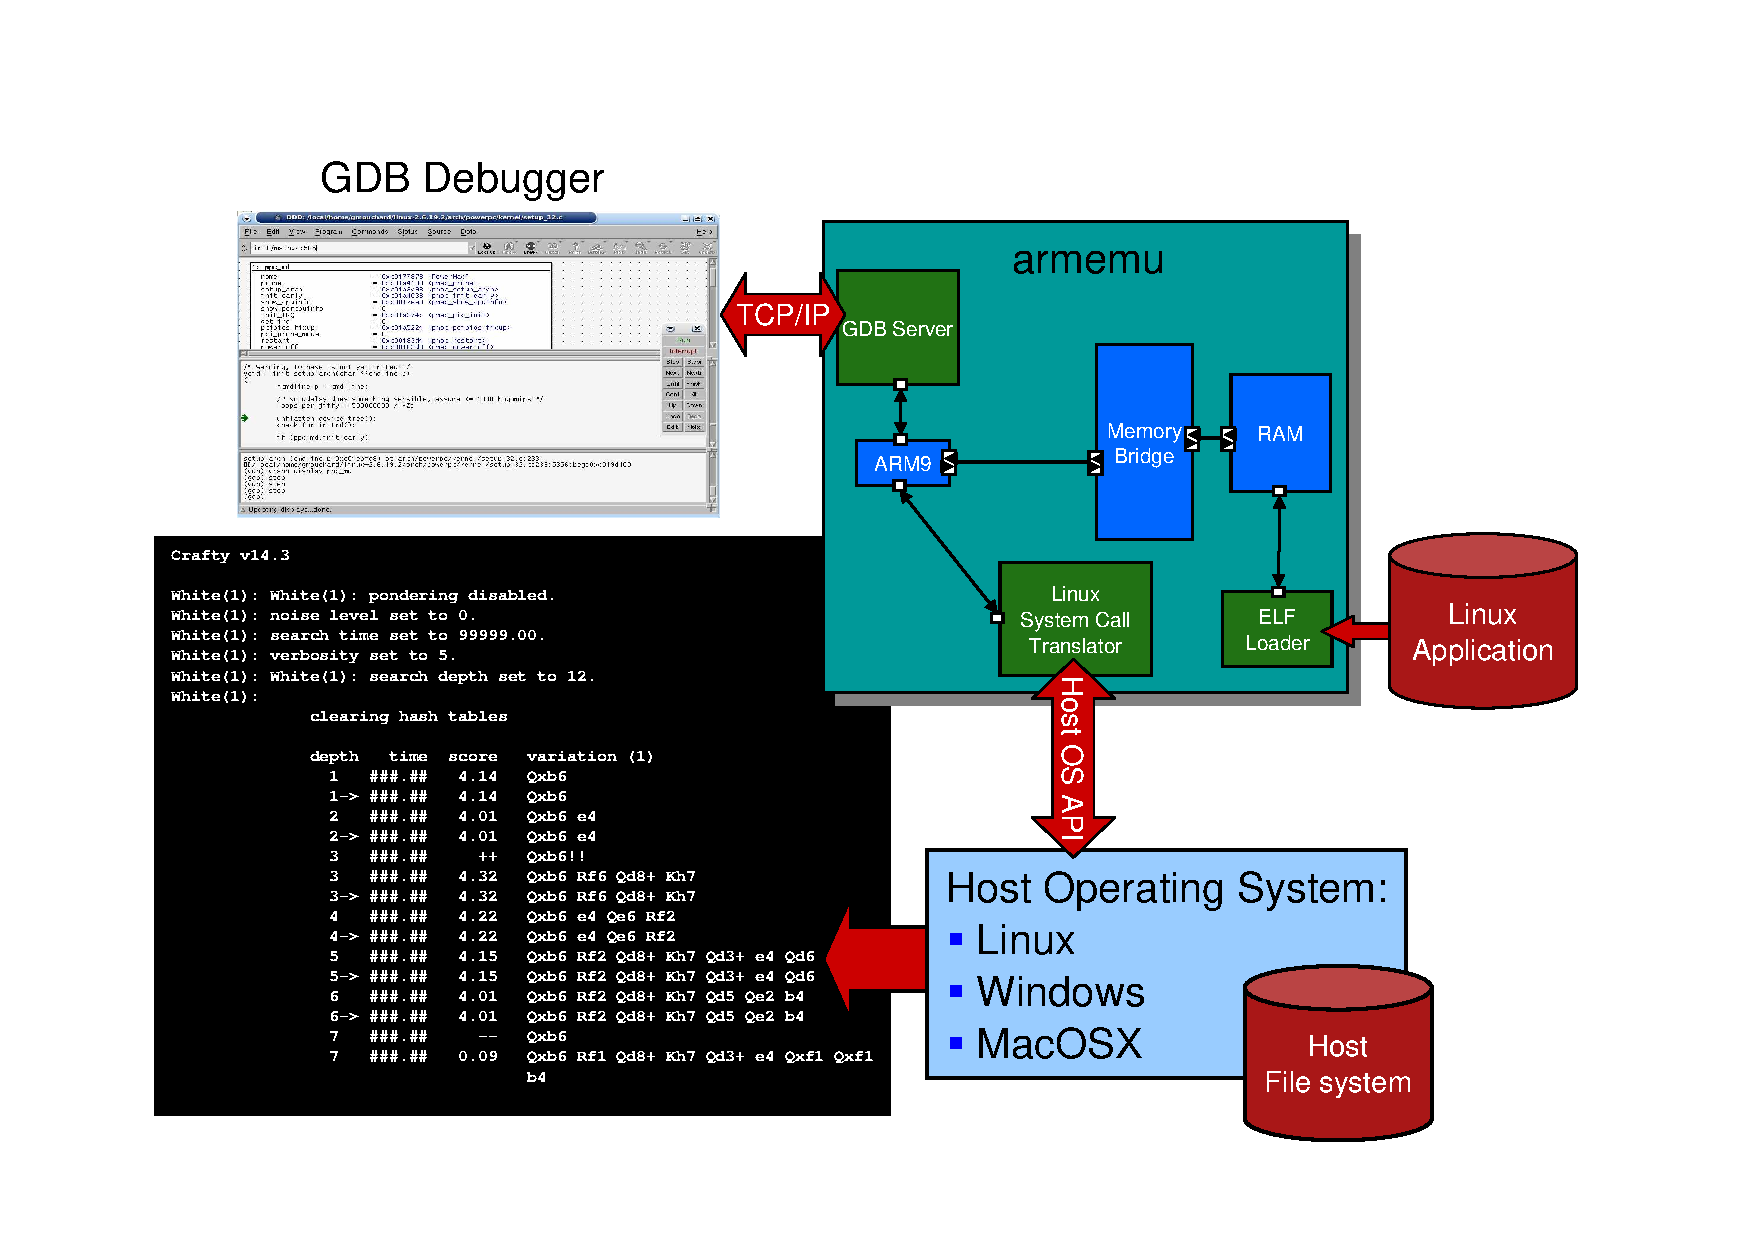
\includegraphics[width=\textwidth]{armemu/fig_schematic.pdf}
	\end{center}
	\caption{UNISIM ARMEmu simulator schematic.}
\end{figure}
\noindent The UNISIM ARMEmu simulator is composed of the following modules and services:
\begin{itemize}\addtolength{\itemsep}{-0.40\baselineskip}
\item \textbf{cpu}
\item \textbf{cpu.dcache}
\item \textbf{cpu.icache}
\item \textbf{debugger}
\item \textbf{gdb-server}: this service implements the GDB server remote serial protocol over TCP/IP. Standards GDB clients (e.g. gdb, eclipse, ddd) can connect to the simulator to debug the target application that runs within the simulator.
\item \textbf{host-time}: this service is an abstraction layer for the host machine time
\item \textbf{inline-debugger}: this service implements a built-in debugger in the terminal console
\item \textbf{linux-os}
\item \textbf{memory}: this module implements a memory
\item \textbf{profiler}
\item \textbf{tee-memory-access-reporting}
\item \textbf{tee-memory-access-reporting.tee-memory-access-reporting.control\_selector[0]}
\item \textbf{tee-memory-access-reporting.tee-memory-access-reporting.control\_selector[10]}
\item \textbf{tee-memory-access-reporting.tee-memory-access-reporting.control\_selector[11]}
\item \textbf{tee-memory-access-reporting.tee-memory-access-reporting.control\_selector[12]}
\item \textbf{tee-memory-access-reporting.tee-memory-access-reporting.control\_selector[13]}
\item \textbf{tee-memory-access-reporting.tee-memory-access-reporting.control\_selector[14]}
\item \textbf{tee-memory-access-reporting.tee-memory-access-reporting.control\_selector[15]}
\item \textbf{tee-memory-access-reporting.tee-memory-access-reporting.control\_selector[1]}
\item \textbf{tee-memory-access-reporting.tee-memory-access-reporting.control\_selector[2]}
\item \textbf{tee-memory-access-reporting.tee-memory-access-reporting.control\_selector[3]}
\item \textbf{tee-memory-access-reporting.tee-memory-access-reporting.control\_selector[4]}
\item \textbf{tee-memory-access-reporting.tee-memory-access-reporting.control\_selector[5]}
\item \textbf{tee-memory-access-reporting.tee-memory-access-reporting.control\_selector[6]}
\item \textbf{tee-memory-access-reporting.tee-memory-access-reporting.control\_selector[7]}
\item \textbf{tee-memory-access-reporting.tee-memory-access-reporting.control\_selector[8]}
\item \textbf{tee-memory-access-reporting.tee-memory-access-reporting.control\_selector[9]}
\item \textbf{time}: this service is an abstraction layer for the SystemC kernel time
\end{itemize}
\subsection{Using the UNISIM ARMEmu simulator}
\label{UNISIM ARMEmu_using}
The UNISIM ARMEmu simulator has the following command line options:\\
~\\
\noindent Usage: \texttt{unisim-armemu-0.7.1 [<options>] [...]}

\noindent Options:
\begin{itemize}
\item \texttt{--set $<$param=value$>$ or -s $<$param=value$>$}: set value of parameter 'param' to 'value'
\item \texttt{--config $<$XML file$>$ or -c $<$XML file$>$}: configures the simulator with the given XML configuration file
\item \texttt{--get-config $<$XML file$>$ or -g $<$XML file$>$}: get the simulator configuration XML file (you can use it to create your own configuration. This option can be combined with -c to get a new configuration file with existing variables from another file
\item \texttt{--list or -l}: lists all available parameters, their type, and their current value
\item \texttt{--warn or -w}: enable printing of kernel warnings
\item \texttt{--doc $<$Latex file$>$ or -d $<$Latex file$>$}: enable printing a latex documentation
\item \texttt{--version or -v}: displays the program version information
\item \texttt{--share-path $<$path$>$ or -p $<$path$>$}: the path that should be used for the share directory (absolute path)
\item \texttt{--help or -h}: displays this help
\end{itemize}
\subsection{Configuration}
\label{UNISIM ARMEmu_configuration}
Simulator configuration (see below) can be modified using command line Options \texttt{--set $<$param=value$>$} or \texttt{--config $<$config file$>$}.\\
~\\
\tablehead{\hline}
\tabletail{\hline}
\begin{supertabular}{|p{7.5cm}|p{7.5cm}|}
\multicolumn{2}{|l|}{\textbf{\Large Global}}\\
\hline
\multicolumn{1}{|p{7.5cm}}{\textbf{Name:} \texttt{enable-gdb-server}} & \multicolumn{1}{p{7.5cm}|}{\textbf{Type:} \texttt{parameter}}\\
\multicolumn{1}{|p{7.5cm}}{\textbf{Default:} \texttt{true}} & \multicolumn{1}{p{7.5cm}|}{\textbf{Data type:} \texttt{boolean}}\\
\multicolumn{2}{|p{15cm}|}{\textbf{Valid:} \texttt{true},~\texttt{false}}\\
\multicolumn{2}{|l|}{}\\
\multicolumn{2}{|p{15cm}|}{\textbf{Description:} \newline Enable GDB server..}\\
\hline
\multicolumn{1}{|p{7.5cm}}{\textbf{Name:} \texttt{enable-inline-debugger}} & \multicolumn{1}{p{7.5cm}|}{\textbf{Type:} \texttt{parameter}}\\
\multicolumn{1}{|p{7.5cm}}{\textbf{Default:} \texttt{true}} & \multicolumn{1}{p{7.5cm}|}{\textbf{Data type:} \texttt{boolean}}\\
\multicolumn{2}{|p{15cm}|}{\textbf{Valid:} \texttt{true},~\texttt{false}}\\
\multicolumn{2}{|l|}{}\\
\multicolumn{2}{|p{15cm}|}{\textbf{Description:} \newline Enable inline debugger..}\\
\hline
\multicolumn{1}{|p{7.5cm}}{\textbf{Name:} \texttt{enable-power-estimation}} & \multicolumn{1}{p{7.5cm}|}{\textbf{Type:} \texttt{parameter}}\\
\multicolumn{1}{|p{7.5cm}}{\textbf{Default:} \texttt{false}} & \multicolumn{1}{p{7.5cm}|}{\textbf{Data type:} \texttt{boolean}}\\
\multicolumn{2}{|p{15cm}|}{\textbf{Valid:} \texttt{true},~\texttt{false}}\\
\multicolumn{2}{|l|}{}\\
\multicolumn{2}{|p{15cm}|}{\textbf{Description:} \newline Activate caches power estimation..}\\
\hline
\multicolumn{1}{|p{7.5cm}}{\textbf{Name:} \texttt{enable-press-enter-at-exit}} & \multicolumn{1}{p{7.5cm}|}{\textbf{Type:} \texttt{parameter}}\\
\multicolumn{1}{|p{7.5cm}}{\textbf{Default:} \texttt{false}} & \multicolumn{1}{p{7.5cm}|}{\textbf{Data type:} \texttt{boolean}}\\
\multicolumn{2}{|p{15cm}|}{\textbf{Valid:} \texttt{true},~\texttt{false}}\\
\multicolumn{2}{|l|}{}\\
\multicolumn{2}{|p{15cm}|}{\textbf{Description:} \newline Enable/Disable pressing key enter at exit.}\\
\hline
\multicolumn{1}{|p{7.5cm}}{\textbf{Name:} \texttt{kernel\_logger.file}} & \multicolumn{1}{p{7.5cm}|}{\textbf{Type:} \texttt{parameter}}\\
\multicolumn{1}{|p{7.5cm}}{\textbf{Default:} \texttt{false}} & \multicolumn{1}{p{7.5cm}|}{\textbf{Data type:} \texttt{boolean}}\\
\multicolumn{2}{|p{15cm}|}{\textbf{Valid:} \texttt{true},~\texttt{false}}\\
\multicolumn{2}{|l|}{}\\
\multicolumn{2}{|p{15cm}|}{\textbf{Description:} \newline Keep logger output in a file.}\\
\hline
\multicolumn{1}{|p{7.5cm}}{\textbf{Name:} \texttt{kernel\_logger.filename}} & \multicolumn{1}{p{7.5cm}|}{\textbf{Type:} \texttt{parameter}}\\
\multicolumn{1}{|p{7.5cm}}{\textbf{Default:} \texttt{logger\_output.txt}} & \multicolumn{1}{p{7.5cm}|}{\textbf{Data type:} \texttt{string}}\\
\multicolumn{2}{|l|}{}\\
\multicolumn{2}{|l|}{}\\
\multicolumn{2}{|p{15cm}|}{\textbf{Description:} \newline Filename to keep logger output \_(the option file must be activated).}\\
\hline
\multicolumn{1}{|p{7.5cm}}{\textbf{Name:} \texttt{kernel\_logger.std\_err}} & \multicolumn{1}{p{7.5cm}|}{\textbf{Type:} \texttt{parameter}}\\
\multicolumn{1}{|p{7.5cm}}{\textbf{Default:} \texttt{true}} & \multicolumn{1}{p{7.5cm}|}{\textbf{Data type:} \texttt{boolean}}\\
\multicolumn{2}{|p{15cm}|}{\textbf{Valid:} \texttt{true},~\texttt{false}}\\
\multicolumn{2}{|l|}{}\\
\multicolumn{2}{|p{15cm}|}{\textbf{Description:} \newline Show logger output through the standard error output.}\\
\hline
\multicolumn{1}{|p{7.5cm}}{\textbf{Name:} \texttt{kernel\_logger.std\_err\_color}} & \multicolumn{1}{p{7.5cm}|}{\textbf{Type:} \texttt{parameter}}\\
\multicolumn{1}{|p{7.5cm}}{\textbf{Default:} \texttt{true}} & \multicolumn{1}{p{7.5cm}|}{\textbf{Data type:} \texttt{boolean}}\\
\multicolumn{2}{|p{15cm}|}{\textbf{Valid:} \texttt{true},~\texttt{false}}\\
\multicolumn{2}{|l|}{}\\
\multicolumn{2}{|p{15cm}|}{\textbf{Description:} \newline Colorize logger output through the standard error output \_(only works if std\_err is active).}\\
\hline
\multicolumn{1}{|p{7.5cm}}{\textbf{Name:} \texttt{kernel\_logger.std\_out}} & \multicolumn{1}{p{7.5cm}|}{\textbf{Type:} \texttt{parameter}}\\
\multicolumn{1}{|p{7.5cm}}{\textbf{Default:} \texttt{false}} & \multicolumn{1}{p{7.5cm}|}{\textbf{Data type:} \texttt{boolean}}\\
\multicolumn{2}{|p{15cm}|}{\textbf{Valid:} \texttt{true},~\texttt{false}}\\
\multicolumn{2}{|l|}{}\\
\multicolumn{2}{|p{15cm}|}{\textbf{Description:} \newline Show logger output through the standard output.}\\
\hline
\multicolumn{1}{|p{7.5cm}}{\textbf{Name:} \texttt{kernel\_logger.std\_out\_color}} & \multicolumn{1}{p{7.5cm}|}{\textbf{Type:} \texttt{parameter}}\\
\multicolumn{1}{|p{7.5cm}}{\textbf{Default:} \texttt{false}} & \multicolumn{1}{p{7.5cm}|}{\textbf{Data type:} \texttt{boolean}}\\
\multicolumn{2}{|p{15cm}|}{\textbf{Valid:} \texttt{true},~\texttt{false}}\\
\multicolumn{2}{|l|}{}\\
\multicolumn{2}{|p{15cm}|}{\textbf{Description:} \newline Colorize logger output through the standard output \_(only works if std\_out is active).}\\
\hline
\multicolumn{1}{|p{7.5cm}}{\textbf{Name:} \texttt{kernel\_logger.xml\_file}} & \multicolumn{1}{p{7.5cm}|}{\textbf{Type:} \texttt{parameter}}\\
\multicolumn{1}{|p{7.5cm}}{\textbf{Default:} \texttt{false}} & \multicolumn{1}{p{7.5cm}|}{\textbf{Data type:} \texttt{boolean}}\\
\multicolumn{2}{|p{15cm}|}{\textbf{Valid:} \texttt{true},~\texttt{false}}\\
\multicolumn{2}{|l|}{}\\
\multicolumn{2}{|p{15cm}|}{\textbf{Description:} \newline Keep logger output in a file xml formatted.}\\
\hline
\multicolumn{1}{|p{7.5cm}}{\textbf{Name:} \texttt{kernel\_logger.xml\_file\_gzipped}} & \multicolumn{1}{p{7.5cm}|}{\textbf{Type:} \texttt{parameter}}\\
\multicolumn{1}{|p{7.5cm}}{\textbf{Default:} \texttt{false}} & \multicolumn{1}{p{7.5cm}|}{\textbf{Data type:} \texttt{boolean}}\\
\multicolumn{2}{|p{15cm}|}{\textbf{Valid:} \texttt{true},~\texttt{false}}\\
\multicolumn{2}{|l|}{}\\
\multicolumn{2}{|p{15cm}|}{\textbf{Description:} \newline If the xml\_file option is active, the output file will be compressed (a .gz extension will be automatically added to the xml\_filename option.}\\
\hline
\multicolumn{1}{|p{7.5cm}}{\textbf{Name:} \texttt{kernel\_logger.xml\_filename}} & \multicolumn{1}{p{7.5cm}|}{\textbf{Type:} \texttt{parameter}}\\
\multicolumn{1}{|p{7.5cm}}{\textbf{Default:} \texttt{logger\_output.xml}} & \multicolumn{1}{p{7.5cm}|}{\textbf{Data type:} \texttt{string}}\\
\multicolumn{2}{|l|}{}\\
\multicolumn{2}{|l|}{}\\
\multicolumn{2}{|p{15cm}|}{\textbf{Description:} \newline Filename to keep logger xml output \_(the option xml\_file must be activated).}\\
\hline
\hline
\multicolumn{2}{|l|}{\textbf{\Large cpu}}\\
\hline
\multicolumn{1}{|p{7.5cm}}{\textbf{Name:} \texttt{cpu.default-endianness}} & \multicolumn{1}{p{7.5cm}|}{\textbf{Type:} \texttt{parameter}}\\
\multicolumn{1}{|p{7.5cm}}{\textbf{Default:} \texttt{little-endian}} & \multicolumn{1}{p{7.5cm}|}{\textbf{Data type:} \texttt{string}}\\
\multicolumn{2}{|l|}{}\\
\multicolumn{2}{|l|}{}\\
\multicolumn{2}{|p{15cm}|}{\textbf{Description:} \newline The processor default/boot endianness. Available values are: little-endian and big-endian..}\\
\hline
\multicolumn{1}{|p{7.5cm}}{\textbf{Name:} \texttt{cpu.voltage}} & \multicolumn{1}{p{7.5cm}|}{\textbf{Type:} \texttt{parameter}}\\
\multicolumn{1}{|p{7.5cm}}{\textbf{Default:} \texttt{1800}} & \multicolumn{1}{p{7.5cm}|}{\textbf{Data type:} \texttt{unsigned 64-bit integer}}\\
\multicolumn{2}{|l|}{}\\
\multicolumn{2}{|l|}{}\\
\multicolumn{2}{|p{15cm}|}{\textbf{Description:} \newline The processor voltage in mV..}\\
\hline
\multicolumn{1}{|p{7.5cm}}{\textbf{Name:} \texttt{cpu.verbose}} & \multicolumn{1}{p{7.5cm}|}{\textbf{Type:} \texttt{parameter}}\\
\multicolumn{1}{|p{7.5cm}}{\textbf{Default:} \texttt{0x00000000}} & \multicolumn{1}{p{7.5cm}|}{\textbf{Data type:} \texttt{unsigned 32-bit integer}}\\
\multicolumn{2}{|l|}{}\\
\multicolumn{2}{|l|}{}\\
\multicolumn{2}{|p{15cm}|}{\textbf{Description:} \newline Activate the verbose system (0 = inactive, different than 0 = active)..}\\
\hline
\multicolumn{1}{|p{7.5cm}}{\textbf{Name:} \texttt{cpu.trap-on-instruction-counter}} & \multicolumn{1}{p{7.5cm}|}{\textbf{Type:} \texttt{parameter}}\\
\multicolumn{1}{|p{7.5cm}}{\textbf{Default:} \texttt{0}} & \multicolumn{1}{p{7.5cm}|}{\textbf{Data type:} \texttt{unsigned 64-bit integer}}\\
\multicolumn{2}{|l|}{}\\
\multicolumn{2}{|l|}{}\\
\multicolumn{2}{|p{15cm}|}{\textbf{Description:} \newline Produce a trap when the given instruction count is reached..}\\
\hline
\multicolumn{1}{|p{7.5cm}}{\textbf{Name:} \texttt{cpu.cpu-cycle-time}} & \multicolumn{1}{p{7.5cm}|}{\textbf{Type:} \texttt{parameter}}\\
\multicolumn{1}{|p{7.5cm}}{\textbf{Default:} \texttt{31250 ps}} & \multicolumn{1}{p{7.5cm}|}{\textbf{Data type:} \texttt{sc\_time}}\\
\multicolumn{2}{|l|}{}\\
\multicolumn{2}{|l|}{}\\
\multicolumn{2}{|p{15cm}|}{\textbf{Description:} \newline The processor cycle time..}\\
\hline
\multicolumn{1}{|p{7.5cm}}{\textbf{Name:} \texttt{cpu.bus-cycle-time}} & \multicolumn{1}{p{7.5cm}|}{\textbf{Type:} \texttt{parameter}}\\
\multicolumn{1}{|p{7.5cm}}{\textbf{Default:} \texttt{31250 ps}} & \multicolumn{1}{p{7.5cm}|}{\textbf{Data type:} \texttt{sc\_time}}\\
\multicolumn{2}{|l|}{}\\
\multicolumn{2}{|l|}{}\\
\multicolumn{2}{|p{15cm}|}{\textbf{Description:} \newline The processor bus cycle time..}\\
\hline
\multicolumn{1}{|p{7.5cm}}{\textbf{Name:} \texttt{cpu.nice-time}} & \multicolumn{1}{p{7.5cm}|}{\textbf{Type:} \texttt{parameter}}\\
\multicolumn{1}{|p{7.5cm}}{\textbf{Default:} \texttt{1 ms}} & \multicolumn{1}{p{7.5cm}|}{\textbf{Data type:} \texttt{sc\_time}}\\
\multicolumn{2}{|l|}{}\\
\multicolumn{2}{|l|}{}\\
\multicolumn{2}{|p{15cm}|}{\textbf{Description:} \newline Maximum time between SystemC waits..}\\
\hline
\multicolumn{1}{|p{7.5cm}}{\textbf{Name:} \texttt{cpu.ipc}} & \multicolumn{1}{p{7.5cm}|}{\textbf{Type:} \texttt{parameter}}\\
\multicolumn{1}{|p{7.5cm}}{\textbf{Default:} \texttt{1}} & \multicolumn{1}{p{7.5cm}|}{\textbf{Data type:} \texttt{double precision floating-point}}\\
\multicolumn{2}{|l|}{}\\
\multicolumn{2}{|l|}{}\\
\multicolumn{2}{|p{15cm}|}{\textbf{Description:} \newline Instructions per cycle performance..}\\
\hline
\multicolumn{1}{|p{7.5cm}}{\textbf{Name:} \texttt{cpu.verbose-tlm}} & \multicolumn{1}{p{7.5cm}|}{\textbf{Type:} \texttt{parameter}}\\
\multicolumn{1}{|p{7.5cm}}{\textbf{Default:} \texttt{false}} & \multicolumn{1}{p{7.5cm}|}{\textbf{Data type:} \texttt{boolean}}\\
\multicolumn{2}{|p{15cm}|}{\textbf{Valid:} \texttt{true},~\texttt{false}}\\
\multicolumn{2}{|l|}{}\\
\multicolumn{2}{|p{15cm}|}{\textbf{Description:} \newline Display TLM information.}\\
\hline
\hline
\multicolumn{2}{|l|}{\textbf{\Large cpu.dcache}}\\
\hline
\multicolumn{1}{|p{7.5cm}}{\textbf{Name:} \texttt{cpu.dcache.size}} & \multicolumn{1}{p{7.5cm}|}{\textbf{Type:} \texttt{parameter}}\\
\multicolumn{1}{|p{7.5cm}}{\textbf{Default:} \texttt{131072}} & \multicolumn{1}{p{7.5cm}|}{\textbf{Data type:} \texttt{unsigned 32-bit integer}}\\
\multicolumn{2}{|l|}{}\\
\multicolumn{2}{|l|}{}\\
\multicolumn{2}{|p{15cm}|}{\textbf{Description:} \newline Size of the cache in bytes. Avalaible sizes are 4KB, 8KB, 16KB, 32KB, 64KB and 128KB. The cache can be deactivated setting this value to 0..}\\
\hline
\hline
\multicolumn{2}{|l|}{\textbf{\Large cpu.icache}}\\
\hline
\multicolumn{1}{|p{7.5cm}}{\textbf{Name:} \texttt{cpu.icache.size}} & \multicolumn{1}{p{7.5cm}|}{\textbf{Type:} \texttt{parameter}}\\
\multicolumn{1}{|p{7.5cm}}{\textbf{Default:} \texttt{131072}} & \multicolumn{1}{p{7.5cm}|}{\textbf{Data type:} \texttt{unsigned 32-bit integer}}\\
\multicolumn{2}{|l|}{}\\
\multicolumn{2}{|l|}{}\\
\multicolumn{2}{|p{15cm}|}{\textbf{Description:} \newline Size of the cache in bytes. Avalaible sizes are 4KB, 8KB, 16KB, 32KB, 64KB and 128KB. The cache can be deactivated setting this value to 0..}\\
\hline
\hline
\multicolumn{2}{|l|}{\textbf{\Large debugger}}\\
\hline
\multicolumn{1}{|p{7.5cm}}{\textbf{Name:} \texttt{debugger.verbose}} & \multicolumn{1}{p{7.5cm}|}{\textbf{Type:} \texttt{parameter}}\\
\multicolumn{1}{|p{7.5cm}}{\textbf{Default:} \texttt{false}} & \multicolumn{1}{p{7.5cm}|}{\textbf{Data type:} \texttt{boolean}}\\
\multicolumn{2}{|p{15cm}|}{\textbf{Valid:} \texttt{true},~\texttt{false}}\\
\multicolumn{2}{|l|}{}\\
\multicolumn{2}{|p{15cm}|}{\textbf{Description:} \newline Enable/Disable verbosity.}\\
\hline
\multicolumn{1}{|p{7.5cm}}{\textbf{Name:} \texttt{debugger.dwarf-to-html-output-} \newline$\hookrightarrow$\texttt{directory}} & \multicolumn{1}{p{7.5cm}|}{\textbf{Type:} \texttt{parameter}}\\
\multicolumn{1}{|p{7.5cm}}{\textbf{Default:} \texttt{}} & \multicolumn{1}{p{7.5cm}|}{\textbf{Data type:} \texttt{string}}\\
\multicolumn{2}{|l|}{}\\
\multicolumn{2}{|l|}{}\\
\multicolumn{2}{|p{15cm}|}{\textbf{Description:} \newline DWARF v2/v3 to HTML output directory.}\\
\hline
\multicolumn{1}{|p{7.5cm}}{\textbf{Name:} \texttt{debugger.dwarf-register-number-} \newline$\hookrightarrow$\texttt{mapping-filename}} & \multicolumn{1}{p{7.5cm}|}{\textbf{Type:} \texttt{parameter}}\\
\multicolumn{1}{|p{7.5cm}}{\textbf{Default:} \texttt{arm\_eabi\_dwarf\_register\_} \newline$\hookrightarrow$\texttt{number\_mapping.xml}} & \multicolumn{1}{p{7.5cm}|}{\textbf{Data type:} \texttt{string}}\\
\multicolumn{2}{|l|}{}\\
\multicolumn{2}{|l|}{}\\
\multicolumn{2}{|p{15cm}|}{\textbf{Description:} \newline DWARF register number mapping filename.}\\
\hline
\multicolumn{1}{|p{7.5cm}}{\textbf{Name:} \texttt{debugger.parse-dwarf}} & \multicolumn{1}{p{7.5cm}|}{\textbf{Type:} \texttt{parameter}}\\
\multicolumn{1}{|p{7.5cm}}{\textbf{Default:} \texttt{true}} & \multicolumn{1}{p{7.5cm}|}{\textbf{Data type:} \texttt{boolean}}\\
\multicolumn{2}{|p{15cm}|}{\textbf{Valid:} \texttt{true},~\texttt{false}}\\
\multicolumn{2}{|l|}{}\\
\multicolumn{2}{|p{15cm}|}{\textbf{Description:} \newline Enable/Disable parsing of DWARF debugging informations.}\\
\hline
\multicolumn{1}{|p{7.5cm}}{\textbf{Name:} \texttt{debugger.debug-dwarf}} & \multicolumn{1}{p{7.5cm}|}{\textbf{Type:} \texttt{parameter}}\\
\multicolumn{1}{|p{7.5cm}}{\textbf{Default:} \texttt{false}} & \multicolumn{1}{p{7.5cm}|}{\textbf{Data type:} \texttt{boolean}}\\
\multicolumn{2}{|p{15cm}|}{\textbf{Valid:} \texttt{true},~\texttt{false}}\\
\multicolumn{2}{|l|}{}\\
\multicolumn{2}{|p{15cm}|}{\textbf{Description:} \newline Enable/Disable debugging of DWARF.}\\
\hline
\hline
\multicolumn{2}{|l|}{\textbf{\Large gdb-server}}\\
\hline
\multicolumn{1}{|p{7.5cm}}{\textbf{Name:} \texttt{gdb-server.memory-atom-size}} & \multicolumn{1}{p{7.5cm}|}{\textbf{Type:} \texttt{parameter}}\\
\multicolumn{1}{|p{7.5cm}}{\textbf{Default:} \texttt{0x00000001}} & \multicolumn{1}{p{7.5cm}|}{\textbf{Data type:} \texttt{unsigned 32-bit integer}}\\
\multicolumn{2}{|l|}{}\\
\multicolumn{2}{|l|}{}\\
\multicolumn{2}{|p{15cm}|}{\textbf{Description:} \newline size of the smallest addressable element in memory.}\\
\hline
\multicolumn{1}{|p{7.5cm}}{\textbf{Name:} \texttt{gdb-server.tcp-port}} & \multicolumn{1}{p{7.5cm}|}{\textbf{Type:} \texttt{parameter}}\\
\multicolumn{1}{|p{7.5cm}}{\textbf{Default:} \texttt{12345}} & \multicolumn{1}{p{7.5cm}|}{\textbf{Data type:} \texttt{signed 32-bit integer}}\\
\multicolumn{2}{|l|}{}\\
\multicolumn{2}{|l|}{}\\
\multicolumn{2}{|p{15cm}|}{\textbf{Description:} \newline TCP/IP port to listen waiting for a GDB client connection.}\\
\hline
\multicolumn{1}{|p{7.5cm}}{\textbf{Name:} \texttt{gdb-server.architecture-description-} \newline$\hookrightarrow$\texttt{filename}} & \multicolumn{1}{p{7.5cm}|}{\textbf{Type:} \texttt{parameter}}\\
\multicolumn{1}{|p{7.5cm}}{\textbf{Default:} \texttt{gdb\_armv5l.xml}} & \multicolumn{1}{p{7.5cm}|}{\textbf{Data type:} \texttt{string}}\\
\multicolumn{2}{|l|}{}\\
\multicolumn{2}{|l|}{}\\
\multicolumn{2}{|p{15cm}|}{\textbf{Description:} \newline filename of a XML description of the connected processor.}\\
\hline
\multicolumn{1}{|p{7.5cm}}{\textbf{Name:} \texttt{gdb-server.verbose}} & \multicolumn{1}{p{7.5cm}|}{\textbf{Type:} \texttt{parameter}}\\
\multicolumn{1}{|p{7.5cm}}{\textbf{Default:} \texttt{false}} & \multicolumn{1}{p{7.5cm}|}{\textbf{Data type:} \texttt{boolean}}\\
\multicolumn{2}{|p{15cm}|}{\textbf{Valid:} \texttt{true},~\texttt{false}}\\
\multicolumn{2}{|l|}{}\\
\multicolumn{2}{|p{15cm}|}{\textbf{Description:} \newline Enable/Disable verbosity.}\\
\hline
\hline
\multicolumn{2}{|l|}{\textbf{\Large inline-debugger}}\\
\hline
\multicolumn{1}{|p{7.5cm}}{\textbf{Name:} \texttt{inline-debugger.memory-atom-} \newline$\hookrightarrow$\texttt{size}} & \multicolumn{1}{p{7.5cm}|}{\textbf{Type:} \texttt{parameter}}\\
\multicolumn{1}{|p{7.5cm}}{\textbf{Default:} \texttt{0x00000001}} & \multicolumn{1}{p{7.5cm}|}{\textbf{Data type:} \texttt{unsigned 32-bit integer}}\\
\multicolumn{2}{|l|}{}\\
\multicolumn{2}{|l|}{}\\
\multicolumn{2}{|p{15cm}|}{\textbf{Description:} \newline size of the smallest addressable element in memory.}\\
\hline
\multicolumn{1}{|p{7.5cm}}{\textbf{Name:} \texttt{inline-debugger.search-path}} & \multicolumn{1}{p{7.5cm}|}{\textbf{Type:} \texttt{parameter}}\\
\multicolumn{1}{|p{7.5cm}}{\textbf{Default:} \texttt{}} & \multicolumn{1}{p{7.5cm}|}{\textbf{Data type:} \texttt{string}}\\
\multicolumn{2}{|l|}{}\\
\multicolumn{2}{|l|}{}\\
\multicolumn{2}{|p{15cm}|}{\textbf{Description:} \newline Search path for source (separated by ';').}\\
\hline
\multicolumn{1}{|p{7.5cm}}{\textbf{Name:} \texttt{inline-debugger.init-macro}} & \multicolumn{1}{p{7.5cm}|}{\textbf{Type:} \texttt{parameter}}\\
\multicolumn{1}{|p{7.5cm}}{\textbf{Default:} \texttt{}} & \multicolumn{1}{p{7.5cm}|}{\textbf{Data type:} \texttt{string}}\\
\multicolumn{2}{|l|}{}\\
\multicolumn{2}{|l|}{}\\
\multicolumn{2}{|p{15cm}|}{\textbf{Description:} \newline path to initial macro to run when debugger starts.}\\
\hline
\multicolumn{1}{|p{7.5cm}}{\textbf{Name:} \texttt{inline-debugger.output}} & \multicolumn{1}{p{7.5cm}|}{\textbf{Type:} \texttt{parameter}}\\
\multicolumn{1}{|p{7.5cm}}{\textbf{Default:} \texttt{}} & \multicolumn{1}{p{7.5cm}|}{\textbf{Data type:} \texttt{string}}\\
\multicolumn{2}{|l|}{}\\
\multicolumn{2}{|l|}{}\\
\multicolumn{2}{|p{15cm}|}{\textbf{Description:} \newline path to output file where to redirect the debugger outputs.}\\
\hline
\hline
\multicolumn{2}{|l|}{\textbf{\Large linux-os}}\\
\hline
\multicolumn{1}{|p{7.5cm}}{\textbf{Name:} \texttt{linux-os.verbose}} & \multicolumn{1}{p{7.5cm}|}{\textbf{Type:} \texttt{parameter}}\\
\multicolumn{1}{|p{7.5cm}}{\textbf{Default:} \texttt{false}} & \multicolumn{1}{p{7.5cm}|}{\textbf{Data type:} \texttt{boolean}}\\
\multicolumn{2}{|p{15cm}|}{\textbf{Valid:} \texttt{true},~\texttt{false}}\\
\hline
\multicolumn{1}{|p{7.5cm}}{\textbf{Name:} \texttt{linux-os.parse-dwarf}} & \multicolumn{1}{p{7.5cm}|}{\textbf{Type:} \texttt{parameter}}\\
\multicolumn{1}{|p{7.5cm}}{\textbf{Default:} \texttt{false}} & \multicolumn{1}{p{7.5cm}|}{\textbf{Data type:} \texttt{boolean}}\\
\multicolumn{2}{|p{15cm}|}{\textbf{Valid:} \texttt{true},~\texttt{false}}\\
\hline
\multicolumn{1}{|p{7.5cm}}{\textbf{Name:} \texttt{linux-os.debug-dwarf}} & \multicolumn{1}{p{7.5cm}|}{\textbf{Type:} \texttt{parameter}}\\
\multicolumn{1}{|p{7.5cm}}{\textbf{Default:} \texttt{false}} & \multicolumn{1}{p{7.5cm}|}{\textbf{Data type:} \texttt{boolean}}\\
\multicolumn{2}{|p{15cm}|}{\textbf{Valid:} \texttt{true},~\texttt{false}}\\
\hline
\multicolumn{1}{|p{7.5cm}}{\textbf{Name:} \texttt{linux-os.dwarf-to-html-output-} \newline$\hookrightarrow$\texttt{directory}} & \multicolumn{1}{p{7.5cm}|}{\textbf{Type:} \texttt{parameter}}\\
\multicolumn{1}{|p{7.5cm}}{\textbf{Default:} \texttt{}} & \multicolumn{1}{p{7.5cm}|}{\textbf{Data type:} \texttt{string}}\\
\multicolumn{2}{|l|}{}\\
\hline
\multicolumn{1}{|p{7.5cm}}{\textbf{Name:} \texttt{linux-os.dwarf-to-xml-output-} \newline$\hookrightarrow$\texttt{filename}} & \multicolumn{1}{p{7.5cm}|}{\textbf{Type:} \texttt{parameter}}\\
\multicolumn{1}{|p{7.5cm}}{\textbf{Default:} \texttt{}} & \multicolumn{1}{p{7.5cm}|}{\textbf{Data type:} \texttt{string}}\\
\multicolumn{2}{|l|}{}\\
\hline
\multicolumn{1}{|p{7.5cm}}{\textbf{Name:} \texttt{linux-os.system}} & \multicolumn{1}{p{7.5cm}|}{\textbf{Type:} \texttt{parameter}}\\
\multicolumn{1}{|p{7.5cm}}{\textbf{Default:} \texttt{arm-eabi}} & \multicolumn{1}{p{7.5cm}|}{\textbf{Data type:} \texttt{string}}\\
\multicolumn{2}{|l|}{}\\
\multicolumn{2}{|l|}{}\\
\multicolumn{2}{|p{15cm}|}{\textbf{Description:} \newline Emulated system architecture available values are "arm", "arm-eabi" and "powerpc".}\\
\hline
\multicolumn{1}{|p{7.5cm}}{\textbf{Name:} \texttt{linux-os.endianness}} & \multicolumn{1}{p{7.5cm}|}{\textbf{Type:} \texttt{parameter}}\\
\multicolumn{1}{|p{7.5cm}}{\textbf{Default:} \texttt{little-endian}} & \multicolumn{1}{p{7.5cm}|}{\textbf{Data type:} \texttt{endianess}}\\
\multicolumn{2}{|p{15cm}|}{\textbf{Valid:} \texttt{little-endian},~\texttt{big-endian}}\\
\multicolumn{2}{|l|}{}\\
\multicolumn{2}{|p{15cm}|}{\textbf{Description:} \newline The endianness of the binary loaded. Available values are: little-endian and big-endian..}\\
\hline
\multicolumn{1}{|p{7.5cm}}{\textbf{Name:} \texttt{linux-os.memory-page-size}} & \multicolumn{1}{p{7.5cm}|}{\textbf{Type:} \texttt{parameter}}\\
\multicolumn{1}{|p{7.5cm}}{\textbf{Default:} \texttt{0x00001000}} & \multicolumn{1}{p{7.5cm}|}{\textbf{Data type:} \texttt{unsigned 32-bit integer}}\\
\multicolumn{2}{|l|}{}\\
\hline
\multicolumn{1}{|p{7.5cm}}{\textbf{Name:} \texttt{linux-os.stack-base}} & \multicolumn{1}{p{7.5cm}|}{\textbf{Type:} \texttt{parameter}}\\
\multicolumn{1}{|p{7.5cm}}{\textbf{Default:} \texttt{0x40000000}} & \multicolumn{1}{p{7.5cm}|}{\textbf{Data type:} \texttt{unsigned 32-bit integer}}\\
\multicolumn{2}{|l|}{}\\
\multicolumn{2}{|l|}{}\\
\multicolumn{2}{|p{15cm}|}{\textbf{Description:} \newline The stack base address used for the load and execution of the linux application.}\\
\hline
\multicolumn{1}{|p{7.5cm}}{\textbf{Name:} \texttt{linux-os.binary}} & \multicolumn{1}{p{7.5cm}|}{\textbf{Type:} \texttt{parameter}}\\
\multicolumn{1}{|p{7.5cm}}{\textbf{Default:} \texttt{}} & \multicolumn{1}{p{7.5cm}|}{\textbf{Data type:} \texttt{string}}\\
\multicolumn{2}{|l|}{}\\
\multicolumn{2}{|l|}{}\\
\multicolumn{2}{|p{15cm}|}{\textbf{Description:} \newline The binary to execute on the target simulator. Usually it is the same value than the argv[1] parameter..}\\
\hline
\multicolumn{1}{|p{7.5cm}}{\textbf{Name:} \texttt{linux-os.argc}} & \multicolumn{1}{p{7.5cm}|}{\textbf{Type:} \texttt{parameter}}\\
\multicolumn{1}{|p{7.5cm}}{\textbf{Default:} \texttt{0}} & \multicolumn{1}{p{7.5cm}|}{\textbf{Data type:} \texttt{unsigned 32-bit integer}}\\
\multicolumn{2}{|l|}{}\\
\multicolumn{2}{|l|}{}\\
\multicolumn{2}{|p{15cm}|}{\textbf{Description:} \newline Number of commands in the program execution line (usually at least one which is the name of the program executed). The different tokens can be set up with the parameters argv[$<$n$>$] where $<$n$>$ can go up to argc - 1..}\\
\hline
\multicolumn{1}{|p{7.5cm}}{\textbf{Name:} \texttt{linux-os.apply-host-environment}} & \multicolumn{1}{p{7.5cm}|}{\textbf{Type:} \texttt{parameter}}\\
\multicolumn{1}{|p{7.5cm}}{\textbf{Default:} \texttt{false}} & \multicolumn{1}{p{7.5cm}|}{\textbf{Data type:} \texttt{boolean}}\\
\multicolumn{2}{|p{15cm}|}{\textbf{Valid:} \texttt{true},~\texttt{false}}\\
\multicolumn{2}{|l|}{}\\
\multicolumn{2}{|p{15cm}|}{\textbf{Description:} \newline Wether to apply the host environment on the target simulator or use the provided envc and envp..}\\
\hline
\multicolumn{1}{|p{7.5cm}}{\textbf{Name:} \texttt{linux-os.envc}} & \multicolumn{1}{p{7.5cm}|}{\textbf{Type:} \texttt{parameter}}\\
\multicolumn{1}{|p{7.5cm}}{\textbf{Default:} \texttt{0x00000000}} & \multicolumn{1}{p{7.5cm}|}{\textbf{Data type:} \texttt{unsigned 32-bit integer}}\\
\multicolumn{2}{|l|}{}\\
\multicolumn{2}{|l|}{}\\
\multicolumn{2}{|p{15cm}|}{\textbf{Description:} \newline Number of environment variables defined for the program execution. The different variables can be set up with the parameters envp[$<$n$>$] where $<$n$>$ can go up to envc - 1..}\\
\hline
\multicolumn{1}{|p{7.5cm}}{\textbf{Name:} \texttt{linux-os.utsname-sysname}} & \multicolumn{1}{p{7.5cm}|}{\textbf{Type:} \texttt{parameter}}\\
\multicolumn{1}{|p{7.5cm}}{\textbf{Default:} \texttt{Linux}} & \multicolumn{1}{p{7.5cm}|}{\textbf{Data type:} \texttt{string}}\\
\multicolumn{2}{|l|}{}\\
\multicolumn{2}{|l|}{}\\
\multicolumn{2}{|p{15cm}|}{\textbf{Description:} \newline The value that the uname system call should return. As this service is providing linux emulation supoort its value should be 'Linux', so you should not modify it..}\\
\hline
\multicolumn{1}{|p{7.5cm}}{\textbf{Name:} \texttt{linux-os.utsname-nodename}} & \multicolumn{1}{p{7.5cm}|}{\textbf{Type:} \texttt{parameter}}\\
\multicolumn{1}{|p{7.5cm}}{\textbf{Default:} \texttt{localhost}} & \multicolumn{1}{p{7.5cm}|}{\textbf{Data type:} \texttt{string}}\\
\multicolumn{2}{|l|}{}\\
\multicolumn{2}{|l|}{}\\
\multicolumn{2}{|p{15cm}|}{\textbf{Description:} \newline The network node hostname that the uname system call should return. Default value is localhost, but you could write whatever name you want..}\\
\hline
\multicolumn{1}{|p{7.5cm}}{\textbf{Name:} \texttt{linux-os.utsname-release}} & \multicolumn{1}{p{7.5cm}|}{\textbf{Type:} \texttt{parameter}}\\
\multicolumn{1}{|p{7.5cm}}{\textbf{Default:} \texttt{2.6.27.35}} & \multicolumn{1}{p{7.5cm}|}{\textbf{Data type:} \texttt{string}}\\
\multicolumn{2}{|l|}{}\\
\multicolumn{2}{|l|}{}\\
\multicolumn{2}{|p{15cm}|}{\textbf{Description:} \newline The kernel realese information that the uname system call should return. This should usually match the linux-kernel parameter..}\\
\hline
\multicolumn{1}{|p{7.5cm}}{\textbf{Name:} \texttt{linux-os.utsname-version}} & \multicolumn{1}{p{7.5cm}|}{\textbf{Type:} \texttt{parameter}}\\
\multicolumn{1}{|p{7.5cm}}{\textbf{Default:} \texttt{\#UNISIM SMP Fri Mar 12 05:23:09 } \newline$\hookrightarrow$\texttt{UTC 2010}} & \multicolumn{1}{p{7.5cm}|}{\textbf{Data type:} \texttt{string}}\\
\multicolumn{2}{|l|}{}\\
\multicolumn{2}{|l|}{}\\
\multicolumn{2}{|p{15cm}|}{\textbf{Description:} \newline The kernel version information that the uname system call should return..}\\
\hline
\multicolumn{1}{|p{7.5cm}}{\textbf{Name:} \texttt{linux-os.utsname-machine}} & \multicolumn{1}{p{7.5cm}|}{\textbf{Type:} \texttt{parameter}}\\
\multicolumn{1}{|p{7.5cm}}{\textbf{Default:} \texttt{armv5}} & \multicolumn{1}{p{7.5cm}|}{\textbf{Data type:} \texttt{string}}\\
\multicolumn{2}{|l|}{}\\
\multicolumn{2}{|l|}{}\\
\multicolumn{2}{|p{15cm}|}{\textbf{Description:} \newline The machine information that the uname system call should  return. This should be one of the supported architectures (the  system parameter, that is, arm or powerpc) or a specific model  derived from it (i.e., arm926ejs)..}\\
\hline
\multicolumn{1}{|p{7.5cm}}{\textbf{Name:} \texttt{linux-os.utsname-domainname}} & \multicolumn{1}{p{7.5cm}|}{\textbf{Type:} \texttt{parameter}}\\
\multicolumn{1}{|p{7.5cm}}{\textbf{Default:} \texttt{localhost}} & \multicolumn{1}{p{7.5cm}|}{\textbf{Data type:} \texttt{string}}\\
\multicolumn{2}{|l|}{}\\
\multicolumn{2}{|l|}{}\\
\multicolumn{2}{|p{15cm}|}{\textbf{Description:} \newline The domain name information that the uname system call should return..}\\
\hline
\multicolumn{1}{|p{7.5cm}}{\textbf{Name:} \texttt{linux-os.hwcap}} & \multicolumn{1}{p{7.5cm}|}{\textbf{Type:} \texttt{parameter}}\\
\multicolumn{1}{|p{7.5cm}}{\textbf{Default:} \texttt{swp half fastmult}} & \multicolumn{1}{p{7.5cm}|}{\textbf{Data type:} \texttt{string}}\\
\multicolumn{2}{|l|}{}\\
\multicolumn{2}{|l|}{}\\
\multicolumn{2}{|p{15cm}|}{\textbf{Description:} \newline CPU Hardware capabilities to enable (e.g. "swp thumb fastmult vfp"..}\\
\hline
\hline
\multicolumn{2}{|l|}{\textbf{\Large memory}}\\
\hline
\multicolumn{1}{|p{7.5cm}}{\textbf{Name:} \texttt{memory.org}} & \multicolumn{1}{p{7.5cm}|}{\textbf{Type:} \texttt{parameter}}\\
\multicolumn{1}{|p{7.5cm}}{\textbf{Default:} \texttt{0x00000000}} & \multicolumn{1}{p{7.5cm}|}{\textbf{Data type:} \texttt{unsigned 32-bit integer}}\\
\multicolumn{2}{|l|}{}\\
\multicolumn{2}{|l|}{}\\
\multicolumn{2}{|p{15cm}|}{\textbf{Description:} \newline memory origin/base address.}\\
\hline
\multicolumn{1}{|p{7.5cm}}{\textbf{Name:} \texttt{memory.bytesize}} & \multicolumn{1}{p{7.5cm}|}{\textbf{Type:} \texttt{parameter}}\\
\multicolumn{1}{|p{7.5cm}}{\textbf{Default:} \texttt{4294967295}} & \multicolumn{1}{p{7.5cm}|}{\textbf{Data type:} \texttt{unsigned 32-bit integer}}\\
\multicolumn{2}{|l|}{}\\
\multicolumn{2}{|l|}{}\\
\multicolumn{2}{|p{15cm}|}{\textbf{Description:} \newline memory size in bytes.}\\
\hline
\multicolumn{1}{|p{7.5cm}}{\textbf{Name:} \texttt{memory.initial-byte-value}} & \multicolumn{1}{p{7.5cm}|}{\textbf{Type:} \texttt{parameter}}\\
\multicolumn{1}{|p{7.5cm}}{\textbf{Default:} \texttt{0x00}} & \multicolumn{1}{p{7.5cm}|}{\textbf{Data type:} \texttt{unsigned 8-bit integer}}\\
\multicolumn{2}{|l|}{}\\
\hline
\multicolumn{1}{|p{7.5cm}}{\textbf{Name:} \texttt{memory.cycle-time}} & \multicolumn{1}{p{7.5cm}|}{\textbf{Type:} \texttt{parameter}}\\
\multicolumn{1}{|p{7.5cm}}{\textbf{Default:} \texttt{31250 ps}} & \multicolumn{1}{p{7.5cm}|}{\textbf{Data type:} \texttt{sc\_time}}\\
\multicolumn{2}{|l|}{}\\
\multicolumn{2}{|l|}{}\\
\multicolumn{2}{|p{15cm}|}{\textbf{Description:} \newline memory cycle time.}\\
\hline
\multicolumn{1}{|p{7.5cm}}{\textbf{Name:} \texttt{memory.read-latency}} & \multicolumn{1}{p{7.5cm}|}{\textbf{Type:} \texttt{parameter}}\\
\multicolumn{1}{|p{7.5cm}}{\textbf{Default:} \texttt{31250 ps}} & \multicolumn{1}{p{7.5cm}|}{\textbf{Data type:} \texttt{sc\_time}}\\
\multicolumn{2}{|l|}{}\\
\multicolumn{2}{|l|}{}\\
\multicolumn{2}{|p{15cm}|}{\textbf{Description:} \newline memory read latency.}\\
\hline
\multicolumn{1}{|p{7.5cm}}{\textbf{Name:} \texttt{memory.write-latency}} & \multicolumn{1}{p{7.5cm}|}{\textbf{Type:} \texttt{parameter}}\\
\multicolumn{1}{|p{7.5cm}}{\textbf{Default:} \texttt{0 s}} & \multicolumn{1}{p{7.5cm}|}{\textbf{Data type:} \texttt{sc\_time}}\\
\multicolumn{2}{|l|}{}\\
\multicolumn{2}{|l|}{}\\
\multicolumn{2}{|p{15cm}|}{\textbf{Description:} \newline memory write latency.}\\
\hline
\multicolumn{1}{|p{7.5cm}}{\textbf{Name:} \texttt{memory.verbose}} & \multicolumn{1}{p{7.5cm}|}{\textbf{Type:} \texttt{parameter}}\\
\multicolumn{1}{|p{7.5cm}}{\textbf{Default:} \texttt{false}} & \multicolumn{1}{p{7.5cm}|}{\textbf{Data type:} \texttt{boolean}}\\
\multicolumn{2}{|p{15cm}|}{\textbf{Valid:} \texttt{true},~\texttt{false}}\\
\multicolumn{2}{|l|}{}\\
\multicolumn{2}{|p{15cm}|}{\textbf{Description:} \newline enable/disable verbosity.}\\
\hline
\hline
\multicolumn{2}{|l|}{\textbf{\Large profiler}}\\
\hline
\multicolumn{1}{|p{7.5cm}}{\textbf{Name:} \texttt{profiler.min-data-read-prof-} \newline$\hookrightarrow$\texttt{addr}} & \multicolumn{1}{p{7.5cm}|}{\textbf{Type:} \texttt{parameter}}\\
\multicolumn{1}{|p{7.5cm}}{\textbf{Default:} \texttt{0x00000000}} & \multicolumn{1}{p{7.5cm}|}{\textbf{Data type:} \texttt{unsigned 32-bit integer}}\\
\multicolumn{2}{|l|}{}\\
\multicolumn{2}{|l|}{}\\
\multicolumn{2}{|p{15cm}|}{\textbf{Description:} \newline Minimum address for data read profiling.}\\
\hline
\multicolumn{1}{|p{7.5cm}}{\textbf{Name:} \texttt{profiler.max-data-read-prof-} \newline$\hookrightarrow$\texttt{addr}} & \multicolumn{1}{p{7.5cm}|}{\textbf{Type:} \texttt{parameter}}\\
\multicolumn{1}{|p{7.5cm}}{\textbf{Default:} \texttt{0xffffffff}} & \multicolumn{1}{p{7.5cm}|}{\textbf{Data type:} \texttt{unsigned 32-bit integer}}\\
\multicolumn{2}{|l|}{}\\
\multicolumn{2}{|l|}{}\\
\multicolumn{2}{|p{15cm}|}{\textbf{Description:} \newline Maximum address for data read profiling.}\\
\hline
\multicolumn{1}{|p{7.5cm}}{\textbf{Name:} \texttt{profiler.min-data-write-prof-} \newline$\hookrightarrow$\texttt{addr}} & \multicolumn{1}{p{7.5cm}|}{\textbf{Type:} \texttt{parameter}}\\
\multicolumn{1}{|p{7.5cm}}{\textbf{Default:} \texttt{0x00000000}} & \multicolumn{1}{p{7.5cm}|}{\textbf{Data type:} \texttt{unsigned 32-bit integer}}\\
\multicolumn{2}{|l|}{}\\
\multicolumn{2}{|l|}{}\\
\multicolumn{2}{|p{15cm}|}{\textbf{Description:} \newline Minimum address for data write profiling.}\\
\hline
\multicolumn{1}{|p{7.5cm}}{\textbf{Name:} \texttt{profiler.max-data-write-prof-} \newline$\hookrightarrow$\texttt{addr}} & \multicolumn{1}{p{7.5cm}|}{\textbf{Type:} \texttt{parameter}}\\
\multicolumn{1}{|p{7.5cm}}{\textbf{Default:} \texttt{0xffffffff}} & \multicolumn{1}{p{7.5cm}|}{\textbf{Data type:} \texttt{unsigned 32-bit integer}}\\
\multicolumn{2}{|l|}{}\\
\multicolumn{2}{|l|}{}\\
\multicolumn{2}{|p{15cm}|}{\textbf{Description:} \newline Maximum address for data write profiling.}\\
\hline
\multicolumn{1}{|p{7.5cm}}{\textbf{Name:} \texttt{profiler.min-insn-fetch-prof-} \newline$\hookrightarrow$\texttt{addr}} & \multicolumn{1}{p{7.5cm}|}{\textbf{Type:} \texttt{parameter}}\\
\multicolumn{1}{|p{7.5cm}}{\textbf{Default:} \texttt{0x00000000}} & \multicolumn{1}{p{7.5cm}|}{\textbf{Data type:} \texttt{unsigned 32-bit integer}}\\
\multicolumn{2}{|l|}{}\\
\multicolumn{2}{|l|}{}\\
\multicolumn{2}{|p{15cm}|}{\textbf{Description:} \newline Minimum address for instruction fetch profiling.}\\
\hline
\multicolumn{1}{|p{7.5cm}}{\textbf{Name:} \texttt{profiler.max-insn-fetch-prof-} \newline$\hookrightarrow$\texttt{addr}} & \multicolumn{1}{p{7.5cm}|}{\textbf{Type:} \texttt{parameter}}\\
\multicolumn{1}{|p{7.5cm}}{\textbf{Default:} \texttt{0xffffffff}} & \multicolumn{1}{p{7.5cm}|}{\textbf{Data type:} \texttt{unsigned 32-bit integer}}\\
\multicolumn{2}{|l|}{}\\
\multicolumn{2}{|l|}{}\\
\multicolumn{2}{|p{15cm}|}{\textbf{Description:} \newline Maximum address for instruction fetch profiling.}\\
\hline
\multicolumn{1}{|p{7.5cm}}{\textbf{Name:} \texttt{profiler.min-insn-exec-prof-} \newline$\hookrightarrow$\texttt{addr}} & \multicolumn{1}{p{7.5cm}|}{\textbf{Type:} \texttt{parameter}}\\
\multicolumn{1}{|p{7.5cm}}{\textbf{Default:} \texttt{0x00000000}} & \multicolumn{1}{p{7.5cm}|}{\textbf{Data type:} \texttt{unsigned 32-bit integer}}\\
\multicolumn{2}{|l|}{}\\
\multicolumn{2}{|l|}{}\\
\multicolumn{2}{|p{15cm}|}{\textbf{Description:} \newline Minimum address for instruction execution profiling.}\\
\hline
\multicolumn{1}{|p{7.5cm}}{\textbf{Name:} \texttt{profiler.max-insn-exec-prof-} \newline$\hookrightarrow$\texttt{addr}} & \multicolumn{1}{p{7.5cm}|}{\textbf{Type:} \texttt{parameter}}\\
\multicolumn{1}{|p{7.5cm}}{\textbf{Default:} \texttt{0xffffffff}} & \multicolumn{1}{p{7.5cm}|}{\textbf{Data type:} \texttt{unsigned 32-bit integer}}\\
\multicolumn{2}{|l|}{}\\
\multicolumn{2}{|l|}{}\\
\multicolumn{2}{|p{15cm}|}{\textbf{Description:} \newline Maximum address for instruction execution profiling.}\\
\hline
\multicolumn{1}{|p{7.5cm}}{\textbf{Name:} \texttt{profiler.enable-data-read-} \newline$\hookrightarrow$\texttt{prof}} & \multicolumn{1}{p{7.5cm}|}{\textbf{Type:} \texttt{parameter}}\\
\multicolumn{1}{|p{7.5cm}}{\textbf{Default:} \texttt{false}} & \multicolumn{1}{p{7.5cm}|}{\textbf{Data type:} \texttt{boolean}}\\
\multicolumn{2}{|p{15cm}|}{\textbf{Valid:} \texttt{true},~\texttt{false}}\\
\multicolumn{2}{|l|}{}\\
\multicolumn{2}{|p{15cm}|}{\textbf{Description:} \newline Enable/Disable data read profiling.}\\
\hline
\multicolumn{1}{|p{7.5cm}}{\textbf{Name:} \texttt{profiler.enable-data-write-} \newline$\hookrightarrow$\texttt{prof}} & \multicolumn{1}{p{7.5cm}|}{\textbf{Type:} \texttt{parameter}}\\
\multicolumn{1}{|p{7.5cm}}{\textbf{Default:} \texttt{false}} & \multicolumn{1}{p{7.5cm}|}{\textbf{Data type:} \texttt{boolean}}\\
\multicolumn{2}{|p{15cm}|}{\textbf{Valid:} \texttt{true},~\texttt{false}}\\
\multicolumn{2}{|l|}{}\\
\multicolumn{2}{|p{15cm}|}{\textbf{Description:} \newline Enable/Disable data write profiling.}\\
\hline
\multicolumn{1}{|p{7.5cm}}{\textbf{Name:} \texttt{profiler.enable-insn-fetch-} \newline$\hookrightarrow$\texttt{prof}} & \multicolumn{1}{p{7.5cm}|}{\textbf{Type:} \texttt{parameter}}\\
\multicolumn{1}{|p{7.5cm}}{\textbf{Default:} \texttt{false}} & \multicolumn{1}{p{7.5cm}|}{\textbf{Data type:} \texttt{boolean}}\\
\multicolumn{2}{|p{15cm}|}{\textbf{Valid:} \texttt{true},~\texttt{false}}\\
\multicolumn{2}{|l|}{}\\
\multicolumn{2}{|p{15cm}|}{\textbf{Description:} \newline Enable/Disable instruction fetch profiling.}\\
\hline
\multicolumn{1}{|p{7.5cm}}{\textbf{Name:} \texttt{profiler.enable-insn-exec-} \newline$\hookrightarrow$\texttt{prof}} & \multicolumn{1}{p{7.5cm}|}{\textbf{Type:} \texttt{parameter}}\\
\multicolumn{1}{|p{7.5cm}}{\textbf{Default:} \texttt{false}} & \multicolumn{1}{p{7.5cm}|}{\textbf{Data type:} \texttt{boolean}}\\
\multicolumn{2}{|p{15cm}|}{\textbf{Valid:} \texttt{true},~\texttt{false}}\\
\multicolumn{2}{|l|}{}\\
\multicolumn{2}{|p{15cm}|}{\textbf{Description:} \newline Enable/Disable instruction execution profiling.}\\
\hline
\multicolumn{1}{|p{7.5cm}}{\textbf{Name:} \texttt{profiler.verbose}} & \multicolumn{1}{p{7.5cm}|}{\textbf{Type:} \texttt{parameter}}\\
\multicolumn{1}{|p{7.5cm}}{\textbf{Default:} \texttt{false}} & \multicolumn{1}{p{7.5cm}|}{\textbf{Data type:} \texttt{boolean}}\\
\multicolumn{2}{|p{15cm}|}{\textbf{Valid:} \texttt{true},~\texttt{false}}\\
\multicolumn{2}{|l|}{}\\
\multicolumn{2}{|p{15cm}|}{\textbf{Description:} \newline Enable/Disable verbosity.}\\
\hline
\hline
\end{supertabular}
\subsection{Statistics}
\label{UNISIM ARMEmu_statistics}
Simulation statistic counters are listed below:\\
~\\
\tablehead{\hline}
\tabletail{\hline}
\begin{supertabular}{|p{7.5cm}|p{7.5cm}|}
\multicolumn{2}{|l|}{\textbf{\Large cpu}}\\
\hline
\multicolumn{1}{|p{7.5cm}}{\textbf{Name:} \texttt{cpu.instruction-counter}} & \multicolumn{1}{p{7.5cm}|}{\textbf{Type:} \texttt{statistic}}\\
\multicolumn{1}{|p{7.5cm}}{} & \multicolumn{1}{p{7.5cm}|}{\textbf{Data type:} \texttt{unsigned 64-bit integer}}\\
\multicolumn{2}{|l|}{}\\
\multicolumn{2}{|l|}{}\\
\multicolumn{2}{|p{15cm}|}{\textbf{Description:} \newline Number of instructions executed..}\\
\hline
\multicolumn{1}{|p{7.5cm}}{\textbf{Name:} \texttt{cpu.cpu-time}} & \multicolumn{1}{p{7.5cm}|}{\textbf{Type:} \texttt{statistic}}\\
\multicolumn{1}{|p{7.5cm}}{} & \multicolumn{1}{p{7.5cm}|}{\textbf{Data type:} \texttt{sc\_time}}\\
\multicolumn{2}{|l|}{}\\
\multicolumn{2}{|l|}{}\\
\multicolumn{2}{|p{15cm}|}{\textbf{Description:} \newline The processor time.}\\
\hline
\hline
\multicolumn{2}{|l|}{\textbf{\Large cpu.dcache}}\\
\hline
\multicolumn{1}{|p{7.5cm}}{\textbf{Name:} \texttt{cpu.dcache.read-accesses}} & \multicolumn{1}{p{7.5cm}|}{\textbf{Type:} \texttt{statistic}}\\
\multicolumn{1}{|p{7.5cm}}{} & \multicolumn{1}{p{7.5cm}|}{\textbf{Data type:} \texttt{unsigned 32-bit integer}}\\
\multicolumn{2}{|l|}{}\\
\multicolumn{2}{|l|}{}\\
\multicolumn{2}{|p{15cm}|}{\textbf{Description:} \newline Number of read accesses to the cache..}\\
\hline
\multicolumn{1}{|p{7.5cm}}{\textbf{Name:} \texttt{cpu.dcache.write-accesses}} & \multicolumn{1}{p{7.5cm}|}{\textbf{Type:} \texttt{statistic}}\\
\multicolumn{1}{|p{7.5cm}}{} & \multicolumn{1}{p{7.5cm}|}{\textbf{Data type:} \texttt{unsigned 32-bit integer}}\\
\multicolumn{2}{|l|}{}\\
\multicolumn{2}{|l|}{}\\
\multicolumn{2}{|p{15cm}|}{\textbf{Description:} \newline Number of write accesses to the cache..}\\
\hline
\multicolumn{1}{|p{7.5cm}}{\textbf{Name:} \texttt{cpu.dcache.prefetch-accesses}} & \multicolumn{1}{p{7.5cm}|}{\textbf{Type:} \texttt{statistic}}\\
\multicolumn{1}{|p{7.5cm}}{} & \multicolumn{1}{p{7.5cm}|}{\textbf{Data type:} \texttt{unsigned 32-bit integer}}\\
\multicolumn{2}{|l|}{}\\
\multicolumn{2}{|l|}{}\\
\multicolumn{2}{|p{15cm}|}{\textbf{Description:} \newline Number of prefetch accesses to the cache..}\\
\hline
\multicolumn{1}{|p{7.5cm}}{\textbf{Name:} \texttt{cpu.dcache.read-hits}} & \multicolumn{1}{p{7.5cm}|}{\textbf{Type:} \texttt{statistic}}\\
\multicolumn{1}{|p{7.5cm}}{} & \multicolumn{1}{p{7.5cm}|}{\textbf{Data type:} \texttt{unsigned 32-bit integer}}\\
\multicolumn{2}{|l|}{}\\
\multicolumn{2}{|l|}{}\\
\multicolumn{2}{|p{15cm}|}{\textbf{Description:} \newline Number of read hit accesses to the cache..}\\
\hline
\multicolumn{1}{|p{7.5cm}}{\textbf{Name:} \texttt{cpu.dcache.write-hits}} & \multicolumn{1}{p{7.5cm}|}{\textbf{Type:} \texttt{statistic}}\\
\multicolumn{1}{|p{7.5cm}}{} & \multicolumn{1}{p{7.5cm}|}{\textbf{Data type:} \texttt{unsigned 32-bit integer}}\\
\multicolumn{2}{|l|}{}\\
\multicolumn{2}{|l|}{}\\
\multicolumn{2}{|p{15cm}|}{\textbf{Description:} \newline Number of write hit accesses to the cache..}\\
\hline
\multicolumn{1}{|p{7.5cm}}{\textbf{Name:} \texttt{cpu.dcache.prefetch-hits}} & \multicolumn{1}{p{7.5cm}|}{\textbf{Type:} \texttt{statistic}}\\
\multicolumn{1}{|p{7.5cm}}{} & \multicolumn{1}{p{7.5cm}|}{\textbf{Data type:} \texttt{unsigned 32-bit integer}}\\
\multicolumn{2}{|l|}{}\\
\multicolumn{2}{|l|}{}\\
\multicolumn{2}{|p{15cm}|}{\textbf{Description:} \newline Number of prefetch hit accesses to the cache..}\\
\hline
\hline
\multicolumn{2}{|l|}{\textbf{\Large cpu.icache}}\\
\hline
\multicolumn{1}{|p{7.5cm}}{\textbf{Name:} \texttt{cpu.icache.read-accesses}} & \multicolumn{1}{p{7.5cm}|}{\textbf{Type:} \texttt{statistic}}\\
\multicolumn{1}{|p{7.5cm}}{} & \multicolumn{1}{p{7.5cm}|}{\textbf{Data type:} \texttt{unsigned 32-bit integer}}\\
\multicolumn{2}{|l|}{}\\
\multicolumn{2}{|l|}{}\\
\multicolumn{2}{|p{15cm}|}{\textbf{Description:} \newline Number of read accesses to the cache..}\\
\hline
\multicolumn{1}{|p{7.5cm}}{\textbf{Name:} \texttt{cpu.icache.write-accesses}} & \multicolumn{1}{p{7.5cm}|}{\textbf{Type:} \texttt{statistic}}\\
\multicolumn{1}{|p{7.5cm}}{} & \multicolumn{1}{p{7.5cm}|}{\textbf{Data type:} \texttt{unsigned 32-bit integer}}\\
\multicolumn{2}{|l|}{}\\
\multicolumn{2}{|l|}{}\\
\multicolumn{2}{|p{15cm}|}{\textbf{Description:} \newline Number of write accesses to the cache..}\\
\hline
\multicolumn{1}{|p{7.5cm}}{\textbf{Name:} \texttt{cpu.icache.prefetch-accesses}} & \multicolumn{1}{p{7.5cm}|}{\textbf{Type:} \texttt{statistic}}\\
\multicolumn{1}{|p{7.5cm}}{} & \multicolumn{1}{p{7.5cm}|}{\textbf{Data type:} \texttt{unsigned 32-bit integer}}\\
\multicolumn{2}{|l|}{}\\
\multicolumn{2}{|l|}{}\\
\multicolumn{2}{|p{15cm}|}{\textbf{Description:} \newline Number of prefetch accesses to the cache..}\\
\hline
\multicolumn{1}{|p{7.5cm}}{\textbf{Name:} \texttt{cpu.icache.read-hits}} & \multicolumn{1}{p{7.5cm}|}{\textbf{Type:} \texttt{statistic}}\\
\multicolumn{1}{|p{7.5cm}}{} & \multicolumn{1}{p{7.5cm}|}{\textbf{Data type:} \texttt{unsigned 32-bit integer}}\\
\multicolumn{2}{|l|}{}\\
\multicolumn{2}{|l|}{}\\
\multicolumn{2}{|p{15cm}|}{\textbf{Description:} \newline Number of read hit accesses to the cache..}\\
\hline
\multicolumn{1}{|p{7.5cm}}{\textbf{Name:} \texttt{cpu.icache.write-hits}} & \multicolumn{1}{p{7.5cm}|}{\textbf{Type:} \texttt{statistic}}\\
\multicolumn{1}{|p{7.5cm}}{} & \multicolumn{1}{p{7.5cm}|}{\textbf{Data type:} \texttt{unsigned 32-bit integer}}\\
\multicolumn{2}{|l|}{}\\
\multicolumn{2}{|l|}{}\\
\multicolumn{2}{|p{15cm}|}{\textbf{Description:} \newline Number of write hit accesses to the cache..}\\
\hline
\multicolumn{1}{|p{7.5cm}}{\textbf{Name:} \texttt{cpu.icache.prefetch-hits}} & \multicolumn{1}{p{7.5cm}|}{\textbf{Type:} \texttt{statistic}}\\
\multicolumn{1}{|p{7.5cm}}{} & \multicolumn{1}{p{7.5cm}|}{\textbf{Data type:} \texttt{unsigned 32-bit integer}}\\
\multicolumn{2}{|l|}{}\\
\multicolumn{2}{|l|}{}\\
\multicolumn{2}{|p{15cm}|}{\textbf{Description:} \newline Number of prefetch hit accesses to the cache..}\\
\hline
\hline
\multicolumn{2}{|l|}{\textbf{\Large memory}}\\
\hline
\multicolumn{1}{|p{7.5cm}}{\textbf{Name:} \texttt{memory.memory-usage}} & \multicolumn{1}{p{7.5cm}|}{\textbf{Type:} \texttt{statistic}}\\
\multicolumn{1}{|p{7.5cm}}{} & \multicolumn{1}{p{7.5cm}|}{\textbf{Data type:} \texttt{unsigned 32-bit integer}}\\
\multicolumn{2}{|l|}{}\\
\multicolumn{2}{|l|}{}\\
\multicolumn{2}{|p{15cm}|}{\textbf{Description:} \newline target memory usage in bytes (page granularity of 1048576 bytes).}\\
\hline
\multicolumn{1}{|p{7.5cm}}{\textbf{Name:} \texttt{memory.read-counter}} & \multicolumn{1}{p{7.5cm}|}{\textbf{Type:} \texttt{statistic}}\\
\multicolumn{1}{|p{7.5cm}}{} & \multicolumn{1}{p{7.5cm}|}{\textbf{Data type:} \texttt{unsigned 64-bit integer}}\\
\multicolumn{2}{|l|}{}\\
\multicolumn{2}{|l|}{}\\
\multicolumn{2}{|p{15cm}|}{\textbf{Description:} \newline read counter.}\\
\hline
\multicolumn{1}{|p{7.5cm}}{\textbf{Name:} \texttt{memory.write-counter}} & \multicolumn{1}{p{7.5cm}|}{\textbf{Type:} \texttt{statistic}}\\
\multicolumn{1}{|p{7.5cm}}{} & \multicolumn{1}{p{7.5cm}|}{\textbf{Data type:} \texttt{unsigned 64-bit integer}}\\
\multicolumn{2}{|l|}{}\\
\multicolumn{2}{|l|}{}\\
\multicolumn{2}{|p{15cm}|}{\textbf{Description:} \newline write counter.}\\
\hline
\hline
\end{supertabular}
\subsection{Formulas}
\label{UNISIM ARMEmu_formulas}
Simulation statistic formulas are listed below:\\
~\\
\tablehead{\hline}
\tabletail{\hline}
\begin{supertabular}{|p{7.5cm}|p{7.5cm}|}
\multicolumn{2}{|l|}{\textbf{\Large cpu.dcache}}\\
\hline
\multicolumn{1}{|p{7.5cm}}{\textbf{Name:} \texttt{cpu.dcache.accesses}} & \multicolumn{1}{p{7.5cm}|}{\textbf{Type:} \texttt{formula}}\\
\multicolumn{1}{|p{7.5cm}}{\textbf{Formula:} \texttt{cpu.dcache.read-accesses } \newline$\hookrightarrow$\texttt{+ cpu.dcache.write-accesses}} & \multicolumn{1}{p{7.5cm}|}{\textbf{Data type:} \texttt{signed 32-bit integer}}\\
\multicolumn{2}{|l|}{}\\
\multicolumn{2}{|l|}{}\\
\multicolumn{2}{|p{15cm}|}{\textbf{Description:} \newline Number of accesses to the cache..}\\
\hline
\multicolumn{1}{|p{7.5cm}}{\textbf{Name:} \texttt{cpu.dcache.hits}} & \multicolumn{1}{p{7.5cm}|}{\textbf{Type:} \texttt{formula}}\\
\multicolumn{1}{|p{7.5cm}}{\textbf{Formula:} \texttt{cpu.dcache.read-hits + cpu.} \newline$\hookrightarrow$\texttt{dcache.write-hits}} & \multicolumn{1}{p{7.5cm}|}{\textbf{Data type:} \texttt{signed 32-bit integer}}\\
\multicolumn{2}{|l|}{}\\
\multicolumn{2}{|l|}{}\\
\multicolumn{2}{|p{15cm}|}{\textbf{Description:} \newline Number of hit accesses to the cache..}\\
\hline
\multicolumn{1}{|p{7.5cm}}{\textbf{Name:} \texttt{cpu.dcache.hit-rate}} & \multicolumn{1}{p{7.5cm}|}{\textbf{Type:} \texttt{formula}}\\
\multicolumn{1}{|p{7.5cm}}{\textbf{Formula:} \texttt{cpu.dcache.read-hits + cpu.} \newline$\hookrightarrow$\texttt{dcache.write-hits / cpu.} \newline$\hookrightarrow$\texttt{dcache.read-accesses + cpu.} \newline$\hookrightarrow$\texttt{dcache.write-accesses}} & \multicolumn{1}{p{7.5cm}|}{\textbf{Data type:} \texttt{double precision floating-point}}\\
\multicolumn{2}{|l|}{}\\
\multicolumn{2}{|l|}{}\\
\multicolumn{2}{|p{15cm}|}{\textbf{Description:} \newline Cache hit rate..}\\
\hline
\hline
\multicolumn{2}{|l|}{\textbf{\Large cpu.icache}}\\
\hline
\multicolumn{1}{|p{7.5cm}}{\textbf{Name:} \texttt{cpu.icache.accesses}} & \multicolumn{1}{p{7.5cm}|}{\textbf{Type:} \texttt{formula}}\\
\multicolumn{1}{|p{7.5cm}}{\textbf{Formula:} \texttt{cpu.icache.read-accesses } \newline$\hookrightarrow$\texttt{+ cpu.icache.write-accesses}} & \multicolumn{1}{p{7.5cm}|}{\textbf{Data type:} \texttt{signed 32-bit integer}}\\
\multicolumn{2}{|l|}{}\\
\multicolumn{2}{|l|}{}\\
\multicolumn{2}{|p{15cm}|}{\textbf{Description:} \newline Number of accesses to the cache..}\\
\hline
\multicolumn{1}{|p{7.5cm}}{\textbf{Name:} \texttt{cpu.icache.hits}} & \multicolumn{1}{p{7.5cm}|}{\textbf{Type:} \texttt{formula}}\\
\multicolumn{1}{|p{7.5cm}}{\textbf{Formula:} \texttt{cpu.icache.read-hits + cpu.} \newline$\hookrightarrow$\texttt{icache.write-hits}} & \multicolumn{1}{p{7.5cm}|}{\textbf{Data type:} \texttt{signed 32-bit integer}}\\
\multicolumn{2}{|l|}{}\\
\multicolumn{2}{|l|}{}\\
\multicolumn{2}{|p{15cm}|}{\textbf{Description:} \newline Number of hit accesses to the cache..}\\
\hline
\multicolumn{1}{|p{7.5cm}}{\textbf{Name:} \texttt{cpu.icache.hit-rate}} & \multicolumn{1}{p{7.5cm}|}{\textbf{Type:} \texttt{formula}}\\
\multicolumn{1}{|p{7.5cm}}{\textbf{Formula:} \texttt{cpu.icache.read-hits + cpu.} \newline$\hookrightarrow$\texttt{icache.write-hits / cpu.} \newline$\hookrightarrow$\texttt{icache.read-accesses + cpu.} \newline$\hookrightarrow$\texttt{icache.write-accesses}} & \multicolumn{1}{p{7.5cm}|}{\textbf{Data type:} \texttt{double precision floating-point}}\\
\multicolumn{2}{|l|}{}\\
\multicolumn{2}{|l|}{}\\
\multicolumn{2}{|p{15cm}|}{\textbf{Description:} \newline Cache hit rate..}\\
\hline
\hline
\end{supertabular}


\chapter{arm7tdmi}
\label{arm7tdmi}
\section{Introduction}

The arm7tdmi is a system level simulator of the ARM7TDMI processor. This simulator is a very simple simulator with just a memory connected to it. It is able to run any firmware loaded into the ram of the simulator, programs can use the full instruction set of those processors, including the Thumb instruction set. The simulator uses an elf binary loader to load into memory the firmware to simulate. Take into account that programs for those simulators require to be correctly mapped into the memory, refer to the processors manuals for more information. Software running on the simulated hardware can be debugged by connecting a GDB client to the simulator through the GDB serial remote protocol. The GDB client can be either the standard text based client (i.e. command gdb), a graphical front-end to GDB (e.g. ddd), or even Eclipse CDT. Additionally an inline debugger is also available.

The arm7tdmi does not implement any coprocessor, and does not have any cache coupled with the processor simulator. 

\begin{figure}[!h]
	\begin{center}
		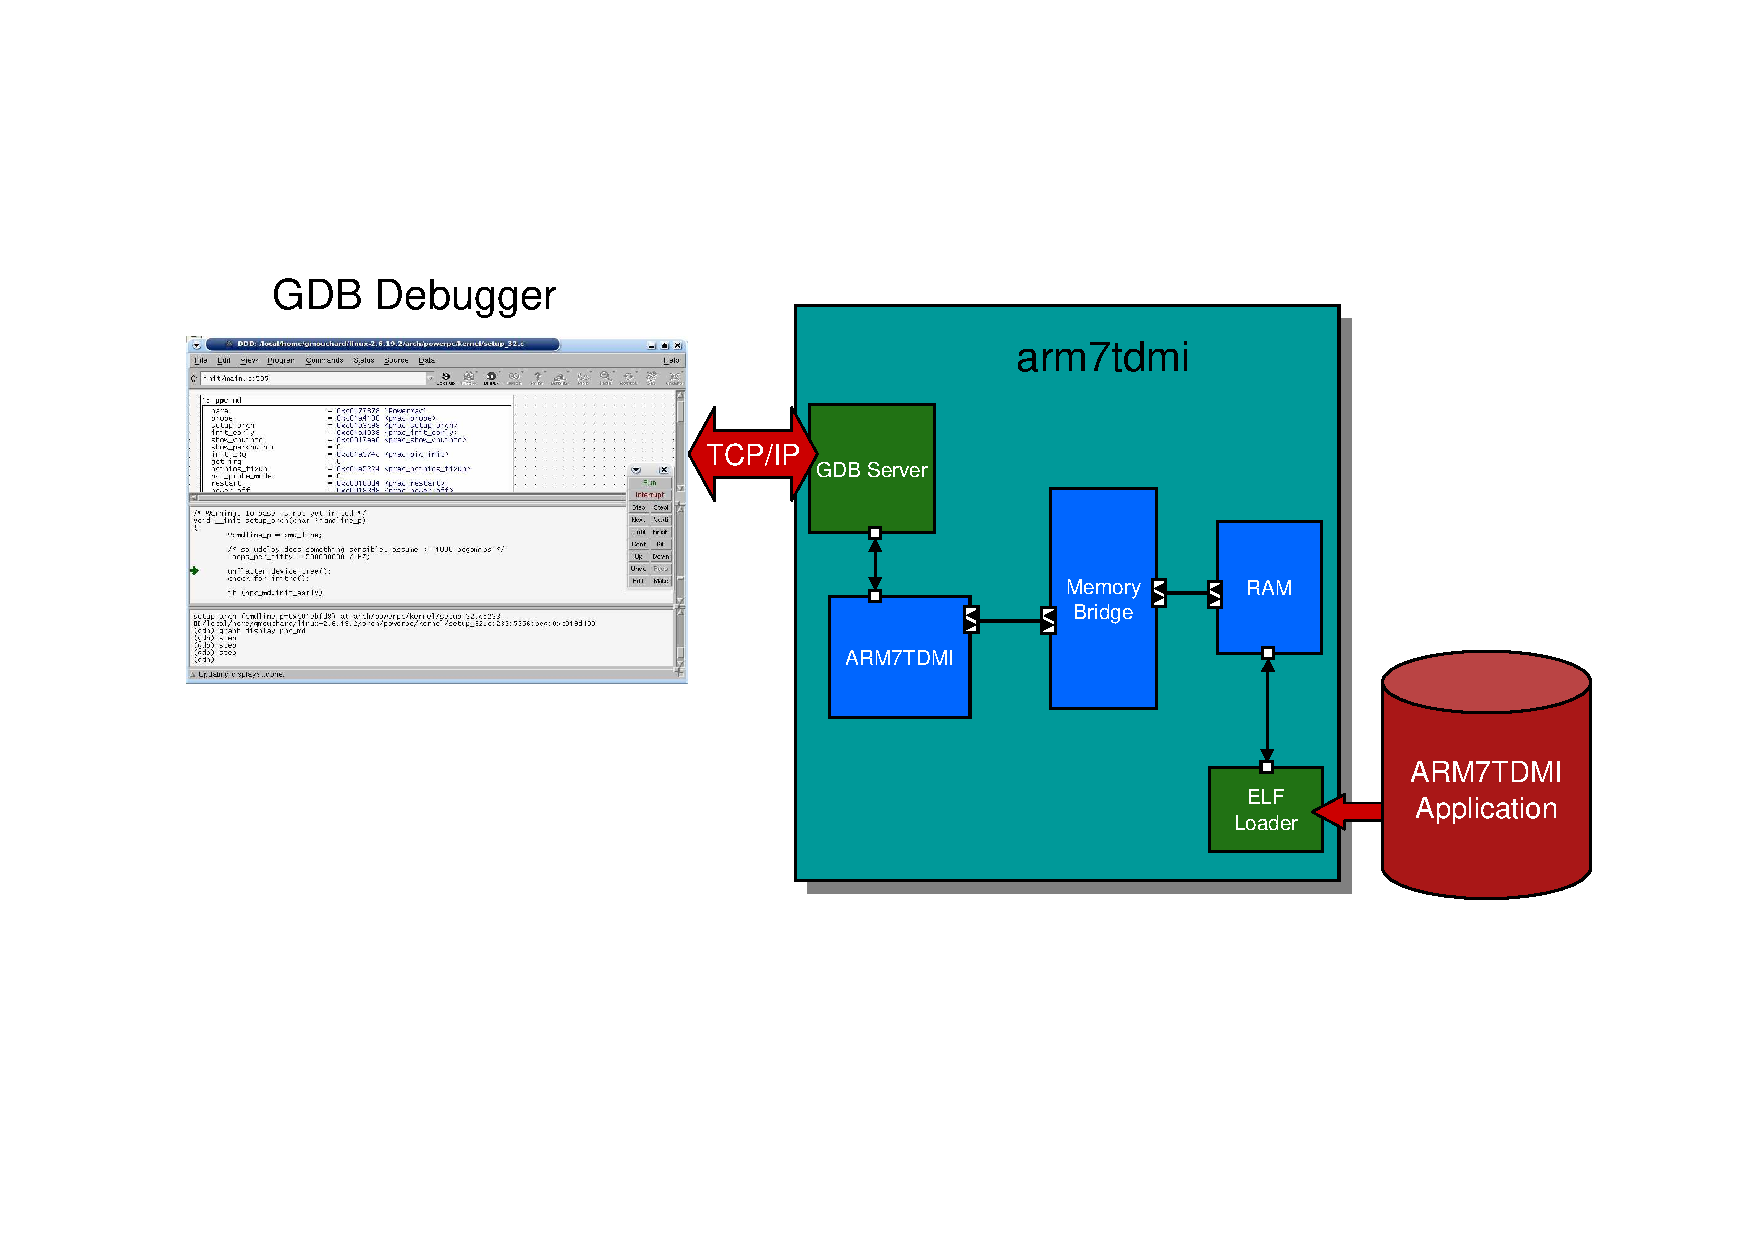
\includegraphics[width=\textwidth]{arm7tdmi/fig_arm7tdmi.pdf}
	\end{center}
	\caption{arm7tdmi simplified schematic.}
	\label{fig:arm7tdmi}
\end{figure}

Two different versions of the simulator are available:
\begin{itemize}
	\item arm7tdmi: the ARM7TDMI simulator
    \item arm7tdmi-debug: the ARM7TDMI simulator with debug information to see (traces) what is happening inside the simulator (note: it is slow)
\end{itemize}

\section{Simulated configuration}

The simulator is composed of the following modules:
\begin{itemize}\addtolength{\itemsep}{-0.40\baselineskip}
\item ARM CPU configured as an ARM7TDMI
\item Simple bus to memory bridge
\item memory
\end{itemize}

The simulator uses the following services:
\begin{itemize}\addtolength{\itemsep}{-0.40\baselineskip}
\item ELF loader
\item GDB Server
\item Inline debugger
\item SystemC Time
\item Host Time
\end{itemize}

\section{Using the simulator}

Usage: \texttt{arm7tdmi [<options>] <program> [program arguments]}

     'program' is statically linked ELF32 ARM Linux program

Options:
\begin{itemize}
\item Displaying the integrated help

\texttt{--help}
\texttt{-h}

\item Getting the simulation default configuration variables into a XML file\\
\texttt{--get-variables <xml file>}\\
\texttt{-v <xml file>}

\item Configuring the simulator with the given XML configuration file\\
\texttt{--config <xml file>}\\
\texttt{-c <xml file>}

\item Getting the simulator default configuration XML file\\
\texttt{--get-config <xml file>}\\
\texttt{-g <xml file>}\\

Note: you can use it as a template to create your own XML configuration file.

\item Activating the logger\\
\texttt{--logger}\\
\texttt{-l}

\item Defining the XML processor description file for GDB\\
\texttt{--xml-gdb <file>}\\
\texttt{-x <file>}

\item Activating the GDB server\\
\texttt{--gdb-server <port\_number>}\\
\texttt{-d <port\_number>}\\
           
Note: GDB server will use the given port\\

\item Activating the inline debugger\\
\texttt{--inline-debugger}\\
\texttt{-i}

\item Activating message spies\\
\texttt{--message-spy}\\
\texttt{-m}
\end{itemize}

The arm7tdmi simulator provides few options, but you can highly configure them using XML configuration file. To have a canvas of the XML configuration file simply run the simulator with the following option:
\begin{verbatim}
-g <xml file>
\end{verbatim}

This will generate an XML file describing the default configuration of the simulator. The following code shows you part of the initial xml configuration of the arm7tdmi:
\begin{verbatim}
<?xml version="1.0" encoding="UTF-8"?>
<VARIABLES>
  <variable>
    <type>parameter</type>
    <name>bridge.fsb-cycle-time</name>
    <data_type>unsigned long long</data_type>
    <default_value>0x0</default_value>
    <value>0x0</value>
    <description></description>
  </variable>
  <variable>
    <type>parameter</type>
    <name>bridge.mem-cycle-time</name>
    <data_type>unsigned long long</data_type>
    <default_value>0x0</default_value>
    <value>0x0</value>
    <description></description>
  </variable>
...
</VARIABLES>
\end{verbatim}

Modify the value field of the configuration parameters as you wish to set up your personal configuration, and use the -c option on the simulator to launch the simulation with your modified configuration file.


\chapter{arm966e\_s}
\label{arm966e_s}
\section{Introduction}

The arm966e\_s is a system level simulator of the ARM966E\_S processor. This simulator is a very simple simulator with just a memory connected to it. It is able to run any firmware loaded into the ram of the simulator, programs can use the full instruction set of those processors, including the Thumb instruction set. The simulator uses an elf binary loader to load into memory the firmware to simulate. Take into account that programs for those simulators require to be correctly mapped into the memory, refer to the processors manuals for more information. Software running on the simulated hardware can be debugged by connecting a GDB client to the simulator through the GDB serial remote protocol. The GDB client can be either the standard text based client (i.e. command gdb), a graphical front-end to GDB (e.g. ddd), or even Eclipse CDT. Additionally an inline debugger is also available.

The arm966e\_s does implement the CP15 coprocessor as described in the processor manual, and includes the integrated scratchpad memories (called TCM, tightly coupled memory). 

\begin{figure}[!h]
	\begin{center}
		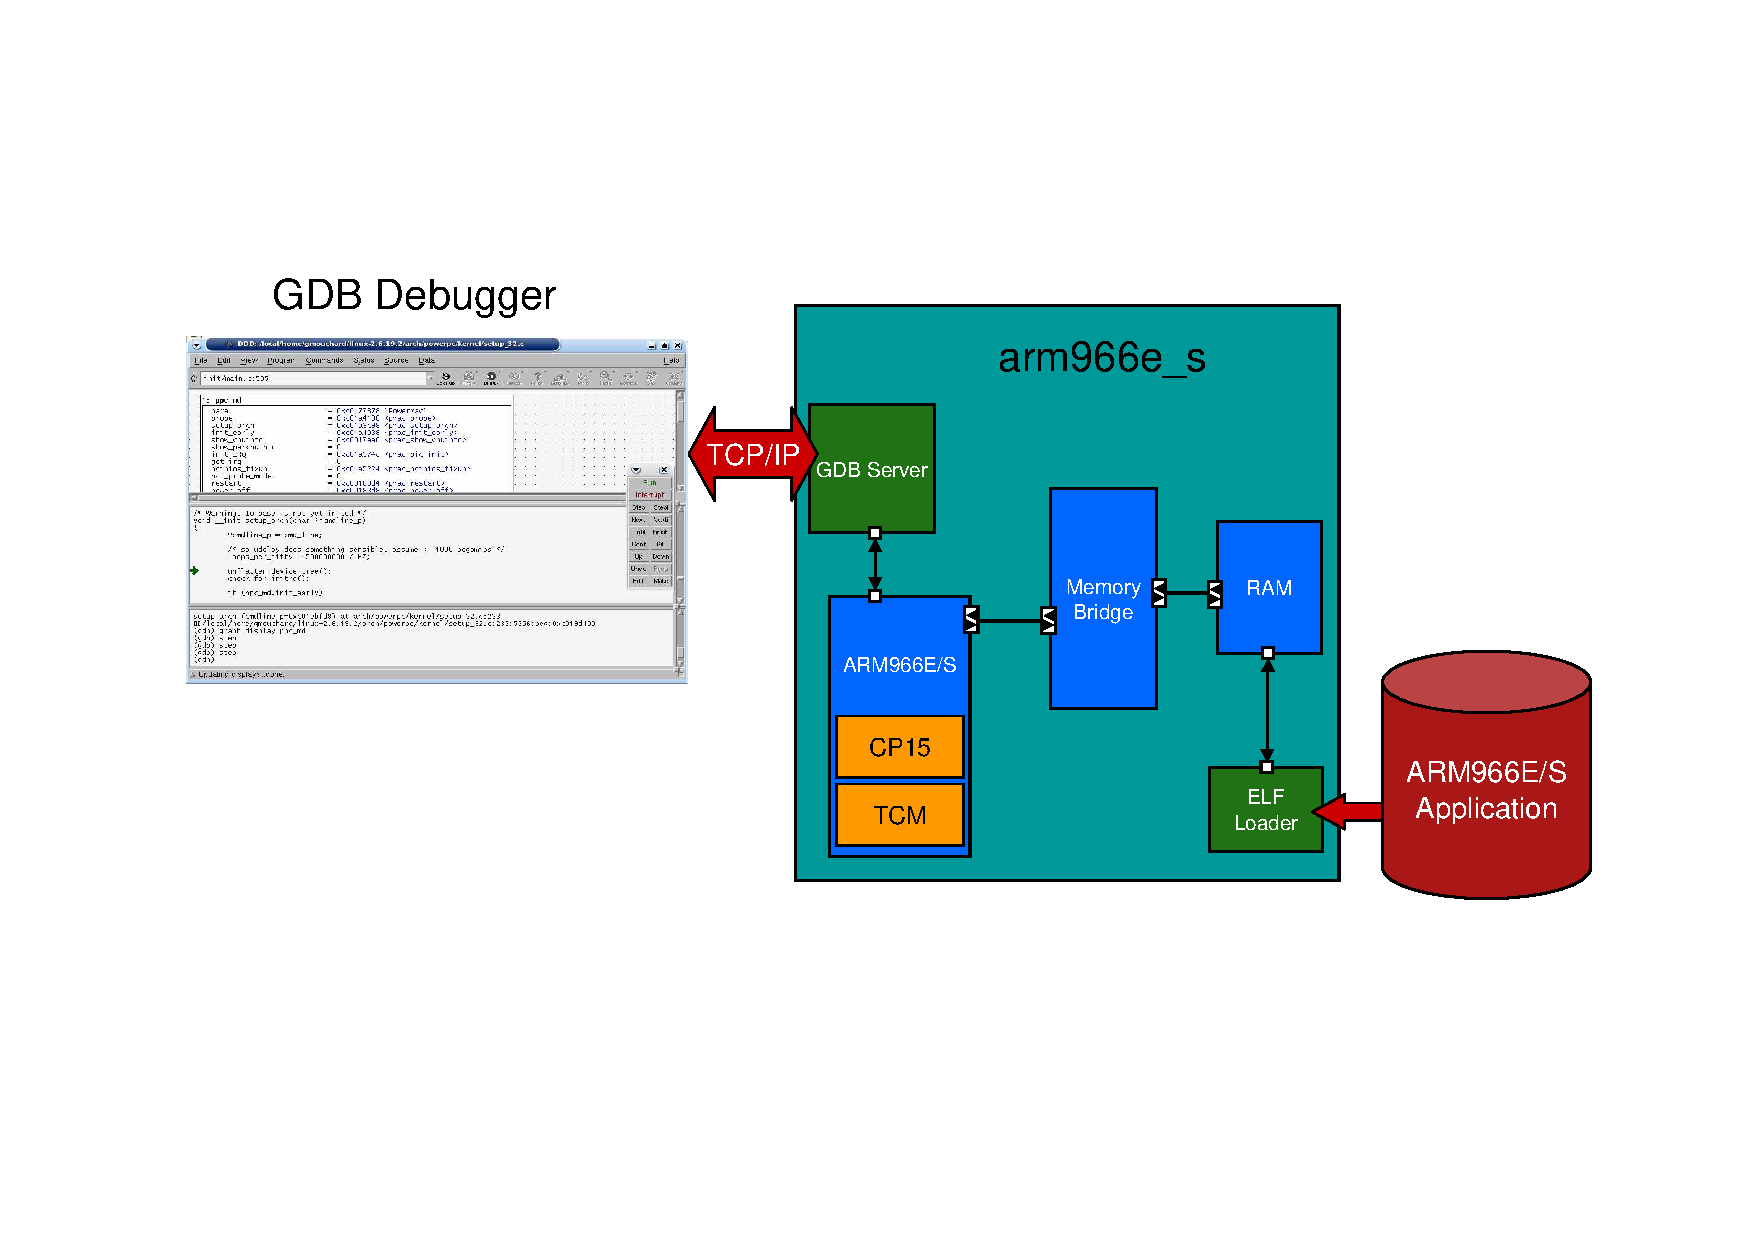
\includegraphics[width=\textwidth]{arm966e_s/fig_arm966e_s.pdf}
	\end{center}
	\caption{arm966e\_s simplified schematic.}
	\label{fig:arm966e_s}
\end{figure}

Two different versions of the simulator are available:
\begin{itemize}
	\item arm966e\_s: the ARM966E\_S simulator
    \item arm966e\_s-debug: the ARM966E\_S simulator with debug information to see (traces) what is happening inside the simulator (note: it is slow)
\end{itemize}

\section{Simulated configuration}

The simulator is composed of the following modules:
\begin{itemize}\addtolength{\itemsep}{-0.40\baselineskip}
\item ARM CPU configured as an ARM966E\_S
\item Simple bus to memory bridge
\item memory
\end{itemize}

The simulator uses the following services:
\begin{itemize}\addtolength{\itemsep}{-0.40\baselineskip}
\item ELF loader
\item GDB Server
\item Inline debugger
\item SystemC Time
\item Host Time
\end{itemize}

\section{Using the simulator}

Usage: \texttt{arm966e\_s [<options>] <program> [program arguments]}

     'program' is statically linked ELF32 ARM Linux program

Options:
\begin{itemize}
\item Displaying the integrated help

\texttt{--help}
\texttt{-h}

\item Getting the simulation default configuration variables into a XML file\\
\texttt{--get-variables <xml file>}\\
\texttt{-v <xml file>}

\item Configuring the simulator with the given XML configuration file\\
\texttt{--config <xml file>}\\
\texttt{-c <xml file>}

\item Getting the simulator default configuration XML file\\
\texttt{--get-config <xml file>}\\
\texttt{-g <xml file>}\\

Note: you can use it as a template to create your own XML configuration file.

\item Activating the logger\\
\texttt{--logger}\\
\texttt{-l}

\item Defining the XML processor description file for GDB\\
\texttt{--xml-gdb <file>}\\
\texttt{-x <file>}

\item Activating the GDB server\\
\texttt{--gdb-server <port\_number>}\\
\texttt{-d <port\_number>}\\
           
Note: GDB server will use the given port\\

\item Activating the inline debugger\\
\texttt{--inline-debugger}\\
\texttt{-i}

\item Activating message spies\\
\texttt{--message-spy}\\
\texttt{-m}
\end{itemize}

The arm966e\_s simulator provides few options, but you can highly configure them using XML configuration file. To have a canvas of the XML configuration file simply run the simulator with the following option:
\begin{verbatim}
-g <xml file>
\end{verbatim}

This will generate an XML file describing the default configuration of the simulator. The following code shows you part of the initial xml configuration of the arm966e\_s:
\begin{verbatim}
<?xml version="1.0" encoding="UTF-8"?>
<VARIABLES>
  <variable>
    <type>parameter</type>
    <name>bridge.fsb-cycle-time</name>
    <data_type>unsigned long long</data_type>
    <default_value>0x0</default_value>
    <value>0x0</value>
    <description></description>
  </variable>
  <variable>
    <type>parameter</type>
    <name>bridge.mem-cycle-time</name>
    <data_type>unsigned long long</data_type>
    <default_value>0x0</default_value>
    <value>0x0</value>
    <description></description>
  </variable>
...
</VARIABLES>
\end{verbatim}

Modify the value field of the configuration parameters as you wish to set up your personal configuration, and use the -c option on the simulator to launch the simulation with your modified configuration file.


\chapter{ppcemu}
\label{ppcemu}
This documentation has been automatically generated from the simulator \texttt{UNISIM ppcemu} version 1.0beta5 on Oct 23 2013.
\subsection{Introduction}
UNISIM ppcemu, user level PowerPC simulator with support of ELF32 binaries and Linux system call translation.\\
Section \ref{UNISIM ppcemu_licensing} gives licensing informations about the simulator.
Section \ref{UNISIM ppcemu_simulated_configuration} shows the set of modules and services that compose the simulator.
Section \ref{UNISIM ppcemu_using} shows how to invoke the simulator at the command line prompt.
Section \ref{UNISIM ppcemu_configuration} gives the simulator parameters.
Section \ref{UNISIM ppcemu_statistics} gives the simulator statistic counters.
Section \ref{UNISIM ppcemu_formulas} gives the simulator statistic formulas.
\subsection{Licensing}
\label{UNISIM ppcemu_licensing}
UNISIM ppcemu 1.0beta5\\
Copyright (C) 2007-2010, Commissariat a l'Energie Atomique (CEA)\\
License: BSD (see file COPYING)\\
Authors: Gilles Mouchard $<$gilles.mouchard@cea.fr$>$, Daniel Gracia P\'erez $<$daniel.gracia-perez@cea.fr$>$\\
\subsection{Simulated configuration}
\label{UNISIM ppcemu_simulated_configuration}
\begin{figure}[!ht]
	\begin{center}
		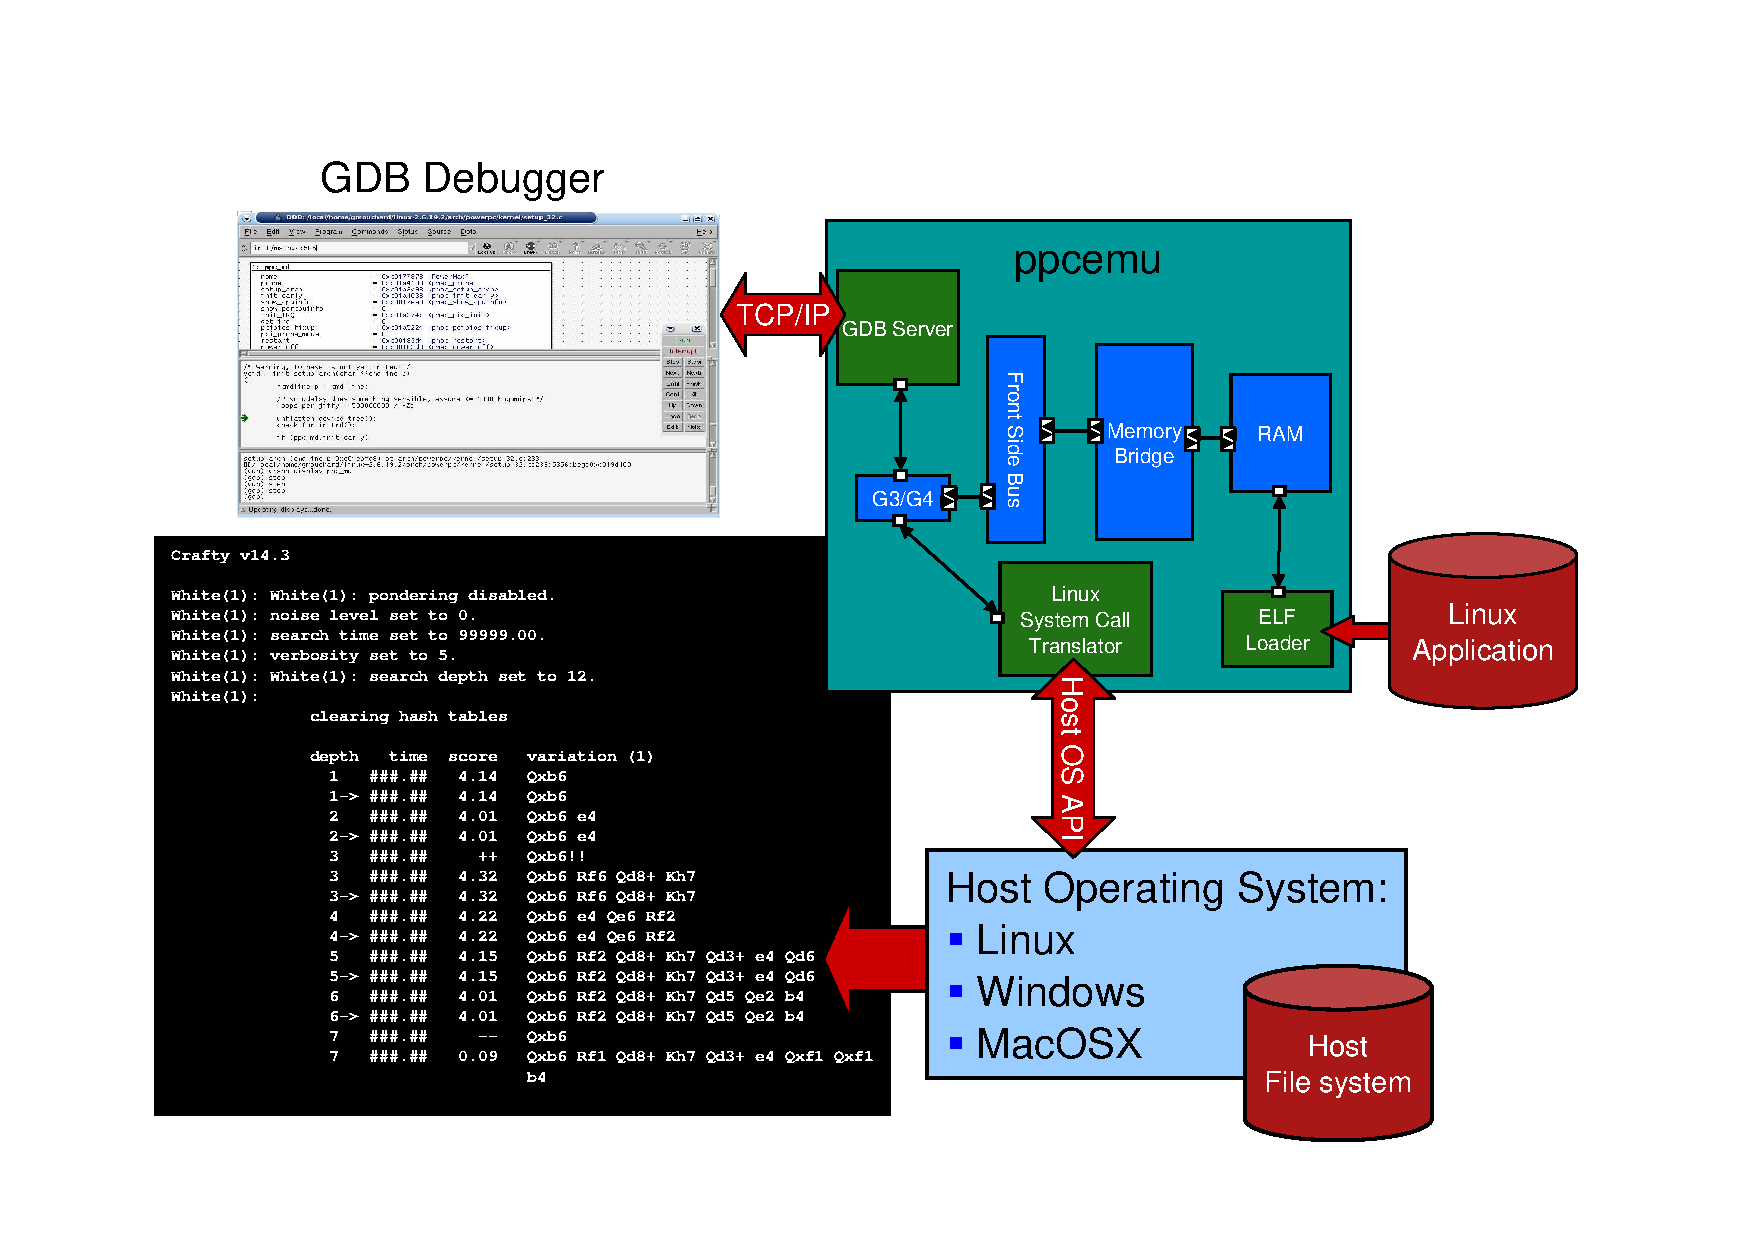
\includegraphics[width=\textwidth]{ppcemu/fig_schematic.pdf}
	\end{center}
	\caption{UNISIM ppcemu simulator schematic.}
\end{figure}
\noindent The UNISIM ppcemu simulator is composed of the following modules and services:
\begin{itemize}\addtolength{\itemsep}{-0.40\baselineskip}
\item \textbf{cpu}: this module implements a MPC7447A CPU core
\item \textbf{debugger}
\item \textbf{gdb-server}: this service implements the GDB server remote serial protocol over TCP/IP. Standards GDB clients (e.g. gdb, eclipse, ddd) can connect to the simulator to debug the target application that runs within the simulator.
\item \textbf{host-time}: this service is an abstraction layer for the host machine time
\item \textbf{inline-debugger}: this service implements a built-in debugger in the terminal console
\item \textbf{linux-os}
\item \textbf{memory}: this module implements a memory
\item \textbf{profiler}
\item \textbf{tee-memory-access-reporting}
\item \textbf{tee-memory-access-reporting.tee-memory-access-reporting.control\_selector[0]}
\item \textbf{tee-memory-access-reporting.tee-memory-access-reporting.control\_selector[10]}
\item \textbf{tee-memory-access-reporting.tee-memory-access-reporting.control\_selector[11]}
\item \textbf{tee-memory-access-reporting.tee-memory-access-reporting.control\_selector[12]}
\item \textbf{tee-memory-access-reporting.tee-memory-access-reporting.control\_selector[13]}
\item \textbf{tee-memory-access-reporting.tee-memory-access-reporting.control\_selector[14]}
\item \textbf{tee-memory-access-reporting.tee-memory-access-reporting.control\_selector[15]}
\item \textbf{tee-memory-access-reporting.tee-memory-access-reporting.control\_selector[1]}
\item \textbf{tee-memory-access-reporting.tee-memory-access-reporting.control\_selector[2]}
\item \textbf{tee-memory-access-reporting.tee-memory-access-reporting.control\_selector[3]}
\item \textbf{tee-memory-access-reporting.tee-memory-access-reporting.control\_selector[4]}
\item \textbf{tee-memory-access-reporting.tee-memory-access-reporting.control\_selector[5]}
\item \textbf{tee-memory-access-reporting.tee-memory-access-reporting.control\_selector[6]}
\item \textbf{tee-memory-access-reporting.tee-memory-access-reporting.control\_selector[7]}
\item \textbf{tee-memory-access-reporting.tee-memory-access-reporting.control\_selector[8]}
\item \textbf{tee-memory-access-reporting.tee-memory-access-reporting.control\_selector[9]}
\item \textbf{time}: this service is an abstraction layer for the SystemC kernel time
\end{itemize}
\subsection{Using the UNISIM ppcemu simulator}
\label{UNISIM ppcemu_using}
The UNISIM ppcemu simulator has the following command line options:\\
~\\
\noindent Usage: \texttt{unisim-ppcemu-1.0beta5 [<options>] [...]}

\noindent Options:
\begin{itemize}
\item \texttt{--set $<$param=value$>$ or -s $<$param=value$>$}: set value of parameter 'param' to 'value'
\item \texttt{--config $<$XML file$>$ or -c $<$XML file$>$}: configures the simulator with the given XML configuration file
\item \texttt{--get-config $<$XML file$>$ or -g $<$XML file$>$}: get the simulator configuration XML file (you can use it to create your own configuration. This option can be combined with -c to get a new configuration file with existing variables from another file
\item \texttt{--list or -l}: lists all available parameters, their type, and their current value
\item \texttt{--warn or -w}: enable printing of kernel warnings
\item \texttt{--doc $<$Latex file$>$ or -d $<$Latex file$>$}: enable printing a latex documentation
\item \texttt{--version or -v}: displays the program version information
\item \texttt{--share-path $<$path$>$ or -p $<$path$>$}: the path that should be used for the share directory (absolute path)
\item \texttt{--help or -h}: displays this help
\end{itemize}
\subsection{Configuration}
\label{UNISIM ppcemu_configuration}
Simulator configuration (see below) can be modified using command line Options \texttt{--set $<$param=value$>$} or \texttt{--config $<$config file$>$}.\\
~\\
\tablehead{\hline}
\tabletail{\hline}
\begin{supertabular}{|p{7.5cm}|p{7.5cm}|}
\multicolumn{2}{|l|}{\textbf{\Large Global}}\\
\hline
\multicolumn{1}{|p{7.5cm}}{\textbf{Name:} \texttt{enable-gdb-server}} & \multicolumn{1}{p{7.5cm}|}{\textbf{Type:} \texttt{parameter}}\\
\multicolumn{1}{|p{7.5cm}}{\textbf{Default:} \texttt{true}} & \multicolumn{1}{p{7.5cm}|}{\textbf{Data type:} \texttt{boolean}}\\
\multicolumn{2}{|p{15cm}|}{\textbf{Valid:} \texttt{true},~\texttt{false}}\\
\multicolumn{2}{|l|}{}\\
\multicolumn{2}{|p{15cm}|}{\textbf{Description:} \newline Enable/Disable GDB server instantiation.}\\
\hline
\multicolumn{1}{|p{7.5cm}}{\textbf{Name:} \texttt{enable-inline-debugger}} & \multicolumn{1}{p{7.5cm}|}{\textbf{Type:} \texttt{parameter}}\\
\multicolumn{1}{|p{7.5cm}}{\textbf{Default:} \texttt{true}} & \multicolumn{1}{p{7.5cm}|}{\textbf{Data type:} \texttt{boolean}}\\
\multicolumn{2}{|p{15cm}|}{\textbf{Valid:} \texttt{true},~\texttt{false}}\\
\multicolumn{2}{|l|}{}\\
\multicolumn{2}{|p{15cm}|}{\textbf{Description:} \newline Enable/Disable inline debugger instantiation.}\\
\hline
\multicolumn{1}{|p{7.5cm}}{\textbf{Name:} \texttt{enable-press-enter-at-exit}} & \multicolumn{1}{p{7.5cm}|}{\textbf{Type:} \texttt{parameter}}\\
\multicolumn{1}{|p{7.5cm}}{\textbf{Default:} \texttt{false}} & \multicolumn{1}{p{7.5cm}|}{\textbf{Data type:} \texttt{boolean}}\\
\multicolumn{2}{|p{15cm}|}{\textbf{Valid:} \texttt{true},~\texttt{false}}\\
\multicolumn{2}{|l|}{}\\
\multicolumn{2}{|p{15cm}|}{\textbf{Description:} \newline Enable/Disable pressing key enter at exit.}\\
\hline
\multicolumn{1}{|p{7.5cm}}{\textbf{Name:} \texttt{estimate-power}} & \multicolumn{1}{p{7.5cm}|}{\textbf{Type:} \texttt{parameter}}\\
\multicolumn{1}{|p{7.5cm}}{\textbf{Default:} \texttt{false}} & \multicolumn{1}{p{7.5cm}|}{\textbf{Data type:} \texttt{boolean}}\\
\multicolumn{2}{|p{15cm}|}{\textbf{Valid:} \texttt{true},~\texttt{false}}\\
\multicolumn{2}{|l|}{}\\
\multicolumn{2}{|p{15cm}|}{\textbf{Description:} \newline Enable/Disable power estimators instantiation.}\\
\hline
\multicolumn{1}{|p{7.5cm}}{\textbf{Name:} \texttt{kernel\_logger.file}} & \multicolumn{1}{p{7.5cm}|}{\textbf{Type:} \texttt{parameter}}\\
\multicolumn{1}{|p{7.5cm}}{\textbf{Default:} \texttt{false}} & \multicolumn{1}{p{7.5cm}|}{\textbf{Data type:} \texttt{boolean}}\\
\multicolumn{2}{|p{15cm}|}{\textbf{Valid:} \texttt{true},~\texttt{false}}\\
\multicolumn{2}{|l|}{}\\
\multicolumn{2}{|p{15cm}|}{\textbf{Description:} \newline Keep logger output in a file.}\\
\hline
\multicolumn{1}{|p{7.5cm}}{\textbf{Name:} \texttt{kernel\_logger.filename}} & \multicolumn{1}{p{7.5cm}|}{\textbf{Type:} \texttt{parameter}}\\
\multicolumn{1}{|p{7.5cm}}{\textbf{Default:} \texttt{logger\_output.txt}} & \multicolumn{1}{p{7.5cm}|}{\textbf{Data type:} \texttt{string}}\\
\multicolumn{2}{|l|}{}\\
\multicolumn{2}{|l|}{}\\
\multicolumn{2}{|p{15cm}|}{\textbf{Description:} \newline Filename to keep logger output \_(the option file must be activated).}\\
\hline
\multicolumn{1}{|p{7.5cm}}{\textbf{Name:} \texttt{kernel\_logger.std\_err}} & \multicolumn{1}{p{7.5cm}|}{\textbf{Type:} \texttt{parameter}}\\
\multicolumn{1}{|p{7.5cm}}{\textbf{Default:} \texttt{true}} & \multicolumn{1}{p{7.5cm}|}{\textbf{Data type:} \texttt{boolean}}\\
\multicolumn{2}{|p{15cm}|}{\textbf{Valid:} \texttt{true},~\texttt{false}}\\
\multicolumn{2}{|l|}{}\\
\multicolumn{2}{|p{15cm}|}{\textbf{Description:} \newline Show logger output through the standard error output.}\\
\hline
\multicolumn{1}{|p{7.5cm}}{\textbf{Name:} \texttt{kernel\_logger.std\_err\_color}} & \multicolumn{1}{p{7.5cm}|}{\textbf{Type:} \texttt{parameter}}\\
\multicolumn{1}{|p{7.5cm}}{\textbf{Default:} \texttt{false}} & \multicolumn{1}{p{7.5cm}|}{\textbf{Data type:} \texttt{boolean}}\\
\multicolumn{2}{|p{15cm}|}{\textbf{Valid:} \texttt{true},~\texttt{false}}\\
\multicolumn{2}{|l|}{}\\
\multicolumn{2}{|p{15cm}|}{\textbf{Description:} \newline Colorize logger output through the standard error output \_(only works if std\_err is active).}\\
\hline
\multicolumn{1}{|p{7.5cm}}{\textbf{Name:} \texttt{kernel\_logger.std\_out}} & \multicolumn{1}{p{7.5cm}|}{\textbf{Type:} \texttt{parameter}}\\
\multicolumn{1}{|p{7.5cm}}{\textbf{Default:} \texttt{false}} & \multicolumn{1}{p{7.5cm}|}{\textbf{Data type:} \texttt{boolean}}\\
\multicolumn{2}{|p{15cm}|}{\textbf{Valid:} \texttt{true},~\texttt{false}}\\
\multicolumn{2}{|l|}{}\\
\multicolumn{2}{|p{15cm}|}{\textbf{Description:} \newline Show logger output through the standard output.}\\
\hline
\multicolumn{1}{|p{7.5cm}}{\textbf{Name:} \texttt{kernel\_logger.std\_out\_color}} & \multicolumn{1}{p{7.5cm}|}{\textbf{Type:} \texttt{parameter}}\\
\multicolumn{1}{|p{7.5cm}}{\textbf{Default:} \texttt{false}} & \multicolumn{1}{p{7.5cm}|}{\textbf{Data type:} \texttt{boolean}}\\
\multicolumn{2}{|p{15cm}|}{\textbf{Valid:} \texttt{true},~\texttt{false}}\\
\multicolumn{2}{|l|}{}\\
\multicolumn{2}{|p{15cm}|}{\textbf{Description:} \newline Colorize logger output through the standard output \_(only works if std\_out is active).}\\
\hline
\multicolumn{1}{|p{7.5cm}}{\textbf{Name:} \texttt{kernel\_logger.xml\_file}} & \multicolumn{1}{p{7.5cm}|}{\textbf{Type:} \texttt{parameter}}\\
\multicolumn{1}{|p{7.5cm}}{\textbf{Default:} \texttt{false}} & \multicolumn{1}{p{7.5cm}|}{\textbf{Data type:} \texttt{boolean}}\\
\multicolumn{2}{|p{15cm}|}{\textbf{Valid:} \texttt{true},~\texttt{false}}\\
\multicolumn{2}{|l|}{}\\
\multicolumn{2}{|p{15cm}|}{\textbf{Description:} \newline Keep logger output in a file xml formatted.}\\
\hline
\multicolumn{1}{|p{7.5cm}}{\textbf{Name:} \texttt{kernel\_logger.xml\_file\_gzipped}} & \multicolumn{1}{p{7.5cm}|}{\textbf{Type:} \texttt{parameter}}\\
\multicolumn{1}{|p{7.5cm}}{\textbf{Default:} \texttt{false}} & \multicolumn{1}{p{7.5cm}|}{\textbf{Data type:} \texttt{boolean}}\\
\multicolumn{2}{|p{15cm}|}{\textbf{Valid:} \texttt{true},~\texttt{false}}\\
\multicolumn{2}{|l|}{}\\
\multicolumn{2}{|p{15cm}|}{\textbf{Description:} \newline If the xml\_file option is active, the output file will be compressed (a .gz extension will be automatically added to the xml\_filename option.}\\
\hline
\multicolumn{1}{|p{7.5cm}}{\textbf{Name:} \texttt{kernel\_logger.xml\_filename}} & \multicolumn{1}{p{7.5cm}|}{\textbf{Type:} \texttt{parameter}}\\
\multicolumn{1}{|p{7.5cm}}{\textbf{Default:} \texttt{logger\_output.xml}} & \multicolumn{1}{p{7.5cm}|}{\textbf{Data type:} \texttt{string}}\\
\multicolumn{2}{|l|}{}\\
\multicolumn{2}{|l|}{}\\
\multicolumn{2}{|p{15cm}|}{\textbf{Description:} \newline Filename to keep logger xml output \_(the option xml\_file must be activated).}\\
\hline
\hline
\multicolumn{2}{|l|}{\textbf{\Large cpu}}\\
\hline
\multicolumn{1}{|p{7.5cm}}{\textbf{Name:} \texttt{cpu.cpu-cycle-time}} & \multicolumn{1}{p{7.5cm}|}{\textbf{Type:} \texttt{parameter}}\\
\multicolumn{1}{|p{7.5cm}}{\textbf{Default:} \texttt{3333}} & \multicolumn{1}{p{7.5cm}|}{\textbf{Data type:} \texttt{unsigned 64-bit integer}}\\
\multicolumn{2}{|l|}{}\\
\multicolumn{2}{|l|}{}\\
\multicolumn{2}{|p{15cm}|}{\textbf{Description:} \newline CPU cycle time in picoseconds.}\\
\hline
\multicolumn{1}{|p{7.5cm}}{\textbf{Name:} \texttt{cpu.voltage}} & \multicolumn{1}{p{7.5cm}|}{\textbf{Type:} \texttt{parameter}}\\
\multicolumn{1}{|p{7.5cm}}{\textbf{Default:} \texttt{1300}} & \multicolumn{1}{p{7.5cm}|}{\textbf{Data type:} \texttt{unsigned 64-bit integer}}\\
\multicolumn{2}{|l|}{}\\
\multicolumn{2}{|l|}{}\\
\multicolumn{2}{|p{15cm}|}{\textbf{Description:} \newline CPU voltage in mV.}\\
\hline
\multicolumn{1}{|p{7.5cm}}{\textbf{Name:} \texttt{cpu.max-inst}} & \multicolumn{1}{p{7.5cm}|}{\textbf{Type:} \texttt{parameter}}\\
\multicolumn{1}{|p{7.5cm}}{\textbf{Default:} \texttt{18446744073709551615}} & \multicolumn{1}{p{7.5cm}|}{\textbf{Data type:} \texttt{unsigned 64-bit integer}}\\
\multicolumn{2}{|l|}{}\\
\multicolumn{2}{|l|}{}\\
\multicolumn{2}{|p{15cm}|}{\textbf{Description:} \newline maximum number of instructions to simulate.}\\
\hline
\multicolumn{1}{|p{7.5cm}}{\textbf{Name:} \texttt{cpu.verbose-all}} & \multicolumn{1}{p{7.5cm}|}{\textbf{Type:} \texttt{parameter}}\\
\multicolumn{1}{|p{7.5cm}}{\textbf{Default:} \texttt{false}} & \multicolumn{1}{p{7.5cm}|}{\textbf{Data type:} \texttt{boolean}}\\
\multicolumn{2}{|p{15cm}|}{\textbf{Valid:} \texttt{true},~\texttt{false}}\\
\multicolumn{2}{|l|}{}\\
\multicolumn{2}{|p{15cm}|}{\textbf{Description:} \newline globally enable/disable verbosity.}\\
\hline
\multicolumn{1}{|p{7.5cm}}{\textbf{Name:} \texttt{cpu.verbose-setup}} & \multicolumn{1}{p{7.5cm}|}{\textbf{Type:} \texttt{parameter}}\\
\multicolumn{1}{|p{7.5cm}}{\textbf{Default:} \texttt{false}} & \multicolumn{1}{p{7.5cm}|}{\textbf{Data type:} \texttt{boolean}}\\
\multicolumn{2}{|p{15cm}|}{\textbf{Valid:} \texttt{true},~\texttt{false}}\\
\multicolumn{2}{|l|}{}\\
\multicolumn{2}{|p{15cm}|}{\textbf{Description:} \newline enable/disable verbosity while setup.}\\
\hline
\multicolumn{1}{|p{7.5cm}}{\textbf{Name:} \texttt{cpu.verbose-step}} & \multicolumn{1}{p{7.5cm}|}{\textbf{Type:} \texttt{parameter}}\\
\multicolumn{1}{|p{7.5cm}}{\textbf{Default:} \texttt{false}} & \multicolumn{1}{p{7.5cm}|}{\textbf{Data type:} \texttt{boolean}}\\
\multicolumn{2}{|p{15cm}|}{\textbf{Valid:} \texttt{true},~\texttt{false}}\\
\multicolumn{2}{|l|}{}\\
\multicolumn{2}{|p{15cm}|}{\textbf{Description:} \newline enable/disable verbosity when simulating an instruction.}\\
\hline
\multicolumn{1}{|p{7.5cm}}{\textbf{Name:} \texttt{cpu.verbose-dtlb}} & \multicolumn{1}{p{7.5cm}|}{\textbf{Type:} \texttt{parameter}}\\
\multicolumn{1}{|p{7.5cm}}{\textbf{Default:} \texttt{false}} & \multicolumn{1}{p{7.5cm}|}{\textbf{Data type:} \texttt{boolean}}\\
\multicolumn{2}{|p{15cm}|}{\textbf{Valid:} \texttt{true},~\texttt{false}}\\
\multicolumn{2}{|l|}{}\\
\multicolumn{2}{|p{15cm}|}{\textbf{Description:} \newline enable/disable verbosity when accessing data translation lookahead buffer.}\\
\hline
\multicolumn{1}{|p{7.5cm}}{\textbf{Name:} \texttt{cpu.verbose-itlb}} & \multicolumn{1}{p{7.5cm}|}{\textbf{Type:} \texttt{parameter}}\\
\multicolumn{1}{|p{7.5cm}}{\textbf{Default:} \texttt{false}} & \multicolumn{1}{p{7.5cm}|}{\textbf{Data type:} \texttt{boolean}}\\
\multicolumn{2}{|p{15cm}|}{\textbf{Valid:} \texttt{true},~\texttt{false}}\\
\multicolumn{2}{|l|}{}\\
\multicolumn{2}{|p{15cm}|}{\textbf{Description:} \newline enable/disable verbosity when accessing instruction translation lookahead buffer.}\\
\hline
\multicolumn{1}{|p{7.5cm}}{\textbf{Name:} \texttt{cpu.verbose-dl1}} & \multicolumn{1}{p{7.5cm}|}{\textbf{Type:} \texttt{parameter}}\\
\multicolumn{1}{|p{7.5cm}}{\textbf{Default:} \texttt{false}} & \multicolumn{1}{p{7.5cm}|}{\textbf{Data type:} \texttt{boolean}}\\
\multicolumn{2}{|p{15cm}|}{\textbf{Valid:} \texttt{true},~\texttt{false}}\\
\multicolumn{2}{|l|}{}\\
\multicolumn{2}{|p{15cm}|}{\textbf{Description:} \newline enable/disable verbosity when accessing L1 data cache.}\\
\hline
\multicolumn{1}{|p{7.5cm}}{\textbf{Name:} \texttt{cpu.verbose-il1}} & \multicolumn{1}{p{7.5cm}|}{\textbf{Type:} \texttt{parameter}}\\
\multicolumn{1}{|p{7.5cm}}{\textbf{Default:} \texttt{false}} & \multicolumn{1}{p{7.5cm}|}{\textbf{Data type:} \texttt{boolean}}\\
\multicolumn{2}{|p{15cm}|}{\textbf{Valid:} \texttt{true},~\texttt{false}}\\
\multicolumn{2}{|l|}{}\\
\multicolumn{2}{|p{15cm}|}{\textbf{Description:} \newline enable/disable verbosity when accessing L1 instruction cache.}\\
\hline
\multicolumn{1}{|p{7.5cm}}{\textbf{Name:} \texttt{cpu.verbose-l2}} & \multicolumn{1}{p{7.5cm}|}{\textbf{Type:} \texttt{parameter}}\\
\multicolumn{1}{|p{7.5cm}}{\textbf{Default:} \texttt{false}} & \multicolumn{1}{p{7.5cm}|}{\textbf{Data type:} \texttt{boolean}}\\
\multicolumn{2}{|p{15cm}|}{\textbf{Valid:} \texttt{true},~\texttt{false}}\\
\multicolumn{2}{|l|}{}\\
\multicolumn{2}{|p{15cm}|}{\textbf{Description:} \newline enable/disable verbosity when accessing L2 unified cache.}\\
\hline
\multicolumn{1}{|p{7.5cm}}{\textbf{Name:} \texttt{cpu.verbose-load}} & \multicolumn{1}{p{7.5cm}|}{\textbf{Type:} \texttt{parameter}}\\
\multicolumn{1}{|p{7.5cm}}{\textbf{Default:} \texttt{false}} & \multicolumn{1}{p{7.5cm}|}{\textbf{Data type:} \texttt{boolean}}\\
\multicolumn{2}{|p{15cm}|}{\textbf{Valid:} \texttt{true},~\texttt{false}}\\
\multicolumn{2}{|l|}{}\\
\multicolumn{2}{|p{15cm}|}{\textbf{Description:} \newline enable/disable verbosity when simulating a load.}\\
\hline
\multicolumn{1}{|p{7.5cm}}{\textbf{Name:} \texttt{cpu.verbose-store}} & \multicolumn{1}{p{7.5cm}|}{\textbf{Type:} \texttt{parameter}}\\
\multicolumn{1}{|p{7.5cm}}{\textbf{Default:} \texttt{false}} & \multicolumn{1}{p{7.5cm}|}{\textbf{Data type:} \texttt{boolean}}\\
\multicolumn{2}{|p{15cm}|}{\textbf{Valid:} \texttt{true},~\texttt{false}}\\
\multicolumn{2}{|l|}{}\\
\multicolumn{2}{|p{15cm}|}{\textbf{Description:} \newline enable/disable verbosity when simulating a store.}\\
\hline
\multicolumn{1}{|p{7.5cm}}{\textbf{Name:} \texttt{cpu.verbose-read-memory}} & \multicolumn{1}{p{7.5cm}|}{\textbf{Type:} \texttt{parameter}}\\
\multicolumn{1}{|p{7.5cm}}{\textbf{Default:} \texttt{false}} & \multicolumn{1}{p{7.5cm}|}{\textbf{Data type:} \texttt{boolean}}\\
\multicolumn{2}{|p{15cm}|}{\textbf{Valid:} \texttt{true},~\texttt{false}}\\
\multicolumn{2}{|l|}{}\\
\multicolumn{2}{|p{15cm}|}{\textbf{Description:} \newline enable/disable verbosity when reading memory for a debug purpose.}\\
\hline
\multicolumn{1}{|p{7.5cm}}{\textbf{Name:} \texttt{cpu.verbose-write-memory}} & \multicolumn{1}{p{7.5cm}|}{\textbf{Type:} \texttt{parameter}}\\
\multicolumn{1}{|p{7.5cm}}{\textbf{Default:} \texttt{false}} & \multicolumn{1}{p{7.5cm}|}{\textbf{Data type:} \texttt{boolean}}\\
\multicolumn{2}{|p{15cm}|}{\textbf{Valid:} \texttt{true},~\texttt{false}}\\
\multicolumn{2}{|l|}{}\\
\multicolumn{2}{|p{15cm}|}{\textbf{Description:} \newline enable/disable verbosity when writing memory for a debug purpose.}\\
\hline
\multicolumn{1}{|p{7.5cm}}{\textbf{Name:} \texttt{cpu.verbose-exception}} & \multicolumn{1}{p{7.5cm}|}{\textbf{Type:} \texttt{parameter}}\\
\multicolumn{1}{|p{7.5cm}}{\textbf{Default:} \texttt{false}} & \multicolumn{1}{p{7.5cm}|}{\textbf{Data type:} \texttt{boolean}}\\
\multicolumn{2}{|p{15cm}|}{\textbf{Valid:} \texttt{true},~\texttt{false}}\\
\multicolumn{2}{|l|}{}\\
\multicolumn{2}{|p{15cm}|}{\textbf{Description:} \newline enable/disable verbosity when handling exceptions.}\\
\hline
\multicolumn{1}{|p{7.5cm}}{\textbf{Name:} \texttt{cpu.verbose-set-msr}} & \multicolumn{1}{p{7.5cm}|}{\textbf{Type:} \texttt{parameter}}\\
\multicolumn{1}{|p{7.5cm}}{\textbf{Default:} \texttt{false}} & \multicolumn{1}{p{7.5cm}|}{\textbf{Data type:} \texttt{boolean}}\\
\multicolumn{2}{|p{15cm}|}{\textbf{Valid:} \texttt{true},~\texttt{false}}\\
\multicolumn{2}{|l|}{}\\
\multicolumn{2}{|p{15cm}|}{\textbf{Description:} \newline enable/disable verbosity when setting MSR.}\\
\hline
\multicolumn{1}{|p{7.5cm}}{\textbf{Name:} \texttt{cpu.verbose-set-hid0}} & \multicolumn{1}{p{7.5cm}|}{\textbf{Type:} \texttt{parameter}}\\
\multicolumn{1}{|p{7.5cm}}{\textbf{Default:} \texttt{false}} & \multicolumn{1}{p{7.5cm}|}{\textbf{Data type:} \texttt{boolean}}\\
\multicolumn{2}{|p{15cm}|}{\textbf{Valid:} \texttt{true},~\texttt{false}}\\
\multicolumn{2}{|l|}{}\\
\multicolumn{2}{|p{15cm}|}{\textbf{Description:} \newline enable/disable verbosity when setting HID0.}\\
\hline
\multicolumn{1}{|p{7.5cm}}{\textbf{Name:} \texttt{cpu.verbose-set-hid1}} & \multicolumn{1}{p{7.5cm}|}{\textbf{Type:} \texttt{parameter}}\\
\multicolumn{1}{|p{7.5cm}}{\textbf{Default:} \texttt{false}} & \multicolumn{1}{p{7.5cm}|}{\textbf{Data type:} \texttt{boolean}}\\
\multicolumn{2}{|p{15cm}|}{\textbf{Valid:} \texttt{true},~\texttt{false}}\\
\multicolumn{2}{|l|}{}\\
\multicolumn{2}{|p{15cm}|}{\textbf{Description:} \newline enable/disable verbosity when setting HID1.}\\
\hline
\multicolumn{1}{|p{7.5cm}}{\textbf{Name:} \texttt{cpu.verbose-set-hid2}} & \multicolumn{1}{p{7.5cm}|}{\textbf{Type:} \texttt{parameter}}\\
\multicolumn{1}{|p{7.5cm}}{\textbf{Default:} \texttt{false}} & \multicolumn{1}{p{7.5cm}|}{\textbf{Data type:} \texttt{boolean}}\\
\multicolumn{2}{|p{15cm}|}{\textbf{Valid:} \texttt{true},~\texttt{false}}\\
\multicolumn{2}{|l|}{}\\
\multicolumn{2}{|p{15cm}|}{\textbf{Description:} \newline enable/disable verbosity when setting HID2.}\\
\hline
\multicolumn{1}{|p{7.5cm}}{\textbf{Name:} \texttt{cpu.verbose-set-l2cr}} & \multicolumn{1}{p{7.5cm}|}{\textbf{Type:} \texttt{parameter}}\\
\multicolumn{1}{|p{7.5cm}}{\textbf{Default:} \texttt{false}} & \multicolumn{1}{p{7.5cm}|}{\textbf{Data type:} \texttt{boolean}}\\
\multicolumn{2}{|p{15cm}|}{\textbf{Valid:} \texttt{true},~\texttt{false}}\\
\multicolumn{2}{|l|}{}\\
\multicolumn{2}{|p{15cm}|}{\textbf{Description:} \newline enable/disable verbosity when setting L2CR.}\\
\hline
\multicolumn{1}{|p{7.5cm}}{\textbf{Name:} \texttt{cpu.enable-linux-printk-snooping}} & \multicolumn{1}{p{7.5cm}|}{\textbf{Type:} \texttt{parameter}}\\
\multicolumn{1}{|p{7.5cm}}{\textbf{Default:} \texttt{false}} & \multicolumn{1}{p{7.5cm}|}{\textbf{Data type:} \texttt{boolean}}\\
\multicolumn{2}{|p{15cm}|}{\textbf{Valid:} \texttt{true},~\texttt{false}}\\
\multicolumn{2}{|l|}{}\\
\multicolumn{2}{|p{15cm}|}{\textbf{Description:} \newline enable/disable linux printk buffer snooping.}\\
\hline
\multicolumn{1}{|p{7.5cm}}{\textbf{Name:} \texttt{cpu.enable-linux-syscall-snooping}} & \multicolumn{1}{p{7.5cm}|}{\textbf{Type:} \texttt{parameter}}\\
\multicolumn{1}{|p{7.5cm}}{\textbf{Default:} \texttt{false}} & \multicolumn{1}{p{7.5cm}|}{\textbf{Data type:} \texttt{boolean}}\\
\multicolumn{2}{|p{15cm}|}{\textbf{Valid:} \texttt{true},~\texttt{false}}\\
\multicolumn{2}{|l|}{}\\
\multicolumn{2}{|p{15cm}|}{\textbf{Description:} \newline enable/disable linux syscall snooping.}\\
\hline
\multicolumn{1}{|p{7.5cm}}{\textbf{Name:} \texttt{cpu.trap-on-instruction-counter}} & \multicolumn{1}{p{7.5cm}|}{\textbf{Type:} \texttt{parameter}}\\
\multicolumn{1}{|p{7.5cm}}{\textbf{Default:} \texttt{18446744073709551615}} & \multicolumn{1}{p{7.5cm}|}{\textbf{Data type:} \texttt{unsigned 64-bit integer}}\\
\multicolumn{2}{|l|}{}\\
\multicolumn{2}{|l|}{}\\
\multicolumn{2}{|p{15cm}|}{\textbf{Description:} \newline number of simulated instruction before traping.}\\
\hline
\multicolumn{1}{|p{7.5cm}}{\textbf{Name:} \texttt{cpu.halt-on}} & \multicolumn{1}{p{7.5cm}|}{\textbf{Type:} \texttt{parameter}}\\
\multicolumn{1}{|p{7.5cm}}{\textbf{Default:} \texttt{}} & \multicolumn{1}{p{7.5cm}|}{\textbf{Data type:} \texttt{string}}\\
\multicolumn{2}{|l|}{}\\
\multicolumn{2}{|l|}{}\\
\multicolumn{2}{|p{15cm}|}{\textbf{Description:} \newline Symbol or address where to stop simulation.}\\
\hline
\multicolumn{1}{|p{7.5cm}}{\textbf{Name:} \texttt{cpu.bus-cycle-time}} & \multicolumn{1}{p{7.5cm}|}{\textbf{Type:} \texttt{parameter}}\\
\multicolumn{1}{|p{7.5cm}}{\textbf{Default:} \texttt{13333 ps}} & \multicolumn{1}{p{7.5cm}|}{\textbf{Data type:} \texttt{sc\_time}}\\
\multicolumn{2}{|l|}{}\\
\multicolumn{2}{|l|}{}\\
\multicolumn{2}{|p{15cm}|}{\textbf{Description:} \newline bus cycle time.}\\
\hline
\multicolumn{1}{|p{7.5cm}}{\textbf{Name:} \texttt{cpu.nice-time}} & \multicolumn{1}{p{7.5cm}|}{\textbf{Type:} \texttt{parameter}}\\
\multicolumn{1}{|p{7.5cm}}{\textbf{Default:} \texttt{1 ms}} & \multicolumn{1}{p{7.5cm}|}{\textbf{Data type:} \texttt{sc\_time}}\\
\multicolumn{2}{|l|}{}\\
\multicolumn{2}{|l|}{}\\
\multicolumn{2}{|p{15cm}|}{\textbf{Description:} \newline maximum time between synchonizations.}\\
\hline
\multicolumn{1}{|p{7.5cm}}{\textbf{Name:} \texttt{cpu.ipc}} & \multicolumn{1}{p{7.5cm}|}{\textbf{Type:} \texttt{parameter}}\\
\multicolumn{1}{|p{7.5cm}}{\textbf{Default:} \texttt{1}} & \multicolumn{1}{p{7.5cm}|}{\textbf{Data type:} \texttt{double precision floating-point}}\\
\multicolumn{2}{|l|}{}\\
\multicolumn{2}{|l|}{}\\
\multicolumn{2}{|p{15cm}|}{\textbf{Description:} \newline maximum instructions per cycle (should be $<$= 2.0).}\\
\hline
\multicolumn{1}{|p{7.5cm}}{\textbf{Name:} \texttt{cpu.enable-host-idle}} & \multicolumn{1}{p{7.5cm}|}{\textbf{Type:} \texttt{parameter}}\\
\multicolumn{1}{|p{7.5cm}}{\textbf{Default:} \texttt{false}} & \multicolumn{1}{p{7.5cm}|}{\textbf{Data type:} \texttt{boolean}}\\
\multicolumn{2}{|p{15cm}|}{\textbf{Valid:} \texttt{true},~\texttt{false}}\\
\multicolumn{2}{|l|}{}\\
\multicolumn{2}{|p{15cm}|}{\textbf{Description:} \newline Enable/Disable host idle periods when target is idle.}\\
\hline
\multicolumn{1}{|p{7.5cm}}{\textbf{Name:} \texttt{cpu.enable-dmi}} & \multicolumn{1}{p{7.5cm}|}{\textbf{Type:} \texttt{parameter}}\\
\multicolumn{1}{|p{7.5cm}}{\textbf{Default:} \texttt{true}} & \multicolumn{1}{p{7.5cm}|}{\textbf{Data type:} \texttt{boolean}}\\
\multicolumn{2}{|p{15cm}|}{\textbf{Valid:} \texttt{true},~\texttt{false}}\\
\multicolumn{2}{|l|}{}\\
\multicolumn{2}{|p{15cm}|}{\textbf{Description:} \newline Enable/Disable TLM 2.0 DMI (Direct Memory Access) to speed-up simulation.}\\
\hline
\multicolumn{1}{|p{7.5cm}}{\textbf{Name:} \texttt{cpu.debug-dmi}} & \multicolumn{1}{p{7.5cm}|}{\textbf{Type:} \texttt{parameter}}\\
\multicolumn{1}{|p{7.5cm}}{\textbf{Default:} \texttt{false}} & \multicolumn{1}{p{7.5cm}|}{\textbf{Data type:} \texttt{boolean}}\\
\multicolumn{2}{|p{15cm}|}{\textbf{Valid:} \texttt{true},~\texttt{false}}\\
\multicolumn{2}{|l|}{}\\
\multicolumn{2}{|p{15cm}|}{\textbf{Description:} \newline Enable/Disable debugging of DMI (Direct Memory Access).}\\
\hline
\hline
\multicolumn{2}{|l|}{\textbf{\Large debugger}}\\
\hline
\multicolumn{1}{|p{7.5cm}}{\textbf{Name:} \texttt{debugger.verbose}} & \multicolumn{1}{p{7.5cm}|}{\textbf{Type:} \texttt{parameter}}\\
\multicolumn{1}{|p{7.5cm}}{\textbf{Default:} \texttt{false}} & \multicolumn{1}{p{7.5cm}|}{\textbf{Data type:} \texttt{boolean}}\\
\multicolumn{2}{|p{15cm}|}{\textbf{Valid:} \texttt{true},~\texttt{false}}\\
\multicolumn{2}{|l|}{}\\
\multicolumn{2}{|p{15cm}|}{\textbf{Description:} \newline Enable/Disable verbosity.}\\
\hline
\multicolumn{1}{|p{7.5cm}}{\textbf{Name:} \texttt{debugger.dwarf-to-html-output-} \newline$\hookrightarrow$\texttt{directory}} & \multicolumn{1}{p{7.5cm}|}{\textbf{Type:} \texttt{parameter}}\\
\multicolumn{1}{|p{7.5cm}}{\textbf{Default:} \texttt{}} & \multicolumn{1}{p{7.5cm}|}{\textbf{Data type:} \texttt{string}}\\
\multicolumn{2}{|l|}{}\\
\multicolumn{2}{|l|}{}\\
\multicolumn{2}{|p{15cm}|}{\textbf{Description:} \newline DWARF v2/v3 to HTML output directory.}\\
\hline
\multicolumn{1}{|p{7.5cm}}{\textbf{Name:} \texttt{debugger.dwarf-register-number-} \newline$\hookrightarrow$\texttt{mapping-filename}} & \multicolumn{1}{p{7.5cm}|}{\textbf{Type:} \texttt{parameter}}\\
\multicolumn{1}{|p{7.5cm}}{\textbf{Default:} \texttt{powerpc\_eabi\_gcc\_dwarf\_register\_} \newline$\hookrightarrow$\texttt{number\_mapping.xml}} & \multicolumn{1}{p{7.5cm}|}{\textbf{Data type:} \texttt{string}}\\
\multicolumn{2}{|l|}{}\\
\multicolumn{2}{|l|}{}\\
\multicolumn{2}{|p{15cm}|}{\textbf{Description:} \newline DWARF register number mapping filename.}\\
\hline
\multicolumn{1}{|p{7.5cm}}{\textbf{Name:} \texttt{debugger.parse-dwarf}} & \multicolumn{1}{p{7.5cm}|}{\textbf{Type:} \texttt{parameter}}\\
\multicolumn{1}{|p{7.5cm}}{\textbf{Default:} \texttt{true}} & \multicolumn{1}{p{7.5cm}|}{\textbf{Data type:} \texttt{boolean}}\\
\multicolumn{2}{|p{15cm}|}{\textbf{Valid:} \texttt{true},~\texttt{false}}\\
\multicolumn{2}{|l|}{}\\
\multicolumn{2}{|p{15cm}|}{\textbf{Description:} \newline Enable/Disable parsing of DWARF debugging informations.}\\
\hline
\multicolumn{1}{|p{7.5cm}}{\textbf{Name:} \texttt{debugger.debug-dwarf}} & \multicolumn{1}{p{7.5cm}|}{\textbf{Type:} \texttt{parameter}}\\
\multicolumn{1}{|p{7.5cm}}{\textbf{Default:} \texttt{false}} & \multicolumn{1}{p{7.5cm}|}{\textbf{Data type:} \texttt{boolean}}\\
\multicolumn{2}{|p{15cm}|}{\textbf{Valid:} \texttt{true},~\texttt{false}}\\
\multicolumn{2}{|l|}{}\\
\multicolumn{2}{|p{15cm}|}{\textbf{Description:} \newline Enable/Disable debugging of DWARF.}\\
\hline
\hline
\multicolumn{2}{|l|}{\textbf{\Large gdb-server}}\\
\hline
\multicolumn{1}{|p{7.5cm}}{\textbf{Name:} \texttt{gdb-server.memory-atom-size}} & \multicolumn{1}{p{7.5cm}|}{\textbf{Type:} \texttt{parameter}}\\
\multicolumn{1}{|p{7.5cm}}{\textbf{Default:} \texttt{0x00000001}} & \multicolumn{1}{p{7.5cm}|}{\textbf{Data type:} \texttt{unsigned 32-bit integer}}\\
\multicolumn{2}{|l|}{}\\
\multicolumn{2}{|l|}{}\\
\multicolumn{2}{|p{15cm}|}{\textbf{Description:} \newline size of the smallest addressable element in memory.}\\
\hline
\multicolumn{1}{|p{7.5cm}}{\textbf{Name:} \texttt{gdb-server.tcp-port}} & \multicolumn{1}{p{7.5cm}|}{\textbf{Type:} \texttt{parameter}}\\
\multicolumn{1}{|p{7.5cm}}{\textbf{Default:} \texttt{0}} & \multicolumn{1}{p{7.5cm}|}{\textbf{Data type:} \texttt{signed 32-bit integer}}\\
\multicolumn{2}{|l|}{}\\
\multicolumn{2}{|l|}{}\\
\multicolumn{2}{|p{15cm}|}{\textbf{Description:} \newline TCP/IP port to listen waiting for a GDB client connection.}\\
\hline
\multicolumn{1}{|p{7.5cm}}{\textbf{Name:} \texttt{gdb-server.architecture-description-} \newline$\hookrightarrow$\texttt{filename}} & \multicolumn{1}{p{7.5cm}|}{\textbf{Type:} \texttt{parameter}}\\
\multicolumn{1}{|p{7.5cm}}{\textbf{Default:} \texttt{gdb\_powerpc.xml}} & \multicolumn{1}{p{7.5cm}|}{\textbf{Data type:} \texttt{string}}\\
\multicolumn{2}{|l|}{}\\
\multicolumn{2}{|l|}{}\\
\multicolumn{2}{|p{15cm}|}{\textbf{Description:} \newline filename of a XML description of the connected processor.}\\
\hline
\multicolumn{1}{|p{7.5cm}}{\textbf{Name:} \texttt{gdb-server.verbose}} & \multicolumn{1}{p{7.5cm}|}{\textbf{Type:} \texttt{parameter}}\\
\multicolumn{1}{|p{7.5cm}}{\textbf{Default:} \texttt{false}} & \multicolumn{1}{p{7.5cm}|}{\textbf{Data type:} \texttt{boolean}}\\
\multicolumn{2}{|p{15cm}|}{\textbf{Valid:} \texttt{true},~\texttt{false}}\\
\multicolumn{2}{|l|}{}\\
\multicolumn{2}{|p{15cm}|}{\textbf{Description:} \newline Enable/Disable verbosity.}\\
\hline
\hline
\multicolumn{2}{|l|}{\textbf{\Large inline-debugger}}\\
\hline
\multicolumn{1}{|p{7.5cm}}{\textbf{Name:} \texttt{inline-debugger.memory-atom-} \newline$\hookrightarrow$\texttt{size}} & \multicolumn{1}{p{7.5cm}|}{\textbf{Type:} \texttt{parameter}}\\
\multicolumn{1}{|p{7.5cm}}{\textbf{Default:} \texttt{0x00000001}} & \multicolumn{1}{p{7.5cm}|}{\textbf{Data type:} \texttt{unsigned 32-bit integer}}\\
\multicolumn{2}{|l|}{}\\
\multicolumn{2}{|l|}{}\\
\multicolumn{2}{|p{15cm}|}{\textbf{Description:} \newline size of the smallest addressable element in memory.}\\
\hline
\multicolumn{1}{|p{7.5cm}}{\textbf{Name:} \texttt{inline-debugger.search-path}} & \multicolumn{1}{p{7.5cm}|}{\textbf{Type:} \texttt{parameter}}\\
\multicolumn{1}{|p{7.5cm}}{\textbf{Default:} \texttt{}} & \multicolumn{1}{p{7.5cm}|}{\textbf{Data type:} \texttt{string}}\\
\multicolumn{2}{|l|}{}\\
\multicolumn{2}{|l|}{}\\
\multicolumn{2}{|p{15cm}|}{\textbf{Description:} \newline Search path for source (separated by ';').}\\
\hline
\multicolumn{1}{|p{7.5cm}}{\textbf{Name:} \texttt{inline-debugger.init-macro}} & \multicolumn{1}{p{7.5cm}|}{\textbf{Type:} \texttt{parameter}}\\
\multicolumn{1}{|p{7.5cm}}{\textbf{Default:} \texttt{}} & \multicolumn{1}{p{7.5cm}|}{\textbf{Data type:} \texttt{string}}\\
\multicolumn{2}{|l|}{}\\
\multicolumn{2}{|l|}{}\\
\multicolumn{2}{|p{15cm}|}{\textbf{Description:} \newline path to initial macro to run when debugger starts.}\\
\hline
\multicolumn{1}{|p{7.5cm}}{\textbf{Name:} \texttt{inline-debugger.output}} & \multicolumn{1}{p{7.5cm}|}{\textbf{Type:} \texttt{parameter}}\\
\multicolumn{1}{|p{7.5cm}}{\textbf{Default:} \texttt{}} & \multicolumn{1}{p{7.5cm}|}{\textbf{Data type:} \texttt{string}}\\
\multicolumn{2}{|l|}{}\\
\multicolumn{2}{|l|}{}\\
\multicolumn{2}{|p{15cm}|}{\textbf{Description:} \newline path to output file where to redirect the debugger outputs.}\\
\hline
\hline
\multicolumn{2}{|l|}{\textbf{\Large linux-os}}\\
\hline
\multicolumn{1}{|p{7.5cm}}{\textbf{Name:} \texttt{linux-os.verbose}} & \multicolumn{1}{p{7.5cm}|}{\textbf{Type:} \texttt{parameter}}\\
\multicolumn{1}{|p{7.5cm}}{\textbf{Default:} \texttt{false}} & \multicolumn{1}{p{7.5cm}|}{\textbf{Data type:} \texttt{boolean}}\\
\multicolumn{2}{|p{15cm}|}{\textbf{Valid:} \texttt{true},~\texttt{false}}\\
\hline
\multicolumn{1}{|p{7.5cm}}{\textbf{Name:} \texttt{linux-os.parse-dwarf}} & \multicolumn{1}{p{7.5cm}|}{\textbf{Type:} \texttt{parameter}}\\
\multicolumn{1}{|p{7.5cm}}{\textbf{Default:} \texttt{false}} & \multicolumn{1}{p{7.5cm}|}{\textbf{Data type:} \texttt{boolean}}\\
\multicolumn{2}{|p{15cm}|}{\textbf{Valid:} \texttt{true},~\texttt{false}}\\
\hline
\multicolumn{1}{|p{7.5cm}}{\textbf{Name:} \texttt{linux-os.debug-dwarf}} & \multicolumn{1}{p{7.5cm}|}{\textbf{Type:} \texttt{parameter}}\\
\multicolumn{1}{|p{7.5cm}}{\textbf{Default:} \texttt{false}} & \multicolumn{1}{p{7.5cm}|}{\textbf{Data type:} \texttt{boolean}}\\
\multicolumn{2}{|p{15cm}|}{\textbf{Valid:} \texttt{true},~\texttt{false}}\\
\hline
\multicolumn{1}{|p{7.5cm}}{\textbf{Name:} \texttt{linux-os.dwarf-to-html-output-} \newline$\hookrightarrow$\texttt{directory}} & \multicolumn{1}{p{7.5cm}|}{\textbf{Type:} \texttt{parameter}}\\
\multicolumn{1}{|p{7.5cm}}{\textbf{Default:} \texttt{}} & \multicolumn{1}{p{7.5cm}|}{\textbf{Data type:} \texttt{string}}\\
\multicolumn{2}{|l|}{}\\
\hline
\multicolumn{1}{|p{7.5cm}}{\textbf{Name:} \texttt{linux-os.dwarf-to-xml-output-} \newline$\hookrightarrow$\texttt{filename}} & \multicolumn{1}{p{7.5cm}|}{\textbf{Type:} \texttt{parameter}}\\
\multicolumn{1}{|p{7.5cm}}{\textbf{Default:} \texttt{}} & \multicolumn{1}{p{7.5cm}|}{\textbf{Data type:} \texttt{string}}\\
\multicolumn{2}{|l|}{}\\
\hline
\multicolumn{1}{|p{7.5cm}}{\textbf{Name:} \texttt{linux-os.system}} & \multicolumn{1}{p{7.5cm}|}{\textbf{Type:} \texttt{parameter}}\\
\multicolumn{1}{|p{7.5cm}}{\textbf{Default:} \texttt{ppc}} & \multicolumn{1}{p{7.5cm}|}{\textbf{Data type:} \texttt{string}}\\
\multicolumn{2}{|l|}{}\\
\multicolumn{2}{|l|}{}\\
\multicolumn{2}{|p{15cm}|}{\textbf{Description:} \newline Emulated system architecture available values are "arm", "arm-eabi" and "powerpc".}\\
\hline
\multicolumn{1}{|p{7.5cm}}{\textbf{Name:} \texttt{linux-os.endianness}} & \multicolumn{1}{p{7.5cm}|}{\textbf{Type:} \texttt{parameter}}\\
\multicolumn{1}{|p{7.5cm}}{\textbf{Default:} \texttt{big-endian}} & \multicolumn{1}{p{7.5cm}|}{\textbf{Data type:} \texttt{endianess}}\\
\multicolumn{2}{|p{15cm}|}{\textbf{Valid:} \texttt{little-endian},~\texttt{big-endian}}\\
\multicolumn{2}{|l|}{}\\
\multicolumn{2}{|p{15cm}|}{\textbf{Description:} \newline The endianness of the binary loaded. Available values are: little-endian and big-endian..}\\
\hline
\multicolumn{1}{|p{7.5cm}}{\textbf{Name:} \texttt{linux-os.memory-page-size}} & \multicolumn{1}{p{7.5cm}|}{\textbf{Type:} \texttt{parameter}}\\
\multicolumn{1}{|p{7.5cm}}{\textbf{Default:} \texttt{0x00001000}} & \multicolumn{1}{p{7.5cm}|}{\textbf{Data type:} \texttt{unsigned 32-bit integer}}\\
\multicolumn{2}{|l|}{}\\
\hline
\multicolumn{1}{|p{7.5cm}}{\textbf{Name:} \texttt{linux-os.stack-base}} & \multicolumn{1}{p{7.5cm}|}{\textbf{Type:} \texttt{parameter}}\\
\multicolumn{1}{|p{7.5cm}}{\textbf{Default:} \texttt{0xc0000000}} & \multicolumn{1}{p{7.5cm}|}{\textbf{Data type:} \texttt{unsigned 32-bit integer}}\\
\multicolumn{2}{|l|}{}\\
\multicolumn{2}{|l|}{}\\
\multicolumn{2}{|p{15cm}|}{\textbf{Description:} \newline The stack base address used for the load and execution of the linux application.}\\
\hline
\multicolumn{1}{|p{7.5cm}}{\textbf{Name:} \texttt{linux-os.binary}} & \multicolumn{1}{p{7.5cm}|}{\textbf{Type:} \texttt{parameter}}\\
\multicolumn{1}{|p{7.5cm}}{\textbf{Default:} \texttt{}} & \multicolumn{1}{p{7.5cm}|}{\textbf{Data type:} \texttt{string}}\\
\multicolumn{2}{|l|}{}\\
\multicolumn{2}{|l|}{}\\
\multicolumn{2}{|p{15cm}|}{\textbf{Description:} \newline The binary to execute on the target simulator. Usually it is the same value than the argv[1] parameter..}\\
\hline
\multicolumn{1}{|p{7.5cm}}{\textbf{Name:} \texttt{linux-os.argc}} & \multicolumn{1}{p{7.5cm}|}{\textbf{Type:} \texttt{parameter}}\\
\multicolumn{1}{|p{7.5cm}}{\textbf{Default:} \texttt{0}} & \multicolumn{1}{p{7.5cm}|}{\textbf{Data type:} \texttt{unsigned 32-bit integer}}\\
\multicolumn{2}{|l|}{}\\
\multicolumn{2}{|l|}{}\\
\multicolumn{2}{|p{15cm}|}{\textbf{Description:} \newline Number of commands in the program execution line (usually at least one which is the name of the program executed). The different tokens can be set up with the parameters argv[$<$n$>$] where $<$n$>$ can go up to argc - 1..}\\
\hline
\multicolumn{1}{|p{7.5cm}}{\textbf{Name:} \texttt{linux-os.apply-host-environment}} & \multicolumn{1}{p{7.5cm}|}{\textbf{Type:} \texttt{parameter}}\\
\multicolumn{1}{|p{7.5cm}}{\textbf{Default:} \texttt{false}} & \multicolumn{1}{p{7.5cm}|}{\textbf{Data type:} \texttt{boolean}}\\
\multicolumn{2}{|p{15cm}|}{\textbf{Valid:} \texttt{true},~\texttt{false}}\\
\multicolumn{2}{|l|}{}\\
\multicolumn{2}{|p{15cm}|}{\textbf{Description:} \newline Wether to apply the host environment on the target simulator or use the provided envc and envp..}\\
\hline
\multicolumn{1}{|p{7.5cm}}{\textbf{Name:} \texttt{linux-os.envc}} & \multicolumn{1}{p{7.5cm}|}{\textbf{Type:} \texttt{parameter}}\\
\multicolumn{1}{|p{7.5cm}}{\textbf{Default:} \texttt{0x00000000}} & \multicolumn{1}{p{7.5cm}|}{\textbf{Data type:} \texttt{unsigned 32-bit integer}}\\
\multicolumn{2}{|l|}{}\\
\multicolumn{2}{|l|}{}\\
\multicolumn{2}{|p{15cm}|}{\textbf{Description:} \newline Number of environment variables defined for the program execution. The different variables can be set up with the parameters envp[$<$n$>$] where $<$n$>$ can go up to envc - 1..}\\
\hline
\multicolumn{1}{|p{7.5cm}}{\textbf{Name:} \texttt{linux-os.utsname-sysname}} & \multicolumn{1}{p{7.5cm}|}{\textbf{Type:} \texttt{parameter}}\\
\multicolumn{1}{|p{7.5cm}}{\textbf{Default:} \texttt{Linux}} & \multicolumn{1}{p{7.5cm}|}{\textbf{Data type:} \texttt{string}}\\
\multicolumn{2}{|l|}{}\\
\multicolumn{2}{|l|}{}\\
\multicolumn{2}{|p{15cm}|}{\textbf{Description:} \newline The value that the uname system call should return. As this service is providing linux emulation supoort its value should be 'Linux', so you should not modify it..}\\
\hline
\multicolumn{1}{|p{7.5cm}}{\textbf{Name:} \texttt{linux-os.utsname-nodename}} & \multicolumn{1}{p{7.5cm}|}{\textbf{Type:} \texttt{parameter}}\\
\multicolumn{1}{|p{7.5cm}}{\textbf{Default:} \texttt{(none)}} & \multicolumn{1}{p{7.5cm}|}{\textbf{Data type:} \texttt{string}}\\
\multicolumn{2}{|l|}{}\\
\multicolumn{2}{|l|}{}\\
\multicolumn{2}{|p{15cm}|}{\textbf{Description:} \newline The network node hostname that the uname system call should return. Default value is localhost, but you could write whatever name you want..}\\
\hline
\multicolumn{1}{|p{7.5cm}}{\textbf{Name:} \texttt{linux-os.utsname-release}} & \multicolumn{1}{p{7.5cm}|}{\textbf{Type:} \texttt{parameter}}\\
\multicolumn{1}{|p{7.5cm}}{\textbf{Default:} \texttt{3.0.4}} & \multicolumn{1}{p{7.5cm}|}{\textbf{Data type:} \texttt{string}}\\
\multicolumn{2}{|l|}{}\\
\multicolumn{2}{|l|}{}\\
\multicolumn{2}{|p{15cm}|}{\textbf{Description:} \newline The kernel realese information that the uname system call should return. This should usually match the linux-kernel parameter..}\\
\hline
\multicolumn{1}{|p{7.5cm}}{\textbf{Name:} \texttt{linux-os.utsname-version}} & \multicolumn{1}{p{7.5cm}|}{\textbf{Type:} \texttt{parameter}}\\
\multicolumn{1}{|p{7.5cm}}{\textbf{Default:} \texttt{\#1 PREEMPT Thu Jan 1 00:00:00 } \newline$\hookrightarrow$\texttt{CEST 1970}} & \multicolumn{1}{p{7.5cm}|}{\textbf{Data type:} \texttt{string}}\\
\multicolumn{2}{|l|}{}\\
\multicolumn{2}{|l|}{}\\
\multicolumn{2}{|p{15cm}|}{\textbf{Description:} \newline The kernel version information that the uname system call should return..}\\
\hline
\multicolumn{1}{|p{7.5cm}}{\textbf{Name:} \texttt{linux-os.utsname-machine}} & \multicolumn{1}{p{7.5cm}|}{\textbf{Type:} \texttt{parameter}}\\
\multicolumn{1}{|p{7.5cm}}{\textbf{Default:} \texttt{ppc}} & \multicolumn{1}{p{7.5cm}|}{\textbf{Data type:} \texttt{string}}\\
\multicolumn{2}{|l|}{}\\
\multicolumn{2}{|l|}{}\\
\multicolumn{2}{|p{15cm}|}{\textbf{Description:} \newline The machine information that the uname system call should  return. This should be one of the supported architectures (the  system parameter, that is, arm or powerpc) or a specific model  derived from it (i.e., arm926ejs)..}\\
\hline
\multicolumn{1}{|p{7.5cm}}{\textbf{Name:} \texttt{linux-os.utsname-domainname}} & \multicolumn{1}{p{7.5cm}|}{\textbf{Type:} \texttt{parameter}}\\
\multicolumn{1}{|p{7.5cm}}{\textbf{Default:} \texttt{(none)}} & \multicolumn{1}{p{7.5cm}|}{\textbf{Data type:} \texttt{string}}\\
\multicolumn{2}{|l|}{}\\
\multicolumn{2}{|l|}{}\\
\multicolumn{2}{|p{15cm}|}{\textbf{Description:} \newline The domain name information that the uname system call should return..}\\
\hline
\multicolumn{1}{|p{7.5cm}}{\textbf{Name:} \texttt{linux-os.hwcap}} & \multicolumn{1}{p{7.5cm}|}{\textbf{Type:} \texttt{parameter}}\\
\multicolumn{1}{|p{7.5cm}}{\textbf{Default:} \texttt{hwcap}} & \multicolumn{1}{p{7.5cm}|}{\textbf{Data type:} \texttt{string}}\\
\multicolumn{2}{|l|}{}\\
\multicolumn{2}{|l|}{}\\
\multicolumn{2}{|p{15cm}|}{\textbf{Description:} \newline CPU Hardware capabilities to enable (e.g. "swp thumb fastmult vfp"..}\\
\hline
\hline
\multicolumn{2}{|l|}{\textbf{\Large memory}}\\
\hline
\multicolumn{1}{|p{7.5cm}}{\textbf{Name:} \texttt{memory.org}} & \multicolumn{1}{p{7.5cm}|}{\textbf{Type:} \texttt{parameter}}\\
\multicolumn{1}{|p{7.5cm}}{\textbf{Default:} \texttt{0x00000000}} & \multicolumn{1}{p{7.5cm}|}{\textbf{Data type:} \texttt{unsigned 32-bit integer}}\\
\multicolumn{2}{|l|}{}\\
\multicolumn{2}{|l|}{}\\
\multicolumn{2}{|p{15cm}|}{\textbf{Description:} \newline memory origin/base address.}\\
\hline
\multicolumn{1}{|p{7.5cm}}{\textbf{Name:} \texttt{memory.bytesize}} & \multicolumn{1}{p{7.5cm}|}{\textbf{Type:} \texttt{parameter}}\\
\multicolumn{1}{|p{7.5cm}}{\textbf{Default:} \texttt{4294967295}} & \multicolumn{1}{p{7.5cm}|}{\textbf{Data type:} \texttt{unsigned 32-bit integer}}\\
\multicolumn{2}{|l|}{}\\
\multicolumn{2}{|l|}{}\\
\multicolumn{2}{|p{15cm}|}{\textbf{Description:} \newline memory size in bytes.}\\
\hline
\multicolumn{1}{|p{7.5cm}}{\textbf{Name:} \texttt{memory.initial-byte-value}} & \multicolumn{1}{p{7.5cm}|}{\textbf{Type:} \texttt{parameter}}\\
\multicolumn{1}{|p{7.5cm}}{\textbf{Default:} \texttt{0x00}} & \multicolumn{1}{p{7.5cm}|}{\textbf{Data type:} \texttt{unsigned 8-bit integer}}\\
\multicolumn{2}{|l|}{}\\
\hline
\multicolumn{1}{|p{7.5cm}}{\textbf{Name:} \texttt{memory.cycle-time}} & \multicolumn{1}{p{7.5cm}|}{\textbf{Type:} \texttt{parameter}}\\
\multicolumn{1}{|p{7.5cm}}{\textbf{Default:} \texttt{13333 ps}} & \multicolumn{1}{p{7.5cm}|}{\textbf{Data type:} \texttt{sc\_time}}\\
\multicolumn{2}{|l|}{}\\
\multicolumn{2}{|l|}{}\\
\multicolumn{2}{|p{15cm}|}{\textbf{Description:} \newline memory cycle time.}\\
\hline
\multicolumn{1}{|p{7.5cm}}{\textbf{Name:} \texttt{memory.read-latency}} & \multicolumn{1}{p{7.5cm}|}{\textbf{Type:} \texttt{parameter}}\\
\multicolumn{1}{|p{7.5cm}}{\textbf{Default:} \texttt{13333 ps}} & \multicolumn{1}{p{7.5cm}|}{\textbf{Data type:} \texttt{sc\_time}}\\
\multicolumn{2}{|l|}{}\\
\multicolumn{2}{|l|}{}\\
\multicolumn{2}{|p{15cm}|}{\textbf{Description:} \newline memory read latency.}\\
\hline
\multicolumn{1}{|p{7.5cm}}{\textbf{Name:} \texttt{memory.write-latency}} & \multicolumn{1}{p{7.5cm}|}{\textbf{Type:} \texttt{parameter}}\\
\multicolumn{1}{|p{7.5cm}}{\textbf{Default:} \texttt{0 s}} & \multicolumn{1}{p{7.5cm}|}{\textbf{Data type:} \texttt{sc\_time}}\\
\multicolumn{2}{|l|}{}\\
\multicolumn{2}{|l|}{}\\
\multicolumn{2}{|p{15cm}|}{\textbf{Description:} \newline memory write latency.}\\
\hline
\multicolumn{1}{|p{7.5cm}}{\textbf{Name:} \texttt{memory.verbose}} & \multicolumn{1}{p{7.5cm}|}{\textbf{Type:} \texttt{parameter}}\\
\multicolumn{1}{|p{7.5cm}}{\textbf{Default:} \texttt{false}} & \multicolumn{1}{p{7.5cm}|}{\textbf{Data type:} \texttt{boolean}}\\
\multicolumn{2}{|p{15cm}|}{\textbf{Valid:} \texttt{true},~\texttt{false}}\\
\multicolumn{2}{|l|}{}\\
\multicolumn{2}{|p{15cm}|}{\textbf{Description:} \newline enable/disable verbosity.}\\
\hline
\hline
\multicolumn{2}{|l|}{\textbf{\Large profiler}}\\
\hline
\multicolumn{1}{|p{7.5cm}}{\textbf{Name:} \texttt{profiler.min-data-read-prof-} \newline$\hookrightarrow$\texttt{addr}} & \multicolumn{1}{p{7.5cm}|}{\textbf{Type:} \texttt{parameter}}\\
\multicolumn{1}{|p{7.5cm}}{\textbf{Default:} \texttt{0x00000000}} & \multicolumn{1}{p{7.5cm}|}{\textbf{Data type:} \texttt{unsigned 32-bit integer}}\\
\multicolumn{2}{|l|}{}\\
\multicolumn{2}{|l|}{}\\
\multicolumn{2}{|p{15cm}|}{\textbf{Description:} \newline Minimum address for data read profiling.}\\
\hline
\multicolumn{1}{|p{7.5cm}}{\textbf{Name:} \texttt{profiler.max-data-read-prof-} \newline$\hookrightarrow$\texttt{addr}} & \multicolumn{1}{p{7.5cm}|}{\textbf{Type:} \texttt{parameter}}\\
\multicolumn{1}{|p{7.5cm}}{\textbf{Default:} \texttt{0xffffffff}} & \multicolumn{1}{p{7.5cm}|}{\textbf{Data type:} \texttt{unsigned 32-bit integer}}\\
\multicolumn{2}{|l|}{}\\
\multicolumn{2}{|l|}{}\\
\multicolumn{2}{|p{15cm}|}{\textbf{Description:} \newline Maximum address for data read profiling.}\\
\hline
\multicolumn{1}{|p{7.5cm}}{\textbf{Name:} \texttt{profiler.min-data-write-prof-} \newline$\hookrightarrow$\texttt{addr}} & \multicolumn{1}{p{7.5cm}|}{\textbf{Type:} \texttt{parameter}}\\
\multicolumn{1}{|p{7.5cm}}{\textbf{Default:} \texttt{0x00000000}} & \multicolumn{1}{p{7.5cm}|}{\textbf{Data type:} \texttt{unsigned 32-bit integer}}\\
\multicolumn{2}{|l|}{}\\
\multicolumn{2}{|l|}{}\\
\multicolumn{2}{|p{15cm}|}{\textbf{Description:} \newline Minimum address for data write profiling.}\\
\hline
\multicolumn{1}{|p{7.5cm}}{\textbf{Name:} \texttt{profiler.max-data-write-prof-} \newline$\hookrightarrow$\texttt{addr}} & \multicolumn{1}{p{7.5cm}|}{\textbf{Type:} \texttt{parameter}}\\
\multicolumn{1}{|p{7.5cm}}{\textbf{Default:} \texttt{0xffffffff}} & \multicolumn{1}{p{7.5cm}|}{\textbf{Data type:} \texttt{unsigned 32-bit integer}}\\
\multicolumn{2}{|l|}{}\\
\multicolumn{2}{|l|}{}\\
\multicolumn{2}{|p{15cm}|}{\textbf{Description:} \newline Maximum address for data write profiling.}\\
\hline
\multicolumn{1}{|p{7.5cm}}{\textbf{Name:} \texttt{profiler.min-insn-fetch-prof-} \newline$\hookrightarrow$\texttt{addr}} & \multicolumn{1}{p{7.5cm}|}{\textbf{Type:} \texttt{parameter}}\\
\multicolumn{1}{|p{7.5cm}}{\textbf{Default:} \texttt{0x00000000}} & \multicolumn{1}{p{7.5cm}|}{\textbf{Data type:} \texttt{unsigned 32-bit integer}}\\
\multicolumn{2}{|l|}{}\\
\multicolumn{2}{|l|}{}\\
\multicolumn{2}{|p{15cm}|}{\textbf{Description:} \newline Minimum address for instruction fetch profiling.}\\
\hline
\multicolumn{1}{|p{7.5cm}}{\textbf{Name:} \texttt{profiler.max-insn-fetch-prof-} \newline$\hookrightarrow$\texttt{addr}} & \multicolumn{1}{p{7.5cm}|}{\textbf{Type:} \texttt{parameter}}\\
\multicolumn{1}{|p{7.5cm}}{\textbf{Default:} \texttt{0xffffffff}} & \multicolumn{1}{p{7.5cm}|}{\textbf{Data type:} \texttt{unsigned 32-bit integer}}\\
\multicolumn{2}{|l|}{}\\
\multicolumn{2}{|l|}{}\\
\multicolumn{2}{|p{15cm}|}{\textbf{Description:} \newline Maximum address for instruction fetch profiling.}\\
\hline
\multicolumn{1}{|p{7.5cm}}{\textbf{Name:} \texttt{profiler.min-insn-exec-prof-} \newline$\hookrightarrow$\texttt{addr}} & \multicolumn{1}{p{7.5cm}|}{\textbf{Type:} \texttt{parameter}}\\
\multicolumn{1}{|p{7.5cm}}{\textbf{Default:} \texttt{0x00000000}} & \multicolumn{1}{p{7.5cm}|}{\textbf{Data type:} \texttt{unsigned 32-bit integer}}\\
\multicolumn{2}{|l|}{}\\
\multicolumn{2}{|l|}{}\\
\multicolumn{2}{|p{15cm}|}{\textbf{Description:} \newline Minimum address for instruction execution profiling.}\\
\hline
\multicolumn{1}{|p{7.5cm}}{\textbf{Name:} \texttt{profiler.max-insn-exec-prof-} \newline$\hookrightarrow$\texttt{addr}} & \multicolumn{1}{p{7.5cm}|}{\textbf{Type:} \texttt{parameter}}\\
\multicolumn{1}{|p{7.5cm}}{\textbf{Default:} \texttt{0xffffffff}} & \multicolumn{1}{p{7.5cm}|}{\textbf{Data type:} \texttt{unsigned 32-bit integer}}\\
\multicolumn{2}{|l|}{}\\
\multicolumn{2}{|l|}{}\\
\multicolumn{2}{|p{15cm}|}{\textbf{Description:} \newline Maximum address for instruction execution profiling.}\\
\hline
\multicolumn{1}{|p{7.5cm}}{\textbf{Name:} \texttt{profiler.enable-data-read-} \newline$\hookrightarrow$\texttt{prof}} & \multicolumn{1}{p{7.5cm}|}{\textbf{Type:} \texttt{parameter}}\\
\multicolumn{1}{|p{7.5cm}}{\textbf{Default:} \texttt{false}} & \multicolumn{1}{p{7.5cm}|}{\textbf{Data type:} \texttt{boolean}}\\
\multicolumn{2}{|p{15cm}|}{\textbf{Valid:} \texttt{true},~\texttt{false}}\\
\multicolumn{2}{|l|}{}\\
\multicolumn{2}{|p{15cm}|}{\textbf{Description:} \newline Enable/Disable data read profiling.}\\
\hline
\multicolumn{1}{|p{7.5cm}}{\textbf{Name:} \texttt{profiler.enable-data-write-} \newline$\hookrightarrow$\texttt{prof}} & \multicolumn{1}{p{7.5cm}|}{\textbf{Type:} \texttt{parameter}}\\
\multicolumn{1}{|p{7.5cm}}{\textbf{Default:} \texttt{false}} & \multicolumn{1}{p{7.5cm}|}{\textbf{Data type:} \texttt{boolean}}\\
\multicolumn{2}{|p{15cm}|}{\textbf{Valid:} \texttt{true},~\texttt{false}}\\
\multicolumn{2}{|l|}{}\\
\multicolumn{2}{|p{15cm}|}{\textbf{Description:} \newline Enable/Disable data write profiling.}\\
\hline
\multicolumn{1}{|p{7.5cm}}{\textbf{Name:} \texttt{profiler.enable-insn-fetch-} \newline$\hookrightarrow$\texttt{prof}} & \multicolumn{1}{p{7.5cm}|}{\textbf{Type:} \texttt{parameter}}\\
\multicolumn{1}{|p{7.5cm}}{\textbf{Default:} \texttt{false}} & \multicolumn{1}{p{7.5cm}|}{\textbf{Data type:} \texttt{boolean}}\\
\multicolumn{2}{|p{15cm}|}{\textbf{Valid:} \texttt{true},~\texttt{false}}\\
\multicolumn{2}{|l|}{}\\
\multicolumn{2}{|p{15cm}|}{\textbf{Description:} \newline Enable/Disable instruction fetch profiling.}\\
\hline
\multicolumn{1}{|p{7.5cm}}{\textbf{Name:} \texttt{profiler.enable-insn-exec-} \newline$\hookrightarrow$\texttt{prof}} & \multicolumn{1}{p{7.5cm}|}{\textbf{Type:} \texttt{parameter}}\\
\multicolumn{1}{|p{7.5cm}}{\textbf{Default:} \texttt{false}} & \multicolumn{1}{p{7.5cm}|}{\textbf{Data type:} \texttt{boolean}}\\
\multicolumn{2}{|p{15cm}|}{\textbf{Valid:} \texttt{true},~\texttt{false}}\\
\multicolumn{2}{|l|}{}\\
\multicolumn{2}{|p{15cm}|}{\textbf{Description:} \newline Enable/Disable instruction execution profiling.}\\
\hline
\multicolumn{1}{|p{7.5cm}}{\textbf{Name:} \texttt{profiler.verbose}} & \multicolumn{1}{p{7.5cm}|}{\textbf{Type:} \texttt{parameter}}\\
\multicolumn{1}{|p{7.5cm}}{\textbf{Default:} \texttt{false}} & \multicolumn{1}{p{7.5cm}|}{\textbf{Data type:} \texttt{boolean}}\\
\multicolumn{2}{|p{15cm}|}{\textbf{Valid:} \texttt{true},~\texttt{false}}\\
\multicolumn{2}{|l|}{}\\
\multicolumn{2}{|p{15cm}|}{\textbf{Description:} \newline Enable/Disable verbosity.}\\
\hline
\hline
\end{supertabular}
\subsection{Statistics}
\label{UNISIM ppcemu_statistics}
Simulation statistic counters are listed below:\\
~\\
\tablehead{\hline}
\tabletail{\hline}
\begin{supertabular}{|p{7.5cm}|p{7.5cm}|}
\multicolumn{2}{|l|}{\textbf{\Large cpu}}\\
\hline
\multicolumn{1}{|p{7.5cm}}{\textbf{Name:} \texttt{cpu.instruction-counter}} & \multicolumn{1}{p{7.5cm}|}{\textbf{Type:} \texttt{statistic}}\\
\multicolumn{1}{|p{7.5cm}}{} & \multicolumn{1}{p{7.5cm}|}{\textbf{Data type:} \texttt{unsigned 64-bit integer}}\\
\multicolumn{2}{|l|}{}\\
\multicolumn{2}{|l|}{}\\
\multicolumn{2}{|p{15cm}|}{\textbf{Description:} \newline number of simulated instructions.}\\
\hline
\multicolumn{1}{|p{7.5cm}}{\textbf{Name:} \texttt{cpu.timer-cycle}} & \multicolumn{1}{p{7.5cm}|}{\textbf{Type:} \texttt{statistic}}\\
\multicolumn{1}{|p{7.5cm}}{} & \multicolumn{1}{p{7.5cm}|}{\textbf{Data type:} \texttt{unsigned 64-bit integer}}\\
\multicolumn{2}{|l|}{}\\
\multicolumn{2}{|l|}{}\\
\multicolumn{2}{|p{15cm}|}{\textbf{Description:} \newline number of simulated timer cycles.}\\
\hline
\multicolumn{1}{|p{7.5cm}}{\textbf{Name:} \texttt{cpu.num-il1-accesses}} & \multicolumn{1}{p{7.5cm}|}{\textbf{Type:} \texttt{statistic}}\\
\multicolumn{1}{|p{7.5cm}}{} & \multicolumn{1}{p{7.5cm}|}{\textbf{Data type:} \texttt{unsigned 64-bit integer}}\\
\multicolumn{2}{|l|}{}\\
\multicolumn{2}{|l|}{}\\
\multicolumn{2}{|p{15cm}|}{\textbf{Description:} \newline number of accesses to L1 instruction cache.}\\
\hline
\multicolumn{1}{|p{7.5cm}}{\textbf{Name:} \texttt{cpu.num-il1-misses}} & \multicolumn{1}{p{7.5cm}|}{\textbf{Type:} \texttt{statistic}}\\
\multicolumn{1}{|p{7.5cm}}{} & \multicolumn{1}{p{7.5cm}|}{\textbf{Data type:} \texttt{unsigned 64-bit integer}}\\
\multicolumn{2}{|l|}{}\\
\multicolumn{2}{|l|}{}\\
\multicolumn{2}{|p{15cm}|}{\textbf{Description:} \newline number of misses to L1 instruction cache.}\\
\hline
\multicolumn{1}{|p{7.5cm}}{\textbf{Name:} \texttt{cpu.num-dl1-accesses}} & \multicolumn{1}{p{7.5cm}|}{\textbf{Type:} \texttt{statistic}}\\
\multicolumn{1}{|p{7.5cm}}{} & \multicolumn{1}{p{7.5cm}|}{\textbf{Data type:} \texttt{unsigned 64-bit integer}}\\
\multicolumn{2}{|l|}{}\\
\multicolumn{2}{|l|}{}\\
\multicolumn{2}{|p{15cm}|}{\textbf{Description:} \newline number of accesses to L1 data cache.}\\
\hline
\multicolumn{1}{|p{7.5cm}}{\textbf{Name:} \texttt{cpu.num-dl1-misses}} & \multicolumn{1}{p{7.5cm}|}{\textbf{Type:} \texttt{statistic}}\\
\multicolumn{1}{|p{7.5cm}}{} & \multicolumn{1}{p{7.5cm}|}{\textbf{Data type:} \texttt{unsigned 64-bit integer}}\\
\multicolumn{2}{|l|}{}\\
\multicolumn{2}{|l|}{}\\
\multicolumn{2}{|p{15cm}|}{\textbf{Description:} \newline number of misses to L1 data cache.}\\
\hline
\multicolumn{1}{|p{7.5cm}}{\textbf{Name:} \texttt{cpu.num-l2-accesses}} & \multicolumn{1}{p{7.5cm}|}{\textbf{Type:} \texttt{statistic}}\\
\multicolumn{1}{|p{7.5cm}}{} & \multicolumn{1}{p{7.5cm}|}{\textbf{Data type:} \texttt{unsigned 64-bit integer}}\\
\multicolumn{2}{|l|}{}\\
\multicolumn{2}{|l|}{}\\
\multicolumn{2}{|p{15cm}|}{\textbf{Description:} \newline number of accesses to unified L2 cache.}\\
\hline
\multicolumn{1}{|p{7.5cm}}{\textbf{Name:} \texttt{cpu.num-l2-misses}} & \multicolumn{1}{p{7.5cm}|}{\textbf{Type:} \texttt{statistic}}\\
\multicolumn{1}{|p{7.5cm}}{} & \multicolumn{1}{p{7.5cm}|}{\textbf{Data type:} \texttt{unsigned 64-bit integer}}\\
\multicolumn{2}{|l|}{}\\
\multicolumn{2}{|l|}{}\\
\multicolumn{2}{|p{15cm}|}{\textbf{Description:} \newline number of misses to unified L2 cache.}\\
\hline
\multicolumn{1}{|p{7.5cm}}{\textbf{Name:} \texttt{cpu.num-ibat-accesses}} & \multicolumn{1}{p{7.5cm}|}{\textbf{Type:} \texttt{statistic}}\\
\multicolumn{1}{|p{7.5cm}}{} & \multicolumn{1}{p{7.5cm}|}{\textbf{Data type:} \texttt{unsigned 64-bit integer}}\\
\multicolumn{2}{|l|}{}\\
\multicolumn{2}{|l|}{}\\
\multicolumn{2}{|p{15cm}|}{\textbf{Description:} \newline number of accesses to IBATs.}\\
\hline
\multicolumn{1}{|p{7.5cm}}{\textbf{Name:} \texttt{cpu.num-ibat-misses}} & \multicolumn{1}{p{7.5cm}|}{\textbf{Type:} \texttt{statistic}}\\
\multicolumn{1}{|p{7.5cm}}{} & \multicolumn{1}{p{7.5cm}|}{\textbf{Data type:} \texttt{unsigned 64-bit integer}}\\
\multicolumn{2}{|l|}{}\\
\multicolumn{2}{|l|}{}\\
\multicolumn{2}{|p{15cm}|}{\textbf{Description:} \newline number of misses to IBATs.}\\
\hline
\multicolumn{1}{|p{7.5cm}}{\textbf{Name:} \texttt{cpu.num-dbat-accesses}} & \multicolumn{1}{p{7.5cm}|}{\textbf{Type:} \texttt{statistic}}\\
\multicolumn{1}{|p{7.5cm}}{} & \multicolumn{1}{p{7.5cm}|}{\textbf{Data type:} \texttt{unsigned 64-bit integer}}\\
\multicolumn{2}{|l|}{}\\
\multicolumn{2}{|l|}{}\\
\multicolumn{2}{|p{15cm}|}{\textbf{Description:} \newline number of accesses to DBATs.}\\
\hline
\multicolumn{1}{|p{7.5cm}}{\textbf{Name:} \texttt{cpu.num-dbat-misses}} & \multicolumn{1}{p{7.5cm}|}{\textbf{Type:} \texttt{statistic}}\\
\multicolumn{1}{|p{7.5cm}}{} & \multicolumn{1}{p{7.5cm}|}{\textbf{Data type:} \texttt{unsigned 64-bit integer}}\\
\multicolumn{2}{|l|}{}\\
\multicolumn{2}{|l|}{}\\
\multicolumn{2}{|p{15cm}|}{\textbf{Description:} \newline number of misses to DBATs.}\\
\hline
\multicolumn{1}{|p{7.5cm}}{\textbf{Name:} \texttt{cpu.num-itlb-accesses}} & \multicolumn{1}{p{7.5cm}|}{\textbf{Type:} \texttt{statistic}}\\
\multicolumn{1}{|p{7.5cm}}{} & \multicolumn{1}{p{7.5cm}|}{\textbf{Data type:} \texttt{unsigned 64-bit integer}}\\
\multicolumn{2}{|l|}{}\\
\multicolumn{2}{|l|}{}\\
\multicolumn{2}{|p{15cm}|}{\textbf{Description:} \newline number of accesses to ITLB.}\\
\hline
\multicolumn{1}{|p{7.5cm}}{\textbf{Name:} \texttt{cpu.num-itlb-misses}} & \multicolumn{1}{p{7.5cm}|}{\textbf{Type:} \texttt{statistic}}\\
\multicolumn{1}{|p{7.5cm}}{} & \multicolumn{1}{p{7.5cm}|}{\textbf{Data type:} \texttt{unsigned 64-bit integer}}\\
\multicolumn{2}{|l|}{}\\
\multicolumn{2}{|l|}{}\\
\multicolumn{2}{|p{15cm}|}{\textbf{Description:} \newline number of misses to ITLB.}\\
\hline
\multicolumn{1}{|p{7.5cm}}{\textbf{Name:} \texttt{cpu.num-dtlb-accesses}} & \multicolumn{1}{p{7.5cm}|}{\textbf{Type:} \texttt{statistic}}\\
\multicolumn{1}{|p{7.5cm}}{} & \multicolumn{1}{p{7.5cm}|}{\textbf{Data type:} \texttt{unsigned 64-bit integer}}\\
\multicolumn{2}{|l|}{}\\
\multicolumn{2}{|l|}{}\\
\multicolumn{2}{|p{15cm}|}{\textbf{Description:} \newline number of accesses to DTLB.}\\
\hline
\multicolumn{1}{|p{7.5cm}}{\textbf{Name:} \texttt{cpu.num-dtlb-misses}} & \multicolumn{1}{p{7.5cm}|}{\textbf{Type:} \texttt{statistic}}\\
\multicolumn{1}{|p{7.5cm}}{} & \multicolumn{1}{p{7.5cm}|}{\textbf{Data type:} \texttt{unsigned 64-bit integer}}\\
\multicolumn{2}{|l|}{}\\
\multicolumn{2}{|l|}{}\\
\multicolumn{2}{|p{15cm}|}{\textbf{Description:} \newline number of misses to DTLB.}\\
\hline
\multicolumn{1}{|p{7.5cm}}{\textbf{Name:} \texttt{cpu.num-interrupts}} & \multicolumn{1}{p{7.5cm}|}{\textbf{Type:} \texttt{statistic}}\\
\multicolumn{1}{|p{7.5cm}}{} & \multicolumn{1}{p{7.5cm}|}{\textbf{Data type:} \texttt{unsigned 64-bit integer}}\\
\multicolumn{2}{|l|}{}\\
\multicolumn{2}{|l|}{}\\
\multicolumn{2}{|p{15cm}|}{\textbf{Description:} \newline Number of interrupts.}\\
\hline
\multicolumn{1}{|p{7.5cm}}{\textbf{Name:} \texttt{cpu.num-system-reset-interrupts}} & \multicolumn{1}{p{7.5cm}|}{\textbf{Type:} \texttt{statistic}}\\
\multicolumn{1}{|p{7.5cm}}{} & \multicolumn{1}{p{7.5cm}|}{\textbf{Data type:} \texttt{unsigned 64-bit integer}}\\
\multicolumn{2}{|l|}{}\\
\multicolumn{2}{|l|}{}\\
\multicolumn{2}{|p{15cm}|}{\textbf{Description:} \newline Number of system reset interrupts.}\\
\hline
\multicolumn{1}{|p{7.5cm}}{\textbf{Name:} \texttt{cpu.num-machine-check-interrupts}} & \multicolumn{1}{p{7.5cm}|}{\textbf{Type:} \texttt{statistic}}\\
\multicolumn{1}{|p{7.5cm}}{} & \multicolumn{1}{p{7.5cm}|}{\textbf{Data type:} \texttt{unsigned 64-bit integer}}\\
\multicolumn{2}{|l|}{}\\
\multicolumn{2}{|l|}{}\\
\multicolumn{2}{|p{15cm}|}{\textbf{Description:} \newline Number of machine check interrupts.}\\
\hline
\multicolumn{1}{|p{7.5cm}}{\textbf{Name:} \texttt{cpu.num-data-storage-interrupts}} & \multicolumn{1}{p{7.5cm}|}{\textbf{Type:} \texttt{statistic}}\\
\multicolumn{1}{|p{7.5cm}}{} & \multicolumn{1}{p{7.5cm}|}{\textbf{Data type:} \texttt{unsigned 64-bit integer}}\\
\multicolumn{2}{|l|}{}\\
\multicolumn{2}{|l|}{}\\
\multicolumn{2}{|p{15cm}|}{\textbf{Description:} \newline Number of data storage interrupts.}\\
\hline
\multicolumn{1}{|p{7.5cm}}{\textbf{Name:} \texttt{cpu.num-instruction-storage-} \newline$\hookrightarrow$\texttt{interrupts}} & \multicolumn{1}{p{7.5cm}|}{\textbf{Type:} \texttt{statistic}}\\
\multicolumn{1}{|p{7.5cm}}{} & \multicolumn{1}{p{7.5cm}|}{\textbf{Data type:} \texttt{unsigned 64-bit integer}}\\
\multicolumn{2}{|l|}{}\\
\multicolumn{2}{|l|}{}\\
\multicolumn{2}{|p{15cm}|}{\textbf{Description:} \newline Number of instruction storage interrupts.}\\
\hline
\multicolumn{1}{|p{7.5cm}}{\textbf{Name:} \texttt{cpu.num-external-interrupts}} & \multicolumn{1}{p{7.5cm}|}{\textbf{Type:} \texttt{statistic}}\\
\multicolumn{1}{|p{7.5cm}}{} & \multicolumn{1}{p{7.5cm}|}{\textbf{Data type:} \texttt{unsigned 64-bit integer}}\\
\multicolumn{2}{|l|}{}\\
\multicolumn{2}{|l|}{}\\
\multicolumn{2}{|p{15cm}|}{\textbf{Description:} \newline Number of external interrupts.}\\
\hline
\multicolumn{1}{|p{7.5cm}}{\textbf{Name:} \texttt{cpu.num-alignment-interrupts}} & \multicolumn{1}{p{7.5cm}|}{\textbf{Type:} \texttt{statistic}}\\
\multicolumn{1}{|p{7.5cm}}{} & \multicolumn{1}{p{7.5cm}|}{\textbf{Data type:} \texttt{unsigned 64-bit integer}}\\
\multicolumn{2}{|l|}{}\\
\multicolumn{2}{|l|}{}\\
\multicolumn{2}{|p{15cm}|}{\textbf{Description:} \newline Number of alignment interrupts.}\\
\hline
\multicolumn{1}{|p{7.5cm}}{\textbf{Name:} \texttt{cpu.num-program-interrupts}} & \multicolumn{1}{p{7.5cm}|}{\textbf{Type:} \texttt{statistic}}\\
\multicolumn{1}{|p{7.5cm}}{} & \multicolumn{1}{p{7.5cm}|}{\textbf{Data type:} \texttt{unsigned 64-bit integer}}\\
\multicolumn{2}{|l|}{}\\
\multicolumn{2}{|l|}{}\\
\multicolumn{2}{|p{15cm}|}{\textbf{Description:} \newline Number of program interrupts.}\\
\hline
\multicolumn{1}{|p{7.5cm}}{\textbf{Name:} \texttt{cpu.num-floating-point-unavailable-} \newline$\hookrightarrow$\texttt{interrupts}} & \multicolumn{1}{p{7.5cm}|}{\textbf{Type:} \texttt{statistic}}\\
\multicolumn{1}{|p{7.5cm}}{} & \multicolumn{1}{p{7.5cm}|}{\textbf{Data type:} \texttt{unsigned 64-bit integer}}\\
\multicolumn{2}{|l|}{}\\
\multicolumn{2}{|l|}{}\\
\multicolumn{2}{|p{15cm}|}{\textbf{Description:} \newline Number of floating-point unavailable interrupts.}\\
\hline
\multicolumn{1}{|p{7.5cm}}{\textbf{Name:} \texttt{cpu.num-decrementer-interrupts}} & \multicolumn{1}{p{7.5cm}|}{\textbf{Type:} \texttt{statistic}}\\
\multicolumn{1}{|p{7.5cm}}{} & \multicolumn{1}{p{7.5cm}|}{\textbf{Data type:} \texttt{unsigned 64-bit integer}}\\
\multicolumn{2}{|l|}{}\\
\multicolumn{2}{|l|}{}\\
\multicolumn{2}{|p{15cm}|}{\textbf{Description:} \newline Number of decrementer interrupts.}\\
\hline
\multicolumn{1}{|p{7.5cm}}{\textbf{Name:} \texttt{cpu.num-system-call-interrupts}} & \multicolumn{1}{p{7.5cm}|}{\textbf{Type:} \texttt{statistic}}\\
\multicolumn{1}{|p{7.5cm}}{} & \multicolumn{1}{p{7.5cm}|}{\textbf{Data type:} \texttt{unsigned 64-bit integer}}\\
\multicolumn{2}{|l|}{}\\
\multicolumn{2}{|l|}{}\\
\multicolumn{2}{|p{15cm}|}{\textbf{Description:} \newline Number of system call interrupts.}\\
\hline
\multicolumn{1}{|p{7.5cm}}{\textbf{Name:} \texttt{cpu.num-trace-interrupts}} & \multicolumn{1}{p{7.5cm}|}{\textbf{Type:} \texttt{statistic}}\\
\multicolumn{1}{|p{7.5cm}}{} & \multicolumn{1}{p{7.5cm}|}{\textbf{Data type:} \texttt{unsigned 64-bit integer}}\\
\multicolumn{2}{|l|}{}\\
\multicolumn{2}{|l|}{}\\
\multicolumn{2}{|p{15cm}|}{\textbf{Description:} \newline Number of trace interrupts.}\\
\hline
\multicolumn{1}{|p{7.5cm}}{\textbf{Name:} \texttt{cpu.num-performance-monitor-} \newline$\hookrightarrow$\texttt{interrupts}} & \multicolumn{1}{p{7.5cm}|}{\textbf{Type:} \texttt{statistic}}\\
\multicolumn{1}{|p{7.5cm}}{} & \multicolumn{1}{p{7.5cm}|}{\textbf{Data type:} \texttt{unsigned 64-bit integer}}\\
\multicolumn{2}{|l|}{}\\
\multicolumn{2}{|l|}{}\\
\multicolumn{2}{|p{15cm}|}{\textbf{Description:} \newline Number of performance monitor interrupts.}\\
\hline
\multicolumn{1}{|p{7.5cm}}{\textbf{Name:} \texttt{cpu.num-instruction-address-} \newline$\hookrightarrow$\texttt{breakpoint-interrupts}} & \multicolumn{1}{p{7.5cm}|}{\textbf{Type:} \texttt{statistic}}\\
\multicolumn{1}{|p{7.5cm}}{} & \multicolumn{1}{p{7.5cm}|}{\textbf{Data type:} \texttt{unsigned 64-bit integer}}\\
\multicolumn{2}{|l|}{}\\
\multicolumn{2}{|l|}{}\\
\multicolumn{2}{|p{15cm}|}{\textbf{Description:} \newline Number of instruction address breakpoint interrupts.}\\
\hline
\multicolumn{1}{|p{7.5cm}}{\textbf{Name:} \texttt{cpu.num-system-management-} \newline$\hookrightarrow$\texttt{interrupts}} & \multicolumn{1}{p{7.5cm}|}{\textbf{Type:} \texttt{statistic}}\\
\multicolumn{1}{|p{7.5cm}}{} & \multicolumn{1}{p{7.5cm}|}{\textbf{Data type:} \texttt{unsigned 64-bit integer}}\\
\multicolumn{2}{|l|}{}\\
\multicolumn{2}{|l|}{}\\
\multicolumn{2}{|p{15cm}|}{\textbf{Description:} \newline Number of system management interrupts.}\\
\hline
\multicolumn{1}{|p{7.5cm}}{\textbf{Name:} \texttt{cpu.num-itlb-miss-interrupts}} & \multicolumn{1}{p{7.5cm}|}{\textbf{Type:} \texttt{statistic}}\\
\multicolumn{1}{|p{7.5cm}}{} & \multicolumn{1}{p{7.5cm}|}{\textbf{Data type:} \texttt{unsigned 64-bit integer}}\\
\multicolumn{2}{|l|}{}\\
\multicolumn{2}{|l|}{}\\
\multicolumn{2}{|p{15cm}|}{\textbf{Description:} \newline Number of ITLB miss interrupts.}\\
\hline
\multicolumn{1}{|p{7.5cm}}{\textbf{Name:} \texttt{cpu.num-dtlb-miss-on-load-} \newline$\hookrightarrow$\texttt{interrupts}} & \multicolumn{1}{p{7.5cm}|}{\textbf{Type:} \texttt{statistic}}\\
\multicolumn{1}{|p{7.5cm}}{} & \multicolumn{1}{p{7.5cm}|}{\textbf{Data type:} \texttt{unsigned 64-bit integer}}\\
\multicolumn{2}{|l|}{}\\
\multicolumn{2}{|l|}{}\\
\multicolumn{2}{|p{15cm}|}{\textbf{Description:} \newline Number of DTLB Miss-On-Load interrupts.}\\
\hline
\multicolumn{1}{|p{7.5cm}}{\textbf{Name:} \texttt{cpu.num-dtlb-miss-on-store-} \newline$\hookrightarrow$\texttt{interrupts}} & \multicolumn{1}{p{7.5cm}|}{\textbf{Type:} \texttt{statistic}}\\
\multicolumn{1}{|p{7.5cm}}{} & \multicolumn{1}{p{7.5cm}|}{\textbf{Data type:} \texttt{unsigned 64-bit integer}}\\
\multicolumn{2}{|l|}{}\\
\multicolumn{2}{|l|}{}\\
\multicolumn{2}{|p{15cm}|}{\textbf{Description:} \newline Number of DTLB Miss-On-Store interrupts.}\\
\hline
\multicolumn{1}{|p{7.5cm}}{\textbf{Name:} \texttt{cpu.num-altivec-unavailable-} \newline$\hookrightarrow$\texttt{interrupts}} & \multicolumn{1}{p{7.5cm}|}{\textbf{Type:} \texttt{statistic}}\\
\multicolumn{1}{|p{7.5cm}}{} & \multicolumn{1}{p{7.5cm}|}{\textbf{Data type:} \texttt{unsigned 64-bit integer}}\\
\multicolumn{2}{|l|}{}\\
\multicolumn{2}{|l|}{}\\
\multicolumn{2}{|p{15cm}|}{\textbf{Description:} \newline Number of altivec unavailable interrupts.}\\
\hline
\multicolumn{1}{|p{7.5cm}}{\textbf{Name:} \texttt{cpu.num-altivec-assist}} & \multicolumn{1}{p{7.5cm}|}{\textbf{Type:} \texttt{statistic}}\\
\multicolumn{1}{|p{7.5cm}}{} & \multicolumn{1}{p{7.5cm}|}{\textbf{Data type:} \texttt{unsigned 64-bit integer}}\\
\multicolumn{2}{|l|}{}\\
\multicolumn{2}{|l|}{}\\
\multicolumn{2}{|p{15cm}|}{\textbf{Description:} \newline Number of altivec assist interrupts.}\\
\hline
\multicolumn{1}{|p{7.5cm}}{\textbf{Name:} \texttt{cpu.run-time}} & \multicolumn{1}{p{7.5cm}|}{\textbf{Type:} \texttt{statistic}}\\
\multicolumn{1}{|p{7.5cm}}{} & \multicolumn{1}{p{7.5cm}|}{\textbf{Data type:} \texttt{sc\_time}}\\
\multicolumn{2}{|l|}{}\\
\multicolumn{2}{|l|}{}\\
\multicolumn{2}{|p{15cm}|}{\textbf{Description:} \newline run time.}\\
\hline
\multicolumn{1}{|p{7.5cm}}{\textbf{Name:} \texttt{cpu.idle-time}} & \multicolumn{1}{p{7.5cm}|}{\textbf{Type:} \texttt{statistic}}\\
\multicolumn{1}{|p{7.5cm}}{} & \multicolumn{1}{p{7.5cm}|}{\textbf{Data type:} \texttt{sc\_time}}\\
\multicolumn{2}{|l|}{}\\
\multicolumn{2}{|l|}{}\\
\multicolumn{2}{|p{15cm}|}{\textbf{Description:} \newline idle time.}\\
\hline
\hline
\multicolumn{2}{|l|}{\textbf{\Large memory}}\\
\hline
\multicolumn{1}{|p{7.5cm}}{\textbf{Name:} \texttt{memory.memory-usage}} & \multicolumn{1}{p{7.5cm}|}{\textbf{Type:} \texttt{statistic}}\\
\multicolumn{1}{|p{7.5cm}}{} & \multicolumn{1}{p{7.5cm}|}{\textbf{Data type:} \texttt{unsigned 32-bit integer}}\\
\multicolumn{2}{|l|}{}\\
\multicolumn{2}{|l|}{}\\
\multicolumn{2}{|p{15cm}|}{\textbf{Description:} \newline target memory usage in bytes (page granularity of 1048576 bytes).}\\
\hline
\multicolumn{1}{|p{7.5cm}}{\textbf{Name:} \texttt{memory.read-counter}} & \multicolumn{1}{p{7.5cm}|}{\textbf{Type:} \texttt{statistic}}\\
\multicolumn{1}{|p{7.5cm}}{} & \multicolumn{1}{p{7.5cm}|}{\textbf{Data type:} \texttt{unsigned 64-bit integer}}\\
\multicolumn{2}{|l|}{}\\
\multicolumn{2}{|l|}{}\\
\multicolumn{2}{|p{15cm}|}{\textbf{Description:} \newline read access counter (not accurate when using SystemC TLM 2.0 DMI).}\\
\hline
\multicolumn{1}{|p{7.5cm}}{\textbf{Name:} \texttt{memory.write-counter}} & \multicolumn{1}{p{7.5cm}|}{\textbf{Type:} \texttt{statistic}}\\
\multicolumn{1}{|p{7.5cm}}{} & \multicolumn{1}{p{7.5cm}|}{\textbf{Data type:} \texttt{unsigned 64-bit integer}}\\
\multicolumn{2}{|l|}{}\\
\multicolumn{2}{|l|}{}\\
\multicolumn{2}{|p{15cm}|}{\textbf{Description:} \newline write access counter (not accurate when using SystemC TLM 2.0 DMI).}\\
\hline
\hline
\end{supertabular}
\subsection{Formulas}
\label{UNISIM ppcemu_formulas}
Simulation statistic formulas are listed below:\\
~\\
\tablehead{\hline}
\tabletail{\hline}
\begin{supertabular}{|p{7.5cm}|p{7.5cm}|}
\multicolumn{2}{|l|}{\textbf{\Large cpu}}\\
\hline
\multicolumn{1}{|p{7.5cm}}{\textbf{Name:} \texttt{cpu.il1-miss-rate}} & \multicolumn{1}{p{7.5cm}|}{\textbf{Type:} \texttt{formula}}\\
\multicolumn{1}{|p{7.5cm}}{\textbf{Formula:} \texttt{cpu.num-il1-misses / cpu.} \newline$\hookrightarrow$\texttt{num-il1-accesses}} & \multicolumn{1}{p{7.5cm}|}{\textbf{Data type:} \texttt{double precision floating-point}}\\
\multicolumn{2}{|l|}{}\\
\hline
\multicolumn{1}{|p{7.5cm}}{\textbf{Name:} \texttt{cpu.dl1-miss-rate}} & \multicolumn{1}{p{7.5cm}|}{\textbf{Type:} \texttt{formula}}\\
\multicolumn{1}{|p{7.5cm}}{\textbf{Formula:} \texttt{cpu.num-dl1-misses / cpu.} \newline$\hookrightarrow$\texttt{num-dl1-accesses}} & \multicolumn{1}{p{7.5cm}|}{\textbf{Data type:} \texttt{double precision floating-point}}\\
\multicolumn{2}{|l|}{}\\
\hline
\multicolumn{1}{|p{7.5cm}}{\textbf{Name:} \texttt{cpu.l2-miss-rate}} & \multicolumn{1}{p{7.5cm}|}{\textbf{Type:} \texttt{formula}}\\
\multicolumn{1}{|p{7.5cm}}{\textbf{Formula:} \texttt{cpu.num-l2-misses / cpu.} \newline$\hookrightarrow$\texttt{num-l2-accesses}} & \multicolumn{1}{p{7.5cm}|}{\textbf{Data type:} \texttt{double precision floating-point}}\\
\multicolumn{2}{|l|}{}\\
\hline
\multicolumn{1}{|p{7.5cm}}{\textbf{Name:} \texttt{cpu.ibat-miss-rate}} & \multicolumn{1}{p{7.5cm}|}{\textbf{Type:} \texttt{formula}}\\
\multicolumn{1}{|p{7.5cm}}{\textbf{Formula:} \texttt{cpu.num-ibat-misses / cpu.} \newline$\hookrightarrow$\texttt{num-ibat-accesses}} & \multicolumn{1}{p{7.5cm}|}{\textbf{Data type:} \texttt{double precision floating-point}}\\
\multicolumn{2}{|l|}{}\\
\hline
\multicolumn{1}{|p{7.5cm}}{\textbf{Name:} \texttt{cpu.dbat-miss-rate}} & \multicolumn{1}{p{7.5cm}|}{\textbf{Type:} \texttt{formula}}\\
\multicolumn{1}{|p{7.5cm}}{\textbf{Formula:} \texttt{cpu.num-dbat-misses / cpu.} \newline$\hookrightarrow$\texttt{num-dbat-accesses}} & \multicolumn{1}{p{7.5cm}|}{\textbf{Data type:} \texttt{double precision floating-point}}\\
\multicolumn{2}{|l|}{}\\
\hline
\multicolumn{1}{|p{7.5cm}}{\textbf{Name:} \texttt{cpu.itlb-miss-rate}} & \multicolumn{1}{p{7.5cm}|}{\textbf{Type:} \texttt{formula}}\\
\multicolumn{1}{|p{7.5cm}}{\textbf{Formula:} \texttt{cpu.num-itlb-misses / cpu.} \newline$\hookrightarrow$\texttt{num-itlb-accesses}} & \multicolumn{1}{p{7.5cm}|}{\textbf{Data type:} \texttt{double precision floating-point}}\\
\multicolumn{2}{|l|}{}\\
\hline
\multicolumn{1}{|p{7.5cm}}{\textbf{Name:} \texttt{cpu.dtlb-miss-rate}} & \multicolumn{1}{p{7.5cm}|}{\textbf{Type:} \texttt{formula}}\\
\multicolumn{1}{|p{7.5cm}}{\textbf{Formula:} \texttt{cpu.num-dtlb-misses / cpu.} \newline$\hookrightarrow$\texttt{num-dtlb-accesses}} & \multicolumn{1}{p{7.5cm}|}{\textbf{Data type:} \texttt{double precision floating-point}}\\
\multicolumn{2}{|l|}{}\\
\hline
\multicolumn{1}{|p{7.5cm}}{\textbf{Name:} \texttt{cpu.idle-rate}} & \multicolumn{1}{p{7.5cm}|}{\textbf{Type:} \texttt{formula}}\\
\multicolumn{1}{|p{7.5cm}}{\textbf{Formula:} \texttt{cpu.idle-time / cpu.run-} \newline$\hookrightarrow$\texttt{time}} & \multicolumn{1}{p{7.5cm}|}{\textbf{Data type:} \texttt{double precision floating-point}}\\
\multicolumn{2}{|l|}{}\\
\multicolumn{2}{|l|}{}\\
\multicolumn{2}{|p{15cm}|}{\textbf{Description:} \newline idle rate.}\\
\hline
\multicolumn{1}{|p{7.5cm}}{\textbf{Name:} \texttt{cpu.load-rate}} & \multicolumn{1}{p{7.5cm}|}{\textbf{Type:} \texttt{formula}}\\
\multicolumn{1}{|p{7.5cm}}{\textbf{Formula:} \texttt{1 - cpu.idle-time / cpu.} \newline$\hookrightarrow$\texttt{run-time}} & \multicolumn{1}{p{7.5cm}|}{\textbf{Data type:} \texttt{double precision floating-point}}\\
\multicolumn{2}{|l|}{}\\
\multicolumn{2}{|l|}{}\\
\multicolumn{2}{|p{15cm}|}{\textbf{Description:} \newline load rate.}\\
\hline
\hline
\end{supertabular}


\chapter{ppcemu-system}
\label{ppcemu_system}
This documentation has been automatically generated from the simulator \texttt{UNISIM ppcemu-system} version 1.0beta5 on Oct 17 2013.
\subsection{Introduction}
UNISIM ppcemu-system is a full system simulator of a board including a MPC7447A PowerPC processor, a MPC107 chipset, and supporting Linux boot. The simulated board is very similar to a PowerMac G4 PCI machine. Computations on IEEE 754 floating point numbers are emulated using Simfloat++. Altivec instructions are currently decoded but not implemented. The running PowerPC application is a PowerMac Linux Kernel and all the applications installed on the hard disk image and/or the initial RAM disk image. Software running on the simulated hardware can be debugged by connecting a GDB client to the simulator through the GDB serial remote protocol. The GDB client can be either the standard text based client (i.e. command gdb), a graphical front-end to GDB (e.g. ddd), or even Eclipse CDT..\\
Section \ref{UNISIM ppcemu-system_licensing} gives licensing informations about the simulator.
Section \ref{UNISIM ppcemu-system_simulated_configuration} shows the set of modules and services that compose the simulator.
Section \ref{UNISIM ppcemu-system_using} shows how to invoke the simulator at the command line prompt.
Section \ref{UNISIM ppcemu-system_configuration} gives the simulator parameters.
Section \ref{UNISIM ppcemu-system_statistics} gives the simulator statistic counters.
Section \ref{UNISIM ppcemu-system_formulas} gives the simulator statistic formulas.
\subsection{Licensing}
\label{UNISIM ppcemu-system_licensing}
UNISIM ppcemu-system 1.0beta5\\
Copyright (C) 2007-2010, Commissariat a l'Energie Atomique (CEA)\\
License: BSD (see file COPYING)\\
Authors: Gilles Mouchard $<$gilles.mouchard@cea.fr$>$, Daniel Gracia P\'erez $<$daniel.gracia-perez@cea.fr$>$\\
\subsection{Simulated configuration}
\label{UNISIM ppcemu-system_simulated_configuration}
\begin{figure}[!ht]
	\begin{center}
		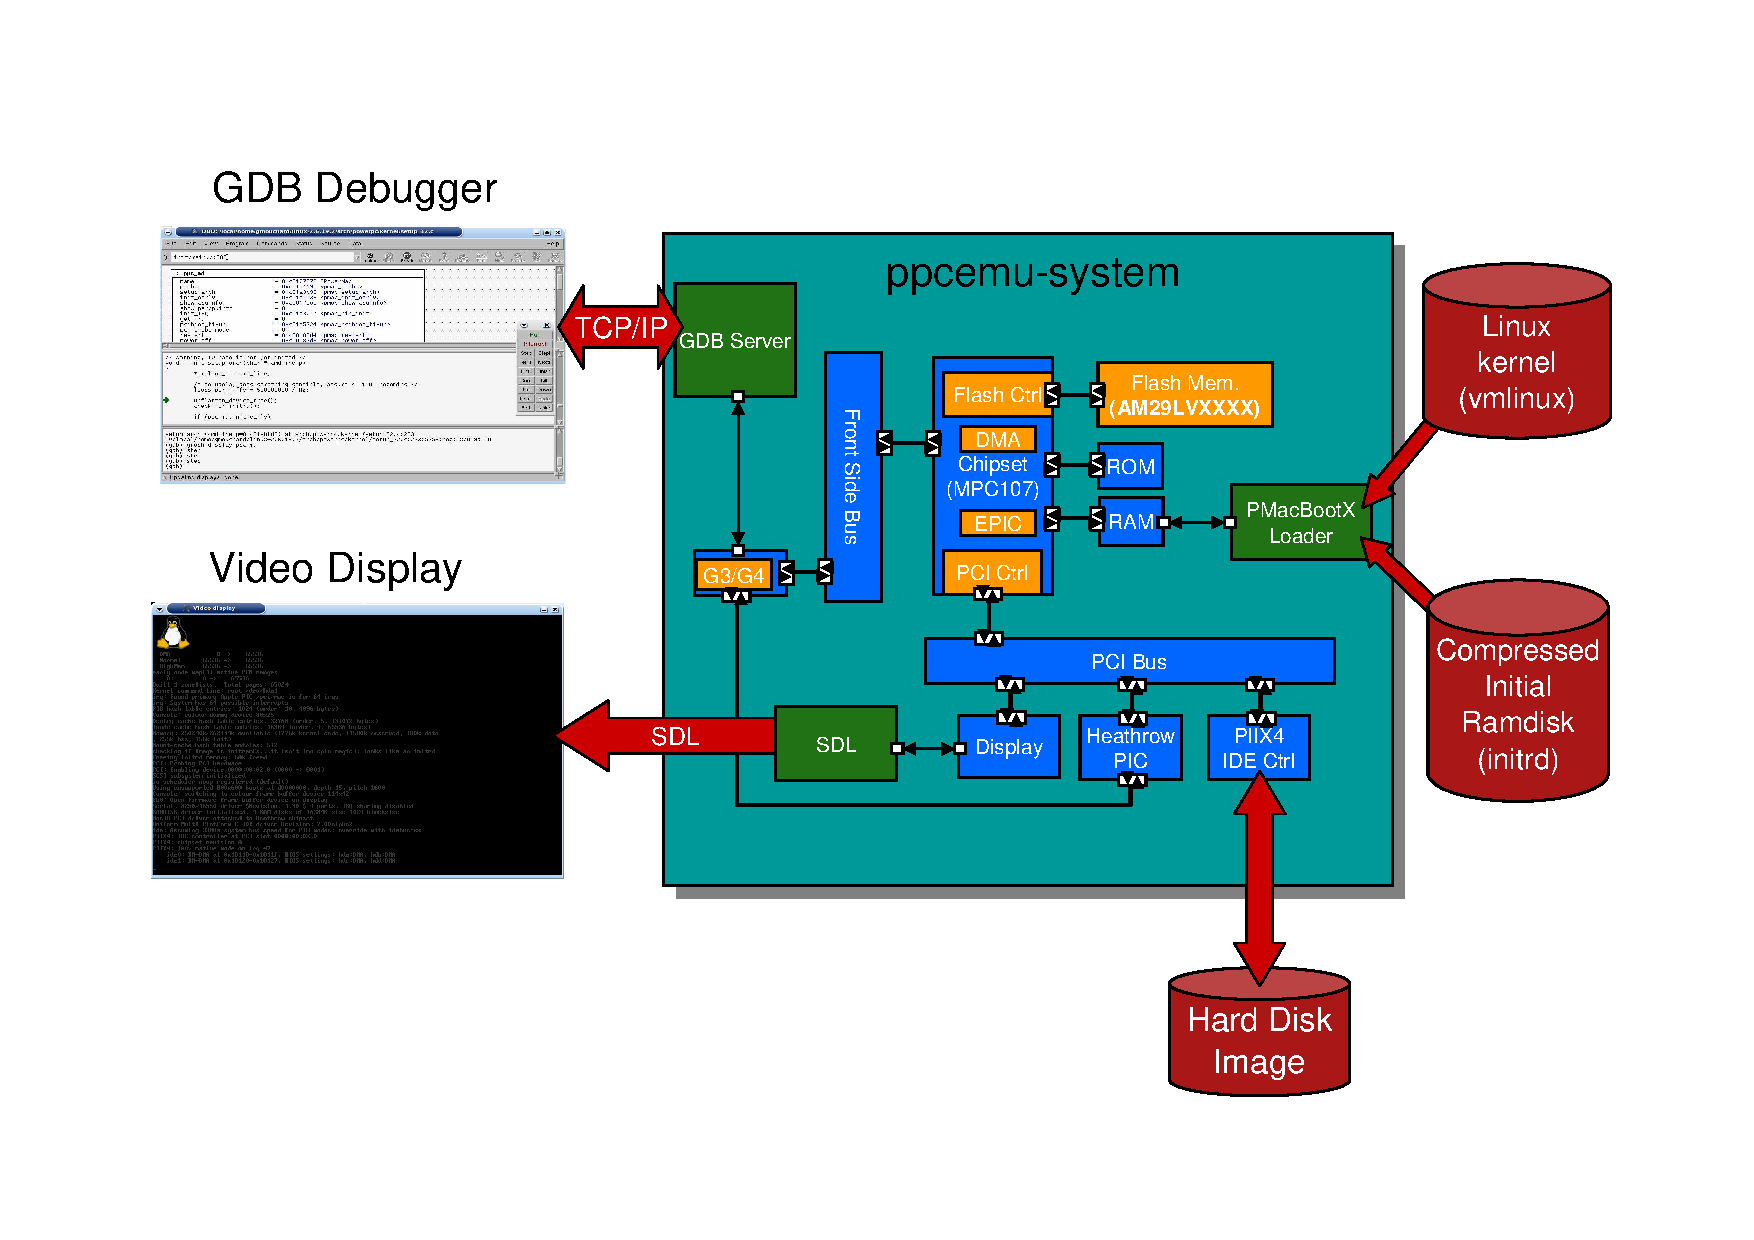
\includegraphics[width=\textwidth]{ppcemu_system/fig_schematic.pdf}
	\end{center}
	\caption{UNISIM ppcemu-system simulator schematic.}
\end{figure}
\noindent The UNISIM ppcemu-system simulator is composed of the following modules and services:
\begin{itemize}\addtolength{\itemsep}{-0.40\baselineskip}
\item \textbf{bus}: Front side bus
\item \textbf{cpu}: PowerPC MPC7447A CPU
\item \textbf{debugger}
\item \textbf{erom}: Memory
\item \textbf{flash}: This module implements an AM29LV800BT flash memory with the following characteristics:\\
Manufacturer ID: 0x010000\\
Device ID word \#0: 0xda2202\\
Size: 4194304 bytes\\
I/O width: 64 bits\\
Number of chips: 4 chips\\
I/O width per chip: 16 bits\\
Size per chip: 1048576 bytes\\
Number of Sectors: 19 sectors\\
8-bit mode support: yes\\
16-bit mode support: yes\\
Access time: 70 ns\\
Byte programming time: 9000 us\\
Word programming time: 110000 us\\
Sector erasing time: 700000000 us\\
Chip erasing time: 14000000000 us\\

\item \textbf{gdb-server}: this service implements the GDB server remote serial protocol over TCP/IP. Standards GDB clients (e.g. gdb, eclipse, ddd) can connect to the simulator to debug the target application that runs within the simulator.
\item \textbf{heathrow}: Heathrow Programmable Interrupt Controller (PIC)
\item \textbf{host-time}: this service is an abstraction layer for the host machine time
\item \textbf{i8042}: i8042 PS/2 keyboard/mouse controller
\item \textbf{inline-debugger}: this service implements a built-in debugger in the terminal console
\item \textbf{memory}: Memory
\item \textbf{mpc107}: MPC107 chipset
\item \textbf{mpc107.DMA}: MPC107 integrated Direct Memory Access (DMA) controller
\item \textbf{mpc107.address\_mapper}: MPC107 Address mapper
\item \textbf{mpc107.atu}: MPC107 integrated Address Translation Unit (ATU)
\item \textbf{mpc107.epic}: MPC107 integrated Embedded Programmable Interrupt Controller (EPIC)
\item \textbf{mpc107.pci\_controller}: MPC107 integrated PCI bus controller
\item \textbf{pci-bus}: PCI bus
\item \textbf{pci-display}: PCI Video frame buffer display
\item \textbf{pci-ide}: PIIX4 IDE controller
\item \textbf{pci-isa-bridge}: PCI-to-ISA bridge
\item \textbf{pmac-linux-kernel-loader}: PowerMac Linux kernel loader
\item \textbf{pmac-linux-kernel-loader.elf32-loader}: this service implements an ELF32 Loader
\item \textbf{pmac-linux-kernel-loader.pmac-bootx}: This service is a PowerMac BootX loader emulator. It allows bootloading a PowerMac Linux kernel with its initial ramdisk and device tree
\item \textbf{profiler}
\item \textbf{sdl}: SDL (Simple DirectMedia Layer) wrapper
\item \textbf{tee-memory-access-reporting}
\item \textbf{tee-memory-access-reporting.tee-memory-access-reporting.control\_selector[0]}
\item \textbf{tee-memory-access-reporting.tee-memory-access-reporting.control\_selector[10]}
\item \textbf{tee-memory-access-reporting.tee-memory-access-reporting.control\_selector[11]}
\item \textbf{tee-memory-access-reporting.tee-memory-access-reporting.control\_selector[12]}
\item \textbf{tee-memory-access-reporting.tee-memory-access-reporting.control\_selector[13]}
\item \textbf{tee-memory-access-reporting.tee-memory-access-reporting.control\_selector[14]}
\item \textbf{tee-memory-access-reporting.tee-memory-access-reporting.control\_selector[15]}
\item \textbf{tee-memory-access-reporting.tee-memory-access-reporting.control\_selector[1]}
\item \textbf{tee-memory-access-reporting.tee-memory-access-reporting.control\_selector[2]}
\item \textbf{tee-memory-access-reporting.tee-memory-access-reporting.control\_selector[3]}
\item \textbf{tee-memory-access-reporting.tee-memory-access-reporting.control\_selector[4]}
\item \textbf{tee-memory-access-reporting.tee-memory-access-reporting.control\_selector[5]}
\item \textbf{tee-memory-access-reporting.tee-memory-access-reporting.control\_selector[6]}
\item \textbf{tee-memory-access-reporting.tee-memory-access-reporting.control\_selector[7]}
\item \textbf{tee-memory-access-reporting.tee-memory-access-reporting.control\_selector[8]}
\item \textbf{tee-memory-access-reporting.tee-memory-access-reporting.control\_selector[9]}
\item \textbf{time}: this service is an abstraction layer for the SystemC kernel time
\end{itemize}
\subsection{Using the UNISIM ppcemu-system simulator}
\label{UNISIM ppcemu-system_using}
The UNISIM ppcemu-system simulator has the following command line options:\\
~\\
\noindent Usage: \texttt{unisim-ppcemu-system-1.0beta5 [<options>] [...]}

\noindent Options:
\begin{itemize}
\item \texttt{--set $<$param=value$>$ or -s $<$param=value$>$}: set value of parameter 'param' to 'value'
\item \texttt{--config $<$XML file$>$ or -c $<$XML file$>$}: configures the simulator with the given XML configuration file
\item \texttt{--get-config $<$XML file$>$ or -g $<$XML file$>$}: get the simulator configuration XML file (you can use it to create your own configuration. This option can be combined with -c to get a new configuration file with existing variables from another file
\item \texttt{--list or -l}: lists all available parameters, their type, and their current value
\item \texttt{--warn or -w}: enable printing of kernel warnings
\item \texttt{--doc $<$Latex file$>$ or -d $<$Latex file$>$}: enable printing a latex documentation
\item \texttt{--version or -v}: displays the program version information
\item \texttt{--share-path $<$path$>$ or -p $<$path$>$}: the path that should be used for the share directory (absolute path)
\item \texttt{--help or -h}: displays this help
\end{itemize}
\subsection{Configuration}
\label{UNISIM ppcemu-system_configuration}
Simulator configuration (see below) can be modified using command line Options \texttt{--set $<$param=value$>$} or \texttt{--config $<$config file$>$}.\\
~\\
\tablehead{\hline}
\tabletail{\hline}
\begin{supertabular}{|p{7.5cm}|p{7.5cm}|}
\multicolumn{2}{|l|}{\textbf{\Large Global}}\\
\hline
\multicolumn{1}{|p{7.5cm}}{\textbf{Name:} \texttt{enable-gdb-server}} & \multicolumn{1}{p{7.5cm}|}{\textbf{Type:} \texttt{parameter}}\\
\multicolumn{1}{|p{7.5cm}}{\textbf{Default:} \texttt{true}} & \multicolumn{1}{p{7.5cm}|}{\textbf{Data type:} \texttt{boolean}}\\
\multicolumn{2}{|p{15cm}|}{\textbf{Valid:} \texttt{true},~\texttt{false}}\\
\multicolumn{2}{|l|}{}\\
\multicolumn{2}{|p{15cm}|}{\textbf{Description:} \newline Enable/Disable GDB server instantiation.}\\
\hline
\multicolumn{1}{|p{7.5cm}}{\textbf{Name:} \texttt{enable-inline-debugger}} & \multicolumn{1}{p{7.5cm}|}{\textbf{Type:} \texttt{parameter}}\\
\multicolumn{1}{|p{7.5cm}}{\textbf{Default:} \texttt{true}} & \multicolumn{1}{p{7.5cm}|}{\textbf{Data type:} \texttt{boolean}}\\
\multicolumn{2}{|p{15cm}|}{\textbf{Valid:} \texttt{true},~\texttt{false}}\\
\multicolumn{2}{|l|}{}\\
\multicolumn{2}{|p{15cm}|}{\textbf{Description:} \newline Enable/Disable inline debugger instantiation.}\\
\hline
\multicolumn{1}{|p{7.5cm}}{\textbf{Name:} \texttt{enable-press-enter-at-exit}} & \multicolumn{1}{p{7.5cm}|}{\textbf{Type:} \texttt{parameter}}\\
\multicolumn{1}{|p{7.5cm}}{\textbf{Default:} \texttt{false}} & \multicolumn{1}{p{7.5cm}|}{\textbf{Data type:} \texttt{boolean}}\\
\multicolumn{2}{|p{15cm}|}{\textbf{Valid:} \texttt{true},~\texttt{false}}\\
\multicolumn{2}{|l|}{}\\
\multicolumn{2}{|p{15cm}|}{\textbf{Description:} \newline Enable/Disable pressing key enter at exit.}\\
\hline
\multicolumn{1}{|p{7.5cm}}{\textbf{Name:} \texttt{estimate-power}} & \multicolumn{1}{p{7.5cm}|}{\textbf{Type:} \texttt{parameter}}\\
\multicolumn{1}{|p{7.5cm}}{\textbf{Default:} \texttt{false}} & \multicolumn{1}{p{7.5cm}|}{\textbf{Data type:} \texttt{boolean}}\\
\multicolumn{2}{|p{15cm}|}{\textbf{Valid:} \texttt{true},~\texttt{false}}\\
\multicolumn{2}{|l|}{}\\
\multicolumn{2}{|p{15cm}|}{\textbf{Description:} \newline Enable/Disable power estimators instantiation.}\\
\hline
\multicolumn{1}{|p{7.5cm}}{\textbf{Name:} \texttt{kernel\_logger.file}} & \multicolumn{1}{p{7.5cm}|}{\textbf{Type:} \texttt{parameter}}\\
\multicolumn{1}{|p{7.5cm}}{\textbf{Default:} \texttt{false}} & \multicolumn{1}{p{7.5cm}|}{\textbf{Data type:} \texttt{boolean}}\\
\multicolumn{2}{|p{15cm}|}{\textbf{Valid:} \texttt{true},~\texttt{false}}\\
\multicolumn{2}{|l|}{}\\
\multicolumn{2}{|p{15cm}|}{\textbf{Description:} \newline Keep logger output in a file.}\\
\hline
\multicolumn{1}{|p{7.5cm}}{\textbf{Name:} \texttt{kernel\_logger.filename}} & \multicolumn{1}{p{7.5cm}|}{\textbf{Type:} \texttt{parameter}}\\
\multicolumn{1}{|p{7.5cm}}{\textbf{Default:} \texttt{logger\_output.txt}} & \multicolumn{1}{p{7.5cm}|}{\textbf{Data type:} \texttt{string}}\\
\multicolumn{2}{|l|}{}\\
\multicolumn{2}{|l|}{}\\
\multicolumn{2}{|p{15cm}|}{\textbf{Description:} \newline Filename to keep logger output \_(the option file must be activated).}\\
\hline
\multicolumn{1}{|p{7.5cm}}{\textbf{Name:} \texttt{kernel\_logger.std\_err}} & \multicolumn{1}{p{7.5cm}|}{\textbf{Type:} \texttt{parameter}}\\
\multicolumn{1}{|p{7.5cm}}{\textbf{Default:} \texttt{true}} & \multicolumn{1}{p{7.5cm}|}{\textbf{Data type:} \texttt{boolean}}\\
\multicolumn{2}{|p{15cm}|}{\textbf{Valid:} \texttt{true},~\texttt{false}}\\
\multicolumn{2}{|l|}{}\\
\multicolumn{2}{|p{15cm}|}{\textbf{Description:} \newline Show logger output through the standard error output.}\\
\hline
\multicolumn{1}{|p{7.5cm}}{\textbf{Name:} \texttt{kernel\_logger.std\_err\_color}} & \multicolumn{1}{p{7.5cm}|}{\textbf{Type:} \texttt{parameter}}\\
\multicolumn{1}{|p{7.5cm}}{\textbf{Default:} \texttt{false}} & \multicolumn{1}{p{7.5cm}|}{\textbf{Data type:} \texttt{boolean}}\\
\multicolumn{2}{|p{15cm}|}{\textbf{Valid:} \texttt{true},~\texttt{false}}\\
\multicolumn{2}{|l|}{}\\
\multicolumn{2}{|p{15cm}|}{\textbf{Description:} \newline Colorize logger output through the standard error output \_(only works if std\_err is active).}\\
\hline
\multicolumn{1}{|p{7.5cm}}{\textbf{Name:} \texttt{kernel\_logger.std\_out}} & \multicolumn{1}{p{7.5cm}|}{\textbf{Type:} \texttt{parameter}}\\
\multicolumn{1}{|p{7.5cm}}{\textbf{Default:} \texttt{false}} & \multicolumn{1}{p{7.5cm}|}{\textbf{Data type:} \texttt{boolean}}\\
\multicolumn{2}{|p{15cm}|}{\textbf{Valid:} \texttt{true},~\texttt{false}}\\
\multicolumn{2}{|l|}{}\\
\multicolumn{2}{|p{15cm}|}{\textbf{Description:} \newline Show logger output through the standard output.}\\
\hline
\multicolumn{1}{|p{7.5cm}}{\textbf{Name:} \texttt{kernel\_logger.std\_out\_color}} & \multicolumn{1}{p{7.5cm}|}{\textbf{Type:} \texttt{parameter}}\\
\multicolumn{1}{|p{7.5cm}}{\textbf{Default:} \texttt{false}} & \multicolumn{1}{p{7.5cm}|}{\textbf{Data type:} \texttt{boolean}}\\
\multicolumn{2}{|p{15cm}|}{\textbf{Valid:} \texttt{true},~\texttt{false}}\\
\multicolumn{2}{|l|}{}\\
\multicolumn{2}{|p{15cm}|}{\textbf{Description:} \newline Colorize logger output through the standard output \_(only works if std\_out is active).}\\
\hline
\multicolumn{1}{|p{7.5cm}}{\textbf{Name:} \texttt{kernel\_logger.xml\_file}} & \multicolumn{1}{p{7.5cm}|}{\textbf{Type:} \texttt{parameter}}\\
\multicolumn{1}{|p{7.5cm}}{\textbf{Default:} \texttt{false}} & \multicolumn{1}{p{7.5cm}|}{\textbf{Data type:} \texttt{boolean}}\\
\multicolumn{2}{|p{15cm}|}{\textbf{Valid:} \texttt{true},~\texttt{false}}\\
\multicolumn{2}{|l|}{}\\
\multicolumn{2}{|p{15cm}|}{\textbf{Description:} \newline Keep logger output in a file xml formatted.}\\
\hline
\multicolumn{1}{|p{7.5cm}}{\textbf{Name:} \texttt{kernel\_logger.xml\_file\_gzipped}} & \multicolumn{1}{p{7.5cm}|}{\textbf{Type:} \texttt{parameter}}\\
\multicolumn{1}{|p{7.5cm}}{\textbf{Default:} \texttt{false}} & \multicolumn{1}{p{7.5cm}|}{\textbf{Data type:} \texttt{boolean}}\\
\multicolumn{2}{|p{15cm}|}{\textbf{Valid:} \texttt{true},~\texttt{false}}\\
\multicolumn{2}{|l|}{}\\
\multicolumn{2}{|p{15cm}|}{\textbf{Description:} \newline If the xml\_file option is active, the output file will be compressed (a .gz extension will be automatically added to the xml\_filename option.}\\
\hline
\multicolumn{1}{|p{7.5cm}}{\textbf{Name:} \texttt{kernel\_logger.xml\_filename}} & \multicolumn{1}{p{7.5cm}|}{\textbf{Type:} \texttt{parameter}}\\
\multicolumn{1}{|p{7.5cm}}{\textbf{Default:} \texttt{logger\_output.xml}} & \multicolumn{1}{p{7.5cm}|}{\textbf{Data type:} \texttt{string}}\\
\multicolumn{2}{|l|}{}\\
\multicolumn{2}{|l|}{}\\
\multicolumn{2}{|p{15cm}|}{\textbf{Description:} \newline Filename to keep logger xml output \_(the option xml\_file must be activated).}\\
\hline
\multicolumn{1}{|p{7.5cm}}{\textbf{Name:} \texttt{message-spy}} & \multicolumn{1}{p{7.5cm}|}{\textbf{Type:} \texttt{parameter}}\\
\multicolumn{1}{|p{7.5cm}}{\textbf{Default:} \texttt{false}} & \multicolumn{1}{p{7.5cm}|}{\textbf{Data type:} \texttt{boolean}}\\
\multicolumn{2}{|p{15cm}|}{\textbf{Valid:} \texttt{true},~\texttt{false}}\\
\multicolumn{2}{|l|}{}\\
\multicolumn{2}{|p{15cm}|}{\textbf{Description:} \newline Enable/Disable message spies instantiation.}\\
\hline
\hline
\multicolumn{2}{|l|}{\textbf{\Large bus}}\\
\hline
\multicolumn{1}{|p{7.5cm}}{\textbf{Name:} \texttt{bus.verbose}} & \multicolumn{1}{p{7.5cm}|}{\textbf{Type:} \texttt{parameter}}\\
\multicolumn{1}{|p{7.5cm}}{\textbf{Default:} \texttt{false}} & \multicolumn{1}{p{7.5cm}|}{\textbf{Data type:} \texttt{boolean}}\\
\multicolumn{2}{|p{15cm}|}{\textbf{Valid:} \texttt{true},~\texttt{false}}\\
\multicolumn{2}{|l|}{}\\
\multicolumn{2}{|p{15cm}|}{\textbf{Description:} \newline enable/disable verbosity.}\\
\hline
\multicolumn{1}{|p{7.5cm}}{\textbf{Name:} \texttt{bus.cycle-time}} & \multicolumn{1}{p{7.5cm}|}{\textbf{Type:} \texttt{parameter}}\\
\multicolumn{1}{|p{7.5cm}}{\textbf{Default:} \texttt{13333 ps}} & \multicolumn{1}{p{7.5cm}|}{\textbf{Data type:} \texttt{sc\_time}}\\
\multicolumn{2}{|l|}{}\\
\multicolumn{2}{|l|}{}\\
\multicolumn{2}{|p{15cm}|}{\textbf{Description:} \newline cycle time.}\\
\hline
\hline
\multicolumn{2}{|l|}{\textbf{\Large cpu}}\\
\hline
\multicolumn{1}{|p{7.5cm}}{\textbf{Name:} \texttt{cpu.cpu-cycle-time}} & \multicolumn{1}{p{7.5cm}|}{\textbf{Type:} \texttt{parameter}}\\
\multicolumn{1}{|p{7.5cm}}{\textbf{Default:} \texttt{3333}} & \multicolumn{1}{p{7.5cm}|}{\textbf{Data type:} \texttt{unsigned 64-bit integer}}\\
\multicolumn{2}{|l|}{}\\
\multicolumn{2}{|l|}{}\\
\multicolumn{2}{|p{15cm}|}{\textbf{Description:} \newline CPU cycle time in picoseconds.}\\
\hline
\multicolumn{1}{|p{7.5cm}}{\textbf{Name:} \texttt{cpu.voltage}} & \multicolumn{1}{p{7.5cm}|}{\textbf{Type:} \texttt{parameter}}\\
\multicolumn{1}{|p{7.5cm}}{\textbf{Default:} \texttt{1300}} & \multicolumn{1}{p{7.5cm}|}{\textbf{Data type:} \texttt{unsigned 64-bit integer}}\\
\multicolumn{2}{|l|}{}\\
\multicolumn{2}{|l|}{}\\
\multicolumn{2}{|p{15cm}|}{\textbf{Description:} \newline CPU voltage in mV.}\\
\hline
\multicolumn{1}{|p{7.5cm}}{\textbf{Name:} \texttt{cpu.max-inst}} & \multicolumn{1}{p{7.5cm}|}{\textbf{Type:} \texttt{parameter}}\\
\multicolumn{1}{|p{7.5cm}}{\textbf{Default:} \texttt{18446744073709551615}} & \multicolumn{1}{p{7.5cm}|}{\textbf{Data type:} \texttt{unsigned 64-bit integer}}\\
\multicolumn{2}{|l|}{}\\
\multicolumn{2}{|l|}{}\\
\multicolumn{2}{|p{15cm}|}{\textbf{Description:} \newline maximum number of instructions to simulate.}\\
\hline
\multicolumn{1}{|p{7.5cm}}{\textbf{Name:} \texttt{cpu.verbose-all}} & \multicolumn{1}{p{7.5cm}|}{\textbf{Type:} \texttt{parameter}}\\
\multicolumn{1}{|p{7.5cm}}{\textbf{Default:} \texttt{false}} & \multicolumn{1}{p{7.5cm}|}{\textbf{Data type:} \texttt{boolean}}\\
\multicolumn{2}{|p{15cm}|}{\textbf{Valid:} \texttt{true},~\texttt{false}}\\
\multicolumn{2}{|l|}{}\\
\multicolumn{2}{|p{15cm}|}{\textbf{Description:} \newline globally enable/disable verbosity.}\\
\hline
\multicolumn{1}{|p{7.5cm}}{\textbf{Name:} \texttt{cpu.verbose-setup}} & \multicolumn{1}{p{7.5cm}|}{\textbf{Type:} \texttt{parameter}}\\
\multicolumn{1}{|p{7.5cm}}{\textbf{Default:} \texttt{false}} & \multicolumn{1}{p{7.5cm}|}{\textbf{Data type:} \texttt{boolean}}\\
\multicolumn{2}{|p{15cm}|}{\textbf{Valid:} \texttt{true},~\texttt{false}}\\
\multicolumn{2}{|l|}{}\\
\multicolumn{2}{|p{15cm}|}{\textbf{Description:} \newline enable/disable verbosity while setup.}\\
\hline
\multicolumn{1}{|p{7.5cm}}{\textbf{Name:} \texttt{cpu.verbose-step}} & \multicolumn{1}{p{7.5cm}|}{\textbf{Type:} \texttt{parameter}}\\
\multicolumn{1}{|p{7.5cm}}{\textbf{Default:} \texttt{false}} & \multicolumn{1}{p{7.5cm}|}{\textbf{Data type:} \texttt{boolean}}\\
\multicolumn{2}{|p{15cm}|}{\textbf{Valid:} \texttt{true},~\texttt{false}}\\
\multicolumn{2}{|l|}{}\\
\multicolumn{2}{|p{15cm}|}{\textbf{Description:} \newline enable/disable verbosity when simulating an instruction.}\\
\hline
\multicolumn{1}{|p{7.5cm}}{\textbf{Name:} \texttt{cpu.verbose-dtlb}} & \multicolumn{1}{p{7.5cm}|}{\textbf{Type:} \texttt{parameter}}\\
\multicolumn{1}{|p{7.5cm}}{\textbf{Default:} \texttt{false}} & \multicolumn{1}{p{7.5cm}|}{\textbf{Data type:} \texttt{boolean}}\\
\multicolumn{2}{|p{15cm}|}{\textbf{Valid:} \texttt{true},~\texttt{false}}\\
\multicolumn{2}{|l|}{}\\
\multicolumn{2}{|p{15cm}|}{\textbf{Description:} \newline enable/disable verbosity when accessing data translation lookahead buffer.}\\
\hline
\multicolumn{1}{|p{7.5cm}}{\textbf{Name:} \texttt{cpu.verbose-itlb}} & \multicolumn{1}{p{7.5cm}|}{\textbf{Type:} \texttt{parameter}}\\
\multicolumn{1}{|p{7.5cm}}{\textbf{Default:} \texttt{false}} & \multicolumn{1}{p{7.5cm}|}{\textbf{Data type:} \texttt{boolean}}\\
\multicolumn{2}{|p{15cm}|}{\textbf{Valid:} \texttt{true},~\texttt{false}}\\
\multicolumn{2}{|l|}{}\\
\multicolumn{2}{|p{15cm}|}{\textbf{Description:} \newline enable/disable verbosity when accessing instruction translation lookahead buffer.}\\
\hline
\multicolumn{1}{|p{7.5cm}}{\textbf{Name:} \texttt{cpu.verbose-dl1}} & \multicolumn{1}{p{7.5cm}|}{\textbf{Type:} \texttt{parameter}}\\
\multicolumn{1}{|p{7.5cm}}{\textbf{Default:} \texttt{false}} & \multicolumn{1}{p{7.5cm}|}{\textbf{Data type:} \texttt{boolean}}\\
\multicolumn{2}{|p{15cm}|}{\textbf{Valid:} \texttt{true},~\texttt{false}}\\
\multicolumn{2}{|l|}{}\\
\multicolumn{2}{|p{15cm}|}{\textbf{Description:} \newline enable/disable verbosity when accessing L1 data cache.}\\
\hline
\multicolumn{1}{|p{7.5cm}}{\textbf{Name:} \texttt{cpu.verbose-il1}} & \multicolumn{1}{p{7.5cm}|}{\textbf{Type:} \texttt{parameter}}\\
\multicolumn{1}{|p{7.5cm}}{\textbf{Default:} \texttt{false}} & \multicolumn{1}{p{7.5cm}|}{\textbf{Data type:} \texttt{boolean}}\\
\multicolumn{2}{|p{15cm}|}{\textbf{Valid:} \texttt{true},~\texttt{false}}\\
\multicolumn{2}{|l|}{}\\
\multicolumn{2}{|p{15cm}|}{\textbf{Description:} \newline enable/disable verbosity when accessing L1 instruction cache.}\\
\hline
\multicolumn{1}{|p{7.5cm}}{\textbf{Name:} \texttt{cpu.verbose-l2}} & \multicolumn{1}{p{7.5cm}|}{\textbf{Type:} \texttt{parameter}}\\
\multicolumn{1}{|p{7.5cm}}{\textbf{Default:} \texttt{false}} & \multicolumn{1}{p{7.5cm}|}{\textbf{Data type:} \texttt{boolean}}\\
\multicolumn{2}{|p{15cm}|}{\textbf{Valid:} \texttt{true},~\texttt{false}}\\
\multicolumn{2}{|l|}{}\\
\multicolumn{2}{|p{15cm}|}{\textbf{Description:} \newline enable/disable verbosity when accessing L2 unified cache.}\\
\hline
\multicolumn{1}{|p{7.5cm}}{\textbf{Name:} \texttt{cpu.verbose-load}} & \multicolumn{1}{p{7.5cm}|}{\textbf{Type:} \texttt{parameter}}\\
\multicolumn{1}{|p{7.5cm}}{\textbf{Default:} \texttt{false}} & \multicolumn{1}{p{7.5cm}|}{\textbf{Data type:} \texttt{boolean}}\\
\multicolumn{2}{|p{15cm}|}{\textbf{Valid:} \texttt{true},~\texttt{false}}\\
\multicolumn{2}{|l|}{}\\
\multicolumn{2}{|p{15cm}|}{\textbf{Description:} \newline enable/disable verbosity when simulating a load.}\\
\hline
\multicolumn{1}{|p{7.5cm}}{\textbf{Name:} \texttt{cpu.verbose-store}} & \multicolumn{1}{p{7.5cm}|}{\textbf{Type:} \texttt{parameter}}\\
\multicolumn{1}{|p{7.5cm}}{\textbf{Default:} \texttt{false}} & \multicolumn{1}{p{7.5cm}|}{\textbf{Data type:} \texttt{boolean}}\\
\multicolumn{2}{|p{15cm}|}{\textbf{Valid:} \texttt{true},~\texttt{false}}\\
\multicolumn{2}{|l|}{}\\
\multicolumn{2}{|p{15cm}|}{\textbf{Description:} \newline enable/disable verbosity when simulating a store.}\\
\hline
\multicolumn{1}{|p{7.5cm}}{\textbf{Name:} \texttt{cpu.verbose-read-memory}} & \multicolumn{1}{p{7.5cm}|}{\textbf{Type:} \texttt{parameter}}\\
\multicolumn{1}{|p{7.5cm}}{\textbf{Default:} \texttt{false}} & \multicolumn{1}{p{7.5cm}|}{\textbf{Data type:} \texttt{boolean}}\\
\multicolumn{2}{|p{15cm}|}{\textbf{Valid:} \texttt{true},~\texttt{false}}\\
\multicolumn{2}{|l|}{}\\
\multicolumn{2}{|p{15cm}|}{\textbf{Description:} \newline enable/disable verbosity when reading memory for a debug purpose.}\\
\hline
\multicolumn{1}{|p{7.5cm}}{\textbf{Name:} \texttt{cpu.verbose-write-memory}} & \multicolumn{1}{p{7.5cm}|}{\textbf{Type:} \texttt{parameter}}\\
\multicolumn{1}{|p{7.5cm}}{\textbf{Default:} \texttt{false}} & \multicolumn{1}{p{7.5cm}|}{\textbf{Data type:} \texttt{boolean}}\\
\multicolumn{2}{|p{15cm}|}{\textbf{Valid:} \texttt{true},~\texttt{false}}\\
\multicolumn{2}{|l|}{}\\
\multicolumn{2}{|p{15cm}|}{\textbf{Description:} \newline enable/disable verbosity when writing memory for a debug purpose.}\\
\hline
\multicolumn{1}{|p{7.5cm}}{\textbf{Name:} \texttt{cpu.verbose-exception}} & \multicolumn{1}{p{7.5cm}|}{\textbf{Type:} \texttt{parameter}}\\
\multicolumn{1}{|p{7.5cm}}{\textbf{Default:} \texttt{false}} & \multicolumn{1}{p{7.5cm}|}{\textbf{Data type:} \texttt{boolean}}\\
\multicolumn{2}{|p{15cm}|}{\textbf{Valid:} \texttt{true},~\texttt{false}}\\
\multicolumn{2}{|l|}{}\\
\multicolumn{2}{|p{15cm}|}{\textbf{Description:} \newline enable/disable verbosity when handling exceptions.}\\
\hline
\multicolumn{1}{|p{7.5cm}}{\textbf{Name:} \texttt{cpu.verbose-set-msr}} & \multicolumn{1}{p{7.5cm}|}{\textbf{Type:} \texttt{parameter}}\\
\multicolumn{1}{|p{7.5cm}}{\textbf{Default:} \texttt{false}} & \multicolumn{1}{p{7.5cm}|}{\textbf{Data type:} \texttt{boolean}}\\
\multicolumn{2}{|p{15cm}|}{\textbf{Valid:} \texttt{true},~\texttt{false}}\\
\multicolumn{2}{|l|}{}\\
\multicolumn{2}{|p{15cm}|}{\textbf{Description:} \newline enable/disable verbosity when setting MSR.}\\
\hline
\multicolumn{1}{|p{7.5cm}}{\textbf{Name:} \texttt{cpu.verbose-set-hid0}} & \multicolumn{1}{p{7.5cm}|}{\textbf{Type:} \texttt{parameter}}\\
\multicolumn{1}{|p{7.5cm}}{\textbf{Default:} \texttt{false}} & \multicolumn{1}{p{7.5cm}|}{\textbf{Data type:} \texttt{boolean}}\\
\multicolumn{2}{|p{15cm}|}{\textbf{Valid:} \texttt{true},~\texttt{false}}\\
\multicolumn{2}{|l|}{}\\
\multicolumn{2}{|p{15cm}|}{\textbf{Description:} \newline enable/disable verbosity when setting HID0.}\\
\hline
\multicolumn{1}{|p{7.5cm}}{\textbf{Name:} \texttt{cpu.verbose-set-hid1}} & \multicolumn{1}{p{7.5cm}|}{\textbf{Type:} \texttt{parameter}}\\
\multicolumn{1}{|p{7.5cm}}{\textbf{Default:} \texttt{false}} & \multicolumn{1}{p{7.5cm}|}{\textbf{Data type:} \texttt{boolean}}\\
\multicolumn{2}{|p{15cm}|}{\textbf{Valid:} \texttt{true},~\texttt{false}}\\
\multicolumn{2}{|l|}{}\\
\multicolumn{2}{|p{15cm}|}{\textbf{Description:} \newline enable/disable verbosity when setting HID1.}\\
\hline
\multicolumn{1}{|p{7.5cm}}{\textbf{Name:} \texttt{cpu.verbose-set-hid2}} & \multicolumn{1}{p{7.5cm}|}{\textbf{Type:} \texttt{parameter}}\\
\multicolumn{1}{|p{7.5cm}}{\textbf{Default:} \texttt{false}} & \multicolumn{1}{p{7.5cm}|}{\textbf{Data type:} \texttt{boolean}}\\
\multicolumn{2}{|p{15cm}|}{\textbf{Valid:} \texttt{true},~\texttt{false}}\\
\multicolumn{2}{|l|}{}\\
\multicolumn{2}{|p{15cm}|}{\textbf{Description:} \newline enable/disable verbosity when setting HID2.}\\
\hline
\multicolumn{1}{|p{7.5cm}}{\textbf{Name:} \texttt{cpu.verbose-set-l2cr}} & \multicolumn{1}{p{7.5cm}|}{\textbf{Type:} \texttt{parameter}}\\
\multicolumn{1}{|p{7.5cm}}{\textbf{Default:} \texttt{false}} & \multicolumn{1}{p{7.5cm}|}{\textbf{Data type:} \texttt{boolean}}\\
\multicolumn{2}{|p{15cm}|}{\textbf{Valid:} \texttt{true},~\texttt{false}}\\
\multicolumn{2}{|l|}{}\\
\multicolumn{2}{|p{15cm}|}{\textbf{Description:} \newline enable/disable verbosity when setting L2CR.}\\
\hline
\multicolumn{1}{|p{7.5cm}}{\textbf{Name:} \texttt{cpu.enable-linux-printk-snooping}} & \multicolumn{1}{p{7.5cm}|}{\textbf{Type:} \texttt{parameter}}\\
\multicolumn{1}{|p{7.5cm}}{\textbf{Default:} \texttt{false}} & \multicolumn{1}{p{7.5cm}|}{\textbf{Data type:} \texttt{boolean}}\\
\multicolumn{2}{|p{15cm}|}{\textbf{Valid:} \texttt{true},~\texttt{false}}\\
\multicolumn{2}{|l|}{}\\
\multicolumn{2}{|p{15cm}|}{\textbf{Description:} \newline enable/disable linux printk buffer snooping.}\\
\hline
\multicolumn{1}{|p{7.5cm}}{\textbf{Name:} \texttt{cpu.enable-linux-syscall-snooping}} & \multicolumn{1}{p{7.5cm}|}{\textbf{Type:} \texttt{parameter}}\\
\multicolumn{1}{|p{7.5cm}}{\textbf{Default:} \texttt{false}} & \multicolumn{1}{p{7.5cm}|}{\textbf{Data type:} \texttt{boolean}}\\
\multicolumn{2}{|p{15cm}|}{\textbf{Valid:} \texttt{true},~\texttt{false}}\\
\multicolumn{2}{|l|}{}\\
\multicolumn{2}{|p{15cm}|}{\textbf{Description:} \newline enable/disable linux syscall snooping.}\\
\hline
\multicolumn{1}{|p{7.5cm}}{\textbf{Name:} \texttt{cpu.trap-on-instruction-counter}} & \multicolumn{1}{p{7.5cm}|}{\textbf{Type:} \texttt{parameter}}\\
\multicolumn{1}{|p{7.5cm}}{\textbf{Default:} \texttt{18446744073709551615}} & \multicolumn{1}{p{7.5cm}|}{\textbf{Data type:} \texttt{unsigned 64-bit integer}}\\
\multicolumn{2}{|l|}{}\\
\multicolumn{2}{|l|}{}\\
\multicolumn{2}{|p{15cm}|}{\textbf{Description:} \newline number of simulated instruction before traping.}\\
\hline
\multicolumn{1}{|p{7.5cm}}{\textbf{Name:} \texttt{cpu.halt-on}} & \multicolumn{1}{p{7.5cm}|}{\textbf{Type:} \texttt{parameter}}\\
\multicolumn{1}{|p{7.5cm}}{\textbf{Default:} \texttt{}} & \multicolumn{1}{p{7.5cm}|}{\textbf{Data type:} \texttt{string}}\\
\multicolumn{2}{|l|}{}\\
\multicolumn{2}{|l|}{}\\
\multicolumn{2}{|p{15cm}|}{\textbf{Description:} \newline Symbol or address where to stop simulation.}\\
\hline
\multicolumn{1}{|p{7.5cm}}{\textbf{Name:} \texttt{cpu.bus-cycle-time}} & \multicolumn{1}{p{7.5cm}|}{\textbf{Type:} \texttt{parameter}}\\
\multicolumn{1}{|p{7.5cm}}{\textbf{Default:} \texttt{13333 ps}} & \multicolumn{1}{p{7.5cm}|}{\textbf{Data type:} \texttt{sc\_time}}\\
\multicolumn{2}{|l|}{}\\
\multicolumn{2}{|l|}{}\\
\multicolumn{2}{|p{15cm}|}{\textbf{Description:} \newline bus cycle time.}\\
\hline
\multicolumn{1}{|p{7.5cm}}{\textbf{Name:} \texttt{cpu.nice-time}} & \multicolumn{1}{p{7.5cm}|}{\textbf{Type:} \texttt{parameter}}\\
\multicolumn{1}{|p{7.5cm}}{\textbf{Default:} \texttt{1 ms}} & \multicolumn{1}{p{7.5cm}|}{\textbf{Data type:} \texttt{sc\_time}}\\
\multicolumn{2}{|l|}{}\\
\multicolumn{2}{|l|}{}\\
\multicolumn{2}{|p{15cm}|}{\textbf{Description:} \newline maximum time between synchonizations.}\\
\hline
\multicolumn{1}{|p{7.5cm}}{\textbf{Name:} \texttt{cpu.ipc}} & \multicolumn{1}{p{7.5cm}|}{\textbf{Type:} \texttt{parameter}}\\
\multicolumn{1}{|p{7.5cm}}{\textbf{Default:} \texttt{1}} & \multicolumn{1}{p{7.5cm}|}{\textbf{Data type:} \texttt{double precision floating-point}}\\
\multicolumn{2}{|l|}{}\\
\multicolumn{2}{|l|}{}\\
\multicolumn{2}{|p{15cm}|}{\textbf{Description:} \newline targeted average instructions per second.}\\
\hline
\multicolumn{1}{|p{7.5cm}}{\textbf{Name:} \texttt{cpu.enable-host-idle}} & \multicolumn{1}{p{7.5cm}|}{\textbf{Type:} \texttt{parameter}}\\
\multicolumn{1}{|p{7.5cm}}{\textbf{Default:} \texttt{false}} & \multicolumn{1}{p{7.5cm}|}{\textbf{Data type:} \texttt{boolean}}\\
\multicolumn{2}{|p{15cm}|}{\textbf{Valid:} \texttt{true},~\texttt{false}}\\
\multicolumn{2}{|l|}{}\\
\multicolumn{2}{|p{15cm}|}{\textbf{Description:} \newline Enable/Disable host idle periods when target is idle.}\\
\hline
\hline
\multicolumn{2}{|l|}{\textbf{\Large debugger}}\\
\hline
\multicolumn{1}{|p{7.5cm}}{\textbf{Name:} \texttt{debugger.verbose}} & \multicolumn{1}{p{7.5cm}|}{\textbf{Type:} \texttt{parameter}}\\
\multicolumn{1}{|p{7.5cm}}{\textbf{Default:} \texttt{false}} & \multicolumn{1}{p{7.5cm}|}{\textbf{Data type:} \texttt{boolean}}\\
\multicolumn{2}{|p{15cm}|}{\textbf{Valid:} \texttt{true},~\texttt{false}}\\
\multicolumn{2}{|l|}{}\\
\multicolumn{2}{|p{15cm}|}{\textbf{Description:} \newline Enable/Disable verbosity.}\\
\hline
\multicolumn{1}{|p{7.5cm}}{\textbf{Name:} \texttt{debugger.dwarf-to-html-output-} \newline$\hookrightarrow$\texttt{directory}} & \multicolumn{1}{p{7.5cm}|}{\textbf{Type:} \texttt{parameter}}\\
\multicolumn{1}{|p{7.5cm}}{\textbf{Default:} \texttt{}} & \multicolumn{1}{p{7.5cm}|}{\textbf{Data type:} \texttt{string}}\\
\multicolumn{2}{|l|}{}\\
\multicolumn{2}{|l|}{}\\
\multicolumn{2}{|p{15cm}|}{\textbf{Description:} \newline DWARF v2/v3 to HTML output directory.}\\
\hline
\multicolumn{1}{|p{7.5cm}}{\textbf{Name:} \texttt{debugger.dwarf-register-number-} \newline$\hookrightarrow$\texttt{mapping-filename}} & \multicolumn{1}{p{7.5cm}|}{\textbf{Type:} \texttt{parameter}}\\
\multicolumn{1}{|p{7.5cm}}{\textbf{Default:} \texttt{powerpc\_eabi\_gcc\_dwarf\_register\_} \newline$\hookrightarrow$\texttt{number\_mapping.xml}} & \multicolumn{1}{p{7.5cm}|}{\textbf{Data type:} \texttt{string}}\\
\multicolumn{2}{|l|}{}\\
\multicolumn{2}{|l|}{}\\
\multicolumn{2}{|p{15cm}|}{\textbf{Description:} \newline DWARF register number mapping filename.}\\
\hline
\multicolumn{1}{|p{7.5cm}}{\textbf{Name:} \texttt{debugger.parse-dwarf}} & \multicolumn{1}{p{7.5cm}|}{\textbf{Type:} \texttt{parameter}}\\
\multicolumn{1}{|p{7.5cm}}{\textbf{Default:} \texttt{true}} & \multicolumn{1}{p{7.5cm}|}{\textbf{Data type:} \texttt{boolean}}\\
\multicolumn{2}{|p{15cm}|}{\textbf{Valid:} \texttt{true},~\texttt{false}}\\
\multicolumn{2}{|l|}{}\\
\multicolumn{2}{|p{15cm}|}{\textbf{Description:} \newline Enable/Disable parsing of DWARF debugging informations.}\\
\hline
\multicolumn{1}{|p{7.5cm}}{\textbf{Name:} \texttt{debugger.debug-dwarf}} & \multicolumn{1}{p{7.5cm}|}{\textbf{Type:} \texttt{parameter}}\\
\multicolumn{1}{|p{7.5cm}}{\textbf{Default:} \texttt{false}} & \multicolumn{1}{p{7.5cm}|}{\textbf{Data type:} \texttt{boolean}}\\
\multicolumn{2}{|p{15cm}|}{\textbf{Valid:} \texttt{true},~\texttt{false}}\\
\multicolumn{2}{|l|}{}\\
\multicolumn{2}{|p{15cm}|}{\textbf{Description:} \newline Enable/Disable debugging of DWARF.}\\
\hline
\hline
\multicolumn{2}{|l|}{\textbf{\Large erom}}\\
\hline
\multicolumn{1}{|p{7.5cm}}{\textbf{Name:} \texttt{erom.org}} & \multicolumn{1}{p{7.5cm}|}{\textbf{Type:} \texttt{parameter}}\\
\multicolumn{1}{|p{7.5cm}}{\textbf{Default:} \texttt{0x78000000}} & \multicolumn{1}{p{7.5cm}|}{\textbf{Data type:} \texttt{unsigned 32-bit integer}}\\
\multicolumn{2}{|l|}{}\\
\multicolumn{2}{|l|}{}\\
\multicolumn{2}{|p{15cm}|}{\textbf{Description:} \newline memory origin/base address.}\\
\hline
\multicolumn{1}{|p{7.5cm}}{\textbf{Name:} \texttt{erom.bytesize}} & \multicolumn{1}{p{7.5cm}|}{\textbf{Type:} \texttt{parameter}}\\
\multicolumn{1}{|p{7.5cm}}{\textbf{Default:} \texttt{16777216}} & \multicolumn{1}{p{7.5cm}|}{\textbf{Data type:} \texttt{unsigned 32-bit integer}}\\
\multicolumn{2}{|l|}{}\\
\multicolumn{2}{|l|}{}\\
\multicolumn{2}{|p{15cm}|}{\textbf{Description:} \newline memory size in bytes.}\\
\hline
\multicolumn{1}{|p{7.5cm}}{\textbf{Name:} \texttt{erom.initial-byte-value}} & \multicolumn{1}{p{7.5cm}|}{\textbf{Type:} \texttt{parameter}}\\
\multicolumn{1}{|p{7.5cm}}{\textbf{Default:} \texttt{0x00}} & \multicolumn{1}{p{7.5cm}|}{\textbf{Data type:} \texttt{unsigned 8-bit integer}}\\
\multicolumn{2}{|l|}{}\\
\hline
\multicolumn{1}{|p{7.5cm}}{\textbf{Name:} \texttt{erom.verbose}} & \multicolumn{1}{p{7.5cm}|}{\textbf{Type:} \texttt{parameter}}\\
\multicolumn{1}{|p{7.5cm}}{\textbf{Default:} \texttt{false}} & \multicolumn{1}{p{7.5cm}|}{\textbf{Data type:} \texttt{boolean}}\\
\multicolumn{2}{|p{15cm}|}{\textbf{Valid:} \texttt{true},~\texttt{false}}\\
\multicolumn{2}{|l|}{}\\
\multicolumn{2}{|p{15cm}|}{\textbf{Description:} \newline enable/disable verbosity.}\\
\hline
\multicolumn{1}{|p{7.5cm}}{\textbf{Name:} \texttt{erom.cycle-time}} & \multicolumn{1}{p{7.5cm}|}{\textbf{Type:} \texttt{parameter}}\\
\multicolumn{1}{|p{7.5cm}}{\textbf{Default:} \texttt{13333 ps}} & \multicolumn{1}{p{7.5cm}|}{\textbf{Data type:} \texttt{sc\_time}}\\
\multicolumn{2}{|l|}{}\\
\multicolumn{2}{|l|}{}\\
\multicolumn{2}{|p{15cm}|}{\textbf{Description:} \newline RAM memory cycle time.}\\
\hline
\hline
\multicolumn{2}{|l|}{\textbf{\Large flash}}\\
\hline
\multicolumn{1}{|p{7.5cm}}{\textbf{Name:} \texttt{flash.verbose}} & \multicolumn{1}{p{7.5cm}|}{\textbf{Type:} \texttt{parameter}}\\
\multicolumn{1}{|p{7.5cm}}{\textbf{Default:} \texttt{false}} & \multicolumn{1}{p{7.5cm}|}{\textbf{Data type:} \texttt{boolean}}\\
\multicolumn{2}{|p{15cm}|}{\textbf{Valid:} \texttt{true},~\texttt{false}}\\
\multicolumn{2}{|l|}{}\\
\multicolumn{2}{|p{15cm}|}{\textbf{Description:} \newline enable/disable verbosity.}\\
\hline
\multicolumn{1}{|p{7.5cm}}{\textbf{Name:} \texttt{flash.org}} & \multicolumn{1}{p{7.5cm}|}{\textbf{Type:} \texttt{parameter}}\\
\multicolumn{1}{|p{7.5cm}}{\textbf{Default:} \texttt{0xff800000}} & \multicolumn{1}{p{7.5cm}|}{\textbf{Data type:} \texttt{unsigned 32-bit integer}}\\
\multicolumn{2}{|l|}{}\\
\multicolumn{2}{|l|}{}\\
\multicolumn{2}{|p{15cm}|}{\textbf{Description:} \newline flash memory base address.}\\
\hline
\multicolumn{1}{|p{7.5cm}}{\textbf{Name:} \texttt{flash.bytesize}} & \multicolumn{1}{p{7.5cm}|}{\textbf{Type:} \texttt{parameter}}\\
\multicolumn{1}{|p{7.5cm}}{\textbf{Default:} \texttt{8388608}} & \multicolumn{1}{p{7.5cm}|}{\textbf{Data type:} \texttt{unsigned 32-bit integer}}\\
\multicolumn{2}{|l|}{}\\
\multicolumn{2}{|l|}{}\\
\multicolumn{2}{|p{15cm}|}{\textbf{Description:} \newline flash memory size in bytes.}\\
\hline
\multicolumn{1}{|p{7.5cm}}{\textbf{Name:} \texttt{flash.endian}} & \multicolumn{1}{p{7.5cm}|}{\textbf{Type:} \texttt{parameter}}\\
\multicolumn{1}{|p{7.5cm}}{\textbf{Default:} \texttt{big-endian}} & \multicolumn{1}{p{7.5cm}|}{\textbf{Data type:} \texttt{endianess}}\\
\multicolumn{2}{|p{15cm}|}{\textbf{Valid:} \texttt{little-endian},~\texttt{big-endian}}\\
\multicolumn{2}{|l|}{}\\
\multicolumn{2}{|p{15cm}|}{\textbf{Description:} \newline endianness of flash memory.}\\
\hline
\multicolumn{1}{|p{7.5cm}}{\textbf{Name:} \texttt{flash.sector-protect[0]}} & \multicolumn{1}{p{7.5cm}|}{\textbf{Type:} \texttt{parameter}}\\
\multicolumn{1}{|p{7.5cm}}{\textbf{Default:} \texttt{false}} & \multicolumn{1}{p{7.5cm}|}{\textbf{Data type:} \texttt{boolean}}\\
\multicolumn{2}{|p{15cm}|}{\textbf{Valid:} \texttt{true},~\texttt{false}}\\
\multicolumn{2}{|l|}{}\\
\multicolumn{2}{|p{15cm}|}{\textbf{Description:} \newline enable/disable sector write protection.}\\
\hline
\multicolumn{1}{|p{7.5cm}}{\textbf{Name:} \texttt{flash.sector-protect[1]}} & \multicolumn{1}{p{7.5cm}|}{\textbf{Type:} \texttt{parameter}}\\
\multicolumn{1}{|p{7.5cm}}{\textbf{Default:} \texttt{false}} & \multicolumn{1}{p{7.5cm}|}{\textbf{Data type:} \texttt{boolean}}\\
\multicolumn{2}{|p{15cm}|}{\textbf{Valid:} \texttt{true},~\texttt{false}}\\
\multicolumn{2}{|l|}{}\\
\multicolumn{2}{|p{15cm}|}{\textbf{Description:} \newline enable/disable sector write protection.}\\
\hline
\multicolumn{1}{|p{7.5cm}}{\textbf{Name:} \texttt{flash.sector-protect[2]}} & \multicolumn{1}{p{7.5cm}|}{\textbf{Type:} \texttt{parameter}}\\
\multicolumn{1}{|p{7.5cm}}{\textbf{Default:} \texttt{false}} & \multicolumn{1}{p{7.5cm}|}{\textbf{Data type:} \texttt{boolean}}\\
\multicolumn{2}{|p{15cm}|}{\textbf{Valid:} \texttt{true},~\texttt{false}}\\
\multicolumn{2}{|l|}{}\\
\multicolumn{2}{|p{15cm}|}{\textbf{Description:} \newline enable/disable sector write protection.}\\
\hline
\multicolumn{1}{|p{7.5cm}}{\textbf{Name:} \texttt{flash.sector-protect[3]}} & \multicolumn{1}{p{7.5cm}|}{\textbf{Type:} \texttt{parameter}}\\
\multicolumn{1}{|p{7.5cm}}{\textbf{Default:} \texttt{false}} & \multicolumn{1}{p{7.5cm}|}{\textbf{Data type:} \texttt{boolean}}\\
\multicolumn{2}{|p{15cm}|}{\textbf{Valid:} \texttt{true},~\texttt{false}}\\
\multicolumn{2}{|l|}{}\\
\multicolumn{2}{|p{15cm}|}{\textbf{Description:} \newline enable/disable sector write protection.}\\
\hline
\multicolumn{1}{|p{7.5cm}}{\textbf{Name:} \texttt{flash.sector-protect[4]}} & \multicolumn{1}{p{7.5cm}|}{\textbf{Type:} \texttt{parameter}}\\
\multicolumn{1}{|p{7.5cm}}{\textbf{Default:} \texttt{false}} & \multicolumn{1}{p{7.5cm}|}{\textbf{Data type:} \texttt{boolean}}\\
\multicolumn{2}{|p{15cm}|}{\textbf{Valid:} \texttt{true},~\texttt{false}}\\
\multicolumn{2}{|l|}{}\\
\multicolumn{2}{|p{15cm}|}{\textbf{Description:} \newline enable/disable sector write protection.}\\
\hline
\multicolumn{1}{|p{7.5cm}}{\textbf{Name:} \texttt{flash.sector-protect[5]}} & \multicolumn{1}{p{7.5cm}|}{\textbf{Type:} \texttt{parameter}}\\
\multicolumn{1}{|p{7.5cm}}{\textbf{Default:} \texttt{false}} & \multicolumn{1}{p{7.5cm}|}{\textbf{Data type:} \texttt{boolean}}\\
\multicolumn{2}{|p{15cm}|}{\textbf{Valid:} \texttt{true},~\texttt{false}}\\
\multicolumn{2}{|l|}{}\\
\multicolumn{2}{|p{15cm}|}{\textbf{Description:} \newline enable/disable sector write protection.}\\
\hline
\multicolumn{1}{|p{7.5cm}}{\textbf{Name:} \texttt{flash.sector-protect[6]}} & \multicolumn{1}{p{7.5cm}|}{\textbf{Type:} \texttt{parameter}}\\
\multicolumn{1}{|p{7.5cm}}{\textbf{Default:} \texttt{false}} & \multicolumn{1}{p{7.5cm}|}{\textbf{Data type:} \texttt{boolean}}\\
\multicolumn{2}{|p{15cm}|}{\textbf{Valid:} \texttt{true},~\texttt{false}}\\
\multicolumn{2}{|l|}{}\\
\multicolumn{2}{|p{15cm}|}{\textbf{Description:} \newline enable/disable sector write protection.}\\
\hline
\multicolumn{1}{|p{7.5cm}}{\textbf{Name:} \texttt{flash.sector-protect[7]}} & \multicolumn{1}{p{7.5cm}|}{\textbf{Type:} \texttt{parameter}}\\
\multicolumn{1}{|p{7.5cm}}{\textbf{Default:} \texttt{false}} & \multicolumn{1}{p{7.5cm}|}{\textbf{Data type:} \texttt{boolean}}\\
\multicolumn{2}{|p{15cm}|}{\textbf{Valid:} \texttt{true},~\texttt{false}}\\
\multicolumn{2}{|l|}{}\\
\multicolumn{2}{|p{15cm}|}{\textbf{Description:} \newline enable/disable sector write protection.}\\
\hline
\multicolumn{1}{|p{7.5cm}}{\textbf{Name:} \texttt{flash.sector-protect[8]}} & \multicolumn{1}{p{7.5cm}|}{\textbf{Type:} \texttt{parameter}}\\
\multicolumn{1}{|p{7.5cm}}{\textbf{Default:} \texttt{false}} & \multicolumn{1}{p{7.5cm}|}{\textbf{Data type:} \texttt{boolean}}\\
\multicolumn{2}{|p{15cm}|}{\textbf{Valid:} \texttt{true},~\texttt{false}}\\
\multicolumn{2}{|l|}{}\\
\multicolumn{2}{|p{15cm}|}{\textbf{Description:} \newline enable/disable sector write protection.}\\
\hline
\multicolumn{1}{|p{7.5cm}}{\textbf{Name:} \texttt{flash.sector-protect[9]}} & \multicolumn{1}{p{7.5cm}|}{\textbf{Type:} \texttt{parameter}}\\
\multicolumn{1}{|p{7.5cm}}{\textbf{Default:} \texttt{false}} & \multicolumn{1}{p{7.5cm}|}{\textbf{Data type:} \texttt{boolean}}\\
\multicolumn{2}{|p{15cm}|}{\textbf{Valid:} \texttt{true},~\texttt{false}}\\
\multicolumn{2}{|l|}{}\\
\multicolumn{2}{|p{15cm}|}{\textbf{Description:} \newline enable/disable sector write protection.}\\
\hline
\multicolumn{1}{|p{7.5cm}}{\textbf{Name:} \texttt{flash.sector-protect[10]}} & \multicolumn{1}{p{7.5cm}|}{\textbf{Type:} \texttt{parameter}}\\
\multicolumn{1}{|p{7.5cm}}{\textbf{Default:} \texttt{false}} & \multicolumn{1}{p{7.5cm}|}{\textbf{Data type:} \texttt{boolean}}\\
\multicolumn{2}{|p{15cm}|}{\textbf{Valid:} \texttt{true},~\texttt{false}}\\
\multicolumn{2}{|l|}{}\\
\multicolumn{2}{|p{15cm}|}{\textbf{Description:} \newline enable/disable sector write protection.}\\
\hline
\multicolumn{1}{|p{7.5cm}}{\textbf{Name:} \texttt{flash.sector-protect[11]}} & \multicolumn{1}{p{7.5cm}|}{\textbf{Type:} \texttt{parameter}}\\
\multicolumn{1}{|p{7.5cm}}{\textbf{Default:} \texttt{false}} & \multicolumn{1}{p{7.5cm}|}{\textbf{Data type:} \texttt{boolean}}\\
\multicolumn{2}{|p{15cm}|}{\textbf{Valid:} \texttt{true},~\texttt{false}}\\
\multicolumn{2}{|l|}{}\\
\multicolumn{2}{|p{15cm}|}{\textbf{Description:} \newline enable/disable sector write protection.}\\
\hline
\multicolumn{1}{|p{7.5cm}}{\textbf{Name:} \texttt{flash.sector-protect[12]}} & \multicolumn{1}{p{7.5cm}|}{\textbf{Type:} \texttt{parameter}}\\
\multicolumn{1}{|p{7.5cm}}{\textbf{Default:} \texttt{false}} & \multicolumn{1}{p{7.5cm}|}{\textbf{Data type:} \texttt{boolean}}\\
\multicolumn{2}{|p{15cm}|}{\textbf{Valid:} \texttt{true},~\texttt{false}}\\
\multicolumn{2}{|l|}{}\\
\multicolumn{2}{|p{15cm}|}{\textbf{Description:} \newline enable/disable sector write protection.}\\
\hline
\multicolumn{1}{|p{7.5cm}}{\textbf{Name:} \texttt{flash.sector-protect[13]}} & \multicolumn{1}{p{7.5cm}|}{\textbf{Type:} \texttt{parameter}}\\
\multicolumn{1}{|p{7.5cm}}{\textbf{Default:} \texttt{false}} & \multicolumn{1}{p{7.5cm}|}{\textbf{Data type:} \texttt{boolean}}\\
\multicolumn{2}{|p{15cm}|}{\textbf{Valid:} \texttt{true},~\texttt{false}}\\
\multicolumn{2}{|l|}{}\\
\multicolumn{2}{|p{15cm}|}{\textbf{Description:} \newline enable/disable sector write protection.}\\
\hline
\multicolumn{1}{|p{7.5cm}}{\textbf{Name:} \texttt{flash.sector-protect[14]}} & \multicolumn{1}{p{7.5cm}|}{\textbf{Type:} \texttt{parameter}}\\
\multicolumn{1}{|p{7.5cm}}{\textbf{Default:} \texttt{false}} & \multicolumn{1}{p{7.5cm}|}{\textbf{Data type:} \texttt{boolean}}\\
\multicolumn{2}{|p{15cm}|}{\textbf{Valid:} \texttt{true},~\texttt{false}}\\
\multicolumn{2}{|l|}{}\\
\multicolumn{2}{|p{15cm}|}{\textbf{Description:} \newline enable/disable sector write protection.}\\
\hline
\multicolumn{1}{|p{7.5cm}}{\textbf{Name:} \texttt{flash.sector-protect[15]}} & \multicolumn{1}{p{7.5cm}|}{\textbf{Type:} \texttt{parameter}}\\
\multicolumn{1}{|p{7.5cm}}{\textbf{Default:} \texttt{false}} & \multicolumn{1}{p{7.5cm}|}{\textbf{Data type:} \texttt{boolean}}\\
\multicolumn{2}{|p{15cm}|}{\textbf{Valid:} \texttt{true},~\texttt{false}}\\
\multicolumn{2}{|l|}{}\\
\multicolumn{2}{|p{15cm}|}{\textbf{Description:} \newline enable/disable sector write protection.}\\
\hline
\multicolumn{1}{|p{7.5cm}}{\textbf{Name:} \texttt{flash.sector-protect[16]}} & \multicolumn{1}{p{7.5cm}|}{\textbf{Type:} \texttt{parameter}}\\
\multicolumn{1}{|p{7.5cm}}{\textbf{Default:} \texttt{false}} & \multicolumn{1}{p{7.5cm}|}{\textbf{Data type:} \texttt{boolean}}\\
\multicolumn{2}{|p{15cm}|}{\textbf{Valid:} \texttt{true},~\texttt{false}}\\
\multicolumn{2}{|l|}{}\\
\multicolumn{2}{|p{15cm}|}{\textbf{Description:} \newline enable/disable sector write protection.}\\
\hline
\multicolumn{1}{|p{7.5cm}}{\textbf{Name:} \texttt{flash.sector-protect[17]}} & \multicolumn{1}{p{7.5cm}|}{\textbf{Type:} \texttt{parameter}}\\
\multicolumn{1}{|p{7.5cm}}{\textbf{Default:} \texttt{false}} & \multicolumn{1}{p{7.5cm}|}{\textbf{Data type:} \texttt{boolean}}\\
\multicolumn{2}{|p{15cm}|}{\textbf{Valid:} \texttt{true},~\texttt{false}}\\
\multicolumn{2}{|l|}{}\\
\multicolumn{2}{|p{15cm}|}{\textbf{Description:} \newline enable/disable sector write protection.}\\
\hline
\multicolumn{1}{|p{7.5cm}}{\textbf{Name:} \texttt{flash.sector-protect[18]}} & \multicolumn{1}{p{7.5cm}|}{\textbf{Type:} \texttt{parameter}}\\
\multicolumn{1}{|p{7.5cm}}{\textbf{Default:} \texttt{false}} & \multicolumn{1}{p{7.5cm}|}{\textbf{Data type:} \texttt{boolean}}\\
\multicolumn{2}{|p{15cm}|}{\textbf{Valid:} \texttt{true},~\texttt{false}}\\
\multicolumn{2}{|l|}{}\\
\multicolumn{2}{|p{15cm}|}{\textbf{Description:} \newline enable/disable sector write protection.}\\
\hline
\multicolumn{1}{|p{7.5cm}}{\textbf{Name:} \texttt{flash.fsm-to-graphviz-output-} \newline$\hookrightarrow$\texttt{filename}} & \multicolumn{1}{p{7.5cm}|}{\textbf{Type:} \texttt{parameter}}\\
\multicolumn{1}{|p{7.5cm}}{\textbf{Default:} \texttt{}} & \multicolumn{1}{p{7.5cm}|}{\textbf{Data type:} \texttt{string}}\\
\multicolumn{2}{|l|}{}\\
\multicolumn{2}{|l|}{}\\
\multicolumn{2}{|p{15cm}|}{\textbf{Description:} \newline FSM (finite state machine) to Graphviz output filename.}\\
\hline
\multicolumn{1}{|p{7.5cm}}{\textbf{Name:} \texttt{flash.cycle-time}} & \multicolumn{1}{p{7.5cm}|}{\textbf{Type:} \texttt{parameter}}\\
\multicolumn{1}{|p{7.5cm}}{\textbf{Default:} \texttt{13333 ps}} & \multicolumn{1}{p{7.5cm}|}{\textbf{Data type:} \texttt{sc\_time}}\\
\multicolumn{2}{|l|}{}\\
\multicolumn{2}{|l|}{}\\
\multicolumn{2}{|p{15cm}|}{\textbf{Description:} \newline flash memory cycle time.}\\
\hline
\hline
\multicolumn{2}{|l|}{\textbf{\Large gdb-server}}\\
\hline
\multicolumn{1}{|p{7.5cm}}{\textbf{Name:} \texttt{gdb-server.memory-atom-size}} & \multicolumn{1}{p{7.5cm}|}{\textbf{Type:} \texttt{parameter}}\\
\multicolumn{1}{|p{7.5cm}}{\textbf{Default:} \texttt{0x00000001}} & \multicolumn{1}{p{7.5cm}|}{\textbf{Data type:} \texttt{unsigned 32-bit integer}}\\
\multicolumn{2}{|l|}{}\\
\multicolumn{2}{|l|}{}\\
\multicolumn{2}{|p{15cm}|}{\textbf{Description:} \newline size of the smallest addressable element in memory.}\\
\hline
\multicolumn{1}{|p{7.5cm}}{\textbf{Name:} \texttt{gdb-server.tcp-port}} & \multicolumn{1}{p{7.5cm}|}{\textbf{Type:} \texttt{parameter}}\\
\multicolumn{1}{|p{7.5cm}}{\textbf{Default:} \texttt{1234}} & \multicolumn{1}{p{7.5cm}|}{\textbf{Data type:} \texttt{signed 32-bit integer}}\\
\multicolumn{2}{|l|}{}\\
\multicolumn{2}{|l|}{}\\
\multicolumn{2}{|p{15cm}|}{\textbf{Description:} \newline TCP/IP port to listen waiting for a GDB client connection.}\\
\hline
\multicolumn{1}{|p{7.5cm}}{\textbf{Name:} \texttt{gdb-server.architecture-description-} \newline$\hookrightarrow$\texttt{filename}} & \multicolumn{1}{p{7.5cm}|}{\textbf{Type:} \texttt{parameter}}\\
\multicolumn{1}{|p{7.5cm}}{\textbf{Default:} \texttt{gdb\_powerpc.xml}} & \multicolumn{1}{p{7.5cm}|}{\textbf{Data type:} \texttt{string}}\\
\multicolumn{2}{|l|}{}\\
\multicolumn{2}{|l|}{}\\
\multicolumn{2}{|p{15cm}|}{\textbf{Description:} \newline filename of a XML description of the connected processor.}\\
\hline
\multicolumn{1}{|p{7.5cm}}{\textbf{Name:} \texttt{gdb-server.verbose}} & \multicolumn{1}{p{7.5cm}|}{\textbf{Type:} \texttt{parameter}}\\
\multicolumn{1}{|p{7.5cm}}{\textbf{Default:} \texttt{false}} & \multicolumn{1}{p{7.5cm}|}{\textbf{Data type:} \texttt{boolean}}\\
\multicolumn{2}{|p{15cm}|}{\textbf{Valid:} \texttt{true},~\texttt{false}}\\
\multicolumn{2}{|l|}{}\\
\multicolumn{2}{|p{15cm}|}{\textbf{Description:} \newline Enable/Disable verbosity.}\\
\hline
\hline
\multicolumn{2}{|l|}{\textbf{\Large heathrow}}\\
\hline
\multicolumn{1}{|p{7.5cm}}{\textbf{Name:} \texttt{heathrow.verbose}} & \multicolumn{1}{p{7.5cm}|}{\textbf{Type:} \texttt{parameter}}\\
\multicolumn{1}{|p{7.5cm}}{\textbf{Default:} \texttt{false}} & \multicolumn{1}{p{7.5cm}|}{\textbf{Data type:} \texttt{boolean}}\\
\multicolumn{2}{|p{15cm}|}{\textbf{Valid:} \texttt{true},~\texttt{false}}\\
\multicolumn{2}{|l|}{}\\
\multicolumn{2}{|p{15cm}|}{\textbf{Description:} \newline enable/disable verbosity.}\\
\hline
\multicolumn{1}{|p{7.5cm}}{\textbf{Name:} \texttt{heathrow.initial-base-addr}} & \multicolumn{1}{p{7.5cm}|}{\textbf{Type:} \texttt{parameter}}\\
\multicolumn{1}{|p{7.5cm}}{\textbf{Default:} \texttt{0xf3000000}} & \multicolumn{1}{p{7.5cm}|}{\textbf{Data type:} \texttt{unsigned 32-bit integer}}\\
\multicolumn{2}{|l|}{}\\
\multicolumn{2}{|l|}{}\\
\multicolumn{2}{|p{15cm}|}{\textbf{Description:} \newline initial base address of memory space.}\\
\hline
\multicolumn{1}{|p{7.5cm}}{\textbf{Name:} \texttt{heathrow.pci-device-number}} & \multicolumn{1}{p{7.5cm}|}{\textbf{Type:} \texttt{parameter}}\\
\multicolumn{1}{|p{7.5cm}}{\textbf{Default:} \texttt{0x00000001}} & \multicolumn{1}{p{7.5cm}|}{\textbf{Data type:} \texttt{unsigned 32-bit integer}}\\
\multicolumn{2}{|l|}{}\\
\multicolumn{2}{|l|}{}\\
\multicolumn{2}{|p{15cm}|}{\textbf{Description:} \newline PCI device number.}\\
\hline
\multicolumn{1}{|p{7.5cm}}{\textbf{Name:} \texttt{heathrow.bus-frequency}} & \multicolumn{1}{p{7.5cm}|}{\textbf{Type:} \texttt{parameter}}\\
\multicolumn{1}{|p{7.5cm}}{\textbf{Default:} \texttt{33}} & \multicolumn{1}{p{7.5cm}|}{\textbf{Data type:} \texttt{unsigned 32-bit integer}}\\
\multicolumn{2}{|l|}{}\\
\multicolumn{2}{|l|}{}\\
\multicolumn{2}{|p{15cm}|}{\textbf{Description:} \newline bus frequency in Mhz.}\\
\hline
\multicolumn{1}{|p{7.5cm}}{\textbf{Name:} \texttt{heathrow.pci-bus-frequency}} & \multicolumn{1}{p{7.5cm}|}{\textbf{Type:} \texttt{parameter}}\\
\multicolumn{1}{|p{7.5cm}}{\textbf{Default:} \texttt{33}} & \multicolumn{1}{p{7.5cm}|}{\textbf{Data type:} \texttt{unsigned 32-bit integer}}\\
\multicolumn{2}{|l|}{}\\
\multicolumn{2}{|l|}{}\\
\multicolumn{2}{|p{15cm}|}{\textbf{Description:} \newline PCI bus frequency in Mhz.}\\
\hline
\hline
\multicolumn{2}{|l|}{\textbf{\Large i8042}}\\
\hline
\multicolumn{1}{|p{7.5cm}}{\textbf{Name:} \texttt{i8042.isa-bus-frequency}} & \multicolumn{1}{p{7.5cm}|}{\textbf{Type:} \texttt{parameter}}\\
\multicolumn{1}{|p{7.5cm}}{\textbf{Default:} \texttt{8}} & \multicolumn{1}{p{7.5cm}|}{\textbf{Data type:} \texttt{unsigned 32-bit integer}}\\
\multicolumn{2}{|l|}{}\\
\multicolumn{2}{|l|}{}\\
\multicolumn{2}{|p{15cm}|}{\textbf{Description:} \newline ISA bus frequency in Mhz.}\\
\hline
\multicolumn{1}{|p{7.5cm}}{\textbf{Name:} \texttt{i8042.fsb-frequency}} & \multicolumn{1}{p{7.5cm}|}{\textbf{Type:} \texttt{parameter}}\\
\multicolumn{1}{|p{7.5cm}}{\textbf{Default:} \texttt{75}} & \multicolumn{1}{p{7.5cm}|}{\textbf{Data type:} \texttt{unsigned 32-bit integer}}\\
\multicolumn{2}{|l|}{}\\
\multicolumn{2}{|l|}{}\\
\multicolumn{2}{|p{15cm}|}{\textbf{Description:} \newline front side bus frequency in Mhz.}\\
\hline
\multicolumn{1}{|p{7.5cm}}{\textbf{Name:} \texttt{i8042.typematic-rate}} & \multicolumn{1}{p{7.5cm}|}{\textbf{Type:} \texttt{parameter}}\\
\multicolumn{1}{|p{7.5cm}}{\textbf{Default:} \texttt{30}} & \multicolumn{1}{p{7.5cm}|}{\textbf{Data type:} \texttt{double precision floating-point}}\\
\multicolumn{2}{|l|}{}\\
\multicolumn{2}{|l|}{}\\
\multicolumn{2}{|p{15cm}|}{\textbf{Description:} \newline typematic rate (key strokes per second).}\\
\hline
\multicolumn{1}{|p{7.5cm}}{\textbf{Name:} \texttt{i8042.typematic-delay}} & \multicolumn{1}{p{7.5cm}|}{\textbf{Type:} \texttt{parameter}}\\
\multicolumn{1}{|p{7.5cm}}{\textbf{Default:} \texttt{0.25}} & \multicolumn{1}{p{7.5cm}|}{\textbf{Data type:} \texttt{double precision floating-point}}\\
\multicolumn{2}{|l|}{}\\
\multicolumn{2}{|l|}{}\\
\multicolumn{2}{|p{15cm}|}{\textbf{Description:} \newline typematic delay (key repeat delay in seconds).}\\
\hline
\multicolumn{1}{|p{7.5cm}}{\textbf{Name:} \texttt{i8042.speed-boost}} & \multicolumn{1}{p{7.5cm}|}{\textbf{Type:} \texttt{parameter}}\\
\multicolumn{1}{|p{7.5cm}}{\textbf{Default:} \texttt{30}} & \multicolumn{1}{p{7.5cm}|}{\textbf{Data type:} \texttt{double precision floating-point}}\\
\multicolumn{2}{|l|}{}\\
\multicolumn{2}{|l|}{}\\
\multicolumn{2}{|p{15cm}|}{\textbf{Description:} \newline speed-boost factor.}\\
\hline
\multicolumn{1}{|p{7.5cm}}{\textbf{Name:} \texttt{i8042.verbose}} & \multicolumn{1}{p{7.5cm}|}{\textbf{Type:} \texttt{parameter}}\\
\multicolumn{1}{|p{7.5cm}}{\textbf{Default:} \texttt{false}} & \multicolumn{1}{p{7.5cm}|}{\textbf{Data type:} \texttt{boolean}}\\
\multicolumn{2}{|p{15cm}|}{\textbf{Valid:} \texttt{true},~\texttt{false}}\\
\multicolumn{2}{|l|}{}\\
\multicolumn{2}{|p{15cm}|}{\textbf{Description:} \newline enable/disable verbosity.}\\
\hline
\hline
\multicolumn{2}{|l|}{\textbf{\Large inline-debugger}}\\
\hline
\multicolumn{1}{|p{7.5cm}}{\textbf{Name:} \texttt{inline-debugger.memory-atom-} \newline$\hookrightarrow$\texttt{size}} & \multicolumn{1}{p{7.5cm}|}{\textbf{Type:} \texttt{parameter}}\\
\multicolumn{1}{|p{7.5cm}}{\textbf{Default:} \texttt{0x00000001}} & \multicolumn{1}{p{7.5cm}|}{\textbf{Data type:} \texttt{unsigned 32-bit integer}}\\
\multicolumn{2}{|l|}{}\\
\multicolumn{2}{|l|}{}\\
\multicolumn{2}{|p{15cm}|}{\textbf{Description:} \newline size of the smallest addressable element in memory.}\\
\hline
\multicolumn{1}{|p{7.5cm}}{\textbf{Name:} \texttt{inline-debugger.search-path}} & \multicolumn{1}{p{7.5cm}|}{\textbf{Type:} \texttt{parameter}}\\
\multicolumn{1}{|p{7.5cm}}{\textbf{Default:} \texttt{}} & \multicolumn{1}{p{7.5cm}|}{\textbf{Data type:} \texttt{string}}\\
\multicolumn{2}{|l|}{}\\
\multicolumn{2}{|l|}{}\\
\multicolumn{2}{|p{15cm}|}{\textbf{Description:} \newline Search path for source (separated by ';').}\\
\hline
\multicolumn{1}{|p{7.5cm}}{\textbf{Name:} \texttt{inline-debugger.init-macro}} & \multicolumn{1}{p{7.5cm}|}{\textbf{Type:} \texttt{parameter}}\\
\multicolumn{1}{|p{7.5cm}}{\textbf{Default:} \texttt{}} & \multicolumn{1}{p{7.5cm}|}{\textbf{Data type:} \texttt{string}}\\
\multicolumn{2}{|l|}{}\\
\multicolumn{2}{|l|}{}\\
\multicolumn{2}{|p{15cm}|}{\textbf{Description:} \newline path to initial macro to run when debugger starts.}\\
\hline
\multicolumn{1}{|p{7.5cm}}{\textbf{Name:} \texttt{inline-debugger.output}} & \multicolumn{1}{p{7.5cm}|}{\textbf{Type:} \texttt{parameter}}\\
\multicolumn{1}{|p{7.5cm}}{\textbf{Default:} \texttt{}} & \multicolumn{1}{p{7.5cm}|}{\textbf{Data type:} \texttt{string}}\\
\multicolumn{2}{|l|}{}\\
\multicolumn{2}{|l|}{}\\
\multicolumn{2}{|p{15cm}|}{\textbf{Description:} \newline path to output file where to redirect the debugger outputs.}\\
\hline
\hline
\multicolumn{2}{|l|}{\textbf{\Large memory}}\\
\hline
\multicolumn{1}{|p{7.5cm}}{\textbf{Name:} \texttt{memory.org}} & \multicolumn{1}{p{7.5cm}|}{\textbf{Type:} \texttt{parameter}}\\
\multicolumn{1}{|p{7.5cm}}{\textbf{Default:} \texttt{0x00000000}} & \multicolumn{1}{p{7.5cm}|}{\textbf{Data type:} \texttt{unsigned 32-bit integer}}\\
\multicolumn{2}{|l|}{}\\
\multicolumn{2}{|l|}{}\\
\multicolumn{2}{|p{15cm}|}{\textbf{Description:} \newline memory origin/base address.}\\
\hline
\multicolumn{1}{|p{7.5cm}}{\textbf{Name:} \texttt{memory.bytesize}} & \multicolumn{1}{p{7.5cm}|}{\textbf{Type:} \texttt{parameter}}\\
\multicolumn{1}{|p{7.5cm}}{\textbf{Default:} \texttt{268435456}} & \multicolumn{1}{p{7.5cm}|}{\textbf{Data type:} \texttt{unsigned 32-bit integer}}\\
\multicolumn{2}{|l|}{}\\
\multicolumn{2}{|l|}{}\\
\multicolumn{2}{|p{15cm}|}{\textbf{Description:} \newline memory size in bytes.}\\
\hline
\multicolumn{1}{|p{7.5cm}}{\textbf{Name:} \texttt{memory.initial-byte-value}} & \multicolumn{1}{p{7.5cm}|}{\textbf{Type:} \texttt{parameter}}\\
\multicolumn{1}{|p{7.5cm}}{\textbf{Default:} \texttt{0x00}} & \multicolumn{1}{p{7.5cm}|}{\textbf{Data type:} \texttt{unsigned 8-bit integer}}\\
\multicolumn{2}{|l|}{}\\
\hline
\multicolumn{1}{|p{7.5cm}}{\textbf{Name:} \texttt{memory.verbose}} & \multicolumn{1}{p{7.5cm}|}{\textbf{Type:} \texttt{parameter}}\\
\multicolumn{1}{|p{7.5cm}}{\textbf{Default:} \texttt{false}} & \multicolumn{1}{p{7.5cm}|}{\textbf{Data type:} \texttt{boolean}}\\
\multicolumn{2}{|p{15cm}|}{\textbf{Valid:} \texttt{true},~\texttt{false}}\\
\multicolumn{2}{|l|}{}\\
\multicolumn{2}{|p{15cm}|}{\textbf{Description:} \newline enable/disable verbosity.}\\
\hline
\multicolumn{1}{|p{7.5cm}}{\textbf{Name:} \texttt{memory.cycle-time}} & \multicolumn{1}{p{7.5cm}|}{\textbf{Type:} \texttt{parameter}}\\
\multicolumn{1}{|p{7.5cm}}{\textbf{Default:} \texttt{13333 ps}} & \multicolumn{1}{p{7.5cm}|}{\textbf{Data type:} \texttt{sc\_time}}\\
\multicolumn{2}{|l|}{}\\
\multicolumn{2}{|l|}{}\\
\multicolumn{2}{|p{15cm}|}{\textbf{Description:} \newline RAM memory cycle time.}\\
\hline
\hline
\multicolumn{2}{|l|}{\textbf{\Large mpc107}}\\
\hline
\multicolumn{1}{|p{7.5cm}}{\textbf{Name:} \texttt{mpc107.verbose}} & \multicolumn{1}{p{7.5cm}|}{\textbf{Type:} \texttt{parameter}}\\
\multicolumn{1}{|p{7.5cm}}{\textbf{Default:} \texttt{false}} & \multicolumn{1}{p{7.5cm}|}{\textbf{Data type:} \texttt{boolean}}\\
\multicolumn{2}{|p{15cm}|}{\textbf{Valid:} \texttt{true},~\texttt{false}}\\
\multicolumn{2}{|l|}{}\\
\multicolumn{2}{|p{15cm}|}{\textbf{Description:} \newline enable/disable verbosity.}\\
\hline
\multicolumn{1}{|p{7.5cm}}{\textbf{Name:} \texttt{mpc107.host\_mode}} & \multicolumn{1}{p{7.5cm}|}{\textbf{Type:} \texttt{parameter}}\\
\multicolumn{1}{|p{7.5cm}}{\textbf{Default:} \texttt{true}} & \multicolumn{1}{p{7.5cm}|}{\textbf{Data type:} \texttt{boolean}}\\
\multicolumn{2}{|p{15cm}|}{\textbf{Valid:} \texttt{true},~\texttt{false}}\\
\multicolumn{2}{|l|}{}\\
\multicolumn{2}{|p{15cm}|}{\textbf{Description:} \newline enable/disable host mode.}\\
\hline
\multicolumn{1}{|p{7.5cm}}{\textbf{Name:} \texttt{mpc107.a\_address\_map}} & \multicolumn{1}{p{7.5cm}|}{\textbf{Type:} \texttt{parameter}}\\
\multicolumn{1}{|p{7.5cm}}{\textbf{Default:} \texttt{false}} & \multicolumn{1}{p{7.5cm}|}{\textbf{Data type:} \texttt{boolean}}\\
\multicolumn{2}{|p{15cm}|}{\textbf{Valid:} \texttt{true},~\texttt{false}}\\
\multicolumn{2}{|l|}{}\\
\multicolumn{2}{|p{15cm}|}{\textbf{Description:} \newline enable/disable address map A.}\\
\hline
\multicolumn{1}{|p{7.5cm}}{\textbf{Name:} \texttt{mpc107.memory\_32bit\_data\_bus\_} \newline$\hookrightarrow$\texttt{size}} & \multicolumn{1}{p{7.5cm}|}{\textbf{Type:} \texttt{parameter}}\\
\multicolumn{1}{|p{7.5cm}}{\textbf{Default:} \texttt{true}} & \multicolumn{1}{p{7.5cm}|}{\textbf{Data type:} \texttt{boolean}}\\
\multicolumn{2}{|p{15cm}|}{\textbf{Valid:} \texttt{true},~\texttt{false}}\\
\multicolumn{2}{|l|}{}\\
\multicolumn{2}{|p{15cm}|}{\textbf{Description:} \newline enable/disable 32-bit data bus width.}\\
\hline
\multicolumn{1}{|p{7.5cm}}{\textbf{Name:} \texttt{mpc107.rom0\_8bit\_data\_bus\_} \newline$\hookrightarrow$\texttt{size}} & \multicolumn{1}{p{7.5cm}|}{\textbf{Type:} \texttt{parameter}}\\
\multicolumn{1}{|p{7.5cm}}{\textbf{Default:} \texttt{false}} & \multicolumn{1}{p{7.5cm}|}{\textbf{Data type:} \texttt{boolean}}\\
\multicolumn{2}{|p{15cm}|}{\textbf{Valid:} \texttt{true},~\texttt{false}}\\
\multicolumn{2}{|l|}{}\\
\multicolumn{2}{|p{15cm}|}{\textbf{Description:} \newline enable/disable rom \#0 8-bit data bus width.}\\
\hline
\multicolumn{1}{|p{7.5cm}}{\textbf{Name:} \texttt{mpc107.rom1\_8bit\_data\_bus\_} \newline$\hookrightarrow$\texttt{size}} & \multicolumn{1}{p{7.5cm}|}{\textbf{Type:} \texttt{parameter}}\\
\multicolumn{1}{|p{7.5cm}}{\textbf{Default:} \texttt{false}} & \multicolumn{1}{p{7.5cm}|}{\textbf{Data type:} \texttt{boolean}}\\
\multicolumn{2}{|p{15cm}|}{\textbf{Valid:} \texttt{true},~\texttt{false}}\\
\multicolumn{2}{|l|}{}\\
\multicolumn{2}{|p{15cm}|}{\textbf{Description:} \newline enable/disable rom \#1 8-bit data bus width.}\\
\hline
\multicolumn{1}{|p{7.5cm}}{\textbf{Name:} \texttt{mpc107.frequency}} & \multicolumn{1}{p{7.5cm}|}{\textbf{Type:} \texttt{parameter}}\\
\multicolumn{1}{|p{7.5cm}}{\textbf{Default:} \texttt{75}} & \multicolumn{1}{p{7.5cm}|}{\textbf{Data type:} \texttt{unsigned 32-bit integer}}\\
\multicolumn{2}{|l|}{}\\
\multicolumn{2}{|l|}{}\\
\multicolumn{2}{|p{15cm}|}{\textbf{Description:} \newline frequency in Mhz.}\\
\hline
\multicolumn{1}{|p{7.5cm}}{\textbf{Name:} \texttt{mpc107.sdram\_cycle\_time}} & \multicolumn{1}{p{7.5cm}|}{\textbf{Type:} \texttt{parameter}}\\
\multicolumn{1}{|p{7.5cm}}{\textbf{Default:} \texttt{13333}} & \multicolumn{1}{p{7.5cm}|}{\textbf{Data type:} \texttt{unsigned 64-bit integer}}\\
\multicolumn{2}{|l|}{}\\
\multicolumn{2}{|l|}{}\\
\multicolumn{2}{|p{15cm}|}{\textbf{Description:} \newline SDRAM cycle time in picoseconds.}\\
\hline
\hline
\multicolumn{2}{|l|}{\textbf{\Large mpc107.DMA}}\\
\hline
\multicolumn{1}{|p{7.5cm}}{\textbf{Name:} \texttt{mpc107.DMA.verbose}} & \multicolumn{1}{p{7.5cm}|}{\textbf{Type:} \texttt{parameter}}\\
\multicolumn{1}{|p{7.5cm}}{\textbf{Default:} \texttt{false}} & \multicolumn{1}{p{7.5cm}|}{\textbf{Data type:} \texttt{boolean}}\\
\multicolumn{2}{|p{15cm}|}{\textbf{Valid:} \texttt{true},~\texttt{false}}\\
\multicolumn{2}{|l|}{}\\
\multicolumn{2}{|p{15cm}|}{\textbf{Description:} \newline Enable/Disable verbosity.}\\
\hline
\hline
\multicolumn{2}{|l|}{\textbf{\Large mpc107.address\_mapper}}\\
\hline
\multicolumn{1}{|p{7.5cm}}{\textbf{Name:} \texttt{mpc107.address\_mapper.verbose}} & \multicolumn{1}{p{7.5cm}|}{\textbf{Type:} \texttt{parameter}}\\
\multicolumn{1}{|p{7.5cm}}{\textbf{Default:} \texttt{false}} & \multicolumn{1}{p{7.5cm}|}{\textbf{Data type:} \texttt{boolean}}\\
\multicolumn{2}{|p{15cm}|}{\textbf{Valid:} \texttt{true},~\texttt{false}}\\
\multicolumn{2}{|l|}{}\\
\multicolumn{2}{|p{15cm}|}{\textbf{Description:} \newline enable/disable verbosity.}\\
\hline
\hline
\multicolumn{2}{|l|}{\textbf{\Large mpc107.atu}}\\
\hline
\multicolumn{1}{|p{7.5cm}}{\textbf{Name:} \texttt{mpc107.atu.verbose}} & \multicolumn{1}{p{7.5cm}|}{\textbf{Type:} \texttt{parameter}}\\
\multicolumn{1}{|p{7.5cm}}{\textbf{Default:} \texttt{false}} & \multicolumn{1}{p{7.5cm}|}{\textbf{Data type:} \texttt{boolean}}\\
\multicolumn{2}{|p{15cm}|}{\textbf{Valid:} \texttt{true},~\texttt{false}}\\
\multicolumn{2}{|l|}{}\\
\multicolumn{2}{|p{15cm}|}{\textbf{Description:} \newline enable/disable verbosity.}\\
\hline
\hline
\multicolumn{2}{|l|}{\textbf{\Large mpc107.epic}}\\
\hline
\multicolumn{1}{|p{7.5cm}}{\textbf{Name:} \texttt{mpc107.epic.verbose}} & \multicolumn{1}{p{7.5cm}|}{\textbf{Type:} \texttt{parameter}}\\
\multicolumn{1}{|p{7.5cm}}{\textbf{Default:} \texttt{false}} & \multicolumn{1}{p{7.5cm}|}{\textbf{Data type:} \texttt{boolean}}\\
\multicolumn{2}{|p{15cm}|}{\textbf{Valid:} \texttt{true},~\texttt{false}}\\
\multicolumn{2}{|l|}{}\\
\multicolumn{2}{|p{15cm}|}{\textbf{Description:} \newline enable/disable verbosity.}\\
\hline
\hline
\multicolumn{2}{|l|}{\textbf{\Large mpc107.pci\_controller}}\\
\hline
\multicolumn{1}{|p{7.5cm}}{\textbf{Name:} \texttt{mpc107.pci\_controller.verbose}} & \multicolumn{1}{p{7.5cm}|}{\textbf{Type:} \texttt{parameter}}\\
\multicolumn{1}{|p{7.5cm}}{\textbf{Default:} \texttt{false}} & \multicolumn{1}{p{7.5cm}|}{\textbf{Data type:} \texttt{boolean}}\\
\multicolumn{2}{|p{15cm}|}{\textbf{Valid:} \texttt{true},~\texttt{false}}\\
\multicolumn{2}{|l|}{}\\
\multicolumn{2}{|p{15cm}|}{\textbf{Description:} \newline enable/disable verbosity.}\\
\hline
\hline
\multicolumn{2}{|l|}{\textbf{\Large pci-bus}}\\
\hline
\multicolumn{1}{|p{7.5cm}}{\textbf{Name:} \texttt{pci-bus.verbose}} & \multicolumn{1}{p{7.5cm}|}{\textbf{Type:} \texttt{parameter}}\\
\multicolumn{1}{|p{7.5cm}}{\textbf{Default:} \texttt{false}} & \multicolumn{1}{p{7.5cm}|}{\textbf{Data type:} \texttt{boolean}}\\
\multicolumn{2}{|p{15cm}|}{\textbf{Valid:} \texttt{true},~\texttt{false}}\\
\multicolumn{2}{|l|}{}\\
\multicolumn{2}{|p{15cm}|}{\textbf{Description:} \newline enable/disable verbosity.}\\
\hline
\multicolumn{1}{|p{7.5cm}}{\textbf{Name:} \texttt{pci-bus.num-mappings}} & \multicolumn{1}{p{7.5cm}|}{\textbf{Type:} \texttt{parameter}}\\
\multicolumn{1}{|p{7.5cm}}{\textbf{Default:} \texttt{10}} & \multicolumn{1}{p{7.5cm}|}{\textbf{Data type:} \texttt{unsigned 32-bit integer}}\\
\multicolumn{2}{|l|}{}\\
\multicolumn{2}{|l|}{}\\
\multicolumn{2}{|p{15cm}|}{\textbf{Description:} \newline total number of address mappings.}\\
\hline
\multicolumn{1}{|p{7.5cm}}{\textbf{Name:} \texttt{pci-bus.base-address[0]}} & \multicolumn{1}{p{7.5cm}|}{\textbf{Type:} \texttt{parameter}}\\
\multicolumn{1}{|p{7.5cm}}{\textbf{Default:} \texttt{0x00000000}} & \multicolumn{1}{p{7.5cm}|}{\textbf{Data type:} \texttt{unsigned 32-bit integer}}\\
\multicolumn{2}{|l|}{}\\
\multicolumn{2}{|l|}{}\\
\multicolumn{2}{|p{15cm}|}{\textbf{Description:} \newline mapping: base address of mapped device.}\\
\hline
\multicolumn{1}{|p{7.5cm}}{\textbf{Name:} \texttt{pci-bus.base-address[1]}} & \multicolumn{1}{p{7.5cm}|}{\textbf{Type:} \texttt{parameter}}\\
\multicolumn{1}{|p{7.5cm}}{\textbf{Default:} \texttt{0xf3000000}} & \multicolumn{1}{p{7.5cm}|}{\textbf{Data type:} \texttt{unsigned 32-bit integer}}\\
\multicolumn{2}{|l|}{}\\
\multicolumn{2}{|l|}{}\\
\multicolumn{2}{|p{15cm}|}{\textbf{Description:} \newline mapping: base address of mapped device.}\\
\hline
\multicolumn{1}{|p{7.5cm}}{\textbf{Name:} \texttt{pci-bus.base-address[2]}} & \multicolumn{1}{p{7.5cm}|}{\textbf{Type:} \texttt{parameter}}\\
\multicolumn{1}{|p{7.5cm}}{\textbf{Default:} \texttt{0x00018100}} & \multicolumn{1}{p{7.5cm}|}{\textbf{Data type:} \texttt{unsigned 32-bit integer}}\\
\multicolumn{2}{|l|}{}\\
\multicolumn{2}{|l|}{}\\
\multicolumn{2}{|p{15cm}|}{\textbf{Description:} \newline mapping: base address of mapped device.}\\
\hline
\multicolumn{1}{|p{7.5cm}}{\textbf{Name:} \texttt{pci-bus.base-address[3]}} & \multicolumn{1}{p{7.5cm}|}{\textbf{Type:} \texttt{parameter}}\\
\multicolumn{1}{|p{7.5cm}}{\textbf{Default:} \texttt{0x00018108}} & \multicolumn{1}{p{7.5cm}|}{\textbf{Data type:} \texttt{unsigned 32-bit integer}}\\
\multicolumn{2}{|l|}{}\\
\multicolumn{2}{|l|}{}\\
\multicolumn{2}{|p{15cm}|}{\textbf{Description:} \newline mapping: base address of mapped device.}\\
\hline
\multicolumn{1}{|p{7.5cm}}{\textbf{Name:} \texttt{pci-bus.base-address[4]}} & \multicolumn{1}{p{7.5cm}|}{\textbf{Type:} \texttt{parameter}}\\
\multicolumn{1}{|p{7.5cm}}{\textbf{Default:} \texttt{0x00000004}} & \multicolumn{1}{p{7.5cm}|}{\textbf{Data type:} \texttt{unsigned 32-bit integer}}\\
\multicolumn{2}{|l|}{}\\
\multicolumn{2}{|l|}{}\\
\multicolumn{2}{|p{15cm}|}{\textbf{Description:} \newline mapping: base address of mapped device.}\\
\hline
\multicolumn{1}{|p{7.5cm}}{\textbf{Name:} \texttt{pci-bus.base-address[5]}} & \multicolumn{1}{p{7.5cm}|}{\textbf{Type:} \texttt{parameter}}\\
\multicolumn{1}{|p{7.5cm}}{\textbf{Default:} \texttt{0x0000000c}} & \multicolumn{1}{p{7.5cm}|}{\textbf{Data type:} \texttt{unsigned 32-bit integer}}\\
\multicolumn{2}{|l|}{}\\
\multicolumn{2}{|l|}{}\\
\multicolumn{2}{|p{15cm}|}{\textbf{Description:} \newline mapping: base address of mapped device.}\\
\hline
\multicolumn{1}{|p{7.5cm}}{\textbf{Name:} \texttt{pci-bus.base-address[6]}} & \multicolumn{1}{p{7.5cm}|}{\textbf{Type:} \texttt{parameter}}\\
\multicolumn{1}{|p{7.5cm}}{\textbf{Default:} \texttt{0x00018118}} & \multicolumn{1}{p{7.5cm}|}{\textbf{Data type:} \texttt{unsigned 32-bit integer}}\\
\multicolumn{2}{|l|}{}\\
\multicolumn{2}{|l|}{}\\
\multicolumn{2}{|p{15cm}|}{\textbf{Description:} \newline mapping: base address of mapped device.}\\
\hline
\multicolumn{1}{|p{7.5cm}}{\textbf{Name:} \texttt{pci-bus.base-address[7]}} & \multicolumn{1}{p{7.5cm}|}{\textbf{Type:} \texttt{parameter}}\\
\multicolumn{1}{|p{7.5cm}}{\textbf{Default:} \texttt{0xa0000000}} & \multicolumn{1}{p{7.5cm}|}{\textbf{Data type:} \texttt{unsigned 32-bit integer}}\\
\multicolumn{2}{|l|}{}\\
\multicolumn{2}{|l|}{}\\
\multicolumn{2}{|p{15cm}|}{\textbf{Description:} \newline mapping: base address of mapped device.}\\
\hline
\multicolumn{1}{|p{7.5cm}}{\textbf{Name:} \texttt{pci-bus.base-address[8]}} & \multicolumn{1}{p{7.5cm}|}{\textbf{Type:} \texttt{parameter}}\\
\multicolumn{1}{|p{7.5cm}}{\textbf{Default:} \texttt{0x00000000}} & \multicolumn{1}{p{7.5cm}|}{\textbf{Data type:} \texttt{unsigned 32-bit integer}}\\
\multicolumn{2}{|l|}{}\\
\multicolumn{2}{|l|}{}\\
\multicolumn{2}{|p{15cm}|}{\textbf{Description:} \newline mapping: base address of mapped device.}\\
\hline
\multicolumn{1}{|p{7.5cm}}{\textbf{Name:} \texttt{pci-bus.base-address[9]}} & \multicolumn{1}{p{7.5cm}|}{\textbf{Type:} \texttt{parameter}}\\
\multicolumn{1}{|p{7.5cm}}{\textbf{Default:} \texttt{0x000a0000}} & \multicolumn{1}{p{7.5cm}|}{\textbf{Data type:} \texttt{unsigned 32-bit integer}}\\
\multicolumn{2}{|l|}{}\\
\multicolumn{2}{|l|}{}\\
\multicolumn{2}{|p{15cm}|}{\textbf{Description:} \newline mapping: base address of mapped device.}\\
\hline
\multicolumn{1}{|p{7.5cm}}{\textbf{Name:} \texttt{pci-bus.size[0]}} & \multicolumn{1}{p{7.5cm}|}{\textbf{Type:} \texttt{parameter}}\\
\multicolumn{1}{|p{7.5cm}}{\textbf{Default:} \texttt{1073741824}} & \multicolumn{1}{p{7.5cm}|}{\textbf{Data type:} \texttt{unsigned 32-bit integer}}\\
\multicolumn{2}{|l|}{}\\
\multicolumn{2}{|l|}{}\\
\multicolumn{2}{|p{15cm}|}{\textbf{Description:} \newline mapping: size in bytes of mapped device.}\\
\hline
\multicolumn{1}{|p{7.5cm}}{\textbf{Name:} \texttt{pci-bus.size[1]}} & \multicolumn{1}{p{7.5cm}|}{\textbf{Type:} \texttt{parameter}}\\
\multicolumn{1}{|p{7.5cm}}{\textbf{Default:} \texttt{524288}} & \multicolumn{1}{p{7.5cm}|}{\textbf{Data type:} \texttt{unsigned 32-bit integer}}\\
\multicolumn{2}{|l|}{}\\
\multicolumn{2}{|l|}{}\\
\multicolumn{2}{|p{15cm}|}{\textbf{Description:} \newline mapping: size in bytes of mapped device.}\\
\hline
\multicolumn{1}{|p{7.5cm}}{\textbf{Name:} \texttt{pci-bus.size[2]}} & \multicolumn{1}{p{7.5cm}|}{\textbf{Type:} \texttt{parameter}}\\
\multicolumn{1}{|p{7.5cm}}{\textbf{Default:} \texttt{8}} & \multicolumn{1}{p{7.5cm}|}{\textbf{Data type:} \texttt{unsigned 32-bit integer}}\\
\multicolumn{2}{|l|}{}\\
\multicolumn{2}{|l|}{}\\
\multicolumn{2}{|p{15cm}|}{\textbf{Description:} \newline mapping: size in bytes of mapped device.}\\
\hline
\multicolumn{1}{|p{7.5cm}}{\textbf{Name:} \texttt{pci-bus.size[3]}} & \multicolumn{1}{p{7.5cm}|}{\textbf{Type:} \texttt{parameter}}\\
\multicolumn{1}{|p{7.5cm}}{\textbf{Default:} \texttt{4}} & \multicolumn{1}{p{7.5cm}|}{\textbf{Data type:} \texttt{unsigned 32-bit integer}}\\
\multicolumn{2}{|l|}{}\\
\multicolumn{2}{|l|}{}\\
\multicolumn{2}{|p{15cm}|}{\textbf{Description:} \newline mapping: size in bytes of mapped device.}\\
\hline
\multicolumn{1}{|p{7.5cm}}{\textbf{Name:} \texttt{pci-bus.size[4]}} & \multicolumn{1}{p{7.5cm}|}{\textbf{Type:} \texttt{parameter}}\\
\multicolumn{1}{|p{7.5cm}}{\textbf{Default:} \texttt{8}} & \multicolumn{1}{p{7.5cm}|}{\textbf{Data type:} \texttt{unsigned 32-bit integer}}\\
\multicolumn{2}{|l|}{}\\
\multicolumn{2}{|l|}{}\\
\multicolumn{2}{|p{15cm}|}{\textbf{Description:} \newline mapping: size in bytes of mapped device.}\\
\hline
\multicolumn{1}{|p{7.5cm}}{\textbf{Name:} \texttt{pci-bus.size[5]}} & \multicolumn{1}{p{7.5cm}|}{\textbf{Type:} \texttt{parameter}}\\
\multicolumn{1}{|p{7.5cm}}{\textbf{Default:} \texttt{4}} & \multicolumn{1}{p{7.5cm}|}{\textbf{Data type:} \texttt{unsigned 32-bit integer}}\\
\multicolumn{2}{|l|}{}\\
\multicolumn{2}{|l|}{}\\
\multicolumn{2}{|p{15cm}|}{\textbf{Description:} \newline mapping: size in bytes of mapped device.}\\
\hline
\multicolumn{1}{|p{7.5cm}}{\textbf{Name:} \texttt{pci-bus.size[6]}} & \multicolumn{1}{p{7.5cm}|}{\textbf{Type:} \texttt{parameter}}\\
\multicolumn{1}{|p{7.5cm}}{\textbf{Default:} \texttt{16}} & \multicolumn{1}{p{7.5cm}|}{\textbf{Data type:} \texttt{unsigned 32-bit integer}}\\
\multicolumn{2}{|l|}{}\\
\multicolumn{2}{|l|}{}\\
\multicolumn{2}{|p{15cm}|}{\textbf{Description:} \newline mapping: size in bytes of mapped device.}\\
\hline
\multicolumn{1}{|p{7.5cm}}{\textbf{Name:} \texttt{pci-bus.size[7]}} & \multicolumn{1}{p{7.5cm}|}{\textbf{Type:} \texttt{parameter}}\\
\multicolumn{1}{|p{7.5cm}}{\textbf{Default:} \texttt{8388608}} & \multicolumn{1}{p{7.5cm}|}{\textbf{Data type:} \texttt{unsigned 32-bit integer}}\\
\multicolumn{2}{|l|}{}\\
\multicolumn{2}{|l|}{}\\
\multicolumn{2}{|p{15cm}|}{\textbf{Description:} \newline mapping: size in bytes of mapped device.}\\
\hline
\multicolumn{1}{|p{7.5cm}}{\textbf{Name:} \texttt{pci-bus.size[8]}} & \multicolumn{1}{p{7.5cm}|}{\textbf{Type:} \texttt{parameter}}\\
\multicolumn{1}{|p{7.5cm}}{\textbf{Default:} \texttt{65536}} & \multicolumn{1}{p{7.5cm}|}{\textbf{Data type:} \texttt{unsigned 32-bit integer}}\\
\multicolumn{2}{|l|}{}\\
\multicolumn{2}{|l|}{}\\
\multicolumn{2}{|p{15cm}|}{\textbf{Description:} \newline mapping: size in bytes of mapped device.}\\
\hline
\multicolumn{1}{|p{7.5cm}}{\textbf{Name:} \texttt{pci-bus.size[9]}} & \multicolumn{1}{p{7.5cm}|}{\textbf{Type:} \texttt{parameter}}\\
\multicolumn{1}{|p{7.5cm}}{\textbf{Default:} \texttt{393216}} & \multicolumn{1}{p{7.5cm}|}{\textbf{Data type:} \texttt{unsigned 32-bit integer}}\\
\multicolumn{2}{|l|}{}\\
\multicolumn{2}{|l|}{}\\
\multicolumn{2}{|p{15cm}|}{\textbf{Description:} \newline mapping: size in bytes of mapped device.}\\
\hline
\multicolumn{1}{|p{7.5cm}}{\textbf{Name:} \texttt{pci-bus.device-number[0]}} & \multicolumn{1}{p{7.5cm}|}{\textbf{Type:} \texttt{parameter}}\\
\multicolumn{1}{|p{7.5cm}}{\textbf{Default:} \texttt{0x00000000}} & \multicolumn{1}{p{7.5cm}|}{\textbf{Data type:} \texttt{unsigned 32-bit integer}}\\
\multicolumn{2}{|l|}{}\\
\multicolumn{2}{|l|}{}\\
\multicolumn{2}{|p{15cm}|}{\textbf{Description:} \newline mapping: device number.}\\
\hline
\multicolumn{1}{|p{7.5cm}}{\textbf{Name:} \texttt{pci-bus.device-number[1]}} & \multicolumn{1}{p{7.5cm}|}{\textbf{Type:} \texttt{parameter}}\\
\multicolumn{1}{|p{7.5cm}}{\textbf{Default:} \texttt{0x00000001}} & \multicolumn{1}{p{7.5cm}|}{\textbf{Data type:} \texttt{unsigned 32-bit integer}}\\
\multicolumn{2}{|l|}{}\\
\multicolumn{2}{|l|}{}\\
\multicolumn{2}{|p{15cm}|}{\textbf{Description:} \newline mapping: device number.}\\
\hline
\multicolumn{1}{|p{7.5cm}}{\textbf{Name:} \texttt{pci-bus.device-number[2]}} & \multicolumn{1}{p{7.5cm}|}{\textbf{Type:} \texttt{parameter}}\\
\multicolumn{1}{|p{7.5cm}}{\textbf{Default:} \texttt{0x00000002}} & \multicolumn{1}{p{7.5cm}|}{\textbf{Data type:} \texttt{unsigned 32-bit integer}}\\
\multicolumn{2}{|l|}{}\\
\multicolumn{2}{|l|}{}\\
\multicolumn{2}{|p{15cm}|}{\textbf{Description:} \newline mapping: device number.}\\
\hline
\multicolumn{1}{|p{7.5cm}}{\textbf{Name:} \texttt{pci-bus.device-number[3]}} & \multicolumn{1}{p{7.5cm}|}{\textbf{Type:} \texttt{parameter}}\\
\multicolumn{1}{|p{7.5cm}}{\textbf{Default:} \texttt{0x00000002}} & \multicolumn{1}{p{7.5cm}|}{\textbf{Data type:} \texttt{unsigned 32-bit integer}}\\
\multicolumn{2}{|l|}{}\\
\multicolumn{2}{|l|}{}\\
\multicolumn{2}{|p{15cm}|}{\textbf{Description:} \newline mapping: device number.}\\
\hline
\multicolumn{1}{|p{7.5cm}}{\textbf{Name:} \texttt{pci-bus.device-number[4]}} & \multicolumn{1}{p{7.5cm}|}{\textbf{Type:} \texttt{parameter}}\\
\multicolumn{1}{|p{7.5cm}}{\textbf{Default:} \texttt{0x00000002}} & \multicolumn{1}{p{7.5cm}|}{\textbf{Data type:} \texttt{unsigned 32-bit integer}}\\
\multicolumn{2}{|l|}{}\\
\multicolumn{2}{|l|}{}\\
\multicolumn{2}{|p{15cm}|}{\textbf{Description:} \newline mapping: device number.}\\
\hline
\multicolumn{1}{|p{7.5cm}}{\textbf{Name:} \texttt{pci-bus.device-number[5]}} & \multicolumn{1}{p{7.5cm}|}{\textbf{Type:} \texttt{parameter}}\\
\multicolumn{1}{|p{7.5cm}}{\textbf{Default:} \texttt{0x00000002}} & \multicolumn{1}{p{7.5cm}|}{\textbf{Data type:} \texttt{unsigned 32-bit integer}}\\
\multicolumn{2}{|l|}{}\\
\multicolumn{2}{|l|}{}\\
\multicolumn{2}{|p{15cm}|}{\textbf{Description:} \newline mapping: device number.}\\
\hline
\multicolumn{1}{|p{7.5cm}}{\textbf{Name:} \texttt{pci-bus.device-number[6]}} & \multicolumn{1}{p{7.5cm}|}{\textbf{Type:} \texttt{parameter}}\\
\multicolumn{1}{|p{7.5cm}}{\textbf{Default:} \texttt{0x00000002}} & \multicolumn{1}{p{7.5cm}|}{\textbf{Data type:} \texttt{unsigned 32-bit integer}}\\
\multicolumn{2}{|l|}{}\\
\multicolumn{2}{|l|}{}\\
\multicolumn{2}{|p{15cm}|}{\textbf{Description:} \newline mapping: device number.}\\
\hline
\multicolumn{1}{|p{7.5cm}}{\textbf{Name:} \texttt{pci-bus.device-number[7]}} & \multicolumn{1}{p{7.5cm}|}{\textbf{Type:} \texttt{parameter}}\\
\multicolumn{1}{|p{7.5cm}}{\textbf{Default:} \texttt{0x00000003}} & \multicolumn{1}{p{7.5cm}|}{\textbf{Data type:} \texttt{unsigned 32-bit integer}}\\
\multicolumn{2}{|l|}{}\\
\multicolumn{2}{|l|}{}\\
\multicolumn{2}{|p{15cm}|}{\textbf{Description:} \newline mapping: device number.}\\
\hline
\multicolumn{1}{|p{7.5cm}}{\textbf{Name:} \texttt{pci-bus.device-number[8]}} & \multicolumn{1}{p{7.5cm}|}{\textbf{Type:} \texttt{parameter}}\\
\multicolumn{1}{|p{7.5cm}}{\textbf{Default:} \texttt{0x00000004}} & \multicolumn{1}{p{7.5cm}|}{\textbf{Data type:} \texttt{unsigned 32-bit integer}}\\
\multicolumn{2}{|l|}{}\\
\multicolumn{2}{|l|}{}\\
\multicolumn{2}{|p{15cm}|}{\textbf{Description:} \newline mapping: device number.}\\
\hline
\multicolumn{1}{|p{7.5cm}}{\textbf{Name:} \texttt{pci-bus.device-number[9]}} & \multicolumn{1}{p{7.5cm}|}{\textbf{Type:} \texttt{parameter}}\\
\multicolumn{1}{|p{7.5cm}}{\textbf{Default:} \texttt{0x00000004}} & \multicolumn{1}{p{7.5cm}|}{\textbf{Data type:} \texttt{unsigned 32-bit integer}}\\
\multicolumn{2}{|l|}{}\\
\multicolumn{2}{|l|}{}\\
\multicolumn{2}{|p{15cm}|}{\textbf{Description:} \newline mapping: device number.}\\
\hline
\multicolumn{1}{|p{7.5cm}}{\textbf{Name:} \texttt{pci-bus.target-port[0]}} & \multicolumn{1}{p{7.5cm}|}{\textbf{Type:} \texttt{parameter}}\\
\multicolumn{1}{|p{7.5cm}}{\textbf{Default:} \texttt{0}} & \multicolumn{1}{p{7.5cm}|}{\textbf{Data type:} \texttt{unsigned 32-bit integer}}\\
\multicolumn{2}{|l|}{}\\
\multicolumn{2}{|l|}{}\\
\multicolumn{2}{|p{15cm}|}{\textbf{Description:} \newline mapping: target port number.}\\
\hline
\multicolumn{1}{|p{7.5cm}}{\textbf{Name:} \texttt{pci-bus.target-port[1]}} & \multicolumn{1}{p{7.5cm}|}{\textbf{Type:} \texttt{parameter}}\\
\multicolumn{1}{|p{7.5cm}}{\textbf{Default:} \texttt{1}} & \multicolumn{1}{p{7.5cm}|}{\textbf{Data type:} \texttt{unsigned 32-bit integer}}\\
\multicolumn{2}{|l|}{}\\
\multicolumn{2}{|l|}{}\\
\multicolumn{2}{|p{15cm}|}{\textbf{Description:} \newline mapping: target port number.}\\
\hline
\multicolumn{1}{|p{7.5cm}}{\textbf{Name:} \texttt{pci-bus.target-port[2]}} & \multicolumn{1}{p{7.5cm}|}{\textbf{Type:} \texttt{parameter}}\\
\multicolumn{1}{|p{7.5cm}}{\textbf{Default:} \texttt{2}} & \multicolumn{1}{p{7.5cm}|}{\textbf{Data type:} \texttt{unsigned 32-bit integer}}\\
\multicolumn{2}{|l|}{}\\
\multicolumn{2}{|l|}{}\\
\multicolumn{2}{|p{15cm}|}{\textbf{Description:} \newline mapping: target port number.}\\
\hline
\multicolumn{1}{|p{7.5cm}}{\textbf{Name:} \texttt{pci-bus.target-port[3]}} & \multicolumn{1}{p{7.5cm}|}{\textbf{Type:} \texttt{parameter}}\\
\multicolumn{1}{|p{7.5cm}}{\textbf{Default:} \texttt{2}} & \multicolumn{1}{p{7.5cm}|}{\textbf{Data type:} \texttt{unsigned 32-bit integer}}\\
\multicolumn{2}{|l|}{}\\
\multicolumn{2}{|l|}{}\\
\multicolumn{2}{|p{15cm}|}{\textbf{Description:} \newline mapping: target port number.}\\
\hline
\multicolumn{1}{|p{7.5cm}}{\textbf{Name:} \texttt{pci-bus.target-port[4]}} & \multicolumn{1}{p{7.5cm}|}{\textbf{Type:} \texttt{parameter}}\\
\multicolumn{1}{|p{7.5cm}}{\textbf{Default:} \texttt{2}} & \multicolumn{1}{p{7.5cm}|}{\textbf{Data type:} \texttt{unsigned 32-bit integer}}\\
\multicolumn{2}{|l|}{}\\
\multicolumn{2}{|l|}{}\\
\multicolumn{2}{|p{15cm}|}{\textbf{Description:} \newline mapping: target port number.}\\
\hline
\multicolumn{1}{|p{7.5cm}}{\textbf{Name:} \texttt{pci-bus.target-port[5]}} & \multicolumn{1}{p{7.5cm}|}{\textbf{Type:} \texttt{parameter}}\\
\multicolumn{1}{|p{7.5cm}}{\textbf{Default:} \texttt{2}} & \multicolumn{1}{p{7.5cm}|}{\textbf{Data type:} \texttt{unsigned 32-bit integer}}\\
\multicolumn{2}{|l|}{}\\
\multicolumn{2}{|l|}{}\\
\multicolumn{2}{|p{15cm}|}{\textbf{Description:} \newline mapping: target port number.}\\
\hline
\multicolumn{1}{|p{7.5cm}}{\textbf{Name:} \texttt{pci-bus.target-port[6]}} & \multicolumn{1}{p{7.5cm}|}{\textbf{Type:} \texttt{parameter}}\\
\multicolumn{1}{|p{7.5cm}}{\textbf{Default:} \texttt{2}} & \multicolumn{1}{p{7.5cm}|}{\textbf{Data type:} \texttt{unsigned 32-bit integer}}\\
\multicolumn{2}{|l|}{}\\
\multicolumn{2}{|l|}{}\\
\multicolumn{2}{|p{15cm}|}{\textbf{Description:} \newline mapping: target port number.}\\
\hline
\multicolumn{1}{|p{7.5cm}}{\textbf{Name:} \texttt{pci-bus.target-port[7]}} & \multicolumn{1}{p{7.5cm}|}{\textbf{Type:} \texttt{parameter}}\\
\multicolumn{1}{|p{7.5cm}}{\textbf{Default:} \texttt{3}} & \multicolumn{1}{p{7.5cm}|}{\textbf{Data type:} \texttt{unsigned 32-bit integer}}\\
\multicolumn{2}{|l|}{}\\
\multicolumn{2}{|l|}{}\\
\multicolumn{2}{|p{15cm}|}{\textbf{Description:} \newline mapping: target port number.}\\
\hline
\multicolumn{1}{|p{7.5cm}}{\textbf{Name:} \texttt{pci-bus.target-port[8]}} & \multicolumn{1}{p{7.5cm}|}{\textbf{Type:} \texttt{parameter}}\\
\multicolumn{1}{|p{7.5cm}}{\textbf{Default:} \texttt{4}} & \multicolumn{1}{p{7.5cm}|}{\textbf{Data type:} \texttt{unsigned 32-bit integer}}\\
\multicolumn{2}{|l|}{}\\
\multicolumn{2}{|l|}{}\\
\multicolumn{2}{|p{15cm}|}{\textbf{Description:} \newline mapping: target port number.}\\
\hline
\multicolumn{1}{|p{7.5cm}}{\textbf{Name:} \texttt{pci-bus.target-port[9]}} & \multicolumn{1}{p{7.5cm}|}{\textbf{Type:} \texttt{parameter}}\\
\multicolumn{1}{|p{7.5cm}}{\textbf{Default:} \texttt{4}} & \multicolumn{1}{p{7.5cm}|}{\textbf{Data type:} \texttt{unsigned 32-bit integer}}\\
\multicolumn{2}{|l|}{}\\
\multicolumn{2}{|l|}{}\\
\multicolumn{2}{|p{15cm}|}{\textbf{Description:} \newline mapping: target port number.}\\
\hline
\multicolumn{1}{|p{7.5cm}}{\textbf{Name:} \texttt{pci-bus.register-number[0]}} & \multicolumn{1}{p{7.5cm}|}{\textbf{Type:} \texttt{parameter}}\\
\multicolumn{1}{|p{7.5cm}}{\textbf{Default:} \texttt{0x00000010}} & \multicolumn{1}{p{7.5cm}|}{\textbf{Data type:} \texttt{unsigned 32-bit integer}}\\
\multicolumn{2}{|l|}{}\\
\multicolumn{2}{|l|}{}\\
\multicolumn{2}{|p{15cm}|}{\textbf{Description:} \newline mapping: BAR offset in PCI device configuration space.}\\
\hline
\multicolumn{1}{|p{7.5cm}}{\textbf{Name:} \texttt{pci-bus.register-number[1]}} & \multicolumn{1}{p{7.5cm}|}{\textbf{Type:} \texttt{parameter}}\\
\multicolumn{1}{|p{7.5cm}}{\textbf{Default:} \texttt{0x00000010}} & \multicolumn{1}{p{7.5cm}|}{\textbf{Data type:} \texttt{unsigned 32-bit integer}}\\
\multicolumn{2}{|l|}{}\\
\multicolumn{2}{|l|}{}\\
\multicolumn{2}{|p{15cm}|}{\textbf{Description:} \newline mapping: BAR offset in PCI device configuration space.}\\
\hline
\multicolumn{1}{|p{7.5cm}}{\textbf{Name:} \texttt{pci-bus.register-number[2]}} & \multicolumn{1}{p{7.5cm}|}{\textbf{Type:} \texttt{parameter}}\\
\multicolumn{1}{|p{7.5cm}}{\textbf{Default:} \texttt{0x00000010}} & \multicolumn{1}{p{7.5cm}|}{\textbf{Data type:} \texttt{unsigned 32-bit integer}}\\
\multicolumn{2}{|l|}{}\\
\multicolumn{2}{|l|}{}\\
\multicolumn{2}{|p{15cm}|}{\textbf{Description:} \newline mapping: BAR offset in PCI device configuration space.}\\
\hline
\multicolumn{1}{|p{7.5cm}}{\textbf{Name:} \texttt{pci-bus.register-number[3]}} & \multicolumn{1}{p{7.5cm}|}{\textbf{Type:} \texttt{parameter}}\\
\multicolumn{1}{|p{7.5cm}}{\textbf{Default:} \texttt{0x00000014}} & \multicolumn{1}{p{7.5cm}|}{\textbf{Data type:} \texttt{unsigned 32-bit integer}}\\
\multicolumn{2}{|l|}{}\\
\multicolumn{2}{|l|}{}\\
\multicolumn{2}{|p{15cm}|}{\textbf{Description:} \newline mapping: BAR offset in PCI device configuration space.}\\
\hline
\multicolumn{1}{|p{7.5cm}}{\textbf{Name:} \texttt{pci-bus.register-number[4]}} & \multicolumn{1}{p{7.5cm}|}{\textbf{Type:} \texttt{parameter}}\\
\multicolumn{1}{|p{7.5cm}}{\textbf{Default:} \texttt{0x00000018}} & \multicolumn{1}{p{7.5cm}|}{\textbf{Data type:} \texttt{unsigned 32-bit integer}}\\
\multicolumn{2}{|l|}{}\\
\multicolumn{2}{|l|}{}\\
\multicolumn{2}{|p{15cm}|}{\textbf{Description:} \newline mapping: BAR offset in PCI device configuration space.}\\
\hline
\multicolumn{1}{|p{7.5cm}}{\textbf{Name:} \texttt{pci-bus.register-number[5]}} & \multicolumn{1}{p{7.5cm}|}{\textbf{Type:} \texttt{parameter}}\\
\multicolumn{1}{|p{7.5cm}}{\textbf{Default:} \texttt{0x0000001c}} & \multicolumn{1}{p{7.5cm}|}{\textbf{Data type:} \texttt{unsigned 32-bit integer}}\\
\multicolumn{2}{|l|}{}\\
\multicolumn{2}{|l|}{}\\
\multicolumn{2}{|p{15cm}|}{\textbf{Description:} \newline mapping: BAR offset in PCI device configuration space.}\\
\hline
\multicolumn{1}{|p{7.5cm}}{\textbf{Name:} \texttt{pci-bus.register-number[6]}} & \multicolumn{1}{p{7.5cm}|}{\textbf{Type:} \texttt{parameter}}\\
\multicolumn{1}{|p{7.5cm}}{\textbf{Default:} \texttt{0x00000020}} & \multicolumn{1}{p{7.5cm}|}{\textbf{Data type:} \texttt{unsigned 32-bit integer}}\\
\multicolumn{2}{|l|}{}\\
\multicolumn{2}{|l|}{}\\
\multicolumn{2}{|p{15cm}|}{\textbf{Description:} \newline mapping: BAR offset in PCI device configuration space.}\\
\hline
\multicolumn{1}{|p{7.5cm}}{\textbf{Name:} \texttt{pci-bus.register-number[7]}} & \multicolumn{1}{p{7.5cm}|}{\textbf{Type:} \texttt{parameter}}\\
\multicolumn{1}{|p{7.5cm}}{\textbf{Default:} \texttt{0x00000010}} & \multicolumn{1}{p{7.5cm}|}{\textbf{Data type:} \texttt{unsigned 32-bit integer}}\\
\multicolumn{2}{|l|}{}\\
\multicolumn{2}{|l|}{}\\
\multicolumn{2}{|p{15cm}|}{\textbf{Description:} \newline mapping: BAR offset in PCI device configuration space.}\\
\hline
\multicolumn{1}{|p{7.5cm}}{\textbf{Name:} \texttt{pci-bus.register-number[8]}} & \multicolumn{1}{p{7.5cm}|}{\textbf{Type:} \texttt{parameter}}\\
\multicolumn{1}{|p{7.5cm}}{\textbf{Default:} \texttt{0x00000010}} & \multicolumn{1}{p{7.5cm}|}{\textbf{Data type:} \texttt{unsigned 32-bit integer}}\\
\multicolumn{2}{|l|}{}\\
\multicolumn{2}{|l|}{}\\
\multicolumn{2}{|p{15cm}|}{\textbf{Description:} \newline mapping: BAR offset in PCI device configuration space.}\\
\hline
\multicolumn{1}{|p{7.5cm}}{\textbf{Name:} \texttt{pci-bus.register-number[9]}} & \multicolumn{1}{p{7.5cm}|}{\textbf{Type:} \texttt{parameter}}\\
\multicolumn{1}{|p{7.5cm}}{\textbf{Default:} \texttt{0x00000014}} & \multicolumn{1}{p{7.5cm}|}{\textbf{Data type:} \texttt{unsigned 32-bit integer}}\\
\multicolumn{2}{|l|}{}\\
\multicolumn{2}{|l|}{}\\
\multicolumn{2}{|p{15cm}|}{\textbf{Description:} \newline mapping: BAR offset in PCI device configuration space.}\\
\hline
\multicolumn{1}{|p{7.5cm}}{\textbf{Name:} \texttt{pci-bus.addr-type[0]}} & \multicolumn{1}{p{7.5cm}|}{\textbf{Type:} \texttt{parameter}}\\
\multicolumn{1}{|p{7.5cm}}{\textbf{Default:} \texttt{mem}} & \multicolumn{1}{p{7.5cm}|}{\textbf{Data type:} \texttt{pci space}}\\
\multicolumn{2}{|p{15cm}|}{\textbf{Valid:} \texttt{mem},~\texttt{i/o},~\texttt{cfg}}\\
\multicolumn{2}{|l|}{}\\
\multicolumn{2}{|p{15cm}|}{\textbf{Description:} \newline mapping: address space type.}\\
\hline
\multicolumn{1}{|p{7.5cm}}{\textbf{Name:} \texttt{pci-bus.addr-type[1]}} & \multicolumn{1}{p{7.5cm}|}{\textbf{Type:} \texttt{parameter}}\\
\multicolumn{1}{|p{7.5cm}}{\textbf{Default:} \texttt{mem}} & \multicolumn{1}{p{7.5cm}|}{\textbf{Data type:} \texttt{pci space}}\\
\multicolumn{2}{|p{15cm}|}{\textbf{Valid:} \texttt{mem},~\texttt{i/o},~\texttt{cfg}}\\
\multicolumn{2}{|l|}{}\\
\multicolumn{2}{|p{15cm}|}{\textbf{Description:} \newline mapping: address space type.}\\
\hline
\multicolumn{1}{|p{7.5cm}}{\textbf{Name:} \texttt{pci-bus.addr-type[2]}} & \multicolumn{1}{p{7.5cm}|}{\textbf{Type:} \texttt{parameter}}\\
\multicolumn{1}{|p{7.5cm}}{\textbf{Default:} \texttt{i/o}} & \multicolumn{1}{p{7.5cm}|}{\textbf{Data type:} \texttt{pci space}}\\
\multicolumn{2}{|p{15cm}|}{\textbf{Valid:} \texttt{mem},~\texttt{i/o},~\texttt{cfg}}\\
\multicolumn{2}{|l|}{}\\
\multicolumn{2}{|p{15cm}|}{\textbf{Description:} \newline mapping: address space type.}\\
\hline
\multicolumn{1}{|p{7.5cm}}{\textbf{Name:} \texttt{pci-bus.addr-type[3]}} & \multicolumn{1}{p{7.5cm}|}{\textbf{Type:} \texttt{parameter}}\\
\multicolumn{1}{|p{7.5cm}}{\textbf{Default:} \texttt{i/o}} & \multicolumn{1}{p{7.5cm}|}{\textbf{Data type:} \texttt{pci space}}\\
\multicolumn{2}{|p{15cm}|}{\textbf{Valid:} \texttt{mem},~\texttt{i/o},~\texttt{cfg}}\\
\multicolumn{2}{|l|}{}\\
\multicolumn{2}{|p{15cm}|}{\textbf{Description:} \newline mapping: address space type.}\\
\hline
\multicolumn{1}{|p{7.5cm}}{\textbf{Name:} \texttt{pci-bus.addr-type[4]}} & \multicolumn{1}{p{7.5cm}|}{\textbf{Type:} \texttt{parameter}}\\
\multicolumn{1}{|p{7.5cm}}{\textbf{Default:} \texttt{i/o}} & \multicolumn{1}{p{7.5cm}|}{\textbf{Data type:} \texttt{pci space}}\\
\multicolumn{2}{|p{15cm}|}{\textbf{Valid:} \texttt{mem},~\texttt{i/o},~\texttt{cfg}}\\
\multicolumn{2}{|l|}{}\\
\multicolumn{2}{|p{15cm}|}{\textbf{Description:} \newline mapping: address space type.}\\
\hline
\multicolumn{1}{|p{7.5cm}}{\textbf{Name:} \texttt{pci-bus.addr-type[5]}} & \multicolumn{1}{p{7.5cm}|}{\textbf{Type:} \texttt{parameter}}\\
\multicolumn{1}{|p{7.5cm}}{\textbf{Default:} \texttt{i/o}} & \multicolumn{1}{p{7.5cm}|}{\textbf{Data type:} \texttt{pci space}}\\
\multicolumn{2}{|p{15cm}|}{\textbf{Valid:} \texttt{mem},~\texttt{i/o},~\texttt{cfg}}\\
\multicolumn{2}{|l|}{}\\
\multicolumn{2}{|p{15cm}|}{\textbf{Description:} \newline mapping: address space type.}\\
\hline
\multicolumn{1}{|p{7.5cm}}{\textbf{Name:} \texttt{pci-bus.addr-type[6]}} & \multicolumn{1}{p{7.5cm}|}{\textbf{Type:} \texttt{parameter}}\\
\multicolumn{1}{|p{7.5cm}}{\textbf{Default:} \texttt{i/o}} & \multicolumn{1}{p{7.5cm}|}{\textbf{Data type:} \texttt{pci space}}\\
\multicolumn{2}{|p{15cm}|}{\textbf{Valid:} \texttt{mem},~\texttt{i/o},~\texttt{cfg}}\\
\multicolumn{2}{|l|}{}\\
\multicolumn{2}{|p{15cm}|}{\textbf{Description:} \newline mapping: address space type.}\\
\hline
\multicolumn{1}{|p{7.5cm}}{\textbf{Name:} \texttt{pci-bus.addr-type[7]}} & \multicolumn{1}{p{7.5cm}|}{\textbf{Type:} \texttt{parameter}}\\
\multicolumn{1}{|p{7.5cm}}{\textbf{Default:} \texttt{mem}} & \multicolumn{1}{p{7.5cm}|}{\textbf{Data type:} \texttt{pci space}}\\
\multicolumn{2}{|p{15cm}|}{\textbf{Valid:} \texttt{mem},~\texttt{i/o},~\texttt{cfg}}\\
\multicolumn{2}{|l|}{}\\
\multicolumn{2}{|p{15cm}|}{\textbf{Description:} \newline mapping: address space type.}\\
\hline
\multicolumn{1}{|p{7.5cm}}{\textbf{Name:} \texttt{pci-bus.addr-type[8]}} & \multicolumn{1}{p{7.5cm}|}{\textbf{Type:} \texttt{parameter}}\\
\multicolumn{1}{|p{7.5cm}}{\textbf{Default:} \texttt{i/o}} & \multicolumn{1}{p{7.5cm}|}{\textbf{Data type:} \texttt{pci space}}\\
\multicolumn{2}{|p{15cm}|}{\textbf{Valid:} \texttt{mem},~\texttt{i/o},~\texttt{cfg}}\\
\multicolumn{2}{|l|}{}\\
\multicolumn{2}{|p{15cm}|}{\textbf{Description:} \newline mapping: address space type.}\\
\hline
\multicolumn{1}{|p{7.5cm}}{\textbf{Name:} \texttt{pci-bus.addr-type[9]}} & \multicolumn{1}{p{7.5cm}|}{\textbf{Type:} \texttt{parameter}}\\
\multicolumn{1}{|p{7.5cm}}{\textbf{Default:} \texttt{mem}} & \multicolumn{1}{p{7.5cm}|}{\textbf{Data type:} \texttt{pci space}}\\
\multicolumn{2}{|p{15cm}|}{\textbf{Valid:} \texttt{mem},~\texttt{i/o},~\texttt{cfg}}\\
\multicolumn{2}{|l|}{}\\
\multicolumn{2}{|p{15cm}|}{\textbf{Description:} \newline mapping: address space type.}\\
\hline
\multicolumn{1}{|p{7.5cm}}{\textbf{Name:} \texttt{pci-bus.frequency}} & \multicolumn{1}{p{7.5cm}|}{\textbf{Type:} \texttt{parameter}}\\
\multicolumn{1}{|p{7.5cm}}{\textbf{Default:} \texttt{33}} & \multicolumn{1}{p{7.5cm}|}{\textbf{Data type:} \texttt{unsigned 32-bit integer}}\\
\multicolumn{2}{|l|}{}\\
\multicolumn{2}{|l|}{}\\
\multicolumn{2}{|p{15cm}|}{\textbf{Description:} \newline frequency in Mhz.}\\
\hline
\hline
\multicolumn{2}{|l|}{\textbf{\Large pci-display}}\\
\hline
\multicolumn{1}{|p{7.5cm}}{\textbf{Name:} \texttt{pci-display.verbose}} & \multicolumn{1}{p{7.5cm}|}{\textbf{Type:} \texttt{parameter}}\\
\multicolumn{1}{|p{7.5cm}}{\textbf{Default:} \texttt{false}} & \multicolumn{1}{p{7.5cm}|}{\textbf{Data type:} \texttt{boolean}}\\
\multicolumn{2}{|p{15cm}|}{\textbf{Valid:} \texttt{true},~\texttt{false}}\\
\multicolumn{2}{|l|}{}\\
\multicolumn{2}{|p{15cm}|}{\textbf{Description:} \newline enable/disable verbosity.}\\
\hline
\multicolumn{1}{|p{7.5cm}}{\textbf{Name:} \texttt{pci-display.width}} & \multicolumn{1}{p{7.5cm}|}{\textbf{Type:} \texttt{parameter}}\\
\multicolumn{1}{|p{7.5cm}}{\textbf{Default:} \texttt{640}} & \multicolumn{1}{p{7.5cm}|}{\textbf{Data type:} \texttt{unsigned 32-bit integer}}\\
\multicolumn{2}{|l|}{}\\
\multicolumn{2}{|l|}{}\\
\multicolumn{2}{|p{15cm}|}{\textbf{Description:} \newline screen width in pixels.}\\
\hline
\multicolumn{1}{|p{7.5cm}}{\textbf{Name:} \texttt{pci-display.height}} & \multicolumn{1}{p{7.5cm}|}{\textbf{Type:} \texttt{parameter}}\\
\multicolumn{1}{|p{7.5cm}}{\textbf{Default:} \texttt{480}} & \multicolumn{1}{p{7.5cm}|}{\textbf{Data type:} \texttt{unsigned 32-bit integer}}\\
\multicolumn{2}{|l|}{}\\
\multicolumn{2}{|l|}{}\\
\multicolumn{2}{|p{15cm}|}{\textbf{Description:} \newline screen height in pixels.}\\
\hline
\multicolumn{1}{|p{7.5cm}}{\textbf{Name:} \texttt{pci-display.depth}} & \multicolumn{1}{p{7.5cm}|}{\textbf{Type:} \texttt{parameter}}\\
\multicolumn{1}{|p{7.5cm}}{\textbf{Default:} \texttt{15}} & \multicolumn{1}{p{7.5cm}|}{\textbf{Data type:} \texttt{unsigned 32-bit integer}}\\
\multicolumn{2}{|l|}{}\\
\multicolumn{2}{|l|}{}\\
\multicolumn{2}{|p{15cm}|}{\textbf{Description:} \newline screen depth in bits per pixel.}\\
\hline
\multicolumn{1}{|p{7.5cm}}{\textbf{Name:} \texttt{pci-display.bytesize}} & \multicolumn{1}{p{7.5cm}|}{\textbf{Type:} \texttt{parameter}}\\
\multicolumn{1}{|p{7.5cm}}{\textbf{Default:} \texttt{8388608}} & \multicolumn{1}{p{7.5cm}|}{\textbf{Data type:} \texttt{unsigned 32-bit integer}}\\
\multicolumn{2}{|l|}{}\\
\multicolumn{2}{|l|}{}\\
\multicolumn{2}{|p{15cm}|}{\textbf{Description:} \newline frame buffer size in bytes.}\\
\hline
\multicolumn{1}{|p{7.5cm}}{\textbf{Name:} \texttt{pci-display.initial-base-addr}} & \multicolumn{1}{p{7.5cm}|}{\textbf{Type:} \texttt{parameter}}\\
\multicolumn{1}{|p{7.5cm}}{\textbf{Default:} \texttt{0xa0000000}} & \multicolumn{1}{p{7.5cm}|}{\textbf{Data type:} \texttt{unsigned 32-bit integer}}\\
\multicolumn{2}{|l|}{}\\
\multicolumn{2}{|l|}{}\\
\multicolumn{2}{|p{15cm}|}{\textbf{Description:} \newline initial base address of memory space.}\\
\hline
\multicolumn{1}{|p{7.5cm}}{\textbf{Name:} \texttt{pci-display.pci-device-number}} & \multicolumn{1}{p{7.5cm}|}{\textbf{Type:} \texttt{parameter}}\\
\multicolumn{1}{|p{7.5cm}}{\textbf{Default:} \texttt{0x00000003}} & \multicolumn{1}{p{7.5cm}|}{\textbf{Data type:} \texttt{unsigned 32-bit integer}}\\
\multicolumn{2}{|l|}{}\\
\multicolumn{2}{|l|}{}\\
\multicolumn{2}{|p{15cm}|}{\textbf{Description:} \newline PCI device number.}\\
\hline
\multicolumn{1}{|p{7.5cm}}{\textbf{Name:} \texttt{pci-display.pci-bus-frequency}} & \multicolumn{1}{p{7.5cm}|}{\textbf{Type:} \texttt{parameter}}\\
\multicolumn{1}{|p{7.5cm}}{\textbf{Default:} \texttt{0x00000021}} & \multicolumn{1}{p{7.5cm}|}{\textbf{Data type:} \texttt{unsigned 32-bit integer}}\\
\multicolumn{2}{|l|}{}\\
\multicolumn{2}{|l|}{}\\
\multicolumn{2}{|p{15cm}|}{\textbf{Description:} \newline PCI bus frequency.}\\
\hline
\hline
\multicolumn{2}{|l|}{\textbf{\Large pci-ide}}\\
\hline
\multicolumn{1}{|p{7.5cm}}{\textbf{Name:} \texttt{pci-ide.verbose}} & \multicolumn{1}{p{7.5cm}|}{\textbf{Type:} \texttt{parameter}}\\
\multicolumn{1}{|p{7.5cm}}{\textbf{Default:} \texttt{false}} & \multicolumn{1}{p{7.5cm}|}{\textbf{Data type:} \texttt{boolean}}\\
\multicolumn{2}{|p{15cm}|}{\textbf{Valid:} \texttt{true},~\texttt{false}}\\
\hline
\multicolumn{1}{|p{7.5cm}}{\textbf{Name:} \texttt{pci-ide.base-address[0]}} & \multicolumn{1}{p{7.5cm}|}{\textbf{Type:} \texttt{parameter}}\\
\multicolumn{1}{|p{7.5cm}}{\textbf{Default:} \texttt{0x00018101}} & \multicolumn{1}{p{7.5cm}|}{\textbf{Data type:} \texttt{unsigned 32-bit integer}}\\
\multicolumn{2}{|l|}{}\\
\multicolumn{2}{|l|}{}\\
\multicolumn{2}{|p{15cm}|}{\textbf{Description:} \newline initial base address of memory space.}\\
\hline
\multicolumn{1}{|p{7.5cm}}{\textbf{Name:} \texttt{pci-ide.base-address[1]}} & \multicolumn{1}{p{7.5cm}|}{\textbf{Type:} \texttt{parameter}}\\
\multicolumn{1}{|p{7.5cm}}{\textbf{Default:} \texttt{0x00018109}} & \multicolumn{1}{p{7.5cm}|}{\textbf{Data type:} \texttt{unsigned 32-bit integer}}\\
\multicolumn{2}{|l|}{}\\
\multicolumn{2}{|l|}{}\\
\multicolumn{2}{|p{15cm}|}{\textbf{Description:} \newline initial base address of memory space.}\\
\hline
\multicolumn{1}{|p{7.5cm}}{\textbf{Name:} \texttt{pci-ide.base-address[2]}} & \multicolumn{1}{p{7.5cm}|}{\textbf{Type:} \texttt{parameter}}\\
\multicolumn{1}{|p{7.5cm}}{\textbf{Default:} \texttt{0x00000005}} & \multicolumn{1}{p{7.5cm}|}{\textbf{Data type:} \texttt{unsigned 32-bit integer}}\\
\multicolumn{2}{|l|}{}\\
\multicolumn{2}{|l|}{}\\
\multicolumn{2}{|p{15cm}|}{\textbf{Description:} \newline initial base address of memory space.}\\
\hline
\multicolumn{1}{|p{7.5cm}}{\textbf{Name:} \texttt{pci-ide.base-address[3]}} & \multicolumn{1}{p{7.5cm}|}{\textbf{Type:} \texttt{parameter}}\\
\multicolumn{1}{|p{7.5cm}}{\textbf{Default:} \texttt{0x0000000d}} & \multicolumn{1}{p{7.5cm}|}{\textbf{Data type:} \texttt{unsigned 32-bit integer}}\\
\multicolumn{2}{|l|}{}\\
\multicolumn{2}{|l|}{}\\
\multicolumn{2}{|p{15cm}|}{\textbf{Description:} \newline initial base address of memory space.}\\
\hline
\multicolumn{1}{|p{7.5cm}}{\textbf{Name:} \texttt{pci-ide.base-address[4]}} & \multicolumn{1}{p{7.5cm}|}{\textbf{Type:} \texttt{parameter}}\\
\multicolumn{1}{|p{7.5cm}}{\textbf{Default:} \texttt{0x00018119}} & \multicolumn{1}{p{7.5cm}|}{\textbf{Data type:} \texttt{unsigned 32-bit integer}}\\
\multicolumn{2}{|l|}{}\\
\multicolumn{2}{|l|}{}\\
\multicolumn{2}{|p{15cm}|}{\textbf{Description:} \newline initial base address of memory space.}\\
\hline
\multicolumn{1}{|p{7.5cm}}{\textbf{Name:} \texttt{pci-ide.size[0]}} & \multicolumn{1}{p{7.5cm}|}{\textbf{Type:} \texttt{parameter}}\\
\multicolumn{1}{|p{7.5cm}}{\textbf{Default:} \texttt{0x00000008}} & \multicolumn{1}{p{7.5cm}|}{\textbf{Data type:} \texttt{unsigned 32-bit integer}}\\
\multicolumn{2}{|l|}{}\\
\multicolumn{2}{|l|}{}\\
\multicolumn{2}{|p{15cm}|}{\textbf{Description:} \newline size in bytes of memory space.}\\
\hline
\multicolumn{1}{|p{7.5cm}}{\textbf{Name:} \texttt{pci-ide.size[1]}} & \multicolumn{1}{p{7.5cm}|}{\textbf{Type:} \texttt{parameter}}\\
\multicolumn{1}{|p{7.5cm}}{\textbf{Default:} \texttt{0x00000004}} & \multicolumn{1}{p{7.5cm}|}{\textbf{Data type:} \texttt{unsigned 32-bit integer}}\\
\multicolumn{2}{|l|}{}\\
\multicolumn{2}{|l|}{}\\
\multicolumn{2}{|p{15cm}|}{\textbf{Description:} \newline size in bytes of memory space.}\\
\hline
\multicolumn{1}{|p{7.5cm}}{\textbf{Name:} \texttt{pci-ide.size[2]}} & \multicolumn{1}{p{7.5cm}|}{\textbf{Type:} \texttt{parameter}}\\
\multicolumn{1}{|p{7.5cm}}{\textbf{Default:} \texttt{0x00000008}} & \multicolumn{1}{p{7.5cm}|}{\textbf{Data type:} \texttt{unsigned 32-bit integer}}\\
\multicolumn{2}{|l|}{}\\
\multicolumn{2}{|l|}{}\\
\multicolumn{2}{|p{15cm}|}{\textbf{Description:} \newline size in bytes of memory space.}\\
\hline
\multicolumn{1}{|p{7.5cm}}{\textbf{Name:} \texttt{pci-ide.size[3]}} & \multicolumn{1}{p{7.5cm}|}{\textbf{Type:} \texttt{parameter}}\\
\multicolumn{1}{|p{7.5cm}}{\textbf{Default:} \texttt{0x00000004}} & \multicolumn{1}{p{7.5cm}|}{\textbf{Data type:} \texttt{unsigned 32-bit integer}}\\
\multicolumn{2}{|l|}{}\\
\multicolumn{2}{|l|}{}\\
\multicolumn{2}{|p{15cm}|}{\textbf{Description:} \newline size in bytes of memory space.}\\
\hline
\multicolumn{1}{|p{7.5cm}}{\textbf{Name:} \texttt{pci-ide.size[4]}} & \multicolumn{1}{p{7.5cm}|}{\textbf{Type:} \texttt{parameter}}\\
\multicolumn{1}{|p{7.5cm}}{\textbf{Default:} \texttt{0x00000010}} & \multicolumn{1}{p{7.5cm}|}{\textbf{Data type:} \texttt{unsigned 32-bit integer}}\\
\multicolumn{2}{|l|}{}\\
\multicolumn{2}{|l|}{}\\
\multicolumn{2}{|p{15cm}|}{\textbf{Description:} \newline size in bytes of memory space.}\\
\hline
\multicolumn{1}{|p{7.5cm}}{\textbf{Name:} \texttt{pci-ide.register-number[0]}} & \multicolumn{1}{p{7.5cm}|}{\textbf{Type:} \texttt{parameter}}\\
\multicolumn{1}{|p{7.5cm}}{\textbf{Default:} \texttt{0x00000010}} & \multicolumn{1}{p{7.5cm}|}{\textbf{Data type:} \texttt{unsigned 32-bit integer}}\\
\multicolumn{2}{|l|}{}\\
\multicolumn{2}{|l|}{}\\
\multicolumn{2}{|p{15cm}|}{\textbf{Description:} \newline BAR offset in PCI configuration space.}\\
\hline
\multicolumn{1}{|p{7.5cm}}{\textbf{Name:} \texttt{pci-ide.register-number[1]}} & \multicolumn{1}{p{7.5cm}|}{\textbf{Type:} \texttt{parameter}}\\
\multicolumn{1}{|p{7.5cm}}{\textbf{Default:} \texttt{0x00000014}} & \multicolumn{1}{p{7.5cm}|}{\textbf{Data type:} \texttt{unsigned 32-bit integer}}\\
\multicolumn{2}{|l|}{}\\
\multicolumn{2}{|l|}{}\\
\multicolumn{2}{|p{15cm}|}{\textbf{Description:} \newline BAR offset in PCI configuration space.}\\
\hline
\multicolumn{1}{|p{7.5cm}}{\textbf{Name:} \texttt{pci-ide.register-number[2]}} & \multicolumn{1}{p{7.5cm}|}{\textbf{Type:} \texttt{parameter}}\\
\multicolumn{1}{|p{7.5cm}}{\textbf{Default:} \texttt{0x00000018}} & \multicolumn{1}{p{7.5cm}|}{\textbf{Data type:} \texttt{unsigned 32-bit integer}}\\
\multicolumn{2}{|l|}{}\\
\multicolumn{2}{|l|}{}\\
\multicolumn{2}{|p{15cm}|}{\textbf{Description:} \newline BAR offset in PCI configuration space.}\\
\hline
\multicolumn{1}{|p{7.5cm}}{\textbf{Name:} \texttt{pci-ide.register-number[3]}} & \multicolumn{1}{p{7.5cm}|}{\textbf{Type:} \texttt{parameter}}\\
\multicolumn{1}{|p{7.5cm}}{\textbf{Default:} \texttt{0x0000001c}} & \multicolumn{1}{p{7.5cm}|}{\textbf{Data type:} \texttt{unsigned 32-bit integer}}\\
\multicolumn{2}{|l|}{}\\
\multicolumn{2}{|l|}{}\\
\multicolumn{2}{|p{15cm}|}{\textbf{Description:} \newline BAR offset in PCI configuration space.}\\
\hline
\multicolumn{1}{|p{7.5cm}}{\textbf{Name:} \texttt{pci-ide.register-number[4]}} & \multicolumn{1}{p{7.5cm}|}{\textbf{Type:} \texttt{parameter}}\\
\multicolumn{1}{|p{7.5cm}}{\textbf{Default:} \texttt{0x00000020}} & \multicolumn{1}{p{7.5cm}|}{\textbf{Data type:} \texttt{unsigned 32-bit integer}}\\
\multicolumn{2}{|l|}{}\\
\multicolumn{2}{|l|}{}\\
\multicolumn{2}{|p{15cm}|}{\textbf{Description:} \newline BAR offset in PCI configuration space.}\\
\hline
\multicolumn{1}{|p{7.5cm}}{\textbf{Name:} \texttt{pci-ide.device-number}} & \multicolumn{1}{p{7.5cm}|}{\textbf{Type:} \texttt{parameter}}\\
\multicolumn{1}{|p{7.5cm}}{\textbf{Default:} \texttt{0x00000002}} & \multicolumn{1}{p{7.5cm}|}{\textbf{Data type:} \texttt{unsigned 32-bit integer}}\\
\multicolumn{2}{|l|}{}\\
\multicolumn{2}{|l|}{}\\
\multicolumn{2}{|p{15cm}|}{\textbf{Description:} \newline PCI device number.}\\
\hline
\multicolumn{1}{|p{7.5cm}}{\textbf{Name:} \texttt{pci-ide.disk-image[0]}} & \multicolumn{1}{p{7.5cm}|}{\textbf{Type:} \texttt{parameter}}\\
\multicolumn{1}{|p{7.5cm}}{\textbf{Default:} \texttt{}} & \multicolumn{1}{p{7.5cm}|}{\textbf{Data type:} \texttt{string}}\\
\multicolumn{2}{|l|}{}\\
\multicolumn{2}{|l|}{}\\
\multicolumn{2}{|p{15cm}|}{\textbf{Description:} \newline Raw disk image filename.}\\
\hline
\multicolumn{1}{|p{7.5cm}}{\textbf{Name:} \texttt{pci-ide.disk-image[1]}} & \multicolumn{1}{p{7.5cm}|}{\textbf{Type:} \texttt{parameter}}\\
\multicolumn{1}{|p{7.5cm}}{\textbf{Default:} \texttt{}} & \multicolumn{1}{p{7.5cm}|}{\textbf{Data type:} \texttt{string}}\\
\multicolumn{2}{|l|}{}\\
\multicolumn{2}{|l|}{}\\
\multicolumn{2}{|p{15cm}|}{\textbf{Description:} \newline Raw disk image filename.}\\
\hline
\multicolumn{1}{|p{7.5cm}}{\textbf{Name:} \texttt{pci-ide.disk-image[2]}} & \multicolumn{1}{p{7.5cm}|}{\textbf{Type:} \texttt{parameter}}\\
\multicolumn{1}{|p{7.5cm}}{\textbf{Default:} \texttt{}} & \multicolumn{1}{p{7.5cm}|}{\textbf{Data type:} \texttt{string}}\\
\multicolumn{2}{|l|}{}\\
\multicolumn{2}{|l|}{}\\
\multicolumn{2}{|p{15cm}|}{\textbf{Description:} \newline Raw disk image filename.}\\
\hline
\multicolumn{1}{|p{7.5cm}}{\textbf{Name:} \texttt{pci-ide.disk-channel[0]}} & \multicolumn{1}{p{7.5cm}|}{\textbf{Type:} \texttt{parameter}}\\
\multicolumn{1}{|p{7.5cm}}{\textbf{Default:} \texttt{0x00000000}} & \multicolumn{1}{p{7.5cm}|}{\textbf{Data type:} \texttt{unsigned 32-bit integer}}\\
\multicolumn{2}{|l|}{}\\
\multicolumn{2}{|l|}{}\\
\multicolumn{2}{|p{15cm}|}{\textbf{Description:} \newline disk channel.}\\
\hline
\multicolumn{1}{|p{7.5cm}}{\textbf{Name:} \texttt{pci-ide.disk-channel[1]}} & \multicolumn{1}{p{7.5cm}|}{\textbf{Type:} \texttt{parameter}}\\
\multicolumn{1}{|p{7.5cm}}{\textbf{Default:} \texttt{0x00000000}} & \multicolumn{1}{p{7.5cm}|}{\textbf{Data type:} \texttt{unsigned 32-bit integer}}\\
\multicolumn{2}{|l|}{}\\
\multicolumn{2}{|l|}{}\\
\multicolumn{2}{|p{15cm}|}{\textbf{Description:} \newline disk channel.}\\
\hline
\multicolumn{1}{|p{7.5cm}}{\textbf{Name:} \texttt{pci-ide.disk-channel[2]}} & \multicolumn{1}{p{7.5cm}|}{\textbf{Type:} \texttt{parameter}}\\
\multicolumn{1}{|p{7.5cm}}{\textbf{Default:} \texttt{0x00000000}} & \multicolumn{1}{p{7.5cm}|}{\textbf{Data type:} \texttt{unsigned 32-bit integer}}\\
\multicolumn{2}{|l|}{}\\
\multicolumn{2}{|l|}{}\\
\multicolumn{2}{|p{15cm}|}{\textbf{Description:} \newline disk channel.}\\
\hline
\multicolumn{1}{|p{7.5cm}}{\textbf{Name:} \texttt{pci-ide.disk-num[0]}} & \multicolumn{1}{p{7.5cm}|}{\textbf{Type:} \texttt{parameter}}\\
\multicolumn{1}{|p{7.5cm}}{\textbf{Default:} \texttt{0x00000000}} & \multicolumn{1}{p{7.5cm}|}{\textbf{Data type:} \texttt{unsigned 32-bit integer}}\\
\multicolumn{2}{|l|}{}\\
\multicolumn{2}{|l|}{}\\
\multicolumn{2}{|p{15cm}|}{\textbf{Description:} \newline disk number (0=master 1=slave).}\\
\hline
\multicolumn{1}{|p{7.5cm}}{\textbf{Name:} \texttt{pci-ide.disk-num[1]}} & \multicolumn{1}{p{7.5cm}|}{\textbf{Type:} \texttt{parameter}}\\
\multicolumn{1}{|p{7.5cm}}{\textbf{Default:} \texttt{0x00000000}} & \multicolumn{1}{p{7.5cm}|}{\textbf{Data type:} \texttt{unsigned 32-bit integer}}\\
\multicolumn{2}{|l|}{}\\
\multicolumn{2}{|l|}{}\\
\multicolumn{2}{|p{15cm}|}{\textbf{Description:} \newline disk number (0=master 1=slave).}\\
\hline
\multicolumn{1}{|p{7.5cm}}{\textbf{Name:} \texttt{pci-ide.disk-num[2]}} & \multicolumn{1}{p{7.5cm}|}{\textbf{Type:} \texttt{parameter}}\\
\multicolumn{1}{|p{7.5cm}}{\textbf{Default:} \texttt{0x00000000}} & \multicolumn{1}{p{7.5cm}|}{\textbf{Data type:} \texttt{unsigned 32-bit integer}}\\
\multicolumn{2}{|l|}{}\\
\multicolumn{2}{|l|}{}\\
\multicolumn{2}{|p{15cm}|}{\textbf{Description:} \newline disk number (0=master 1=slave).}\\
\hline
\hline
\multicolumn{2}{|l|}{\textbf{\Large pci-isa-bridge}}\\
\hline
\multicolumn{1}{|p{7.5cm}}{\textbf{Name:} \texttt{pci-isa-bridge.verbose}} & \multicolumn{1}{p{7.5cm}|}{\textbf{Type:} \texttt{parameter}}\\
\multicolumn{1}{|p{7.5cm}}{\textbf{Default:} \texttt{false}} & \multicolumn{1}{p{7.5cm}|}{\textbf{Data type:} \texttt{boolean}}\\
\multicolumn{2}{|p{15cm}|}{\textbf{Valid:} \texttt{true},~\texttt{false}}\\
\multicolumn{2}{|l|}{}\\
\multicolumn{2}{|p{15cm}|}{\textbf{Description:} \newline enable/disable verbosity.}\\
\hline
\multicolumn{1}{|p{7.5cm}}{\textbf{Name:} \texttt{pci-isa-bridge.initial-base-} \newline$\hookrightarrow$\texttt{addr}} & \multicolumn{1}{p{7.5cm}|}{\textbf{Type:} \texttt{parameter}}\\
\multicolumn{1}{|p{7.5cm}}{\textbf{Default:} \texttt{0x000a0000}} & \multicolumn{1}{p{7.5cm}|}{\textbf{Data type:} \texttt{unsigned 32-bit integer}}\\
\multicolumn{2}{|l|}{}\\
\multicolumn{2}{|l|}{}\\
\multicolumn{2}{|p{15cm}|}{\textbf{Description:} \newline intial base address of memory space.}\\
\hline
\multicolumn{1}{|p{7.5cm}}{\textbf{Name:} \texttt{pci-isa-bridge.initial-io-} \newline$\hookrightarrow$\texttt{base-addr}} & \multicolumn{1}{p{7.5cm}|}{\textbf{Type:} \texttt{parameter}}\\
\multicolumn{1}{|p{7.5cm}}{\textbf{Default:} \texttt{0x00000000}} & \multicolumn{1}{p{7.5cm}|}{\textbf{Data type:} \texttt{unsigned 32-bit integer}}\\
\multicolumn{2}{|l|}{}\\
\multicolumn{2}{|l|}{}\\
\multicolumn{2}{|p{15cm}|}{\textbf{Description:} \newline initial base address of I/O space.}\\
\hline
\multicolumn{1}{|p{7.5cm}}{\textbf{Name:} \texttt{pci-isa-bridge.pci-device-} \newline$\hookrightarrow$\texttt{number}} & \multicolumn{1}{p{7.5cm}|}{\textbf{Type:} \texttt{parameter}}\\
\multicolumn{1}{|p{7.5cm}}{\textbf{Default:} \texttt{0x00000004}} & \multicolumn{1}{p{7.5cm}|}{\textbf{Data type:} \texttt{unsigned 32-bit integer}}\\
\multicolumn{2}{|l|}{}\\
\multicolumn{2}{|l|}{}\\
\multicolumn{2}{|p{15cm}|}{\textbf{Description:} \newline PCI device number.}\\
\hline
\multicolumn{1}{|p{7.5cm}}{\textbf{Name:} \texttt{pci-isa-bridge.isa-bus-frequency}} & \multicolumn{1}{p{7.5cm}|}{\textbf{Type:} \texttt{parameter}}\\
\multicolumn{1}{|p{7.5cm}}{\textbf{Default:} \texttt{8}} & \multicolumn{1}{p{7.5cm}|}{\textbf{Data type:} \texttt{unsigned 32-bit integer}}\\
\multicolumn{2}{|l|}{}\\
\multicolumn{2}{|l|}{}\\
\multicolumn{2}{|p{15cm}|}{\textbf{Description:} \newline ISA bus frequency in Mhz.}\\
\hline
\multicolumn{1}{|p{7.5cm}}{\textbf{Name:} \texttt{pci-isa-bridge.pci-bus-frequency}} & \multicolumn{1}{p{7.5cm}|}{\textbf{Type:} \texttt{parameter}}\\
\multicolumn{1}{|p{7.5cm}}{\textbf{Default:} \texttt{33}} & \multicolumn{1}{p{7.5cm}|}{\textbf{Data type:} \texttt{unsigned 32-bit integer}}\\
\multicolumn{2}{|l|}{}\\
\multicolumn{2}{|l|}{}\\
\multicolumn{2}{|p{15cm}|}{\textbf{Description:} \newline PCI bus frequency in Mhz.}\\
\hline
\hline
\multicolumn{2}{|l|}{\textbf{\Large pmac-linux-kernel-loader.elf32-loader}}\\
\hline
\multicolumn{1}{|p{7.5cm}}{\textbf{Name:} \texttt{pmac-linux-kernel-loader.elf32-} \newline$\hookrightarrow$\texttt{loader.filename}} & \multicolumn{1}{p{7.5cm}|}{\textbf{Type:} \texttt{parameter}}\\
\multicolumn{1}{|p{7.5cm}}{\textbf{Default:} \texttt{vmlinux}} & \multicolumn{1}{p{7.5cm}|}{\textbf{Data type:} \texttt{string}}\\
\multicolumn{2}{|l|}{}\\
\multicolumn{2}{|l|}{}\\
\multicolumn{2}{|p{15cm}|}{\textbf{Description:} \newline the ELF filename to load into memory.}\\
\hline
\multicolumn{1}{|p{7.5cm}}{\textbf{Name:} \texttt{pmac-linux-kernel-loader.elf32-} \newline$\hookrightarrow$\texttt{loader.base-addr}} & \multicolumn{1}{p{7.5cm}|}{\textbf{Type:} \texttt{parameter}}\\
\multicolumn{1}{|p{7.5cm}}{\textbf{Default:} \texttt{0x00400000}} & \multicolumn{1}{p{7.5cm}|}{\textbf{Data type:} \texttt{unsigned 32-bit integer}}\\
\multicolumn{2}{|l|}{}\\
\multicolumn{2}{|l|}{}\\
\multicolumn{2}{|p{15cm}|}{\textbf{Description:} \newline if force-base-addr is true force base address for a unique program segment, otherwise ignored.}\\
\hline
\multicolumn{1}{|p{7.5cm}}{\textbf{Name:} \texttt{pmac-linux-kernel-loader.elf32-} \newline$\hookrightarrow$\texttt{loader.force-base-addr}} & \multicolumn{1}{p{7.5cm}|}{\textbf{Type:} \texttt{parameter}}\\
\multicolumn{1}{|p{7.5cm}}{\textbf{Default:} \texttt{true}} & \multicolumn{1}{p{7.5cm}|}{\textbf{Data type:} \texttt{boolean}}\\
\multicolumn{2}{|p{15cm}|}{\textbf{Valid:} \texttt{true},~\texttt{false}}\\
\multicolumn{2}{|l|}{}\\
\multicolumn{2}{|p{15cm}|}{\textbf{Description:} \newline if true force base address for a unique program segment.}\\
\hline
\multicolumn{1}{|p{7.5cm}}{\textbf{Name:} \texttt{pmac-linux-kernel-loader.elf32-} \newline$\hookrightarrow$\texttt{loader.force-use-virtual-address}} & \multicolumn{1}{p{7.5cm}|}{\textbf{Type:} \texttt{parameter}}\\
\multicolumn{1}{|p{7.5cm}}{\textbf{Default:} \texttt{true}} & \multicolumn{1}{p{7.5cm}|}{\textbf{Data type:} \texttt{boolean}}\\
\multicolumn{2}{|p{15cm}|}{\textbf{Valid:} \texttt{true},~\texttt{false}}\\
\multicolumn{2}{|l|}{}\\
\multicolumn{2}{|p{15cm}|}{\textbf{Description:} \newline force use of virtual addresses instead of physical addresses.}\\
\hline
\multicolumn{1}{|p{7.5cm}}{\textbf{Name:} \texttt{pmac-linux-kernel-loader.elf32-} \newline$\hookrightarrow$\texttt{loader.initialize-extra-segment-} \newline$\hookrightarrow$\texttt{bytes}} & \multicolumn{1}{p{7.5cm}|}{\textbf{Type:} \texttt{parameter}}\\
\multicolumn{1}{|p{7.5cm}}{\textbf{Default:} \texttt{true}} & \multicolumn{1}{p{7.5cm}|}{\textbf{Data type:} \texttt{boolean}}\\
\multicolumn{2}{|p{15cm}|}{\textbf{Valid:} \texttt{true},~\texttt{false}}\\
\multicolumn{2}{|l|}{}\\
\multicolumn{2}{|p{15cm}|}{\textbf{Description:} \newline whether to initialize extra bytes in segments (p\_filesz $<$ p\_memsz) to zero (true for standard ELF files).}\\
\hline
\multicolumn{1}{|p{7.5cm}}{\textbf{Name:} \texttt{pmac-linux-kernel-loader.elf32-} \newline$\hookrightarrow$\texttt{loader.dump-headers}} & \multicolumn{1}{p{7.5cm}|}{\textbf{Type:} \texttt{parameter}}\\
\multicolumn{1}{|p{7.5cm}}{\textbf{Default:} \texttt{false}} & \multicolumn{1}{p{7.5cm}|}{\textbf{Data type:} \texttt{boolean}}\\
\multicolumn{2}{|p{15cm}|}{\textbf{Valid:} \texttt{true},~\texttt{false}}\\
\multicolumn{2}{|l|}{}\\
\multicolumn{2}{|p{15cm}|}{\textbf{Description:} \newline dump headers while loading ELF file.}\\
\hline
\multicolumn{1}{|p{7.5cm}}{\textbf{Name:} \texttt{pmac-linux-kernel-loader.elf32-} \newline$\hookrightarrow$\texttt{loader.verbose}} & \multicolumn{1}{p{7.5cm}|}{\textbf{Type:} \texttt{parameter}}\\
\multicolumn{1}{|p{7.5cm}}{\textbf{Default:} \texttt{false}} & \multicolumn{1}{p{7.5cm}|}{\textbf{Data type:} \texttt{boolean}}\\
\multicolumn{2}{|p{15cm}|}{\textbf{Valid:} \texttt{true},~\texttt{false}}\\
\multicolumn{2}{|l|}{}\\
\multicolumn{2}{|p{15cm}|}{\textbf{Description:} \newline enable/disable verbosity.}\\
\hline
\multicolumn{1}{|p{7.5cm}}{\textbf{Name:} \texttt{pmac-linux-kernel-loader.elf32-} \newline$\hookrightarrow$\texttt{loader.dwarf-to-html-output-} \newline$\hookrightarrow$\texttt{directory}} & \multicolumn{1}{p{7.5cm}|}{\textbf{Type:} \texttt{parameter}}\\
\multicolumn{1}{|p{7.5cm}}{\textbf{Default:} \texttt{}} & \multicolumn{1}{p{7.5cm}|}{\textbf{Data type:} \texttt{string}}\\
\multicolumn{2}{|l|}{}\\
\multicolumn{2}{|l|}{}\\
\multicolumn{2}{|p{15cm}|}{\textbf{Description:} \newline DWARF v2/v3 to HTML output directory.}\\
\hline
\multicolumn{1}{|p{7.5cm}}{\textbf{Name:} \texttt{pmac-linux-kernel-loader.elf32-} \newline$\hookrightarrow$\texttt{loader.dwarf-to-xml-output-} \newline$\hookrightarrow$\texttt{filename}} & \multicolumn{1}{p{7.5cm}|}{\textbf{Type:} \texttt{parameter}}\\
\multicolumn{1}{|p{7.5cm}}{\textbf{Default:} \texttt{}} & \multicolumn{1}{p{7.5cm}|}{\textbf{Data type:} \texttt{string}}\\
\multicolumn{2}{|l|}{}\\
\multicolumn{2}{|l|}{}\\
\multicolumn{2}{|p{15cm}|}{\textbf{Description:} \newline DWARF v2/v3 to XML output filename.}\\
\hline
\multicolumn{1}{|p{7.5cm}}{\textbf{Name:} \texttt{pmac-linux-kernel-loader.elf32-} \newline$\hookrightarrow$\texttt{loader.dwarf-register-number-} \newline$\hookrightarrow$\texttt{mapping-filename}} & \multicolumn{1}{p{7.5cm}|}{\textbf{Type:} \texttt{parameter}}\\
\multicolumn{1}{|p{7.5cm}}{\textbf{Default:} \texttt{}} & \multicolumn{1}{p{7.5cm}|}{\textbf{Data type:} \texttt{string}}\\
\multicolumn{2}{|l|}{}\\
\multicolumn{2}{|l|}{}\\
\multicolumn{2}{|p{15cm}|}{\textbf{Description:} \newline DWARF register number mapping filename.}\\
\hline
\multicolumn{1}{|p{7.5cm}}{\textbf{Name:} \texttt{pmac-linux-kernel-loader.elf32-} \newline$\hookrightarrow$\texttt{loader.parse-dwarf}} & \multicolumn{1}{p{7.5cm}|}{\textbf{Type:} \texttt{parameter}}\\
\multicolumn{1}{|p{7.5cm}}{\textbf{Default:} \texttt{false}} & \multicolumn{1}{p{7.5cm}|}{\textbf{Data type:} \texttt{boolean}}\\
\multicolumn{2}{|p{15cm}|}{\textbf{Valid:} \texttt{true},~\texttt{false}}\\
\multicolumn{2}{|l|}{}\\
\multicolumn{2}{|p{15cm}|}{\textbf{Description:} \newline Enable/Disable parsing of DWARF debugging informations.}\\
\hline
\multicolumn{1}{|p{7.5cm}}{\textbf{Name:} \texttt{pmac-linux-kernel-loader.elf32-} \newline$\hookrightarrow$\texttt{loader.debug-dwarf}} & \multicolumn{1}{p{7.5cm}|}{\textbf{Type:} \texttt{parameter}}\\
\multicolumn{1}{|p{7.5cm}}{\textbf{Default:} \texttt{false}} & \multicolumn{1}{p{7.5cm}|}{\textbf{Data type:} \texttt{boolean}}\\
\multicolumn{2}{|p{15cm}|}{\textbf{Valid:} \texttt{true},~\texttt{false}}\\
\multicolumn{2}{|l|}{}\\
\multicolumn{2}{|p{15cm}|}{\textbf{Description:} \newline Enable/Disable debugging of DWARF.}\\
\hline
\hline
\multicolumn{2}{|l|}{\textbf{\Large pmac-linux-kernel-loader.pmac-bootx}}\\
\hline
\multicolumn{1}{|p{7.5cm}}{\textbf{Name:} \texttt{pmac-linux-kernel-loader.pmac-} \newline$\hookrightarrow$\texttt{bootx.device-tree-filename}} & \multicolumn{1}{p{7.5cm}|}{\textbf{Type:} \texttt{parameter}}\\
\multicolumn{1}{|p{7.5cm}}{\textbf{Default:} \texttt{device\_tree\_pmac\_g4.xml}} & \multicolumn{1}{p{7.5cm}|}{\textbf{Data type:} \texttt{string}}\\
\multicolumn{2}{|l|}{}\\
\multicolumn{2}{|l|}{}\\
\multicolumn{2}{|p{15cm}|}{\textbf{Description:} \newline device tree file name of simulated PowerMac machine.}\\
\hline
\multicolumn{1}{|p{7.5cm}}{\textbf{Name:} \texttt{pmac-linux-kernel-loader.pmac-} \newline$\hookrightarrow$\texttt{bootx.kernel-params}} & \multicolumn{1}{p{7.5cm}|}{\textbf{Type:} \texttt{parameter}}\\
\multicolumn{1}{|p{7.5cm}}{\textbf{Default:} \texttt{/dev/ram0 rw}} & \multicolumn{1}{p{7.5cm}|}{\textbf{Data type:} \texttt{string}}\\
\multicolumn{2}{|l|}{}\\
\multicolumn{2}{|l|}{}\\
\multicolumn{2}{|p{15cm}|}{\textbf{Description:} \newline Linux kernel parameters.}\\
\hline
\multicolumn{1}{|p{7.5cm}}{\textbf{Name:} \texttt{pmac-linux-kernel-loader.pmac-} \newline$\hookrightarrow$\texttt{bootx.ramdisk-filename}} & \multicolumn{1}{p{7.5cm}|}{\textbf{Type:} \texttt{parameter}}\\
\multicolumn{1}{|p{7.5cm}}{\textbf{Default:} \texttt{initrd.img}} & \multicolumn{1}{p{7.5cm}|}{\textbf{Data type:} \texttt{string}}\\
\multicolumn{2}{|l|}{}\\
\multicolumn{2}{|l|}{}\\
\multicolumn{2}{|p{15cm}|}{\textbf{Description:} \newline initial ramdisk filename (either compressed with gzip or uncompressed).}\\
\hline
\multicolumn{1}{|p{7.5cm}}{\textbf{Name:} \texttt{pmac-linux-kernel-loader.pmac-} \newline$\hookrightarrow$\texttt{bootx.screen-width}} & \multicolumn{1}{p{7.5cm}|}{\textbf{Type:} \texttt{parameter}}\\
\multicolumn{1}{|p{7.5cm}}{\textbf{Default:} \texttt{0x00000280}} & \multicolumn{1}{p{7.5cm}|}{\textbf{Data type:} \texttt{unsigned 32-bit integer}}\\
\multicolumn{2}{|l|}{}\\
\multicolumn{2}{|l|}{}\\
\multicolumn{2}{|p{15cm}|}{\textbf{Description:} \newline screen width in pixels.}\\
\hline
\multicolumn{1}{|p{7.5cm}}{\textbf{Name:} \texttt{pmac-linux-kernel-loader.pmac-} \newline$\hookrightarrow$\texttt{bootx.screen-height}} & \multicolumn{1}{p{7.5cm}|}{\textbf{Type:} \texttt{parameter}}\\
\multicolumn{1}{|p{7.5cm}}{\textbf{Default:} \texttt{0x000001e0}} & \multicolumn{1}{p{7.5cm}|}{\textbf{Data type:} \texttt{unsigned 32-bit integer}}\\
\multicolumn{2}{|l|}{}\\
\multicolumn{2}{|l|}{}\\
\multicolumn{2}{|p{15cm}|}{\textbf{Description:} \newline screen height in pixels.}\\
\hline
\multicolumn{1}{|p{7.5cm}}{\textbf{Name:} \texttt{pmac-linux-kernel-loader.pmac-} \newline$\hookrightarrow$\texttt{bootx.verbose}} & \multicolumn{1}{p{7.5cm}|}{\textbf{Type:} \texttt{parameter}}\\
\multicolumn{1}{|p{7.5cm}}{\textbf{Default:} \texttt{false}} & \multicolumn{1}{p{7.5cm}|}{\textbf{Data type:} \texttt{boolean}}\\
\multicolumn{2}{|p{15cm}|}{\textbf{Valid:} \texttt{true},~\texttt{false}}\\
\multicolumn{2}{|l|}{}\\
\multicolumn{2}{|p{15cm}|}{\textbf{Description:} \newline enable/disable verbosity.}\\
\hline
\hline
\multicolumn{2}{|l|}{\textbf{\Large profiler}}\\
\hline
\multicolumn{1}{|p{7.5cm}}{\textbf{Name:} \texttt{profiler.min-data-read-prof-} \newline$\hookrightarrow$\texttt{addr}} & \multicolumn{1}{p{7.5cm}|}{\textbf{Type:} \texttt{parameter}}\\
\multicolumn{1}{|p{7.5cm}}{\textbf{Default:} \texttt{0x00000000}} & \multicolumn{1}{p{7.5cm}|}{\textbf{Data type:} \texttt{unsigned 32-bit integer}}\\
\multicolumn{2}{|l|}{}\\
\multicolumn{2}{|l|}{}\\
\multicolumn{2}{|p{15cm}|}{\textbf{Description:} \newline Minimum address for data read profiling.}\\
\hline
\multicolumn{1}{|p{7.5cm}}{\textbf{Name:} \texttt{profiler.max-data-read-prof-} \newline$\hookrightarrow$\texttt{addr}} & \multicolumn{1}{p{7.5cm}|}{\textbf{Type:} \texttt{parameter}}\\
\multicolumn{1}{|p{7.5cm}}{\textbf{Default:} \texttt{0xffffffff}} & \multicolumn{1}{p{7.5cm}|}{\textbf{Data type:} \texttt{unsigned 32-bit integer}}\\
\multicolumn{2}{|l|}{}\\
\multicolumn{2}{|l|}{}\\
\multicolumn{2}{|p{15cm}|}{\textbf{Description:} \newline Maximum address for data read profiling.}\\
\hline
\multicolumn{1}{|p{7.5cm}}{\textbf{Name:} \texttt{profiler.min-data-write-prof-} \newline$\hookrightarrow$\texttt{addr}} & \multicolumn{1}{p{7.5cm}|}{\textbf{Type:} \texttt{parameter}}\\
\multicolumn{1}{|p{7.5cm}}{\textbf{Default:} \texttt{0x00000000}} & \multicolumn{1}{p{7.5cm}|}{\textbf{Data type:} \texttt{unsigned 32-bit integer}}\\
\multicolumn{2}{|l|}{}\\
\multicolumn{2}{|l|}{}\\
\multicolumn{2}{|p{15cm}|}{\textbf{Description:} \newline Minimum address for data write profiling.}\\
\hline
\multicolumn{1}{|p{7.5cm}}{\textbf{Name:} \texttt{profiler.max-data-write-prof-} \newline$\hookrightarrow$\texttt{addr}} & \multicolumn{1}{p{7.5cm}|}{\textbf{Type:} \texttt{parameter}}\\
\multicolumn{1}{|p{7.5cm}}{\textbf{Default:} \texttt{0xffffffff}} & \multicolumn{1}{p{7.5cm}|}{\textbf{Data type:} \texttt{unsigned 32-bit integer}}\\
\multicolumn{2}{|l|}{}\\
\multicolumn{2}{|l|}{}\\
\multicolumn{2}{|p{15cm}|}{\textbf{Description:} \newline Maximum address for data write profiling.}\\
\hline
\multicolumn{1}{|p{7.5cm}}{\textbf{Name:} \texttt{profiler.min-insn-fetch-prof-} \newline$\hookrightarrow$\texttt{addr}} & \multicolumn{1}{p{7.5cm}|}{\textbf{Type:} \texttt{parameter}}\\
\multicolumn{1}{|p{7.5cm}}{\textbf{Default:} \texttt{0x00000000}} & \multicolumn{1}{p{7.5cm}|}{\textbf{Data type:} \texttt{unsigned 32-bit integer}}\\
\multicolumn{2}{|l|}{}\\
\multicolumn{2}{|l|}{}\\
\multicolumn{2}{|p{15cm}|}{\textbf{Description:} \newline Minimum address for instruction fetch profiling.}\\
\hline
\multicolumn{1}{|p{7.5cm}}{\textbf{Name:} \texttt{profiler.max-insn-fetch-prof-} \newline$\hookrightarrow$\texttt{addr}} & \multicolumn{1}{p{7.5cm}|}{\textbf{Type:} \texttt{parameter}}\\
\multicolumn{1}{|p{7.5cm}}{\textbf{Default:} \texttt{0xffffffff}} & \multicolumn{1}{p{7.5cm}|}{\textbf{Data type:} \texttt{unsigned 32-bit integer}}\\
\multicolumn{2}{|l|}{}\\
\multicolumn{2}{|l|}{}\\
\multicolumn{2}{|p{15cm}|}{\textbf{Description:} \newline Maximum address for instruction fetch profiling.}\\
\hline
\multicolumn{1}{|p{7.5cm}}{\textbf{Name:} \texttt{profiler.min-insn-exec-prof-} \newline$\hookrightarrow$\texttt{addr}} & \multicolumn{1}{p{7.5cm}|}{\textbf{Type:} \texttt{parameter}}\\
\multicolumn{1}{|p{7.5cm}}{\textbf{Default:} \texttt{0x00000000}} & \multicolumn{1}{p{7.5cm}|}{\textbf{Data type:} \texttt{unsigned 32-bit integer}}\\
\multicolumn{2}{|l|}{}\\
\multicolumn{2}{|l|}{}\\
\multicolumn{2}{|p{15cm}|}{\textbf{Description:} \newline Minimum address for instruction execution profiling.}\\
\hline
\multicolumn{1}{|p{7.5cm}}{\textbf{Name:} \texttt{profiler.max-insn-exec-prof-} \newline$\hookrightarrow$\texttt{addr}} & \multicolumn{1}{p{7.5cm}|}{\textbf{Type:} \texttt{parameter}}\\
\multicolumn{1}{|p{7.5cm}}{\textbf{Default:} \texttt{0xffffffff}} & \multicolumn{1}{p{7.5cm}|}{\textbf{Data type:} \texttt{unsigned 32-bit integer}}\\
\multicolumn{2}{|l|}{}\\
\multicolumn{2}{|l|}{}\\
\multicolumn{2}{|p{15cm}|}{\textbf{Description:} \newline Maximum address for instruction execution profiling.}\\
\hline
\multicolumn{1}{|p{7.5cm}}{\textbf{Name:} \texttt{profiler.enable-data-read-} \newline$\hookrightarrow$\texttt{prof}} & \multicolumn{1}{p{7.5cm}|}{\textbf{Type:} \texttt{parameter}}\\
\multicolumn{1}{|p{7.5cm}}{\textbf{Default:} \texttt{false}} & \multicolumn{1}{p{7.5cm}|}{\textbf{Data type:} \texttt{boolean}}\\
\multicolumn{2}{|p{15cm}|}{\textbf{Valid:} \texttt{true},~\texttt{false}}\\
\multicolumn{2}{|l|}{}\\
\multicolumn{2}{|p{15cm}|}{\textbf{Description:} \newline Enable/Disable data read profiling.}\\
\hline
\multicolumn{1}{|p{7.5cm}}{\textbf{Name:} \texttt{profiler.enable-data-write-} \newline$\hookrightarrow$\texttt{prof}} & \multicolumn{1}{p{7.5cm}|}{\textbf{Type:} \texttt{parameter}}\\
\multicolumn{1}{|p{7.5cm}}{\textbf{Default:} \texttt{false}} & \multicolumn{1}{p{7.5cm}|}{\textbf{Data type:} \texttt{boolean}}\\
\multicolumn{2}{|p{15cm}|}{\textbf{Valid:} \texttt{true},~\texttt{false}}\\
\multicolumn{2}{|l|}{}\\
\multicolumn{2}{|p{15cm}|}{\textbf{Description:} \newline Enable/Disable data write profiling.}\\
\hline
\multicolumn{1}{|p{7.5cm}}{\textbf{Name:} \texttt{profiler.enable-insn-fetch-} \newline$\hookrightarrow$\texttt{prof}} & \multicolumn{1}{p{7.5cm}|}{\textbf{Type:} \texttt{parameter}}\\
\multicolumn{1}{|p{7.5cm}}{\textbf{Default:} \texttt{false}} & \multicolumn{1}{p{7.5cm}|}{\textbf{Data type:} \texttt{boolean}}\\
\multicolumn{2}{|p{15cm}|}{\textbf{Valid:} \texttt{true},~\texttt{false}}\\
\multicolumn{2}{|l|}{}\\
\multicolumn{2}{|p{15cm}|}{\textbf{Description:} \newline Enable/Disable instruction fetch profiling.}\\
\hline
\multicolumn{1}{|p{7.5cm}}{\textbf{Name:} \texttt{profiler.enable-insn-exec-} \newline$\hookrightarrow$\texttt{prof}} & \multicolumn{1}{p{7.5cm}|}{\textbf{Type:} \texttt{parameter}}\\
\multicolumn{1}{|p{7.5cm}}{\textbf{Default:} \texttt{false}} & \multicolumn{1}{p{7.5cm}|}{\textbf{Data type:} \texttt{boolean}}\\
\multicolumn{2}{|p{15cm}|}{\textbf{Valid:} \texttt{true},~\texttt{false}}\\
\multicolumn{2}{|l|}{}\\
\multicolumn{2}{|p{15cm}|}{\textbf{Description:} \newline Enable/Disable instruction execution profiling.}\\
\hline
\multicolumn{1}{|p{7.5cm}}{\textbf{Name:} \texttt{profiler.verbose}} & \multicolumn{1}{p{7.5cm}|}{\textbf{Type:} \texttt{parameter}}\\
\multicolumn{1}{|p{7.5cm}}{\textbf{Default:} \texttt{false}} & \multicolumn{1}{p{7.5cm}|}{\textbf{Data type:} \texttt{boolean}}\\
\multicolumn{2}{|p{15cm}|}{\textbf{Valid:} \texttt{true},~\texttt{false}}\\
\multicolumn{2}{|l|}{}\\
\multicolumn{2}{|p{15cm}|}{\textbf{Description:} \newline Enable/Disable verbosity.}\\
\hline
\hline
\multicolumn{2}{|l|}{\textbf{\Large sdl}}\\
\hline
\multicolumn{1}{|p{7.5cm}}{\textbf{Name:} \texttt{sdl.verbose-setup}} & \multicolumn{1}{p{7.5cm}|}{\textbf{Type:} \texttt{parameter}}\\
\multicolumn{1}{|p{7.5cm}}{\textbf{Default:} \texttt{false}} & \multicolumn{1}{p{7.5cm}|}{\textbf{Data type:} \texttt{boolean}}\\
\multicolumn{2}{|p{15cm}|}{\textbf{Valid:} \texttt{true},~\texttt{false}}\\
\multicolumn{2}{|l|}{}\\
\multicolumn{2}{|p{15cm}|}{\textbf{Description:} \newline enable/disable verbosity while setup.}\\
\hline
\multicolumn{1}{|p{7.5cm}}{\textbf{Name:} \texttt{sdl.verbose-run}} & \multicolumn{1}{p{7.5cm}|}{\textbf{Type:} \texttt{parameter}}\\
\multicolumn{1}{|p{7.5cm}}{\textbf{Default:} \texttt{false}} & \multicolumn{1}{p{7.5cm}|}{\textbf{Data type:} \texttt{boolean}}\\
\multicolumn{2}{|p{15cm}|}{\textbf{Valid:} \texttt{true},~\texttt{false}}\\
\multicolumn{2}{|l|}{}\\
\multicolumn{2}{|p{15cm}|}{\textbf{Description:} \newline enable/disable verbosity while simulation.}\\
\hline
\multicolumn{1}{|p{7.5cm}}{\textbf{Name:} \texttt{sdl.refresh-period}} & \multicolumn{1}{p{7.5cm}|}{\textbf{Type:} \texttt{parameter}}\\
\multicolumn{1}{|p{7.5cm}}{\textbf{Default:} \texttt{40}} & \multicolumn{1}{p{7.5cm}|}{\textbf{Data type:} \texttt{unsigned 32-bit integer}}\\
\multicolumn{2}{|l|}{}\\
\multicolumn{2}{|l|}{}\\
\multicolumn{2}{|p{15cm}|}{\textbf{Description:} \newline screen refresh period in milliseconds.}\\
\hline
\multicolumn{1}{|p{7.5cm}}{\textbf{Name:} \texttt{sdl.bmp-out-filename}} & \multicolumn{1}{p{7.5cm}|}{\textbf{Type:} \texttt{parameter}}\\
\multicolumn{1}{|p{7.5cm}}{\textbf{Default:} \texttt{}} & \multicolumn{1}{p{7.5cm}|}{\textbf{Data type:} \texttt{string}}\\
\multicolumn{2}{|l|}{}\\
\multicolumn{2}{|l|}{}\\
\multicolumn{2}{|p{15cm}|}{\textbf{Description:} \newline if not empty implicitely enable screen capture and specify prefix of captured bitmaps (Windows DIB .bmp format).}\\
\hline
\multicolumn{1}{|p{7.5cm}}{\textbf{Name:} \texttt{sdl.keymap-filename}} & \multicolumn{1}{p{7.5cm}|}{\textbf{Type:} \texttt{parameter}}\\
\multicolumn{1}{|p{7.5cm}}{\textbf{Default:} \texttt{pc\_linux\_fr\_keymap.xml}} & \multicolumn{1}{p{7.5cm}|}{\textbf{Data type:} \texttt{string}}\\
\multicolumn{2}{|l|}{}\\
\multicolumn{2}{|l|}{}\\
\multicolumn{2}{|p{15cm}|}{\textbf{Description:} \newline host keymap filename.}\\
\hline
\multicolumn{1}{|p{7.5cm}}{\textbf{Name:} \texttt{sdl.host-key-name}} & \multicolumn{1}{p{7.5cm}|}{\textbf{Type:} \texttt{parameter}}\\
\multicolumn{1}{|p{7.5cm}}{\textbf{Default:} \texttt{rctrl}} & \multicolumn{1}{p{7.5cm}|}{\textbf{Data type:} \texttt{string}}\\
\multicolumn{2}{|l|}{}\\
\multicolumn{2}{|l|}{}\\
\multicolumn{2}{|p{15cm}|}{\textbf{Description:} \newline host key to toggle mouse and keyboard grab.}\\
\hline
\multicolumn{1}{|p{7.5cm}}{\textbf{Name:} \texttt{sdl.force-refresh}} & \multicolumn{1}{p{7.5cm}|}{\textbf{Type:} \texttt{parameter}}\\
\multicolumn{1}{|p{7.5cm}}{\textbf{Default:} \texttt{false}} & \multicolumn{1}{p{7.5cm}|}{\textbf{Data type:} \texttt{boolean}}\\
\multicolumn{2}{|p{15cm}|}{\textbf{Valid:} \texttt{true},~\texttt{false}}\\
\multicolumn{2}{|l|}{}\\
\multicolumn{2}{|p{15cm}|}{\textbf{Description:} \newline force screen refresh every refresh period.}\\
\hline
\multicolumn{1}{|p{7.5cm}}{\textbf{Name:} \texttt{sdl.work-around-sdl-mouse-} \newline$\hookrightarrow$\texttt{motion-coordinates-bug}} & \multicolumn{1}{p{7.5cm}|}{\textbf{Type:} \texttt{parameter}}\\
\multicolumn{1}{|p{7.5cm}}{\textbf{Default:} \texttt{false}} & \multicolumn{1}{p{7.5cm}|}{\textbf{Data type:} \texttt{boolean}}\\
\multicolumn{2}{|p{15cm}|}{\textbf{Valid:} \texttt{true},~\texttt{false}}\\
\multicolumn{2}{|l|}{}\\
\multicolumn{2}{|p{15cm}|}{\textbf{Description:} \newline enable/disable work around SDL mouse motion coordinates bug.}\\
\hline
\hline
\end{supertabular}
\subsection{Statistics}
\label{UNISIM ppcemu-system_statistics}
Simulation statistic counters are listed below:\\
~\\
\tablehead{\hline}
\tabletail{\hline}
\begin{supertabular}{|p{7.5cm}|p{7.5cm}|}
\multicolumn{2}{|l|}{\textbf{\Large cpu}}\\
\hline
\multicolumn{1}{|p{7.5cm}}{\textbf{Name:} \texttt{cpu.instruction-counter}} & \multicolumn{1}{p{7.5cm}|}{\textbf{Type:} \texttt{statistic}}\\
\multicolumn{1}{|p{7.5cm}}{} & \multicolumn{1}{p{7.5cm}|}{\textbf{Data type:} \texttt{unsigned 64-bit integer}}\\
\multicolumn{2}{|l|}{}\\
\multicolumn{2}{|l|}{}\\
\multicolumn{2}{|p{15cm}|}{\textbf{Description:} \newline number of simulated instructions.}\\
\hline
\multicolumn{1}{|p{7.5cm}}{\textbf{Name:} \texttt{cpu.timer-cycle}} & \multicolumn{1}{p{7.5cm}|}{\textbf{Type:} \texttt{statistic}}\\
\multicolumn{1}{|p{7.5cm}}{} & \multicolumn{1}{p{7.5cm}|}{\textbf{Data type:} \texttt{unsigned 64-bit integer}}\\
\multicolumn{2}{|l|}{}\\
\multicolumn{2}{|l|}{}\\
\multicolumn{2}{|p{15cm}|}{\textbf{Description:} \newline number of simulated timer cycles.}\\
\hline
\multicolumn{1}{|p{7.5cm}}{\textbf{Name:} \texttt{cpu.num-il1-accesses}} & \multicolumn{1}{p{7.5cm}|}{\textbf{Type:} \texttt{statistic}}\\
\multicolumn{1}{|p{7.5cm}}{} & \multicolumn{1}{p{7.5cm}|}{\textbf{Data type:} \texttt{unsigned 64-bit integer}}\\
\multicolumn{2}{|l|}{}\\
\multicolumn{2}{|l|}{}\\
\multicolumn{2}{|p{15cm}|}{\textbf{Description:} \newline number of accesses to L1 instruction cache.}\\
\hline
\multicolumn{1}{|p{7.5cm}}{\textbf{Name:} \texttt{cpu.num-il1-misses}} & \multicolumn{1}{p{7.5cm}|}{\textbf{Type:} \texttt{statistic}}\\
\multicolumn{1}{|p{7.5cm}}{} & \multicolumn{1}{p{7.5cm}|}{\textbf{Data type:} \texttt{unsigned 64-bit integer}}\\
\multicolumn{2}{|l|}{}\\
\multicolumn{2}{|l|}{}\\
\multicolumn{2}{|p{15cm}|}{\textbf{Description:} \newline number of misses to L1 instruction cache.}\\
\hline
\multicolumn{1}{|p{7.5cm}}{\textbf{Name:} \texttt{cpu.num-dl1-accesses}} & \multicolumn{1}{p{7.5cm}|}{\textbf{Type:} \texttt{statistic}}\\
\multicolumn{1}{|p{7.5cm}}{} & \multicolumn{1}{p{7.5cm}|}{\textbf{Data type:} \texttt{unsigned 64-bit integer}}\\
\multicolumn{2}{|l|}{}\\
\multicolumn{2}{|l|}{}\\
\multicolumn{2}{|p{15cm}|}{\textbf{Description:} \newline number of accesses to L1 data cache.}\\
\hline
\multicolumn{1}{|p{7.5cm}}{\textbf{Name:} \texttt{cpu.num-dl1-misses}} & \multicolumn{1}{p{7.5cm}|}{\textbf{Type:} \texttt{statistic}}\\
\multicolumn{1}{|p{7.5cm}}{} & \multicolumn{1}{p{7.5cm}|}{\textbf{Data type:} \texttt{unsigned 64-bit integer}}\\
\multicolumn{2}{|l|}{}\\
\multicolumn{2}{|l|}{}\\
\multicolumn{2}{|p{15cm}|}{\textbf{Description:} \newline number of misses to L1 data cache.}\\
\hline
\multicolumn{1}{|p{7.5cm}}{\textbf{Name:} \texttt{cpu.num-l2-accesses}} & \multicolumn{1}{p{7.5cm}|}{\textbf{Type:} \texttt{statistic}}\\
\multicolumn{1}{|p{7.5cm}}{} & \multicolumn{1}{p{7.5cm}|}{\textbf{Data type:} \texttt{unsigned 64-bit integer}}\\
\multicolumn{2}{|l|}{}\\
\multicolumn{2}{|l|}{}\\
\multicolumn{2}{|p{15cm}|}{\textbf{Description:} \newline number of accesses to unified L2 cache.}\\
\hline
\multicolumn{1}{|p{7.5cm}}{\textbf{Name:} \texttt{cpu.num-l2-misses}} & \multicolumn{1}{p{7.5cm}|}{\textbf{Type:} \texttt{statistic}}\\
\multicolumn{1}{|p{7.5cm}}{} & \multicolumn{1}{p{7.5cm}|}{\textbf{Data type:} \texttt{unsigned 64-bit integer}}\\
\multicolumn{2}{|l|}{}\\
\multicolumn{2}{|l|}{}\\
\multicolumn{2}{|p{15cm}|}{\textbf{Description:} \newline number of misses to unified L2 cache.}\\
\hline
\multicolumn{1}{|p{7.5cm}}{\textbf{Name:} \texttt{cpu.num-ibat-accesses}} & \multicolumn{1}{p{7.5cm}|}{\textbf{Type:} \texttt{statistic}}\\
\multicolumn{1}{|p{7.5cm}}{} & \multicolumn{1}{p{7.5cm}|}{\textbf{Data type:} \texttt{unsigned 64-bit integer}}\\
\multicolumn{2}{|l|}{}\\
\multicolumn{2}{|l|}{}\\
\multicolumn{2}{|p{15cm}|}{\textbf{Description:} \newline number of accesses to IBATs.}\\
\hline
\multicolumn{1}{|p{7.5cm}}{\textbf{Name:} \texttt{cpu.num-ibat-misses}} & \multicolumn{1}{p{7.5cm}|}{\textbf{Type:} \texttt{statistic}}\\
\multicolumn{1}{|p{7.5cm}}{} & \multicolumn{1}{p{7.5cm}|}{\textbf{Data type:} \texttt{unsigned 64-bit integer}}\\
\multicolumn{2}{|l|}{}\\
\multicolumn{2}{|l|}{}\\
\multicolumn{2}{|p{15cm}|}{\textbf{Description:} \newline number of misses to IBATs.}\\
\hline
\multicolumn{1}{|p{7.5cm}}{\textbf{Name:} \texttt{cpu.num-dbat-accesses}} & \multicolumn{1}{p{7.5cm}|}{\textbf{Type:} \texttt{statistic}}\\
\multicolumn{1}{|p{7.5cm}}{} & \multicolumn{1}{p{7.5cm}|}{\textbf{Data type:} \texttt{unsigned 64-bit integer}}\\
\multicolumn{2}{|l|}{}\\
\multicolumn{2}{|l|}{}\\
\multicolumn{2}{|p{15cm}|}{\textbf{Description:} \newline number of accesses to DBATs.}\\
\hline
\multicolumn{1}{|p{7.5cm}}{\textbf{Name:} \texttt{cpu.num-dbat-misses}} & \multicolumn{1}{p{7.5cm}|}{\textbf{Type:} \texttt{statistic}}\\
\multicolumn{1}{|p{7.5cm}}{} & \multicolumn{1}{p{7.5cm}|}{\textbf{Data type:} \texttt{unsigned 64-bit integer}}\\
\multicolumn{2}{|l|}{}\\
\multicolumn{2}{|l|}{}\\
\multicolumn{2}{|p{15cm}|}{\textbf{Description:} \newline number of misses to DBATs.}\\
\hline
\multicolumn{1}{|p{7.5cm}}{\textbf{Name:} \texttt{cpu.num-itlb-accesses}} & \multicolumn{1}{p{7.5cm}|}{\textbf{Type:} \texttt{statistic}}\\
\multicolumn{1}{|p{7.5cm}}{} & \multicolumn{1}{p{7.5cm}|}{\textbf{Data type:} \texttt{unsigned 64-bit integer}}\\
\multicolumn{2}{|l|}{}\\
\multicolumn{2}{|l|}{}\\
\multicolumn{2}{|p{15cm}|}{\textbf{Description:} \newline number of accesses to ITLB.}\\
\hline
\multicolumn{1}{|p{7.5cm}}{\textbf{Name:} \texttt{cpu.num-itlb-misses}} & \multicolumn{1}{p{7.5cm}|}{\textbf{Type:} \texttt{statistic}}\\
\multicolumn{1}{|p{7.5cm}}{} & \multicolumn{1}{p{7.5cm}|}{\textbf{Data type:} \texttt{unsigned 64-bit integer}}\\
\multicolumn{2}{|l|}{}\\
\multicolumn{2}{|l|}{}\\
\multicolumn{2}{|p{15cm}|}{\textbf{Description:} \newline number of misses to ITLB.}\\
\hline
\multicolumn{1}{|p{7.5cm}}{\textbf{Name:} \texttt{cpu.num-dtlb-accesses}} & \multicolumn{1}{p{7.5cm}|}{\textbf{Type:} \texttt{statistic}}\\
\multicolumn{1}{|p{7.5cm}}{} & \multicolumn{1}{p{7.5cm}|}{\textbf{Data type:} \texttt{unsigned 64-bit integer}}\\
\multicolumn{2}{|l|}{}\\
\multicolumn{2}{|l|}{}\\
\multicolumn{2}{|p{15cm}|}{\textbf{Description:} \newline number of accesses to DTLB.}\\
\hline
\multicolumn{1}{|p{7.5cm}}{\textbf{Name:} \texttt{cpu.num-dtlb-misses}} & \multicolumn{1}{p{7.5cm}|}{\textbf{Type:} \texttt{statistic}}\\
\multicolumn{1}{|p{7.5cm}}{} & \multicolumn{1}{p{7.5cm}|}{\textbf{Data type:} \texttt{unsigned 64-bit integer}}\\
\multicolumn{2}{|l|}{}\\
\multicolumn{2}{|l|}{}\\
\multicolumn{2}{|p{15cm}|}{\textbf{Description:} \newline number of misses to DTLB.}\\
\hline
\multicolumn{1}{|p{7.5cm}}{\textbf{Name:} \texttt{cpu.num-interrupts}} & \multicolumn{1}{p{7.5cm}|}{\textbf{Type:} \texttt{statistic}}\\
\multicolumn{1}{|p{7.5cm}}{} & \multicolumn{1}{p{7.5cm}|}{\textbf{Data type:} \texttt{unsigned 64-bit integer}}\\
\multicolumn{2}{|l|}{}\\
\multicolumn{2}{|l|}{}\\
\multicolumn{2}{|p{15cm}|}{\textbf{Description:} \newline Number of interrupts.}\\
\hline
\multicolumn{1}{|p{7.5cm}}{\textbf{Name:} \texttt{cpu.num-system-reset-interrupts}} & \multicolumn{1}{p{7.5cm}|}{\textbf{Type:} \texttt{statistic}}\\
\multicolumn{1}{|p{7.5cm}}{} & \multicolumn{1}{p{7.5cm}|}{\textbf{Data type:} \texttt{unsigned 64-bit integer}}\\
\multicolumn{2}{|l|}{}\\
\multicolumn{2}{|l|}{}\\
\multicolumn{2}{|p{15cm}|}{\textbf{Description:} \newline Number of system reset interrupts.}\\
\hline
\multicolumn{1}{|p{7.5cm}}{\textbf{Name:} \texttt{cpu.num-machine-check-interrupts}} & \multicolumn{1}{p{7.5cm}|}{\textbf{Type:} \texttt{statistic}}\\
\multicolumn{1}{|p{7.5cm}}{} & \multicolumn{1}{p{7.5cm}|}{\textbf{Data type:} \texttt{unsigned 64-bit integer}}\\
\multicolumn{2}{|l|}{}\\
\multicolumn{2}{|l|}{}\\
\multicolumn{2}{|p{15cm}|}{\textbf{Description:} \newline Number of machine check interrupts.}\\
\hline
\multicolumn{1}{|p{7.5cm}}{\textbf{Name:} \texttt{cpu.num-data-storage-interrupts}} & \multicolumn{1}{p{7.5cm}|}{\textbf{Type:} \texttt{statistic}}\\
\multicolumn{1}{|p{7.5cm}}{} & \multicolumn{1}{p{7.5cm}|}{\textbf{Data type:} \texttt{unsigned 64-bit integer}}\\
\multicolumn{2}{|l|}{}\\
\multicolumn{2}{|l|}{}\\
\multicolumn{2}{|p{15cm}|}{\textbf{Description:} \newline Number of data storage interrupts.}\\
\hline
\multicolumn{1}{|p{7.5cm}}{\textbf{Name:} \texttt{cpu.num-instruction-storage-} \newline$\hookrightarrow$\texttt{interrupts}} & \multicolumn{1}{p{7.5cm}|}{\textbf{Type:} \texttt{statistic}}\\
\multicolumn{1}{|p{7.5cm}}{} & \multicolumn{1}{p{7.5cm}|}{\textbf{Data type:} \texttt{unsigned 64-bit integer}}\\
\multicolumn{2}{|l|}{}\\
\multicolumn{2}{|l|}{}\\
\multicolumn{2}{|p{15cm}|}{\textbf{Description:} \newline Number of instruction storage interrupts.}\\
\hline
\multicolumn{1}{|p{7.5cm}}{\textbf{Name:} \texttt{cpu.num-external-interrupts}} & \multicolumn{1}{p{7.5cm}|}{\textbf{Type:} \texttt{statistic}}\\
\multicolumn{1}{|p{7.5cm}}{} & \multicolumn{1}{p{7.5cm}|}{\textbf{Data type:} \texttt{unsigned 64-bit integer}}\\
\multicolumn{2}{|l|}{}\\
\multicolumn{2}{|l|}{}\\
\multicolumn{2}{|p{15cm}|}{\textbf{Description:} \newline Number of external interrupts.}\\
\hline
\multicolumn{1}{|p{7.5cm}}{\textbf{Name:} \texttt{cpu.num-alignment-interrupts}} & \multicolumn{1}{p{7.5cm}|}{\textbf{Type:} \texttt{statistic}}\\
\multicolumn{1}{|p{7.5cm}}{} & \multicolumn{1}{p{7.5cm}|}{\textbf{Data type:} \texttt{unsigned 64-bit integer}}\\
\multicolumn{2}{|l|}{}\\
\multicolumn{2}{|l|}{}\\
\multicolumn{2}{|p{15cm}|}{\textbf{Description:} \newline Number of alignment interrupts.}\\
\hline
\multicolumn{1}{|p{7.5cm}}{\textbf{Name:} \texttt{cpu.num-program-interrupts}} & \multicolumn{1}{p{7.5cm}|}{\textbf{Type:} \texttt{statistic}}\\
\multicolumn{1}{|p{7.5cm}}{} & \multicolumn{1}{p{7.5cm}|}{\textbf{Data type:} \texttt{unsigned 64-bit integer}}\\
\multicolumn{2}{|l|}{}\\
\multicolumn{2}{|l|}{}\\
\multicolumn{2}{|p{15cm}|}{\textbf{Description:} \newline Number of program interrupts.}\\
\hline
\multicolumn{1}{|p{7.5cm}}{\textbf{Name:} \texttt{cpu.num-floating-point-unavailable-} \newline$\hookrightarrow$\texttt{interrupts}} & \multicolumn{1}{p{7.5cm}|}{\textbf{Type:} \texttt{statistic}}\\
\multicolumn{1}{|p{7.5cm}}{} & \multicolumn{1}{p{7.5cm}|}{\textbf{Data type:} \texttt{unsigned 64-bit integer}}\\
\multicolumn{2}{|l|}{}\\
\multicolumn{2}{|l|}{}\\
\multicolumn{2}{|p{15cm}|}{\textbf{Description:} \newline Number of floating-point unavailable interrupts.}\\
\hline
\multicolumn{1}{|p{7.5cm}}{\textbf{Name:} \texttt{cpu.num-decrementer-interrupts}} & \multicolumn{1}{p{7.5cm}|}{\textbf{Type:} \texttt{statistic}}\\
\multicolumn{1}{|p{7.5cm}}{} & \multicolumn{1}{p{7.5cm}|}{\textbf{Data type:} \texttt{unsigned 64-bit integer}}\\
\multicolumn{2}{|l|}{}\\
\multicolumn{2}{|l|}{}\\
\multicolumn{2}{|p{15cm}|}{\textbf{Description:} \newline Number of decrementer interrupts.}\\
\hline
\multicolumn{1}{|p{7.5cm}}{\textbf{Name:} \texttt{cpu.num-system-call-interrupts}} & \multicolumn{1}{p{7.5cm}|}{\textbf{Type:} \texttt{statistic}}\\
\multicolumn{1}{|p{7.5cm}}{} & \multicolumn{1}{p{7.5cm}|}{\textbf{Data type:} \texttt{unsigned 64-bit integer}}\\
\multicolumn{2}{|l|}{}\\
\multicolumn{2}{|l|}{}\\
\multicolumn{2}{|p{15cm}|}{\textbf{Description:} \newline Number of system call interrupts.}\\
\hline
\multicolumn{1}{|p{7.5cm}}{\textbf{Name:} \texttt{cpu.num-trace-interrupts}} & \multicolumn{1}{p{7.5cm}|}{\textbf{Type:} \texttt{statistic}}\\
\multicolumn{1}{|p{7.5cm}}{} & \multicolumn{1}{p{7.5cm}|}{\textbf{Data type:} \texttt{unsigned 64-bit integer}}\\
\multicolumn{2}{|l|}{}\\
\multicolumn{2}{|l|}{}\\
\multicolumn{2}{|p{15cm}|}{\textbf{Description:} \newline Number of trace interrupts.}\\
\hline
\multicolumn{1}{|p{7.5cm}}{\textbf{Name:} \texttt{cpu.num-performance-monitor-} \newline$\hookrightarrow$\texttt{interrupts}} & \multicolumn{1}{p{7.5cm}|}{\textbf{Type:} \texttt{statistic}}\\
\multicolumn{1}{|p{7.5cm}}{} & \multicolumn{1}{p{7.5cm}|}{\textbf{Data type:} \texttt{unsigned 64-bit integer}}\\
\multicolumn{2}{|l|}{}\\
\multicolumn{2}{|l|}{}\\
\multicolumn{2}{|p{15cm}|}{\textbf{Description:} \newline Number of performance monitor interrupts.}\\
\hline
\multicolumn{1}{|p{7.5cm}}{\textbf{Name:} \texttt{cpu.num-instruction-address-} \newline$\hookrightarrow$\texttt{breakpoint-interrupts}} & \multicolumn{1}{p{7.5cm}|}{\textbf{Type:} \texttt{statistic}}\\
\multicolumn{1}{|p{7.5cm}}{} & \multicolumn{1}{p{7.5cm}|}{\textbf{Data type:} \texttt{unsigned 64-bit integer}}\\
\multicolumn{2}{|l|}{}\\
\multicolumn{2}{|l|}{}\\
\multicolumn{2}{|p{15cm}|}{\textbf{Description:} \newline Number of instruction address breakpoint interrupts.}\\
\hline
\multicolumn{1}{|p{7.5cm}}{\textbf{Name:} \texttt{cpu.num-system-management-} \newline$\hookrightarrow$\texttt{interrupts}} & \multicolumn{1}{p{7.5cm}|}{\textbf{Type:} \texttt{statistic}}\\
\multicolumn{1}{|p{7.5cm}}{} & \multicolumn{1}{p{7.5cm}|}{\textbf{Data type:} \texttt{unsigned 64-bit integer}}\\
\multicolumn{2}{|l|}{}\\
\multicolumn{2}{|l|}{}\\
\multicolumn{2}{|p{15cm}|}{\textbf{Description:} \newline Number of system management interrupts.}\\
\hline
\multicolumn{1}{|p{7.5cm}}{\textbf{Name:} \texttt{cpu.num-itlb-miss-interrupts}} & \multicolumn{1}{p{7.5cm}|}{\textbf{Type:} \texttt{statistic}}\\
\multicolumn{1}{|p{7.5cm}}{} & \multicolumn{1}{p{7.5cm}|}{\textbf{Data type:} \texttt{unsigned 64-bit integer}}\\
\multicolumn{2}{|l|}{}\\
\multicolumn{2}{|l|}{}\\
\multicolumn{2}{|p{15cm}|}{\textbf{Description:} \newline Number of ITLB miss interrupts.}\\
\hline
\multicolumn{1}{|p{7.5cm}}{\textbf{Name:} \texttt{cpu.num-dtlb-miss-on-load-} \newline$\hookrightarrow$\texttt{interrupts}} & \multicolumn{1}{p{7.5cm}|}{\textbf{Type:} \texttt{statistic}}\\
\multicolumn{1}{|p{7.5cm}}{} & \multicolumn{1}{p{7.5cm}|}{\textbf{Data type:} \texttt{unsigned 64-bit integer}}\\
\multicolumn{2}{|l|}{}\\
\multicolumn{2}{|l|}{}\\
\multicolumn{2}{|p{15cm}|}{\textbf{Description:} \newline Number of DTLB Miss-On-Load interrupts.}\\
\hline
\multicolumn{1}{|p{7.5cm}}{\textbf{Name:} \texttt{cpu.num-dtlb-miss-on-store-} \newline$\hookrightarrow$\texttt{interrupts}} & \multicolumn{1}{p{7.5cm}|}{\textbf{Type:} \texttt{statistic}}\\
\multicolumn{1}{|p{7.5cm}}{} & \multicolumn{1}{p{7.5cm}|}{\textbf{Data type:} \texttt{unsigned 64-bit integer}}\\
\multicolumn{2}{|l|}{}\\
\multicolumn{2}{|l|}{}\\
\multicolumn{2}{|p{15cm}|}{\textbf{Description:} \newline Number of DTLB Miss-On-Store interrupts.}\\
\hline
\multicolumn{1}{|p{7.5cm}}{\textbf{Name:} \texttt{cpu.num-altivec-unavailable-} \newline$\hookrightarrow$\texttt{interrupts}} & \multicolumn{1}{p{7.5cm}|}{\textbf{Type:} \texttt{statistic}}\\
\multicolumn{1}{|p{7.5cm}}{} & \multicolumn{1}{p{7.5cm}|}{\textbf{Data type:} \texttt{unsigned 64-bit integer}}\\
\multicolumn{2}{|l|}{}\\
\multicolumn{2}{|l|}{}\\
\multicolumn{2}{|p{15cm}|}{\textbf{Description:} \newline Number of altivec unavailable interrupts.}\\
\hline
\multicolumn{1}{|p{7.5cm}}{\textbf{Name:} \texttt{cpu.num-altivec-assist}} & \multicolumn{1}{p{7.5cm}|}{\textbf{Type:} \texttt{statistic}}\\
\multicolumn{1}{|p{7.5cm}}{} & \multicolumn{1}{p{7.5cm}|}{\textbf{Data type:} \texttt{unsigned 64-bit integer}}\\
\multicolumn{2}{|l|}{}\\
\multicolumn{2}{|l|}{}\\
\multicolumn{2}{|p{15cm}|}{\textbf{Description:} \newline Number of altivec assist interrupts.}\\
\hline
\multicolumn{1}{|p{7.5cm}}{\textbf{Name:} \texttt{cpu.run-time}} & \multicolumn{1}{p{7.5cm}|}{\textbf{Type:} \texttt{statistic}}\\
\multicolumn{1}{|p{7.5cm}}{} & \multicolumn{1}{p{7.5cm}|}{\textbf{Data type:} \texttt{sc\_time}}\\
\multicolumn{2}{|l|}{}\\
\multicolumn{2}{|l|}{}\\
\multicolumn{2}{|p{15cm}|}{\textbf{Description:} \newline run time.}\\
\hline
\multicolumn{1}{|p{7.5cm}}{\textbf{Name:} \texttt{cpu.idle-time}} & \multicolumn{1}{p{7.5cm}|}{\textbf{Type:} \texttt{statistic}}\\
\multicolumn{1}{|p{7.5cm}}{} & \multicolumn{1}{p{7.5cm}|}{\textbf{Data type:} \texttt{sc\_time}}\\
\multicolumn{2}{|l|}{}\\
\multicolumn{2}{|l|}{}\\
\multicolumn{2}{|p{15cm}|}{\textbf{Description:} \newline idle time.}\\
\hline
\hline
\multicolumn{2}{|l|}{\textbf{\Large erom}}\\
\hline
\multicolumn{1}{|p{7.5cm}}{\textbf{Name:} \texttt{erom.memory-usage}} & \multicolumn{1}{p{7.5cm}|}{\textbf{Type:} \texttt{statistic}}\\
\multicolumn{1}{|p{7.5cm}}{} & \multicolumn{1}{p{7.5cm}|}{\textbf{Data type:} \texttt{unsigned 32-bit integer}}\\
\multicolumn{2}{|l|}{}\\
\multicolumn{2}{|l|}{}\\
\multicolumn{2}{|p{15cm}|}{\textbf{Description:} \newline target memory usage in bytes (page granularity of 1048576 bytes).}\\
\hline
\hline
\multicolumn{2}{|l|}{\textbf{\Large memory}}\\
\hline
\multicolumn{1}{|p{7.5cm}}{\textbf{Name:} \texttt{memory.memory-usage}} & \multicolumn{1}{p{7.5cm}|}{\textbf{Type:} \texttt{statistic}}\\
\multicolumn{1}{|p{7.5cm}}{} & \multicolumn{1}{p{7.5cm}|}{\textbf{Data type:} \texttt{unsigned 32-bit integer}}\\
\multicolumn{2}{|l|}{}\\
\multicolumn{2}{|l|}{}\\
\multicolumn{2}{|p{15cm}|}{\textbf{Description:} \newline target memory usage in bytes (page granularity of 1048576 bytes).}\\
\hline
\hline
\end{supertabular}
\subsection{Formulas}
\label{UNISIM ppcemu-system_formulas}
Simulation statistic formulas are listed below:\\
~\\
\tablehead{\hline}
\tabletail{\hline}
\begin{supertabular}{|p{7.5cm}|p{7.5cm}|}
\multicolumn{2}{|l|}{\textbf{\Large cpu}}\\
\hline
\multicolumn{1}{|p{7.5cm}}{\textbf{Name:} \texttt{cpu.il1-miss-rate}} & \multicolumn{1}{p{7.5cm}|}{\textbf{Type:} \texttt{formula}}\\
\multicolumn{1}{|p{7.5cm}}{\textbf{Formula:} \texttt{cpu.num-il1-misses / cpu.} \newline$\hookrightarrow$\texttt{num-il1-accesses}} & \multicolumn{1}{p{7.5cm}|}{\textbf{Data type:} \texttt{double precision floating-point}}\\
\multicolumn{2}{|l|}{}\\
\hline
\multicolumn{1}{|p{7.5cm}}{\textbf{Name:} \texttt{cpu.dl1-miss-rate}} & \multicolumn{1}{p{7.5cm}|}{\textbf{Type:} \texttt{formula}}\\
\multicolumn{1}{|p{7.5cm}}{\textbf{Formula:} \texttt{cpu.num-dl1-misses / cpu.} \newline$\hookrightarrow$\texttt{num-dl1-accesses}} & \multicolumn{1}{p{7.5cm}|}{\textbf{Data type:} \texttt{double precision floating-point}}\\
\multicolumn{2}{|l|}{}\\
\hline
\multicolumn{1}{|p{7.5cm}}{\textbf{Name:} \texttt{cpu.l2-miss-rate}} & \multicolumn{1}{p{7.5cm}|}{\textbf{Type:} \texttt{formula}}\\
\multicolumn{1}{|p{7.5cm}}{\textbf{Formula:} \texttt{cpu.num-l2-misses / cpu.} \newline$\hookrightarrow$\texttt{num-l2-accesses}} & \multicolumn{1}{p{7.5cm}|}{\textbf{Data type:} \texttt{double precision floating-point}}\\
\multicolumn{2}{|l|}{}\\
\hline
\multicolumn{1}{|p{7.5cm}}{\textbf{Name:} \texttt{cpu.ibat-miss-rate}} & \multicolumn{1}{p{7.5cm}|}{\textbf{Type:} \texttt{formula}}\\
\multicolumn{1}{|p{7.5cm}}{\textbf{Formula:} \texttt{cpu.num-ibat-misses / cpu.} \newline$\hookrightarrow$\texttt{num-ibat-accesses}} & \multicolumn{1}{p{7.5cm}|}{\textbf{Data type:} \texttt{double precision floating-point}}\\
\multicolumn{2}{|l|}{}\\
\hline
\multicolumn{1}{|p{7.5cm}}{\textbf{Name:} \texttt{cpu.dbat-miss-rate}} & \multicolumn{1}{p{7.5cm}|}{\textbf{Type:} \texttt{formula}}\\
\multicolumn{1}{|p{7.5cm}}{\textbf{Formula:} \texttt{cpu.num-dbat-misses / cpu.} \newline$\hookrightarrow$\texttt{num-dbat-accesses}} & \multicolumn{1}{p{7.5cm}|}{\textbf{Data type:} \texttt{double precision floating-point}}\\
\multicolumn{2}{|l|}{}\\
\hline
\multicolumn{1}{|p{7.5cm}}{\textbf{Name:} \texttt{cpu.itlb-miss-rate}} & \multicolumn{1}{p{7.5cm}|}{\textbf{Type:} \texttt{formula}}\\
\multicolumn{1}{|p{7.5cm}}{\textbf{Formula:} \texttt{cpu.num-itlb-misses / cpu.} \newline$\hookrightarrow$\texttt{num-itlb-accesses}} & \multicolumn{1}{p{7.5cm}|}{\textbf{Data type:} \texttt{double precision floating-point}}\\
\multicolumn{2}{|l|}{}\\
\hline
\multicolumn{1}{|p{7.5cm}}{\textbf{Name:} \texttt{cpu.dtlb-miss-rate}} & \multicolumn{1}{p{7.5cm}|}{\textbf{Type:} \texttt{formula}}\\
\multicolumn{1}{|p{7.5cm}}{\textbf{Formula:} \texttt{cpu.num-dtlb-misses / cpu.} \newline$\hookrightarrow$\texttt{num-dtlb-accesses}} & \multicolumn{1}{p{7.5cm}|}{\textbf{Data type:} \texttt{double precision floating-point}}\\
\multicolumn{2}{|l|}{}\\
\hline
\multicolumn{1}{|p{7.5cm}}{\textbf{Name:} \texttt{cpu.idle-rate}} & \multicolumn{1}{p{7.5cm}|}{\textbf{Type:} \texttt{formula}}\\
\multicolumn{1}{|p{7.5cm}}{\textbf{Formula:} \texttt{cpu.idle-time / cpu.run-} \newline$\hookrightarrow$\texttt{time}} & \multicolumn{1}{p{7.5cm}|}{\textbf{Data type:} \texttt{double precision floating-point}}\\
\multicolumn{2}{|l|}{}\\
\multicolumn{2}{|l|}{}\\
\multicolumn{2}{|p{15cm}|}{\textbf{Description:} \newline idle rate.}\\
\hline
\multicolumn{1}{|p{7.5cm}}{\textbf{Name:} \texttt{cpu.load-rate}} & \multicolumn{1}{p{7.5cm}|}{\textbf{Type:} \texttt{formula}}\\
\multicolumn{1}{|p{7.5cm}}{\textbf{Formula:} \texttt{1 - cpu.idle-time / cpu.} \newline$\hookrightarrow$\texttt{run-time}} & \multicolumn{1}{p{7.5cm}|}{\textbf{Data type:} \texttt{double precision floating-point}}\\
\multicolumn{2}{|l|}{}\\
\multicolumn{2}{|l|}{}\\
\multicolumn{2}{|p{15cm}|}{\textbf{Description:} \newline load rate.}\\
\hline
\hline
\end{supertabular}


\chapter{embedded-ppc-g4-board}
\label{embedded_ppc_g4_board}
This documentation has been automatically generated from the simulator \texttt{UNISIM embedded-ppc-g4-board} version 1.1beta4 on Oct 15 2013.
\subsection{Introduction}
UNISIM embedded-ppc-g4-board simulator is a MPC7447A/MPC107 board simulator with support of ELF32, ELF64, S19, and RAW binaries and targeted for industrial applications.\\
Section \ref{UNISIM embedded-ppc-g4-board_licensing} gives licensing informations about the simulator.
Section \ref{UNISIM embedded-ppc-g4-board_simulated_configuration} shows the set of modules and services that compose the simulator.
Section \ref{UNISIM embedded-ppc-g4-board_using} shows how to invoke the simulator at the command line prompt.
Section \ref{UNISIM embedded-ppc-g4-board_configuration} gives the simulator parameters.
Section \ref{UNISIM embedded-ppc-g4-board_statistics} gives the simulator statistic counters.
Section \ref{UNISIM embedded-ppc-g4-board_formulas} gives the simulator statistic formulas.
\subsection{Licensing}
\label{UNISIM embedded-ppc-g4-board_licensing}
UNISIM embedded-ppc-g4-board 1.1beta4\\
Copyright (C) 2007-2011, Commissariat a l'Energie Atomique (CEA)\\
License: BSD (see file COPYING)\\
Authors: Gilles Mouchard $<$gilles.mouchard@cea.fr$>$, Daniel Gracia P\'erez $<$daniel.gracia-perez@cea.fr$>$\\
\subsection{Simulated configuration}
\label{UNISIM embedded-ppc-g4-board_simulated_configuration}
\begin{figure}[!ht]
	\begin{center}
		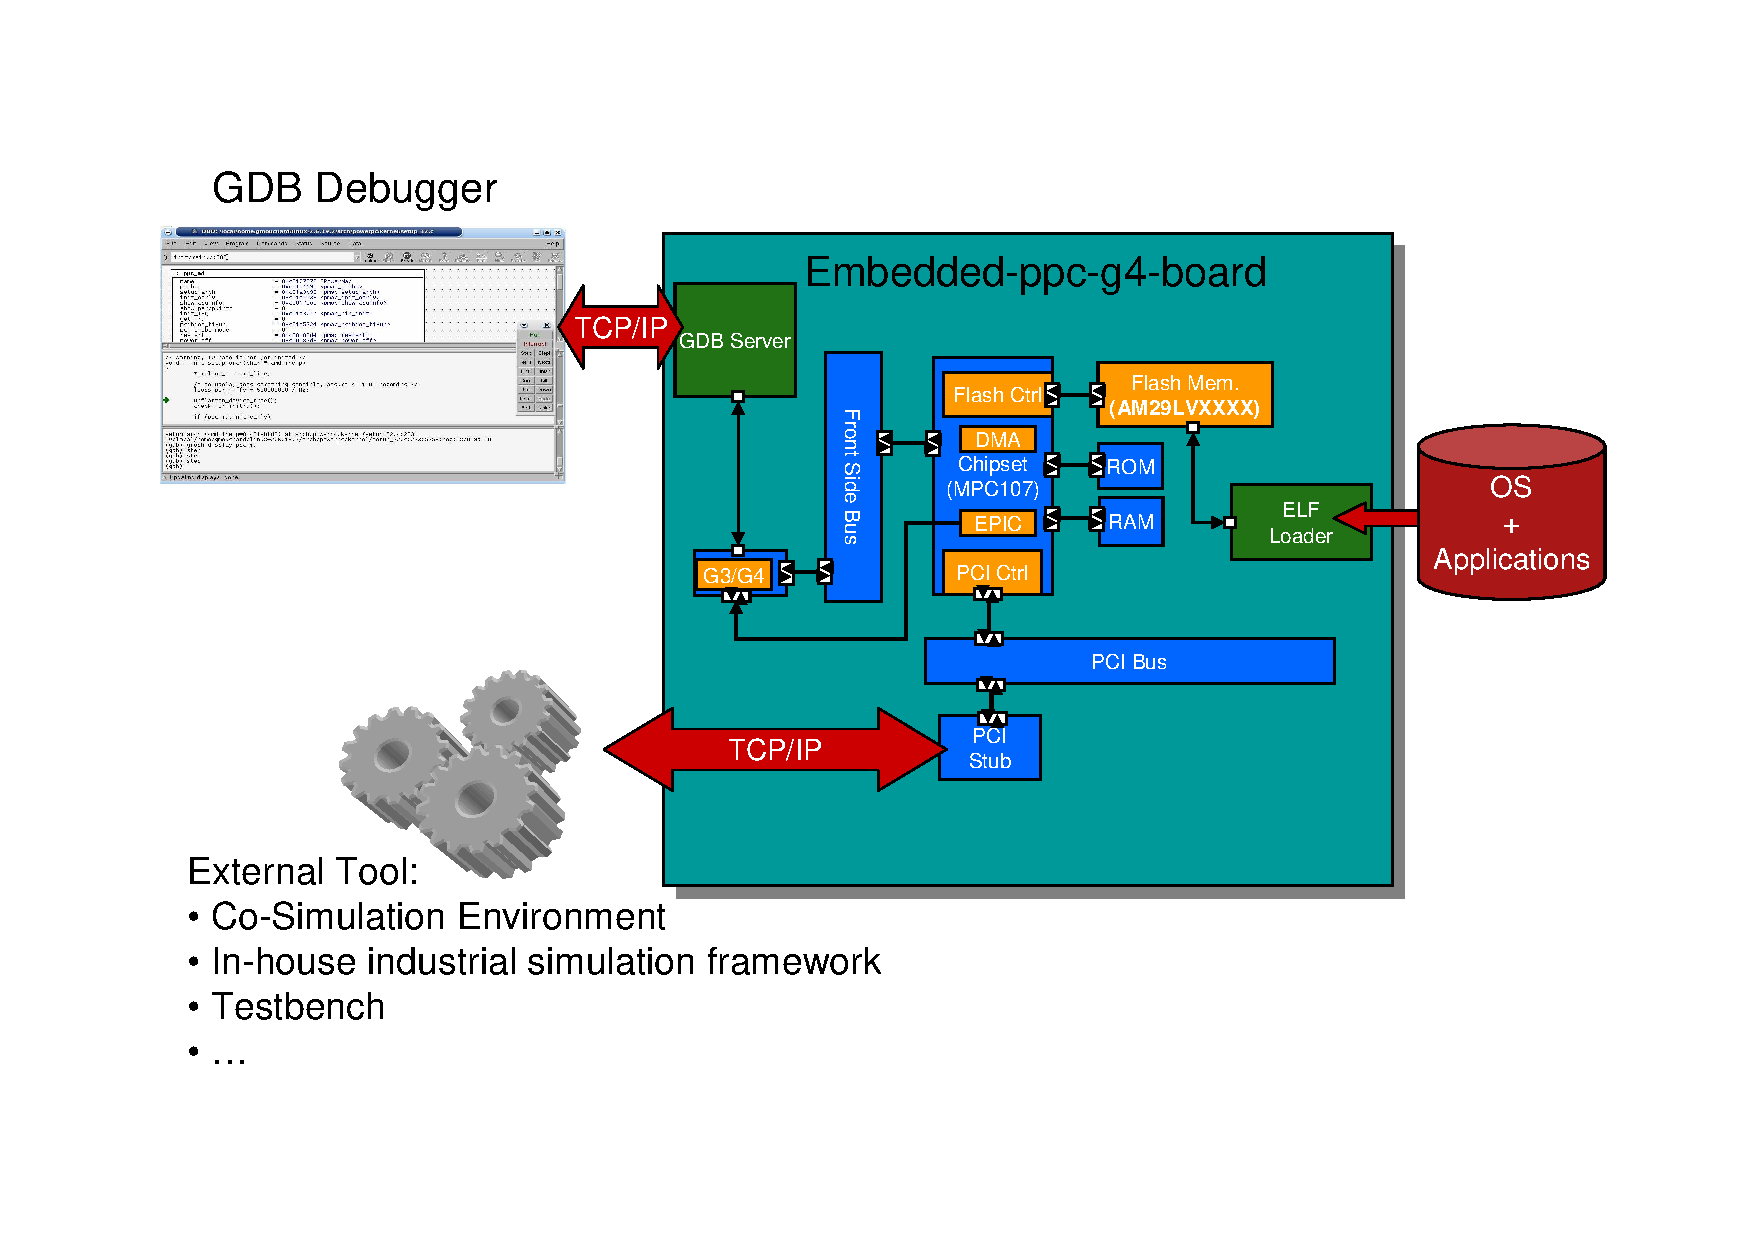
\includegraphics[width=\textwidth]{embedded_ppc_g4_board/fig_schematic.pdf}
	\end{center}
	\caption{UNISIM embedded-ppc-g4-board simulator schematic.}
\end{figure}
\noindent The UNISIM embedded-ppc-g4-board simulator is composed of the following modules and services:
\begin{itemize}\addtolength{\itemsep}{-0.40\baselineskip}
\item \textbf{bus}: Front side bus
\item \textbf{cpu}: PowerPC MPC7447A CPU
\item \textbf{debugger}
\item \textbf{erom}: Memory
\item \textbf{flash}: This module implements an AM29LV800BT flash memory with the following characteristics:\\
Manufacturer ID: 0x010000\\
Device ID word \#0: 0xda2202\\
Size: 4194304 bytes\\
I/O width: 64 bits\\
Number of chips: 4 chips\\
I/O width per chip: 16 bits\\
Size per chip: 1048576 bytes\\
Number of Sectors: 19 sectors\\
8-bit mode support: yes\\
16-bit mode support: yes\\
Access time: 70 ns\\
Byte programming time: 9000 us\\
Word programming time: 110000 us\\
Sector erasing time: 700000000 us\\
Chip erasing time: 14000000000 us\\

\item \textbf{gdb-server}: this service implements the GDB server remote serial protocol over TCP/IP. Standards GDB clients (e.g. gdb, eclipse, ddd) can connect to the simulator to debug the target application that runs within the simulator.
\item \textbf{host-time}: this service is an abstraction layer for the host machine time
\item \textbf{inline-debugger}: this service implements a built-in debugger in the terminal console
\item \textbf{loader}: A multi-format loader that supports ELF32, ELF64, S19, COFF and Raw binary files
\item \textbf{loader.memory-mapper}: A memory mapper
\item \textbf{loader.tee-backtrace}: This service/client implements a tee ('T'). It unifies the backtrace capability of several services that individually provides their own backtrace capability
\item \textbf{loader.tee-blob}: This service/client implements a tee ('T'). It unifies the statement lookup capability of several services that individually provides their own statement lookup capability
\item \textbf{loader.tee-loader}: This service/client implements a tee ('T'). It unifies the loader capability of several services that individually provides their own loader capability
\item \textbf{loader.tee-stmt-lookup}: This service/client implements a tee ('T'). It unifies the statement lookup capability of several services that individually provides their own statement lookup capability
\item \textbf{loader.tee-symbol-table-lookup}: This service/client implements a tee ('T'). It unifies the symbol table lookup capability of several services that individually provides their own symbol table lookup capability
\item \textbf{memory}: Memory
\item \textbf{mpc107}: MPC107 chipset
\item \textbf{mpc107.DMA}: MPC107 integrated Direct Memory Access (DMA) controller
\item \textbf{mpc107.address\_mapper}: MPC107 Address mapper
\item \textbf{mpc107.atu}: MPC107 integrated Address Translation Unit (ATU)
\item \textbf{mpc107.epic}: MPC107 integrated Embedded Programmable Interrupt Controller (EPIC)
\item \textbf{mpc107.pci\_controller}: MPC107 integrated PCI bus controller
\item \textbf{pci-bus}: PCI bus
\item \textbf{pci-stub}: A module that implements a PCI target and acts as a co-simulation stub controlled over a TCP/IP or pipe connection.
\item \textbf{profiler}
\item \textbf{tee-memory-access-reporting}
\item \textbf{tee-memory-access-reporting.tee-memory-access-reporting.control\_selector[0]}
\item \textbf{tee-memory-access-reporting.tee-memory-access-reporting.control\_selector[10]}
\item \textbf{tee-memory-access-reporting.tee-memory-access-reporting.control\_selector[11]}
\item \textbf{tee-memory-access-reporting.tee-memory-access-reporting.control\_selector[12]}
\item \textbf{tee-memory-access-reporting.tee-memory-access-reporting.control\_selector[13]}
\item \textbf{tee-memory-access-reporting.tee-memory-access-reporting.control\_selector[14]}
\item \textbf{tee-memory-access-reporting.tee-memory-access-reporting.control\_selector[15]}
\item \textbf{tee-memory-access-reporting.tee-memory-access-reporting.control\_selector[1]}
\item \textbf{tee-memory-access-reporting.tee-memory-access-reporting.control\_selector[2]}
\item \textbf{tee-memory-access-reporting.tee-memory-access-reporting.control\_selector[3]}
\item \textbf{tee-memory-access-reporting.tee-memory-access-reporting.control\_selector[4]}
\item \textbf{tee-memory-access-reporting.tee-memory-access-reporting.control\_selector[5]}
\item \textbf{tee-memory-access-reporting.tee-memory-access-reporting.control\_selector[6]}
\item \textbf{tee-memory-access-reporting.tee-memory-access-reporting.control\_selector[7]}
\item \textbf{tee-memory-access-reporting.tee-memory-access-reporting.control\_selector[8]}
\item \textbf{tee-memory-access-reporting.tee-memory-access-reporting.control\_selector[9]}
\item \textbf{tee-symbol-table-lookup}: This service/client implements a tee ('T'). It unifies the symbol table lookup capability of several services that individually provides their own symbol table lookup capability
\item \textbf{time}: this service is an abstraction layer for the SystemC kernel time
\end{itemize}
\subsection{Using the UNISIM embedded-ppc-g4-board simulator}
\label{UNISIM embedded-ppc-g4-board_using}
The UNISIM embedded-ppc-g4-board simulator has the following command line options:\\
~\\
\noindent Usage: \texttt{unisim-embedded-ppc-g4-board-1.1beta4 [<options>] [...]}

\noindent Options:
\begin{itemize}
\item \texttt{--set $<$param=value$>$ or -s $<$param=value$>$}: set value of parameter 'param' to 'value'
\item \texttt{--config $<$XML file$>$ or -c $<$XML file$>$}: configures the simulator with the given XML configuration file
\item \texttt{--get-config $<$XML file$>$ or -g $<$XML file$>$}: get the simulator configuration XML file (you can use it to create your own configuration. This option can be combined with -c to get a new configuration file with existing variables from another file
\item \texttt{--list or -l}: lists all available parameters, their type, and their current value
\item \texttt{--warn or -w}: enable printing of kernel warnings
\item \texttt{--doc $<$Latex file$>$ or -d $<$Latex file$>$}: enable printing a latex documentation
\item \texttt{--version or -v}: displays the program version information
\item \texttt{--share-path $<$path$>$ or -p $<$path$>$}: the path that should be used for the share directory (absolute path)
\item \texttt{--help or -h}: displays this help
\end{itemize}
\subsection{Configuration}
\label{UNISIM embedded-ppc-g4-board_configuration}
Simulator configuration (see below) can be modified using command line Options \texttt{--set $<$param=value$>$} or \texttt{--config $<$config file$>$}.\\
~\\
\tablehead{\hline}
\tabletail{\hline}
\begin{supertabular}{|p{7.5cm}|p{7.5cm}|}
\multicolumn{2}{|l|}{\textbf{\Large Global}}\\
\hline
\multicolumn{1}{|p{7.5cm}}{\textbf{Name:} \texttt{enable-gdb-server}} & \multicolumn{1}{p{7.5cm}|}{\textbf{Type:} \texttt{parameter}}\\
\multicolumn{1}{|p{7.5cm}}{\textbf{Default:} \texttt{true}} & \multicolumn{1}{p{7.5cm}|}{\textbf{Data type:} \texttt{boolean}}\\
\multicolumn{2}{|p{15cm}|}{\textbf{Valid:} \texttt{true},~\texttt{false}}\\
\multicolumn{2}{|l|}{}\\
\multicolumn{2}{|p{15cm}|}{\textbf{Description:} \newline Enable/Disable GDB server instantiation.}\\
\hline
\multicolumn{1}{|p{7.5cm}}{\textbf{Name:} \texttt{enable-inline-debugger}} & \multicolumn{1}{p{7.5cm}|}{\textbf{Type:} \texttt{parameter}}\\
\multicolumn{1}{|p{7.5cm}}{\textbf{Default:} \texttt{true}} & \multicolumn{1}{p{7.5cm}|}{\textbf{Data type:} \texttt{boolean}}\\
\multicolumn{2}{|p{15cm}|}{\textbf{Valid:} \texttt{true},~\texttt{false}}\\
\multicolumn{2}{|l|}{}\\
\multicolumn{2}{|p{15cm}|}{\textbf{Description:} \newline Enable/Disable inline debugger instantiation.}\\
\hline
\multicolumn{1}{|p{7.5cm}}{\textbf{Name:} \texttt{enable-press-enter-at-exit}} & \multicolumn{1}{p{7.5cm}|}{\textbf{Type:} \texttt{parameter}}\\
\multicolumn{1}{|p{7.5cm}}{\textbf{Default:} \texttt{false}} & \multicolumn{1}{p{7.5cm}|}{\textbf{Data type:} \texttt{boolean}}\\
\multicolumn{2}{|p{15cm}|}{\textbf{Valid:} \texttt{true},~\texttt{false}}\\
\multicolumn{2}{|l|}{}\\
\multicolumn{2}{|p{15cm}|}{\textbf{Description:} \newline Enable/Disable pressing key enter at exit.}\\
\hline
\multicolumn{1}{|p{7.5cm}}{\textbf{Name:} \texttt{estimate-power}} & \multicolumn{1}{p{7.5cm}|}{\textbf{Type:} \texttt{parameter}}\\
\multicolumn{1}{|p{7.5cm}}{\textbf{Default:} \texttt{false}} & \multicolumn{1}{p{7.5cm}|}{\textbf{Data type:} \texttt{boolean}}\\
\multicolumn{2}{|p{15cm}|}{\textbf{Valid:} \texttt{true},~\texttt{false}}\\
\multicolumn{2}{|l|}{}\\
\multicolumn{2}{|p{15cm}|}{\textbf{Description:} \newline Enable/Disable power estimators instantiation.}\\
\hline
\multicolumn{1}{|p{7.5cm}}{\textbf{Name:} \texttt{kernel\_logger.file}} & \multicolumn{1}{p{7.5cm}|}{\textbf{Type:} \texttt{parameter}}\\
\multicolumn{1}{|p{7.5cm}}{\textbf{Default:} \texttt{false}} & \multicolumn{1}{p{7.5cm}|}{\textbf{Data type:} \texttt{boolean}}\\
\multicolumn{2}{|p{15cm}|}{\textbf{Valid:} \texttt{true},~\texttt{false}}\\
\multicolumn{2}{|l|}{}\\
\multicolumn{2}{|p{15cm}|}{\textbf{Description:} \newline Keep logger output in a file.}\\
\hline
\multicolumn{1}{|p{7.5cm}}{\textbf{Name:} \texttt{kernel\_logger.filename}} & \multicolumn{1}{p{7.5cm}|}{\textbf{Type:} \texttt{parameter}}\\
\multicolumn{1}{|p{7.5cm}}{\textbf{Default:} \texttt{logger\_output.txt}} & \multicolumn{1}{p{7.5cm}|}{\textbf{Data type:} \texttt{string}}\\
\multicolumn{2}{|l|}{}\\
\multicolumn{2}{|l|}{}\\
\multicolumn{2}{|p{15cm}|}{\textbf{Description:} \newline Filename to keep logger output \_(the option file must be activated).}\\
\hline
\multicolumn{1}{|p{7.5cm}}{\textbf{Name:} \texttt{kernel\_logger.std\_err}} & \multicolumn{1}{p{7.5cm}|}{\textbf{Type:} \texttt{parameter}}\\
\multicolumn{1}{|p{7.5cm}}{\textbf{Default:} \texttt{true}} & \multicolumn{1}{p{7.5cm}|}{\textbf{Data type:} \texttt{boolean}}\\
\multicolumn{2}{|p{15cm}|}{\textbf{Valid:} \texttt{true},~\texttt{false}}\\
\multicolumn{2}{|l|}{}\\
\multicolumn{2}{|p{15cm}|}{\textbf{Description:} \newline Show logger output through the standard error output.}\\
\hline
\multicolumn{1}{|p{7.5cm}}{\textbf{Name:} \texttt{kernel\_logger.std\_err\_color}} & \multicolumn{1}{p{7.5cm}|}{\textbf{Type:} \texttt{parameter}}\\
\multicolumn{1}{|p{7.5cm}}{\textbf{Default:} \texttt{false}} & \multicolumn{1}{p{7.5cm}|}{\textbf{Data type:} \texttt{boolean}}\\
\multicolumn{2}{|p{15cm}|}{\textbf{Valid:} \texttt{true},~\texttt{false}}\\
\multicolumn{2}{|l|}{}\\
\multicolumn{2}{|p{15cm}|}{\textbf{Description:} \newline Colorize logger output through the standard error output \_(only works if std\_err is active).}\\
\hline
\multicolumn{1}{|p{7.5cm}}{\textbf{Name:} \texttt{kernel\_logger.std\_out}} & \multicolumn{1}{p{7.5cm}|}{\textbf{Type:} \texttt{parameter}}\\
\multicolumn{1}{|p{7.5cm}}{\textbf{Default:} \texttt{false}} & \multicolumn{1}{p{7.5cm}|}{\textbf{Data type:} \texttt{boolean}}\\
\multicolumn{2}{|p{15cm}|}{\textbf{Valid:} \texttt{true},~\texttt{false}}\\
\multicolumn{2}{|l|}{}\\
\multicolumn{2}{|p{15cm}|}{\textbf{Description:} \newline Show logger output through the standard output.}\\
\hline
\multicolumn{1}{|p{7.5cm}}{\textbf{Name:} \texttt{kernel\_logger.std\_out\_color}} & \multicolumn{1}{p{7.5cm}|}{\textbf{Type:} \texttt{parameter}}\\
\multicolumn{1}{|p{7.5cm}}{\textbf{Default:} \texttt{false}} & \multicolumn{1}{p{7.5cm}|}{\textbf{Data type:} \texttt{boolean}}\\
\multicolumn{2}{|p{15cm}|}{\textbf{Valid:} \texttt{true},~\texttt{false}}\\
\multicolumn{2}{|l|}{}\\
\multicolumn{2}{|p{15cm}|}{\textbf{Description:} \newline Colorize logger output through the standard output \_(only works if std\_out is active).}\\
\hline
\multicolumn{1}{|p{7.5cm}}{\textbf{Name:} \texttt{kernel\_logger.xml\_file}} & \multicolumn{1}{p{7.5cm}|}{\textbf{Type:} \texttt{parameter}}\\
\multicolumn{1}{|p{7.5cm}}{\textbf{Default:} \texttt{false}} & \multicolumn{1}{p{7.5cm}|}{\textbf{Data type:} \texttt{boolean}}\\
\multicolumn{2}{|p{15cm}|}{\textbf{Valid:} \texttt{true},~\texttt{false}}\\
\multicolumn{2}{|l|}{}\\
\multicolumn{2}{|p{15cm}|}{\textbf{Description:} \newline Keep logger output in a file xml formatted.}\\
\hline
\multicolumn{1}{|p{7.5cm}}{\textbf{Name:} \texttt{kernel\_logger.xml\_file\_gzipped}} & \multicolumn{1}{p{7.5cm}|}{\textbf{Type:} \texttt{parameter}}\\
\multicolumn{1}{|p{7.5cm}}{\textbf{Default:} \texttt{false}} & \multicolumn{1}{p{7.5cm}|}{\textbf{Data type:} \texttt{boolean}}\\
\multicolumn{2}{|p{15cm}|}{\textbf{Valid:} \texttt{true},~\texttt{false}}\\
\multicolumn{2}{|l|}{}\\
\multicolumn{2}{|p{15cm}|}{\textbf{Description:} \newline If the xml\_file option is active, the output file will be compressed (a .gz extension will be automatically added to the xml\_filename option.}\\
\hline
\multicolumn{1}{|p{7.5cm}}{\textbf{Name:} \texttt{kernel\_logger.xml\_filename}} & \multicolumn{1}{p{7.5cm}|}{\textbf{Type:} \texttt{parameter}}\\
\multicolumn{1}{|p{7.5cm}}{\textbf{Default:} \texttt{logger\_output.xml}} & \multicolumn{1}{p{7.5cm}|}{\textbf{Data type:} \texttt{string}}\\
\multicolumn{2}{|l|}{}\\
\multicolumn{2}{|l|}{}\\
\multicolumn{2}{|p{15cm}|}{\textbf{Description:} \newline Filename to keep logger xml output \_(the option xml\_file must be activated).}\\
\hline
\multicolumn{1}{|p{7.5cm}}{\textbf{Name:} \texttt{message-spy}} & \multicolumn{1}{p{7.5cm}|}{\textbf{Type:} \texttt{parameter}}\\
\multicolumn{1}{|p{7.5cm}}{\textbf{Default:} \texttt{false}} & \multicolumn{1}{p{7.5cm}|}{\textbf{Data type:} \texttt{boolean}}\\
\multicolumn{2}{|p{15cm}|}{\textbf{Valid:} \texttt{true},~\texttt{false}}\\
\multicolumn{2}{|l|}{}\\
\multicolumn{2}{|p{15cm}|}{\textbf{Description:} \newline Enable/Disable message spies instantiation.}\\
\hline
\hline
\multicolumn{2}{|l|}{\textbf{\Large bus}}\\
\hline
\multicolumn{1}{|p{7.5cm}}{\textbf{Name:} \texttt{bus.verbose}} & \multicolumn{1}{p{7.5cm}|}{\textbf{Type:} \texttt{parameter}}\\
\multicolumn{1}{|p{7.5cm}}{\textbf{Default:} \texttt{false}} & \multicolumn{1}{p{7.5cm}|}{\textbf{Data type:} \texttt{boolean}}\\
\multicolumn{2}{|p{15cm}|}{\textbf{Valid:} \texttt{true},~\texttt{false}}\\
\multicolumn{2}{|l|}{}\\
\multicolumn{2}{|p{15cm}|}{\textbf{Description:} \newline enable/disable verbosity.}\\
\hline
\multicolumn{1}{|p{7.5cm}}{\textbf{Name:} \texttt{bus.cycle-time}} & \multicolumn{1}{p{7.5cm}|}{\textbf{Type:} \texttt{parameter}}\\
\multicolumn{1}{|p{7.5cm}}{\textbf{Default:} \texttt{13332 ps}} & \multicolumn{1}{p{7.5cm}|}{\textbf{Data type:} \texttt{sc\_time}}\\
\multicolumn{2}{|l|}{}\\
\multicolumn{2}{|l|}{}\\
\multicolumn{2}{|p{15cm}|}{\textbf{Description:} \newline cycle time.}\\
\hline
\hline
\multicolumn{2}{|l|}{\textbf{\Large cpu}}\\
\hline
\multicolumn{1}{|p{7.5cm}}{\textbf{Name:} \texttt{cpu.cpu-cycle-time}} & \multicolumn{1}{p{7.5cm}|}{\textbf{Type:} \texttt{parameter}}\\
\multicolumn{1}{|p{7.5cm}}{\textbf{Default:} \texttt{3333}} & \multicolumn{1}{p{7.5cm}|}{\textbf{Data type:} \texttt{unsigned 64-bit integer}}\\
\multicolumn{2}{|l|}{}\\
\multicolumn{2}{|l|}{}\\
\multicolumn{2}{|p{15cm}|}{\textbf{Description:} \newline CPU cycle time in picoseconds.}\\
\hline
\multicolumn{1}{|p{7.5cm}}{\textbf{Name:} \texttt{cpu.voltage}} & \multicolumn{1}{p{7.5cm}|}{\textbf{Type:} \texttt{parameter}}\\
\multicolumn{1}{|p{7.5cm}}{\textbf{Default:} \texttt{1300}} & \multicolumn{1}{p{7.5cm}|}{\textbf{Data type:} \texttt{unsigned 64-bit integer}}\\
\multicolumn{2}{|l|}{}\\
\multicolumn{2}{|l|}{}\\
\multicolumn{2}{|p{15cm}|}{\textbf{Description:} \newline CPU voltage in mV.}\\
\hline
\multicolumn{1}{|p{7.5cm}}{\textbf{Name:} \texttt{cpu.max-inst}} & \multicolumn{1}{p{7.5cm}|}{\textbf{Type:} \texttt{parameter}}\\
\multicolumn{1}{|p{7.5cm}}{\textbf{Default:} \texttt{18446744073709551615}} & \multicolumn{1}{p{7.5cm}|}{\textbf{Data type:} \texttt{unsigned 64-bit integer}}\\
\multicolumn{2}{|l|}{}\\
\multicolumn{2}{|l|}{}\\
\multicolumn{2}{|p{15cm}|}{\textbf{Description:} \newline maximum number of instructions to simulate.}\\
\hline
\multicolumn{1}{|p{7.5cm}}{\textbf{Name:} \texttt{cpu.verbose-all}} & \multicolumn{1}{p{7.5cm}|}{\textbf{Type:} \texttt{parameter}}\\
\multicolumn{1}{|p{7.5cm}}{\textbf{Default:} \texttt{false}} & \multicolumn{1}{p{7.5cm}|}{\textbf{Data type:} \texttt{boolean}}\\
\multicolumn{2}{|p{15cm}|}{\textbf{Valid:} \texttt{true},~\texttt{false}}\\
\multicolumn{2}{|l|}{}\\
\multicolumn{2}{|p{15cm}|}{\textbf{Description:} \newline globally enable/disable verbosity.}\\
\hline
\multicolumn{1}{|p{7.5cm}}{\textbf{Name:} \texttt{cpu.verbose-setup}} & \multicolumn{1}{p{7.5cm}|}{\textbf{Type:} \texttt{parameter}}\\
\multicolumn{1}{|p{7.5cm}}{\textbf{Default:} \texttt{false}} & \multicolumn{1}{p{7.5cm}|}{\textbf{Data type:} \texttt{boolean}}\\
\multicolumn{2}{|p{15cm}|}{\textbf{Valid:} \texttt{true},~\texttt{false}}\\
\multicolumn{2}{|l|}{}\\
\multicolumn{2}{|p{15cm}|}{\textbf{Description:} \newline enable/disable verbosity while setup.}\\
\hline
\multicolumn{1}{|p{7.5cm}}{\textbf{Name:} \texttt{cpu.verbose-step}} & \multicolumn{1}{p{7.5cm}|}{\textbf{Type:} \texttt{parameter}}\\
\multicolumn{1}{|p{7.5cm}}{\textbf{Default:} \texttt{false}} & \multicolumn{1}{p{7.5cm}|}{\textbf{Data type:} \texttt{boolean}}\\
\multicolumn{2}{|p{15cm}|}{\textbf{Valid:} \texttt{true},~\texttt{false}}\\
\multicolumn{2}{|l|}{}\\
\multicolumn{2}{|p{15cm}|}{\textbf{Description:} \newline enable/disable verbosity when simulating an instruction.}\\
\hline
\multicolumn{1}{|p{7.5cm}}{\textbf{Name:} \texttt{cpu.verbose-dtlb}} & \multicolumn{1}{p{7.5cm}|}{\textbf{Type:} \texttt{parameter}}\\
\multicolumn{1}{|p{7.5cm}}{\textbf{Default:} \texttt{false}} & \multicolumn{1}{p{7.5cm}|}{\textbf{Data type:} \texttt{boolean}}\\
\multicolumn{2}{|p{15cm}|}{\textbf{Valid:} \texttt{true},~\texttt{false}}\\
\multicolumn{2}{|l|}{}\\
\multicolumn{2}{|p{15cm}|}{\textbf{Description:} \newline enable/disable verbosity when accessing data translation lookahead buffer.}\\
\hline
\multicolumn{1}{|p{7.5cm}}{\textbf{Name:} \texttt{cpu.verbose-itlb}} & \multicolumn{1}{p{7.5cm}|}{\textbf{Type:} \texttt{parameter}}\\
\multicolumn{1}{|p{7.5cm}}{\textbf{Default:} \texttt{false}} & \multicolumn{1}{p{7.5cm}|}{\textbf{Data type:} \texttt{boolean}}\\
\multicolumn{2}{|p{15cm}|}{\textbf{Valid:} \texttt{true},~\texttt{false}}\\
\multicolumn{2}{|l|}{}\\
\multicolumn{2}{|p{15cm}|}{\textbf{Description:} \newline enable/disable verbosity when accessing instruction translation lookahead buffer.}\\
\hline
\multicolumn{1}{|p{7.5cm}}{\textbf{Name:} \texttt{cpu.verbose-dl1}} & \multicolumn{1}{p{7.5cm}|}{\textbf{Type:} \texttt{parameter}}\\
\multicolumn{1}{|p{7.5cm}}{\textbf{Default:} \texttt{false}} & \multicolumn{1}{p{7.5cm}|}{\textbf{Data type:} \texttt{boolean}}\\
\multicolumn{2}{|p{15cm}|}{\textbf{Valid:} \texttt{true},~\texttt{false}}\\
\multicolumn{2}{|l|}{}\\
\multicolumn{2}{|p{15cm}|}{\textbf{Description:} \newline enable/disable verbosity when accessing L1 data cache.}\\
\hline
\multicolumn{1}{|p{7.5cm}}{\textbf{Name:} \texttt{cpu.verbose-il1}} & \multicolumn{1}{p{7.5cm}|}{\textbf{Type:} \texttt{parameter}}\\
\multicolumn{1}{|p{7.5cm}}{\textbf{Default:} \texttt{false}} & \multicolumn{1}{p{7.5cm}|}{\textbf{Data type:} \texttt{boolean}}\\
\multicolumn{2}{|p{15cm}|}{\textbf{Valid:} \texttt{true},~\texttt{false}}\\
\multicolumn{2}{|l|}{}\\
\multicolumn{2}{|p{15cm}|}{\textbf{Description:} \newline enable/disable verbosity when accessing L1 instruction cache.}\\
\hline
\multicolumn{1}{|p{7.5cm}}{\textbf{Name:} \texttt{cpu.verbose-l2}} & \multicolumn{1}{p{7.5cm}|}{\textbf{Type:} \texttt{parameter}}\\
\multicolumn{1}{|p{7.5cm}}{\textbf{Default:} \texttt{false}} & \multicolumn{1}{p{7.5cm}|}{\textbf{Data type:} \texttt{boolean}}\\
\multicolumn{2}{|p{15cm}|}{\textbf{Valid:} \texttt{true},~\texttt{false}}\\
\multicolumn{2}{|l|}{}\\
\multicolumn{2}{|p{15cm}|}{\textbf{Description:} \newline enable/disable verbosity when accessing L2 unified cache.}\\
\hline
\multicolumn{1}{|p{7.5cm}}{\textbf{Name:} \texttt{cpu.verbose-load}} & \multicolumn{1}{p{7.5cm}|}{\textbf{Type:} \texttt{parameter}}\\
\multicolumn{1}{|p{7.5cm}}{\textbf{Default:} \texttt{false}} & \multicolumn{1}{p{7.5cm}|}{\textbf{Data type:} \texttt{boolean}}\\
\multicolumn{2}{|p{15cm}|}{\textbf{Valid:} \texttt{true},~\texttt{false}}\\
\multicolumn{2}{|l|}{}\\
\multicolumn{2}{|p{15cm}|}{\textbf{Description:} \newline enable/disable verbosity when simulating a load.}\\
\hline
\multicolumn{1}{|p{7.5cm}}{\textbf{Name:} \texttt{cpu.verbose-store}} & \multicolumn{1}{p{7.5cm}|}{\textbf{Type:} \texttt{parameter}}\\
\multicolumn{1}{|p{7.5cm}}{\textbf{Default:} \texttt{false}} & \multicolumn{1}{p{7.5cm}|}{\textbf{Data type:} \texttt{boolean}}\\
\multicolumn{2}{|p{15cm}|}{\textbf{Valid:} \texttt{true},~\texttt{false}}\\
\multicolumn{2}{|l|}{}\\
\multicolumn{2}{|p{15cm}|}{\textbf{Description:} \newline enable/disable verbosity when simulating a store.}\\
\hline
\multicolumn{1}{|p{7.5cm}}{\textbf{Name:} \texttt{cpu.verbose-read-memory}} & \multicolumn{1}{p{7.5cm}|}{\textbf{Type:} \texttt{parameter}}\\
\multicolumn{1}{|p{7.5cm}}{\textbf{Default:} \texttt{false}} & \multicolumn{1}{p{7.5cm}|}{\textbf{Data type:} \texttt{boolean}}\\
\multicolumn{2}{|p{15cm}|}{\textbf{Valid:} \texttt{true},~\texttt{false}}\\
\multicolumn{2}{|l|}{}\\
\multicolumn{2}{|p{15cm}|}{\textbf{Description:} \newline enable/disable verbosity when reading memory for a debug purpose.}\\
\hline
\multicolumn{1}{|p{7.5cm}}{\textbf{Name:} \texttt{cpu.verbose-write-memory}} & \multicolumn{1}{p{7.5cm}|}{\textbf{Type:} \texttt{parameter}}\\
\multicolumn{1}{|p{7.5cm}}{\textbf{Default:} \texttt{false}} & \multicolumn{1}{p{7.5cm}|}{\textbf{Data type:} \texttt{boolean}}\\
\multicolumn{2}{|p{15cm}|}{\textbf{Valid:} \texttt{true},~\texttt{false}}\\
\multicolumn{2}{|l|}{}\\
\multicolumn{2}{|p{15cm}|}{\textbf{Description:} \newline enable/disable verbosity when writing memory for a debug purpose.}\\
\hline
\multicolumn{1}{|p{7.5cm}}{\textbf{Name:} \texttt{cpu.verbose-exception}} & \multicolumn{1}{p{7.5cm}|}{\textbf{Type:} \texttt{parameter}}\\
\multicolumn{1}{|p{7.5cm}}{\textbf{Default:} \texttt{false}} & \multicolumn{1}{p{7.5cm}|}{\textbf{Data type:} \texttt{boolean}}\\
\multicolumn{2}{|p{15cm}|}{\textbf{Valid:} \texttt{true},~\texttt{false}}\\
\multicolumn{2}{|l|}{}\\
\multicolumn{2}{|p{15cm}|}{\textbf{Description:} \newline enable/disable verbosity when handling exceptions.}\\
\hline
\multicolumn{1}{|p{7.5cm}}{\textbf{Name:} \texttt{cpu.verbose-set-msr}} & \multicolumn{1}{p{7.5cm}|}{\textbf{Type:} \texttt{parameter}}\\
\multicolumn{1}{|p{7.5cm}}{\textbf{Default:} \texttt{false}} & \multicolumn{1}{p{7.5cm}|}{\textbf{Data type:} \texttt{boolean}}\\
\multicolumn{2}{|p{15cm}|}{\textbf{Valid:} \texttt{true},~\texttt{false}}\\
\multicolumn{2}{|l|}{}\\
\multicolumn{2}{|p{15cm}|}{\textbf{Description:} \newline enable/disable verbosity when setting MSR.}\\
\hline
\multicolumn{1}{|p{7.5cm}}{\textbf{Name:} \texttt{cpu.verbose-set-hid0}} & \multicolumn{1}{p{7.5cm}|}{\textbf{Type:} \texttt{parameter}}\\
\multicolumn{1}{|p{7.5cm}}{\textbf{Default:} \texttt{false}} & \multicolumn{1}{p{7.5cm}|}{\textbf{Data type:} \texttt{boolean}}\\
\multicolumn{2}{|p{15cm}|}{\textbf{Valid:} \texttt{true},~\texttt{false}}\\
\multicolumn{2}{|l|}{}\\
\multicolumn{2}{|p{15cm}|}{\textbf{Description:} \newline enable/disable verbosity when setting HID0.}\\
\hline
\multicolumn{1}{|p{7.5cm}}{\textbf{Name:} \texttt{cpu.verbose-set-hid1}} & \multicolumn{1}{p{7.5cm}|}{\textbf{Type:} \texttt{parameter}}\\
\multicolumn{1}{|p{7.5cm}}{\textbf{Default:} \texttt{false}} & \multicolumn{1}{p{7.5cm}|}{\textbf{Data type:} \texttt{boolean}}\\
\multicolumn{2}{|p{15cm}|}{\textbf{Valid:} \texttt{true},~\texttt{false}}\\
\multicolumn{2}{|l|}{}\\
\multicolumn{2}{|p{15cm}|}{\textbf{Description:} \newline enable/disable verbosity when setting HID1.}\\
\hline
\multicolumn{1}{|p{7.5cm}}{\textbf{Name:} \texttt{cpu.verbose-set-hid2}} & \multicolumn{1}{p{7.5cm}|}{\textbf{Type:} \texttt{parameter}}\\
\multicolumn{1}{|p{7.5cm}}{\textbf{Default:} \texttt{false}} & \multicolumn{1}{p{7.5cm}|}{\textbf{Data type:} \texttt{boolean}}\\
\multicolumn{2}{|p{15cm}|}{\textbf{Valid:} \texttt{true},~\texttt{false}}\\
\multicolumn{2}{|l|}{}\\
\multicolumn{2}{|p{15cm}|}{\textbf{Description:} \newline enable/disable verbosity when setting HID2.}\\
\hline
\multicolumn{1}{|p{7.5cm}}{\textbf{Name:} \texttt{cpu.verbose-set-l2cr}} & \multicolumn{1}{p{7.5cm}|}{\textbf{Type:} \texttt{parameter}}\\
\multicolumn{1}{|p{7.5cm}}{\textbf{Default:} \texttt{false}} & \multicolumn{1}{p{7.5cm}|}{\textbf{Data type:} \texttt{boolean}}\\
\multicolumn{2}{|p{15cm}|}{\textbf{Valid:} \texttt{true},~\texttt{false}}\\
\multicolumn{2}{|l|}{}\\
\multicolumn{2}{|p{15cm}|}{\textbf{Description:} \newline enable/disable verbosity when setting L2CR.}\\
\hline
\multicolumn{1}{|p{7.5cm}}{\textbf{Name:} \texttt{cpu.enable-linux-printk-snooping}} & \multicolumn{1}{p{7.5cm}|}{\textbf{Type:} \texttt{parameter}}\\
\multicolumn{1}{|p{7.5cm}}{\textbf{Default:} \texttt{false}} & \multicolumn{1}{p{7.5cm}|}{\textbf{Data type:} \texttt{boolean}}\\
\multicolumn{2}{|p{15cm}|}{\textbf{Valid:} \texttt{true},~\texttt{false}}\\
\multicolumn{2}{|l|}{}\\
\multicolumn{2}{|p{15cm}|}{\textbf{Description:} \newline enable/disable linux printk buffer snooping.}\\
\hline
\multicolumn{1}{|p{7.5cm}}{\textbf{Name:} \texttt{cpu.enable-linux-syscall-snooping}} & \multicolumn{1}{p{7.5cm}|}{\textbf{Type:} \texttt{parameter}}\\
\multicolumn{1}{|p{7.5cm}}{\textbf{Default:} \texttt{false}} & \multicolumn{1}{p{7.5cm}|}{\textbf{Data type:} \texttt{boolean}}\\
\multicolumn{2}{|p{15cm}|}{\textbf{Valid:} \texttt{true},~\texttt{false}}\\
\multicolumn{2}{|l|}{}\\
\multicolumn{2}{|p{15cm}|}{\textbf{Description:} \newline enable/disable linux syscall snooping.}\\
\hline
\multicolumn{1}{|p{7.5cm}}{\textbf{Name:} \texttt{cpu.trap-on-instruction-counter}} & \multicolumn{1}{p{7.5cm}|}{\textbf{Type:} \texttt{parameter}}\\
\multicolumn{1}{|p{7.5cm}}{\textbf{Default:} \texttt{18446744073709551615}} & \multicolumn{1}{p{7.5cm}|}{\textbf{Data type:} \texttt{unsigned 64-bit integer}}\\
\multicolumn{2}{|l|}{}\\
\multicolumn{2}{|l|}{}\\
\multicolumn{2}{|p{15cm}|}{\textbf{Description:} \newline number of simulated instruction before traping.}\\
\hline
\multicolumn{1}{|p{7.5cm}}{\textbf{Name:} \texttt{cpu.halt-on}} & \multicolumn{1}{p{7.5cm}|}{\textbf{Type:} \texttt{parameter}}\\
\multicolumn{1}{|p{7.5cm}}{\textbf{Default:} \texttt{}} & \multicolumn{1}{p{7.5cm}|}{\textbf{Data type:} \texttt{string}}\\
\multicolumn{2}{|l|}{}\\
\multicolumn{2}{|l|}{}\\
\multicolumn{2}{|p{15cm}|}{\textbf{Description:} \newline Symbol or address where to stop simulation.}\\
\hline
\multicolumn{1}{|p{7.5cm}}{\textbf{Name:} \texttt{cpu.bus-cycle-time}} & \multicolumn{1}{p{7.5cm}|}{\textbf{Type:} \texttt{parameter}}\\
\multicolumn{1}{|p{7.5cm}}{\textbf{Default:} \texttt{13332 ps}} & \multicolumn{1}{p{7.5cm}|}{\textbf{Data type:} \texttt{sc\_time}}\\
\multicolumn{2}{|l|}{}\\
\multicolumn{2}{|l|}{}\\
\multicolumn{2}{|p{15cm}|}{\textbf{Description:} \newline bus cycle time.}\\
\hline
\multicolumn{1}{|p{7.5cm}}{\textbf{Name:} \texttt{cpu.nice-time}} & \multicolumn{1}{p{7.5cm}|}{\textbf{Type:} \texttt{parameter}}\\
\multicolumn{1}{|p{7.5cm}}{\textbf{Default:} \texttt{1 ms}} & \multicolumn{1}{p{7.5cm}|}{\textbf{Data type:} \texttt{sc\_time}}\\
\multicolumn{2}{|l|}{}\\
\multicolumn{2}{|l|}{}\\
\multicolumn{2}{|p{15cm}|}{\textbf{Description:} \newline maximum time between synchonizations.}\\
\hline
\multicolumn{1}{|p{7.5cm}}{\textbf{Name:} \texttt{cpu.ipc}} & \multicolumn{1}{p{7.5cm}|}{\textbf{Type:} \texttt{parameter}}\\
\multicolumn{1}{|p{7.5cm}}{\textbf{Default:} \texttt{1}} & \multicolumn{1}{p{7.5cm}|}{\textbf{Data type:} \texttt{double precision floating-point}}\\
\multicolumn{2}{|l|}{}\\
\multicolumn{2}{|l|}{}\\
\multicolumn{2}{|p{15cm}|}{\textbf{Description:} \newline targeted average instructions per second.}\\
\hline
\multicolumn{1}{|p{7.5cm}}{\textbf{Name:} \texttt{cpu.enable-host-idle}} & \multicolumn{1}{p{7.5cm}|}{\textbf{Type:} \texttt{parameter}}\\
\multicolumn{1}{|p{7.5cm}}{\textbf{Default:} \texttt{false}} & \multicolumn{1}{p{7.5cm}|}{\textbf{Data type:} \texttt{boolean}}\\
\multicolumn{2}{|p{15cm}|}{\textbf{Valid:} \texttt{true},~\texttt{false}}\\
\multicolumn{2}{|l|}{}\\
\multicolumn{2}{|p{15cm}|}{\textbf{Description:} \newline Enable/Disable host idle periods when target is idle.}\\
\hline
\hline
\multicolumn{2}{|l|}{\textbf{\Large debugger}}\\
\hline
\multicolumn{1}{|p{7.5cm}}{\textbf{Name:} \texttt{debugger.verbose}} & \multicolumn{1}{p{7.5cm}|}{\textbf{Type:} \texttt{parameter}}\\
\multicolumn{1}{|p{7.5cm}}{\textbf{Default:} \texttt{false}} & \multicolumn{1}{p{7.5cm}|}{\textbf{Data type:} \texttt{boolean}}\\
\multicolumn{2}{|p{15cm}|}{\textbf{Valid:} \texttt{true},~\texttt{false}}\\
\multicolumn{2}{|l|}{}\\
\multicolumn{2}{|p{15cm}|}{\textbf{Description:} \newline Enable/Disable verbosity.}\\
\hline
\multicolumn{1}{|p{7.5cm}}{\textbf{Name:} \texttt{debugger.dwarf-to-html-output-} \newline$\hookrightarrow$\texttt{directory}} & \multicolumn{1}{p{7.5cm}|}{\textbf{Type:} \texttt{parameter}}\\
\multicolumn{1}{|p{7.5cm}}{\textbf{Default:} \texttt{}} & \multicolumn{1}{p{7.5cm}|}{\textbf{Data type:} \texttt{string}}\\
\multicolumn{2}{|l|}{}\\
\multicolumn{2}{|l|}{}\\
\multicolumn{2}{|p{15cm}|}{\textbf{Description:} \newline DWARF v2/v3 to HTML output directory.}\\
\hline
\multicolumn{1}{|p{7.5cm}}{\textbf{Name:} \texttt{debugger.dwarf-register-number-} \newline$\hookrightarrow$\texttt{mapping-filename}} & \multicolumn{1}{p{7.5cm}|}{\textbf{Type:} \texttt{parameter}}\\
\multicolumn{1}{|p{7.5cm}}{\textbf{Default:} \texttt{powerpc\_eabi\_gcc\_dwarf\_register\_} \newline$\hookrightarrow$\texttt{number\_mapping.xml}} & \multicolumn{1}{p{7.5cm}|}{\textbf{Data type:} \texttt{string}}\\
\multicolumn{2}{|l|}{}\\
\multicolumn{2}{|l|}{}\\
\multicolumn{2}{|p{15cm}|}{\textbf{Description:} \newline DWARF register number mapping filename.}\\
\hline
\multicolumn{1}{|p{7.5cm}}{\textbf{Name:} \texttt{debugger.parse-dwarf}} & \multicolumn{1}{p{7.5cm}|}{\textbf{Type:} \texttt{parameter}}\\
\multicolumn{1}{|p{7.5cm}}{\textbf{Default:} \texttt{true}} & \multicolumn{1}{p{7.5cm}|}{\textbf{Data type:} \texttt{boolean}}\\
\multicolumn{2}{|p{15cm}|}{\textbf{Valid:} \texttt{true},~\texttt{false}}\\
\multicolumn{2}{|l|}{}\\
\multicolumn{2}{|p{15cm}|}{\textbf{Description:} \newline Enable/Disable parsing of DWARF debugging informations.}\\
\hline
\multicolumn{1}{|p{7.5cm}}{\textbf{Name:} \texttt{debugger.debug-dwarf}} & \multicolumn{1}{p{7.5cm}|}{\textbf{Type:} \texttt{parameter}}\\
\multicolumn{1}{|p{7.5cm}}{\textbf{Default:} \texttt{false}} & \multicolumn{1}{p{7.5cm}|}{\textbf{Data type:} \texttt{boolean}}\\
\multicolumn{2}{|p{15cm}|}{\textbf{Valid:} \texttt{true},~\texttt{false}}\\
\multicolumn{2}{|l|}{}\\
\multicolumn{2}{|p{15cm}|}{\textbf{Description:} \newline Enable/Disable debugging of DWARF.}\\
\hline
\hline
\multicolumn{2}{|l|}{\textbf{\Large erom}}\\
\hline
\multicolumn{1}{|p{7.5cm}}{\textbf{Name:} \texttt{erom.org}} & \multicolumn{1}{p{7.5cm}|}{\textbf{Type:} \texttt{parameter}}\\
\multicolumn{1}{|p{7.5cm}}{\textbf{Default:} \texttt{0x78000000}} & \multicolumn{1}{p{7.5cm}|}{\textbf{Data type:} \texttt{unsigned 32-bit integer}}\\
\multicolumn{2}{|l|}{}\\
\multicolumn{2}{|l|}{}\\
\multicolumn{2}{|p{15cm}|}{\textbf{Description:} \newline memory origin/base address.}\\
\hline
\multicolumn{1}{|p{7.5cm}}{\textbf{Name:} \texttt{erom.bytesize}} & \multicolumn{1}{p{7.5cm}|}{\textbf{Type:} \texttt{parameter}}\\
\multicolumn{1}{|p{7.5cm}}{\textbf{Default:} \texttt{16777216}} & \multicolumn{1}{p{7.5cm}|}{\textbf{Data type:} \texttt{unsigned 32-bit integer}}\\
\multicolumn{2}{|l|}{}\\
\multicolumn{2}{|l|}{}\\
\multicolumn{2}{|p{15cm}|}{\textbf{Description:} \newline memory size in bytes.}\\
\hline
\multicolumn{1}{|p{7.5cm}}{\textbf{Name:} \texttt{erom.initial-byte-value}} & \multicolumn{1}{p{7.5cm}|}{\textbf{Type:} \texttt{parameter}}\\
\multicolumn{1}{|p{7.5cm}}{\textbf{Default:} \texttt{0x00}} & \multicolumn{1}{p{7.5cm}|}{\textbf{Data type:} \texttt{unsigned 8-bit integer}}\\
\multicolumn{2}{|l|}{}\\
\hline
\multicolumn{1}{|p{7.5cm}}{\textbf{Name:} \texttt{erom.verbose}} & \multicolumn{1}{p{7.5cm}|}{\textbf{Type:} \texttt{parameter}}\\
\multicolumn{1}{|p{7.5cm}}{\textbf{Default:} \texttt{false}} & \multicolumn{1}{p{7.5cm}|}{\textbf{Data type:} \texttt{boolean}}\\
\multicolumn{2}{|p{15cm}|}{\textbf{Valid:} \texttt{true},~\texttt{false}}\\
\multicolumn{2}{|l|}{}\\
\multicolumn{2}{|p{15cm}|}{\textbf{Description:} \newline enable/disable verbosity.}\\
\hline
\multicolumn{1}{|p{7.5cm}}{\textbf{Name:} \texttt{erom.cycle-time}} & \multicolumn{1}{p{7.5cm}|}{\textbf{Type:} \texttt{parameter}}\\
\multicolumn{1}{|p{7.5cm}}{\textbf{Default:} \texttt{13332 ps}} & \multicolumn{1}{p{7.5cm}|}{\textbf{Data type:} \texttt{sc\_time}}\\
\multicolumn{2}{|l|}{}\\
\multicolumn{2}{|l|}{}\\
\multicolumn{2}{|p{15cm}|}{\textbf{Description:} \newline RAM memory cycle time.}\\
\hline
\hline
\multicolumn{2}{|l|}{\textbf{\Large flash}}\\
\hline
\multicolumn{1}{|p{7.5cm}}{\textbf{Name:} \texttt{flash.verbose}} & \multicolumn{1}{p{7.5cm}|}{\textbf{Type:} \texttt{parameter}}\\
\multicolumn{1}{|p{7.5cm}}{\textbf{Default:} \texttt{false}} & \multicolumn{1}{p{7.5cm}|}{\textbf{Data type:} \texttt{boolean}}\\
\multicolumn{2}{|p{15cm}|}{\textbf{Valid:} \texttt{true},~\texttt{false}}\\
\multicolumn{2}{|l|}{}\\
\multicolumn{2}{|p{15cm}|}{\textbf{Description:} \newline enable/disable verbosity.}\\
\hline
\multicolumn{1}{|p{7.5cm}}{\textbf{Name:} \texttt{flash.org}} & \multicolumn{1}{p{7.5cm}|}{\textbf{Type:} \texttt{parameter}}\\
\multicolumn{1}{|p{7.5cm}}{\textbf{Default:} \texttt{0xff800000}} & \multicolumn{1}{p{7.5cm}|}{\textbf{Data type:} \texttt{unsigned 32-bit integer}}\\
\multicolumn{2}{|l|}{}\\
\multicolumn{2}{|l|}{}\\
\multicolumn{2}{|p{15cm}|}{\textbf{Description:} \newline flash memory base address.}\\
\hline
\multicolumn{1}{|p{7.5cm}}{\textbf{Name:} \texttt{flash.bytesize}} & \multicolumn{1}{p{7.5cm}|}{\textbf{Type:} \texttt{parameter}}\\
\multicolumn{1}{|p{7.5cm}}{\textbf{Default:} \texttt{8388608}} & \multicolumn{1}{p{7.5cm}|}{\textbf{Data type:} \texttt{unsigned 32-bit integer}}\\
\multicolumn{2}{|l|}{}\\
\multicolumn{2}{|l|}{}\\
\multicolumn{2}{|p{15cm}|}{\textbf{Description:} \newline flash memory size in bytes.}\\
\hline
\multicolumn{1}{|p{7.5cm}}{\textbf{Name:} \texttt{flash.endian}} & \multicolumn{1}{p{7.5cm}|}{\textbf{Type:} \texttt{parameter}}\\
\multicolumn{1}{|p{7.5cm}}{\textbf{Default:} \texttt{big-endian}} & \multicolumn{1}{p{7.5cm}|}{\textbf{Data type:} \texttt{endianess}}\\
\multicolumn{2}{|p{15cm}|}{\textbf{Valid:} \texttt{little-endian},~\texttt{big-endian}}\\
\multicolumn{2}{|l|}{}\\
\multicolumn{2}{|p{15cm}|}{\textbf{Description:} \newline endianness of flash memory.}\\
\hline
\multicolumn{1}{|p{7.5cm}}{\textbf{Name:} \texttt{flash.sector-protect[0]}} & \multicolumn{1}{p{7.5cm}|}{\textbf{Type:} \texttt{parameter}}\\
\multicolumn{1}{|p{7.5cm}}{\textbf{Default:} \texttt{false}} & \multicolumn{1}{p{7.5cm}|}{\textbf{Data type:} \texttt{boolean}}\\
\multicolumn{2}{|p{15cm}|}{\textbf{Valid:} \texttt{true},~\texttt{false}}\\
\multicolumn{2}{|l|}{}\\
\multicolumn{2}{|p{15cm}|}{\textbf{Description:} \newline enable/disable sector write protection.}\\
\hline
\multicolumn{1}{|p{7.5cm}}{\textbf{Name:} \texttt{flash.sector-protect[1]}} & \multicolumn{1}{p{7.5cm}|}{\textbf{Type:} \texttt{parameter}}\\
\multicolumn{1}{|p{7.5cm}}{\textbf{Default:} \texttt{false}} & \multicolumn{1}{p{7.5cm}|}{\textbf{Data type:} \texttt{boolean}}\\
\multicolumn{2}{|p{15cm}|}{\textbf{Valid:} \texttt{true},~\texttt{false}}\\
\multicolumn{2}{|l|}{}\\
\multicolumn{2}{|p{15cm}|}{\textbf{Description:} \newline enable/disable sector write protection.}\\
\hline
\multicolumn{1}{|p{7.5cm}}{\textbf{Name:} \texttt{flash.sector-protect[2]}} & \multicolumn{1}{p{7.5cm}|}{\textbf{Type:} \texttt{parameter}}\\
\multicolumn{1}{|p{7.5cm}}{\textbf{Default:} \texttt{false}} & \multicolumn{1}{p{7.5cm}|}{\textbf{Data type:} \texttt{boolean}}\\
\multicolumn{2}{|p{15cm}|}{\textbf{Valid:} \texttt{true},~\texttt{false}}\\
\multicolumn{2}{|l|}{}\\
\multicolumn{2}{|p{15cm}|}{\textbf{Description:} \newline enable/disable sector write protection.}\\
\hline
\multicolumn{1}{|p{7.5cm}}{\textbf{Name:} \texttt{flash.sector-protect[3]}} & \multicolumn{1}{p{7.5cm}|}{\textbf{Type:} \texttt{parameter}}\\
\multicolumn{1}{|p{7.5cm}}{\textbf{Default:} \texttt{false}} & \multicolumn{1}{p{7.5cm}|}{\textbf{Data type:} \texttt{boolean}}\\
\multicolumn{2}{|p{15cm}|}{\textbf{Valid:} \texttt{true},~\texttt{false}}\\
\multicolumn{2}{|l|}{}\\
\multicolumn{2}{|p{15cm}|}{\textbf{Description:} \newline enable/disable sector write protection.}\\
\hline
\multicolumn{1}{|p{7.5cm}}{\textbf{Name:} \texttt{flash.sector-protect[4]}} & \multicolumn{1}{p{7.5cm}|}{\textbf{Type:} \texttt{parameter}}\\
\multicolumn{1}{|p{7.5cm}}{\textbf{Default:} \texttt{false}} & \multicolumn{1}{p{7.5cm}|}{\textbf{Data type:} \texttt{boolean}}\\
\multicolumn{2}{|p{15cm}|}{\textbf{Valid:} \texttt{true},~\texttt{false}}\\
\multicolumn{2}{|l|}{}\\
\multicolumn{2}{|p{15cm}|}{\textbf{Description:} \newline enable/disable sector write protection.}\\
\hline
\multicolumn{1}{|p{7.5cm}}{\textbf{Name:} \texttt{flash.sector-protect[5]}} & \multicolumn{1}{p{7.5cm}|}{\textbf{Type:} \texttt{parameter}}\\
\multicolumn{1}{|p{7.5cm}}{\textbf{Default:} \texttt{false}} & \multicolumn{1}{p{7.5cm}|}{\textbf{Data type:} \texttt{boolean}}\\
\multicolumn{2}{|p{15cm}|}{\textbf{Valid:} \texttt{true},~\texttt{false}}\\
\multicolumn{2}{|l|}{}\\
\multicolumn{2}{|p{15cm}|}{\textbf{Description:} \newline enable/disable sector write protection.}\\
\hline
\multicolumn{1}{|p{7.5cm}}{\textbf{Name:} \texttt{flash.sector-protect[6]}} & \multicolumn{1}{p{7.5cm}|}{\textbf{Type:} \texttt{parameter}}\\
\multicolumn{1}{|p{7.5cm}}{\textbf{Default:} \texttt{false}} & \multicolumn{1}{p{7.5cm}|}{\textbf{Data type:} \texttt{boolean}}\\
\multicolumn{2}{|p{15cm}|}{\textbf{Valid:} \texttt{true},~\texttt{false}}\\
\multicolumn{2}{|l|}{}\\
\multicolumn{2}{|p{15cm}|}{\textbf{Description:} \newline enable/disable sector write protection.}\\
\hline
\multicolumn{1}{|p{7.5cm}}{\textbf{Name:} \texttt{flash.sector-protect[7]}} & \multicolumn{1}{p{7.5cm}|}{\textbf{Type:} \texttt{parameter}}\\
\multicolumn{1}{|p{7.5cm}}{\textbf{Default:} \texttt{false}} & \multicolumn{1}{p{7.5cm}|}{\textbf{Data type:} \texttt{boolean}}\\
\multicolumn{2}{|p{15cm}|}{\textbf{Valid:} \texttt{true},~\texttt{false}}\\
\multicolumn{2}{|l|}{}\\
\multicolumn{2}{|p{15cm}|}{\textbf{Description:} \newline enable/disable sector write protection.}\\
\hline
\multicolumn{1}{|p{7.5cm}}{\textbf{Name:} \texttt{flash.sector-protect[8]}} & \multicolumn{1}{p{7.5cm}|}{\textbf{Type:} \texttt{parameter}}\\
\multicolumn{1}{|p{7.5cm}}{\textbf{Default:} \texttt{false}} & \multicolumn{1}{p{7.5cm}|}{\textbf{Data type:} \texttt{boolean}}\\
\multicolumn{2}{|p{15cm}|}{\textbf{Valid:} \texttt{true},~\texttt{false}}\\
\multicolumn{2}{|l|}{}\\
\multicolumn{2}{|p{15cm}|}{\textbf{Description:} \newline enable/disable sector write protection.}\\
\hline
\multicolumn{1}{|p{7.5cm}}{\textbf{Name:} \texttt{flash.sector-protect[9]}} & \multicolumn{1}{p{7.5cm}|}{\textbf{Type:} \texttt{parameter}}\\
\multicolumn{1}{|p{7.5cm}}{\textbf{Default:} \texttt{false}} & \multicolumn{1}{p{7.5cm}|}{\textbf{Data type:} \texttt{boolean}}\\
\multicolumn{2}{|p{15cm}|}{\textbf{Valid:} \texttt{true},~\texttt{false}}\\
\multicolumn{2}{|l|}{}\\
\multicolumn{2}{|p{15cm}|}{\textbf{Description:} \newline enable/disable sector write protection.}\\
\hline
\multicolumn{1}{|p{7.5cm}}{\textbf{Name:} \texttt{flash.sector-protect[10]}} & \multicolumn{1}{p{7.5cm}|}{\textbf{Type:} \texttt{parameter}}\\
\multicolumn{1}{|p{7.5cm}}{\textbf{Default:} \texttt{false}} & \multicolumn{1}{p{7.5cm}|}{\textbf{Data type:} \texttt{boolean}}\\
\multicolumn{2}{|p{15cm}|}{\textbf{Valid:} \texttt{true},~\texttt{false}}\\
\multicolumn{2}{|l|}{}\\
\multicolumn{2}{|p{15cm}|}{\textbf{Description:} \newline enable/disable sector write protection.}\\
\hline
\multicolumn{1}{|p{7.5cm}}{\textbf{Name:} \texttt{flash.sector-protect[11]}} & \multicolumn{1}{p{7.5cm}|}{\textbf{Type:} \texttt{parameter}}\\
\multicolumn{1}{|p{7.5cm}}{\textbf{Default:} \texttt{false}} & \multicolumn{1}{p{7.5cm}|}{\textbf{Data type:} \texttt{boolean}}\\
\multicolumn{2}{|p{15cm}|}{\textbf{Valid:} \texttt{true},~\texttt{false}}\\
\multicolumn{2}{|l|}{}\\
\multicolumn{2}{|p{15cm}|}{\textbf{Description:} \newline enable/disable sector write protection.}\\
\hline
\multicolumn{1}{|p{7.5cm}}{\textbf{Name:} \texttt{flash.sector-protect[12]}} & \multicolumn{1}{p{7.5cm}|}{\textbf{Type:} \texttt{parameter}}\\
\multicolumn{1}{|p{7.5cm}}{\textbf{Default:} \texttt{false}} & \multicolumn{1}{p{7.5cm}|}{\textbf{Data type:} \texttt{boolean}}\\
\multicolumn{2}{|p{15cm}|}{\textbf{Valid:} \texttt{true},~\texttt{false}}\\
\multicolumn{2}{|l|}{}\\
\multicolumn{2}{|p{15cm}|}{\textbf{Description:} \newline enable/disable sector write protection.}\\
\hline
\multicolumn{1}{|p{7.5cm}}{\textbf{Name:} \texttt{flash.sector-protect[13]}} & \multicolumn{1}{p{7.5cm}|}{\textbf{Type:} \texttt{parameter}}\\
\multicolumn{1}{|p{7.5cm}}{\textbf{Default:} \texttt{false}} & \multicolumn{1}{p{7.5cm}|}{\textbf{Data type:} \texttt{boolean}}\\
\multicolumn{2}{|p{15cm}|}{\textbf{Valid:} \texttt{true},~\texttt{false}}\\
\multicolumn{2}{|l|}{}\\
\multicolumn{2}{|p{15cm}|}{\textbf{Description:} \newline enable/disable sector write protection.}\\
\hline
\multicolumn{1}{|p{7.5cm}}{\textbf{Name:} \texttt{flash.sector-protect[14]}} & \multicolumn{1}{p{7.5cm}|}{\textbf{Type:} \texttt{parameter}}\\
\multicolumn{1}{|p{7.5cm}}{\textbf{Default:} \texttt{false}} & \multicolumn{1}{p{7.5cm}|}{\textbf{Data type:} \texttt{boolean}}\\
\multicolumn{2}{|p{15cm}|}{\textbf{Valid:} \texttt{true},~\texttt{false}}\\
\multicolumn{2}{|l|}{}\\
\multicolumn{2}{|p{15cm}|}{\textbf{Description:} \newline enable/disable sector write protection.}\\
\hline
\multicolumn{1}{|p{7.5cm}}{\textbf{Name:} \texttt{flash.sector-protect[15]}} & \multicolumn{1}{p{7.5cm}|}{\textbf{Type:} \texttt{parameter}}\\
\multicolumn{1}{|p{7.5cm}}{\textbf{Default:} \texttt{false}} & \multicolumn{1}{p{7.5cm}|}{\textbf{Data type:} \texttt{boolean}}\\
\multicolumn{2}{|p{15cm}|}{\textbf{Valid:} \texttt{true},~\texttt{false}}\\
\multicolumn{2}{|l|}{}\\
\multicolumn{2}{|p{15cm}|}{\textbf{Description:} \newline enable/disable sector write protection.}\\
\hline
\multicolumn{1}{|p{7.5cm}}{\textbf{Name:} \texttt{flash.sector-protect[16]}} & \multicolumn{1}{p{7.5cm}|}{\textbf{Type:} \texttt{parameter}}\\
\multicolumn{1}{|p{7.5cm}}{\textbf{Default:} \texttt{false}} & \multicolumn{1}{p{7.5cm}|}{\textbf{Data type:} \texttt{boolean}}\\
\multicolumn{2}{|p{15cm}|}{\textbf{Valid:} \texttt{true},~\texttt{false}}\\
\multicolumn{2}{|l|}{}\\
\multicolumn{2}{|p{15cm}|}{\textbf{Description:} \newline enable/disable sector write protection.}\\
\hline
\multicolumn{1}{|p{7.5cm}}{\textbf{Name:} \texttt{flash.sector-protect[17]}} & \multicolumn{1}{p{7.5cm}|}{\textbf{Type:} \texttt{parameter}}\\
\multicolumn{1}{|p{7.5cm}}{\textbf{Default:} \texttt{false}} & \multicolumn{1}{p{7.5cm}|}{\textbf{Data type:} \texttt{boolean}}\\
\multicolumn{2}{|p{15cm}|}{\textbf{Valid:} \texttt{true},~\texttt{false}}\\
\multicolumn{2}{|l|}{}\\
\multicolumn{2}{|p{15cm}|}{\textbf{Description:} \newline enable/disable sector write protection.}\\
\hline
\multicolumn{1}{|p{7.5cm}}{\textbf{Name:} \texttt{flash.sector-protect[18]}} & \multicolumn{1}{p{7.5cm}|}{\textbf{Type:} \texttt{parameter}}\\
\multicolumn{1}{|p{7.5cm}}{\textbf{Default:} \texttt{false}} & \multicolumn{1}{p{7.5cm}|}{\textbf{Data type:} \texttt{boolean}}\\
\multicolumn{2}{|p{15cm}|}{\textbf{Valid:} \texttt{true},~\texttt{false}}\\
\multicolumn{2}{|l|}{}\\
\multicolumn{2}{|p{15cm}|}{\textbf{Description:} \newline enable/disable sector write protection.}\\
\hline
\multicolumn{1}{|p{7.5cm}}{\textbf{Name:} \texttt{flash.fsm-to-graphviz-output-} \newline$\hookrightarrow$\texttt{filename}} & \multicolumn{1}{p{7.5cm}|}{\textbf{Type:} \texttt{parameter}}\\
\multicolumn{1}{|p{7.5cm}}{\textbf{Default:} \texttt{}} & \multicolumn{1}{p{7.5cm}|}{\textbf{Data type:} \texttt{string}}\\
\multicolumn{2}{|l|}{}\\
\multicolumn{2}{|l|}{}\\
\multicolumn{2}{|p{15cm}|}{\textbf{Description:} \newline FSM (finite state machine) to Graphviz output filename.}\\
\hline
\multicolumn{1}{|p{7.5cm}}{\textbf{Name:} \texttt{flash.cycle-time}} & \multicolumn{1}{p{7.5cm}|}{\textbf{Type:} \texttt{parameter}}\\
\multicolumn{1}{|p{7.5cm}}{\textbf{Default:} \texttt{13332 ps}} & \multicolumn{1}{p{7.5cm}|}{\textbf{Data type:} \texttt{sc\_time}}\\
\multicolumn{2}{|l|}{}\\
\multicolumn{2}{|l|}{}\\
\multicolumn{2}{|p{15cm}|}{\textbf{Description:} \newline flash memory cycle time.}\\
\hline
\hline
\multicolumn{2}{|l|}{\textbf{\Large gdb-server}}\\
\hline
\multicolumn{1}{|p{7.5cm}}{\textbf{Name:} \texttt{gdb-server.memory-atom-size}} & \multicolumn{1}{p{7.5cm}|}{\textbf{Type:} \texttt{parameter}}\\
\multicolumn{1}{|p{7.5cm}}{\textbf{Default:} \texttt{0x00000001}} & \multicolumn{1}{p{7.5cm}|}{\textbf{Data type:} \texttt{unsigned 32-bit integer}}\\
\multicolumn{2}{|l|}{}\\
\multicolumn{2}{|l|}{}\\
\multicolumn{2}{|p{15cm}|}{\textbf{Description:} \newline size of the smallest addressable element in memory.}\\
\hline
\multicolumn{1}{|p{7.5cm}}{\textbf{Name:} \texttt{gdb-server.tcp-port}} & \multicolumn{1}{p{7.5cm}|}{\textbf{Type:} \texttt{parameter}}\\
\multicolumn{1}{|p{7.5cm}}{\textbf{Default:} \texttt{0}} & \multicolumn{1}{p{7.5cm}|}{\textbf{Data type:} \texttt{signed 32-bit integer}}\\
\multicolumn{2}{|l|}{}\\
\multicolumn{2}{|l|}{}\\
\multicolumn{2}{|p{15cm}|}{\textbf{Description:} \newline TCP/IP port to listen waiting for a GDB client connection.}\\
\hline
\multicolumn{1}{|p{7.5cm}}{\textbf{Name:} \texttt{gdb-server.architecture-description-} \newline$\hookrightarrow$\texttt{filename}} & \multicolumn{1}{p{7.5cm}|}{\textbf{Type:} \texttt{parameter}}\\
\multicolumn{1}{|p{7.5cm}}{\textbf{Default:} \texttt{gdb\_powerpc.xml}} & \multicolumn{1}{p{7.5cm}|}{\textbf{Data type:} \texttt{string}}\\
\multicolumn{2}{|l|}{}\\
\multicolumn{2}{|l|}{}\\
\multicolumn{2}{|p{15cm}|}{\textbf{Description:} \newline filename of a XML description of the connected processor.}\\
\hline
\multicolumn{1}{|p{7.5cm}}{\textbf{Name:} \texttt{gdb-server.verbose}} & \multicolumn{1}{p{7.5cm}|}{\textbf{Type:} \texttt{parameter}}\\
\multicolumn{1}{|p{7.5cm}}{\textbf{Default:} \texttt{false}} & \multicolumn{1}{p{7.5cm}|}{\textbf{Data type:} \texttt{boolean}}\\
\multicolumn{2}{|p{15cm}|}{\textbf{Valid:} \texttt{true},~\texttt{false}}\\
\multicolumn{2}{|l|}{}\\
\multicolumn{2}{|p{15cm}|}{\textbf{Description:} \newline Enable/Disable verbosity.}\\
\hline
\hline
\multicolumn{2}{|l|}{\textbf{\Large inline-debugger}}\\
\hline
\multicolumn{1}{|p{7.5cm}}{\textbf{Name:} \texttt{inline-debugger.memory-atom-} \newline$\hookrightarrow$\texttt{size}} & \multicolumn{1}{p{7.5cm}|}{\textbf{Type:} \texttt{parameter}}\\
\multicolumn{1}{|p{7.5cm}}{\textbf{Default:} \texttt{0x00000001}} & \multicolumn{1}{p{7.5cm}|}{\textbf{Data type:} \texttt{unsigned 32-bit integer}}\\
\multicolumn{2}{|l|}{}\\
\multicolumn{2}{|l|}{}\\
\multicolumn{2}{|p{15cm}|}{\textbf{Description:} \newline size of the smallest addressable element in memory.}\\
\hline
\multicolumn{1}{|p{7.5cm}}{\textbf{Name:} \texttt{inline-debugger.search-path}} & \multicolumn{1}{p{7.5cm}|}{\textbf{Type:} \texttt{parameter}}\\
\multicolumn{1}{|p{7.5cm}}{\textbf{Default:} \texttt{}} & \multicolumn{1}{p{7.5cm}|}{\textbf{Data type:} \texttt{string}}\\
\multicolumn{2}{|l|}{}\\
\multicolumn{2}{|l|}{}\\
\multicolumn{2}{|p{15cm}|}{\textbf{Description:} \newline Search path for source (separated by ';').}\\
\hline
\multicolumn{1}{|p{7.5cm}}{\textbf{Name:} \texttt{inline-debugger.init-macro}} & \multicolumn{1}{p{7.5cm}|}{\textbf{Type:} \texttt{parameter}}\\
\multicolumn{1}{|p{7.5cm}}{\textbf{Default:} \texttt{}} & \multicolumn{1}{p{7.5cm}|}{\textbf{Data type:} \texttt{string}}\\
\multicolumn{2}{|l|}{}\\
\multicolumn{2}{|l|}{}\\
\multicolumn{2}{|p{15cm}|}{\textbf{Description:} \newline path to initial macro to run when debugger starts.}\\
\hline
\multicolumn{1}{|p{7.5cm}}{\textbf{Name:} \texttt{inline-debugger.output}} & \multicolumn{1}{p{7.5cm}|}{\textbf{Type:} \texttt{parameter}}\\
\multicolumn{1}{|p{7.5cm}}{\textbf{Default:} \texttt{}} & \multicolumn{1}{p{7.5cm}|}{\textbf{Data type:} \texttt{string}}\\
\multicolumn{2}{|l|}{}\\
\multicolumn{2}{|l|}{}\\
\multicolumn{2}{|p{15cm}|}{\textbf{Description:} \newline path to output file where to redirect the debugger outputs.}\\
\hline
\hline
\multicolumn{2}{|l|}{\textbf{\Large loader}}\\
\hline
\multicolumn{1}{|p{7.5cm}}{\textbf{Name:} \texttt{loader.verbose}} & \multicolumn{1}{p{7.5cm}|}{\textbf{Type:} \texttt{parameter}}\\
\multicolumn{1}{|p{7.5cm}}{\textbf{Default:} \texttt{false}} & \multicolumn{1}{p{7.5cm}|}{\textbf{Data type:} \texttt{boolean}}\\
\multicolumn{2}{|p{15cm}|}{\textbf{Valid:} \texttt{true},~\texttt{false}}\\
\multicolumn{2}{|l|}{}\\
\multicolumn{2}{|p{15cm}|}{\textbf{Description:} \newline Enable/Disable verbosity.}\\
\hline
\multicolumn{1}{|p{7.5cm}}{\textbf{Name:} \texttt{loader.verbose-parser}} & \multicolumn{1}{p{7.5cm}|}{\textbf{Type:} \texttt{parameter}}\\
\multicolumn{1}{|p{7.5cm}}{\textbf{Default:} \texttt{false}} & \multicolumn{1}{p{7.5cm}|}{\textbf{Data type:} \texttt{boolean}}\\
\multicolumn{2}{|p{15cm}|}{\textbf{Valid:} \texttt{true},~\texttt{false}}\\
\multicolumn{2}{|l|}{}\\
\multicolumn{2}{|p{15cm}|}{\textbf{Description:} \newline Enable/Disable verbosity of parser.}\\
\hline
\multicolumn{1}{|p{7.5cm}}{\textbf{Name:} \texttt{loader.filename}} & \multicolumn{1}{p{7.5cm}|}{\textbf{Type:} \texttt{parameter}}\\
\multicolumn{1}{|p{7.5cm}}{\textbf{Default:} \texttt{}} & \multicolumn{1}{p{7.5cm}|}{\textbf{Data type:} \texttt{string}}\\
\multicolumn{2}{|l|}{}\\
\multicolumn{2}{|l|}{}\\
\multicolumn{2}{|p{15cm}|}{\textbf{Description:} \newline List of files to load. Syntax: [[filename=]$<$filename1$>$[:[format=]$<$format1$>$]][,[filename=]$<$filename2$>$[:[format=]$<$format2$>$]]... (e.g. boot.bin:raw,app.elf).}\\
\hline
\hline
\multicolumn{2}{|l|}{\textbf{\Large loader.memory-mapper}}\\
\hline
\multicolumn{1}{|p{7.5cm}}{\textbf{Name:} \texttt{loader.memory-mapper.verbose}} & \multicolumn{1}{p{7.5cm}|}{\textbf{Type:} \texttt{parameter}}\\
\multicolumn{1}{|p{7.5cm}}{\textbf{Default:} \texttt{false}} & \multicolumn{1}{p{7.5cm}|}{\textbf{Data type:} \texttt{boolean}}\\
\multicolumn{2}{|p{15cm}|}{\textbf{Valid:} \texttt{true},~\texttt{false}}\\
\multicolumn{2}{|l|}{}\\
\multicolumn{2}{|p{15cm}|}{\textbf{Description:} \newline Enable/Disable verbosity.}\\
\hline
\multicolumn{1}{|p{7.5cm}}{\textbf{Name:} \texttt{loader.memory-mapper.verbose-} \newline$\hookrightarrow$\texttt{parser}} & \multicolumn{1}{p{7.5cm}|}{\textbf{Type:} \texttt{parameter}}\\
\multicolumn{1}{|p{7.5cm}}{\textbf{Default:} \texttt{false}} & \multicolumn{1}{p{7.5cm}|}{\textbf{Data type:} \texttt{boolean}}\\
\multicolumn{2}{|p{15cm}|}{\textbf{Valid:} \texttt{true},~\texttt{false}}\\
\multicolumn{2}{|l|}{}\\
\multicolumn{2}{|p{15cm}|}{\textbf{Description:} \newline Enable/Disable verbosity of parser.}\\
\hline
\multicolumn{1}{|p{7.5cm}}{\textbf{Name:} \texttt{loader.memory-mapper.mapping}} & \multicolumn{1}{p{7.5cm}|}{\textbf{Type:} \texttt{parameter}}\\
\multicolumn{1}{|p{7.5cm}}{\textbf{Default:} \texttt{mpc107:0x00000000-0xffffffff}} & \multicolumn{1}{p{7.5cm}|}{\textbf{Data type:} \texttt{string}}\\
\multicolumn{2}{|l|}{}\\
\multicolumn{2}{|l|}{}\\
\multicolumn{2}{|p{15cm}|}{\textbf{Description:} \newline Memory mapping. Syntax: [[(memory=]$<$memory1$>$[:[range=]$<$low1-high1$>$]][,[(memory=]$<$memory2$>$[:[range=]$<$low2-high2$>$]]... (e.g. ram:0x0-0x00ffff,rom:0xff0000-0xffffff).}\\
\hline
\hline
\multicolumn{2}{|l|}{\textbf{\Large memory}}\\
\hline
\multicolumn{1}{|p{7.5cm}}{\textbf{Name:} \texttt{memory.org}} & \multicolumn{1}{p{7.5cm}|}{\textbf{Type:} \texttt{parameter}}\\
\multicolumn{1}{|p{7.5cm}}{\textbf{Default:} \texttt{0x00000000}} & \multicolumn{1}{p{7.5cm}|}{\textbf{Data type:} \texttt{unsigned 32-bit integer}}\\
\multicolumn{2}{|l|}{}\\
\multicolumn{2}{|l|}{}\\
\multicolumn{2}{|p{15cm}|}{\textbf{Description:} \newline memory origin/base address.}\\
\hline
\multicolumn{1}{|p{7.5cm}}{\textbf{Name:} \texttt{memory.bytesize}} & \multicolumn{1}{p{7.5cm}|}{\textbf{Type:} \texttt{parameter}}\\
\multicolumn{1}{|p{7.5cm}}{\textbf{Default:} \texttt{268435456}} & \multicolumn{1}{p{7.5cm}|}{\textbf{Data type:} \texttt{unsigned 32-bit integer}}\\
\multicolumn{2}{|l|}{}\\
\multicolumn{2}{|l|}{}\\
\multicolumn{2}{|p{15cm}|}{\textbf{Description:} \newline memory size in bytes.}\\
\hline
\multicolumn{1}{|p{7.5cm}}{\textbf{Name:} \texttt{memory.initial-byte-value}} & \multicolumn{1}{p{7.5cm}|}{\textbf{Type:} \texttt{parameter}}\\
\multicolumn{1}{|p{7.5cm}}{\textbf{Default:} \texttt{0x00}} & \multicolumn{1}{p{7.5cm}|}{\textbf{Data type:} \texttt{unsigned 8-bit integer}}\\
\multicolumn{2}{|l|}{}\\
\hline
\multicolumn{1}{|p{7.5cm}}{\textbf{Name:} \texttt{memory.verbose}} & \multicolumn{1}{p{7.5cm}|}{\textbf{Type:} \texttt{parameter}}\\
\multicolumn{1}{|p{7.5cm}}{\textbf{Default:} \texttt{false}} & \multicolumn{1}{p{7.5cm}|}{\textbf{Data type:} \texttt{boolean}}\\
\multicolumn{2}{|p{15cm}|}{\textbf{Valid:} \texttt{true},~\texttt{false}}\\
\multicolumn{2}{|l|}{}\\
\multicolumn{2}{|p{15cm}|}{\textbf{Description:} \newline enable/disable verbosity.}\\
\hline
\multicolumn{1}{|p{7.5cm}}{\textbf{Name:} \texttt{memory.cycle-time}} & \multicolumn{1}{p{7.5cm}|}{\textbf{Type:} \texttt{parameter}}\\
\multicolumn{1}{|p{7.5cm}}{\textbf{Default:} \texttt{13332 ps}} & \multicolumn{1}{p{7.5cm}|}{\textbf{Data type:} \texttt{sc\_time}}\\
\multicolumn{2}{|l|}{}\\
\multicolumn{2}{|l|}{}\\
\multicolumn{2}{|p{15cm}|}{\textbf{Description:} \newline RAM memory cycle time.}\\
\hline
\hline
\multicolumn{2}{|l|}{\textbf{\Large mpc107}}\\
\hline
\multicolumn{1}{|p{7.5cm}}{\textbf{Name:} \texttt{mpc107.verbose}} & \multicolumn{1}{p{7.5cm}|}{\textbf{Type:} \texttt{parameter}}\\
\multicolumn{1}{|p{7.5cm}}{\textbf{Default:} \texttt{false}} & \multicolumn{1}{p{7.5cm}|}{\textbf{Data type:} \texttt{boolean}}\\
\multicolumn{2}{|p{15cm}|}{\textbf{Valid:} \texttt{true},~\texttt{false}}\\
\multicolumn{2}{|l|}{}\\
\multicolumn{2}{|p{15cm}|}{\textbf{Description:} \newline enable/disable verbosity.}\\
\hline
\multicolumn{1}{|p{7.5cm}}{\textbf{Name:} \texttt{mpc107.host\_mode}} & \multicolumn{1}{p{7.5cm}|}{\textbf{Type:} \texttt{parameter}}\\
\multicolumn{1}{|p{7.5cm}}{\textbf{Default:} \texttt{true}} & \multicolumn{1}{p{7.5cm}|}{\textbf{Data type:} \texttt{boolean}}\\
\multicolumn{2}{|p{15cm}|}{\textbf{Valid:} \texttt{true},~\texttt{false}}\\
\multicolumn{2}{|l|}{}\\
\multicolumn{2}{|p{15cm}|}{\textbf{Description:} \newline enable/disable host mode.}\\
\hline
\multicolumn{1}{|p{7.5cm}}{\textbf{Name:} \texttt{mpc107.a\_address\_map}} & \multicolumn{1}{p{7.5cm}|}{\textbf{Type:} \texttt{parameter}}\\
\multicolumn{1}{|p{7.5cm}}{\textbf{Default:} \texttt{false}} & \multicolumn{1}{p{7.5cm}|}{\textbf{Data type:} \texttt{boolean}}\\
\multicolumn{2}{|p{15cm}|}{\textbf{Valid:} \texttt{true},~\texttt{false}}\\
\multicolumn{2}{|l|}{}\\
\multicolumn{2}{|p{15cm}|}{\textbf{Description:} \newline enable/disable address map A.}\\
\hline
\multicolumn{1}{|p{7.5cm}}{\textbf{Name:} \texttt{mpc107.memory\_32bit\_data\_bus\_} \newline$\hookrightarrow$\texttt{size}} & \multicolumn{1}{p{7.5cm}|}{\textbf{Type:} \texttt{parameter}}\\
\multicolumn{1}{|p{7.5cm}}{\textbf{Default:} \texttt{true}} & \multicolumn{1}{p{7.5cm}|}{\textbf{Data type:} \texttt{boolean}}\\
\multicolumn{2}{|p{15cm}|}{\textbf{Valid:} \texttt{true},~\texttt{false}}\\
\multicolumn{2}{|l|}{}\\
\multicolumn{2}{|p{15cm}|}{\textbf{Description:} \newline enable/disable 32-bit data bus width.}\\
\hline
\multicolumn{1}{|p{7.5cm}}{\textbf{Name:} \texttt{mpc107.rom0\_8bit\_data\_bus\_} \newline$\hookrightarrow$\texttt{size}} & \multicolumn{1}{p{7.5cm}|}{\textbf{Type:} \texttt{parameter}}\\
\multicolumn{1}{|p{7.5cm}}{\textbf{Default:} \texttt{false}} & \multicolumn{1}{p{7.5cm}|}{\textbf{Data type:} \texttt{boolean}}\\
\multicolumn{2}{|p{15cm}|}{\textbf{Valid:} \texttt{true},~\texttt{false}}\\
\multicolumn{2}{|l|}{}\\
\multicolumn{2}{|p{15cm}|}{\textbf{Description:} \newline enable/disable rom \#0 8-bit data bus width.}\\
\hline
\multicolumn{1}{|p{7.5cm}}{\textbf{Name:} \texttt{mpc107.rom1\_8bit\_data\_bus\_} \newline$\hookrightarrow$\texttt{size}} & \multicolumn{1}{p{7.5cm}|}{\textbf{Type:} \texttt{parameter}}\\
\multicolumn{1}{|p{7.5cm}}{\textbf{Default:} \texttt{false}} & \multicolumn{1}{p{7.5cm}|}{\textbf{Data type:} \texttt{boolean}}\\
\multicolumn{2}{|p{15cm}|}{\textbf{Valid:} \texttt{true},~\texttt{false}}\\
\multicolumn{2}{|l|}{}\\
\multicolumn{2}{|p{15cm}|}{\textbf{Description:} \newline enable/disable rom \#1 8-bit data bus width.}\\
\hline
\multicolumn{1}{|p{7.5cm}}{\textbf{Name:} \texttt{mpc107.frequency}} & \multicolumn{1}{p{7.5cm}|}{\textbf{Type:} \texttt{parameter}}\\
\multicolumn{1}{|p{7.5cm}}{\textbf{Default:} \texttt{75}} & \multicolumn{1}{p{7.5cm}|}{\textbf{Data type:} \texttt{unsigned 32-bit integer}}\\
\multicolumn{2}{|l|}{}\\
\multicolumn{2}{|l|}{}\\
\multicolumn{2}{|p{15cm}|}{\textbf{Description:} \newline frequency in Mhz.}\\
\hline
\multicolumn{1}{|p{7.5cm}}{\textbf{Name:} \texttt{mpc107.sdram\_cycle\_time}} & \multicolumn{1}{p{7.5cm}|}{\textbf{Type:} \texttt{parameter}}\\
\multicolumn{1}{|p{7.5cm}}{\textbf{Default:} \texttt{13332}} & \multicolumn{1}{p{7.5cm}|}{\textbf{Data type:} \texttt{unsigned 64-bit integer}}\\
\multicolumn{2}{|l|}{}\\
\multicolumn{2}{|l|}{}\\
\multicolumn{2}{|p{15cm}|}{\textbf{Description:} \newline SDRAM cycle time in picoseconds.}\\
\hline
\hline
\multicolumn{2}{|l|}{\textbf{\Large mpc107.DMA}}\\
\hline
\multicolumn{1}{|p{7.5cm}}{\textbf{Name:} \texttt{mpc107.DMA.verbose}} & \multicolumn{1}{p{7.5cm}|}{\textbf{Type:} \texttt{parameter}}\\
\multicolumn{1}{|p{7.5cm}}{\textbf{Default:} \texttt{false}} & \multicolumn{1}{p{7.5cm}|}{\textbf{Data type:} \texttt{boolean}}\\
\multicolumn{2}{|p{15cm}|}{\textbf{Valid:} \texttt{true},~\texttt{false}}\\
\multicolumn{2}{|l|}{}\\
\multicolumn{2}{|p{15cm}|}{\textbf{Description:} \newline Enable/Disable verbosity.}\\
\hline
\hline
\multicolumn{2}{|l|}{\textbf{\Large mpc107.address\_mapper}}\\
\hline
\multicolumn{1}{|p{7.5cm}}{\textbf{Name:} \texttt{mpc107.address\_mapper.verbose}} & \multicolumn{1}{p{7.5cm}|}{\textbf{Type:} \texttt{parameter}}\\
\multicolumn{1}{|p{7.5cm}}{\textbf{Default:} \texttt{false}} & \multicolumn{1}{p{7.5cm}|}{\textbf{Data type:} \texttt{boolean}}\\
\multicolumn{2}{|p{15cm}|}{\textbf{Valid:} \texttt{true},~\texttt{false}}\\
\multicolumn{2}{|l|}{}\\
\multicolumn{2}{|p{15cm}|}{\textbf{Description:} \newline enable/disable verbosity.}\\
\hline
\hline
\multicolumn{2}{|l|}{\textbf{\Large mpc107.atu}}\\
\hline
\multicolumn{1}{|p{7.5cm}}{\textbf{Name:} \texttt{mpc107.atu.verbose}} & \multicolumn{1}{p{7.5cm}|}{\textbf{Type:} \texttt{parameter}}\\
\multicolumn{1}{|p{7.5cm}}{\textbf{Default:} \texttt{false}} & \multicolumn{1}{p{7.5cm}|}{\textbf{Data type:} \texttt{boolean}}\\
\multicolumn{2}{|p{15cm}|}{\textbf{Valid:} \texttt{true},~\texttt{false}}\\
\multicolumn{2}{|l|}{}\\
\multicolumn{2}{|p{15cm}|}{\textbf{Description:} \newline enable/disable verbosity.}\\
\hline
\hline
\multicolumn{2}{|l|}{\textbf{\Large mpc107.epic}}\\
\hline
\multicolumn{1}{|p{7.5cm}}{\textbf{Name:} \texttt{mpc107.epic.verbose}} & \multicolumn{1}{p{7.5cm}|}{\textbf{Type:} \texttt{parameter}}\\
\multicolumn{1}{|p{7.5cm}}{\textbf{Default:} \texttt{false}} & \multicolumn{1}{p{7.5cm}|}{\textbf{Data type:} \texttt{boolean}}\\
\multicolumn{2}{|p{15cm}|}{\textbf{Valid:} \texttt{true},~\texttt{false}}\\
\multicolumn{2}{|l|}{}\\
\multicolumn{2}{|p{15cm}|}{\textbf{Description:} \newline enable/disable verbosity.}\\
\hline
\hline
\multicolumn{2}{|l|}{\textbf{\Large mpc107.pci\_controller}}\\
\hline
\multicolumn{1}{|p{7.5cm}}{\textbf{Name:} \texttt{mpc107.pci\_controller.verbose}} & \multicolumn{1}{p{7.5cm}|}{\textbf{Type:} \texttt{parameter}}\\
\multicolumn{1}{|p{7.5cm}}{\textbf{Default:} \texttt{false}} & \multicolumn{1}{p{7.5cm}|}{\textbf{Data type:} \texttt{boolean}}\\
\multicolumn{2}{|p{15cm}|}{\textbf{Valid:} \texttt{true},~\texttt{false}}\\
\multicolumn{2}{|l|}{}\\
\multicolumn{2}{|p{15cm}|}{\textbf{Description:} \newline enable/disable verbosity.}\\
\hline
\hline
\multicolumn{2}{|l|}{\textbf{\Large pci-bus}}\\
\hline
\multicolumn{1}{|p{7.5cm}}{\textbf{Name:} \texttt{pci-bus.verbose}} & \multicolumn{1}{p{7.5cm}|}{\textbf{Type:} \texttt{parameter}}\\
\multicolumn{1}{|p{7.5cm}}{\textbf{Default:} \texttt{false}} & \multicolumn{1}{p{7.5cm}|}{\textbf{Data type:} \texttt{boolean}}\\
\multicolumn{2}{|p{15cm}|}{\textbf{Valid:} \texttt{true},~\texttt{false}}\\
\multicolumn{2}{|l|}{}\\
\multicolumn{2}{|p{15cm}|}{\textbf{Description:} \newline enable/disable verbosity.}\\
\hline
\multicolumn{1}{|p{7.5cm}}{\textbf{Name:} \texttt{pci-bus.num-mappings}} & \multicolumn{1}{p{7.5cm}|}{\textbf{Type:} \texttt{parameter}}\\
\multicolumn{1}{|p{7.5cm}}{\textbf{Default:} \texttt{1}} & \multicolumn{1}{p{7.5cm}|}{\textbf{Data type:} \texttt{unsigned 32-bit integer}}\\
\multicolumn{2}{|l|}{}\\
\multicolumn{2}{|l|}{}\\
\multicolumn{2}{|p{15cm}|}{\textbf{Description:} \newline total number of address mappings.}\\
\hline
\multicolumn{1}{|p{7.5cm}}{\textbf{Name:} \texttt{pci-bus.base-address[0]}} & \multicolumn{1}{p{7.5cm}|}{\textbf{Type:} \texttt{parameter}}\\
\multicolumn{1}{|p{7.5cm}}{\textbf{Default:} \texttt{0x00000000}} & \multicolumn{1}{p{7.5cm}|}{\textbf{Data type:} \texttt{unsigned 32-bit integer}}\\
\multicolumn{2}{|l|}{}\\
\multicolumn{2}{|l|}{}\\
\multicolumn{2}{|p{15cm}|}{\textbf{Description:} \newline mapping: base address of mapped device.}\\
\hline
\multicolumn{1}{|p{7.5cm}}{\textbf{Name:} \texttt{pci-bus.base-address[1]}} & \multicolumn{1}{p{7.5cm}|}{\textbf{Type:} \texttt{parameter}}\\
\multicolumn{1}{|p{7.5cm}}{\textbf{Default:} \texttt{0x00000000}} & \multicolumn{1}{p{7.5cm}|}{\textbf{Data type:} \texttt{unsigned 32-bit integer}}\\
\multicolumn{2}{|l|}{}\\
\multicolumn{2}{|l|}{}\\
\multicolumn{2}{|p{15cm}|}{\textbf{Description:} \newline mapping: base address of mapped device.}\\
\hline
\multicolumn{1}{|p{7.5cm}}{\textbf{Name:} \texttt{pci-bus.base-address[2]}} & \multicolumn{1}{p{7.5cm}|}{\textbf{Type:} \texttt{parameter}}\\
\multicolumn{1}{|p{7.5cm}}{\textbf{Default:} \texttt{0x00000000}} & \multicolumn{1}{p{7.5cm}|}{\textbf{Data type:} \texttt{unsigned 32-bit integer}}\\
\multicolumn{2}{|l|}{}\\
\multicolumn{2}{|l|}{}\\
\multicolumn{2}{|p{15cm}|}{\textbf{Description:} \newline mapping: base address of mapped device.}\\
\hline
\multicolumn{1}{|p{7.5cm}}{\textbf{Name:} \texttt{pci-bus.base-address[3]}} & \multicolumn{1}{p{7.5cm}|}{\textbf{Type:} \texttt{parameter}}\\
\multicolumn{1}{|p{7.5cm}}{\textbf{Default:} \texttt{0x00000000}} & \multicolumn{1}{p{7.5cm}|}{\textbf{Data type:} \texttt{unsigned 32-bit integer}}\\
\multicolumn{2}{|l|}{}\\
\multicolumn{2}{|l|}{}\\
\multicolumn{2}{|p{15cm}|}{\textbf{Description:} \newline mapping: base address of mapped device.}\\
\hline
\multicolumn{1}{|p{7.5cm}}{\textbf{Name:} \texttt{pci-bus.base-address[4]}} & \multicolumn{1}{p{7.5cm}|}{\textbf{Type:} \texttt{parameter}}\\
\multicolumn{1}{|p{7.5cm}}{\textbf{Default:} \texttt{0x00000000}} & \multicolumn{1}{p{7.5cm}|}{\textbf{Data type:} \texttt{unsigned 32-bit integer}}\\
\multicolumn{2}{|l|}{}\\
\multicolumn{2}{|l|}{}\\
\multicolumn{2}{|p{15cm}|}{\textbf{Description:} \newline mapping: base address of mapped device.}\\
\hline
\multicolumn{1}{|p{7.5cm}}{\textbf{Name:} \texttt{pci-bus.base-address[5]}} & \multicolumn{1}{p{7.5cm}|}{\textbf{Type:} \texttt{parameter}}\\
\multicolumn{1}{|p{7.5cm}}{\textbf{Default:} \texttt{0x00000000}} & \multicolumn{1}{p{7.5cm}|}{\textbf{Data type:} \texttt{unsigned 32-bit integer}}\\
\multicolumn{2}{|l|}{}\\
\multicolumn{2}{|l|}{}\\
\multicolumn{2}{|p{15cm}|}{\textbf{Description:} \newline mapping: base address of mapped device.}\\
\hline
\multicolumn{1}{|p{7.5cm}}{\textbf{Name:} \texttt{pci-bus.base-address[6]}} & \multicolumn{1}{p{7.5cm}|}{\textbf{Type:} \texttt{parameter}}\\
\multicolumn{1}{|p{7.5cm}}{\textbf{Default:} \texttt{0x00000000}} & \multicolumn{1}{p{7.5cm}|}{\textbf{Data type:} \texttt{unsigned 32-bit integer}}\\
\multicolumn{2}{|l|}{}\\
\multicolumn{2}{|l|}{}\\
\multicolumn{2}{|p{15cm}|}{\textbf{Description:} \newline mapping: base address of mapped device.}\\
\hline
\multicolumn{1}{|p{7.5cm}}{\textbf{Name:} \texttt{pci-bus.size[0]}} & \multicolumn{1}{p{7.5cm}|}{\textbf{Type:} \texttt{parameter}}\\
\multicolumn{1}{|p{7.5cm}}{\textbf{Default:} \texttt{1073741824}} & \multicolumn{1}{p{7.5cm}|}{\textbf{Data type:} \texttt{unsigned 32-bit integer}}\\
\multicolumn{2}{|l|}{}\\
\multicolumn{2}{|l|}{}\\
\multicolumn{2}{|p{15cm}|}{\textbf{Description:} \newline mapping: size in bytes of mapped device.}\\
\hline
\multicolumn{1}{|p{7.5cm}}{\textbf{Name:} \texttt{pci-bus.size[1]}} & \multicolumn{1}{p{7.5cm}|}{\textbf{Type:} \texttt{parameter}}\\
\multicolumn{1}{|p{7.5cm}}{\textbf{Default:} \texttt{0}} & \multicolumn{1}{p{7.5cm}|}{\textbf{Data type:} \texttt{unsigned 32-bit integer}}\\
\multicolumn{2}{|l|}{}\\
\multicolumn{2}{|l|}{}\\
\multicolumn{2}{|p{15cm}|}{\textbf{Description:} \newline mapping: size in bytes of mapped device.}\\
\hline
\multicolumn{1}{|p{7.5cm}}{\textbf{Name:} \texttt{pci-bus.size[2]}} & \multicolumn{1}{p{7.5cm}|}{\textbf{Type:} \texttt{parameter}}\\
\multicolumn{1}{|p{7.5cm}}{\textbf{Default:} \texttt{0}} & \multicolumn{1}{p{7.5cm}|}{\textbf{Data type:} \texttt{unsigned 32-bit integer}}\\
\multicolumn{2}{|l|}{}\\
\multicolumn{2}{|l|}{}\\
\multicolumn{2}{|p{15cm}|}{\textbf{Description:} \newline mapping: size in bytes of mapped device.}\\
\hline
\multicolumn{1}{|p{7.5cm}}{\textbf{Name:} \texttt{pci-bus.size[3]}} & \multicolumn{1}{p{7.5cm}|}{\textbf{Type:} \texttt{parameter}}\\
\multicolumn{1}{|p{7.5cm}}{\textbf{Default:} \texttt{0}} & \multicolumn{1}{p{7.5cm}|}{\textbf{Data type:} \texttt{unsigned 32-bit integer}}\\
\multicolumn{2}{|l|}{}\\
\multicolumn{2}{|l|}{}\\
\multicolumn{2}{|p{15cm}|}{\textbf{Description:} \newline mapping: size in bytes of mapped device.}\\
\hline
\multicolumn{1}{|p{7.5cm}}{\textbf{Name:} \texttt{pci-bus.size[4]}} & \multicolumn{1}{p{7.5cm}|}{\textbf{Type:} \texttt{parameter}}\\
\multicolumn{1}{|p{7.5cm}}{\textbf{Default:} \texttt{0}} & \multicolumn{1}{p{7.5cm}|}{\textbf{Data type:} \texttt{unsigned 32-bit integer}}\\
\multicolumn{2}{|l|}{}\\
\multicolumn{2}{|l|}{}\\
\multicolumn{2}{|p{15cm}|}{\textbf{Description:} \newline mapping: size in bytes of mapped device.}\\
\hline
\multicolumn{1}{|p{7.5cm}}{\textbf{Name:} \texttt{pci-bus.size[5]}} & \multicolumn{1}{p{7.5cm}|}{\textbf{Type:} \texttt{parameter}}\\
\multicolumn{1}{|p{7.5cm}}{\textbf{Default:} \texttt{0}} & \multicolumn{1}{p{7.5cm}|}{\textbf{Data type:} \texttt{unsigned 32-bit integer}}\\
\multicolumn{2}{|l|}{}\\
\multicolumn{2}{|l|}{}\\
\multicolumn{2}{|p{15cm}|}{\textbf{Description:} \newline mapping: size in bytes of mapped device.}\\
\hline
\multicolumn{1}{|p{7.5cm}}{\textbf{Name:} \texttt{pci-bus.size[6]}} & \multicolumn{1}{p{7.5cm}|}{\textbf{Type:} \texttt{parameter}}\\
\multicolumn{1}{|p{7.5cm}}{\textbf{Default:} \texttt{0}} & \multicolumn{1}{p{7.5cm}|}{\textbf{Data type:} \texttt{unsigned 32-bit integer}}\\
\multicolumn{2}{|l|}{}\\
\multicolumn{2}{|l|}{}\\
\multicolumn{2}{|p{15cm}|}{\textbf{Description:} \newline mapping: size in bytes of mapped device.}\\
\hline
\multicolumn{1}{|p{7.5cm}}{\textbf{Name:} \texttt{pci-bus.device-number[0]}} & \multicolumn{1}{p{7.5cm}|}{\textbf{Type:} \texttt{parameter}}\\
\multicolumn{1}{|p{7.5cm}}{\textbf{Default:} \texttt{0x00000000}} & \multicolumn{1}{p{7.5cm}|}{\textbf{Data type:} \texttt{unsigned 32-bit integer}}\\
\multicolumn{2}{|l|}{}\\
\multicolumn{2}{|l|}{}\\
\multicolumn{2}{|p{15cm}|}{\textbf{Description:} \newline mapping: device number.}\\
\hline
\multicolumn{1}{|p{7.5cm}}{\textbf{Name:} \texttt{pci-bus.device-number[1]}} & \multicolumn{1}{p{7.5cm}|}{\textbf{Type:} \texttt{parameter}}\\
\multicolumn{1}{|p{7.5cm}}{\textbf{Default:} \texttt{0x00000000}} & \multicolumn{1}{p{7.5cm}|}{\textbf{Data type:} \texttt{unsigned 32-bit integer}}\\
\multicolumn{2}{|l|}{}\\
\multicolumn{2}{|l|}{}\\
\multicolumn{2}{|p{15cm}|}{\textbf{Description:} \newline mapping: device number.}\\
\hline
\multicolumn{1}{|p{7.5cm}}{\textbf{Name:} \texttt{pci-bus.device-number[2]}} & \multicolumn{1}{p{7.5cm}|}{\textbf{Type:} \texttt{parameter}}\\
\multicolumn{1}{|p{7.5cm}}{\textbf{Default:} \texttt{0x00000000}} & \multicolumn{1}{p{7.5cm}|}{\textbf{Data type:} \texttt{unsigned 32-bit integer}}\\
\multicolumn{2}{|l|}{}\\
\multicolumn{2}{|l|}{}\\
\multicolumn{2}{|p{15cm}|}{\textbf{Description:} \newline mapping: device number.}\\
\hline
\multicolumn{1}{|p{7.5cm}}{\textbf{Name:} \texttt{pci-bus.device-number[3]}} & \multicolumn{1}{p{7.5cm}|}{\textbf{Type:} \texttt{parameter}}\\
\multicolumn{1}{|p{7.5cm}}{\textbf{Default:} \texttt{0x00000000}} & \multicolumn{1}{p{7.5cm}|}{\textbf{Data type:} \texttt{unsigned 32-bit integer}}\\
\multicolumn{2}{|l|}{}\\
\multicolumn{2}{|l|}{}\\
\multicolumn{2}{|p{15cm}|}{\textbf{Description:} \newline mapping: device number.}\\
\hline
\multicolumn{1}{|p{7.5cm}}{\textbf{Name:} \texttt{pci-bus.device-number[4]}} & \multicolumn{1}{p{7.5cm}|}{\textbf{Type:} \texttt{parameter}}\\
\multicolumn{1}{|p{7.5cm}}{\textbf{Default:} \texttt{0x00000000}} & \multicolumn{1}{p{7.5cm}|}{\textbf{Data type:} \texttt{unsigned 32-bit integer}}\\
\multicolumn{2}{|l|}{}\\
\multicolumn{2}{|l|}{}\\
\multicolumn{2}{|p{15cm}|}{\textbf{Description:} \newline mapping: device number.}\\
\hline
\multicolumn{1}{|p{7.5cm}}{\textbf{Name:} \texttt{pci-bus.device-number[5]}} & \multicolumn{1}{p{7.5cm}|}{\textbf{Type:} \texttt{parameter}}\\
\multicolumn{1}{|p{7.5cm}}{\textbf{Default:} \texttt{0x00000000}} & \multicolumn{1}{p{7.5cm}|}{\textbf{Data type:} \texttt{unsigned 32-bit integer}}\\
\multicolumn{2}{|l|}{}\\
\multicolumn{2}{|l|}{}\\
\multicolumn{2}{|p{15cm}|}{\textbf{Description:} \newline mapping: device number.}\\
\hline
\multicolumn{1}{|p{7.5cm}}{\textbf{Name:} \texttt{pci-bus.device-number[6]}} & \multicolumn{1}{p{7.5cm}|}{\textbf{Type:} \texttt{parameter}}\\
\multicolumn{1}{|p{7.5cm}}{\textbf{Default:} \texttt{0x00000000}} & \multicolumn{1}{p{7.5cm}|}{\textbf{Data type:} \texttt{unsigned 32-bit integer}}\\
\multicolumn{2}{|l|}{}\\
\multicolumn{2}{|l|}{}\\
\multicolumn{2}{|p{15cm}|}{\textbf{Description:} \newline mapping: device number.}\\
\hline
\multicolumn{1}{|p{7.5cm}}{\textbf{Name:} \texttt{pci-bus.target-port[0]}} & \multicolumn{1}{p{7.5cm}|}{\textbf{Type:} \texttt{parameter}}\\
\multicolumn{1}{|p{7.5cm}}{\textbf{Default:} \texttt{0}} & \multicolumn{1}{p{7.5cm}|}{\textbf{Data type:} \texttt{unsigned 32-bit integer}}\\
\multicolumn{2}{|l|}{}\\
\multicolumn{2}{|l|}{}\\
\multicolumn{2}{|p{15cm}|}{\textbf{Description:} \newline mapping: target port number.}\\
\hline
\multicolumn{1}{|p{7.5cm}}{\textbf{Name:} \texttt{pci-bus.target-port[1]}} & \multicolumn{1}{p{7.5cm}|}{\textbf{Type:} \texttt{parameter}}\\
\multicolumn{1}{|p{7.5cm}}{\textbf{Default:} \texttt{0}} & \multicolumn{1}{p{7.5cm}|}{\textbf{Data type:} \texttt{unsigned 32-bit integer}}\\
\multicolumn{2}{|l|}{}\\
\multicolumn{2}{|l|}{}\\
\multicolumn{2}{|p{15cm}|}{\textbf{Description:} \newline mapping: target port number.}\\
\hline
\multicolumn{1}{|p{7.5cm}}{\textbf{Name:} \texttt{pci-bus.target-port[2]}} & \multicolumn{1}{p{7.5cm}|}{\textbf{Type:} \texttt{parameter}}\\
\multicolumn{1}{|p{7.5cm}}{\textbf{Default:} \texttt{0}} & \multicolumn{1}{p{7.5cm}|}{\textbf{Data type:} \texttt{unsigned 32-bit integer}}\\
\multicolumn{2}{|l|}{}\\
\multicolumn{2}{|l|}{}\\
\multicolumn{2}{|p{15cm}|}{\textbf{Description:} \newline mapping: target port number.}\\
\hline
\multicolumn{1}{|p{7.5cm}}{\textbf{Name:} \texttt{pci-bus.target-port[3]}} & \multicolumn{1}{p{7.5cm}|}{\textbf{Type:} \texttt{parameter}}\\
\multicolumn{1}{|p{7.5cm}}{\textbf{Default:} \texttt{0}} & \multicolumn{1}{p{7.5cm}|}{\textbf{Data type:} \texttt{unsigned 32-bit integer}}\\
\multicolumn{2}{|l|}{}\\
\multicolumn{2}{|l|}{}\\
\multicolumn{2}{|p{15cm}|}{\textbf{Description:} \newline mapping: target port number.}\\
\hline
\multicolumn{1}{|p{7.5cm}}{\textbf{Name:} \texttt{pci-bus.target-port[4]}} & \multicolumn{1}{p{7.5cm}|}{\textbf{Type:} \texttt{parameter}}\\
\multicolumn{1}{|p{7.5cm}}{\textbf{Default:} \texttt{0}} & \multicolumn{1}{p{7.5cm}|}{\textbf{Data type:} \texttt{unsigned 32-bit integer}}\\
\multicolumn{2}{|l|}{}\\
\multicolumn{2}{|l|}{}\\
\multicolumn{2}{|p{15cm}|}{\textbf{Description:} \newline mapping: target port number.}\\
\hline
\multicolumn{1}{|p{7.5cm}}{\textbf{Name:} \texttt{pci-bus.target-port[5]}} & \multicolumn{1}{p{7.5cm}|}{\textbf{Type:} \texttt{parameter}}\\
\multicolumn{1}{|p{7.5cm}}{\textbf{Default:} \texttt{0}} & \multicolumn{1}{p{7.5cm}|}{\textbf{Data type:} \texttt{unsigned 32-bit integer}}\\
\multicolumn{2}{|l|}{}\\
\multicolumn{2}{|l|}{}\\
\multicolumn{2}{|p{15cm}|}{\textbf{Description:} \newline mapping: target port number.}\\
\hline
\multicolumn{1}{|p{7.5cm}}{\textbf{Name:} \texttt{pci-bus.target-port[6]}} & \multicolumn{1}{p{7.5cm}|}{\textbf{Type:} \texttt{parameter}}\\
\multicolumn{1}{|p{7.5cm}}{\textbf{Default:} \texttt{0}} & \multicolumn{1}{p{7.5cm}|}{\textbf{Data type:} \texttt{unsigned 32-bit integer}}\\
\multicolumn{2}{|l|}{}\\
\multicolumn{2}{|l|}{}\\
\multicolumn{2}{|p{15cm}|}{\textbf{Description:} \newline mapping: target port number.}\\
\hline
\multicolumn{1}{|p{7.5cm}}{\textbf{Name:} \texttt{pci-bus.register-number[0]}} & \multicolumn{1}{p{7.5cm}|}{\textbf{Type:} \texttt{parameter}}\\
\multicolumn{1}{|p{7.5cm}}{\textbf{Default:} \texttt{0x00000010}} & \multicolumn{1}{p{7.5cm}|}{\textbf{Data type:} \texttt{unsigned 32-bit integer}}\\
\multicolumn{2}{|l|}{}\\
\multicolumn{2}{|l|}{}\\
\multicolumn{2}{|p{15cm}|}{\textbf{Description:} \newline mapping: BAR offset in PCI device configuration space.}\\
\hline
\multicolumn{1}{|p{7.5cm}}{\textbf{Name:} \texttt{pci-bus.register-number[1]}} & \multicolumn{1}{p{7.5cm}|}{\textbf{Type:} \texttt{parameter}}\\
\multicolumn{1}{|p{7.5cm}}{\textbf{Default:} \texttt{0x00000000}} & \multicolumn{1}{p{7.5cm}|}{\textbf{Data type:} \texttt{unsigned 32-bit integer}}\\
\multicolumn{2}{|l|}{}\\
\multicolumn{2}{|l|}{}\\
\multicolumn{2}{|p{15cm}|}{\textbf{Description:} \newline mapping: BAR offset in PCI device configuration space.}\\
\hline
\multicolumn{1}{|p{7.5cm}}{\textbf{Name:} \texttt{pci-bus.register-number[2]}} & \multicolumn{1}{p{7.5cm}|}{\textbf{Type:} \texttt{parameter}}\\
\multicolumn{1}{|p{7.5cm}}{\textbf{Default:} \texttt{0x00000000}} & \multicolumn{1}{p{7.5cm}|}{\textbf{Data type:} \texttt{unsigned 32-bit integer}}\\
\multicolumn{2}{|l|}{}\\
\multicolumn{2}{|l|}{}\\
\multicolumn{2}{|p{15cm}|}{\textbf{Description:} \newline mapping: BAR offset in PCI device configuration space.}\\
\hline
\multicolumn{1}{|p{7.5cm}}{\textbf{Name:} \texttt{pci-bus.register-number[3]}} & \multicolumn{1}{p{7.5cm}|}{\textbf{Type:} \texttt{parameter}}\\
\multicolumn{1}{|p{7.5cm}}{\textbf{Default:} \texttt{0x00000000}} & \multicolumn{1}{p{7.5cm}|}{\textbf{Data type:} \texttt{unsigned 32-bit integer}}\\
\multicolumn{2}{|l|}{}\\
\multicolumn{2}{|l|}{}\\
\multicolumn{2}{|p{15cm}|}{\textbf{Description:} \newline mapping: BAR offset in PCI device configuration space.}\\
\hline
\multicolumn{1}{|p{7.5cm}}{\textbf{Name:} \texttt{pci-bus.register-number[4]}} & \multicolumn{1}{p{7.5cm}|}{\textbf{Type:} \texttt{parameter}}\\
\multicolumn{1}{|p{7.5cm}}{\textbf{Default:} \texttt{0x00000000}} & \multicolumn{1}{p{7.5cm}|}{\textbf{Data type:} \texttt{unsigned 32-bit integer}}\\
\multicolumn{2}{|l|}{}\\
\multicolumn{2}{|l|}{}\\
\multicolumn{2}{|p{15cm}|}{\textbf{Description:} \newline mapping: BAR offset in PCI device configuration space.}\\
\hline
\multicolumn{1}{|p{7.5cm}}{\textbf{Name:} \texttt{pci-bus.register-number[5]}} & \multicolumn{1}{p{7.5cm}|}{\textbf{Type:} \texttt{parameter}}\\
\multicolumn{1}{|p{7.5cm}}{\textbf{Default:} \texttt{0x00000000}} & \multicolumn{1}{p{7.5cm}|}{\textbf{Data type:} \texttt{unsigned 32-bit integer}}\\
\multicolumn{2}{|l|}{}\\
\multicolumn{2}{|l|}{}\\
\multicolumn{2}{|p{15cm}|}{\textbf{Description:} \newline mapping: BAR offset in PCI device configuration space.}\\
\hline
\multicolumn{1}{|p{7.5cm}}{\textbf{Name:} \texttt{pci-bus.register-number[6]}} & \multicolumn{1}{p{7.5cm}|}{\textbf{Type:} \texttt{parameter}}\\
\multicolumn{1}{|p{7.5cm}}{\textbf{Default:} \texttt{0x00000000}} & \multicolumn{1}{p{7.5cm}|}{\textbf{Data type:} \texttt{unsigned 32-bit integer}}\\
\multicolumn{2}{|l|}{}\\
\multicolumn{2}{|l|}{}\\
\multicolumn{2}{|p{15cm}|}{\textbf{Description:} \newline mapping: BAR offset in PCI device configuration space.}\\
\hline
\multicolumn{1}{|p{7.5cm}}{\textbf{Name:} \texttt{pci-bus.addr-type[0]}} & \multicolumn{1}{p{7.5cm}|}{\textbf{Type:} \texttt{parameter}}\\
\multicolumn{1}{|p{7.5cm}}{\textbf{Default:} \texttt{mem}} & \multicolumn{1}{p{7.5cm}|}{\textbf{Data type:} \texttt{pci space}}\\
\multicolumn{2}{|p{15cm}|}{\textbf{Valid:} \texttt{mem},~\texttt{i/o},~\texttt{cfg}}\\
\multicolumn{2}{|l|}{}\\
\multicolumn{2}{|p{15cm}|}{\textbf{Description:} \newline mapping: address space type.}\\
\hline
\multicolumn{1}{|p{7.5cm}}{\textbf{Name:} \texttt{pci-bus.addr-type[1]}} & \multicolumn{1}{p{7.5cm}|}{\textbf{Type:} \texttt{parameter}}\\
\multicolumn{1}{|p{7.5cm}}{\textbf{Default:} \texttt{mem}} & \multicolumn{1}{p{7.5cm}|}{\textbf{Data type:} \texttt{pci space}}\\
\multicolumn{2}{|p{15cm}|}{\textbf{Valid:} \texttt{mem},~\texttt{i/o},~\texttt{cfg}}\\
\multicolumn{2}{|l|}{}\\
\multicolumn{2}{|p{15cm}|}{\textbf{Description:} \newline mapping: address space type.}\\
\hline
\multicolumn{1}{|p{7.5cm}}{\textbf{Name:} \texttt{pci-bus.addr-type[2]}} & \multicolumn{1}{p{7.5cm}|}{\textbf{Type:} \texttt{parameter}}\\
\multicolumn{1}{|p{7.5cm}}{\textbf{Default:} \texttt{mem}} & \multicolumn{1}{p{7.5cm}|}{\textbf{Data type:} \texttt{pci space}}\\
\multicolumn{2}{|p{15cm}|}{\textbf{Valid:} \texttt{mem},~\texttt{i/o},~\texttt{cfg}}\\
\multicolumn{2}{|l|}{}\\
\multicolumn{2}{|p{15cm}|}{\textbf{Description:} \newline mapping: address space type.}\\
\hline
\multicolumn{1}{|p{7.5cm}}{\textbf{Name:} \texttt{pci-bus.addr-type[3]}} & \multicolumn{1}{p{7.5cm}|}{\textbf{Type:} \texttt{parameter}}\\
\multicolumn{1}{|p{7.5cm}}{\textbf{Default:} \texttt{mem}} & \multicolumn{1}{p{7.5cm}|}{\textbf{Data type:} \texttt{pci space}}\\
\multicolumn{2}{|p{15cm}|}{\textbf{Valid:} \texttt{mem},~\texttt{i/o},~\texttt{cfg}}\\
\multicolumn{2}{|l|}{}\\
\multicolumn{2}{|p{15cm}|}{\textbf{Description:} \newline mapping: address space type.}\\
\hline
\multicolumn{1}{|p{7.5cm}}{\textbf{Name:} \texttt{pci-bus.addr-type[4]}} & \multicolumn{1}{p{7.5cm}|}{\textbf{Type:} \texttt{parameter}}\\
\multicolumn{1}{|p{7.5cm}}{\textbf{Default:} \texttt{mem}} & \multicolumn{1}{p{7.5cm}|}{\textbf{Data type:} \texttt{pci space}}\\
\multicolumn{2}{|p{15cm}|}{\textbf{Valid:} \texttt{mem},~\texttt{i/o},~\texttt{cfg}}\\
\multicolumn{2}{|l|}{}\\
\multicolumn{2}{|p{15cm}|}{\textbf{Description:} \newline mapping: address space type.}\\
\hline
\multicolumn{1}{|p{7.5cm}}{\textbf{Name:} \texttt{pci-bus.addr-type[5]}} & \multicolumn{1}{p{7.5cm}|}{\textbf{Type:} \texttt{parameter}}\\
\multicolumn{1}{|p{7.5cm}}{\textbf{Default:} \texttt{mem}} & \multicolumn{1}{p{7.5cm}|}{\textbf{Data type:} \texttt{pci space}}\\
\multicolumn{2}{|p{15cm}|}{\textbf{Valid:} \texttt{mem},~\texttt{i/o},~\texttt{cfg}}\\
\multicolumn{2}{|l|}{}\\
\multicolumn{2}{|p{15cm}|}{\textbf{Description:} \newline mapping: address space type.}\\
\hline
\multicolumn{1}{|p{7.5cm}}{\textbf{Name:} \texttt{pci-bus.addr-type[6]}} & \multicolumn{1}{p{7.5cm}|}{\textbf{Type:} \texttt{parameter}}\\
\multicolumn{1}{|p{7.5cm}}{\textbf{Default:} \texttt{mem}} & \multicolumn{1}{p{7.5cm}|}{\textbf{Data type:} \texttt{pci space}}\\
\multicolumn{2}{|p{15cm}|}{\textbf{Valid:} \texttt{mem},~\texttt{i/o},~\texttt{cfg}}\\
\multicolumn{2}{|l|}{}\\
\multicolumn{2}{|p{15cm}|}{\textbf{Description:} \newline mapping: address space type.}\\
\hline
\multicolumn{1}{|p{7.5cm}}{\textbf{Name:} \texttt{pci-bus.frequency}} & \multicolumn{1}{p{7.5cm}|}{\textbf{Type:} \texttt{parameter}}\\
\multicolumn{1}{|p{7.5cm}}{\textbf{Default:} \texttt{33}} & \multicolumn{1}{p{7.5cm}|}{\textbf{Data type:} \texttt{unsigned 32-bit integer}}\\
\multicolumn{2}{|l|}{}\\
\multicolumn{2}{|l|}{}\\
\multicolumn{2}{|p{15cm}|}{\textbf{Description:} \newline frequency in Mhz.}\\
\hline
\hline
\multicolumn{2}{|l|}{\textbf{\Large pci-stub}}\\
\hline
\multicolumn{1}{|p{7.5cm}}{\textbf{Name:} \texttt{pci-stub.verbose}} & \multicolumn{1}{p{7.5cm}|}{\textbf{Type:} \texttt{parameter}}\\
\multicolumn{1}{|p{7.5cm}}{\textbf{Default:} \texttt{false}} & \multicolumn{1}{p{7.5cm}|}{\textbf{Data type:} \texttt{boolean}}\\
\multicolumn{2}{|p{15cm}|}{\textbf{Valid:} \texttt{true},~\texttt{false}}\\
\hline
\multicolumn{1}{|p{7.5cm}}{\textbf{Name:} \texttt{pci-stub.is-server}} & \multicolumn{1}{p{7.5cm}|}{\textbf{Type:} \texttt{parameter}}\\
\multicolumn{1}{|p{7.5cm}}{\textbf{Default:} \texttt{false}} & \multicolumn{1}{p{7.5cm}|}{\textbf{Data type:} \texttt{boolean}}\\
\multicolumn{2}{|p{15cm}|}{\textbf{Valid:} \texttt{true},~\texttt{false}}\\
\hline
\multicolumn{1}{|p{7.5cm}}{\textbf{Name:} \texttt{pci-stub.protocol}} & \multicolumn{1}{p{7.5cm}|}{\textbf{Type:} \texttt{parameter}}\\
\multicolumn{1}{|p{7.5cm}}{\textbf{Default:} \texttt{0x00000000}} & \multicolumn{1}{p{7.5cm}|}{\textbf{Data type:} \texttt{unsigned 32-bit integer}}\\
\multicolumn{2}{|l|}{}\\
\hline
\multicolumn{1}{|p{7.5cm}}{\textbf{Name:} \texttt{pci-stub.pipe-name}} & \multicolumn{1}{p{7.5cm}|}{\textbf{Type:} \texttt{parameter}}\\
\multicolumn{1}{|p{7.5cm}}{\textbf{Default:} \texttt{pipe}} & \multicolumn{1}{p{7.5cm}|}{\textbf{Data type:} \texttt{string}}\\
\multicolumn{2}{|l|}{}\\
\hline
\multicolumn{1}{|p{7.5cm}}{\textbf{Name:} \texttt{pci-stub.server-name}} & \multicolumn{1}{p{7.5cm}|}{\textbf{Type:} \texttt{parameter}}\\
\multicolumn{1}{|p{7.5cm}}{\textbf{Default:} \texttt{localhost}} & \multicolumn{1}{p{7.5cm}|}{\textbf{Data type:} \texttt{string}}\\
\multicolumn{2}{|l|}{}\\
\hline
\multicolumn{1}{|p{7.5cm}}{\textbf{Name:} \texttt{pci-stub.tcp-port}} & \multicolumn{1}{p{7.5cm}|}{\textbf{Type:} \texttt{parameter}}\\
\multicolumn{1}{|p{7.5cm}}{\textbf{Default:} \texttt{0x00003039}} & \multicolumn{1}{p{7.5cm}|}{\textbf{Data type:} \texttt{unsigned 32-bit integer}}\\
\multicolumn{2}{|l|}{}\\
\hline
\multicolumn{1}{|p{7.5cm}}{\textbf{Name:} \texttt{pci-stub.initial-base-addr[} \newline$\hookrightarrow$\texttt{0]}} & \multicolumn{1}{p{7.5cm}|}{\textbf{Type:} \texttt{parameter}}\\
\multicolumn{1}{|p{7.5cm}}{\textbf{Default:} \texttt{0x00000000}} & \multicolumn{1}{p{7.5cm}|}{\textbf{Data type:} \texttt{unsigned 32-bit integer}}\\
\multicolumn{2}{|l|}{}\\
\hline
\multicolumn{1}{|p{7.5cm}}{\textbf{Name:} \texttt{pci-stub.initial-base-addr[} \newline$\hookrightarrow$\texttt{1]}} & \multicolumn{1}{p{7.5cm}|}{\textbf{Type:} \texttt{parameter}}\\
\multicolumn{1}{|p{7.5cm}}{\textbf{Default:} \texttt{0x00000000}} & \multicolumn{1}{p{7.5cm}|}{\textbf{Data type:} \texttt{unsigned 32-bit integer}}\\
\multicolumn{2}{|l|}{}\\
\hline
\multicolumn{1}{|p{7.5cm}}{\textbf{Name:} \texttt{pci-stub.initial-base-addr[} \newline$\hookrightarrow$\texttt{2]}} & \multicolumn{1}{p{7.5cm}|}{\textbf{Type:} \texttt{parameter}}\\
\multicolumn{1}{|p{7.5cm}}{\textbf{Default:} \texttt{0x00000000}} & \multicolumn{1}{p{7.5cm}|}{\textbf{Data type:} \texttt{unsigned 32-bit integer}}\\
\multicolumn{2}{|l|}{}\\
\hline
\multicolumn{1}{|p{7.5cm}}{\textbf{Name:} \texttt{pci-stub.initial-base-addr[} \newline$\hookrightarrow$\texttt{3]}} & \multicolumn{1}{p{7.5cm}|}{\textbf{Type:} \texttt{parameter}}\\
\multicolumn{1}{|p{7.5cm}}{\textbf{Default:} \texttt{0x00000000}} & \multicolumn{1}{p{7.5cm}|}{\textbf{Data type:} \texttt{unsigned 32-bit integer}}\\
\multicolumn{2}{|l|}{}\\
\hline
\multicolumn{1}{|p{7.5cm}}{\textbf{Name:} \texttt{pci-stub.initial-base-addr[} \newline$\hookrightarrow$\texttt{4]}} & \multicolumn{1}{p{7.5cm}|}{\textbf{Type:} \texttt{parameter}}\\
\multicolumn{1}{|p{7.5cm}}{\textbf{Default:} \texttt{0x00000000}} & \multicolumn{1}{p{7.5cm}|}{\textbf{Data type:} \texttt{unsigned 32-bit integer}}\\
\multicolumn{2}{|l|}{}\\
\hline
\multicolumn{1}{|p{7.5cm}}{\textbf{Name:} \texttt{pci-stub.initial-base-addr[} \newline$\hookrightarrow$\texttt{5]}} & \multicolumn{1}{p{7.5cm}|}{\textbf{Type:} \texttt{parameter}}\\
\multicolumn{1}{|p{7.5cm}}{\textbf{Default:} \texttt{0x00000000}} & \multicolumn{1}{p{7.5cm}|}{\textbf{Data type:} \texttt{unsigned 32-bit integer}}\\
\multicolumn{2}{|l|}{}\\
\hline
\multicolumn{1}{|p{7.5cm}}{\textbf{Name:} \texttt{pci-stub.address-space[0]}} & \multicolumn{1}{p{7.5cm}|}{\textbf{Type:} \texttt{parameter}}\\
\multicolumn{1}{|p{7.5cm}}{\textbf{Default:} \texttt{mem}} & \multicolumn{1}{p{7.5cm}|}{\textbf{Data type:} \texttt{pci space}}\\
\multicolumn{2}{|p{15cm}|}{\textbf{Valid:} \texttt{mem},~\texttt{i/o},~\texttt{cfg}}\\
\hline
\multicolumn{1}{|p{7.5cm}}{\textbf{Name:} \texttt{pci-stub.address-space[1]}} & \multicolumn{1}{p{7.5cm}|}{\textbf{Type:} \texttt{parameter}}\\
\multicolumn{1}{|p{7.5cm}}{\textbf{Default:} \texttt{mem}} & \multicolumn{1}{p{7.5cm}|}{\textbf{Data type:} \texttt{pci space}}\\
\multicolumn{2}{|p{15cm}|}{\textbf{Valid:} \texttt{mem},~\texttt{i/o},~\texttt{cfg}}\\
\hline
\multicolumn{1}{|p{7.5cm}}{\textbf{Name:} \texttt{pci-stub.address-space[2]}} & \multicolumn{1}{p{7.5cm}|}{\textbf{Type:} \texttt{parameter}}\\
\multicolumn{1}{|p{7.5cm}}{\textbf{Default:} \texttt{mem}} & \multicolumn{1}{p{7.5cm}|}{\textbf{Data type:} \texttt{pci space}}\\
\multicolumn{2}{|p{15cm}|}{\textbf{Valid:} \texttt{mem},~\texttt{i/o},~\texttt{cfg}}\\
\hline
\multicolumn{1}{|p{7.5cm}}{\textbf{Name:} \texttt{pci-stub.address-space[3]}} & \multicolumn{1}{p{7.5cm}|}{\textbf{Type:} \texttt{parameter}}\\
\multicolumn{1}{|p{7.5cm}}{\textbf{Default:} \texttt{mem}} & \multicolumn{1}{p{7.5cm}|}{\textbf{Data type:} \texttt{pci space}}\\
\multicolumn{2}{|p{15cm}|}{\textbf{Valid:} \texttt{mem},~\texttt{i/o},~\texttt{cfg}}\\
\hline
\multicolumn{1}{|p{7.5cm}}{\textbf{Name:} \texttt{pci-stub.address-space[4]}} & \multicolumn{1}{p{7.5cm}|}{\textbf{Type:} \texttt{parameter}}\\
\multicolumn{1}{|p{7.5cm}}{\textbf{Default:} \texttt{mem}} & \multicolumn{1}{p{7.5cm}|}{\textbf{Data type:} \texttt{pci space}}\\
\multicolumn{2}{|p{15cm}|}{\textbf{Valid:} \texttt{mem},~\texttt{i/o},~\texttt{cfg}}\\
\hline
\multicolumn{1}{|p{7.5cm}}{\textbf{Name:} \texttt{pci-stub.address-space[5]}} & \multicolumn{1}{p{7.5cm}|}{\textbf{Type:} \texttt{parameter}}\\
\multicolumn{1}{|p{7.5cm}}{\textbf{Default:} \texttt{mem}} & \multicolumn{1}{p{7.5cm}|}{\textbf{Data type:} \texttt{pci space}}\\
\multicolumn{2}{|p{15cm}|}{\textbf{Valid:} \texttt{mem},~\texttt{i/o},~\texttt{cfg}}\\
\hline
\multicolumn{1}{|p{7.5cm}}{\textbf{Name:} \texttt{pci-stub.region-size[0]}} & \multicolumn{1}{p{7.5cm}|}{\textbf{Type:} \texttt{parameter}}\\
\multicolumn{1}{|p{7.5cm}}{\textbf{Default:} \texttt{0x00000000}} & \multicolumn{1}{p{7.5cm}|}{\textbf{Data type:} \texttt{unsigned 32-bit integer}}\\
\multicolumn{2}{|l|}{}\\
\hline
\multicolumn{1}{|p{7.5cm}}{\textbf{Name:} \texttt{pci-stub.region-size[1]}} & \multicolumn{1}{p{7.5cm}|}{\textbf{Type:} \texttt{parameter}}\\
\multicolumn{1}{|p{7.5cm}}{\textbf{Default:} \texttt{0x00000000}} & \multicolumn{1}{p{7.5cm}|}{\textbf{Data type:} \texttt{unsigned 32-bit integer}}\\
\multicolumn{2}{|l|}{}\\
\hline
\multicolumn{1}{|p{7.5cm}}{\textbf{Name:} \texttt{pci-stub.region-size[2]}} & \multicolumn{1}{p{7.5cm}|}{\textbf{Type:} \texttt{parameter}}\\
\multicolumn{1}{|p{7.5cm}}{\textbf{Default:} \texttt{0x00000000}} & \multicolumn{1}{p{7.5cm}|}{\textbf{Data type:} \texttt{unsigned 32-bit integer}}\\
\multicolumn{2}{|l|}{}\\
\hline
\multicolumn{1}{|p{7.5cm}}{\textbf{Name:} \texttt{pci-stub.region-size[3]}} & \multicolumn{1}{p{7.5cm}|}{\textbf{Type:} \texttt{parameter}}\\
\multicolumn{1}{|p{7.5cm}}{\textbf{Default:} \texttt{0x00000000}} & \multicolumn{1}{p{7.5cm}|}{\textbf{Data type:} \texttt{unsigned 32-bit integer}}\\
\multicolumn{2}{|l|}{}\\
\hline
\multicolumn{1}{|p{7.5cm}}{\textbf{Name:} \texttt{pci-stub.region-size[4]}} & \multicolumn{1}{p{7.5cm}|}{\textbf{Type:} \texttt{parameter}}\\
\multicolumn{1}{|p{7.5cm}}{\textbf{Default:} \texttt{0x00000000}} & \multicolumn{1}{p{7.5cm}|}{\textbf{Data type:} \texttt{unsigned 32-bit integer}}\\
\multicolumn{2}{|l|}{}\\
\hline
\multicolumn{1}{|p{7.5cm}}{\textbf{Name:} \texttt{pci-stub.region-size[5]}} & \multicolumn{1}{p{7.5cm}|}{\textbf{Type:} \texttt{parameter}}\\
\multicolumn{1}{|p{7.5cm}}{\textbf{Default:} \texttt{0x00000000}} & \multicolumn{1}{p{7.5cm}|}{\textbf{Data type:} \texttt{unsigned 32-bit integer}}\\
\multicolumn{2}{|l|}{}\\
\hline
\multicolumn{1}{|p{7.5cm}}{\textbf{Name:} \texttt{pci-stub.pci-device-number}} & \multicolumn{1}{p{7.5cm}|}{\textbf{Type:} \texttt{parameter}}\\
\multicolumn{1}{|p{7.5cm}}{\textbf{Default:} \texttt{0x00000000}} & \multicolumn{1}{p{7.5cm}|}{\textbf{Data type:} \texttt{unsigned 32-bit integer}}\\
\multicolumn{2}{|l|}{}\\
\hline
\multicolumn{1}{|p{7.5cm}}{\textbf{Name:} \texttt{pci-stub.pci-bus-frequency}} & \multicolumn{1}{p{7.5cm}|}{\textbf{Type:} \texttt{parameter}}\\
\multicolumn{1}{|p{7.5cm}}{\textbf{Default:} \texttt{0x00000021}} & \multicolumn{1}{p{7.5cm}|}{\textbf{Data type:} \texttt{unsigned 32-bit integer}}\\
\multicolumn{2}{|l|}{}\\
\hline
\multicolumn{1}{|p{7.5cm}}{\textbf{Name:} \texttt{pci-stub.bus-frequency}} & \multicolumn{1}{p{7.5cm}|}{\textbf{Type:} \texttt{parameter}}\\
\multicolumn{1}{|p{7.5cm}}{\textbf{Default:} \texttt{0x0000004b}} & \multicolumn{1}{p{7.5cm}|}{\textbf{Data type:} \texttt{unsigned 32-bit integer}}\\
\multicolumn{2}{|l|}{}\\
\hline
\hline
\multicolumn{2}{|l|}{\textbf{\Large profiler}}\\
\hline
\multicolumn{1}{|p{7.5cm}}{\textbf{Name:} \texttt{profiler.min-data-read-prof-} \newline$\hookrightarrow$\texttt{addr}} & \multicolumn{1}{p{7.5cm}|}{\textbf{Type:} \texttt{parameter}}\\
\multicolumn{1}{|p{7.5cm}}{\textbf{Default:} \texttt{0x00000000}} & \multicolumn{1}{p{7.5cm}|}{\textbf{Data type:} \texttt{unsigned 32-bit integer}}\\
\multicolumn{2}{|l|}{}\\
\multicolumn{2}{|l|}{}\\
\multicolumn{2}{|p{15cm}|}{\textbf{Description:} \newline Minimum address for data read profiling.}\\
\hline
\multicolumn{1}{|p{7.5cm}}{\textbf{Name:} \texttt{profiler.max-data-read-prof-} \newline$\hookrightarrow$\texttt{addr}} & \multicolumn{1}{p{7.5cm}|}{\textbf{Type:} \texttt{parameter}}\\
\multicolumn{1}{|p{7.5cm}}{\textbf{Default:} \texttt{0xffffffff}} & \multicolumn{1}{p{7.5cm}|}{\textbf{Data type:} \texttt{unsigned 32-bit integer}}\\
\multicolumn{2}{|l|}{}\\
\multicolumn{2}{|l|}{}\\
\multicolumn{2}{|p{15cm}|}{\textbf{Description:} \newline Maximum address for data read profiling.}\\
\hline
\multicolumn{1}{|p{7.5cm}}{\textbf{Name:} \texttt{profiler.min-data-write-prof-} \newline$\hookrightarrow$\texttt{addr}} & \multicolumn{1}{p{7.5cm}|}{\textbf{Type:} \texttt{parameter}}\\
\multicolumn{1}{|p{7.5cm}}{\textbf{Default:} \texttt{0x00000000}} & \multicolumn{1}{p{7.5cm}|}{\textbf{Data type:} \texttt{unsigned 32-bit integer}}\\
\multicolumn{2}{|l|}{}\\
\multicolumn{2}{|l|}{}\\
\multicolumn{2}{|p{15cm}|}{\textbf{Description:} \newline Minimum address for data write profiling.}\\
\hline
\multicolumn{1}{|p{7.5cm}}{\textbf{Name:} \texttt{profiler.max-data-write-prof-} \newline$\hookrightarrow$\texttt{addr}} & \multicolumn{1}{p{7.5cm}|}{\textbf{Type:} \texttt{parameter}}\\
\multicolumn{1}{|p{7.5cm}}{\textbf{Default:} \texttt{0xffffffff}} & \multicolumn{1}{p{7.5cm}|}{\textbf{Data type:} \texttt{unsigned 32-bit integer}}\\
\multicolumn{2}{|l|}{}\\
\multicolumn{2}{|l|}{}\\
\multicolumn{2}{|p{15cm}|}{\textbf{Description:} \newline Maximum address for data write profiling.}\\
\hline
\multicolumn{1}{|p{7.5cm}}{\textbf{Name:} \texttt{profiler.min-insn-fetch-prof-} \newline$\hookrightarrow$\texttt{addr}} & \multicolumn{1}{p{7.5cm}|}{\textbf{Type:} \texttt{parameter}}\\
\multicolumn{1}{|p{7.5cm}}{\textbf{Default:} \texttt{0x00000000}} & \multicolumn{1}{p{7.5cm}|}{\textbf{Data type:} \texttt{unsigned 32-bit integer}}\\
\multicolumn{2}{|l|}{}\\
\multicolumn{2}{|l|}{}\\
\multicolumn{2}{|p{15cm}|}{\textbf{Description:} \newline Minimum address for instruction fetch profiling.}\\
\hline
\multicolumn{1}{|p{7.5cm}}{\textbf{Name:} \texttt{profiler.max-insn-fetch-prof-} \newline$\hookrightarrow$\texttt{addr}} & \multicolumn{1}{p{7.5cm}|}{\textbf{Type:} \texttt{parameter}}\\
\multicolumn{1}{|p{7.5cm}}{\textbf{Default:} \texttt{0xffffffff}} & \multicolumn{1}{p{7.5cm}|}{\textbf{Data type:} \texttt{unsigned 32-bit integer}}\\
\multicolumn{2}{|l|}{}\\
\multicolumn{2}{|l|}{}\\
\multicolumn{2}{|p{15cm}|}{\textbf{Description:} \newline Maximum address for instruction fetch profiling.}\\
\hline
\multicolumn{1}{|p{7.5cm}}{\textbf{Name:} \texttt{profiler.min-insn-exec-prof-} \newline$\hookrightarrow$\texttt{addr}} & \multicolumn{1}{p{7.5cm}|}{\textbf{Type:} \texttt{parameter}}\\
\multicolumn{1}{|p{7.5cm}}{\textbf{Default:} \texttt{0x00000000}} & \multicolumn{1}{p{7.5cm}|}{\textbf{Data type:} \texttt{unsigned 32-bit integer}}\\
\multicolumn{2}{|l|}{}\\
\multicolumn{2}{|l|}{}\\
\multicolumn{2}{|p{15cm}|}{\textbf{Description:} \newline Minimum address for instruction execution profiling.}\\
\hline
\multicolumn{1}{|p{7.5cm}}{\textbf{Name:} \texttt{profiler.max-insn-exec-prof-} \newline$\hookrightarrow$\texttt{addr}} & \multicolumn{1}{p{7.5cm}|}{\textbf{Type:} \texttt{parameter}}\\
\multicolumn{1}{|p{7.5cm}}{\textbf{Default:} \texttt{0xffffffff}} & \multicolumn{1}{p{7.5cm}|}{\textbf{Data type:} \texttt{unsigned 32-bit integer}}\\
\multicolumn{2}{|l|}{}\\
\multicolumn{2}{|l|}{}\\
\multicolumn{2}{|p{15cm}|}{\textbf{Description:} \newline Maximum address for instruction execution profiling.}\\
\hline
\multicolumn{1}{|p{7.5cm}}{\textbf{Name:} \texttt{profiler.enable-data-read-} \newline$\hookrightarrow$\texttt{prof}} & \multicolumn{1}{p{7.5cm}|}{\textbf{Type:} \texttt{parameter}}\\
\multicolumn{1}{|p{7.5cm}}{\textbf{Default:} \texttt{false}} & \multicolumn{1}{p{7.5cm}|}{\textbf{Data type:} \texttt{boolean}}\\
\multicolumn{2}{|p{15cm}|}{\textbf{Valid:} \texttt{true},~\texttt{false}}\\
\multicolumn{2}{|l|}{}\\
\multicolumn{2}{|p{15cm}|}{\textbf{Description:} \newline Enable/Disable data read profiling.}\\
\hline
\multicolumn{1}{|p{7.5cm}}{\textbf{Name:} \texttt{profiler.enable-data-write-} \newline$\hookrightarrow$\texttt{prof}} & \multicolumn{1}{p{7.5cm}|}{\textbf{Type:} \texttt{parameter}}\\
\multicolumn{1}{|p{7.5cm}}{\textbf{Default:} \texttt{false}} & \multicolumn{1}{p{7.5cm}|}{\textbf{Data type:} \texttt{boolean}}\\
\multicolumn{2}{|p{15cm}|}{\textbf{Valid:} \texttt{true},~\texttt{false}}\\
\multicolumn{2}{|l|}{}\\
\multicolumn{2}{|p{15cm}|}{\textbf{Description:} \newline Enable/Disable data write profiling.}\\
\hline
\multicolumn{1}{|p{7.5cm}}{\textbf{Name:} \texttt{profiler.enable-insn-fetch-} \newline$\hookrightarrow$\texttt{prof}} & \multicolumn{1}{p{7.5cm}|}{\textbf{Type:} \texttt{parameter}}\\
\multicolumn{1}{|p{7.5cm}}{\textbf{Default:} \texttt{false}} & \multicolumn{1}{p{7.5cm}|}{\textbf{Data type:} \texttt{boolean}}\\
\multicolumn{2}{|p{15cm}|}{\textbf{Valid:} \texttt{true},~\texttt{false}}\\
\multicolumn{2}{|l|}{}\\
\multicolumn{2}{|p{15cm}|}{\textbf{Description:} \newline Enable/Disable instruction fetch profiling.}\\
\hline
\multicolumn{1}{|p{7.5cm}}{\textbf{Name:} \texttt{profiler.enable-insn-exec-} \newline$\hookrightarrow$\texttt{prof}} & \multicolumn{1}{p{7.5cm}|}{\textbf{Type:} \texttt{parameter}}\\
\multicolumn{1}{|p{7.5cm}}{\textbf{Default:} \texttt{false}} & \multicolumn{1}{p{7.5cm}|}{\textbf{Data type:} \texttt{boolean}}\\
\multicolumn{2}{|p{15cm}|}{\textbf{Valid:} \texttt{true},~\texttt{false}}\\
\multicolumn{2}{|l|}{}\\
\multicolumn{2}{|p{15cm}|}{\textbf{Description:} \newline Enable/Disable instruction execution profiling.}\\
\hline
\multicolumn{1}{|p{7.5cm}}{\textbf{Name:} \texttt{profiler.verbose}} & \multicolumn{1}{p{7.5cm}|}{\textbf{Type:} \texttt{parameter}}\\
\multicolumn{1}{|p{7.5cm}}{\textbf{Default:} \texttt{false}} & \multicolumn{1}{p{7.5cm}|}{\textbf{Data type:} \texttt{boolean}}\\
\multicolumn{2}{|p{15cm}|}{\textbf{Valid:} \texttt{true},~\texttt{false}}\\
\multicolumn{2}{|l|}{}\\
\multicolumn{2}{|p{15cm}|}{\textbf{Description:} \newline Enable/Disable verbosity.}\\
\hline
\hline
\end{supertabular}
\subsection{Statistics}
\label{UNISIM embedded-ppc-g4-board_statistics}
Simulation statistic counters are listed below:\\
~\\
\tablehead{\hline}
\tabletail{\hline}
\begin{supertabular}{|p{7.5cm}|p{7.5cm}|}
\multicolumn{2}{|l|}{\textbf{\Large cpu}}\\
\hline
\multicolumn{1}{|p{7.5cm}}{\textbf{Name:} \texttt{cpu.instruction-counter}} & \multicolumn{1}{p{7.5cm}|}{\textbf{Type:} \texttt{statistic}}\\
\multicolumn{1}{|p{7.5cm}}{} & \multicolumn{1}{p{7.5cm}|}{\textbf{Data type:} \texttt{unsigned 64-bit integer}}\\
\multicolumn{2}{|l|}{}\\
\multicolumn{2}{|l|}{}\\
\multicolumn{2}{|p{15cm}|}{\textbf{Description:} \newline number of simulated instructions.}\\
\hline
\multicolumn{1}{|p{7.5cm}}{\textbf{Name:} \texttt{cpu.timer-cycle}} & \multicolumn{1}{p{7.5cm}|}{\textbf{Type:} \texttt{statistic}}\\
\multicolumn{1}{|p{7.5cm}}{} & \multicolumn{1}{p{7.5cm}|}{\textbf{Data type:} \texttt{unsigned 64-bit integer}}\\
\multicolumn{2}{|l|}{}\\
\multicolumn{2}{|l|}{}\\
\multicolumn{2}{|p{15cm}|}{\textbf{Description:} \newline number of simulated timer cycles.}\\
\hline
\multicolumn{1}{|p{7.5cm}}{\textbf{Name:} \texttt{cpu.num-il1-accesses}} & \multicolumn{1}{p{7.5cm}|}{\textbf{Type:} \texttt{statistic}}\\
\multicolumn{1}{|p{7.5cm}}{} & \multicolumn{1}{p{7.5cm}|}{\textbf{Data type:} \texttt{unsigned 64-bit integer}}\\
\multicolumn{2}{|l|}{}\\
\multicolumn{2}{|l|}{}\\
\multicolumn{2}{|p{15cm}|}{\textbf{Description:} \newline number of accesses to L1 instruction cache.}\\
\hline
\multicolumn{1}{|p{7.5cm}}{\textbf{Name:} \texttt{cpu.num-il1-misses}} & \multicolumn{1}{p{7.5cm}|}{\textbf{Type:} \texttt{statistic}}\\
\multicolumn{1}{|p{7.5cm}}{} & \multicolumn{1}{p{7.5cm}|}{\textbf{Data type:} \texttt{unsigned 64-bit integer}}\\
\multicolumn{2}{|l|}{}\\
\multicolumn{2}{|l|}{}\\
\multicolumn{2}{|p{15cm}|}{\textbf{Description:} \newline number of misses to L1 instruction cache.}\\
\hline
\multicolumn{1}{|p{7.5cm}}{\textbf{Name:} \texttt{cpu.num-dl1-accesses}} & \multicolumn{1}{p{7.5cm}|}{\textbf{Type:} \texttt{statistic}}\\
\multicolumn{1}{|p{7.5cm}}{} & \multicolumn{1}{p{7.5cm}|}{\textbf{Data type:} \texttt{unsigned 64-bit integer}}\\
\multicolumn{2}{|l|}{}\\
\multicolumn{2}{|l|}{}\\
\multicolumn{2}{|p{15cm}|}{\textbf{Description:} \newline number of accesses to L1 data cache.}\\
\hline
\multicolumn{1}{|p{7.5cm}}{\textbf{Name:} \texttt{cpu.num-dl1-misses}} & \multicolumn{1}{p{7.5cm}|}{\textbf{Type:} \texttt{statistic}}\\
\multicolumn{1}{|p{7.5cm}}{} & \multicolumn{1}{p{7.5cm}|}{\textbf{Data type:} \texttt{unsigned 64-bit integer}}\\
\multicolumn{2}{|l|}{}\\
\multicolumn{2}{|l|}{}\\
\multicolumn{2}{|p{15cm}|}{\textbf{Description:} \newline number of misses to L1 data cache.}\\
\hline
\multicolumn{1}{|p{7.5cm}}{\textbf{Name:} \texttt{cpu.num-l2-accesses}} & \multicolumn{1}{p{7.5cm}|}{\textbf{Type:} \texttt{statistic}}\\
\multicolumn{1}{|p{7.5cm}}{} & \multicolumn{1}{p{7.5cm}|}{\textbf{Data type:} \texttt{unsigned 64-bit integer}}\\
\multicolumn{2}{|l|}{}\\
\multicolumn{2}{|l|}{}\\
\multicolumn{2}{|p{15cm}|}{\textbf{Description:} \newline number of accesses to unified L2 cache.}\\
\hline
\multicolumn{1}{|p{7.5cm}}{\textbf{Name:} \texttt{cpu.num-l2-misses}} & \multicolumn{1}{p{7.5cm}|}{\textbf{Type:} \texttt{statistic}}\\
\multicolumn{1}{|p{7.5cm}}{} & \multicolumn{1}{p{7.5cm}|}{\textbf{Data type:} \texttt{unsigned 64-bit integer}}\\
\multicolumn{2}{|l|}{}\\
\multicolumn{2}{|l|}{}\\
\multicolumn{2}{|p{15cm}|}{\textbf{Description:} \newline number of misses to unified L2 cache.}\\
\hline
\multicolumn{1}{|p{7.5cm}}{\textbf{Name:} \texttt{cpu.num-ibat-accesses}} & \multicolumn{1}{p{7.5cm}|}{\textbf{Type:} \texttt{statistic}}\\
\multicolumn{1}{|p{7.5cm}}{} & \multicolumn{1}{p{7.5cm}|}{\textbf{Data type:} \texttt{unsigned 64-bit integer}}\\
\multicolumn{2}{|l|}{}\\
\multicolumn{2}{|l|}{}\\
\multicolumn{2}{|p{15cm}|}{\textbf{Description:} \newline number of accesses to IBATs.}\\
\hline
\multicolumn{1}{|p{7.5cm}}{\textbf{Name:} \texttt{cpu.num-ibat-misses}} & \multicolumn{1}{p{7.5cm}|}{\textbf{Type:} \texttt{statistic}}\\
\multicolumn{1}{|p{7.5cm}}{} & \multicolumn{1}{p{7.5cm}|}{\textbf{Data type:} \texttt{unsigned 64-bit integer}}\\
\multicolumn{2}{|l|}{}\\
\multicolumn{2}{|l|}{}\\
\multicolumn{2}{|p{15cm}|}{\textbf{Description:} \newline number of misses to IBATs.}\\
\hline
\multicolumn{1}{|p{7.5cm}}{\textbf{Name:} \texttt{cpu.num-dbat-accesses}} & \multicolumn{1}{p{7.5cm}|}{\textbf{Type:} \texttt{statistic}}\\
\multicolumn{1}{|p{7.5cm}}{} & \multicolumn{1}{p{7.5cm}|}{\textbf{Data type:} \texttt{unsigned 64-bit integer}}\\
\multicolumn{2}{|l|}{}\\
\multicolumn{2}{|l|}{}\\
\multicolumn{2}{|p{15cm}|}{\textbf{Description:} \newline number of accesses to DBATs.}\\
\hline
\multicolumn{1}{|p{7.5cm}}{\textbf{Name:} \texttt{cpu.num-dbat-misses}} & \multicolumn{1}{p{7.5cm}|}{\textbf{Type:} \texttt{statistic}}\\
\multicolumn{1}{|p{7.5cm}}{} & \multicolumn{1}{p{7.5cm}|}{\textbf{Data type:} \texttt{unsigned 64-bit integer}}\\
\multicolumn{2}{|l|}{}\\
\multicolumn{2}{|l|}{}\\
\multicolumn{2}{|p{15cm}|}{\textbf{Description:} \newline number of misses to DBATs.}\\
\hline
\multicolumn{1}{|p{7.5cm}}{\textbf{Name:} \texttt{cpu.num-itlb-accesses}} & \multicolumn{1}{p{7.5cm}|}{\textbf{Type:} \texttt{statistic}}\\
\multicolumn{1}{|p{7.5cm}}{} & \multicolumn{1}{p{7.5cm}|}{\textbf{Data type:} \texttt{unsigned 64-bit integer}}\\
\multicolumn{2}{|l|}{}\\
\multicolumn{2}{|l|}{}\\
\multicolumn{2}{|p{15cm}|}{\textbf{Description:} \newline number of accesses to ITLB.}\\
\hline
\multicolumn{1}{|p{7.5cm}}{\textbf{Name:} \texttt{cpu.num-itlb-misses}} & \multicolumn{1}{p{7.5cm}|}{\textbf{Type:} \texttt{statistic}}\\
\multicolumn{1}{|p{7.5cm}}{} & \multicolumn{1}{p{7.5cm}|}{\textbf{Data type:} \texttt{unsigned 64-bit integer}}\\
\multicolumn{2}{|l|}{}\\
\multicolumn{2}{|l|}{}\\
\multicolumn{2}{|p{15cm}|}{\textbf{Description:} \newline number of misses to ITLB.}\\
\hline
\multicolumn{1}{|p{7.5cm}}{\textbf{Name:} \texttt{cpu.num-dtlb-accesses}} & \multicolumn{1}{p{7.5cm}|}{\textbf{Type:} \texttt{statistic}}\\
\multicolumn{1}{|p{7.5cm}}{} & \multicolumn{1}{p{7.5cm}|}{\textbf{Data type:} \texttt{unsigned 64-bit integer}}\\
\multicolumn{2}{|l|}{}\\
\multicolumn{2}{|l|}{}\\
\multicolumn{2}{|p{15cm}|}{\textbf{Description:} \newline number of accesses to DTLB.}\\
\hline
\multicolumn{1}{|p{7.5cm}}{\textbf{Name:} \texttt{cpu.num-dtlb-misses}} & \multicolumn{1}{p{7.5cm}|}{\textbf{Type:} \texttt{statistic}}\\
\multicolumn{1}{|p{7.5cm}}{} & \multicolumn{1}{p{7.5cm}|}{\textbf{Data type:} \texttt{unsigned 64-bit integer}}\\
\multicolumn{2}{|l|}{}\\
\multicolumn{2}{|l|}{}\\
\multicolumn{2}{|p{15cm}|}{\textbf{Description:} \newline number of misses to DTLB.}\\
\hline
\multicolumn{1}{|p{7.5cm}}{\textbf{Name:} \texttt{cpu.num-interrupts}} & \multicolumn{1}{p{7.5cm}|}{\textbf{Type:} \texttt{statistic}}\\
\multicolumn{1}{|p{7.5cm}}{} & \multicolumn{1}{p{7.5cm}|}{\textbf{Data type:} \texttt{unsigned 64-bit integer}}\\
\multicolumn{2}{|l|}{}\\
\multicolumn{2}{|l|}{}\\
\multicolumn{2}{|p{15cm}|}{\textbf{Description:} \newline Number of interrupts.}\\
\hline
\multicolumn{1}{|p{7.5cm}}{\textbf{Name:} \texttt{cpu.num-system-reset-interrupts}} & \multicolumn{1}{p{7.5cm}|}{\textbf{Type:} \texttt{statistic}}\\
\multicolumn{1}{|p{7.5cm}}{} & \multicolumn{1}{p{7.5cm}|}{\textbf{Data type:} \texttt{unsigned 64-bit integer}}\\
\multicolumn{2}{|l|}{}\\
\multicolumn{2}{|l|}{}\\
\multicolumn{2}{|p{15cm}|}{\textbf{Description:} \newline Number of system reset interrupts.}\\
\hline
\multicolumn{1}{|p{7.5cm}}{\textbf{Name:} \texttt{cpu.num-machine-check-interrupts}} & \multicolumn{1}{p{7.5cm}|}{\textbf{Type:} \texttt{statistic}}\\
\multicolumn{1}{|p{7.5cm}}{} & \multicolumn{1}{p{7.5cm}|}{\textbf{Data type:} \texttt{unsigned 64-bit integer}}\\
\multicolumn{2}{|l|}{}\\
\multicolumn{2}{|l|}{}\\
\multicolumn{2}{|p{15cm}|}{\textbf{Description:} \newline Number of machine check interrupts.}\\
\hline
\multicolumn{1}{|p{7.5cm}}{\textbf{Name:} \texttt{cpu.num-data-storage-interrupts}} & \multicolumn{1}{p{7.5cm}|}{\textbf{Type:} \texttt{statistic}}\\
\multicolumn{1}{|p{7.5cm}}{} & \multicolumn{1}{p{7.5cm}|}{\textbf{Data type:} \texttt{unsigned 64-bit integer}}\\
\multicolumn{2}{|l|}{}\\
\multicolumn{2}{|l|}{}\\
\multicolumn{2}{|p{15cm}|}{\textbf{Description:} \newline Number of data storage interrupts.}\\
\hline
\multicolumn{1}{|p{7.5cm}}{\textbf{Name:} \texttt{cpu.num-instruction-storage-} \newline$\hookrightarrow$\texttt{interrupts}} & \multicolumn{1}{p{7.5cm}|}{\textbf{Type:} \texttt{statistic}}\\
\multicolumn{1}{|p{7.5cm}}{} & \multicolumn{1}{p{7.5cm}|}{\textbf{Data type:} \texttt{unsigned 64-bit integer}}\\
\multicolumn{2}{|l|}{}\\
\multicolumn{2}{|l|}{}\\
\multicolumn{2}{|p{15cm}|}{\textbf{Description:} \newline Number of instruction storage interrupts.}\\
\hline
\multicolumn{1}{|p{7.5cm}}{\textbf{Name:} \texttt{cpu.num-external-interrupts}} & \multicolumn{1}{p{7.5cm}|}{\textbf{Type:} \texttt{statistic}}\\
\multicolumn{1}{|p{7.5cm}}{} & \multicolumn{1}{p{7.5cm}|}{\textbf{Data type:} \texttt{unsigned 64-bit integer}}\\
\multicolumn{2}{|l|}{}\\
\multicolumn{2}{|l|}{}\\
\multicolumn{2}{|p{15cm}|}{\textbf{Description:} \newline Number of external interrupts.}\\
\hline
\multicolumn{1}{|p{7.5cm}}{\textbf{Name:} \texttt{cpu.num-alignment-interrupts}} & \multicolumn{1}{p{7.5cm}|}{\textbf{Type:} \texttt{statistic}}\\
\multicolumn{1}{|p{7.5cm}}{} & \multicolumn{1}{p{7.5cm}|}{\textbf{Data type:} \texttt{unsigned 64-bit integer}}\\
\multicolumn{2}{|l|}{}\\
\multicolumn{2}{|l|}{}\\
\multicolumn{2}{|p{15cm}|}{\textbf{Description:} \newline Number of alignment interrupts.}\\
\hline
\multicolumn{1}{|p{7.5cm}}{\textbf{Name:} \texttt{cpu.num-program-interrupts}} & \multicolumn{1}{p{7.5cm}|}{\textbf{Type:} \texttt{statistic}}\\
\multicolumn{1}{|p{7.5cm}}{} & \multicolumn{1}{p{7.5cm}|}{\textbf{Data type:} \texttt{unsigned 64-bit integer}}\\
\multicolumn{2}{|l|}{}\\
\multicolumn{2}{|l|}{}\\
\multicolumn{2}{|p{15cm}|}{\textbf{Description:} \newline Number of program interrupts.}\\
\hline
\multicolumn{1}{|p{7.5cm}}{\textbf{Name:} \texttt{cpu.num-floating-point-unavailable-} \newline$\hookrightarrow$\texttt{interrupts}} & \multicolumn{1}{p{7.5cm}|}{\textbf{Type:} \texttt{statistic}}\\
\multicolumn{1}{|p{7.5cm}}{} & \multicolumn{1}{p{7.5cm}|}{\textbf{Data type:} \texttt{unsigned 64-bit integer}}\\
\multicolumn{2}{|l|}{}\\
\multicolumn{2}{|l|}{}\\
\multicolumn{2}{|p{15cm}|}{\textbf{Description:} \newline Number of floating-point unavailable interrupts.}\\
\hline
\multicolumn{1}{|p{7.5cm}}{\textbf{Name:} \texttt{cpu.num-decrementer-interrupts}} & \multicolumn{1}{p{7.5cm}|}{\textbf{Type:} \texttt{statistic}}\\
\multicolumn{1}{|p{7.5cm}}{} & \multicolumn{1}{p{7.5cm}|}{\textbf{Data type:} \texttt{unsigned 64-bit integer}}\\
\multicolumn{2}{|l|}{}\\
\multicolumn{2}{|l|}{}\\
\multicolumn{2}{|p{15cm}|}{\textbf{Description:} \newline Number of decrementer interrupts.}\\
\hline
\multicolumn{1}{|p{7.5cm}}{\textbf{Name:} \texttt{cpu.num-system-call-interrupts}} & \multicolumn{1}{p{7.5cm}|}{\textbf{Type:} \texttt{statistic}}\\
\multicolumn{1}{|p{7.5cm}}{} & \multicolumn{1}{p{7.5cm}|}{\textbf{Data type:} \texttt{unsigned 64-bit integer}}\\
\multicolumn{2}{|l|}{}\\
\multicolumn{2}{|l|}{}\\
\multicolumn{2}{|p{15cm}|}{\textbf{Description:} \newline Number of system call interrupts.}\\
\hline
\multicolumn{1}{|p{7.5cm}}{\textbf{Name:} \texttt{cpu.num-trace-interrupts}} & \multicolumn{1}{p{7.5cm}|}{\textbf{Type:} \texttt{statistic}}\\
\multicolumn{1}{|p{7.5cm}}{} & \multicolumn{1}{p{7.5cm}|}{\textbf{Data type:} \texttt{unsigned 64-bit integer}}\\
\multicolumn{2}{|l|}{}\\
\multicolumn{2}{|l|}{}\\
\multicolumn{2}{|p{15cm}|}{\textbf{Description:} \newline Number of trace interrupts.}\\
\hline
\multicolumn{1}{|p{7.5cm}}{\textbf{Name:} \texttt{cpu.num-performance-monitor-} \newline$\hookrightarrow$\texttt{interrupts}} & \multicolumn{1}{p{7.5cm}|}{\textbf{Type:} \texttt{statistic}}\\
\multicolumn{1}{|p{7.5cm}}{} & \multicolumn{1}{p{7.5cm}|}{\textbf{Data type:} \texttt{unsigned 64-bit integer}}\\
\multicolumn{2}{|l|}{}\\
\multicolumn{2}{|l|}{}\\
\multicolumn{2}{|p{15cm}|}{\textbf{Description:} \newline Number of performance monitor interrupts.}\\
\hline
\multicolumn{1}{|p{7.5cm}}{\textbf{Name:} \texttt{cpu.num-instruction-address-} \newline$\hookrightarrow$\texttt{breakpoint-interrupts}} & \multicolumn{1}{p{7.5cm}|}{\textbf{Type:} \texttt{statistic}}\\
\multicolumn{1}{|p{7.5cm}}{} & \multicolumn{1}{p{7.5cm}|}{\textbf{Data type:} \texttt{unsigned 64-bit integer}}\\
\multicolumn{2}{|l|}{}\\
\multicolumn{2}{|l|}{}\\
\multicolumn{2}{|p{15cm}|}{\textbf{Description:} \newline Number of instruction address breakpoint interrupts.}\\
\hline
\multicolumn{1}{|p{7.5cm}}{\textbf{Name:} \texttt{cpu.num-system-management-} \newline$\hookrightarrow$\texttt{interrupts}} & \multicolumn{1}{p{7.5cm}|}{\textbf{Type:} \texttt{statistic}}\\
\multicolumn{1}{|p{7.5cm}}{} & \multicolumn{1}{p{7.5cm}|}{\textbf{Data type:} \texttt{unsigned 64-bit integer}}\\
\multicolumn{2}{|l|}{}\\
\multicolumn{2}{|l|}{}\\
\multicolumn{2}{|p{15cm}|}{\textbf{Description:} \newline Number of system management interrupts.}\\
\hline
\multicolumn{1}{|p{7.5cm}}{\textbf{Name:} \texttt{cpu.num-itlb-miss-interrupts}} & \multicolumn{1}{p{7.5cm}|}{\textbf{Type:} \texttt{statistic}}\\
\multicolumn{1}{|p{7.5cm}}{} & \multicolumn{1}{p{7.5cm}|}{\textbf{Data type:} \texttt{unsigned 64-bit integer}}\\
\multicolumn{2}{|l|}{}\\
\multicolumn{2}{|l|}{}\\
\multicolumn{2}{|p{15cm}|}{\textbf{Description:} \newline Number of ITLB miss interrupts.}\\
\hline
\multicolumn{1}{|p{7.5cm}}{\textbf{Name:} \texttt{cpu.num-dtlb-miss-on-load-} \newline$\hookrightarrow$\texttt{interrupts}} & \multicolumn{1}{p{7.5cm}|}{\textbf{Type:} \texttt{statistic}}\\
\multicolumn{1}{|p{7.5cm}}{} & \multicolumn{1}{p{7.5cm}|}{\textbf{Data type:} \texttt{unsigned 64-bit integer}}\\
\multicolumn{2}{|l|}{}\\
\multicolumn{2}{|l|}{}\\
\multicolumn{2}{|p{15cm}|}{\textbf{Description:} \newline Number of DTLB Miss-On-Load interrupts.}\\
\hline
\multicolumn{1}{|p{7.5cm}}{\textbf{Name:} \texttt{cpu.num-dtlb-miss-on-store-} \newline$\hookrightarrow$\texttt{interrupts}} & \multicolumn{1}{p{7.5cm}|}{\textbf{Type:} \texttt{statistic}}\\
\multicolumn{1}{|p{7.5cm}}{} & \multicolumn{1}{p{7.5cm}|}{\textbf{Data type:} \texttt{unsigned 64-bit integer}}\\
\multicolumn{2}{|l|}{}\\
\multicolumn{2}{|l|}{}\\
\multicolumn{2}{|p{15cm}|}{\textbf{Description:} \newline Number of DTLB Miss-On-Store interrupts.}\\
\hline
\multicolumn{1}{|p{7.5cm}}{\textbf{Name:} \texttt{cpu.num-altivec-unavailable-} \newline$\hookrightarrow$\texttt{interrupts}} & \multicolumn{1}{p{7.5cm}|}{\textbf{Type:} \texttt{statistic}}\\
\multicolumn{1}{|p{7.5cm}}{} & \multicolumn{1}{p{7.5cm}|}{\textbf{Data type:} \texttt{unsigned 64-bit integer}}\\
\multicolumn{2}{|l|}{}\\
\multicolumn{2}{|l|}{}\\
\multicolumn{2}{|p{15cm}|}{\textbf{Description:} \newline Number of altivec unavailable interrupts.}\\
\hline
\multicolumn{1}{|p{7.5cm}}{\textbf{Name:} \texttt{cpu.num-altivec-assist}} & \multicolumn{1}{p{7.5cm}|}{\textbf{Type:} \texttt{statistic}}\\
\multicolumn{1}{|p{7.5cm}}{} & \multicolumn{1}{p{7.5cm}|}{\textbf{Data type:} \texttt{unsigned 64-bit integer}}\\
\multicolumn{2}{|l|}{}\\
\multicolumn{2}{|l|}{}\\
\multicolumn{2}{|p{15cm}|}{\textbf{Description:} \newline Number of altivec assist interrupts.}\\
\hline
\multicolumn{1}{|p{7.5cm}}{\textbf{Name:} \texttt{cpu.run-time}} & \multicolumn{1}{p{7.5cm}|}{\textbf{Type:} \texttt{statistic}}\\
\multicolumn{1}{|p{7.5cm}}{} & \multicolumn{1}{p{7.5cm}|}{\textbf{Data type:} \texttt{sc\_time}}\\
\multicolumn{2}{|l|}{}\\
\multicolumn{2}{|l|}{}\\
\multicolumn{2}{|p{15cm}|}{\textbf{Description:} \newline run time.}\\
\hline
\multicolumn{1}{|p{7.5cm}}{\textbf{Name:} \texttt{cpu.idle-time}} & \multicolumn{1}{p{7.5cm}|}{\textbf{Type:} \texttt{statistic}}\\
\multicolumn{1}{|p{7.5cm}}{} & \multicolumn{1}{p{7.5cm}|}{\textbf{Data type:} \texttt{sc\_time}}\\
\multicolumn{2}{|l|}{}\\
\multicolumn{2}{|l|}{}\\
\multicolumn{2}{|p{15cm}|}{\textbf{Description:} \newline idle time.}\\
\hline
\hline
\multicolumn{2}{|l|}{\textbf{\Large erom}}\\
\hline
\multicolumn{1}{|p{7.5cm}}{\textbf{Name:} \texttt{erom.memory-usage}} & \multicolumn{1}{p{7.5cm}|}{\textbf{Type:} \texttt{statistic}}\\
\multicolumn{1}{|p{7.5cm}}{} & \multicolumn{1}{p{7.5cm}|}{\textbf{Data type:} \texttt{unsigned 32-bit integer}}\\
\multicolumn{2}{|l|}{}\\
\multicolumn{2}{|l|}{}\\
\multicolumn{2}{|p{15cm}|}{\textbf{Description:} \newline target memory usage in bytes (page granularity of 1048576 bytes).}\\
\hline
\hline
\multicolumn{2}{|l|}{\textbf{\Large memory}}\\
\hline
\multicolumn{1}{|p{7.5cm}}{\textbf{Name:} \texttt{memory.memory-usage}} & \multicolumn{1}{p{7.5cm}|}{\textbf{Type:} \texttt{statistic}}\\
\multicolumn{1}{|p{7.5cm}}{} & \multicolumn{1}{p{7.5cm}|}{\textbf{Data type:} \texttt{unsigned 32-bit integer}}\\
\multicolumn{2}{|l|}{}\\
\multicolumn{2}{|l|}{}\\
\multicolumn{2}{|p{15cm}|}{\textbf{Description:} \newline target memory usage in bytes (page granularity of 1048576 bytes).}\\
\hline
\hline
\end{supertabular}
\subsection{Formulas}
\label{UNISIM embedded-ppc-g4-board_formulas}
Simulation statistic formulas are listed below:\\
~\\
\tablehead{\hline}
\tabletail{\hline}
\begin{supertabular}{|p{7.5cm}|p{7.5cm}|}
\multicolumn{2}{|l|}{\textbf{\Large cpu}}\\
\hline
\multicolumn{1}{|p{7.5cm}}{\textbf{Name:} \texttt{cpu.il1-miss-rate}} & \multicolumn{1}{p{7.5cm}|}{\textbf{Type:} \texttt{formula}}\\
\multicolumn{1}{|p{7.5cm}}{\textbf{Formula:} \texttt{cpu.num-il1-misses / cpu.} \newline$\hookrightarrow$\texttt{num-il1-accesses}} & \multicolumn{1}{p{7.5cm}|}{\textbf{Data type:} \texttt{double precision floating-point}}\\
\multicolumn{2}{|l|}{}\\
\hline
\multicolumn{1}{|p{7.5cm}}{\textbf{Name:} \texttt{cpu.dl1-miss-rate}} & \multicolumn{1}{p{7.5cm}|}{\textbf{Type:} \texttt{formula}}\\
\multicolumn{1}{|p{7.5cm}}{\textbf{Formula:} \texttt{cpu.num-dl1-misses / cpu.} \newline$\hookrightarrow$\texttt{num-dl1-accesses}} & \multicolumn{1}{p{7.5cm}|}{\textbf{Data type:} \texttt{double precision floating-point}}\\
\multicolumn{2}{|l|}{}\\
\hline
\multicolumn{1}{|p{7.5cm}}{\textbf{Name:} \texttt{cpu.l2-miss-rate}} & \multicolumn{1}{p{7.5cm}|}{\textbf{Type:} \texttt{formula}}\\
\multicolumn{1}{|p{7.5cm}}{\textbf{Formula:} \texttt{cpu.num-l2-misses / cpu.} \newline$\hookrightarrow$\texttt{num-l2-accesses}} & \multicolumn{1}{p{7.5cm}|}{\textbf{Data type:} \texttt{double precision floating-point}}\\
\multicolumn{2}{|l|}{}\\
\hline
\multicolumn{1}{|p{7.5cm}}{\textbf{Name:} \texttt{cpu.ibat-miss-rate}} & \multicolumn{1}{p{7.5cm}|}{\textbf{Type:} \texttt{formula}}\\
\multicolumn{1}{|p{7.5cm}}{\textbf{Formula:} \texttt{cpu.num-ibat-misses / cpu.} \newline$\hookrightarrow$\texttt{num-ibat-accesses}} & \multicolumn{1}{p{7.5cm}|}{\textbf{Data type:} \texttt{double precision floating-point}}\\
\multicolumn{2}{|l|}{}\\
\hline
\multicolumn{1}{|p{7.5cm}}{\textbf{Name:} \texttt{cpu.dbat-miss-rate}} & \multicolumn{1}{p{7.5cm}|}{\textbf{Type:} \texttt{formula}}\\
\multicolumn{1}{|p{7.5cm}}{\textbf{Formula:} \texttt{cpu.num-dbat-misses / cpu.} \newline$\hookrightarrow$\texttt{num-dbat-accesses}} & \multicolumn{1}{p{7.5cm}|}{\textbf{Data type:} \texttt{double precision floating-point}}\\
\multicolumn{2}{|l|}{}\\
\hline
\multicolumn{1}{|p{7.5cm}}{\textbf{Name:} \texttt{cpu.itlb-miss-rate}} & \multicolumn{1}{p{7.5cm}|}{\textbf{Type:} \texttt{formula}}\\
\multicolumn{1}{|p{7.5cm}}{\textbf{Formula:} \texttt{cpu.num-itlb-misses / cpu.} \newline$\hookrightarrow$\texttt{num-itlb-accesses}} & \multicolumn{1}{p{7.5cm}|}{\textbf{Data type:} \texttt{double precision floating-point}}\\
\multicolumn{2}{|l|}{}\\
\hline
\multicolumn{1}{|p{7.5cm}}{\textbf{Name:} \texttt{cpu.dtlb-miss-rate}} & \multicolumn{1}{p{7.5cm}|}{\textbf{Type:} \texttt{formula}}\\
\multicolumn{1}{|p{7.5cm}}{\textbf{Formula:} \texttt{cpu.num-dtlb-misses / cpu.} \newline$\hookrightarrow$\texttt{num-dtlb-accesses}} & \multicolumn{1}{p{7.5cm}|}{\textbf{Data type:} \texttt{double precision floating-point}}\\
\multicolumn{2}{|l|}{}\\
\hline
\multicolumn{1}{|p{7.5cm}}{\textbf{Name:} \texttt{cpu.idle-rate}} & \multicolumn{1}{p{7.5cm}|}{\textbf{Type:} \texttt{formula}}\\
\multicolumn{1}{|p{7.5cm}}{\textbf{Formula:} \texttt{cpu.idle-time / cpu.run-} \newline$\hookrightarrow$\texttt{time}} & \multicolumn{1}{p{7.5cm}|}{\textbf{Data type:} \texttt{double precision floating-point}}\\
\multicolumn{2}{|l|}{}\\
\multicolumn{2}{|l|}{}\\
\multicolumn{2}{|p{15cm}|}{\textbf{Description:} \newline idle rate.}\\
\hline
\multicolumn{1}{|p{7.5cm}}{\textbf{Name:} \texttt{cpu.load-rate}} & \multicolumn{1}{p{7.5cm}|}{\textbf{Type:} \texttt{formula}}\\
\multicolumn{1}{|p{7.5cm}}{\textbf{Formula:} \texttt{1 - cpu.idle-time / cpu.} \newline$\hookrightarrow$\texttt{run-time}} & \multicolumn{1}{p{7.5cm}|}{\textbf{Data type:} \texttt{double precision floating-point}}\\
\multicolumn{2}{|l|}{}\\
\multicolumn{2}{|l|}{}\\
\multicolumn{2}{|p{15cm}|}{\textbf{Description:} \newline load rate.}\\
\hline
\hline
\end{supertabular}


\chapter{S12XEMU}
\label{S12XEMU}
This documentation has been automatically generated from the simulator \texttt{UNISIM star12x} version 1.0 on Mar 14 2014.
\subsection{Introduction}
UNISIM star12x, a Star12X System-on-Chip simulator with support of ELF32 binaries and s19 hex files, and targeted for automotive applications.\\
Section \ref{UNISIM star12x_licensing} gives licensing informations about the simulator.
Section \ref{UNISIM star12x_simulated_configuration} shows the set of modules and services that compose the simulator.
Section \ref{UNISIM star12x_using} shows how to invoke the simulator at the command line prompt.
Section \ref{UNISIM star12x_configuration} gives the simulator parameters.
Section \ref{UNISIM star12x_statistics} gives the simulator statistic counters.
Section \ref{UNISIM star12x_formulas} gives the simulator statistic formulas.
\subsection{Licensing}
\label{UNISIM star12x_licensing}
UNISIM star12x 1.0\\
Copyright (C) 2008-2010, Commissariat a l'Energie Atomique (CEA)\\
License: BSD (see file COPYING)\\
Authors: Reda Nouacer $<$reda.nouacer@cea.fr$>$\\
\subsection{Simulated configuration}
\label{UNISIM star12x_simulated_configuration}
\noindent The UNISIM star12x simulator is composed of the following modules and services:
\begin{itemize}\addtolength{\itemsep}{-0.40\baselineskip}
\item \textbf{ATD0}
\item \textbf{ATD1}
\item \textbf{CPU}
\item \textbf{CRG}
\item \textbf{ECT}
\item \textbf{FTM}: this module implements a memory
\item \textbf{MMC}
\item \textbf{MPU}
\item \textbf{PIT}
\item \textbf{PWM}
\item \textbf{RAM}: this module implements a memory
\item \textbf{SCI0}
\item \textbf{SCI1}
\item \textbf{SCI2}
\item \textbf{SCI3}
\item \textbf{SCI4}
\item \textbf{SCI5}
\item \textbf{SPI0}
\item \textbf{SPI1}
\item \textbf{SPI2}
\item \textbf{XGATE}
\item \textbf{XINT}
\item \textbf{atd-pwm-stub}
\item \textbf{elf32-loader}: this service implements an ELF Loader
\item \textbf{host-time}: this service is an abstraction layer for the host machine time
\item \textbf{memoryImportExportTee}
\item \textbf{registersTee}
\item \textbf{time}: this service is an abstraction layer for the SystemC kernel time
\end{itemize}
\subsection{Using the UNISIM star12x simulator}
\label{UNISIM star12x_using}
The UNISIM star12x simulator has the following command line options:\\
~\\
\noindent Usage: \texttt{unisim-star12x-1.0 [<options>] [...]}

\noindent Options:
\begin{itemize}
\item \texttt{--set $<$param=value$>$ or -s $<$param=value$>$}: set value of parameter 'param' to 'value'
\item \texttt{--config $<$XML file$>$ or -c $<$XML file$>$}: configures the simulator with the given XML configuration file
\item \texttt{--get-config $<$XML file$>$ or -g $<$XML file$>$}: get the simulator configuration XML file (you can use it to create your own configuration. This option can be combined with -c to get a new configuration file with existing variables from another file
\item \texttt{--list or -l}: lists all available parameters, their type, and their current value
\item \texttt{--warn or -w}: enable printing of kernel warnings
\item \texttt{--doc $<$Latex file$>$ or -d $<$Latex file$>$}: enable printing a latex documentation
\item \texttt{--version or -v}: displays the program version information
\item \texttt{--share-path $<$path$>$ or -p $<$path$>$}: the path that should be used for the share directory (absolute path)
\item \texttt{--help or -h}: displays this help
\end{itemize}
\subsection{Configuration}
\label{UNISIM star12x_configuration}
Simulator configuration (see below) can be modified using command line Options \texttt{--set $<$param=value$>$} or \texttt{--config $<$config file$>$}.\\
~\\
\tablehead{\hline}
\tabletail{\hline}
\begin{supertabular}{|p{7.5cm}|p{7.5cm}|}
\multicolumn{2}{|l|}{\textbf{\Large Global}}\\
\hline
\multicolumn{1}{|p{7.5cm}}{\textbf{Name:} \texttt{dump-formulas}} & \multicolumn{1}{p{7.5cm}|}{\textbf{Type:} \texttt{parameter}}\\
\multicolumn{1}{|p{7.5cm}}{\textbf{Default:} \texttt{false}} & \multicolumn{1}{p{7.5cm}|}{\textbf{Data type:} \texttt{boolean}}\\
\multicolumn{2}{|p{15cm}|}{\textbf{Valid:} \texttt{true},~\texttt{false}}\\
\hline
\multicolumn{1}{|p{7.5cm}}{\textbf{Name:} \texttt{dump-parameters}} & \multicolumn{1}{p{7.5cm}|}{\textbf{Type:} \texttt{parameter}}\\
\multicolumn{1}{|p{7.5cm}}{\textbf{Default:} \texttt{false}} & \multicolumn{1}{p{7.5cm}|}{\textbf{Data type:} \texttt{boolean}}\\
\multicolumn{2}{|p{15cm}|}{\textbf{Valid:} \texttt{true},~\texttt{false}}\\
\hline
\multicolumn{1}{|p{7.5cm}}{\textbf{Name:} \texttt{dump-statistics}} & \multicolumn{1}{p{7.5cm}|}{\textbf{Type:} \texttt{parameter}}\\
\multicolumn{1}{|p{7.5cm}}{\textbf{Default:} \texttt{true}} & \multicolumn{1}{p{7.5cm}|}{\textbf{Data type:} \texttt{boolean}}\\
\multicolumn{2}{|p{15cm}|}{\textbf{Valid:} \texttt{true},~\texttt{false}}\\
\hline
\multicolumn{1}{|p{7.5cm}}{\textbf{Name:} \texttt{enable-gdb-server}} & \multicolumn{1}{p{7.5cm}|}{\textbf{Type:} \texttt{parameter}}\\
\multicolumn{1}{|p{7.5cm}}{\textbf{Default:} \texttt{false}} & \multicolumn{1}{p{7.5cm}|}{\textbf{Data type:} \texttt{boolean}}\\
\multicolumn{2}{|p{15cm}|}{\textbf{Valid:} \texttt{true},~\texttt{false}}\\
\multicolumn{2}{|l|}{}\\
\multicolumn{2}{|p{15cm}|}{\textbf{Description:} \newline Enable/Disable GDB server instantiation.}\\
\hline
\multicolumn{1}{|p{7.5cm}}{\textbf{Name:} \texttt{enable-inline-debugger}} & \multicolumn{1}{p{7.5cm}|}{\textbf{Type:} \texttt{parameter}}\\
\multicolumn{1}{|p{7.5cm}}{\textbf{Default:} \texttt{false}} & \multicolumn{1}{p{7.5cm}|}{\textbf{Data type:} \texttt{boolean}}\\
\multicolumn{2}{|p{15cm}|}{\textbf{Valid:} \texttt{true},~\texttt{false}}\\
\multicolumn{2}{|l|}{}\\
\multicolumn{2}{|p{15cm}|}{\textbf{Description:} \newline Enable/Disable inline debugger instantiation.}\\
\hline
\multicolumn{1}{|p{7.5cm}}{\textbf{Name:} \texttt{enable-pim-server}} & \multicolumn{1}{p{7.5cm}|}{\textbf{Type:} \texttt{parameter}}\\
\multicolumn{1}{|p{7.5cm}}{\textbf{Default:} \texttt{false}} & \multicolumn{1}{p{7.5cm}|}{\textbf{Data type:} \texttt{boolean}}\\
\multicolumn{2}{|p{15cm}|}{\textbf{Valid:} \texttt{true},~\texttt{false}}\\
\multicolumn{2}{|l|}{}\\
\multicolumn{2}{|p{15cm}|}{\textbf{Description:} \newline Enable/Disable PIM server instantiation.}\\
\hline
\multicolumn{1}{|p{7.5cm}}{\textbf{Name:} \texttt{enable-press-enter-at-exit}} & \multicolumn{1}{p{7.5cm}|}{\textbf{Type:} \texttt{parameter}}\\
\multicolumn{1}{|p{7.5cm}}{\textbf{Default:} \texttt{false}} & \multicolumn{1}{p{7.5cm}|}{\textbf{Data type:} \texttt{boolean}}\\
\multicolumn{2}{|p{15cm}|}{\textbf{Valid:} \texttt{true},~\texttt{false}}\\
\multicolumn{2}{|l|}{}\\
\multicolumn{2}{|p{15cm}|}{\textbf{Description:} \newline Enable/Disable pressing key enter at exit.}\\
\hline
\multicolumn{1}{|p{7.5cm}}{\textbf{Name:} \texttt{endian}} & \multicolumn{1}{p{7.5cm}|}{\textbf{Type:} \texttt{parameter}}\\
\multicolumn{1}{|p{7.5cm}}{\textbf{Default:} \texttt{big}} & \multicolumn{1}{p{7.5cm}|}{\textbf{Data type:} \texttt{string}}\\
\multicolumn{2}{|l|}{}\\
\multicolumn{2}{|l|}{}\\
\multicolumn{2}{|p{15cm}|}{\textbf{Description:} \newline Target endianness.}\\
\hline
\multicolumn{1}{|p{7.5cm}}{\textbf{Name:} \texttt{kernel\_logger.file}} & \multicolumn{1}{p{7.5cm}|}{\textbf{Type:} \texttt{parameter}}\\
\multicolumn{1}{|p{7.5cm}}{\textbf{Default:} \texttt{false}} & \multicolumn{1}{p{7.5cm}|}{\textbf{Data type:} \texttt{boolean}}\\
\multicolumn{2}{|p{15cm}|}{\textbf{Valid:} \texttt{true},~\texttt{false}}\\
\multicolumn{2}{|l|}{}\\
\multicolumn{2}{|p{15cm}|}{\textbf{Description:} \newline Keep logger output in a file.}\\
\hline
\multicolumn{1}{|p{7.5cm}}{\textbf{Name:} \texttt{kernel\_logger.filename}} & \multicolumn{1}{p{7.5cm}|}{\textbf{Type:} \texttt{parameter}}\\
\multicolumn{1}{|p{7.5cm}}{\textbf{Default:} \texttt{logger\_output.txt}} & \multicolumn{1}{p{7.5cm}|}{\textbf{Data type:} \texttt{string}}\\
\multicolumn{2}{|l|}{}\\
\multicolumn{2}{|l|}{}\\
\multicolumn{2}{|p{15cm}|}{\textbf{Description:} \newline Filename to keep logger output \_(the option file must be activated).}\\
\hline
\multicolumn{1}{|p{7.5cm}}{\textbf{Name:} \texttt{kernel\_logger.std\_err}} & \multicolumn{1}{p{7.5cm}|}{\textbf{Type:} \texttt{parameter}}\\
\multicolumn{1}{|p{7.5cm}}{\textbf{Default:} \texttt{true}} & \multicolumn{1}{p{7.5cm}|}{\textbf{Data type:} \texttt{boolean}}\\
\multicolumn{2}{|p{15cm}|}{\textbf{Valid:} \texttt{true},~\texttt{false}}\\
\multicolumn{2}{|l|}{}\\
\multicolumn{2}{|p{15cm}|}{\textbf{Description:} \newline Show logger output through the standard error output.}\\
\hline
\multicolumn{1}{|p{7.5cm}}{\textbf{Name:} \texttt{kernel\_logger.std\_err\_color}} & \multicolumn{1}{p{7.5cm}|}{\textbf{Type:} \texttt{parameter}}\\
\multicolumn{1}{|p{7.5cm}}{\textbf{Default:} \texttt{false}} & \multicolumn{1}{p{7.5cm}|}{\textbf{Data type:} \texttt{boolean}}\\
\multicolumn{2}{|p{15cm}|}{\textbf{Valid:} \texttt{true},~\texttt{false}}\\
\multicolumn{2}{|l|}{}\\
\multicolumn{2}{|p{15cm}|}{\textbf{Description:} \newline Colorize logger output through the standard error output \_(only works if std\_err is active).}\\
\hline
\multicolumn{1}{|p{7.5cm}}{\textbf{Name:} \texttt{kernel\_logger.std\_out}} & \multicolumn{1}{p{7.5cm}|}{\textbf{Type:} \texttt{parameter}}\\
\multicolumn{1}{|p{7.5cm}}{\textbf{Default:} \texttt{false}} & \multicolumn{1}{p{7.5cm}|}{\textbf{Data type:} \texttt{boolean}}\\
\multicolumn{2}{|p{15cm}|}{\textbf{Valid:} \texttt{true},~\texttt{false}}\\
\multicolumn{2}{|l|}{}\\
\multicolumn{2}{|p{15cm}|}{\textbf{Description:} \newline Show logger output through the standard output.}\\
\hline
\multicolumn{1}{|p{7.5cm}}{\textbf{Name:} \texttt{kernel\_logger.std\_out\_color}} & \multicolumn{1}{p{7.5cm}|}{\textbf{Type:} \texttt{parameter}}\\
\multicolumn{1}{|p{7.5cm}}{\textbf{Default:} \texttt{false}} & \multicolumn{1}{p{7.5cm}|}{\textbf{Data type:} \texttt{boolean}}\\
\multicolumn{2}{|p{15cm}|}{\textbf{Valid:} \texttt{true},~\texttt{false}}\\
\multicolumn{2}{|l|}{}\\
\multicolumn{2}{|p{15cm}|}{\textbf{Description:} \newline Colorize logger output through the standard output \_(only works if std\_out is active).}\\
\hline
\multicolumn{1}{|p{7.5cm}}{\textbf{Name:} \texttt{kernel\_logger.xml\_file}} & \multicolumn{1}{p{7.5cm}|}{\textbf{Type:} \texttt{parameter}}\\
\multicolumn{1}{|p{7.5cm}}{\textbf{Default:} \texttt{true}} & \multicolumn{1}{p{7.5cm}|}{\textbf{Data type:} \texttt{boolean}}\\
\multicolumn{2}{|p{15cm}|}{\textbf{Valid:} \texttt{true},~\texttt{false}}\\
\multicolumn{2}{|l|}{}\\
\multicolumn{2}{|p{15cm}|}{\textbf{Description:} \newline Keep logger output in a file xml formatted.}\\
\hline
\multicolumn{1}{|p{7.5cm}}{\textbf{Name:} \texttt{kernel\_logger.xml\_file\_gzipped}} & \multicolumn{1}{p{7.5cm}|}{\textbf{Type:} \texttt{parameter}}\\
\multicolumn{1}{|p{7.5cm}}{\textbf{Default:} \texttt{false}} & \multicolumn{1}{p{7.5cm}|}{\textbf{Data type:} \texttt{boolean}}\\
\multicolumn{2}{|p{15cm}|}{\textbf{Valid:} \texttt{true},~\texttt{false}}\\
\multicolumn{2}{|l|}{}\\
\multicolumn{2}{|p{15cm}|}{\textbf{Description:} \newline If the xml\_file option is active, the output file will be compressed (a .gz extension will be automatically added to the xml\_filename option.}\\
\hline
\multicolumn{1}{|p{7.5cm}}{\textbf{Name:} \texttt{kernel\_logger.xml\_filename}} & \multicolumn{1}{p{7.5cm}|}{\textbf{Type:} \texttt{parameter}}\\
\multicolumn{1}{|p{7.5cm}}{\textbf{Default:} \texttt{logger\_output.xml}} & \multicolumn{1}{p{7.5cm}|}{\textbf{Data type:} \texttt{string}}\\
\multicolumn{2}{|l|}{}\\
\multicolumn{2}{|l|}{}\\
\multicolumn{2}{|p{15cm}|}{\textbf{Description:} \newline Filename to keep logger xml output \_(the option xml\_file must be activated).}\\
\hline
\multicolumn{1}{|p{7.5cm}}{\textbf{Name:} \texttt{program-counter-name}} & \multicolumn{1}{p{7.5cm}|}{\textbf{Type:} \texttt{parameter}}\\
\multicolumn{1}{|p{7.5cm}}{\textbf{Default:} \texttt{CPU.PC}} & \multicolumn{1}{p{7.5cm}|}{\textbf{Data type:} \texttt{string}}\\
\multicolumn{2}{|l|}{}\\
\multicolumn{2}{|l|}{}\\
\multicolumn{2}{|p{15cm}|}{\textbf{Description:} \newline Target CPU program counter name.}\\
\hline
\multicolumn{1}{|p{7.5cm}}{\textbf{Name:} \texttt{sci-enable-telnet}} & \multicolumn{1}{p{7.5cm}|}{\textbf{Type:} \texttt{parameter}}\\
\multicolumn{1}{|p{7.5cm}}{\textbf{Default:} \texttt{false}} & \multicolumn{1}{p{7.5cm}|}{\textbf{Data type:} \texttt{boolean}}\\
\multicolumn{2}{|p{15cm}|}{\textbf{Valid:} \texttt{true},~\texttt{false}}\\
\multicolumn{2}{|l|}{}\\
\multicolumn{2}{|p{15cm}|}{\textbf{Description:} \newline SCI Enable/Disable telnet instantiation.}\\
\hline
\multicolumn{1}{|p{7.5cm}}{\textbf{Name:} \texttt{spi-enable-telnet}} & \multicolumn{1}{p{7.5cm}|}{\textbf{Type:} \texttt{parameter}}\\
\multicolumn{1}{|p{7.5cm}}{\textbf{Default:} \texttt{false}} & \multicolumn{1}{p{7.5cm}|}{\textbf{Data type:} \texttt{boolean}}\\
\multicolumn{2}{|p{15cm}|}{\textbf{Valid:} \texttt{true},~\texttt{false}}\\
\multicolumn{2}{|l|}{}\\
\multicolumn{2}{|p{15cm}|}{\textbf{Description:} \newline SPI Enable/Disable telnet instantiation.}\\
\hline
\hline
\multicolumn{2}{|l|}{\textbf{\Large ATD0}}\\
\hline
\multicolumn{1}{|p{7.5cm}}{\textbf{Name:} \texttt{ATD0.bus-cycle-time}} & \multicolumn{1}{p{7.5cm}|}{\textbf{Type:} \texttt{parameter}}\\
\multicolumn{1}{|p{7.5cm}}{\textbf{Default:} \texttt{250000}} & \multicolumn{1}{p{7.5cm}|}{\textbf{Data type:} \texttt{double precision floating-point}}\\
\multicolumn{2}{|l|}{}\\
\hline
\multicolumn{1}{|p{7.5cm}}{\textbf{Name:} \texttt{ATD0.base-address}} & \multicolumn{1}{p{7.5cm}|}{\textbf{Type:} \texttt{parameter}}\\
\multicolumn{1}{|p{7.5cm}}{\textbf{Default:} \texttt{0x02c0}} & \multicolumn{1}{p{7.5cm}|}{\textbf{Data type:} \texttt{unsigned 16-bit integer}}\\
\multicolumn{2}{|l|}{}\\
\hline
\multicolumn{1}{|p{7.5cm}}{\textbf{Name:} \texttt{ATD0.interrupt-offset}} & \multicolumn{1}{p{7.5cm}|}{\textbf{Type:} \texttt{parameter}}\\
\multicolumn{1}{|p{7.5cm}}{\textbf{Default:} \texttt{0xd2}} & \multicolumn{1}{p{7.5cm}|}{\textbf{Data type:} \texttt{unsigned 8-bit integer}}\\
\multicolumn{2}{|l|}{}\\
\hline
\multicolumn{1}{|p{7.5cm}}{\textbf{Name:} \texttt{ATD0.vrl}} & \multicolumn{1}{p{7.5cm}|}{\textbf{Type:} \texttt{parameter}}\\
\multicolumn{1}{|p{7.5cm}}{\textbf{Default:} \texttt{0}} & \multicolumn{1}{p{7.5cm}|}{\textbf{Data type:} \texttt{double precision floating-point}}\\
\multicolumn{2}{|l|}{}\\
\hline
\multicolumn{1}{|p{7.5cm}}{\textbf{Name:} \texttt{ATD0.vrh}} & \multicolumn{1}{p{7.5cm}|}{\textbf{Type:} \texttt{parameter}}\\
\multicolumn{1}{|p{7.5cm}}{\textbf{Default:} \texttt{5.12}} & \multicolumn{1}{p{7.5cm}|}{\textbf{Data type:} \texttt{double precision floating-point}}\\
\multicolumn{2}{|l|}{}\\
\hline
\multicolumn{1}{|p{7.5cm}}{\textbf{Name:} \texttt{ATD0.debug-enabled}} & \multicolumn{1}{p{7.5cm}|}{\textbf{Type:} \texttt{parameter}}\\
\multicolumn{1}{|p{7.5cm}}{\textbf{Default:} \texttt{false}} & \multicolumn{1}{p{7.5cm}|}{\textbf{Data type:} \texttt{boolean}}\\
\multicolumn{2}{|p{15cm}|}{\textbf{Valid:} \texttt{true},~\texttt{false}}\\
\hline
\multicolumn{1}{|p{7.5cm}}{\textbf{Name:} \texttt{ATD0.vih}} & \multicolumn{1}{p{7.5cm}|}{\textbf{Type:} \texttt{parameter}}\\
\multicolumn{1}{|p{7.5cm}}{\textbf{Default:} \texttt{3.25}} & \multicolumn{1}{p{7.5cm}|}{\textbf{Data type:} \texttt{double precision floating-point}}\\
\multicolumn{2}{|l|}{}\\
\hline
\multicolumn{1}{|p{7.5cm}}{\textbf{Name:} \texttt{ATD0.vil}} & \multicolumn{1}{p{7.5cm}|}{\textbf{Type:} \texttt{parameter}}\\
\multicolumn{1}{|p{7.5cm}}{\textbf{Default:} \texttt{1.75}} & \multicolumn{1}{p{7.5cm}|}{\textbf{Data type:} \texttt{double precision floating-point}}\\
\multicolumn{2}{|l|}{}\\
\hline
\multicolumn{1}{|p{7.5cm}}{\textbf{Name:} \texttt{ATD0.Has-External-Trigger}} & \multicolumn{1}{p{7.5cm}|}{\textbf{Type:} \texttt{parameter}}\\
\multicolumn{1}{|p{7.5cm}}{\textbf{Default:} \texttt{false}} & \multicolumn{1}{p{7.5cm}|}{\textbf{Data type:} \texttt{boolean}}\\
\multicolumn{2}{|p{15cm}|}{\textbf{Valid:} \texttt{true},~\texttt{false}}\\
\hline
\hline
\multicolumn{2}{|l|}{\textbf{\Large ATD1}}\\
\hline
\multicolumn{1}{|p{7.5cm}}{\textbf{Name:} \texttt{ATD1.bus-cycle-time}} & \multicolumn{1}{p{7.5cm}|}{\textbf{Type:} \texttt{parameter}}\\
\multicolumn{1}{|p{7.5cm}}{\textbf{Default:} \texttt{250000}} & \multicolumn{1}{p{7.5cm}|}{\textbf{Data type:} \texttt{double precision floating-point}}\\
\multicolumn{2}{|l|}{}\\
\hline
\multicolumn{1}{|p{7.5cm}}{\textbf{Name:} \texttt{ATD1.base-address}} & \multicolumn{1}{p{7.5cm}|}{\textbf{Type:} \texttt{parameter}}\\
\multicolumn{1}{|p{7.5cm}}{\textbf{Default:} \texttt{0x0080}} & \multicolumn{1}{p{7.5cm}|}{\textbf{Data type:} \texttt{unsigned 16-bit integer}}\\
\multicolumn{2}{|l|}{}\\
\hline
\multicolumn{1}{|p{7.5cm}}{\textbf{Name:} \texttt{ATD1.interrupt-offset}} & \multicolumn{1}{p{7.5cm}|}{\textbf{Type:} \texttt{parameter}}\\
\multicolumn{1}{|p{7.5cm}}{\textbf{Default:} \texttt{0xd0}} & \multicolumn{1}{p{7.5cm}|}{\textbf{Data type:} \texttt{unsigned 8-bit integer}}\\
\multicolumn{2}{|l|}{}\\
\hline
\multicolumn{1}{|p{7.5cm}}{\textbf{Name:} \texttt{ATD1.vrl}} & \multicolumn{1}{p{7.5cm}|}{\textbf{Type:} \texttt{parameter}}\\
\multicolumn{1}{|p{7.5cm}}{\textbf{Default:} \texttt{0}} & \multicolumn{1}{p{7.5cm}|}{\textbf{Data type:} \texttt{double precision floating-point}}\\
\multicolumn{2}{|l|}{}\\
\hline
\multicolumn{1}{|p{7.5cm}}{\textbf{Name:} \texttt{ATD1.vrh}} & \multicolumn{1}{p{7.5cm}|}{\textbf{Type:} \texttt{parameter}}\\
\multicolumn{1}{|p{7.5cm}}{\textbf{Default:} \texttt{5.12}} & \multicolumn{1}{p{7.5cm}|}{\textbf{Data type:} \texttt{double precision floating-point}}\\
\multicolumn{2}{|l|}{}\\
\hline
\multicolumn{1}{|p{7.5cm}}{\textbf{Name:} \texttt{ATD1.debug-enabled}} & \multicolumn{1}{p{7.5cm}|}{\textbf{Type:} \texttt{parameter}}\\
\multicolumn{1}{|p{7.5cm}}{\textbf{Default:} \texttt{false}} & \multicolumn{1}{p{7.5cm}|}{\textbf{Data type:} \texttt{boolean}}\\
\multicolumn{2}{|p{15cm}|}{\textbf{Valid:} \texttt{true},~\texttt{false}}\\
\hline
\multicolumn{1}{|p{7.5cm}}{\textbf{Name:} \texttt{ATD1.vih}} & \multicolumn{1}{p{7.5cm}|}{\textbf{Type:} \texttt{parameter}}\\
\multicolumn{1}{|p{7.5cm}}{\textbf{Default:} \texttt{3.25}} & \multicolumn{1}{p{7.5cm}|}{\textbf{Data type:} \texttt{double precision floating-point}}\\
\multicolumn{2}{|l|}{}\\
\hline
\multicolumn{1}{|p{7.5cm}}{\textbf{Name:} \texttt{ATD1.vil}} & \multicolumn{1}{p{7.5cm}|}{\textbf{Type:} \texttt{parameter}}\\
\multicolumn{1}{|p{7.5cm}}{\textbf{Default:} \texttt{1.75}} & \multicolumn{1}{p{7.5cm}|}{\textbf{Data type:} \texttt{double precision floating-point}}\\
\multicolumn{2}{|l|}{}\\
\hline
\multicolumn{1}{|p{7.5cm}}{\textbf{Name:} \texttt{ATD1.Has-External-Trigger}} & \multicolumn{1}{p{7.5cm}|}{\textbf{Type:} \texttt{parameter}}\\
\multicolumn{1}{|p{7.5cm}}{\textbf{Default:} \texttt{false}} & \multicolumn{1}{p{7.5cm}|}{\textbf{Data type:} \texttt{boolean}}\\
\multicolumn{2}{|p{15cm}|}{\textbf{Valid:} \texttt{true},~\texttt{false}}\\
\hline
\hline
\multicolumn{2}{|l|}{\textbf{\Large CPU}}\\
\hline
\multicolumn{1}{|p{7.5cm}}{\textbf{Name:} \texttt{CPU.verbose-all}} & \multicolumn{1}{p{7.5cm}|}{\textbf{Type:} \texttt{parameter}}\\
\multicolumn{1}{|p{7.5cm}}{\textbf{Default:} \texttt{false}} & \multicolumn{1}{p{7.5cm}|}{\textbf{Data type:} \texttt{boolean}}\\
\multicolumn{2}{|p{15cm}|}{\textbf{Valid:} \texttt{true},~\texttt{false}}\\
\hline
\multicolumn{1}{|p{7.5cm}}{\textbf{Name:} \texttt{CPU.verbose-setup}} & \multicolumn{1}{p{7.5cm}|}{\textbf{Type:} \texttt{parameter}}\\
\multicolumn{1}{|p{7.5cm}}{\textbf{Default:} \texttt{false}} & \multicolumn{1}{p{7.5cm}|}{\textbf{Data type:} \texttt{boolean}}\\
\multicolumn{2}{|p{15cm}|}{\textbf{Valid:} \texttt{true},~\texttt{false}}\\
\hline
\multicolumn{1}{|p{7.5cm}}{\textbf{Name:} \texttt{CPU.verbose-step}} & \multicolumn{1}{p{7.5cm}|}{\textbf{Type:} \texttt{parameter}}\\
\multicolumn{1}{|p{7.5cm}}{\textbf{Default:} \texttt{false}} & \multicolumn{1}{p{7.5cm}|}{\textbf{Data type:} \texttt{boolean}}\\
\multicolumn{2}{|p{15cm}|}{\textbf{Valid:} \texttt{true},~\texttt{false}}\\
\hline
\multicolumn{1}{|p{7.5cm}}{\textbf{Name:} \texttt{CPU.verbose-dump-regs-start}} & \multicolumn{1}{p{7.5cm}|}{\textbf{Type:} \texttt{parameter}}\\
\multicolumn{1}{|p{7.5cm}}{\textbf{Default:} \texttt{false}} & \multicolumn{1}{p{7.5cm}|}{\textbf{Data type:} \texttt{boolean}}\\
\multicolumn{2}{|p{15cm}|}{\textbf{Valid:} \texttt{true},~\texttt{false}}\\
\hline
\multicolumn{1}{|p{7.5cm}}{\textbf{Name:} \texttt{CPU.verbose-dump-regs-end}} & \multicolumn{1}{p{7.5cm}|}{\textbf{Type:} \texttt{parameter}}\\
\multicolumn{1}{|p{7.5cm}}{\textbf{Default:} \texttt{false}} & \multicolumn{1}{p{7.5cm}|}{\textbf{Data type:} \texttt{boolean}}\\
\multicolumn{2}{|p{15cm}|}{\textbf{Valid:} \texttt{true},~\texttt{false}}\\
\hline
\multicolumn{1}{|p{7.5cm}}{\textbf{Name:} \texttt{CPU.verbose-exception}} & \multicolumn{1}{p{7.5cm}|}{\textbf{Type:} \texttt{parameter}}\\
\multicolumn{1}{|p{7.5cm}}{\textbf{Default:} \texttt{false}} & \multicolumn{1}{p{7.5cm}|}{\textbf{Data type:} \texttt{boolean}}\\
\multicolumn{2}{|p{15cm}|}{\textbf{Valid:} \texttt{true},~\texttt{false}}\\
\hline
\multicolumn{1}{|p{7.5cm}}{\textbf{Name:} \texttt{CPU.trace-enabled}} & \multicolumn{1}{p{7.5cm}|}{\textbf{Type:} \texttt{parameter}}\\
\multicolumn{1}{|p{7.5cm}}{\textbf{Default:} \texttt{false}} & \multicolumn{1}{p{7.5cm}|}{\textbf{Data type:} \texttt{boolean}}\\
\multicolumn{2}{|p{15cm}|}{\textbf{Valid:} \texttt{true},~\texttt{false}}\\
\hline
\multicolumn{1}{|p{7.5cm}}{\textbf{Name:} \texttt{CPU.periodic-trap}} & \multicolumn{1}{p{7.5cm}|}{\textbf{Type:} \texttt{parameter}}\\
\multicolumn{1}{|p{7.5cm}}{\textbf{Default:} \texttt{18446744073709551615}} & \multicolumn{1}{p{7.5cm}|}{\textbf{Data type:} \texttt{unsigned 64-bit integer}}\\
\multicolumn{2}{|l|}{}\\
\hline
\multicolumn{1}{|p{7.5cm}}{\textbf{Name:} \texttt{CPU.requires-memory-access-} \newline$\hookrightarrow$\texttt{reporting}} & \multicolumn{1}{p{7.5cm}|}{\textbf{Type:} \texttt{parameter}}\\
\multicolumn{1}{|p{7.5cm}}{\textbf{Default:} \texttt{false}} & \multicolumn{1}{p{7.5cm}|}{\textbf{Data type:} \texttt{boolean}}\\
\multicolumn{2}{|p{15cm}|}{\textbf{Valid:} \texttt{true},~\texttt{false}}\\
\hline
\multicolumn{1}{|p{7.5cm}}{\textbf{Name:} \texttt{CPU.requires-finished-instruction-} \newline$\hookrightarrow$\texttt{reporting}} & \multicolumn{1}{p{7.5cm}|}{\textbf{Type:} \texttt{parameter}}\\
\multicolumn{1}{|p{7.5cm}}{\textbf{Default:} \texttt{false}} & \multicolumn{1}{p{7.5cm}|}{\textbf{Data type:} \texttt{boolean}}\\
\multicolumn{2}{|p{15cm}|}{\textbf{Valid:} \texttt{true},~\texttt{false}}\\
\hline
\multicolumn{1}{|p{7.5cm}}{\textbf{Name:} \texttt{CPU.debug-enabled}} & \multicolumn{1}{p{7.5cm}|}{\textbf{Type:} \texttt{parameter}}\\
\multicolumn{1}{|p{7.5cm}}{\textbf{Default:} \texttt{false}} & \multicolumn{1}{p{7.5cm}|}{\textbf{Data type:} \texttt{boolean}}\\
\multicolumn{2}{|p{15cm}|}{\textbf{Valid:} \texttt{true},~\texttt{false}}\\
\hline
\multicolumn{1}{|p{7.5cm}}{\textbf{Name:} \texttt{CPU.max-inst}} & \multicolumn{1}{p{7.5cm}|}{\textbf{Type:} \texttt{parameter}}\\
\multicolumn{1}{|p{7.5cm}}{\textbf{Default:} \texttt{18446744073709551615}} & \multicolumn{1}{p{7.5cm}|}{\textbf{Data type:} \texttt{unsigned 64-bit integer}}\\
\multicolumn{2}{|l|}{}\\
\hline
\multicolumn{1}{|p{7.5cm}}{\textbf{Name:} \texttt{CPU.nice-time}} & \multicolumn{1}{p{7.5cm}|}{\textbf{Type:} \texttt{parameter}}\\
\multicolumn{1}{|p{7.5cm}}{\textbf{Default:} \texttt{1 ms}} & \multicolumn{1}{p{7.5cm}|}{\textbf{Data type:} \texttt{sc\_time}}\\
\multicolumn{2}{|l|}{}\\
\hline
\multicolumn{1}{|p{7.5cm}}{\textbf{Name:} \texttt{CPU.core-clock}} & \multicolumn{1}{p{7.5cm}|}{\textbf{Type:} \texttt{parameter}}\\
\multicolumn{1}{|p{7.5cm}}{\textbf{Default:} \texttt{125000}} & \multicolumn{1}{p{7.5cm}|}{\textbf{Data type:} \texttt{unsigned 64-bit integer}}\\
\multicolumn{2}{|l|}{}\\
\hline
\multicolumn{1}{|p{7.5cm}}{\textbf{Name:} \texttt{CPU.enable-fine-timing}} & \multicolumn{1}{p{7.5cm}|}{\textbf{Type:} \texttt{parameter}}\\
\multicolumn{1}{|p{7.5cm}}{\textbf{Default:} \texttt{true}} & \multicolumn{1}{p{7.5cm}|}{\textbf{Data type:} \texttt{boolean}}\\
\multicolumn{2}{|p{15cm}|}{\textbf{Valid:} \texttt{true},~\texttt{false}}\\
\hline
\multicolumn{1}{|p{7.5cm}}{\textbf{Name:} \texttt{CPU.verbose-tlm-bus-synchronize}} & \multicolumn{1}{p{7.5cm}|}{\textbf{Type:} \texttt{parameter}}\\
\multicolumn{1}{|p{7.5cm}}{\textbf{Default:} \texttt{false}} & \multicolumn{1}{p{7.5cm}|}{\textbf{Data type:} \texttt{boolean}}\\
\multicolumn{2}{|p{15cm}|}{\textbf{Valid:} \texttt{true},~\texttt{false}}\\
\hline
\multicolumn{1}{|p{7.5cm}}{\textbf{Name:} \texttt{CPU.verbose-tlm-run-thread}} & \multicolumn{1}{p{7.5cm}|}{\textbf{Type:} \texttt{parameter}}\\
\multicolumn{1}{|p{7.5cm}}{\textbf{Default:} \texttt{false}} & \multicolumn{1}{p{7.5cm}|}{\textbf{Data type:} \texttt{boolean}}\\
\multicolumn{2}{|p{15cm}|}{\textbf{Valid:} \texttt{true},~\texttt{false}}\\
\hline
\multicolumn{1}{|p{7.5cm}}{\textbf{Name:} \texttt{CPU.verbose-tlm-commands}} & \multicolumn{1}{p{7.5cm}|}{\textbf{Type:} \texttt{parameter}}\\
\multicolumn{1}{|p{7.5cm}}{\textbf{Default:} \texttt{false}} & \multicolumn{1}{p{7.5cm}|}{\textbf{Data type:} \texttt{boolean}}\\
\multicolumn{2}{|p{15cm}|}{\textbf{Valid:} \texttt{true},~\texttt{false}}\\
\hline
\hline
\multicolumn{2}{|l|}{\textbf{\Large CRG}}\\
\hline
\multicolumn{1}{|p{7.5cm}}{\textbf{Name:} \texttt{CRG.oscillator-clock}} & \multicolumn{1}{p{7.5cm}|}{\textbf{Type:} \texttt{parameter}}\\
\multicolumn{1}{|p{7.5cm}}{\textbf{Default:} \texttt{125000}} & \multicolumn{1}{p{7.5cm}|}{\textbf{Data type:} \texttt{unsigned 32-bit integer}}\\
\multicolumn{2}{|l|}{}\\
\hline
\multicolumn{1}{|p{7.5cm}}{\textbf{Name:} \texttt{CRG.osc-ok}} & \multicolumn{1}{p{7.5cm}|}{\textbf{Type:} \texttt{parameter}}\\
\multicolumn{1}{|p{7.5cm}}{\textbf{Default:} \texttt{4096}} & \multicolumn{1}{p{7.5cm}|}{\textbf{Data type:} \texttt{unsigned 32-bit integer}}\\
\multicolumn{2}{|l|}{}\\
\multicolumn{2}{|l|}{}\\
\multicolumn{2}{|p{15cm}|}{\textbf{Description:} \newline A number greater equal than 4096 rising OSCCLK edges within a check window is called osc ok..}\\
\hline
\multicolumn{1}{|p{7.5cm}}{\textbf{Name:} \texttt{CRG.osc-fail}} & \multicolumn{1}{p{7.5cm}|}{\textbf{Type:} \texttt{parameter}}\\
\multicolumn{1}{|p{7.5cm}}{\textbf{Default:} \texttt{false}} & \multicolumn{1}{p{7.5cm}|}{\textbf{Data type:} \texttt{boolean}}\\
\multicolumn{2}{|p{15cm}|}{\textbf{Valid:} \texttt{true},~\texttt{false}}\\
\multicolumn{2}{|l|}{}\\
\multicolumn{2}{|p{15cm}|}{\textbf{Description:} \newline Oscillator instrument. Used to emulate oscillator fail and trigger the clock monitor..}\\
\hline
\multicolumn{1}{|p{7.5cm}}{\textbf{Name:} \texttt{CRG.check\_window}} & \multicolumn{1}{p{7.5cm}|}{\textbf{Type:} \texttt{parameter}}\\
\multicolumn{1}{|p{7.5cm}}{\textbf{Default:} \texttt{50000}} & \multicolumn{1}{p{7.5cm}|}{\textbf{Data type:} \texttt{unsigned 32-bit integer}}\\
\multicolumn{2}{|l|}{}\\
\multicolumn{2}{|l|}{}\\
\multicolumn{2}{|p{15cm}|}{\textbf{Description:} \newline A time window of 50,000 VCO clock cycles is called check window. VCO clock cycles are generated by the PLL when running at minimum frequency Fscm..}\\
\hline
\multicolumn{1}{|p{7.5cm}}{\textbf{Name:} \texttt{CRG.pll-stabilization-delay}} & \multicolumn{1}{p{7.5cm}|}{\textbf{Type:} \texttt{parameter}}\\
\multicolumn{1}{|p{7.5cm}}{\textbf{Default:} \texttt{0.24}} & \multicolumn{1}{p{7.5cm}|}{\textbf{Data type:} \texttt{double precision floating-point}}\\
\multicolumn{2}{|l|}{}\\
\multicolumn{2}{|l|}{}\\
\multicolumn{2}{|p{15cm}|}{\textbf{Description:} \newline Total PLL stabilization delay (acquisition + tracking). e.g. for Fosc = 4MHz and REFDV = \#\$00, SYNR = \#\$09 the acquisition\_delay = 0.09 ms and tracking\_delay = 0.16 ms.}\\
\hline
\multicolumn{1}{|p{7.5cm}}{\textbf{Name:} \texttt{CRG.param-self-clock-mode-} \newline$\hookrightarrow$\texttt{clock}} & \multicolumn{1}{p{7.5cm}|}{\textbf{Type:} \texttt{parameter}}\\
\multicolumn{1}{|p{7.5cm}}{\textbf{Default:} \texttt{100000}} & \multicolumn{1}{p{7.5cm}|}{\textbf{Data type:} \texttt{unsigned 32-bit integer}}\\
\multicolumn{2}{|l|}{}\\
\multicolumn{2}{|l|}{}\\
\multicolumn{2}{|p{15cm}|}{\textbf{Description:} \newline Self Clock Mode frequency between 1MHz and 5.5 MHz (unit PS).}\\
\hline
\multicolumn{1}{|p{7.5cm}}{\textbf{Name:} \texttt{CRG.base-address}} & \multicolumn{1}{p{7.5cm}|}{\textbf{Type:} \texttt{parameter}}\\
\multicolumn{1}{|p{7.5cm}}{\textbf{Default:} \texttt{0x0034}} & \multicolumn{1}{p{7.5cm}|}{\textbf{Data type:} \texttt{unsigned 16-bit integer}}\\
\multicolumn{2}{|l|}{}\\
\hline
\multicolumn{1}{|p{7.5cm}}{\textbf{Name:} \texttt{CRG.interrupt-offset-rti}} & \multicolumn{1}{p{7.5cm}|}{\textbf{Type:} \texttt{parameter}}\\
\multicolumn{1}{|p{7.5cm}}{\textbf{Default:} \texttt{0xf0}} & \multicolumn{1}{p{7.5cm}|}{\textbf{Data type:} \texttt{unsigned 8-bit integer}}\\
\multicolumn{2}{|l|}{}\\
\hline
\multicolumn{1}{|p{7.5cm}}{\textbf{Name:} \texttt{CRG.interrupt-offset-pll-lock}} & \multicolumn{1}{p{7.5cm}|}{\textbf{Type:} \texttt{parameter}}\\
\multicolumn{1}{|p{7.5cm}}{\textbf{Default:} \texttt{0xc6}} & \multicolumn{1}{p{7.5cm}|}{\textbf{Data type:} \texttt{unsigned 8-bit integer}}\\
\multicolumn{2}{|l|}{}\\
\hline
\multicolumn{1}{|p{7.5cm}}{\textbf{Name:} \texttt{CRG.interrupt-offset-self-} \newline$\hookrightarrow$\texttt{clock-mode}} & \multicolumn{1}{p{7.5cm}|}{\textbf{Type:} \texttt{parameter}}\\
\multicolumn{1}{|p{7.5cm}}{\textbf{Default:} \texttt{0xc4}} & \multicolumn{1}{p{7.5cm}|}{\textbf{Data type:} \texttt{unsigned 8-bit integer}}\\
\multicolumn{2}{|l|}{}\\
\hline
\multicolumn{1}{|p{7.5cm}}{\textbf{Name:} \texttt{CRG.debug-enabled}} & \multicolumn{1}{p{7.5cm}|}{\textbf{Type:} \texttt{parameter}}\\
\multicolumn{1}{|p{7.5cm}}{\textbf{Default:} \texttt{false}} & \multicolumn{1}{p{7.5cm}|}{\textbf{Data type:} \texttt{boolean}}\\
\multicolumn{2}{|p{15cm}|}{\textbf{Valid:} \texttt{true},~\texttt{false}}\\
\hline
\hline
\multicolumn{2}{|l|}{\textbf{\Large ECT}}\\
\hline
\multicolumn{1}{|p{7.5cm}}{\textbf{Name:} \texttt{ECT.bus-cycle-time}} & \multicolumn{1}{p{7.5cm}|}{\textbf{Type:} \texttt{parameter}}\\
\multicolumn{1}{|p{7.5cm}}{\textbf{Default:} \texttt{250000}} & \multicolumn{1}{p{7.5cm}|}{\textbf{Data type:} \texttt{double precision floating-point}}\\
\multicolumn{2}{|l|}{}\\
\hline
\multicolumn{1}{|p{7.5cm}}{\textbf{Name:} \texttt{ECT.base-address}} & \multicolumn{1}{p{7.5cm}|}{\textbf{Type:} \texttt{parameter}}\\
\multicolumn{1}{|p{7.5cm}}{\textbf{Default:} \texttt{0x0040}} & \multicolumn{1}{p{7.5cm}|}{\textbf{Data type:} \texttt{unsigned 16-bit integer}}\\
\multicolumn{2}{|l|}{}\\
\hline
\multicolumn{1}{|p{7.5cm}}{\textbf{Name:} \texttt{ECT.interrupt-offset-channel0}} & \multicolumn{1}{p{7.5cm}|}{\textbf{Type:} \texttt{parameter}}\\
\multicolumn{1}{|p{7.5cm}}{\textbf{Default:} \texttt{0xee}} & \multicolumn{1}{p{7.5cm}|}{\textbf{Data type:} \texttt{unsigned 8-bit integer}}\\
\multicolumn{2}{|l|}{}\\
\hline
\multicolumn{1}{|p{7.5cm}}{\textbf{Name:} \texttt{ECT.interrupt-offset-timer-} \newline$\hookrightarrow$\texttt{overflow}} & \multicolumn{1}{p{7.5cm}|}{\textbf{Type:} \texttt{parameter}}\\
\multicolumn{1}{|p{7.5cm}}{\textbf{Default:} \texttt{0xde}} & \multicolumn{1}{p{7.5cm}|}{\textbf{Data type:} \texttt{unsigned 8-bit integer}}\\
\multicolumn{2}{|l|}{}\\
\hline
\multicolumn{1}{|p{7.5cm}}{\textbf{Name:} \texttt{ECT.interrupt-pulse-accumulatorA-} \newline$\hookrightarrow$\texttt{overflow}} & \multicolumn{1}{p{7.5cm}|}{\textbf{Type:} \texttt{parameter}}\\
\multicolumn{1}{|p{7.5cm}}{\textbf{Default:} \texttt{0xdc}} & \multicolumn{1}{p{7.5cm}|}{\textbf{Data type:} \texttt{unsigned 8-bit integer}}\\
\multicolumn{2}{|l|}{}\\
\hline
\multicolumn{1}{|p{7.5cm}}{\textbf{Name:} \texttt{ECT.interrupt-pulse-accumulatorB-} \newline$\hookrightarrow$\texttt{overflow}} & \multicolumn{1}{p{7.5cm}|}{\textbf{Type:} \texttt{parameter}}\\
\multicolumn{1}{|p{7.5cm}}{\textbf{Default:} \texttt{0xc8}} & \multicolumn{1}{p{7.5cm}|}{\textbf{Data type:} \texttt{unsigned 8-bit integer}}\\
\multicolumn{2}{|l|}{}\\
\hline
\multicolumn{1}{|p{7.5cm}}{\textbf{Name:} \texttt{ECT.interrupt-pulse-accumulator-} \newline$\hookrightarrow$\texttt{input-edge}} & \multicolumn{1}{p{7.5cm}|}{\textbf{Type:} \texttt{parameter}}\\
\multicolumn{1}{|p{7.5cm}}{\textbf{Default:} \texttt{0xda}} & \multicolumn{1}{p{7.5cm}|}{\textbf{Data type:} \texttt{unsigned 8-bit integer}}\\
\multicolumn{2}{|l|}{}\\
\hline
\multicolumn{1}{|p{7.5cm}}{\textbf{Name:} \texttt{ECT.modulus-counter-interrupt}} & \multicolumn{1}{p{7.5cm}|}{\textbf{Type:} \texttt{parameter}}\\
\multicolumn{1}{|p{7.5cm}}{\textbf{Default:} \texttt{0xca}} & \multicolumn{1}{p{7.5cm}|}{\textbf{Data type:} \texttt{unsigned 8-bit integer}}\\
\multicolumn{2}{|l|}{}\\
\hline
\multicolumn{1}{|p{7.5cm}}{\textbf{Name:} \texttt{ECT.debug-enabled}} & \multicolumn{1}{p{7.5cm}|}{\textbf{Type:} \texttt{parameter}}\\
\multicolumn{1}{|p{7.5cm}}{\textbf{Default:} \texttt{false}} & \multicolumn{1}{p{7.5cm}|}{\textbf{Data type:} \texttt{boolean}}\\
\multicolumn{2}{|p{15cm}|}{\textbf{Valid:} \texttt{true},~\texttt{false}}\\
\hline
\multicolumn{1}{|p{7.5cm}}{\textbf{Name:} \texttt{ECT.built-in-signal-generator-} \newline$\hookrightarrow$\texttt{enable}} & \multicolumn{1}{p{7.5cm}|}{\textbf{Type:} \texttt{parameter}}\\
\multicolumn{1}{|p{7.5cm}}{\textbf{Default:} \texttt{false}} & \multicolumn{1}{p{7.5cm}|}{\textbf{Data type:} \texttt{boolean}}\\
\multicolumn{2}{|p{15cm}|}{\textbf{Valid:} \texttt{true},~\texttt{false}}\\
\multicolumn{2}{|l|}{}\\
\multicolumn{2}{|p{15cm}|}{\textbf{Description:} \newline Use built-in signal generator or external instrument.}\\
\hline
\multicolumn{1}{|p{7.5cm}}{\textbf{Name:} \texttt{ECT.built-in-signal-generator-} \newline$\hookrightarrow$\texttt{period}} & \multicolumn{1}{p{7.5cm}|}{\textbf{Type:} \texttt{parameter}}\\
\multicolumn{1}{|p{7.5cm}}{\textbf{Default:} \texttt{80000}} & \multicolumn{1}{p{7.5cm}|}{\textbf{Data type:} \texttt{unsigned 64-bit integer}}\\
\multicolumn{2}{|l|}{}\\
\multicolumn{2}{|l|}{}\\
\multicolumn{2}{|p{15cm}|}{\textbf{Description:} \newline Built-in Signal generator period in pico-seconds. Default 25000ps..}\\
\hline
\hline
\multicolumn{2}{|l|}{\textbf{\Large FTM}}\\
\hline
\multicolumn{1}{|p{7.5cm}}{\textbf{Name:} \texttt{FTM.org}} & \multicolumn{1}{p{7.5cm}|}{\textbf{Type:} \texttt{parameter}}\\
\multicolumn{1}{|p{7.5cm}}{\textbf{Default:} \texttt{0x00100000}} & \multicolumn{1}{p{7.5cm}|}{\textbf{Data type:} \texttt{unsigned 32-bit integer}}\\
\multicolumn{2}{|l|}{}\\
\multicolumn{2}{|l|}{}\\
\multicolumn{2}{|p{15cm}|}{\textbf{Description:} \newline memory origin/base address.}\\
\hline
\multicolumn{1}{|p{7.5cm}}{\textbf{Name:} \texttt{FTM.bytesize}} & \multicolumn{1}{p{7.5cm}|}{\textbf{Type:} \texttt{parameter}}\\
\multicolumn{1}{|p{7.5cm}}{\textbf{Default:} \texttt{7340032}} & \multicolumn{1}{p{7.5cm}|}{\textbf{Data type:} \texttt{unsigned 32-bit integer}}\\
\multicolumn{2}{|l|}{}\\
\multicolumn{2}{|l|}{}\\
\multicolumn{2}{|p{15cm}|}{\textbf{Description:} \newline memory size in bytes.}\\
\hline
\multicolumn{1}{|p{7.5cm}}{\textbf{Name:} \texttt{FTM.initial-byte-value}} & \multicolumn{1}{p{7.5cm}|}{\textbf{Type:} \texttt{parameter}}\\
\multicolumn{1}{|p{7.5cm}}{\textbf{Default:} \texttt{0xff}} & \multicolumn{1}{p{7.5cm}|}{\textbf{Data type:} \texttt{unsigned 8-bit integer}}\\
\multicolumn{2}{|l|}{}\\
\hline
\multicolumn{1}{|p{7.5cm}}{\textbf{Name:} \texttt{FTM.cycle-time}} & \multicolumn{1}{p{7.5cm}|}{\textbf{Type:} \texttt{parameter}}\\
\multicolumn{1}{|p{7.5cm}}{\textbf{Default:} \texttt{250000 s}} & \multicolumn{1}{p{7.5cm}|}{\textbf{Data type:} \texttt{sc\_time}}\\
\multicolumn{2}{|l|}{}\\
\multicolumn{2}{|l|}{}\\
\multicolumn{2}{|p{15cm}|}{\textbf{Description:} \newline memory cycle time.}\\
\hline
\multicolumn{1}{|p{7.5cm}}{\textbf{Name:} \texttt{FTM.read-latency}} & \multicolumn{1}{p{7.5cm}|}{\textbf{Type:} \texttt{parameter}}\\
\multicolumn{1}{|p{7.5cm}}{\textbf{Default:} \texttt{0 s}} & \multicolumn{1}{p{7.5cm}|}{\textbf{Data type:} \texttt{sc\_time}}\\
\multicolumn{2}{|l|}{}\\
\multicolumn{2}{|l|}{}\\
\multicolumn{2}{|p{15cm}|}{\textbf{Description:} \newline memory read latency.}\\
\hline
\multicolumn{1}{|p{7.5cm}}{\textbf{Name:} \texttt{FTM.write-latency}} & \multicolumn{1}{p{7.5cm}|}{\textbf{Type:} \texttt{parameter}}\\
\multicolumn{1}{|p{7.5cm}}{\textbf{Default:} \texttt{0 s}} & \multicolumn{1}{p{7.5cm}|}{\textbf{Data type:} \texttt{sc\_time}}\\
\multicolumn{2}{|l|}{}\\
\multicolumn{2}{|l|}{}\\
\multicolumn{2}{|p{15cm}|}{\textbf{Description:} \newline memory write latency.}\\
\hline
\multicolumn{1}{|p{7.5cm}}{\textbf{Name:} \texttt{FTM.verbose}} & \multicolumn{1}{p{7.5cm}|}{\textbf{Type:} \texttt{parameter}}\\
\multicolumn{1}{|p{7.5cm}}{\textbf{Default:} \texttt{false}} & \multicolumn{1}{p{7.5cm}|}{\textbf{Data type:} \texttt{boolean}}\\
\multicolumn{2}{|p{15cm}|}{\textbf{Valid:} \texttt{true},~\texttt{false}}\\
\multicolumn{2}{|l|}{}\\
\multicolumn{2}{|p{15cm}|}{\textbf{Description:} \newline enable/disable verbosity.}\\
\hline
\multicolumn{1}{|p{7.5cm}}{\textbf{Name:} \texttt{FTM.bus-cycle-time}} & \multicolumn{1}{p{7.5cm}|}{\textbf{Type:} \texttt{parameter}}\\
\multicolumn{1}{|p{7.5cm}}{\textbf{Default:} \texttt{250000}} & \multicolumn{1}{p{7.5cm}|}{\textbf{Data type:} \texttt{double precision floating-point}}\\
\multicolumn{2}{|l|}{}\\
\hline
\multicolumn{1}{|p{7.5cm}}{\textbf{Name:} \texttt{FTM.oscillator-cycle-time}} & \multicolumn{1}{p{7.5cm}|}{\textbf{Type:} \texttt{parameter}}\\
\multicolumn{1}{|p{7.5cm}}{\textbf{Default:} \texttt{125000}} & \multicolumn{1}{p{7.5cm}|}{\textbf{Data type:} \texttt{double precision floating-point}}\\
\multicolumn{2}{|l|}{}\\
\hline
\multicolumn{1}{|p{7.5cm}}{\textbf{Name:} \texttt{FTM.min-fclk-time}} & \multicolumn{1}{p{7.5cm}|}{\textbf{Type:} \texttt{parameter}}\\
\multicolumn{1}{|p{7.5cm}}{\textbf{Default:} \texttt{0x001312d0}} & \multicolumn{1}{p{7.5cm}|}{\textbf{Data type:} \texttt{signed 32-bit integer}}\\
\multicolumn{2}{|l|}{}\\
\multicolumn{2}{|l|}{}\\
\multicolumn{2}{|p{15cm}|}{\textbf{Description:} \newline Specify minimum frequency of FTM.}\\
\hline
\multicolumn{1}{|p{7.5cm}}{\textbf{Name:} \texttt{FTM.max-fclk-time}} & \multicolumn{1}{p{7.5cm}|}{\textbf{Type:} \texttt{parameter}}\\
\multicolumn{1}{|p{7.5cm}}{\textbf{Default:} \texttt{0x000e86c0}} & \multicolumn{1}{p{7.5cm}|}{\textbf{Data type:} \texttt{signed 32-bit integer}}\\
\multicolumn{2}{|l|}{}\\
\multicolumn{2}{|l|}{}\\
\multicolumn{2}{|p{15cm}|}{\textbf{Description:} \newline Specify maximum frequency of FTM.}\\
\hline
\multicolumn{1}{|p{7.5cm}}{\textbf{Name:} \texttt{FTM.base-address}} & \multicolumn{1}{p{7.5cm}|}{\textbf{Type:} \texttt{parameter}}\\
\multicolumn{1}{|p{7.5cm}}{\textbf{Default:} \texttt{0x0100}} & \multicolumn{1}{p{7.5cm}|}{\textbf{Data type:} \texttt{unsigned 16-bit integer}}\\
\multicolumn{2}{|l|}{}\\
\hline
\multicolumn{1}{|p{7.5cm}}{\textbf{Name:} \texttt{FTM.flash-fault-detect-interrupt}} & \multicolumn{1}{p{7.5cm}|}{\textbf{Type:} \texttt{parameter}}\\
\multicolumn{1}{|p{7.5cm}}{\textbf{Default:} \texttt{0xba}} & \multicolumn{1}{p{7.5cm}|}{\textbf{Data type:} \texttt{unsigned 8-bit integer}}\\
\multicolumn{2}{|l|}{}\\
\hline
\multicolumn{1}{|p{7.5cm}}{\textbf{Name:} \texttt{FTM.flash-interrupt}} & \multicolumn{1}{p{7.5cm}|}{\textbf{Type:} \texttt{parameter}}\\
\multicolumn{1}{|p{7.5cm}}{\textbf{Default:} \texttt{0xb8}} & \multicolumn{1}{p{7.5cm}|}{\textbf{Data type:} \texttt{unsigned 8-bit integer}}\\
\multicolumn{2}{|l|}{}\\
\hline
\multicolumn{1}{|p{7.5cm}}{\textbf{Name:} \texttt{FTM.erase-fail-ratio}} & \multicolumn{1}{p{7.5cm}|}{\textbf{Type:} \texttt{parameter}}\\
\multicolumn{1}{|p{7.5cm}}{\textbf{Default:} \texttt{0.01}} & \multicolumn{1}{p{7.5cm}|}{\textbf{Data type:} \texttt{double precision floating-point}}\\
\multicolumn{2}{|l|}{}\\
\hline
\multicolumn{1}{|p{7.5cm}}{\textbf{Name:} \texttt{FTM.pflash-blocks-description}} & \multicolumn{1}{p{7.5cm}|}{\textbf{Type:} \texttt{parameter}}\\
\multicolumn{1}{|p{7.5cm}}{\textbf{Default:} \texttt{7C0000,7FFFFF;7A0000,7BFFFF;780000,79FFFF;740000,77FFFF;700000,73FFFF}} & \multicolumn{1}{p{7.5cm}|}{\textbf{Data type:} \texttt{string}}\\
\multicolumn{2}{|l|}{}\\
\hline
\multicolumn{1}{|p{7.5cm}}{\textbf{Name:} \texttt{FTM.pflash-start-address}} & \multicolumn{1}{p{7.5cm}|}{\textbf{Type:} \texttt{parameter}}\\
\multicolumn{1}{|p{7.5cm}}{\textbf{Default:} \texttt{0x00700000}} & \multicolumn{1}{p{7.5cm}|}{\textbf{Data type:} \texttt{unsigned 32-bit integer}}\\
\multicolumn{2}{|l|}{}\\
\hline
\multicolumn{1}{|p{7.5cm}}{\textbf{Name:} \texttt{FTM.pflash-end-address}} & \multicolumn{1}{p{7.5cm}|}{\textbf{Type:} \texttt{parameter}}\\
\multicolumn{1}{|p{7.5cm}}{\textbf{Default:} \texttt{0x007fffff}} & \multicolumn{1}{p{7.5cm}|}{\textbf{Data type:} \texttt{unsigned 32-bit integer}}\\
\multicolumn{2}{|l|}{}\\
\hline
\multicolumn{1}{|p{7.5cm}}{\textbf{Name:} \texttt{FTM.pflash-protectable-high-} \newline$\hookrightarrow$\texttt{address}} & \multicolumn{1}{p{7.5cm}|}{\textbf{Type:} \texttt{parameter}}\\
\multicolumn{1}{|p{7.5cm}}{\textbf{Default:} \texttt{0x007fffff}} & \multicolumn{1}{p{7.5cm}|}{\textbf{Data type:} \texttt{unsigned 32-bit integer}}\\
\multicolumn{2}{|l|}{}\\
\hline
\multicolumn{1}{|p{7.5cm}}{\textbf{Name:} \texttt{FTM.pflash-protectable-low-} \newline$\hookrightarrow$\texttt{address}} & \multicolumn{1}{p{7.5cm}|}{\textbf{Type:} \texttt{parameter}}\\
\multicolumn{1}{|p{7.5cm}}{\textbf{Default:} \texttt{0x007f8000}} & \multicolumn{1}{p{7.5cm}|}{\textbf{Data type:} \texttt{unsigned 32-bit integer}}\\
\multicolumn{2}{|l|}{}\\
\hline
\multicolumn{1}{|p{7.5cm}}{\textbf{Name:} \texttt{FTM.blackdoor-comparison-key-} \newline$\hookrightarrow$\texttt{address}} & \multicolumn{1}{p{7.5cm}|}{\textbf{Type:} \texttt{parameter}}\\
\multicolumn{1}{|p{7.5cm}}{\textbf{Default:} \texttt{0x007fff00}} & \multicolumn{1}{p{7.5cm}|}{\textbf{Data type:} \texttt{unsigned 32-bit integer}}\\
\multicolumn{2}{|l|}{}\\
\hline
\multicolumn{1}{|p{7.5cm}}{\textbf{Name:} \texttt{FTM.pflash-protection-byte-} \newline$\hookrightarrow$\texttt{address}} & \multicolumn{1}{p{7.5cm}|}{\textbf{Type:} \texttt{parameter}}\\
\multicolumn{1}{|p{7.5cm}}{\textbf{Default:} \texttt{0x007fff0c}} & \multicolumn{1}{p{7.5cm}|}{\textbf{Data type:} \texttt{unsigned 32-bit integer}}\\
\multicolumn{2}{|l|}{}\\
\hline
\multicolumn{1}{|p{7.5cm}}{\textbf{Name:} \texttt{FTM.eee-protection-byte-address}} & \multicolumn{1}{p{7.5cm}|}{\textbf{Type:} \texttt{parameter}}\\
\multicolumn{1}{|p{7.5cm}}{\textbf{Default:} \texttt{0x007fff0d}} & \multicolumn{1}{p{7.5cm}|}{\textbf{Data type:} \texttt{unsigned 32-bit integer}}\\
\multicolumn{2}{|l|}{}\\
\hline
\multicolumn{1}{|p{7.5cm}}{\textbf{Name:} \texttt{FTM.flash-nonvolatile-byte-} \newline$\hookrightarrow$\texttt{address}} & \multicolumn{1}{p{7.5cm}|}{\textbf{Type:} \texttt{parameter}}\\
\multicolumn{1}{|p{7.5cm}}{\textbf{Default:} \texttt{0x007fff0e}} & \multicolumn{1}{p{7.5cm}|}{\textbf{Data type:} \texttt{unsigned 32-bit integer}}\\
\multicolumn{2}{|l|}{}\\
\multicolumn{2}{|l|}{}\\
\multicolumn{2}{|p{15cm}|}{\textbf{Description:} \newline Flash non-volatile (option) byte address.}\\
\hline
\multicolumn{1}{|p{7.5cm}}{\textbf{Name:} \texttt{FTM.flash-security-byte-address}} & \multicolumn{1}{p{7.5cm}|}{\textbf{Type:} \texttt{parameter}}\\
\multicolumn{1}{|p{7.5cm}}{\textbf{Default:} \texttt{0x007fff0f}} & \multicolumn{1}{p{7.5cm}|}{\textbf{Data type:} \texttt{unsigned 32-bit integer}}\\
\multicolumn{2}{|l|}{}\\
\hline
\multicolumn{1}{|p{7.5cm}}{\textbf{Name:} \texttt{FTM.dflash-start-address}} & \multicolumn{1}{p{7.5cm}|}{\textbf{Type:} \texttt{parameter}}\\
\multicolumn{1}{|p{7.5cm}}{\textbf{Default:} \texttt{0x00100000}} & \multicolumn{1}{p{7.5cm}|}{\textbf{Data type:} \texttt{unsigned 32-bit integer}}\\
\multicolumn{2}{|l|}{}\\
\hline
\multicolumn{1}{|p{7.5cm}}{\textbf{Name:} \texttt{FTM.dflash-end-address}} & \multicolumn{1}{p{7.5cm}|}{\textbf{Type:} \texttt{parameter}}\\
\multicolumn{1}{|p{7.5cm}}{\textbf{Default:} \texttt{0x00107fff}} & \multicolumn{1}{p{7.5cm}|}{\textbf{Data type:} \texttt{unsigned 32-bit integer}}\\
\multicolumn{2}{|l|}{}\\
\hline
\multicolumn{1}{|p{7.5cm}}{\textbf{Name:} \texttt{FTM.eee-nonvolatile-information-} \newline$\hookrightarrow$\texttt{register-start-address}} & \multicolumn{1}{p{7.5cm}|}{\textbf{Type:} \texttt{parameter}}\\
\multicolumn{1}{|p{7.5cm}}{\textbf{Default:} \texttt{0x00120000}} & \multicolumn{1}{p{7.5cm}|}{\textbf{Data type:} \texttt{unsigned 32-bit integer}}\\
\multicolumn{2}{|l|}{}\\
\hline
\multicolumn{1}{|p{7.5cm}}{\textbf{Name:} \texttt{FTM.eee-nonvolatile-information-} \newline$\hookrightarrow$\texttt{register-size}} & \multicolumn{1}{p{7.5cm}|}{\textbf{Type:} \texttt{parameter}}\\
\multicolumn{1}{|p{7.5cm}}{\textbf{Default:} \texttt{0x0080}} & \multicolumn{1}{p{7.5cm}|}{\textbf{Data type:} \texttt{unsigned 16-bit integer}}\\
\multicolumn{2}{|l|}{}\\
\hline
\multicolumn{1}{|p{7.5cm}}{\textbf{Name:} \texttt{FTM.eee\_tag-ram-start-address}} & \multicolumn{1}{p{7.5cm}|}{\textbf{Type:} \texttt{parameter}}\\
\multicolumn{1}{|p{7.5cm}}{\textbf{Default:} \texttt{0x00122000}} & \multicolumn{1}{p{7.5cm}|}{\textbf{Data type:} \texttt{unsigned 32-bit integer}}\\
\multicolumn{2}{|l|}{}\\
\hline
\multicolumn{1}{|p{7.5cm}}{\textbf{Name:} \texttt{FTM.EEE-tag-RAM-size}} & \multicolumn{1}{p{7.5cm}|}{\textbf{Type:} \texttt{parameter}}\\
\multicolumn{1}{|p{7.5cm}}{\textbf{Default:} \texttt{0x0100}} & \multicolumn{1}{p{7.5cm}|}{\textbf{Data type:} \texttt{unsigned 16-bit integer}}\\
\multicolumn{2}{|l|}{}\\
\hline
\multicolumn{1}{|p{7.5cm}}{\textbf{Name:} \texttt{FTM.eee-protectable-high-address}} & \multicolumn{1}{p{7.5cm}|}{\textbf{Type:} \texttt{parameter}}\\
\multicolumn{1}{|p{7.5cm}}{\textbf{Default:} \texttt{0x0013ffff}} & \multicolumn{1}{p{7.5cm}|}{\textbf{Data type:} \texttt{unsigned 32-bit integer}}\\
\multicolumn{2}{|l|}{}\\
\hline
\multicolumn{1}{|p{7.5cm}}{\textbf{Name:} \texttt{FTM.memory-controller-scratch-} \newline$\hookrightarrow$\texttt{ram-start-address}} & \multicolumn{1}{p{7.5cm}|}{\textbf{Type:} \texttt{parameter}}\\
\multicolumn{1}{|p{7.5cm}}{\textbf{Default:} \texttt{0x00124000}} & \multicolumn{1}{p{7.5cm}|}{\textbf{Data type:} \texttt{unsigned 32-bit integer}}\\
\multicolumn{2}{|l|}{}\\
\hline
\multicolumn{1}{|p{7.5cm}}{\textbf{Name:} \texttt{FTM.memory-controller-scratch-} \newline$\hookrightarrow$\texttt{ram-size}} & \multicolumn{1}{p{7.5cm}|}{\textbf{Type:} \texttt{parameter}}\\
\multicolumn{1}{|p{7.5cm}}{\textbf{Default:} \texttt{0x0400}} & \multicolumn{1}{p{7.5cm}|}{\textbf{Data type:} \texttt{unsigned 16-bit integer}}\\
\multicolumn{2}{|l|}{}\\
\hline
\multicolumn{1}{|p{7.5cm}}{\textbf{Name:} \texttt{FTM.buffer-ram-start-address}} & \multicolumn{1}{p{7.5cm}|}{\textbf{Type:} \texttt{parameter}}\\
\multicolumn{1}{|p{7.5cm}}{\textbf{Default:} \texttt{0x0013f000}} & \multicolumn{1}{p{7.5cm}|}{\textbf{Data type:} \texttt{unsigned 32-bit integer}}\\
\multicolumn{2}{|l|}{}\\
\hline
\multicolumn{1}{|p{7.5cm}}{\textbf{Name:} \texttt{FTM.buffer-ram-end-address}} & \multicolumn{1}{p{7.5cm}|}{\textbf{Type:} \texttt{parameter}}\\
\multicolumn{1}{|p{7.5cm}}{\textbf{Default:} \texttt{0x0013ffff}} & \multicolumn{1}{p{7.5cm}|}{\textbf{Data type:} \texttt{unsigned 32-bit integer}}\\
\multicolumn{2}{|l|}{}\\
\hline
\multicolumn{1}{|p{7.5cm}}{\textbf{Name:} \texttt{FTM.dflash-partition-user-} \newline$\hookrightarrow$\texttt{access-address}} & \multicolumn{1}{p{7.5cm}|}{\textbf{Type:} \texttt{parameter}}\\
\multicolumn{1}{|p{7.5cm}}{\textbf{Default:} \texttt{0x00120000}} & \multicolumn{1}{p{7.5cm}|}{\textbf{Data type:} \texttt{unsigned 32-bit integer}}\\
\multicolumn{2}{|l|}{}\\
\hline
\multicolumn{1}{|p{7.5cm}}{\textbf{Name:} \texttt{FTM.dflash-partition-user-} \newline$\hookrightarrow$\texttt{access-address-duplicate}} & \multicolumn{1}{p{7.5cm}|}{\textbf{Type:} \texttt{parameter}}\\
\multicolumn{1}{|p{7.5cm}}{\textbf{Default:} \texttt{0x00120002}} & \multicolumn{1}{p{7.5cm}|}{\textbf{Data type:} \texttt{unsigned 32-bit integer}}\\
\multicolumn{2}{|l|}{}\\
\hline
\multicolumn{1}{|p{7.5cm}}{\textbf{Name:} \texttt{FTM.buffer-ram-partition-eee-} \newline$\hookrightarrow$\texttt{operation-address}} & \multicolumn{1}{p{7.5cm}|}{\textbf{Type:} \texttt{parameter}}\\
\multicolumn{1}{|p{7.5cm}}{\textbf{Default:} \texttt{0x00120004}} & \multicolumn{1}{p{7.5cm}|}{\textbf{Data type:} \texttt{unsigned 32-bit integer}}\\
\multicolumn{2}{|l|}{}\\
\hline
\multicolumn{1}{|p{7.5cm}}{\textbf{Name:} \texttt{FTM.buffer-ram-partition-eee-} \newline$\hookrightarrow$\texttt{operation-address-duplicate}} & \multicolumn{1}{p{7.5cm}|}{\textbf{Type:} \texttt{parameter}}\\
\multicolumn{1}{|p{7.5cm}}{\textbf{Default:} \texttt{0x00120006}} & \multicolumn{1}{p{7.5cm}|}{\textbf{Data type:} \texttt{unsigned 32-bit integer}}\\
\multicolumn{2}{|l|}{}\\
\hline
\multicolumn{1}{|p{7.5cm}}{\textbf{Name:} \texttt{FTM.max-number-sectors-dflash}} & \multicolumn{1}{p{7.5cm}|}{\textbf{Type:} \texttt{parameter}}\\
\multicolumn{1}{|p{7.5cm}}{\textbf{Default:} \texttt{0x0080}} & \multicolumn{1}{p{7.5cm}|}{\textbf{Data type:} \texttt{unsigned 16-bit integer}}\\
\multicolumn{2}{|l|}{}\\
\hline
\multicolumn{1}{|p{7.5cm}}{\textbf{Name:} \texttt{FTM.max-number-sectors-buffer-} \newline$\hookrightarrow$\texttt{ram}} & \multicolumn{1}{p{7.5cm}|}{\textbf{Type:} \texttt{parameter}}\\
\multicolumn{1}{|p{7.5cm}}{\textbf{Default:} \texttt{0x0010}} & \multicolumn{1}{p{7.5cm}|}{\textbf{Data type:} \texttt{unsigned 16-bit integer}}\\
\multicolumn{2}{|l|}{}\\
\hline
\multicolumn{1}{|p{7.5cm}}{\textbf{Name:} \texttt{FTM.min-number-sectors-in-} \newline$\hookrightarrow$\texttt{dflash-for-eee}} & \multicolumn{1}{p{7.5cm}|}{\textbf{Type:} \texttt{parameter}}\\
\multicolumn{1}{|p{7.5cm}}{\textbf{Default:} \texttt{0x000c}} & \multicolumn{1}{p{7.5cm}|}{\textbf{Data type:} \texttt{unsigned 16-bit integer}}\\
\multicolumn{2}{|l|}{}\\
\hline
\multicolumn{1}{|p{7.5cm}}{\textbf{Name:} \texttt{FTM.min-ratio-dflash-buffer-} \newline$\hookrightarrow$\texttt{ram}} & \multicolumn{1}{p{7.5cm}|}{\textbf{Type:} \texttt{parameter}}\\
\multicolumn{1}{|p{7.5cm}}{\textbf{Default:} \texttt{0x0008}} & \multicolumn{1}{p{7.5cm}|}{\textbf{Data type:} \texttt{unsigned 16-bit integer}}\\
\multicolumn{2}{|l|}{}\\
\hline
\hline
\multicolumn{2}{|l|}{\textbf{\Large MMC}}\\
\hline
\multicolumn{1}{|p{7.5cm}}{\textbf{Name:} \texttt{MMC.debug-enabled}} & \multicolumn{1}{p{7.5cm}|}{\textbf{Type:} \texttt{parameter}}\\
\multicolumn{1}{|p{7.5cm}}{\textbf{Default:} \texttt{false}} & \multicolumn{1}{p{7.5cm}|}{\textbf{Data type:} \texttt{boolean}}\\
\multicolumn{2}{|p{15cm}|}{\textbf{Valid:} \texttt{true},~\texttt{false}}\\
\hline
\multicolumn{1}{|p{7.5cm}}{\textbf{Name:} \texttt{MMC.version}} & \multicolumn{1}{p{7.5cm}|}{\textbf{Type:} \texttt{parameter}}\\
\multicolumn{1}{|p{7.5cm}}{\textbf{Default:} \texttt{V4}} & \multicolumn{1}{p{7.5cm}|}{\textbf{Data type:} \texttt{string}}\\
\multicolumn{2}{|l|}{}\\
\multicolumn{2}{|l|}{}\\
\multicolumn{2}{|p{15cm}|}{\textbf{Description:} \newline MMC version. Supported are V3 and V4. Default is V3.}\\
\hline
\multicolumn{1}{|p{7.5cm}}{\textbf{Name:} \texttt{MMC.mode}} & \multicolumn{1}{p{7.5cm}|}{\textbf{Type:} \texttt{parameter}}\\
\multicolumn{1}{|p{7.5cm}}{\textbf{Default:} \texttt{0x80}} & \multicolumn{1}{p{7.5cm}|}{\textbf{Data type:} \texttt{unsigned 8-bit integer}}\\
\multicolumn{2}{|l|}{}\\
\hline
\multicolumn{1}{|p{7.5cm}}{\textbf{Name:} \texttt{MMC.mmcctl1}} & \multicolumn{1}{p{7.5cm}|}{\textbf{Type:} \texttt{parameter}}\\
\multicolumn{1}{|p{7.5cm}}{\textbf{Default:} \texttt{0x05}} & \multicolumn{1}{p{7.5cm}|}{\textbf{Data type:} \texttt{unsigned 8-bit integer}}\\
\multicolumn{2}{|l|}{}\\
\hline
\multicolumn{1}{|p{7.5cm}}{\textbf{Name:} \texttt{MMC.address-encoding}} & \multicolumn{1}{p{7.5cm}|}{\textbf{Type:} \texttt{parameter}}\\
\multicolumn{1}{|p{7.5cm}}{\textbf{Default:} \texttt{0x00}} & \multicolumn{1}{p{7.5cm}|}{\textbf{Data type:} \texttt{unsigned 8-bit integer}}\\
\multicolumn{2}{|l|}{}\\
\hline
\multicolumn{1}{|p{7.5cm}}{\textbf{Name:} \texttt{MMC.ppage-address}} & \multicolumn{1}{p{7.5cm}|}{\textbf{Type:} \texttt{parameter}}\\
\multicolumn{1}{|p{7.5cm}}{\textbf{Default:} \texttt{0x0015}} & \multicolumn{1}{p{7.5cm}|}{\textbf{Data type:} \texttt{unsigned 16-bit integer}}\\
\multicolumn{2}{|l|}{}\\
\hline
\multicolumn{1}{|p{7.5cm}}{\textbf{Name:} \texttt{MMC.memory-map}} & \multicolumn{1}{p{7.5cm}|}{\textbf{Type:} \texttt{parameter}}\\
\multicolumn{1}{|p{7.5cm}}{\textbf{Default:} \texttt{0,0034,003F;1,0040,007F;2,0080,00AF;3,00B8,00BF;4,00C0,00C7;5,00C8,00CF;6,00D0,00D7;7,00D8,00DF;8,00F0,00F7;9,00F8,00FF;10,0100,0113;11,0114,011F;12,0120,012F;13,0130,0137;14,0138,013F;15,02C0,02EF;16,0300,0327;17,0340,0367;18,0380,03BF;19,0007FF,0FFFFF;20,100000,13FFFF;20,400000,7FFFFF}} & \multicolumn{1}{p{7.5cm}|}{\textbf{Data type:} \texttt{string}}\\
\multicolumn{2}{|l|}{}\\
\hline
\hline
\multicolumn{2}{|l|}{\textbf{\Large MPU}}\\
\hline
\multicolumn{1}{|p{7.5cm}}{\textbf{Name:} \texttt{MPU.base-address}} & \multicolumn{1}{p{7.5cm}|}{\textbf{Type:} \texttt{parameter}}\\
\multicolumn{1}{|p{7.5cm}}{\textbf{Default:} \texttt{0x0114}} & \multicolumn{1}{p{7.5cm}|}{\textbf{Data type:} \texttt{unsigned 16-bit integer}}\\
\multicolumn{2}{|l|}{}\\
\hline
\multicolumn{1}{|p{7.5cm}}{\textbf{Name:} \texttt{MPU.interrupt-offset}} & \multicolumn{1}{p{7.5cm}|}{\textbf{Type:} \texttt{parameter}}\\
\multicolumn{1}{|p{7.5cm}}{\textbf{Default:} \texttt{0x14}} & \multicolumn{1}{p{7.5cm}|}{\textbf{Data type:} \texttt{unsigned 8-bit integer}}\\
\multicolumn{2}{|l|}{}\\
\multicolumn{2}{|l|}{}\\
\multicolumn{2}{|p{15cm}|}{\textbf{Description:} \newline MPU Access Error interrupt.}\\
\hline
\multicolumn{1}{|p{7.5cm}}{\textbf{Name:} \texttt{MPU.debug-enabled}} & \multicolumn{1}{p{7.5cm}|}{\textbf{Type:} \texttt{parameter}}\\
\multicolumn{1}{|p{7.5cm}}{\textbf{Default:} \texttt{false}} & \multicolumn{1}{p{7.5cm}|}{\textbf{Data type:} \texttt{boolean}}\\
\multicolumn{2}{|p{15cm}|}{\textbf{Valid:} \texttt{true},~\texttt{false}}\\
\hline
\hline
\multicolumn{2}{|l|}{\textbf{\Large PIT}}\\
\hline
\multicolumn{1}{|p{7.5cm}}{\textbf{Name:} \texttt{PIT.bus-cycle-time}} & \multicolumn{1}{p{7.5cm}|}{\textbf{Type:} \texttt{parameter}}\\
\multicolumn{1}{|p{7.5cm}}{\textbf{Default:} \texttt{250000}} & \multicolumn{1}{p{7.5cm}|}{\textbf{Data type:} \texttt{double precision floating-point}}\\
\multicolumn{2}{|l|}{}\\
\hline
\multicolumn{1}{|p{7.5cm}}{\textbf{Name:} \texttt{PIT.base-address}} & \multicolumn{1}{p{7.5cm}|}{\textbf{Type:} \texttt{parameter}}\\
\multicolumn{1}{|p{7.5cm}}{\textbf{Default:} \texttt{0x0340}} & \multicolumn{1}{p{7.5cm}|}{\textbf{Data type:} \texttt{unsigned 16-bit integer}}\\
\multicolumn{2}{|l|}{}\\
\hline
\multicolumn{1}{|p{7.5cm}}{\textbf{Name:} \texttt{PIT.interrupt-offset-channel[} \newline$\hookrightarrow$\texttt{0]}} & \multicolumn{1}{p{7.5cm}|}{\textbf{Type:} \texttt{parameter}}\\
\multicolumn{1}{|p{7.5cm}}{\textbf{Default:} \texttt{0x7a}} & \multicolumn{1}{p{7.5cm}|}{\textbf{Data type:} \texttt{unsigned 8-bit integer}}\\
\multicolumn{2}{|l|}{}\\
\hline
\multicolumn{1}{|p{7.5cm}}{\textbf{Name:} \texttt{PIT.interrupt-offset-channel[} \newline$\hookrightarrow$\texttt{1]}} & \multicolumn{1}{p{7.5cm}|}{\textbf{Type:} \texttt{parameter}}\\
\multicolumn{1}{|p{7.5cm}}{\textbf{Default:} \texttt{0x78}} & \multicolumn{1}{p{7.5cm}|}{\textbf{Data type:} \texttt{unsigned 8-bit integer}}\\
\multicolumn{2}{|l|}{}\\
\hline
\multicolumn{1}{|p{7.5cm}}{\textbf{Name:} \texttt{PIT.interrupt-offset-channel[} \newline$\hookrightarrow$\texttt{2]}} & \multicolumn{1}{p{7.5cm}|}{\textbf{Type:} \texttt{parameter}}\\
\multicolumn{1}{|p{7.5cm}}{\textbf{Default:} \texttt{0x76}} & \multicolumn{1}{p{7.5cm}|}{\textbf{Data type:} \texttt{unsigned 8-bit integer}}\\
\multicolumn{2}{|l|}{}\\
\hline
\multicolumn{1}{|p{7.5cm}}{\textbf{Name:} \texttt{PIT.interrupt-offset-channel[} \newline$\hookrightarrow$\texttt{3]}} & \multicolumn{1}{p{7.5cm}|}{\textbf{Type:} \texttt{parameter}}\\
\multicolumn{1}{|p{7.5cm}}{\textbf{Default:} \texttt{0x74}} & \multicolumn{1}{p{7.5cm}|}{\textbf{Data type:} \texttt{unsigned 8-bit integer}}\\
\multicolumn{2}{|l|}{}\\
\hline
\multicolumn{1}{|p{7.5cm}}{\textbf{Name:} \texttt{PIT.interrupt-offset-channel[} \newline$\hookrightarrow$\texttt{4]}} & \multicolumn{1}{p{7.5cm}|}{\textbf{Type:} \texttt{parameter}}\\
\multicolumn{1}{|p{7.5cm}}{\textbf{Default:} \texttt{0x5e}} & \multicolumn{1}{p{7.5cm}|}{\textbf{Data type:} \texttt{unsigned 8-bit integer}}\\
\multicolumn{2}{|l|}{}\\
\hline
\multicolumn{1}{|p{7.5cm}}{\textbf{Name:} \texttt{PIT.interrupt-offset-channel[} \newline$\hookrightarrow$\texttt{5]}} & \multicolumn{1}{p{7.5cm}|}{\textbf{Type:} \texttt{parameter}}\\
\multicolumn{1}{|p{7.5cm}}{\textbf{Default:} \texttt{0x5c}} & \multicolumn{1}{p{7.5cm}|}{\textbf{Data type:} \texttt{unsigned 8-bit integer}}\\
\multicolumn{2}{|l|}{}\\
\hline
\multicolumn{1}{|p{7.5cm}}{\textbf{Name:} \texttt{PIT.interrupt-offset-channel[} \newline$\hookrightarrow$\texttt{6]}} & \multicolumn{1}{p{7.5cm}|}{\textbf{Type:} \texttt{parameter}}\\
\multicolumn{1}{|p{7.5cm}}{\textbf{Default:} \texttt{0x5a}} & \multicolumn{1}{p{7.5cm}|}{\textbf{Data type:} \texttt{unsigned 8-bit integer}}\\
\multicolumn{2}{|l|}{}\\
\hline
\multicolumn{1}{|p{7.5cm}}{\textbf{Name:} \texttt{PIT.interrupt-offset-channel[} \newline$\hookrightarrow$\texttt{7]}} & \multicolumn{1}{p{7.5cm}|}{\textbf{Type:} \texttt{parameter}}\\
\multicolumn{1}{|p{7.5cm}}{\textbf{Default:} \texttt{0x58}} & \multicolumn{1}{p{7.5cm}|}{\textbf{Data type:} \texttt{unsigned 8-bit integer}}\\
\multicolumn{2}{|l|}{}\\
\hline
\multicolumn{1}{|p{7.5cm}}{\textbf{Name:} \texttt{PIT.debug-enabled}} & \multicolumn{1}{p{7.5cm}|}{\textbf{Type:} \texttt{parameter}}\\
\multicolumn{1}{|p{7.5cm}}{\textbf{Default:} \texttt{false}} & \multicolumn{1}{p{7.5cm}|}{\textbf{Data type:} \texttt{boolean}}\\
\multicolumn{2}{|p{15cm}|}{\textbf{Valid:} \texttt{true},~\texttt{false}}\\
\hline
\hline
\multicolumn{2}{|l|}{\textbf{\Large PWM}}\\
\hline
\multicolumn{1}{|p{7.5cm}}{\textbf{Name:} \texttt{PWM.debug-enabled}} & \multicolumn{1}{p{7.5cm}|}{\textbf{Type:} \texttt{parameter}}\\
\multicolumn{1}{|p{7.5cm}}{\textbf{Default:} \texttt{false}} & \multicolumn{1}{p{7.5cm}|}{\textbf{Data type:} \texttt{boolean}}\\
\multicolumn{2}{|p{15cm}|}{\textbf{Valid:} \texttt{true},~\texttt{false}}\\
\hline
\multicolumn{1}{|p{7.5cm}}{\textbf{Name:} \texttt{PWM.bus-cycle-time}} & \multicolumn{1}{p{7.5cm}|}{\textbf{Type:} \texttt{parameter}}\\
\multicolumn{1}{|p{7.5cm}}{\textbf{Default:} \texttt{250000}} & \multicolumn{1}{p{7.5cm}|}{\textbf{Data type:} \texttt{double precision floating-point}}\\
\multicolumn{2}{|l|}{}\\
\hline
\multicolumn{1}{|p{7.5cm}}{\textbf{Name:} \texttt{PWM.base-address}} & \multicolumn{1}{p{7.5cm}|}{\textbf{Type:} \texttt{parameter}}\\
\multicolumn{1}{|p{7.5cm}}{\textbf{Default:} \texttt{0x0300}} & \multicolumn{1}{p{7.5cm}|}{\textbf{Data type:} \texttt{unsigned 16-bit integer}}\\
\multicolumn{2}{|l|}{}\\
\hline
\multicolumn{1}{|p{7.5cm}}{\textbf{Name:} \texttt{PWM.interrupt-offset}} & \multicolumn{1}{p{7.5cm}|}{\textbf{Type:} \texttt{parameter}}\\
\multicolumn{1}{|p{7.5cm}}{\textbf{Default:} \texttt{0x8c}} & \multicolumn{1}{p{7.5cm}|}{\textbf{Data type:} \texttt{unsigned 8-bit integer}}\\
\multicolumn{2}{|l|}{}\\
\hline
\hline
\multicolumn{2}{|l|}{\textbf{\Large RAM}}\\
\hline
\multicolumn{1}{|p{7.5cm}}{\textbf{Name:} \texttt{RAM.org}} & \multicolumn{1}{p{7.5cm}|}{\textbf{Type:} \texttt{parameter}}\\
\multicolumn{1}{|p{7.5cm}}{\textbf{Default:} \texttt{0x00000800}} & \multicolumn{1}{p{7.5cm}|}{\textbf{Data type:} \texttt{unsigned 32-bit integer}}\\
\multicolumn{2}{|l|}{}\\
\multicolumn{2}{|l|}{}\\
\multicolumn{2}{|p{15cm}|}{\textbf{Description:} \newline memory origin/base address.}\\
\hline
\multicolumn{1}{|p{7.5cm}}{\textbf{Name:} \texttt{RAM.bytesize}} & \multicolumn{1}{p{7.5cm}|}{\textbf{Type:} \texttt{parameter}}\\
\multicolumn{1}{|p{7.5cm}}{\textbf{Default:} \texttt{1048576}} & \multicolumn{1}{p{7.5cm}|}{\textbf{Data type:} \texttt{unsigned 32-bit integer}}\\
\multicolumn{2}{|l|}{}\\
\multicolumn{2}{|l|}{}\\
\multicolumn{2}{|p{15cm}|}{\textbf{Description:} \newline memory size in bytes.}\\
\hline
\multicolumn{1}{|p{7.5cm}}{\textbf{Name:} \texttt{RAM.initial-byte-value}} & \multicolumn{1}{p{7.5cm}|}{\textbf{Type:} \texttt{parameter}}\\
\multicolumn{1}{|p{7.5cm}}{\textbf{Default:} \texttt{0x00}} & \multicolumn{1}{p{7.5cm}|}{\textbf{Data type:} \texttt{unsigned 8-bit integer}}\\
\multicolumn{2}{|l|}{}\\
\hline
\multicolumn{1}{|p{7.5cm}}{\textbf{Name:} \texttt{RAM.cycle-time}} & \multicolumn{1}{p{7.5cm}|}{\textbf{Type:} \texttt{parameter}}\\
\multicolumn{1}{|p{7.5cm}}{\textbf{Default:} \texttt{250000 s}} & \multicolumn{1}{p{7.5cm}|}{\textbf{Data type:} \texttt{sc\_time}}\\
\multicolumn{2}{|l|}{}\\
\multicolumn{2}{|l|}{}\\
\multicolumn{2}{|p{15cm}|}{\textbf{Description:} \newline memory cycle time.}\\
\hline
\multicolumn{1}{|p{7.5cm}}{\textbf{Name:} \texttt{RAM.read-latency}} & \multicolumn{1}{p{7.5cm}|}{\textbf{Type:} \texttt{parameter}}\\
\multicolumn{1}{|p{7.5cm}}{\textbf{Default:} \texttt{0 s}} & \multicolumn{1}{p{7.5cm}|}{\textbf{Data type:} \texttt{sc\_time}}\\
\multicolumn{2}{|l|}{}\\
\multicolumn{2}{|l|}{}\\
\multicolumn{2}{|p{15cm}|}{\textbf{Description:} \newline memory read latency.}\\
\hline
\multicolumn{1}{|p{7.5cm}}{\textbf{Name:} \texttt{RAM.write-latency}} & \multicolumn{1}{p{7.5cm}|}{\textbf{Type:} \texttt{parameter}}\\
\multicolumn{1}{|p{7.5cm}}{\textbf{Default:} \texttt{0 s}} & \multicolumn{1}{p{7.5cm}|}{\textbf{Data type:} \texttt{sc\_time}}\\
\multicolumn{2}{|l|}{}\\
\multicolumn{2}{|l|}{}\\
\multicolumn{2}{|p{15cm}|}{\textbf{Description:} \newline memory write latency.}\\
\hline
\multicolumn{1}{|p{7.5cm}}{\textbf{Name:} \texttt{RAM.verbose}} & \multicolumn{1}{p{7.5cm}|}{\textbf{Type:} \texttt{parameter}}\\
\multicolumn{1}{|p{7.5cm}}{\textbf{Default:} \texttt{false}} & \multicolumn{1}{p{7.5cm}|}{\textbf{Data type:} \texttt{boolean}}\\
\multicolumn{2}{|p{15cm}|}{\textbf{Valid:} \texttt{true},~\texttt{false}}\\
\multicolumn{2}{|l|}{}\\
\multicolumn{2}{|p{15cm}|}{\textbf{Description:} \newline enable/disable verbosity.}\\
\hline
\hline
\multicolumn{2}{|l|}{\textbf{\Large SCI0}}\\
\hline
\multicolumn{1}{|p{7.5cm}}{\textbf{Name:} \texttt{SCI0.bus-cycle-time}} & \multicolumn{1}{p{7.5cm}|}{\textbf{Type:} \texttt{parameter}}\\
\multicolumn{1}{|p{7.5cm}}{\textbf{Default:} \texttt{250000}} & \multicolumn{1}{p{7.5cm}|}{\textbf{Data type:} \texttt{double precision floating-point}}\\
\multicolumn{2}{|l|}{}\\
\hline
\multicolumn{1}{|p{7.5cm}}{\textbf{Name:} \texttt{SCI0.base-address}} & \multicolumn{1}{p{7.5cm}|}{\textbf{Type:} \texttt{parameter}}\\
\multicolumn{1}{|p{7.5cm}}{\textbf{Default:} \texttt{0x00c8}} & \multicolumn{1}{p{7.5cm}|}{\textbf{Data type:} \texttt{unsigned 16-bit integer}}\\
\multicolumn{2}{|l|}{}\\
\hline
\multicolumn{1}{|p{7.5cm}}{\textbf{Name:} \texttt{SCI0.interrupt-offset}} & \multicolumn{1}{p{7.5cm}|}{\textbf{Type:} \texttt{parameter}}\\
\multicolumn{1}{|p{7.5cm}}{\textbf{Default:} \texttt{0xd6}} & \multicolumn{1}{p{7.5cm}|}{\textbf{Data type:} \texttt{unsigned 8-bit integer}}\\
\multicolumn{2}{|l|}{}\\
\hline
\multicolumn{1}{|p{7.5cm}}{\textbf{Name:} \texttt{SCI0.tx-debug-enabled}} & \multicolumn{1}{p{7.5cm}|}{\textbf{Type:} \texttt{parameter}}\\
\multicolumn{1}{|p{7.5cm}}{\textbf{Default:} \texttt{false}} & \multicolumn{1}{p{7.5cm}|}{\textbf{Data type:} \texttt{boolean}}\\
\multicolumn{2}{|p{15cm}|}{\textbf{Valid:} \texttt{true},~\texttt{false}}\\
\hline
\multicolumn{1}{|p{7.5cm}}{\textbf{Name:} \texttt{SCI0.rx-debug-enabled}} & \multicolumn{1}{p{7.5cm}|}{\textbf{Type:} \texttt{parameter}}\\
\multicolumn{1}{|p{7.5cm}}{\textbf{Default:} \texttt{false}} & \multicolumn{1}{p{7.5cm}|}{\textbf{Data type:} \texttt{boolean}}\\
\multicolumn{2}{|p{15cm}|}{\textbf{Valid:} \texttt{true},~\texttt{false}}\\
\hline
\multicolumn{1}{|p{7.5cm}}{\textbf{Name:} \texttt{SCI0.telnet-enabled}} & \multicolumn{1}{p{7.5cm}|}{\textbf{Type:} \texttt{parameter}}\\
\multicolumn{1}{|p{7.5cm}}{\textbf{Default:} \texttt{false}} & \multicolumn{1}{p{7.5cm}|}{\textbf{Data type:} \texttt{boolean}}\\
\multicolumn{2}{|p{15cm}|}{\textbf{Valid:} \texttt{true},~\texttt{false}}\\
\hline
\hline
\multicolumn{2}{|l|}{\textbf{\Large SCI1}}\\
\hline
\multicolumn{1}{|p{7.5cm}}{\textbf{Name:} \texttt{SCI1.bus-cycle-time}} & \multicolumn{1}{p{7.5cm}|}{\textbf{Type:} \texttt{parameter}}\\
\multicolumn{1}{|p{7.5cm}}{\textbf{Default:} \texttt{250000}} & \multicolumn{1}{p{7.5cm}|}{\textbf{Data type:} \texttt{double precision floating-point}}\\
\multicolumn{2}{|l|}{}\\
\hline
\multicolumn{1}{|p{7.5cm}}{\textbf{Name:} \texttt{SCI1.base-address}} & \multicolumn{1}{p{7.5cm}|}{\textbf{Type:} \texttt{parameter}}\\
\multicolumn{1}{|p{7.5cm}}{\textbf{Default:} \texttt{0x00d0}} & \multicolumn{1}{p{7.5cm}|}{\textbf{Data type:} \texttt{unsigned 16-bit integer}}\\
\multicolumn{2}{|l|}{}\\
\hline
\multicolumn{1}{|p{7.5cm}}{\textbf{Name:} \texttt{SCI1.interrupt-offset}} & \multicolumn{1}{p{7.5cm}|}{\textbf{Type:} \texttt{parameter}}\\
\multicolumn{1}{|p{7.5cm}}{\textbf{Default:} \texttt{0xd4}} & \multicolumn{1}{p{7.5cm}|}{\textbf{Data type:} \texttt{unsigned 8-bit integer}}\\
\multicolumn{2}{|l|}{}\\
\hline
\multicolumn{1}{|p{7.5cm}}{\textbf{Name:} \texttt{SCI1.tx-debug-enabled}} & \multicolumn{1}{p{7.5cm}|}{\textbf{Type:} \texttt{parameter}}\\
\multicolumn{1}{|p{7.5cm}}{\textbf{Default:} \texttt{false}} & \multicolumn{1}{p{7.5cm}|}{\textbf{Data type:} \texttt{boolean}}\\
\multicolumn{2}{|p{15cm}|}{\textbf{Valid:} \texttt{true},~\texttt{false}}\\
\hline
\multicolumn{1}{|p{7.5cm}}{\textbf{Name:} \texttt{SCI1.rx-debug-enabled}} & \multicolumn{1}{p{7.5cm}|}{\textbf{Type:} \texttt{parameter}}\\
\multicolumn{1}{|p{7.5cm}}{\textbf{Default:} \texttt{false}} & \multicolumn{1}{p{7.5cm}|}{\textbf{Data type:} \texttt{boolean}}\\
\multicolumn{2}{|p{15cm}|}{\textbf{Valid:} \texttt{true},~\texttt{false}}\\
\hline
\multicolumn{1}{|p{7.5cm}}{\textbf{Name:} \texttt{SCI1.telnet-enabled}} & \multicolumn{1}{p{7.5cm}|}{\textbf{Type:} \texttt{parameter}}\\
\multicolumn{1}{|p{7.5cm}}{\textbf{Default:} \texttt{false}} & \multicolumn{1}{p{7.5cm}|}{\textbf{Data type:} \texttt{boolean}}\\
\multicolumn{2}{|p{15cm}|}{\textbf{Valid:} \texttt{true},~\texttt{false}}\\
\hline
\hline
\multicolumn{2}{|l|}{\textbf{\Large SCI2}}\\
\hline
\multicolumn{1}{|p{7.5cm}}{\textbf{Name:} \texttt{SCI2.bus-cycle-time}} & \multicolumn{1}{p{7.5cm}|}{\textbf{Type:} \texttt{parameter}}\\
\multicolumn{1}{|p{7.5cm}}{\textbf{Default:} \texttt{250000}} & \multicolumn{1}{p{7.5cm}|}{\textbf{Data type:} \texttt{double precision floating-point}}\\
\multicolumn{2}{|l|}{}\\
\hline
\multicolumn{1}{|p{7.5cm}}{\textbf{Name:} \texttt{SCI2.base-address}} & \multicolumn{1}{p{7.5cm}|}{\textbf{Type:} \texttt{parameter}}\\
\multicolumn{1}{|p{7.5cm}}{\textbf{Default:} \texttt{0x00b8}} & \multicolumn{1}{p{7.5cm}|}{\textbf{Data type:} \texttt{unsigned 16-bit integer}}\\
\multicolumn{2}{|l|}{}\\
\hline
\multicolumn{1}{|p{7.5cm}}{\textbf{Name:} \texttt{SCI2.interrupt-offset}} & \multicolumn{1}{p{7.5cm}|}{\textbf{Type:} \texttt{parameter}}\\
\multicolumn{1}{|p{7.5cm}}{\textbf{Default:} \texttt{0x8a}} & \multicolumn{1}{p{7.5cm}|}{\textbf{Data type:} \texttt{unsigned 8-bit integer}}\\
\multicolumn{2}{|l|}{}\\
\hline
\multicolumn{1}{|p{7.5cm}}{\textbf{Name:} \texttt{SCI2.tx-debug-enabled}} & \multicolumn{1}{p{7.5cm}|}{\textbf{Type:} \texttt{parameter}}\\
\multicolumn{1}{|p{7.5cm}}{\textbf{Default:} \texttt{false}} & \multicolumn{1}{p{7.5cm}|}{\textbf{Data type:} \texttt{boolean}}\\
\multicolumn{2}{|p{15cm}|}{\textbf{Valid:} \texttt{true},~\texttt{false}}\\
\hline
\multicolumn{1}{|p{7.5cm}}{\textbf{Name:} \texttt{SCI2.rx-debug-enabled}} & \multicolumn{1}{p{7.5cm}|}{\textbf{Type:} \texttt{parameter}}\\
\multicolumn{1}{|p{7.5cm}}{\textbf{Default:} \texttt{false}} & \multicolumn{1}{p{7.5cm}|}{\textbf{Data type:} \texttt{boolean}}\\
\multicolumn{2}{|p{15cm}|}{\textbf{Valid:} \texttt{true},~\texttt{false}}\\
\hline
\multicolumn{1}{|p{7.5cm}}{\textbf{Name:} \texttt{SCI2.telnet-enabled}} & \multicolumn{1}{p{7.5cm}|}{\textbf{Type:} \texttt{parameter}}\\
\multicolumn{1}{|p{7.5cm}}{\textbf{Default:} \texttt{false}} & \multicolumn{1}{p{7.5cm}|}{\textbf{Data type:} \texttt{boolean}}\\
\multicolumn{2}{|p{15cm}|}{\textbf{Valid:} \texttt{true},~\texttt{false}}\\
\hline
\hline
\multicolumn{2}{|l|}{\textbf{\Large SCI3}}\\
\hline
\multicolumn{1}{|p{7.5cm}}{\textbf{Name:} \texttt{SCI3.bus-cycle-time}} & \multicolumn{1}{p{7.5cm}|}{\textbf{Type:} \texttt{parameter}}\\
\multicolumn{1}{|p{7.5cm}}{\textbf{Default:} \texttt{250000}} & \multicolumn{1}{p{7.5cm}|}{\textbf{Data type:} \texttt{double precision floating-point}}\\
\multicolumn{2}{|l|}{}\\
\hline
\multicolumn{1}{|p{7.5cm}}{\textbf{Name:} \texttt{SCI3.base-address}} & \multicolumn{1}{p{7.5cm}|}{\textbf{Type:} \texttt{parameter}}\\
\multicolumn{1}{|p{7.5cm}}{\textbf{Default:} \texttt{0x00c0}} & \multicolumn{1}{p{7.5cm}|}{\textbf{Data type:} \texttt{unsigned 16-bit integer}}\\
\multicolumn{2}{|l|}{}\\
\hline
\multicolumn{1}{|p{7.5cm}}{\textbf{Name:} \texttt{SCI3.interrupt-offset}} & \multicolumn{1}{p{7.5cm}|}{\textbf{Type:} \texttt{parameter}}\\
\multicolumn{1}{|p{7.5cm}}{\textbf{Default:} \texttt{0x88}} & \multicolumn{1}{p{7.5cm}|}{\textbf{Data type:} \texttt{unsigned 8-bit integer}}\\
\multicolumn{2}{|l|}{}\\
\hline
\multicolumn{1}{|p{7.5cm}}{\textbf{Name:} \texttt{SCI3.tx-debug-enabled}} & \multicolumn{1}{p{7.5cm}|}{\textbf{Type:} \texttt{parameter}}\\
\multicolumn{1}{|p{7.5cm}}{\textbf{Default:} \texttt{false}} & \multicolumn{1}{p{7.5cm}|}{\textbf{Data type:} \texttt{boolean}}\\
\multicolumn{2}{|p{15cm}|}{\textbf{Valid:} \texttt{true},~\texttt{false}}\\
\hline
\multicolumn{1}{|p{7.5cm}}{\textbf{Name:} \texttt{SCI3.rx-debug-enabled}} & \multicolumn{1}{p{7.5cm}|}{\textbf{Type:} \texttt{parameter}}\\
\multicolumn{1}{|p{7.5cm}}{\textbf{Default:} \texttt{false}} & \multicolumn{1}{p{7.5cm}|}{\textbf{Data type:} \texttt{boolean}}\\
\multicolumn{2}{|p{15cm}|}{\textbf{Valid:} \texttt{true},~\texttt{false}}\\
\hline
\multicolumn{1}{|p{7.5cm}}{\textbf{Name:} \texttt{SCI3.telnet-enabled}} & \multicolumn{1}{p{7.5cm}|}{\textbf{Type:} \texttt{parameter}}\\
\multicolumn{1}{|p{7.5cm}}{\textbf{Default:} \texttt{false}} & \multicolumn{1}{p{7.5cm}|}{\textbf{Data type:} \texttt{boolean}}\\
\multicolumn{2}{|p{15cm}|}{\textbf{Valid:} \texttt{true},~\texttt{false}}\\
\hline
\hline
\multicolumn{2}{|l|}{\textbf{\Large SCI4}}\\
\hline
\multicolumn{1}{|p{7.5cm}}{\textbf{Name:} \texttt{SCI4.bus-cycle-time}} & \multicolumn{1}{p{7.5cm}|}{\textbf{Type:} \texttt{parameter}}\\
\multicolumn{1}{|p{7.5cm}}{\textbf{Default:} \texttt{250000}} & \multicolumn{1}{p{7.5cm}|}{\textbf{Data type:} \texttt{double precision floating-point}}\\
\multicolumn{2}{|l|}{}\\
\hline
\multicolumn{1}{|p{7.5cm}}{\textbf{Name:} \texttt{SCI4.base-address}} & \multicolumn{1}{p{7.5cm}|}{\textbf{Type:} \texttt{parameter}}\\
\multicolumn{1}{|p{7.5cm}}{\textbf{Default:} \texttt{0x0130}} & \multicolumn{1}{p{7.5cm}|}{\textbf{Data type:} \texttt{unsigned 16-bit integer}}\\
\multicolumn{2}{|l|}{}\\
\hline
\multicolumn{1}{|p{7.5cm}}{\textbf{Name:} \texttt{SCI4.interrupt-offset}} & \multicolumn{1}{p{7.5cm}|}{\textbf{Type:} \texttt{parameter}}\\
\multicolumn{1}{|p{7.5cm}}{\textbf{Default:} \texttt{0x86}} & \multicolumn{1}{p{7.5cm}|}{\textbf{Data type:} \texttt{unsigned 8-bit integer}}\\
\multicolumn{2}{|l|}{}\\
\hline
\multicolumn{1}{|p{7.5cm}}{\textbf{Name:} \texttt{SCI4.tx-debug-enabled}} & \multicolumn{1}{p{7.5cm}|}{\textbf{Type:} \texttt{parameter}}\\
\multicolumn{1}{|p{7.5cm}}{\textbf{Default:} \texttt{false}} & \multicolumn{1}{p{7.5cm}|}{\textbf{Data type:} \texttt{boolean}}\\
\multicolumn{2}{|p{15cm}|}{\textbf{Valid:} \texttt{true},~\texttt{false}}\\
\hline
\multicolumn{1}{|p{7.5cm}}{\textbf{Name:} \texttt{SCI4.rx-debug-enabled}} & \multicolumn{1}{p{7.5cm}|}{\textbf{Type:} \texttt{parameter}}\\
\multicolumn{1}{|p{7.5cm}}{\textbf{Default:} \texttt{false}} & \multicolumn{1}{p{7.5cm}|}{\textbf{Data type:} \texttt{boolean}}\\
\multicolumn{2}{|p{15cm}|}{\textbf{Valid:} \texttt{true},~\texttt{false}}\\
\hline
\multicolumn{1}{|p{7.5cm}}{\textbf{Name:} \texttt{SCI4.telnet-enabled}} & \multicolumn{1}{p{7.5cm}|}{\textbf{Type:} \texttt{parameter}}\\
\multicolumn{1}{|p{7.5cm}}{\textbf{Default:} \texttt{false}} & \multicolumn{1}{p{7.5cm}|}{\textbf{Data type:} \texttt{boolean}}\\
\multicolumn{2}{|p{15cm}|}{\textbf{Valid:} \texttt{true},~\texttt{false}}\\
\hline
\hline
\multicolumn{2}{|l|}{\textbf{\Large SCI5}}\\
\hline
\multicolumn{1}{|p{7.5cm}}{\textbf{Name:} \texttt{SCI5.bus-cycle-time}} & \multicolumn{1}{p{7.5cm}|}{\textbf{Type:} \texttt{parameter}}\\
\multicolumn{1}{|p{7.5cm}}{\textbf{Default:} \texttt{250000}} & \multicolumn{1}{p{7.5cm}|}{\textbf{Data type:} \texttt{double precision floating-point}}\\
\multicolumn{2}{|l|}{}\\
\hline
\multicolumn{1}{|p{7.5cm}}{\textbf{Name:} \texttt{SCI5.base-address}} & \multicolumn{1}{p{7.5cm}|}{\textbf{Type:} \texttt{parameter}}\\
\multicolumn{1}{|p{7.5cm}}{\textbf{Default:} \texttt{0x0138}} & \multicolumn{1}{p{7.5cm}|}{\textbf{Data type:} \texttt{unsigned 16-bit integer}}\\
\multicolumn{2}{|l|}{}\\
\hline
\multicolumn{1}{|p{7.5cm}}{\textbf{Name:} \texttt{SCI5.interrupt-offset}} & \multicolumn{1}{p{7.5cm}|}{\textbf{Type:} \texttt{parameter}}\\
\multicolumn{1}{|p{7.5cm}}{\textbf{Default:} \texttt{0x84}} & \multicolumn{1}{p{7.5cm}|}{\textbf{Data type:} \texttt{unsigned 8-bit integer}}\\
\multicolumn{2}{|l|}{}\\
\hline
\multicolumn{1}{|p{7.5cm}}{\textbf{Name:} \texttt{SCI5.tx-debug-enabled}} & \multicolumn{1}{p{7.5cm}|}{\textbf{Type:} \texttt{parameter}}\\
\multicolumn{1}{|p{7.5cm}}{\textbf{Default:} \texttt{false}} & \multicolumn{1}{p{7.5cm}|}{\textbf{Data type:} \texttt{boolean}}\\
\multicolumn{2}{|p{15cm}|}{\textbf{Valid:} \texttt{true},~\texttt{false}}\\
\hline
\multicolumn{1}{|p{7.5cm}}{\textbf{Name:} \texttt{SCI5.rx-debug-enabled}} & \multicolumn{1}{p{7.5cm}|}{\textbf{Type:} \texttt{parameter}}\\
\multicolumn{1}{|p{7.5cm}}{\textbf{Default:} \texttt{false}} & \multicolumn{1}{p{7.5cm}|}{\textbf{Data type:} \texttt{boolean}}\\
\multicolumn{2}{|p{15cm}|}{\textbf{Valid:} \texttt{true},~\texttt{false}}\\
\hline
\multicolumn{1}{|p{7.5cm}}{\textbf{Name:} \texttt{SCI5.telnet-enabled}} & \multicolumn{1}{p{7.5cm}|}{\textbf{Type:} \texttt{parameter}}\\
\multicolumn{1}{|p{7.5cm}}{\textbf{Default:} \texttt{false}} & \multicolumn{1}{p{7.5cm}|}{\textbf{Data type:} \texttt{boolean}}\\
\multicolumn{2}{|p{15cm}|}{\textbf{Valid:} \texttt{true},~\texttt{false}}\\
\hline
\hline
\multicolumn{2}{|l|}{\textbf{\Large SPI0}}\\
\hline
\multicolumn{1}{|p{7.5cm}}{\textbf{Name:} \texttt{SPI0.bus-cycle-time}} & \multicolumn{1}{p{7.5cm}|}{\textbf{Type:} \texttt{parameter}}\\
\multicolumn{1}{|p{7.5cm}}{\textbf{Default:} \texttt{250000}} & \multicolumn{1}{p{7.5cm}|}{\textbf{Data type:} \texttt{double precision floating-point}}\\
\multicolumn{2}{|l|}{}\\
\hline
\multicolumn{1}{|p{7.5cm}}{\textbf{Name:} \texttt{SPI0.base-address}} & \multicolumn{1}{p{7.5cm}|}{\textbf{Type:} \texttt{parameter}}\\
\multicolumn{1}{|p{7.5cm}}{\textbf{Default:} \texttt{0x00d8}} & \multicolumn{1}{p{7.5cm}|}{\textbf{Data type:} \texttt{unsigned 16-bit integer}}\\
\multicolumn{2}{|l|}{}\\
\hline
\multicolumn{1}{|p{7.5cm}}{\textbf{Name:} \texttt{SPI0.interrupt-offset}} & \multicolumn{1}{p{7.5cm}|}{\textbf{Type:} \texttt{parameter}}\\
\multicolumn{1}{|p{7.5cm}}{\textbf{Default:} \texttt{0xd8}} & \multicolumn{1}{p{7.5cm}|}{\textbf{Data type:} \texttt{unsigned 8-bit integer}}\\
\multicolumn{2}{|l|}{}\\
\hline
\multicolumn{1}{|p{7.5cm}}{\textbf{Name:} \texttt{SPI0.debug-enabled}} & \multicolumn{1}{p{7.5cm}|}{\textbf{Type:} \texttt{parameter}}\\
\multicolumn{1}{|p{7.5cm}}{\textbf{Default:} \texttt{false}} & \multicolumn{1}{p{7.5cm}|}{\textbf{Data type:} \texttt{boolean}}\\
\multicolumn{2}{|p{15cm}|}{\textbf{Valid:} \texttt{true},~\texttt{false}}\\
\hline
\multicolumn{1}{|p{7.5cm}}{\textbf{Name:} \texttt{SPI0.telnet-enabled}} & \multicolumn{1}{p{7.5cm}|}{\textbf{Type:} \texttt{parameter}}\\
\multicolumn{1}{|p{7.5cm}}{\textbf{Default:} \texttt{false}} & \multicolumn{1}{p{7.5cm}|}{\textbf{Data type:} \texttt{boolean}}\\
\multicolumn{2}{|p{15cm}|}{\textbf{Valid:} \texttt{true},~\texttt{false}}\\
\hline
\hline
\multicolumn{2}{|l|}{\textbf{\Large SPI1}}\\
\hline
\multicolumn{1}{|p{7.5cm}}{\textbf{Name:} \texttt{SPI1.bus-cycle-time}} & \multicolumn{1}{p{7.5cm}|}{\textbf{Type:} \texttt{parameter}}\\
\multicolumn{1}{|p{7.5cm}}{\textbf{Default:} \texttt{40000}} & \multicolumn{1}{p{7.5cm}|}{\textbf{Data type:} \texttt{double precision floating-point}}\\
\multicolumn{2}{|l|}{}\\
\hline
\multicolumn{1}{|p{7.5cm}}{\textbf{Name:} \texttt{SPI1.base-address}} & \multicolumn{1}{p{7.5cm}|}{\textbf{Type:} \texttt{parameter}}\\
\multicolumn{1}{|p{7.5cm}}{\textbf{Default:} \texttt{0x00f0}} & \multicolumn{1}{p{7.5cm}|}{\textbf{Data type:} \texttt{unsigned 16-bit integer}}\\
\multicolumn{2}{|l|}{}\\
\hline
\multicolumn{1}{|p{7.5cm}}{\textbf{Name:} \texttt{SPI1.interrupt-offset}} & \multicolumn{1}{p{7.5cm}|}{\textbf{Type:} \texttt{parameter}}\\
\multicolumn{1}{|p{7.5cm}}{\textbf{Default:} \texttt{0xbe}} & \multicolumn{1}{p{7.5cm}|}{\textbf{Data type:} \texttt{unsigned 8-bit integer}}\\
\multicolumn{2}{|l|}{}\\
\hline
\multicolumn{1}{|p{7.5cm}}{\textbf{Name:} \texttt{SPI1.debug-enabled}} & \multicolumn{1}{p{7.5cm}|}{\textbf{Type:} \texttt{parameter}}\\
\multicolumn{1}{|p{7.5cm}}{\textbf{Default:} \texttt{false}} & \multicolumn{1}{p{7.5cm}|}{\textbf{Data type:} \texttt{boolean}}\\
\multicolumn{2}{|p{15cm}|}{\textbf{Valid:} \texttt{true},~\texttt{false}}\\
\hline
\multicolumn{1}{|p{7.5cm}}{\textbf{Name:} \texttt{SPI1.telnet-enabled}} & \multicolumn{1}{p{7.5cm}|}{\textbf{Type:} \texttt{parameter}}\\
\multicolumn{1}{|p{7.5cm}}{\textbf{Default:} \texttt{false}} & \multicolumn{1}{p{7.5cm}|}{\textbf{Data type:} \texttt{boolean}}\\
\multicolumn{2}{|p{15cm}|}{\textbf{Valid:} \texttt{true},~\texttt{false}}\\
\hline
\hline
\multicolumn{2}{|l|}{\textbf{\Large SPI2}}\\
\hline
\multicolumn{1}{|p{7.5cm}}{\textbf{Name:} \texttt{SPI2.bus-cycle-time}} & \multicolumn{1}{p{7.5cm}|}{\textbf{Type:} \texttt{parameter}}\\
\multicolumn{1}{|p{7.5cm}}{\textbf{Default:} \texttt{250000}} & \multicolumn{1}{p{7.5cm}|}{\textbf{Data type:} \texttt{double precision floating-point}}\\
\multicolumn{2}{|l|}{}\\
\hline
\multicolumn{1}{|p{7.5cm}}{\textbf{Name:} \texttt{SPI2.base-address}} & \multicolumn{1}{p{7.5cm}|}{\textbf{Type:} \texttt{parameter}}\\
\multicolumn{1}{|p{7.5cm}}{\textbf{Default:} \texttt{0x00f8}} & \multicolumn{1}{p{7.5cm}|}{\textbf{Data type:} \texttt{unsigned 16-bit integer}}\\
\multicolumn{2}{|l|}{}\\
\hline
\multicolumn{1}{|p{7.5cm}}{\textbf{Name:} \texttt{SPI2.interrupt-offset}} & \multicolumn{1}{p{7.5cm}|}{\textbf{Type:} \texttt{parameter}}\\
\multicolumn{1}{|p{7.5cm}}{\textbf{Default:} \texttt{0xbc}} & \multicolumn{1}{p{7.5cm}|}{\textbf{Data type:} \texttt{unsigned 8-bit integer}}\\
\multicolumn{2}{|l|}{}\\
\hline
\multicolumn{1}{|p{7.5cm}}{\textbf{Name:} \texttt{SPI2.debug-enabled}} & \multicolumn{1}{p{7.5cm}|}{\textbf{Type:} \texttt{parameter}}\\
\multicolumn{1}{|p{7.5cm}}{\textbf{Default:} \texttt{false}} & \multicolumn{1}{p{7.5cm}|}{\textbf{Data type:} \texttt{boolean}}\\
\multicolumn{2}{|p{15cm}|}{\textbf{Valid:} \texttt{true},~\texttt{false}}\\
\hline
\multicolumn{1}{|p{7.5cm}}{\textbf{Name:} \texttt{SPI2.telnet-enabled}} & \multicolumn{1}{p{7.5cm}|}{\textbf{Type:} \texttt{parameter}}\\
\multicolumn{1}{|p{7.5cm}}{\textbf{Default:} \texttt{false}} & \multicolumn{1}{p{7.5cm}|}{\textbf{Data type:} \texttt{boolean}}\\
\multicolumn{2}{|p{15cm}|}{\textbf{Valid:} \texttt{true},~\texttt{false}}\\
\hline
\hline
\multicolumn{2}{|l|}{\textbf{\Large XGATE}}\\
\hline
\multicolumn{1}{|p{7.5cm}}{\textbf{Name:} \texttt{XGATE.verbose-all}} & \multicolumn{1}{p{7.5cm}|}{\textbf{Type:} \texttt{parameter}}\\
\multicolumn{1}{|p{7.5cm}}{\textbf{Default:} \texttt{false}} & \multicolumn{1}{p{7.5cm}|}{\textbf{Data type:} \texttt{boolean}}\\
\multicolumn{2}{|p{15cm}|}{\textbf{Valid:} \texttt{true},~\texttt{false}}\\
\hline
\multicolumn{1}{|p{7.5cm}}{\textbf{Name:} \texttt{XGATE.verbose-setup}} & \multicolumn{1}{p{7.5cm}|}{\textbf{Type:} \texttt{parameter}}\\
\multicolumn{1}{|p{7.5cm}}{\textbf{Default:} \texttt{false}} & \multicolumn{1}{p{7.5cm}|}{\textbf{Data type:} \texttt{boolean}}\\
\multicolumn{2}{|p{15cm}|}{\textbf{Valid:} \texttt{true},~\texttt{false}}\\
\hline
\multicolumn{1}{|p{7.5cm}}{\textbf{Name:} \texttt{XGATE.verbose-step}} & \multicolumn{1}{p{7.5cm}|}{\textbf{Type:} \texttt{parameter}}\\
\multicolumn{1}{|p{7.5cm}}{\textbf{Default:} \texttt{false}} & \multicolumn{1}{p{7.5cm}|}{\textbf{Data type:} \texttt{boolean}}\\
\multicolumn{2}{|p{15cm}|}{\textbf{Valid:} \texttt{true},~\texttt{false}}\\
\hline
\multicolumn{1}{|p{7.5cm}}{\textbf{Name:} \texttt{XGATE.verbose-dump-regs-start}} & \multicolumn{1}{p{7.5cm}|}{\textbf{Type:} \texttt{parameter}}\\
\multicolumn{1}{|p{7.5cm}}{\textbf{Default:} \texttt{false}} & \multicolumn{1}{p{7.5cm}|}{\textbf{Data type:} \texttt{boolean}}\\
\multicolumn{2}{|p{15cm}|}{\textbf{Valid:} \texttt{true},~\texttt{false}}\\
\hline
\multicolumn{1}{|p{7.5cm}}{\textbf{Name:} \texttt{XGATE.verbose-dump-regs-end}} & \multicolumn{1}{p{7.5cm}|}{\textbf{Type:} \texttt{parameter}}\\
\multicolumn{1}{|p{7.5cm}}{\textbf{Default:} \texttt{false}} & \multicolumn{1}{p{7.5cm}|}{\textbf{Data type:} \texttt{boolean}}\\
\multicolumn{2}{|p{15cm}|}{\textbf{Valid:} \texttt{true},~\texttt{false}}\\
\hline
\multicolumn{1}{|p{7.5cm}}{\textbf{Name:} \texttt{XGATE.verbose-exception}} & \multicolumn{1}{p{7.5cm}|}{\textbf{Type:} \texttt{parameter}}\\
\multicolumn{1}{|p{7.5cm}}{\textbf{Default:} \texttt{false}} & \multicolumn{1}{p{7.5cm}|}{\textbf{Data type:} \texttt{boolean}}\\
\multicolumn{2}{|p{15cm}|}{\textbf{Valid:} \texttt{true},~\texttt{false}}\\
\hline
\multicolumn{1}{|p{7.5cm}}{\textbf{Name:} \texttt{XGATE.trace-enabled}} & \multicolumn{1}{p{7.5cm}|}{\textbf{Type:} \texttt{parameter}}\\
\multicolumn{1}{|p{7.5cm}}{\textbf{Default:} \texttt{false}} & \multicolumn{1}{p{7.5cm}|}{\textbf{Data type:} \texttt{boolean}}\\
\multicolumn{2}{|p{15cm}|}{\textbf{Valid:} \texttt{true},~\texttt{false}}\\
\hline
\multicolumn{1}{|p{7.5cm}}{\textbf{Name:} \texttt{XGATE.periodic-trap}} & \multicolumn{1}{p{7.5cm}|}{\textbf{Type:} \texttt{parameter}}\\
\multicolumn{1}{|p{7.5cm}}{\textbf{Default:} \texttt{18446744073709551615}} & \multicolumn{1}{p{7.5cm}|}{\textbf{Data type:} \texttt{unsigned 64-bit integer}}\\
\multicolumn{2}{|l|}{}\\
\hline
\multicolumn{1}{|p{7.5cm}}{\textbf{Name:} \texttt{XGATE.requires-memory-access-} \newline$\hookrightarrow$\texttt{reporting}} & \multicolumn{1}{p{7.5cm}|}{\textbf{Type:} \texttt{parameter}}\\
\multicolumn{1}{|p{7.5cm}}{\textbf{Default:} \texttt{false}} & \multicolumn{1}{p{7.5cm}|}{\textbf{Data type:} \texttt{boolean}}\\
\multicolumn{2}{|p{15cm}|}{\textbf{Valid:} \texttt{true},~\texttt{false}}\\
\hline
\multicolumn{1}{|p{7.5cm}}{\textbf{Name:} \texttt{XGATE.requires-finished-instruction-} \newline$\hookrightarrow$\texttt{reporting}} & \multicolumn{1}{p{7.5cm}|}{\textbf{Type:} \texttt{parameter}}\\
\multicolumn{1}{|p{7.5cm}}{\textbf{Default:} \texttt{false}} & \multicolumn{1}{p{7.5cm}|}{\textbf{Data type:} \texttt{boolean}}\\
\multicolumn{2}{|p{15cm}|}{\textbf{Valid:} \texttt{true},~\texttt{false}}\\
\hline
\multicolumn{1}{|p{7.5cm}}{\textbf{Name:} \texttt{XGATE.debug-enabled}} & \multicolumn{1}{p{7.5cm}|}{\textbf{Type:} \texttt{parameter}}\\
\multicolumn{1}{|p{7.5cm}}{\textbf{Default:} \texttt{false}} & \multicolumn{1}{p{7.5cm}|}{\textbf{Data type:} \texttt{boolean}}\\
\multicolumn{2}{|p{15cm}|}{\textbf{Valid:} \texttt{true},~\texttt{false}}\\
\hline
\multicolumn{1}{|p{7.5cm}}{\textbf{Name:} \texttt{XGATE.base-address}} & \multicolumn{1}{p{7.5cm}|}{\textbf{Type:} \texttt{parameter}}\\
\multicolumn{1}{|p{7.5cm}}{\textbf{Default:} \texttt{0x0380}} & \multicolumn{1}{p{7.5cm}|}{\textbf{Data type:} \texttt{unsigned 16-bit integer}}\\
\multicolumn{2}{|l|}{}\\
\multicolumn{2}{|l|}{}\\
\multicolumn{2}{|p{15cm}|}{\textbf{Description:} \newline XGATE base Address.}\\
\hline
\multicolumn{1}{|p{7.5cm}}{\textbf{Name:} \texttt{XGATE.software\_channel\_id[} \newline$\hookrightarrow$\texttt{0]}} & \multicolumn{1}{p{7.5cm}|}{\textbf{Type:} \texttt{parameter}}\\
\multicolumn{1}{|p{7.5cm}}{\textbf{Default:} \texttt{0x39}} & \multicolumn{1}{p{7.5cm}|}{\textbf{Data type:} \texttt{unsigned 8-bit integer}}\\
\multicolumn{2}{|l|}{}\\
\multicolumn{2}{|l|}{}\\
\multicolumn{2}{|p{15cm}|}{\textbf{Description:} \newline XGATE channel ID associated to software trigger. Determined on chip integration level (see Interrupts section of the SoC Guide..}\\
\hline
\multicolumn{1}{|p{7.5cm}}{\textbf{Name:} \texttt{XGATE.software\_channel\_id[} \newline$\hookrightarrow$\texttt{1]}} & \multicolumn{1}{p{7.5cm}|}{\textbf{Type:} \texttt{parameter}}\\
\multicolumn{1}{|p{7.5cm}}{\textbf{Default:} \texttt{0x38}} & \multicolumn{1}{p{7.5cm}|}{\textbf{Data type:} \texttt{unsigned 8-bit integer}}\\
\multicolumn{2}{|l|}{}\\
\multicolumn{2}{|l|}{}\\
\multicolumn{2}{|p{15cm}|}{\textbf{Description:} \newline XGATE channel ID associated to software trigger. Determined on chip integration level (see Interrupts section of the SoC Guide..}\\
\hline
\multicolumn{1}{|p{7.5cm}}{\textbf{Name:} \texttt{XGATE.software\_channel\_id[} \newline$\hookrightarrow$\texttt{2]}} & \multicolumn{1}{p{7.5cm}|}{\textbf{Type:} \texttt{parameter}}\\
\multicolumn{1}{|p{7.5cm}}{\textbf{Default:} \texttt{0x37}} & \multicolumn{1}{p{7.5cm}|}{\textbf{Data type:} \texttt{unsigned 8-bit integer}}\\
\multicolumn{2}{|l|}{}\\
\multicolumn{2}{|l|}{}\\
\multicolumn{2}{|p{15cm}|}{\textbf{Description:} \newline XGATE channel ID associated to software trigger. Determined on chip integration level (see Interrupts section of the SoC Guide..}\\
\hline
\multicolumn{1}{|p{7.5cm}}{\textbf{Name:} \texttt{XGATE.software\_channel\_id[} \newline$\hookrightarrow$\texttt{3]}} & \multicolumn{1}{p{7.5cm}|}{\textbf{Type:} \texttt{parameter}}\\
\multicolumn{1}{|p{7.5cm}}{\textbf{Default:} \texttt{0x36}} & \multicolumn{1}{p{7.5cm}|}{\textbf{Data type:} \texttt{unsigned 8-bit integer}}\\
\multicolumn{2}{|l|}{}\\
\multicolumn{2}{|l|}{}\\
\multicolumn{2}{|p{15cm}|}{\textbf{Description:} \newline XGATE channel ID associated to software trigger. Determined on chip integration level (see Interrupts section of the SoC Guide..}\\
\hline
\multicolumn{1}{|p{7.5cm}}{\textbf{Name:} \texttt{XGATE.software\_channel\_id[} \newline$\hookrightarrow$\texttt{4]}} & \multicolumn{1}{p{7.5cm}|}{\textbf{Type:} \texttt{parameter}}\\
\multicolumn{1}{|p{7.5cm}}{\textbf{Default:} \texttt{0x35}} & \multicolumn{1}{p{7.5cm}|}{\textbf{Data type:} \texttt{unsigned 8-bit integer}}\\
\multicolumn{2}{|l|}{}\\
\multicolumn{2}{|l|}{}\\
\multicolumn{2}{|p{15cm}|}{\textbf{Description:} \newline XGATE channel ID associated to software trigger. Determined on chip integration level (see Interrupts section of the SoC Guide..}\\
\hline
\multicolumn{1}{|p{7.5cm}}{\textbf{Name:} \texttt{XGATE.software\_channel\_id[} \newline$\hookrightarrow$\texttt{5]}} & \multicolumn{1}{p{7.5cm}|}{\textbf{Type:} \texttt{parameter}}\\
\multicolumn{1}{|p{7.5cm}}{\textbf{Default:} \texttt{0x34}} & \multicolumn{1}{p{7.5cm}|}{\textbf{Data type:} \texttt{unsigned 8-bit integer}}\\
\multicolumn{2}{|l|}{}\\
\multicolumn{2}{|l|}{}\\
\multicolumn{2}{|p{15cm}|}{\textbf{Description:} \newline XGATE channel ID associated to software trigger. Determined on chip integration level (see Interrupts section of the SoC Guide..}\\
\hline
\multicolumn{1}{|p{7.5cm}}{\textbf{Name:} \texttt{XGATE.software\_channel\_id[} \newline$\hookrightarrow$\texttt{6]}} & \multicolumn{1}{p{7.5cm}|}{\textbf{Type:} \texttt{parameter}}\\
\multicolumn{1}{|p{7.5cm}}{\textbf{Default:} \texttt{0x33}} & \multicolumn{1}{p{7.5cm}|}{\textbf{Data type:} \texttt{unsigned 8-bit integer}}\\
\multicolumn{2}{|l|}{}\\
\multicolumn{2}{|l|}{}\\
\multicolumn{2}{|p{15cm}|}{\textbf{Description:} \newline XGATE channel ID associated to software trigger. Determined on chip integration level (see Interrupts section of the SoC Guide..}\\
\hline
\multicolumn{1}{|p{7.5cm}}{\textbf{Name:} \texttt{XGATE.software\_channel\_id[} \newline$\hookrightarrow$\texttt{7]}} & \multicolumn{1}{p{7.5cm}|}{\textbf{Type:} \texttt{parameter}}\\
\multicolumn{1}{|p{7.5cm}}{\textbf{Default:} \texttt{0x32}} & \multicolumn{1}{p{7.5cm}|}{\textbf{Data type:} \texttt{unsigned 8-bit integer}}\\
\multicolumn{2}{|l|}{}\\
\multicolumn{2}{|l|}{}\\
\multicolumn{2}{|p{15cm}|}{\textbf{Description:} \newline XGATE channel ID associated to software trigger. Determined on chip integration level (see Interrupts section of the SoC Guide..}\\
\hline
\multicolumn{1}{|p{7.5cm}}{\textbf{Name:} \texttt{XGATE.version}} & \multicolumn{1}{p{7.5cm}|}{\textbf{Type:} \texttt{parameter}}\\
\multicolumn{1}{|p{7.5cm}}{\textbf{Default:} \texttt{V3}} & \multicolumn{1}{p{7.5cm}|}{\textbf{Data type:} \texttt{string}}\\
\multicolumn{2}{|l|}{}\\
\multicolumn{2}{|l|}{}\\
\multicolumn{2}{|p{15cm}|}{\textbf{Description:} \newline XGATE version. Supported are V2 and V3. Default is V2.}\\
\hline
\multicolumn{1}{|p{7.5cm}}{\textbf{Name:} \texttt{XGATE.software-error-interrupt}} & \multicolumn{1}{p{7.5cm}|}{\textbf{Type:} \texttt{parameter}}\\
\multicolumn{1}{|p{7.5cm}}{\textbf{Default:} \texttt{0x62}} & \multicolumn{1}{p{7.5cm}|}{\textbf{Data type:} \texttt{unsigned 8-bit integer}}\\
\multicolumn{2}{|l|}{}\\
\multicolumn{2}{|l|}{}\\
\multicolumn{2}{|p{15cm}|}{\textbf{Description:} \newline XGATE Software error interrupt.}\\
\hline
\multicolumn{1}{|p{7.5cm}}{\textbf{Name:} \texttt{XGATE.max-inst}} & \multicolumn{1}{p{7.5cm}|}{\textbf{Type:} \texttt{parameter}}\\
\multicolumn{1}{|p{7.5cm}}{\textbf{Default:} \texttt{18446744073709551615}} & \multicolumn{1}{p{7.5cm}|}{\textbf{Data type:} \texttt{unsigned 64-bit integer}}\\
\multicolumn{2}{|l|}{}\\
\hline
\multicolumn{1}{|p{7.5cm}}{\textbf{Name:} \texttt{XGATE.bus-cycle-time}} & \multicolumn{1}{p{7.5cm}|}{\textbf{Type:} \texttt{parameter}}\\
\multicolumn{1}{|p{7.5cm}}{\textbf{Default:} \texttt{250000}} & \multicolumn{1}{p{7.5cm}|}{\textbf{Data type:} \texttt{double precision floating-point}}\\
\multicolumn{2}{|l|}{}\\
\hline
\multicolumn{1}{|p{7.5cm}}{\textbf{Name:} \texttt{XGATE.verbose-tlm-bus-synchronize}} & \multicolumn{1}{p{7.5cm}|}{\textbf{Type:} \texttt{parameter}}\\
\multicolumn{1}{|p{7.5cm}}{\textbf{Default:} \texttt{false}} & \multicolumn{1}{p{7.5cm}|}{\textbf{Data type:} \texttt{boolean}}\\
\multicolumn{2}{|p{15cm}|}{\textbf{Valid:} \texttt{true},~\texttt{false}}\\
\hline
\multicolumn{1}{|p{7.5cm}}{\textbf{Name:} \texttt{XGATE.verbose-tlm-run-thread}} & \multicolumn{1}{p{7.5cm}|}{\textbf{Type:} \texttt{parameter}}\\
\multicolumn{1}{|p{7.5cm}}{\textbf{Default:} \texttt{false}} & \multicolumn{1}{p{7.5cm}|}{\textbf{Data type:} \texttt{boolean}}\\
\multicolumn{2}{|p{15cm}|}{\textbf{Valid:} \texttt{true},~\texttt{false}}\\
\hline
\multicolumn{1}{|p{7.5cm}}{\textbf{Name:} \texttt{XGATE.verbose-tlm-commands}} & \multicolumn{1}{p{7.5cm}|}{\textbf{Type:} \texttt{parameter}}\\
\multicolumn{1}{|p{7.5cm}}{\textbf{Default:} \texttt{false}} & \multicolumn{1}{p{7.5cm}|}{\textbf{Data type:} \texttt{boolean}}\\
\multicolumn{2}{|p{15cm}|}{\textbf{Valid:} \texttt{true},~\texttt{false}}\\
\hline
\multicolumn{1}{|p{7.5cm}}{\textbf{Name:} \texttt{XGATE.core-clock}} & \multicolumn{1}{p{7.5cm}|}{\textbf{Type:} \texttt{parameter}}\\
\multicolumn{1}{|p{7.5cm}}{\textbf{Default:} \texttt{125000}} & \multicolumn{1}{p{7.5cm}|}{\textbf{Data type:} \texttt{unsigned 64-bit integer}}\\
\multicolumn{2}{|l|}{}\\
\hline
\multicolumn{1}{|p{7.5cm}}{\textbf{Name:} \texttt{XGATE.nice-time}} & \multicolumn{1}{p{7.5cm}|}{\textbf{Type:} \texttt{parameter}}\\
\multicolumn{1}{|p{7.5cm}}{\textbf{Default:} \texttt{1 ms}} & \multicolumn{1}{p{7.5cm}|}{\textbf{Data type:} \texttt{sc\_time}}\\
\multicolumn{2}{|l|}{}\\
\hline
\multicolumn{1}{|p{7.5cm}}{\textbf{Name:} \texttt{XGATE.enable-fine-timing}} & \multicolumn{1}{p{7.5cm}|}{\textbf{Type:} \texttt{parameter}}\\
\multicolumn{1}{|p{7.5cm}}{\textbf{Default:} \texttt{true}} & \multicolumn{1}{p{7.5cm}|}{\textbf{Data type:} \texttt{boolean}}\\
\multicolumn{2}{|p{15cm}|}{\textbf{Valid:} \texttt{true},~\texttt{false}}\\
\hline
\hline
\multicolumn{2}{|l|}{\textbf{\Large XINT}}\\
\hline
\multicolumn{1}{|p{7.5cm}}{\textbf{Name:} \texttt{XINT.debug-enabled}} & \multicolumn{1}{p{7.5cm}|}{\textbf{Type:} \texttt{parameter}}\\
\multicolumn{1}{|p{7.5cm}}{\textbf{Default:} \texttt{false}} & \multicolumn{1}{p{7.5cm}|}{\textbf{Data type:} \texttt{boolean}}\\
\multicolumn{2}{|p{15cm}|}{\textbf{Valid:} \texttt{true},~\texttt{false}}\\
\hline
\multicolumn{1}{|p{7.5cm}}{\textbf{Name:} \texttt{XINT.base-address}} & \multicolumn{1}{p{7.5cm}|}{\textbf{Type:} \texttt{parameter}}\\
\multicolumn{1}{|p{7.5cm}}{\textbf{Default:} \texttt{0x0120}} & \multicolumn{1}{p{7.5cm}|}{\textbf{Data type:} \texttt{unsigned 16-bit integer}}\\
\multicolumn{2}{|l|}{}\\
\hline
\hline
\multicolumn{2}{|l|}{\textbf{\Large atd-pwm-stub}}\\
\hline
\multicolumn{1}{|p{7.5cm}}{\textbf{Name:} \texttt{atd-pwm-stub.trace-enabled}} & \multicolumn{1}{p{7.5cm}|}{\textbf{Type:} \texttt{parameter}}\\
\multicolumn{1}{|p{7.5cm}}{\textbf{Default:} \texttt{false}} & \multicolumn{1}{p{7.5cm}|}{\textbf{Data type:} \texttt{boolean}}\\
\multicolumn{2}{|p{15cm}|}{\textbf{Valid:} \texttt{true},~\texttt{false}}\\
\hline
\multicolumn{1}{|p{7.5cm}}{\textbf{Name:} \texttt{atd-pwm-stub.atd0-stub-enabled}} & \multicolumn{1}{p{7.5cm}|}{\textbf{Type:} \texttt{parameter}}\\
\multicolumn{1}{|p{7.5cm}}{\textbf{Default:} \texttt{false}} & \multicolumn{1}{p{7.5cm}|}{\textbf{Data type:} \texttt{boolean}}\\
\multicolumn{2}{|p{15cm}|}{\textbf{Valid:} \texttt{true},~\texttt{false}}\\
\hline
\multicolumn{1}{|p{7.5cm}}{\textbf{Name:} \texttt{atd-pwm-stub.atd1-stub-enabled}} & \multicolumn{1}{p{7.5cm}|}{\textbf{Type:} \texttt{parameter}}\\
\multicolumn{1}{|p{7.5cm}}{\textbf{Default:} \texttt{false}} & \multicolumn{1}{p{7.5cm}|}{\textbf{Data type:} \texttt{boolean}}\\
\multicolumn{2}{|p{15cm}|}{\textbf{Valid:} \texttt{true},~\texttt{false}}\\
\hline
\multicolumn{1}{|p{7.5cm}}{\textbf{Name:} \texttt{atd-pwm-stub.anx-stimulus-} \newline$\hookrightarrow$\texttt{period}} & \multicolumn{1}{p{7.5cm}|}{\textbf{Type:} \texttt{parameter}}\\
\multicolumn{1}{|p{7.5cm}}{\textbf{Default:} \texttt{8e+07}} & \multicolumn{1}{p{7.5cm}|}{\textbf{Data type:} \texttt{double precision floating-point}}\\
\multicolumn{2}{|l|}{}\\
\hline
\multicolumn{1}{|p{7.5cm}}{\textbf{Name:} \texttt{atd-pwm-stub.pwm-fetch-period}} & \multicolumn{1}{p{7.5cm}|}{\textbf{Type:} \texttt{parameter}}\\
\multicolumn{1}{|p{7.5cm}}{\textbf{Default:} \texttt{1e+09}} & \multicolumn{1}{p{7.5cm}|}{\textbf{Data type:} \texttt{double precision floating-point}}\\
\multicolumn{2}{|l|}{}\\
\hline
\multicolumn{1}{|p{7.5cm}}{\textbf{Name:} \texttt{atd-pwm-stub.atd0-anx-stimulus-} \newline$\hookrightarrow$\texttt{file}} & \multicolumn{1}{p{7.5cm}|}{\textbf{Type:} \texttt{parameter}}\\
\multicolumn{1}{|p{7.5cm}}{\textbf{Default:} \texttt{ATD.xml}} & \multicolumn{1}{p{7.5cm}|}{\textbf{Data type:} \texttt{string}}\\
\multicolumn{2}{|l|}{}\\
\hline
\multicolumn{1}{|p{7.5cm}}{\textbf{Name:} \texttt{atd-pwm-stub.atd0-anx-start-} \newline$\hookrightarrow$\texttt{channel}} & \multicolumn{1}{p{7.5cm}|}{\textbf{Type:} \texttt{parameter}}\\
\multicolumn{1}{|p{7.5cm}}{\textbf{Default:} \texttt{0x00}} & \multicolumn{1}{p{7.5cm}|}{\textbf{Data type:} \texttt{unsigned 8-bit integer}}\\
\multicolumn{2}{|l|}{}\\
\hline
\multicolumn{1}{|p{7.5cm}}{\textbf{Name:} \texttt{atd-pwm-stub.atd0-anx-wrap-} \newline$\hookrightarrow$\texttt{around-channel}} & \multicolumn{1}{p{7.5cm}|}{\textbf{Type:} \texttt{parameter}}\\
\multicolumn{1}{|p{7.5cm}}{\textbf{Default:} \texttt{0x00}} & \multicolumn{1}{p{7.5cm}|}{\textbf{Data type:} \texttt{unsigned 8-bit integer}}\\
\multicolumn{2}{|l|}{}\\
\hline
\multicolumn{1}{|p{7.5cm}}{\textbf{Name:} \texttt{atd-pwm-stub.atd1-anx-stimulus-} \newline$\hookrightarrow$\texttt{file}} & \multicolumn{1}{p{7.5cm}|}{\textbf{Type:} \texttt{parameter}}\\
\multicolumn{1}{|p{7.5cm}}{\textbf{Default:} \texttt{ATD.xml}} & \multicolumn{1}{p{7.5cm}|}{\textbf{Data type:} \texttt{string}}\\
\multicolumn{2}{|l|}{}\\
\hline
\multicolumn{1}{|p{7.5cm}}{\textbf{Name:} \texttt{atd-pwm-stub.atd1-anx-start-} \newline$\hookrightarrow$\texttt{channel}} & \multicolumn{1}{p{7.5cm}|}{\textbf{Type:} \texttt{parameter}}\\
\multicolumn{1}{|p{7.5cm}}{\textbf{Default:} \texttt{0x00}} & \multicolumn{1}{p{7.5cm}|}{\textbf{Data type:} \texttt{unsigned 8-bit integer}}\\
\multicolumn{2}{|l|}{}\\
\hline
\multicolumn{1}{|p{7.5cm}}{\textbf{Name:} \texttt{atd-pwm-stub.atd1-anx-wrap-} \newline$\hookrightarrow$\texttt{around-channel}} & \multicolumn{1}{p{7.5cm}|}{\textbf{Type:} \texttt{parameter}}\\
\multicolumn{1}{|p{7.5cm}}{\textbf{Default:} \texttt{0x00}} & \multicolumn{1}{p{7.5cm}|}{\textbf{Data type:} \texttt{unsigned 8-bit integer}}\\
\multicolumn{2}{|l|}{}\\
\hline
\hline
\multicolumn{2}{|l|}{\textbf{\Large elf32-loader}}\\
\hline
\multicolumn{1}{|p{7.5cm}}{\textbf{Name:} \texttt{elf32-loader.filename}} & \multicolumn{1}{p{7.5cm}|}{\textbf{Type:} \texttt{parameter}}\\
\multicolumn{1}{|p{7.5cm}}{\textbf{Default:} \texttt{}} & \multicolumn{1}{p{7.5cm}|}{\textbf{Data type:} \texttt{string}}\\
\multicolumn{2}{|l|}{}\\
\multicolumn{2}{|l|}{}\\
\multicolumn{2}{|p{15cm}|}{\textbf{Description:} \newline the ELF filename to load into memory.}\\
\hline
\multicolumn{1}{|p{7.5cm}}{\textbf{Name:} \texttt{elf32-loader.base-addr}} & \multicolumn{1}{p{7.5cm}|}{\textbf{Type:} \texttt{parameter}}\\
\multicolumn{1}{|p{7.5cm}}{\textbf{Default:} \texttt{0x00000000}} & \multicolumn{1}{p{7.5cm}|}{\textbf{Data type:} \texttt{unsigned 32-bit integer}}\\
\multicolumn{2}{|l|}{}\\
\multicolumn{2}{|l|}{}\\
\multicolumn{2}{|p{15cm}|}{\textbf{Description:} \newline if force-base-addr is true force base address for a unique program segment, otherwise ignored.}\\
\hline
\multicolumn{1}{|p{7.5cm}}{\textbf{Name:} \texttt{elf32-loader.force-base-addr}} & \multicolumn{1}{p{7.5cm}|}{\textbf{Type:} \texttt{parameter}}\\
\multicolumn{1}{|p{7.5cm}}{\textbf{Default:} \texttt{false}} & \multicolumn{1}{p{7.5cm}|}{\textbf{Data type:} \texttt{boolean}}\\
\multicolumn{2}{|p{15cm}|}{\textbf{Valid:} \texttt{true},~\texttt{false}}\\
\multicolumn{2}{|l|}{}\\
\multicolumn{2}{|p{15cm}|}{\textbf{Description:} \newline if true force base address for a unique program segment.}\\
\hline
\multicolumn{1}{|p{7.5cm}}{\textbf{Name:} \texttt{elf32-loader.force-use-virtual-} \newline$\hookrightarrow$\texttt{address}} & \multicolumn{1}{p{7.5cm}|}{\textbf{Type:} \texttt{parameter}}\\
\multicolumn{1}{|p{7.5cm}}{\textbf{Default:} \texttt{true}} & \multicolumn{1}{p{7.5cm}|}{\textbf{Data type:} \texttt{boolean}}\\
\multicolumn{2}{|p{15cm}|}{\textbf{Valid:} \texttt{true},~\texttt{false}}\\
\multicolumn{2}{|l|}{}\\
\multicolumn{2}{|p{15cm}|}{\textbf{Description:} \newline force use of virtual addresses instead of physical addresses (default false).}\\
\hline
\multicolumn{1}{|p{7.5cm}}{\textbf{Name:} \texttt{elf32-loader.initialize-extra-} \newline$\hookrightarrow$\texttt{segment-bytes}} & \multicolumn{1}{p{7.5cm}|}{\textbf{Type:} \texttt{parameter}}\\
\multicolumn{1}{|p{7.5cm}}{\textbf{Default:} \texttt{false}} & \multicolumn{1}{p{7.5cm}|}{\textbf{Data type:} \texttt{boolean}}\\
\multicolumn{2}{|p{15cm}|}{\textbf{Valid:} \texttt{true},~\texttt{false}}\\
\multicolumn{2}{|l|}{}\\
\multicolumn{2}{|p{15cm}|}{\textbf{Description:} \newline whether to initialize extra bytes in segments (p\_filesz $<$ p\_memsz) to zero (true for standard ELF files).}\\
\hline
\multicolumn{1}{|p{7.5cm}}{\textbf{Name:} \texttt{elf32-loader.dump-headers}} & \multicolumn{1}{p{7.5cm}|}{\textbf{Type:} \texttt{parameter}}\\
\multicolumn{1}{|p{7.5cm}}{\textbf{Default:} \texttt{false}} & \multicolumn{1}{p{7.5cm}|}{\textbf{Data type:} \texttt{boolean}}\\
\multicolumn{2}{|p{15cm}|}{\textbf{Valid:} \texttt{true},~\texttt{false}}\\
\multicolumn{2}{|l|}{}\\
\multicolumn{2}{|p{15cm}|}{\textbf{Description:} \newline dump headers while loading ELF file.}\\
\hline
\multicolumn{1}{|p{7.5cm}}{\textbf{Name:} \texttt{elf32-loader.verbose}} & \multicolumn{1}{p{7.5cm}|}{\textbf{Type:} \texttt{parameter}}\\
\multicolumn{1}{|p{7.5cm}}{\textbf{Default:} \texttt{false}} & \multicolumn{1}{p{7.5cm}|}{\textbf{Data type:} \texttt{boolean}}\\
\multicolumn{2}{|p{15cm}|}{\textbf{Valid:} \texttt{true},~\texttt{false}}\\
\multicolumn{2}{|l|}{}\\
\multicolumn{2}{|p{15cm}|}{\textbf{Description:} \newline enable/disable verbosity.}\\
\hline
\multicolumn{1}{|p{7.5cm}}{\textbf{Name:} \texttt{elf32-loader.dwarf-to-html-} \newline$\hookrightarrow$\texttt{output-directory}} & \multicolumn{1}{p{7.5cm}|}{\textbf{Type:} \texttt{parameter}}\\
\multicolumn{1}{|p{7.5cm}}{\textbf{Default:} \texttt{}} & \multicolumn{1}{p{7.5cm}|}{\textbf{Data type:} \texttt{string}}\\
\multicolumn{2}{|l|}{}\\
\multicolumn{2}{|l|}{}\\
\multicolumn{2}{|p{15cm}|}{\textbf{Description:} \newline DWARF v2/v3 to HTML output directory.}\\
\hline
\multicolumn{1}{|p{7.5cm}}{\textbf{Name:} \texttt{elf32-loader.dwarf-to-xml-} \newline$\hookrightarrow$\texttt{output-filename}} & \multicolumn{1}{p{7.5cm}|}{\textbf{Type:} \texttt{parameter}}\\
\multicolumn{1}{|p{7.5cm}}{\textbf{Default:} \texttt{}} & \multicolumn{1}{p{7.5cm}|}{\textbf{Data type:} \texttt{string}}\\
\multicolumn{2}{|l|}{}\\
\multicolumn{2}{|l|}{}\\
\multicolumn{2}{|p{15cm}|}{\textbf{Description:} \newline DWARF v2/v3 to XML output filename.}\\
\hline
\multicolumn{1}{|p{7.5cm}}{\textbf{Name:} \texttt{elf32-loader.dwarf-register-} \newline$\hookrightarrow$\texttt{number-mapping-filename}} & \multicolumn{1}{p{7.5cm}|}{\textbf{Type:} \texttt{parameter}}\\
\multicolumn{1}{|p{7.5cm}}{\textbf{Default:} \texttt{}} & \multicolumn{1}{p{7.5cm}|}{\textbf{Data type:} \texttt{string}}\\
\multicolumn{2}{|l|}{}\\
\multicolumn{2}{|l|}{}\\
\multicolumn{2}{|p{15cm}|}{\textbf{Description:} \newline DWARF register number mapping filename.}\\
\hline
\multicolumn{1}{|p{7.5cm}}{\textbf{Name:} \texttt{elf32-loader.parse-dwarf}} & \multicolumn{1}{p{7.5cm}|}{\textbf{Type:} \texttt{parameter}}\\
\multicolumn{1}{|p{7.5cm}}{\textbf{Default:} \texttt{false}} & \multicolumn{1}{p{7.5cm}|}{\textbf{Data type:} \texttt{boolean}}\\
\multicolumn{2}{|p{15cm}|}{\textbf{Valid:} \texttt{true},~\texttt{false}}\\
\multicolumn{2}{|l|}{}\\
\multicolumn{2}{|p{15cm}|}{\textbf{Description:} \newline Enable/Disable parsing of DWARF debugging informations.}\\
\hline
\multicolumn{1}{|p{7.5cm}}{\textbf{Name:} \texttt{elf32-loader.debug-dwarf}} & \multicolumn{1}{p{7.5cm}|}{\textbf{Type:} \texttt{parameter}}\\
\multicolumn{1}{|p{7.5cm}}{\textbf{Default:} \texttt{false}} & \multicolumn{1}{p{7.5cm}|}{\textbf{Data type:} \texttt{boolean}}\\
\multicolumn{2}{|p{15cm}|}{\textbf{Valid:} \texttt{true},~\texttt{false}}\\
\multicolumn{2}{|l|}{}\\
\multicolumn{2}{|p{15cm}|}{\textbf{Description:} \newline Enable/Disable debugging of DWARF.}\\
\hline
\hline
\end{supertabular}
\subsection{Statistics}
\label{UNISIM star12x_statistics}
Simulation statistic counters are listed below:\\
~\\
\tablehead{\hline}
\tabletail{\hline}
\begin{supertabular}{|p{7.5cm}|p{7.5cm}|}
\multicolumn{2}{|l|}{\textbf{\Large Global}}\\
\hline
\multicolumn{1}{|p{7.5cm}}{\textbf{Name:} \texttt{data-load-ratio \%}} & \multicolumn{1}{p{7.5cm}|}{\textbf{Type:} \texttt{statistic}}\\
\multicolumn{1}{|p{7.5cm}}{} & \multicolumn{1}{p{7.5cm}|}{\textbf{Data type:} \texttt{double precision floating-point}}\\
\multicolumn{2}{|l|}{}\\
\multicolumn{2}{|l|}{}\\
\multicolumn{2}{|p{15cm}|}{\textbf{Description:} \newline Data Load Ratio.}\\
\hline
\multicolumn{1}{|p{7.5cm}}{\textbf{Name:} \texttt{data-store-ratio \%}} & \multicolumn{1}{p{7.5cm}|}{\textbf{Type:} \texttt{statistic}}\\
\multicolumn{1}{|p{7.5cm}}{} & \multicolumn{1}{p{7.5cm}|}{\textbf{Data type:} \texttt{double precision floating-point}}\\
\multicolumn{2}{|l|}{}\\
\multicolumn{2}{|l|}{}\\
\multicolumn{2}{|p{15cm}|}{\textbf{Description:} \newline Data Store Ratio.}\\
\hline
\hline
\multicolumn{2}{|l|}{\textbf{\Large CPU}}\\
\hline
\multicolumn{1}{|p{7.5cm}}{\textbf{Name:} \texttt{CPU.instruction-counter}} & \multicolumn{1}{p{7.5cm}|}{\textbf{Type:} \texttt{statistic}}\\
\multicolumn{1}{|p{7.5cm}}{} & \multicolumn{1}{p{7.5cm}|}{\textbf{Data type:} \texttt{unsigned 64-bit integer}}\\
\multicolumn{2}{|l|}{}\\
\hline
\multicolumn{1}{|p{7.5cm}}{\textbf{Name:} \texttt{CPU.cycles-counter}} & \multicolumn{1}{p{7.5cm}|}{\textbf{Type:} \texttt{statistic}}\\
\multicolumn{1}{|p{7.5cm}}{} & \multicolumn{1}{p{7.5cm}|}{\textbf{Data type:} \texttt{unsigned 64-bit integer}}\\
\multicolumn{2}{|l|}{}\\
\hline
\multicolumn{1}{|p{7.5cm}}{\textbf{Name:} \texttt{CPU.data-load-counter}} & \multicolumn{1}{p{7.5cm}|}{\textbf{Type:} \texttt{statistic}}\\
\multicolumn{1}{|p{7.5cm}}{} & \multicolumn{1}{p{7.5cm}|}{\textbf{Data type:} \texttt{unsigned 64-bit integer}}\\
\multicolumn{2}{|l|}{}\\
\hline
\multicolumn{1}{|p{7.5cm}}{\textbf{Name:} \texttt{CPU.data-store-counter}} & \multicolumn{1}{p{7.5cm}|}{\textbf{Type:} \texttt{statistic}}\\
\multicolumn{1}{|p{7.5cm}}{} & \multicolumn{1}{p{7.5cm}|}{\textbf{Data type:} \texttt{unsigned 64-bit integer}}\\
\multicolumn{2}{|l|}{}\\
\hline
\hline
\multicolumn{2}{|l|}{\textbf{\Large FTM}}\\
\hline
\multicolumn{1}{|p{7.5cm}}{\textbf{Name:} \texttt{FTM.memory-usage}} & \multicolumn{1}{p{7.5cm}|}{\textbf{Type:} \texttt{statistic}}\\
\multicolumn{1}{|p{7.5cm}}{} & \multicolumn{1}{p{7.5cm}|}{\textbf{Data type:} \texttt{unsigned 32-bit integer}}\\
\multicolumn{2}{|l|}{}\\
\multicolumn{2}{|l|}{}\\
\multicolumn{2}{|p{15cm}|}{\textbf{Description:} \newline target memory usage in bytes (page granularity of 1048576 bytes).}\\
\hline
\multicolumn{1}{|p{7.5cm}}{\textbf{Name:} \texttt{FTM.read-counter}} & \multicolumn{1}{p{7.5cm}|}{\textbf{Type:} \texttt{statistic}}\\
\multicolumn{1}{|p{7.5cm}}{} & \multicolumn{1}{p{7.5cm}|}{\textbf{Data type:} \texttt{unsigned 64-bit integer}}\\
\multicolumn{2}{|l|}{}\\
\multicolumn{2}{|l|}{}\\
\multicolumn{2}{|p{15cm}|}{\textbf{Description:} \newline read access counter (not accurate when using SystemC TLM 2.0 DMI).}\\
\hline
\multicolumn{1}{|p{7.5cm}}{\textbf{Name:} \texttt{FTM.write-counter}} & \multicolumn{1}{p{7.5cm}|}{\textbf{Type:} \texttt{statistic}}\\
\multicolumn{1}{|p{7.5cm}}{} & \multicolumn{1}{p{7.5cm}|}{\textbf{Data type:} \texttt{unsigned 64-bit integer}}\\
\multicolumn{2}{|l|}{}\\
\multicolumn{2}{|l|}{}\\
\multicolumn{2}{|p{15cm}|}{\textbf{Description:} \newline write access counter (not accurate when using SystemC TLM 2.0 DMI).}\\
\hline
\hline
\multicolumn{2}{|l|}{\textbf{\Large RAM}}\\
\hline
\multicolumn{1}{|p{7.5cm}}{\textbf{Name:} \texttt{RAM.memory-usage}} & \multicolumn{1}{p{7.5cm}|}{\textbf{Type:} \texttt{statistic}}\\
\multicolumn{1}{|p{7.5cm}}{} & \multicolumn{1}{p{7.5cm}|}{\textbf{Data type:} \texttt{unsigned 32-bit integer}}\\
\multicolumn{2}{|l|}{}\\
\multicolumn{2}{|l|}{}\\
\multicolumn{2}{|p{15cm}|}{\textbf{Description:} \newline target memory usage in bytes (page granularity of 1048576 bytes).}\\
\hline
\multicolumn{1}{|p{7.5cm}}{\textbf{Name:} \texttt{RAM.read-counter}} & \multicolumn{1}{p{7.5cm}|}{\textbf{Type:} \texttt{statistic}}\\
\multicolumn{1}{|p{7.5cm}}{} & \multicolumn{1}{p{7.5cm}|}{\textbf{Data type:} \texttt{unsigned 64-bit integer}}\\
\multicolumn{2}{|l|}{}\\
\multicolumn{2}{|l|}{}\\
\multicolumn{2}{|p{15cm}|}{\textbf{Description:} \newline read access counter (not accurate when using SystemC TLM 2.0 DMI).}\\
\hline
\multicolumn{1}{|p{7.5cm}}{\textbf{Name:} \texttt{RAM.write-counter}} & \multicolumn{1}{p{7.5cm}|}{\textbf{Type:} \texttt{statistic}}\\
\multicolumn{1}{|p{7.5cm}}{} & \multicolumn{1}{p{7.5cm}|}{\textbf{Data type:} \texttt{unsigned 64-bit integer}}\\
\multicolumn{2}{|l|}{}\\
\multicolumn{2}{|l|}{}\\
\multicolumn{2}{|p{15cm}|}{\textbf{Description:} \newline write access counter (not accurate when using SystemC TLM 2.0 DMI).}\\
\hline
\hline
\multicolumn{2}{|l|}{\textbf{\Large XGATE}}\\
\hline
\multicolumn{1}{|p{7.5cm}}{\textbf{Name:} \texttt{XGATE.instruction-counter}} & \multicolumn{1}{p{7.5cm}|}{\textbf{Type:} \texttt{statistic}}\\
\multicolumn{1}{|p{7.5cm}}{} & \multicolumn{1}{p{7.5cm}|}{\textbf{Data type:} \texttt{unsigned 64-bit integer}}\\
\multicolumn{2}{|l|}{}\\
\hline
\multicolumn{1}{|p{7.5cm}}{\textbf{Name:} \texttt{XGATE.cycles-counter}} & \multicolumn{1}{p{7.5cm}|}{\textbf{Type:} \texttt{statistic}}\\
\multicolumn{1}{|p{7.5cm}}{} & \multicolumn{1}{p{7.5cm}|}{\textbf{Data type:} \texttt{unsigned 64-bit integer}}\\
\multicolumn{2}{|l|}{}\\
\hline
\multicolumn{1}{|p{7.5cm}}{\textbf{Name:} \texttt{XGATE.data-load-counter}} & \multicolumn{1}{p{7.5cm}|}{\textbf{Type:} \texttt{statistic}}\\
\multicolumn{1}{|p{7.5cm}}{} & \multicolumn{1}{p{7.5cm}|}{\textbf{Data type:} \texttt{unsigned 64-bit integer}}\\
\multicolumn{2}{|l|}{}\\
\hline
\multicolumn{1}{|p{7.5cm}}{\textbf{Name:} \texttt{XGATE.data-store-counter}} & \multicolumn{1}{p{7.5cm}|}{\textbf{Type:} \texttt{statistic}}\\
\multicolumn{1}{|p{7.5cm}}{} & \multicolumn{1}{p{7.5cm}|}{\textbf{Data type:} \texttt{unsigned 64-bit integer}}\\
\multicolumn{2}{|l|}{}\\
\hline
\hline
\end{supertabular}
\subsection{Formulas}
\label{UNISIM star12x_formulas}
Simulation statistic formulas are listed below:\\
~\\
\tablehead{\hline}
\tabletail{\hline}
\begin{supertabular}{|p{7.5cm}|p{7.5cm}|}
\end{supertabular}


\chapter{tms320c3x}
\label{tms320c3x}
\section{User guide}

\subsection{Simulator features}

The TMS320C3X is a 32-bit floating-point DSP from Texas Instrument.
The UNISIM TMS320C3X 2.0 simulator features:
\begin{itemize}
\item Written for SystemC TLM 2.0
\item Simulation of the TMS320C3X instruction set
\item A simulation speed average around 11 MIPS and up to 14 MIPS on a 2.4 Ghz Core2 Duo machine under Linux
\item Support for instruction cache
\item Support for TI COFF v0, v1, and v2 (either with big-endian or little-endian headers)
\item Built-in debugger (Inline Debugger)
\item Support for GDB serial remote protocol (GDB server)
\item Support for TI C I/O
\end{itemize}

\begin{figure}[!h]
	\begin{center}
		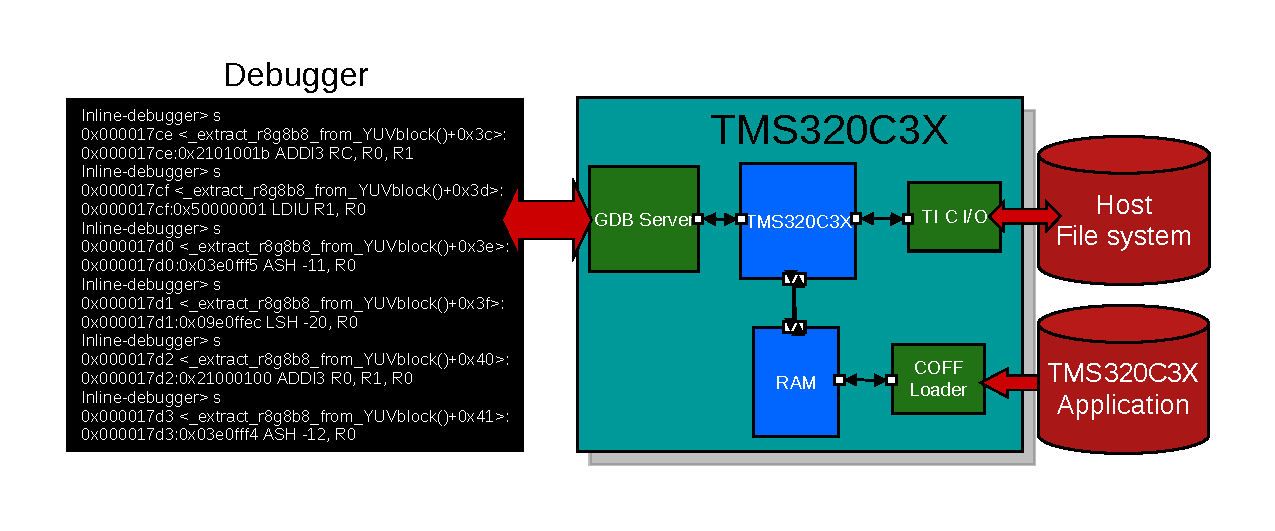
\includegraphics[width=\textwidth]{tms320c3x/fig_tms320c3x.pdf}
	\end{center}
	\caption{TMS320C3X simplified schematic.}
	\label{fig:tms320c3x}
\end{figure}

\subsection{Status of implementation}

The UNISIM TMS320C3X has been developed using the following documentation:
\begin{itemize}
\item TMS320C3x User’s Guide (SPRU031F, 2558539-9761 revision L, March 2004)
\item TMS320C3x/C4x Assembly Language Tools User’s Guide (SPRU035D, June 1998)
\item TMS320C3x/C4x Optimizing C Compiler User’s Guide (SPRU034H, June 1998)
\end{itemize}

The simulator current implementation completely decodes the TMS320C3X instruction set.
All registers are present but no on-chip devices are implemented.
The simulator has complete support for:
\begin{itemize}
\item integer instructions (2-ops, 3-ops, parallel ops, load/store)
\item floating point instructions (2-ops, 3-ops, parallel ops, load/store)
\item control instructions (branches, delayed branches, RPTS, RPTB), but \texttt{iack} and \texttt{swi} instructions
\item interlocked instructions, but \texttt{sigi} instruction
\item power instructions
\item interrupt handling
\end{itemize}

The current status of the simulator allows to run any integer or floating-point benchmark.
However, during the validation process of the UNISIM TMS320C3X simulator, four hardware bugs have been found on our development board, and one software bug in Code Composer.
The UNISIM TMS320C3X simulator can emulate these bugs (see Section~\ref{tms320c3x_configuration}) if they are enabled:
\begin{itemize}
\item \texttt{LDF || LDF} bug: From our experiments on the development board, uncomprehensibly \texttt{src1} is not correctly transformed to a valid \texttt{0.0} when the \texttt{src1} exponent is \texttt{0x80}. Simulator parameter \texttt{cpu.enable-parallel-load-bug} enables this bug.
\item \texttt{STF || STF} and \texttt{STI || STI} bugs: From our experiments on the development board, the first store is never performed. Simulator parameter \texttt{cpu.enable-parallel-store-bug} enables these bugs.
\item \texttt{RND} bug: TMS320C3x User’s Guide says that the \texttt{rnd} instruction does not affect the \texttt{Z} flag however the real hardware systematically sets \texttt{Z} to 0. Simulator parameter \texttt{cpu.enable-rnd-bug} enables this bug.
\item \texttt{lseek} bug: From our experiments on the development board, function \texttt{lseek} from \texttt{RTS30.LIB} has a 32-bit return value truncated to 16 bits. Simulator parameter \texttt{ti-c-io.enable-lseek-bug} enables this bug.
\item floating point instructions bug: All the float instructions can use non-extended registers (all the registers different than \texttt{R0-R7}). However their behavior when using non-extended registers is not documented, and from our experiments on the development board their behavior is unexpected. By default, the simulator does not allow the use of non-extended registers for float instructions (obviously with the exception of the \texttt{FIX} and \texttt{FLOAT} instructions when the use of non-extended registers is documented). Simulator parameter \texttt{cpu.enable-float-ops-with-non-ext-regs} allows the use of non-extended registers for float instructions. Note that the behavior of the instructions when using non-extended registers has been deduced from our experiments with the evaluation board, but that they can not be validated due to the lack of documentation and unexpected behavior.
\end{itemize}

\subsection{Compiling the simulator}

Up-to-date instructions for compiling the simulator are available in the \texttt{INSTALL} file.

\subsection{Invoking the simulator}

The general command line format for invoking the simulator is the following:

\begin{verbatim}
unisim-tms320c3x-2.0 [<options>] <binary to simulate>
\end{verbatim}

\noindent The binary to simulate must be a TI's COFF v0, v1 or v2 file. See~\ref{tms320c3x_cross_compiler} to generate such files.
\newline\\
\noindent The command line options of the simulator are:

\begin{itemize}
\item \texttt{--set $<$param=value$>$ or -s $<$param=value$>$}: set value of parameter 'param' to 'value'
\item \texttt{--config $<$XML file$>$ or -c $<$XML file$>$}: configures the simulator with the given XML configuration file
\item \texttt{--get-config $<$XML file$>$ or -g $<$XML file$>$}: get the simulator configuration XML file (you can use it to create your own configuration. This option can be combined with -c to get a new configuration file with existing variables from another file
\item \texttt{--list or -l}: lists all available parameters, their type, and their current value
\item \texttt{--warn or -w}: enable printing of kernel warnings
\item \texttt{--doc $<$Latex file$>$ or -d $<$Latex file$>$}: enable printing a latex documentation
\item \texttt{--version or -v}: displays the program version information
\item \texttt{--share-path $<$path$>$ or -p $<$path$>$}: the path that should be used for the share directory (absolute path)
\item \texttt{--help or -h}: displays this help
\end{itemize}

\subsection{The Texas Instrument cross-compiler for TMS320C3X}
\label{tms320c3x_cross_compiler}

To compile programs for the TMS320C3X simulator, you can use the free evaluation cross-compiler for TMS320C3X running on a Windows host (SPRC147, TMS320C3x DSK Software) available at \url{http://focus.ti.com/docs/toolsw/folders/print/tmdsdsk33.html}.
This cross-compiler also runs under other x86 operating systems such as Linux or MacOSX using Wine, a Windows emulator (\url{http://www.winehq.org/}).

\textit{Note: Be aware that any call to the C standard library requires linking the program with \texttt{RTS30.LIB}.
Moreover, any call to I/O functions (open, close, read, write, printf, \ldots) requires TI C I/O support enabled in the TMS320C3X simulator.}

The cross-compiler tool chain (\texttt{CL30.EXE, LNK30.EXE, ASM30.EXE, MK30.EXE, ar30.EXE, \ldots}) should be in your \texttt{PATH}.
The shell variable \texttt{C\_DIR} points to the location where the cross-compiler should search for the standard C headers and libraries.
Suppose the tool chain is installed in \texttt{C:{\textbackslash}TI}.
Windows users should add the following in their \texttt{AUTOEXEC.BAT}:
\begin{verbatim}
set PATH=C:\TI\TIC3X4X\BIN;%PATH%
set C_DIR=C:\TI\TIC3X4X\INCLUDE;C:\TI\TIC3X4X\LIB
\end{verbatim}
Wine and GNU bash users should add the following in their \texttt{.bashrc}:
\begin{verbatim}
export PATH=${HOME}/.wine/drive_c/TI/TIC3X4X/BIN:${PATH}
export C_DIR=C:\\TI\\TIC3X4X\\INCLUDE\;C:\\TI\\TIC3X4X\\LIB
\end{verbatim}

\subsection{The GNU binutils}

The GNU binutils are a set of open source tools to manipulate binaries. They provide an assembler, a linker, and an object dump utility among others.
The last version, at the time of writing this document, is available at: \url{ftp://ftp.gnu.org/gnu/binutils/binutils-2.19.1.tar.gz}
The GNU binutils support TI COFF v0, v1 and v2 binary files for both TMS320C3X and TMS320C4X targets.

To compile the binutils and install them into \texttt{/opt/c4x-coff}:

\begin{verbatim}
$ ./configure --target=c4x-unknown-coff --prefix=/opt/c4x-coff
$ make
$ make install
\end{verbatim}

A key feature of the GNU binutils is the ability of \texttt{objdump} to dump/disassemble a TI COFF binary for the TMS320C3X.
For instance, the following command will dump file \texttt{test.out} into file \texttt{dump.txt}:

\begin{verbatim}
$ /opt/c4x-coff/bin/c4x-unknown-coff-objdump -D test.out > dump.txt
\end{verbatim}

\subsection{The GNU GDB debugger}

Version 4.16 of GDB was patched to support C3x/C4x (see \url{http://www.elec.canterbury.ac.nz/c4x/doc/c4x-tools.html} and \url{ftp://ftp.rtems.com/pub/c4x-tools}).
We've slightly patched again this port to make it work on a modern Linux distribution.
It runs on 32-bit x86 Linux hosts.
It is available at: \url{http://unisim-vp.org/site/downloads/other/crosstool/c4x-coff-gdb-4.16.tar.gz}.

To build this special version of GDB, do the following commands:
\begin{verbatim}
$ tar x c4x-coff-gdb-4.16.tar.gz
$ cd c4x-coff-gdb-4.16
$ ./build.sh all
\end{verbatim}

That special GDB can connects to the UNISIM TMS320C3X simulator:

\begin{verbatim}
$ unisim-tms320c3x-2.0 -s enable-gdb-server=true -s gdb-server.tcp-port=1234
\end{verbatim}

\begin{verbatim}
$ ./c4-coff-gdb/bin/c4-coff-gdb 
(gdb) set machine 30
(gdb) target remote localhost:1234
\end{verbatim}

\subsection{Simulator configuration}
\label{tms320c3x_configuration}

\noindent The simulator stores its configuration (a set of parameters) in a XML configuration file. 
\newline\\
\noindent The simulator can provide the user with a default XML configuration file with option \texttt{-g}:

\begin{verbatim}
$ unisim-tms320c3x-2.0 -g default_sim_config.xml
\end{verbatim}

\noindent The simulator can load a XML configuration file with option \texttt{-c}:

\begin{verbatim}
$ unisim-tms320c3x-2.0 -c sim_config.xml
\end{verbatim}

\noindent \textit{Note: Although it's not strictly necessary, parameter \texttt{inline-debugger.memory-atom-size} should be set to value 4 as the TMS320C3X memory is not byte-addressable. If this parameter is not set to 4, presentation of the memory content and disassembly may seem unconventional in the inline debugger.}

\noindent The available parameters are summarized in table below:

\begin{center}
\tablehead{\hline}
\tabletail{\hline}
\begin{supertabular}{|p{7.5cm}|p{7.5cm}|}
	\multicolumn{2}{|l|}{\textbf{\Large Global}}\\
	\hline
	\multicolumn{1}{|p{7.5cm}}{\textbf{Name:} \texttt{enable-gdb-server}} & \multicolumn{1}{p{7.5cm}|}{\textbf{Type:} \texttt{parameter}}\\
	\multicolumn{1}{|p{7.5cm}}{\textbf{Default:} \texttt{false}} & \multicolumn{1}{p{7.5cm}|}{\textbf{Data type:} \texttt{boolean}}\\
	\multicolumn{2}{|p{15cm}|}{\textbf{Valid:} \texttt{true},~\texttt{false}}\\
	\multicolumn{2}{|l|}{}\\
	\multicolumn{2}{|p{15cm}|}{\textbf{Description:} \newline Enable/Disable GDB server instantiation.}\\
	\hline
	\multicolumn{1}{|p{7.5cm}}{\textbf{Name:} \texttt{enable-inline-debugger}} & \multicolumn{1}{p{7.5cm}|}{\textbf{Type:} \texttt{parameter}}\\
	\multicolumn{1}{|p{7.5cm}}{\textbf{Default:} \texttt{false}} & \multicolumn{1}{p{7.5cm}|}{\textbf{Data type:} \texttt{boolean}}\\
	\multicolumn{2}{|p{15cm}|}{\textbf{Valid:} \texttt{true},~\texttt{false}}\\
	\multicolumn{2}{|l|}{}\\
	\multicolumn{2}{|p{15cm}|}{\textbf{Description:} \newline Enable/Disable inline debugger instantiation.}\\
	\hline
	\multicolumn{1}{|p{7.5cm}}{\textbf{Name:} \texttt{enable-press-enter-at-exit}} & \multicolumn{1}{p{7.5cm}|}{\textbf{Type:} \texttt{parameter}}\\
	\multicolumn{1}{|p{7.5cm}}{\textbf{Default:} \texttt{false}} & \multicolumn{1}{p{7.5cm}|}{\textbf{Data type:} \texttt{boolean}}\\
	\multicolumn{2}{|p{15cm}|}{\textbf{Valid:} \texttt{true},~\texttt{false}}\\
	\multicolumn{2}{|l|}{}\\
	\multicolumn{2}{|p{15cm}|}{\textbf{Description:} \newline Enable/Disable pressing key enter at exit.}\\
	\hline
	\multicolumn{1}{|p{7.5cm}}{\textbf{Name:} \texttt{kernel\_logger.file}} & \multicolumn{1}{p{7.5cm}|}{\textbf{Type:} \texttt{parameter}}\\
	\multicolumn{1}{|p{7.5cm}}{\textbf{Default:} \texttt{false}} & \multicolumn{1}{p{7.5cm}|}{\textbf{Data type:} \texttt{boolean}}\\
	\multicolumn{2}{|p{15cm}|}{\textbf{Valid:} \texttt{true},~\texttt{false}}\\
	\multicolumn{2}{|l|}{}\\
	\multicolumn{2}{|p{15cm}|}{\textbf{Description:} \newline Keep logger output in a file.}\\
	\hline
	\multicolumn{1}{|p{7.5cm}}{\textbf{Name:} \texttt{kernel\_logger.filename}} & \multicolumn{1}{p{7.5cm}|}{\textbf{Type:} \texttt{parameter}}\\
	\multicolumn{1}{|p{7.5cm}}{\textbf{Default:} \texttt{logger\_output.txt}} & \multicolumn{1}{p{7.5cm}|}{\textbf{Data type:} \texttt{string}}\\
	\multicolumn{2}{|l|}{}\\
	\multicolumn{2}{|l|}{}\\
	\multicolumn{2}{|p{15cm}|}{\textbf{Description:} \newline Filename to keep logger output (the option file must be activated).}\\
	\hline
	\multicolumn{1}{|p{7.5cm}}{\textbf{Name:} \texttt{kernel\_logger.std\_err}} & \multicolumn{1}{p{7.5cm}|}{\textbf{Type:} \texttt{parameter}}\\
	\multicolumn{1}{|p{7.5cm}}{\textbf{Default:} \texttt{true}} & \multicolumn{1}{p{7.5cm}|}{\textbf{Data type:} \texttt{boolean}}\\
	\multicolumn{2}{|p{15cm}|}{\textbf{Valid:} \texttt{true},~\texttt{false}}\\
	\multicolumn{2}{|l|}{}\\
	\multicolumn{2}{|p{15cm}|}{\textbf{Description:} \newline Show logger output through the standard error output.}\\
	\hline
	\multicolumn{1}{|p{7.5cm}}{\textbf{Name:} \texttt{kernel\_logger.std\_err\_color}} & \multicolumn{1}{p{7.5cm}|}{\textbf{Type:} \texttt{parameter}}\\
	\multicolumn{1}{|p{7.5cm}}{\textbf{Default:} \texttt{false}} & \multicolumn{1}{p{7.5cm}|}{\textbf{Data type:} \texttt{boolean}}\\
	\multicolumn{2}{|p{15cm}|}{\textbf{Valid:} \texttt{true},~\texttt{false}}\\
	\multicolumn{2}{|l|}{}\\
	\multicolumn{2}{|p{15cm}|}{\textbf{Description:} \newline Colorize logger output through the standard error output (only works if std\_err is active).}\\
	\hline
	\multicolumn{1}{|p{7.5cm}}{\textbf{Name:} \texttt{kernel\_logger.std\_out}} & \multicolumn{1}{p{7.5cm}|}{\textbf{Type:} \texttt{parameter}}\\
	\multicolumn{1}{|p{7.5cm}}{\textbf{Default:} \texttt{false}} & \multicolumn{1}{p{7.5cm}|}{\textbf{Data type:} \texttt{boolean}}\\
	\multicolumn{2}{|p{15cm}|}{\textbf{Valid:} \texttt{true},~\texttt{false}}\\
	\multicolumn{2}{|l|}{}\\
	\multicolumn{2}{|p{15cm}|}{\textbf{Description:} \newline Show logger output through the standard output.}\\
	\hline
	\multicolumn{1}{|p{7.5cm}}{\textbf{Name:} \texttt{kernel\_logger.std\_out\_color}} & \multicolumn{1}{p{7.5cm}|}{\textbf{Type:} \texttt{parameter}}\\
	\multicolumn{1}{|p{7.5cm}}{\textbf{Default:} \texttt{false}} & \multicolumn{1}{p{7.5cm}|}{\textbf{Data type:} \texttt{boolean}}\\
	\multicolumn{2}{|p{15cm}|}{\textbf{Valid:} \texttt{true},~\texttt{false}}\\
	\multicolumn{2}{|l|}{}\\
	\multicolumn{2}{|p{15cm}|}{\textbf{Description:} \newline Colorize logger output through the standard output (only works if std\_out is active).}\\
	\hline
	\multicolumn{1}{|p{7.5cm}}{\textbf{Name:} \texttt{kernel\_logger.xml\_file}} & \multicolumn{1}{p{7.5cm}|}{\textbf{Type:} \texttt{parameter}}\\
	\multicolumn{1}{|p{7.5cm}}{\textbf{Default:} \texttt{false}} & \multicolumn{1}{p{7.5cm}|}{\textbf{Data type:} \texttt{boolean}}\\
	\multicolumn{2}{|p{15cm}|}{\textbf{Valid:} \texttt{true},~\texttt{false}}\\
	\multicolumn{2}{|l|}{}\\
	\multicolumn{2}{|p{15cm}|}{\textbf{Description:} \newline Keep logger output in a file xml formatted.}\\
	\hline
	\multicolumn{1}{|p{7.5cm}}{\textbf{Name:} \texttt{kernel\_logger.xml\_file\_gzipped}} & \multicolumn{1}{p{7.5cm}|}{\textbf{Type:} \texttt{parameter}}\\
	\multicolumn{1}{|p{7.5cm}}{\textbf{Default:} \texttt{false}} & \multicolumn{1}{p{7.5cm}|}{\textbf{Data type:} \texttt{boolean}}\\
	\multicolumn{2}{|p{15cm}|}{\textbf{Valid:} \texttt{true},~\texttt{false}}\\
	\multicolumn{2}{|l|}{}\\
	\multicolumn{2}{|p{15cm}|}{\textbf{Description:} \newline If the xml\_file option is active, the output file will be compressed (a .gz extension will be automatically added to the xml\_filename option.}\\
	\hline
	\multicolumn{1}{|p{7.5cm}}{\textbf{Name:} \texttt{kernel\_logger.xml\_filename}} & \multicolumn{1}{p{7.5cm}|}{\textbf{Type:} \texttt{parameter}}\\
	\multicolumn{1}{|p{7.5cm}}{\textbf{Default:} \texttt{logger\_output.xml}} & \multicolumn{1}{p{7.5cm}|}{\textbf{Data type:} \texttt{string}}\\
	\multicolumn{2}{|l|}{}\\
	\multicolumn{2}{|l|}{}\\
	\multicolumn{2}{|p{15cm}|}{\textbf{Description:} \newline Filename to keep logger xml output (the option xml\_file must be activated).}\\
	\hline
	\hline
	\multicolumn{2}{|l|}{\textbf{\Large cpu}}\\
	\hline
	\multicolumn{1}{|p{7.5cm}}{\textbf{Name:} \texttt{cpu.max-inst}} & \multicolumn{1}{p{7.5cm}|}{\textbf{Type:} \texttt{parameter}}\\
	\multicolumn{1}{|p{7.5cm}}{\textbf{Default:} \texttt{0xffffffffffffffff}} & \multicolumn{1}{p{7.5cm}|}{\textbf{Data type:} \texttt{unsigned 64-bit integer}}\\
	\multicolumn{2}{|l|}{}\\
	\hline
	\multicolumn{1}{|p{7.5cm}}{\textbf{Name:} \texttt{cpu.trap-on-instruction-counter}} & \multicolumn{1}{p{7.5cm}|}{\textbf{Type:} \texttt{parameter}}\\
	\multicolumn{1}{|p{7.5cm}}{\textbf{Default:} \texttt{0xffffffffffffffff}} & \multicolumn{1}{p{7.5cm}|}{\textbf{Data type:} \texttt{unsigned 64-bit integer}}\\
	\multicolumn{2}{|l|}{}\\
	\hline
	\multicolumn{1}{|p{7.5cm}}{\textbf{Name:} \texttt{cpu.mimic-dev-board}} & \multicolumn{1}{p{7.5cm}|}{\textbf{Type:} \texttt{parameter}}\\
	\multicolumn{1}{|p{7.5cm}}{\textbf{Default:} \texttt{true}} & \multicolumn{1}{p{7.5cm}|}{\textbf{Data type:} \texttt{boolean}}\\
	\multicolumn{2}{|p{15cm}|}{\textbf{Valid:} \texttt{true},~\texttt{false}}\\
	\hline
	\multicolumn{1}{|p{7.5cm}}{\textbf{Name:} \texttt{cpu.enable-parallel-load-bug}} & \multicolumn{1}{p{7.5cm}|}{\textbf{Type:} \texttt{parameter}}\\
	\multicolumn{1}{|p{7.5cm}}{\textbf{Default:} \texttt{true}} & \multicolumn{1}{p{7.5cm}|}{\textbf{Data type:} \texttt{boolean}}\\
	\multicolumn{2}{|p{15cm}|}{\textbf{Valid:} \texttt{true},~\texttt{false}}\\
	\multicolumn{2}{|l|}{}\\
	\multicolumn{2}{|p{15cm}|}{\textbf{Description:} \newline When using parallel loads (LDF src2, dst2 || LDF src1, dst1) the src1 load doesn't transform incorrect zero values to valid zero representation, instead they copy the contents of the memory to the register. Set to this parameter to false to transform incorrect zero values..}\\
	\hline
	\multicolumn{1}{|p{7.5cm}}{\textbf{Name:} \texttt{cpu.enable-rnd-bug}} & \multicolumn{1}{p{7.5cm}|}{\textbf{Type:} \texttt{parameter}}\\
	\multicolumn{1}{|p{7.5cm}}{\textbf{Default:} \texttt{true}} & \multicolumn{1}{p{7.5cm}|}{\textbf{Data type:} \texttt{boolean}}\\
	\multicolumn{2}{|p{15cm}|}{\textbf{Valid:} \texttt{true},~\texttt{false}}\\
	\multicolumn{2}{|l|}{}\\
	\multicolumn{2}{|p{15cm}|}{\textbf{Description:} \newline If enabled the `rnd` instruction sets the Z flag to 0 systematically, as it is done in the evaluation board. Otherwise, Z is unchanged as it is written in the documentation..}\\
	\hline
	\multicolumn{1}{|p{7.5cm}}{\textbf{Name:} \texttt{cpu.enable-parallel-store-} \newline$\hookrightarrow$\texttt{bug}} & \multicolumn{1}{p{7.5cm}|}{\textbf{Type:} \texttt{parameter}}\\
	\multicolumn{1}{|p{7.5cm}}{\textbf{Default:} \texttt{true}} & \multicolumn{1}{p{7.5cm}|}{\textbf{Data type:} \texttt{boolean}}\\
	\multicolumn{2}{|p{15cm}|}{\textbf{Valid:} \texttt{true},~\texttt{false}}\\
	\multicolumn{2}{|l|}{}\\
	\multicolumn{2}{|p{15cm}|}{\textbf{Description:} \newline If enabled, when using parallel stores (STF src2, dst2 || STF src1, dst1) the first store is treated as a NOP..}\\
	\hline
	\multicolumn{1}{|p{7.5cm}}{\textbf{Name:} \texttt{cpu.enable-float-ops-with-} \newline$\hookrightarrow$\texttt{non-ext-regs}} & \multicolumn{1}{p{7.5cm}|}{\textbf{Type:} \texttt{parameter}}\\
	\multicolumn{1}{|p{7.5cm}}{\textbf{Default:} \texttt{false}} & \multicolumn{1}{p{7.5cm}|}{\textbf{Data type:} \texttt{boolean}}\\
	\multicolumn{2}{|p{15cm}|}{\textbf{Valid:} \texttt{true},~\texttt{false}}\\
	\multicolumn{2}{|l|}{}\\
	\multicolumn{2}{|p{15cm}|}{\textbf{Description:} \newline If enabled non extended registers can be used on all the float instructions, however the behavior is not documented and can differ between chips revision. If disabled, it stops simulation when using non extended registers on float instructions..}\\
	\hline
	\multicolumn{1}{|p{7.5cm}}{\textbf{Name:} \texttt{cpu.verbose-all}} & \multicolumn{1}{p{7.5cm}|}{\textbf{Type:} \texttt{parameter}}\\
	\multicolumn{1}{|p{7.5cm}}{\textbf{Default:} \texttt{false}} & \multicolumn{1}{p{7.5cm}|}{\textbf{Data type:} \texttt{boolean}}\\
	\multicolumn{2}{|p{15cm}|}{\textbf{Valid:} \texttt{true},~\texttt{false}}\\
	\hline
	\multicolumn{1}{|p{7.5cm}}{\textbf{Name:} \texttt{cpu.verbose-setup}} & \multicolumn{1}{p{7.5cm}|}{\textbf{Type:} \texttt{parameter}}\\
	\multicolumn{1}{|p{7.5cm}}{\textbf{Default:} \texttt{false}} & \multicolumn{1}{p{7.5cm}|}{\textbf{Data type:} \texttt{boolean}}\\
	\multicolumn{2}{|p{15cm}|}{\textbf{Valid:} \texttt{true},~\texttt{false}}\\
	\hline
	\hline
	\multicolumn{2}{|l|}{\textbf{\Large loader}}\\
	\hline
	\multicolumn{1}{|p{7.5cm}}{\textbf{Name:} \texttt{loader.verbose}} & \multicolumn{1}{p{7.5cm}|}{\textbf{Type:} \texttt{parameter}}\\
	\multicolumn{1}{|p{7.5cm}}{\textbf{Default:} \texttt{false}} & \multicolumn{1}{p{7.5cm}|}{\textbf{Data type:} \texttt{boolean}}\\
	\multicolumn{2}{|p{15cm}|}{\textbf{Valid:} \texttt{true},~\texttt{false}}\\
	\multicolumn{2}{|l|}{}\\
	\multicolumn{2}{|p{15cm}|}{\textbf{Description:} \newline Enable/Disable verbosity.}\\
	\hline
	\multicolumn{1}{|p{7.5cm}}{\textbf{Name:} \texttt{loader.verbose-parser}} & \multicolumn{1}{p{7.5cm}|}{\textbf{Type:} \texttt{parameter}}\\
	\multicolumn{1}{|p{7.5cm}}{\textbf{Default:} \texttt{false}} & \multicolumn{1}{p{7.5cm}|}{\textbf{Data type:} \texttt{boolean}}\\
	\multicolumn{2}{|p{15cm}|}{\textbf{Valid:} \texttt{true},~\texttt{false}}\\
	\multicolumn{2}{|l|}{}\\
	\multicolumn{2}{|p{15cm}|}{\textbf{Description:} \newline Enable/Disable verbosity of parser.}\\
	\hline
	\multicolumn{1}{|p{7.5cm}}{\textbf{Name:} \texttt{loader.filename}} & \multicolumn{1}{p{7.5cm}|}{\textbf{Type:} \texttt{parameter}}\\
	\multicolumn{1}{|p{7.5cm}}{\textbf{Default:} \texttt{c31boot.out}} & \multicolumn{1}{p{7.5cm}|}{\textbf{Data type:} \texttt{string}}\\
	\multicolumn{2}{|l|}{}\\
	\multicolumn{2}{|l|}{}\\
	\multicolumn{2}{|p{15cm}|}{\textbf{Description:} \newline List of files to load. Syntax: [[filename=]$<$filename1$>$[:[format=]$<$format1$>$]][,[filename=]$<$filename2$>$[:[format=]$<$format2$>$]]... (e.g. boot.bin:raw,app.elf).}\\
	\hline
	\hline
	\multicolumn{2}{|l|}{\textbf{\Large loader.memory-mapper}}\\
	\hline
	\multicolumn{1}{|p{7.5cm}}{\textbf{Name:} \texttt{loader.memory-mapper.verbose}} & \multicolumn{1}{p{7.5cm}|}{\textbf{Type:} \texttt{parameter}}\\
	\multicolumn{1}{|p{7.5cm}}{\textbf{Default:} \texttt{false}} & \multicolumn{1}{p{7.5cm}|}{\textbf{Data type:} \texttt{boolean}}\\
	\multicolumn{2}{|p{15cm}|}{\textbf{Valid:} \texttt{true},~\texttt{false}}\\
	\multicolumn{2}{|l|}{}\\
	\multicolumn{2}{|p{15cm}|}{\textbf{Description:} \newline Enable/Disable verbosity.}\\
	\hline
	\multicolumn{1}{|p{7.5cm}}{\textbf{Name:} \texttt{loader.memory-mapper.verbose-} \newline$\hookrightarrow$\texttt{parser}} & \multicolumn{1}{p{7.5cm}|}{\textbf{Type:} \texttt{parameter}}\\
	\multicolumn{1}{|p{7.5cm}}{\textbf{Default:} \texttt{false}} & \multicolumn{1}{p{7.5cm}|}{\textbf{Data type:} \texttt{boolean}}\\
	\multicolumn{2}{|p{15cm}|}{\textbf{Valid:} \texttt{true},~\texttt{false}}\\
	\multicolumn{2}{|l|}{}\\
	\multicolumn{2}{|p{15cm}|}{\textbf{Description:} \newline Enable/Disable verbosity of parser.}\\
	\hline
	\multicolumn{1}{|p{7.5cm}}{\textbf{Name:} \texttt{loader.memory-mapper.mapping}} & \multicolumn{1}{p{7.5cm}|}{\textbf{Type:} \texttt{parameter}}\\
	\multicolumn{1}{|p{7.5cm}}{\textbf{Default:} \texttt{memory=memory:0x0-0xffffffff}} & \multicolumn{1}{p{7.5cm}|}{\textbf{Data type:} \texttt{string}}\\
	\multicolumn{2}{|l|}{}\\
	\multicolumn{2}{|l|}{}\\
	\multicolumn{2}{|p{15cm}|}{\textbf{Description:} \newline Memory mapping. Syntax: [[(memory=]$<$memory1$>$[:[range=]$<$low1-high1$>$]][,[(memory=]$<$memory2$>$[:[range=]$<$low2-high2$>$]]... (e.g. ram:0x0-0x00ffff,rom:0xff0000-0xffffff).}\\
	\hline
	\hline
	\multicolumn{2}{|l|}{\textbf{\Large memory}}\\
	\hline
	\multicolumn{1}{|p{7.5cm}}{\textbf{Name:} \texttt{memory.org}} & \multicolumn{1}{p{7.5cm}|}{\textbf{Type:} \texttt{parameter}}\\
	\multicolumn{1}{|p{7.5cm}}{\textbf{Default:} \texttt{0x0000000000000000}} & \multicolumn{1}{p{7.5cm}|}{\textbf{Data type:} \texttt{unsigned 64-bit integer}}\\
	\multicolumn{2}{|l|}{}\\
	\multicolumn{2}{|l|}{}\\
	\multicolumn{2}{|p{15cm}|}{\textbf{Description:} \newline memory origin/base address.}\\
	\hline
	\multicolumn{1}{|p{7.5cm}}{\textbf{Name:} \texttt{memory.bytesize}} & \multicolumn{1}{p{7.5cm}|}{\textbf{Type:} \texttt{parameter}}\\
	\multicolumn{1}{|p{7.5cm}}{\textbf{Default:} \texttt{0}} & \multicolumn{1}{p{7.5cm}|}{\textbf{Data type:} \texttt{unsigned 64-bit integer}}\\
	\multicolumn{2}{|l|}{}\\
	\multicolumn{2}{|l|}{}\\
	\multicolumn{2}{|p{15cm}|}{\textbf{Description:} \newline memory size in bytes.}\\
	\hline
	\hline
	\multicolumn{2}{|l|}{\textbf{\Large ti-c-io}}\\
	\hline
	\multicolumn{1}{|p{7.5cm}}{\textbf{Name:} \texttt{ti-c-io.enable}} & \multicolumn{1}{p{7.5cm}|}{\textbf{Type:} \texttt{parameter}}\\
	\multicolumn{1}{|p{7.5cm}}{\textbf{Default:} \texttt{true}} & \multicolumn{1}{p{7.5cm}|}{\textbf{Data type:} \texttt{boolean}}\\
	\multicolumn{2}{|p{15cm}|}{\textbf{Valid:} \texttt{true},~\texttt{false}}\\
	\multicolumn{2}{|l|}{}\\
	\multicolumn{2}{|p{15cm}|}{\textbf{Description:} \newline enable/disable TI C I/O support.}\\
	\hline
	\multicolumn{1}{|p{7.5cm}}{\textbf{Name:} \texttt{ti-c-io.warning-as-error}} & \multicolumn{1}{p{7.5cm}|}{\textbf{Type:} \texttt{parameter}}\\
	\multicolumn{1}{|p{7.5cm}}{\textbf{Default:} \texttt{false}} & \multicolumn{1}{p{7.5cm}|}{\textbf{Data type:} \texttt{boolean}}\\
	\multicolumn{2}{|p{15cm}|}{\textbf{Valid:} \texttt{true},~\texttt{false}}\\
	\multicolumn{2}{|l|}{}\\
	\multicolumn{2}{|p{15cm}|}{\textbf{Description:} \newline Whether Warnings are considered as error or not.}\\
	\hline
	\multicolumn{1}{|p{7.5cm}}{\textbf{Name:} \texttt{ti-c-io.pc-register-name}} & \multicolumn{1}{p{7.5cm}|}{\textbf{Type:} \texttt{parameter}}\\
	\multicolumn{1}{|p{7.5cm}}{\textbf{Default:} \texttt{PC}} & \multicolumn{1}{p{7.5cm}|}{\textbf{Data type:} \texttt{string}}\\
	\multicolumn{2}{|l|}{}\\
	\multicolumn{2}{|l|}{}\\
	\multicolumn{2}{|p{15cm}|}{\textbf{Description:} \newline Name of the CPU program counter register.}\\
	\hline
	\multicolumn{1}{|p{7.5cm}}{\textbf{Name:} \texttt{ti-c-io.c-io-buffer-symbol-} \newline$\hookrightarrow$\texttt{name}} & \multicolumn{1}{p{7.5cm}|}{\textbf{Type:} \texttt{parameter}}\\
	\multicolumn{1}{|p{7.5cm}}{\textbf{Default:} \texttt{\_\_CIOBUF\_}} & \multicolumn{1}{p{7.5cm}|}{\textbf{Data type:} \texttt{string}}\\
	\multicolumn{2}{|l|}{}\\
	\multicolumn{2}{|l|}{}\\
	\multicolumn{2}{|p{15cm}|}{\textbf{Description:} \newline C I/O buffer symbol name.}\\
	\hline
	\multicolumn{1}{|p{7.5cm}}{\textbf{Name:} \texttt{ti-c-io.c-io-breakpoint-symbol-} \newline$\hookrightarrow$\texttt{name}} & \multicolumn{1}{p{7.5cm}|}{\textbf{Type:} \texttt{parameter}}\\
	\multicolumn{1}{|p{7.5cm}}{\textbf{Default:} \texttt{C\$\$IO\$\$}} & \multicolumn{1}{p{7.5cm}|}{\textbf{Data type:} \texttt{string}}\\
	\multicolumn{2}{|l|}{}\\
	\multicolumn{2}{|l|}{}\\
	\multicolumn{2}{|p{15cm}|}{\textbf{Description:} \newline C I/O breakpoint symbol name.}\\
	\hline
	\multicolumn{1}{|p{7.5cm}}{\textbf{Name:} \texttt{ti-c-io.c-exit-breakpoint-} \newline$\hookrightarrow$\texttt{symbol-name}} & \multicolumn{1}{p{7.5cm}|}{\textbf{Type:} \texttt{parameter}}\\
	\multicolumn{1}{|p{7.5cm}}{\textbf{Default:} \texttt{C\$\$EXIT}} & \multicolumn{1}{p{7.5cm}|}{\textbf{Data type:} \texttt{string}}\\
	\multicolumn{2}{|l|}{}\\
	\multicolumn{2}{|l|}{}\\
	\multicolumn{2}{|p{15cm}|}{\textbf{Description:} \newline C EXIT breakpoint symbol name.}\\
	\hline
	\multicolumn{1}{|p{7.5cm}}{\textbf{Name:} \texttt{ti-c-io.verbose-all}} & \multicolumn{1}{p{7.5cm}|}{\textbf{Type:} \texttt{parameter}}\\
	\multicolumn{1}{|p{7.5cm}}{\textbf{Default:} \texttt{false}} & \multicolumn{1}{p{7.5cm}|}{\textbf{Data type:} \texttt{boolean}}\\
	\multicolumn{2}{|p{15cm}|}{\textbf{Valid:} \texttt{true},~\texttt{false}}\\
	\multicolumn{2}{|l|}{}\\
	\multicolumn{2}{|p{15cm}|}{\textbf{Description:} \newline globally enable/disable verbosity.}\\
	\hline
	\multicolumn{1}{|p{7.5cm}}{\textbf{Name:} \texttt{ti-c-io.verbose-io}} & \multicolumn{1}{p{7.5cm}|}{\textbf{Type:} \texttt{parameter}}\\
	\multicolumn{1}{|p{7.5cm}}{\textbf{Default:} \texttt{false}} & \multicolumn{1}{p{7.5cm}|}{\textbf{Data type:} \texttt{boolean}}\\
	\multicolumn{2}{|p{15cm}|}{\textbf{Valid:} \texttt{true},~\texttt{false}}\\
	\multicolumn{2}{|l|}{}\\
	\multicolumn{2}{|p{15cm}|}{\textbf{Description:} \newline enable/disable verbosity while I/Os.}\\
	\hline
	\multicolumn{1}{|p{7.5cm}}{\textbf{Name:} \texttt{ti-c-io.verbose-setup}} & \multicolumn{1}{p{7.5cm}|}{\textbf{Type:} \texttt{parameter}}\\
	\multicolumn{1}{|p{7.5cm}}{\textbf{Default:} \texttt{false}} & \multicolumn{1}{p{7.5cm}|}{\textbf{Data type:} \texttt{boolean}}\\
	\multicolumn{2}{|p{15cm}|}{\textbf{Valid:} \texttt{true},~\texttt{false}}\\
	\multicolumn{2}{|l|}{}\\
	\multicolumn{2}{|p{15cm}|}{\textbf{Description:} \newline enable/disable verbosity while setup.}\\
	\hline
	\multicolumn{1}{|p{7.5cm}}{\textbf{Name:} \texttt{ti-c-io.enable-lseek-bug}} & \multicolumn{1}{p{7.5cm}|}{\textbf{Type:} \texttt{parameter}}\\
	\multicolumn{1}{|p{7.5cm}}{\textbf{Default:} \texttt{false}} & \multicolumn{1}{p{7.5cm}|}{\textbf{Data type:} \texttt{boolean}}\\
	\multicolumn{2}{|p{15cm}|}{\textbf{Valid:} \texttt{true},~\texttt{false}}\\
	\multicolumn{2}{|l|}{}\\
	\multicolumn{2}{|p{15cm}|}{\textbf{Description:} \newline enable/disable lseek bug (as code composer).}\\
	\hline
	\hline
	\end{supertabular}
\end{center}

\subsection{Debugging the target program}
\label{tms320c3x_inline_debug}

The command line option \texttt{-s enable-inline-debugger=true} enables the inline debugger. The inline debugger has support for controlling the program execution, inspecting the program and its data, and putting breakpoints and watchpoints. The user can interact with the debugger using the following commands:
\begin{itemize}
\item Execution commands:
	\begin{itemize}
	\item \texttt{<c | cont | continue> [<symbol | *address>]}: \newline
	Continue to execute instructions until program reaches a breakpoint, a watchpoint, a `symbol' or an `address'.
	\item \texttt{<s | si | step | stepi>}: \newline
	Execute one instruction.
	\item \texttt{<n | ni | next | nexti>}: \newline
	Continue to execute instructions until the processor reaches next contiguous instruction, a breakpoint or a watchpoint.
	\item \texttt{<r | run>}: \newline
	Restart the simulation from the beginning (not yet supported).
	\end{itemize}
\item Inspection commands:
	\begin{itemize}
	\item \texttt{<dis | disasm | disassemble> [<symbol | *address>]}: \newline
	Continue to disassemble starting from `symbol', `address', or after the previous disassembly.
	\item \texttt{<d | dump> [<symbol | *address>]}: \newline
	Dump memory starting from `symbol', `address', or after the previous dump.
	\item \texttt{<register name>}: \newline
	Display the register value.
	\item \texttt{<m | monitor> [<variable name>]}: \newline
	Display the given simulator variable (displays all variable names if none is given).
	\item \texttt{<p | prof | profile>} \newline
	\texttt{<p | prof | profile> program} \newline
	\texttt{<p | prof | profile> data} \newline
	\texttt{<p | prof | profile> data read} \newline
	\texttt{<p | prof | profile> data write}: \newline
	Display the program/data profile.
	\end{itemize}
\item Breakpoints/Watchpoints commands:
	\begin{itemize}
	\item \texttt{<b | break> [<symbol | *address>]}: \newline
	Set a breakpoint at `symbol' or `address'. If `symbol' or `address' are not specified, display the breakpoint list.
	\item \texttt{<w | watch> [<symbol | *address[:<size>]>] [<read | write>]}: \newline
	Set a watchpoint at `symbol' or `address'. When using `continue' and `next' commands, the debugger will spy CPU loads and stores. The debugger will return to the command line prompt once a load or a store accesses to the given `symbol' or `address'.
	\item \texttt{<del | delete> <symbol | *address>}: \newline
	Delete the breakpoint at `symbol' or `address'.
	\item \texttt{<delw | delwatch> <symbol | *address> [<read | write>] [<size>]}: \newline
	Delete the watchpoint at 'symbol' or 'address'.
	\end{itemize}
\item Miscellaneous commands:
	\begin{itemize}
	\item \texttt{<h | ? | help>}: \newline
	Display the integrated help.
	\item \texttt{<quit | q>}: \newline
	Quit the built-in debugger.
	\end{itemize}
\end{itemize}

\newpage
\section{Developer guide}

The TMS320C3X simulator is the combination of several software components:
\begin{itemize}
\item A unisim core infrastructure in \texttt{unisim/kernel} (see Section~\ref{tms320c3x_service_infrastructure}).
\item A built-in logger in \texttt{unisim/kernel/logger} (see Section~\ref{tms320c3x_logger}).
\item Several small utility classes in \texttt{unisim/util} (see Section~\ref{tms320c3x_utils}).
\item A TMS320C3X instruction set simulator in \texttt{unisim/component/cxx/processor/tms320} (see Section~\ref{tms320c3x_iss}).
\item A memory in \texttt{unisim/component/cxx/memory/ram} (see Section~\ref{tms320c3x_memory}).
\item Service interface definitions in \texttt{unisim/service/interfaces} (see Section~\ref{tms320c3x_interfaces}).
\item A multi-format loader (COFF, ELF, S-Rec, Raw) service and especially a COFF loader in \texttt{unisim/service/loader/coff\_loader} (see Section~\ref{tms320c3x_coff_loader}).
\item A TI C I/O service in \texttt{unisim/service/os/ti\_c\_io} (see Section~\ref{tms320c3x_ti_c_io}).
\item An inline debugger service in \texttt{unisim/service/debug/inline\_debugger} (see Section~\ref{tms320c3x_inline_debugger}).
\item A GDB server service in \texttt{unisim/service/debug/gdb\_server} (see Section~\ref{tms320c3x_gdb_server}).
\end{itemize}

\subsection{Simulation Components}

\subsubsection{TMS320C3X instruction set simulator}
\label{tms320c3x_iss}

The instruction set simulator source code is located in directory: \newline \texttt{unisim/component/cxx/processor/tms320}.\newline
The UNISIM TMS320C3X instruction set simulator uses an instruction set simulator generator, GenISSLib.
GenISSLib uses an instruction set description (\texttt{.isa} files) located in sub-directory \texttt{isa} of the instruction set simulator source code directory.
Most computations (e.g., integer computation) are directly performed in these description files.
See the GenISSLib manual for additional informations about the GenISSLib instruction set description language.
The simulator is implemented in class \texttt{unisim::component::cxx::processor::tms320::CPU}, and its main methods are:
\begin{itemize}
\item \texttt{StepInstruction}: Executes one instruction.
\item \texttt{PrWrite}: Write a word into memory using service import \texttt{memory\_import} (see Section~\ref{tms320c3x_service_infrastructure} for details about services). This method is virtual so that it can be reimplemented into a derived class.
\item \texttt{PrRead}: Read a word from memory using service import \texttt{memory\_import} (see Section~\ref{tms320c3x_service_infrastructure} for details about services). This method is virtual so that it can be reimplemented into a derived class.
\item \texttt{SetIRQLevel}: Set level (0/1, true/false) of an IRQ. IRQ numbering is same as register \texttt{IF} bit numbering.
\item \texttt{ComputeIndirEA}: Compute the effective address for indirect addressing modes.
\item \texttt{ComputeDirEA}: Compute the effective address for direct addressing modes.
\end{itemize}
This class is a client and a service (see Section~\ref{tms320c3x_service_infrastructure} for details) that can be connected to a debugger, a loader, and a memory.

Each register (R0, R1, R2, R3, R4, R5, R6, R7, ar0, ar1, ar2, ar3, ar4, ar5, ar6, ar7, DP, IR0, IR1, BK, SP, ST, IE, IF, IOF, RS, RE, and RC) is implemented by an instance of class \texttt{unisim::component::cxx::processor::tms320::Register}.
This class has methods to get/set value of a register and to perform floating point computations.

\noindent The table below summarizes the API of the CPU:

\begin{center}
	\tablehead{\hline}
	\tabletail{\hline}
	\begin{supertabular}{|p{7.5cm}|p{7.5cm}|}
		\hline
		\multicolumn{2}{|l|}{\textbf{\Large Module CPU}}\\
		\hline
		\multicolumn{1}{|p{7.5cm}}{\textbf{Class Name:} \newline \texttt{unisim::component::cxx::processor}\newline$\hookrightarrow$\texttt{::tms320::CPU}} & \multicolumn{1}{p{7.5cm}|}{\textbf{Header:} \newline \texttt{unisim/component/cxx/processor}\newline$\hookrightarrow$\texttt{/tms320/cpu.hh}}\\
		\multicolumn{2}{|l|}{}\\
		\multicolumn{2}{|p{15cm}|}{\textbf{Description:} \newline This C++ class implements the TMS320C3X instruction set simulator.}\\
		\hline
		\hline
		\multicolumn{2}{|c|}{\textbf{\large Template Parameters}}\\
		\hline
		\multicolumn{1}{|p{7.5cm}}{\textbf{Name:} \texttt{CONFIG}} & \multicolumn{1}{p{7.5cm}|}{\textbf{Type:} \texttt{class}}\\
		\multicolumn{2}{|p{15cm}|}{\textbf{Default value:} \texttt{none}}\\
		\multicolumn{2}{|l|}{}\\
		\multicolumn{2}{|p{15cm}|}{\textbf{Description:} \newline This is a configuration class that is a collection of definitions to parameterize the simulation model.}\\
		\hline
		\multicolumn{1}{|p{7.5cm}}{\textbf{Name:} \texttt{DEBUG}} & \multicolumn{1}{p{7.5cm}|}{\textbf{Type:} \texttt{bool}}\\
		\multicolumn{2}{|p{15cm}|}{\textbf{Default value:} \texttt{false}}\\
		\multicolumn{2}{|l|}{}\\
		\multicolumn{2}{|p{15cm}|}{\textbf{Description:} \newline Enable/disable debug.}\\
		\hline
		\hline
		\multicolumn{2}{|c|}{\textbf{\large Run-Time Parameters}}\\
		\hline
		\multicolumn{1}{|p{7.5cm}}{\textbf{Name:} \texttt{max-inst}} & \multicolumn{1}{p{7.5cm}|}{\textbf{Type:} \texttt{uint64\_t}}\\
		\multicolumn{2}{|p{15cm}|}{\textbf{Default value:} \texttt{$2^{64} - 1$}}\\
		\multicolumn{2}{|l|}{}\\
		\multicolumn{2}{|p{15cm}|}{\textbf{Description:} \newline Maximum number of instructions to simulate. Once this threshold is reached, the CPU calls virtual method \texttt{Stop} to stop simulation.}\\
		\hline
		\multicolumn{1}{|p{7.5cm}}{\textbf{Name:} \texttt{trap-on-instruction-counter}} & \multicolumn{1}{p{7.5cm}|}{\textbf{Type:} \texttt{uint64\_t}}\\
		\multicolumn{2}{|p{15cm}|}{\textbf{Default value:} \texttt{$2^{64} - 1$}}\\
		\multicolumn{2}{|l|}{}\\
		\multicolumn{2}{|p{15cm}|}{\textbf{Description:} \newline Number of instructions to simulate before trapping, i.e., calling \texttt{ReportTrap} through service import \texttt{trap\_import}. This is useful to inform the debugger that the CPU has simulated a certain amount of instructions, so that user can take control of the simulation at this point.}\\
		\hline
		\multicolumn{1}{|p{7.5cm}}{\textbf{Name:} \texttt{verbose-setup}} & \multicolumn{1}{p{7.5cm}|}{\textbf{Type:} \texttt{bool}}\\
		\multicolumn{2}{|p{15cm}|}{\textbf{Default value:} \texttt{false}}\\
		\multicolumn{2}{|l|}{}\\
		\multicolumn{2}{|p{15cm}|}{\textbf{Description:} \newline Enable/disable verbosity of the CPU while setup.}\\
		\hline
		\multicolumn{1}{|p{7.5cm}}{\textbf{Name:} \texttt{verbose-all}} & \multicolumn{1}{p{7.5cm}|}{\textbf{Type:} \texttt{bool}}\\
		\multicolumn{2}{|p{15cm}|}{\textbf{Default value:} \texttt{false}}\\
		\multicolumn{2}{|l|}{}\\
		\multicolumn{2}{|p{15cm}|}{\textbf{Description:} \newline Globally enable/disable verbosity of CPU.}\\
		\hline
		\multicolumn{1}{|p{7.5cm}}{\textbf{Name:} \texttt{enable-parallel-load-bug}} & \multicolumn{1}{p{7.5cm}|}{\textbf{Type:} \texttt{bool}}\\
		\multicolumn{2}{|p{15cm}|}{\textbf{Default value:} \texttt{true}}\\
		\multicolumn{2}{|l|}{}\\
		\multicolumn{2}{|p{15cm}|}{\textbf{Description:} \newline When using parallel loads (\texttt{LDF src2, dst2 || LDF src1, dst1}) the \texttt{src1} load doesn't transform incorrect zero values to valid zero representation, instead they copy the contents of the memory to the register. Set this parameter to false to transform incorrect zero values.}\\
		\hline
		\multicolumn{1}{|p{7.5cm}}{\textbf{Name:} \texttt{enable-rnd-bug}} & \multicolumn{1}{p{7.5cm}|}{\textbf{Type:} \texttt{bool}}\\
		\multicolumn{2}{|p{15cm}|}{\textbf{Default value:} \texttt{true}}\\
		\multicolumn{2}{|l|}{}\\
		\multicolumn{2}{|p{15cm}|}{\textbf{Description:} \newline If enabled the \texttt{rnd} instruction sets the Z flag to 0 systematically, as it is done in the evaluation board. Otherwise, Z is unchanged as described in the TMS320C3X documentation.}\\
		\hline
		\multicolumn{1}{|p{7.5cm}}{\textbf{Name:} \texttt{enable-parallel-store-bug}} & \multicolumn{1}{p{7.5cm}|}{\textbf{Type:} \texttt{bool}}\\
		\multicolumn{2}{|p{15cm}|}{\textbf{Default value:} \texttt{true}}\\
		\multicolumn{2}{|l|}{}\\
		\multicolumn{2}{|p{15cm}|}{\textbf{Description:} \newline If enabled, when using parallel stores (\texttt{STF src2, dst2 || STF src1, dst1} or \texttt{STI src2, dst2 || STI src1, dst1}) the first store is treated as a NOP.}\\
		\hline
		\multicolumn{1}{|p{7.5cm}}{\textbf{Name:} \texttt{enable-float-ops-with-}\newline$\hookrightarrow$\texttt{non-ext-regs}} & \multicolumn{1}{p{7.5cm}|}{\textbf{Type:} \texttt{bool}}\\
		\multicolumn{2}{|p{15cm}|}{\textbf{Default value:} \texttt{false}}\\
		\multicolumn{2}{|l|}{}\\
		\multicolumn{2}{|p{15cm}|}{\textbf{Description:} \newline If enabled, float instructions can operate over non-extended registers. If disabled, the use of non-extended registers on float instructions will stop the program execution.}\\
		\hline
		\hline
		\multicolumn{2}{|c|}{\textbf{\large Service Exports}}\\
		\hline
		\multicolumn{1}{|p{7.5cm}}{\textbf{Name:} \texttt{disassembly\_export}} & \multicolumn{1}{p{7.5cm}|}{\textbf{Interface:} \newline \texttt{unisim::service::interfaces} \newline$\hookrightarrow$\texttt{::Disassembly}}\\
		\multicolumn{2}{|l|}{}\\
		\multicolumn{2}{|p{15cm}|}{\textbf{Description:} \newline The CPU provides clients (e.g. debuggers) with a disassembly capability through this service export.}\\
		\hline
		\multicolumn{1}{|p{7.5cm}}{\textbf{Name:} \texttt{registers\_export}} & \multicolumn{1}{p{7.5cm}|}{\textbf{Interface:} \newline \texttt{unisim::services::interfaces} \newline$\hookrightarrow$\texttt{::Registers}}\\
		\multicolumn{2}{|l|}{}\\
		\multicolumn{2}{|p{15cm}|}{\textbf{Description:} \newline The CPU provides clients (e.g. debuggers) with an access to its registers through this service export.}\\
		\hline
		\multicolumn{1}{|p{7.5cm}}{\textbf{Name:} \texttt{memory\_export}} & \multicolumn{1}{p{7.5cm}|}{\textbf{Interface:} \newline \texttt{unisim::service::interfaces} \newline$\hookrightarrow$\texttt{::Memory}}\\
		\multicolumn{2}{|l|}{}\\
		\multicolumn{2}{|p{15cm}|}{\textbf{Description:} \newline The CPU provides clients (e.g debuggers) with an access to memory space through this service export. Accesses to memory space are non-intrusive, i.e. they do not affect timing or data placement (e.g. in caches or TLBs).}\\
		\hline
		\multicolumn{1}{|p{7.5cm}}{\textbf{Name:} \texttt{memory\_injection\_export}} & \multicolumn{1}{p{7.5cm}|}{\textbf{Interface:} \newline \texttt{unisim::service::interfaces} \newline$\hookrightarrow$\texttt{::MemoryInjection}}\\
		\multicolumn{2}{|l|}{}\\
		\multicolumn{2}{|p{15cm}|}{\textbf{Description:} \newline The CPU provides clients (e.g debuggers) with an access to memory space through this service export. Accesses to memory space are intrusive, i.e., they affect timing and data placement (e.g., in caches or TLBs).}\\
		\hline
		\multicolumn{1}{|p{7.5cm}}{\textbf{Name:} \texttt{memory\_access\_reporting\_control}} & \multicolumn{1}{p{7.5cm}|}{\textbf{Interface:} \newline \texttt{unisim::service::interfaces} \newline$\hookrightarrow$\texttt{::MemoryAccessReportingControl}}\\
		\multicolumn{2}{|l|}{}\\
		\multicolumn{2}{|p{15cm}|}{\textbf{Description:} \newline The CPU allows a client to enable/disable memory access reporting through this service export.}\\
		\hline
		\hline
		\multicolumn{2}{|c|}{\textbf{\large Service Imports}}\\
		\hline
		\multicolumn{1}{|p{7.5cm}}{\textbf{Name:} \texttt{debug\_control\_import} \newline \textbf{Mandatory connected:} no} & \multicolumn{1}{p{7.5cm}|}{\textbf{Interface:} \newline \texttt{unisim::service::interfaces} \newline$\hookrightarrow$\texttt{::DebugControl}}\\
		\multicolumn{2}{|l|}{}\\
		\multicolumn{2}{|p{15cm}|}{\textbf{Description:} \newline This service import allows to interactively control the CPU. Method \texttt{FetchDebugCommand} of the service import interface returns the control command for CPU: either execute one instruction or stop simulation.}\\
		\hline
		\multicolumn{1}{|p{7.5cm}}{\textbf{Name:} \texttt{memory\_access\_reporting\_import} \newline \textbf{Mandatory connected:} no} & \multicolumn{1}{p{7.5cm}|}{\textbf{Interface:} \newline \texttt{unisim::service::interfaces} \newline$\hookrightarrow$\texttt{::MemoryAccessReporting}}\\
		\multicolumn{2}{|l|}{}\\
		\multicolumn{2}{|p{15cm}|}{\textbf{Description:} \newline The CPU reports memory accesses (e.g. to a debugger) using this service import.}\\
		\hline
		\multicolumn{1}{|p{7.5cm}}{\textbf{Name:} \texttt{trap\_reporting} \newline \textbf{Mandatory connected:} no} & \multicolumn{1}{p{7.5cm}|}{\textbf{Interface:} \newline \texttt{unisim::service::interfaces} \newline$\hookrightarrow$\texttt{::TrapReporting}}\\
		\multicolumn{2}{|l|}{}\\
		\multicolumn{2}{|p{15cm}|}{\textbf{Description:} \newline The CPU informs a remote service (e.g. a debugger) that an event has occurred using this service import.}\\
		\hline
		\multicolumn{1}{|p{7.5cm}}{\textbf{Name:} \texttt{symbol\_table\_lookup\_import} \newline \textbf{Mandatory connected:} no} & \multicolumn{1}{p{7.5cm}|}{\textbf{Interface:} \newline \texttt{unisim::service::interfaces} \newline$\hookrightarrow$\texttt{::SymbolTableLookup}}\\
		\multicolumn{2}{|l|}{}\\
		\multicolumn{2}{|p{15cm}|}{\textbf{Description:} \newline The CPU can obtain a translation from an address to a symbol name using this service import.}\\
		\hline
		\multicolumn{1}{|p{7.5cm}}{\textbf{Name:} \texttt{memory\_import} \newline \textbf{Mandatory connected:} no} & \multicolumn{1}{p{7.5cm}|}{\textbf{Interface:} \newline \texttt{unisim::service::interfaces} \newline$\hookrightarrow$\texttt{::Memory}}\\
		\multicolumn{2}{|l|}{}\\
		\multicolumn{2}{|p{15cm}|}{\textbf{Description:} \newline The CPU accesses to an external memory using this service import.}\\
		\hline
		\multicolumn{1}{|p{7.5cm}}{\textbf{Name:} \texttt{ti\_c\_io\_import} \newline \textbf{Mandatory connected:} yes} & \multicolumn{1}{p{7.5cm}|}{\textbf{Interface:} \newline \texttt{unisim::service::interfaces} \newline$\hookrightarrow$\texttt{::TI\_C\_IO}}\\
		\multicolumn{2}{|l|}{}\\
		\multicolumn{2}{|p{15cm}|}{\textbf{Description:} \newline The CPU allows a remote service (e.g. TI C I/O service) to capture \texttt{SWI} instructions. Such service should translate target program I/Os to host I/Os.}\\
		\hline
	\end{supertabular}
\end{center}

\newpage
\subsubsection{Memory}
\label{tms320c3x_memory}

The source of class \texttt{unisim::component::cxx::memory::ram::Memory} is in directory: \newline
\texttt{unisim/component/cxx/memory/ram}.\newline
Methods \texttt{ReadMemory} and \texttt{WriteMemory} respectively implement read and write memory accesses.
This simulation component provides the interface \texttt{unisim::service::interfaces::Memory} to other simulation components (e.g. CPU) or services (e.g. the COFF loader).

\noindent The table below summarizes the API of the memory:

\begin{center}
	\tablehead{\hline}
	\tabletail{\hline}
	\begin{supertabular}{|p{7.5cm}|p{7.5cm}|}
		\hline
		\multicolumn{2}{|l|}{\textbf{\Large Module Memory}}\\
		\hline
		\multicolumn{1}{|p{7.5cm}}{\textbf{Class Name:} \newline \texttt{unisim::component::cxx::memory}\newline$\hookrightarrow$\texttt{::ram::Memory}} & \multicolumn{1}{p{7.5cm}|}{\textbf{Header:} \newline \texttt{unisim/component/cxx/memory}\newline$\hookrightarrow$\texttt{/ram/memory.hh}}\\
		\multicolumn{2}{|l|}{}\\
		\multicolumn{2}{|p{15cm}|}{\textbf{Description:} \newline This C++ class models a RAM.}\\
		\hline
		\hline
		\multicolumn{2}{|c|}{\textbf{\large Template Parameters}}\\
		\hline
		\multicolumn{1}{|p{7.5cm}}{\textbf{Name:} \texttt{PHYSICAL\_ADDR}} & \multicolumn{1}{p{7.5cm}|}{\textbf{Type:} \texttt{class}}\\
		\multicolumn{2}{|p{15cm}|}{\textbf{Default value:} \texttt{none}}\\
		\multicolumn{2}{|l|}{}\\
		\multicolumn{2}{|p{15cm}|}{\textbf{Description:} \newline This is the C++ type of a memory address (typically uint32\_t or uint64\_t).}\\
		\hline
		\multicolumn{1}{|p{7.5cm}}{\textbf{Name:} \texttt{PAGE\_SIZE}} & \multicolumn{1}{p{7.5cm}|}{\textbf{Type:} \texttt{uint32\_t}}\\
		\multicolumn{2}{|p{15cm}|}{\textbf{Default value:} \texttt{1 MB}}\\
		\multicolumn{2}{|l|}{}\\
		\multicolumn{2}{|p{15cm}|}{\textbf{Description:} \newline This is the size of a memory page in the implementation. This parameter is absolutely not related to an architectural parameter but only a hint to speed-up simulation (memory usage vs. speed).}\\
		\hline
		\hline
		\multicolumn{2}{|c|}{\textbf{\large Run-Time Parameters}}\\
		\hline
		\multicolumn{1}{|p{7.5cm}}{\textbf{Name:} \texttt{org}} & \multicolumn{1}{p{7.5cm}|}{\textbf{Type:} \texttt{PHYSICAL\_ADDR}}\\
		\multicolumn{2}{|p{15cm}|}{\textbf{Default value:} \texttt{0}}\\
		\multicolumn{2}{|l|}{}\\
		\multicolumn{2}{|p{15cm}|}{\textbf{Description:} \newline Starting address of the memory (typically 0).}\\
		\hline
		\multicolumn{1}{|p{7.5cm}}{\textbf{Name:} \texttt{bytesize}} & \multicolumn{1}{p{7.5cm}|}{\textbf{Type:} \texttt{PHYSICAL\_ADDR}}\\
		\multicolumn{2}{|p{15cm}|}{\textbf{Default value:} \texttt{0}}\\
		\multicolumn{2}{|l|}{}\\
		\multicolumn{2}{|p{15cm}|}{\textbf{Description:} \newline Size in bytes of the memory.}\\
		\hline
		\hline
		\multicolumn{2}{|c|}{\textbf{\large Service Exports}}\\
		\hline
		\multicolumn{1}{|p{7.5cm}}{\textbf{Name:} \texttt{memory\_export}} & \multicolumn{1}{p{7.5cm}|}{\textbf{Interface:} \newline \texttt{unisim::service::interfaces} \newline$\hookrightarrow$\texttt{::Memory}}\\
		\multicolumn{2}{|l|}{}\\
		\multicolumn{2}{|p{15cm}|}{\textbf{Description:} \newline The memory provides clients (e.g debuggers, loaders or CPUs) with an access to memory space through this service export. Accesses to memory space are non-intrusive, i.e. they do not affect timing or data placement.}\\
		\hline
	\end{supertabular}
\end{center}

\subsection{Service infrastructure}
\label{tms320c3x_service_infrastructure}

Designing a new emulator, and particularly for a research purposes, means implementing an instruction set emulator but also involves several software components not directly related to pure instruction set execution.
The most obvious needed software components are memories, debuggers, loaders, but components such as chipsets and peripherals are still mandatory to enable running unmodified real world applications.
Abstracting the underlying host hardware is also something useful to emulators.
Making all these components running together requires programming interfaces as much standard as possible.

Usually the programmer faces to the problems of sharing source codes among several emulators, reusing existing source codes, and building a fully functional emulator from all these heterogeneous pieces of source codes.
Most of the time, the software components are strongly dependent of each other: components are statically linked together through explicit function calls and adhoc interfaces.
Replacing these adhoc interfaces with C++ pure interfaces (C++ classes with only unimplemented virtual methods, see your C++ manual for more details) and linking the components through pointers is a step toward avoiding such strong dependencies between the components. But still finding a standard manner to initialize those pointers is necessary. This can be done either by directly writing in those pointers or calling special functions to do the job.

Another problem with heterogeneous software components is the manner to instantiate and parameterize them in a standard way, so that it is easier for the component's user to use a new component.
Usually, parameterizing a component means passing arguments to an initialization function or a class constructor. It implies that the programmers agree on using only one of these two solutions or both.
Still the programmers must know the setup order of these components: it is an error prone process because determining a correct order from the components documentation will likely fail the first times.

In this section, we present the standard way to share, reuse, link, parameterize and setup the software components within the TMS320C3X simulator.
C++ object oriented programming and pure C++ interfaces enable sharing and reuse.
In few words, some special pointers (classes \texttt{ServiceImport} and \texttt{ServiceExport}) linking the software components (classes \texttt{Service} and \texttt{Client}) together with some base software component classes have been introduced, thus enabling easier component composition and connection.
The parameterization have been standardized (class \texttt{Parameter}) and the framework (class \texttt{ServiceManager}) uses additional dependency informations to provide the user with an automatic setup order.

\subsubsection{Class hierarchy}

Each software component of the UNISIM TMS320C3X simulator is an object (a client and/or a service). 
The term \texttt{Client} refers to an object that calls methods of a \texttt{Service} through a \texttt{ServiceImport}. 
The term \texttt{Service} refers to an object that exposes its interface to client through a \texttt{ServiceExport}. 
\texttt{ServiceImport} acts as gate for a client to call remote methods of a service. \texttt{ServiceExport} is a mean for a service to export its interface, so that a client \texttt{ServiceImport} can be bound to it.

Figure~\ref{fig:tms320c3x_object_hierarchy} presents the object/class hierarchy of the service infrastructure.
This class hierarchy allows the \texttt{ServiceManager} to see clients and services as a service graph. 
The base class of the class hierarchy is \texttt{class Object}. 
It provides composition (it's a container) and naming of objects.
Template class \texttt{Service<SERVICE\_IF>} represents a service implementing interface \texttt{SERVICE\_IF} while template class \texttt{Client<SERVICE\_IF>} represents a client using a service implementing interface \texttt{SERVICE\_IF}.
On Figure~\ref{fig:tms320c3x_object_hierarchy}, classes \texttt{MyService} and \texttt{MyClient} are respectively examples of a service and a client with interface \texttt{SERVICE\_IF}.
Example class \texttt{MyService} has a member of type \texttt{ServiceExport<SERVICE\_IF>} to export \texttt{SERVICE\_IF} to the outside world.
Example class \texttt{MyClient} has a member of type \texttt{ServiceImport<SERVICE\_IF>} to import interface \texttt{SERVICE\_IF} from a remote service.

Classes \texttt{ServiceImport<SERVICE\_IF>} and \texttt{ServiceExport<SERVICE\_IF>} provide a C++ operator \texttt{>>} to allow binding a service import to a service export, so that client is bound to a service.
In the example of Figure~\ref{fig:tms320c3x_object_hierarchy}, class \texttt{MyClient} would use service \texttt{MyService} as soon as \texttt{ServiceImport} of class \texttt{MyClient} is bound to \texttt{ServiceExport} of class \texttt{MyService}.
A concrete use of service binding import and service is provided in the next section.

\begin{figure}[!h]
	\begin{center}
		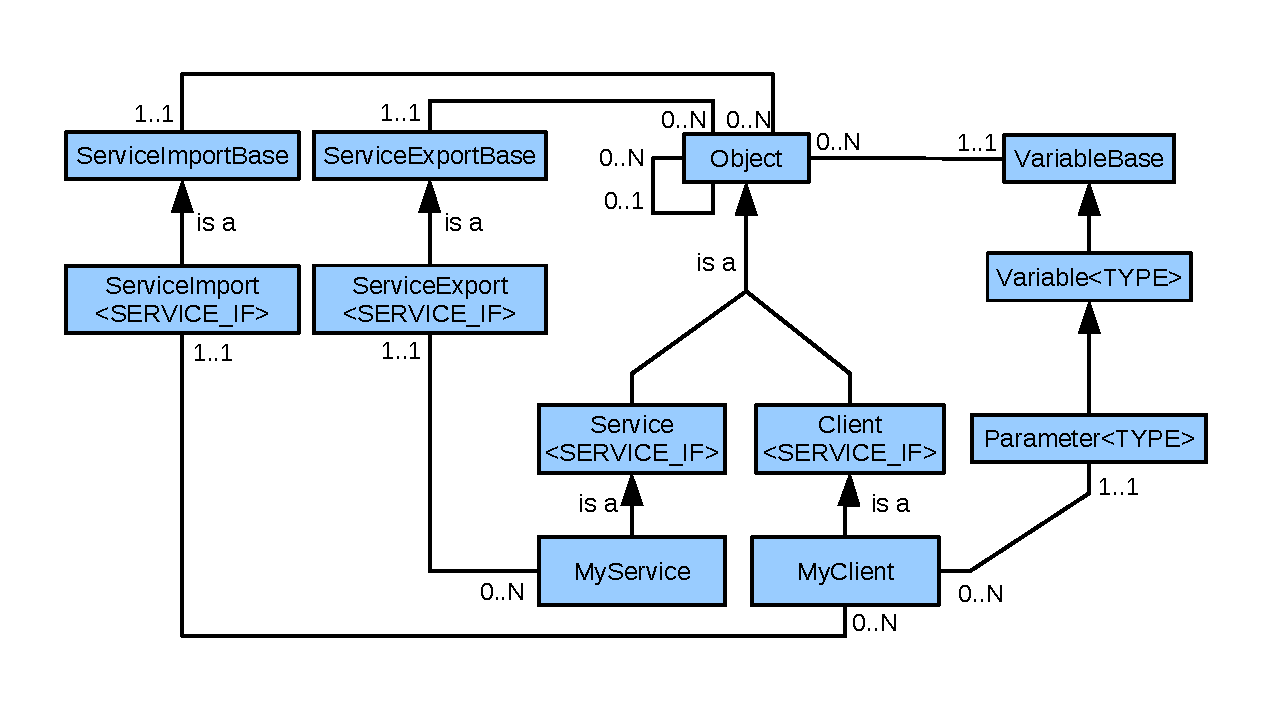
\includegraphics[width=\textwidth]{tms320c3x/fig_object_hierarchy.pdf}
	\end{center}
	\caption{Service/Client/Run-time Parameters Object hierarchy.}
	\label{fig:tms320c3x_object_hierarchy}
\end{figure}

\subsubsection{Building a service graph}
\label{tms320c3x_building_a_service_graph}

Using services implies building a service graph.
For instance, consider that the client is a loader, and the service is a memory.
The programmer creates objects \texttt{loader} and \texttt{memory}, see Figure~\ref{fig:tms320c3x_service_instanciation}.

\begin{figure}[h]
  \begin{center}
    \input{tms320c3x/service_instanciation}
    \caption{\label{fig:tms320c3x_service_instanciation} Client/Service instantiation.}
  \end{center}
\end{figure}

Object \texttt{loader} is a client because it needs a service (reading/writing in memory) from object \texttt{memory} to load the program.
\texttt{loader} has a member \texttt{import} named \texttt{memory\_import} whereas \texttt{memory} object has a member \texttt{export} named \texttt{memory\_export}.
The programmer connects the loader to the memory using \texttt{loader.memory\_import} and \texttt{memory.memory\_export}, see Figure~\ref{fig:tms320c3x_service_connection}.

\begin{figure}[h]
  \begin{center}
    \input{tms320c3x/service_connection}
    \caption{\label{fig:tms320c3x_service_connection} Import/Export connection.}
  \end{center}
\end{figure}

Once \hfill the \hfill programmer \hfill has \hfill created \hfill a \hfill service \hfill graph, \hfill he \hfill must \hfill perform \hfill a \hfill call \hfill to \hfill \texttt{ServiceManager::Setup()}.
\texttt{ServiceManager::Setup()} returns \texttt{true} if setup of each service and client in the graph has been successful, otherwise it returns \texttt{false}.

\subsubsection{Designing a service}

A service is a C++ object inheriting from template class \texttt{Service<SERVICE\_INTERFACE>} \ding{202}, see Figure~\ref{fig:tms320c3x_simple_service}.
\texttt{SERVICE\_INTERFACE} is a C++ abstract class defining the virtual methods implemented by the service.
To export its interface, a service must have a member of type \texttt{ServiceExport<SERVICE\_INTERFACE>} \ding{203}.
For normalization purposes, the service constructor should only take two parameters \ding{204}: the service name and the pointer to the parent (a container service).
The pointer to the parent is \texttt{null} if the service is a top level service (no parent).
The base \texttt{Object} constructor \ding{205} and the base \texttt{Service} constructor \ding{206} must be called with the name and the pointer to the parent.
\texttt{ServiceExport} member constructor must be called with the export name and a pointer to the owner, i.e. the service itself \ding{207}.

\begin{figure}[h]
  \begin{center}
    \input{tms320c3x/simple_service}
    \caption{\label{fig:tms320c3x_simple_service} Simple service.}
  \end{center}
\end{figure}

\subsubsection{Designing a client}

A client is a C++ object inheriting from template class \texttt{Client<SERVICE\_INTERFACE>} \ding{202}, see Figure~\ref{fig:tms320c3x_simple_client}.
\texttt{SERVICE\_INTERFACE} is a C++ abstract class defining the virtual methods implemented by the service the client can call.
To import an interface, a client must have a member of type \texttt{ServiceImport<SERVICE\_INTERFACE>} \ding{203}.
For normalization purposes, the client constructor should only take two parameters \ding{204}: the client name and the pointer to the parent (a container client).
The pointer to the parent is \texttt{null} if the client is a top level client (no parent).
The base \texttt{Object} constructor \ding{205} and the base \texttt{Client} constructor \ding{206} must be called with the name and the pointer to the parent.
\texttt{ServiceImport} member constructor must be called with the import name and a pointer to the owner, i.e. the client itself \ding{207}.


\begin{figure}[h]
  \begin{center}
    \input{tms320c3x/simple_client}
    \caption{\label{fig:tms320c3x_simple_client} Simple client.}
  \end{center}
\end{figure}

\subsubsection{Run-time parameters}

Run-time parameterization can be added to a service or a client.
``Run-time parameterization'' means that the service and/or client can be reconfigured at run-time.
It is opposed to ``Static parameterization'' or ``template parameterization'' which allows configuring a service and/or client at compilation-time.
To expose a member variable as a run-time parameter, a client/service must have a member variable of type \texttt{Parameter<TYPE>}, where \texttt{TYPE} is the C++ type of the exposed member variable, see Figure~\ref{fig:tms320c3x_run_time_parameter}.
Multiple \texttt{Parameter} variables with different \texttt{TYPE}s can be defined within a client/service.
Consider that a service would expose a member variable \texttt{x} \ding{202}.
An instance of class \texttt{Parameter} is defined as a member of the service \ding{203}. 
The parameter is bound to the exposed variable \ding{204} in the service/client constructor.

\begin{figure}[h]
  \begin{center}
    \input{tms320c3x/run_time_parameter}
    \caption{\label{fig:tms320c3x_run_time_parameter} Exposing a service/client member variable as a run-time parameter.}
  \end{center}
\end{figure}

\subsubsection{Setup Order}

As explained in section~\ref{tms320c3x_building_a_service_graph}, method \texttt{Setup} of class \texttt{ServiceManager} calls all \texttt{Setup} methods in the simulator. 
A problem may occur if setup order is important.
For instance, consider two services: service \texttt{A} and \texttt{B}. 
\texttt{A::Setup()} uses service \texttt{B}.
A correct setup order consist to first setup service \texttt{B} and then service \texttt{A}.
To solve such setup dependency, programmer should call method \texttt{ServiceExportBase::SetupDependsOn} (e.g. in the class constructor) so that the service manager can ensure correct setup order.
If the service manager finds a cyclic dependency, \texttt{ServiceManager::Setup()} fails: it generally means that clients and services have been badly designed.

\newpage
\subsection{Service Interfaces}
\label{tms320c3x_interfaces}

All service interfaces are declared in namespace \texttt{unisim::service::interfaces} and located in directory \texttt{unisim/service/interfaces}.

\subsubsection{Memory Interfaces}

These interfaces allow reading/writing from/to memory space. The memory interfaces comes in two flavors:
\begin{itemize}
\item Non-intrusive memory access (\texttt{unisim::service::interfaces::Memory}): It should not affect timing and data placement (e.g. in caches and TLBs).
\item Intrusive memory access (\texttt{unisim::service::interfaces::MemoryInjection}): It can affect timing and data placement.
\end{itemize}

\noindent The two C++ interfaces are:

\begin{center}
	\input{tms320c3x/memory_interface}
\end{center}

\begin{center}
	\input{tms320c3x/memory_injection_interface}
\end{center}

\noindent The arguments to methods \texttt{ReadMemory}, \texttt{InjectReadMemory}, \texttt{WriteMemory}, \texttt{InjectWriteMemory} are:
\begin{itemize}
\item \texttt{addr}: the starting address of the data transfer between the memory and the buffer
\item \texttt{buffer}: a pointer to the buffer of bytes
\item \texttt{size}: the length in bytes to transfer between the memory and the buffer
\end{itemize}

\subsubsection{Debugging Interfaces}

These interfaces are intended for the connection of the simulation components (e.g. CPU, memory, devices, \ldots) with a debugger (e.g. inline-debugger, GDB server, \ldots).

\textbf{Instruction disassembly}. CPU components provide a disassembly capability of the instruction set using the \texttt{unisim::service::interfaces::Disassembly} interface for the debbuger.

\begin{center}
	\input{tms320c3x/disassembly_interface}
\end{center}

\noindent Method \texttt{Disasm} arguments are:
\begin{itemize}
\item \texttt{addr}: the byte address of the instruction to disassemble
\item \texttt{next\_addr}: the byte address of the next instruction
\end{itemize}
\noindent and returns a string with the disassembly of the instruction.

\textbf{Register access}. A CPU or a device provides an access to its registers using the \texttt{unisim::service::interfaces::Registers} interface for the debugger.

\begin{center}
	\input{tms320c3x/registers_interface}
\end{center}

\noindent Method \texttt{GetRegister} arguments are:
\begin{itemize}
\item \texttt{name}: the name of the register to retrieve the register interface
\end{itemize}
\noindent and returns a pointer to an \texttt{unisim::util::debug::Register} interface.

\begin{center}
	\input{tms320c3x/register_interface}
\end{center}

\noindent Method \texttt{GetName} returns the register name.
\noindent Method \texttt{GetValue} fills in a buffer with the register value.
\noindent Method \texttt{SetValue} sets the register value from a buffer.
\noindent Method \texttt{GetSize} returns the register size in bytes.

\textbf{Step by step execution}. A simulation component (e.g. a CPU) leaves control to a debugger with the \texttt{unisim::service::interfaces::DebugYielding} interface.

\begin{center}
	\input{tms320c3x/debug_control_interface}
\end{center}

Method \texttt{FetchDebugCommand} takes the current program counter as argument and returns a command for the simulation component: either finish the simulation or execute one instruction.

\textbf{Monitoring memory accesses}. An instrumented simulation component provides a memory access trace using the \texttt{unisim::service::interfaces::MemoryAccessReporting} interface.
Such memory trace is useful for a debugger to monitor memory access.

\begin{center}
	\input{tms320c3x/memory_access_reporting_interface}
\end{center}

Method \texttt{ReportMemoryAccess} takes as arguments the memory access type (either read or write), the memory type (either data or instruction memory), the address of the access, and the size of the memory access.
Method \texttt{ReportFetchInstruction} takes as argument the address of instruction to be fetched.
Method \texttt{ReportCommitInstruction} takes as argument the address of instruction to be finalized along with its size.

\textbf{Trap reporting}. An instrumented simulation component informs a debugger about an important event using the \texttt{unisim::service::interfaces::TrapReporting} interface.
Such event is useful for a debugger to pause simulation when such event occurs.

\begin{center}
	\input{tms320c3x/trap_reporting_interface}
\end{center}

Method \texttt{ReportTrap} takes no arguments.

\textbf{Symbol}. A service (e.g. a loader) provides lookup to the symbol table using the \texttt{unisim::service::interfaces::SymbolTableLookup} interface.
This interface is useful for translating addresses to symbol names, and vice-versa.

\begin{center}
	\input{tms320c3x/symbol_table_lookup_interface}
\end{center}

\textbf{Efficient instrumentation.} To limit the impact on simulation performance of memory access instrumentation in the simulation components, such instrumentation can be enabled or disabled at run-time using interface \texttt{unisim::service::interfaces::MemoryAccessReportingControl}.

\begin{center}
	\input{tms320c3x/memory_access_reporting_control_interface}
\end{center}

\subsubsection{Loader Interface}

This interface provides basic informations about the loaded program.

\begin{center}
	\input{tms320c3x/loader_interface}
\end{center}

\subsubsection{Time Interface}

This interface provides the current simulation time of the component using it.


\begin{center}
	\input{tms320c3x/time_interface}
\end{center}

\subsubsection{TI C I/O Interface}

An instrumented TMS320C3X instruction set simulator provides a trace of \texttt{SWI} instructions using the \texttt{unisim::service::interfaces::ti\_c\_io} interface.
This interface is useful for the TI C I/O service to capture target program I/Os and translate them to host I/Os.

\begin{center}
	\input{tms320c3x/ti_c_io_interface}
\end{center}

\newpage
\subsection{Services}
\subsubsection{COFF loader service}
\label{tms320c3x_coff_loader}

This service provides UNISIM TMS320C3X simulator with a support for TI COFF v0, v1, and v2 binary files  either with little-endian or big-endian headers (see TMS320C3x/C4x Assembly Language Tools User’s Guide, Appendix A). 
The COFF loader service loads the programs into memory while setup (simulator initialization).
The loader can interpret \texttt{.cinit} section if option \texttt{-cr} of TI C cross-compiler has been used while building the target program (see \textit{TMS320C3x/C4x Optimizing C Compiler User’s Guide}, section 4.8.1: \textit{Autoinitialization of variables and constants}).
To configure the COFF loader service see Section~\ref{tms320c3x_configuration}.
The source code of COFF loader service is located in directory \texttt{unisim/service/loader/coff\_loader}.
\noindent The table below summarizes the COFF Loader service API:

\begin{center}
	\tablehead{\hline}
	\tabletail{\hline}
	\begin{supertabular}{|p{7.5cm}|p{7.5cm}|}
		\hline
		\multicolumn{2}{|l|}{\textbf{\Large Service COFF Loader}}\\
		\hline
		\multicolumn{1}{|p{7.5cm}}{\textbf{Class Name:} \newline \texttt{unisim::service::loader::coff\_loader}\newline$\hookrightarrow$\texttt{::CoffLoader}} & \multicolumn{1}{p{7.5cm}|}{\textbf{Header:} \newline \texttt{unisim/service/loader/coff\_loader}\newline$\hookrightarrow$\texttt{/coff\_loader.hh}}\\
		\multicolumn{2}{|l|}{}\\
		\multicolumn{2}{|p{15cm}|}{\textbf{Description:} \newline The COFF loader service allows to load a COFF binary program into a memory and fill a symbol table. The loader also provides information about the loaded file such as the code and data locations (base address and size). The COFF loader loads the program during setup.}\\
		\hline
		\hline
		\multicolumn{2}{|c|}{\textbf{\large Template Parameters}}\\
		\hline
		\multicolumn{1}{|p{7.5cm}}{\textbf{Name:} \texttt{MEMORY\_ADDR}} & \multicolumn{1}{p{7.5cm}|}{\textbf{Type:} \texttt{class}}\\
		\multicolumn{2}{|p{15cm}|}{\textbf{Default value:} \texttt{none}}\\
		\multicolumn{2}{|l|}{}\\
		\multicolumn{2}{|p{15cm}|}{\textbf{Description:} \newline This is the C++ type of a memory address (e.g. \texttt{uint32\_t} or \texttt{uint64\_t}).}\\
		\hline
		\hline
		\multicolumn{2}{|c|}{\textbf{\large Run-Time Parameters}}\\
		\hline
		\multicolumn{1}{|p{7.5cm}}{\textbf{Name:} \texttt{filename}} & \multicolumn{1}{p{7.5cm}|}{\textbf{Type:} \texttt{string}}\\
		\multicolumn{2}{|p{15cm}|}{\textbf{Default value:} empty string}\\
		\multicolumn{2}{|l|}{}\\
		\multicolumn{2}{|p{15cm}|}{\textbf{Description:} \newline The COFF file name to load into the connected memory.}\\
		\hline
		\hline
		\multicolumn{1}{|p{7.5cm}}{\textbf{Name:} \texttt{dump-headers}} & \multicolumn{1}{p{7.5cm}|}{\textbf{Type:} \texttt{boolean}}\\
		\multicolumn{2}{|p{15cm}|}{\textbf{Default value:} false}\\
		\multicolumn{2}{|l|}{}\\
		\multicolumn{2}{|p{15cm}|}{\textbf{Description:} \newline If true this parameter makes the COFF loader print the file headers on the screen (file header, section headers, symbol table \ldots) while loading the program.}\\
		\hline
		\multicolumn{2}{|c|}{\textbf{\large Service Exports}}\\
		\hline
		\multicolumn{1}{|p{7.5cm}}{\textbf{Name:} \texttt{logger\_export}} & \multicolumn{1}{p{7.5cm}|}{\textbf{Interface:} \newline \texttt{unisim::service::interfaces::} \newline$\hookrightarrow$\texttt{Loader<MEMORY\_ADDR>}}\\
		\multicolumn{2}{|l|}{}\\
		\multicolumn{2}{|p{15cm}|}{\textbf{Description:} \newline The COFF loader provides information about the code and data location through this export.}\\
		\hline
		\multicolumn{1}{|p{7.5cm}}{\textbf{Name:} \texttt{symbol\_table\_lookup\_export}} & \multicolumn{1}{p{7.5cm}|}{\textbf{Interface:} \newline \texttt{unisim::service::interfaces::} \newline$\hookrightarrow$\texttt{SymbolTableLookup<MEMORY\_ADDR>}}\\
		\multicolumn{2}{|l|}{}\\
		\multicolumn{2}{|p{15cm}|}{\textbf{Description:} \newline The COFF loader provides symbol lookup through this export.}\\
		\hline
		\hline
		\multicolumn{2}{|c|}{\textbf{\large Service Imports}}\\
		\hline
		\multicolumn{1}{|p{7.5cm}}{\textbf{Name:} \texttt{memory\_import} \newline \textbf{Mandatory connected:} no} & \multicolumn{1}{p{7.5cm}|}{\textbf{Interface:} \newline \texttt{unisim::service::interfaces::} \newline$\hookrightarrow$\texttt{Memory<uint32\_t>}}\\
		\multicolumn{2}{|l|}{}\\
		\multicolumn{2}{|p{15cm}|}{\textbf{Description:} \newline The COFF loader accesses to the memory through this import.}\\
		\hline
	\end{supertabular}
\end{center}

\newpage
\subsubsection{TI C I/O service}
\label{tms320c3x_ti_c_io}

This service provides low level I/O (open, read, write, close, \ldots) support on the host machine for target programs.
The TI Run-time support libraries (\texttt{RTS*.lib}) implement a software stack for standard C I/Os (see \textit{TMS320C3x/C4x Optimizing C Compiler User’s Guide} (SPRU034H, June 1998), Appendix B).
A development board debugger captures target program I/Os at \texttt{C\$\$IO\$\$}.
The Run-time support library puts the I/Os in a communication buffer (\texttt{\_\_CIOBUF\_}) that the development board debugger translates to host I/Os.
The debugger also captures target program termination at \texttt{C\$\$EXIT}.
The UNISIM TI C I/O service captures and translates target program I/Os and termination in the same manner as a development board built-in debugger.
To configure the TI C I/O service see Section~\ref{tms320c3x_configuration}.
The source code of the COFF loader service is located in directory \texttt{unisim/service/os/ti\_c\_io}.
\noindent The table below summarizes the TI C I/O service API:

\begin{center}
	\tablehead{\hline}
	\tabletail{\hline}
	\begin{supertabular}{|p{7.5cm}|p{7.5cm}|}
		\hline
		\multicolumn{2}{|l|}{\textbf{\Large Service TI C I/O}}\\
		\hline
		\multicolumn{1}{|p{7.5cm}}{\textbf{Class Name:} \newline \texttt{unisim::service::os::ti\_c\_io}\newline$\hookrightarrow$\texttt{::TI\_C\_IO}} & \multicolumn{1}{p{7.5cm}|}{\textbf{Header:} \newline \texttt{unisim/service/os/ti\_c\_io}\newline$\hookrightarrow$\texttt{/ti\_c\_io.hh}}\\
		\multicolumn{2}{|l|}{}\\
		\multicolumn{2}{|p{15cm}|}{\textbf{Description:} \newline The TI C I/O service provides low level I/O (open, read, write, close, \ldots) support on the host machine for target programs.}\\
		\hline
		\hline
		\multicolumn{2}{|c|}{\textbf{\large Template Parameters}}\\
		\hline
		\multicolumn{1}{|p{7.5cm}}{\textbf{Name:} \texttt{MEMORY\_ADDR}} & \multicolumn{1}{p{7.5cm}|}{\textbf{Type:} \texttt{class}}\\
		\multicolumn{2}{|p{15cm}|}{\textbf{Default value:} \texttt{none}}\\
		\multicolumn{2}{|l|}{}\\
		\multicolumn{2}{|p{15cm}|}{\textbf{Description:} \newline This is the C++ type of a memory address (e.g. uint32\_t or uint64\_t).}\\
		\hline
		\hline
		\multicolumn{2}{|c|}{\textbf{\large Run-Time Parameters}}\\
		\hline
		\multicolumn{1}{|p{7.5cm}}{\textbf{Name:} \texttt{ti\_c\_io.enable}} & \multicolumn{1}{p{7.5cm}|}{\textbf{Type:} \texttt{bool}}\\
		\multicolumn{2}{|p{15cm}|}{\textbf{Default value:} \texttt{false}}\\
		\multicolumn{2}{|l|}{}\\
		\multicolumn{2}{|p{15cm}|}{\textbf{Description:} \newline Enable/disable TI C I/O support.}\\
		\hline
		\multicolumn{1}{|p{7.5cm}}{\textbf{Name:} \texttt{ti-c-io.warning-as-error}} & \multicolumn{1}{p{7.5cm}|}{\textbf{Type:} \texttt{bool}}\\
		\multicolumn{2}{|p{15cm}|}{\textbf{Default value:} \texttt{false}}\\
		\multicolumn{2}{|l|}{}\\
		\multicolumn{2}{|p{15cm}|}{\textbf{Description:} \newline Whether Warnings are considered as error or not.}\\
		\hline
		\multicolumn{1}{|p{7.5cm}}{\textbf{Name:} \texttt{ti-c-io.pc-register-name}} & \multicolumn{1}{p{7.5cm}|}{\textbf{Type:} \texttt{string}}\\
		\multicolumn{2}{|p{15cm}|}{\textbf{Default value:} \texttt{"PC"}}\\
		\multicolumn{2}{|l|}{}\\
		\multicolumn{2}{|p{15cm}|}{\textbf{Description:} \newline Name of the CPU program counter register.}\\
		\hline
		\multicolumn{1}{|p{7.5cm}}{\textbf{Name:} \texttt{ti-c-io.c-io-buffer-symbol-name}} & \multicolumn{1}{p{7.5cm}|}{\textbf{Type:} \texttt{string}}\\
		\multicolumn{2}{|p{15cm}|}{\textbf{Default value:} \texttt{"\_\_CIOBUF\_"}}\\
		\multicolumn{2}{|l|}{}\\
		\multicolumn{2}{|p{15cm}|}{\textbf{Description:} \newline C I/O buffer symbol name.}\\
		\hline
		\multicolumn{1}{|p{7.5cm}}{\textbf{Name:} \texttt{ti-c-io.c-io-breakpoint-}\newline$\hookrightarrow$\texttt{symbol-name}} & \multicolumn{1}{p{7.5cm}|}{\textbf{Type:} \texttt{string}}\\
		\multicolumn{2}{|p{15cm}|}{\textbf{Default value:} \texttt{"C\$\$IO\$\$"}}\\
		\multicolumn{2}{|l|}{}\\
		\multicolumn{2}{|p{15cm}|}{\textbf{Description:} \newline C I/O breakpoint symbol name. The TI C I/O service installs a \texttt{SWI} instruction at this point to capture target program I/O.}\\
		\hline
		\multicolumn{1}{|p{7.5cm}}{\textbf{Name:} \texttt{ti-c-io.c-exit-breakpoint-}\newline$\hookrightarrow$\texttt{symbol-name}} & \multicolumn{1}{p{7.5cm}|}{\textbf{Type:} \texttt{string}}\\
		\multicolumn{2}{|p{15cm}|}{\textbf{Default value:} \texttt{"C\$\$EXIT"}}\\
		\multicolumn{2}{|l|}{}\\
		\multicolumn{2}{|p{15cm}|}{\textbf{Description:} \newline C EXIT breakpoint symbol name. The TI C I/O service installs a \texttt{SWI} instruction at this point to capture target program exit.}\\
		\hline
		\multicolumn{1}{|p{7.5cm}}{\textbf{Name:} \texttt{ti-c-io.verbose-all}} & \multicolumn{1}{p{7.5cm}|}{\textbf{Type:} \texttt{bool}}\\
		\multicolumn{2}{|p{15cm}|}{\textbf{Default value:} \texttt{false}}\\
		\multicolumn{2}{|l|}{}\\
		\multicolumn{2}{|p{15cm}|}{\textbf{Description:} \newline Globally enable/disable verbosity of TI C I/O service.}\\
		\hline
		\multicolumn{1}{|p{7.5cm}}{\textbf{Name:} \texttt{ti-c-io.verbose-io}} & \multicolumn{1}{p{7.5cm}|}{\textbf{Type:} \texttt{bool}}\\
		\multicolumn{2}{|p{15cm}|}{\textbf{Default value:} \texttt{false}}\\
		\multicolumn{2}{|l|}{}\\
		\multicolumn{2}{|p{15cm}|}{\textbf{Description:} \newline Enable/disable verbosity of TI C I/O service while performing I/Os.}\\
		\hline
		\multicolumn{1}{|p{7.5cm}}{\textbf{Name:} \texttt{ti-c-io.verbose-setup}} & \multicolumn{1}{p{7.5cm}|}{\textbf{Type:} \texttt{bool}}\\
		\multicolumn{2}{|p{15cm}|}{\textbf{Default value:} \texttt{false}}\\
		\multicolumn{2}{|l|}{}\\
		\multicolumn{2}{|p{15cm}|}{\textbf{Description:} \newline Enable/disable verbosity of TI C I/O service while setup.}\\
		\hline
		\hline
		\multicolumn{2}{|c|}{\textbf{\large Service Exports}}\\
		\hline
		\multicolumn{1}{|p{7.5cm}}{\textbf{Name:} \texttt{ti\_c\_io\_export}} & \multicolumn{1}{p{7.5cm}|}{\textbf{Interface:} \newline \texttt{unisim::interfaces::} \newline$\hookrightarrow$\texttt{TI\_C\_IO<MEMORY\_ADDR>}}\\
		\multicolumn{2}{|l|}{}\\
		\multicolumn{2}{|p{15cm}|}{\textbf{Description:} \newline The TI C I/O provides target to host I/O translation through this service export.}\\
		\hline
		\hline
		\multicolumn{2}{|c|}{\textbf{\large Service Imports}}\\
		\hline
		\multicolumn{1}{|p{7.5cm}}{\textbf{Name:} \texttt{memory\_import}} & \multicolumn{1}{p{7.5cm}|}{\textbf{Interface:} \newline \texttt{unisim::service::interfaces::} \newline$\hookrightarrow$\texttt{Memory<MEMORY\_ADDR>}}\\
		\multicolumn{2}{|p{15cm}|}{\textbf{Mandatory connected:} no}\\
		\multicolumn{2}{|l|}{}\\
		\multicolumn{2}{|p{15cm}|}{\textbf{Description:} \newline The TI C I/O service accesses to the memory while setup through this import. While in setup it installs two \texttt{SWI} instructions to capture both target I/O and program exit.}\\
		\hline
		\multicolumn{1}{|p{7.5cm}}{\textbf{Name:} \texttt{memory\_injection\_import}} & \multicolumn{1}{p{7.5cm}|}{\textbf{Interface:} \newline \texttt{unisim::service::interfaces::} \newline$\hookrightarrow$\texttt{MemoryInjection<MEMORY\_ADDR>}}\\
		\multicolumn{2}{|p{15cm}|}{\textbf{Mandatory connected:} no}\\
		\multicolumn{2}{|l|}{}\\
		\multicolumn{2}{|p{15cm}|}{\textbf{Description:} \newline The TI C I/O service accesses to the memory while simulation through this import. It accesses to the I/O buffer in the target program memory and then interprete the content of this buffer to translate target program I/Os to host I/Os.}\\
		\hline
		\multicolumn{1}{|p{7.5cm}}{\textbf{Name:} \texttt{registers\_import} \newline \textbf{Mandatory connected:} yes} & \multicolumn{1}{p{7.5cm}|}{\textbf{Interface:} \newline \texttt{unisim::service::interfaces} \newline$\hookrightarrow$\texttt{::Registers}}\\
		\multicolumn{2}{|l|}{}\\
		\multicolumn{2}{|p{15cm}|}{\textbf{Description:} \newline This service import should be connected to a CPU module. The TI C I/O service calls method \texttt{GetRegister} through this service import to get an interface to the CPU registers. The TI C I/O service uses methods \texttt{GetName}, \texttt{GetValue}, \texttt{GetSize} and \texttt{SetValue} of that interface to access to CPU registers. This import is mainly used to get the current PC, so that the TI C I/O service can distinguish target program I/Os from target program exit.}\\
		\hline
		\multicolumn{1}{|p{7.5cm}}{\textbf{Name:} \texttt{symbol\_table\_lookup\_import} \newline \textbf{Mandatory connected:} yes} & \multicolumn{1}{p{7.5cm}|}{\textbf{Interface:} \newline \texttt{unisim::service::interfaces} \newline$\hookrightarrow$\texttt{::SymbolTableLookup<MEMORY\_ADDR>}}\\
		\multicolumn{2}{|l|}{}\\
		\multicolumn{2}{|p{15cm}|}{\textbf{Description:} \newline The TI C I/O service uses this service import to get the address of the breakpoints and I/O buffer from their symbol name.}\\
		\hline
	\end{supertabular}
\end{center}

\newpage
\subsubsection{Inline debugger}
\label{tms320c3x_inline_debugger}

The inline debugger service is a built-in debugger with a text-based user interface, see~\ref{tms320c3x_inline_debug}. 
It provides instruction level debugging of the target program.
\noindent Table below summarizes the inline debugger service API:

\begin{center}
	\tablehead{\hline}
	\tabletail{\hline}
	\begin{supertabular}{|p{7.5cm}|p{7.5cm}|}
		\hline
		\multicolumn{2}{|l|}{\textbf{\Large Service Inline Debugger}}\\
		\hline
		\multicolumn{1}{|p{7.5cm}}{\textbf{Class Name:} \newline \texttt{unisim::service::debug}\newline$\hookrightarrow$\texttt{::inline\_debugger::InlineDebugger}} & \multicolumn{1}{p{7.5cm}|}{\textbf{Header:} \newline \texttt{unisim/service/debug}\newline$\hookrightarrow$\texttt{/inline\_debugger/inline\_debugger.hh}}\\
		\multicolumn{2}{|l|}{}\\
		\multicolumn{2}{|p{15cm}|}{\textbf{Description:} \newline The inline debugger service provides a simple text-based interface to interactively debug a target application running on a CPU module for the user. The debug is at the instruction level. The inline debugger may be connected to a CPU module.}\\
		\hline
		\hline
		\multicolumn{2}{|c|}{\textbf{\large Template Parameters}}\\
		\hline
		\multicolumn{1}{|p{7.5cm}}{\textbf{Name:} \texttt{ADDRESS}} & \multicolumn{1}{p{7.5cm}|}{\textbf{Type:} \texttt{class}}\\
		\multicolumn{2}{|p{15cm}|}{\textbf{Default value:} none}\\
		\multicolumn{2}{|l|}{}\\
		\multicolumn{2}{|p{15cm}|}{\textbf{Description:} \newline This is the C++ type of a memory address (e.g. uint32\_t or uint64\_t).}\\
		\hline
		\hline
		\multicolumn{2}{|c|}{\textbf{\large Run-time parameters}}\\
		\hline
		\multicolumn{1}{|p{7.5cm}}{\textbf{Name:} \texttt{inline-debugger.memory-atom-size}} & \multicolumn{1}{p{7.5cm}|}{\textbf{Type:} \texttt{unsigned integer}}\\
		\multicolumn{2}{|p{15cm}|}{\textbf{Default value:} \texttt{1}}\\
		\multicolumn{2}{|l|}{}\\
		\multicolumn{2}{|p{15cm}|}{\textbf{Description:} \newline Size of the smallest addressable element in memory.}\\
		\hline
		\hline
		\multicolumn{2}{|c|}{\textbf{\large Service Exports}}\\
		\hline
		\multicolumn{1}{|p{7.5cm}}{\textbf{Name:} \texttt{debug\_control\_export}} & \multicolumn{1}{p{7.5cm}|}{\textbf{Interface:} \newline \texttt{unisim::service::interfaces} \newline$\hookrightarrow$\texttt{::DebugControl<ADDRESS>}}\\
		\multicolumn{2}{|l|}{}\\
		\multicolumn{2}{|p{15cm}|}{\textbf{Description:} \newline This service export should be connected to a CPU module. The CPU module calls method \texttt{FetchDebugCommand} through its service import to leave control to the debugger and fetch a new debug command.}\\
		\hline
		\multicolumn{1}{|p{7.5cm}}{\textbf{Name:} \texttt{memory\_access\_reporting\_export}} & \multicolumn{1}{p{7.5cm}|}{\textbf{Interface:} \newline \texttt{unisim::service::interfaces} \newline$\hookrightarrow$\texttt{MemoryAccessReporting<ADDRESS>}}\\
		\multicolumn{2}{|l|}{}\\
		\multicolumn{2}{|p{15cm}|}{\textbf{Description:} \newline This service export should be connected to a CPU module. The CPU module calls methods \texttt{ReportMemoryAccess}, \texttt{ReportFetchInstruction} and \texttt{ReportCommitInstruction} through its service import. This allows the debugger to spy memory accesses and thus handle breakpoints and watchpoints.}\\
		\hline
		\multicolumn{1}{|p{7.5cm}}{\textbf{Name:} \texttt{trap\_reporting\_export}} & \multicolumn{1}{p{7.5cm}|}{\textbf{Interface:} \newline \texttt{unisim::service::interfaces} \newline$\hookrightarrow$\texttt{::TrapReporting}}\\
		\multicolumn{2}{|l|}{}\\
		\multicolumn{2}{|p{15cm}|}{\textbf{Description:} \newline This service export should be connected to a CPU module. A CPU module calls method \texttt{ReportTrap} through its service import. This allows the debugger to break execution on the simulated CPU once a trap condition is detected by the CPU module.}\\
		\hline
		\hline
		\multicolumn{2}{|c|}{\textbf{\large Service Imports}}\\
		\hline
		\multicolumn{1}{|p{7.5cm}}{\textbf{Name:} \texttt{disasm\_import} \newline \textbf{Mandatory connected:} yes} & \multicolumn{1}{p{7.5cm}|}{\textbf{Interface:} \newline \texttt{unisim::service::interfaces} \newline$\hookrightarrow$\texttt{::Disassembly<ADDRESS>}}\\
		\multicolumn{2}{|l|}{}\\
		\multicolumn{2}{|p{15cm}|}{\textbf{Description:} \newline This service import should be connected to a CPU module. The CPU module should implement method \texttt{Disassemble} which provides disassembling of the instructions for the debugger.}\\
		\hline
		\multicolumn{1}{|p{7.5cm}}{\textbf{Name:} \texttt{memory\_import} \newline \textbf{Mandatory connected:} yes} & \multicolumn{1}{p{7.5cm}|}{\textbf{Interface:} \newline \texttt{unisim::service::interfaces} \newline$\hookrightarrow$\texttt{::Memory<ADDRESS>}}\\
		\multicolumn{2}{|l|}{}\\
		\multicolumn{2}{|p{15cm}|}{\textbf{Description:} \newline This service import should be connected to a CPU or a memory module. The debugger uses this service import to access to memory using methods \texttt{ReadMemory} and \texttt{WriteMemory}.}\\
		\hline
		\multicolumn{1}{|p{7.5cm}}{\textbf{Name:} \texttt{memory\_access\_reporting\newline$\hookrightarrow$\_control\_import} \newline \textbf{Mandatory connected:} no} & \multicolumn{1}{p{7.5cm}|}{\textbf{Interface:} \newline \texttt{unisim::service::interfaces} \newline$\hookrightarrow$\texttt{::MemoryAccessReportingControl}}\\
		\multicolumn{2}{|l|}{}\\
		\multicolumn{2}{|p{15cm}|}{\textbf{Description:} \newline This service import should be connected to a CPU module. The debugger calls methods \texttt{RequiresMemoryAccessReporting} and \texttt{RequiresFinishedInstructionReporting} through this service import to enable/disable memory access reporting from the CPU module.}\\
		\hline
		\multicolumn{1}{|p{7.5cm}}{\textbf{Name:} \texttt{registers\_import} \newline \textbf{Mandatory connected:} yes} & \multicolumn{1}{p{7.5cm}|}{\textbf{Interface:} \newline \texttt{unisim::service::interfaces} \newline$\hookrightarrow$\texttt{::Registers}}\\
		\multicolumn{2}{|l|}{}\\
		\multicolumn{2}{|p{15cm}|}{\textbf{Description:} \newline This service import should be connected to a CPU module. The debugger calls method \texttt{GetRegister} through this service import to get an interface to the CPU registers. The debugger uses methods \texttt{GetName}, \texttt{GetValue}, \texttt{GetSize} and \texttt{SetValue} of that interface to access to CPU registers.}\\
		\hline
		\multicolumn{1}{|p{7.5cm}}{\textbf{Name:} \texttt{symbol\_table\_lookup\_import} \newline \textbf{Mandatory connected:} no} & \multicolumn{1}{p{7.5cm}|}{\textbf{Interface:} \newline \texttt{unisim::service::interfaces} \newline$\hookrightarrow$\texttt{::SymbolTableLookup}}\\
		\multicolumn{2}{|l|}{}\\
		\multicolumn{2}{|p{15cm}|}{\textbf{Description:} \newline This service import should be connected to a symbol table. The debugger calls method \texttt{FindSymbol}, \texttt{FindSymbolByAddr}, \texttt{FindSymbolByName} through this service import to translate addresses to symbols and vice-versa.}\\
		\hline
	\end{supertabular}
\end{center}

\subsubsection{GDB server}
\label{tms320c3x_gdb_server}

The GDB server service emulates the GDB remote serial protocol over TCP/IP (see \textit{Debugging with GDB}, Appendix D. \textit{GDB Remote serial protocol}), so that a GDB client can connect to the simulator and debug the target program as if it were run on the real hardware.
This service uses an architecture XML description file defined by the \texttt{architecture-description-filename} run-time parameter (see table below).
A sample configuration file for a dummy \texttt{XYZ} big-endian architecture, with four 32-bit general purpose registers named \texttt{r0}, \texttt{r1}, \texttt{r2}, \texttt{r3} and a program counter named \texttt{pc} would be the following:
\begin{verbatim}
<architecture name="XYZ" endian="big">
    <program_counter name="pc"/>
    <register name="r0" size="4"/>
    <register name="r1" size="4"/>
    <register name="r2" size="4"/>
    <register name="r3" size="4"/>
</architecture>
\end{verbatim}

\noindent Table below summarizes the GDB server service API:

\begin{center}
	\tablehead{\hline}
	\tabletail{\hline}
	\begin{supertabular}{|p{7.5cm}|p{7.5cm}|}
		\hline
		\multicolumn{2}{|l|}{\textbf{\Large Service GDB Server}}\\
		\hline
		\multicolumn{1}{|p{7.5cm}}{\textbf{Class Name:} \newline \texttt{unisim::service::debug}\newline$\hookrightarrow$\texttt{::gdb\_server::GDBServer}} & \multicolumn{1}{p{7.5cm}|}{\textbf{Header:} \newline \texttt{unisim/service/debug}\newline$\hookrightarrow$\texttt{/gdb\_server/gdb\_server.hh}}\\
		\multicolumn{2}{|l|}{}\\
		\multicolumn{2}{|p{15cm}|}{\textbf{Description:} \newline The GDB server service allows debugging a software running on a simulated hardware by connecting (over TCP/IP) a GDB client to it (and thus to the simulator). The GDB client can be either the standard text based client (i.e. command \texttt{gdb}), a graphical front-end to GDB (e.g. \texttt{ddd}), or even Eclipse CDT. The GDB server service directly speaks to the GDB serial remote protocol (over TCP/IP), so that a GDB client can connect (over TCP/IP) to the simulator using GDB command \texttt{target remote}. The GDB server service may be connected to a CPU module.}\\
		\hline
		\hline
		\multicolumn{2}{|c|}{\textbf{\large Template Parameters}}\\
		\hline
		\multicolumn{1}{|p{7.5cm}}{\textbf{Name:} \texttt{ADDRESS}} & \multicolumn{1}{p{7.5cm}|}{\textbf{Type:} \texttt{class}}\\
		\multicolumn{2}{|p{15cm}|}{\textbf{Default value:} none}\\
		\multicolumn{2}{|l|}{}\\
		\multicolumn{2}{|p{15cm}|}{\textbf{Description:} \newline This is the C++ type of a memory address (e.g. uint32\_t or uint64\_t).}\\
		\hline
		\hline
		\multicolumn{2}{|c|}{\textbf{\large Run-Time Parameters}}\\
		\hline
		\multicolumn{1}{|p{7.5cm}}{\textbf{Name:} \texttt{tcp-port}} & \multicolumn{1}{p{7.5cm}|}{\textbf{Type:} \texttt{int}}\\
		\multicolumn{2}{|p{15cm}|}{\textbf{Default value:} \texttt{12345}}\\
		\multicolumn{2}{|l|}{}\\
		\multicolumn{2}{|p{15cm}|}{\textbf{Description:} \newline The TCP port used by GDB server service to communicate with the GDB client.}\\
		\hline
		\multicolumn{1}{|p{7.5cm}}{\textbf{Name:} \texttt{architecture-description\newline$\hookrightarrow$-filename}} & \multicolumn{1}{p{7.5cm}|}{\textbf{Type:} \texttt{string}}\\
		\multicolumn{2}{|p{15cm}|}{\textbf{Default value:} empty string}\\
		\multicolumn{2}{|l|}{}\\
		\multicolumn{2}{|p{15cm}|}{\textbf{Description:} \newline The path to the architecture description file that the GDB server service must use. The description file provides retargetability to the GDB server service. The following files brings support of the ARM, PowerPC, TMS320C3X and HCS12X processors to the GDB server service: 
		\begin{itemize}
			\item \texttt{unisim/service/debug/gdb\_server/gdb\_armv4l.xml}
			\item \texttt{unisim/service/debug/gdb\_server/gdb\_armv5b.xml}
			\item \texttt{unisim/service/debug/gdb\_server/gdb\_powerpc.xml}
			\item \texttt{unisim/service/debug/gdb\_server/gdb\_tms320c3x.xml}
			\item \texttt{unisim/service/debug/gdb\_server/gdb\_hcs12x.xml}
		\end{itemize}
		}\\
		\hline
		\hline
		\multicolumn{2}{|c|}{\textbf{\large Service Exports}}\\
		\hline
		\multicolumn{1}{|p{7.5cm}}{\textbf{Name:} \texttt{debug\_control\_export}} & \multicolumn{1}{p{7.5cm}|}{\textbf{Interface:} \newline \texttt{unisim::service::interfaces} \newline$\hookrightarrow$\texttt{::DebugControl<ADDRESS>}}\\
		\multicolumn{2}{|l|}{}\\
		\multicolumn{2}{|p{15cm}|}{\textbf{Description:} \newline This service export should be connected to a CPU module. The CPU module calls method \texttt{FetchDebugCommand} through its service import to leave control to the debugger and fetch a new debug command.}\\
		\hline
		\multicolumn{1}{|p{7.5cm}}{\textbf{Name:} \texttt{memory\_access\_reporting\_export}} & \multicolumn{1}{p{7.5cm}|}{\textbf{Interface:} \newline \texttt{unisim::service::interfaces} \newline$\hookrightarrow$\texttt{MemoryAccessReporting<ADDRESS>}}\\
		\multicolumn{2}{|l|}{}\\
		\multicolumn{2}{|p{15cm}|}{\textbf{Description:} \newline This service export should be connected to a CPU module. The CPU module calls methods \texttt{ReportMemoryAccess}, \texttt{ReportFetchInstruction} and \texttt{ReportCommitInstruction} through its service import. This allows the debugger to spy memory accesses and thus handle breakpoints and watchpoints.}\\
		\hline
		\multicolumn{1}{|p{7.5cm}}{\textbf{Name:} \texttt{trap\_reporting\_export}} & \multicolumn{1}{p{7.5cm}|}{\textbf{Interface:} \newline \texttt{unisim::service::interfaces} \newline$\hookrightarrow$\texttt{::TrapReporting}}\\
		\multicolumn{2}{|l|}{}\\
		\multicolumn{2}{|p{15cm}|}{\textbf{Description:} \newline This service export should be connected to a CPU module. A CPU module calls method \texttt{ReportTrap} through its service import. This allows the debugger to break execution on the simulated CPU when a trap condition is detected by the CPU module.}\\
		\hline
		\hline
		\multicolumn{2}{|c|}{\textbf{\large Service Imports}}\\
		\hline
		\multicolumn{1}{|p{7.5cm}}{\textbf{Name:} \texttt{memory\_import} \newline \textbf{Mandatory connected:} yes} & \multicolumn{1}{p{7.5cm}|}{\textbf{Interface:} \newline \texttt{unisim::service::interfaces} \newline$\hookrightarrow$\texttt{::Memory<ADDRESS>}}\\
		\multicolumn{2}{|l|}{}\\
		\multicolumn{2}{|p{15cm}|}{\textbf{Description:} \newline This service import should be connected to a CPU or a memory module. The debugger uses this service import to access to memory using methods \texttt{ReadMemory} and \texttt{WriteMemory}.}\\
		\hline
		\multicolumn{1}{|p{7.5cm}}{\textbf{Name:} \texttt{memory\_access\_reporting\newline$\hookrightarrow$\_control\_import} \newline \textbf{Mandatory connected:} no} & \multicolumn{1}{p{7.5cm}|}{\textbf{Interface:} \newline \texttt{unisim::service::interfaces} \newline$\hookrightarrow$\texttt{::MemoryAccessReportingControl}}\\
		\multicolumn{2}{|l|}{}\\
		\multicolumn{2}{|p{15cm}|}{\textbf{Description:} \newline This service import should be connected to a CPU module. The debugger calls methods \texttt{RequiresMemoryAccessReporting} and \texttt{RequiresFinishedInstructionReporting} through this service import to enable/disable memory access reporting from the CPU module.}\\
		\hline
		\multicolumn{1}{|p{7.5cm}}{\textbf{Name:} \texttt{registers\_import} \newline \textbf{Mandatory connected:} yes} & \multicolumn{1}{p{7.5cm}|}{\textbf{Interface:} \newline \texttt{unisim::service::interfaces} \newline$\hookrightarrow$\texttt{::Registers}}\\
		\multicolumn{2}{|l|}{}\\
		\multicolumn{2}{|p{15cm}|}{\textbf{Description:} \newline This service import should be connected to a CPU module. The debugger calls method \texttt{GetRegister} through this service import to get an interface to the CPU registers. The debugger uses methods \texttt{GetName}, \texttt{GetValue}, \texttt{GetSize} and \texttt{SetValue} of that interface to access to CPU registers.}\\
		\hline
	\end{supertabular}
\end{center}

\newpage
\subsubsection{Built-in Logger}
\label{tms320c3x_logger}

UNISIM provides you a centralized log system to debug modules and simulators. It should be used to show all debug messages, instead of using the traditional C++ stream output mechanism (\texttt{cerr} and \texttt{cout}). However, as you will see below the UNISIM log system works much like the C++ stream output mechanism.

It provides the following advantages:
\begin{itemize}
\item Categorization: messages can be categorized on information, warning and error messages
\item Atomic messages: messages will not be mixed (something which happens when programming concurrent/parallel systems like UNISIM/SystemC)
\item Multiple outputs: your messages can be written simultaneously to different outputs, for example:
	\begin{itemize}
	\item console (error output or standard output)
	\item raw file
	\item XML formatted file
	\item ...
	\end{itemize}
\item Simple configuration: the log system configuration is integrated to the UNISIM parameter mechanism provided by UNISIM service, see~\ref{tms320c3x_configuration}.
\end{itemize}

To use the UNISIM logger you need to include “unisim/kernel/logger/logger.hh” and declare that you are using the unisim::kernel::logger namespace:

\begin{center}
	\input{tms320c3x/including_logger}
\end{center}

The logger can only be used by UNISIM objects, that is, classes that inherit from \newline
\texttt{unisim::kernel::Object}. 
So if you want to use the UNISIM log system your class must inherit from a UNISIM object.

\begin{center}
	\input{tms320c3x/deriving_from_object}
\end{center}

You will need to create a member variable of the \texttt{unisim::kernel::logger::Logger} type. 
And at the construction of your object use its default constructor \newline
\texttt{Logger(const unisim::kernel::Object \&obj)}. For example:

\begin{center}
	\input{tms320c3x/binding_logger}
\end{center}

Once you have initialized your member logger variable you can start using it in your class methods.
Basically it works like an standard C++ output stream, with the \texttt{<<} operator. 
However, it requires that you indicate when a message starts and ends, and its category (information, warning or error) with the following keywords:
\begin{itemize}
\item \texttt{DebugInfo} and \texttt{EndDebugInfo} to start and end an information message
\item \texttt{DebugWarning} and \texttt{EndDebugWarning} to start and end a warning message
\item \texttt{DebugError} and \texttt{EndDebugError} to start and end an error message
\end{itemize}

You can use the keyword \texttt{EndDebug} instead of \texttt{EndDebugInfo}, \texttt{EndDebugWarning} or \texttt{EndDebugWarning} to indicate that a message ends.
The log system will automatically decide which kind of message you are ending. 
Between the start and the end of a message you can use the logger as a normal C++ output stream.
Some of examples of its use:
\begin{center}
	\input{tms320c3x/using_logger}
\end{center}

\newpage
\subsection{Utility classes}
\label{tms320c3x_utils}

The utility classes source code is in \texttt{unisim/util}.

\subsubsection{Arithmetic and Logical helper functions}

These functions located in \texttt{unisim/util/arithmetic} implement fast integer arithmetic computations (assembly on i386 machines):
\begin{itemize}
\item Full Adders (8, 16, 32, and 64 bits)
\item Full Substractors (8, 16, 32, and 64 bits)
\item Full Adders with signed saturation (8, 16, 32, and 64 bits)
\item Full Substractors with signed saturation (8, 16, 32, and 64 bits)
\item Specific Adders (e.g. reversed carry propagation adder)
\item Rotates (left, right, through an additional virtual bit, with bit in, with bit out)
\item Logical Shifts (left, right, through an additional virtual bit, with bit in, with bit out)
\item Arithmetic Shifts (left, right, an additional virtual bit, with, with bit in, with bit out)
\item Bit Scanning (from left to right, and from right to left)
\item Base 2 Logarithm
\item 2's complement sign Extension
\end{itemize}

\subsubsection{Debugging support}

Directory \texttt{unisim/util/debug} provides several C++ classes that support:
\begin{itemize}
\item Symbol management (symbol table)
\item Profile to keep software activity during a run (e.g. in inline debugger service)
\item Breakpoint/watchpoint registry
\item Register debugging support
\item Network stub for implementing a fake device, remotely control the simulator, and cosimulate with another external simulation environment
\end{itemize}

\subsubsection{Endianness support}

Directory \texttt{unisim/util/endian} provides support for fast endian conversion (assembly on i386 machines).

\subsubsection{Hash Table}

Directory \texttt{unisim/util/hash\_table} provides support for fast table lookup (e.g. for memory).

\subsubsection{XML}

Directory \texttt{unisim/util/xml} provides support for bare XML file (e.g. for GDB server service).

\newpage
\section{Validation guide}

\subsection{Setup}

\begin{figure}[!h]
	\begin{center}
		\begin{minipage}{\textwidth}
			\begin{minipage}{8.0cm}
				\begin{center}
					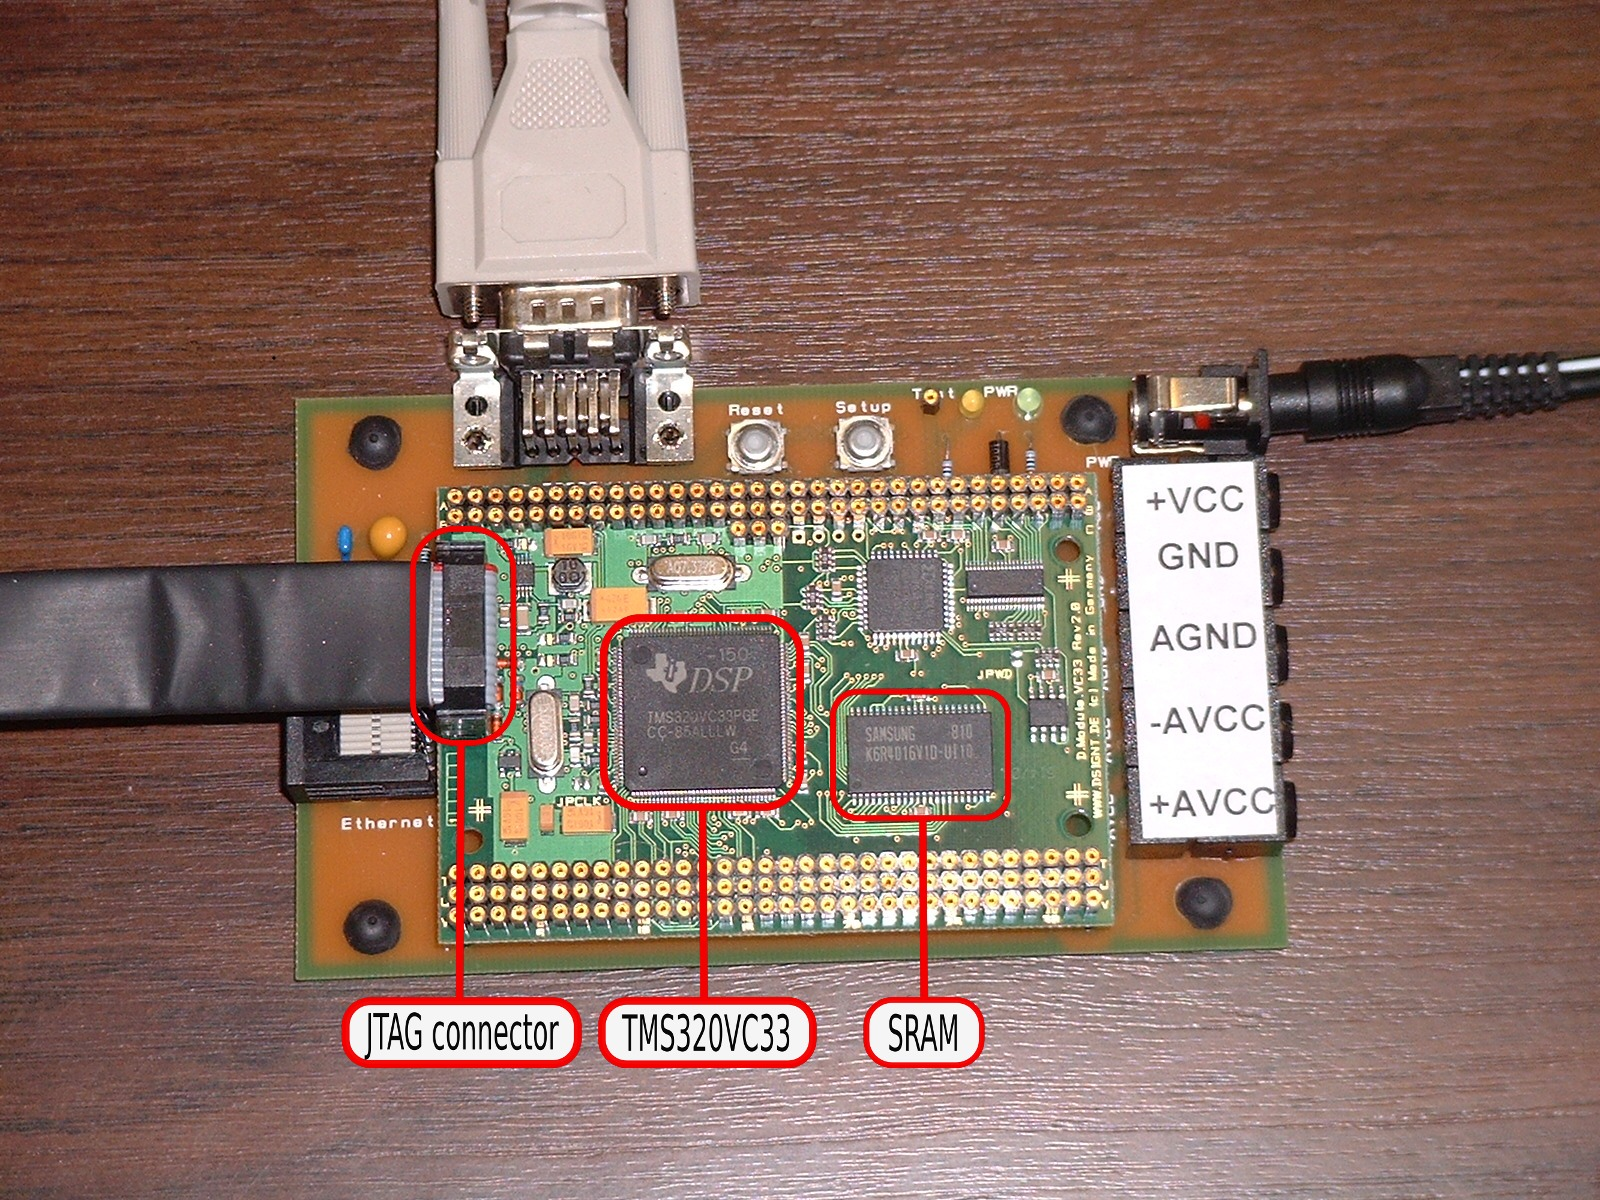
\includegraphics[width=7.0cm]{tms320c3x/fig_tms320c3x_board.jpg}
					\caption{\label{fig:tms320c3x_board} TMS320VC33 Board.}
				\end{center}
			\end{minipage}
			\begin{minipage}{8.0cm}
				\begin{center}
					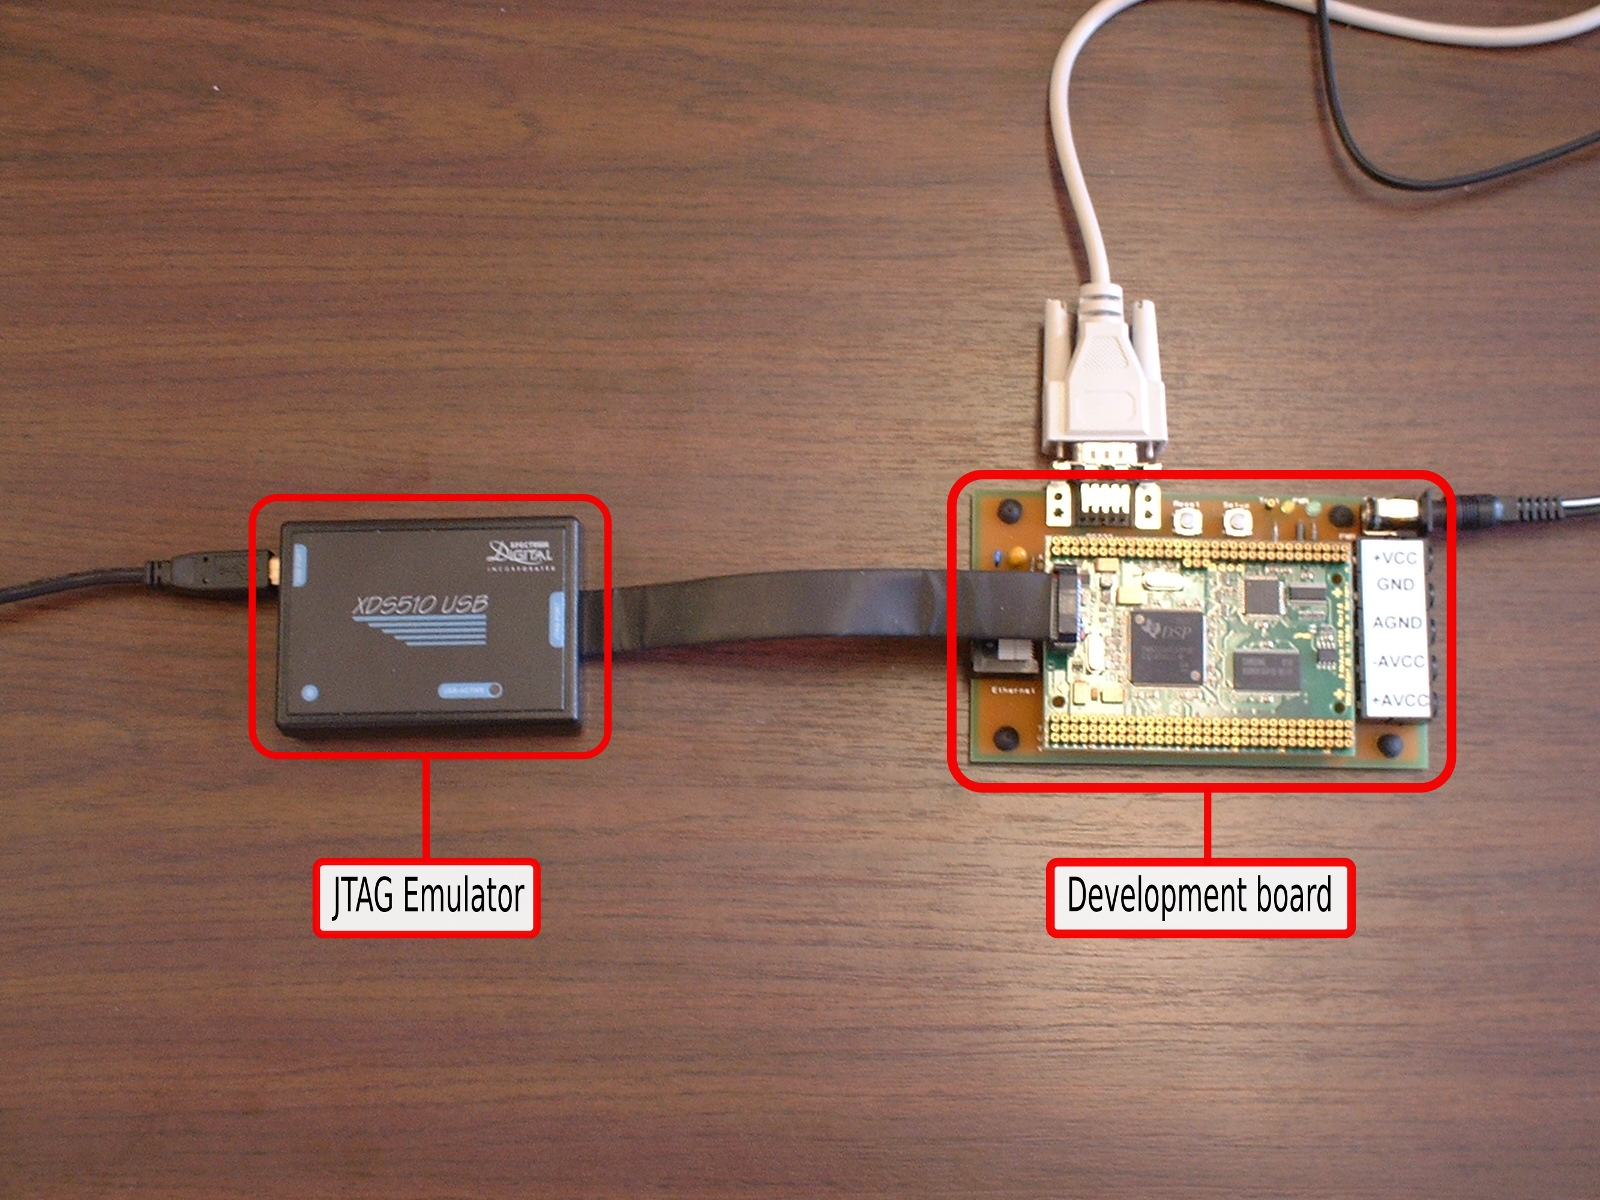
\includegraphics[width=7.0cm]{tms320c3x/fig_tms320c3x_dev_kit.jpg}
					\caption{\label{fig:tms320c3x_jtag_emu} TMS320VC33 board with JTAG.}
				\end{center}
			\end{minipage}
		\end{minipage}
	\end{center}
\end{figure}

The simulator validation involved using the TI C cross-compiler for Windows (see Section~\ref{tms320c3x_cross_compiler}) with the following versions:
\begin{itemize}
\item TMS320C3x/4x ANSI C Compiler Version 5.11
\item TMS320C3x/4x ANSI C Optimizer Version 5.13
\item TMS320C3x/4x ANSI C Code Generator Version 5.13
\item TMS320C3x/4x COFF Assembler Version 5.12
\item TMS320C3x/4x COFF Linker Version 5.11
\end{itemize}

The cross-compiler has generated COFF v2 files for TMS320C3X/C4X with little-endian headers matching the endianness of our building host machine (Windows XP x86).

\noindent The host machine configurations used to test both compilation and run of the simulator are:
\begin{itemize}
\item Redhat Linux RHEL4 x86/gcc 3.4.6 (32-bit little-endian machine)
\item Mandriva Linux 2009.1 x86/gcc 4.3.2 (32-bit little-endian machine)
\item Mandriva Linux 2010.0 x86/gcc 4.4.1 (32-bit little-endian machine)
\item Mageia Linux 3/gcc 4.7.2 (32-bit little-endian machine)
\item Ubuntu Linux 7.04 powerpc/gcc 4.1.2 (32-bit big-endian machine)
\item Ubuntu Linux 9.04 AMD64/x86\_64/gcc 4.3.3 (64-bit little-endian machine)
\item Ubuntu Linux 10.04 AMD64/x86\_64/gcc 4.4.3 (64-bit little-endian machine)
\item Mac OS X Leopard v10.5 x86/gcc 4.3.3 and gcc 4.4.2 (32-bit little-endian machine)
\item Windows XP x86/gcc mingw32 4.4.0 (32 bit little-endian machine)
\end{itemize}

Note that the UNISIM TMS320C3X has also been run under the control of \texttt{valgrind} (\url{http://valgrind.org}), a tool tracking memory related bugs such as memory leaks, unitialized memory reads, and control statements that depends on unitialized variables.

The following developement board (see Figures~\ref{fig:tms320c3x_board}~and~\ref{fig:tms320c3x_jtag_emu}) has been used to compare the simulator results against a real TMS320C3X DSP:
\begin{itemize}
\item A D.SignT DK.VC33-150-S2 development board
\item A D.SignT D.Module.VC33-150-S2 module including a TI TMS320VC33PGE (150 MFLOPS)
\item A 256K 32 bits SRAM with 1 Wait state
\item A 512K 8 bits Flash Memory
\item A Spectrum Digital XDS510USB JTAG Emulator
\item Code Composer IDE 4.10.36 SP2 C3X'C4X for Windows
\end{itemize}

The UNISIM TMS320C3X has been validated using integer benchmarks, floating point benchmarks, and unit tests of individual instructions.
These tests and benchmarks are available for download at \url{http://unisim-vp.org/site/download.html}.
The next sections provide details about the validation process.

\subsection{Benchmarks}
\label{tms320c3x_benchmarks}

This section presents the validation process of UNISIM TMS320C3X simulator using some application benchmarks.
For that purpose, several integer benchmarks have been ported from the MiBench benchmark suite to the TMS320C3X compiler tool chain.
The floating-point benchmarks have been extracted from the TMS320C3x DSK Software.
The following document has been used for selecting these floating-point benchmarks:
\begin{itemize}
\item \textit{TMS320C3x General Purpose Applications User's Guide} (SPRU194, January 1998)
\end{itemize}

These benchmarks have been run into the UNISIM TMS320C3X simulator using the application profiling capability of the inline debugger:
\begin{verbatim}
$ unisim-tms320c3x-2.0 -c sim_config.xml -s enable-inline-debugger=true
Loading xml parameters from: sim_config.xml
Parameters set using file "sim_config.xml"
....

....
loader: Loading symbol table
loader: Loading string table
ti-c-io: TI C I/O support is enabled
ti-c-io: Using __CIOBUF_ at 0xeac00 as I/O buffer
ti-c-io: Installing emulator breakpoint (SWI) for I/O at 0x2003c34 (symbol C$$IO$$)
ti-c-io: Installing emulator breakpoint (SWI) for EXIT at 0x20001cc (symbol C$$EXIT)
Starting simulation at system privilege level
0x00800048 <_c_int00>:
0x00800048:0x08700080 LDP @0x800000
inline-debugger> profile program on
inline-debugger> break C$$EXIT
inline-debugger> continue
...
0x00800073 <C$$EXIT>:
0x00800073:0x66000000 SWI
inline-debugger> profile program
0x00800000 <_enable_insn_cache>:1 times:0x08750800 LDI 2048, ST                                                                                                                                      
0x00800001 <.firm+0x1>:1 times:0x78800000 RETSU <@0x8012a9>                                                                                                                                          
....
0x00801279 <_fclose()+0x39>:3 times:0x0e240000 POP R4
0x0080127a <_fclose()+0x3a>:3 times:0x18740002 SUBI 2, SP
0x0080127b <_fclose()+0x3b>:3 times:0x68000001 BU R1 <_exit()+0x12>
inline-debugger> quit
\end{verbatim}

We extracted the instruction coverage from these applications profiles.
The table below shows the instruction coverage for each benchmark.
Benchmarks \texttt{Fibo}, \texttt{Quick sort}, \texttt{CRC32}, \texttt{Rijndael}, \texttt{Sha}, and \texttt{ADPCM} are integer benchmarks written in C.
Benchmarks \texttt{LP}, \texttt{BP}, \texttt{IIR}, and \texttt{FFT} are floating-point benchmarks written in C and assembly.
Each general addressing mode (see Table~\ref{table:tms320c3x_general_addressing_modes}) of each TMS320C3X instruction (see Tables~\ref{table:tms320c3x_load_store_instructions}, \ref{table:tms320c3x_interlocked_instructions},  \ref{table:tms320c3x_control_instructions}, \ref{table:tms320c3x_2ops_instructions}, \ref{table:tms320c3x_3ops_instructions}, \ref{table:tms320c3x_parallel_instructions} and \ref{table:tms320c3x_power_instructions}), actually has a row in the table.
A tick into a cell at the intersection of a row and a column indicates that the instruction of that row is covered by the benchmark of that column.

Although the integer benchmarks (written in C) have been selected to address the digital signal processing application domain, they have only validated the general operations of the simulator: program loading, program debugging, basic integer computation, control flow instructions, basic addressing modes \ldots
The reason of that limited validation scope is that the C compiler does not generate many different instructions and addressing modes among the integer benchmarks.
For instance, unusual addressing modes as the indirect addressing with circular modify and indirect addressing with bit reversed modify were not generated at all by the C compiler. 
Thus solely relying on these integer benchmarks for testing integer computation would have resulted in quite poor instruction coverage.
For instance, Instructions \texttt{addc}, \texttt{negb}, \texttt{rol}, \texttt{rolc}, \texttt{ror}, \texttt{rorc}, \texttt{subrb}, \texttt{addc3}, \texttt{subb3}, and most of parallel instructions but \texttt{ldi || ldi}, \texttt{ldi || sti}, and \texttt{sti || sti} were not covered at all.
Although the case of floating point benchmarks (written in C and assembly) is similar with an incomplete instruction coverage, the use of assembly has improved coverage of addressing modes and parallel instructions.
For instance, benchmarks \texttt{IIR} and \texttt{FFT} cover indirect addressing with circular modify and indirect addressing with bit reversed modify.
Nevertheless floating-point benchmarks insufficiently cover parallel instructions.
Particularly, Instructions \texttt{absf || stf}, \texttt{fix || sti}, \texttt{float || sti}, \texttt{negf || stf} were not covered at all.

\begin{center}
\tablehead{\hline
\multicolumn{1}{|c|}{\textbf{Instruction}} & \VROT{Fibonacci} & \VROT{Quick sort} & \VROT{CRC32} & \VROT{Rijndael} & \VROT{Sha} & \VROT{ADPCM coder} & \VROT{ADPCM decoder} & \VROT{DCT/Quantization} & \VROT{LP} & \VROT{BP} & \VROT{IIR} & \VROT{FFT}\\
\hline}
\tabletail{\hline}
\begin{supertabular}{|p{7.0cm}|p{0.35cm}|p{0.35cm}|p{0.35cm}|p{0.35cm}|p{0.35cm}|p{0.35cm}|p{0.35cm}|p{0.35cm}|p{0.35cm}|p{0.35cm}|p{0.35cm}|p{0.35cm}|}
\multicolumn{13}{|c|}{\textbf{lde}}\\
\hline
\multicolumn{1}{|p{7.0cm}|}{\scriptsize \texttt{lde reg, reg}} & \multicolumn{1}{p{0.35cm}|}{} & \multicolumn{1}{p{0.35cm}|}{} & \multicolumn{1}{p{0.35cm}|}{} & \multicolumn{1}{p{0.35cm}|}{} & \multicolumn{1}{p{0.35cm}|}{} & \multicolumn{1}{p{0.35cm}|}{} & \multicolumn{1}{p{0.35cm}|}{} & \multicolumn{1}{p{0.35cm}|}{} & \multicolumn{1}{p{0.35cm}|}{} & \multicolumn{1}{p{0.35cm}|}{} & \multicolumn{1}{p{0.35cm}|}{} & \multicolumn{1}{p{0.35cm}|}{\X}\\
\hline
\multicolumn{1}{|p{7.0cm}|}{\scriptsize \texttt{lde dir, reg}} & \multicolumn{1}{p{0.35cm}|}{} & \multicolumn{1}{p{0.35cm}|}{} & \multicolumn{1}{p{0.35cm}|}{} & \multicolumn{1}{p{0.35cm}|}{} & \multicolumn{1}{p{0.35cm}|}{} & \multicolumn{1}{p{0.35cm}|}{} & \multicolumn{1}{p{0.35cm}|}{} & \multicolumn{1}{p{0.35cm}|}{} & \multicolumn{1}{p{0.35cm}|}{} & \multicolumn{1}{p{0.35cm}|}{} & \multicolumn{1}{p{0.35cm}|}{} & \multicolumn{1}{p{0.35cm}|}{}\\
\hline
\multicolumn{1}{|p{7.0cm}|}{\scriptsize \texttt{lde indir, reg}} & \multicolumn{1}{p{0.35cm}|}{} & \multicolumn{1}{p{0.35cm}|}{} & \multicolumn{1}{p{0.35cm}|}{} & \multicolumn{1}{p{0.35cm}|}{} & \multicolumn{1}{p{0.35cm}|}{} & \multicolumn{1}{p{0.35cm}|}{} & \multicolumn{1}{p{0.35cm}|}{} & \multicolumn{1}{p{0.35cm}|}{} & \multicolumn{1}{p{0.35cm}|}{} & \multicolumn{1}{p{0.35cm}|}{} & \multicolumn{1}{p{0.35cm}|}{} & \multicolumn{1}{p{0.35cm}|}{}\\
\hline
\multicolumn{1}{|p{7.0cm}|}{\scriptsize \texttt{lde imm, reg}} & \multicolumn{1}{p{0.35cm}|}{} & \multicolumn{1}{p{0.35cm}|}{} & \multicolumn{1}{p{0.35cm}|}{} & \multicolumn{1}{p{0.35cm}|}{} & \multicolumn{1}{p{0.35cm}|}{} & \multicolumn{1}{p{0.35cm}|}{} & \multicolumn{1}{p{0.35cm}|}{} & \multicolumn{1}{p{0.35cm}|}{} & \multicolumn{1}{p{0.35cm}|}{} & \multicolumn{1}{p{0.35cm}|}{} & \multicolumn{1}{p{0.35cm}|}{} & \multicolumn{1}{p{0.35cm}|}{\X}\\
\hline
\multicolumn{13}{|c|}{\textbf{ldf}}\\
\hline
\multicolumn{1}{|p{7.0cm}|}{\scriptsize \texttt{ldf reg, reg}} & \multicolumn{1}{p{0.35cm}|}{} & \multicolumn{1}{p{0.35cm}|}{} & \multicolumn{1}{p{0.35cm}|}{} & \multicolumn{1}{p{0.35cm}|}{} & \multicolumn{1}{p{0.35cm}|}{} & \multicolumn{1}{p{0.35cm}|}{} & \multicolumn{1}{p{0.35cm}|}{} & \multicolumn{1}{p{0.35cm}|}{} & \multicolumn{1}{p{0.35cm}|}{} & \multicolumn{1}{p{0.35cm}|}{} & \multicolumn{1}{p{0.35cm}|}{\X} & \multicolumn{1}{p{0.35cm}|}{\X}\\
\hline
\multicolumn{1}{|p{7.0cm}|}{\scriptsize \texttt{ldf dir, reg}} & \multicolumn{1}{p{0.35cm}|}{} & \multicolumn{1}{p{0.35cm}|}{} & \multicolumn{1}{p{0.35cm}|}{} & \multicolumn{1}{p{0.35cm}|}{} & \multicolumn{1}{p{0.35cm}|}{} & \multicolumn{1}{p{0.35cm}|}{} & \multicolumn{1}{p{0.35cm}|}{} & \multicolumn{1}{p{0.35cm}|}{} & \multicolumn{1}{p{0.35cm}|}{} & \multicolumn{1}{p{0.35cm}|}{} & \multicolumn{1}{p{0.35cm}|}{} & \multicolumn{1}{p{0.35cm}|}{}\\
\hline
\multicolumn{1}{|p{7.0cm}|}{\scriptsize \texttt{ldf indir, reg}} & \multicolumn{1}{p{0.35cm}|}{} & \multicolumn{1}{p{0.35cm}|}{} & \multicolumn{1}{p{0.35cm}|}{} & \multicolumn{1}{p{0.35cm}|}{} & \multicolumn{1}{p{0.35cm}|}{} & \multicolumn{1}{p{0.35cm}|}{} & \multicolumn{1}{p{0.35cm}|}{} & \multicolumn{1}{p{0.35cm}|}{} & \multicolumn{1}{p{0.35cm}|}{\X} & \multicolumn{1}{p{0.35cm}|}{\X} & \multicolumn{1}{p{0.35cm}|}{\X} & \multicolumn{1}{p{0.35cm}|}{\X}\\
\hline
\multicolumn{1}{|p{7.0cm}|}{\scriptsize \texttt{ldf imm, reg}} & \multicolumn{1}{p{0.35cm}|}{} & \multicolumn{1}{p{0.35cm}|}{} & \multicolumn{1}{p{0.35cm}|}{} & \multicolumn{1}{p{0.35cm}|}{} & \multicolumn{1}{p{0.35cm}|}{} & \multicolumn{1}{p{0.35cm}|}{} & \multicolumn{1}{p{0.35cm}|}{} & \multicolumn{1}{p{0.35cm}|}{} & \multicolumn{1}{p{0.35cm}|}{\X} & \multicolumn{1}{p{0.35cm}|}{\X} & \multicolumn{1}{p{0.35cm}|}{} & \multicolumn{1}{p{0.35cm}|}{\X}\\
\hline
\multicolumn{13}{|c|}{\textbf{ldf\textit{cond}}}\\
\hline
\multicolumn{1}{|p{7.0cm}|}{\scriptsize \texttt{ldf\textit{cond} reg, reg}} & \multicolumn{1}{p{0.35cm}|}{} & \multicolumn{1}{p{0.35cm}|}{} & \multicolumn{1}{p{0.35cm}|}{} & \multicolumn{1}{p{0.35cm}|}{} & \multicolumn{1}{p{0.35cm}|}{} & \multicolumn{1}{p{0.35cm}|}{} & \multicolumn{1}{p{0.35cm}|}{} & \multicolumn{1}{p{0.35cm}|}{} & \multicolumn{1}{p{0.35cm}|}{\X} & \multicolumn{1}{p{0.35cm}|}{\X} & \multicolumn{1}{p{0.35cm}|}{\X} & \multicolumn{1}{p{0.35cm}|}{\X}\\
\hline
\multicolumn{1}{|p{7.0cm}|}{\scriptsize \texttt{ldf\textit{cond} dir, reg}} & \multicolumn{1}{p{0.35cm}|}{} & \multicolumn{1}{p{0.35cm}|}{} & \multicolumn{1}{p{0.35cm}|}{} & \multicolumn{1}{p{0.35cm}|}{} & \multicolumn{1}{p{0.35cm}|}{} & \multicolumn{1}{p{0.35cm}|}{} & \multicolumn{1}{p{0.35cm}|}{} & \multicolumn{1}{p{0.35cm}|}{} & \multicolumn{1}{p{0.35cm}|}{\X} & \multicolumn{1}{p{0.35cm}|}{\X} & \multicolumn{1}{p{0.35cm}|}{\X} & \multicolumn{1}{p{0.35cm}|}{\X}\\
\hline
\multicolumn{1}{|p{7.0cm}|}{\scriptsize \texttt{ldf\textit{cond} indir, reg}} & \multicolumn{1}{p{0.35cm}|}{} & \multicolumn{1}{p{0.35cm}|}{} & \multicolumn{1}{p{0.35cm}|}{} & \multicolumn{1}{p{0.35cm}|}{} & \multicolumn{1}{p{0.35cm}|}{} & \multicolumn{1}{p{0.35cm}|}{} & \multicolumn{1}{p{0.35cm}|}{} & \multicolumn{1}{p{0.35cm}|}{} & \multicolumn{1}{p{0.35cm}|}{} & \multicolumn{1}{p{0.35cm}|}{\X} & \multicolumn{1}{p{0.35cm}|}{\X} & \multicolumn{1}{p{0.35cm}|}{\X}\\
\hline
\multicolumn{1}{|p{7.0cm}|}{\scriptsize \texttt{ldf\textit{cond} imm, reg}} & \multicolumn{1}{p{0.35cm}|}{} & \multicolumn{1}{p{0.35cm}|}{} & \multicolumn{1}{p{0.35cm}|}{} & \multicolumn{1}{p{0.35cm}|}{} & \multicolumn{1}{p{0.35cm}|}{} & \multicolumn{1}{p{0.35cm}|}{} & \multicolumn{1}{p{0.35cm}|}{} & \multicolumn{1}{p{0.35cm}|}{} & \multicolumn{1}{p{0.35cm}|}{\X} & \multicolumn{1}{p{0.35cm}|}{\X} & \multicolumn{1}{p{0.35cm}|}{\X} & \multicolumn{1}{p{0.35cm}|}{\X}\\
\hline
\multicolumn{13}{|c|}{\textbf{ldi}}\\
\hline
\multicolumn{1}{|p{7.0cm}|}{\scriptsize \texttt{ldi reg, reg}} & \multicolumn{1}{p{0.35cm}|}{\X} & \multicolumn{1}{p{0.35cm}|}{\X} & \multicolumn{1}{p{0.35cm}|}{\X} & \multicolumn{1}{p{0.35cm}|}{\X} & \multicolumn{1}{p{0.35cm}|}{\X} & \multicolumn{1}{p{0.35cm}|}{\X} & \multicolumn{1}{p{0.35cm}|}{\X} & \multicolumn{1}{p{0.35cm}|}{\X} & \multicolumn{1}{p{0.35cm}|}{\X} & \multicolumn{1}{p{0.35cm}|}{} & \multicolumn{1}{p{0.35cm}|}{\X} & \multicolumn{1}{p{0.35cm}|}{\X}\\
\hline
\multicolumn{1}{|p{7.0cm}|}{\scriptsize \texttt{ldi dir, reg}} & \multicolumn{1}{p{0.35cm}|}{\X} & \multicolumn{1}{p{0.35cm}|}{\X} & \multicolumn{1}{p{0.35cm}|}{\X} & \multicolumn{1}{p{0.35cm}|}{\X} & \multicolumn{1}{p{0.35cm}|}{\X} & \multicolumn{1}{p{0.35cm}|}{\X} & \multicolumn{1}{p{0.35cm}|}{\X} & \multicolumn{1}{p{0.35cm}|}{\X} & \multicolumn{1}{p{0.35cm}|}{\X} & \multicolumn{1}{p{0.35cm}|}{\X} & \multicolumn{1}{p{0.35cm}|}{\X} & \multicolumn{1}{p{0.35cm}|}{\X}\\
\hline
\multicolumn{1}{|p{7.0cm}|}{\scriptsize \texttt{ldi indir, reg}} & \multicolumn{1}{p{0.35cm}|}{} & \multicolumn{1}{p{0.35cm}|}{\X} & \multicolumn{1}{p{0.35cm}|}{\X} & \multicolumn{1}{p{0.35cm}|}{\X} & \multicolumn{1}{p{0.35cm}|}{\X} & \multicolumn{1}{p{0.35cm}|}{\X} & \multicolumn{1}{p{0.35cm}|}{\X} & \multicolumn{1}{p{0.35cm}|}{} & \multicolumn{1}{p{0.35cm}|}{\X} & \multicolumn{1}{p{0.35cm}|}{\X} & \multicolumn{1}{p{0.35cm}|}{\X} & \multicolumn{1}{p{0.35cm}|}{\X}\\
\hline
\multicolumn{1}{|p{7.0cm}|}{\scriptsize \texttt{ldi imm, reg}} & \multicolumn{1}{p{0.35cm}|}{\X} & \multicolumn{1}{p{0.35cm}|}{\X} & \multicolumn{1}{p{0.35cm}|}{\X} & \multicolumn{1}{p{0.35cm}|}{\X} & \multicolumn{1}{p{0.35cm}|}{\X} & \multicolumn{1}{p{0.35cm}|}{\X} & \multicolumn{1}{p{0.35cm}|}{\X} & \multicolumn{1}{p{0.35cm}|}{\X} & \multicolumn{1}{p{0.35cm}|}{\X} & \multicolumn{1}{p{0.35cm}|}{} & \multicolumn{1}{p{0.35cm}|}{\X} & \multicolumn{1}{p{0.35cm}|}{\X}\\
\hline
\multicolumn{13}{|c|}{\textbf{ldi\textit{cond}}}\\
\hline
\multicolumn{1}{|p{7.0cm}|}{\scriptsize \texttt{ldi\textit{cond} reg, reg}} & \multicolumn{1}{p{0.35cm}|}{\X} & \multicolumn{1}{p{0.35cm}|}{\X} & \multicolumn{1}{p{0.35cm}|}{\X} & \multicolumn{1}{p{0.35cm}|}{\X} & \multicolumn{1}{p{0.35cm}|}{\X} & \multicolumn{1}{p{0.35cm}|}{\X} & \multicolumn{1}{p{0.35cm}|}{\X} & \multicolumn{1}{p{0.35cm}|}{\X} & \multicolumn{1}{p{0.35cm}|}{\X} & \multicolumn{1}{p{0.35cm}|}{\X} & \multicolumn{1}{p{0.35cm}|}{\X} & \multicolumn{1}{p{0.35cm}|}{\X}\\
\hline
\multicolumn{1}{|p{7.0cm}|}{\scriptsize \texttt{ldi\textit{cond} dir, reg}} & \multicolumn{1}{p{0.35cm}|}{\X} & \multicolumn{1}{p{0.35cm}|}{\X} & \multicolumn{1}{p{0.35cm}|}{\X} & \multicolumn{1}{p{0.35cm}|}{\X} & \multicolumn{1}{p{0.35cm}|}{\X} & \multicolumn{1}{p{0.35cm}|}{\X} & \multicolumn{1}{p{0.35cm}|}{\X} & \multicolumn{1}{p{0.35cm}|}{\X} & \multicolumn{1}{p{0.35cm}|}{\X} & \multicolumn{1}{p{0.35cm}|}{\X} & \multicolumn{1}{p{0.35cm}|}{\X} & \multicolumn{1}{p{0.35cm}|}{\X}\\
\hline
\multicolumn{1}{|p{7.0cm}|}{\scriptsize \texttt{ldi\textit{cond} indir, reg}} & \multicolumn{1}{p{0.35cm}|}{\X} & \multicolumn{1}{p{0.35cm}|}{\X} & \multicolumn{1}{p{0.35cm}|}{\X} & \multicolumn{1}{p{0.35cm}|}{\X} & \multicolumn{1}{p{0.35cm}|}{\X} & \multicolumn{1}{p{0.35cm}|}{\X} & \multicolumn{1}{p{0.35cm}|}{\X} & \multicolumn{1}{p{0.35cm}|}{\X} & \multicolumn{1}{p{0.35cm}|}{\X} & \multicolumn{1}{p{0.35cm}|}{\X} & \multicolumn{1}{p{0.35cm}|}{\X} & \multicolumn{1}{p{0.35cm}|}{\X}\\
\hline
\multicolumn{1}{|p{7.0cm}|}{\scriptsize \texttt{ldi\textit{cond} imm, reg}} & \multicolumn{1}{p{0.35cm}|}{\X} & \multicolumn{1}{p{0.35cm}|}{\X} & \multicolumn{1}{p{0.35cm}|}{\X} & \multicolumn{1}{p{0.35cm}|}{\X} & \multicolumn{1}{p{0.35cm}|}{\X} & \multicolumn{1}{p{0.35cm}|}{\X} & \multicolumn{1}{p{0.35cm}|}{\X} & \multicolumn{1}{p{0.35cm}|}{\X} & \multicolumn{1}{p{0.35cm}|}{\X} & \multicolumn{1}{p{0.35cm}|}{\X} & \multicolumn{1}{p{0.35cm}|}{\X} & \multicolumn{1}{p{0.35cm}|}{\X}\\
\hline
\multicolumn{13}{|c|}{\textbf{ldm}}\\
\hline
\multicolumn{1}{|p{7.0cm}|}{\scriptsize \texttt{ldm reg, reg}} & \multicolumn{1}{p{0.35cm}|}{} & \multicolumn{1}{p{0.35cm}|}{} & \multicolumn{1}{p{0.35cm}|}{} & \multicolumn{1}{p{0.35cm}|}{} & \multicolumn{1}{p{0.35cm}|}{} & \multicolumn{1}{p{0.35cm}|}{} & \multicolumn{1}{p{0.35cm}|}{} & \multicolumn{1}{p{0.35cm}|}{} & \multicolumn{1}{p{0.35cm}|}{} & \multicolumn{1}{p{0.35cm}|}{} & \multicolumn{1}{p{0.35cm}|}{} & \multicolumn{1}{p{0.35cm}|}{}\\
\hline
\multicolumn{1}{|p{7.0cm}|}{\scriptsize \texttt{ldm dir, reg}} & \multicolumn{1}{p{0.35cm}|}{} & \multicolumn{1}{p{0.35cm}|}{} & \multicolumn{1}{p{0.35cm}|}{} & \multicolumn{1}{p{0.35cm}|}{} & \multicolumn{1}{p{0.35cm}|}{} & \multicolumn{1}{p{0.35cm}|}{} & \multicolumn{1}{p{0.35cm}|}{} & \multicolumn{1}{p{0.35cm}|}{} & \multicolumn{1}{p{0.35cm}|}{} & \multicolumn{1}{p{0.35cm}|}{} & \multicolumn{1}{p{0.35cm}|}{} & \multicolumn{1}{p{0.35cm}|}{}\\
\hline
\multicolumn{1}{|p{7.0cm}|}{\scriptsize \texttt{ldm indir, reg}} & \multicolumn{1}{p{0.35cm}|}{} & \multicolumn{1}{p{0.35cm}|}{} & \multicolumn{1}{p{0.35cm}|}{} & \multicolumn{1}{p{0.35cm}|}{} & \multicolumn{1}{p{0.35cm}|}{} & \multicolumn{1}{p{0.35cm}|}{} & \multicolumn{1}{p{0.35cm}|}{} & \multicolumn{1}{p{0.35cm}|}{} & \multicolumn{1}{p{0.35cm}|}{} & \multicolumn{1}{p{0.35cm}|}{} & \multicolumn{1}{p{0.35cm}|}{} & \multicolumn{1}{p{0.35cm}|}{}\\
\hline
\multicolumn{1}{|p{7.0cm}|}{\scriptsize \texttt{ldm imm, reg}} & \multicolumn{1}{p{0.35cm}|}{} & \multicolumn{1}{p{0.35cm}|}{} & \multicolumn{1}{p{0.35cm}|}{} & \multicolumn{1}{p{0.35cm}|}{} & \multicolumn{1}{p{0.35cm}|}{} & \multicolumn{1}{p{0.35cm}|}{} & \multicolumn{1}{p{0.35cm}|}{} & \multicolumn{1}{p{0.35cm}|}{} & \multicolumn{1}{p{0.35cm}|}{} & \multicolumn{1}{p{0.35cm}|}{} & \multicolumn{1}{p{0.35cm}|}{} & \multicolumn{1}{p{0.35cm}|}{\X}\\
\hline
\multicolumn{13}{|c|}{\textbf{ldp}}\\
\hline
\multicolumn{1}{|p{7.0cm}|}{\scriptsize \texttt{ldp src}} & \multicolumn{1}{p{0.35cm}|}{\X} & \multicolumn{1}{p{0.35cm}|}{\X} & \multicolumn{1}{p{0.35cm}|}{\X} & \multicolumn{1}{p{0.35cm}|}{\X} & \multicolumn{1}{p{0.35cm}|}{\X} & \multicolumn{1}{p{0.35cm}|}{\X} & \multicolumn{1}{p{0.35cm}|}{\X} & \multicolumn{1}{p{0.35cm}|}{\X} & \multicolumn{1}{p{0.35cm}|}{\X} & \multicolumn{1}{p{0.35cm}|}{\X} & \multicolumn{1}{p{0.35cm}|}{\X} & \multicolumn{1}{p{0.35cm}|}{\X}\\
\hline
\multicolumn{13}{|c|}{\textbf{pop}}\\
\hline
\multicolumn{1}{|p{7.0cm}|}{\scriptsize \texttt{pop reg}} & \multicolumn{1}{p{0.35cm}|}{\X} & \multicolumn{1}{p{0.35cm}|}{\X} & \multicolumn{1}{p{0.35cm}|}{\X} & \multicolumn{1}{p{0.35cm}|}{\X} & \multicolumn{1}{p{0.35cm}|}{\X} & \multicolumn{1}{p{0.35cm}|}{\X} & \multicolumn{1}{p{0.35cm}|}{\X} & \multicolumn{1}{p{0.35cm}|}{\X} & \multicolumn{1}{p{0.35cm}|}{\X} & \multicolumn{1}{p{0.35cm}|}{\X} & \multicolumn{1}{p{0.35cm}|}{\X} & \multicolumn{1}{p{0.35cm}|}{\X}\\
\hline
\multicolumn{13}{|c|}{\textbf{popf}}\\
\hline
\multicolumn{1}{|p{7.0cm}|}{\scriptsize \texttt{popf reg}} & \multicolumn{1}{p{0.35cm}|}{} & \multicolumn{1}{p{0.35cm}|}{} & \multicolumn{1}{p{0.35cm}|}{} & \multicolumn{1}{p{0.35cm}|}{\X} & \multicolumn{1}{p{0.35cm}|}{\X} & \multicolumn{1}{p{0.35cm}|}{\X} & \multicolumn{1}{p{0.35cm}|}{\X} & \multicolumn{1}{p{0.35cm}|}{\X} & \multicolumn{1}{p{0.35cm}|}{\X} & \multicolumn{1}{p{0.35cm}|}{\X} & \multicolumn{1}{p{0.35cm}|}{\X} & \multicolumn{1}{p{0.35cm}|}{\X}\\
\hline
\multicolumn{13}{|c|}{\textbf{push}}\\
\hline
\multicolumn{1}{|p{7.0cm}|}{\scriptsize \texttt{push reg}} & \multicolumn{1}{p{0.35cm}|}{\X} & \multicolumn{1}{p{0.35cm}|}{\X} & \multicolumn{1}{p{0.35cm}|}{\X} & \multicolumn{1}{p{0.35cm}|}{\X} & \multicolumn{1}{p{0.35cm}|}{\X} & \multicolumn{1}{p{0.35cm}|}{\X} & \multicolumn{1}{p{0.35cm}|}{\X} & \multicolumn{1}{p{0.35cm}|}{\X} & \multicolumn{1}{p{0.35cm}|}{\X} & \multicolumn{1}{p{0.35cm}|}{\X} & \multicolumn{1}{p{0.35cm}|}{\X} & \multicolumn{1}{p{0.35cm}|}{\X}\\
\hline
\multicolumn{13}{|c|}{\textbf{pushf}}\\
\hline
\multicolumn{1}{|p{7.0cm}|}{\scriptsize \texttt{pushf reg}} & \multicolumn{1}{p{0.35cm}|}{\X} & \multicolumn{1}{p{0.35cm}|}{\X} & \multicolumn{1}{p{0.35cm}|}{\X} & \multicolumn{1}{p{0.35cm}|}{\X} & \multicolumn{1}{p{0.35cm}|}{\X} & \multicolumn{1}{p{0.35cm}|}{\X} & \multicolumn{1}{p{0.35cm}|}{\X} & \multicolumn{1}{p{0.35cm}|}{\X} & \multicolumn{1}{p{0.35cm}|}{\X} & \multicolumn{1}{p{0.35cm}|}{\X} & \multicolumn{1}{p{0.35cm}|}{\X} & \multicolumn{1}{p{0.35cm}|}{\X}\\
\hline
\multicolumn{13}{|c|}{\textbf{stf}}\\
\hline
\multicolumn{1}{|p{7.0cm}|}{\scriptsize \texttt{stf reg, dir}} & \multicolumn{1}{p{0.35cm}|}{} & \multicolumn{1}{p{0.35cm}|}{} & \multicolumn{1}{p{0.35cm}|}{} & \multicolumn{1}{p{0.35cm}|}{} & \multicolumn{1}{p{0.35cm}|}{} & \multicolumn{1}{p{0.35cm}|}{} & \multicolumn{1}{p{0.35cm}|}{} & \multicolumn{1}{p{0.35cm}|}{} & \multicolumn{1}{p{0.35cm}|}{} & \multicolumn{1}{p{0.35cm}|}{} & \multicolumn{1}{p{0.35cm}|}{\X} & \multicolumn{1}{p{0.35cm}|}{}\\
\hline
\multicolumn{1}{|p{7.0cm}|}{\scriptsize \texttt{stf reg, indir}} & \multicolumn{1}{p{0.35cm}|}{} & \multicolumn{1}{p{0.35cm}|}{} & \multicolumn{1}{p{0.35cm}|}{} & \multicolumn{1}{p{0.35cm}|}{} & \multicolumn{1}{p{0.35cm}|}{} & \multicolumn{1}{p{0.35cm}|}{} & \multicolumn{1}{p{0.35cm}|}{} & \multicolumn{1}{p{0.35cm}|}{} & \multicolumn{1}{p{0.35cm}|}{\X} & \multicolumn{1}{p{0.35cm}|}{\X} & \multicolumn{1}{p{0.35cm}|}{\X} & \multicolumn{1}{p{0.35cm}|}{\X}\\
\hline
\multicolumn{13}{|c|}{\textbf{sti}}\\
\hline
\multicolumn{1}{|p{7.0cm}|}{\scriptsize \texttt{sti reg, dir}} & \multicolumn{1}{p{0.35cm}|}{\X} & \multicolumn{1}{p{0.35cm}|}{\X} & \multicolumn{1}{p{0.35cm}|}{\X} & \multicolumn{1}{p{0.35cm}|}{\X} & \multicolumn{1}{p{0.35cm}|}{\X} & \multicolumn{1}{p{0.35cm}|}{\X} & \multicolumn{1}{p{0.35cm}|}{\X} & \multicolumn{1}{p{0.35cm}|}{\X} & \multicolumn{1}{p{0.35cm}|}{\X} & \multicolumn{1}{p{0.35cm}|}{\X} & \multicolumn{1}{p{0.35cm}|}{\X} & \multicolumn{1}{p{0.35cm}|}{\X}\\
\hline
\multicolumn{1}{|p{7.0cm}|}{\scriptsize \texttt{sti reg, indir}} & \multicolumn{1}{p{0.35cm}|}{\X} & \multicolumn{1}{p{0.35cm}|}{\X} & \multicolumn{1}{p{0.35cm}|}{\X} & \multicolumn{1}{p{0.35cm}|}{\X} & \multicolumn{1}{p{0.35cm}|}{\X} & \multicolumn{1}{p{0.35cm}|}{\X} & \multicolumn{1}{p{0.35cm}|}{\X} & \multicolumn{1}{p{0.35cm}|}{\X} & \multicolumn{1}{p{0.35cm}|}{\X} & \multicolumn{1}{p{0.35cm}|}{\X} & \multicolumn{1}{p{0.35cm}|}{\X} & \multicolumn{1}{p{0.35cm}|}{\X}\\
\hline
\multicolumn{13}{|c|}{\textbf{ldfi}}\\
\hline
\multicolumn{1}{|p{7.0cm}|}{\scriptsize \texttt{ldfi dir, reg}} & \multicolumn{1}{p{0.35cm}|}{} & \multicolumn{1}{p{0.35cm}|}{} & \multicolumn{1}{p{0.35cm}|}{} & \multicolumn{1}{p{0.35cm}|}{} & \multicolumn{1}{p{0.35cm}|}{} & \multicolumn{1}{p{0.35cm}|}{} & \multicolumn{1}{p{0.35cm}|}{} & \multicolumn{1}{p{0.35cm}|}{} & \multicolumn{1}{p{0.35cm}|}{} & \multicolumn{1}{p{0.35cm}|}{} & \multicolumn{1}{p{0.35cm}|}{} & \multicolumn{1}{p{0.35cm}|}{}\\
\hline
\multicolumn{1}{|p{7.0cm}|}{\scriptsize \texttt{ldfi indir, reg}} & \multicolumn{1}{p{0.35cm}|}{} & \multicolumn{1}{p{0.35cm}|}{} & \multicolumn{1}{p{0.35cm}|}{} & \multicolumn{1}{p{0.35cm}|}{} & \multicolumn{1}{p{0.35cm}|}{} & \multicolumn{1}{p{0.35cm}|}{} & \multicolumn{1}{p{0.35cm}|}{} & \multicolumn{1}{p{0.35cm}|}{} & \multicolumn{1}{p{0.35cm}|}{} & \multicolumn{1}{p{0.35cm}|}{} & \multicolumn{1}{p{0.35cm}|}{} & \multicolumn{1}{p{0.35cm}|}{}\\
\hline
\multicolumn{13}{|c|}{\textbf{ldii}}\\
\hline
\multicolumn{1}{|p{7.0cm}|}{\scriptsize \texttt{ldii dir, reg}} & \multicolumn{1}{p{0.35cm}|}{} & \multicolumn{1}{p{0.35cm}|}{} & \multicolumn{1}{p{0.35cm}|}{} & \multicolumn{1}{p{0.35cm}|}{} & \multicolumn{1}{p{0.35cm}|}{} & \multicolumn{1}{p{0.35cm}|}{} & \multicolumn{1}{p{0.35cm}|}{} & \multicolumn{1}{p{0.35cm}|}{} & \multicolumn{1}{p{0.35cm}|}{} & \multicolumn{1}{p{0.35cm}|}{} & \multicolumn{1}{p{0.35cm}|}{} & \multicolumn{1}{p{0.35cm}|}{}\\
\hline
\multicolumn{1}{|p{7.0cm}|}{\scriptsize \texttt{ldii indir, reg}} & \multicolumn{1}{p{0.35cm}|}{} & \multicolumn{1}{p{0.35cm}|}{} & \multicolumn{1}{p{0.35cm}|}{} & \multicolumn{1}{p{0.35cm}|}{} & \multicolumn{1}{p{0.35cm}|}{} & \multicolumn{1}{p{0.35cm}|}{} & \multicolumn{1}{p{0.35cm}|}{} & \multicolumn{1}{p{0.35cm}|}{} & \multicolumn{1}{p{0.35cm}|}{} & \multicolumn{1}{p{0.35cm}|}{} & \multicolumn{1}{p{0.35cm}|}{} & \multicolumn{1}{p{0.35cm}|}{}\\
\hline
\multicolumn{13}{|c|}{\textbf{sigi}}\\
\hline
\multicolumn{1}{|p{7.0cm}|}{\scriptsize \texttt{sigi}} & \multicolumn{1}{p{0.35cm}|}{} & \multicolumn{1}{p{0.35cm}|}{} & \multicolumn{1}{p{0.35cm}|}{} & \multicolumn{1}{p{0.35cm}|}{} & \multicolumn{1}{p{0.35cm}|}{} & \multicolumn{1}{p{0.35cm}|}{} & \multicolumn{1}{p{0.35cm}|}{} & \multicolumn{1}{p{0.35cm}|}{} & \multicolumn{1}{p{0.35cm}|}{} & \multicolumn{1}{p{0.35cm}|}{} & \multicolumn{1}{p{0.35cm}|}{} & \multicolumn{1}{p{0.35cm}|}{}\\
\hline
\multicolumn{13}{|c|}{\textbf{stfi}}\\
\hline
\multicolumn{1}{|p{7.0cm}|}{\scriptsize \texttt{stfi reg, dir}} & \multicolumn{1}{p{0.35cm}|}{} & \multicolumn{1}{p{0.35cm}|}{} & \multicolumn{1}{p{0.35cm}|}{} & \multicolumn{1}{p{0.35cm}|}{} & \multicolumn{1}{p{0.35cm}|}{} & \multicolumn{1}{p{0.35cm}|}{} & \multicolumn{1}{p{0.35cm}|}{} & \multicolumn{1}{p{0.35cm}|}{} & \multicolumn{1}{p{0.35cm}|}{} & \multicolumn{1}{p{0.35cm}|}{} & \multicolumn{1}{p{0.35cm}|}{} & \multicolumn{1}{p{0.35cm}|}{}\\
\hline
\multicolumn{1}{|p{7.0cm}|}{\scriptsize \texttt{stfi reg, indir}} & \multicolumn{1}{p{0.35cm}|}{} & \multicolumn{1}{p{0.35cm}|}{} & \multicolumn{1}{p{0.35cm}|}{} & \multicolumn{1}{p{0.35cm}|}{} & \multicolumn{1}{p{0.35cm}|}{} & \multicolumn{1}{p{0.35cm}|}{} & \multicolumn{1}{p{0.35cm}|}{} & \multicolumn{1}{p{0.35cm}|}{} & \multicolumn{1}{p{0.35cm}|}{} & \multicolumn{1}{p{0.35cm}|}{} & \multicolumn{1}{p{0.35cm}|}{} & \multicolumn{1}{p{0.35cm}|}{}\\
\hline
\multicolumn{13}{|c|}{\textbf{stii}}\\
\hline
\multicolumn{1}{|p{7.0cm}|}{\scriptsize \texttt{stii reg, dir}} & \multicolumn{1}{p{0.35cm}|}{} & \multicolumn{1}{p{0.35cm}|}{} & \multicolumn{1}{p{0.35cm}|}{} & \multicolumn{1}{p{0.35cm}|}{} & \multicolumn{1}{p{0.35cm}|}{} & \multicolumn{1}{p{0.35cm}|}{} & \multicolumn{1}{p{0.35cm}|}{} & \multicolumn{1}{p{0.35cm}|}{} & \multicolumn{1}{p{0.35cm}|}{} & \multicolumn{1}{p{0.35cm}|}{} & \multicolumn{1}{p{0.35cm}|}{} & \multicolumn{1}{p{0.35cm}|}{}\\
\hline
\multicolumn{1}{|p{7.0cm}|}{\scriptsize \texttt{stii reg, indir}} & \multicolumn{1}{p{0.35cm}|}{} & \multicolumn{1}{p{0.35cm}|}{} & \multicolumn{1}{p{0.35cm}|}{} & \multicolumn{1}{p{0.35cm}|}{} & \multicolumn{1}{p{0.35cm}|}{} & \multicolumn{1}{p{0.35cm}|}{} & \multicolumn{1}{p{0.35cm}|}{} & \multicolumn{1}{p{0.35cm}|}{} & \multicolumn{1}{p{0.35cm}|}{} & \multicolumn{1}{p{0.35cm}|}{} & \multicolumn{1}{p{0.35cm}|}{} & \multicolumn{1}{p{0.35cm}|}{}\\
\hline
\multicolumn{13}{|c|}{\textbf{b\textit{cond}}}\\
\hline
\multicolumn{1}{|p{7.0cm}|}{\scriptsize \texttt{b\textit{cond} reg}} & \multicolumn{1}{p{0.35cm}|}{\X} & \multicolumn{1}{p{0.35cm}|}{\X} & \multicolumn{1}{p{0.35cm}|}{\X} & \multicolumn{1}{p{0.35cm}|}{\X} & \multicolumn{1}{p{0.35cm}|}{\X} & \multicolumn{1}{p{0.35cm}|}{\X} & \multicolumn{1}{p{0.35cm}|}{\X} & \multicolumn{1}{p{0.35cm}|}{\X} & \multicolumn{1}{p{0.35cm}|}{} & \multicolumn{1}{p{0.35cm}|}{} & \multicolumn{1}{p{0.35cm}|}{} & \multicolumn{1}{p{0.35cm}|}{\X}\\
\hline
\multicolumn{1}{|p{7.0cm}|}{\scriptsize \texttt{b\textit{cond} disp}} & \multicolumn{1}{p{0.35cm}|}{\X} & \multicolumn{1}{p{0.35cm}|}{\X} & \multicolumn{1}{p{0.35cm}|}{\X} & \multicolumn{1}{p{0.35cm}|}{\X} & \multicolumn{1}{p{0.35cm}|}{\X} & \multicolumn{1}{p{0.35cm}|}{\X} & \multicolumn{1}{p{0.35cm}|}{\X} & \multicolumn{1}{p{0.35cm}|}{\X} & \multicolumn{1}{p{0.35cm}|}{\X} & \multicolumn{1}{p{0.35cm}|}{\X} & \multicolumn{1}{p{0.35cm}|}{\X} & \multicolumn{1}{p{0.35cm}|}{\X}\\
\hline
\multicolumn{13}{|c|}{\textbf{b\textit{cond}d}}\\
\hline
\multicolumn{1}{|p{7.0cm}|}{\scriptsize \texttt{b\textit{cond}d reg}} & \multicolumn{1}{p{0.35cm}|}{\X} & \multicolumn{1}{p{0.35cm}|}{\X} & \multicolumn{1}{p{0.35cm}|}{\X} & \multicolumn{1}{p{0.35cm}|}{\X} & \multicolumn{1}{p{0.35cm}|}{\X} & \multicolumn{1}{p{0.35cm}|}{\X} & \multicolumn{1}{p{0.35cm}|}{\X} & \multicolumn{1}{p{0.35cm}|}{\X} & \multicolumn{1}{p{0.35cm}|}{} & \multicolumn{1}{p{0.35cm}|}{} & \multicolumn{1}{p{0.35cm}|}{} & \multicolumn{1}{p{0.35cm}|}{\X}\\
\hline
\multicolumn{1}{|p{7.0cm}|}{\scriptsize \texttt{b\textit{cond}d disp}} & \multicolumn{1}{p{0.35cm}|}{\X} & \multicolumn{1}{p{0.35cm}|}{\X} & \multicolumn{1}{p{0.35cm}|}{\X} & \multicolumn{1}{p{0.35cm}|}{\X} & \multicolumn{1}{p{0.35cm}|}{\X} & \multicolumn{1}{p{0.35cm}|}{\X} & \multicolumn{1}{p{0.35cm}|}{\X} & \multicolumn{1}{p{0.35cm}|}{\X} & \multicolumn{1}{p{0.35cm}|}{\X} & \multicolumn{1}{p{0.35cm}|}{\X} & \multicolumn{1}{p{0.35cm}|}{\X} & \multicolumn{1}{p{0.35cm}|}{\X}\\
\hline
\multicolumn{13}{|c|}{\textbf{br}}\\
\hline
\multicolumn{1}{|p{7.0cm}|}{\scriptsize \texttt{br src}} & \multicolumn{1}{p{0.35cm}|}{} & \multicolumn{1}{p{0.35cm}|}{} & \multicolumn{1}{p{0.35cm}|}{} & \multicolumn{1}{p{0.35cm}|}{} & \multicolumn{1}{p{0.35cm}|}{} & \multicolumn{1}{p{0.35cm}|}{} & \multicolumn{1}{p{0.35cm}|}{} & \multicolumn{1}{p{0.35cm}|}{} & \multicolumn{1}{p{0.35cm}|}{} & \multicolumn{1}{p{0.35cm}|}{} & \multicolumn{1}{p{0.35cm}|}{} & \multicolumn{1}{p{0.35cm}|}{}\\
\hline
\multicolumn{13}{|c|}{\textbf{brd}}\\
\hline
\multicolumn{1}{|p{7.0cm}|}{\scriptsize \texttt{brd src}} & \multicolumn{1}{p{0.35cm}|}{} & \multicolumn{1}{p{0.35cm}|}{} & \multicolumn{1}{p{0.35cm}|}{} & \multicolumn{1}{p{0.35cm}|}{} & \multicolumn{1}{p{0.35cm}|}{} & \multicolumn{1}{p{0.35cm}|}{} & \multicolumn{1}{p{0.35cm}|}{} & \multicolumn{1}{p{0.35cm}|}{} & \multicolumn{1}{p{0.35cm}|}{} & \multicolumn{1}{p{0.35cm}|}{} & \multicolumn{1}{p{0.35cm}|}{} & \multicolumn{1}{p{0.35cm}|}{}\\
\hline
\multicolumn{13}{|c|}{\textbf{call}}\\
\hline
\multicolumn{1}{|p{7.0cm}|}{\scriptsize \texttt{call src}} & \multicolumn{1}{p{0.35cm}|}{\X} & \multicolumn{1}{p{0.35cm}|}{\X} & \multicolumn{1}{p{0.35cm}|}{\X} & \multicolumn{1}{p{0.35cm}|}{\X} & \multicolumn{1}{p{0.35cm}|}{\X} & \multicolumn{1}{p{0.35cm}|}{\X} & \multicolumn{1}{p{0.35cm}|}{\X} & \multicolumn{1}{p{0.35cm}|}{\X} & \multicolumn{1}{p{0.35cm}|}{} & \multicolumn{1}{p{0.35cm}|}{\X} & \multicolumn{1}{p{0.35cm}|}{\X} & \multicolumn{1}{p{0.35cm}|}{\X}\\
\hline
\multicolumn{13}{|c|}{\textbf{call\textit{cond}}}\\
\hline
\multicolumn{1}{|p{7.0cm}|}{\scriptsize \texttt{call\textit{cond} reg}} & \multicolumn{1}{p{0.35cm}|}{\X} & \multicolumn{1}{p{0.35cm}|}{\X} & \multicolumn{1}{p{0.35cm}|}{\X} & \multicolumn{1}{p{0.35cm}|}{\X} & \multicolumn{1}{p{0.35cm}|}{\X} & \multicolumn{1}{p{0.35cm}|}{\X} & \multicolumn{1}{p{0.35cm}|}{\X} & \multicolumn{1}{p{0.35cm}|}{\X} & \multicolumn{1}{p{0.35cm}|}{\X} & \multicolumn{1}{p{0.35cm}|}{\X} & \multicolumn{1}{p{0.35cm}|}{\X} & \multicolumn{1}{p{0.35cm}|}{\X}\\
\hline
\multicolumn{1}{|p{7.0cm}|}{\scriptsize \texttt{call\textit{cond} disp}} & \multicolumn{1}{p{0.35cm}|}{} & \multicolumn{1}{p{0.35cm}|}{} & \multicolumn{1}{p{0.35cm}|}{} & \multicolumn{1}{p{0.35cm}|}{} & \multicolumn{1}{p{0.35cm}|}{} & \multicolumn{1}{p{0.35cm}|}{} & \multicolumn{1}{p{0.35cm}|}{} & \multicolumn{1}{p{0.35cm}|}{} & \multicolumn{1}{p{0.35cm}|}{\X} & \multicolumn{1}{p{0.35cm}|}{} & \multicolumn{1}{p{0.35cm}|}{} & \multicolumn{1}{p{0.35cm}|}{\X}\\
\hline
\multicolumn{13}{|c|}{\textbf{db\textit{cond}}}\\
\hline
\multicolumn{1}{|p{7.0cm}|}{\scriptsize \texttt{db\textit{cond} ar$_n$, reg}} & \multicolumn{1}{p{0.35cm}|}{} & \multicolumn{1}{p{0.35cm}|}{} & \multicolumn{1}{p{0.35cm}|}{} & \multicolumn{1}{p{0.35cm}|}{} & \multicolumn{1}{p{0.35cm}|}{} & \multicolumn{1}{p{0.35cm}|}{} & \multicolumn{1}{p{0.35cm}|}{} & \multicolumn{1}{p{0.35cm}|}{} & \multicolumn{1}{p{0.35cm}|}{} & \multicolumn{1}{p{0.35cm}|}{} & \multicolumn{1}{p{0.35cm}|}{} & \multicolumn{1}{p{0.35cm}|}{}\\
\hline
\multicolumn{1}{|p{7.0cm}|}{\scriptsize \texttt{db\textit{cond} ar$_n$, disp}} & \multicolumn{1}{p{0.35cm}|}{} & \multicolumn{1}{p{0.35cm}|}{} & \multicolumn{1}{p{0.35cm}|}{} & \multicolumn{1}{p{0.35cm}|}{\X} & \multicolumn{1}{p{0.35cm}|}{} & \multicolumn{1}{p{0.35cm}|}{} & \multicolumn{1}{p{0.35cm}|}{} & \multicolumn{1}{p{0.35cm}|}{\X} & \multicolumn{1}{p{0.35cm}|}{} & \multicolumn{1}{p{0.35cm}|}{} & \multicolumn{1}{p{0.35cm}|}{} & \multicolumn{1}{p{0.35cm}|}{\X}\\
\hline
\multicolumn{13}{|c|}{\textbf{db\textit{cond}d}}\\
\hline
\multicolumn{1}{|p{7.0cm}|}{\scriptsize \texttt{db\textit{cond}d ar$_n$, reg}} & \multicolumn{1}{p{0.35cm}|}{} & \multicolumn{1}{p{0.35cm}|}{} & \multicolumn{1}{p{0.35cm}|}{} & \multicolumn{1}{p{0.35cm}|}{} & \multicolumn{1}{p{0.35cm}|}{} & \multicolumn{1}{p{0.35cm}|}{} & \multicolumn{1}{p{0.35cm}|}{} & \multicolumn{1}{p{0.35cm}|}{} & \multicolumn{1}{p{0.35cm}|}{} & \multicolumn{1}{p{0.35cm}|}{} & \multicolumn{1}{p{0.35cm}|}{} & \multicolumn{1}{p{0.35cm}|}{}\\
\hline
\multicolumn{1}{|p{7.0cm}|}{\scriptsize \texttt{db\textit{cond}d ar$_n$, disp}} & \multicolumn{1}{p{0.35cm}|}{} & \multicolumn{1}{p{0.35cm}|}{} & \multicolumn{1}{p{0.35cm}|}{} & \multicolumn{1}{p{0.35cm}|}{} & \multicolumn{1}{p{0.35cm}|}{} & \multicolumn{1}{p{0.35cm}|}{} & \multicolumn{1}{p{0.35cm}|}{} & \multicolumn{1}{p{0.35cm}|}{\X} & \multicolumn{1}{p{0.35cm}|}{\X} & \multicolumn{1}{p{0.35cm}|}{\X} & \multicolumn{1}{p{0.35cm}|}{} & \multicolumn{1}{p{0.35cm}|}{\X}\\
\hline
\multicolumn{13}{|c|}{\textbf{iack}}\\
\hline
\multicolumn{1}{|p{7.0cm}|}{\scriptsize \texttt{iack dir}} & \multicolumn{1}{p{0.35cm}|}{} & \multicolumn{1}{p{0.35cm}|}{} & \multicolumn{1}{p{0.35cm}|}{} & \multicolumn{1}{p{0.35cm}|}{} & \multicolumn{1}{p{0.35cm}|}{} & \multicolumn{1}{p{0.35cm}|}{} & \multicolumn{1}{p{0.35cm}|}{} & \multicolumn{1}{p{0.35cm}|}{} & \multicolumn{1}{p{0.35cm}|}{} & \multicolumn{1}{p{0.35cm}|}{} & \multicolumn{1}{p{0.35cm}|}{} & \multicolumn{1}{p{0.35cm}|}{}\\
\hline
\multicolumn{1}{|p{7.0cm}|}{\scriptsize \texttt{iack indir}} & \multicolumn{1}{p{0.35cm}|}{} & \multicolumn{1}{p{0.35cm}|}{} & \multicolumn{1}{p{0.35cm}|}{} & \multicolumn{1}{p{0.35cm}|}{} & \multicolumn{1}{p{0.35cm}|}{} & \multicolumn{1}{p{0.35cm}|}{} & \multicolumn{1}{p{0.35cm}|}{} & \multicolumn{1}{p{0.35cm}|}{} & \multicolumn{1}{p{0.35cm}|}{} & \multicolumn{1}{p{0.35cm}|}{} & \multicolumn{1}{p{0.35cm}|}{} & \multicolumn{1}{p{0.35cm}|}{}\\
\hline
\multicolumn{13}{|c|}{\textbf{idle}}\\
\hline
\multicolumn{1}{|p{7.0cm}|}{\scriptsize \texttt{idle}} & \multicolumn{1}{p{0.35cm}|}{} & \multicolumn{1}{p{0.35cm}|}{} & \multicolumn{1}{p{0.35cm}|}{} & \multicolumn{1}{p{0.35cm}|}{} & \multicolumn{1}{p{0.35cm}|}{} & \multicolumn{1}{p{0.35cm}|}{} & \multicolumn{1}{p{0.35cm}|}{} & \multicolumn{1}{p{0.35cm}|}{} & \multicolumn{1}{p{0.35cm}|}{} & \multicolumn{1}{p{0.35cm}|}{} & \multicolumn{1}{p{0.35cm}|}{} & \multicolumn{1}{p{0.35cm}|}{}\\
\hline
\multicolumn{13}{|c|}{\textbf{nop}}\\
\hline
\multicolumn{1}{|p{7.0cm}|}{\scriptsize \texttt{nop reg}} & \multicolumn{1}{p{0.35cm}|}{\X} & \multicolumn{1}{p{0.35cm}|}{\X} & \multicolumn{1}{p{0.35cm}|}{\X} & \multicolumn{1}{p{0.35cm}|}{\X} & \multicolumn{1}{p{0.35cm}|}{\X} & \multicolumn{1}{p{0.35cm}|}{\X} & \multicolumn{1}{p{0.35cm}|}{\X} & \multicolumn{1}{p{0.35cm}|}{\X} & \multicolumn{1}{p{0.35cm}|}{\X} & \multicolumn{1}{p{0.35cm}|}{\X} & \multicolumn{1}{p{0.35cm}|}{\X} & \multicolumn{1}{p{0.35cm}|}{\X}\\
\hline
\multicolumn{1}{|p{7.0cm}|}{\scriptsize \texttt{nop indir}} & \multicolumn{1}{p{0.35cm}|}{} & \multicolumn{1}{p{0.35cm}|}{} & \multicolumn{1}{p{0.35cm}|}{} & \multicolumn{1}{p{0.35cm}|}{} & \multicolumn{1}{p{0.35cm}|}{} & \multicolumn{1}{p{0.35cm}|}{} & \multicolumn{1}{p{0.35cm}|}{} & \multicolumn{1}{p{0.35cm}|}{} & \multicolumn{1}{p{0.35cm}|}{} & \multicolumn{1}{p{0.35cm}|}{} & \multicolumn{1}{p{0.35cm}|}{} & \multicolumn{1}{p{0.35cm}|}{}\\
\hline
\multicolumn{13}{|c|}{\textbf{reti\textit{cond}}}\\
\hline
\multicolumn{1}{|p{7.0cm}|}{\scriptsize \texttt{reti\textit{cond}}} & \multicolumn{1}{p{0.35cm}|}{} & \multicolumn{1}{p{0.35cm}|}{} & \multicolumn{1}{p{0.35cm}|}{} & \multicolumn{1}{p{0.35cm}|}{} & \multicolumn{1}{p{0.35cm}|}{} & \multicolumn{1}{p{0.35cm}|}{} & \multicolumn{1}{p{0.35cm}|}{} & \multicolumn{1}{p{0.35cm}|}{} & \multicolumn{1}{p{0.35cm}|}{} & \multicolumn{1}{p{0.35cm}|}{} & \multicolumn{1}{p{0.35cm}|}{} & \multicolumn{1}{p{0.35cm}|}{}\\
\hline
\multicolumn{13}{|c|}{\textbf{rets\textit{cond}}}\\
\hline
\multicolumn{1}{|p{7.0cm}|}{\scriptsize \texttt{rets\textit{cond}}} & \multicolumn{1}{p{0.35cm}|}{\X} & \multicolumn{1}{p{0.35cm}|}{\X} & \multicolumn{1}{p{0.35cm}|}{\X} & \multicolumn{1}{p{0.35cm}|}{\X} & \multicolumn{1}{p{0.35cm}|}{\X} & \multicolumn{1}{p{0.35cm}|}{\X} & \multicolumn{1}{p{0.35cm}|}{\X} & \multicolumn{1}{p{0.35cm}|}{\X} & \multicolumn{1}{p{0.35cm}|}{\X} & \multicolumn{1}{p{0.35cm}|}{\X} & \multicolumn{1}{p{0.35cm}|}{\X} & \multicolumn{1}{p{0.35cm}|}{\X}\\
\hline
\multicolumn{13}{|c|}{\textbf{rptb}}\\
\hline
\multicolumn{1}{|p{7.0cm}|}{\scriptsize \texttt{rptb src}} & \multicolumn{1}{p{0.35cm}|}{\X} & \multicolumn{1}{p{0.35cm}|}{\X} & \multicolumn{1}{p{0.35cm}|}{\X} & \multicolumn{1}{p{0.35cm}|}{\X} & \multicolumn{1}{p{0.35cm}|}{\X} & \multicolumn{1}{p{0.35cm}|}{\X} & \multicolumn{1}{p{0.35cm}|}{\X} & \multicolumn{1}{p{0.35cm}|}{\X} & \multicolumn{1}{p{0.35cm}|}{\X} & \multicolumn{1}{p{0.35cm}|}{\X} & \multicolumn{1}{p{0.35cm}|}{\X} & \multicolumn{1}{p{0.35cm}|}{\X}\\
\hline
\multicolumn{13}{|c|}{\textbf{rpts}}\\
\hline
\multicolumn{1}{|p{7.0cm}|}{\scriptsize \texttt{rpts reg}} & \multicolumn{1}{p{0.35cm}|}{} & \multicolumn{1}{p{0.35cm}|}{\X} & \multicolumn{1}{p{0.35cm}|}{\X} & \multicolumn{1}{p{0.35cm}|}{\X} & \multicolumn{1}{p{0.35cm}|}{\X} & \multicolumn{1}{p{0.35cm}|}{\X} & \multicolumn{1}{p{0.35cm}|}{\X} & \multicolumn{1}{p{0.35cm}|}{} & \multicolumn{1}{p{0.35cm}|}{\X} & \multicolumn{1}{p{0.35cm}|}{\X} & \multicolumn{1}{p{0.35cm}|}{\X} & \multicolumn{1}{p{0.35cm}|}{\X}\\
\hline
\multicolumn{1}{|p{7.0cm}|}{\scriptsize \texttt{rpts dir}} & \multicolumn{1}{p{0.35cm}|}{} & \multicolumn{1}{p{0.35cm}|}{} & \multicolumn{1}{p{0.35cm}|}{} & \multicolumn{1}{p{0.35cm}|}{} & \multicolumn{1}{p{0.35cm}|}{} & \multicolumn{1}{p{0.35cm}|}{} & \multicolumn{1}{p{0.35cm}|}{} & \multicolumn{1}{p{0.35cm}|}{} & \multicolumn{1}{p{0.35cm}|}{} & \multicolumn{1}{p{0.35cm}|}{} & \multicolumn{1}{p{0.35cm}|}{} & \multicolumn{1}{p{0.35cm}|}{}\\
\hline
\multicolumn{1}{|p{7.0cm}|}{\scriptsize \texttt{rpts indir}} & \multicolumn{1}{p{0.35cm}|}{} & \multicolumn{1}{p{0.35cm}|}{} & \multicolumn{1}{p{0.35cm}|}{} & \multicolumn{1}{p{0.35cm}|}{} & \multicolumn{1}{p{0.35cm}|}{} & \multicolumn{1}{p{0.35cm}|}{} & \multicolumn{1}{p{0.35cm}|}{} & \multicolumn{1}{p{0.35cm}|}{} & \multicolumn{1}{p{0.35cm}|}{} & \multicolumn{1}{p{0.35cm}|}{} & \multicolumn{1}{p{0.35cm}|}{} & \multicolumn{1}{p{0.35cm}|}{}\\
\hline
\multicolumn{1}{|p{7.0cm}|}{\scriptsize \texttt{rpts imm}} & \multicolumn{1}{p{0.35cm}|}{} & \multicolumn{1}{p{0.35cm}|}{} & \multicolumn{1}{p{0.35cm}|}{} & \multicolumn{1}{p{0.35cm}|}{} & \multicolumn{1}{p{0.35cm}|}{} & \multicolumn{1}{p{0.35cm}|}{} & \multicolumn{1}{p{0.35cm}|}{} & \multicolumn{1}{p{0.35cm}|}{} & \multicolumn{1}{p{0.35cm}|}{} & \multicolumn{1}{p{0.35cm}|}{} & \multicolumn{1}{p{0.35cm}|}{} & \multicolumn{1}{p{0.35cm}|}{}\\
\hline
\multicolumn{13}{|c|}{\textbf{swi}}\\
\hline
\multicolumn{1}{|p{7.0cm}|}{\scriptsize \texttt{swi}} & \multicolumn{1}{p{0.35cm}|}{} & \multicolumn{1}{p{0.35cm}|}{} & \multicolumn{1}{p{0.35cm}|}{} & \multicolumn{1}{p{0.35cm}|}{} & \multicolumn{1}{p{0.35cm}|}{} & \multicolumn{1}{p{0.35cm}|}{} & \multicolumn{1}{p{0.35cm}|}{} & \multicolumn{1}{p{0.35cm}|}{} & \multicolumn{1}{p{0.35cm}|}{} & \multicolumn{1}{p{0.35cm}|}{} & \multicolumn{1}{p{0.35cm}|}{} & \multicolumn{1}{p{0.35cm}|}{}\\
\hline
\multicolumn{13}{|c|}{\textbf{trap\textit{cond}}}\\
\hline
\multicolumn{1}{|p{7.0cm}|}{\scriptsize \texttt{trap\textit{cond} n}} & \multicolumn{1}{p{0.35cm}|}{} & \multicolumn{1}{p{0.35cm}|}{} & \multicolumn{1}{p{0.35cm}|}{} & \multicolumn{1}{p{0.35cm}|}{} & \multicolumn{1}{p{0.35cm}|}{} & \multicolumn{1}{p{0.35cm}|}{} & \multicolumn{1}{p{0.35cm}|}{} & \multicolumn{1}{p{0.35cm}|}{} & \multicolumn{1}{p{0.35cm}|}{} & \multicolumn{1}{p{0.35cm}|}{} & \multicolumn{1}{p{0.35cm}|}{} & \multicolumn{1}{p{0.35cm}|}{}\\
\hline
\multicolumn{13}{|c|}{\textbf{absf}}\\
\hline
\multicolumn{1}{|p{7.0cm}|}{\scriptsize \texttt{absf reg, reg}} & \multicolumn{1}{p{0.35cm}|}{} & \multicolumn{1}{p{0.35cm}|}{} & \multicolumn{1}{p{0.35cm}|}{} & \multicolumn{1}{p{0.35cm}|}{} & \multicolumn{1}{p{0.35cm}|}{} & \multicolumn{1}{p{0.35cm}|}{} & \multicolumn{1}{p{0.35cm}|}{} & \multicolumn{1}{p{0.35cm}|}{} & \multicolumn{1}{p{0.35cm}|}{\X} & \multicolumn{1}{p{0.35cm}|}{} & \multicolumn{1}{p{0.35cm}|}{} & \multicolumn{1}{p{0.35cm}|}{\X}\\
\hline
\multicolumn{1}{|p{7.0cm}|}{\scriptsize \texttt{absf dir, reg}} & \multicolumn{1}{p{0.35cm}|}{} & \multicolumn{1}{p{0.35cm}|}{} & \multicolumn{1}{p{0.35cm}|}{} & \multicolumn{1}{p{0.35cm}|}{} & \multicolumn{1}{p{0.35cm}|}{} & \multicolumn{1}{p{0.35cm}|}{} & \multicolumn{1}{p{0.35cm}|}{} & \multicolumn{1}{p{0.35cm}|}{} & \multicolumn{1}{p{0.35cm}|}{} & \multicolumn{1}{p{0.35cm}|}{} & \multicolumn{1}{p{0.35cm}|}{} & \multicolumn{1}{p{0.35cm}|}{}\\
\hline
\multicolumn{1}{|p{7.0cm}|}{\scriptsize \texttt{absf indir, reg}} & \multicolumn{1}{p{0.35cm}|}{} & \multicolumn{1}{p{0.35cm}|}{} & \multicolumn{1}{p{0.35cm}|}{} & \multicolumn{1}{p{0.35cm}|}{} & \multicolumn{1}{p{0.35cm}|}{} & \multicolumn{1}{p{0.35cm}|}{} & \multicolumn{1}{p{0.35cm}|}{} & \multicolumn{1}{p{0.35cm}|}{} & \multicolumn{1}{p{0.35cm}|}{} & \multicolumn{1}{p{0.35cm}|}{} & \multicolumn{1}{p{0.35cm}|}{} & \multicolumn{1}{p{0.35cm}|}{}\\
\hline
\multicolumn{1}{|p{7.0cm}|}{\scriptsize \texttt{absf imm, reg}} & \multicolumn{1}{p{0.35cm}|}{} & \multicolumn{1}{p{0.35cm}|}{} & \multicolumn{1}{p{0.35cm}|}{} & \multicolumn{1}{p{0.35cm}|}{} & \multicolumn{1}{p{0.35cm}|}{} & \multicolumn{1}{p{0.35cm}|}{} & \multicolumn{1}{p{0.35cm}|}{} & \multicolumn{1}{p{0.35cm}|}{} & \multicolumn{1}{p{0.35cm}|}{} & \multicolumn{1}{p{0.35cm}|}{} & \multicolumn{1}{p{0.35cm}|}{} & \multicolumn{1}{p{0.35cm}|}{}\\
\hline
\multicolumn{13}{|c|}{\textbf{absi}}\\
\hline
\multicolumn{1}{|p{7.0cm}|}{\scriptsize \texttt{absi reg, reg}} & \multicolumn{1}{p{0.35cm}|}{} & \multicolumn{1}{p{0.35cm}|}{\X} & \multicolumn{1}{p{0.35cm}|}{} & \multicolumn{1}{p{0.35cm}|}{} & \multicolumn{1}{p{0.35cm}|}{} & \multicolumn{1}{p{0.35cm}|}{} & \multicolumn{1}{p{0.35cm}|}{} & \multicolumn{1}{p{0.35cm}|}{\X} & \multicolumn{1}{p{0.35cm}|}{\X} & \multicolumn{1}{p{0.35cm}|}{\X} & \multicolumn{1}{p{0.35cm}|}{\X} & \multicolumn{1}{p{0.35cm}|}{\X}\\
\hline
\multicolumn{1}{|p{7.0cm}|}{\scriptsize \texttt{absi dir, reg}} & \multicolumn{1}{p{0.35cm}|}{} & \multicolumn{1}{p{0.35cm}|}{} & \multicolumn{1}{p{0.35cm}|}{} & \multicolumn{1}{p{0.35cm}|}{} & \multicolumn{1}{p{0.35cm}|}{} & \multicolumn{1}{p{0.35cm}|}{} & \multicolumn{1}{p{0.35cm}|}{} & \multicolumn{1}{p{0.35cm}|}{} & \multicolumn{1}{p{0.35cm}|}{} & \multicolumn{1}{p{0.35cm}|}{} & \multicolumn{1}{p{0.35cm}|}{} & \multicolumn{1}{p{0.35cm}|}{}\\
\hline
\multicolumn{1}{|p{7.0cm}|}{\scriptsize \texttt{absi indir, reg}} & \multicolumn{1}{p{0.35cm}|}{} & \multicolumn{1}{p{0.35cm}|}{} & \multicolumn{1}{p{0.35cm}|}{} & \multicolumn{1}{p{0.35cm}|}{} & \multicolumn{1}{p{0.35cm}|}{} & \multicolumn{1}{p{0.35cm}|}{} & \multicolumn{1}{p{0.35cm}|}{} & \multicolumn{1}{p{0.35cm}|}{} & \multicolumn{1}{p{0.35cm}|}{} & \multicolumn{1}{p{0.35cm}|}{} & \multicolumn{1}{p{0.35cm}|}{} & \multicolumn{1}{p{0.35cm}|}{}\\
\hline
\multicolumn{1}{|p{7.0cm}|}{\scriptsize \texttt{absi imm, reg}} & \multicolumn{1}{p{0.35cm}|}{} & \multicolumn{1}{p{0.35cm}|}{} & \multicolumn{1}{p{0.35cm}|}{} & \multicolumn{1}{p{0.35cm}|}{} & \multicolumn{1}{p{0.35cm}|}{} & \multicolumn{1}{p{0.35cm}|}{} & \multicolumn{1}{p{0.35cm}|}{} & \multicolumn{1}{p{0.35cm}|}{} & \multicolumn{1}{p{0.35cm}|}{} & \multicolumn{1}{p{0.35cm}|}{} & \multicolumn{1}{p{0.35cm}|}{} & \multicolumn{1}{p{0.35cm}|}{}\\
\hline
\multicolumn{13}{|c|}{\textbf{addc}}\\
\hline
\multicolumn{1}{|p{7.0cm}|}{\scriptsize \texttt{addc reg, reg}} & \multicolumn{1}{p{0.35cm}|}{} & \multicolumn{1}{p{0.35cm}|}{} & \multicolumn{1}{p{0.35cm}|}{} & \multicolumn{1}{p{0.35cm}|}{} & \multicolumn{1}{p{0.35cm}|}{} & \multicolumn{1}{p{0.35cm}|}{} & \multicolumn{1}{p{0.35cm}|}{} & \multicolumn{1}{p{0.35cm}|}{} & \multicolumn{1}{p{0.35cm}|}{} & \multicolumn{1}{p{0.35cm}|}{} & \multicolumn{1}{p{0.35cm}|}{} & \multicolumn{1}{p{0.35cm}|}{}\\
\hline
\multicolumn{1}{|p{7.0cm}|}{\scriptsize \texttt{addc dir, reg}} & \multicolumn{1}{p{0.35cm}|}{} & \multicolumn{1}{p{0.35cm}|}{} & \multicolumn{1}{p{0.35cm}|}{} & \multicolumn{1}{p{0.35cm}|}{} & \multicolumn{1}{p{0.35cm}|}{} & \multicolumn{1}{p{0.35cm}|}{} & \multicolumn{1}{p{0.35cm}|}{} & \multicolumn{1}{p{0.35cm}|}{} & \multicolumn{1}{p{0.35cm}|}{} & \multicolumn{1}{p{0.35cm}|}{} & \multicolumn{1}{p{0.35cm}|}{} & \multicolumn{1}{p{0.35cm}|}{}\\
\hline
\multicolumn{1}{|p{7.0cm}|}{\scriptsize \texttt{addc indir, reg}} & \multicolumn{1}{p{0.35cm}|}{} & \multicolumn{1}{p{0.35cm}|}{} & \multicolumn{1}{p{0.35cm}|}{} & \multicolumn{1}{p{0.35cm}|}{} & \multicolumn{1}{p{0.35cm}|}{} & \multicolumn{1}{p{0.35cm}|}{} & \multicolumn{1}{p{0.35cm}|}{} & \multicolumn{1}{p{0.35cm}|}{} & \multicolumn{1}{p{0.35cm}|}{} & \multicolumn{1}{p{0.35cm}|}{} & \multicolumn{1}{p{0.35cm}|}{} & \multicolumn{1}{p{0.35cm}|}{}\\
\hline
\multicolumn{1}{|p{7.0cm}|}{\scriptsize \texttt{addc imm, reg}} & \multicolumn{1}{p{0.35cm}|}{} & \multicolumn{1}{p{0.35cm}|}{} & \multicolumn{1}{p{0.35cm}|}{} & \multicolumn{1}{p{0.35cm}|}{} & \multicolumn{1}{p{0.35cm}|}{} & \multicolumn{1}{p{0.35cm}|}{} & \multicolumn{1}{p{0.35cm}|}{} & \multicolumn{1}{p{0.35cm}|}{} & \multicolumn{1}{p{0.35cm}|}{} & \multicolumn{1}{p{0.35cm}|}{} & \multicolumn{1}{p{0.35cm}|}{} & \multicolumn{1}{p{0.35cm}|}{}\\
\hline
\multicolumn{13}{|c|}{\textbf{addf}}\\
\hline
\multicolumn{1}{|p{7.0cm}|}{\scriptsize \texttt{addf reg, reg}} & \multicolumn{1}{p{0.35cm}|}{} & \multicolumn{1}{p{0.35cm}|}{} & \multicolumn{1}{p{0.35cm}|}{} & \multicolumn{1}{p{0.35cm}|}{} & \multicolumn{1}{p{0.35cm}|}{} & \multicolumn{1}{p{0.35cm}|}{} & \multicolumn{1}{p{0.35cm}|}{} & \multicolumn{1}{p{0.35cm}|}{} & \multicolumn{1}{p{0.35cm}|}{\X} & \multicolumn{1}{p{0.35cm}|}{\X} & \multicolumn{1}{p{0.35cm}|}{} & \multicolumn{1}{p{0.35cm}|}{\X}\\
\hline
\multicolumn{1}{|p{7.0cm}|}{\scriptsize \texttt{addf dir, reg}} & \multicolumn{1}{p{0.35cm}|}{} & \multicolumn{1}{p{0.35cm}|}{} & \multicolumn{1}{p{0.35cm}|}{} & \multicolumn{1}{p{0.35cm}|}{} & \multicolumn{1}{p{0.35cm}|}{} & \multicolumn{1}{p{0.35cm}|}{} & \multicolumn{1}{p{0.35cm}|}{} & \multicolumn{1}{p{0.35cm}|}{} & \multicolumn{1}{p{0.35cm}|}{\X} & \multicolumn{1}{p{0.35cm}|}{} & \multicolumn{1}{p{0.35cm}|}{} & \multicolumn{1}{p{0.35cm}|}{\X}\\
\hline
\multicolumn{1}{|p{7.0cm}|}{\scriptsize \texttt{addf indir, reg}} & \multicolumn{1}{p{0.35cm}|}{} & \multicolumn{1}{p{0.35cm}|}{} & \multicolumn{1}{p{0.35cm}|}{} & \multicolumn{1}{p{0.35cm}|}{} & \multicolumn{1}{p{0.35cm}|}{} & \multicolumn{1}{p{0.35cm}|}{} & \multicolumn{1}{p{0.35cm}|}{} & \multicolumn{1}{p{0.35cm}|}{} & \multicolumn{1}{p{0.35cm}|}{} & \multicolumn{1}{p{0.35cm}|}{} & \multicolumn{1}{p{0.35cm}|}{} & \multicolumn{1}{p{0.35cm}|}{\X}\\
\hline
\multicolumn{1}{|p{7.0cm}|}{\scriptsize \texttt{addf imm, reg}} & \multicolumn{1}{p{0.35cm}|}{} & \multicolumn{1}{p{0.35cm}|}{} & \multicolumn{1}{p{0.35cm}|}{} & \multicolumn{1}{p{0.35cm}|}{} & \multicolumn{1}{p{0.35cm}|}{} & \multicolumn{1}{p{0.35cm}|}{} & \multicolumn{1}{p{0.35cm}|}{} & \multicolumn{1}{p{0.35cm}|}{} & \multicolumn{1}{p{0.35cm}|}{} & \multicolumn{1}{p{0.35cm}|}{} & \multicolumn{1}{p{0.35cm}|}{} & \multicolumn{1}{p{0.35cm}|}{}\\
\hline
\multicolumn{13}{|c|}{\textbf{addi}}\\
\hline
\multicolumn{1}{|p{7.0cm}|}{\scriptsize \texttt{addi reg, reg}} & \multicolumn{1}{p{0.35cm}|}{\X} & \multicolumn{1}{p{0.35cm}|}{\X} & \multicolumn{1}{p{0.35cm}|}{\X} & \multicolumn{1}{p{0.35cm}|}{\X} & \multicolumn{1}{p{0.35cm}|}{\X} & \multicolumn{1}{p{0.35cm}|}{\X} & \multicolumn{1}{p{0.35cm}|}{\X} & \multicolumn{1}{p{0.35cm}|}{\X} & \multicolumn{1}{p{0.35cm}|}{\X} & \multicolumn{1}{p{0.35cm}|}{\X} & \multicolumn{1}{p{0.35cm}|}{\X} & \multicolumn{1}{p{0.35cm}|}{\X}\\
\hline
\multicolumn{1}{|p{7.0cm}|}{\scriptsize \texttt{addi dir, reg}} & \multicolumn{1}{p{0.35cm}|}{\X} & \multicolumn{1}{p{0.35cm}|}{\X} & \multicolumn{1}{p{0.35cm}|}{\X} & \multicolumn{1}{p{0.35cm}|}{\X} & \multicolumn{1}{p{0.35cm}|}{\X} & \multicolumn{1}{p{0.35cm}|}{\X} & \multicolumn{1}{p{0.35cm}|}{\X} & \multicolumn{1}{p{0.35cm}|}{\X} & \multicolumn{1}{p{0.35cm}|}{\X} & \multicolumn{1}{p{0.35cm}|}{\X} & \multicolumn{1}{p{0.35cm}|}{\X} & \multicolumn{1}{p{0.35cm}|}{\X}\\
\hline
\multicolumn{1}{|p{7.0cm}|}{\scriptsize \texttt{addi indir, reg}} & \multicolumn{1}{p{0.35cm}|}{\X} & \multicolumn{1}{p{0.35cm}|}{\X} & \multicolumn{1}{p{0.35cm}|}{\X} & \multicolumn{1}{p{0.35cm}|}{\X} & \multicolumn{1}{p{0.35cm}|}{\X} & \multicolumn{1}{p{0.35cm}|}{\X} & \multicolumn{1}{p{0.35cm}|}{\X} & \multicolumn{1}{p{0.35cm}|}{\X} & \multicolumn{1}{p{0.35cm}|}{\X} & \multicolumn{1}{p{0.35cm}|}{\X} & \multicolumn{1}{p{0.35cm}|}{\X} & \multicolumn{1}{p{0.35cm}|}{\X}\\
\hline
\multicolumn{1}{|p{7.0cm}|}{\scriptsize \texttt{addi imm, reg}} & \multicolumn{1}{p{0.35cm}|}{\X} & \multicolumn{1}{p{0.35cm}|}{\X} & \multicolumn{1}{p{0.35cm}|}{\X} & \multicolumn{1}{p{0.35cm}|}{\X} & \multicolumn{1}{p{0.35cm}|}{\X} & \multicolumn{1}{p{0.35cm}|}{\X} & \multicolumn{1}{p{0.35cm}|}{\X} & \multicolumn{1}{p{0.35cm}|}{\X} & \multicolumn{1}{p{0.35cm}|}{\X} & \multicolumn{1}{p{0.35cm}|}{\X} & \multicolumn{1}{p{0.35cm}|}{\X} & \multicolumn{1}{p{0.35cm}|}{\X}\\
\hline
\multicolumn{13}{|c|}{\textbf{and}}\\
\hline
\multicolumn{1}{|p{7.0cm}|}{\scriptsize \texttt{and reg, reg}} & \multicolumn{1}{p{0.35cm}|}{\X} & \multicolumn{1}{p{0.35cm}|}{\X} & \multicolumn{1}{p{0.35cm}|}{\X} & \multicolumn{1}{p{0.35cm}|}{\X} & \multicolumn{1}{p{0.35cm}|}{\X} & \multicolumn{1}{p{0.35cm}|}{\X} & \multicolumn{1}{p{0.35cm}|}{\X} & \multicolumn{1}{p{0.35cm}|}{\X} & \multicolumn{1}{p{0.35cm}|}{\X} & \multicolumn{1}{p{0.35cm}|}{\X} & \multicolumn{1}{p{0.35cm}|}{\X} & \multicolumn{1}{p{0.35cm}|}{\X}\\
\hline
\multicolumn{1}{|p{7.0cm}|}{\scriptsize \texttt{and dir, reg}} & \multicolumn{1}{p{0.35cm}|}{} & \multicolumn{1}{p{0.35cm}|}{} & \multicolumn{1}{p{0.35cm}|}{} & \multicolumn{1}{p{0.35cm}|}{\X} & \multicolumn{1}{p{0.35cm}|}{} & \multicolumn{1}{p{0.35cm}|}{} & \multicolumn{1}{p{0.35cm}|}{} & \multicolumn{1}{p{0.35cm}|}{} & \multicolumn{1}{p{0.35cm}|}{} & \multicolumn{1}{p{0.35cm}|}{} & \multicolumn{1}{p{0.35cm}|}{\X} & \multicolumn{1}{p{0.35cm}|}{}\\
\hline
\multicolumn{1}{|p{7.0cm}|}{\scriptsize \texttt{and indir, reg}} & \multicolumn{1}{p{0.35cm}|}{\X} & \multicolumn{1}{p{0.35cm}|}{\X} & \multicolumn{1}{p{0.35cm}|}{\X} & \multicolumn{1}{p{0.35cm}|}{\X} & \multicolumn{1}{p{0.35cm}|}{\X} & \multicolumn{1}{p{0.35cm}|}{\X} & \multicolumn{1}{p{0.35cm}|}{\X} & \multicolumn{1}{p{0.35cm}|}{\X} & \multicolumn{1}{p{0.35cm}|}{\X} & \multicolumn{1}{p{0.35cm}|}{\X} & \multicolumn{1}{p{0.35cm}|}{} & \multicolumn{1}{p{0.35cm}|}{\X}\\
\hline
\multicolumn{1}{|p{7.0cm}|}{\scriptsize \texttt{and imm, reg}} & \multicolumn{1}{p{0.35cm}|}{\X} & \multicolumn{1}{p{0.35cm}|}{\X} & \multicolumn{1}{p{0.35cm}|}{\X} & \multicolumn{1}{p{0.35cm}|}{\X} & \multicolumn{1}{p{0.35cm}|}{\X} & \multicolumn{1}{p{0.35cm}|}{\X} & \multicolumn{1}{p{0.35cm}|}{\X} & \multicolumn{1}{p{0.35cm}|}{\X} & \multicolumn{1}{p{0.35cm}|}{\X} & \multicolumn{1}{p{0.35cm}|}{\X} & \multicolumn{1}{p{0.35cm}|}{\X} & \multicolumn{1}{p{0.35cm}|}{\X}\\
\hline
\multicolumn{13}{|c|}{\textbf{andn}}\\
\hline
\multicolumn{1}{|p{7.0cm}|}{\scriptsize \texttt{andn reg, reg}} & \multicolumn{1}{p{0.35cm}|}{} & \multicolumn{1}{p{0.35cm}|}{} & \multicolumn{1}{p{0.35cm}|}{} & \multicolumn{1}{p{0.35cm}|}{} & \multicolumn{1}{p{0.35cm}|}{} & \multicolumn{1}{p{0.35cm}|}{} & \multicolumn{1}{p{0.35cm}|}{} & \multicolumn{1}{p{0.35cm}|}{} & \multicolumn{1}{p{0.35cm}|}{\X} & \multicolumn{1}{p{0.35cm}|}{\X} & \multicolumn{1}{p{0.35cm}|}{\X} & \multicolumn{1}{p{0.35cm}|}{\X}\\
\hline
\multicolumn{1}{|p{7.0cm}|}{\scriptsize \texttt{andn dir, reg}} & \multicolumn{1}{p{0.35cm}|}{} & \multicolumn{1}{p{0.35cm}|}{} & \multicolumn{1}{p{0.35cm}|}{} & \multicolumn{1}{p{0.35cm}|}{} & \multicolumn{1}{p{0.35cm}|}{} & \multicolumn{1}{p{0.35cm}|}{} & \multicolumn{1}{p{0.35cm}|}{} & \multicolumn{1}{p{0.35cm}|}{} & \multicolumn{1}{p{0.35cm}|}{} & \multicolumn{1}{p{0.35cm}|}{} & \multicolumn{1}{p{0.35cm}|}{} & \multicolumn{1}{p{0.35cm}|}{}\\
\hline
\multicolumn{1}{|p{7.0cm}|}{\scriptsize \texttt{andn indir, reg}} & \multicolumn{1}{p{0.35cm}|}{} & \multicolumn{1}{p{0.35cm}|}{} & \multicolumn{1}{p{0.35cm}|}{} & \multicolumn{1}{p{0.35cm}|}{} & \multicolumn{1}{p{0.35cm}|}{} & \multicolumn{1}{p{0.35cm}|}{} & \multicolumn{1}{p{0.35cm}|}{} & \multicolumn{1}{p{0.35cm}|}{} & \multicolumn{1}{p{0.35cm}|}{} & \multicolumn{1}{p{0.35cm}|}{} & \multicolumn{1}{p{0.35cm}|}{} & \multicolumn{1}{p{0.35cm}|}{}\\
\hline
\multicolumn{1}{|p{7.0cm}|}{\scriptsize \texttt{andn imm, reg}} & \multicolumn{1}{p{0.35cm}|}{\X} & \multicolumn{1}{p{0.35cm}|}{\X} & \multicolumn{1}{p{0.35cm}|}{\X} & \multicolumn{1}{p{0.35cm}|}{\X} & \multicolumn{1}{p{0.35cm}|}{\X} & \multicolumn{1}{p{0.35cm}|}{\X} & \multicolumn{1}{p{0.35cm}|}{\X} & \multicolumn{1}{p{0.35cm}|}{\X} & \multicolumn{1}{p{0.35cm}|}{\X} & \multicolumn{1}{p{0.35cm}|}{\X} & \multicolumn{1}{p{0.35cm}|}{\X} & \multicolumn{1}{p{0.35cm}|}{\X}\\
\hline
\multicolumn{13}{|c|}{\textbf{ash}}\\
\hline
\multicolumn{1}{|p{7.0cm}|}{\scriptsize \texttt{ash reg, reg}} & \multicolumn{1}{p{0.35cm}|}{} & \multicolumn{1}{p{0.35cm}|}{} & \multicolumn{1}{p{0.35cm}|}{} & \multicolumn{1}{p{0.35cm}|}{} & \multicolumn{1}{p{0.35cm}|}{} & \multicolumn{1}{p{0.35cm}|}{} & \multicolumn{1}{p{0.35cm}|}{} & \multicolumn{1}{p{0.35cm}|}{} & \multicolumn{1}{p{0.35cm}|}{} & \multicolumn{1}{p{0.35cm}|}{} & \multicolumn{1}{p{0.35cm}|}{} & \multicolumn{1}{p{0.35cm}|}{}\\
\hline
\multicolumn{1}{|p{7.0cm}|}{\scriptsize \texttt{ash dir, reg}} & \multicolumn{1}{p{0.35cm}|}{} & \multicolumn{1}{p{0.35cm}|}{} & \multicolumn{1}{p{0.35cm}|}{} & \multicolumn{1}{p{0.35cm}|}{} & \multicolumn{1}{p{0.35cm}|}{} & \multicolumn{1}{p{0.35cm}|}{} & \multicolumn{1}{p{0.35cm}|}{} & \multicolumn{1}{p{0.35cm}|}{} & \multicolumn{1}{p{0.35cm}|}{} & \multicolumn{1}{p{0.35cm}|}{} & \multicolumn{1}{p{0.35cm}|}{} & \multicolumn{1}{p{0.35cm}|}{}\\
\hline
\multicolumn{1}{|p{7.0cm}|}{\scriptsize \texttt{ash indir, reg}} & \multicolumn{1}{p{0.35cm}|}{} & \multicolumn{1}{p{0.35cm}|}{} & \multicolumn{1}{p{0.35cm}|}{} & \multicolumn{1}{p{0.35cm}|}{} & \multicolumn{1}{p{0.35cm}|}{} & \multicolumn{1}{p{0.35cm}|}{} & \multicolumn{1}{p{0.35cm}|}{} & \multicolumn{1}{p{0.35cm}|}{} & \multicolumn{1}{p{0.35cm}|}{} & \multicolumn{1}{p{0.35cm}|}{} & \multicolumn{1}{p{0.35cm}|}{} & \multicolumn{1}{p{0.35cm}|}{}\\
\hline
\multicolumn{1}{|p{7.0cm}|}{\scriptsize \texttt{ash imm, reg}} & \multicolumn{1}{p{0.35cm}|}{\X} & \multicolumn{1}{p{0.35cm}|}{\X} & \multicolumn{1}{p{0.35cm}|}{\X} & \multicolumn{1}{p{0.35cm}|}{\X} & \multicolumn{1}{p{0.35cm}|}{\X} & \multicolumn{1}{p{0.35cm}|}{\X} & \multicolumn{1}{p{0.35cm}|}{\X} & \multicolumn{1}{p{0.35cm}|}{\X} & \multicolumn{1}{p{0.35cm}|}{\X} & \multicolumn{1}{p{0.35cm}|}{\X} & \multicolumn{1}{p{0.35cm}|}{\X} & \multicolumn{1}{p{0.35cm}|}{\X}\\
\hline
\multicolumn{13}{|c|}{\textbf{cmpf}}\\
\hline
\multicolumn{1}{|p{7.0cm}|}{\scriptsize \texttt{cmpf reg, reg}} & \multicolumn{1}{p{0.35cm}|}{} & \multicolumn{1}{p{0.35cm}|}{} & \multicolumn{1}{p{0.35cm}|}{} & \multicolumn{1}{p{0.35cm}|}{} & \multicolumn{1}{p{0.35cm}|}{} & \multicolumn{1}{p{0.35cm}|}{} & \multicolumn{1}{p{0.35cm}|}{} & \multicolumn{1}{p{0.35cm}|}{} & \multicolumn{1}{p{0.35cm}|}{\X} & \multicolumn{1}{p{0.35cm}|}{\X} & \multicolumn{1}{p{0.35cm}|}{\X} & \multicolumn{1}{p{0.35cm}|}{\X}\\
\hline
\multicolumn{1}{|p{7.0cm}|}{\scriptsize \texttt{cmpf dir, reg}} & \multicolumn{1}{p{0.35cm}|}{} & \multicolumn{1}{p{0.35cm}|}{} & \multicolumn{1}{p{0.35cm}|}{} & \multicolumn{1}{p{0.35cm}|}{} & \multicolumn{1}{p{0.35cm}|}{} & \multicolumn{1}{p{0.35cm}|}{} & \multicolumn{1}{p{0.35cm}|}{} & \multicolumn{1}{p{0.35cm}|}{} & \multicolumn{1}{p{0.35cm}|}{} & \multicolumn{1}{p{0.35cm}|}{} & \multicolumn{1}{p{0.35cm}|}{} & \multicolumn{1}{p{0.35cm}|}{}\\
\hline
\multicolumn{1}{|p{7.0cm}|}{\scriptsize \texttt{cmpf indir, reg}} & \multicolumn{1}{p{0.35cm}|}{} & \multicolumn{1}{p{0.35cm}|}{} & \multicolumn{1}{p{0.35cm}|}{} & \multicolumn{1}{p{0.35cm}|}{} & \multicolumn{1}{p{0.35cm}|}{} & \multicolumn{1}{p{0.35cm}|}{} & \multicolumn{1}{p{0.35cm}|}{} & \multicolumn{1}{p{0.35cm}|}{} & \multicolumn{1}{p{0.35cm}|}{} & \multicolumn{1}{p{0.35cm}|}{} & \multicolumn{1}{p{0.35cm}|}{} & \multicolumn{1}{p{0.35cm}|}{}\\
\hline
\multicolumn{1}{|p{7.0cm}|}{\scriptsize \texttt{cmpf imm, reg}} & \multicolumn{1}{p{0.35cm}|}{} & \multicolumn{1}{p{0.35cm}|}{} & \multicolumn{1}{p{0.35cm}|}{} & \multicolumn{1}{p{0.35cm}|}{} & \multicolumn{1}{p{0.35cm}|}{} & \multicolumn{1}{p{0.35cm}|}{} & \multicolumn{1}{p{0.35cm}|}{} & \multicolumn{1}{p{0.35cm}|}{} & \multicolumn{1}{p{0.35cm}|}{\X} & \multicolumn{1}{p{0.35cm}|}{\X} & \multicolumn{1}{p{0.35cm}|}{\X} & \multicolumn{1}{p{0.35cm}|}{\X}\\
\hline
\multicolumn{13}{|c|}{\textbf{cmpi}}\\
\hline
\multicolumn{1}{|p{7.0cm}|}{\scriptsize \texttt{cmpi reg, reg}} & \multicolumn{1}{p{0.35cm}|}{\X} & \multicolumn{1}{p{0.35cm}|}{\X} & \multicolumn{1}{p{0.35cm}|}{\X} & \multicolumn{1}{p{0.35cm}|}{\X} & \multicolumn{1}{p{0.35cm}|}{\X} & \multicolumn{1}{p{0.35cm}|}{\X} & \multicolumn{1}{p{0.35cm}|}{\X} & \multicolumn{1}{p{0.35cm}|}{\X} & \multicolumn{1}{p{0.35cm}|}{\X} & \multicolumn{1}{p{0.35cm}|}{\X} & \multicolumn{1}{p{0.35cm}|}{\X} & \multicolumn{1}{p{0.35cm}|}{\X}\\
\hline
\multicolumn{1}{|p{7.0cm}|}{\scriptsize \texttt{cmpi dir, reg}} & \multicolumn{1}{p{0.35cm}|}{\X} & \multicolumn{1}{p{0.35cm}|}{\X} & \multicolumn{1}{p{0.35cm}|}{\X} & \multicolumn{1}{p{0.35cm}|}{\X} & \multicolumn{1}{p{0.35cm}|}{\X} & \multicolumn{1}{p{0.35cm}|}{\X} & \multicolumn{1}{p{0.35cm}|}{\X} & \multicolumn{1}{p{0.35cm}|}{\X} & \multicolumn{1}{p{0.35cm}|}{\X} & \multicolumn{1}{p{0.35cm}|}{\X} & \multicolumn{1}{p{0.35cm}|}{\X} & \multicolumn{1}{p{0.35cm}|}{\X}\\
\hline
\multicolumn{1}{|p{7.0cm}|}{\scriptsize \texttt{cmpi indir, reg}} & \multicolumn{1}{p{0.35cm}|}{\X} & \multicolumn{1}{p{0.35cm}|}{\X} & \multicolumn{1}{p{0.35cm}|}{\X} & \multicolumn{1}{p{0.35cm}|}{\X} & \multicolumn{1}{p{0.35cm}|}{\X} & \multicolumn{1}{p{0.35cm}|}{\X} & \multicolumn{1}{p{0.35cm}|}{\X} & \multicolumn{1}{p{0.35cm}|}{\X} & \multicolumn{1}{p{0.35cm}|}{\X} & \multicolumn{1}{p{0.35cm}|}{\X} & \multicolumn{1}{p{0.35cm}|}{\X} & \multicolumn{1}{p{0.35cm}|}{\X}\\
\hline
\multicolumn{1}{|p{7.0cm}|}{\scriptsize \texttt{cmpi imm, reg}} & \multicolumn{1}{p{0.35cm}|}{\X} & \multicolumn{1}{p{0.35cm}|}{\X} & \multicolumn{1}{p{0.35cm}|}{\X} & \multicolumn{1}{p{0.35cm}|}{\X} & \multicolumn{1}{p{0.35cm}|}{\X} & \multicolumn{1}{p{0.35cm}|}{\X} & \multicolumn{1}{p{0.35cm}|}{\X} & \multicolumn{1}{p{0.35cm}|}{\X} & \multicolumn{1}{p{0.35cm}|}{\X} & \multicolumn{1}{p{0.35cm}|}{\X} & \multicolumn{1}{p{0.35cm}|}{\X} & \multicolumn{1}{p{0.35cm}|}{\X}\\
\hline
\multicolumn{13}{|c|}{\textbf{fix}}\\
\hline
\multicolumn{1}{|p{7.0cm}|}{\scriptsize \texttt{fix reg, reg}} & \multicolumn{1}{p{0.35cm}|}{} & \multicolumn{1}{p{0.35cm}|}{} & \multicolumn{1}{p{0.35cm}|}{} & \multicolumn{1}{p{0.35cm}|}{} & \multicolumn{1}{p{0.35cm}|}{} & \multicolumn{1}{p{0.35cm}|}{} & \multicolumn{1}{p{0.35cm}|}{} & \multicolumn{1}{p{0.35cm}|}{} & \multicolumn{1}{p{0.35cm}|}{\X} & \multicolumn{1}{p{0.35cm}|}{\X} & \multicolumn{1}{p{0.35cm}|}{\X} & \multicolumn{1}{p{0.35cm}|}{\X}\\
\hline
\multicolumn{1}{|p{7.0cm}|}{\scriptsize \texttt{fix dir, reg}} & \multicolumn{1}{p{0.35cm}|}{} & \multicolumn{1}{p{0.35cm}|}{} & \multicolumn{1}{p{0.35cm}|}{} & \multicolumn{1}{p{0.35cm}|}{} & \multicolumn{1}{p{0.35cm}|}{} & \multicolumn{1}{p{0.35cm}|}{} & \multicolumn{1}{p{0.35cm}|}{} & \multicolumn{1}{p{0.35cm}|}{} & \multicolumn{1}{p{0.35cm}|}{} & \multicolumn{1}{p{0.35cm}|}{} & \multicolumn{1}{p{0.35cm}|}{} & \multicolumn{1}{p{0.35cm}|}{}\\
\hline
\multicolumn{1}{|p{7.0cm}|}{\scriptsize \texttt{fix indir, reg}} & \multicolumn{1}{p{0.35cm}|}{} & \multicolumn{1}{p{0.35cm}|}{} & \multicolumn{1}{p{0.35cm}|}{} & \multicolumn{1}{p{0.35cm}|}{} & \multicolumn{1}{p{0.35cm}|}{} & \multicolumn{1}{p{0.35cm}|}{} & \multicolumn{1}{p{0.35cm}|}{} & \multicolumn{1}{p{0.35cm}|}{} & \multicolumn{1}{p{0.35cm}|}{} & \multicolumn{1}{p{0.35cm}|}{} & \multicolumn{1}{p{0.35cm}|}{} & \multicolumn{1}{p{0.35cm}|}{}\\
\hline
\multicolumn{1}{|p{7.0cm}|}{\scriptsize \texttt{fix imm, reg}} & \multicolumn{1}{p{0.35cm}|}{} & \multicolumn{1}{p{0.35cm}|}{} & \multicolumn{1}{p{0.35cm}|}{} & \multicolumn{1}{p{0.35cm}|}{} & \multicolumn{1}{p{0.35cm}|}{} & \multicolumn{1}{p{0.35cm}|}{} & \multicolumn{1}{p{0.35cm}|}{} & \multicolumn{1}{p{0.35cm}|}{} & \multicolumn{1}{p{0.35cm}|}{} & \multicolumn{1}{p{0.35cm}|}{} & \multicolumn{1}{p{0.35cm}|}{} & \multicolumn{1}{p{0.35cm}|}{}\\
\hline
\multicolumn{13}{|c|}{\textbf{float}}\\
\hline
\multicolumn{1}{|p{7.0cm}|}{\scriptsize \texttt{float reg, reg}} & \multicolumn{1}{p{0.35cm}|}{\X} & \multicolumn{1}{p{0.35cm}|}{\X} & \multicolumn{1}{p{0.35cm}|}{\X} & \multicolumn{1}{p{0.35cm}|}{\X} & \multicolumn{1}{p{0.35cm}|}{\X} & \multicolumn{1}{p{0.35cm}|}{\X} & \multicolumn{1}{p{0.35cm}|}{\X} & \multicolumn{1}{p{0.35cm}|}{\X} & \multicolumn{1}{p{0.35cm}|}{\X} & \multicolumn{1}{p{0.35cm}|}{\X} & \multicolumn{1}{p{0.35cm}|}{\X} & \multicolumn{1}{p{0.35cm}|}{\X}\\
\hline
\multicolumn{1}{|p{7.0cm}|}{\scriptsize \texttt{float dir, reg}} & \multicolumn{1}{p{0.35cm}|}{} & \multicolumn{1}{p{0.35cm}|}{} & \multicolumn{1}{p{0.35cm}|}{} & \multicolumn{1}{p{0.35cm}|}{} & \multicolumn{1}{p{0.35cm}|}{} & \multicolumn{1}{p{0.35cm}|}{} & \multicolumn{1}{p{0.35cm}|}{} & \multicolumn{1}{p{0.35cm}|}{} & \multicolumn{1}{p{0.35cm}|}{} & \multicolumn{1}{p{0.35cm}|}{} & \multicolumn{1}{p{0.35cm}|}{} & \multicolumn{1}{p{0.35cm}|}{\X}\\
\hline
\multicolumn{1}{|p{7.0cm}|}{\scriptsize \texttt{float indir, reg}} & \multicolumn{1}{p{0.35cm}|}{} & \multicolumn{1}{p{0.35cm}|}{} & \multicolumn{1}{p{0.35cm}|}{} & \multicolumn{1}{p{0.35cm}|}{} & \multicolumn{1}{p{0.35cm}|}{} & \multicolumn{1}{p{0.35cm}|}{} & \multicolumn{1}{p{0.35cm}|}{} & \multicolumn{1}{p{0.35cm}|}{} & \multicolumn{1}{p{0.35cm}|}{} & \multicolumn{1}{p{0.35cm}|}{} & \multicolumn{1}{p{0.35cm}|}{} & \multicolumn{1}{p{0.35cm}|}{}\\
\hline
\multicolumn{1}{|p{7.0cm}|}{\scriptsize \texttt{float imm, reg}} & \multicolumn{1}{p{0.35cm}|}{} & \multicolumn{1}{p{0.35cm}|}{} & \multicolumn{1}{p{0.35cm}|}{} & \multicolumn{1}{p{0.35cm}|}{} & \multicolumn{1}{p{0.35cm}|}{} & \multicolumn{1}{p{0.35cm}|}{} & \multicolumn{1}{p{0.35cm}|}{} & \multicolumn{1}{p{0.35cm}|}{} & \multicolumn{1}{p{0.35cm}|}{} & \multicolumn{1}{p{0.35cm}|}{} & \multicolumn{1}{p{0.35cm}|}{} & \multicolumn{1}{p{0.35cm}|}{}\\
\hline
\multicolumn{13}{|c|}{\textbf{lsh}}\\
\hline
\multicolumn{1}{|p{7.0cm}|}{\scriptsize \texttt{lsh reg, reg}} & \multicolumn{1}{p{0.35cm}|}{\X} & \multicolumn{1}{p{0.35cm}|}{\X} & \multicolumn{1}{p{0.35cm}|}{\X} & \multicolumn{1}{p{0.35cm}|}{\X} & \multicolumn{1}{p{0.35cm}|}{\X} & \multicolumn{1}{p{0.35cm}|}{\X} & \multicolumn{1}{p{0.35cm}|}{\X} & \multicolumn{1}{p{0.35cm}|}{\X} & \multicolumn{1}{p{0.35cm}|}{\X} & \multicolumn{1}{p{0.35cm}|}{\X} & \multicolumn{1}{p{0.35cm}|}{\X} & \multicolumn{1}{p{0.35cm}|}{}\\
\hline
\multicolumn{1}{|p{7.0cm}|}{\scriptsize \texttt{lsh dir, reg}} & \multicolumn{1}{p{0.35cm}|}{} & \multicolumn{1}{p{0.35cm}|}{} & \multicolumn{1}{p{0.35cm}|}{} & \multicolumn{1}{p{0.35cm}|}{\X} & \multicolumn{1}{p{0.35cm}|}{} & \multicolumn{1}{p{0.35cm}|}{} & \multicolumn{1}{p{0.35cm}|}{} & \multicolumn{1}{p{0.35cm}|}{\X} & \multicolumn{1}{p{0.35cm}|}{} & \multicolumn{1}{p{0.35cm}|}{} & \multicolumn{1}{p{0.35cm}|}{} & \multicolumn{1}{p{0.35cm}|}{}\\
\hline
\multicolumn{1}{|p{7.0cm}|}{\scriptsize \texttt{lsh indir, reg}} & \multicolumn{1}{p{0.35cm}|}{} & \multicolumn{1}{p{0.35cm}|}{} & \multicolumn{1}{p{0.35cm}|}{} & \multicolumn{1}{p{0.35cm}|}{} & \multicolumn{1}{p{0.35cm}|}{} & \multicolumn{1}{p{0.35cm}|}{} & \multicolumn{1}{p{0.35cm}|}{} & \multicolumn{1}{p{0.35cm}|}{} & \multicolumn{1}{p{0.35cm}|}{} & \multicolumn{1}{p{0.35cm}|}{} & \multicolumn{1}{p{0.35cm}|}{} & \multicolumn{1}{p{0.35cm}|}{}\\
\hline
\multicolumn{1}{|p{7.0cm}|}{\scriptsize \texttt{lsh imm, reg}} & \multicolumn{1}{p{0.35cm}|}{\X} & \multicolumn{1}{p{0.35cm}|}{\X} & \multicolumn{1}{p{0.35cm}|}{\X} & \multicolumn{1}{p{0.35cm}|}{\X} & \multicolumn{1}{p{0.35cm}|}{\X} & \multicolumn{1}{p{0.35cm}|}{\X} & \multicolumn{1}{p{0.35cm}|}{\X} & \multicolumn{1}{p{0.35cm}|}{\X} & \multicolumn{1}{p{0.35cm}|}{\X} & \multicolumn{1}{p{0.35cm}|}{\X} & \multicolumn{1}{p{0.35cm}|}{\X} & \multicolumn{1}{p{0.35cm}|}{\X}\\
\hline
\multicolumn{13}{|c|}{\textbf{mpyf}}\\
\hline
\multicolumn{1}{|p{7.0cm}|}{\scriptsize \texttt{mpyf reg, reg}} & \multicolumn{1}{p{0.35cm}|}{} & \multicolumn{1}{p{0.35cm}|}{} & \multicolumn{1}{p{0.35cm}|}{} & \multicolumn{1}{p{0.35cm}|}{} & \multicolumn{1}{p{0.35cm}|}{} & \multicolumn{1}{p{0.35cm}|}{} & \multicolumn{1}{p{0.35cm}|}{} & \multicolumn{1}{p{0.35cm}|}{} & \multicolumn{1}{p{0.35cm}|}{\X} & \multicolumn{1}{p{0.35cm}|}{\X} & \multicolumn{1}{p{0.35cm}|}{\X} & \multicolumn{1}{p{0.35cm}|}{\X}\\
\hline
\multicolumn{1}{|p{7.0cm}|}{\scriptsize \texttt{mpyf dir, reg}} & \multicolumn{1}{p{0.35cm}|}{} & \multicolumn{1}{p{0.35cm}|}{} & \multicolumn{1}{p{0.35cm}|}{} & \multicolumn{1}{p{0.35cm}|}{} & \multicolumn{1}{p{0.35cm}|}{} & \multicolumn{1}{p{0.35cm}|}{} & \multicolumn{1}{p{0.35cm}|}{} & \multicolumn{1}{p{0.35cm}|}{} & \multicolumn{1}{p{0.35cm}|}{\X} & \multicolumn{1}{p{0.35cm}|}{} & \multicolumn{1}{p{0.35cm}|}{} & \multicolumn{1}{p{0.35cm}|}{\X}\\
\hline
\multicolumn{1}{|p{7.0cm}|}{\scriptsize \texttt{mpyf indir, reg}} & \multicolumn{1}{p{0.35cm}|}{} & \multicolumn{1}{p{0.35cm}|}{} & \multicolumn{1}{p{0.35cm}|}{} & \multicolumn{1}{p{0.35cm}|}{} & \multicolumn{1}{p{0.35cm}|}{} & \multicolumn{1}{p{0.35cm}|}{} & \multicolumn{1}{p{0.35cm}|}{} & \multicolumn{1}{p{0.35cm}|}{} & \multicolumn{1}{p{0.35cm}|}{} & \multicolumn{1}{p{0.35cm}|}{} & \multicolumn{1}{p{0.35cm}|}{\X} & \multicolumn{1}{p{0.35cm}|}{}\\
\hline
\multicolumn{1}{|p{7.0cm}|}{\scriptsize \texttt{mpyf imm, reg}} & \multicolumn{1}{p{0.35cm}|}{} & \multicolumn{1}{p{0.35cm}|}{} & \multicolumn{1}{p{0.35cm}|}{} & \multicolumn{1}{p{0.35cm}|}{} & \multicolumn{1}{p{0.35cm}|}{} & \multicolumn{1}{p{0.35cm}|}{} & \multicolumn{1}{p{0.35cm}|}{} & \multicolumn{1}{p{0.35cm}|}{} & \multicolumn{1}{p{0.35cm}|}{} & \multicolumn{1}{p{0.35cm}|}{} & \multicolumn{1}{p{0.35cm}|}{} & \multicolumn{1}{p{0.35cm}|}{\X}\\
\hline
\multicolumn{13}{|c|}{\textbf{mpyi}}\\
\hline
\multicolumn{1}{|p{7.0cm}|}{\scriptsize \texttt{mpyi reg, reg}} & \multicolumn{1}{p{0.35cm}|}{\X} & \multicolumn{1}{p{0.35cm}|}{\X} & \multicolumn{1}{p{0.35cm}|}{\X} & \multicolumn{1}{p{0.35cm}|}{\X} & \multicolumn{1}{p{0.35cm}|}{\X} & \multicolumn{1}{p{0.35cm}|}{\X} & \multicolumn{1}{p{0.35cm}|}{\X} & \multicolumn{1}{p{0.35cm}|}{\X} & \multicolumn{1}{p{0.35cm}|}{\X} & \multicolumn{1}{p{0.35cm}|}{\X} & \multicolumn{1}{p{0.35cm}|}{} & \multicolumn{1}{p{0.35cm}|}{\X}\\
\hline
\multicolumn{1}{|p{7.0cm}|}{\scriptsize \texttt{mpyi dir, reg}} & \multicolumn{1}{p{0.35cm}|}{} & \multicolumn{1}{p{0.35cm}|}{} & \multicolumn{1}{p{0.35cm}|}{} & \multicolumn{1}{p{0.35cm}|}{} & \multicolumn{1}{p{0.35cm}|}{} & \multicolumn{1}{p{0.35cm}|}{} & \multicolumn{1}{p{0.35cm}|}{} & \multicolumn{1}{p{0.35cm}|}{} & \multicolumn{1}{p{0.35cm}|}{} & \multicolumn{1}{p{0.35cm}|}{} & \multicolumn{1}{p{0.35cm}|}{} & \multicolumn{1}{p{0.35cm}|}{}\\
\hline
\multicolumn{1}{|p{7.0cm}|}{\scriptsize \texttt{mpyi indir, reg}} & \multicolumn{1}{p{0.35cm}|}{} & \multicolumn{1}{p{0.35cm}|}{} & \multicolumn{1}{p{0.35cm}|}{} & \multicolumn{1}{p{0.35cm}|}{} & \multicolumn{1}{p{0.35cm}|}{} & \multicolumn{1}{p{0.35cm}|}{} & \multicolumn{1}{p{0.35cm}|}{} & \multicolumn{1}{p{0.35cm}|}{} & \multicolumn{1}{p{0.35cm}|}{} & \multicolumn{1}{p{0.35cm}|}{} & \multicolumn{1}{p{0.35cm}|}{} & \multicolumn{1}{p{0.35cm}|}{}\\
\hline
\multicolumn{1}{|p{7.0cm}|}{\scriptsize \texttt{mpyi imm, reg}} & \multicolumn{1}{p{0.35cm}|}{} & \multicolumn{1}{p{0.35cm}|}{} & \multicolumn{1}{p{0.35cm}|}{} & \multicolumn{1}{p{0.35cm}|}{} & \multicolumn{1}{p{0.35cm}|}{} & \multicolumn{1}{p{0.35cm}|}{} & \multicolumn{1}{p{0.35cm}|}{} & \multicolumn{1}{p{0.35cm}|}{} & \multicolumn{1}{p{0.35cm}|}{} & \multicolumn{1}{p{0.35cm}|}{} & \multicolumn{1}{p{0.35cm}|}{} & \multicolumn{1}{p{0.35cm}|}{}\\
\hline
\multicolumn{13}{|c|}{\textbf{negb}}\\
\hline
\multicolumn{1}{|p{7.0cm}|}{\scriptsize \texttt{negb reg, reg}} & \multicolumn{1}{p{0.35cm}|}{} & \multicolumn{1}{p{0.35cm}|}{} & \multicolumn{1}{p{0.35cm}|}{} & \multicolumn{1}{p{0.35cm}|}{} & \multicolumn{1}{p{0.35cm}|}{} & \multicolumn{1}{p{0.35cm}|}{} & \multicolumn{1}{p{0.35cm}|}{} & \multicolumn{1}{p{0.35cm}|}{} & \multicolumn{1}{p{0.35cm}|}{} & \multicolumn{1}{p{0.35cm}|}{} & \multicolumn{1}{p{0.35cm}|}{} & \multicolumn{1}{p{0.35cm}|}{}\\
\hline
\multicolumn{1}{|p{7.0cm}|}{\scriptsize \texttt{negb dir, reg}} & \multicolumn{1}{p{0.35cm}|}{} & \multicolumn{1}{p{0.35cm}|}{} & \multicolumn{1}{p{0.35cm}|}{} & \multicolumn{1}{p{0.35cm}|}{} & \multicolumn{1}{p{0.35cm}|}{} & \multicolumn{1}{p{0.35cm}|}{} & \multicolumn{1}{p{0.35cm}|}{} & \multicolumn{1}{p{0.35cm}|}{} & \multicolumn{1}{p{0.35cm}|}{} & \multicolumn{1}{p{0.35cm}|}{} & \multicolumn{1}{p{0.35cm}|}{} & \multicolumn{1}{p{0.35cm}|}{}\\
\hline
\multicolumn{1}{|p{7.0cm}|}{\scriptsize \texttt{negb indir, reg}} & \multicolumn{1}{p{0.35cm}|}{} & \multicolumn{1}{p{0.35cm}|}{} & \multicolumn{1}{p{0.35cm}|}{} & \multicolumn{1}{p{0.35cm}|}{} & \multicolumn{1}{p{0.35cm}|}{} & \multicolumn{1}{p{0.35cm}|}{} & \multicolumn{1}{p{0.35cm}|}{} & \multicolumn{1}{p{0.35cm}|}{} & \multicolumn{1}{p{0.35cm}|}{} & \multicolumn{1}{p{0.35cm}|}{} & \multicolumn{1}{p{0.35cm}|}{} & \multicolumn{1}{p{0.35cm}|}{}\\
\hline
\multicolumn{1}{|p{7.0cm}|}{\scriptsize \texttt{negb imm, reg}} & \multicolumn{1}{p{0.35cm}|}{} & \multicolumn{1}{p{0.35cm}|}{} & \multicolumn{1}{p{0.35cm}|}{} & \multicolumn{1}{p{0.35cm}|}{} & \multicolumn{1}{p{0.35cm}|}{} & \multicolumn{1}{p{0.35cm}|}{} & \multicolumn{1}{p{0.35cm}|}{} & \multicolumn{1}{p{0.35cm}|}{} & \multicolumn{1}{p{0.35cm}|}{} & \multicolumn{1}{p{0.35cm}|}{} & \multicolumn{1}{p{0.35cm}|}{} & \multicolumn{1}{p{0.35cm}|}{}\\
\hline
\multicolumn{13}{|c|}{\textbf{negf}}\\
\hline
\multicolumn{1}{|p{7.0cm}|}{\scriptsize \texttt{negf reg, reg}} & \multicolumn{1}{p{0.35cm}|}{} & \multicolumn{1}{p{0.35cm}|}{} & \multicolumn{1}{p{0.35cm}|}{} & \multicolumn{1}{p{0.35cm}|}{} & \multicolumn{1}{p{0.35cm}|}{} & \multicolumn{1}{p{0.35cm}|}{} & \multicolumn{1}{p{0.35cm}|}{} & \multicolumn{1}{p{0.35cm}|}{} & \multicolumn{1}{p{0.35cm}|}{\X} & \multicolumn{1}{p{0.35cm}|}{\X} & \multicolumn{1}{p{0.35cm}|}{\X} & \multicolumn{1}{p{0.35cm}|}{\X}\\
\hline
\multicolumn{1}{|p{7.0cm}|}{\scriptsize \texttt{negf dir, reg}} & \multicolumn{1}{p{0.35cm}|}{} & \multicolumn{1}{p{0.35cm}|}{} & \multicolumn{1}{p{0.35cm}|}{} & \multicolumn{1}{p{0.35cm}|}{} & \multicolumn{1}{p{0.35cm}|}{} & \multicolumn{1}{p{0.35cm}|}{} & \multicolumn{1}{p{0.35cm}|}{} & \multicolumn{1}{p{0.35cm}|}{} & \multicolumn{1}{p{0.35cm}|}{} & \multicolumn{1}{p{0.35cm}|}{} & \multicolumn{1}{p{0.35cm}|}{} & \multicolumn{1}{p{0.35cm}|}{}\\
\hline
\multicolumn{1}{|p{7.0cm}|}{\scriptsize \texttt{negf indir, reg}} & \multicolumn{1}{p{0.35cm}|}{} & \multicolumn{1}{p{0.35cm}|}{} & \multicolumn{1}{p{0.35cm}|}{} & \multicolumn{1}{p{0.35cm}|}{} & \multicolumn{1}{p{0.35cm}|}{} & \multicolumn{1}{p{0.35cm}|}{} & \multicolumn{1}{p{0.35cm}|}{} & \multicolumn{1}{p{0.35cm}|}{} & \multicolumn{1}{p{0.35cm}|}{} & \multicolumn{1}{p{0.35cm}|}{} & \multicolumn{1}{p{0.35cm}|}{} & \multicolumn{1}{p{0.35cm}|}{}\\
\hline
\multicolumn{1}{|p{7.0cm}|}{\scriptsize \texttt{negf imm, reg}} & \multicolumn{1}{p{0.35cm}|}{} & \multicolumn{1}{p{0.35cm}|}{} & \multicolumn{1}{p{0.35cm}|}{} & \multicolumn{1}{p{0.35cm}|}{} & \multicolumn{1}{p{0.35cm}|}{} & \multicolumn{1}{p{0.35cm}|}{} & \multicolumn{1}{p{0.35cm}|}{} & \multicolumn{1}{p{0.35cm}|}{} & \multicolumn{1}{p{0.35cm}|}{} & \multicolumn{1}{p{0.35cm}|}{} & \multicolumn{1}{p{0.35cm}|}{} & \multicolumn{1}{p{0.35cm}|}{}\\
\hline
\multicolumn{13}{|c|}{\textbf{negi}}\\
\hline
\multicolumn{1}{|p{7.0cm}|}{\scriptsize \texttt{negi reg, reg}} & \multicolumn{1}{p{0.35cm}|}{\X} & \multicolumn{1}{p{0.35cm}|}{\X} & \multicolumn{1}{p{0.35cm}|}{\X} & \multicolumn{1}{p{0.35cm}|}{\X} & \multicolumn{1}{p{0.35cm}|}{\X} & \multicolumn{1}{p{0.35cm}|}{\X} & \multicolumn{1}{p{0.35cm}|}{\X} & \multicolumn{1}{p{0.35cm}|}{\X} & \multicolumn{1}{p{0.35cm}|}{\X} & \multicolumn{1}{p{0.35cm}|}{\X} & \multicolumn{1}{p{0.35cm}|}{\X} & \multicolumn{1}{p{0.35cm}|}{\X}\\
\hline
\multicolumn{1}{|p{7.0cm}|}{\scriptsize \texttt{negi dir, reg}} & \multicolumn{1}{p{0.35cm}|}{} & \multicolumn{1}{p{0.35cm}|}{} & \multicolumn{1}{p{0.35cm}|}{} & \multicolumn{1}{p{0.35cm}|}{} & \multicolumn{1}{p{0.35cm}|}{} & \multicolumn{1}{p{0.35cm}|}{} & \multicolumn{1}{p{0.35cm}|}{} & \multicolumn{1}{p{0.35cm}|}{} & \multicolumn{1}{p{0.35cm}|}{} & \multicolumn{1}{p{0.35cm}|}{} & \multicolumn{1}{p{0.35cm}|}{} & \multicolumn{1}{p{0.35cm}|}{}\\
\hline
\multicolumn{1}{|p{7.0cm}|}{\scriptsize \texttt{negi indir, reg}} & \multicolumn{1}{p{0.35cm}|}{} & \multicolumn{1}{p{0.35cm}|}{} & \multicolumn{1}{p{0.35cm}|}{} & \multicolumn{1}{p{0.35cm}|}{} & \multicolumn{1}{p{0.35cm}|}{} & \multicolumn{1}{p{0.35cm}|}{} & \multicolumn{1}{p{0.35cm}|}{} & \multicolumn{1}{p{0.35cm}|}{} & \multicolumn{1}{p{0.35cm}|}{} & \multicolumn{1}{p{0.35cm}|}{} & \multicolumn{1}{p{0.35cm}|}{} & \multicolumn{1}{p{0.35cm}|}{}\\
\hline
\multicolumn{1}{|p{7.0cm}|}{\scriptsize \texttt{negi imm, reg}} & \multicolumn{1}{p{0.35cm}|}{} & \multicolumn{1}{p{0.35cm}|}{} & \multicolumn{1}{p{0.35cm}|}{} & \multicolumn{1}{p{0.35cm}|}{} & \multicolumn{1}{p{0.35cm}|}{} & \multicolumn{1}{p{0.35cm}|}{} & \multicolumn{1}{p{0.35cm}|}{} & \multicolumn{1}{p{0.35cm}|}{} & \multicolumn{1}{p{0.35cm}|}{} & \multicolumn{1}{p{0.35cm}|}{} & \multicolumn{1}{p{0.35cm}|}{} & \multicolumn{1}{p{0.35cm}|}{}\\
\hline
\multicolumn{13}{|c|}{\textbf{norm}}\\
\hline
\multicolumn{1}{|p{7.0cm}|}{\scriptsize \texttt{norm reg, reg}} & \multicolumn{1}{p{0.35cm}|}{} & \multicolumn{1}{p{0.35cm}|}{} & \multicolumn{1}{p{0.35cm}|}{} & \multicolumn{1}{p{0.35cm}|}{} & \multicolumn{1}{p{0.35cm}|}{} & \multicolumn{1}{p{0.35cm}|}{} & \multicolumn{1}{p{0.35cm}|}{} & \multicolumn{1}{p{0.35cm}|}{} & \multicolumn{1}{p{0.35cm}|}{\X} & \multicolumn{1}{p{0.35cm}|}{\X} & \multicolumn{1}{p{0.35cm}|}{} & \multicolumn{1}{p{0.35cm}|}{\X}\\
\hline
\multicolumn{1}{|p{7.0cm}|}{\scriptsize \texttt{norm dir, reg}} & \multicolumn{1}{p{0.35cm}|}{} & \multicolumn{1}{p{0.35cm}|}{} & \multicolumn{1}{p{0.35cm}|}{} & \multicolumn{1}{p{0.35cm}|}{} & \multicolumn{1}{p{0.35cm}|}{} & \multicolumn{1}{p{0.35cm}|}{} & \multicolumn{1}{p{0.35cm}|}{} & \multicolumn{1}{p{0.35cm}|}{} & \multicolumn{1}{p{0.35cm}|}{} & \multicolumn{1}{p{0.35cm}|}{} & \multicolumn{1}{p{0.35cm}|}{} & \multicolumn{1}{p{0.35cm}|}{}\\
\hline
\multicolumn{1}{|p{7.0cm}|}{\scriptsize \texttt{norm indir, reg}} & \multicolumn{1}{p{0.35cm}|}{} & \multicolumn{1}{p{0.35cm}|}{} & \multicolumn{1}{p{0.35cm}|}{} & \multicolumn{1}{p{0.35cm}|}{} & \multicolumn{1}{p{0.35cm}|}{} & \multicolumn{1}{p{0.35cm}|}{} & \multicolumn{1}{p{0.35cm}|}{} & \multicolumn{1}{p{0.35cm}|}{} & \multicolumn{1}{p{0.35cm}|}{} & \multicolumn{1}{p{0.35cm}|}{} & \multicolumn{1}{p{0.35cm}|}{} & \multicolumn{1}{p{0.35cm}|}{}\\
\hline
\multicolumn{1}{|p{7.0cm}|}{\scriptsize \texttt{norm imm, reg}} & \multicolumn{1}{p{0.35cm}|}{} & \multicolumn{1}{p{0.35cm}|}{} & \multicolumn{1}{p{0.35cm}|}{} & \multicolumn{1}{p{0.35cm}|}{} & \multicolumn{1}{p{0.35cm}|}{} & \multicolumn{1}{p{0.35cm}|}{} & \multicolumn{1}{p{0.35cm}|}{} & \multicolumn{1}{p{0.35cm}|}{} & \multicolumn{1}{p{0.35cm}|}{} & \multicolumn{1}{p{0.35cm}|}{} & \multicolumn{1}{p{0.35cm}|}{} & \multicolumn{1}{p{0.35cm}|}{}\\
\hline
\multicolumn{13}{|c|}{\textbf{not}}\\
\hline
\multicolumn{1}{|p{7.0cm}|}{\scriptsize \texttt{not reg, reg}} & \multicolumn{1}{p{0.35cm}|}{} & \multicolumn{1}{p{0.35cm}|}{} & \multicolumn{1}{p{0.35cm}|}{\X} & \multicolumn{1}{p{0.35cm}|}{} & \multicolumn{1}{p{0.35cm}|}{} & \multicolumn{1}{p{0.35cm}|}{} & \multicolumn{1}{p{0.35cm}|}{} & \multicolumn{1}{p{0.35cm}|}{} & \multicolumn{1}{p{0.35cm}|}{\X} & \multicolumn{1}{p{0.35cm}|}{} & \multicolumn{1}{p{0.35cm}|}{} & \multicolumn{1}{p{0.35cm}|}{\X}\\
\hline
\multicolumn{1}{|p{7.0cm}|}{\scriptsize \texttt{not dir, reg}} & \multicolumn{1}{p{0.35cm}|}{} & \multicolumn{1}{p{0.35cm}|}{} & \multicolumn{1}{p{0.35cm}|}{} & \multicolumn{1}{p{0.35cm}|}{} & \multicolumn{1}{p{0.35cm}|}{} & \multicolumn{1}{p{0.35cm}|}{} & \multicolumn{1}{p{0.35cm}|}{} & \multicolumn{1}{p{0.35cm}|}{} & \multicolumn{1}{p{0.35cm}|}{} & \multicolumn{1}{p{0.35cm}|}{} & \multicolumn{1}{p{0.35cm}|}{\X} & \multicolumn{1}{p{0.35cm}|}{}\\
\hline
\multicolumn{1}{|p{7.0cm}|}{\scriptsize \texttt{not indir, reg}} & \multicolumn{1}{p{0.35cm}|}{} & \multicolumn{1}{p{0.35cm}|}{} & \multicolumn{1}{p{0.35cm}|}{} & \multicolumn{1}{p{0.35cm}|}{} & \multicolumn{1}{p{0.35cm}|}{} & \multicolumn{1}{p{0.35cm}|}{} & \multicolumn{1}{p{0.35cm}|}{} & \multicolumn{1}{p{0.35cm}|}{} & \multicolumn{1}{p{0.35cm}|}{} & \multicolumn{1}{p{0.35cm}|}{} & \multicolumn{1}{p{0.35cm}|}{} & \multicolumn{1}{p{0.35cm}|}{}\\
\hline
\multicolumn{1}{|p{7.0cm}|}{\scriptsize \texttt{not imm, reg}} & \multicolumn{1}{p{0.35cm}|}{} & \multicolumn{1}{p{0.35cm}|}{} & \multicolumn{1}{p{0.35cm}|}{} & \multicolumn{1}{p{0.35cm}|}{} & \multicolumn{1}{p{0.35cm}|}{} & \multicolumn{1}{p{0.35cm}|}{} & \multicolumn{1}{p{0.35cm}|}{} & \multicolumn{1}{p{0.35cm}|}{} & \multicolumn{1}{p{0.35cm}|}{} & \multicolumn{1}{p{0.35cm}|}{} & \multicolumn{1}{p{0.35cm}|}{} & \multicolumn{1}{p{0.35cm}|}{}\\
\hline
\multicolumn{13}{|c|}{\textbf{or}}\\
\hline
\multicolumn{1}{|p{7.0cm}|}{\scriptsize \texttt{or reg, reg}} & \multicolumn{1}{p{0.35cm}|}{} & \multicolumn{1}{p{0.35cm}|}{} & \multicolumn{1}{p{0.35cm}|}{} & \multicolumn{1}{p{0.35cm}|}{} & \multicolumn{1}{p{0.35cm}|}{} & \multicolumn{1}{p{0.35cm}|}{} & \multicolumn{1}{p{0.35cm}|}{} & \multicolumn{1}{p{0.35cm}|}{} & \multicolumn{1}{p{0.35cm}|}{} & \multicolumn{1}{p{0.35cm}|}{} & \multicolumn{1}{p{0.35cm}|}{} & \multicolumn{1}{p{0.35cm}|}{}\\
\hline
\multicolumn{1}{|p{7.0cm}|}{\scriptsize \texttt{or dir, reg}} & \multicolumn{1}{p{0.35cm}|}{} & \multicolumn{1}{p{0.35cm}|}{} & \multicolumn{1}{p{0.35cm}|}{} & \multicolumn{1}{p{0.35cm}|}{} & \multicolumn{1}{p{0.35cm}|}{} & \multicolumn{1}{p{0.35cm}|}{} & \multicolumn{1}{p{0.35cm}|}{} & \multicolumn{1}{p{0.35cm}|}{} & \multicolumn{1}{p{0.35cm}|}{} & \multicolumn{1}{p{0.35cm}|}{} & \multicolumn{1}{p{0.35cm}|}{} & \multicolumn{1}{p{0.35cm}|}{}\\
\hline
\multicolumn{1}{|p{7.0cm}|}{\scriptsize \texttt{or indir, reg}} & \multicolumn{1}{p{0.35cm}|}{\X} & \multicolumn{1}{p{0.35cm}|}{\X} & \multicolumn{1}{p{0.35cm}|}{\X} & \multicolumn{1}{p{0.35cm}|}{\X} & \multicolumn{1}{p{0.35cm}|}{\X} & \multicolumn{1}{p{0.35cm}|}{\X} & \multicolumn{1}{p{0.35cm}|}{\X} & \multicolumn{1}{p{0.35cm}|}{\X} & \multicolumn{1}{p{0.35cm}|}{\X} & \multicolumn{1}{p{0.35cm}|}{\X} & \multicolumn{1}{p{0.35cm}|}{\X} & \multicolumn{1}{p{0.35cm}|}{\X}\\
\hline
\multicolumn{1}{|p{7.0cm}|}{\scriptsize \texttt{or imm, reg}} & \multicolumn{1}{p{0.35cm}|}{} & \multicolumn{1}{p{0.35cm}|}{\X} & \multicolumn{1}{p{0.35cm}|}{\X} & \multicolumn{1}{p{0.35cm}|}{\X} & \multicolumn{1}{p{0.35cm}|}{\X} & \multicolumn{1}{p{0.35cm}|}{\X} & \multicolumn{1}{p{0.35cm}|}{\X} & \multicolumn{1}{p{0.35cm}|}{\X} & \multicolumn{1}{p{0.35cm}|}{\X} & \multicolumn{1}{p{0.35cm}|}{\X} & \multicolumn{1}{p{0.35cm}|}{\X} & \multicolumn{1}{p{0.35cm}|}{\X}\\
\hline
\multicolumn{13}{|c|}{\textbf{rnd}}\\
\hline
\multicolumn{1}{|p{7.0cm}|}{\scriptsize \texttt{rnd reg, reg}} & \multicolumn{1}{p{0.35cm}|}{} & \multicolumn{1}{p{0.35cm}|}{} & \multicolumn{1}{p{0.35cm}|}{} & \multicolumn{1}{p{0.35cm}|}{} & \multicolumn{1}{p{0.35cm}|}{} & \multicolumn{1}{p{0.35cm}|}{} & \multicolumn{1}{p{0.35cm}|}{} & \multicolumn{1}{p{0.35cm}|}{} & \multicolumn{1}{p{0.35cm}|}{\X} & \multicolumn{1}{p{0.35cm}|}{\X} & \multicolumn{1}{p{0.35cm}|}{\X} & \multicolumn{1}{p{0.35cm}|}{\X}\\
\hline
\multicolumn{1}{|p{7.0cm}|}{\scriptsize \texttt{rnd dir, reg}} & \multicolumn{1}{p{0.35cm}|}{} & \multicolumn{1}{p{0.35cm}|}{} & \multicolumn{1}{p{0.35cm}|}{} & \multicolumn{1}{p{0.35cm}|}{} & \multicolumn{1}{p{0.35cm}|}{} & \multicolumn{1}{p{0.35cm}|}{} & \multicolumn{1}{p{0.35cm}|}{} & \multicolumn{1}{p{0.35cm}|}{} & \multicolumn{1}{p{0.35cm}|}{} & \multicolumn{1}{p{0.35cm}|}{} & \multicolumn{1}{p{0.35cm}|}{} & \multicolumn{1}{p{0.35cm}|}{}\\
\hline
\multicolumn{1}{|p{7.0cm}|}{\scriptsize \texttt{rnd indir, reg}} & \multicolumn{1}{p{0.35cm}|}{} & \multicolumn{1}{p{0.35cm}|}{} & \multicolumn{1}{p{0.35cm}|}{} & \multicolumn{1}{p{0.35cm}|}{} & \multicolumn{1}{p{0.35cm}|}{} & \multicolumn{1}{p{0.35cm}|}{} & \multicolumn{1}{p{0.35cm}|}{} & \multicolumn{1}{p{0.35cm}|}{} & \multicolumn{1}{p{0.35cm}|}{} & \multicolumn{1}{p{0.35cm}|}{} & \multicolumn{1}{p{0.35cm}|}{} & \multicolumn{1}{p{0.35cm}|}{}\\
\hline
\multicolumn{1}{|p{7.0cm}|}{\scriptsize \texttt{rnd imm, reg}} & \multicolumn{1}{p{0.35cm}|}{} & \multicolumn{1}{p{0.35cm}|}{} & \multicolumn{1}{p{0.35cm}|}{} & \multicolumn{1}{p{0.35cm}|}{} & \multicolumn{1}{p{0.35cm}|}{} & \multicolumn{1}{p{0.35cm}|}{} & \multicolumn{1}{p{0.35cm}|}{} & \multicolumn{1}{p{0.35cm}|}{} & \multicolumn{1}{p{0.35cm}|}{} & \multicolumn{1}{p{0.35cm}|}{} & \multicolumn{1}{p{0.35cm}|}{} & \multicolumn{1}{p{0.35cm}|}{}\\
\hline
\multicolumn{13}{|c|}{\textbf{rol}}\\
\hline
\multicolumn{1}{|p{7.0cm}|}{\scriptsize \texttt{rol reg}} & \multicolumn{1}{p{0.35cm}|}{} & \multicolumn{1}{p{0.35cm}|}{} & \multicolumn{1}{p{0.35cm}|}{} & \multicolumn{1}{p{0.35cm}|}{} & \multicolumn{1}{p{0.35cm}|}{} & \multicolumn{1}{p{0.35cm}|}{} & \multicolumn{1}{p{0.35cm}|}{} & \multicolumn{1}{p{0.35cm}|}{} & \multicolumn{1}{p{0.35cm}|}{} & \multicolumn{1}{p{0.35cm}|}{} & \multicolumn{1}{p{0.35cm}|}{} & \multicolumn{1}{p{0.35cm}|}{}\\
\hline
\multicolumn{13}{|c|}{\textbf{rolc}}\\
\hline
\multicolumn{1}{|p{7.0cm}|}{\scriptsize \texttt{rolc reg}} & \multicolumn{1}{p{0.35cm}|}{} & \multicolumn{1}{p{0.35cm}|}{} & \multicolumn{1}{p{0.35cm}|}{} & \multicolumn{1}{p{0.35cm}|}{} & \multicolumn{1}{p{0.35cm}|}{} & \multicolumn{1}{p{0.35cm}|}{} & \multicolumn{1}{p{0.35cm}|}{} & \multicolumn{1}{p{0.35cm}|}{} & \multicolumn{1}{p{0.35cm}|}{} & \multicolumn{1}{p{0.35cm}|}{} & \multicolumn{1}{p{0.35cm}|}{} & \multicolumn{1}{p{0.35cm}|}{}\\
\hline
\multicolumn{13}{|c|}{\textbf{ror}}\\
\hline
\multicolumn{1}{|p{7.0cm}|}{\scriptsize \texttt{ror reg}} & \multicolumn{1}{p{0.35cm}|}{} & \multicolumn{1}{p{0.35cm}|}{} & \multicolumn{1}{p{0.35cm}|}{} & \multicolumn{1}{p{0.35cm}|}{} & \multicolumn{1}{p{0.35cm}|}{} & \multicolumn{1}{p{0.35cm}|}{} & \multicolumn{1}{p{0.35cm}|}{} & \multicolumn{1}{p{0.35cm}|}{} & \multicolumn{1}{p{0.35cm}|}{} & \multicolumn{1}{p{0.35cm}|}{} & \multicolumn{1}{p{0.35cm}|}{} & \multicolumn{1}{p{0.35cm}|}{}\\
\hline
\multicolumn{13}{|c|}{\textbf{rorc}}\\
\hline
\multicolumn{1}{|p{7.0cm}|}{\scriptsize \texttt{rorc reg}} & \multicolumn{1}{p{0.35cm}|}{} & \multicolumn{1}{p{0.35cm}|}{} & \multicolumn{1}{p{0.35cm}|}{} & \multicolumn{1}{p{0.35cm}|}{} & \multicolumn{1}{p{0.35cm}|}{} & \multicolumn{1}{p{0.35cm}|}{} & \multicolumn{1}{p{0.35cm}|}{} & \multicolumn{1}{p{0.35cm}|}{} & \multicolumn{1}{p{0.35cm}|}{} & \multicolumn{1}{p{0.35cm}|}{} & \multicolumn{1}{p{0.35cm}|}{} & \multicolumn{1}{p{0.35cm}|}{}\\
\hline
\multicolumn{13}{|c|}{\textbf{subb}}\\
\hline
\multicolumn{1}{|p{7.0cm}|}{\scriptsize \texttt{subb reg, reg}} & \multicolumn{1}{p{0.35cm}|}{} & \multicolumn{1}{p{0.35cm}|}{} & \multicolumn{1}{p{0.35cm}|}{} & \multicolumn{1}{p{0.35cm}|}{} & \multicolumn{1}{p{0.35cm}|}{} & \multicolumn{1}{p{0.35cm}|}{} & \multicolumn{1}{p{0.35cm}|}{} & \multicolumn{1}{p{0.35cm}|}{} & \multicolumn{1}{p{0.35cm}|}{} & \multicolumn{1}{p{0.35cm}|}{} & \multicolumn{1}{p{0.35cm}|}{} & \multicolumn{1}{p{0.35cm}|}{}\\
\hline
\multicolumn{1}{|p{7.0cm}|}{\scriptsize \texttt{subb dir, reg}} & \multicolumn{1}{p{0.35cm}|}{} & \multicolumn{1}{p{0.35cm}|}{} & \multicolumn{1}{p{0.35cm}|}{} & \multicolumn{1}{p{0.35cm}|}{} & \multicolumn{1}{p{0.35cm}|}{} & \multicolumn{1}{p{0.35cm}|}{} & \multicolumn{1}{p{0.35cm}|}{} & \multicolumn{1}{p{0.35cm}|}{} & \multicolumn{1}{p{0.35cm}|}{} & \multicolumn{1}{p{0.35cm}|}{} & \multicolumn{1}{p{0.35cm}|}{} & \multicolumn{1}{p{0.35cm}|}{}\\
\hline
\multicolumn{1}{|p{7.0cm}|}{\scriptsize \texttt{subb indir, reg}} & \multicolumn{1}{p{0.35cm}|}{} & \multicolumn{1}{p{0.35cm}|}{} & \multicolumn{1}{p{0.35cm}|}{} & \multicolumn{1}{p{0.35cm}|}{} & \multicolumn{1}{p{0.35cm}|}{} & \multicolumn{1}{p{0.35cm}|}{} & \multicolumn{1}{p{0.35cm}|}{} & \multicolumn{1}{p{0.35cm}|}{} & \multicolumn{1}{p{0.35cm}|}{} & \multicolumn{1}{p{0.35cm}|}{} & \multicolumn{1}{p{0.35cm}|}{} & \multicolumn{1}{p{0.35cm}|}{}\\
\hline
\multicolumn{1}{|p{7.0cm}|}{\scriptsize \texttt{subb imm, reg}} & \multicolumn{1}{p{0.35cm}|}{} & \multicolumn{1}{p{0.35cm}|}{} & \multicolumn{1}{p{0.35cm}|}{} & \multicolumn{1}{p{0.35cm}|}{} & \multicolumn{1}{p{0.35cm}|}{} & \multicolumn{1}{p{0.35cm}|}{} & \multicolumn{1}{p{0.35cm}|}{} & \multicolumn{1}{p{0.35cm}|}{} & \multicolumn{1}{p{0.35cm}|}{} & \multicolumn{1}{p{0.35cm}|}{} & \multicolumn{1}{p{0.35cm}|}{} & \multicolumn{1}{p{0.35cm}|}{}\\
\hline
\multicolumn{13}{|c|}{\textbf{subc}}\\
\hline
\multicolumn{1}{|p{7.0cm}|}{\scriptsize \texttt{subc reg, reg}} & \multicolumn{1}{p{0.35cm}|}{\X} & \multicolumn{1}{p{0.35cm}|}{\X} & \multicolumn{1}{p{0.35cm}|}{\X} & \multicolumn{1}{p{0.35cm}|}{\X} & \multicolumn{1}{p{0.35cm}|}{\X} & \multicolumn{1}{p{0.35cm}|}{\X} & \multicolumn{1}{p{0.35cm}|}{\X} & \multicolumn{1}{p{0.35cm}|}{\X} & \multicolumn{1}{p{0.35cm}|}{\X} & \multicolumn{1}{p{0.35cm}|}{\X} & \multicolumn{1}{p{0.35cm}|}{\X} & \multicolumn{1}{p{0.35cm}|}{\X}\\
\hline
\multicolumn{1}{|p{7.0cm}|}{\scriptsize \texttt{subc dir, reg}} & \multicolumn{1}{p{0.35cm}|}{} & \multicolumn{1}{p{0.35cm}|}{} & \multicolumn{1}{p{0.35cm}|}{} & \multicolumn{1}{p{0.35cm}|}{} & \multicolumn{1}{p{0.35cm}|}{} & \multicolumn{1}{p{0.35cm}|}{} & \multicolumn{1}{p{0.35cm}|}{} & \multicolumn{1}{p{0.35cm}|}{} & \multicolumn{1}{p{0.35cm}|}{} & \multicolumn{1}{p{0.35cm}|}{} & \multicolumn{1}{p{0.35cm}|}{} & \multicolumn{1}{p{0.35cm}|}{}\\
\hline
\multicolumn{1}{|p{7.0cm}|}{\scriptsize \texttt{subc indir, reg}} & \multicolumn{1}{p{0.35cm}|}{} & \multicolumn{1}{p{0.35cm}|}{} & \multicolumn{1}{p{0.35cm}|}{} & \multicolumn{1}{p{0.35cm}|}{} & \multicolumn{1}{p{0.35cm}|}{} & \multicolumn{1}{p{0.35cm}|}{} & \multicolumn{1}{p{0.35cm}|}{} & \multicolumn{1}{p{0.35cm}|}{} & \multicolumn{1}{p{0.35cm}|}{} & \multicolumn{1}{p{0.35cm}|}{} & \multicolumn{1}{p{0.35cm}|}{} & \multicolumn{1}{p{0.35cm}|}{}\\
\hline
\multicolumn{1}{|p{7.0cm}|}{\scriptsize \texttt{subc imm, reg}} & \multicolumn{1}{p{0.35cm}|}{} & \multicolumn{1}{p{0.35cm}|}{} & \multicolumn{1}{p{0.35cm}|}{} & \multicolumn{1}{p{0.35cm}|}{} & \multicolumn{1}{p{0.35cm}|}{} & \multicolumn{1}{p{0.35cm}|}{} & \multicolumn{1}{p{0.35cm}|}{} & \multicolumn{1}{p{0.35cm}|}{} & \multicolumn{1}{p{0.35cm}|}{} & \multicolumn{1}{p{0.35cm}|}{} & \multicolumn{1}{p{0.35cm}|}{} & \multicolumn{1}{p{0.35cm}|}{}\\
\hline
\multicolumn{13}{|c|}{\textbf{subf}}\\
\hline
\multicolumn{1}{|p{7.0cm}|}{\scriptsize \texttt{subf reg, reg}} & \multicolumn{1}{p{0.35cm}|}{} & \multicolumn{1}{p{0.35cm}|}{} & \multicolumn{1}{p{0.35cm}|}{} & \multicolumn{1}{p{0.35cm}|}{} & \multicolumn{1}{p{0.35cm}|}{} & \multicolumn{1}{p{0.35cm}|}{} & \multicolumn{1}{p{0.35cm}|}{} & \multicolumn{1}{p{0.35cm}|}{} & \multicolumn{1}{p{0.35cm}|}{} & \multicolumn{1}{p{0.35cm}|}{} & \multicolumn{1}{p{0.35cm}|}{} & \multicolumn{1}{p{0.35cm}|}{\X}\\
\hline
\multicolumn{1}{|p{7.0cm}|}{\scriptsize \texttt{subf dir, reg}} & \multicolumn{1}{p{0.35cm}|}{} & \multicolumn{1}{p{0.35cm}|}{} & \multicolumn{1}{p{0.35cm}|}{} & \multicolumn{1}{p{0.35cm}|}{} & \multicolumn{1}{p{0.35cm}|}{} & \multicolumn{1}{p{0.35cm}|}{} & \multicolumn{1}{p{0.35cm}|}{} & \multicolumn{1}{p{0.35cm}|}{} & \multicolumn{1}{p{0.35cm}|}{} & \multicolumn{1}{p{0.35cm}|}{} & \multicolumn{1}{p{0.35cm}|}{} & \multicolumn{1}{p{0.35cm}|}{}\\
\hline
\multicolumn{1}{|p{7.0cm}|}{\scriptsize \texttt{subf indir, reg}} & \multicolumn{1}{p{0.35cm}|}{} & \multicolumn{1}{p{0.35cm}|}{} & \multicolumn{1}{p{0.35cm}|}{} & \multicolumn{1}{p{0.35cm}|}{} & \multicolumn{1}{p{0.35cm}|}{} & \multicolumn{1}{p{0.35cm}|}{} & \multicolumn{1}{p{0.35cm}|}{} & \multicolumn{1}{p{0.35cm}|}{} & \multicolumn{1}{p{0.35cm}|}{} & \multicolumn{1}{p{0.35cm}|}{} & \multicolumn{1}{p{0.35cm}|}{} & \multicolumn{1}{p{0.35cm}|}{\X}\\
\hline
\multicolumn{1}{|p{7.0cm}|}{\scriptsize \texttt{subf imm, reg}} & \multicolumn{1}{p{0.35cm}|}{} & \multicolumn{1}{p{0.35cm}|}{} & \multicolumn{1}{p{0.35cm}|}{} & \multicolumn{1}{p{0.35cm}|}{} & \multicolumn{1}{p{0.35cm}|}{} & \multicolumn{1}{p{0.35cm}|}{} & \multicolumn{1}{p{0.35cm}|}{} & \multicolumn{1}{p{0.35cm}|}{} & \multicolumn{1}{p{0.35cm}|}{} & \multicolumn{1}{p{0.35cm}|}{} & \multicolumn{1}{p{0.35cm}|}{} & \multicolumn{1}{p{0.35cm}|}{}\\
\hline
\multicolumn{13}{|c|}{\textbf{subi}}\\
\hline
\multicolumn{1}{|p{7.0cm}|}{\scriptsize \texttt{subi reg, reg}} & \multicolumn{1}{p{0.35cm}|}{\X} & \multicolumn{1}{p{0.35cm}|}{\X} & \multicolumn{1}{p{0.35cm}|}{\X} & \multicolumn{1}{p{0.35cm}|}{\X} & \multicolumn{1}{p{0.35cm}|}{\X} & \multicolumn{1}{p{0.35cm}|}{\X} & \multicolumn{1}{p{0.35cm}|}{\X} & \multicolumn{1}{p{0.35cm}|}{\X} & \multicolumn{1}{p{0.35cm}|}{\X} & \multicolumn{1}{p{0.35cm}|}{\X} & \multicolumn{1}{p{0.35cm}|}{\X} & \multicolumn{1}{p{0.35cm}|}{\X}\\
\hline
\multicolumn{1}{|p{7.0cm}|}{\scriptsize \texttt{subi dir, reg}} & \multicolumn{1}{p{0.35cm}|}{} & \multicolumn{1}{p{0.35cm}|}{} & \multicolumn{1}{p{0.35cm}|}{} & \multicolumn{1}{p{0.35cm}|}{} & \multicolumn{1}{p{0.35cm}|}{} & \multicolumn{1}{p{0.35cm}|}{} & \multicolumn{1}{p{0.35cm}|}{} & \multicolumn{1}{p{0.35cm}|}{} & \multicolumn{1}{p{0.35cm}|}{} & \multicolumn{1}{p{0.35cm}|}{} & \multicolumn{1}{p{0.35cm}|}{} & \multicolumn{1}{p{0.35cm}|}{}\\
\hline
\multicolumn{1}{|p{7.0cm}|}{\scriptsize \texttt{subi indir, reg}} & \multicolumn{1}{p{0.35cm}|}{} & \multicolumn{1}{p{0.35cm}|}{} & \multicolumn{1}{p{0.35cm}|}{} & \multicolumn{1}{p{0.35cm}|}{} & \multicolumn{1}{p{0.35cm}|}{} & \multicolumn{1}{p{0.35cm}|}{} & \multicolumn{1}{p{0.35cm}|}{} & \multicolumn{1}{p{0.35cm}|}{} & \multicolumn{1}{p{0.35cm}|}{} & \multicolumn{1}{p{0.35cm}|}{} & \multicolumn{1}{p{0.35cm}|}{} & \multicolumn{1}{p{0.35cm}|}{}\\
\hline
\multicolumn{1}{|p{7.0cm}|}{\scriptsize \texttt{subi imm, reg}} & \multicolumn{1}{p{0.35cm}|}{\X} & \multicolumn{1}{p{0.35cm}|}{\X} & \multicolumn{1}{p{0.35cm}|}{\X} & \multicolumn{1}{p{0.35cm}|}{\X} & \multicolumn{1}{p{0.35cm}|}{\X} & \multicolumn{1}{p{0.35cm}|}{\X} & \multicolumn{1}{p{0.35cm}|}{\X} & \multicolumn{1}{p{0.35cm}|}{\X} & \multicolumn{1}{p{0.35cm}|}{\X} & \multicolumn{1}{p{0.35cm}|}{\X} & \multicolumn{1}{p{0.35cm}|}{\X} & \multicolumn{1}{p{0.35cm}|}{\X}\\
\hline
\multicolumn{13}{|c|}{\textbf{subrb}}\\
\hline
\multicolumn{1}{|p{7.0cm}|}{\scriptsize \texttt{subrb reg, reg}} & \multicolumn{1}{p{0.35cm}|}{} & \multicolumn{1}{p{0.35cm}|}{} & \multicolumn{1}{p{0.35cm}|}{} & \multicolumn{1}{p{0.35cm}|}{} & \multicolumn{1}{p{0.35cm}|}{} & \multicolumn{1}{p{0.35cm}|}{} & \multicolumn{1}{p{0.35cm}|}{} & \multicolumn{1}{p{0.35cm}|}{} & \multicolumn{1}{p{0.35cm}|}{} & \multicolumn{1}{p{0.35cm}|}{} & \multicolumn{1}{p{0.35cm}|}{} & \multicolumn{1}{p{0.35cm}|}{}\\
\hline
\multicolumn{1}{|p{7.0cm}|}{\scriptsize \texttt{subrb dir, reg}} & \multicolumn{1}{p{0.35cm}|}{} & \multicolumn{1}{p{0.35cm}|}{} & \multicolumn{1}{p{0.35cm}|}{} & \multicolumn{1}{p{0.35cm}|}{} & \multicolumn{1}{p{0.35cm}|}{} & \multicolumn{1}{p{0.35cm}|}{} & \multicolumn{1}{p{0.35cm}|}{} & \multicolumn{1}{p{0.35cm}|}{} & \multicolumn{1}{p{0.35cm}|}{} & \multicolumn{1}{p{0.35cm}|}{} & \multicolumn{1}{p{0.35cm}|}{} & \multicolumn{1}{p{0.35cm}|}{}\\
\hline
\multicolumn{1}{|p{7.0cm}|}{\scriptsize \texttt{subrb indir, reg}} & \multicolumn{1}{p{0.35cm}|}{} & \multicolumn{1}{p{0.35cm}|}{} & \multicolumn{1}{p{0.35cm}|}{} & \multicolumn{1}{p{0.35cm}|}{} & \multicolumn{1}{p{0.35cm}|}{} & \multicolumn{1}{p{0.35cm}|}{} & \multicolumn{1}{p{0.35cm}|}{} & \multicolumn{1}{p{0.35cm}|}{} & \multicolumn{1}{p{0.35cm}|}{} & \multicolumn{1}{p{0.35cm}|}{} & \multicolumn{1}{p{0.35cm}|}{} & \multicolumn{1}{p{0.35cm}|}{}\\
\hline
\multicolumn{1}{|p{7.0cm}|}{\scriptsize \texttt{subrb imm, reg}} & \multicolumn{1}{p{0.35cm}|}{} & \multicolumn{1}{p{0.35cm}|}{} & \multicolumn{1}{p{0.35cm}|}{} & \multicolumn{1}{p{0.35cm}|}{} & \multicolumn{1}{p{0.35cm}|}{} & \multicolumn{1}{p{0.35cm}|}{} & \multicolumn{1}{p{0.35cm}|}{} & \multicolumn{1}{p{0.35cm}|}{} & \multicolumn{1}{p{0.35cm}|}{} & \multicolumn{1}{p{0.35cm}|}{} & \multicolumn{1}{p{0.35cm}|}{} & \multicolumn{1}{p{0.35cm}|}{}\\
\hline
\multicolumn{13}{|c|}{\textbf{subrf}}\\
\hline
\multicolumn{1}{|p{7.0cm}|}{\scriptsize \texttt{subrf reg, reg}} & \multicolumn{1}{p{0.35cm}|}{} & \multicolumn{1}{p{0.35cm}|}{} & \multicolumn{1}{p{0.35cm}|}{} & \multicolumn{1}{p{0.35cm}|}{} & \multicolumn{1}{p{0.35cm}|}{} & \multicolumn{1}{p{0.35cm}|}{} & \multicolumn{1}{p{0.35cm}|}{} & \multicolumn{1}{p{0.35cm}|}{} & \multicolumn{1}{p{0.35cm}|}{\X} & \multicolumn{1}{p{0.35cm}|}{\X} & \multicolumn{1}{p{0.35cm}|}{\X} & \multicolumn{1}{p{0.35cm}|}{\X}\\
\hline
\multicolumn{1}{|p{7.0cm}|}{\scriptsize \texttt{subrf dir, reg}} & \multicolumn{1}{p{0.35cm}|}{} & \multicolumn{1}{p{0.35cm}|}{} & \multicolumn{1}{p{0.35cm}|}{} & \multicolumn{1}{p{0.35cm}|}{} & \multicolumn{1}{p{0.35cm}|}{} & \multicolumn{1}{p{0.35cm}|}{} & \multicolumn{1}{p{0.35cm}|}{} & \multicolumn{1}{p{0.35cm}|}{} & \multicolumn{1}{p{0.35cm}|}{} & \multicolumn{1}{p{0.35cm}|}{} & \multicolumn{1}{p{0.35cm}|}{} & \multicolumn{1}{p{0.35cm}|}{}\\
\hline
\multicolumn{1}{|p{7.0cm}|}{\scriptsize \texttt{subrf indir, reg}} & \multicolumn{1}{p{0.35cm}|}{} & \multicolumn{1}{p{0.35cm}|}{} & \multicolumn{1}{p{0.35cm}|}{} & \multicolumn{1}{p{0.35cm}|}{} & \multicolumn{1}{p{0.35cm}|}{} & \multicolumn{1}{p{0.35cm}|}{} & \multicolumn{1}{p{0.35cm}|}{} & \multicolumn{1}{p{0.35cm}|}{} & \multicolumn{1}{p{0.35cm}|}{} & \multicolumn{1}{p{0.35cm}|}{} & \multicolumn{1}{p{0.35cm}|}{} & \multicolumn{1}{p{0.35cm}|}{}\\
\hline
\multicolumn{1}{|p{7.0cm}|}{\scriptsize \texttt{subrf imm, reg}} & \multicolumn{1}{p{0.35cm}|}{} & \multicolumn{1}{p{0.35cm}|}{} & \multicolumn{1}{p{0.35cm}|}{} & \multicolumn{1}{p{0.35cm}|}{} & \multicolumn{1}{p{0.35cm}|}{} & \multicolumn{1}{p{0.35cm}|}{} & \multicolumn{1}{p{0.35cm}|}{} & \multicolumn{1}{p{0.35cm}|}{} & \multicolumn{1}{p{0.35cm}|}{\X} & \multicolumn{1}{p{0.35cm}|}{} & \multicolumn{1}{p{0.35cm}|}{} & \multicolumn{1}{p{0.35cm}|}{\X}\\
\hline
\multicolumn{13}{|c|}{\textbf{subri}}\\
\hline
\multicolumn{1}{|p{7.0cm}|}{\scriptsize \texttt{subri reg, reg}} & \multicolumn{1}{p{0.35cm}|}{\X} & \multicolumn{1}{p{0.35cm}|}{\X} & \multicolumn{1}{p{0.35cm}|}{\X} & \multicolumn{1}{p{0.35cm}|}{\X} & \multicolumn{1}{p{0.35cm}|}{\X} & \multicolumn{1}{p{0.35cm}|}{\X} & \multicolumn{1}{p{0.35cm}|}{\X} & \multicolumn{1}{p{0.35cm}|}{\X} & \multicolumn{1}{p{0.35cm}|}{\X} & \multicolumn{1}{p{0.35cm}|}{\X} & \multicolumn{1}{p{0.35cm}|}{\X} & \multicolumn{1}{p{0.35cm}|}{\X}\\
\hline
\multicolumn{1}{|p{7.0cm}|}{\scriptsize \texttt{subri dir, reg}} & \multicolumn{1}{p{0.35cm}|}{} & \multicolumn{1}{p{0.35cm}|}{} & \multicolumn{1}{p{0.35cm}|}{} & \multicolumn{1}{p{0.35cm}|}{} & \multicolumn{1}{p{0.35cm}|}{} & \multicolumn{1}{p{0.35cm}|}{} & \multicolumn{1}{p{0.35cm}|}{} & \multicolumn{1}{p{0.35cm}|}{} & \multicolumn{1}{p{0.35cm}|}{\X} & \multicolumn{1}{p{0.35cm}|}{} & \multicolumn{1}{p{0.35cm}|}{} & \multicolumn{1}{p{0.35cm}|}{\X}\\
\hline
\multicolumn{1}{|p{7.0cm}|}{\scriptsize \texttt{subri indir, reg}} & \multicolumn{1}{p{0.35cm}|}{\X} & \multicolumn{1}{p{0.35cm}|}{\X} & \multicolumn{1}{p{0.35cm}|}{\X} & \multicolumn{1}{p{0.35cm}|}{\X} & \multicolumn{1}{p{0.35cm}|}{\X} & \multicolumn{1}{p{0.35cm}|}{\X} & \multicolumn{1}{p{0.35cm}|}{\X} & \multicolumn{1}{p{0.35cm}|}{\X} & \multicolumn{1}{p{0.35cm}|}{\X} & \multicolumn{1}{p{0.35cm}|}{\X} & \multicolumn{1}{p{0.35cm}|}{} & \multicolumn{1}{p{0.35cm}|}{\X}\\
\hline
\multicolumn{1}{|p{7.0cm}|}{\scriptsize \texttt{subri imm, reg}} & \multicolumn{1}{p{0.35cm}|}{\X} & \multicolumn{1}{p{0.35cm}|}{\X} & \multicolumn{1}{p{0.35cm}|}{\X} & \multicolumn{1}{p{0.35cm}|}{\X} & \multicolumn{1}{p{0.35cm}|}{\X} & \multicolumn{1}{p{0.35cm}|}{\X} & \multicolumn{1}{p{0.35cm}|}{\X} & \multicolumn{1}{p{0.35cm}|}{\X} & \multicolumn{1}{p{0.35cm}|}{\X} & \multicolumn{1}{p{0.35cm}|}{\X} & \multicolumn{1}{p{0.35cm}|}{\X} & \multicolumn{1}{p{0.35cm}|}{\X}\\
\hline
\multicolumn{13}{|c|}{\textbf{tstb}}\\
\hline
\multicolumn{1}{|p{7.0cm}|}{\scriptsize \texttt{tstb reg, reg}} & \multicolumn{1}{p{0.35cm}|}{} & \multicolumn{1}{p{0.35cm}|}{} & \multicolumn{1}{p{0.35cm}|}{} & \multicolumn{1}{p{0.35cm}|}{} & \multicolumn{1}{p{0.35cm}|}{} & \multicolumn{1}{p{0.35cm}|}{} & \multicolumn{1}{p{0.35cm}|}{} & \multicolumn{1}{p{0.35cm}|}{} & \multicolumn{1}{p{0.35cm}|}{} & \multicolumn{1}{p{0.35cm}|}{} & \multicolumn{1}{p{0.35cm}|}{} & \multicolumn{1}{p{0.35cm}|}{}\\
\hline
\multicolumn{1}{|p{7.0cm}|}{\scriptsize \texttt{tstb dir, reg}} & \multicolumn{1}{p{0.35cm}|}{} & \multicolumn{1}{p{0.35cm}|}{} & \multicolumn{1}{p{0.35cm}|}{} & \multicolumn{1}{p{0.35cm}|}{} & \multicolumn{1}{p{0.35cm}|}{} & \multicolumn{1}{p{0.35cm}|}{} & \multicolumn{1}{p{0.35cm}|}{} & \multicolumn{1}{p{0.35cm}|}{} & \multicolumn{1}{p{0.35cm}|}{} & \multicolumn{1}{p{0.35cm}|}{} & \multicolumn{1}{p{0.35cm}|}{} & \multicolumn{1}{p{0.35cm}|}{}\\
\hline
\multicolumn{1}{|p{7.0cm}|}{\scriptsize \texttt{tstb indir, reg}} & \multicolumn{1}{p{0.35cm}|}{\X} & \multicolumn{1}{p{0.35cm}|}{\X} & \multicolumn{1}{p{0.35cm}|}{\X} & \multicolumn{1}{p{0.35cm}|}{\X} & \multicolumn{1}{p{0.35cm}|}{\X} & \multicolumn{1}{p{0.35cm}|}{\X} & \multicolumn{1}{p{0.35cm}|}{\X} & \multicolumn{1}{p{0.35cm}|}{\X} & \multicolumn{1}{p{0.35cm}|}{\X} & \multicolumn{1}{p{0.35cm}|}{\X} & \multicolumn{1}{p{0.35cm}|}{\X} & \multicolumn{1}{p{0.35cm}|}{\X}\\
\hline
\multicolumn{1}{|p{7.0cm}|}{\scriptsize \texttt{tstb imm, reg}} & \multicolumn{1}{p{0.35cm}|}{\X} & \multicolumn{1}{p{0.35cm}|}{\X} & \multicolumn{1}{p{0.35cm}|}{\X} & \multicolumn{1}{p{0.35cm}|}{\X} & \multicolumn{1}{p{0.35cm}|}{\X} & \multicolumn{1}{p{0.35cm}|}{\X} & \multicolumn{1}{p{0.35cm}|}{\X} & \multicolumn{1}{p{0.35cm}|}{\X} & \multicolumn{1}{p{0.35cm}|}{\X} & \multicolumn{1}{p{0.35cm}|}{\X} & \multicolumn{1}{p{0.35cm}|}{\X} & \multicolumn{1}{p{0.35cm}|}{\X}\\
\hline
\multicolumn{13}{|c|}{\textbf{xor}}\\
\hline
\multicolumn{1}{|p{7.0cm}|}{\scriptsize \texttt{xor reg, reg}} & \multicolumn{1}{p{0.35cm}|}{} & \multicolumn{1}{p{0.35cm}|}{} & \multicolumn{1}{p{0.35cm}|}{} & \multicolumn{1}{p{0.35cm}|}{} & \multicolumn{1}{p{0.35cm}|}{} & \multicolumn{1}{p{0.35cm}|}{} & \multicolumn{1}{p{0.35cm}|}{} & \multicolumn{1}{p{0.35cm}|}{} & \multicolumn{1}{p{0.35cm}|}{\X} & \multicolumn{1}{p{0.35cm}|}{\X} & \multicolumn{1}{p{0.35cm}|}{} & \multicolumn{1}{p{0.35cm}|}{}\\
\hline
\multicolumn{1}{|p{7.0cm}|}{\scriptsize \texttt{xor dir, reg}} & \multicolumn{1}{p{0.35cm}|}{} & \multicolumn{1}{p{0.35cm}|}{} & \multicolumn{1}{p{0.35cm}|}{} & \multicolumn{1}{p{0.35cm}|}{} & \multicolumn{1}{p{0.35cm}|}{} & \multicolumn{1}{p{0.35cm}|}{} & \multicolumn{1}{p{0.35cm}|}{} & \multicolumn{1}{p{0.35cm}|}{} & \multicolumn{1}{p{0.35cm}|}{} & \multicolumn{1}{p{0.35cm}|}{} & \multicolumn{1}{p{0.35cm}|}{} & \multicolumn{1}{p{0.35cm}|}{}\\
\hline
\multicolumn{1}{|p{7.0cm}|}{\scriptsize \texttt{xor indir, reg}} & \multicolumn{1}{p{0.35cm}|}{} & \multicolumn{1}{p{0.35cm}|}{} & \multicolumn{1}{p{0.35cm}|}{} & \multicolumn{1}{p{0.35cm}|}{\X} & \multicolumn{1}{p{0.35cm}|}{\X} & \multicolumn{1}{p{0.35cm}|}{} & \multicolumn{1}{p{0.35cm}|}{} & \multicolumn{1}{p{0.35cm}|}{} & \multicolumn{1}{p{0.35cm}|}{} & \multicolumn{1}{p{0.35cm}|}{} & \multicolumn{1}{p{0.35cm}|}{} & \multicolumn{1}{p{0.35cm}|}{}\\
\hline
\multicolumn{1}{|p{7.0cm}|}{\scriptsize \texttt{xor imm, reg}} & \multicolumn{1}{p{0.35cm}|}{} & \multicolumn{1}{p{0.35cm}|}{} & \multicolumn{1}{p{0.35cm}|}{} & \multicolumn{1}{p{0.35cm}|}{} & \multicolumn{1}{p{0.35cm}|}{} & \multicolumn{1}{p{0.35cm}|}{} & \multicolumn{1}{p{0.35cm}|}{} & \multicolumn{1}{p{0.35cm}|}{} & \multicolumn{1}{p{0.35cm}|}{} & \multicolumn{1}{p{0.35cm}|}{} & \multicolumn{1}{p{0.35cm}|}{} & \multicolumn{1}{p{0.35cm}|}{}\\
\hline
\multicolumn{13}{|c|}{\textbf{addc3}}\\
\hline
\multicolumn{1}{|p{7.0cm}|}{\scriptsize \texttt{addc3 reg, reg, reg}} & \multicolumn{1}{p{0.35cm}|}{} & \multicolumn{1}{p{0.35cm}|}{} & \multicolumn{1}{p{0.35cm}|}{} & \multicolumn{1}{p{0.35cm}|}{} & \multicolumn{1}{p{0.35cm}|}{} & \multicolumn{1}{p{0.35cm}|}{} & \multicolumn{1}{p{0.35cm}|}{} & \multicolumn{1}{p{0.35cm}|}{} & \multicolumn{1}{p{0.35cm}|}{} & \multicolumn{1}{p{0.35cm}|}{} & \multicolumn{1}{p{0.35cm}|}{} & \multicolumn{1}{p{0.35cm}|}{}\\
\hline
\multicolumn{1}{|p{7.0cm}|}{\scriptsize \texttt{addc3 indir, reg, reg}} & \multicolumn{1}{p{0.35cm}|}{} & \multicolumn{1}{p{0.35cm}|}{} & \multicolumn{1}{p{0.35cm}|}{} & \multicolumn{1}{p{0.35cm}|}{} & \multicolumn{1}{p{0.35cm}|}{} & \multicolumn{1}{p{0.35cm}|}{} & \multicolumn{1}{p{0.35cm}|}{} & \multicolumn{1}{p{0.35cm}|}{} & \multicolumn{1}{p{0.35cm}|}{} & \multicolumn{1}{p{0.35cm}|}{} & \multicolumn{1}{p{0.35cm}|}{} & \multicolumn{1}{p{0.35cm}|}{}\\
\hline
\multicolumn{1}{|p{7.0cm}|}{\scriptsize \texttt{addc3 reg, indir, reg}} & \multicolumn{1}{p{0.35cm}|}{} & \multicolumn{1}{p{0.35cm}|}{} & \multicolumn{1}{p{0.35cm}|}{} & \multicolumn{1}{p{0.35cm}|}{} & \multicolumn{1}{p{0.35cm}|}{} & \multicolumn{1}{p{0.35cm}|}{} & \multicolumn{1}{p{0.35cm}|}{} & \multicolumn{1}{p{0.35cm}|}{} & \multicolumn{1}{p{0.35cm}|}{} & \multicolumn{1}{p{0.35cm}|}{} & \multicolumn{1}{p{0.35cm}|}{} & \multicolumn{1}{p{0.35cm}|}{}\\
\hline
\multicolumn{1}{|p{7.0cm}|}{\scriptsize \texttt{addc3 indir, indir, reg}} & \multicolumn{1}{p{0.35cm}|}{} & \multicolumn{1}{p{0.35cm}|}{} & \multicolumn{1}{p{0.35cm}|}{} & \multicolumn{1}{p{0.35cm}|}{} & \multicolumn{1}{p{0.35cm}|}{} & \multicolumn{1}{p{0.35cm}|}{} & \multicolumn{1}{p{0.35cm}|}{} & \multicolumn{1}{p{0.35cm}|}{} & \multicolumn{1}{p{0.35cm}|}{} & \multicolumn{1}{p{0.35cm}|}{} & \multicolumn{1}{p{0.35cm}|}{} & \multicolumn{1}{p{0.35cm}|}{}\\
\hline
\multicolumn{13}{|c|}{\textbf{addf3}}\\
\hline
\multicolumn{1}{|p{7.0cm}|}{\scriptsize \texttt{addf3 reg, reg, reg}} & \multicolumn{1}{p{0.35cm}|}{} & \multicolumn{1}{p{0.35cm}|}{} & \multicolumn{1}{p{0.35cm}|}{} & \multicolumn{1}{p{0.35cm}|}{} & \multicolumn{1}{p{0.35cm}|}{} & \multicolumn{1}{p{0.35cm}|}{} & \multicolumn{1}{p{0.35cm}|}{} & \multicolumn{1}{p{0.35cm}|}{} & \multicolumn{1}{p{0.35cm}|}{\X} & \multicolumn{1}{p{0.35cm}|}{\X} & \multicolumn{1}{p{0.35cm}|}{\X} & \multicolumn{1}{p{0.35cm}|}{\X}\\
\hline
\multicolumn{1}{|p{7.0cm}|}{\scriptsize \texttt{addf3 indir, reg, reg}} & \multicolumn{1}{p{0.35cm}|}{} & \multicolumn{1}{p{0.35cm}|}{} & \multicolumn{1}{p{0.35cm}|}{} & \multicolumn{1}{p{0.35cm}|}{} & \multicolumn{1}{p{0.35cm}|}{} & \multicolumn{1}{p{0.35cm}|}{} & \multicolumn{1}{p{0.35cm}|}{} & \multicolumn{1}{p{0.35cm}|}{} & \multicolumn{1}{p{0.35cm}|}{} & \multicolumn{1}{p{0.35cm}|}{} & \multicolumn{1}{p{0.35cm}|}{} & \multicolumn{1}{p{0.35cm}|}{}\\
\hline
\multicolumn{1}{|p{7.0cm}|}{\scriptsize \texttt{addf3 reg, indir, reg}} & \multicolumn{1}{p{0.35cm}|}{} & \multicolumn{1}{p{0.35cm}|}{} & \multicolumn{1}{p{0.35cm}|}{} & \multicolumn{1}{p{0.35cm}|}{} & \multicolumn{1}{p{0.35cm}|}{} & \multicolumn{1}{p{0.35cm}|}{} & \multicolumn{1}{p{0.35cm}|}{} & \multicolumn{1}{p{0.35cm}|}{} & \multicolumn{1}{p{0.35cm}|}{} & \multicolumn{1}{p{0.35cm}|}{} & \multicolumn{1}{p{0.35cm}|}{} & \multicolumn{1}{p{0.35cm}|}{}\\
\hline
\multicolumn{1}{|p{7.0cm}|}{\scriptsize \texttt{addf3 indir, indir, reg}} & \multicolumn{1}{p{0.35cm}|}{} & \multicolumn{1}{p{0.35cm}|}{} & \multicolumn{1}{p{0.35cm}|}{} & \multicolumn{1}{p{0.35cm}|}{} & \multicolumn{1}{p{0.35cm}|}{} & \multicolumn{1}{p{0.35cm}|}{} & \multicolumn{1}{p{0.35cm}|}{} & \multicolumn{1}{p{0.35cm}|}{} & \multicolumn{1}{p{0.35cm}|}{} & \multicolumn{1}{p{0.35cm}|}{} & \multicolumn{1}{p{0.35cm}|}{} & \multicolumn{1}{p{0.35cm}|}{\X}\\
\hline
\multicolumn{13}{|c|}{\textbf{addi3}}\\
\hline
\multicolumn{1}{|p{7.0cm}|}{\scriptsize \texttt{addi3 reg, reg, reg}} & \multicolumn{1}{p{0.35cm}|}{\X} & \multicolumn{1}{p{0.35cm}|}{\X} & \multicolumn{1}{p{0.35cm}|}{\X} & \multicolumn{1}{p{0.35cm}|}{\X} & \multicolumn{1}{p{0.35cm}|}{\X} & \multicolumn{1}{p{0.35cm}|}{\X} & \multicolumn{1}{p{0.35cm}|}{\X} & \multicolumn{1}{p{0.35cm}|}{\X} & \multicolumn{1}{p{0.35cm}|}{\X} & \multicolumn{1}{p{0.35cm}|}{\X} & \multicolumn{1}{p{0.35cm}|}{\X} & \multicolumn{1}{p{0.35cm}|}{\X}\\
\hline
\multicolumn{1}{|p{7.0cm}|}{\scriptsize \texttt{addi3 indir, reg, reg}} & \multicolumn{1}{p{0.35cm}|}{} & \multicolumn{1}{p{0.35cm}|}{} & \multicolumn{1}{p{0.35cm}|}{} & \multicolumn{1}{p{0.35cm}|}{} & \multicolumn{1}{p{0.35cm}|}{} & \multicolumn{1}{p{0.35cm}|}{} & \multicolumn{1}{p{0.35cm}|}{} & \multicolumn{1}{p{0.35cm}|}{} & \multicolumn{1}{p{0.35cm}|}{} & \multicolumn{1}{p{0.35cm}|}{} & \multicolumn{1}{p{0.35cm}|}{} & \multicolumn{1}{p{0.35cm}|}{}\\
\hline
\multicolumn{1}{|p{7.0cm}|}{\scriptsize \texttt{addi3 reg, indir, reg}} & \multicolumn{1}{p{0.35cm}|}{\X} & \multicolumn{1}{p{0.35cm}|}{\X} & \multicolumn{1}{p{0.35cm}|}{\X} & \multicolumn{1}{p{0.35cm}|}{\X} & \multicolumn{1}{p{0.35cm}|}{\X} & \multicolumn{1}{p{0.35cm}|}{\X} & \multicolumn{1}{p{0.35cm}|}{\X} & \multicolumn{1}{p{0.35cm}|}{\X} & \multicolumn{1}{p{0.35cm}|}{\X} & \multicolumn{1}{p{0.35cm}|}{\X} & \multicolumn{1}{p{0.35cm}|}{\X} & \multicolumn{1}{p{0.35cm}|}{\X}\\
\hline
\multicolumn{1}{|p{7.0cm}|}{\scriptsize \texttt{addi3 indir, indir, reg}} & \multicolumn{1}{p{0.35cm}|}{\X} & \multicolumn{1}{p{0.35cm}|}{\X} & \multicolumn{1}{p{0.35cm}|}{\X} & \multicolumn{1}{p{0.35cm}|}{\X} & \multicolumn{1}{p{0.35cm}|}{\X} & \multicolumn{1}{p{0.35cm}|}{\X} & \multicolumn{1}{p{0.35cm}|}{\X} & \multicolumn{1}{p{0.35cm}|}{\X} & \multicolumn{1}{p{0.35cm}|}{\X} & \multicolumn{1}{p{0.35cm}|}{\X} & \multicolumn{1}{p{0.35cm}|}{\X} & \multicolumn{1}{p{0.35cm}|}{\X}\\
\hline
\multicolumn{13}{|c|}{\textbf{and3}}\\
\hline
\multicolumn{1}{|p{7.0cm}|}{\scriptsize \texttt{and3 reg, reg, reg}} & \multicolumn{1}{p{0.35cm}|}{} & \multicolumn{1}{p{0.35cm}|}{} & \multicolumn{1}{p{0.35cm}|}{} & \multicolumn{1}{p{0.35cm}|}{\X} & \multicolumn{1}{p{0.35cm}|}{\X} & \multicolumn{1}{p{0.35cm}|}{} & \multicolumn{1}{p{0.35cm}|}{} & \multicolumn{1}{p{0.35cm}|}{} & \multicolumn{1}{p{0.35cm}|}{\X} & \multicolumn{1}{p{0.35cm}|}{\X} & \multicolumn{1}{p{0.35cm}|}{} & \multicolumn{1}{p{0.35cm}|}{}\\
\hline
\multicolumn{1}{|p{7.0cm}|}{\scriptsize \texttt{and3 indir, reg, reg}} & \multicolumn{1}{p{0.35cm}|}{} & \multicolumn{1}{p{0.35cm}|}{} & \multicolumn{1}{p{0.35cm}|}{} & \multicolumn{1}{p{0.35cm}|}{} & \multicolumn{1}{p{0.35cm}|}{} & \multicolumn{1}{p{0.35cm}|}{} & \multicolumn{1}{p{0.35cm}|}{} & \multicolumn{1}{p{0.35cm}|}{} & \multicolumn{1}{p{0.35cm}|}{} & \multicolumn{1}{p{0.35cm}|}{} & \multicolumn{1}{p{0.35cm}|}{} & \multicolumn{1}{p{0.35cm}|}{}\\
\hline
\multicolumn{1}{|p{7.0cm}|}{\scriptsize \texttt{and3 reg, indir, reg}} & \multicolumn{1}{p{0.35cm}|}{\X} & \multicolumn{1}{p{0.35cm}|}{\X} & \multicolumn{1}{p{0.35cm}|}{\X} & \multicolumn{1}{p{0.35cm}|}{\X} & \multicolumn{1}{p{0.35cm}|}{\X} & \multicolumn{1}{p{0.35cm}|}{\X} & \multicolumn{1}{p{0.35cm}|}{\X} & \multicolumn{1}{p{0.35cm}|}{\X} & \multicolumn{1}{p{0.35cm}|}{\X} & \multicolumn{1}{p{0.35cm}|}{\X} & \multicolumn{1}{p{0.35cm}|}{\X} & \multicolumn{1}{p{0.35cm}|}{\X}\\
\hline
\multicolumn{1}{|p{7.0cm}|}{\scriptsize \texttt{and3 indir, indir, reg}} & \multicolumn{1}{p{0.35cm}|}{} & \multicolumn{1}{p{0.35cm}|}{} & \multicolumn{1}{p{0.35cm}|}{} & \multicolumn{1}{p{0.35cm}|}{} & \multicolumn{1}{p{0.35cm}|}{} & \multicolumn{1}{p{0.35cm}|}{} & \multicolumn{1}{p{0.35cm}|}{} & \multicolumn{1}{p{0.35cm}|}{} & \multicolumn{1}{p{0.35cm}|}{} & \multicolumn{1}{p{0.35cm}|}{} & \multicolumn{1}{p{0.35cm}|}{} & \multicolumn{1}{p{0.35cm}|}{}\\
\hline
\multicolumn{13}{|c|}{\textbf{andn3}}\\
\hline
\multicolumn{1}{|p{7.0cm}|}{\scriptsize \texttt{andn3 reg, reg, reg}} & \multicolumn{1}{p{0.35cm}|}{} & \multicolumn{1}{p{0.35cm}|}{} & \multicolumn{1}{p{0.35cm}|}{} & \multicolumn{1}{p{0.35cm}|}{} & \multicolumn{1}{p{0.35cm}|}{\X} & \multicolumn{1}{p{0.35cm}|}{} & \multicolumn{1}{p{0.35cm}|}{} & \multicolumn{1}{p{0.35cm}|}{} & \multicolumn{1}{p{0.35cm}|}{} & \multicolumn{1}{p{0.35cm}|}{} & \multicolumn{1}{p{0.35cm}|}{} & \multicolumn{1}{p{0.35cm}|}{}\\
\hline
\multicolumn{1}{|p{7.0cm}|}{\scriptsize \texttt{andn3 indir, reg, reg}} & \multicolumn{1}{p{0.35cm}|}{} & \multicolumn{1}{p{0.35cm}|}{} & \multicolumn{1}{p{0.35cm}|}{} & \multicolumn{1}{p{0.35cm}|}{} & \multicolumn{1}{p{0.35cm}|}{} & \multicolumn{1}{p{0.35cm}|}{} & \multicolumn{1}{p{0.35cm}|}{} & \multicolumn{1}{p{0.35cm}|}{} & \multicolumn{1}{p{0.35cm}|}{} & \multicolumn{1}{p{0.35cm}|}{} & \multicolumn{1}{p{0.35cm}|}{} & \multicolumn{1}{p{0.35cm}|}{}\\
\hline
\multicolumn{1}{|p{7.0cm}|}{\scriptsize \texttt{andn3 reg, indir, reg}} & \multicolumn{1}{p{0.35cm}|}{} & \multicolumn{1}{p{0.35cm}|}{} & \multicolumn{1}{p{0.35cm}|}{} & \multicolumn{1}{p{0.35cm}|}{} & \multicolumn{1}{p{0.35cm}|}{} & \multicolumn{1}{p{0.35cm}|}{} & \multicolumn{1}{p{0.35cm}|}{} & \multicolumn{1}{p{0.35cm}|}{} & \multicolumn{1}{p{0.35cm}|}{} & \multicolumn{1}{p{0.35cm}|}{} & \multicolumn{1}{p{0.35cm}|}{} & \multicolumn{1}{p{0.35cm}|}{}\\
\hline
\multicolumn{1}{|p{7.0cm}|}{\scriptsize \texttt{andn3 indir, indir, reg}} & \multicolumn{1}{p{0.35cm}|}{} & \multicolumn{1}{p{0.35cm}|}{} & \multicolumn{1}{p{0.35cm}|}{} & \multicolumn{1}{p{0.35cm}|}{} & \multicolumn{1}{p{0.35cm}|}{} & \multicolumn{1}{p{0.35cm}|}{} & \multicolumn{1}{p{0.35cm}|}{} & \multicolumn{1}{p{0.35cm}|}{} & \multicolumn{1}{p{0.35cm}|}{} & \multicolumn{1}{p{0.35cm}|}{} & \multicolumn{1}{p{0.35cm}|}{} & \multicolumn{1}{p{0.35cm}|}{}\\
\hline
\multicolumn{13}{|c|}{\textbf{ash3}}\\
\hline
\multicolumn{1}{|p{7.0cm}|}{\scriptsize \texttt{ash3 reg, reg, reg}} & \multicolumn{1}{p{0.35cm}|}{\X} & \multicolumn{1}{p{0.35cm}|}{\X} & \multicolumn{1}{p{0.35cm}|}{\X} & \multicolumn{1}{p{0.35cm}|}{\X} & \multicolumn{1}{p{0.35cm}|}{\X} & \multicolumn{1}{p{0.35cm}|}{\X} & \multicolumn{1}{p{0.35cm}|}{\X} & \multicolumn{1}{p{0.35cm}|}{\X} & \multicolumn{1}{p{0.35cm}|}{\X} & \multicolumn{1}{p{0.35cm}|}{\X} & \multicolumn{1}{p{0.35cm}|}{\X} & \multicolumn{1}{p{0.35cm}|}{\X}\\
\hline
\multicolumn{1}{|p{7.0cm}|}{\scriptsize \texttt{ash3 indir, reg, reg}} & \multicolumn{1}{p{0.35cm}|}{} & \multicolumn{1}{p{0.35cm}|}{} & \multicolumn{1}{p{0.35cm}|}{} & \multicolumn{1}{p{0.35cm}|}{} & \multicolumn{1}{p{0.35cm}|}{} & \multicolumn{1}{p{0.35cm}|}{} & \multicolumn{1}{p{0.35cm}|}{} & \multicolumn{1}{p{0.35cm}|}{} & \multicolumn{1}{p{0.35cm}|}{} & \multicolumn{1}{p{0.35cm}|}{} & \multicolumn{1}{p{0.35cm}|}{} & \multicolumn{1}{p{0.35cm}|}{}\\
\hline
\multicolumn{1}{|p{7.0cm}|}{\scriptsize \texttt{ash3 reg, indir, reg}} & \multicolumn{1}{p{0.35cm}|}{} & \multicolumn{1}{p{0.35cm}|}{\X} & \multicolumn{1}{p{0.35cm}|}{\X} & \multicolumn{1}{p{0.35cm}|}{\X} & \multicolumn{1}{p{0.35cm}|}{\X} & \multicolumn{1}{p{0.35cm}|}{\X} & \multicolumn{1}{p{0.35cm}|}{\X} & \multicolumn{1}{p{0.35cm}|}{\X} & \multicolumn{1}{p{0.35cm}|}{\X} & \multicolumn{1}{p{0.35cm}|}{\X} & \multicolumn{1}{p{0.35cm}|}{\X} & \multicolumn{1}{p{0.35cm}|}{\X}\\
\hline
\multicolumn{1}{|p{7.0cm}|}{\scriptsize \texttt{ash3 indir, indir, reg}} & \multicolumn{1}{p{0.35cm}|}{} & \multicolumn{1}{p{0.35cm}|}{} & \multicolumn{1}{p{0.35cm}|}{} & \multicolumn{1}{p{0.35cm}|}{} & \multicolumn{1}{p{0.35cm}|}{} & \multicolumn{1}{p{0.35cm}|}{} & \multicolumn{1}{p{0.35cm}|}{} & \multicolumn{1}{p{0.35cm}|}{} & \multicolumn{1}{p{0.35cm}|}{} & \multicolumn{1}{p{0.35cm}|}{} & \multicolumn{1}{p{0.35cm}|}{} & \multicolumn{1}{p{0.35cm}|}{}\\
\hline
\multicolumn{13}{|c|}{\textbf{cmpf3}}\\
\hline
\multicolumn{1}{|p{7.0cm}|}{\scriptsize \texttt{cmpf3 reg, reg}} & \multicolumn{1}{p{0.35cm}|}{} & \multicolumn{1}{p{0.35cm}|}{} & \multicolumn{1}{p{0.35cm}|}{} & \multicolumn{1}{p{0.35cm}|}{} & \multicolumn{1}{p{0.35cm}|}{} & \multicolumn{1}{p{0.35cm}|}{} & \multicolumn{1}{p{0.35cm}|}{} & \multicolumn{1}{p{0.35cm}|}{} & \multicolumn{1}{p{0.35cm}|}{\X} & \multicolumn{1}{p{0.35cm}|}{\X} & \multicolumn{1}{p{0.35cm}|}{\X} & \multicolumn{1}{p{0.35cm}|}{\X}\\
\hline
\multicolumn{1}{|p{7.0cm}|}{\scriptsize \texttt{cmpf3 indir, reg}} & \multicolumn{1}{p{0.35cm}|}{} & \multicolumn{1}{p{0.35cm}|}{} & \multicolumn{1}{p{0.35cm}|}{} & \multicolumn{1}{p{0.35cm}|}{} & \multicolumn{1}{p{0.35cm}|}{} & \multicolumn{1}{p{0.35cm}|}{} & \multicolumn{1}{p{0.35cm}|}{} & \multicolumn{1}{p{0.35cm}|}{} & \multicolumn{1}{p{0.35cm}|}{} & \multicolumn{1}{p{0.35cm}|}{} & \multicolumn{1}{p{0.35cm}|}{} & \multicolumn{1}{p{0.35cm}|}{}\\
\hline
\multicolumn{1}{|p{7.0cm}|}{\scriptsize \texttt{cmpf3 reg, indir}} & \multicolumn{1}{p{0.35cm}|}{} & \multicolumn{1}{p{0.35cm}|}{} & \multicolumn{1}{p{0.35cm}|}{} & \multicolumn{1}{p{0.35cm}|}{} & \multicolumn{1}{p{0.35cm}|}{} & \multicolumn{1}{p{0.35cm}|}{} & \multicolumn{1}{p{0.35cm}|}{} & \multicolumn{1}{p{0.35cm}|}{} & \multicolumn{1}{p{0.35cm}|}{} & \multicolumn{1}{p{0.35cm}|}{} & \multicolumn{1}{p{0.35cm}|}{} & \multicolumn{1}{p{0.35cm}|}{}\\
\hline
\multicolumn{1}{|p{7.0cm}|}{\scriptsize \texttt{cmpf3 indir, indir}} & \multicolumn{1}{p{0.35cm}|}{} & \multicolumn{1}{p{0.35cm}|}{} & \multicolumn{1}{p{0.35cm}|}{} & \multicolumn{1}{p{0.35cm}|}{} & \multicolumn{1}{p{0.35cm}|}{} & \multicolumn{1}{p{0.35cm}|}{} & \multicolumn{1}{p{0.35cm}|}{} & \multicolumn{1}{p{0.35cm}|}{} & \multicolumn{1}{p{0.35cm}|}{} & \multicolumn{1}{p{0.35cm}|}{} & \multicolumn{1}{p{0.35cm}|}{} & \multicolumn{1}{p{0.35cm}|}{}\\
\hline
\multicolumn{13}{|c|}{\textbf{cmpi3}}\\
\hline
\multicolumn{1}{|p{7.0cm}|}{\scriptsize \texttt{cmpi3 reg, reg}} & \multicolumn{1}{p{0.35cm}|}{\X} & \multicolumn{1}{p{0.35cm}|}{\X} & \multicolumn{1}{p{0.35cm}|}{\X} & \multicolumn{1}{p{0.35cm}|}{\X} & \multicolumn{1}{p{0.35cm}|}{\X} & \multicolumn{1}{p{0.35cm}|}{\X} & \multicolumn{1}{p{0.35cm}|}{\X} & \multicolumn{1}{p{0.35cm}|}{\X} & \multicolumn{1}{p{0.35cm}|}{\X} & \multicolumn{1}{p{0.35cm}|}{\X} & \multicolumn{1}{p{0.35cm}|}{\X} & \multicolumn{1}{p{0.35cm}|}{\X}\\
\hline
\multicolumn{1}{|p{7.0cm}|}{\scriptsize \texttt{cmpi3 indir, reg}} & \multicolumn{1}{p{0.35cm}|}{\X} & \multicolumn{1}{p{0.35cm}|}{\X} & \multicolumn{1}{p{0.35cm}|}{\X} & \multicolumn{1}{p{0.35cm}|}{} & \multicolumn{1}{p{0.35cm}|}{\X} & \multicolumn{1}{p{0.35cm}|}{\X} & \multicolumn{1}{p{0.35cm}|}{\X} & \multicolumn{1}{p{0.35cm}|}{\X} & \multicolumn{1}{p{0.35cm}|}{\X} & \multicolumn{1}{p{0.35cm}|}{\X} & \multicolumn{1}{p{0.35cm}|}{\X} & \multicolumn{1}{p{0.35cm}|}{\X}\\
\hline
\multicolumn{1}{|p{7.0cm}|}{\scriptsize \texttt{cmpi3 reg, indir}} & \multicolumn{1}{p{0.35cm}|}{} & \multicolumn{1}{p{0.35cm}|}{} & \multicolumn{1}{p{0.35cm}|}{} & \multicolumn{1}{p{0.35cm}|}{} & \multicolumn{1}{p{0.35cm}|}{} & \multicolumn{1}{p{0.35cm}|}{} & \multicolumn{1}{p{0.35cm}|}{} & \multicolumn{1}{p{0.35cm}|}{} & \multicolumn{1}{p{0.35cm}|}{} & \multicolumn{1}{p{0.35cm}|}{} & \multicolumn{1}{p{0.35cm}|}{} & \multicolumn{1}{p{0.35cm}|}{}\\
\hline
\multicolumn{1}{|p{7.0cm}|}{\scriptsize \texttt{cmpi3 indir, indir}} & \multicolumn{1}{p{0.35cm}|}{} & \multicolumn{1}{p{0.35cm}|}{} & \multicolumn{1}{p{0.35cm}|}{} & \multicolumn{1}{p{0.35cm}|}{} & \multicolumn{1}{p{0.35cm}|}{} & \multicolumn{1}{p{0.35cm}|}{} & \multicolumn{1}{p{0.35cm}|}{} & \multicolumn{1}{p{0.35cm}|}{} & \multicolumn{1}{p{0.35cm}|}{} & \multicolumn{1}{p{0.35cm}|}{} & \multicolumn{1}{p{0.35cm}|}{} & \multicolumn{1}{p{0.35cm}|}{}\\
\hline
\multicolumn{13}{|c|}{\textbf{lsh3}}\\
\hline
\multicolumn{1}{|p{7.0cm}|}{\scriptsize \texttt{lsh3 reg, reg, reg}} & \multicolumn{1}{p{0.35cm}|}{} & \multicolumn{1}{p{0.35cm}|}{} & \multicolumn{1}{p{0.35cm}|}{} & \multicolumn{1}{p{0.35cm}|}{\X} & \multicolumn{1}{p{0.35cm}|}{\X} & \multicolumn{1}{p{0.35cm}|}{} & \multicolumn{1}{p{0.35cm}|}{} & \multicolumn{1}{p{0.35cm}|}{} & \multicolumn{1}{p{0.35cm}|}{} & \multicolumn{1}{p{0.35cm}|}{} & \multicolumn{1}{p{0.35cm}|}{} & \multicolumn{1}{p{0.35cm}|}{}\\
\hline
\multicolumn{1}{|p{7.0cm}|}{\scriptsize \texttt{lsh3 indir, reg, reg}} & \multicolumn{1}{p{0.35cm}|}{} & \multicolumn{1}{p{0.35cm}|}{} & \multicolumn{1}{p{0.35cm}|}{} & \multicolumn{1}{p{0.35cm}|}{} & \multicolumn{1}{p{0.35cm}|}{} & \multicolumn{1}{p{0.35cm}|}{} & \multicolumn{1}{p{0.35cm}|}{} & \multicolumn{1}{p{0.35cm}|}{} & \multicolumn{1}{p{0.35cm}|}{} & \multicolumn{1}{p{0.35cm}|}{} & \multicolumn{1}{p{0.35cm}|}{} & \multicolumn{1}{p{0.35cm}|}{}\\
\hline
\multicolumn{1}{|p{7.0cm}|}{\scriptsize \texttt{lsh3 reg, indir, reg}} & \multicolumn{1}{p{0.35cm}|}{\X} & \multicolumn{1}{p{0.35cm}|}{\X} & \multicolumn{1}{p{0.35cm}|}{\X} & \multicolumn{1}{p{0.35cm}|}{\X} & \multicolumn{1}{p{0.35cm}|}{\X} & \multicolumn{1}{p{0.35cm}|}{\X} & \multicolumn{1}{p{0.35cm}|}{\X} & \multicolumn{1}{p{0.35cm}|}{\X} & \multicolumn{1}{p{0.35cm}|}{\X} & \multicolumn{1}{p{0.35cm}|}{\X} & \multicolumn{1}{p{0.35cm}|}{\X} & \multicolumn{1}{p{0.35cm}|}{\X}\\
\hline
\multicolumn{1}{|p{7.0cm}|}{\scriptsize \texttt{lsh3 indir, indir, reg}} & \multicolumn{1}{p{0.35cm}|}{} & \multicolumn{1}{p{0.35cm}|}{} & \multicolumn{1}{p{0.35cm}|}{} & \multicolumn{1}{p{0.35cm}|}{} & \multicolumn{1}{p{0.35cm}|}{} & \multicolumn{1}{p{0.35cm}|}{} & \multicolumn{1}{p{0.35cm}|}{} & \multicolumn{1}{p{0.35cm}|}{} & \multicolumn{1}{p{0.35cm}|}{} & \multicolumn{1}{p{0.35cm}|}{} & \multicolumn{1}{p{0.35cm}|}{} & \multicolumn{1}{p{0.35cm}|}{}\\
\hline
\multicolumn{13}{|c|}{\textbf{mpyf3}}\\
\hline
\multicolumn{1}{|p{7.0cm}|}{\scriptsize \texttt{mpyf3 reg, reg, reg}} & \multicolumn{1}{p{0.35cm}|}{} & \multicolumn{1}{p{0.35cm}|}{} & \multicolumn{1}{p{0.35cm}|}{} & \multicolumn{1}{p{0.35cm}|}{} & \multicolumn{1}{p{0.35cm}|}{} & \multicolumn{1}{p{0.35cm}|}{} & \multicolumn{1}{p{0.35cm}|}{} & \multicolumn{1}{p{0.35cm}|}{} & \multicolumn{1}{p{0.35cm}|}{\X} & \multicolumn{1}{p{0.35cm}|}{\X} & \multicolumn{1}{p{0.35cm}|}{\X} & \multicolumn{1}{p{0.35cm}|}{\X}\\
\hline
\multicolumn{1}{|p{7.0cm}|}{\scriptsize \texttt{mpyf3 indir, reg, reg}} & \multicolumn{1}{p{0.35cm}|}{} & \multicolumn{1}{p{0.35cm}|}{} & \multicolumn{1}{p{0.35cm}|}{} & \multicolumn{1}{p{0.35cm}|}{} & \multicolumn{1}{p{0.35cm}|}{} & \multicolumn{1}{p{0.35cm}|}{} & \multicolumn{1}{p{0.35cm}|}{} & \multicolumn{1}{p{0.35cm}|}{} & \multicolumn{1}{p{0.35cm}|}{} & \multicolumn{1}{p{0.35cm}|}{} & \multicolumn{1}{p{0.35cm}|}{\X} & \multicolumn{1}{p{0.35cm}|}{\X}\\
\hline
\multicolumn{1}{|p{7.0cm}|}{\scriptsize \texttt{mpyf3 reg, indir, reg}} & \multicolumn{1}{p{0.35cm}|}{} & \multicolumn{1}{p{0.35cm}|}{} & \multicolumn{1}{p{0.35cm}|}{} & \multicolumn{1}{p{0.35cm}|}{} & \multicolumn{1}{p{0.35cm}|}{} & \multicolumn{1}{p{0.35cm}|}{} & \multicolumn{1}{p{0.35cm}|}{} & \multicolumn{1}{p{0.35cm}|}{} & \multicolumn{1}{p{0.35cm}|}{} & \multicolumn{1}{p{0.35cm}|}{} & \multicolumn{1}{p{0.35cm}|}{} & \multicolumn{1}{p{0.35cm}|}{}\\
\hline
\multicolumn{1}{|p{7.0cm}|}{\scriptsize \texttt{mpyf3 indir, indir, reg}} & \multicolumn{1}{p{0.35cm}|}{} & \multicolumn{1}{p{0.35cm}|}{} & \multicolumn{1}{p{0.35cm}|}{} & \multicolumn{1}{p{0.35cm}|}{} & \multicolumn{1}{p{0.35cm}|}{} & \multicolumn{1}{p{0.35cm}|}{} & \multicolumn{1}{p{0.35cm}|}{} & \multicolumn{1}{p{0.35cm}|}{} & \multicolumn{1}{p{0.35cm}|}{} & \multicolumn{1}{p{0.35cm}|}{} & \multicolumn{1}{p{0.35cm}|}{\X} & \multicolumn{1}{p{0.35cm}|}{\X}\\
\hline
\multicolumn{13}{|c|}{\textbf{mpyi3}}\\
\hline
\multicolumn{1}{|p{7.0cm}|}{\scriptsize \texttt{mpyi3 reg, reg, reg}} & \multicolumn{1}{p{0.35cm}|}{} & \multicolumn{1}{p{0.35cm}|}{\X} & \multicolumn{1}{p{0.35cm}|}{\X} & \multicolumn{1}{p{0.35cm}|}{\X} & \multicolumn{1}{p{0.35cm}|}{\X} & \multicolumn{1}{p{0.35cm}|}{\X} & \multicolumn{1}{p{0.35cm}|}{\X} & \multicolumn{1}{p{0.35cm}|}{\X} & \multicolumn{1}{p{0.35cm}|}{\X} & \multicolumn{1}{p{0.35cm}|}{\X} & \multicolumn{1}{p{0.35cm}|}{} & \multicolumn{1}{p{0.35cm}|}{\X}\\
\hline
\multicolumn{1}{|p{7.0cm}|}{\scriptsize \texttt{mpyi3 indir, reg, reg}} & \multicolumn{1}{p{0.35cm}|}{} & \multicolumn{1}{p{0.35cm}|}{} & \multicolumn{1}{p{0.35cm}|}{} & \multicolumn{1}{p{0.35cm}|}{} & \multicolumn{1}{p{0.35cm}|}{} & \multicolumn{1}{p{0.35cm}|}{} & \multicolumn{1}{p{0.35cm}|}{} & \multicolumn{1}{p{0.35cm}|}{} & \multicolumn{1}{p{0.35cm}|}{} & \multicolumn{1}{p{0.35cm}|}{} & \multicolumn{1}{p{0.35cm}|}{} & \multicolumn{1}{p{0.35cm}|}{}\\
\hline
\multicolumn{1}{|p{7.0cm}|}{\scriptsize \texttt{mpyi3 reg, indir, reg}} & \multicolumn{1}{p{0.35cm}|}{} & \multicolumn{1}{p{0.35cm}|}{} & \multicolumn{1}{p{0.35cm}|}{} & \multicolumn{1}{p{0.35cm}|}{} & \multicolumn{1}{p{0.35cm}|}{} & \multicolumn{1}{p{0.35cm}|}{} & \multicolumn{1}{p{0.35cm}|}{} & \multicolumn{1}{p{0.35cm}|}{} & \multicolumn{1}{p{0.35cm}|}{} & \multicolumn{1}{p{0.35cm}|}{} & \multicolumn{1}{p{0.35cm}|}{} & \multicolumn{1}{p{0.35cm}|}{}\\
\hline
\multicolumn{1}{|p{7.0cm}|}{\scriptsize \texttt{mpyi3 indir, indir, reg}} & \multicolumn{1}{p{0.35cm}|}{} & \multicolumn{1}{p{0.35cm}|}{} & \multicolumn{1}{p{0.35cm}|}{} & \multicolumn{1}{p{0.35cm}|}{} & \multicolumn{1}{p{0.35cm}|}{} & \multicolumn{1}{p{0.35cm}|}{} & \multicolumn{1}{p{0.35cm}|}{} & \multicolumn{1}{p{0.35cm}|}{} & \multicolumn{1}{p{0.35cm}|}{} & \multicolumn{1}{p{0.35cm}|}{} & \multicolumn{1}{p{0.35cm}|}{} & \multicolumn{1}{p{0.35cm}|}{}\\
\hline
\multicolumn{13}{|c|}{\textbf{or3}}\\
\hline
\multicolumn{1}{|p{7.0cm}|}{\scriptsize \texttt{or3 reg, reg, reg}} & \multicolumn{1}{p{0.35cm}|}{\X} & \multicolumn{1}{p{0.35cm}|}{\X} & \multicolumn{1}{p{0.35cm}|}{\X} & \multicolumn{1}{p{0.35cm}|}{\X} & \multicolumn{1}{p{0.35cm}|}{\X} & \multicolumn{1}{p{0.35cm}|}{\X} & \multicolumn{1}{p{0.35cm}|}{\X} & \multicolumn{1}{p{0.35cm}|}{\X} & \multicolumn{1}{p{0.35cm}|}{\X} & \multicolumn{1}{p{0.35cm}|}{\X} & \multicolumn{1}{p{0.35cm}|}{\X} & \multicolumn{1}{p{0.35cm}|}{\X}\\
\hline
\multicolumn{1}{|p{7.0cm}|}{\scriptsize \texttt{or3 indir, reg, reg}} & \multicolumn{1}{p{0.35cm}|}{} & \multicolumn{1}{p{0.35cm}|}{} & \multicolumn{1}{p{0.35cm}|}{} & \multicolumn{1}{p{0.35cm}|}{} & \multicolumn{1}{p{0.35cm}|}{} & \multicolumn{1}{p{0.35cm}|}{} & \multicolumn{1}{p{0.35cm}|}{} & \multicolumn{1}{p{0.35cm}|}{} & \multicolumn{1}{p{0.35cm}|}{} & \multicolumn{1}{p{0.35cm}|}{} & \multicolumn{1}{p{0.35cm}|}{} & \multicolumn{1}{p{0.35cm}|}{}\\
\hline
\multicolumn{1}{|p{7.0cm}|}{\scriptsize \texttt{or3 reg, indir, reg}} & \multicolumn{1}{p{0.35cm}|}{\X} & \multicolumn{1}{p{0.35cm}|}{\X} & \multicolumn{1}{p{0.35cm}|}{\X} & \multicolumn{1}{p{0.35cm}|}{\X} & \multicolumn{1}{p{0.35cm}|}{\X} & \multicolumn{1}{p{0.35cm}|}{\X} & \multicolumn{1}{p{0.35cm}|}{\X} & \multicolumn{1}{p{0.35cm}|}{\X} & \multicolumn{1}{p{0.35cm}|}{\X} & \multicolumn{1}{p{0.35cm}|}{\X} & \multicolumn{1}{p{0.35cm}|}{\X} & \multicolumn{1}{p{0.35cm}|}{\X}\\
\hline
\multicolumn{1}{|p{7.0cm}|}{\scriptsize \texttt{or3 indir, indir, reg}} & \multicolumn{1}{p{0.35cm}|}{} & \multicolumn{1}{p{0.35cm}|}{} & \multicolumn{1}{p{0.35cm}|}{} & \multicolumn{1}{p{0.35cm}|}{} & \multicolumn{1}{p{0.35cm}|}{} & \multicolumn{1}{p{0.35cm}|}{} & \multicolumn{1}{p{0.35cm}|}{} & \multicolumn{1}{p{0.35cm}|}{} & \multicolumn{1}{p{0.35cm}|}{} & \multicolumn{1}{p{0.35cm}|}{} & \multicolumn{1}{p{0.35cm}|}{} & \multicolumn{1}{p{0.35cm}|}{}\\
\hline
\multicolumn{13}{|c|}{\textbf{subb3}}\\
\hline
\multicolumn{1}{|p{7.0cm}|}{\scriptsize \texttt{subb3 reg, reg, reg}} & \multicolumn{1}{p{0.35cm}|}{} & \multicolumn{1}{p{0.35cm}|}{} & \multicolumn{1}{p{0.35cm}|}{} & \multicolumn{1}{p{0.35cm}|}{} & \multicolumn{1}{p{0.35cm}|}{} & \multicolumn{1}{p{0.35cm}|}{} & \multicolumn{1}{p{0.35cm}|}{} & \multicolumn{1}{p{0.35cm}|}{} & \multicolumn{1}{p{0.35cm}|}{} & \multicolumn{1}{p{0.35cm}|}{} & \multicolumn{1}{p{0.35cm}|}{} & \multicolumn{1}{p{0.35cm}|}{}\\
\hline
\multicolumn{1}{|p{7.0cm}|}{\scriptsize \texttt{subb3 indir, reg, reg}} & \multicolumn{1}{p{0.35cm}|}{} & \multicolumn{1}{p{0.35cm}|}{} & \multicolumn{1}{p{0.35cm}|}{} & \multicolumn{1}{p{0.35cm}|}{} & \multicolumn{1}{p{0.35cm}|}{} & \multicolumn{1}{p{0.35cm}|}{} & \multicolumn{1}{p{0.35cm}|}{} & \multicolumn{1}{p{0.35cm}|}{} & \multicolumn{1}{p{0.35cm}|}{} & \multicolumn{1}{p{0.35cm}|}{} & \multicolumn{1}{p{0.35cm}|}{} & \multicolumn{1}{p{0.35cm}|}{}\\
\hline
\multicolumn{1}{|p{7.0cm}|}{\scriptsize \texttt{subb3 reg, indir, reg}} & \multicolumn{1}{p{0.35cm}|}{} & \multicolumn{1}{p{0.35cm}|}{} & \multicolumn{1}{p{0.35cm}|}{} & \multicolumn{1}{p{0.35cm}|}{} & \multicolumn{1}{p{0.35cm}|}{} & \multicolumn{1}{p{0.35cm}|}{} & \multicolumn{1}{p{0.35cm}|}{} & \multicolumn{1}{p{0.35cm}|}{} & \multicolumn{1}{p{0.35cm}|}{} & \multicolumn{1}{p{0.35cm}|}{} & \multicolumn{1}{p{0.35cm}|}{} & \multicolumn{1}{p{0.35cm}|}{}\\
\hline
\multicolumn{1}{|p{7.0cm}|}{\scriptsize \texttt{subb3 indir, indir, reg}} & \multicolumn{1}{p{0.35cm}|}{} & \multicolumn{1}{p{0.35cm}|}{} & \multicolumn{1}{p{0.35cm}|}{} & \multicolumn{1}{p{0.35cm}|}{} & \multicolumn{1}{p{0.35cm}|}{} & \multicolumn{1}{p{0.35cm}|}{} & \multicolumn{1}{p{0.35cm}|}{} & \multicolumn{1}{p{0.35cm}|}{} & \multicolumn{1}{p{0.35cm}|}{} & \multicolumn{1}{p{0.35cm}|}{} & \multicolumn{1}{p{0.35cm}|}{} & \multicolumn{1}{p{0.35cm}|}{}\\
\hline
\multicolumn{13}{|c|}{\textbf{subf3}}\\
\hline
\multicolumn{1}{|p{7.0cm}|}{\scriptsize \texttt{subf3 reg, reg, reg}} & \multicolumn{1}{p{0.35cm}|}{} & \multicolumn{1}{p{0.35cm}|}{} & \multicolumn{1}{p{0.35cm}|}{} & \multicolumn{1}{p{0.35cm}|}{} & \multicolumn{1}{p{0.35cm}|}{} & \multicolumn{1}{p{0.35cm}|}{} & \multicolumn{1}{p{0.35cm}|}{} & \multicolumn{1}{p{0.35cm}|}{} & \multicolumn{1}{p{0.35cm}|}{\X} & \multicolumn{1}{p{0.35cm}|}{} & \multicolumn{1}{p{0.35cm}|}{} & \multicolumn{1}{p{0.35cm}|}{\X}\\
\hline
\multicolumn{1}{|p{7.0cm}|}{\scriptsize \texttt{subf3 indir, reg, reg}} & \multicolumn{1}{p{0.35cm}|}{} & \multicolumn{1}{p{0.35cm}|}{} & \multicolumn{1}{p{0.35cm}|}{} & \multicolumn{1}{p{0.35cm}|}{} & \multicolumn{1}{p{0.35cm}|}{} & \multicolumn{1}{p{0.35cm}|}{} & \multicolumn{1}{p{0.35cm}|}{} & \multicolumn{1}{p{0.35cm}|}{} & \multicolumn{1}{p{0.35cm}|}{} & \multicolumn{1}{p{0.35cm}|}{} & \multicolumn{1}{p{0.35cm}|}{} & \multicolumn{1}{p{0.35cm}|}{\X}\\
\hline
\multicolumn{1}{|p{7.0cm}|}{\scriptsize \texttt{subf3 reg, indir, reg}} & \multicolumn{1}{p{0.35cm}|}{} & \multicolumn{1}{p{0.35cm}|}{} & \multicolumn{1}{p{0.35cm}|}{} & \multicolumn{1}{p{0.35cm}|}{} & \multicolumn{1}{p{0.35cm}|}{} & \multicolumn{1}{p{0.35cm}|}{} & \multicolumn{1}{p{0.35cm}|}{} & \multicolumn{1}{p{0.35cm}|}{} & \multicolumn{1}{p{0.35cm}|}{} & \multicolumn{1}{p{0.35cm}|}{} & \multicolumn{1}{p{0.35cm}|}{} & \multicolumn{1}{p{0.35cm}|}{}\\
\hline
\multicolumn{1}{|p{7.0cm}|}{\scriptsize \texttt{subf3 indir, indir, reg}} & \multicolumn{1}{p{0.35cm}|}{} & \multicolumn{1}{p{0.35cm}|}{} & \multicolumn{1}{p{0.35cm}|}{} & \multicolumn{1}{p{0.35cm}|}{} & \multicolumn{1}{p{0.35cm}|}{} & \multicolumn{1}{p{0.35cm}|}{} & \multicolumn{1}{p{0.35cm}|}{} & \multicolumn{1}{p{0.35cm}|}{} & \multicolumn{1}{p{0.35cm}|}{} & \multicolumn{1}{p{0.35cm}|}{} & \multicolumn{1}{p{0.35cm}|}{} & \multicolumn{1}{p{0.35cm}|}{\X}\\
\hline
\multicolumn{13}{|c|}{\textbf{subi3}}\\
\hline
\multicolumn{1}{|p{7.0cm}|}{\scriptsize \texttt{subi3 reg, reg, reg}} & \multicolumn{1}{p{0.35cm}|}{\X} & \multicolumn{1}{p{0.35cm}|}{\X} & \multicolumn{1}{p{0.35cm}|}{\X} & \multicolumn{1}{p{0.35cm}|}{\X} & \multicolumn{1}{p{0.35cm}|}{\X} & \multicolumn{1}{p{0.35cm}|}{\X} & \multicolumn{1}{p{0.35cm}|}{\X} & \multicolumn{1}{p{0.35cm}|}{\X} & \multicolumn{1}{p{0.35cm}|}{\X} & \multicolumn{1}{p{0.35cm}|}{\X} & \multicolumn{1}{p{0.35cm}|}{\X} & \multicolumn{1}{p{0.35cm}|}{\X}\\
\hline
\multicolumn{1}{|p{7.0cm}|}{\scriptsize \texttt{subi3 indir, reg, reg}} & \multicolumn{1}{p{0.35cm}|}{\X} & \multicolumn{1}{p{0.35cm}|}{\X} & \multicolumn{1}{p{0.35cm}|}{\X} & \multicolumn{1}{p{0.35cm}|}{\X} & \multicolumn{1}{p{0.35cm}|}{\X} & \multicolumn{1}{p{0.35cm}|}{\X} & \multicolumn{1}{p{0.35cm}|}{\X} & \multicolumn{1}{p{0.35cm}|}{\X} & \multicolumn{1}{p{0.35cm}|}{\X} & \multicolumn{1}{p{0.35cm}|}{\X} & \multicolumn{1}{p{0.35cm}|}{\X} & \multicolumn{1}{p{0.35cm}|}{\X}\\
\hline
\multicolumn{1}{|p{7.0cm}|}{\scriptsize \texttt{subi3 reg, indir, reg}} & \multicolumn{1}{p{0.35cm}|}{\X} & \multicolumn{1}{p{0.35cm}|}{\X} & \multicolumn{1}{p{0.35cm}|}{\X} & \multicolumn{1}{p{0.35cm}|}{\X} & \multicolumn{1}{p{0.35cm}|}{\X} & \multicolumn{1}{p{0.35cm}|}{\X} & \multicolumn{1}{p{0.35cm}|}{\X} & \multicolumn{1}{p{0.35cm}|}{\X} & \multicolumn{1}{p{0.35cm}|}{\X} & \multicolumn{1}{p{0.35cm}|}{\X} & \multicolumn{1}{p{0.35cm}|}{} & \multicolumn{1}{p{0.35cm}|}{\X}\\
\hline
\multicolumn{1}{|p{7.0cm}|}{\scriptsize \texttt{subi3 indir, indir, reg}} & \multicolumn{1}{p{0.35cm}|}{} & \multicolumn{1}{p{0.35cm}|}{\X} & \multicolumn{1}{p{0.35cm}|}{\X} & \multicolumn{1}{p{0.35cm}|}{\X} & \multicolumn{1}{p{0.35cm}|}{\X} & \multicolumn{1}{p{0.35cm}|}{\X} & \multicolumn{1}{p{0.35cm}|}{\X} & \multicolumn{1}{p{0.35cm}|}{\X} & \multicolumn{1}{p{0.35cm}|}{\X} & \multicolumn{1}{p{0.35cm}|}{\X} & \multicolumn{1}{p{0.35cm}|}{} & \multicolumn{1}{p{0.35cm}|}{\X}\\
\hline
\multicolumn{13}{|c|}{\textbf{tstb3}}\\
\hline
\multicolumn{1}{|p{7.0cm}|}{\scriptsize \texttt{tstb3 reg, reg}} & \multicolumn{1}{p{0.35cm}|}{} & \multicolumn{1}{p{0.35cm}|}{} & \multicolumn{1}{p{0.35cm}|}{} & \multicolumn{1}{p{0.35cm}|}{} & \multicolumn{1}{p{0.35cm}|}{} & \multicolumn{1}{p{0.35cm}|}{} & \multicolumn{1}{p{0.35cm}|}{} & \multicolumn{1}{p{0.35cm}|}{} & \multicolumn{1}{p{0.35cm}|}{} & \multicolumn{1}{p{0.35cm}|}{} & \multicolumn{1}{p{0.35cm}|}{} & \multicolumn{1}{p{0.35cm}|}{}\\
\hline
\multicolumn{1}{|p{7.0cm}|}{\scriptsize \texttt{tstb3 indir, reg}} & \multicolumn{1}{p{0.35cm}|}{} & \multicolumn{1}{p{0.35cm}|}{} & \multicolumn{1}{p{0.35cm}|}{\X} & \multicolumn{1}{p{0.35cm}|}{} & \multicolumn{1}{p{0.35cm}|}{\X} & \multicolumn{1}{p{0.35cm}|}{} & \multicolumn{1}{p{0.35cm}|}{} & \multicolumn{1}{p{0.35cm}|}{} & \multicolumn{1}{p{0.35cm}|}{} & \multicolumn{1}{p{0.35cm}|}{} & \multicolumn{1}{p{0.35cm}|}{} & \multicolumn{1}{p{0.35cm}|}{}\\
\hline
\multicolumn{1}{|p{7.0cm}|}{\scriptsize \texttt{tstb3 reg, indir}} & \multicolumn{1}{p{0.35cm}|}{} & \multicolumn{1}{p{0.35cm}|}{} & \multicolumn{1}{p{0.35cm}|}{} & \multicolumn{1}{p{0.35cm}|}{} & \multicolumn{1}{p{0.35cm}|}{} & \multicolumn{1}{p{0.35cm}|}{} & \multicolumn{1}{p{0.35cm}|}{} & \multicolumn{1}{p{0.35cm}|}{} & \multicolumn{1}{p{0.35cm}|}{} & \multicolumn{1}{p{0.35cm}|}{} & \multicolumn{1}{p{0.35cm}|}{} & \multicolumn{1}{p{0.35cm}|}{}\\
\hline
\multicolumn{1}{|p{7.0cm}|}{\scriptsize \texttt{tstb3 indir, indir}} & \multicolumn{1}{p{0.35cm}|}{} & \multicolumn{1}{p{0.35cm}|}{} & \multicolumn{1}{p{0.35cm}|}{} & \multicolumn{1}{p{0.35cm}|}{} & \multicolumn{1}{p{0.35cm}|}{} & \multicolumn{1}{p{0.35cm}|}{} & \multicolumn{1}{p{0.35cm}|}{} & \multicolumn{1}{p{0.35cm}|}{} & \multicolumn{1}{p{0.35cm}|}{} & \multicolumn{1}{p{0.35cm}|}{} & \multicolumn{1}{p{0.35cm}|}{} & \multicolumn{1}{p{0.35cm}|}{}\\
\hline
\multicolumn{13}{|c|}{\textbf{xor3}}\\
\hline
\multicolumn{1}{|p{7.0cm}|}{\scriptsize \texttt{xor3 reg, reg, reg}} & \multicolumn{1}{p{0.35cm}|}{} & \multicolumn{1}{p{0.35cm}|}{\X} & \multicolumn{1}{p{0.35cm}|}{} & \multicolumn{1}{p{0.35cm}|}{} & \multicolumn{1}{p{0.35cm}|}{\X} & \multicolumn{1}{p{0.35cm}|}{} & \multicolumn{1}{p{0.35cm}|}{} & \multicolumn{1}{p{0.35cm}|}{\X} & \multicolumn{1}{p{0.35cm}|}{\X} & \multicolumn{1}{p{0.35cm}|}{\X} & \multicolumn{1}{p{0.35cm}|}{\X} & \multicolumn{1}{p{0.35cm}|}{\X}\\
\hline
\multicolumn{1}{|p{7.0cm}|}{\scriptsize \texttt{xor3 indir, reg, reg}} & \multicolumn{1}{p{0.35cm}|}{} & \multicolumn{1}{p{0.35cm}|}{} & \multicolumn{1}{p{0.35cm}|}{} & \multicolumn{1}{p{0.35cm}|}{} & \multicolumn{1}{p{0.35cm}|}{} & \multicolumn{1}{p{0.35cm}|}{} & \multicolumn{1}{p{0.35cm}|}{} & \multicolumn{1}{p{0.35cm}|}{} & \multicolumn{1}{p{0.35cm}|}{} & \multicolumn{1}{p{0.35cm}|}{} & \multicolumn{1}{p{0.35cm}|}{} & \multicolumn{1}{p{0.35cm}|}{}\\
\hline
\multicolumn{1}{|p{7.0cm}|}{\scriptsize \texttt{xor3 reg, indir, reg}} & \multicolumn{1}{p{0.35cm}|}{} & \multicolumn{1}{p{0.35cm}|}{} & \multicolumn{1}{p{0.35cm}|}{\X} & \multicolumn{1}{p{0.35cm}|}{\X} & \multicolumn{1}{p{0.35cm}|}{} & \multicolumn{1}{p{0.35cm}|}{} & \multicolumn{1}{p{0.35cm}|}{} & \multicolumn{1}{p{0.35cm}|}{} & \multicolumn{1}{p{0.35cm}|}{} & \multicolumn{1}{p{0.35cm}|}{} & \multicolumn{1}{p{0.35cm}|}{} & \multicolumn{1}{p{0.35cm}|}{}\\
\hline
\multicolumn{1}{|p{7.0cm}|}{\scriptsize \texttt{xor3 indir, indir, reg}} & \multicolumn{1}{p{0.35cm}|}{} & \multicolumn{1}{p{0.35cm}|}{} & \multicolumn{1}{p{0.35cm}|}{} & \multicolumn{1}{p{0.35cm}|}{\X} & \multicolumn{1}{p{0.35cm}|}{} & \multicolumn{1}{p{0.35cm}|}{} & \multicolumn{1}{p{0.35cm}|}{} & \multicolumn{1}{p{0.35cm}|}{} & \multicolumn{1}{p{0.35cm}|}{} & \multicolumn{1}{p{0.35cm}|}{} & \multicolumn{1}{p{0.35cm}|}{} & \multicolumn{1}{p{0.35cm}|}{}\\
\hline
\multicolumn{13}{|c|}{\textbf{absf}\texttt{~||~}\textbf{stf}}\\
\hline
\multicolumn{1}{|p{7.0cm}|}{\scriptsize \texttt{absf indir, reg || stf reg, indir}} & \multicolumn{1}{p{0.35cm}|}{} & \multicolumn{1}{p{0.35cm}|}{} & \multicolumn{1}{p{0.35cm}|}{} & \multicolumn{1}{p{0.35cm}|}{} & \multicolumn{1}{p{0.35cm}|}{} & \multicolumn{1}{p{0.35cm}|}{} & \multicolumn{1}{p{0.35cm}|}{} & \multicolumn{1}{p{0.35cm}|}{} & \multicolumn{1}{p{0.35cm}|}{} & \multicolumn{1}{p{0.35cm}|}{} & \multicolumn{1}{p{0.35cm}|}{} & \multicolumn{1}{p{0.35cm}|}{}\\
\hline
\multicolumn{1}{|p{7.0cm}|}{\scriptsize \texttt{absf reg, reg || stf reg, indir}} & \multicolumn{1}{p{0.35cm}|}{} & \multicolumn{1}{p{0.35cm}|}{} & \multicolumn{1}{p{0.35cm}|}{} & \multicolumn{1}{p{0.35cm}|}{} & \multicolumn{1}{p{0.35cm}|}{} & \multicolumn{1}{p{0.35cm}|}{} & \multicolumn{1}{p{0.35cm}|}{} & \multicolumn{1}{p{0.35cm}|}{} & \multicolumn{1}{p{0.35cm}|}{} & \multicolumn{1}{p{0.35cm}|}{} & \multicolumn{1}{p{0.35cm}|}{} & \multicolumn{1}{p{0.35cm}|}{}\\
\hline
\multicolumn{13}{|c|}{\textbf{absi}\texttt{~||~}\textbf{sti}}\\
\hline
\multicolumn{1}{|p{7.0cm}|}{\scriptsize \texttt{absi indir, reg || sti reg, indir}} & \multicolumn{1}{p{0.35cm}|}{} & \multicolumn{1}{p{0.35cm}|}{} & \multicolumn{1}{p{0.35cm}|}{} & \multicolumn{1}{p{0.35cm}|}{} & \multicolumn{1}{p{0.35cm}|}{} & \multicolumn{1}{p{0.35cm}|}{} & \multicolumn{1}{p{0.35cm}|}{} & \multicolumn{1}{p{0.35cm}|}{} & \multicolumn{1}{p{0.35cm}|}{} & \multicolumn{1}{p{0.35cm}|}{} & \multicolumn{1}{p{0.35cm}|}{} & \multicolumn{1}{p{0.35cm}|}{}\\
\hline
\multicolumn{1}{|p{7.0cm}|}{\scriptsize \texttt{absi reg, reg || sti reg, indir}} & \multicolumn{1}{p{0.35cm}|}{} & \multicolumn{1}{p{0.35cm}|}{} & \multicolumn{1}{p{0.35cm}|}{} & \multicolumn{1}{p{0.35cm}|}{} & \multicolumn{1}{p{0.35cm}|}{} & \multicolumn{1}{p{0.35cm}|}{} & \multicolumn{1}{p{0.35cm}|}{} & \multicolumn{1}{p{0.35cm}|}{} & \multicolumn{1}{p{0.35cm}|}{} & \multicolumn{1}{p{0.35cm}|}{} & \multicolumn{1}{p{0.35cm}|}{} & \multicolumn{1}{p{0.35cm}|}{}\\
\hline
\multicolumn{13}{|c|}{\textbf{addf3}\texttt{~||~}\textbf{stf}}\\
\hline
\multicolumn{1}{|p{7.0cm}|}{\scriptsize \texttt{addf3 reg, indir, reg || stf reg, indir}} & \multicolumn{1}{p{0.35cm}|}{} & \multicolumn{1}{p{0.35cm}|}{} & \multicolumn{1}{p{0.35cm}|}{} & \multicolumn{1}{p{0.35cm}|}{} & \multicolumn{1}{p{0.35cm}|}{} & \multicolumn{1}{p{0.35cm}|}{} & \multicolumn{1}{p{0.35cm}|}{} & \multicolumn{1}{p{0.35cm}|}{} & \multicolumn{1}{p{0.35cm}|}{} & \multicolumn{1}{p{0.35cm}|}{} & \multicolumn{1}{p{0.35cm}|}{} & \multicolumn{1}{p{0.35cm}|}{}\\
\hline
\multicolumn{1}{|p{7.0cm}|}{\scriptsize \texttt{addf3 reg, reg, reg || stf reg, indir}} & \multicolumn{1}{p{0.35cm}|}{} & \multicolumn{1}{p{0.35cm}|}{} & \multicolumn{1}{p{0.35cm}|}{} & \multicolumn{1}{p{0.35cm}|}{} & \multicolumn{1}{p{0.35cm}|}{} & \multicolumn{1}{p{0.35cm}|}{} & \multicolumn{1}{p{0.35cm}|}{} & \multicolumn{1}{p{0.35cm}|}{} & \multicolumn{1}{p{0.35cm}|}{} & \multicolumn{1}{p{0.35cm}|}{} & \multicolumn{1}{p{0.35cm}|}{} & \multicolumn{1}{p{0.35cm}|}{\X}\\
\hline
\multicolumn{13}{|c|}{\textbf{addi3}\texttt{~||~}\textbf{sti}}\\
\hline
\multicolumn{1}{|p{7.0cm}|}{\scriptsize \texttt{addi3 reg, indir, reg || sti reg, indir}} & \multicolumn{1}{p{0.35cm}|}{} & \multicolumn{1}{p{0.35cm}|}{} & \multicolumn{1}{p{0.35cm}|}{} & \multicolumn{1}{p{0.35cm}|}{} & \multicolumn{1}{p{0.35cm}|}{} & \multicolumn{1}{p{0.35cm}|}{} & \multicolumn{1}{p{0.35cm}|}{} & \multicolumn{1}{p{0.35cm}|}{} & \multicolumn{1}{p{0.35cm}|}{} & \multicolumn{1}{p{0.35cm}|}{} & \multicolumn{1}{p{0.35cm}|}{} & \multicolumn{1}{p{0.35cm}|}{}\\
\hline
\multicolumn{1}{|p{7.0cm}|}{\scriptsize \texttt{addi3 reg, reg, reg || sti reg, indir}} & \multicolumn{1}{p{0.35cm}|}{} & \multicolumn{1}{p{0.35cm}|}{} & \multicolumn{1}{p{0.35cm}|}{} & \multicolumn{1}{p{0.35cm}|}{} & \multicolumn{1}{p{0.35cm}|}{} & \multicolumn{1}{p{0.35cm}|}{} & \multicolumn{1}{p{0.35cm}|}{} & \multicolumn{1}{p{0.35cm}|}{} & \multicolumn{1}{p{0.35cm}|}{} & \multicolumn{1}{p{0.35cm}|}{} & \multicolumn{1}{p{0.35cm}|}{} & \multicolumn{1}{p{0.35cm}|}{}\\
\hline
\multicolumn{13}{|c|}{\textbf{and3}\texttt{~||~}\textbf{sti}}\\
\hline
\multicolumn{1}{|p{7.0cm}|}{\scriptsize \texttt{and3 reg, indir, reg || sti reg, indir}} & \multicolumn{1}{p{0.35cm}|}{} & \multicolumn{1}{p{0.35cm}|}{} & \multicolumn{1}{p{0.35cm}|}{} & \multicolumn{1}{p{0.35cm}|}{} & \multicolumn{1}{p{0.35cm}|}{} & \multicolumn{1}{p{0.35cm}|}{} & \multicolumn{1}{p{0.35cm}|}{} & \multicolumn{1}{p{0.35cm}|}{} & \multicolumn{1}{p{0.35cm}|}{} & \multicolumn{1}{p{0.35cm}|}{} & \multicolumn{1}{p{0.35cm}|}{} & \multicolumn{1}{p{0.35cm}|}{}\\
\hline
\multicolumn{1}{|p{7.0cm}|}{\scriptsize \texttt{and3 reg, reg, reg || sti reg, indir}} & \multicolumn{1}{p{0.35cm}|}{} & \multicolumn{1}{p{0.35cm}|}{} & \multicolumn{1}{p{0.35cm}|}{} & \multicolumn{1}{p{0.35cm}|}{} & \multicolumn{1}{p{0.35cm}|}{} & \multicolumn{1}{p{0.35cm}|}{} & \multicolumn{1}{p{0.35cm}|}{} & \multicolumn{1}{p{0.35cm}|}{} & \multicolumn{1}{p{0.35cm}|}{} & \multicolumn{1}{p{0.35cm}|}{} & \multicolumn{1}{p{0.35cm}|}{} & \multicolumn{1}{p{0.35cm}|}{}\\
\hline
\multicolumn{13}{|c|}{\textbf{ash3}\texttt{~||~}\textbf{sti}}\\
\hline
\multicolumn{1}{|p{7.0cm}|}{\scriptsize \texttt{ash3 count, indir, reg || sti reg, indir}} & \multicolumn{1}{p{0.35cm}|}{} & \multicolumn{1}{p{0.35cm}|}{} & \multicolumn{1}{p{0.35cm}|}{} & \multicolumn{1}{p{0.35cm}|}{} & \multicolumn{1}{p{0.35cm}|}{} & \multicolumn{1}{p{0.35cm}|}{} & \multicolumn{1}{p{0.35cm}|}{} & \multicolumn{1}{p{0.35cm}|}{} & \multicolumn{1}{p{0.35cm}|}{} & \multicolumn{1}{p{0.35cm}|}{} & \multicolumn{1}{p{0.35cm}|}{} & \multicolumn{1}{p{0.35cm}|}{}\\
\hline
\multicolumn{1}{|p{7.0cm}|}{\scriptsize \texttt{ash3 count, reg, reg || sti reg, indir}} & \multicolumn{1}{p{0.35cm}|}{} & \multicolumn{1}{p{0.35cm}|}{} & \multicolumn{1}{p{0.35cm}|}{} & \multicolumn{1}{p{0.35cm}|}{} & \multicolumn{1}{p{0.35cm}|}{} & \multicolumn{1}{p{0.35cm}|}{} & \multicolumn{1}{p{0.35cm}|}{} & \multicolumn{1}{p{0.35cm}|}{} & \multicolumn{1}{p{0.35cm}|}{} & \multicolumn{1}{p{0.35cm}|}{} & \multicolumn{1}{p{0.35cm}|}{} & \multicolumn{1}{p{0.35cm}|}{}\\
\hline
\multicolumn{13}{|c|}{\textbf{fix}\texttt{~||~}\textbf{sti}}\\
\hline
\multicolumn{1}{|p{7.0cm}|}{\scriptsize \texttt{fix indir, reg || sti reg, indir}} & \multicolumn{1}{p{0.35cm}|}{} & \multicolumn{1}{p{0.35cm}|}{} & \multicolumn{1}{p{0.35cm}|}{} & \multicolumn{1}{p{0.35cm}|}{} & \multicolumn{1}{p{0.35cm}|}{} & \multicolumn{1}{p{0.35cm}|}{} & \multicolumn{1}{p{0.35cm}|}{} & \multicolumn{1}{p{0.35cm}|}{} & \multicolumn{1}{p{0.35cm}|}{} & \multicolumn{1}{p{0.35cm}|}{} & \multicolumn{1}{p{0.35cm}|}{} & \multicolumn{1}{p{0.35cm}|}{}\\
\hline
\multicolumn{1}{|p{7.0cm}|}{\scriptsize \texttt{fix reg, reg || sti reg, indir}} & \multicolumn{1}{p{0.35cm}|}{} & \multicolumn{1}{p{0.35cm}|}{} & \multicolumn{1}{p{0.35cm}|}{} & \multicolumn{1}{p{0.35cm}|}{} & \multicolumn{1}{p{0.35cm}|}{} & \multicolumn{1}{p{0.35cm}|}{} & \multicolumn{1}{p{0.35cm}|}{} & \multicolumn{1}{p{0.35cm}|}{} & \multicolumn{1}{p{0.35cm}|}{} & \multicolumn{1}{p{0.35cm}|}{} & \multicolumn{1}{p{0.35cm}|}{} & \multicolumn{1}{p{0.35cm}|}{}\\
\hline
\multicolumn{13}{|c|}{\textbf{float}\texttt{~||~}\textbf{sti}}\\
\hline
\multicolumn{1}{|p{7.0cm}|}{\scriptsize \texttt{float indir, reg || sti reg, indir}} & \multicolumn{1}{p{0.35cm}|}{} & \multicolumn{1}{p{0.35cm}|}{} & \multicolumn{1}{p{0.35cm}|}{} & \multicolumn{1}{p{0.35cm}|}{} & \multicolumn{1}{p{0.35cm}|}{} & \multicolumn{1}{p{0.35cm}|}{} & \multicolumn{1}{p{0.35cm}|}{} & \multicolumn{1}{p{0.35cm}|}{} & \multicolumn{1}{p{0.35cm}|}{} & \multicolumn{1}{p{0.35cm}|}{} & \multicolumn{1}{p{0.35cm}|}{} & \multicolumn{1}{p{0.35cm}|}{}\\
\hline
\multicolumn{1}{|p{7.0cm}|}{\scriptsize \texttt{float reg, reg || sti reg, indir}} & \multicolumn{1}{p{0.35cm}|}{} & \multicolumn{1}{p{0.35cm}|}{} & \multicolumn{1}{p{0.35cm}|}{} & \multicolumn{1}{p{0.35cm}|}{} & \multicolumn{1}{p{0.35cm}|}{} & \multicolumn{1}{p{0.35cm}|}{} & \multicolumn{1}{p{0.35cm}|}{} & \multicolumn{1}{p{0.35cm}|}{} & \multicolumn{1}{p{0.35cm}|}{} & \multicolumn{1}{p{0.35cm}|}{} & \multicolumn{1}{p{0.35cm}|}{} & \multicolumn{1}{p{0.35cm}|}{}\\
\hline
\multicolumn{13}{|c|}{\textbf{ldf}\texttt{~||~}\textbf{ldf}}\\
\hline
\multicolumn{1}{|p{7.0cm}|}{\scriptsize \texttt{ldf indir, reg || ldf indir, reg}} & \multicolumn{1}{p{0.35cm}|}{} & \multicolumn{1}{p{0.35cm}|}{} & \multicolumn{1}{p{0.35cm}|}{} & \multicolumn{1}{p{0.35cm}|}{} & \multicolumn{1}{p{0.35cm}|}{} & \multicolumn{1}{p{0.35cm}|}{} & \multicolumn{1}{p{0.35cm}|}{} & \multicolumn{1}{p{0.35cm}|}{} & \multicolumn{1}{p{0.35cm}|}{} & \multicolumn{1}{p{0.35cm}|}{} & \multicolumn{1}{p{0.35cm}|}{} & \multicolumn{1}{p{0.35cm}|}{\X}\\
\hline
\multicolumn{1}{|p{7.0cm}|}{\scriptsize \texttt{ldf reg, reg || ldf indir, reg}} & \multicolumn{1}{p{0.35cm}|}{} & \multicolumn{1}{p{0.35cm}|}{} & \multicolumn{1}{p{0.35cm}|}{} & \multicolumn{1}{p{0.35cm}|}{} & \multicolumn{1}{p{0.35cm}|}{} & \multicolumn{1}{p{0.35cm}|}{} & \multicolumn{1}{p{0.35cm}|}{} & \multicolumn{1}{p{0.35cm}|}{} & \multicolumn{1}{p{0.35cm}|}{} & \multicolumn{1}{p{0.35cm}|}{} & \multicolumn{1}{p{0.35cm}|}{} & \multicolumn{1}{p{0.35cm}|}{}\\
\hline
\multicolumn{13}{|c|}{\textbf{ldf}\texttt{~||~}\textbf{stf}}\\
\hline
\multicolumn{1}{|p{7.0cm}|}{\scriptsize \texttt{ldf indir, reg || stf reg, indir}} & \multicolumn{1}{p{0.35cm}|}{} & \multicolumn{1}{p{0.35cm}|}{} & \multicolumn{1}{p{0.35cm}|}{} & \multicolumn{1}{p{0.35cm}|}{} & \multicolumn{1}{p{0.35cm}|}{} & \multicolumn{1}{p{0.35cm}|}{} & \multicolumn{1}{p{0.35cm}|}{} & \multicolumn{1}{p{0.35cm}|}{} & \multicolumn{1}{p{0.35cm}|}{} & \multicolumn{1}{p{0.35cm}|}{} & \multicolumn{1}{p{0.35cm}|}{} & \multicolumn{1}{p{0.35cm}|}{\X}\\
\hline
\multicolumn{1}{|p{7.0cm}|}{\scriptsize \texttt{ldf reg, reg || stf reg, indir}} & \multicolumn{1}{p{0.35cm}|}{} & \multicolumn{1}{p{0.35cm}|}{} & \multicolumn{1}{p{0.35cm}|}{} & \multicolumn{1}{p{0.35cm}|}{} & \multicolumn{1}{p{0.35cm}|}{} & \multicolumn{1}{p{0.35cm}|}{} & \multicolumn{1}{p{0.35cm}|}{} & \multicolumn{1}{p{0.35cm}|}{} & \multicolumn{1}{p{0.35cm}|}{} & \multicolumn{1}{p{0.35cm}|}{} & \multicolumn{1}{p{0.35cm}|}{} & \multicolumn{1}{p{0.35cm}|}{}\\
\hline
\multicolumn{13}{|c|}{\textbf{ldi}\texttt{~||~}\textbf{ldi}}\\
\hline
\multicolumn{1}{|p{7.0cm}|}{\scriptsize \texttt{ldi indir, reg || ldi indir, reg}} & \multicolumn{1}{p{0.35cm}|}{} & \multicolumn{1}{p{0.35cm}|}{\X} & \multicolumn{1}{p{0.35cm}|}{\X} & \multicolumn{1}{p{0.35cm}|}{\X} & \multicolumn{1}{p{0.35cm}|}{\X} & \multicolumn{1}{p{0.35cm}|}{\X} & \multicolumn{1}{p{0.35cm}|}{\X} & \multicolumn{1}{p{0.35cm}|}{\X} & \multicolumn{1}{p{0.35cm}|}{\X} & \multicolumn{1}{p{0.35cm}|}{\X} & \multicolumn{1}{p{0.35cm}|}{} & \multicolumn{1}{p{0.35cm}|}{\X}\\
\hline
\multicolumn{1}{|p{7.0cm}|}{\scriptsize \texttt{ldi reg, reg || ldi indir, reg}} & \multicolumn{1}{p{0.35cm}|}{} & \multicolumn{1}{p{0.35cm}|}{} & \multicolumn{1}{p{0.35cm}|}{} & \multicolumn{1}{p{0.35cm}|}{} & \multicolumn{1}{p{0.35cm}|}{} & \multicolumn{1}{p{0.35cm}|}{} & \multicolumn{1}{p{0.35cm}|}{} & \multicolumn{1}{p{0.35cm}|}{} & \multicolumn{1}{p{0.35cm}|}{} & \multicolumn{1}{p{0.35cm}|}{} & \multicolumn{1}{p{0.35cm}|}{} & \multicolumn{1}{p{0.35cm}|}{}\\
\hline
\multicolumn{13}{|c|}{\textbf{ldi}\texttt{~||~}\textbf{sti}}\\
\hline
\multicolumn{1}{|p{7.0cm}|}{\scriptsize \texttt{ldi indir, reg || sti reg, indir}} & \multicolumn{1}{p{0.35cm}|}{\X} & \multicolumn{1}{p{0.35cm}|}{\X} & \multicolumn{1}{p{0.35cm}|}{\X} & \multicolumn{1}{p{0.35cm}|}{\X} & \multicolumn{1}{p{0.35cm}|}{\X} & \multicolumn{1}{p{0.35cm}|}{\X} & \multicolumn{1}{p{0.35cm}|}{\X} & \multicolumn{1}{p{0.35cm}|}{\X} & \multicolumn{1}{p{0.35cm}|}{\X} & \multicolumn{1}{p{0.35cm}|}{\X} & \multicolumn{1}{p{0.35cm}|}{\X} & \multicolumn{1}{p{0.35cm}|}{\X}\\
\hline
\multicolumn{1}{|p{7.0cm}|}{\scriptsize \texttt{ldi reg, reg || sti reg, indir}} & \multicolumn{1}{p{0.35cm}|}{} & \multicolumn{1}{p{0.35cm}|}{} & \multicolumn{1}{p{0.35cm}|}{} & \multicolumn{1}{p{0.35cm}|}{} & \multicolumn{1}{p{0.35cm}|}{} & \multicolumn{1}{p{0.35cm}|}{} & \multicolumn{1}{p{0.35cm}|}{} & \multicolumn{1}{p{0.35cm}|}{} & \multicolumn{1}{p{0.35cm}|}{} & \multicolumn{1}{p{0.35cm}|}{} & \multicolumn{1}{p{0.35cm}|}{} & \multicolumn{1}{p{0.35cm}|}{}\\
\hline
\multicolumn{13}{|c|}{\textbf{lsh3}\texttt{~||~}\textbf{sti}}\\
\hline
\multicolumn{1}{|p{7.0cm}|}{\scriptsize \texttt{lsh3 count, indir, reg || sti reg, indir}} & \multicolumn{1}{p{0.35cm}|}{} & \multicolumn{1}{p{0.35cm}|}{} & \multicolumn{1}{p{0.35cm}|}{} & \multicolumn{1}{p{0.35cm}|}{} & \multicolumn{1}{p{0.35cm}|}{} & \multicolumn{1}{p{0.35cm}|}{} & \multicolumn{1}{p{0.35cm}|}{} & \multicolumn{1}{p{0.35cm}|}{} & \multicolumn{1}{p{0.35cm}|}{} & \multicolumn{1}{p{0.35cm}|}{} & \multicolumn{1}{p{0.35cm}|}{} & \multicolumn{1}{p{0.35cm}|}{}\\
\hline
\multicolumn{1}{|p{7.0cm}|}{\scriptsize \texttt{lsh3 count, reg, reg || sti reg, indir}} & \multicolumn{1}{p{0.35cm}|}{} & \multicolumn{1}{p{0.35cm}|}{} & \multicolumn{1}{p{0.35cm}|}{} & \multicolumn{1}{p{0.35cm}|}{} & \multicolumn{1}{p{0.35cm}|}{} & \multicolumn{1}{p{0.35cm}|}{} & \multicolumn{1}{p{0.35cm}|}{} & \multicolumn{1}{p{0.35cm}|}{} & \multicolumn{1}{p{0.35cm}|}{} & \multicolumn{1}{p{0.35cm}|}{} & \multicolumn{1}{p{0.35cm}|}{} & \multicolumn{1}{p{0.35cm}|}{}\\
\hline
\multicolumn{13}{|c|}{\textbf{mpyf3}\texttt{~||~}\textbf{addf3}}\\
\hline
\multicolumn{1}{|p{7.0cm}|}{\scriptsize \texttt{mpyf3 indir, indir, reg || addf3 reg, reg, reg}} & \multicolumn{1}{p{0.35cm}|}{} & \multicolumn{1}{p{0.35cm}|}{} & \multicolumn{1}{p{0.35cm}|}{} & \multicolumn{1}{p{0.35cm}|}{} & \multicolumn{1}{p{0.35cm}|}{} & \multicolumn{1}{p{0.35cm}|}{} & \multicolumn{1}{p{0.35cm}|}{} & \multicolumn{1}{p{0.35cm}|}{} & \multicolumn{1}{p{0.35cm}|}{\X} & \multicolumn{1}{p{0.35cm}|}{\X} & \multicolumn{1}{p{0.35cm}|}{\X} & \multicolumn{1}{p{0.35cm}|}{\X}\\
\hline
\multicolumn{1}{|p{7.0cm}|}{\scriptsize \texttt{mpyf3 indir, reg, reg || addf3 reg, reg, reg}} & \multicolumn{1}{p{0.35cm}|}{} & \multicolumn{1}{p{0.35cm}|}{} & \multicolumn{1}{p{0.35cm}|}{} & \multicolumn{1}{p{0.35cm}|}{} & \multicolumn{1}{p{0.35cm}|}{} & \multicolumn{1}{p{0.35cm}|}{} & \multicolumn{1}{p{0.35cm}|}{} & \multicolumn{1}{p{0.35cm}|}{} & \multicolumn{1}{p{0.35cm}|}{} & \multicolumn{1}{p{0.35cm}|}{} & \multicolumn{1}{p{0.35cm}|}{} & \multicolumn{1}{p{0.35cm}|}{}\\
\hline
\multicolumn{1}{|p{7.0cm}|}{\scriptsize \texttt{mpyf3 reg, indir, reg || addf3 reg, reg, reg}} & \multicolumn{1}{p{0.35cm}|}{} & \multicolumn{1}{p{0.35cm}|}{} & \multicolumn{1}{p{0.35cm}|}{} & \multicolumn{1}{p{0.35cm}|}{} & \multicolumn{1}{p{0.35cm}|}{} & \multicolumn{1}{p{0.35cm}|}{} & \multicolumn{1}{p{0.35cm}|}{} & \multicolumn{1}{p{0.35cm}|}{} & \multicolumn{1}{p{0.35cm}|}{} & \multicolumn{1}{p{0.35cm}|}{} & \multicolumn{1}{p{0.35cm}|}{} & \multicolumn{1}{p{0.35cm}|}{}\\
\hline
\multicolumn{1}{|p{7.0cm}|}{\scriptsize \texttt{mpyf3 reg, reg, reg || addf3 reg, reg, reg}} & \multicolumn{1}{p{0.35cm}|}{} & \multicolumn{1}{p{0.35cm}|}{} & \multicolumn{1}{p{0.35cm}|}{} & \multicolumn{1}{p{0.35cm}|}{} & \multicolumn{1}{p{0.35cm}|}{} & \multicolumn{1}{p{0.35cm}|}{} & \multicolumn{1}{p{0.35cm}|}{} & \multicolumn{1}{p{0.35cm}|}{} & \multicolumn{1}{p{0.35cm}|}{} & \multicolumn{1}{p{0.35cm}|}{} & \multicolumn{1}{p{0.35cm}|}{} & \multicolumn{1}{p{0.35cm}|}{}\\
\hline
\multicolumn{1}{|p{7.0cm}|}{\scriptsize \texttt{mpyf3 indir, reg, reg || addf3 indir, reg, reg}} & \multicolumn{1}{p{0.35cm}|}{} & \multicolumn{1}{p{0.35cm}|}{} & \multicolumn{1}{p{0.35cm}|}{} & \multicolumn{1}{p{0.35cm}|}{} & \multicolumn{1}{p{0.35cm}|}{} & \multicolumn{1}{p{0.35cm}|}{} & \multicolumn{1}{p{0.35cm}|}{} & \multicolumn{1}{p{0.35cm}|}{} & \multicolumn{1}{p{0.35cm}|}{} & \multicolumn{1}{p{0.35cm}|}{} & \multicolumn{1}{p{0.35cm}|}{} & \multicolumn{1}{p{0.35cm}|}{\X}\\
\hline
\multicolumn{1}{|p{7.0cm}|}{\scriptsize \texttt{mpyf3 reg, reg, reg || addf3 indir, reg, reg}} & \multicolumn{1}{p{0.35cm}|}{} & \multicolumn{1}{p{0.35cm}|}{} & \multicolumn{1}{p{0.35cm}|}{} & \multicolumn{1}{p{0.35cm}|}{} & \multicolumn{1}{p{0.35cm}|}{} & \multicolumn{1}{p{0.35cm}|}{} & \multicolumn{1}{p{0.35cm}|}{} & \multicolumn{1}{p{0.35cm}|}{} & \multicolumn{1}{p{0.35cm}|}{} & \multicolumn{1}{p{0.35cm}|}{} & \multicolumn{1}{p{0.35cm}|}{} & \multicolumn{1}{p{0.35cm}|}{}\\
\hline
\multicolumn{1}{|p{7.0cm}|}{\scriptsize \texttt{mpyf3 reg, reg, reg || addf3 indir, indir, reg}} & \multicolumn{1}{p{0.35cm}|}{} & \multicolumn{1}{p{0.35cm}|}{} & \multicolumn{1}{p{0.35cm}|}{} & \multicolumn{1}{p{0.35cm}|}{} & \multicolumn{1}{p{0.35cm}|}{} & \multicolumn{1}{p{0.35cm}|}{} & \multicolumn{1}{p{0.35cm}|}{} & \multicolumn{1}{p{0.35cm}|}{} & \multicolumn{1}{p{0.35cm}|}{} & \multicolumn{1}{p{0.35cm}|}{} & \multicolumn{1}{p{0.35cm}|}{} & \multicolumn{1}{p{0.35cm}|}{\X}\\
\hline
\multicolumn{1}{|p{7.0cm}|}{\scriptsize \texttt{mpyf3 reg, reg, reg || addf3 reg, indir, reg}} & \multicolumn{1}{p{0.35cm}|}{} & \multicolumn{1}{p{0.35cm}|}{} & \multicolumn{1}{p{0.35cm}|}{} & \multicolumn{1}{p{0.35cm}|}{} & \multicolumn{1}{p{0.35cm}|}{} & \multicolumn{1}{p{0.35cm}|}{} & \multicolumn{1}{p{0.35cm}|}{} & \multicolumn{1}{p{0.35cm}|}{} & \multicolumn{1}{p{0.35cm}|}{} & \multicolumn{1}{p{0.35cm}|}{} & \multicolumn{1}{p{0.35cm}|}{} & \multicolumn{1}{p{0.35cm}|}{}\\
\hline
\multicolumn{1}{|p{7.0cm}|}{\scriptsize \texttt{mpyf3 indir, reg, reg || addf3 reg, indir, reg}} & \multicolumn{1}{p{0.35cm}|}{} & \multicolumn{1}{p{0.35cm}|}{} & \multicolumn{1}{p{0.35cm}|}{} & \multicolumn{1}{p{0.35cm}|}{} & \multicolumn{1}{p{0.35cm}|}{} & \multicolumn{1}{p{0.35cm}|}{} & \multicolumn{1}{p{0.35cm}|}{} & \multicolumn{1}{p{0.35cm}|}{} & \multicolumn{1}{p{0.35cm}|}{} & \multicolumn{1}{p{0.35cm}|}{} & \multicolumn{1}{p{0.35cm}|}{} & \multicolumn{1}{p{0.35cm}|}{}\\
\hline
\multicolumn{13}{|c|}{\textbf{mpyf3}\texttt{~||~}\textbf{stf}}\\
\hline
\multicolumn{1}{|p{7.0cm}|}{\scriptsize \texttt{mpyf3 indir, reg, reg || stf reg, indir}} & \multicolumn{1}{p{0.35cm}|}{} & \multicolumn{1}{p{0.35cm}|}{} & \multicolumn{1}{p{0.35cm}|}{} & \multicolumn{1}{p{0.35cm}|}{} & \multicolumn{1}{p{0.35cm}|}{} & \multicolumn{1}{p{0.35cm}|}{} & \multicolumn{1}{p{0.35cm}|}{} & \multicolumn{1}{p{0.35cm}|}{} & \multicolumn{1}{p{0.35cm}|}{} & \multicolumn{1}{p{0.35cm}|}{} & \multicolumn{1}{p{0.35cm}|}{} & \multicolumn{1}{p{0.35cm}|}{\X}\\
\hline
\multicolumn{1}{|p{7.0cm}|}{\scriptsize \texttt{mpyf3 reg, reg, reg || stf reg, indir}} & \multicolumn{1}{p{0.35cm}|}{} & \multicolumn{1}{p{0.35cm}|}{} & \multicolumn{1}{p{0.35cm}|}{} & \multicolumn{1}{p{0.35cm}|}{} & \multicolumn{1}{p{0.35cm}|}{} & \multicolumn{1}{p{0.35cm}|}{} & \multicolumn{1}{p{0.35cm}|}{} & \multicolumn{1}{p{0.35cm}|}{} & \multicolumn{1}{p{0.35cm}|}{} & \multicolumn{1}{p{0.35cm}|}{} & \multicolumn{1}{p{0.35cm}|}{} & \multicolumn{1}{p{0.35cm}|}{\X}\\
\hline
\multicolumn{13}{|c|}{\textbf{mpyf3}\texttt{~||~}\textbf{subf3}}\\
\hline
\multicolumn{1}{|p{7.0cm}|}{\scriptsize \texttt{mpyf3 indir, indir, reg || subf3 reg, reg, reg}} & \multicolumn{1}{p{0.35cm}|}{} & \multicolumn{1}{p{0.35cm}|}{} & \multicolumn{1}{p{0.35cm}|}{} & \multicolumn{1}{p{0.35cm}|}{} & \multicolumn{1}{p{0.35cm}|}{} & \multicolumn{1}{p{0.35cm}|}{} & \multicolumn{1}{p{0.35cm}|}{} & \multicolumn{1}{p{0.35cm}|}{} & \multicolumn{1}{p{0.35cm}|}{} & \multicolumn{1}{p{0.35cm}|}{} & \multicolumn{1}{p{0.35cm}|}{} & \multicolumn{1}{p{0.35cm}|}{}\\
\hline
\multicolumn{1}{|p{7.0cm}|}{\scriptsize \texttt{mpyf3 indir, reg, reg || subf3 reg, reg, reg}} & \multicolumn{1}{p{0.35cm}|}{} & \multicolumn{1}{p{0.35cm}|}{} & \multicolumn{1}{p{0.35cm}|}{} & \multicolumn{1}{p{0.35cm}|}{} & \multicolumn{1}{p{0.35cm}|}{} & \multicolumn{1}{p{0.35cm}|}{} & \multicolumn{1}{p{0.35cm}|}{} & \multicolumn{1}{p{0.35cm}|}{} & \multicolumn{1}{p{0.35cm}|}{} & \multicolumn{1}{p{0.35cm}|}{} & \multicolumn{1}{p{0.35cm}|}{} & \multicolumn{1}{p{0.35cm}|}{}\\
\hline
\multicolumn{1}{|p{7.0cm}|}{\scriptsize \texttt{mpyf3 reg, indir, reg || subf3 reg, reg, reg}} & \multicolumn{1}{p{0.35cm}|}{} & \multicolumn{1}{p{0.35cm}|}{} & \multicolumn{1}{p{0.35cm}|}{} & \multicolumn{1}{p{0.35cm}|}{} & \multicolumn{1}{p{0.35cm}|}{} & \multicolumn{1}{p{0.35cm}|}{} & \multicolumn{1}{p{0.35cm}|}{} & \multicolumn{1}{p{0.35cm}|}{} & \multicolumn{1}{p{0.35cm}|}{} & \multicolumn{1}{p{0.35cm}|}{} & \multicolumn{1}{p{0.35cm}|}{} & \multicolumn{1}{p{0.35cm}|}{}\\
\hline
\multicolumn{1}{|p{7.0cm}|}{\scriptsize \texttt{mpyf3 reg, reg, reg || subf3 reg, reg, reg}} & \multicolumn{1}{p{0.35cm}|}{} & \multicolumn{1}{p{0.35cm}|}{} & \multicolumn{1}{p{0.35cm}|}{} & \multicolumn{1}{p{0.35cm}|}{} & \multicolumn{1}{p{0.35cm}|}{} & \multicolumn{1}{p{0.35cm}|}{} & \multicolumn{1}{p{0.35cm}|}{} & \multicolumn{1}{p{0.35cm}|}{} & \multicolumn{1}{p{0.35cm}|}{} & \multicolumn{1}{p{0.35cm}|}{} & \multicolumn{1}{p{0.35cm}|}{} & \multicolumn{1}{p{0.35cm}|}{}\\
\hline
\multicolumn{1}{|p{7.0cm}|}{\scriptsize \texttt{mpyf3 indir, reg, reg || subf3 indir, reg, reg}} & \multicolumn{1}{p{0.35cm}|}{} & \multicolumn{1}{p{0.35cm}|}{} & \multicolumn{1}{p{0.35cm}|}{} & \multicolumn{1}{p{0.35cm}|}{} & \multicolumn{1}{p{0.35cm}|}{} & \multicolumn{1}{p{0.35cm}|}{} & \multicolumn{1}{p{0.35cm}|}{} & \multicolumn{1}{p{0.35cm}|}{} & \multicolumn{1}{p{0.35cm}|}{} & \multicolumn{1}{p{0.35cm}|}{} & \multicolumn{1}{p{0.35cm}|}{} & \multicolumn{1}{p{0.35cm}|}{}\\
\hline
\multicolumn{1}{|p{7.0cm}|}{\scriptsize \texttt{mpyf3 reg, reg, reg || subf3 indir, reg, reg}} & \multicolumn{1}{p{0.35cm}|}{} & \multicolumn{1}{p{0.35cm}|}{} & \multicolumn{1}{p{0.35cm}|}{} & \multicolumn{1}{p{0.35cm}|}{} & \multicolumn{1}{p{0.35cm}|}{} & \multicolumn{1}{p{0.35cm}|}{} & \multicolumn{1}{p{0.35cm}|}{} & \multicolumn{1}{p{0.35cm}|}{} & \multicolumn{1}{p{0.35cm}|}{} & \multicolumn{1}{p{0.35cm}|}{} & \multicolumn{1}{p{0.35cm}|}{} & \multicolumn{1}{p{0.35cm}|}{}\\
\hline
\multicolumn{1}{|p{7.0cm}|}{\scriptsize \texttt{mpyf3 reg, reg, reg || subf3 indir, indir, reg}} & \multicolumn{1}{p{0.35cm}|}{} & \multicolumn{1}{p{0.35cm}|}{} & \multicolumn{1}{p{0.35cm}|}{} & \multicolumn{1}{p{0.35cm}|}{} & \multicolumn{1}{p{0.35cm}|}{} & \multicolumn{1}{p{0.35cm}|}{} & \multicolumn{1}{p{0.35cm}|}{} & \multicolumn{1}{p{0.35cm}|}{} & \multicolumn{1}{p{0.35cm}|}{} & \multicolumn{1}{p{0.35cm}|}{} & \multicolumn{1}{p{0.35cm}|}{} & \multicolumn{1}{p{0.35cm}|}{\X}\\
\hline
\multicolumn{1}{|p{7.0cm}|}{\scriptsize \texttt{mpyf3 reg, reg, reg || subf3 reg, indir, reg}} & \multicolumn{1}{p{0.35cm}|}{} & \multicolumn{1}{p{0.35cm}|}{} & \multicolumn{1}{p{0.35cm}|}{} & \multicolumn{1}{p{0.35cm}|}{} & \multicolumn{1}{p{0.35cm}|}{} & \multicolumn{1}{p{0.35cm}|}{} & \multicolumn{1}{p{0.35cm}|}{} & \multicolumn{1}{p{0.35cm}|}{} & \multicolumn{1}{p{0.35cm}|}{} & \multicolumn{1}{p{0.35cm}|}{} & \multicolumn{1}{p{0.35cm}|}{} & \multicolumn{1}{p{0.35cm}|}{}\\
\hline
\multicolumn{1}{|p{7.0cm}|}{\scriptsize \texttt{mpyf3 indir, reg, reg || subf3 reg, indir, reg}} & \multicolumn{1}{p{0.35cm}|}{} & \multicolumn{1}{p{0.35cm}|}{} & \multicolumn{1}{p{0.35cm}|}{} & \multicolumn{1}{p{0.35cm}|}{} & \multicolumn{1}{p{0.35cm}|}{} & \multicolumn{1}{p{0.35cm}|}{} & \multicolumn{1}{p{0.35cm}|}{} & \multicolumn{1}{p{0.35cm}|}{} & \multicolumn{1}{p{0.35cm}|}{} & \multicolumn{1}{p{0.35cm}|}{} & \multicolumn{1}{p{0.35cm}|}{} & \multicolumn{1}{p{0.35cm}|}{}\\
\hline
\multicolumn{13}{|c|}{\textbf{mpyi3}\texttt{~||~}\textbf{addi3}}\\
\hline
\multicolumn{1}{|p{7.0cm}|}{\scriptsize \texttt{mpyi3 indir, indir, reg || addi3 reg, reg, reg}} & \multicolumn{1}{p{0.35cm}|}{} & \multicolumn{1}{p{0.35cm}|}{} & \multicolumn{1}{p{0.35cm}|}{} & \multicolumn{1}{p{0.35cm}|}{} & \multicolumn{1}{p{0.35cm}|}{} & \multicolumn{1}{p{0.35cm}|}{} & \multicolumn{1}{p{0.35cm}|}{} & \multicolumn{1}{p{0.35cm}|}{} & \multicolumn{1}{p{0.35cm}|}{} & \multicolumn{1}{p{0.35cm}|}{} & \multicolumn{1}{p{0.35cm}|}{} & \multicolumn{1}{p{0.35cm}|}{}\\
\hline
\multicolumn{1}{|p{7.0cm}|}{\scriptsize \texttt{mpyi3 indir, reg, reg || addi3 reg, reg, reg}} & \multicolumn{1}{p{0.35cm}|}{} & \multicolumn{1}{p{0.35cm}|}{} & \multicolumn{1}{p{0.35cm}|}{} & \multicolumn{1}{p{0.35cm}|}{} & \multicolumn{1}{p{0.35cm}|}{} & \multicolumn{1}{p{0.35cm}|}{} & \multicolumn{1}{p{0.35cm}|}{} & \multicolumn{1}{p{0.35cm}|}{} & \multicolumn{1}{p{0.35cm}|}{} & \multicolumn{1}{p{0.35cm}|}{} & \multicolumn{1}{p{0.35cm}|}{} & \multicolumn{1}{p{0.35cm}|}{}\\
\hline
\multicolumn{1}{|p{7.0cm}|}{\scriptsize \texttt{mpyi3 reg, indir, reg || addi3 reg, reg, reg}} & \multicolumn{1}{p{0.35cm}|}{} & \multicolumn{1}{p{0.35cm}|}{} & \multicolumn{1}{p{0.35cm}|}{} & \multicolumn{1}{p{0.35cm}|}{} & \multicolumn{1}{p{0.35cm}|}{} & \multicolumn{1}{p{0.35cm}|}{} & \multicolumn{1}{p{0.35cm}|}{} & \multicolumn{1}{p{0.35cm}|}{} & \multicolumn{1}{p{0.35cm}|}{} & \multicolumn{1}{p{0.35cm}|}{} & \multicolumn{1}{p{0.35cm}|}{} & \multicolumn{1}{p{0.35cm}|}{}\\
\hline
\multicolumn{1}{|p{7.0cm}|}{\scriptsize \texttt{mpyi3 reg, reg, reg || addi3 reg, reg, reg}} & \multicolumn{1}{p{0.35cm}|}{} & \multicolumn{1}{p{0.35cm}|}{} & \multicolumn{1}{p{0.35cm}|}{} & \multicolumn{1}{p{0.35cm}|}{} & \multicolumn{1}{p{0.35cm}|}{} & \multicolumn{1}{p{0.35cm}|}{} & \multicolumn{1}{p{0.35cm}|}{} & \multicolumn{1}{p{0.35cm}|}{} & \multicolumn{1}{p{0.35cm}|}{} & \multicolumn{1}{p{0.35cm}|}{} & \multicolumn{1}{p{0.35cm}|}{} & \multicolumn{1}{p{0.35cm}|}{}\\
\hline
\multicolumn{1}{|p{7.0cm}|}{\scriptsize \texttt{mpyi3 indir, reg, reg || addi3 indir, reg, reg}} & \multicolumn{1}{p{0.35cm}|}{} & \multicolumn{1}{p{0.35cm}|}{} & \multicolumn{1}{p{0.35cm}|}{} & \multicolumn{1}{p{0.35cm}|}{} & \multicolumn{1}{p{0.35cm}|}{} & \multicolumn{1}{p{0.35cm}|}{} & \multicolumn{1}{p{0.35cm}|}{} & \multicolumn{1}{p{0.35cm}|}{} & \multicolumn{1}{p{0.35cm}|}{} & \multicolumn{1}{p{0.35cm}|}{} & \multicolumn{1}{p{0.35cm}|}{} & \multicolumn{1}{p{0.35cm}|}{}\\
\hline
\multicolumn{1}{|p{7.0cm}|}{\scriptsize \texttt{mpyi3 reg, reg, reg || addi3 indir, reg, reg}} & \multicolumn{1}{p{0.35cm}|}{} & \multicolumn{1}{p{0.35cm}|}{} & \multicolumn{1}{p{0.35cm}|}{} & \multicolumn{1}{p{0.35cm}|}{} & \multicolumn{1}{p{0.35cm}|}{} & \multicolumn{1}{p{0.35cm}|}{} & \multicolumn{1}{p{0.35cm}|}{} & \multicolumn{1}{p{0.35cm}|}{} & \multicolumn{1}{p{0.35cm}|}{} & \multicolumn{1}{p{0.35cm}|}{} & \multicolumn{1}{p{0.35cm}|}{} & \multicolumn{1}{p{0.35cm}|}{}\\
\hline
\multicolumn{1}{|p{7.0cm}|}{\scriptsize \texttt{mpyi3 reg, reg, reg || addi3 indir, indir, reg}} & \multicolumn{1}{p{0.35cm}|}{} & \multicolumn{1}{p{0.35cm}|}{} & \multicolumn{1}{p{0.35cm}|}{} & \multicolumn{1}{p{0.35cm}|}{} & \multicolumn{1}{p{0.35cm}|}{} & \multicolumn{1}{p{0.35cm}|}{} & \multicolumn{1}{p{0.35cm}|}{} & \multicolumn{1}{p{0.35cm}|}{} & \multicolumn{1}{p{0.35cm}|}{} & \multicolumn{1}{p{0.35cm}|}{} & \multicolumn{1}{p{0.35cm}|}{} & \multicolumn{1}{p{0.35cm}|}{}\\
\hline
\multicolumn{1}{|p{7.0cm}|}{\scriptsize \texttt{mpyi3 reg, reg, reg || addi3 reg, indir, reg}} & \multicolumn{1}{p{0.35cm}|}{} & \multicolumn{1}{p{0.35cm}|}{} & \multicolumn{1}{p{0.35cm}|}{} & \multicolumn{1}{p{0.35cm}|}{} & \multicolumn{1}{p{0.35cm}|}{} & \multicolumn{1}{p{0.35cm}|}{} & \multicolumn{1}{p{0.35cm}|}{} & \multicolumn{1}{p{0.35cm}|}{} & \multicolumn{1}{p{0.35cm}|}{} & \multicolumn{1}{p{0.35cm}|}{} & \multicolumn{1}{p{0.35cm}|}{} & \multicolumn{1}{p{0.35cm}|}{}\\
\hline
\multicolumn{1}{|p{7.0cm}|}{\scriptsize \texttt{mpyi3 indir, reg, reg || addi3 reg, indir, reg}} & \multicolumn{1}{p{0.35cm}|}{} & \multicolumn{1}{p{0.35cm}|}{} & \multicolumn{1}{p{0.35cm}|}{} & \multicolumn{1}{p{0.35cm}|}{} & \multicolumn{1}{p{0.35cm}|}{} & \multicolumn{1}{p{0.35cm}|}{} & \multicolumn{1}{p{0.35cm}|}{} & \multicolumn{1}{p{0.35cm}|}{} & \multicolumn{1}{p{0.35cm}|}{} & \multicolumn{1}{p{0.35cm}|}{} & \multicolumn{1}{p{0.35cm}|}{} & \multicolumn{1}{p{0.35cm}|}{}\\
\hline
\multicolumn{13}{|c|}{\textbf{mpyi3}\texttt{~||~}\textbf{sti}}\\
\hline
\multicolumn{1}{|p{7.0cm}|}{\scriptsize \texttt{mpyi3 indir, reg, reg || sti reg, indir}} & \multicolumn{1}{p{0.35cm}|}{} & \multicolumn{1}{p{0.35cm}|}{} & \multicolumn{1}{p{0.35cm}|}{} & \multicolumn{1}{p{0.35cm}|}{} & \multicolumn{1}{p{0.35cm}|}{} & \multicolumn{1}{p{0.35cm}|}{} & \multicolumn{1}{p{0.35cm}|}{} & \multicolumn{1}{p{0.35cm}|}{} & \multicolumn{1}{p{0.35cm}|}{} & \multicolumn{1}{p{0.35cm}|}{} & \multicolumn{1}{p{0.35cm}|}{} & \multicolumn{1}{p{0.35cm}|}{}\\
\hline
\multicolumn{1}{|p{7.0cm}|}{\scriptsize \texttt{mpyi3 reg, reg, reg || sti reg, indir}} & \multicolumn{1}{p{0.35cm}|}{} & \multicolumn{1}{p{0.35cm}|}{} & \multicolumn{1}{p{0.35cm}|}{} & \multicolumn{1}{p{0.35cm}|}{} & \multicolumn{1}{p{0.35cm}|}{} & \multicolumn{1}{p{0.35cm}|}{} & \multicolumn{1}{p{0.35cm}|}{} & \multicolumn{1}{p{0.35cm}|}{} & \multicolumn{1}{p{0.35cm}|}{} & \multicolumn{1}{p{0.35cm}|}{} & \multicolumn{1}{p{0.35cm}|}{} & \multicolumn{1}{p{0.35cm}|}{}\\
\hline
\multicolumn{13}{|c|}{\textbf{mpyi3}\texttt{~||~}\textbf{subi3}}\\
\hline
\multicolumn{1}{|p{7.0cm}|}{\scriptsize \texttt{mpyi3 indir, indir, reg || subi3 reg, reg, reg}} & \multicolumn{1}{p{0.35cm}|}{} & \multicolumn{1}{p{0.35cm}|}{} & \multicolumn{1}{p{0.35cm}|}{} & \multicolumn{1}{p{0.35cm}|}{} & \multicolumn{1}{p{0.35cm}|}{} & \multicolumn{1}{p{0.35cm}|}{} & \multicolumn{1}{p{0.35cm}|}{} & \multicolumn{1}{p{0.35cm}|}{} & \multicolumn{1}{p{0.35cm}|}{} & \multicolumn{1}{p{0.35cm}|}{} & \multicolumn{1}{p{0.35cm}|}{} & \multicolumn{1}{p{0.35cm}|}{}\\
\hline
\multicolumn{1}{|p{7.0cm}|}{\scriptsize \texttt{mpyi3 indir, reg, reg || subi3 reg, reg, reg}} & \multicolumn{1}{p{0.35cm}|}{} & \multicolumn{1}{p{0.35cm}|}{} & \multicolumn{1}{p{0.35cm}|}{} & \multicolumn{1}{p{0.35cm}|}{} & \multicolumn{1}{p{0.35cm}|}{} & \multicolumn{1}{p{0.35cm}|}{} & \multicolumn{1}{p{0.35cm}|}{} & \multicolumn{1}{p{0.35cm}|}{} & \multicolumn{1}{p{0.35cm}|}{} & \multicolumn{1}{p{0.35cm}|}{} & \multicolumn{1}{p{0.35cm}|}{} & \multicolumn{1}{p{0.35cm}|}{}\\
\hline
\multicolumn{1}{|p{7.0cm}|}{\scriptsize \texttt{mpyi3 reg, indir, reg || subi3 reg, reg, reg}} & \multicolumn{1}{p{0.35cm}|}{} & \multicolumn{1}{p{0.35cm}|}{} & \multicolumn{1}{p{0.35cm}|}{} & \multicolumn{1}{p{0.35cm}|}{} & \multicolumn{1}{p{0.35cm}|}{} & \multicolumn{1}{p{0.35cm}|}{} & \multicolumn{1}{p{0.35cm}|}{} & \multicolumn{1}{p{0.35cm}|}{} & \multicolumn{1}{p{0.35cm}|}{} & \multicolumn{1}{p{0.35cm}|}{} & \multicolumn{1}{p{0.35cm}|}{} & \multicolumn{1}{p{0.35cm}|}{}\\
\hline
\multicolumn{1}{|p{7.0cm}|}{\scriptsize \texttt{mpyi3 reg, reg, reg || subi3 reg, reg, reg}} & \multicolumn{1}{p{0.35cm}|}{} & \multicolumn{1}{p{0.35cm}|}{} & \multicolumn{1}{p{0.35cm}|}{} & \multicolumn{1}{p{0.35cm}|}{} & \multicolumn{1}{p{0.35cm}|}{} & \multicolumn{1}{p{0.35cm}|}{} & \multicolumn{1}{p{0.35cm}|}{} & \multicolumn{1}{p{0.35cm}|}{} & \multicolumn{1}{p{0.35cm}|}{} & \multicolumn{1}{p{0.35cm}|}{} & \multicolumn{1}{p{0.35cm}|}{} & \multicolumn{1}{p{0.35cm}|}{}\\
\hline
\multicolumn{1}{|p{7.0cm}|}{\scriptsize \texttt{mpyi3 indir, reg, reg || subi3 indir, reg, reg}} & \multicolumn{1}{p{0.35cm}|}{} & \multicolumn{1}{p{0.35cm}|}{} & \multicolumn{1}{p{0.35cm}|}{} & \multicolumn{1}{p{0.35cm}|}{} & \multicolumn{1}{p{0.35cm}|}{} & \multicolumn{1}{p{0.35cm}|}{} & \multicolumn{1}{p{0.35cm}|}{} & \multicolumn{1}{p{0.35cm}|}{} & \multicolumn{1}{p{0.35cm}|}{} & \multicolumn{1}{p{0.35cm}|}{} & \multicolumn{1}{p{0.35cm}|}{} & \multicolumn{1}{p{0.35cm}|}{}\\
\hline
\multicolumn{1}{|p{7.0cm}|}{\scriptsize \texttt{mpyi3 reg, reg, reg || subi3 indir, reg, reg}} & \multicolumn{1}{p{0.35cm}|}{} & \multicolumn{1}{p{0.35cm}|}{} & \multicolumn{1}{p{0.35cm}|}{} & \multicolumn{1}{p{0.35cm}|}{} & \multicolumn{1}{p{0.35cm}|}{} & \multicolumn{1}{p{0.35cm}|}{} & \multicolumn{1}{p{0.35cm}|}{} & \multicolumn{1}{p{0.35cm}|}{} & \multicolumn{1}{p{0.35cm}|}{} & \multicolumn{1}{p{0.35cm}|}{} & \multicolumn{1}{p{0.35cm}|}{} & \multicolumn{1}{p{0.35cm}|}{}\\
\hline
\multicolumn{1}{|p{7.0cm}|}{\scriptsize \texttt{mpyi3 reg, reg, reg || subi3 indir, indir, reg}} & \multicolumn{1}{p{0.35cm}|}{} & \multicolumn{1}{p{0.35cm}|}{} & \multicolumn{1}{p{0.35cm}|}{} & \multicolumn{1}{p{0.35cm}|}{} & \multicolumn{1}{p{0.35cm}|}{} & \multicolumn{1}{p{0.35cm}|}{} & \multicolumn{1}{p{0.35cm}|}{} & \multicolumn{1}{p{0.35cm}|}{} & \multicolumn{1}{p{0.35cm}|}{} & \multicolumn{1}{p{0.35cm}|}{} & \multicolumn{1}{p{0.35cm}|}{} & \multicolumn{1}{p{0.35cm}|}{}\\
\hline
\multicolumn{1}{|p{7.0cm}|}{\scriptsize \texttt{mpyi3 reg, reg, reg || subi3 reg, indir, reg}} & \multicolumn{1}{p{0.35cm}|}{} & \multicolumn{1}{p{0.35cm}|}{} & \multicolumn{1}{p{0.35cm}|}{} & \multicolumn{1}{p{0.35cm}|}{} & \multicolumn{1}{p{0.35cm}|}{} & \multicolumn{1}{p{0.35cm}|}{} & \multicolumn{1}{p{0.35cm}|}{} & \multicolumn{1}{p{0.35cm}|}{} & \multicolumn{1}{p{0.35cm}|}{} & \multicolumn{1}{p{0.35cm}|}{} & \multicolumn{1}{p{0.35cm}|}{} & \multicolumn{1}{p{0.35cm}|}{}\\
\hline
\multicolumn{1}{|p{7.0cm}|}{\scriptsize \texttt{mpyi3 indir, reg, reg || subi3 reg, indir, reg}} & \multicolumn{1}{p{0.35cm}|}{} & \multicolumn{1}{p{0.35cm}|}{} & \multicolumn{1}{p{0.35cm}|}{} & \multicolumn{1}{p{0.35cm}|}{} & \multicolumn{1}{p{0.35cm}|}{} & \multicolumn{1}{p{0.35cm}|}{} & \multicolumn{1}{p{0.35cm}|}{} & \multicolumn{1}{p{0.35cm}|}{} & \multicolumn{1}{p{0.35cm}|}{} & \multicolumn{1}{p{0.35cm}|}{} & \multicolumn{1}{p{0.35cm}|}{} & \multicolumn{1}{p{0.35cm}|}{}\\
\hline
\multicolumn{13}{|c|}{\textbf{negf}\texttt{~||~}\textbf{stf}}\\
\hline
\multicolumn{1}{|p{7.0cm}|}{\scriptsize \texttt{negf indir, reg || stf reg, indir}} & \multicolumn{1}{p{0.35cm}|}{} & \multicolumn{1}{p{0.35cm}|}{} & \multicolumn{1}{p{0.35cm}|}{} & \multicolumn{1}{p{0.35cm}|}{} & \multicolumn{1}{p{0.35cm}|}{} & \multicolumn{1}{p{0.35cm}|}{} & \multicolumn{1}{p{0.35cm}|}{} & \multicolumn{1}{p{0.35cm}|}{} & \multicolumn{1}{p{0.35cm}|}{} & \multicolumn{1}{p{0.35cm}|}{} & \multicolumn{1}{p{0.35cm}|}{} & \multicolumn{1}{p{0.35cm}|}{}\\
\hline
\multicolumn{1}{|p{7.0cm}|}{\scriptsize \texttt{negf reg, reg || stf reg, indir}} & \multicolumn{1}{p{0.35cm}|}{} & \multicolumn{1}{p{0.35cm}|}{} & \multicolumn{1}{p{0.35cm}|}{} & \multicolumn{1}{p{0.35cm}|}{} & \multicolumn{1}{p{0.35cm}|}{} & \multicolumn{1}{p{0.35cm}|}{} & \multicolumn{1}{p{0.35cm}|}{} & \multicolumn{1}{p{0.35cm}|}{} & \multicolumn{1}{p{0.35cm}|}{} & \multicolumn{1}{p{0.35cm}|}{} & \multicolumn{1}{p{0.35cm}|}{} & \multicolumn{1}{p{0.35cm}|}{}\\
\hline
\multicolumn{13}{|c|}{\textbf{negi}\texttt{~||~}\textbf{sti}}\\
\hline
\multicolumn{1}{|p{7.0cm}|}{\scriptsize \texttt{negi indir, reg || sti reg, indir}} & \multicolumn{1}{p{0.35cm}|}{} & \multicolumn{1}{p{0.35cm}|}{} & \multicolumn{1}{p{0.35cm}|}{} & \multicolumn{1}{p{0.35cm}|}{} & \multicolumn{1}{p{0.35cm}|}{} & \multicolumn{1}{p{0.35cm}|}{} & \multicolumn{1}{p{0.35cm}|}{} & \multicolumn{1}{p{0.35cm}|}{} & \multicolumn{1}{p{0.35cm}|}{} & \multicolumn{1}{p{0.35cm}|}{} & \multicolumn{1}{p{0.35cm}|}{} & \multicolumn{1}{p{0.35cm}|}{}\\
\hline
\multicolumn{1}{|p{7.0cm}|}{\scriptsize \texttt{negi reg, reg || sti reg, indir}} & \multicolumn{1}{p{0.35cm}|}{} & \multicolumn{1}{p{0.35cm}|}{} & \multicolumn{1}{p{0.35cm}|}{} & \multicolumn{1}{p{0.35cm}|}{} & \multicolumn{1}{p{0.35cm}|}{} & \multicolumn{1}{p{0.35cm}|}{} & \multicolumn{1}{p{0.35cm}|}{} & \multicolumn{1}{p{0.35cm}|}{} & \multicolumn{1}{p{0.35cm}|}{} & \multicolumn{1}{p{0.35cm}|}{} & \multicolumn{1}{p{0.35cm}|}{} & \multicolumn{1}{p{0.35cm}|}{}\\
\hline
\multicolumn{13}{|c|}{\textbf{not}\texttt{~||~}\textbf{sti}}\\
\hline
\multicolumn{1}{|p{7.0cm}|}{\scriptsize \texttt{not indir, reg || sti reg, indir}} & \multicolumn{1}{p{0.35cm}|}{} & \multicolumn{1}{p{0.35cm}|}{} & \multicolumn{1}{p{0.35cm}|}{} & \multicolumn{1}{p{0.35cm}|}{} & \multicolumn{1}{p{0.35cm}|}{} & \multicolumn{1}{p{0.35cm}|}{} & \multicolumn{1}{p{0.35cm}|}{} & \multicolumn{1}{p{0.35cm}|}{} & \multicolumn{1}{p{0.35cm}|}{} & \multicolumn{1}{p{0.35cm}|}{} & \multicolumn{1}{p{0.35cm}|}{} & \multicolumn{1}{p{0.35cm}|}{}\\
\hline
\multicolumn{1}{|p{7.0cm}|}{\scriptsize \texttt{not reg, reg || sti reg, indir}} & \multicolumn{1}{p{0.35cm}|}{} & \multicolumn{1}{p{0.35cm}|}{} & \multicolumn{1}{p{0.35cm}|}{} & \multicolumn{1}{p{0.35cm}|}{} & \multicolumn{1}{p{0.35cm}|}{} & \multicolumn{1}{p{0.35cm}|}{} & \multicolumn{1}{p{0.35cm}|}{} & \multicolumn{1}{p{0.35cm}|}{} & \multicolumn{1}{p{0.35cm}|}{} & \multicolumn{1}{p{0.35cm}|}{} & \multicolumn{1}{p{0.35cm}|}{} & \multicolumn{1}{p{0.35cm}|}{}\\
\hline
\multicolumn{13}{|c|}{\textbf{or3}\texttt{~||~}\textbf{sti}}\\
\hline
\multicolumn{1}{|p{7.0cm}|}{\scriptsize \texttt{or3 reg, indir, reg || sti reg, indir}} & \multicolumn{1}{p{0.35cm}|}{} & \multicolumn{1}{p{0.35cm}|}{} & \multicolumn{1}{p{0.35cm}|}{} & \multicolumn{1}{p{0.35cm}|}{} & \multicolumn{1}{p{0.35cm}|}{} & \multicolumn{1}{p{0.35cm}|}{} & \multicolumn{1}{p{0.35cm}|}{} & \multicolumn{1}{p{0.35cm}|}{} & \multicolumn{1}{p{0.35cm}|}{} & \multicolumn{1}{p{0.35cm}|}{} & \multicolumn{1}{p{0.35cm}|}{} & \multicolumn{1}{p{0.35cm}|}{}\\
\hline
\multicolumn{1}{|p{7.0cm}|}{\scriptsize \texttt{or3 reg, reg, reg || sti reg, indir}} & \multicolumn{1}{p{0.35cm}|}{} & \multicolumn{1}{p{0.35cm}|}{} & \multicolumn{1}{p{0.35cm}|}{} & \multicolumn{1}{p{0.35cm}|}{} & \multicolumn{1}{p{0.35cm}|}{} & \multicolumn{1}{p{0.35cm}|}{} & \multicolumn{1}{p{0.35cm}|}{} & \multicolumn{1}{p{0.35cm}|}{} & \multicolumn{1}{p{0.35cm}|}{} & \multicolumn{1}{p{0.35cm}|}{} & \multicolumn{1}{p{0.35cm}|}{} & \multicolumn{1}{p{0.35cm}|}{}\\
\hline
\multicolumn{13}{|c|}{\textbf{stf}\texttt{~||~}\textbf{stf}}\\
\hline
\multicolumn{1}{|p{7.0cm}|}{\scriptsize \texttt{stf reg, indir || stf reg, indir}} & \multicolumn{1}{p{0.35cm}|}{} & \multicolumn{1}{p{0.35cm}|}{} & \multicolumn{1}{p{0.35cm}|}{} & \multicolumn{1}{p{0.35cm}|}{} & \multicolumn{1}{p{0.35cm}|}{} & \multicolumn{1}{p{0.35cm}|}{} & \multicolumn{1}{p{0.35cm}|}{} & \multicolumn{1}{p{0.35cm}|}{} & \multicolumn{1}{p{0.35cm}|}{} & \multicolumn{1}{p{0.35cm}|}{} & \multicolumn{1}{p{0.35cm}|}{} & \multicolumn{1}{p{0.35cm}|}{\X}\\
\hline
\multicolumn{1}{|p{7.0cm}|}{\scriptsize \texttt{stf reg, reg || stf reg, indir}} & \multicolumn{1}{p{0.35cm}|}{} & \multicolumn{1}{p{0.35cm}|}{} & \multicolumn{1}{p{0.35cm}|}{} & \multicolumn{1}{p{0.35cm}|}{} & \multicolumn{1}{p{0.35cm}|}{} & \multicolumn{1}{p{0.35cm}|}{} & \multicolumn{1}{p{0.35cm}|}{} & \multicolumn{1}{p{0.35cm}|}{} & \multicolumn{1}{p{0.35cm}|}{} & \multicolumn{1}{p{0.35cm}|}{} & \multicolumn{1}{p{0.35cm}|}{} & \multicolumn{1}{p{0.35cm}|}{}\\
\hline
\multicolumn{13}{|c|}{\textbf{sti}\texttt{~||~}\textbf{sti}}\\
\hline
\multicolumn{1}{|p{7.0cm}|}{\scriptsize \texttt{sti reg, indir || sti reg, indir}} & \multicolumn{1}{p{0.35cm}|}{} & \multicolumn{1}{p{0.35cm}|}{} & \multicolumn{1}{p{0.35cm}|}{} & \multicolumn{1}{p{0.35cm}|}{} & \multicolumn{1}{p{0.35cm}|}{} & \multicolumn{1}{p{0.35cm}|}{} & \multicolumn{1}{p{0.35cm}|}{} & \multicolumn{1}{p{0.35cm}|}{\X} & \multicolumn{1}{p{0.35cm}|}{} & \multicolumn{1}{p{0.35cm}|}{} & \multicolumn{1}{p{0.35cm}|}{} & \multicolumn{1}{p{0.35cm}|}{}\\
\hline
\multicolumn{1}{|p{7.0cm}|}{\scriptsize \texttt{sti reg, reg || sti reg, indir}} & \multicolumn{1}{p{0.35cm}|}{} & \multicolumn{1}{p{0.35cm}|}{} & \multicolumn{1}{p{0.35cm}|}{} & \multicolumn{1}{p{0.35cm}|}{} & \multicolumn{1}{p{0.35cm}|}{} & \multicolumn{1}{p{0.35cm}|}{} & \multicolumn{1}{p{0.35cm}|}{} & \multicolumn{1}{p{0.35cm}|}{} & \multicolumn{1}{p{0.35cm}|}{} & \multicolumn{1}{p{0.35cm}|}{} & \multicolumn{1}{p{0.35cm}|}{} & \multicolumn{1}{p{0.35cm}|}{}\\
\hline
\multicolumn{13}{|c|}{\textbf{subf3}\texttt{~||~}\textbf{stf}}\\
\hline
\multicolumn{1}{|p{7.0cm}|}{\scriptsize \texttt{subf3 reg, indir, reg || stf reg, indir}} & \multicolumn{1}{p{0.35cm}|}{} & \multicolumn{1}{p{0.35cm}|}{} & \multicolumn{1}{p{0.35cm}|}{} & \multicolumn{1}{p{0.35cm}|}{} & \multicolumn{1}{p{0.35cm}|}{} & \multicolumn{1}{p{0.35cm}|}{} & \multicolumn{1}{p{0.35cm}|}{} & \multicolumn{1}{p{0.35cm}|}{} & \multicolumn{1}{p{0.35cm}|}{} & \multicolumn{1}{p{0.35cm}|}{} & \multicolumn{1}{p{0.35cm}|}{} & \multicolumn{1}{p{0.35cm}|}{}\\
\hline
\multicolumn{1}{|p{7.0cm}|}{\scriptsize \texttt{subf3 reg, reg, reg || stf reg, indir}} & \multicolumn{1}{p{0.35cm}|}{} & \multicolumn{1}{p{0.35cm}|}{} & \multicolumn{1}{p{0.35cm}|}{} & \multicolumn{1}{p{0.35cm}|}{} & \multicolumn{1}{p{0.35cm}|}{} & \multicolumn{1}{p{0.35cm}|}{} & \multicolumn{1}{p{0.35cm}|}{} & \multicolumn{1}{p{0.35cm}|}{} & \multicolumn{1}{p{0.35cm}|}{} & \multicolumn{1}{p{0.35cm}|}{} & \multicolumn{1}{p{0.35cm}|}{} & \multicolumn{1}{p{0.35cm}|}{\X}\\
\hline
\multicolumn{13}{|c|}{\textbf{subi3}\texttt{~||~}\textbf{sti}}\\
\hline
\multicolumn{1}{|p{7.0cm}|}{\scriptsize \texttt{subi3 reg, indir, reg || sti reg, indir}} & \multicolumn{1}{p{0.35cm}|}{} & \multicolumn{1}{p{0.35cm}|}{} & \multicolumn{1}{p{0.35cm}|}{} & \multicolumn{1}{p{0.35cm}|}{} & \multicolumn{1}{p{0.35cm}|}{} & \multicolumn{1}{p{0.35cm}|}{} & \multicolumn{1}{p{0.35cm}|}{} & \multicolumn{1}{p{0.35cm}|}{} & \multicolumn{1}{p{0.35cm}|}{} & \multicolumn{1}{p{0.35cm}|}{} & \multicolumn{1}{p{0.35cm}|}{} & \multicolumn{1}{p{0.35cm}|}{}\\
\hline
\multicolumn{1}{|p{7.0cm}|}{\scriptsize \texttt{subi3 reg, reg, reg || sti reg, indir}} & \multicolumn{1}{p{0.35cm}|}{} & \multicolumn{1}{p{0.35cm}|}{} & \multicolumn{1}{p{0.35cm}|}{} & \multicolumn{1}{p{0.35cm}|}{} & \multicolumn{1}{p{0.35cm}|}{} & \multicolumn{1}{p{0.35cm}|}{} & \multicolumn{1}{p{0.35cm}|}{} & \multicolumn{1}{p{0.35cm}|}{} & \multicolumn{1}{p{0.35cm}|}{} & \multicolumn{1}{p{0.35cm}|}{} & \multicolumn{1}{p{0.35cm}|}{} & \multicolumn{1}{p{0.35cm}|}{}\\
\hline
\multicolumn{13}{|c|}{\textbf{xor3}\texttt{~||~}\textbf{sti}}\\
\hline
\multicolumn{1}{|p{7.0cm}|}{\scriptsize \texttt{xor3 indir, reg, reg || sti reg, indir}} & \multicolumn{1}{p{0.35cm}|}{} & \multicolumn{1}{p{0.35cm}|}{} & \multicolumn{1}{p{0.35cm}|}{} & \multicolumn{1}{p{0.35cm}|}{} & \multicolumn{1}{p{0.35cm}|}{} & \multicolumn{1}{p{0.35cm}|}{} & \multicolumn{1}{p{0.35cm}|}{} & \multicolumn{1}{p{0.35cm}|}{} & \multicolumn{1}{p{0.35cm}|}{} & \multicolumn{1}{p{0.35cm}|}{} & \multicolumn{1}{p{0.35cm}|}{} & \multicolumn{1}{p{0.35cm}|}{}\\
\hline
\multicolumn{1}{|p{7.0cm}|}{\scriptsize \texttt{xor3 reg, reg, reg || sti reg, indir}} & \multicolumn{1}{p{0.35cm}|}{} & \multicolumn{1}{p{0.35cm}|}{} & \multicolumn{1}{p{0.35cm}|}{} & \multicolumn{1}{p{0.35cm}|}{} & \multicolumn{1}{p{0.35cm}|}{} & \multicolumn{1}{p{0.35cm}|}{} & \multicolumn{1}{p{0.35cm}|}{} & \multicolumn{1}{p{0.35cm}|}{} & \multicolumn{1}{p{0.35cm}|}{} & \multicolumn{1}{p{0.35cm}|}{} & \multicolumn{1}{p{0.35cm}|}{} & \multicolumn{1}{p{0.35cm}|}{}\\
\hline
\multicolumn{13}{|c|}{\textbf{idle2}}\\
\hline
\multicolumn{1}{|p{7.0cm}|}{\scriptsize \texttt{idle2}} & \multicolumn{1}{p{0.35cm}|}{} & \multicolumn{1}{p{0.35cm}|}{} & \multicolumn{1}{p{0.35cm}|}{} & \multicolumn{1}{p{0.35cm}|}{} & \multicolumn{1}{p{0.35cm}|}{} & \multicolumn{1}{p{0.35cm}|}{} & \multicolumn{1}{p{0.35cm}|}{} & \multicolumn{1}{p{0.35cm}|}{} & \multicolumn{1}{p{0.35cm}|}{} & \multicolumn{1}{p{0.35cm}|}{} & \multicolumn{1}{p{0.35cm}|}{} & \multicolumn{1}{p{0.35cm}|}{}\\
\hline
\multicolumn{13}{|c|}{\textbf{lopower}}\\
\hline
\multicolumn{1}{|p{7.0cm}|}{\scriptsize \texttt{lowpower}} & \multicolumn{1}{p{0.35cm}|}{} & \multicolumn{1}{p{0.35cm}|}{} & \multicolumn{1}{p{0.35cm}|}{} & \multicolumn{1}{p{0.35cm}|}{} & \multicolumn{1}{p{0.35cm}|}{} & \multicolumn{1}{p{0.35cm}|}{} & \multicolumn{1}{p{0.35cm}|}{} & \multicolumn{1}{p{0.35cm}|}{} & \multicolumn{1}{p{0.35cm}|}{} & \multicolumn{1}{p{0.35cm}|}{} & \multicolumn{1}{p{0.35cm}|}{} & \multicolumn{1}{p{0.35cm}|}{}\\
\hline
\multicolumn{13}{|c|}{\textbf{maxspeed}}\\
\hline
\multicolumn{1}{|p{7.0cm}|}{\scriptsize \texttt{maxspeed}} & \multicolumn{1}{p{0.35cm}|}{} & \multicolumn{1}{p{0.35cm}|}{} & \multicolumn{1}{p{0.35cm}|}{} & \multicolumn{1}{p{0.35cm}|}{} & \multicolumn{1}{p{0.35cm}|}{} & \multicolumn{1}{p{0.35cm}|}{} & \multicolumn{1}{p{0.35cm}|}{} & \multicolumn{1}{p{0.35cm}|}{} & \multicolumn{1}{p{0.35cm}|}{} & \multicolumn{1}{p{0.35cm}|}{} & \multicolumn{1}{p{0.35cm}|}{} & \multicolumn{1}{p{0.35cm}|}{}\\
\end{supertabular}
\end{center}

\subsubsection{Fibonacci}

This benchmark recursively (and quite inefficiently) computes the Fibonacci numbers:
~\vspace{0.2cm}\\
$
\left\{\begin{array}{ll}
F_1=1 & \\
F_2=1 & \\
F_n = F_{n - 2} + F_{n - 1} & \mbox{where } n > 2 \\
\end{array}
\right.
$
~\vspace{0.2cm}\\
It has validated general simulator operations such as program loading, stack management and function calls.
This benchmark requires the TI C I/O service enabled to run in the TMS320C3X simulator.
A precompiled binary (\texttt{fibo.out}) is provided together with a GNU Make compatible \texttt{Makefile}.
A simulation configuration (\texttt{sim\_config.xml}) for this simulator is also provided, so that the simulator can run the benchmark using the following command:

\begin{verbatim}
$ unisim-tms320c3x-2.0 -c sim_config.xml
\end{verbatim}

\noindent The expected output on the screen of the benchmarks is:

\begin{verbatim}
Fibo(1)=1 (0x1)
Fibo(2)=1 (0x1)
Fibo(3)=2 (0x2)
Fibo(4)=3 (0x3)
Fibo(5)=5 (0x5)
Fibo(6)=8 (0x8)
Fibo(7)=13 (0xd)
Fibo(8)=21 (0x15)
Fibo(9)=34 (0x22)
Fibo(10)=55 (0x37)
Fibo(11)=89 (0x59)
Fibo(12)=144 (0x90)
Fibo(13)=233 (0xe9)
Fibo(14)=377 (0x179)
Fibo(15)=610 (0x262)
Fibo(16)=987 (0x3db)
Fibo(17)=1597 (0x63d)
Fibo(18)=2584 (0xa18)
Fibo(19)=4181 (0x1055)
Fibo(20)=6765 (0x1a6d)
Fibo(21)=10946 (0x2ac2)
Fibo(22)=17711 (0x452f)
Fibo(23)=28657 (0x6ff1)
Fibo(24)=46368 (0xb520)
Fibo(25)=75025 (0x12511)
Fibo(26)=121393 (0x1da31)
Fibo(27)=196418 (0x2ff42)
Fibo(28)=317811 (0x4d973)
Fibo(29)=514229 (0x7d8b5)
Fibo(30)=832040 (0xcb228)
Fibo(31)=1346269 (0x148add)
Fibo(32)=2178309 (0x213d05)
Fibo(33)=3524578 (0x35c7e2)
Fibo(34)=5702887 (0x5704e7)
\end{verbatim}

\subsubsection{Quick sort}

This benchmark sorts 65536 integer numbers using the quick sort recursive algorithm.
It has validated general simulator operations such as program loading, stack management, function calls, comparisons, arrays, and file I/O.
The input data set is in file \texttt{random.txt} that contains random generated integer numbers.
The output data set after the benchmark run is in file \texttt{sort.sim.txt}.

This benchmark requires the TI C I/O service enabled to run in the TMS320C3X simulator.
A precompiled binary (\texttt{quicksort.out}) is provided together with a GNU Make compatible \texttt{Makefile}.
A simulation configuration (\texttt{sim\_config.xml}) for this simulator is also provided, so that the simulator can run the benchmark using the following command:

\begin{verbatim}
 $ unisim-tms320c3x-2.0 -c sim_config.xml
\end{verbatim}

\noindent The expected output data set is in file \texttt{sort.ref.txt}.

\subsubsection{CRC32 (check sum)}

This benchmark is based on CRC32 benchmark from MiBench Version 1.0 (\url{http://www.eecs.umich.edu/mibench}).
It performs a 32-bit Cyclic Redundancy Check (CRC) on a file. 
CRC checks are often used to detect errors in data transmission.
This benchmark has been selected because of its sensitivity to simulator failures.
The benchmark reads file \texttt{small.pcm} and prints the check sum on the screen

This benchmark requires the TI C I/O service enabled to run in the TMS320C3X simulator.
A precompiled binary is provided together with a GNU Make compatible \texttt{Makefile}.
A simulation configuration (\texttt{sim\_config.xml}) for this simulator is also provided, so that the simulator can run the benchmark using the following command:

\begin{verbatim}
$ unisim-tms320c3x-2.0 -c sim_config.xml
\end{verbatim}

\noindent The expected output on the screen of the benchmarks is in file \texttt{ref.txt}:

\begin{verbatim}
32 BIT ANSI X3.66 CRC checksum:
Opening input file "small.pcm"
....................................................................................
Total number of bytes read: 1368864
CRC32: 6da5b639
\end{verbatim}

\subsubsection{Rijndael (encryption/decryption)}

This benchmark is based on Rijndael benchmark from MiBench Version 1.0 (\url{http://www.eecs.umich.edu/mibench}).
Rijndael was selected as the National Institute of Standards and Technologies Advanced Encryption Standard (AES).
It is a block cipher with the option of 128-, 192-, and 256-bit keys and blocks.
This benchmark has been selected because of its sensitivity to simulator failures.

In this benchmark, encryption is followed by decryption so that input data set and output data set should be identical.
The benchmark uses this hexadecimal encryption key:
\begin{verbatim}
1234567890abcdeffedcba09876543211234567890abcdeffedcba0987654321
\end{verbatim}
The benchmark reads file \texttt{input\_small.asc}, and encrypt it into file \texttt{output\_small.sim.enc}.
It decrypts \texttt{output\_small.sim.enc} into file \texttt{output\_small.sim.dec}.

This benchmark requires the TI C I/O service enabled to run in the TMS320C3X simulator.
A precompiled binary (\texttt{rijndael.out}) is provided together with a GNU Make compatible \texttt{Makefile}.
A simulation configuration (\texttt{sim\_config.xml}) for this simulator is also provided, so that the simulator can run the benchmark using the following command:

\begin{verbatim}
$ unisim-tms320c3x-2.0 -c sim_config.xml
\end{verbatim}

It is expected that files \texttt{input\_small.asc} and \texttt{output\_small.sim.dec} be identical after the benchmark run.

\subsubsection{Sha (encryption/decryption)}

This benchmark is based on SHA benchmark from MiBench Version 1.0 (\url{http://www.eecs.umich.edu/mibench}).
SHA is the secure hash algorithm that produces a 160-bit message digest from a given input.
It is often used in the secure exchange of cryptographic keys and for generating digital signatures.
It is also used in the well-known MD4 and MD5 hashing functions.
This benchmark has been selected because of its sensitivity to simulator failures.

The benchmark reads its input data set from file \texttt{input\_small.asc} and prints the SHA digest on the screen.

A precompiled binary (\texttt{sha.out}) is provided together with a GNU Make compatible \texttt{Makefile}.
A simulation configuration (\texttt{sim\_config.xml}) for this simulator is also provided, so that the simulator can run the benchmark using the following command:

\begin{verbatim}
$ unisim-tms320c3x-2.0 -c sim_config.xml
\end{verbatim}

The expected output on the screen of the benchmark is in file \texttt{ref.txt}:

\begin{verbatim}
NIST Secure Hash Algorithm:
Opening input file "input_small.asc"
Computing SHA digest
SHA digest:
320c22e9 7b1ed440 77d2e55a bbe2481a 2b24a55b
\end{verbatim}

\subsubsection{ADPCM (sound encoding/decoding)}

This benchmark is based on ADPCM benchmark from MiBench Version 1.0 (\url{http://www.eecs.umich.edu/mibench}).
It performs ADPCM encoding/decoding. 
Adaptive Differential Pulse Code Modulation (ADPCM) is a variation of the well-known standard Pulse Code Modulation (PCM). 
A common implementation takes 16-bit linear PCM samples and converts them to 4-bit samples, yielding a compression rate of 4:1. 
The input data are speech samples.
This benchmark has been selected because it is a typical application in digital signal processing.
The ADPCM coder benchmark reads file \texttt{small.pcm} and writes the compressed data in file \texttt{output\_small.sim.adpcm}.
The ADPCM decoder benchmark reads file \texttt{small.adpcm} and writes the uncompressed data in file \texttt{output\_small.sim.pcm}.

This benchmark requires the TI C I/O service enabled to run in the TMS320C3X simulator.
Precompiled binaries (\texttt{coder.out} and \texttt{decoder.out}) are provided together with a GNU Make compatible \texttt{Makefile}.
Simulation configurations (\texttt{coder\_sim\_config.xml} and \texttt{decoder\_sim\_config.xml})) for this simulator are also provided, so that the simulator can run the benchmarks using the following command:

\begin{verbatim}
$ unisim-tms320c3x-2.0 -c coder_sim_config.xml
$ unisim-tms320c3x-2.0 -c decoder_sim_config.xml
\end{verbatim}

The expected output data set of the ADPCM coder benchmark is in file \texttt{output\_small.ref.adpcm}.
The expected output data set of the ADPCM decoder benchmark is in file \texttt{output\_small.ref.pcm}.

\subsubsection{DCT/Quantization (image processing)}

This benchmark is based on XVID video codec (\url{http://www.xvid.org}).
The benchmarks has the following steps that are the base of the JPEG lossy image compression standard:
\begin{enumerate}
\item Load a Windows 24-bit RGB Bitmap from a \texttt{.bmp} file;
\item Convert from RGB to YUV 4:4:4 for each 8x8 pixel blocks;
\item Compute a DCT on each 8x8 pixel blocks;
\item Quantize each 8x8 pixels blocks;
\item Dequantize each 8x8 pixels blocks;
\item Compute an iDCT on each 8x8 pixel blocks;
\item Convert from YUV 4:4:4 to RGB each 8x8 pixel blocks;
\item Save the resulting Windows 24-bit RGB bitmap into a \texttt{.bmp} file.
\end{enumerate}

This benchmark has been selectedd because it is a typical application in imaging and digital signal processing.
The benchmark reads the input image from file \texttt{image.bmp} and the quantization matrix from file \texttt{quant\_mat.txt}.
It save the resulting image in file \texttt{output\_image.sim.bmp}.

This benchmark requires the TI C I/O service enabled to run in the TMS320C3X simulator.
A precompiled binary (\texttt{dct\_quant.out}) is provided together with a GNU Make compatible \texttt{Makefile}.
A simulation configuration (\texttt{sim\_config.xml}) for this simulator is also provided, so that simulator can run the benchmark using the following command:

\begin{verbatim}
$ unisim-tms320c3x-2.0 -c sim_config.xml
\end{verbatim}

The expected output image is in file \texttt{output\_image.ref.bmp}.

\subsubsection{LP (Lowpass Finite Filter)}
\label{tms320c3x_sec:benchmarks_lp}

\begin{figure}[!h]
	\begin{center}
		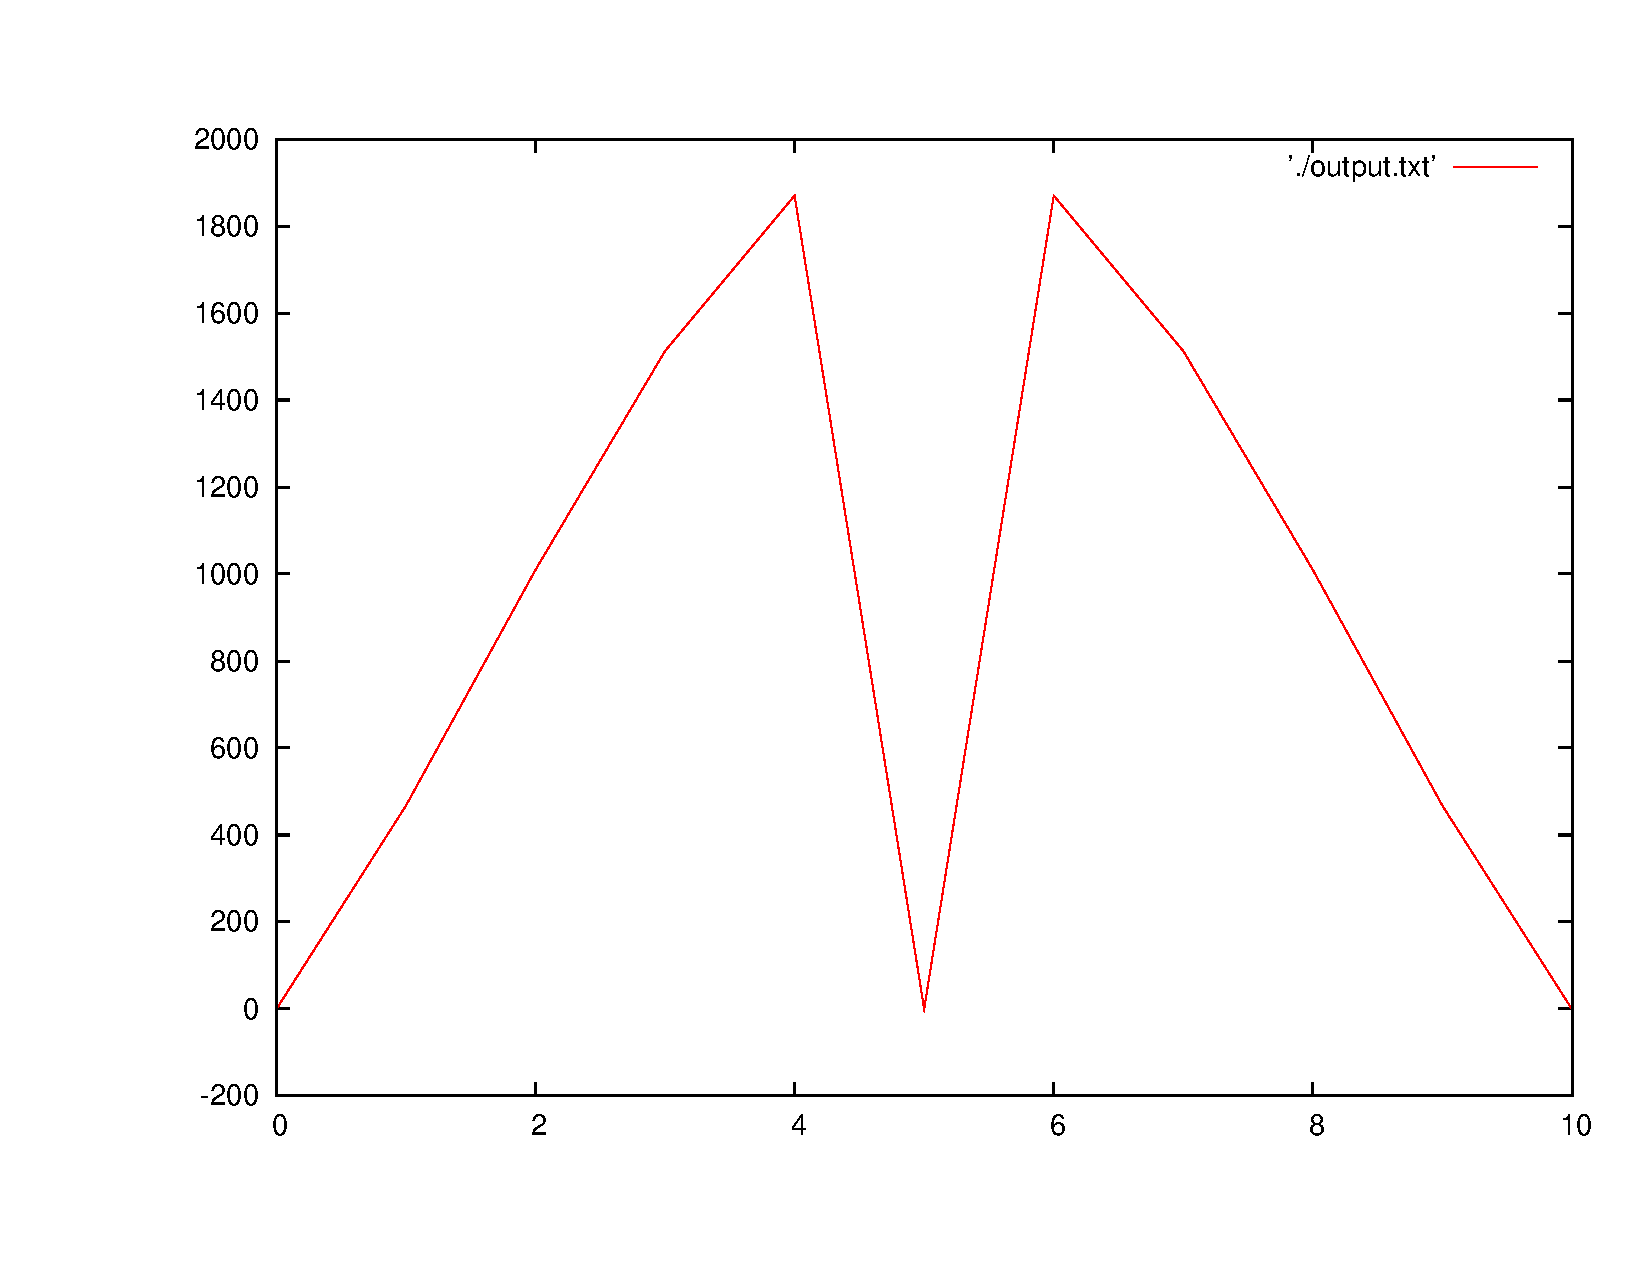
\includegraphics[width=.8\textwidth]{tms320c3x/fig_lp_output.pdf}
		\caption{\label{fig:tms320c3x_manual_lp_output} LP (Lowpass Finite Filter) output plot.}
	\end{center}
\end{figure}

This benchmark performs the computation of a LowPass Finite (LP) Filter over a digital signal.
The LP Filter is programmed in assembler using the \textit{z-transform}, which is widely utilized for the analysis of discrete-time signals, simular to the Laplace transform for continuous-time signals.
The implementation is based on the algorithm description provided in ``\textit{Digital Signal Processing: Laboratory Experiments Using C and the TMS320C31 DSK}'' book by Rulph Chassaing (1999, John Wiley \& Sons, Inc.).

The benchmark is mainly written in assembler, and it has been modified to accept an input signal within the ``\texttt{input\_signal.txt}'' file, to automatically compute the coefficients depending on the input signal length and to generate an output on the ``\texttt{output.txt}'' file.

This benchmark has been selected to globally check the sequential behavior of floating point instructions and the parallel floating point instructions.

This benchmark requires the TI C I/O service enabled to run in the TMS320C3X simulator.
A precompiled binary (\texttt{bp45.out}) is provided together with a GNU Make compatible Makefile.
A simulation configuration file (\texttt{sim\_config.xml}) for this benchmark is also provided, so that the simulator can run the benchmark with the following command:
  
\begin{verbatim}
$ unisim-tms320c3x-2.0 -c sim_config.xml
\end{verbatim}

The expected output data set is in the \texttt{output.ref.txt} file.
You can use plotting tools like \textit{gnuplot} to plot the generated output. 

Figure~\ref{fig:tms320c3x_manual_lp_output} shows the plot of \texttt{output.txt} using the following command under \textit{gnuplot}:

\begin{verbatim}
gnuplot > plot './output.txt' with lines
\end{verbatim}

\subsubsection{BP (Bandpass Finite Filter)}
\label{tms320c3x_sec:benchmarks_bp}

\begin{figure}[!h]
	\begin{center}
		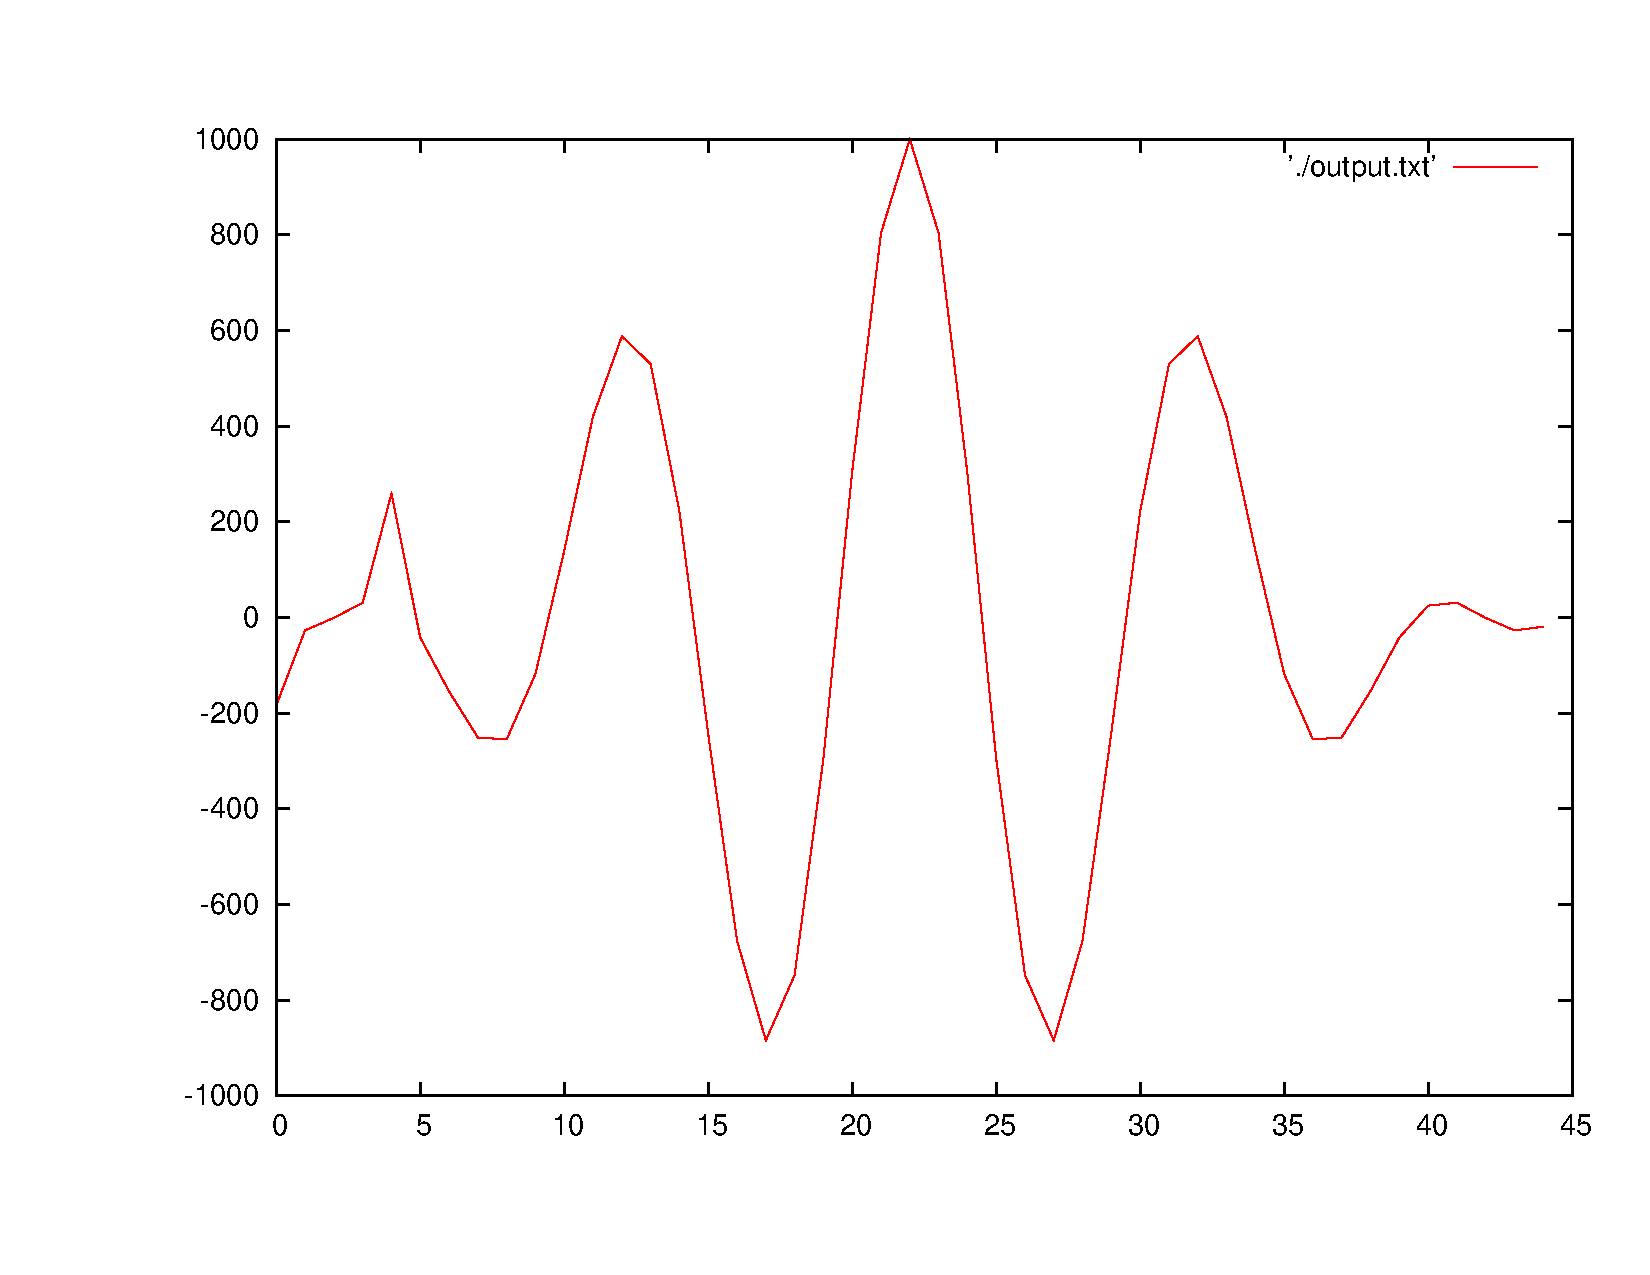
\includegraphics[width=.8\textwidth]{tms320c3x/fig_bp_output.pdf}
		\caption{\label{fig:tms320c3x_manual_bp_output} BP (Bandpass Finite Filter) output plot.}
	\end{center}
\end{figure}

This benchmark performs the computation of a BandPass Finite (LP) Filter over a digital signal.
The LP Filter is programmed in assembler using the \textit{z-transform}, which is widely utilized for the analysis of discrete-time signals, simular to the Laplace transform for continuous-time signals.
The implementation is based on the algorithm description provided in ``\textit{Digital Signal Processing: Laboratory Experiments Using C and the TMS320C31 DSK}'' book by Rulph Chassaing (1999, John Wiley \& Sons, Inc.).
The benchmark is mainly written in assembler, and it has been modified to accept an input signal (only 45 coefficients are considered) within the ``\texttt{input\_signal.txt}'' file, and to generate an output on the ``\texttt{output.txt}'' file.

As for the LowPass filter benchmark, this benchmark has been selected to globally check the sequential behavior of floating point instructions and some parallel floating point instructions.

This benchmark requires the TI C I/O service enabled to run in the TMS320C3X simulator.
A precompiled binary (\texttt{bp45.out}) is provided together with a GNU Make compatible Makefile.
A simulation configuration file (\texttt{sim\_config.xml}) for this benchmark is also provided, so that the simulator can run the benchmark with the following command:
  
\begin{verbatim}
$ unisim-tms320c3x-2.0 -c sim_config.xml
\end{verbatim}

The expected output data set is in the \texttt{output.ref.txt} file.
You can use plotting tools like \textit{gnuplot} to plot the generated output. 

Figure~\ref{fig:tms320c3x_manual_bp_output} shows the plot of \texttt{output.txt} using the following command under \textit{gnuplot}:

\begin{verbatim}
gnuplot > plot './output.txt' with lines
\end{verbatim}

\subsubsection{IIR (Biquad Infinite Filter)}

\begin{figure}[!h]
	\begin{center}
		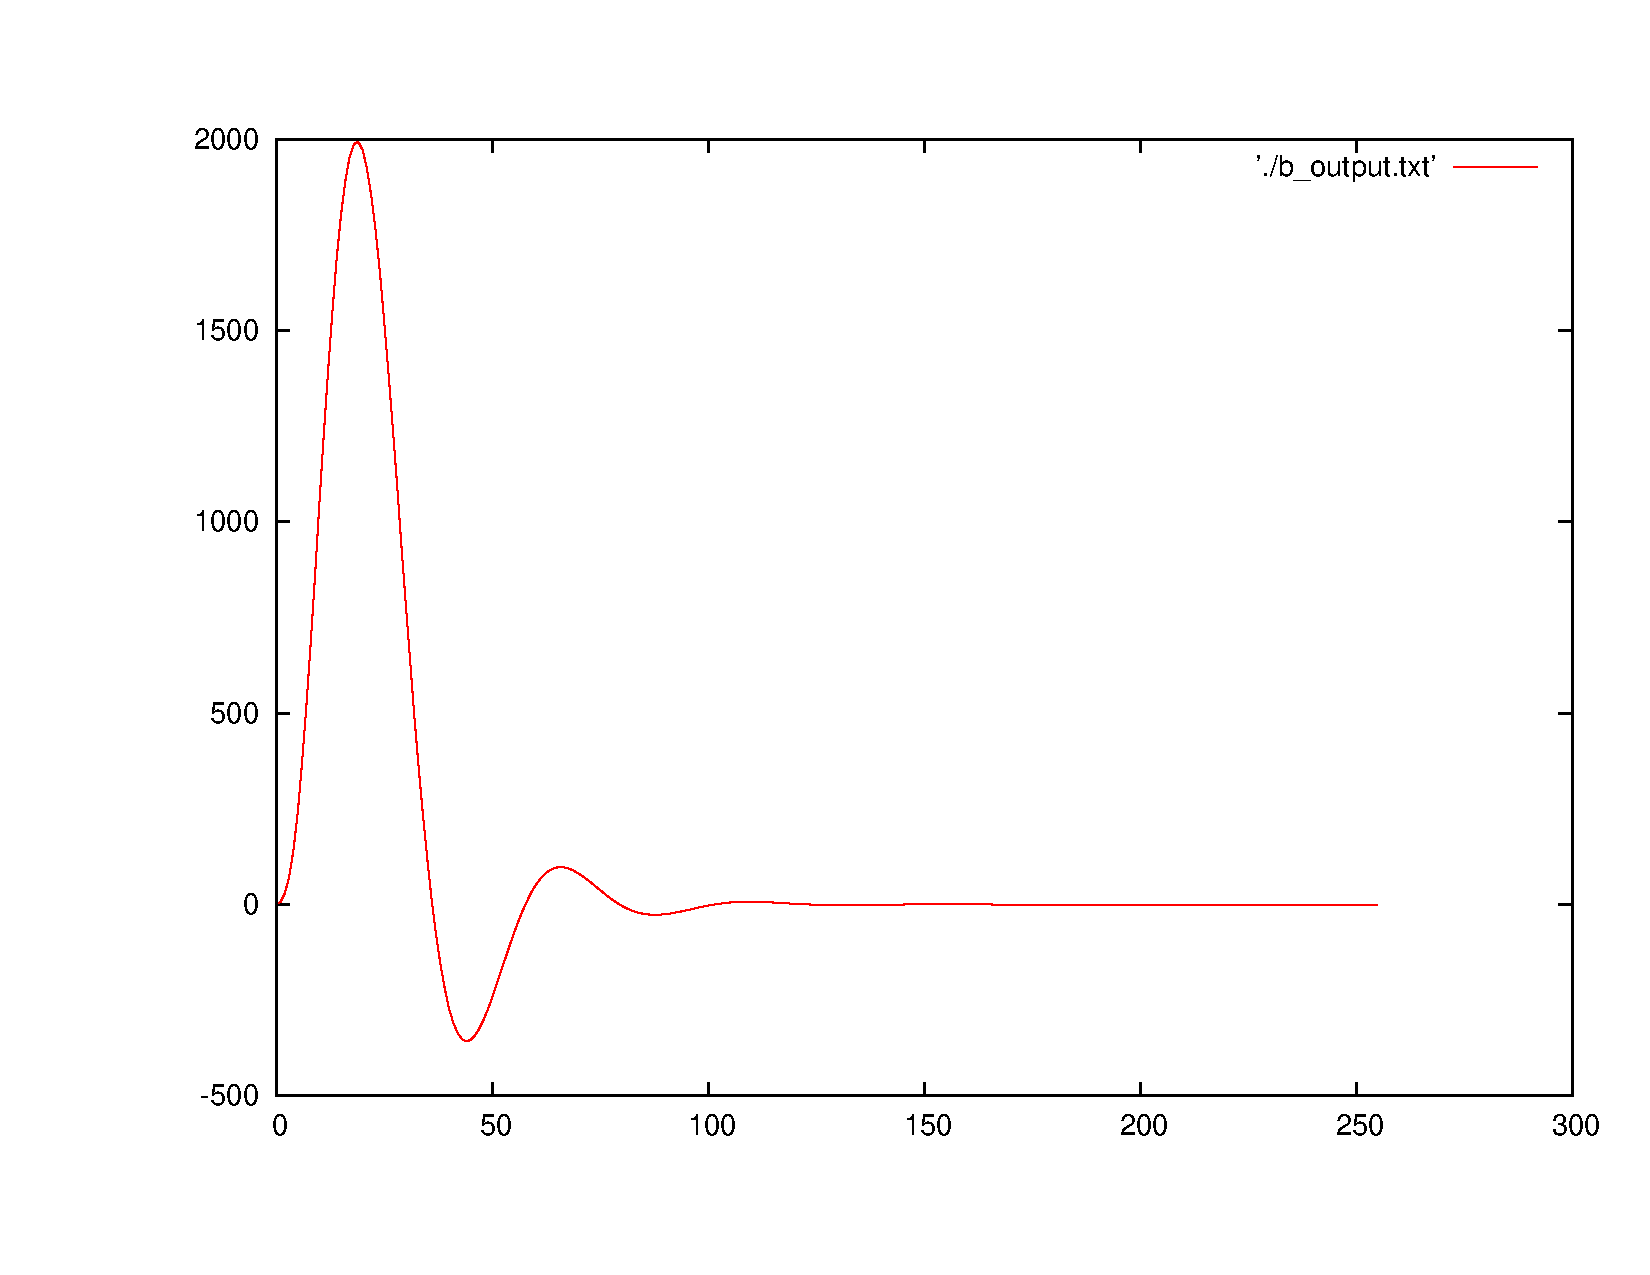
\includegraphics[width=.8\textwidth]{tms320c3x/fig_iir_output.pdf}
		\caption{\label{fig:tms320c3x_manual_iir_output}Plot of the IIR program using \textit{gnuplot}.}
	\end{center}
\end{figure}

This benchmarks performs the computation of an Infinite Impulse Response (IIR) Filter.
The previous filter benchmarks (see Sections~\ref{tms320c3x_sec:benchmarks_lp} and~\ref{tms320c3x_sec:benchmarks_bp}) do not have analog counterpart.
This filter benchmark makes use of the vast knowledge already acquired with analog filters.
The design procedure involves the conversion of an analog filter to an equivalent discrete filter using the bilinear transformation (BLT) technique.
As such, the BLT procedure converts a transfer function of an analog filter in the \textit{s}-domain into an equivalent discrete-time transfer function in the \textit{z}-domain.

This benchmark is based on two implementations of the biquad algorithm provided by the TI DSK 3 for the TMS320C3x.
The first implementation is done in pure C and uses floating point computation, and the second one is a fast version of the biquad algorithm programmed in assembler.
The benchmark provides at the end two different outputs, \texttt{b\_output.txt} for the C implementation and \texttt{fb\_output.txt} for the implementation in assembler.
Both outputs should be the same.

The IIR benchmark has been selected for the following reasons:
\begin{enumerate}
	\item It serves to check the correct sequential behavior of programs with an important use of floating point computations.
	\item It tests both floating point computations as generated by the TI C compiler and assembler code, which uses specialized instructions as parallel float computations.
	\item It tests complex addressing modes and specially the fast biquad implementation uses bit reverse addressing mode.
\end{enumerate}

This benchmark requires the TI C I/O service enabled to run in the TMS320C3X simulator.
A precompiled binary (\texttt{biquad4.out}) is provided together with a GNU Make compatible Makefile.
A simulation configuration file (\texttt{sim\_config.xml}) for this benchmark is also provided, so that the simulator can run the benchmark with the following command:
  
\begin{verbatim}
$ unisim-tms320c3x-2.0 -c sim_config.xml
\end{verbatim}

The expected output data set is in the \texttt{b\_output.ref.txt} and \texttt{fb\_output.ref.txt} files.
You can use plotting tools like \textit{gnuplot} to plot the generated outputs. 

Figure~\ref{fig:tms320c3x_manual_iir_output} shows the plot of \texttt{b\_output.txt} using the following command under \textit{gnuplot}:

\begin{verbatim}
gnuplot > plot './b_output.txt' with lines
\end{verbatim}

\subsubsection{FFT (Fast Fourier Transform)}

\begin{figure}[!h]
	\begin{center}
		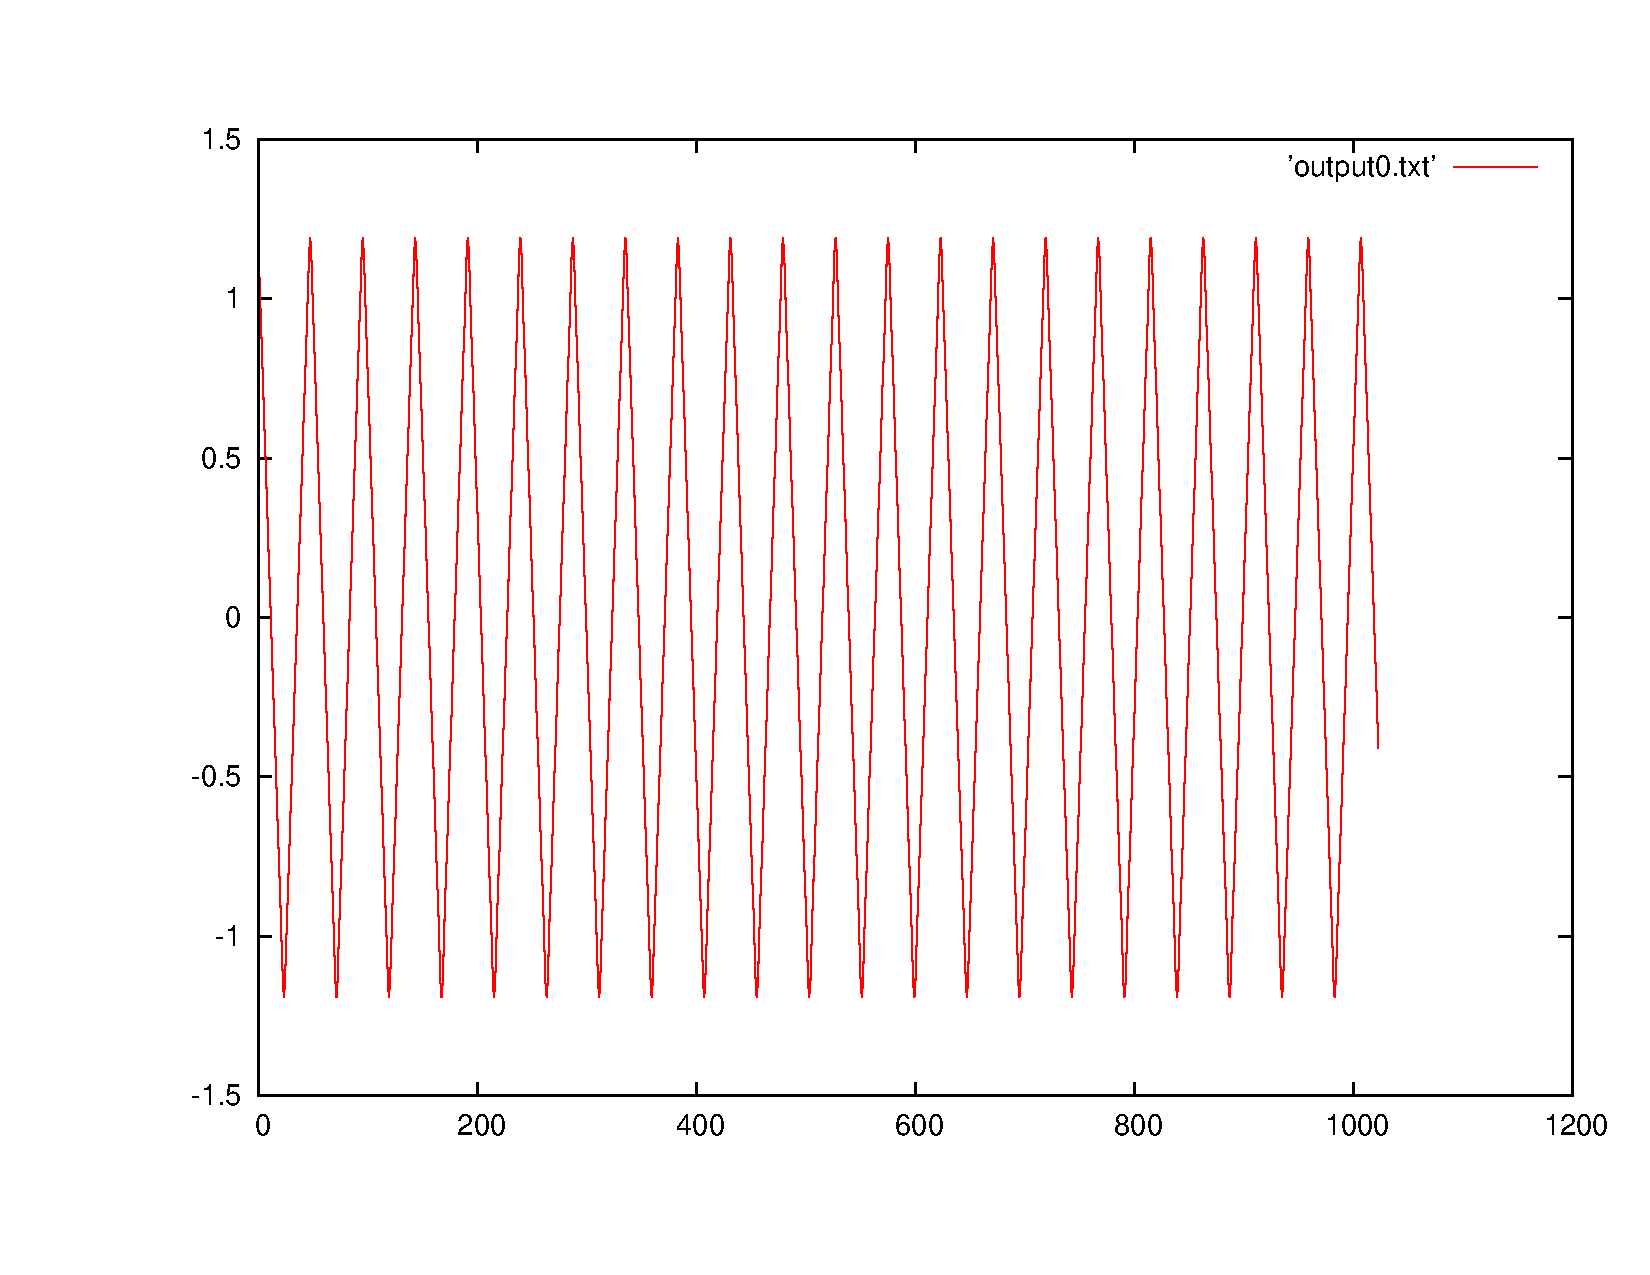
\includegraphics[width=.8\textwidth]{tms320c3x/fig_fft512_output0.pdf}
		\caption{\label{fig:tms320c3x_manual_fft_output0}Plot of the FFT512 program first iteration using \textit{gnuplot}.}
	\end{center}
\end{figure}

This benchmark simply computes a 512-point FFT (Fast Fourier Transform) using a Complex Radix 2 given a signal input.
It is based on the FFT codes provided by the TI DSK 3 for the TMS320C3x, modified to accept an input signal described as frequency and amplitude in two different input files: \textit{freq\_input.txt} (for the frequency) and \textit{ampl\_input.txt} (for the amplitude).
The benchmarks performs ten FFT iterations over the input signal and generates an output file for each of the iterations (\textit{output*.txt}, where ``*'' is the iteration number).

The FFT benchmark has been selected for the following reasons:
\begin{enumerate}
	\item As for the other floating point benchmarks it serves to check the correct sequential behavior of programs with an important use of floating point computations.
	\item Most of the program is written in assembler, using parallel float instructions that would otherwise have not been tested by the C compiler.
	\item The used FFT assembler implementation uses the bit reverse addressing mode, which is particularly well suited for FFT computations.
\end{enumerate} 

This benchmark requires the TI C I/O service enabled to run in the TMS320C3X simulator.
A precompiled binary (\texttt{fft.out}) is provided together with a GNU Make compatible Makefile.
A simulation configuration file (\texttt{sim\_config.xml}) for this benchmark is also provided, so that the simulator can run the benchmark with the following command:

\begin{verbatim}
$ unisim-tms320c3x-2.0 -c sim_config.xml
\end{verbatim}

The expected output data set is in the following files: \texttt{output0.ref.txt}, \texttt{output1.ref.txt}, \texttt{output2.ref.txt}, \texttt{output3.ref.txt}, \texttt{output4.ref.txt}, \texttt{output5.ref.txt}, \texttt{output6.ref.txt}, \texttt{output7.ref.txt}, \texttt{output8.ref.txt}, and \texttt{output9.ref.txt}.
You can use plotting tools like \textit{gnuplot} to plot the generated outputs. 

Figure~\ref{fig:tms320c3x_manual_fft_output0} shows the plot of \texttt{output0.txt} using the following command under \textit{gnuplot}:

\begin{verbatim}
gnuplot > plot './output0.txt' with lines
\end{verbatim}

\subsection{Instruction level unit tests}

As explained in Section~\ref{tms320c3x_benchmarks}, although they have validated general operations of the UNISIM TMS320C3X simulator, both the integer and floating-point benchmarks have insufficiently covered the TMS320C3X instructions.
Extensive testings at the instruction level are essential to gain greater confidence in the UNISIM TMS320C3X simulator representativity.
This section presents the validation process of UNISIM TMS320C3X simulator at the instruction level.
A unit testing environment, in the form of a Makefile for GNU Make, has been developed to allow testing individual instructions for the UNISIM TMS320C3X simulator.
Testing an instruction involves writing some "glue" code (C and Assembly) around the instruction under test to provide it with the input operands read from the host filesystem, and to save instruction output operands into a file on the host filesystem, so that results of instruction under test can be observed and compared.
A unit test generator, that is part of the testing environment, automatically generates that "glue" code, making writing and maintaining the instruction level unit tests easier.

Section~\ref{tms320c3x_validation_process} presents the validation process and the test plan.
Section~\ref{tms320c3x_testing_status} contains the testing status at instruction level of UNISIM TMS320C3X simulator.
Section~\ref{tms320c3x_unit_tests_generator} presents the unit tests generator flow.
Section~\ref{tms320c3x_testing_environment} presents the testing environment and Section~\ref{tms320c3x_regression_tests} shows how to use it as a regression test for the UNISIM TMS320C3X simulator.

\subsubsection{Validation process}
\label{tms320c3x_validation_process}

For the purpose of validating the UNISIM TMS320C3X simulator, a factorial plan has been established. 
The factorial plan parameters are:
\begin{itemize}
\item The general instruction under test, e.g. \texttt{ldf}, see Tables~\ref{table:tms320c3x_load_store_instructions}, \ref{table:tms320c3x_interlocked_instructions},  \ref{table:tms320c3x_control_instructions}, \ref{table:tms320c3x_2ops_instructions}, \ref{table:tms320c3x_3ops_instructions}, \ref{table:tms320c3x_parallel_instructions} and \ref{table:tms320c3x_power_instructions}
\item The condition code, e.g. \texttt{eq} in \texttt{ldfeq}, see Table~\ref{table:tms320c3x_condition_codes}
\item The general addressing mode (e.g. \texttt{indir} in \texttt{ldfeq indir, reg}), see Table~\ref{table:tms320c3x_general_addressing_modes}:
	\begin{itemize}
		\item For an immediate addressing mode, the immediate value
		\item For an indirect addressing mode, one of 26 available indirect addressing modes, see Table~\ref{table:tms320c3x_indir_addressing_modes}
	\end{itemize}
\item The input value set of the instruction, e.g. the value of \texttt{indir} memory operand in \texttt{ldfeq indir, reg}
\end{itemize}

\begin{table}[!p]
\begin{center}
	\small
	\begin{tabular}{|p{3.0cm}|p{10.0cm}|}
	\hline
	\textbf{Instructions} & \textbf{Description}\\
	\hline
	\textbf{lde} & Load Floating-Point Exponent\\
	\hline
	\textbf{ldf} & Load Floating-Point Value\\
	\hline
	\textbf{ldf\textit{cond}} & Load Floating-point Value Conditionally\\
	\hline
	\textbf{ldi} & Load Integer\\
	\hline
	\textbf{ldi\textit{cond}} & Load Integer Conditionally\\
	\hline
	\textbf{ldm} & Load Floating-Point Mantissa\\
	\hline
	\textbf{ldp} & Load Data-Page Pointer\\
	\hline
	\textbf{pop} & Pop Integer\\
	\hline
	\textbf{popf} & Pop Floating-Point Value\\
	\hline
	\textbf{push} & Push Integer\\
	\hline
	\textbf{pushf} & Push Floating-Point Value\\
	\hline
	\textbf{stf} & Store Floating-Point Value\\
	\hline
	\textbf{sti} & Store Integer\\
	\hline
	\end{tabular}
	\caption{\label{table:tms320c3x_load_store_instructions} TMS320C3X Load/Store Instructions.}
\end{center}
\end{table}

\begin{table}[!p]
\begin{center}
	\small
	\begin{tabular}{|p{3.0cm}|p{10.0cm}|}
	\hline
	\textbf{Instructions} & \textbf{Description}\\
	\hline
	\textbf{ldfi} & Load Floating-Point Value, Interlocked\\
	\hline
	\textbf{ldii} & Load Integer, Interlocked\\
	\hline
	\textbf{sigi} & Signal, Interlocked\\
	\hline
	\textbf{stfi} & Store Floating-Point Value, Interlocked\\
	\hline
	\textbf{stii} & Store Integer, Interlocked\\
	\hline
	\end{tabular}
	\caption{\label{table:tms320c3x_interlocked_instructions} TMS320C3X Interlocked Instructions.}
\end{center}
\end{table}

\begin{table}[!p]
\begin{center}
	\small
	\begin{tabular}{|p{3.0cm}|p{10.0cm}|}
	\hline
	\textbf{Instructions} & \textbf{Description}\\
	\hline
	\textbf{b\textit{cond}} & Branch Conditionally (Standard)\\
	\hline
	\textbf{b\textit{cond}d} & Branch Conditionally (Delayed)\\
	\hline
	\textbf{br} & Branch Unconditionally (Standard)\\
	\hline
	\textbf{brd} & Branch Unconditionally (Delayed)\\
	\hline
	\textbf{call} & Call Subroutine\\
	\hline
	\textbf{call\textit{cond}} & Call Subroutine Conditionally\\
	\hline
	\textbf{db\textit{cond}} & Decrement and Branch Conditionally (Standard)\\
	\hline
	\textbf{db\textit{cond}d} & Decrement and Branch Conditionally (Delayed)\\
	\hline
	\textbf{iack} & Interrupt Acknowledge\\
	\hline
	\textbf{idle} & Idle Until Interrupt\\
	\hline
	\textbf{nop} & No Operation\\
	\hline
	\textbf{reti\textit{cond}} & Return From Interrupt Conditionally\\
	\hline
	\textbf{rets\textit{cond}} & Return From Subroutine Conditionally\\
	\hline
	\textbf{rptb} & Repeat Block\\
	\hline
	\textbf{rpts} & Repeat Single Instruction\\
	\hline
	\textbf{swi} & Software Interrupt\\
	\hline
	\textbf{trap\textit{cond}} & Trap Conditionally\\
	\hline
	\end{tabular}
	\caption{\label{table:tms320c3x_control_instructions} TMS320C3X Control Instructions.}
\end{center}
\end{table}

\begin{table}[!p]
\begin{center}
	\small
	\begin{tabular}{|p{3.0cm}|p{10.0cm}|}
	\hline
	\textbf{Instructions} & \textbf{Description}\\
	\hline
	\textbf{absf} & Absolute Value of Floating-Point\\
	\hline
	\textbf{absi} & Absolute Value of Integer\\
	\hline
	\textbf{addc} & Add Integer With Carry\\
	\hline
	\textbf{addf} & Add Floating-Point Values\\
	\hline
	\textbf{addi} & Add Integer\\
	\hline
	\textbf{and} & Bitwise-Logical AND\\
	\hline
	\textbf{andn} & Bitwise-Logical AND With Complement\\
	\hline
	\textbf{ash} & Arithmetic Shift\\
	\hline
	\textbf{cmpf} & Compare Floating-Point Value\\
	\hline
	\textbf{cmpi} & Compare Integer\\
	\hline
	\textbf{fix} & Floating-Point-to-Integer Conversion\\
	\hline
	\textbf{float} & Integer-to-Floating-Point Conversion\\
	\hline
	\textbf{lsh} & Logical Shift\\
	\hline
	\textbf{mpyf} & Multiply Floating-Point Value\\
	\hline
	\textbf{mpyi} & Multiply Integer\\
	\hline
	\textbf{negb} & Negative Integer With Borrow\\
	\hline
	\textbf{negf} & Negative Floating-Point Value\\
	\hline
	\textbf{negi} & Negate Integer\\
	\hline
	\textbf{norm} & Normalize\\
	\hline
	\textbf{not} & Bitwise-Logical Complement\\
	\hline
	\textbf{or} & Bitwise-Logical OR\\
	\hline
	\textbf{rnd} & Round Floating-Point Value\\
	\hline
	\textbf{rol} & Rotate Left\\
	\hline
	\textbf{rolc} & Rotate Left Through Carry\\
	\hline
	\textbf{ror} & Rotate Right\\
	\hline
	\textbf{rorc} & Rotate Right Through Carry\\
	\hline
	\textbf{subb} & Substract Integer With Borrow\\
	\hline
	\textbf{subc} & Substract Integer Conditionally\\
	\hline
	\textbf{subf} & Substract Floating-Point Value\\
	\hline
	\textbf{subi} & Substract Integer\\
	\hline
	\textbf{subrb} & Substract Reverse Integer With Borrow\\
	\hline
	\textbf{subrf} & Substract Reverse Floating-Point Value\\
	\hline
	\textbf{subri} & Substract Reverse Integer\\
	\hline
	\textbf{tstb} & Test Bit Fields\\
	\hline
	\textbf{xor} & Bitwise-Exclusive OR\\
	\hline
	\end{tabular}
	\caption{\label{table:tms320c3x_2ops_instructions} TMS320C3X 2-operand Instructions.}
\end{center}
\end{table}

\begin{table}[!p]
\begin{center}
	\small
	\begin{tabular}{|p{3.0cm}|p{10.0cm}|}
	\hline
	\textbf{Instructions} & \textbf{Description}\\
	\hline
	\textbf{addc3} & Add Integer With Carry, 3-Operand\\
	\hline
	\textbf{addf3} & Add Floating-Point, 3-Operand\\
	\hline
	\textbf{addi3} & Add Integer, 3-Operand\\
	\hline
	\textbf{and3} & Bitwise-Logical AND, 3-Operand\\
	\hline
	\textbf{andn3} & Bitwise-Logical AND With Complement, 3-Operand\\
	\hline
	\textbf{ash3} & Arithmetic Shift, 3-Operand\\
	\hline
	\textbf{cmpf3} & Compare Floating-Point Value, 3-Operand\\
	\hline
	\textbf{cmpi3} & Compare Integer, 3-Operand\\
	\hline
	\textbf{lsh3} & Logical Shift, 3-Operand\\
	\hline
	\textbf{mpyf3} & Multiply Floating-Point Value, 3-Operand\\
	\hline
	\textbf{mpyi3} & Multiply Integer, 3-Operand\\
	\hline
	\textbf{or3} & Bitwise-Logical OR, 3-Operand\\
	\hline
	\textbf{subb3} & Substract Integer With Borrow, 3-Operand\\
	\hline
	\textbf{subf3} & Substract Floating-Point Value, 3-Operand\\
	\hline
	\textbf{subi3} & Substract Integer, 3-Operand\\
	\hline
	\textbf{tstb3} & Test Bit Fields, 3-Operand\\
	\hline
	\textbf{xor3} & Bitwise-Exclusive OR, 3-Operand\\
	\hline
	\end{tabular}
	\caption{\label{table:tms320c3x_3ops_instructions} TMS320C3X 3-operand Instructions.}
\end{center}
\end{table}

\begin{table}[!p]
\begin{center}
	\small
	\begin{tabular}{|p{3.0cm}|p{10.0cm}|}
	\hline
	\textbf{Instructions} & \textbf{Description}\\
	\hline
	\textbf{absf}\texttt{~||~}\textbf{stf} & Parallel absf and stf\\
	\hline
	\textbf{absi}\texttt{~||~}\textbf{sti} & Parallel absi and sti\\
	\hline
	\textbf{addf3}\texttt{~||~}\textbf{stf} & Parallel addf3 and stf\\
	\hline
	\textbf{addi3}\texttt{~||~}\textbf{sti} & Parallel addi3 and sti\\
	\hline
	\textbf{and3}\texttt{~||~}\textbf{sti} & Parallel and3 and sti\\
	\hline
	\textbf{ash3}\texttt{~||~}\textbf{sti} & Parallel ash3 and sti\\
	\hline
	\textbf{fix}\texttt{~||~}\textbf{sti} & Parallel fix and sti\\
	\hline
	\textbf{float}\texttt{~||~}\textbf{sti} & Parallel float and stf\\
	\hline
	\textbf{ldf}\texttt{~||~}\textbf{ldf} & Parallel ldf and ldf\\
	\hline
	\textbf{ldf}\texttt{~||~}\textbf{stf} & Parallel ldf and stf\\
	\hline
	\textbf{ldi}\texttt{~||~}\textbf{ldi} & Parallel ldi and ldi\\
	\hline
	\textbf{ldi}\texttt{~||~}\textbf{sti} & Parallel ldi and sti\\
	\hline
	\textbf{lsh3}\texttt{~||~}\textbf{sti} & Parallel lsh3 and sti\\
	\hline
	\textbf{mpyf3}\texttt{~||~}\textbf{addf3} & Parallel mpyf3 and addf3\\
	\hline
	\textbf{mpyf3}\texttt{~||~}\textbf{stf} & Parallel mpyf3 and stf\\
	\hline
	\textbf{mpyf3}\texttt{~||~}\textbf{subf3} & Parallel mpyf3 and subf3\\
	\hline
	\textbf{mpyi3}\texttt{~||~}\textbf{addi3} & Parallel mpyi3 and addi3\\
	\hline
	\textbf{mpyi3}\texttt{~||~}\textbf{sti} & Parallel mpyi3 and sti\\
	\hline
	\textbf{mpyi3}\texttt{~||~}\textbf{subi3} & Parallel mpyi3 and subi3\\
	\hline
	\textbf{negf}\texttt{~||~}\textbf{stf} & Parallel negf and stf\\
	\hline
	\textbf{negi}\texttt{~||~}\textbf{sti} & Parallel negi and sti\\
	\hline
	\textbf{not}\texttt{~||~}\textbf{sti} & Parallel not and sti\\
	\hline
	\textbf{or3}\texttt{~||~}\textbf{sti} & Parallel or3 and sti\\
	\hline
	\textbf{stf}\texttt{~||~}\textbf{stf} & Parallel Store Floating-Point Value\\
	\hline
	\textbf{sti}\texttt{~||~}\textbf{sti} & Parallel sti and sti\\
	\hline
	\textbf{subf3}\texttt{~||~}\textbf{stf} & Parallel subf3 and stf\\
	\hline
	\textbf{subi3}\texttt{~||~}\textbf{sti} & Parallel subi3 and sti\\
	\hline
	\textbf{xor3}\texttt{~||~}\textbf{sti} & Parallel xor3 and sti\\
	\hline
	\end{tabular}
	\caption{\label{table:tms320c3x_parallel_instructions} TMS320C3X Parallel Instructions.}
\end{center}
\end{table}

\begin{table}[!p]
\begin{center}
	\small
	\begin{tabular}{|p{3.0cm}|p{10.0cm}|}
	\hline
	\textbf{Instructions} & \textbf{Description}\\
	\hline
	\textbf{idle2} & Low-Power Idle\\
	\hline
	\textbf{lopower} & Divide Clock by 16\\
	\hline
	\textbf{maxspeed} & Restore Clock to Regular Speed\\
	\hline
	\end{tabular}
	\caption{\label{table:tms320c3x_power_instructions} TMS320C3X Parallel Instructions.}
\end{center}
\end{table}

\begin{table}[!p]
\begin{center}
	\small
	\begin{tabular}{|p{3.0cm}|p{10.0cm}|}
	\hline
	\textbf{Condition codes (20)} & \textbf{Description}\\
	\hline
	\texttt{u} & unconditional \\
	\hline
	\texttt{lo} & lower than\\
	\hline
	\texttt{ls} & lower than or same as\\
	\hline
	\texttt{hi} & higher than\\
	\hline
	\texttt{hs} & higher than or same as\\
	\hline
	\texttt{eq} & equal\\
	\hline
	\texttt{ne} & not equal\\
	\hline
	\texttt{lt} & less than\\
	\hline
	\texttt{le} & less than or equal\\
	\hline
	\texttt{gt} & greater than\\
	\hline
	\texttt{ge} & greater than or equal\\
	\hline
	\texttt{nv} & no overflow\\
	\hline
	\texttt{v} & overflow\\
	\hline
	\texttt{nuf} & no floating-point underflow\\
	\hline
	\texttt{uf} & floating-point underflow\\
	\hline
	\texttt{nlv} & no overflow\\
	\hline
	\texttt{lv} & overflow\\
	\hline
	\texttt{nluf} & no latched floating-point underflow\\
	\hline
	\texttt{luf} & latched floating-point underflow\\
	\hline
	\texttt{zuf} & zero or floating-point underflow\\
	\hline
	\end{tabular}
	\caption{\label{table:tms320c3x_condition_codes} Condition codes.}
\end{center}
\end{table}

\begin{table}[!p]
\begin{center}
	\small
	\begin{tabular}{|p{3.0cm}|p{12.0cm}|}
	\hline
	\textbf{General\newline Addressing \newline Modes (4)} & \textbf{Description}\\
	\hline
	reg & register addressing mode\\
	\hline
	dir & direct addressing mode\\
	\hline
	imm & immediate addressing mode\\
	\hline
	indir & indirect addressing mode (see table)\\
	\hline
	\end{tabular}
	\caption{\label{table:tms320c3x_general_addressing_modes} General addressing modes.}
\end{center}
\end{table}

\begin{table}[!p]
\begin{center}
	\small
	\begin{tabular}{|p{2.3cm}|p{2.3cm}|p{11.0cm}|}
	\hline
	\textbf{Indirect\newline Addressing \newline Modes (26)} & \textbf{Tests} & \textbf{Description}\\
	\hline
	\texttt{*+ar$_n$(disp)} & \texttt{*+ar$_n$(1)} & indirect addressing with predisplacement add\\
	\hline
	\texttt{*-ar$_n$(disp)} & \texttt{*-ar$_n$(1)} & indirect addressing with predisplacement subtract\\
	\hline
	\texttt{*++ar$_n$(disp)} & \texttt{*++ar$_n$(1)} & indirect addressing with predisplacement add and modify\\
	\hline
	\texttt{*--ar$_n$(disp)} & \texttt{*--ar$_n$(1)} & indirect addressing with predisplacement substract and modify\\
	\hline
	\texttt{*ar$_n$++(disp)} & \texttt{*ar$_n$++(1)} & indirect addressing with postdisplacement add and modify\\
	\hline
	\texttt{*ar$_n$--(disp)} & \texttt{*ar$_n$--(1)} & indirect addressing with postdisplacement substract and modify\\
	\hline
	\texttt{*ar$_n$++(disp)\%} & \texttt{*ar$_n$++(1)\%} \newline \texttt{bk} $\in$ \{4,5\} & indirect addressing with postdisplacement add and circular modify\\
	\hline
	\texttt{*ar$_n$(disp)\%} & \texttt{*ar$_n$(disp)\%} \newline \texttt{bk} $\in$ \{4,5\} & indirect addressing with postdisplacement substract and circular modify\\
	\hline
	\texttt{*+ar$_n$(ir0)} & \texttt{*+ar$_n$(ir0)} \newline \texttt{ir0} $\in$ [0,15] & indirect addressing with preindex (ir0) add\\
	\hline
	\texttt{*-ar$_n$(ir0)} & \texttt{*-ar$_n$(ir0)} \newline \texttt{ir0} $\in$ [0,15] & indirect addressing with preindex (ir0) substract\\
	\hline
	\texttt{*++ar$_n$(ir0)} & \texttt{*++ar$_n$(ir0)} \newline \texttt{ir0} $\in$ [0,15] & indirect addressing with preindex (ir0) add and modify\\
	\hline
	\texttt{*--ar$_n$(ir0)} & \texttt{*--ar$_n$(ir0)} \newline \texttt{ir0} $\in$ [0,15] & indirect addressing with preindex (ir0) substract and modify\\
	\hline
	\texttt{*ar$_n$++(ir0)} & \texttt{*ar$_n$++(ir0)} \newline \texttt{ir0} $\in$ [0,15] & indirect addressing with postindex (ir0) add and modify\\
	\hline
	\texttt{*ar$_n$--(ir0)} & \texttt{*ar$_n$--(ir0)} \newline \texttt{ir0} $\in$ [0,15] & indirect addressing with postindex (ir0) substract and modify\\
	\hline
	\texttt{*ar$_n$++(ir0)\%} & \texttt{*ar$_n$++(ir0)\%} \newline \texttt{ir0} $\in$ [0,15] \newline \texttt{bk} $\in$ \{4,5\} & indirect addressing with postindex (ir0) add and circular modify\\
	\hline
	\texttt{*ar$_n$--(ir0)\%} & \texttt{*ar$_n$--(ir0)\%} \newline \texttt{ir0} $\in$ [0,15] \newline \texttt{bk} $\in$ \{4,5\} & indirect addressing with postindex (ir0) substract and circular modify\\
	\hline
	\texttt{*+ar$_n$(ir1)} & \texttt{*+ar$_n$(ir1)} \newline \texttt{ir1} $\in$ [0,15] & indirect addressing with preindex (ir1) add\\
	\hline
	\texttt{*-ar$_n$(ir1)} & \texttt{*-ar$_n$(ir1)} \newline \texttt{ir1} $\in$ [0,15] & indirect addressing with preindex (ir1) substract\\
	\hline
	\texttt{*++ar$_n$(ir1)} & \texttt{*++ar$_n$(ir1)} \newline \texttt{ir1} $\in$ [0,15] & indirect addressing with preindex (ir1) add and modify\\
	\hline
	\texttt{*--ar$_n$(ir1)} & \texttt{*--ar$_n$(ir1)} \newline \texttt{ir1} $\in$ [0,15] & indirect addressing with preindex (ir1) substract and modify\\
	\hline
	\texttt{*ar$_n$++(ir1)} & \texttt{*ar$_n$++(ir1)} \newline \texttt{ir1} $\in$ [0,15] & indirect addressing with postindex (ir1) add and modify\\
	\hline
	\texttt{*ar$_n$--(ir1)} & \texttt{*ar$_n$--(ir1)} \newline \texttt{ir1} $\in$ [0,15] & indirect addressing with postindex (ir1) substract and modify\\
	\hline
	\texttt{*ar$_n$++(ir1)\%} & \texttt{*ar$_n$++(ir1)\%} \newline \texttt{ir1} $\in$ [0,15] \newline \texttt{bk} $\in$ \{4,5\} & indirect addressing with postindex (ir1) add and circular modify\\
	\hline
	\texttt{*ar$_n$--(ir1)\%} & \texttt{*ar$_n$--(ir1)\%} \newline \texttt{ir1} $\in$ [0,15] \newline \texttt{bk} $\in$ \{4,5\} & indirect addressing with postindex (ir1) substract and circular modify\\
	\hline
	\texttt{*ar$_n$} & \texttt{*ar$_n$} & indirect addressing\\
	\hline
	\texttt{*ar$_n$++(ir0)b} & \texttt{*ar$_n$++(ir0)b} \newline \texttt{ir1} $\in$ [0,15] & indirect addressing with postindex (ir0) add and bit-reversed modify\\
	\hline
	\end{tabular}
	\caption{\label{table:tms320c3x_indir_addressing_modes} Indirect addressing modes.}
\end{center}
\end{table}

\FloatBarrier

This plan results in lot of instruction alternatives being tested (several condition codes and addressing modes).
A full exploration of the factorial plan would have resulted in an unreasonable number of unit tests.
To limit the number of unit tests and to still achieve a good testing status, the following choices have been done:
\begin{itemize}
\item The amount of immediate addressing have been limited because each unit test of immediate addressing results in one program. The following integer values have been tested: \texttt{0}, \texttt{-1}, \texttt{+1}, \texttt{-32768}, or \texttt{+32767}. These integer values have a special role in most integer computations (neutral element, bound of integer immediate value \ldots). The following floating-point values have been tested: \texttt{0.0}, \texttt{1.0}, \texttt{-1.0}, \texttt{1.5}, \texttt{-1.5}, \texttt{$2.5594 \cdot 10^2$}, \texttt{$7.8125 \cdot 10^{-3}$}, \texttt{$-7.8163 \cdot 10^{-3}$}, \texttt{$-2.56 \cdot 10^2$}. These floating-point value have a special role in most floating-point computations (neutral element, smallest/largest positive/negative immediate floating-point values \ldots).
\item Condition codes have been varied exhaustively for conditional load/store and control instructions, see Table~\ref{table:tms320c3x_condition_codes}.
\item Each general addressing mode has been tested for load/store, control, 2-operand, 3-operand, and parallel instructions (note: some instructions allow only few of them), see Table~\ref{table:tms320c3x_general_addressing_modes}.
\item All of the 26 indirect addressing modes have been tested for load/store instructions and 2-operand instructions (28 tests per instructions), see Table~\ref{table:tms320c3x_indir_addressing_modes}.
\item Only one (\texttt{*ar$_n$}) of the 26 indirect addressing modes have been tested for 3-operand instructions and parallel instructions because testing all combinations of the 26 indirect addressing modes would have resulted in an unreasonable number of unit tests.
The rational behind this choice is that the instructions implementations in the UNISIM TMS320C3X simulator share the same source code for the indirect addressing modes.
\item 2-operand instructions with register addressing have been tested 10000 times with random inputs.
\item 3-operand instructions, load/store instructions, and parallel instructions with register, direct and indirect addressing modes have been tested 100 times with random inputs.
\item Additional tests have been written to check \texttt{ar$_n$} update ordering when instruction has several operands with indirect addressing mode, or when \texttt{ar$_n$} is both updated by an indirect addressing mode and the instruction itself.
\item Random input integer values have an uniform distribution. Table~\ref{table:tms320c3x_unit_test_float_distribution} shows the distribution for the floating point numbers. Some remarkable values (neutral, smallest/largest positive/negative floating-point values \ldots) have non-null probability of occurrence.
\end{itemize}

These choices still have resulted in 3757 unit test programs for a total of 694282 unit tests.

\subsubsection{Testing status}
\label{tms320c3x_testing_status}

\noindent The table below summarizes the testing status of all instructions. 
The total number of unit tests is shown and the detail for the computation of that number is explained between parenthesis.
$100_{rand}$ means 100 tests with random inputs.
$5_{imm}$ means 5 tests with immediate addressing. 
$20_{cond}$ means 20 tests for each condition codes. 
$28_{indir}$ means 28 tests for each 26 indirect addressing mode. 
$1_{indir}$ means only \texttt{ar$_n$} indirect addressing mode tested. 
$28_{isr}$ means 28 interrupt service routines tested. 
$1_{ar}$ means one test for \texttt{ar$_n$} update ordering.

\newpage

\begin{center}
\tablehead{\hline
\multicolumn{1}{|c|}{\textbf{Instruction}} & \multicolumn{1}{|c|}{\textbf{Tested?}} & \multicolumn{1}{|c|}{\textbf{Description}}\\
\hline}
\tabletail{\hline}
\begin{supertabular}{|p{7.0cm}|p{1.0cm}|p{7.0cm}|}
\multicolumn{3}{|c|}{\textbf{lde}}\\
\hline
\multicolumn{1}{|p{7.0 cm}|}{\scriptsize \texttt{lde reg, reg}} & \multicolumn{1}{p{1.0cm}|}{Yes} & \multicolumn{1}{p{7.0cm}|}{100 unit tests ($100_{rand}$)}\\
\hline
\multicolumn{1}{|p{7.0cm}|}{\scriptsize \texttt{lde dir, reg}} & \multicolumn{1}{p{1.0cm}|}{Yes} & \multicolumn{1}{p{7.0cm}|}{100 unit tests ($100_{rand}$)}\\
\hline
\multicolumn{1}{|p{7.0cm}|}{\scriptsize \texttt{lde indir, reg}} & \multicolumn{1}{p{1.0cm}|}{Yes} & \multicolumn{1}{p{7.0cm}|}{2800 unit tests ($28_{indir} \times 100_{rand}$)}\\
\hline
\multicolumn{1}{|p{7.0cm}|}{\scriptsize \texttt{lde imm, reg}} & \multicolumn{1}{p{1.0cm}|}{Yes} & \multicolumn{1}{p{7.0cm}|}{5 unit tests ($5_{imm}$)}\\
\hline
\multicolumn{3}{|c|}{\textbf{ldf}}\\
\hline
\multicolumn{1}{|p{7.0cm}|}{\scriptsize \texttt{ldf reg, reg}} & \multicolumn{1}{p{1.0cm}|}{Yes} & \multicolumn{1}{p{7.0cm}|}{100 unit tests ($100_{rand}$)}\\
\hline
\multicolumn{1}{|p{7.0cm}|}{\scriptsize \texttt{ldf dir, reg}} & \multicolumn{1}{p{1.0cm}|}{Yes} & \multicolumn{1}{p{7.0cm}|}{100 unit tests ($100_{rand}$)}\\
\hline
\multicolumn{1}{|p{7.0cm}|}{\scriptsize \texttt{ldf indir, reg}} & \multicolumn{1}{p{1.0cm}|}{Yes} & \multicolumn{1}{p{7.0cm}|}{2800 unit tests ($28_{indir} \times 100_{rand}$)}\\
\hline
\multicolumn{1}{|p{7.0cm}|}{\scriptsize \texttt{ldf imm, reg}} & \multicolumn{1}{p{1.0cm}|}{Yes} & \multicolumn{1}{p{7.0cm}|}{5 unit tests ($5_{imm}$)}\\
\hline
\multicolumn{3}{|c|}{\textbf{ldf\textit{cond}}}\\
\hline
\multicolumn{1}{|p{7.0cm}|}{\scriptsize \texttt{ldf\textit{cond} reg, reg}} & \multicolumn{1}{p{1.0cm}|}{Yes} & \multicolumn{1}{p{7.0cm}|}{2000 unit tests ($20_{cond} \times 100_{rand}$)}\\
\hline
\multicolumn{1}{|p{7.0cm}|}{\scriptsize \texttt{ldf\textit{cond} dir, reg}} & \multicolumn{1}{p{1.0cm}|}{Yes} & \multicolumn{1}{p{7.0cm}|}{2000 unit tests ($20_{cond} \times 100_{rand}$)}\\
\hline
\multicolumn{1}{|p{7.0cm}|}{\scriptsize \texttt{ldf\textit{cond} indir, reg}} & \multicolumn{1}{p{1.0cm}|}{Yes} & \multicolumn{1}{p{7.0cm}|}{56K unit tests ($28_{indir} \times 20_{cond} \times 100_{rand}$)}\\
\hline
\multicolumn{1}{|p{7.0cm}|}{\scriptsize \texttt{ldf\textit{cond} imm, reg}} & \multicolumn{1}{p{1.0cm}|}{Yes} & \multicolumn{1}{p{7.0cm}|}{100 unit tests ($100_{rand}$)}\\
\hline
\multicolumn{3}{|c|}{\textbf{ldi}}\\
\hline
\multicolumn{1}{|p{7.0cm}|}{\scriptsize \texttt{ldi reg, reg}} & \multicolumn{1}{p{1.0cm}|}{Yes} & \multicolumn{1}{p{7.0cm}|}{100 unit tests ($100_{rand}$)}\\
\hline
\multicolumn{1}{|p{7.0cm}|}{\scriptsize \texttt{ldi dir, reg}} & \multicolumn{1}{p{1.0cm}|}{Yes} & \multicolumn{1}{p{7.0cm}|}{100 unit tests ($100_{rand}$)}\\
\hline
\multicolumn{1}{|p{7.0cm}|}{\scriptsize \texttt{ldi indir, reg}} & \multicolumn{1}{p{1.0cm}|}{Yes} & \multicolumn{1}{p{7.0cm}|}{2900 unit tests ($(28_{indir} + 1_{ar}) \times 100_{rand}$)}\\
\hline
\multicolumn{1}{|p{7.0cm}|}{\scriptsize \texttt{ldi imm, reg}} & \multicolumn{1}{p{1.0cm}|}{Yes} & \multicolumn{1}{p{7.0cm}|}{5 unit tests ($5_{imm}$)}\\
\hline
\multicolumn{3}{|c|}{\textbf{ldi\textit{cond}}}\\
\hline
\multicolumn{1}{|p{7.0cm}|}{\scriptsize \texttt{ldi\textit{cond} reg, reg}} & \multicolumn{1}{p{1.0cm}|}{Yes} & \multicolumn{1}{p{7.0cm}|}{2000 unit tests ($20_{cond} \times 100_{rand}$)}\\
\hline
\multicolumn{1}{|p{7.0cm}|}{\scriptsize \texttt{ldi\textit{cond} dir, reg}} & \multicolumn{1}{p{1.0cm}|}{Yes} & \multicolumn{1}{p{7.0cm}|}{2000 unit tests ($20_{cond} \times 100_{rand}$)}\\
\hline
\multicolumn{1}{|p{7.0cm}|}{\scriptsize \texttt{ldi\textit{cond} indir, reg}} & \multicolumn{1}{p{1.0cm}|}{Yes} & \multicolumn{1}{p{7.0cm}|}{56K unit tests ($(28_{indir} + 1_{ar}) \times 20_{cond} \times 100_{rand}$)}\\
\hline
\multicolumn{1}{|p{7.0cm}|}{\scriptsize \texttt{ldi\textit{cond} imm, reg}} & \multicolumn{1}{p{1.0cm}|}{Yes} & \multicolumn{1}{p{7.0cm}|}{100 unit tests ($100_{rand}$)}\\
\hline
\multicolumn{3}{|c|}{\textbf{ldm}}\\
\hline
\multicolumn{1}{|p{7.0cm}|}{\scriptsize \texttt{ldm reg, reg}} & \multicolumn{1}{p{1.0cm}|}{Yes} & \multicolumn{1}{p{7.0cm}|}{100 unit tests ($100_{rand}$)}\\
\hline
\multicolumn{1}{|p{7.0cm}|}{\scriptsize \texttt{ldm dir, reg}} & \multicolumn{1}{p{1.0cm}|}{Yes} & \multicolumn{1}{p{7.0cm}|}{100 unit tests ($100_{rand}$)}\\
\hline
\multicolumn{1}{|p{7.0cm}|}{\scriptsize \texttt{ldm indir, reg}} & \multicolumn{1}{p{1.0cm}|}{Yes} & \multicolumn{1}{p{7.0cm}|}{2800 unit tests ($28_{indir} \times 100_{rand}$)}\\
\hline
\multicolumn{1}{|p{7.0cm}|}{\scriptsize \texttt{ldm imm, reg}} & \multicolumn{1}{p{1.0cm}|}{Yes} & \multicolumn{1}{p{7.0cm}|}{5 unit tests ($5_{imm}$)}\\
\hline
\multicolumn{3}{|c|}{\textbf{ldp}}\\
\hline
\multicolumn{1}{|p{7.0cm}|}{\scriptsize \texttt{ldp src}} & \multicolumn{1}{p{1.0cm}|}{Yes} & \multicolumn{1}{p{7.0cm}|}{Any benchmark and unit test}\\
\hline
\multicolumn{3}{|c|}{\textbf{pop}}\\
\hline
\multicolumn{1}{|p{7.0cm}|}{\scriptsize \texttt{pop reg}} & \multicolumn{1}{p{1.0cm}|}{Yes} & \multicolumn{1}{p{7.0cm}|}{Any benchmark and unit test}\\
\hline
\multicolumn{3}{|c|}{\textbf{popf}}\\
\hline
\multicolumn{1}{|p{7.0cm}|}{\scriptsize \texttt{popf reg}} & \multicolumn{1}{p{1.0cm}|}{Yes} & \multicolumn{1}{p{7.0cm}|}{Any floating-point benchmark and unit test}\\
\hline
\multicolumn{3}{|c|}{\textbf{push}}\\
\hline
\multicolumn{1}{|p{7.0cm}|}{\scriptsize \texttt{push reg}} & \multicolumn{1}{p{1.0cm}|}{Yes} & \multicolumn{1}{p{7.0cm}|}{Any benchmark and unit test}\\
\hline
\multicolumn{3}{|c|}{\textbf{pushf}}\\
\hline
\multicolumn{1}{|p{7.0cm}|}{\scriptsize \texttt{pushf reg}} & \multicolumn{1}{p{1.0cm}|}{Yes} & \multicolumn{1}{p{7.0cm}|}{Any floating-point benchmark and unit test}\\
\hline
\multicolumn{3}{|c|}{\textbf{stf}}\\
\hline
\multicolumn{1}{|p{7.0cm}|}{\scriptsize \texttt{stf reg, dir}} & \multicolumn{1}{p{1.0cm}|}{Yes} & \multicolumn{1}{p{7.0cm}|}{100 unit tests ($100_{rand}$)}\\
\hline
\multicolumn{1}{|p{7.0cm}|}{\scriptsize \texttt{stf reg, indir}} & \multicolumn{1}{p{1.0cm}|}{Yes} & \multicolumn{1}{p{7.0cm}|}{2800 unit tests ($28_{indir} \times 100_{rand}$)}\\
\hline
\multicolumn{3}{|c|}{\textbf{sti}}\\
\hline
\multicolumn{1}{|p{7.0cm}|}{\scriptsize \texttt{sti reg, dir}} & \multicolumn{1}{p{1.0cm}|}{Yes} & \multicolumn{1}{p{7.0cm}|}{100 unit tests ($100_{rand}$)}\\
\hline
\multicolumn{1}{|p{7.0cm}|}{\scriptsize \texttt{sti reg, indir}} & \multicolumn{1}{p{1.0cm}|}{Yes} & \multicolumn{1}{p{7.0cm}|}{2900 unit tests ($(28_{indir} + 1_{ar}) \times 100_{rand}$)}\\
\hline
\multicolumn{3}{|c|}{\textbf{ldfi}}\\
\hline
\multicolumn{1}{|p{7.0cm}|}{\scriptsize \texttt{ldfi dir, reg}} & \multicolumn{1}{p{1.0cm}|}{No} & \multicolumn{1}{p{7.0cm}|}{interlocked instruction behavior depends on environment}\\
\hline
\multicolumn{1}{|p{7.0cm}|}{\scriptsize \texttt{ldfi indir, reg}} & \multicolumn{1}{p{1.0cm}|}{No} & \multicolumn{1}{p{7.0cm}|}{Instruction behavior depends on environment}\\
\hline
\multicolumn{3}{|c|}{\textbf{ldii}}\\
\hline
\multicolumn{1}{|p{7.0cm}|}{\scriptsize \texttt{ldii dir, reg}} & \multicolumn{1}{p{1.0cm}|}{No} & \multicolumn{1}{p{7.0cm}|}{Instruction behavior depends on environment}\\
\hline
\multicolumn{1}{|p{7.0cm}|}{\scriptsize \texttt{ldii indir, reg}} & \multicolumn{1}{p{1.0cm}|}{No} & \multicolumn{1}{p{7.0cm}|}{Instruction behavior depends on environment}\\
\hline
\multicolumn{3}{|c|}{\textbf{sigi}}\\
\hline
\multicolumn{1}{|p{7.0cm}|}{\scriptsize \texttt{sigi}} & \multicolumn{1}{p{1.0cm}|}{No} & \multicolumn{1}{p{7.0cm}|}{Unimplemented. Instruction behavior depends on environment}\\
\hline
\multicolumn{3}{|c|}{\textbf{stfi}}\\
\hline
\multicolumn{1}{|p{7.0cm}|}{\scriptsize \texttt{stfi reg, dir}} & \multicolumn{1}{p{1.0cm}|}{No} & \multicolumn{1}{p{7.0cm}|}{Instruction behavior depends on environment}\\
\hline
\multicolumn{1}{|p{7.0cm}|}{\scriptsize \texttt{stfi reg, indir}} & \multicolumn{1}{p{1.0cm}|}{No} & \multicolumn{1}{p{7.0cm}|}{Instruction behavior depends on environment}\\
\hline
\multicolumn{3}{|c|}{\textbf{stii}}\\
\hline
\multicolumn{1}{|p{7.0cm}|}{\scriptsize \texttt{stii reg, dir}} & \multicolumn{1}{p{1.0cm}|}{No} & \multicolumn{1}{p{7.0cm}|}{Instruction behavior depends on environment}\\
\hline
\multicolumn{1}{|p{7.0cm}|}{\scriptsize \texttt{stii reg, indir}} & \multicolumn{1}{p{1.0cm}|}{No} & \multicolumn{1}{p{7.0cm}|}{Instruction behavior depends on environment}\\
\hline
\multicolumn{3}{|c|}{\textbf{b\textit{cond}}}\\
\hline
\multicolumn{1}{|p{7.0cm}|}{\scriptsize \texttt{b\textit{cond} reg}} & \multicolumn{1}{p{1.0cm}|}{Yes} & \multicolumn{1}{p{7.0cm}|}{2000 unit tests ($20_{cond} \times 100_{rand}$)}\\
\hline
\multicolumn{1}{|p{7.0cm}|}{\scriptsize \texttt{b\textit{cond} disp}} & \multicolumn{1}{p{1.0cm}|}{Yes} & \multicolumn{1}{p{7.0cm}|}{2000 unit tests ($20_{cond} \times 100_{rand}$)}\\
\hline
\multicolumn{3}{|c|}{\textbf{b\textit{cond}d}}\\
\hline
\multicolumn{1}{|p{7.0cm}|}{\scriptsize \texttt{b\textit{cond}d reg}} & \multicolumn{1}{p{1.0cm}|}{Yes} & \multicolumn{1}{p{7.0cm}|}{2000 unit tests ($20_{cond} \times 100_{rand}$)}\\
\hline
\multicolumn{1}{|p{7.0cm}|}{\scriptsize \texttt{b\textit{cond}d disp}} & \multicolumn{1}{p{1.0cm}|}{Yes} & \multicolumn{1}{p{7.0cm}|}{2000 unit tests ($20_{cond} \times 100_{rand}$)}\\
\hline
\multicolumn{3}{|c|}{\textbf{br}}\\
\hline
\multicolumn{1}{|p{7.0cm}|}{\scriptsize \texttt{br src}} & \multicolumn{1}{p{1.0cm}|}{Yes} & \multicolumn{1}{p{7.0cm}|}{100 unit tests ($100_{rand}$)}\\
\hline
\multicolumn{3}{|c|}{\textbf{brd}}\\
\hline
\multicolumn{1}{|p{7.0cm}|}{\scriptsize \texttt{brd src}} & \multicolumn{1}{p{1.0cm}|}{Yes} & \multicolumn{1}{p{7.0cm}|}{100 unit tests ($100_{rand}$)}\\
\hline
\multicolumn{3}{|c|}{\textbf{call}}\\
\hline
\multicolumn{1}{|p{7.0cm}|}{\scriptsize \texttt{call src}} & \multicolumn{1}{p{1.0cm}|}{Yes} & \multicolumn{1}{p{7.0cm}|}{100 unit tests ($100_{rand}$)}\\
\hline
\multicolumn{3}{|c|}{\textbf{call\textit{cond}}}\\
\hline
\multicolumn{1}{|p{7.0cm}|}{\scriptsize \texttt{call\textit{cond} reg}} & \multicolumn{1}{p{1.0cm}|}{Yes} & \multicolumn{1}{p{7.0cm}|}{2000 unit tests ($20_{cond} \times 100_{rand}$)}\\
\hline
\multicolumn{1}{|p{7.0cm}|}{\scriptsize \texttt{call\textit{cond} disp}} & \multicolumn{1}{p{1.0cm}|}{Yes} & \multicolumn{1}{p{7.0cm}|}{2000 unit tests ($20_{cond} \times 100_{rand}$)}\\
\hline
\multicolumn{3}{|c|}{\textbf{db\textit{cond}}}\\
\hline
\multicolumn{1}{|p{7.0cm}|}{\scriptsize \texttt{db\textit{cond} ar$_n$, reg}} & \multicolumn{1}{p{1.0cm}|}{Yes} & \multicolumn{1}{p{7.0cm}|}{2000 unit tests ($20_{cond} \times 100_{rand}$)}\\
\hline
\multicolumn{1}{|p{7.0cm}|}{\scriptsize \texttt{db\textit{cond} ar$_n$, disp}} & \multicolumn{1}{p{1.0cm}|}{Yes} & \multicolumn{1}{p{7.0cm}|}{2000 unit tests ($20_{cond} \times 100_{rand}$)}\\
\hline
\multicolumn{3}{|c|}{\textbf{db\textit{cond}d}}\\
\hline
\multicolumn{1}{|p{7.0cm}|}{\scriptsize \texttt{db\textit{cond}d ar$_n$, reg}} & \multicolumn{1}{p{1.0cm}|}{Yes} & \multicolumn{1}{p{7.0cm}|}{2000 unit tests ($20_{cond} \times 100_{rand}$)}\\
\hline
\multicolumn{1}{|p{7.0cm}|}{\scriptsize \texttt{db\textit{cond}d ar$_n$, disp}} & \multicolumn{1}{p{1.0cm}|}{Yes} & \multicolumn{1}{p{7.0cm}|}{2000 unit tests ($20_{cond} \times 100_{rand}$)}\\
\hline
\multicolumn{3}{|c|}{\textbf{iack}}\\
\hline
\multicolumn{1}{|p{7.0cm}|}{\scriptsize \texttt{iack dir}} & \multicolumn{1}{p{1.0cm}|}{No} & \multicolumn{1}{p{7.0cm}|}{Unimplemented. Instruction depends on circuitry}\\
\hline
\multicolumn{1}{|p{7.0cm}|}{\scriptsize \texttt{iack indir}} & \multicolumn{1}{p{1.0cm}|}{No} & \multicolumn{1}{p{7.0cm}|}{Unimplemented. Instruction depends on circuitry}\\
\hline
\multicolumn{3}{|c|}{\textbf{idle}}\\
\hline
\multicolumn{1}{|p{7.0cm}|}{\scriptsize \texttt{idle}} & \multicolumn{1}{p{1.0cm}|}{No} & \multicolumn{1}{p{7.0cm}|}{Instruction depends on external environment}\\
\hline
\multicolumn{3}{|c|}{\textbf{nop}}\\
\hline
\multicolumn{1}{|p{7.0cm}|}{\scriptsize \texttt{nop reg}} & \multicolumn{1}{p{1.0cm}|}{Yes} & \multicolumn{1}{p{7.0cm}|}{State does not change}\\
\hline
\multicolumn{1}{|p{7.0cm}|}{\scriptsize \texttt{nop indir}} & \multicolumn{1}{p{1.0cm}|}{Yes} & \multicolumn{1}{p{7.0cm}|}{State does not change}\\
\hline
\multicolumn{3}{|c|}{\textbf{reti\textit{cond}}}\\
\hline
\multicolumn{1}{|p{7.0cm}|}{\scriptsize \texttt{reti\textit{cond}}} & \multicolumn{1}{p{1.0cm}|}{Yes} & \multicolumn{1}{p{7.0cm}|}{2000 unit tests ($20_{cond} \times 100_{rand}$)}\\
\hline
\multicolumn{3}{|c|}{\textbf{rets\textit{cond}}}\\
\hline
\multicolumn{1}{|p{7.0cm}|}{\scriptsize \texttt{rets\textit{cond}}} & \multicolumn{1}{p{1.0cm}|}{Yes} & \multicolumn{1}{p{7.0cm}|}{2000 unit tests ($20_{cond} \times 100_{rand}$)}\\
\hline
\multicolumn{3}{|c|}{\textbf{rptb}}\\
\hline
\multicolumn{1}{|p{7.0cm}|}{\scriptsize \texttt{rptb src}} & \multicolumn{1}{p{1.0cm}|}{Yes} & \multicolumn{1}{p{7.0cm}|}{100 unit tests ($100_{rand}$)}\\
\hline
\multicolumn{3}{|c|}{\textbf{rpts}}\\
\hline
\multicolumn{1}{|p{7.0cm}|}{\scriptsize \texttt{rpts reg}} & \multicolumn{1}{p{1.0cm}|}{Yes} & \multicolumn{1}{p{7.0cm}|}{100 unit tests ($100_{rand}$)}\\
\hline
\multicolumn{1}{|p{7.0cm}|}{\scriptsize \texttt{rpts dir}} & \multicolumn{1}{p{1.0cm}|}{Yes} & \multicolumn{1}{p{7.0cm}|}{100 unit tests ($100_{rand}$)}\\
\hline
\multicolumn{1}{|p{7.0cm}|}{\scriptsize \texttt{rpts indir}} & \multicolumn{1}{p{1.0cm}|}{Yes} & \multicolumn{1}{p{7.0cm}|}{100 unit tests ($1_{indir} \times 100_{rand}$)}\\
\hline
\multicolumn{1}{|p{7.0cm}|}{\scriptsize \texttt{rpts imm}} & \multicolumn{1}{p{1.0cm}|}{Yes} & \multicolumn{1}{p{7.0cm}|}{1 unit tests ($1_{imm}$)}\\
\hline
\multicolumn{3}{|c|}{\textbf{swi}}\\
\hline
\multicolumn{1}{|p{7.0cm}|}{\scriptsize \texttt{swi}} & \multicolumn{1}{p{1.0cm}|}{No} & \multicolumn{1}{p{7.0cm}|}{Instruction depends on external environment}\\
\hline
\multicolumn{3}{|c|}{\textbf{trap\textit{cond}}}\\
\hline
\multicolumn{1}{|p{7.0cm}|}{\scriptsize \texttt{trap\textit{cond} n}} & \multicolumn{1}{p{1.0cm}|}{Yes} & \multicolumn{1}{p{7.0cm}|}{4800 unit tests (($20_{cond} \times 1_{isr} \times 100_{rand}) + (1_{cond} \times 28_{isr} \times 100_{rand})$)}\\
\hline
\multicolumn{3}{|c|}{\textbf{absf}}\\
\hline
\multicolumn{1}{|p{7.0cm}|}{\scriptsize \texttt{absf reg, reg}} & \multicolumn{1}{p{1.0cm}|}{Yes} & \multicolumn{1}{p{7.0cm}|}{10K unit tests ($10K_{rand}$)}\\
\hline
\multicolumn{1}{|p{7.0cm}|}{\scriptsize \texttt{absf dir, reg}} & \multicolumn{1}{p{1.0cm}|}{Yes} & \multicolumn{1}{p{7.0cm}|}{100 unit tests ($100_{rand}$)}\\
\hline
\multicolumn{1}{|p{7.0cm}|}{\scriptsize \texttt{absf indir, reg}} & \multicolumn{1}{p{1.0cm}|}{Yes} & \multicolumn{1}{p{7.0cm}|}{2800 unit tests ($28_{indir} \times 100_{rand}$)}\\
\hline
\multicolumn{1}{|p{7.0cm}|}{\scriptsize \texttt{absf imm, reg}} & \multicolumn{1}{p{1.0cm}|}{Yes} & \multicolumn{1}{p{7.0cm}|}{5 unit tests ($5_{imm}$)}\\
\hline
\multicolumn{3}{|c|}{\textbf{absi}}\\
\hline
\multicolumn{1}{|p{7.0cm}|}{\scriptsize \texttt{absi reg, reg}} & \multicolumn{1}{p{1.0cm}|}{Yes} & \multicolumn{1}{p{7.0cm}|}{10K unit tests ($10K_{rand}$)}\\
\hline
\multicolumn{1}{|p{7.0cm}|}{\scriptsize \texttt{absi dir, reg}} & \multicolumn{1}{p{1.0cm}|}{Yes} & \multicolumn{1}{p{7.0cm}|}{100 unit tests ($100_{rand}$)}\\
\hline
\multicolumn{1}{|p{7.0cm}|}{\scriptsize \texttt{absi indir, reg}} & \multicolumn{1}{p{1.0cm}|}{Yes} & \multicolumn{1}{p{7.0cm}|}{2900 unit tests ($(28_{indir} + 1_{ar}) \times 100_{rand}$)}\\
\hline
\multicolumn{1}{|p{7.0cm}|}{\scriptsize \texttt{absi imm, reg}} & \multicolumn{1}{p{1.0cm}|}{Yes} & \multicolumn{1}{p{7.0cm}|}{5 unit tests ($5_{imm}$)}\\
\hline
\multicolumn{3}{|c|}{\textbf{addc}}\\
\hline
\multicolumn{1}{|p{7.0cm}|}{\scriptsize \texttt{addc reg, reg}} & \multicolumn{1}{p{1.0cm}|}{Yes} & \multicolumn{1}{p{7.0cm}|}{10K unit tests ($10K_{rand}$)}\\
\hline
\multicolumn{1}{|p{7.0cm}|}{\scriptsize \texttt{addc dir, reg}} & \multicolumn{1}{p{1.0cm}|}{Yes} & \multicolumn{1}{p{7.0cm}|}{100 unit tests ($100_{rand}$)}\\
\hline
\multicolumn{1}{|p{7.0cm}|}{\scriptsize \texttt{addc indir, reg}} & \multicolumn{1}{p{1.0cm}|}{Yes} & \multicolumn{1}{p{7.0cm}|}{2900 unit tests ($(28_{indir} + 1_{ar}) \times 100_{rand}$)}\\
\hline
\multicolumn{1}{|p{7.0cm}|}{\scriptsize \texttt{addc imm, reg}} & \multicolumn{1}{p{1.0cm}|}{Yes} & \multicolumn{1}{p{7.0cm}|}{5 unit tests ($5_{imm}$)}\\
\hline
\multicolumn{3}{|c|}{\textbf{addf}}\\
\hline
\multicolumn{1}{|p{7.0cm}|}{\scriptsize \texttt{addf reg, reg}} & \multicolumn{1}{p{1.0cm}|}{Yes} & \multicolumn{1}{p{7.0cm}|}{10K unit tests ($10K_{rand}$)}\\
\hline
\multicolumn{1}{|p{7.0cm}|}{\scriptsize \texttt{addf dir, reg}} & \multicolumn{1}{p{1.0cm}|}{Yes} & \multicolumn{1}{p{7.0cm}|}{100 unit tests ($100_{rand}$)}\\
\hline
\multicolumn{1}{|p{7.0cm}|}{\scriptsize \texttt{addf indir, reg}} & \multicolumn{1}{p{1.0cm}|}{Yes} & \multicolumn{1}{p{7.0cm}|}{2800 unit tests ($28_{indir} \times 100_{rand}$)}\\
\hline
\multicolumn{1}{|p{7.0cm}|}{\scriptsize \texttt{addf imm, reg}} & \multicolumn{1}{p{1.0cm}|}{Yes} & \multicolumn{1}{p{7.0cm}|}{5 unit tests ($5_{imm}$)}\\
\hline
\multicolumn{3}{|c|}{\textbf{addi}}\\
\hline
\multicolumn{1}{|p{7.0cm}|}{\scriptsize \texttt{addi reg, reg}} & \multicolumn{1}{p{1.0cm}|}{Yes} & \multicolumn{1}{p{7.0cm}|}{10K unit tests ($10K_{rand}$)}\\
\hline
\multicolumn{1}{|p{7.0cm}|}{\scriptsize \texttt{addi dir, reg}} & \multicolumn{1}{p{1.0cm}|}{Yes} & \multicolumn{1}{p{7.0cm}|}{100 unit tests ($100_{rand}$)}\\
\hline
\multicolumn{1}{|p{7.0cm}|}{\scriptsize \texttt{addi indir, reg}} & \multicolumn{1}{p{1.0cm}|}{Yes} & \multicolumn{1}{p{7.0cm}|}{2900 unit tests ($(28_{indir} + 1_{ar}) \times 100_{rand}$)}\\
\hline
\multicolumn{1}{|p{7.0cm}|}{\scriptsize \texttt{addi imm, reg}} & \multicolumn{1}{p{1.0cm}|}{Yes} & \multicolumn{1}{p{7.0cm}|}{5 unit tests ($5_{imm}$)}\\
\hline
\multicolumn{3}{|c|}{\textbf{and}}\\
\hline
\multicolumn{1}{|p{7.0cm}|}{\scriptsize \texttt{and reg, reg}} & \multicolumn{1}{p{1.0cm}|}{Yes} & \multicolumn{1}{p{7.0cm}|}{10K unit tests ($10K_{rand}$)}\\
\hline
\multicolumn{1}{|p{7.0cm}|}{\scriptsize \texttt{and dir, reg}} & \multicolumn{1}{p{1.0cm}|}{Yes} & \multicolumn{1}{p{7.0cm}|}{100 unit tests ($100_{rand}$)}\\
\hline
\multicolumn{1}{|p{7.0cm}|}{\scriptsize \texttt{and indir, reg}} & \multicolumn{1}{p{1.0cm}|}{Yes} & \multicolumn{1}{p{7.0cm}|}{2900 unit tests ($(28_{indir} + 1_{ar}) \times 100_{rand}$)}\\
\hline
\multicolumn{1}{|p{7.0cm}|}{\scriptsize \texttt{and imm, reg}} & \multicolumn{1}{p{1.0cm}|}{Yes} & \multicolumn{1}{p{7.0cm}|}{5 unit tests ($5_{imm}$)}\\
\hline
\multicolumn{3}{|c|}{\textbf{andn}}\\
\hline
\multicolumn{1}{|p{7.0cm}|}{\scriptsize \texttt{andn reg, reg}} & \multicolumn{1}{p{1.0cm}|}{Yes} & \multicolumn{1}{p{7.0cm}|}{10K unit tests ($10K_{rand}$)}\\
\hline
\multicolumn{1}{|p{7.0cm}|}{\scriptsize \texttt{andn dir, reg}} & \multicolumn{1}{p{1.0cm}|}{Yes} & \multicolumn{1}{p{7.0cm}|}{100 unit tests ($100_{rand}$)}\\
\hline
\multicolumn{1}{|p{7.0cm}|}{\scriptsize \texttt{andn indir, reg}} & \multicolumn{1}{p{1.0cm}|}{Yes} & \multicolumn{1}{p{7.0cm}|}{2900 unit tests ($(28_{indir} + 1_{ar}) \times 100_{rand}$)}\\
\hline
\multicolumn{1}{|p{7.0cm}|}{\scriptsize \texttt{andn imm, reg}} & \multicolumn{1}{p{1.0cm}|}{Yes} & \multicolumn{1}{p{7.0cm}|}{5 unit tests ($5_{imm}$)}\\
\hline
\multicolumn{3}{|c|}{\textbf{ash}}\\
\hline
\multicolumn{1}{|p{7.0cm}|}{\scriptsize \texttt{ash reg, reg}} & \multicolumn{1}{p{1.0cm}|}{Yes} & \multicolumn{1}{p{7.0cm}|}{10K unit tests ($10K_{rand}$)}\\
\hline
\multicolumn{1}{|p{7.0cm}|}{\scriptsize \texttt{ash dir, reg}} & \multicolumn{1}{p{1.0cm}|}{Yes} & \multicolumn{1}{p{7.0cm}|}{100 unit tests ($100_{rand}$)}\\
\hline
\multicolumn{1}{|p{7.0cm}|}{\scriptsize \texttt{ash indir, reg}} & \multicolumn{1}{p{1.0cm}|}{Yes} & \multicolumn{1}{p{7.0cm}|}{2900 unit tests ($(28_{indir} + 1_{ar}) \times 100_{rand}$)}\\
\hline
\multicolumn{1}{|p{7.0cm}|}{\scriptsize \texttt{ash imm, reg}} & \multicolumn{1}{p{1.0cm}|}{Yes} & \multicolumn{1}{p{7.0cm}|}{5 unit tests ($5_{imm}$)}\\
\hline
\multicolumn{3}{|c|}{\textbf{cmpf}}\\
\hline
\multicolumn{1}{|p{7.0cm}|}{\scriptsize \texttt{cmpf reg, reg}} & \multicolumn{1}{p{1.0cm}|}{Yes} & \multicolumn{1}{p{7.0cm}|}{10K unit tests ($10K_{rand}$)}\\
\hline
\multicolumn{1}{|p{7.0cm}|}{\scriptsize \texttt{cmpf dir, reg}} & \multicolumn{1}{p{1.0cm}|}{Yes} & \multicolumn{1}{p{7.0cm}|}{100 unit tests ($100_{rand}$)}\\
\hline
\multicolumn{1}{|p{7.0cm}|}{\scriptsize \texttt{cmpf indir, reg}} & \multicolumn{1}{p{1.0cm}|}{Yes} & \multicolumn{1}{p{7.0cm}|}{2800 unit tests ($28_{indir} \times 100_{rand}$)}\\
\hline
\multicolumn{1}{|p{7.0cm}|}{\scriptsize \texttt{cmpf imm, reg}} & \multicolumn{1}{p{1.0cm}|}{Yes} & \multicolumn{1}{p{7.0cm}|}{5 unit tests ($5_{imm}$)}\\
\hline
\multicolumn{3}{|c|}{\textbf{cmpi}}\\
\hline
\multicolumn{1}{|p{7.0cm}|}{\scriptsize \texttt{cmpi reg, reg}} & \multicolumn{1}{p{1.0cm}|}{Yes} & \multicolumn{1}{p{7.0cm}|}{10K unit tests ($10K_{rand}$)}\\
\hline
\multicolumn{1}{|p{7.0cm}|}{\scriptsize \texttt{cmpi dir, reg}} & \multicolumn{1}{p{1.0cm}|}{Yes} & \multicolumn{1}{p{7.0cm}|}{100 unit tests ($100_{rand}$)}\\
\hline
\multicolumn{1}{|p{7.0cm}|}{\scriptsize \texttt{cmpi indir, reg}} & \multicolumn{1}{p{1.0cm}|}{Yes} & \multicolumn{1}{p{7.0cm}|}{2900 unit tests ($(28_{indir} + 1_{ar})  \times 100_{rand}$)}\\
\hline
\multicolumn{1}{|p{7.0cm}|}{\scriptsize \texttt{cmpi imm, reg}} & \multicolumn{1}{p{1.0cm}|}{Yes} & \multicolumn{1}{p{7.0cm}|}{5 unit tests ($5_{imm}$)}\\
\hline
\multicolumn{3}{|c|}{\textbf{fix}}\\
\hline
\multicolumn{1}{|p{7.0cm}|}{\scriptsize \texttt{fix reg, reg}} & \multicolumn{1}{p{1.0cm}|}{Yes} & \multicolumn{1}{p{7.0cm}|}{10K unit tests ($10K_{rand}$)}\\
\hline
\multicolumn{1}{|p{7.0cm}|}{\scriptsize \texttt{fix dir, reg}} & \multicolumn{1}{p{1.0cm}|}{Yes} & \multicolumn{1}{p{7.0cm}|}{100 unit tests ($100_{rand}$)}\\
\hline
\multicolumn{1}{|p{7.0cm}|}{\scriptsize \texttt{fix indir, reg}} & \multicolumn{1}{p{1.0cm}|}{Yes} & \multicolumn{1}{p{7.0cm}|}{2900 unit tests ($(28_{indir} + 1_{ar}) \times 100_{rand}$)}\\
\hline
\multicolumn{1}{|p{7.0cm}|}{\scriptsize \texttt{fix imm, reg}} & \multicolumn{1}{p{1.0cm}|}{Yes} & \multicolumn{1}{p{7.0cm}|}{5 unit tests ($5_{imm}$)}\\
\hline
\multicolumn{3}{|c|}{\textbf{float}}\\
\hline
\multicolumn{1}{|p{7.0cm}|}{\scriptsize \texttt{float reg, reg}} & \multicolumn{1}{p{1.0cm}|}{Yes} & \multicolumn{1}{p{7.0cm}|}{10K unit tests ($10K_{rand}$)}\\
\hline
\multicolumn{1}{|p{7.0cm}|}{\scriptsize \texttt{float dir, reg}} & \multicolumn{1}{p{1.0cm}|}{Yes} & \multicolumn{1}{p{7.0cm}|}{100 unit tests ($100_{rand}$)}\\
\hline
\multicolumn{1}{|p{7.0cm}|}{\scriptsize \texttt{float indir, reg}} & \multicolumn{1}{p{1.0cm}|}{Yes} & \multicolumn{1}{p{7.0cm}|}{2900 unit tests ($(28_{indir} + 1_{ar}) \times 100_{rand}$)}\\
\hline
\multicolumn{1}{|p{7.0cm}|}{\scriptsize \texttt{float imm, reg}} & \multicolumn{1}{p{1.0cm}|}{Yes} & \multicolumn{1}{p{7.0cm}|}{5 unit tests ($5_{imm}$)}\\
\hline
\multicolumn{3}{|c|}{\textbf{lsh}}\\
\hline
\multicolumn{1}{|p{7.0cm}|}{\scriptsize \texttt{lsh reg, reg}} & \multicolumn{1}{p{1.0cm}|}{Yes} & \multicolumn{1}{p{7.0cm}|}{10K unit tests ($10K_{rand}$)}\\
\hline
\multicolumn{1}{|p{7.0cm}|}{\scriptsize \texttt{lsh dir, reg}} & \multicolumn{1}{p{1.0cm}|}{Yes} & \multicolumn{1}{p{7.0cm}|}{100 unit tests ($100_{rand}$)}\\
\hline
\multicolumn{1}{|p{7.0cm}|}{\scriptsize \texttt{lsh indir, reg}} & \multicolumn{1}{p{1.0cm}|}{Yes} & \multicolumn{1}{p{7.0cm}|}{2900 unit tests ($(28_{indir} + 1_{ar})  \times 100_{rand}$)}\\
\hline
\multicolumn{1}{|p{7.0cm}|}{\scriptsize \texttt{lsh imm, reg}} & \multicolumn{1}{p{1.0cm}|}{Yes} & \multicolumn{1}{p{7.0cm}|}{5 unit tests ($5_{imm}$)}\\
\hline
\multicolumn{3}{|c|}{\textbf{mpyf}}\\
\hline
\multicolumn{1}{|p{7.0cm}|}{\scriptsize \texttt{mpyf reg, reg}} & \multicolumn{1}{p{1.0cm}|}{Yes} & \multicolumn{1}{p{7.0cm}|}{10K unit tests ($10K_{rand}$)}\\
\hline
\multicolumn{1}{|p{7.0cm}|}{\scriptsize \texttt{mpyf dir, reg}} & \multicolumn{1}{p{1.0cm}|}{Yes} & \multicolumn{1}{p{7.0cm}|}{100 unit tests ($100_{rand}$)}\\
\hline
\multicolumn{1}{|p{7.0cm}|}{\scriptsize \texttt{mpyf indir, reg}} & \multicolumn{1}{p{1.0cm}|}{Yes} & \multicolumn{1}{p{7.0cm}|}{2800 unit tests ($28_{indir} \times 100_{rand}$)}\\
\hline
\multicolumn{1}{|p{7.0cm}|}{\scriptsize \texttt{mpyf imm, reg}} & \multicolumn{1}{p{1.0cm}|}{Yes} & \multicolumn{1}{p{7.0cm}|}{5 unit tests ($5_{imm}$)}\\
\hline
\multicolumn{3}{|c|}{\textbf{mpyi}}\\
\hline
\multicolumn{1}{|p{7.0cm}|}{\scriptsize \texttt{mpyi reg, reg}} & \multicolumn{1}{p{1.0cm}|}{Yes} & \multicolumn{1}{p{7.0cm}|}{10K unit tests ($10K_{rand}$)}\\
\hline
\multicolumn{1}{|p{7.0cm}|}{\scriptsize \texttt{mpyi dir, reg}} & \multicolumn{1}{p{1.0cm}|}{Yes} & \multicolumn{1}{p{7.0cm}|}{100 unit tests ($100_{rand}$)}\\
\hline
\multicolumn{1}{|p{7.0cm}|}{\scriptsize \texttt{mpyi indir, reg}} & \multicolumn{1}{p{1.0cm}|}{Yes} & \multicolumn{1}{p{7.0cm}|}{2900 unit tests ($(28_{indir} + 1_{ar})  \times 100_{rand}$)}\\
\hline
\multicolumn{1}{|p{7.0cm}|}{\scriptsize \texttt{mpyi imm, reg}} & \multicolumn{1}{p{1.0cm}|}{Yes} & \multicolumn{1}{p{7.0cm}|}{5 unit tests ($5_{imm}$)}\\
\hline
\multicolumn{3}{|c|}{\textbf{negb}}\\
\hline
\multicolumn{1}{|p{7.0cm}|}{\scriptsize \texttt{negb reg, reg}} & \multicolumn{1}{p{1.0cm}|}{Yes} & \multicolumn{1}{p{7.0cm}|}{10K unit tests ($10K_{rand}$)}\\
\hline
\multicolumn{1}{|p{7.0cm}|}{\scriptsize \texttt{negb dir, reg}} & \multicolumn{1}{p{1.0cm}|}{Yes} & \multicolumn{1}{p{7.0cm}|}{100 unit tests ($100_{rand}$)}\\
\hline
\multicolumn{1}{|p{7.0cm}|}{\scriptsize \texttt{negb indir, reg}} & \multicolumn{1}{p{1.0cm}|}{Yes} & \multicolumn{1}{p{7.0cm}|}{2900 unit tests ($(28_{indir} + 1_{ar}) \times 100_{rand}$)}\\
\hline
\multicolumn{1}{|p{7.0cm}|}{\scriptsize \texttt{negb imm, reg}} & \multicolumn{1}{p{1.0cm}|}{Yes} & \multicolumn{1}{p{7.0cm}|}{5 unit tests ($5_{imm}$)}\\
\hline
\multicolumn{3}{|c|}{\textbf{negf}}\\
\hline
\multicolumn{1}{|p{7.0cm}|}{\scriptsize \texttt{negf reg, reg}} & \multicolumn{1}{p{1.0cm}|}{Yes} & \multicolumn{1}{p{7.0cm}|}{10K unit tests ($10K_{rand}$)}\\
\hline
\multicolumn{1}{|p{7.0cm}|}{\scriptsize \texttt{negf dir, reg}} & \multicolumn{1}{p{1.0cm}|}{Yes} & \multicolumn{1}{p{7.0cm}|}{100 unit tests ($100_{rand}$)}\\
\hline
\multicolumn{1}{|p{7.0cm}|}{\scriptsize \texttt{negf indir, reg}} & \multicolumn{1}{p{1.0cm}|}{Yes} & \multicolumn{1}{p{7.0cm}|}{2800 unit tests ($28_{indir} \times 100_{rand}$)}\\
\hline
\multicolumn{1}{|p{7.0cm}|}{\scriptsize \texttt{negf imm, reg}} & \multicolumn{1}{p{1.0cm}|}{Yes} & \multicolumn{1}{p{7.0cm}|}{5 unit tests ($5_{imm}$)}\\
\hline
\multicolumn{3}{|c|}{\textbf{negi}}\\
\hline
\multicolumn{1}{|p{7.0cm}|}{\scriptsize \texttt{negi reg, reg}} & \multicolumn{1}{p{1.0cm}|}{Yes} & \multicolumn{1}{p{7.0cm}|}{10K unit tests ($10K_{rand}$)}\\
\hline
\multicolumn{1}{|p{7.0cm}|}{\scriptsize \texttt{negi dir, reg}} & \multicolumn{1}{p{1.0cm}|}{Yes} & \multicolumn{1}{p{7.0cm}|}{100 unit tests ($100_{rand}$)}\\
\hline
\multicolumn{1}{|p{7.0cm}|}{\scriptsize \texttt{negi indir, reg}} & \multicolumn{1}{p{1.0cm}|}{Yes} & \multicolumn{1}{p{7.0cm}|}{2900 unit tests ($(28_{indir} + 1_{ar}) \times 100_{rand}$)}\\
\hline
\multicolumn{1}{|p{7.0cm}|}{\scriptsize \texttt{negi imm, reg}} & \multicolumn{1}{p{1.0cm}|}{Yes} & \multicolumn{1}{p{7.0cm}|}{5 unit tests ($5_{imm}$)}\\
\hline
\multicolumn{3}{|c|}{\textbf{norm}}\\
\hline
\multicolumn{1}{|p{7.0cm}|}{\scriptsize \texttt{norm reg, reg}} & \multicolumn{1}{p{1.0cm}|}{Yes} & \multicolumn{1}{p{7.0cm}|}{10K unit tests ($10K_{rand}$)}\\
\hline
\multicolumn{1}{|p{7.0cm}|}{\scriptsize \texttt{norm dir, reg}} & \multicolumn{1}{p{1.0cm}|}{Yes} & \multicolumn{1}{p{7.0cm}|}{100 unit tests ($100_{rand}$)}\\
\hline
\multicolumn{1}{|p{7.0cm}|}{\scriptsize \texttt{norm indir, reg}} & \multicolumn{1}{p{1.0cm}|}{Yes} & \multicolumn{1}{p{7.0cm}|}{2800 unit tests ($28_{indir} \times 100_{rand}$)}\\
\hline
\multicolumn{1}{|p{7.0cm}|}{\scriptsize \texttt{norm imm, reg}} & \multicolumn{1}{p{1.0cm}|}{Yes} & \multicolumn{1}{p{7.0cm}|}{5 unit tests ($5_{imm}$)}\\
\hline
\multicolumn{3}{|c|}{\textbf{not}}\\
\hline
\multicolumn{1}{|p{7.0cm}|}{\scriptsize \texttt{not reg, reg}} & \multicolumn{1}{p{1.0cm}|}{Yes} & \multicolumn{1}{p{7.0cm}|}{10K unit tests ($10K_{rand}$)}\\
\hline
\multicolumn{1}{|p{7.0cm}|}{\scriptsize \texttt{not dir, reg}} & \multicolumn{1}{p{1.0cm}|}{Yes} & \multicolumn{1}{p{7.0cm}|}{100 unit tests ($100_{rand}$)}\\
\hline
\multicolumn{1}{|p{7.0cm}|}{\scriptsize \texttt{not indir, reg}} & \multicolumn{1}{p{1.0cm}|}{Yes} & \multicolumn{1}{p{7.0cm}|}{2900 unit tests ($(28_{indir} + 1_{ar}) \times 100_{rand}$)}\\
\hline
\multicolumn{1}{|p{7.0cm}|}{\scriptsize \texttt{not imm, reg}} & \multicolumn{1}{p{1.0cm}|}{Yes} & \multicolumn{1}{p{7.0cm}|}{5 unit tests ($5_{imm}$)}\\
\hline
\multicolumn{3}{|c|}{\textbf{or}}\\
\hline
\multicolumn{1}{|p{7.0cm}|}{\scriptsize \texttt{or reg, reg}} & \multicolumn{1}{p{1.0cm}|}{Yes} & \multicolumn{1}{p{7.0cm}|}{10K unit tests ($10K_{rand}$)}\\
\hline
\multicolumn{1}{|p{7.0cm}|}{\scriptsize \texttt{or dir, reg}} & \multicolumn{1}{p{1.0cm}|}{Yes} & \multicolumn{1}{p{7.0cm}|}{100 unit tests ($100_{rand}$)}\\
\hline
\multicolumn{1}{|p{7.0cm}|}{\scriptsize \texttt{or indir, reg}} & \multicolumn{1}{p{1.0cm}|}{Yes} & \multicolumn{1}{p{7.0cm}|}{2900 unit tests ($(28_{indir} + 1_{ar}) \times 100_{rand}$)}\\
\hline
\multicolumn{1}{|p{7.0cm}|}{\scriptsize \texttt{or imm, reg}} & \multicolumn{1}{p{1.0cm}|}{Yes} & \multicolumn{1}{p{7.0cm}|}{5 unit tests ($5_{imm}$)}\\
\hline
\multicolumn{3}{|c|}{\textbf{rnd}}\\
\hline
\multicolumn{1}{|p{7.0cm}|}{\scriptsize \texttt{rnd reg, reg}} & \multicolumn{1}{p{1.0cm}|}{Yes} & \multicolumn{1}{p{7.0cm}|}{10K unit tests ($10K_{rand}$)}\\
\hline
\multicolumn{1}{|p{7.0cm}|}{\scriptsize \texttt{rnd dir, reg}} & \multicolumn{1}{p{1.0cm}|}{Yes} & \multicolumn{1}{p{7.0cm}|}{100 unit tests ($100_{rand}$)}\\
\hline
\multicolumn{1}{|p{7.0cm}|}{\scriptsize \texttt{rnd indir, reg}} & \multicolumn{1}{p{1.0cm}|}{Yes} & \multicolumn{1}{p{7.0cm}|}{2800 unit tests ($28_{indir} \times 100_{rand}$)}\\
\hline
\multicolumn{1}{|p{7.0cm}|}{\scriptsize \texttt{rnd imm, reg}} & \multicolumn{1}{p{1.0cm}|}{Yes} & \multicolumn{1}{p{7.0cm}|}{5 unit tests ($5_{imm}$)}\\
\hline
\multicolumn{3}{|c|}{\textbf{rol}}\\
\hline
\multicolumn{1}{|p{7.0cm}|}{\scriptsize \texttt{rol reg}} & \multicolumn{1}{p{1.0cm}|}{Yes} & \multicolumn{1}{p{7.0cm}|}{10K unit tests ($10K_{rand}$)}\\
\hline
\multicolumn{3}{|c|}{\textbf{rolc}}\\
\hline
\multicolumn{1}{|p{7.0cm}|}{\scriptsize \texttt{rolc reg}} & \multicolumn{1}{p{1.0cm}|}{Yes} & \multicolumn{1}{p{7.0cm}|}{10K unit tests ($10K_{rand}$)}\\
\hline
\multicolumn{3}{|c|}{\textbf{ror}}\\
\hline
\multicolumn{1}{|p{7.0cm}|}{\scriptsize \texttt{ror reg}} & \multicolumn{1}{p{1.0cm}|}{Yes} & \multicolumn{1}{p{7.0cm}|}{10K unit tests ($10K_{rand}$)}\\
\hline
\multicolumn{3}{|c|}{\textbf{rorc}}\\
\hline
\multicolumn{1}{|p{7.0cm}|}{\scriptsize \texttt{rorc reg}} & \multicolumn{1}{p{1.0cm}|}{Yes} & \multicolumn{1}{p{7.0cm}|}{10K unit tests ($10K_{rand}$)}\\
\hline
\multicolumn{3}{|c|}{\textbf{subb}}\\
\hline
\multicolumn{1}{|p{7.0cm}|}{\scriptsize \texttt{subb reg, reg}} & \multicolumn{1}{p{1.0cm}|}{Yes} & \multicolumn{1}{p{7.0cm}|}{10K unit tests ($10K_{rand}$)}\\
\hline
\multicolumn{1}{|p{7.0cm}|}{\scriptsize \texttt{subb dir, reg}} & \multicolumn{1}{p{1.0cm}|}{Yes} & \multicolumn{1}{p{7.0cm}|}{100 unit tests ($100_{rand}$)}\\
\hline
\multicolumn{1}{|p{7.0cm}|}{\scriptsize \texttt{subb indir, reg}} & \multicolumn{1}{p{1.0cm}|}{Yes} & \multicolumn{1}{p{7.0cm}|}{2900 unit tests ($(28_{indir} + 1_{ar}) \times 100_{rand}$)}\\
\hline
\multicolumn{1}{|p{7.0cm}|}{\scriptsize \texttt{subb imm, reg}} & \multicolumn{1}{p{1.0cm}|}{Yes} & \multicolumn{1}{p{7.0cm}|}{5 unit tests ($5_{imm}$)}\\
\hline
\multicolumn{3}{|c|}{\textbf{subc}}\\
\hline
\multicolumn{1}{|p{7.0cm}|}{\scriptsize \texttt{subc reg, reg}} & \multicolumn{1}{p{1.0cm}|}{Yes} & \multicolumn{1}{p{7.0cm}|}{10K unit tests ($10K_{rand}$)}\\
\hline
\multicolumn{1}{|p{7.0cm}|}{\scriptsize \texttt{subc dir, reg}} & \multicolumn{1}{p{1.0cm}|}{Yes} & \multicolumn{1}{p{7.0cm}|}{100 unit tests ($100_{rand}$)}\\
\hline
\multicolumn{1}{|p{7.0cm}|}{\scriptsize \texttt{subc indir, reg}} & \multicolumn{1}{p{1.0cm}|}{Yes} & \multicolumn{1}{p{7.0cm}|}{2900 unit tests ($(28_{indir} + 1_{ar}) \times 100_{rand}$)}\\
\hline
\multicolumn{1}{|p{7.0cm}|}{\scriptsize \texttt{subc imm, reg}} & \multicolumn{1}{p{1.0cm}|}{Yes} & \multicolumn{1}{p{7.0cm}|}{5 unit tests ($5_{imm}$)}\\
\hline
\multicolumn{3}{|c|}{\textbf{subf}}\\
\hline
\multicolumn{1}{|p{7.0cm}|}{\scriptsize \texttt{subf reg, reg}} & \multicolumn{1}{p{1.0cm}|}{Yes} & \multicolumn{1}{p{7.0cm}|}{10K unit tests ($10K_{rand}$)}\\
\hline
\multicolumn{1}{|p{7.0cm}|}{\scriptsize \texttt{subf dir, reg}} & \multicolumn{1}{p{1.0cm}|}{Yes} & \multicolumn{1}{p{7.0cm}|}{100 unit tests ($100_{rand}$)}\\
\hline
\multicolumn{1}{|p{7.0cm}|}{\scriptsize \texttt{subf indir, reg}} & \multicolumn{1}{p{1.0cm}|}{Yes} & \multicolumn{1}{p{7.0cm}|}{2800 unit tests ($28_{indir} \times 100_{rand}$)}\\
\hline
\multicolumn{1}{|p{7.0cm}|}{\scriptsize \texttt{subf imm, reg}} & \multicolumn{1}{p{1.0cm}|}{Yes} & \multicolumn{1}{p{7.0cm}|}{5 unit tests ($5_{imm}$)}\\
\hline
\multicolumn{3}{|c|}{\textbf{subi}}\\
\hline
\multicolumn{1}{|p{7.0cm}|}{\scriptsize \texttt{subi reg, reg}} & \multicolumn{1}{p{1.0cm}|}{Yes} & \multicolumn{1}{p{7.0cm}|}{10K unit tests ($10K_{rand}$)}\\
\hline
\multicolumn{1}{|p{7.0cm}|}{\scriptsize \texttt{subi dir, reg}} & \multicolumn{1}{p{1.0cm}|}{Yes} & \multicolumn{1}{p{7.0cm}|}{100 unit tests ($100_{rand}$)}\\
\hline
\multicolumn{1}{|p{7.0cm}|}{\scriptsize \texttt{subi indir, reg}} & \multicolumn{1}{p{1.0cm}|}{Yes} & \multicolumn{1}{p{7.0cm}|}{2900 unit tests ($(28_{indir} + 1_{ar})  \times 100_{rand}$)}\\
\hline
\multicolumn{1}{|p{7.0cm}|}{\scriptsize \texttt{subi imm, reg}} & \multicolumn{1}{p{1.0cm}|}{Yes} & \multicolumn{1}{p{7.0cm}|}{5 unit tests ($5_{imm}$)}\\
\hline
\multicolumn{3}{|c|}{\textbf{subrb}}\\
\hline
\multicolumn{1}{|p{7.0cm}|}{\scriptsize \texttt{subrb reg, reg}} & \multicolumn{1}{p{1.0cm}|}{Yes} & \multicolumn{1}{p{7.0cm}|}{10K unit tests ($10K_{rand}$)}\\
\hline
\multicolumn{1}{|p{7.0cm}|}{\scriptsize \texttt{subrb dir, reg}} & \multicolumn{1}{p{1.0cm}|}{Yes} & \multicolumn{1}{p{7.0cm}|}{100 unit tests ($100_{rand}$)}\\
\hline
\multicolumn{1}{|p{7.0cm}|}{\scriptsize \texttt{subrb indir, reg}} & \multicolumn{1}{p{1.0cm}|}{Yes} & \multicolumn{1}{p{7.0cm}|}{2900 unit tests ($(28_{indir} + 1_{ar})  \times 100_{rand}$)}\\
\hline
\multicolumn{1}{|p{7.0cm}|}{\scriptsize \texttt{subrb imm, reg}} & \multicolumn{1}{p{1.0cm}|}{Yes} & \multicolumn{1}{p{7.0cm}|}{5 unit tests ($5_{imm}$)}\\
\hline
\multicolumn{3}{|c|}{\textbf{subrf}}\\
\hline
\multicolumn{1}{|p{7.0cm}|}{\scriptsize \texttt{subrf reg, reg}} & \multicolumn{1}{p{1.0cm}|}{Yes} & \multicolumn{1}{p{7.0cm}|}{10K unit tests ($10K_{rand}$)}\\
\hline
\multicolumn{1}{|p{7.0cm}|}{\scriptsize \texttt{subrf dir, reg}} & \multicolumn{1}{p{1.0cm}|}{Yes} & \multicolumn{1}{p{7.0cm}|}{100 unit tests ($100_{rand}$)}\\
\hline
\multicolumn{1}{|p{7.0cm}|}{\scriptsize \texttt{subrf indir, reg}} & \multicolumn{1}{p{1.0cm}|}{Yes} & \multicolumn{1}{p{7.0cm}|}{2800 unit tests ($28_{indir} \times 100_{rand}$)}\\
\hline
\multicolumn{1}{|p{7.0cm}|}{\scriptsize \texttt{subrf imm, reg}} & \multicolumn{1}{p{1.0cm}|}{Yes} & \multicolumn{1}{p{7.0cm}|}{5 unit tests ($5_{imm}$)}\\
\hline
\multicolumn{3}{|c|}{\textbf{subri}}\\
\hline
\multicolumn{1}{|p{7.0cm}|}{\scriptsize \texttt{subri reg, reg}} & \multicolumn{1}{p{1.0cm}|}{Yes} & \multicolumn{1}{p{7.0cm}|}{10K unit tests ($10K_{rand}$)}\\
\hline
\multicolumn{1}{|p{7.0cm}|}{\scriptsize \texttt{subri dir, reg}} & \multicolumn{1}{p{1.0cm}|}{Yes} & \multicolumn{1}{p{7.0cm}|}{100 unit tests ($100_{rand}$)}\\
\hline
\multicolumn{1}{|p{7.0cm}|}{\scriptsize \texttt{subri indir, reg}} & \multicolumn{1}{p{1.0cm}|}{Yes} & \multicolumn{1}{p{7.0cm}|}{2900 unit tests ($(28_{indir} + 1_{ar}) \times 100_{rand}$)}\\
\hline
\multicolumn{1}{|p{7.0cm}|}{\scriptsize \texttt{subri imm, reg}} & \multicolumn{1}{p{1.0cm}|}{Yes} & \multicolumn{1}{p{7.0cm}|}{5 unit tests ($5_{imm}$)}\\
\hline
\multicolumn{3}{|c|}{\textbf{tstb}}\\
\hline
\multicolumn{1}{|p{7.0cm}|}{\scriptsize \texttt{tstb reg, reg}} & \multicolumn{1}{p{1.0cm}|}{Yes} & \multicolumn{1}{p{7.0cm}|}{10K unit tests ($10K_{rand}$)}\\
\hline
\multicolumn{1}{|p{7.0cm}|}{\scriptsize \texttt{tstb dir, reg}} & \multicolumn{1}{p{1.0cm}|}{Yes} & \multicolumn{1}{p{7.0cm}|}{100 unit tests ($100_{rand}$)}\\
\hline
\multicolumn{1}{|p{7.0cm}|}{\scriptsize \texttt{tstb indir, reg}} & \multicolumn{1}{p{1.0cm}|}{Yes} & \multicolumn{1}{p{7.0cm}|}{2900 unit tests ($(28_{indir} + 1_{ar}) \times 100_{rand}$)}\\
\hline
\multicolumn{1}{|p{7.0cm}|}{\scriptsize \texttt{tstb imm, reg}} & \multicolumn{1}{p{1.0cm}|}{Yes} & \multicolumn{1}{p{7.0cm}|}{5 unit tests ($5_{imm}$)}\\
\hline
\multicolumn{3}{|c|}{\textbf{xor}}\\
\hline
\multicolumn{1}{|p{7.0cm}|}{\scriptsize \texttt{xor reg, reg}} & \multicolumn{1}{p{1.0cm}|}{Yes} & \multicolumn{1}{p{7.0cm}|}{10K unit tests ($10K_{rand}$)}\\
\hline
\multicolumn{1}{|p{7.0cm}|}{\scriptsize \texttt{xor dir, reg}} & \multicolumn{1}{p{1.0cm}|}{Yes} & \multicolumn{1}{p{7.0cm}|}{100 unit tests ($100_{rand}$)}\\
\hline
\multicolumn{1}{|p{7.0cm}|}{\scriptsize \texttt{xor indir, reg}} & \multicolumn{1}{p{1.0cm}|}{Yes} & \multicolumn{1}{p{7.0cm}|}{2900 unit tests ($(28_{indir} + 1_{ar})  \times 100_{rand}$)}\\
\hline
\multicolumn{1}{|p{7.0cm}|}{\scriptsize \texttt{xor imm, reg}} & \multicolumn{1}{p{1.0cm}|}{Yes} & \multicolumn{1}{p{7.0cm}|}{5 unit tests ($5_{imm}$)}\\
\hline
\multicolumn{3}{|c|}{\textbf{addc3}}\\
\hline
\multicolumn{1}{|p{7.0cm}|}{\scriptsize \texttt{addc3 reg, reg, reg}} & \multicolumn{1}{p{1.0cm}|}{Yes} & \multicolumn{1}{p{7.0cm}|}{100 unit tests ($100_{rand}$)}\\
\hline
\multicolumn{1}{|p{7.0cm}|}{\scriptsize \texttt{addc3 indir, reg, reg}} & \multicolumn{1}{p{1.0cm}|}{Yes} & \multicolumn{1}{p{7.0cm}|}{200 unit tests ($(1_{indir} + 1_{ar}) \times 100_{rand}$)}\\
\hline
\multicolumn{1}{|p{7.0cm}|}{\scriptsize \texttt{addc3 reg, indir, reg}} & \multicolumn{1}{p{1.0cm}|}{Yes} & \multicolumn{1}{p{7.0cm}|}{200 unit tests ($(1_{indir} + 1_{ar}) \times 100_{rand}$)}\\
\hline
\multicolumn{1}{|p{7.0cm}|}{\scriptsize \texttt{addc3 indir, indir, reg}} & \multicolumn{1}{p{1.0cm}|}{Yes} & \multicolumn{1}{p{7.0cm}|}{200 unit tests ($(1_{indir} \times 1_{indir} + 1_{ar}) \times 100_{rand}$)}\\
\hline
\multicolumn{3}{|c|}{\textbf{addf3}}\\
\hline
\multicolumn{1}{|p{7.0cm}|}{\scriptsize \texttt{addf3 reg, reg, reg}} & \multicolumn{1}{p{1.0cm}|}{Yes} & \multicolumn{1}{p{7.0cm}|}{100 unit tests ($100_{rand}$)}\\
\hline
\multicolumn{1}{|p{7.0cm}|}{\scriptsize \texttt{addf3 indir, reg, reg}} & \multicolumn{1}{p{1.0cm}|}{Yes} & \multicolumn{1}{p{7.0cm}|}{100 unit tests ($1_{indir} \times 100_{rand}$)}\\
\hline
\multicolumn{1}{|p{7.0cm}|}{\scriptsize \texttt{addf3 reg, indir, reg}} & \multicolumn{1}{p{1.0cm}|}{Yes} & \multicolumn{1}{p{7.0cm}|}{100 unit tests ($1_{indir} \times 100_{rand}$)}\\
\hline
\multicolumn{1}{|p{7.0cm}|}{\scriptsize \texttt{addf3 indir, indir, reg}} & \multicolumn{1}{p{1.0cm}|}{Yes} & \multicolumn{1}{p{7.0cm}|}{200 unit tests ($(1_{indir} \times 1_{indir} + 1_{ar}) \times 100_{rand}$)}\\
\hline
\multicolumn{3}{|c|}{\textbf{addi3}}\\
\hline
\multicolumn{1}{|p{7.0cm}|}{\scriptsize \texttt{addi3 reg, reg, reg}} & \multicolumn{1}{p{1.0cm}|}{Yes} & \multicolumn{1}{p{7.0cm}|}{100 unit tests ($100_{rand}$)}\\
\hline
\multicolumn{1}{|p{7.0cm}|}{\scriptsize \texttt{addi3 indir, reg, reg}} & \multicolumn{1}{p{1.0cm}|}{Yes} & \multicolumn{1}{p{7.0cm}|}{200 unit tests ($(1_{indir} + 1_{ar}) \times 100_{rand}$)}\\
\hline
\multicolumn{1}{|p{7.0cm}|}{\scriptsize \texttt{addi3 reg, indir, reg}} & \multicolumn{1}{p{1.0cm}|}{Yes} & \multicolumn{1}{p{7.0cm}|}{200 unit tests ($(1_{indir} + 1_{ar}) \times 100_{rand}$)}\\
\hline
\multicolumn{1}{|p{7.0cm}|}{\scriptsize \texttt{addi3 indir, indir, reg}} & \multicolumn{1}{p{1.0cm}|}{Yes} & \multicolumn{1}{p{7.0cm}|}{200 unit tests ($(1_{indir} \times 1_{indir} + 1_{ar}) \times 100_{rand}$)}\\
\hline
\multicolumn{3}{|c|}{\textbf{and3}}\\
\hline
\multicolumn{1}{|p{7.0cm}|}{\scriptsize \texttt{and3 reg, reg, reg}} & \multicolumn{1}{p{1.0cm}|}{Yes} & \multicolumn{1}{p{7.0cm}|}{100 unit tests ($100_{rand}$)}\\
\hline
\multicolumn{1}{|p{7.0cm}|}{\scriptsize \texttt{and3 indir, reg, reg}} & \multicolumn{1}{p{1.0cm}|}{Yes} & \multicolumn{1}{p{7.0cm}|}{200 unit tests ($(1_{indir} + 1_{ar}) \times 100_{rand}$)}\\
\hline
\multicolumn{1}{|p{7.0cm}|}{\scriptsize \texttt{and3 reg, indir, reg}} & \multicolumn{1}{p{1.0cm}|}{Yes} & \multicolumn{1}{p{7.0cm}|}{200 unit tests ($(1_{indir} + 1_{ar}) \times 100_{rand}$)}\\
\hline
\multicolumn{1}{|p{7.0cm}|}{\scriptsize \texttt{and3 indir, indir, reg}} & \multicolumn{1}{p{1.0cm}|}{Yes} & \multicolumn{1}{p{7.0cm}|}{200 unit tests ($(1_{indir} \times 1_{indir} + 1_{ar}) \times 100_{rand}$)}\\
\hline
\multicolumn{3}{|c|}{\textbf{andn3}}\\
\hline
\multicolumn{1}{|p{7.0cm}|}{\scriptsize \texttt{andn3 reg, reg, reg}} & \multicolumn{1}{p{1.0cm}|}{Yes} & \multicolumn{1}{p{7.0cm}|}{100 unit tests ($100_{rand}$)}\\
\hline
\multicolumn{1}{|p{7.0cm}|}{\scriptsize \texttt{andn3 indir, reg, reg}} & \multicolumn{1}{p{1.0cm}|}{Yes} & \multicolumn{1}{p{7.0cm}|}{200 unit tests ($(1_{indir} + 1_{ar}) \times 100_{rand}$)}\\
\hline
\multicolumn{1}{|p{7.0cm}|}{\scriptsize \texttt{andn3 reg, indir, reg}} & \multicolumn{1}{p{1.0cm}|}{Yes} & \multicolumn{1}{p{7.0cm}|}{200 unit tests ($(1_{indir} + 1_{ar}) \times 100_{rand}$)}\\
\hline
\multicolumn{1}{|p{7.0cm}|}{\scriptsize \texttt{andn3 indir, indir, reg}} & \multicolumn{1}{p{1.0cm}|}{Yes} & \multicolumn{1}{p{7.0cm}|}{200 unit tests ($(1_{indir} \times 1_{indir} + 1_{ar}) \times 100_{rand}$)}\\
\hline
\multicolumn{3}{|c|}{\textbf{ash3}}\\
\hline
\multicolumn{1}{|p{7.0cm}|}{\scriptsize \texttt{ash3 reg, reg, reg}} & \multicolumn{1}{p{1.0cm}|}{Yes} & \multicolumn{1}{p{7.0cm}|}{100 unit tests ($100_{rand}$)}\\
\hline
\multicolumn{1}{|p{7.0cm}|}{\scriptsize \texttt{ash3 indir, reg, reg}} & \multicolumn{1}{p{1.0cm}|}{Yes} & \multicolumn{1}{p{7.0cm}|}{200 unit tests ($(1_{indir} + 1_{ar}) \times 100_{rand}$)}\\
\hline
\multicolumn{1}{|p{7.0cm}|}{\scriptsize \texttt{ash3 reg, indir, reg}} & \multicolumn{1}{p{1.0cm}|}{Yes} & \multicolumn{1}{p{7.0cm}|}{200 unit tests ($(1_{indir} + 1_{ar}) \times 100_{rand}$)}\\
\hline
\multicolumn{1}{|p{7.0cm}|}{\scriptsize \texttt{ash3 indir, indir, reg}} & \multicolumn{1}{p{1.0cm}|}{Yes} & \multicolumn{1}{p{7.0cm}|}{200 unit tests ($(1_{indir} \times 1_{indir} + 1_{ar}) \times 100_{rand}$)}\\
\hline
\multicolumn{3}{|c|}{\textbf{cmpf3}}\\
\hline
\multicolumn{1}{|p{7.0cm}|}{\scriptsize \texttt{cmpf3 reg, reg}} & \multicolumn{1}{p{1.0cm}|}{Yes} & \multicolumn{1}{p{7.0cm}|}{100 unit tests ($100_{rand}$)}\\
\hline
\multicolumn{1}{|p{7.0cm}|}{\scriptsize \texttt{cmpf3 indir, reg}} & \multicolumn{1}{p{1.0cm}|}{Yes} & \multicolumn{1}{p{7.0cm}|}{100 unit tests ($1_{indir} \times 100_{rand}$)}\\
\hline
\multicolumn{1}{|p{7.0cm}|}{\scriptsize \texttt{cmpf3 reg, indir}} & \multicolumn{1}{p{1.0cm}|}{Yes} & \multicolumn{1}{p{7.0cm}|}{100 unit tests ($1_{indir} \times 100_{rand}$)}\\
\hline
\multicolumn{1}{|p{7.0cm}|}{\scriptsize \texttt{cmpf3 indir, indir}} & \multicolumn{1}{p{1.0cm}|}{Yes} & \multicolumn{1}{p{7.0cm}|}{200 unit tests ($(1_{indir} \times 1_{indir} + 1_{ar} ) \times 100_{rand}$)}\\
\hline
\multicolumn{3}{|c|}{\textbf{cmpi3}}\\
\hline
\multicolumn{1}{|p{7.0cm}|}{\scriptsize \texttt{cmpi3 reg, reg}} & \multicolumn{1}{p{1.0cm}|}{Yes} & \multicolumn{1}{p{7.0cm}|}{100 unit tests ($100_{rand}$)}\\
\hline
\multicolumn{1}{|p{7.0cm}|}{\scriptsize \texttt{cmpi3 indir, reg}} & \multicolumn{1}{p{1.0cm}|}{Yes} & \multicolumn{1}{p{7.0cm}|}{200 unit tests ($(1_{indir} + 1_{ar}) \times 100_{rand}$)}\\
\hline
\multicolumn{1}{|p{7.0cm}|}{\scriptsize \texttt{cmpi3 reg, indir}} & \multicolumn{1}{p{1.0cm}|}{Yes} & \multicolumn{1}{p{7.0cm}|}{200 unit tests ($(1_{indir} + 1_{ar}) \times 100_{rand}$)}\\
\hline
\multicolumn{1}{|p{7.0cm}|}{\scriptsize \texttt{cmpi3 indir, indir}} & \multicolumn{1}{p{1.0cm}|}{Yes} & \multicolumn{1}{p{7.0cm}|}{200 unit tests ($(1_{indir} \times 1_{indir} + 1_{ar}) \times 100_{rand}$)}\\
\hline
\multicolumn{3}{|c|}{\textbf{lsh3}}\\
\hline
\multicolumn{1}{|p{7.0cm}|}{\scriptsize \texttt{lsh3 reg, reg, reg}} & \multicolumn{1}{p{1.0cm}|}{Yes} & \multicolumn{1}{p{7.0cm}|}{100 unit tests ($100_{rand}$)}\\
\hline
\multicolumn{1}{|p{7.0cm}|}{\scriptsize \texttt{lsh3 indir, reg, reg}} & \multicolumn{1}{p{1.0cm}|}{Yes} & \multicolumn{1}{p{7.0cm}|}{200 unit tests ($(1_{indir} + 1_{ar}) \times 100_{rand}$)}\\
\hline
\multicolumn{1}{|p{7.0cm}|}{\scriptsize \texttt{lsh3 reg, indir, reg}} & \multicolumn{1}{p{1.0cm}|}{Yes} & \multicolumn{1}{p{7.0cm}|}{200 unit tests ($(1_{indir} + 1_{ar}) \times 100_{rand}$)}\\
\hline
\multicolumn{1}{|p{7.0cm}|}{\scriptsize \texttt{lsh3 indir, indir, reg}} & \multicolumn{1}{p{1.0cm}|}{Yes} & \multicolumn{1}{p{7.0cm}|}{200 unit tests ($(1_{indir} \times 1_{indir} + 1_{ar}) \times 100_{rand}$)}\\
\hline
\multicolumn{3}{|c|}{\textbf{mpyf3}}\\
\hline
\multicolumn{1}{|p{7.0cm}|}{\scriptsize \texttt{mpyf3 reg, reg, reg}} & \multicolumn{1}{p{1.0cm}|}{Yes} & \multicolumn{1}{p{7.0cm}|}{100 unit tests ($100_{rand}$)}\\
\hline
\multicolumn{1}{|p{7.0cm}|}{\scriptsize \texttt{mpyf3 indir, reg, reg}} & \multicolumn{1}{p{1.0cm}|}{Yes} & \multicolumn{1}{p{7.0cm}|}{100 unit tests ($1_{indir} \times 100_{rand}$)}\\
\hline
\multicolumn{1}{|p{7.0cm}|}{\scriptsize \texttt{mpyf3 reg, indir, reg}} & \multicolumn{1}{p{1.0cm}|}{Yes} & \multicolumn{1}{p{7.0cm}|}{100 unit tests ($1_{indir} \times 100_{rand}$)}\\
\hline
\multicolumn{1}{|p{7.0cm}|}{\scriptsize \texttt{mpyf3 indir, indir, reg}} & \multicolumn{1}{p{1.0cm}|}{Yes} & \multicolumn{1}{p{7.0cm}|}{200 unit tests ($(1_{indir} \times 1_{indir} + 1_{ar}) \times 100_{rand}$)}\\
\hline
\multicolumn{3}{|c|}{\textbf{mpyi3}}\\
\hline
\multicolumn{1}{|p{7.0cm}|}{\scriptsize \texttt{mpyi3 reg, reg, reg}} & \multicolumn{1}{p{1.0cm}|}{Yes} & \multicolumn{1}{p{7.0cm}|}{100 unit tests ($100_{rand}$)}\\
\hline
\multicolumn{1}{|p{7.0cm}|}{\scriptsize \texttt{mpyi3 indir, reg, reg}} & \multicolumn{1}{p{1.0cm}|}{Yes} & \multicolumn{1}{p{7.0cm}|}{200 unit tests ($(1_{indir} + 1_{ar}) \times 100_{rand}$)}\\
\hline
\multicolumn{1}{|p{7.0cm}|}{\scriptsize \texttt{mpyi3 reg, indir, reg}} & \multicolumn{1}{p{1.0cm}|}{Yes} & \multicolumn{1}{p{7.0cm}|}{200 unit tests ($(1_{indir} + 1_{ar}) \times 100_{rand}$)}\\
\hline
\multicolumn{1}{|p{7.0cm}|}{\scriptsize \texttt{mpyi3 indir, indir, reg}} & \multicolumn{1}{p{1.0cm}|}{Yes} & \multicolumn{1}{p{7.0cm}|}{200 unit tests ($(1_{indir} \times 1_{indir} + 1_{ar}) \times 100_{rand}$)}\\
\hline
\multicolumn{3}{|c|}{\textbf{or3}}\\
\hline
\multicolumn{1}{|p{7.0cm}|}{\scriptsize \texttt{or3 reg, reg, reg}} & \multicolumn{1}{p{1.0cm}|}{Yes} & \multicolumn{1}{p{7.0cm}|}{100 unit tests ($100_{rand}$)}\\
\hline
\multicolumn{1}{|p{7.0cm}|}{\scriptsize \texttt{or3 indir, reg, reg}} & \multicolumn{1}{p{1.0cm}|}{Yes} & \multicolumn{1}{p{7.0cm}|}{200 unit tests ($(1_{indir} + 1_{ar}) \times 100_{rand}$)}\\
\hline
\multicolumn{1}{|p{7.0cm}|}{\scriptsize \texttt{or3 reg, indir, reg}} & \multicolumn{1}{p{1.0cm}|}{Yes} & \multicolumn{1}{p{7.0cm}|}{200 unit tests ($(1_{indir} + 1_{ar}) \times 100_{rand}$)}\\
\hline
\multicolumn{1}{|p{7.0cm}|}{\scriptsize \texttt{or3 indir, indir, reg}} & \multicolumn{1}{p{1.0cm}|}{Yes} & \multicolumn{1}{p{7.0cm}|}{200 unit tests ($(1_{indir} \times 1_{indir} + 1_{ar}) \times 100_{rand}$)}\\
\hline
\multicolumn{3}{|c|}{\textbf{subb3}}\\
\hline
\multicolumn{1}{|p{7.0cm}|}{\scriptsize \texttt{subb3 reg, reg, reg}} & \multicolumn{1}{p{1.0cm}|}{Yes} & \multicolumn{1}{p{7.0cm}|}{100 unit tests ($100_{rand}$)}\\
\hline
\multicolumn{1}{|p{7.0cm}|}{\scriptsize \texttt{subb3 indir, reg, reg}} & \multicolumn{1}{p{1.0cm}|}{Yes} & \multicolumn{1}{p{7.0cm}|}{200 unit tests ($(1_{indir} + 1_{ar}) \times 100_{rand}$)}\\
\hline
\multicolumn{1}{|p{7.0cm}|}{\scriptsize \texttt{subb3 reg, indir, reg}} & \multicolumn{1}{p{1.0cm}|}{Yes} & \multicolumn{1}{p{7.0cm}|}{200 unit tests ($(1_{indir} + 1_{ar}) \times 100_{rand}$)}\\
\hline
\multicolumn{1}{|p{7.0cm}|}{\scriptsize \texttt{subb3 indir, indir, reg}} & \multicolumn{1}{p{1.0cm}|}{Yes} & \multicolumn{1}{p{7.0cm}|}{200 unit tests ($(1_{indir} \times 1_{indir} + 1_{ar}) \times 100_{rand}$)}\\
\hline
\multicolumn{3}{|c|}{\textbf{subf3}}\\
\hline
\multicolumn{1}{|p{7.0cm}|}{\scriptsize \texttt{subf3 reg, reg, reg}} & \multicolumn{1}{p{1.0cm}|}{Yes} & \multicolumn{1}{p{7.0cm}|}{100 unit tests ($100_{rand}$)}\\
\hline
\multicolumn{1}{|p{7.0cm}|}{\scriptsize \texttt{subf3 indir, reg, reg}} & \multicolumn{1}{p{1.0cm}|}{Yes} & \multicolumn{1}{p{7.0cm}|}{100 unit tests ($1_{indir} \times 100_{rand}$)}\\
\hline
\multicolumn{1}{|p{7.0cm}|}{\scriptsize \texttt{subf3 reg, indir, reg}} & \multicolumn{1}{p{1.0cm}|}{Yes} & \multicolumn{1}{p{7.0cm}|}{100 unit tests ($1_{indir} \times 100_{rand}$)}\\
\hline
\multicolumn{1}{|p{7.0cm}|}{\scriptsize \texttt{subf3 indir, indir, reg}} & \multicolumn{1}{p{1.0cm}|}{Yes} & \multicolumn{1}{p{7.0cm}|}{200 unit tests ($(1_{indir} \times 1_{indir} + 1_{ar}) \times 100_{rand}$)}\\
\hline
\multicolumn{3}{|c|}{\textbf{subi3}}\\
\hline
\multicolumn{1}{|p{7.0cm}|}{\scriptsize \texttt{subi3 reg, reg, reg}} & \multicolumn{1}{p{1.0cm}|}{Yes} & \multicolumn{1}{p{7.0cm}|}{100 unit tests ($100_{rand}$)}\\
\hline
\multicolumn{1}{|p{7.0cm}|}{\scriptsize \texttt{subi3 indir, reg, reg}} & \multicolumn{1}{p{1.0cm}|}{Yes} & \multicolumn{1}{p{7.0cm}|}{200 unit tests ($(1_{indir} + 1_{ar}) \times 100_{rand}$)}\\
\hline
\multicolumn{1}{|p{7.0cm}|}{\scriptsize \texttt{subi3 reg, indir, reg}} & \multicolumn{1}{p{1.0cm}|}{Yes} & \multicolumn{1}{p{7.0cm}|}{200 unit tests ($(1_{indir} + 1_{ar}) \times 100_{rand}$)}\\
\hline
\multicolumn{1}{|p{7.0cm}|}{\scriptsize \texttt{subi3 indir, indir, reg}} & \multicolumn{1}{p{1.0cm}|}{Yes} & \multicolumn{1}{p{7.0cm}|}{200 unit tests ($(1_{indir} \times 1_{indir} + 1_{ar}) \times 100_{rand}$)}\\
\hline
\multicolumn{3}{|c|}{\textbf{tstb3}}\\
\hline
\multicolumn{1}{|p{7.0cm}|}{\scriptsize \texttt{tstb3 reg, reg, reg}} & \multicolumn{1}{p{1.0cm}|}{Yes} & \multicolumn{1}{p{7.0cm}|}{100 unit tests ($100_{rand}$)}\\
\hline
\multicolumn{1}{|p{7.0cm}|}{\scriptsize \texttt{tstb3 indir, reg, reg}} & \multicolumn{1}{p{1.0cm}|}{Yes} & \multicolumn{1}{p{7.0cm}|}{200 unit tests ($(1_{indir} + 1_{ar}) \times 100_{rand}$)}\\
\hline
\multicolumn{1}{|p{7.0cm}|}{\scriptsize \texttt{tstb3 reg, indir, reg}} & \multicolumn{1}{p{1.0cm}|}{Yes} & \multicolumn{1}{p{7.0cm}|}{200 unit tests ($(1_{indir} + 1_{ar}) \times 100_{rand}$)}\\
\hline
\multicolumn{1}{|p{7.0cm}|}{\scriptsize \texttt{tstb3 indir, indir, reg}} & \multicolumn{1}{p{1.0cm}|}{Yes} & \multicolumn{1}{p{7.0cm}|}{200 unit tests ($(1_{indir} \times 1_{indir} + 1_{ar}) \times 100_{rand}$)}\\
\hline
\multicolumn{3}{|c|}{\textbf{xor3}}\\
\hline
\multicolumn{1}{|p{7.0cm}|}{\scriptsize \texttt{xor3 reg, reg, reg}} & \multicolumn{1}{p{1.0cm}|}{Yes} & \multicolumn{1}{p{7.0cm}|}{100 unit tests ($100_{rand}$)}\\
\hline
\multicolumn{1}{|p{7.0cm}|}{\scriptsize \texttt{xor3 indir, reg, reg}} & \multicolumn{1}{p{1.0cm}|}{Yes} & \multicolumn{1}{p{7.0cm}|}{200 unit tests ($(1_{indir} + 1_{ar}) \times 100_{rand}$)}\\
\hline
\multicolumn{1}{|p{7.0cm}|}{\scriptsize \texttt{xor3 reg, indir, reg}} & \multicolumn{1}{p{1.0cm}|}{Yes} & \multicolumn{1}{p{7.0cm}|}{200 unit tests ($(1_{indir} + 1_{ar}) \times 100_{rand}$)}\\
\hline
\multicolumn{1}{|p{7.0cm}|}{\scriptsize \texttt{xor3 indir, indir, reg}} & \multicolumn{1}{p{1.0cm}|}{Yes} & \multicolumn{1}{p{7.0cm}|}{200 unit tests ($(1_{indir} \times 1_{indir} + 1_{ar}) \times 100_{rand}$)}\\
\hline
\multicolumn{3}{|c|}{\textbf{absf}\texttt{~||~}\textbf{stf}}\\
\hline
\multicolumn{1}{|p{7.0cm}|}{\scriptsize \texttt{absf indir, reg || stf reg, indir}} & \multicolumn{1}{p{1.0cm}|}{Yes} & \multicolumn{1}{p{7.0cm}|}{200 unit tests ($(1_{indir} \times 1_{indir} + 1_{ar}) \times 100_{rand}$)}\\
\hline
\multicolumn{1}{|p{7.0cm}|}{\scriptsize \texttt{absf reg, reg || stf reg, indir}} & \multicolumn{1}{p{1.0cm}|}{Yes} & \multicolumn{1}{p{7.0cm}|}{100 unit tests ($1_{indir} \times 100_{rand}$)}\\
\hline
\multicolumn{3}{|c|}{\textbf{absi}\texttt{~||~}\textbf{sti}}\\
\hline
\multicolumn{1}{|p{7.0cm}|}{\scriptsize \texttt{absi indir, reg || sti reg, indir}} & \multicolumn{1}{p{1.0cm}|}{Yes} & \multicolumn{1}{p{7.0cm}|}{200 unit tests ($(1_{indir} \times 1_{indir} + 1_{ar}) \times 100_{rand}$)}\\
\hline
\multicolumn{1}{|p{7.0cm}|}{\scriptsize \texttt{absi reg, reg || sti reg, indir}} & \multicolumn{1}{p{1.0cm}|}{Yes} & \multicolumn{1}{p{7.0cm}|}{200 unit tests ($(1_{indir} + 1_{ar}) \times 100_{rand}$)}\\
\hline
\multicolumn{3}{|c|}{\textbf{addf3}\texttt{~||~}\textbf{stf}}\\
\hline
\multicolumn{1}{|p{7.0cm}|}{\scriptsize \texttt{addf3 reg, indir, reg || stf reg, indir}} & \multicolumn{1}{p{1.0cm}|}{Yes} & \multicolumn{1}{p{7.0cm}|}{200 unit tests ($(1_{indir} \times 1_{indir} + 1_{ar}) \times 100_{rand}$)}\\
\hline
\multicolumn{1}{|p{7.0cm}|}{\scriptsize \texttt{addf3 reg, reg, reg || stf reg, indir}} & \multicolumn{1}{p{1.0cm}|}{Yes} & \multicolumn{1}{p{7.0cm}|}{100 unit tests ($1_{indir} \times 100_{rand}$)}\\
\hline
\multicolumn{3}{|c|}{\textbf{addi3}\texttt{~||~}\textbf{sti}}\\
\hline
\multicolumn{1}{|p{7.0cm}|}{\scriptsize \texttt{addi3 reg, indir, reg || sti reg, indir}} & \multicolumn{1}{p{1.0cm}|}{Yes} & \multicolumn{1}{p{7.0cm}|}{200 unit tests ($(1_{indir} \times 1_{indir} + 1_{ar}) \times 100_{rand}$)}\\
\hline
\multicolumn{1}{|p{7.0cm}|}{\scriptsize \texttt{addi3 reg, reg, reg || sti reg, indir}} & \multicolumn{1}{p{1.0cm}|}{Yes} & \multicolumn{1}{p{7.0cm}|}{200 unit tests ($(1_{indir} + 1_{ar}) \times 100_{rand}$)}\\
\hline
\multicolumn{3}{|c|}{\textbf{and3}\texttt{~||~}\textbf{sti}}\\
\hline
\multicolumn{1}{|p{7.0cm}|}{\scriptsize \texttt{and3 reg, indir, reg || sti reg, indir}} & \multicolumn{1}{p{1.0cm}|}{Yes} & \multicolumn{1}{p{7.0cm}|}{200 unit tests ($(1_{indir} \times 1_{indir} + 1_{ar}) \times 100_{rand}$)}\\
\hline
\multicolumn{1}{|p{7.0cm}|}{\scriptsize \texttt{and3 reg, reg, reg || sti reg, indir}} & \multicolumn{1}{p{1.0cm}|}{Yes} & \multicolumn{1}{p{7.0cm}|}{200 unit tests ($(1_{indir} + 1_{ar}) \times 100_{rand}$)}\\
\hline
\multicolumn{3}{|c|}{\textbf{ash3}\texttt{~||~}\textbf{sti}}\\
\hline
\multicolumn{1}{|p{7.0cm}|}{\scriptsize \texttt{ash3 count, indir, reg || sti reg, indir}} & \multicolumn{1}{p{1.0cm}|}{Yes} & \multicolumn{1}{p{7.0cm}|}{200 unit tests ($(1_{indir} \times 1_{indir} + 1_{ar}) \times 100_{rand}$)}\\
\hline
\multicolumn{1}{|p{7.0cm}|}{\scriptsize \texttt{ash3 count, reg, reg || sti reg, indir}} & \multicolumn{1}{p{1.0cm}|}{Yes} & \multicolumn{1}{p{7.0cm}|}{200 unit tests ($(1_{indir} + 1_{ar}) \times 100_{rand}$)}\\
\hline
\multicolumn{3}{|c|}{\textbf{fix}\texttt{~||~}\textbf{sti}}\\
\hline
\multicolumn{1}{|p{7.0cm}|}{\scriptsize \texttt{fix indir, reg || sti reg, indir}} & \multicolumn{1}{p{1.0cm}|}{Yes} & \multicolumn{1}{p{7.0cm}|}{200 unit tests ($(1_{indir} \times 1_{indir} + 1_{ar}) \times 100_{rand}$)}\\
\hline
\multicolumn{1}{|p{7.0cm}|}{\scriptsize \texttt{fix reg, reg || sti reg, indir}} & \multicolumn{1}{p{1.0cm}|}{Yes} & \multicolumn{1}{p{7.0cm}|}{100 unit tests ($1_{indir} \times 100_{rand}$)}\\
\hline
\multicolumn{3}{|c|}{\textbf{float}\texttt{~||~}\textbf{sti}}\\
\hline
\multicolumn{1}{|p{7.0cm}|}{\scriptsize \texttt{float indir, reg || sti reg, indir}} & \multicolumn{1}{p{1.0cm}|}{Yes} & \multicolumn{1}{p{7.0cm}|}{200 unit tests ($(1_{indir} \times 1_{indir} + 1_{ar}) \times 100_{rand}$)}\\
\hline
\multicolumn{1}{|p{7.0cm}|}{\scriptsize \texttt{float reg, reg || sti reg, indir}} & \multicolumn{1}{p{1.0cm}|}{Yes} & \multicolumn{1}{p{7.0cm}|}{100 unit tests ($1_{indir} \times 100_{rand}$)}\\
\hline
\multicolumn{3}{|c|}{\textbf{ldf}\texttt{~||~}\textbf{ldf}}\\
\hline
\multicolumn{1}{|p{7.0cm}|}{\scriptsize \texttt{ldf indir, reg || ldf indir, reg}} & \multicolumn{1}{p{1.0cm}|}{Yes} & \multicolumn{1}{p{7.0cm}|}{200 unit tests ($(1_{indir} \times 1_{indir} + 1_{ar}) \times 100_{rand}$)}\\
\hline
\multicolumn{1}{|p{7.0cm}|}{\scriptsize \texttt{ldf reg, reg || ldf indir, reg}} & \multicolumn{1}{p{1.0cm}|}{Yes} & \multicolumn{1}{p{7.0cm}|}{100 unit tests ($1_{indir} \times 100_{rand}$)}\\
\hline
\multicolumn{3}{|c|}{\textbf{ldf}\texttt{~||~}\textbf{stf}}\\
\hline
\multicolumn{1}{|p{7.0cm}|}{\scriptsize \texttt{ldf indir, reg || stf reg, indir}} & \multicolumn{1}{p{1.0cm}|}{Yes} & \multicolumn{1}{p{7.0cm}|}{200 unit tests ($(1_{indir} \times 1_{indir} + 1_{ar}) \times 100_{rand}$)}\\
\hline
\multicolumn{1}{|p{7.0cm}|}{\scriptsize \texttt{ldf reg, reg || stf reg, indir}} & \multicolumn{1}{p{1.0cm}|}{Yes} & \multicolumn{1}{p{7.0cm}|}{100 unit tests ($1_{indir} \times 100_{rand}$)}\\
\hline
\multicolumn{3}{|c|}{\textbf{ldi}\texttt{~||~}\textbf{ldi}}\\
\hline
\multicolumn{1}{|p{7.0cm}|}{\scriptsize \texttt{ldi indir, reg || ldi indir, reg}} & \multicolumn{1}{p{1.0cm}|}{Yes} & \multicolumn{1}{p{7.0cm}|}{200 unit tests ($(1_{indir} \times 1_{indir} + 1_{ar}) \times 100_{rand}$)}\\
\hline
\multicolumn{1}{|p{7.0cm}|}{\scriptsize \texttt{ldi reg, reg || ldi indir, reg}} & \multicolumn{1}{p{1.0cm}|}{Yes} & \multicolumn{1}{p{7.0cm}|}{200 unit tests ($(1_{indir} + 1_{ar}) \times 100_{rand}$)}\\
\hline
\multicolumn{3}{|c|}{\textbf{ldi}\texttt{~||~}\textbf{sti}}\\
\hline
\multicolumn{1}{|p{7.0cm}|}{\scriptsize \texttt{ldi indir, reg || sti reg, indir}} & \multicolumn{1}{p{1.0cm}|}{Yes} & \multicolumn{1}{p{7.0cm}|}{200 unit tests ($(1_{indir} \times 1_{indir} + 1_{ar}) \times 100_{rand}$)}\\
\hline
\multicolumn{1}{|p{7.0cm}|}{\scriptsize \texttt{ldi reg, reg || sti reg, indir}} & \multicolumn{1}{p{1.0cm}|}{Yes} & \multicolumn{1}{p{7.0cm}|}{200 unit tests ($(1_{indir} + 1_{ar}) \times 100_{rand}$)}\\
\hline
\multicolumn{3}{|c|}{\textbf{lsh3}\texttt{~||~}\textbf{sti}}\\
\hline
\multicolumn{1}{|p{7.0cm}|}{\scriptsize \texttt{lsh3 count, indir, reg || sti reg, indir}} & \multicolumn{1}{p{1.0cm}|}{Yes} & \multicolumn{1}{p{7.0cm}|}{200 unit tests ($(1_{indir} \times 1_{indir} + 1_{ar}) \times 100_{rand}$)}\\
\hline
\multicolumn{1}{|p{7.0cm}|}{\scriptsize \texttt{lsh3 count, reg, reg || sti reg, indir}} & \multicolumn{1}{p{1.0cm}|}{Yes} & \multicolumn{1}{p{7.0cm}|}{200 unit tests ($(1_{indir} + 1_{ar}) \times 100_{rand}$)}\\
\hline
\multicolumn{3}{|c|}{\textbf{mpyf3}\texttt{~||~}\textbf{addf3}}\\
\hline
\multicolumn{1}{|p{7.0cm}|}{\scriptsize \texttt{mpyf3 indir, indir, reg || addf3 reg, reg, reg}} & \multicolumn{1}{p{1.0cm}|}{Yes} & \multicolumn{1}{p{7.0cm}|}{200 unit tests ($(1_{indir} \times 1_{indir} + 1_{ar}) \times 100_{rand}$)}\\
\hline
\multicolumn{1}{|p{7.0cm}|}{\scriptsize \texttt{mpyf3 indir, reg, reg || addf3 reg, reg, reg}} & \multicolumn{1}{p{1.0cm}|}{Yes} & \multicolumn{1}{p{7.0cm}|}{100 unit tests ($1_{indir} \times 100_{rand}$)}\\
\hline
\multicolumn{1}{|p{7.0cm}|}{\scriptsize \texttt{mpyf3 reg, indir, reg || addf3 reg, reg, reg}} & \multicolumn{1}{p{1.0cm}|}{Yes} & \multicolumn{1}{p{7.0cm}|}{100 unit tests ($1_{indir} \times 100_{rand}$)}\\
\hline
\multicolumn{1}{|p{7.0cm}|}{\scriptsize \texttt{mpyf3 reg, reg, reg || addf3 reg, reg, reg}} & \multicolumn{1}{p{1.0cm}|}{Yes} & \multicolumn{1}{p{7.0cm}|}{100 unit tests ($100_{rand}$)}\\
\hline
\multicolumn{1}{|p{7.0cm}|}{\scriptsize \texttt{mpyf3 indir, reg, reg || addf3 indir, reg, reg}} & \multicolumn{1}{p{1.0cm}|}{Yes} & \multicolumn{1}{p{7.0cm}|}{200 unit tests ($(1_{indir} \times 1_{indir} + 1_{ar}) \times 100_{rand}$)}\\
\hline
\multicolumn{1}{|p{7.0cm}|}{\scriptsize \texttt{mpyf3 reg, reg, reg || addf3 indir, reg, reg}} & \multicolumn{1}{p{1.0cm}|}{Yes} & \multicolumn{1}{p{7.0cm}|}{100 unit tests ($1_{indir} \times 100_{rand}$)}\\
\hline
\multicolumn{1}{|p{7.0cm}|}{\scriptsize \texttt{mpyf3 reg, reg, reg || addf3 indir, indir, reg}} & \multicolumn{1}{p{1.0cm}|}{Yes} & \multicolumn{1}{p{7.0cm}|}{200 unit tests ($(1_{indir} \times 1_{indir} + 1_{ar}) \times 100_{rand}$)}\\
\hline
\multicolumn{1}{|p{7.0cm}|}{\scriptsize \texttt{mpyf3 reg, reg, reg || addf3 reg, indir, reg}} & \multicolumn{1}{p{1.0cm}|}{Yes} & \multicolumn{1}{p{7.0cm}|}{100 unit tests ($1_{indir} \times 100_{rand}$)}\\
\hline
\multicolumn{1}{|p{7.0cm}|}{\scriptsize \texttt{mpyf3 indir, reg, reg || addf3 reg, indir, reg}} & \multicolumn{1}{p{1.0cm}|}{Yes} & \multicolumn{1}{p{7.0cm}|}{200 unit tests ($(1_{indir} \times 1_{indir} + 1_{ar}) \times 100_{rand}$)}\\
\hline
\multicolumn{3}{|c|}{\textbf{mpyf3}\texttt{~||~}\textbf{stf}}\\
\hline
\multicolumn{1}{|p{7.0cm}|}{\scriptsize \texttt{mpyf3 indir, reg, reg || stf reg, indir}} & \multicolumn{1}{p{1.0cm}|}{Yes} & \multicolumn{1}{p{7.0cm}|}{200 unit tests ($(1_{indir} \times 1_{indir} + 1_{ar}) \times 100_{rand}$)}\\
\hline
\multicolumn{1}{|p{7.0cm}|}{\scriptsize \texttt{mpyf3 reg, reg, reg || stf reg, indir}} & \multicolumn{1}{p{1.0cm}|}{Yes} & \multicolumn{1}{p{7.0cm}|}{100 unit tests ($1_{indir} \times 100_{rand}$)}\\
\hline
\multicolumn{3}{|c|}{\textbf{mpyf3}\texttt{~||~}\textbf{subf3}}\\
\hline
\multicolumn{1}{|p{7.0cm}|}{\scriptsize \texttt{mpyf3 indir, indir, reg || subf3 reg, reg, reg}} & \multicolumn{1}{p{1.0cm}|}{Yes} & \multicolumn{1}{p{7.0cm}|}{200 unit tests ($(1_{indir} \times 1_{indir} + 1_{ar}) \times 100_{rand}$)}\\
\hline
\multicolumn{1}{|p{7.0cm}|}{\scriptsize \texttt{mpyf3 indir, reg, reg || subf3 reg, reg, reg}} & \multicolumn{1}{p{1.0cm}|}{Yes} & \multicolumn{1}{p{7.0cm}|}{100 unit tests ($1_{indir} \times 100_{rand}$)}\\
\hline
\multicolumn{1}{|p{7.0cm}|}{\scriptsize \texttt{mpyf3 reg, indir, reg || subf3 reg, reg, reg}} & \multicolumn{1}{p{1.0cm}|}{Yes} & \multicolumn{1}{p{7.0cm}|}{100 unit tests ($1_{indir} \times 100_{rand}$)}\\
\hline
\multicolumn{1}{|p{7.0cm}|}{\scriptsize \texttt{mpyf3 reg, reg, reg || subf3 reg, reg, reg}} & \multicolumn{1}{p{1.0cm}|}{Yes} & \multicolumn{1}{p{7.0cm}|}{100 unit tests ($100_{rand}$)}\\
\hline
\multicolumn{1}{|p{7.0cm}|}{\scriptsize \texttt{mpyf3 indir, reg, reg || subf3 indir, reg, reg}} & \multicolumn{1}{p{1.0cm}|}{Yes} & \multicolumn{1}{p{7.0cm}|}{200 unit tests ($(1_{indir} \times 1_{indir} + 1_{ar}) \times 100_{rand}$)}\\
\hline
\multicolumn{1}{|p{7.0cm}|}{\scriptsize \texttt{mpyf3 reg, reg, reg || subf3 indir, reg, reg}} & \multicolumn{1}{p{1.0cm}|}{Yes} & \multicolumn{1}{p{7.0cm}|}{100 unit tests ($1_{indir} \times 100_{rand}$)}\\
\hline
\multicolumn{1}{|p{7.0cm}|}{\scriptsize \texttt{mpyf3 reg, reg, reg || subf3 indir, indir, reg}} & \multicolumn{1}{p{1.0cm}|}{Yes} & \multicolumn{1}{p{7.0cm}|}{200 unit tests ($(1_{indir} \times 1_{indir} + 1_{ar}) \times 100_{rand}$)}\\
\hline
\multicolumn{1}{|p{7.0cm}|}{\scriptsize \texttt{mpyf3 reg, reg, reg || subf3 reg, indir, reg}} & \multicolumn{1}{p{1.0cm}|}{Yes} & \multicolumn{1}{p{7.0cm}|}{100 unit tests ($1_{indir} \times 100_{rand}$)}\\
\hline
\multicolumn{1}{|p{7.0cm}|}{\scriptsize \texttt{mpyf3 indir, reg, reg || subf3 reg, indir, reg}} & \multicolumn{1}{p{1.0cm}|}{Yes} & \multicolumn{1}{p{7.0cm}|}{200 unit tests ($(1_{indir} \times 1_{indir} + 1_{ar}) \times 100_{rand}$)}\\
\hline
\multicolumn{3}{|c|}{\textbf{mpyi3}\texttt{~||~}\textbf{addi3}}\\
\hline
\multicolumn{1}{|p{7.0cm}|}{\scriptsize \texttt{mpyi3 indir, indir, reg || addi3 reg, reg, reg}} & \multicolumn{1}{p{1.0cm}|}{Yes} & \multicolumn{1}{p{7.0cm}|}{200 unit tests ($(1_{indir} \times 1_{indir} + 1_{ar}) \times 100_{rand}$)}\\
\hline
\multicolumn{1}{|p{7.0cm}|}{\scriptsize \texttt{mpyi3 indir, reg, reg || addi3 reg, reg, reg}} & \multicolumn{1}{p{1.0cm}|}{Yes} & \multicolumn{1}{p{7.0cm}|}{200 unit tests ($(1_{indir} + 1_{ar}) \times 100_{rand}$)}\\
\hline
\multicolumn{1}{|p{7.0cm}|}{\scriptsize \texttt{mpyi3 reg, indir, reg || addi3 reg, reg, reg}} & \multicolumn{1}{p{1.0cm}|}{Yes} & \multicolumn{1}{p{7.0cm}|}{200 unit tests ($(1_{indir} + 1_{ar}) \times 100_{rand}$)}\\
\hline
\multicolumn{1}{|p{7.0cm}|}{\scriptsize \texttt{mpyi3 reg, reg, reg || addi3 reg, reg, reg}} & \multicolumn{1}{p{1.0cm}|}{Yes} & \multicolumn{1}{p{7.0cm}|}{100 unit tests ($100_{rand}$)}\\
\hline
\multicolumn{1}{|p{7.0cm}|}{\scriptsize \texttt{mpyi3 indir, reg, reg || addi3 indir, reg, reg}} & \multicolumn{1}{p{1.0cm}|}{Yes} & \multicolumn{1}{p{7.0cm}|}{200 unit tests ($(1_{indir} \times 1_{indir} + 1_{ar}) \times 100_{rand}$)}\\
\hline
\multicolumn{1}{|p{7.0cm}|}{\scriptsize \texttt{mpyi3 reg, reg, reg || addi3 indir, reg, reg}} & \multicolumn{1}{p{1.0cm}|}{Yes} & \multicolumn{1}{p{7.0cm}|}{200 unit tests ($(1_{indir} + 1_{ar}) \times 100_{rand}$)}\\
\hline
\multicolumn{1}{|p{7.0cm}|}{\scriptsize \texttt{mpyi3 reg, reg, reg || addi3 indir, indir, reg}} & \multicolumn{1}{p{1.0cm}|}{Yes} & \multicolumn{1}{p{7.0cm}|}{200 unit tests ($(1_{indir} \times 1_{indir} + 1_{ar}) \times 100_{rand}$)}\\
\hline
\multicolumn{1}{|p{7.0cm}|}{\scriptsize \texttt{mpyi3 reg, reg, reg || addi3 reg, indir, reg}} & \multicolumn{1}{p{1.0cm}|}{Yes} & \multicolumn{1}{p{7.0cm}|}{200 unit tests ($(1_{indir} + 1_{ar}) \times 100_{rand}$)}\\
\hline
\multicolumn{1}{|p{7.0cm}|}{\scriptsize \texttt{mpyi3 indir, reg, reg || addi3 reg, indir, reg}} & \multicolumn{1}{p{1.0cm}|}{Yes} & \multicolumn{1}{p{7.0cm}|}{200 unit tests ($(1_{indir} \times 1_{indir} + 1_{ar}) \times 100_{rand}$)}\\
\hline
\multicolumn{3}{|c|}{\textbf{mpyi3}\texttt{~||~}\textbf{sti}}\\
\hline
\multicolumn{1}{|p{7.0cm}|}{\scriptsize \texttt{mpyi3 indir, reg, reg || sti reg, indir}} & \multicolumn{1}{p{1.0cm}|}{Yes} & \multicolumn{1}{p{7.0cm}|}{200 unit tests ($(1_{indir} \times 1_{indir} + 1_{ar}) \times 100_{rand}$)}\\
\hline
\multicolumn{1}{|p{7.0cm}|}{\scriptsize \texttt{mpyi3 reg, reg, reg || sti reg, indir}} & \multicolumn{1}{p{1.0cm}|}{Yes} & \multicolumn{1}{p{7.0cm}|}{200 unit tests ($(1_{indir} + 1_{ar}) \times 100_{rand}$)}\\
\hline
\multicolumn{3}{|c|}{\textbf{mpyi3}\texttt{~||~}\textbf{subi3}}\\
\hline
\multicolumn{1}{|p{7.0cm}|}{\scriptsize \texttt{mpyi3 indir, indir, reg || subi3 reg, reg, reg}} & \multicolumn{1}{p{1.0cm}|}{Yes} & \multicolumn{1}{p{7.0cm}|}{200 unit tests ($(1_{indir} \times 1_{indir} + 1_{ar}) \times 100_{rand}$)}\\
\hline
\multicolumn{1}{|p{7.0cm}|}{\scriptsize \texttt{mpyi3 indir, reg, reg || subi3 reg, reg, reg}} & \multicolumn{1}{p{1.0cm}|}{Yes} & \multicolumn{1}{p{7.0cm}|}{200 unit tests ($(1_{indir} + 1_{ar}) \times 100_{rand}$)}\\
\hline
\multicolumn{1}{|p{7.0cm}|}{\scriptsize \texttt{mpyi3 reg, indir, reg || subi3 reg, reg, reg}} & \multicolumn{1}{p{1.0cm}|}{Yes} & \multicolumn{1}{p{7.0cm}|}{200 unit tests ($(1_{indir} + 1_{ar}) \times 100_{rand}$)}\\
\hline
\multicolumn{1}{|p{7.0cm}|}{\scriptsize \texttt{mpyi3 reg, reg, reg || subi3 reg, reg, reg}} & \multicolumn{1}{p{1.0cm}|}{Yes} & \multicolumn{1}{p{7.0cm}|}{100 unit tests ($100_{rand}$)}\\
\hline
\multicolumn{1}{|p{7.0cm}|}{\scriptsize \texttt{mpyi3 indir, reg, reg || subi3 indir, reg, reg}} & \multicolumn{1}{p{1.0cm}|}{Yes} & \multicolumn{1}{p{7.0cm}|}{200 unit tests ($(1_{indir} \times 1_{indir} + 1_{ar}) \times 100_{rand}$)}\\
\hline
\multicolumn{1}{|p{7.0cm}|}{\scriptsize \texttt{mpyi3 reg, reg, reg || subi3 indir, reg, reg}} & \multicolumn{1}{p{1.0cm}|}{Yes} & \multicolumn{1}{p{7.0cm}|}{200 unit tests ($(1_{indir} + 1_{ar}) \times 100_{rand}$)}\\
\hline
\multicolumn{1}{|p{7.0cm}|}{\scriptsize \texttt{mpyi3 reg, reg, reg || subi3 indir, indir, reg}} & \multicolumn{1}{p{1.0cm}|}{Yes} & \multicolumn{1}{p{7.0cm}|}{200 unit tests ($(1_{indir} \times 1_{indir} + 1_{ar}) \times 100_{rand}$)}\\
\hline
\multicolumn{1}{|p{7.0cm}|}{\scriptsize \texttt{mpyi3 reg, reg, reg || subi3 reg, indir, reg}} & \multicolumn{1}{p{1.0cm}|}{Yes} & \multicolumn{1}{p{7.0cm}|}{200 unit tests ($(1_{indir} + 1_{ar}) \times 100_{rand}$)}\\
\hline
\multicolumn{1}{|p{7.0cm}|}{\scriptsize \texttt{mpyi3 indir, reg, reg || subi3 reg, indir, reg}} & \multicolumn{1}{p{1.0cm}|}{Yes} & \multicolumn{1}{p{7.0cm}|}{200 unit tests ($(1_{indir} \times 1_{indir} + 1_{ar}) \times 100_{rand}$)}\\
\hline
\multicolumn{3}{|c|}{\textbf{negf}\texttt{~||~}\textbf{stf}}\\
\hline
\multicolumn{1}{|p{7.0cm}|}{\scriptsize \texttt{negf indir, reg || stf reg, indir}} & \multicolumn{1}{p{1.0cm}|}{Yes} & \multicolumn{1}{p{7.0cm}|}{200 unit tests ($(1_{indir} \times 1_{indir} + 1_{ar}) \times 100_{rand}$)}\\
\hline
\multicolumn{1}{|p{7.0cm}|}{\scriptsize \texttt{negf reg, reg || stf reg, indir}} & \multicolumn{1}{p{1.0cm}|}{Yes} & \multicolumn{1}{p{7.0cm}|}{100 unit tests ($1_{indir} \times 100_{rand}$)}\\
\hline
\multicolumn{3}{|c|}{\textbf{negi}\texttt{~||~}\textbf{sti}}\\
\hline
\multicolumn{1}{|p{7.0cm}|}{\scriptsize \texttt{negi indir, reg || sti reg, indir}} & \multicolumn{1}{p{1.0cm}|}{Yes} & \multicolumn{1}{p{7.0cm}|}{200 unit tests ($(1_{indir} \times 1_{indir} + 1_{ar}) \times 100_{rand}$)}\\
\hline
\multicolumn{1}{|p{7.0cm}|}{\scriptsize \texttt{negi reg, reg || sti reg, indir}} & \multicolumn{1}{p{1.0cm}|}{Yes} & \multicolumn{1}{p{7.0cm}|}{200 unit tests ($(1_{indir} + 1_{ar}) \times 100_{rand}$)}\\
\hline
\multicolumn{3}{|c|}{\textbf{not}\texttt{~||~}\textbf{sti}}\\
\hline
\multicolumn{1}{|p{7.0cm}|}{\scriptsize \texttt{not indir, reg || sti reg, indir}} & \multicolumn{1}{p{1.0cm}|}{Yes} & \multicolumn{1}{p{7.0cm}|}{200 unit tests ($(1_{indir} \times 1_{indir} + 1_{ar}) \times 100_{rand}$)}\\
\hline
\multicolumn{1}{|p{7.0cm}|}{\scriptsize \texttt{not reg, reg || sti reg, indir}} & \multicolumn{1}{p{1.0cm}|}{Yes} & \multicolumn{1}{p{7.0cm}|}{200 unit tests ($(1_{indir} + 1_{ar}) \times 100_{rand}$)}\\
\hline
\multicolumn{3}{|c|}{\textbf{or3}\texttt{~||~}\textbf{sti}}\\
\hline
\multicolumn{1}{|p{7.0cm}|}{\scriptsize \texttt{or3 reg, indir, reg || sti reg, indir}} & \multicolumn{1}{p{1.0cm}|}{Yes} & \multicolumn{1}{p{7.0cm}|}{200 unit tests ($(1_{indir} \times 1_{indir} + 1_{ar}) \times 100_{rand}$)}\\
\hline
\multicolumn{1}{|p{7.0cm}|}{\scriptsize \texttt{or3 reg, reg, reg || sti reg, indir}} & \multicolumn{1}{p{1.0cm}|}{Yes} & \multicolumn{1}{p{7.0cm}|}{200 unit tests ($(1_{indir} + 1_{ar}) \times 100_{rand}$)}\\
\hline
\multicolumn{3}{|c|}{\textbf{stf}\texttt{~||~}\textbf{stf}}\\
\hline
\multicolumn{1}{|p{7.0cm}|}{\scriptsize \texttt{stf reg, indir || stf reg, indir}} & \multicolumn{1}{p{1.0cm}|}{Yes} & \multicolumn{1}{p{7.0cm}|}{200 unit tests ($(1_{indir} \times 1_{indir} + 1_{ar}) \times 100_{rand}$)}\\
\hline
\multicolumn{1}{|p{7.0cm}|}{\scriptsize \texttt{stf reg, reg || stf reg, indir}} & \multicolumn{1}{p{1.0cm}|}{Yes} & \multicolumn{1}{p{7.0cm}|}{100 unit tests ($1_{indir} \times 100_{rand}$)}\\
\hline
\multicolumn{3}{|c|}{\textbf{sti}\texttt{~||~}\textbf{sti}}\\
\hline
\multicolumn{1}{|p{7.0cm}|}{\scriptsize \texttt{sti reg, indir || sti reg, indir}} & \multicolumn{1}{p{1.0cm}|}{Yes} & \multicolumn{1}{p{7.0cm}|}{200 unit tests ($(1_{indir} \times 1_{indir} + 1_{ar}) \times 100_{rand}$)}\\
\hline
\multicolumn{1}{|p{7.0cm}|}{\scriptsize \texttt{sti reg, reg || sti reg, indir}} & \multicolumn{1}{p{1.0cm}|}{Yes} & \multicolumn{1}{p{7.0cm}|}{200 unit tests ($(1_{indir} + 1_{ar}) \times 100_{rand}$)}\\
\hline
\multicolumn{3}{|c|}{\textbf{subf3}\texttt{~||~}\textbf{stf}}\\
\hline
\multicolumn{1}{|p{7.0cm}|}{\scriptsize \texttt{subf3 reg, indir, reg || stf reg, indir}} & \multicolumn{1}{p{1.0cm}|}{Yes} & \multicolumn{1}{p{7.0cm}|}{200 unit tests ($(1_{indir} \times 1_{indir} + 1_{ar}) \times 100_{rand}$)}\\
\hline
\multicolumn{1}{|p{7.0cm}|}{\scriptsize \texttt{subf3 reg, reg, reg || stf reg, indir}} & \multicolumn{1}{p{1.0cm}|}{Yes} & \multicolumn{1}{p{7.0cm}|}{100 unit tests ($1_{indir} \times 100_{rand}$)}\\
\hline
\multicolumn{3}{|c|}{\textbf{subi3}\texttt{~||~}\textbf{sti}}\\
\hline
\multicolumn{1}{|p{7.0cm}|}{\scriptsize \texttt{subi3 reg, indir, reg || sti reg, indir}} & \multicolumn{1}{p{1.0cm}|}{Yes} & \multicolumn{1}{p{7.0cm}|}{200 unit tests ($(1_{indir} \times 1_{indir} + 1_{ar}) \times 100_{rand}$)}\\
\hline
\multicolumn{1}{|p{7.0cm}|}{\scriptsize \texttt{subi3 reg, reg, reg || sti reg, indir}} & \multicolumn{1}{p{1.0cm}|}{Yes} & \multicolumn{1}{p{7.0cm}|}{200 unit tests ($(1_{indir} + 1_{ar}) \times 100_{rand}$)}\\
\hline
\multicolumn{3}{|c|}{\textbf{xor3}\texttt{~||~}\textbf{sti}}\\
\hline
\multicolumn{1}{|p{7.0cm}|}{\scriptsize \texttt{xor3 indir, reg, reg || sti reg, indir}} & \multicolumn{1}{p{1.0cm}|}{Yes} & \multicolumn{1}{p{7.0cm}|}{200 unit tests ($(1_{indir} \times 1_{indir} + 1_{ar}) \times 100_{rand}$)}\\
\hline
\multicolumn{1}{|p{7.0cm}|}{\scriptsize \texttt{xor3 reg, reg, reg || sti reg, indir}} & \multicolumn{1}{p{1.0cm}|}{Yes} & \multicolumn{1}{p{7.0cm}|}{200 unit tests ($(1_{indir} + 1_{ar}) \times 100_{rand}$)}\\
\hline
\multicolumn{3}{|c|}{\textbf{idle2}}\\
\hline
\multicolumn{1}{|p{7.0cm}|}{\scriptsize \texttt{idle2}} & \multicolumn{1}{p{1.0cm}|}{No} & \multicolumn{1}{p{7.0cm}|}{Instruction depends on external environment}\\
\hline
\multicolumn{3}{|c|}{\textbf{lopower}}\\
\hline
\multicolumn{1}{|p{7.0cm}|}{\scriptsize \texttt{lowpower}} & \multicolumn{1}{p{1.0cm}|}{No} & \multicolumn{1}{p{7.0cm}|}{No effect on machine state.}\\
\hline
\multicolumn{3}{|c|}{\textbf{maxspeed}}\\
\hline
\multicolumn{1}{|p{7.0cm}|}{\scriptsize \texttt{maxspeed}} & \multicolumn{1}{p{1.0cm}|}{No} & \multicolumn{1}{p{7.0cm}|}{No effect on machine state.}\\
\end{supertabular}
\end{center}

\subsubsection{Unit tests generator}
\label{tms320c3x_unit_tests_generator}

To ease the writing of each unit test of the above test plan, a unit test generator has been developped, see Figure~\ref{fig:tms320c3x_unit_test_generator}.

\begin{figure}[!p]
	\begin{center}
		\begin{minipage}{\textwidth}
			\begin{minipage}{8.0cm}
				\begin{center}
					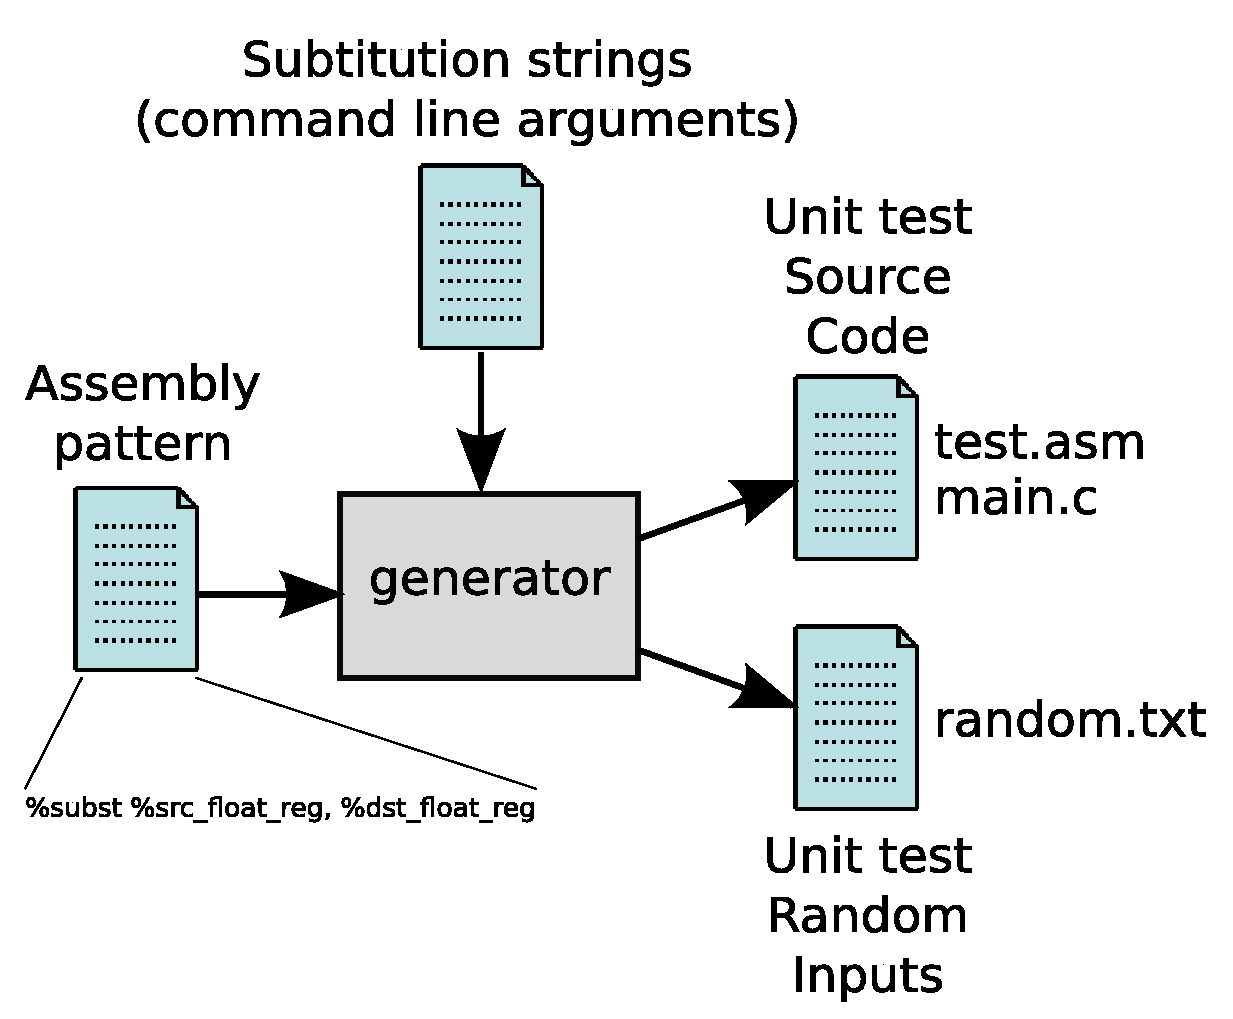
\includegraphics[width=8.0cm]{tms320c3x/fig_unit_test_generator.pdf}
					\caption{\label{fig:tms320c3x_unit_test_generator}UNISIM TMS320C3X unit test generator.}
				\end{center}
			\end{minipage}
			\begin{minipage}{8.0cm}
				\begin{center}
					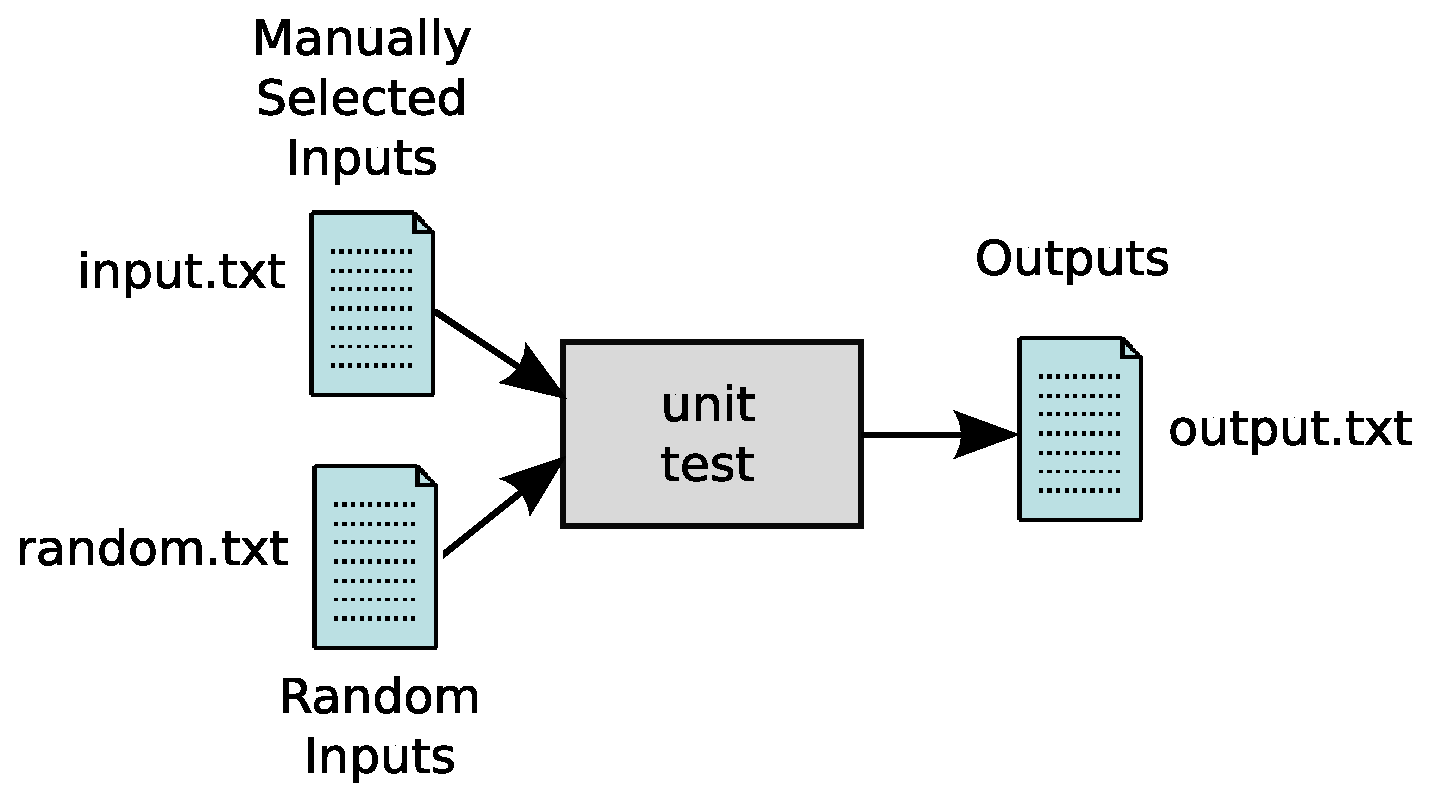
\includegraphics[width=8.0cm]{tms320c3x/fig_unit_test.pdf}
					\caption{\label{fig:tms320c3x_unit_test} A generated unit test.}
				\end{center}
			\end{minipage}
		\end{minipage}
		\vspace{0.5cm}
		\begin{minipage}{\textwidth}
			\begin{center}
				\input{tms320c3x/assembly_pattern}
				\caption{\label{fig:tms320c3x_assembly_pattern} Example of assembly pattern.}
			\end{center}
		\end{minipage}
		\vspace{0.5cm}
		\begin{minipage}{\textwidth}
			\begin{center}
				\tablehead{\hline}
				\tabletail{\hline}
				\begin{supertabular}{|p{16cm}|}
				\multicolumn{1}{|p{16cm}|}{{\scriptsize \texttt{; \it {-}{-}{-}{-}~INPUTS~{-}{-}{-}{-}}\newline
				\texttt{; \it ~r0:~a~32-bit~integer~register}\newline
				\texttt{; \it ~ar2:~an~auxiliary~register~pointing~to~an~array~of~16~32-bit~floating~point~values}\newline
				\texttt{; \it ~r1:~a~32-bit~integer~register~(value~for~st)}\newline
				\texttt{; \it ~r2:~a~40-bit~floating~point~register}\newline
				\texttt{; \it {-}{-}{-}{-}~OUTPUTS~{-}{-}{-}{-}}\newline
				\texttt{; \it ~ar4:~an~auxiliary~register}\newline
				\texttt{; \it ~r2:~a~40-bit~floating~point~register}\newline
				\texttt{; \it ~r3:~a~32-bit~integer~register~(value~of~st)}\newline
				\texttt{~~ldiu~5,~bk~~~~~~~~~~~~~~~~~; \ding{202} \it ~load~block~size~(should~be~at~most~8)}\newline
				\texttt{~~and~5~-~1,~r0~~~~~~~~~~~~~~; \ding{203} \it ~crop~random~value~between~0~and~bk~-~1}\newline
				\texttt{~~ldiu~r0,~ir0~~~~~~~~~~~~~~~; \ding{204} \it ~load~ir0~with~this~random~value}\newline
				\texttt{~~ldiu~ar2,~ar4~~~~~~~~~~~~~~; \ding{205} \it ~load~a~pointer~to~a~buffer~of~16~words}\newline
				\texttt{~~addi~7,~ar4~~~~~~~~~~~~~~~~; \ding{206}}\newline
				\texttt{~~andn~7,~ar4~~~~~~~~~~~~~~~~; \ding{207} \it ~align~circular~buffer~start~on~block~size}\newline
				\texttt{~~ldiu~r1,~st~~~~~~~~~~~~~~~~; \ding{208}}\newline
				\texttt{~~addf~*ar4++(ir0)\%,~r2~~~~~~; \ding{209} \it ~$\leftarrow$~instruction~under~test}\newline
				\texttt{~~ldiu~st,~r3~~~~~~~~~~~~~~~~; \ding{210}}\newline
				\texttt{}}}\\
				\end{supertabular}
				\caption{\label{fig:tms320c3x_generated_assembly} Generated assembly from assembly pattern of Figure~\ref{fig:tms320c3x_assembly_pattern} and substitution strings \texttt{"5"}, \texttt{"7"}, and \texttt{"addf"}.}
			\end{center}
		\end{minipage}
	\end{center}
\end{figure}

The generator needs an assembly pattern and some substitution strings to generate the unit test source code, that is:
\begin{itemize}
\item an assembly function \texttt{unit\_test} (in file \texttt{test.asm}) with the C calling convention and stack parameter passing convention,
\item some random inputs for function \texttt{unit\_test} (\texttt{random.txt}),
\item and a testbench written in C (\texttt{main.c}) that in a loop, reads inputs, calls function \texttt{unit\_test}, and write outputs.
\end{itemize}

An assembly pattern is an assembly source code with special tags. 
These tags start with character \texttt{\%}. 
Most of them represent input/outputs that are substituted by real processor registers during assembly source code generation. 
Tag \texttt{\%subst} is substituted by a substitution string passed as a command line argument to the generator.
Tag \texttt{\%clobber} says to the generator that assembly pattern explicitely clobber register following that tag and that the generator should not allocate that register while substituing inputs and outputs.
Table~\ref{table:tms320c3x_assembly_patterns_tags} lists the available tags.

\begin{table}[p]
\begin{center}
\begin{tabular}{|c|c|l|}
\hline
\textbf{Tag} & \textbf{Type} & \textbf{Storage type}\\
\hline
\texttt{\scriptsize \%src\_int\_reg} & {\scriptsize source} & {\scriptsize 32-bit integer register}\\
\hline
\texttt{\scriptsize \%src\_float\_reg} & {\scriptsize source} & {\scriptsize 40-bit floating-point register}\\
\hline
\texttt{\scriptsize \%src\_aux\_reg} & {\scriptsize source} & {\scriptsize auxiliary register}\\
\hline
\texttt{\scriptsize \%st\_in} & {\scriptsize source} & {\scriptsize 32-bit integer register (value for st)}\\
\hline
\texttt{\scriptsize \%dst\_int\_reg} & {\scriptsize destination} & {\scriptsize 32-bit integer register}\\
\hline
\texttt{\scriptsize \%dst\_float\_reg} & {\scriptsize destination} & {\scriptsize 40-bit floating-point register}\\
\hline
\texttt{\scriptsize \%dst\_aux\_reg} & {\scriptsize destination} & {\scriptsize auxiliary register}\\
\hline
\texttt{\scriptsize \%st\_out} & {\scriptsize destination} & {\scriptsize 32-bit integer register (value of st)}\\
\hline
\texttt{\scriptsize \%src\_dst\_int\_reg} & {\scriptsize source \& destination} & {\scriptsize 32-bit integer register}\\
\hline
\texttt{\scriptsize \%src\_dst\_float\_reg} & {\scriptsize source \& destination} & {\scriptsize 40-bit floating-point register}\\
\hline
\texttt{\scriptsize \%src\_dst\_aux\_reg} & {\scriptsize source \& destination} & {\scriptsize auxiliary register}\\
\hline
\texttt{\scriptsize \%tmp\_int\_reg} & {\scriptsize temporary} & {\scriptsize 32-bit integer register}\\
\hline
\texttt{\scriptsize \%tmp\_float\_reg} & {\scriptsize temporary} & {\scriptsize 40-bit floating-point register}\\
\hline
\texttt{\scriptsize \%tmp\_aux\_reg} & {\scriptsize temporary} & {\scriptsize auxiliary register}\\
\hline
\texttt{\scriptsize \%src\_int\_buf[dim]} & {\scriptsize source} & {\scriptsize auxiliary register pointing to an array of \textit{dim} 32-bit integer values}\\
\hline
\texttt{\scriptsize \%dst\_int\_buf[dim]} & {\scriptsize destination} & {\scriptsize auxiliary register pointing to an array of \textit{dim} 32-bit integer values}\\
\hline
\texttt{\scriptsize \%src\_float\_buf[dim]} & {\scriptsize source} & {\scriptsize auxiliary register pointing to an array of \textit{dim} 32-bit floating-point values}\\
\hline
\texttt{\scriptsize \%dst\_float\_buf[dim]} & {\scriptsize destination} & {\scriptsize auxiliary register pointing to an array of \textit{dim} 32-bit floating-point values}\\
\hline
\texttt{\scriptsize \%subst} & {\scriptsize substitution} & {\scriptsize N/A}\\
\hline
\texttt{\scriptsize \%clobber reg} & {\scriptsize clobber} & {\scriptsize N/A}\\
\hline
\texttt{\scriptsize \%0, \%1, \%2, \ldots} & {\scriptsize reference} & {\scriptsize N/A}\\
\hline
\end{tabular}
\caption{UNISIM TMS320C3X unit test generator assembly patterns tags.}
\label{table:tms320c3x_assembly_patterns_tags}
\end{center}
\end{table}

Figure~\ref{fig:tms320c3x_assembly_pattern} shows an example of assembly pattern and Figure~\ref{fig:tms320c3x_generated_assembly} shows the core of generated assembly. 
During the generation process, each assembly pattern tag is replaced by real processor registers or substitution strings:
\begin{enumerate}
\item[{\large \ding{202}}] \texttt{\%subst} is substituted by integer constant \texttt{5} passed as command line argument of the generator;
\item[{\large \ding{203}}] \texttt{\%0} is substituted as in {\large \ding{202}}, while \texttt{\%src\_int\_reg} is substituted with register \texttt{r0};
\item[{\large \ding{204}}] \texttt{\%clobber ir0} is substituted with register \texttt{ir0} and register \texttt{ir0} is marked as clobbered;
\item[{\large \ding{205}}] \texttt{\%src\_float\_buf[16]} is substituted with register \texttt{ar2} that points to an array of 16 32-bit floating-point values allocated on the stack; \texttt{\%dst\_aux\_reg} is substituted with register \texttt{ar4};
\item[{\large \ding{206}}] \texttt{\%subst} is substituted with integer constant \texttt{7} passed as command line argument to the generator; \texttt{\%6} is substituted as \texttt{\%dst\_aux\_reg} in {\large \ding{205}};
\item[{\large \ding{207}}] \texttt{\%7} is substituted as \texttt{\%subst} in {\large \ding{206}} and \texttt{\%6} is substituted as \texttt{\%dst\_aux\_reg} in {\large \ding{205}};
\item[{\large \ding{208}}] \texttt{\%st\_in} is substituted with register \texttt{r1} and register \texttt{r1} is marked as containing state of register st to enable pretty printing of its content, while \texttt{\%clobber st} is substituted by register \texttt{st} and register \texttt{st} is marked as clobbered;
\item[{\large \ding{209}}] \texttt{\%6} is substituted as \texttt{\%dst\_aux\_reg} in {\large \ding{205}}; \texttt{\%\%} is substituted with \texttt{\%}; \texttt{\%src\_dst\_float\_reg} is substituted with register \texttt{r2};
\item[{\large \ding{210}}] \texttt{\%st\_out} is substituted with register \texttt{r3} and register \texttt{r3} is marked as containing state of register \texttt{st} to enable pretty printing of its content.
\end{enumerate}

The random inputs are obtained with a KISS (Keep It Simple Stupid) random number generator (see \url{http://www.math.niu.edu/\~rusin/known-math/99/RNG}) embedded in the unit tests generator.
The generator creates a uniform distribution for integer numbers. 
Table~\ref{table:tms320c3x_unit_test_float_distribution} shows the distribution for the floating point numbers.

\begin{table}[p]
\begin{center}
\begin{tabular}{|c|c|}
\hline
\textbf{Category} & \textbf{Probability}\\
\hline
-inf & 1/37\\
\hline
smallest negative number & 1/37\\
\hline
zero & 1/37\\
\hline
real zero & 1/37\\
\hline
smallest positive number & 1/37\\
\hline
near to integer & 2/37\\
\hline
+inf & 1/37\\
\hline
small & 2/37\\
\hline
large & 2/37\\ 
\hline
mantissa near previously generated, fully random exponent & 5/37\\
\hline
exponent near previously generated, fully random mantissa & 5/37\\
\hline
float near previously generated & 5/37\\
\hline
fully random & 10/37\\
\hline
\end{tabular}
\caption{UNISIM TMS320C3X unit test generator floating point distribution.}
\label{table:tms320c3x_unit_test_float_distribution}
\end{center}
\end{table}

The unit test source code can be compiled for the development board, and run on both the development board and the UNISIM TMS320C3X simulator.
As a unit test uses the TI C I/O functions, it can reads inputs and write outputs from/to files of the host file system, see Figure~\ref{fig:tms320c3x_unit_test}. 
Such capability has considerably reduced the complexity of testing the assembly pattern under test on both the development board and the UNISIM TMS320C3X simulator.

A unit test reads manually selected inputs from file \texttt{input.txt} and some random generated inputs from file \texttt{random.txt}.
It writes outputs into file \texttt{output.txt}.

\newpage
\subsubsection{The testing environment}
\label{tms320c3x_testing_environment}

A testing environment has been set up using the unit test generator and assembly patterns.
A GNU Makefile is provided to run the unit tests on both the development board (our reference) and the UNISIM TMS320C3X simulator.
The test plan is located in the companion GNU bash script \texttt{factorial.sh}, and more precisely in function '\texttt{factorial}'.
The goal of this function is to generate an auxiliary \texttt{Makefile} (\texttt{Makefile.aux}) that contains building rules of planned unit tests.
A companion C++ program, \texttt{generator} is driven by this auxiliary Makefile to generate the actual unit tests source code.
The generated source code is then compiled for the simulated target using the Texas Instruction cross-compilation tool chain.
The resulting cross-compiled binaries are executed on both a real TMS320C3X DSP using 'Code Composer', and the UNISIM TMS320C3X simulator.
The real/reference execution results and the simulation results are compared, and a failure diagnostic (PASSED or FAILED) is established for each generated unit test program.

As explained in Section~\ref{tms320c3x_unit_tests_generator}, the unit test program output is in file \texttt{output.txt}.
To clearly distinguish simulation results from real execution results, file \texttt{output.txt} (the unit test output) is renamed \texttt{output.ref} when run on the development board or \texttt{output.sim} when run on the UNISIM TMS320C3X simulator.

\noindent The list of supported \texttt{Makefile} targets is the following:

\begin{itemize}
\item \texttt{generator(.exe)}: compile the unit tests generator (\texttt{generator(.exe)})
\item \texttt{compile}: compile the unit tests for the TMS320C3X development board (objects/binaries are \texttt{test.obj}, \texttt{main.obj} and \texttt{test.out})
\item \texttt{rnd}: generate the random input files (\texttt{random.txt}) 
\item \texttt{execute}: execute the unit tests on the TMS320C3X development board (\texttt{EXECUTE} must be set) (execution result is in \texttt{output.ref})
\item \texttt{simulate}: run the simulator (SIMULATE must be set) (simulation results are in \texttt{output.sim})                                    
\item \texttt{check}: compare simulator vs. reference (depends on diff) (check result is in \texttt{output.check})
\item \texttt{diff}: generate difference between simulation vs. reference (depends on \texttt{execute} and \texttt{simulate}) (diff result is in \texttt{output.diff})
\item \texttt{regression-test}: launch a regression test of the UNISIM TMS320C3X simulator
\item \texttt{doc}: generate unit tests documentation (\texttt{unit\_tests.pdf})
\item \texttt{dist}: distribute the testing environment together with reference outputs (\texttt{output.ref})
\item \texttt{clean}: clean everything (but execution results, use \texttt{cleanref} for that)
\item \texttt{cleangen}: clean generator executable (\texttt{generator(.exe)})
\item \texttt{cleansrc}: clean TMS320C3X generated source files (\texttt{test.asm} and \texttt{main.c})
\item \texttt{cleanrnd}: clean generated random input files (\texttt{random.txt})
\item \texttt{cleanbin}: clean TMS320C3X executable files (\texttt{test.out})
\item \texttt{cleanobj}: clean TMS320C3X object files (\texttt{test.obj} and \texttt{main.obj})
\item \texttt{cleangel}: clean GEL scripts (\texttt{run.gel})
\item \texttt{cleansim}: clean simulation results (\texttt{output.sim})
\item \texttt{cleanref}: clean execution results (\texttt{output.ref})
\item \texttt{cleandiff}: clean diff files (\texttt{output.diff})
\item \texttt{cleancheck}: clean check files (\texttt{output.check})
\item \texttt{cleandoc}: clean latex files (\texttt{test.tex})
\end{itemize}

\noindent The following \texttt{Makefile} variables are available for tuning the \texttt{Makefile}:
\begin{itemize}
\item Mandatory:
	\begin{itemize}
	\item \texttt{SIMULATE}: path to the UNISIM TMS320C3X simulator binary
	\item \texttt{EXECUTE}: path to Code Composer executable (i.e. \texttt{cc\_app.exe})
	\item \texttt{DIST\_DIR}: path to destination directory for a distribution
	\end{itemize}
\item Optional:
	\begin{itemize}
	\item \texttt{COMPILER\_PREFIX}: prefix to add before the compiler tools executables names (default: empty)
	\end{itemize}
\end{itemize}

The provided \texttt{Makefile} uses a GNU bash script \texttt{factorial.sh}, that contains a factorial plan, to generate most of the \texttt{Makefile} rules in file \texttt{Makefile.aux}.
To obtain the reference outputs from the developement board, do the following at the command prompt:
\begin{verbatim}
$ make execute EXECUTE=cc_app.exe
\end{verbatim}

Figure~\ref{fig:tms320c3x_cc} shows the testing environment running on Windows and launching unit tests on the development board.

\begin{figure}[!h]
	\begin{center}
		\begin{minipage}{\textwidth}
			\begin{minipage}{9.5cm}
				\begin{center}
					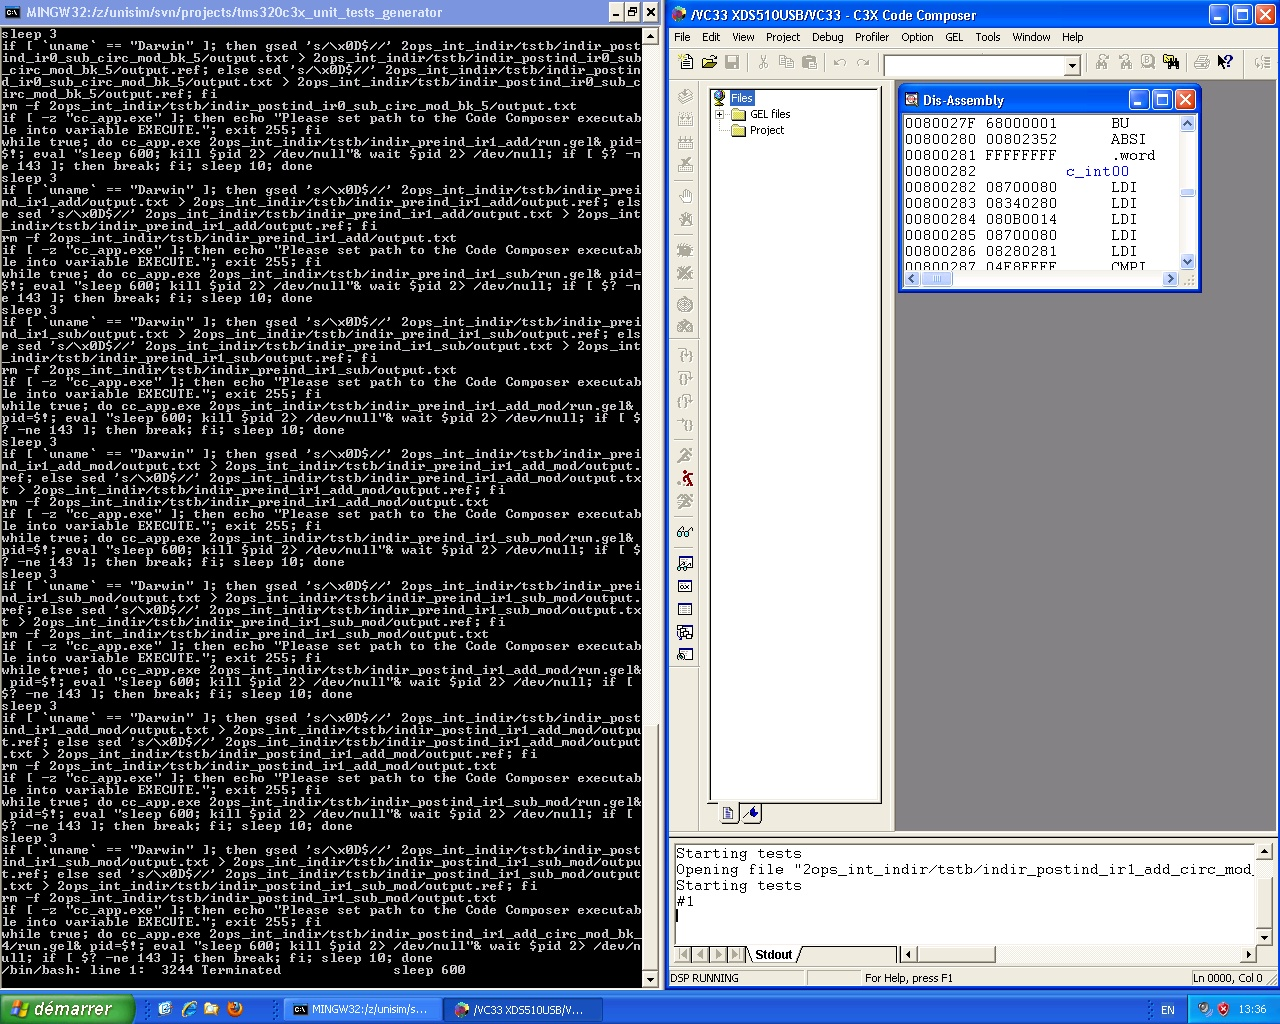
\includegraphics[width=9.0cm]{tms320c3x/fig_code_composer.jpg}
					\caption{\label{fig:tms320c3x_cc} GNU Make (on the left) launching unit tests on the development board using code composer (on the right)}
				\end{center}
			\end{minipage}
			\begin{minipage}{6.5cm}
				\begin{center}
		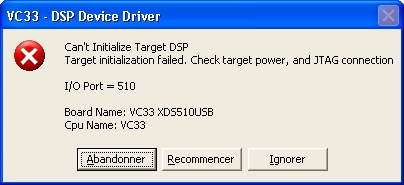
\includegraphics[width=6.0cm]{tms320c3x/fig_driver_error.jpg}
		\caption{\label{fig:tms320c3x_driver_error} VC33 device driver communication problem.}
				\end{center}
			\end{minipage}
		\end{minipage}
	\end{center}
\end{figure}

\textit{Note: You may experience frequent failures of the JTAG Emulator (red LED that indicates activity over USB get stuck), making Code Composer complain in a dialog box that it can't initialize target DSP, see Figure~\ref{fig:tms320c3x_driver_error}. Disconnect and reconnect the USB cable on the JTAG emulator, and then click button "Retry" to resume execution.}

\vspace{0.5cm}

To obtain the simulation outputs from the UNISIM TMS320C3X simulator, do the following at the command prompt:
\begin{verbatim}
$ make simulate SIMULATE=path-to-unisim-tms320c3x-2.0
\end{verbatim}

\subsubsection{Regression tests}
\label{tms320c3x_regression_tests}

The testing environment also acts as a regression test for UNISIM TMS320C3X simulator as the expected results (\texttt{output.ref}) are already provided in the testing environment.

To cross-compile the unit tests programs, do the following at the command prompt on the cross-compilation host:
\begin{verbatim}
$ make generator
$ make compile
$ make c31boot.out
\end{verbatim}

Then to check that all unit tests successfully run on the UNISIM TMS320C3X simulator, do the following at the command prompt on the simulation host:
\begin{verbatim}
$ make cleangen
$ make generator
$ make regression-test SIMULATE=path-to-unisim-tms320c3x-2.0
\end{verbatim}

\noindent The result for each unit test program is either \texttt{PASSED} or \texttt{FAILED}.\\

\textit{Note: At most one instance of the Texas Instrument Cross-compiler can be run at a time (at least on a Windows host and Wine).
Using \texttt{flag -j} of GNU Make when compiling the unit tests programs results in unexpected behaviors.}

\textit{Note: Unit test program \texttt{parallel\_float/stf\_stf/reg\_buf} will likely fail because of a bug in instruction \texttt{STF || STF} in the TMS320VC33 of our development board.}


\chapter{UNISIM Virtex 5 FXT simulator}
\label{virtex5fxt}
\section{Introduction}

\subsection{UNISIM}

UNISIM provides several virtual platforms and a framework to ease the development of new virtual platforms.
A virtual platform is a software tool, often called simulator, that mimics the behavior of an electronic system so that software can run on it before silicon or FPGA implementation of that electronic system is available.
The simulated electronic system can include lots of microprocessors and devices.
Depending on the needed representativeness and simulator development budget, a simulator can be as simple as an instruction set simulator as well as a full system simulator.
A full system simulator, not only executes the microprocessor instruction set, like an instruction set simulator, but also simulates buses, I/O devices, sensors, actuators, so that real application workloads and operating systems can run on them.
Most of UNISIM virtual platforms are full system simulators, which means that they are sufficiently representative of the real hardware that whole operating systems (e.g. Linux, VxWorks), unmodified software stacks (e.g. an AUTOSAR software stack), and industrial applications can run on them.
The UNISIM virtual platforms are modular: a simulator is the assembly of properly configured simulation components (e.g. CPU, RAM, buses).
They are written in C/C++ and based on industry standards, like IEEE1666$^{TM}$, Accellera SystemC$^{TM}$ and Accellera SystemC$^{TM}$ TLM 2.0.

\noindent Some use cases of UNISIM virtual platforms are:
\begin{itemize}
\item Development of SystemC IPs (intellectual property) and new virtual platforms: UNISIM is an open development environment that comprise a SystemC module library, and a set of services (debugging, program loaders, …). It can be a fundation for the development of new SystemC IPs and new virtual virtual platforms.
\item Hybrid virtual platform: UNISIM/SystemC and an FPGA accelerator can be mixed to build some hybrid virtual platforms: for instance simulating processor cores within UNISIM/SystemC, and prototyping specialized IPs/devices within an FPGA accelerator. Hybridization allows using indifferently both UNISIM/SystemC IPs (on a standard host machine) and VHDL IPs (on an FPGA accelerator), but also speeding up simulation of large systems.
\item Non-intrusive debugging and testing of software: It means that, unlike on the real hardware, software can be debugged and tested without affecting either its functional and/or temporal behavior.
With such virtual instrumentation, the user can seamlessly stop and resume execution of software, profile the software, inspect the system status, inject values on the sensors, modify the state of program variables and microprocessor/device registers, and then analyze the result without modifying the software.
\item Hardware/software integration: software stack can be debugged and tested within a representative hardware environment before the availability of either the FPGA prototypes or the real hardware.
The software stack can be composed of low level software (e.g. drivers), of a real-time operating system, and of applications generated from high level models (Papyrus, Matlab Simulink, Statemate Stateflow, …)
\end{itemize}

Several open source virtual platforms for different targets (ARM, PowerPC, Star12X, and TMS320C3X) and different hosts (Linux, Windows, Mac OS X) are available for download here.
These virtual platforms have been evaluated and used in various industry domains such as automotive, avionic, military, electrical equipments for medium tension, nuclear safety.

\subsection{Virtex 5 FXT Simulator}

\begin{figure}[p]
	\begin{center}
		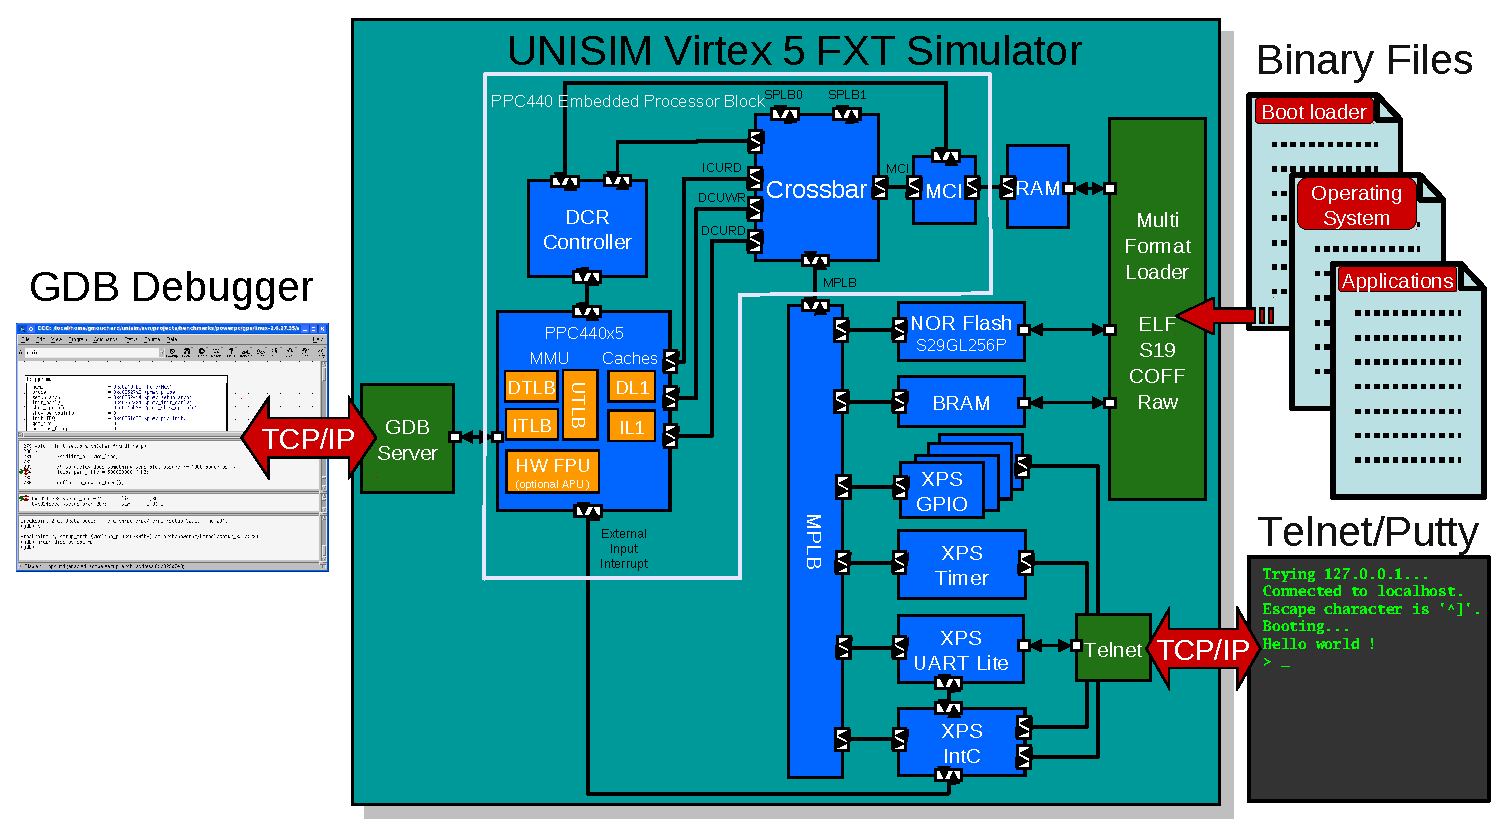
\includegraphics[width=\textwidth]{virtex5fxt/fig_schematic.pdf}
	\end{center}
	\caption{UNISIM Virtex 5 FXT simulator schematic.}
	\label{fig:simulator_schematic}
\end{figure}

\begin{table}[p]
	\begin{center}
		\begin{tabular}{|l|l|l|}
		\hline
		\multicolumn{1}{|c|}{\textbf{Address range}} & \multicolumn{1}{|c|}{\textbf{Component name}} & \multicolumn{1}{|c|}{\textbf{Hardware device}}\\
		\hline
		\texttt{0x00000000-0x0003ffff} & \texttt{ram} & 256 MB RAM\\
		\hline
		\texttt{0x81400000-0x8140ffff} & \texttt{gpio-leds-8bit} & XPS GPIO\\
		\hline
		\texttt{0x81420000-0x8142ffff} & \texttt{gpio-5-leds-positions} & XPS GPIO\\
		\hline
		\texttt{0x81440000-0x8144ffff} & \texttt{gpio-push-buttons-5bit} & XPS GPIO\\
		\hline
		\texttt{0x81460000-0x8146ffff} & \texttt{gpio-dip-switches-8bit} & XPS GPIO\\
		\hline
		\texttt{0x81800000-0x8180ffff} & \texttt{intc} & XPS IntC\\
		\hline
		\texttt{0x83c00000-0x83c0ffff} & \texttt{timer} & XPS Timer/Counter\\
		\hline
		\texttt{0x84000000-0x8400ffff} & \texttt{uart-lite} & XPS UART Lite\\
		\hline
		\texttt{0xfc000000-0xfdffffff} & \texttt{flash} & S29GL256P\\
		\hline
		\texttt{0xfffc0000-0xffffffff} & \texttt{bram} & 256 KB BRAM\\
		\hline
		\end{tabular}
	\end{center}
	\caption{Simulator memory mapping.}
	\label{table:memory_mapping}
\end{table}

The UNISIM Virtex 5 FXT is a virtual platform that tries to mimic a Xilinx ML507 development board that include a Xilinx Virtex 5 FXT (FPGA + PPC440).

\noindent The UNISIM Virtex 5 FXT simulator, which Figure~\ref{fig:simulator_schematic} shows the schematic, implements the following:
\begin{itemize}
	\item PPC440 Embedded Processor Block (UG200~\cite{UG200}):
		\begin{itemize}
			\item All the PPC440x5 \cite{PPC440x5} instruction set of a Xilinx Virtex 5 FXT
			\item Optional FPU that is similar to Xilinx FPU APU \cite{APU_FPU}
			\item PowerPC Book E MMU (shadow ITLB, shadow DTLB, unified TLB)
			\item Caches (instruction and data)
			\item Integrated timers (decrementer, fixed interval, watchdog)
			\item Exception handling mechanisms
			\item DCR (device control register) bus controller
			\item Crossbar
			\item MCI (Memory Controller Interface)
			\item MPLB (master processor local bus) interface
			\item SPLB0 and SPLB1 (slave processor local bus) interfaces
		\end{itemize}
	\item MPLB (master processor local bus) link
	\item 256 MB RAM on MCI
	\item 256 KB BRAM on MPLB
	\item XPS IntC interrupt controller (v2.01a) \cite{XPS_INTC} on MPLB
	\item XPS Timer/Counter (v1.02a) \cite{XPS_TIMER_COUNTER} on MPLB
	\item Spansion 256 Mbits (32 MB) S29GL256P off-chip flash memory \cite{S29GLP} on MPLB
	\item XPS UART Lite (v1.01a) \cite{XPS_UART_LITE} on MPLB
	\item Four XPS GPIO modules (v2.00a) \cite{XPS_GPIO} on MPLB connected to two LED boards and two DIP switch/push buttons boards
\end{itemize}

\noindent Several stub modules are currently integrated in the simulator to test the XPS Timer/Counter module:
\begin{itemize}
\item GenerateOut stubs connected on XPS Timer/Counter « GenerateOut » outputs
\item PWM stub connected on XPS Timer/Counter « PWM0 » output
\item CaptureTrigger stubs (optional randomized outputs) connected on XPS Timer/Counter « CaptureTrigger » inputs
\item SPLB stubs
\item DCR stubs
\end{itemize}

\cleardoublepage

\noindent The simulator also supports the following features :
\begin{itemize}
\item Loading of ELF32, ELF64 \cite{ELF} and Motorola S19 (S-Record) \cite{S19} files
\item An integrated console debugger that supports debugging both at assembly level and source level (e.g. C source code). Source level debugging is only available for ELF binary files including DWARF v2 or v3 \cite{DWARF3} debugging informations
\item Support for the GDB \cite{GDB} serial remote protocol over TCP/IP. That allows debugging a binary running into the simulator at assembly and/or source level using the GNU debugger (aka GDB)
\item Support for a telnet console over the XPS UART Lite
\end{itemize}

Table~\ref{table:memory_mapping} shows the simulator memory mapping.

\noindent The 1.0 release of the simulator is composed of:
\begin{itemize}
\item the simulator source code: unisim-virtex5fxt-1.0beta13.tar.gz
\item the present documentation
\end{itemize}

Please follow the installation instructions in Section~\ref{building_simulator} to get the simulator building on your own building environment.
Section~\ref{getting_started} presents the basics for using the simulator.
Section~\ref{examples_of_use} presents some examples of use of the simulator.
Appendix~\ref{techref} contains the technical references (generated) of the simulator.

\section{Building the simulator}
\label{building_simulator}

\subsection{Requirements}

\noindent The following tools or libraries must be installed:
\begin{itemize}
\item GNU C++ compiler (aka. g++)
\item GNU Flex (aka. flex)
\item GNU Bison (aka. bison)
\item Standard GNU C++ library (aka. libstdc++-dev that comes with g++)
\item Boost (aka. libboost-dev)
\item Editline/Libedit (aka. libedit-dev)
\item zlib (aka. zlib1g-dev)
\item libxml2 (aka. libxml2-dev)
\end{itemize}

\subsection{Installing SystemC 2.3.1}
\subsubsection{Download the source code}
Register at \url{http://www.accellera.org} and then download systemc-2.3.1.tgz from the Accelera SystemC standards download page.

\subsubsection{Uncompressing the source code tarballs}
\begin{script}
   $ tar zxvf systemc-2.3.1.tgz
\end{script}
  
This will uncompress the source of SystemC in directory systemc-2.3.1. 

\subsubsection{Configuring SystemC}
To handle threads, SystemC relies on QuickThreads, a fast implementation of user's threads. QuickThreads speeds-up threads switching compared to the slower kernel POSIX threads and thus considerably improves overall simulation performance. To configure the SystemC building process with the built-in QuickThreads (recommended), do the following at the command prompt:
\begin{script}
   $ cd systemc-2.3.1
   $ mkdir objdir
   $ cd objdir
   $ mkdir ${HOME}/systemc
   $ ../configure --prefix=${HOME}/systemc --disable-shared
\end{script}
However, if you intend to instrument your simulator (e.g. with valgrind) to debug the simulator memory leaks, bad memory accesses, pointers, and uninitialized memory reads, you should use the slower kernel POSIX threads. To configure the SystemC building process with the kernel POSIX threads, do the following at the command prompt:
\begin{script}
   $ cd systemc-2.3.1
   $ mkdir objdir
   $ cd objdir
   $ mkdir ${HOME}/systemc
   $ ../configure --prefix=${HOME}/systemc --enable-pthreads --disable-shared
\end{script}

\subsubsection{Compiling and installing SystemC}
To compile SystemC, do the following at the command prompt:
\begin{script}
   $ make
   $ make install
\end{script}

\subsection{Building the UNISIM Virtex 5 FXT simulator}
\subsubsection{Uncompressing the source code tarball}
\begin{script}
   $ tar zxvf unisim-virtex5fxt-1.0beta13.tar.gz
\end{script}

\subsubsection{Configuring the simulator building process}
\begin{script}
  $ cd unisim-virtex5fxt-1.0beta13
  $ ./configure \
          --with-systemc=${HOME}/systemc
\end{script}

\subsubsection{Compiling the simulator}
\begin{script}
   $ make
\end{script}

\noindent The simulator binaries are in \texttt{virtex5fxt/bin} subdirectory.
The simulators comes in eight flavors in:
\begin{itemize}
\item \texttt{unisim-virtex5fxt-1.0beta13}: release simulator
\item \texttt{unisim-virtex5fxt-wfpu-1.0beta13}: release simulator with a FPU APU
\item \texttt{unisim-virtex5fxt-wfpu-wocache-1.0beta13}: release simulator with a FPU APU but without instruction and data caches
\item \texttt{unisim-virtex5fxt-wocache-1.0beta13}: release simulator without instruction and data caches
\item \texttt{unisim-virtex5fxt-debug-1.0beta13}: development simulator
\item \texttt{unisim-virtex5fxt-wfpu-debug-1.0beta13}: development simulator with a FPU APU
\item \texttt{unisim-virtex5fxt-wfpu-wocache-debug-1.0beta13}: development simulator with a FPU APU but without instruction and data caches
\item \texttt{unisim-virtex5fxt-wocache-debug-1.0beta13}: development simulator without instruction and data caches
\end{itemize}

\section{Cross-compiling the simulator}

This section explains how to build (i.e. cross-compile) the simulator for a host system type (e.g. Windows) from another build system type (e.g. Linux/i386).
The simulator is built on the build machine whereas it will run on the host machine.
In later sub-sections, we consider cross-compiling the simulator for Windows from a Linux distribution using the mingw32 GCC cross-compiler.
Most Linux distributions provide a mingw32 tool chain as a set of packages.
Once installed the mingw32 tool chain binary file names are prefixed with:
\begin{itemize}
\item \texttt{i586-mingw32msvc-} on Ubuntu and Debian Linux distributions
\item \texttt{i686-pc-mingw32-} on RedHat, Fedora, and SUSE Linux distributions
\item \texttt{i586-pc-mingw32-} on Mandriva and Mageia Linux distributions
\end{itemize}
The later sub-sections will refer to the mingw32 tool chain of Ubuntu and Debian Linux distributions.

\subsection{Requirements}

\noindent The following tools must be installed on the Linux build system:
\begin{itemize}
\item GNU C++ cross-compiler for the host system type (aka. i586-mingw32msvc-g++)
\item GNU Flex (aka. flex)
\item GNU Bison (aka. bison)
\item Standard GNU C++ library for the host machine (aka. libstdc++)
\end{itemize}

\subsection{Installing a cross-compiled SystemC 2.3.1}
\subsubsection{Download the source code}
Register at \url{http://www.accellera.org} and then download systemc-2.3.1.tgz from the Accellera SystemC standards download page.

\subsubsection{Uncompressing the source code tarballs}
\begin{script}
   $ tar zxvf systemc-2.3.1.tgz
\end{script}
  
This will uncompress the source of SystemC in directory systemc-2.3.1. 

\subsubsection{Configuring SystemC}
To configure, cross-compile, and install SystemC in your home directory, do the following at the command prompt: 

\begin{script}
   $ cd systemc-2.3.1
   $ mkdir objdir
   $ cd objdir
   $ mkdir ${HOME}/systemc-mingw32
   $ ../configure --prefix=${HOME}/systemc-mingw32 --host=i586-mingw32msvc --disable-shared
\end{script}

\subsubsection{Cross-compiling and installing SystemC}
To cross-compile SystemC, do the following at the command prompt: 
\begin{script}
   $ make
   $ make install
\end{script}

\subsection{Cross-compiling zlib}

Download the source code tarball at \url{http://zlib.net/zlib-1.2.5.tar.gz}.
Uncompress the source code tarball and cross-compile the library:
\begin{script}
   $ tar zxvf zlib-1.2.5.tar.gz
   $ cd zlib-1.2.5
   $ mkdir ${HOME}/zlib-mingw32
   $ make -f win32/Makefile.gcc \
     PREFIX=i586-mingw32msvc- \
     BINARY_PATH=${HOME}/zlib-mingw32/bin \
     INCLUDE_PATH=${HOME}/zlib-mingw32/include \
     LIBRARY_PATH=${HOME}/zlib-mingw32/lib \
     SHARED_MODE=1 install
   $ mv ${HOME}/zlib-mingw32/bin/zdll.a ${HOME}/zlib-mingw32/bin/z.dll.a
\end{script}

\subsection{Cross-compiling libxml2}

Download the source code tarball at \url{ftp://xmlsoft.org/libxml2/libxml2-2.7.8.tar.gz}.
Uncompress the source code tarball and cross-compile the library:
\begin{script}
   $ tar zxvf libxml2-2.7.8.tar.gz
   $ cd libxml2-2.7.8
   $ mkdir ${HOME}/libxml2-mingw32
   $ ./configure  --host=i586-mingw32msvc \
         --without-python --with-zlib=${HOME}/zlib-mingw32 \
          CPPFLAGS='-DLIBXML_STATIC'
   $ make
   $ make install prefix=${HOME}/libxml2-mingw32
\end{script}

\subsection{Cross-compiling Boost}

Download the source code tarball at \url{http://downloads.sourceforge.net/boost/boost\_1\_47\_0.tar.bz2}.
Uncompress the source code tarball and cross-compile the library:

\begin{script}
   $ tar jxvf boost_1_47_0.tar.bz2
   $ cd boost_1_47_0
   $ mkdir ${HOME}/boost-mingw32
   $ ./bootstrap.sh --without-icu
   $ MINGW32_VERSION=$(i586-mingw32msvc-g++ -v 2>&1 | tail -1 | awk '{print $3}' | cut -f 1 -d '-')
   $ echo "using gcc : ${MINGW32_VERSION} :
                 i586-mingw32msvc-g++ :
                 <rc>i586-mingw32msvc-windres
                 <archiver>i586-mingw32msvc-ar
            ;" > user-config.jam
   $ ./bjam toolset=gcc target-os=windows variant=release threading=multi threadapi=win32 \
          link=shared runtime-link=shared --prefix=${HOME}/boost-mingw32 --user-config=user-config.jam \
          --without-mpi --without-python -sNO_BZIP2=1 -sZLIB_BINARY=z.dll \
          -sZLIB_INCLUDE=${HOME}/zlib-mingw32/include -sZLIB_LIBPATH=${HOME}/zlib-mingw32/lib \
          --layout=tagged install
\end{script}

\subsection{Cross-compiling the UNISIM Virtex 5 FXT simulator}
\subsubsection{Uncompressing the source code tarball}
\begin{script}
   $ tar zxvf unisim-virtex5fxt-1.0beta13.tar.gz
\end{script}

\subsubsection{Configuring the simulator building process}
\begin{script}
  $ cd unisim-virtex5fxt-1.0beta13
  $ ./configure.cross \
          --host=i586-mingw32msvc \
          --with-systemc=${HOME}/systemc-mingw32 \
          --with-zlib=${HOME}/zlib-mingw32 \
          --with-libxml2=${HOME}/libxml2-mingw32 \
          --with-boost=${HOME}/boost-mingw32 \
          CXXFLAGS='-O3 -g3 -Wall'
\end{script}

\subsubsection{Cross-compiling the simulator}
\begin{script}
   $ make -f Makefile.cross
\end{script}

\noindent The simulator binaries are in \texttt{virtex5fxt/bin} subdirectory.
The simulators comes in four flavors in:
\begin{itemize}
\item \texttt{unisim-virtex5fxt-1.0beta13.exe}: release simulator without FPU
\item \texttt{unisim-virtex5fxt-wfpu-1.0beta13.exe}: release simulator with FPU
\item \texttt{unisim-virtex5fxt-debug-1.0beta13.exe}: developement simulator
\item \texttt{unisim-virtex5fxt-wfpu-debug-1.0beta13.exe}: developement simulator with FPU
\end{itemize}

The simulator binaries may need some DLLs from mingw32 (e.g. \texttt{libgcc\_s*.dll}) or third party libraries (e.g. \texttt{libxml2-2.dll}).
Place these DLLs in the \texttt{virtex5fxt/bin} subdirectory.
If you prefer not to use DLLs, add \texttt{LDFLAGS=-static} to the \texttt{configure.cross} command line arguments.
The simulator binaries can run natively run on a Windows host system, or an emulated Windows using \texttt{wine} windows emulator.

\section{Getting started}
\label{getting_started}

In this section, we present the basics for using the simulator.
More details are available in Appendix~\ref{techref}.

\subsection{Run-time configuration}

The simulator has a parametrization system that allows configuring individual simulator components, that is the hardware components, and the services.
\noindent The simulator stores its configuration (a set of parameters) in a XML configuration file. 
\newline\\
\noindent The simulator can provide the user with a default XML configuration file with option \texttt{-g}:
\begin{script}
   $ unisim-virtex5fxt-wfpu-1.0beta13 -g default_sim_config.xml
\end{script}

The XML configuration file can be edited, and then reloaded by the simulator with option \texttt{-c}:
\begin{script}
   $ unisim-virtex5fxt-wfpu-1.0beta13 -c sim_config.xml
\end{script}

\noindent The user can also simply set the value of an individual parameter with option \texttt{-s}:
\begin{script}
   $ unisim-virtex5fxt-wfpu-1.0beta13 -s enable-inline-debugger=true
\end{script}

\noindent The simulator can prints the list of parameter set on the console with option \texttt{-l}:
\begin{script}
   $ unisim-virtex5fxt-wfpu-1.0beta13 -l
\end{script}

\noindent In general, each simulator components have log messages that can be switched on or off using a parameter named \texttt{verbose} (or approching):
\begin{script}
   $ unisim-virtex5fxt-wfpu-1.0beta13 -s cpu.verbose-exception=true
\end{script}

\noindent The simulator accepts any combination of the above options.
For example, you can combine these options to change the value of one or more parameters in an XML configuration file:
\begin{script}
   $ unisim-virtex5fxt-wfpu-1.0beta13 -c sim_config.xml -s enable-inline-debugger=true -g sim_config.xml
\end{script}

\subsection{Loading binaries}
\label{loading_binaries}

The simulators has a multi-format loader service that can detect the format of binaries and accordingly instantiate the right loader.
The user can set the list of binary files to load in Parameter loader.filename, each filenames being separated by a comma:
\begin{script}
   $ unisim-virtex5fxt-wfpu-1.0beta13 -s loader.filename='boot.elf,vmlinux,device_tree.dtb,initrd.img'
\end{script}
In the hypothetic case where the multi-format loader would wrongly guess the format of a binary, the user tells the loader what is the format of the binary file:
\begin{script}
   $ unisim-virtex5fxt-wfpu-1.0beta13 \
     -s loader.filename='boot.elf:elf32,vmlinux:elf32,device_tree.dtb:raw,initrd.img:raw'
\end{script}

\noindent If, for any reason (virtual memory, self relocation), the simulator must load a binary file to an address that is not the final address indicated in the binary file itself, the user tells the loader to override (when possible) the base address:
\begin{script}
   $ unisim-virtex5fxt-wfpu-1.0beta13 \
        -s loader.filename='boot.elf,vmlinux,device_tree.dtb,initrd.img' \
        -s loader.file1.base-addr=0 \
        -s loader.file1.force-base-addr=true
\end{script}

If you intend to do "Linux User mode" simulation, that is running a statically linked application binary designed for Linux/PPC440 without actually running Linux/PPC440 within the simulator, as opposed to "full system simulation", you should enable Linux system call translation using command line option "\texttt{--enable-linux-os=1}".

\subsection{Serial console}

The simulator comes with a UART Lite module on MPLB that the target application can use as a serial console.
The simulator telnet service, that is actually a server for the telnet protocol, manages communication between the real network and the virtual UART Lite module.
The combination of the UART Lite module, the telnet service and a serial console aware target application, enables using a real telnet client (running on the host machine or any machine on the internet) as virtual serial console.

To enable the serial console, do the following at the command prompt:
\begin{script}
   $ unisim-virtex5fxt-wfpu-1.0beta13 \
        -s enable-telnet=true \
        -s telnet.telnet-tcp-port=1234
\end{script}

During initialization, the simulator waits for a telnet client connection on the telnet port.
In another console, connect a telnet client to the simulator:
\begin{script}
   $ telnet localhost 1234
\end{script}

At this point, the user can interact with the target application using the telnet client.

\subsection{Using the builtin debugger}

The simulator has an integrated debugger for debugging the target application an a non-intrusive manner.

To enable the inline-debugger, do the following at the command prompt:
\begin{script}
   $ unisim-virtex5fxt-wfpu-1.0beta13 -s enable-inline-debugger=true
\end{script}

The user can enter classical debug commands from the debugger, such as putting breakpoints, watchpoints, stepping instructions, disassembling, dumping memory regions, etc.

To obtain help within the debugger, uses the debugger command \texttt{help}:
\begin{script}
   inline-debugger> help
\end{script}

\subsection{Using a GNU crosstool chain}

\subsubsection{Building a GNU crosstool chain}
\label{building_crosstool_chain}

A crosstool chain is a tool chain to create and manipulate binary programs for a target architecture and operating system (e.g. PowerPC/Linux) that are different from host architecture and operating system (e.g. x86/Linux) that runs the tool chain.
Building a GNU crosstool chain from scratch is a very tedious task.
The process consists of a quite high number of undocumented steps, and mostly relies on the users experience.
Fortunately a community sharing its experience, the crossgcc mailing list, actively supports a tool, crosstool-NG, that considerably simplifies the process of building a crosstool chain.
Xilinx Virtex-5 FXT embedded processor is a PPC440x5 and Xilinx Platform Studio provides a PowerPC hardware FPU.
Hence, from now, we will focus our effort on creating a crosstool chain with GNU GCC 4.7.2 (\texttt{gcc} and \texttt{g++}), GNU C library 2.16.0 (\texttt{glibc}), GNU binutils 2.22 (\texttt{ld}, \texttt{objdump}, and \texttt{readelf}), and GNU GDB 7.4.1 (\texttt{gdb}) for target \texttt{powerpc-440fp-linux-gnu}.

\begin{enumerate}
\item Get crosstool-NG: Download the crosstool-NG archive (e.g crosstool-ng-1.18.0.tar.bz2) from this page: \url{http://crosstool-ng.org}
\item Uncompress crosstool-NG archive:
\begin{script}
   $ tar jxvf crosstool-ng-1.18.0.tar.bz2
\end{script}
\item Configure crosstool-NG build:
\begin{script}
   $ cd crosstool-ng-1.18.0
   $ ./configure --enable-local
\end{script}  
\item Compile crosstool-NG
\begin{script}
   $ make
\end{script}
\item Configure the crosstool chain build as shown on Figure~\ref{fig:ctng_configuration}:
\begin{script}
   $ ./ct-ng menuconfig
\end{script}
\item Build the crosstool chain (this may take tens of minutes/hours):
\begin{script}
   $ ./ct-ng build
\end{script}
\item You crosstool chain is ready in \texttt{\$\{HOME\}/crosstool/powerpc-440fp-linux-gnu}
\end{enumerate}

\begin{figure}[p]
\begin{center}
\begin{script}
Paths and misc options  --->
(${HOME}/crosstool/powerpc-440fp-linux-gnu) Prefix directory

Target options  --->
        Target Architecture (powerpc)  --->
    (440fp) Emit assembly for CPU
    (440fp) Tune for CPU
        Floating point: (hardware (FPU))  --->

Toolchain options  --->
    (440fp) Tuple's vendor string

Operating System  --->
    Target OS (linux)  --->
    Linux kernel version (3.7.3)  --->

Binary utilities  --->
    binutils version (2.22)  --->

C compiler  --->
    gcc version (4.7.2)  --->
    [*] C++
    [ ] Link libstdc++ statically into the gcc binary

C-library  --->
    C library (glibc)  --->
    glibc version (2.16.0)  --->
    (-g) gcc extra flags
    Minimum supported kernel version (Specific kernel version) --->
      Specific kernel version
    (2.6.9) Minimum kernel version to supports

Debug facilities  --->
    [*] gdb  --->

\end{script}
\end{center}
\caption{crosstool chain build configuration (changes from default only) for Crosstool-NG 1.18.0.}
\label{fig:ctng_configuration}
\end{figure}

\cleardoublepage

\subsubsection{Using cross-GCC}

A GCC cross-compiler together with a LD cross-linker can be used to create binaries for the target machine from the host machine:
\begin{script}
   $ ${HOME}/crosstool/powerpc-440fp-linux-gnu/bin/powerpc-440fp-linux-gnu-gcc \
                     nodefaultlibs -nostdlib -mcpu=440fp -c hello.c -o hello.o
   $ ${HOME}/crosstool/powerpc-440fp-linux-gnu/bin/powerpc-440fp-linux-gnu-ld hello.lds -o hello.elf
\end{script}

\noindent Simulator can directly loads such binary files, see Section~\ref{loading_binaries}.

\subsubsection{Using cross-GDB}

GNU GDB client can debug applications running on a remote/local host on the network.
The application is run under the control of program \texttt{gdbserver} while program \texttt{gdb} only manages interactions with the user.
Program \texttt{gdbserver} and \texttt{gdb} communicates over the TCP/IP network using a documented serial remote protocol.
The simulator has a GDB server service that implements the GDB serial remote protocol, so that the simulator can acts as Program \texttt{gdbserver} from the GDB client point of view.

To enable the simulator GDB server, do the following at the command prompt:
\begin{script}
   $ unisim-virtex5fxt-wfpu-1.0beta13 -s enable-gdb-server=true -s gdb-server.tcp-port=1234
\end{script}

During initialization, the simulator waits for a GDB client connection on the GDB server TCP/IP port.
In another console, connect a GDB client to the simulator:
\begin{script}
   $ powerpc-440fp-linux-gnu-gdb boot.elf
   (gdb) target remote :1234
\end{script}

\section{Examples of use}
\label{examples_of_use}

In this section, we present some examples of use for the simulator.
We provide you with scripts and makefiles to build in an automatic manner all the examples.
These examples are available for download in source and binary forms on our web site (\url{http://unisim-vp.org}):
\begin{itemize}
\item Basic system level unit tests: [\href{http://unisim-vp.org/site/downloads/other/benchmarks/virtex5fxt/unisim-virtex5fxt-basic-system-level-unit-tests-bin-v4.tar.gz}{hyperlink to binaries}], [\href{http://unisim-vp.org/site/downloads/other/benchmarks/virtex5fxt/unisim-virtex5fxt-basic-system-level-unit-tests-source-v4.tar.gz}{hyperlink to sources}]
\item MiBench version 1: [\href{http://unisim-vp.org/site/downloads/other/benchmarks/mibench/mibench-v1-bin-powerpc-440fp-linux-gnu-v4.tar.gz}{hyperlink to binaries}], [\href{http://unisim-vp.org/site/downloads/other/benchmarks/mibench/mibench-v1-source-v4.tar.gz}{hyperlink to sources}]
\item light weight Linux distribution: [\href{http://unisim-vp.org/site/downloads/other/benchmarks/linux-distro/unisim-virtex5fxt-linux-distro-bin-v4.tar.gz}{hyperlink to binaries}], [\href{http://unisim-vp.org/site/downloads/other/benchmarks/linux-distro/unisim-virtex5fxt-linux-distro-source-v4.tar.gz}{hyperlink to sources}]
\end{itemize}

To build the examples you need a functional cross tool-chain for Target \texttt{powerpc-440fp-linux-gnu}, see Section~\ref{building_crosstool_chain}.
In later sub-sections, we assume that your cross tool-chain is installed in \texttt{\$\{HOME\}/crosstool/powerpc-440fp-linux-gnu}

\subsection{Basic system level tests}

Table~\ref{table:basic_system_test_summary} shows a summary of basic system level tests.

\begin{table}[h]
	\begin{center}
		\small
		\begin{tabular}{|l|l|l|l|l|l|}
		\hline
		\multicolumn{1}{|c|}{\textbf{Test Name}} &
		\multicolumn{1}{|c|}{\textbf{Directory}} &
		\multicolumn{1}{|c|}{\VROT{\textbf{IntC}}} &
		\multicolumn{1}{|c|}{\VROT{\textbf{Timer}}} &
		\multicolumn{1}{|c|}{\VROT{\textbf{UART Lite}}} &
		\multicolumn{1}{|c|}{\VROT{\textbf{NOR Flash}}}\\
		\hline
		Echo &
		\texttt{\footnotesize xps\_uart\_lite/echo} &
		\X &
		   &
		\X &
		   \\
		\hline
		Poll &
		\texttt{\footnotesize xps\_timer/poll} &
		   &
		\X &
		\X &
		   \\
		\hline
		Gen &
		\texttt{\footnotesize xps\_timer/gen} &
		\X &
		\X &
		\X &
		   \\
		\hline
		Cap &
		\texttt{\footnotesize xps\_timer/cap} &
		\X &
		\X &
		\X &
		   \\
		\hline
		PWM &
		\texttt{\footnotesize xps\_timer/pwm} &
		\X &
		\X &
		\X &
		   \\
		\hline
		Autoselect &
		\texttt{\footnotesize s29gl256p/autoselect} &
		\X &
		   &
		\X &
		\X \\
		\hline
		CFI query &
		\texttt{\footnotesize s29gl256p/cfi\_query} &
		\X &
		   &
		\X &
		\X \\
		\hline
		Chip erase &
		\texttt{\footnotesize s29gl256p/chip\_erase} &
		\X &
		   &
		\X &
		\X \\
		\hline
		Sector erase &
		\texttt{\footnotesize s29gl256p/sector\_erase} &
		\X &
		   &
		\X &
		\X \\
		\hline
		Single word programming &
		\texttt{\footnotesize s29gl256p/single\_word\_programming} &
		\X &
		   &
		\X &
		\X \\
		\hline
		Unlock bypass chip erase &
		\texttt{\footnotesize s29gl256p/unlock\_bypass\_chip\_erase} &
		\X &
		   &
		\X &
		\X \\
		\hline
		Unlock bypass sector erase &
		\texttt{\footnotesize s29gl256p/unlock\_bypass\_sector\_erase} &
		\X &
		   &
		\X &
		\X \\
		\hline
		Unlock bypass word programming &
		\texttt{\footnotesize s29gl256p/unlock\_bypass\_word\_programming} &
		\X &
		   &
		\X &
		\X \\
		\hline
		Write buffer programming &
		\texttt{\footnotesize s29gl256p/write\_buffer\_programming} &
		\X &
		   &
		\X &
		\X \\
		\hline
		\end{tabular}
	\end{center}
	\caption{Summary of basic system level tests.}
	\label{table:basic_system_test_summary}
\end{table}

\subsubsection{Description}

\noindent \textbf{Echo}.The test reads characters from the serial console.
It prints the read characters on the serial console.

\noindent \textbf{Poll}. The test polls the timer/counter \#0.
It prints some of the sampled values on the serial console.

\noindent \textbf{Gen}. The test uses the timer generate mode with interrupt generation every 100 $\mu$s.
It prints the tick of timer on the serial console.

\noindent \textbf{Cap}. The test uses the timer capture mode (randomized input between 1 $\mu$s and 3.995 $\mu$s).
It prints the captured time stamp on the serial console.

\noindent \textbf{PWM}. The test uses the timer in PWM (Pulse Width Modulation) mode with a period of 2 $\mu$s and a duty cycle of 300 ns.

\noindent \textbf{Autoselect}. The test puts the S29GL256P NOR Flash chip in autoselect mode.
It reads the manufacturer and device IDs.
It prints the two IDs on the serial console.
It prints also protection status of each sector.

\noindent \textbf{CFI query}. The test puts the S29GL256P NOR Flash chip in CFI (Common Flash Interface) query mode.
It queries the unique ASCII string "QRY".
For each of the three characters, it prints on the serial console whether they match what is expected ("QRY").

\noindent \textbf{Chip erase}. The test erases the S29GL256P NOR Flash chip.
It checks that all sectors have been erased.

\noindent \textbf{Sector erase}. The test erases the S29GL256P NOR Flash chip, one sector at a time.
It checks that all sectors have been erased.

\noindent \textbf{Single word programming}. The test program a word on the S29GL256P NOR Flash chip.
It verifies that word has been effectively programmed.

\noindent \textbf{Unlock bypass chip erase}. The test erases the S29GL256P NOR Flash chip four times.
It checks that all sectors have been erased.

\noindent \textbf{Unlock bypass sector erase}. The test erases the S29GL256P NOR Flash chip, one sector at a time.
It checks that all sectors have been erased.

\noindent \textbf{Unlock bypass word programming}. The test programs four words in the S29GL256P NOR Flash chip, one word at a time.
It verifies that the four words have beed effectively programmed.

\noindent \textbf{Write buffer programming}. The test programs four words in the S29GL256P NOR Flash chip, using the write buffer.
It verifies that the four words have beed effectively programmed.

\subsubsection{Building the tests}

From the directory where you uncompressed the archive, do the following at the command prompt:
\begin{script}
   $ make CROSS_COMPILE=${HOME}/crosstool/powerpc-440fp-linux-gnu/bin/powerpc-440fp-linux-gnu-
\end{script}

\subsubsection{Running the tests}

\noindent To check in an automatic mannner that the UNISIM Virtex 5 FXT simulator correctly runs the system level unit tests, do the following at the command prompt:
\begin{script}
   $ ./check.sh ${HOME}/unisim-virtex5fxt-1.0beta13/virtex5fxt/bin/unisim-virtex5fxt-wfpu-1.0beta13
\end{script}

\noindent You should get the following output:
\begin{script}
Running xps_timer/poll...done
Running xps_timer/pwm...done
Running xps_timer/gen...done
Running xps_timer/cap...done
Running s29gl256p/single_word_programming...done
Running s29gl256p/unlock_bypass_word_programming...done
Running s29gl256p/cfi_query...done
Running s29gl256p/sector_erase...done
Running s29gl256p/chip_erase...done
Running s29gl256p/autoselect...done
Running s29gl256p/unlock_bypass_sector_erase...done
Running s29gl256p/write_buffer_programming...done
Running s29gl256p/unlock_bypass_chip_erase...done
Running xps_uart_lite/echo...done
xps_timer/poll:PASS
xps_timer/pwm:PASS
xps_timer/gen:PASS
xps_timer/cap:PASS
s29gl256p/single_word_programming:PASS
s29gl256p/unlock_bypass_word_programming:PASS
s29gl256p/cfi_query:PASS
s29gl256p/sector_erase:PASS
s29gl256p/chip_erase:PASS
s29gl256p/autoselect:PASS
s29gl256p/unlock_bypass_sector_erase:PASS
s29gl256p/write_buffer_programming:PASS
s29gl256p/unlock_bypass_chip_erase:PASS
xps_uart_lite/echo:PASS
\end{script}

\cleardoublepage

\subsection{The MiBench version 1 benchmarks}

\subsubsection{Description}
The MiBench~\cite{mibench, mibenchwebsite} version 1 is a free, commercially representative embedded benchmark suite.
Most of the benchmarks come with small and large data sets.
Table~\ref{table:mibench} summarizes the available benchmarks and there current status.
Be aware that some of the benchmarks are so difficult to cross-compile (they were only intended to be natively compiled on the machine that will run them) that we gave up to build them.
Also note that some benchmarks do not run correctly on PowerPC processors because these benchmarks wrongly assumes endian (PowerPC processors natural endian is big-endian whether processors of standard PC are little-endian).
When such limitations exist, they are explained in the status column of the table.

\begin{table}[p]
	\begin{center}
		\begin{tabular}{|l|l|p{5cm}|p{5cm}|}
		\hline
		\multicolumn{1}{|c|}{\textbf{Benchmark}} & \multicolumn{1}{|c|}{\textbf{Category}} & \multicolumn{1}{|c|}{\textbf{Description}} & \multicolumn{1}{|c|}{\textbf{Status}}\\
		\hline
		\texttt{sha} & \texttt{security} & 160-bit secure hash algorithm & OK \\
		\hline
		\texttt{blowfish} & \texttt{security} & Blowfish encryption and decryption & OK \\
		\hline
		\texttt{rijndael} & \texttt{security} & AES encryption and decryption & OK after patching \texttt{aesxam.c} (use \texttt{ftell} instead of \texttt{fgetpos})\\
		\hline
		\texttt{pgp} & \texttt{security} & Asymetric (public key) encryption and decryption & OK \\
		\hline
		\texttt{qsort} & \texttt{automotive} & Sorting algorithm & OK \\
		\hline
		\texttt{susan} & \texttt{automotive} & Corner and edge recognition & OK \\
		\hline
		\texttt{basicmath} & \texttt{automotive} & Solving cubic polynomial, computing integer square root and converting angles & OK \\
		\hline
		\texttt{bitcount} & \texttt{automotive} & Count set bits in integer & OK \\
		\hline
		\texttt{dijkstra} & \texttt{network} & Shortest path in a graph & OK \\
		\hline
		\texttt{FFT} & \texttt{telecomm} & Fast Fourier Transform & OK \\
		\hline
		\texttt{GSM} & \texttt{telecomm} & Global System for Mobile Communications encoder and decoder & OK \\
		\hline
		\texttt{CRC32} & \texttt{telecomm} & 32-bit Cyclic Redundancy Check & OK \\
		\hline
		\texttt{ADPCM} & \texttt{telecomm} & Adaptative Differential Pulse Code Modulation encoder and decoder & OK \\
		\hline
		\texttt{typeset} & \texttt{consumer} & A batch document formatter & OK \\
		\hline
		\texttt{lame} & \texttt{consumer} & MP3 encoder & OK \\
		\hline
		\texttt{mad} & \texttt{consumer} & MPEG audio decoding & Can't get it to cross-compile \\
		\hline
		\texttt{JPEG} & \texttt{consumer} & JPEG encoder and decoder & OK \\
		\hline
		\texttt{tiff} & \texttt{office} & Conversion and Dithering of pictures & Can't get it to cross-compile \\
		\hline
		\texttt{ghostscript} & \texttt{office} & Postscript renderer & Crashes on PowerPC  \\
		\hline
		\texttt{ispell} & \texttt{office} & Spell checker & Fail (input files are endian-sensitive)\\
		\hline
		\texttt{stringsearch} & \texttt{office} & Search for words in text & OK \\
		\hline
		\texttt{rsynth} & \texttt{office} & Text to speech synthesis & OK \\
		\hline
		\texttt{sphinx} & \texttt{office} & Speech decoder & Can't be compiled on modern compilers \\
		\hline
		\end{tabular}
	\end{center}
	\caption{MiBench version 1.0.}
	\label{table:mibench}
\end{table}

\subsubsection{Building the benchmarks}

From the directory where you uncompressed the archive, do the following at the command prompt:
\begin{script}
   $ ./build.sh all powerpc-440fp-linux-gnu ${HOME}/crosstool/powerpc-440fp-linux-gnu
\end{script}

\subsubsection{Running the benchmarks}

The simulator can easily run the MiBench version 1 benchmarks for Linux/PPC440FP without booting Linux.
To do so, the simulator implements a mechanism known as Linux system call translation, also known as User Mode simulation.
It means that a set of Linux system calls are passed through the host operating system, so that it is possible for the loaded applications to access the host file system, read user inputs, and print messages on the console.

\noindent To execute the benchmarks in an automatic manner on a Linux/PPC440FP target machine, do the following at the command prompt:
\begin{script}
   $ ./auto.sh run powerpc-440fp-linux
\end{script}

\noindent To execute the benchmarks in an automatic manner on the UNISIM Virtex 5 FXT simulator, do the following at the command prompt:
\begin{script}
   $ ./auto.sh sim powerpc-440fp-linux \
     ${HOME}/unisim-virtex5fxt-1.0beta13/virtex5fxt/bin/unisim-virtex5fxt-wfpu-1.0beta13
\end{script}

\noindent To check that the results from the PPC440FP target and the simulator match, do the following at the command prompt:
\begin{script}
   $ ./auto.sh check powerpc-440fp-linux ref powerpc-440fp-linux sim
\end{script}

\noindent You should get the following output:
\begin{script}
automotive basicmath large:pass
automotive basicmath small:pass
automotive bitcount large:pass
automotive bitcount small:pass
automotive qsort large:pass
automotive qsort small:pass
automotive susan large:pass
automotive susan small:pass
consumer jpeg large:pass
consumer jpeg small:pass
consumer lame large:pass
consumer lame small:pass
consumer typeset large:pass
consumer typeset small:pass
network dijkstra large:pass
network dijkstra small:pass
network patricia large:pass
network patricia small:pass
office stringsearch large:pass
office stringsearch small:pass
security blowfish large:pass
security blowfish small:pass
security pgp:pass
security rijndael large:pass
security rijndael small:pass
security sha large:pass
security sha small:pass
telecomm adpcm large:pass
telecomm adpcm small:pass
telecomm CRC32 large:pass
telecomm CRC32 small:pass
telecomm FFT large:pass
telecomm FFT small:pass
telecomm gsm large:pass
telecomm gsm small:pass
\end{script}

\subsection{A light weight Linux distribution}

The simulator can easily run a minimalist Linux distribution for a Xilinx Virtex-5 FXT development board.
Table~\ref{table:linux_files} shows the files to load in the simulator to run such a minimalist Linux distribution.
In later sub-sections, we explain how these files are obtained.
We provides you with prebuilt files to allow you quickly boot a minimalist Linux distribution within the simulator.
Go directly to Sub-section~\ref{running_a_linux_distro} if you don't bother about the technique behind creating a light weight Linux distribution for the simulator.
To build such a minimalist Linux distribution, you need a working crosstool chain, see Section~\ref{building_crosstool_chain}.

\begin{table}[!h]
	\begin{center}
		\begin{tabular}{|l|l|l|l|}
		\hline
		\multicolumn{1}{|c|}{\textbf{File}} & \multicolumn{1}{|c|}{\textbf{Start address}} & \multicolumn{1}{|c|}{\textbf{Memory}} & \multicolumn{1}{|c|}{\textbf{Description}}\\
		\hline
		\texttt{boot.elf} & \texttt{0xffff0000} & BRAM & Boot program\\
		\hline
		\texttt{vmlinux} & \texttt{0x00000000} & RAM & Linux kernel\\
		\hline
		\texttt{device\_tree.dtb} & \texttt{0x00800000} & RAM & Device Tree\\
		\hline
		\texttt{initrd.img} & \texttt{0x00900000} & RAM & Initial RAM disk\\
		\hline
		\end{tabular}
	\end{center}
	\caption{Files for booting Linux in the simulator.}
	\label{table:linux_files}
\end{table}

\subsubsection{The boot program}
\label{boot_program}

The boot program is loaded in BRAM which is behind the MPLB.
At reset, the processor starts executing instructions from physical address \texttt{0xfffffffc}.
Thus the boot program is located in memory so that it has an instruction (usually a branch) at that physical address.
The role of the boot program is to initialize early boot and provides the Kernel with some parameters in the processor registers.
Table~\ref{table:linux_register_parameters} shows the registers that needs to be initialized before branching into the Linux Kernel entry point.

\begin{table}[p]
	\begin{center}
		\begin{tabular}{|l|l|}
		\hline
		\multicolumn{1}{|c|}{\textbf{Registers}} & \multicolumn{1}{|c|}{\textbf{Description}}\\
		\hline
		\texttt{r3} & Address of the device tree\\
		\hline
		\texttt{r4} & Start address of the initial RAM disk\\
		\hline
		\texttt{r5} & End address of the initial RAM disk\\
		\hline
		\end{tabular}
	\end{center}
	\caption{Linux kernel register parameters.}
	\label{table:linux_register_parameters}
\end{table}

The boot program, which source is shown on Figure~\ref{fig:boot}, has been designed to make instruction at Label \texttt{start} match the processor start address.
Actually, a branch instructions to elsewhere in the boot program (Label \texttt{init}) is placed at the reset address.
The boot program then starts enabling the MCI (Memory Controller Interface) so that processor can use RAM which is behind the MCI.
It programs the MMU to map the whole 256 MB RAM in the processor address space.
It initializes required register parameters of the Linux kernel, that is the device tree address into Register \texttt{r3}, the initial RAM disk address range into Registers \texttt{r4} and \texttt{r5}, the Linux kernel start address into Register \texttt{SRR0}, and the value of MSR into Register \texttt{SRR1}.
It then branches to the Linux kernel using an \texttt{rfi} instruction (return from interrupt).

\begin{figure}[p]
	\begin{center}
		\input{virtex5fxt/boot}
	\end{center}
	\caption{Boot program (boot.S compiled as boot.elf) loaded in BRAM.}
	\label{fig:boot}
\end{figure}

\subsubsection{The Linux kernel}

The Linux kernel (aka. \texttt{vmlinux}) must be configured and built for the target platform.
\noindent The steps to follow are:
\begin{enumerate}
\item Get the Linux kernel source code: Download the \texttt{linux-3.0.4.tar.bz2} tarball at \url{ftp://ftp.kernel.org/pub/linux/kernel/v3.x/linux-3.0.4.tar.bz2}.
\item Uncompress the tarball
\begin{script}
   $ tar jxvf linux-3.0.4.tar.bz2
\end{script}
\item Before starting configuring the Linux kernel build, we need to modify a Linux configuration file to enable support of hardware FPU.
In File \texttt{arch/powerpc/platforms/44x/Kconfig}, after:
\begin{script}
 config XILINX_VIRTEX_5_FXT
        bool
        select XILINX_VIRTEX
\end{script}
\noindent add the following line:
\begin{script}
        select PPC_FPU
\end{script}
\item We can now configure the Linux kernel build:
\begin{script}
   $ make \
       ARCH=powerpc \
       CROSS_COMPILE=${HOME}/crosstool/powerpc-440fp-linux-gnu/bin/powerpc-440fp-linux-gnu- \
       V=1 menuconfig
\end{script}
The Linux kernel should be configured as shown on Figure~\ref{fig:kernel_configuration}.
Once configuration is finished, at exit don't forget to answer "Yes" when prompted for saving the settings in File \texttt{.config}.
\item The Linux kernel (\texttt{vmlinux}) can now be built.
The build may take tens of minutes.
Do the following at the command prompt:
\begin{script}
   $ make \
       ARCH=powerpc \
       CROSS_COMPILE=${HOME}/crosstool/powerpc-440fp-linux-gnu/bin/powerpc-440fp-linux-gnu- \
       V=1 vmlinux
\end{script}
\end{enumerate}


\begin{figure}[p]
\begin{center}
\begin{script}
Processor support  --->
        Processor Types (AMCC 44x, 46x or 47x)

General Setup  --->
    [*] Initial RAM filesystem and RAM disk (initramfs/initrd) support

Platform support  --->
    [*] Generic Xilinx Virtex 5 FXT board support

Device Drivers  --->
    [*] Block devices  --->
        (16)    Default number of RAM disks
         (65536) Default RAM disk size (kbytes)

        Character devices  --->
            Serial drivers  --->
                <*> Xilinx uartlite serial port support
                [*]   Support for console on Xilinx uartlite serial port

    [*] GPIO Support  --->
        [*] Xilinx GPIO support

    [*] Watchdog Timer Support  --->
        <*> PowerPC Book-E Watchdog Timer

File systems  --->
    <*> Second extended fs support

Kernel hacking  --->
    [*] Compile the kernel with debug info
\end{script}
\end{center}
\caption{Linux kernel configuration (changes from default only).}
\label{fig:kernel_configuration}
\end{figure}

\subsubsection{The device Tree}

On PowerPC embedded platforms, the Linux kernel uses a hierarchical list of devices, namely a device tree where leaves are devices and non-leaf nodes are buses, bridges and interconnects.
It is a rather detailed machine description to allow the Linux kernel to correctly initialize devices and route interrupts to the interrupt routines.
The boot loader or anything else launching the Linux kernel should provide the Linux kernel with the device tree.
Linux provides a device tree compiler that compile a text description (\texttt{.dts} file) in a loadable binary form (\texttt{.dtb} file).
Our example provides user with several device trees, that is one for each initial RAM disk size (6 MB, 8 MB, 12 MB, 16 MB, 24 MB, 32 MB, 64 MB and 96 MB).
The provided device trees are:
\begin{enumerate}
\item \texttt{device-tree-6m.dtb}: device tree for a 6 MB large initial RAM disk
\item \texttt{device-tree-8m.dtb}: device tree for a 8 MB large initial RAM disk
\item \texttt{device-tree-16m.dtb}: device tree for a 16 MB large initial RAM disk
\item \texttt{device-tree-24m.dtb}: device tree for a 24 MB large initial RAM disk
\item \texttt{device-tree-16m.dtb}: device tree for a 16 MB large initial RAM disk
\item \texttt{device-tree-32m.dtb}: device tree for a 32 MB large initial RAM disk
\item \texttt{device-tree-64m.dtb}: device tree for a 64 MB large initial RAM disk
\item \texttt{device-tree-96m.dtb}: device tree for a 96 MB large initial RAM disk
\end{enumerate}

\subsubsection{The initial RAM disk}
The initial RAM disk file is a file containing an image of the root file system.
We consider creating an initial RAM disk with an Ext2 file system in it.
Note that creating an image requires root privileges because mounting a file system requires root privileges.

The steps to follow are:
\begin{enumerate}
\item Create an empty image (\texttt{initrd.img}) of 16 MB:
\begin{script}
   [root@localhost] $ dd if=/dev/zero of=initrd.img count=16384 bs=1024
\end{script}
\item Create an \texttt{Ext2} file system in image:
\begin{script}
   [root@localhost] $ mke2fs -F -m 0 initrd.img
\end{script}
\item Create a mount point and mount image on it:
\begin{script}
   [root@localhost] $ mkdir /media/initrd
   [root@localhost] $ mount -o loop initrd.img /mnt/initrd
\end{script}
\item Now you can directly access withing the image using directory \texttt{/mnt/initrd}. In directory \texttt{/mnt/initrd}, copy every files and directories you want in your image.
\item Unmount image:
\begin{script}
   [root@localhost] $ umount /media/initrd
\end{script}
\end{enumerate}

We provide several prebuilt initial RAM disks.
Some of the initial RAM disks contain a MiBench benchmark (see Table~\ref{table:mibench}) in \texttt{/opt}.
Table~\ref{table:initrd} summarizes the prebuilt initial RAM disks.
\begin{table}[!h]
	\begin{center}
		\begin{tabular}{|l|l|}
		\hline
		\multicolumn{1}{|c|}{\textbf{Initial RAM disk}} & \multicolumn{1}{|c|}{\textbf{Content}}\\
		\hline
		\texttt{initrd.img} & Busybox only\\
		\hline
		\texttt{initrd\_automotive\_basicmath\_large.img} & Busybox + automotive/basicmath (large data set)\\
		\hline
		\texttt{initrd\_automotive\_basicmath\_small.img} & Busybox + automotive/basicmath (small data set)\\
		\hline
		\texttt{initrd\_automotive\_bitcount\_large.img} & Busybox + automotive/bitcount (large data set)\\
		\hline
		\texttt{initrd\_automotive\_bitcount\_small.img} & Busybox + automotive/bitcount (small data set)\\
		\hline
		\texttt{initrd\_automotive\_qsort\_large.img} & Busybox + automotive/qsort (large data set)\\
		\hline
		\texttt{initrd\_automotive\_qsort\_small.img} & Busybox + automotive/qsort (small data set)\\
		\hline
		\texttt{initrd\_automotive\_susan\_large.img} & Busybox + automotive/susan (large data set)\\
		\hline
		\texttt{initrd\_automotive\_susan\_small.img} & Busybox + automotive/susan (small data set)\\
		\hline
		\texttt{initrd\_consumer\_jpeg\_large.img} & Busybox + consumer/JPEG MiBench (large data set)\\
		\hline
		\texttt{initrd\_consumer\_jpeg\_small.img} & Busybox + consumer/JPEG MiBench (small data set)\\
		\hline
		\texttt{initrd\_consumer\_lame\_large.img} & Busybox + consumer/lame (large data set)\\
		\hline
		\texttt{initrd\_consumer\_lame\_small.img} & Busybox + consumer/lame (small data set)\\
		\hline
		\texttt{initrd\_consumer\_typeset\_large.img} & Busybox + consumer/typeset (large data set)\\
		\hline
		\texttt{initrd\_consumer\_typeset\_small.img} & Busybox + consumer/typeset (small data set)\\
		\hline
		\texttt{initrd\_network\_dijkstra\_large.img} & Busybox + network/dijkstra (large data set)\\
		\hline
		\texttt{initrd\_network\_dijkstra\_small.img} & Busybox + network/dijkstra (small data set)\\
		\hline
		\texttt{initrd\_network\_patricia\_large.img} & Busybox + network/patricia (large data set)\\
		\hline
		\texttt{initrd\_network\_patricia\_small.img} & Busybox + network/patricia (small data set)\\
		\hline
		\texttt{initrd\_office\_ghostscript\_large.img} & Busybox + office/ghostscript (large data set)\\
		\hline
		\texttt{initrd\_office\_ghostscript\_small.img} & Busybox + office/ghostscript (small data set)\\
		\hline
		\texttt{initrd\_office\_ispell\_large.img} & Busybox + office/ispell (large data set)\\
		\hline
		\texttt{initrd\_office\_ispell\_small.img} & Busybox + office/ispell (small data set)\\
		\hline
		\texttt{initrd\_office\_rsynth\_large.img} & Busybox + office/rsynth (large data set)\\
		\hline
		\texttt{initrd\_office\_rsynth\_small.img} & Busybox + office/rsynth (small data set)\\
		\hline
		\texttt{initrd\_office\_stringsearch\_large.img} & Busybox + office/stringsearch (large data set)\\
		\hline
		\texttt{initrd\_office\_stringsearch\_small.img} & Busybox + office/stringsearch (small data set)\\
		\hline
		\texttt{initrd\_security\_blowfish\_large.img} & Busybox + security/blowfish (large data set)\\
		\hline
		\texttt{initrd\_security\_blowfish\_small.img} & Busybox + security/blowfish (small data set)\\
		\hline
		\texttt{initrd\_security\_pgp.img} & Busybox + security/PGP\\
		\hline
		\texttt{initrd\_security\_rijndael\_large.img} & Busybox + security/rijndael (large data set)\\
		\hline
		\texttt{initrd\_security\_rijndael\_small.img} & Busybox + security/rijndael (small data set)\\
		\hline
		\texttt{initrd\_security\_sha\_large.img} & Busybox + security/sha (large data set)\\
		\hline
		\texttt{initrd\_security\_sha\_small.img} & Busybox + security/sha (small data set)\\
		\hline
		\texttt{initrd\_telecomm\_adpcm\_large.img} & Busybox + telecomm/ADPCM (large data set)\\
		\hline
		\texttt{initrd\_telecomm\_adpcm\_small.img} & Busybox + telecomm/ADPCM (small data set)\\
		\hline
		\texttt{initrd\_telecomm\_crc32\_large.img} & Busybox + telecomm/CRC32 (large data set)\\
		\hline
		\texttt{initrd\_telecomm\_crc32\_small.img} & Busybox + telecomm/CRC32 (small data set)\\
		\hline
		\texttt{initrd\_telecomm\_fft\_large.img} & Busybox + telecomm/FFT (large data set)\\
		\hline
		\texttt{initrd\_telecomm\_fft\_large.img} & Busybox + telecomm/FFT (small data set)\\
		\hline
		\texttt{initrd\_telecomm\_gsm\_large.img} & Busybox + telecomm/GSM (large data set)\\
		\hline
		\texttt{initrd\_telecomm\_gsm\_small.img} & Busybox + telecomm/GSM (small data set)\\
		\hline
		\end{tabular}
	\end{center}
	\caption{Initial RAM disks.}
	\label{table:initrd}
\end{table}

\cleardoublepage

\subsubsection{Busybox}

Busybox is a light weight shell that includes most of standard UNIX commands. Actually commands are symbolic links to the busybox binary.
Busybox knows which commands to implement looking at its \texttt{argv[0]}.
It is usually a good idea to install Busybox in the initial RAM disk image of an Linux-based embedded platform because it's tiny and easy to cross-compile.
The Linux kernel (\texttt{vmlinux}), at the end of the boot procedure, starts \texttt{linuxrc} located at the root of the root file system (e.g. in an initial RAM disk on device \texttt{/dev/ram0}). Usually \texttt{linuxrc} is a symbolic link to the boot shell (e.g. the Busybox ash shell located at \texttt{/bin/ash}).

\subsubsection{Building the distribution}

From the directory where you uncompressed the archive, do the following at the command prompt:
\begin{script}
   $ ./build.sh all ${HOME}/mibench-v1-source-v3/builds/powerpc-440fp-linux-gnu \
                    ${HOME}/crosstool/powerpc-440fp-linux-gnu
\end{script}

\subsubsection{Booting the distribution}
\label{running_a_linux_distro}

A very small Linux distribution based on Busybox together with a configuration file are provided for the simulator.
To boot that small Linux distribution within the simulator, do the following at the command prompt:

\begin{script}
   $ cd linux_distro
   $ unisim-virtex5fxt-wfpu-1.0beta13 -c config/sim_config.xml
\end{script}

The simulator acts as a telnet server to emulate a terminal over the XPS UART Lite. Once started, it waits for a telnet client connection like \texttt{telnet} or \texttt{PuTTY}.
To connect the telnet client to the simulator, do the following at the command prompt:

\begin{script}
   $ telnet localhost 1234
\end{script}

You can see (in the telnet terminal) the Linux distribution booting in the simulator:
\begin{script}
[    0.000000] Using Xilinx Virtex440 machine description
[    0.000000] Linux version 3.0.4 (unisim-vp@unisim-vp.org) (gcc version 
4.4.6 (crosstool-NG 1.13.2) ) #2 PREEMPT Thu Jan 1 00:00:00 CEST 1970
[    0.000000] Found initrd at 0xc0900000:0xc1900000
[    0.000000] Zone PFN ranges:
[    0.000000]   DMA      0x00000000 -> 0x00001000
[    0.000000]   Normal   empty
[    0.000000] Movable zone start PFN for each node
[    0.000000] early_node_map[1] active PFN ranges
[    0.000000]     0: 0x00000000 -> 0x00001000
[    0.000000] MMU: Allocated 1088 bytes of context maps for 255 contexts
[    0.000000] Built 1 zonelists in Zone order, mobility grouping off.  Total pages: 4094
[    0.000000] Kernel command line: root=/dev/ram0 rw init=linuxrc console=ttyUL0
[    0.000000] PID hash table entries: 1024 (order: -4, 4096 bytes)
[    0.000000] Dentry cache hash table entries: 32768 (order: 1, 131072 bytes)
[    0.000000] Inode-cache hash table entries: 16384 (order: 0, 65536 bytes)
[    0.000000] Memory: 240128k/262144k available (3776k kernel code, 22016k reserved,
 448k data, 620k bss, 256k init)
[    0.000000] Kernel virtual memory layout:
[    0.000000]   * 0xfffd0000..0xffff0000  : fixmap
[    0.000000]   * 0xfde00000..0xfe000000  : consistent mem
[    0.000000]   * 0xfde00000..0xfde00000  : early ioremap
[    0.000000]   * 0xd1000000..0xfde00000  : vmalloc & ioremap
[    0.000000] Preemptible hierarchical RCU implementation.
[    0.000000] NR_IRQS:512
[    0.000000] clocksource: timebase mult[a00000] shift[22] registered
[    0.000000] Console: colour dummy device 80x25
[    0.000343] pid_max: default: 32768 minimum: 301
[    0.000802] Mount-cache hash table entries: 8192
[    0.007581] NET: Registered protocol family 16
[    0.009045] PCI: Probing PCI hardware
[    0.018693] bio: create slab <bio-0> at 0
[    0.019190] XGpio: /plb@0/gpio@81460000: registered
[    0.019403] XGpio: /plb@0/gpio@81400000: registered
[    0.019618] XGpio: /plb@0/gpio@81420000: registered
[    0.019831] XGpio: /plb@0/gpio@81440000: registered
[    0.020361] vgaarb: loaded
[    0.021282] Switching to clocksource timebase
[    0.037828] NET: Registered protocol family 2
[    0.038118] IP route cache hash table entries: 16384 (order: 0, 65536 bytes)
[    0.039300] TCP established hash table entries: 8192 (order: 0, 65536 bytes)
[    0.039638] TCP bind hash table entries: 8192 (order: -1, 32768 bytes)
[    0.039836] TCP: Hash tables configured (established 8192 bind 8192)
[    0.039851] TCP reno registered
[    0.039869] UDP hash table entries: 4096 (order: 0, 65536 bytes)
[    0.040208] UDP-Lite hash table entries: 4096 (order: 0, 65536 bytes)
[    0.041188] NET: Registered protocol family 1
[    0.041734] RPC: Registered named UNIX socket transport module.
[    0.041751] RPC: Registered udp transport module.
[    0.041764] RPC: Registered tcp transport module.
[    0.041778] RPC: Registered tcp NFSv4.1 backchannel transport module.
[    0.041965] Trying to unpack rootfs image as initramfs...
[    0.042228] rootfs image is not initramfs (junk in compressed archive); looks like an initrd
[    0.089044] Freeing initrd memory: 16384k freed
[    0.094043] ROMFS MTD (C) 2007 Red Hat, Inc.
[    0.094294] msgmni has been set to 500
[    0.094696] io scheduler noop registered
[    0.094709] io scheduler deadline registered
[    0.094790] io scheduler cfq registered (default)
[    0.273876] 84000000.serial: ttyUL0 at MMIO 0x84000000 (irq = 19) is a uartlite
[    0.274651] console [ttyUL0] enabled
[    0.282141] brd: module loaded
[    0.286330] loop: module loaded
[    0.286568] Error: Driver 'xsysace' is already registered, aborting...
[    0.286741] xsysace: registration failed; err=-16
[    0.288341] mousedev: PS/2 mouse device common for all mice
[    0.288842] booke_wdt: powerpc book-e watchdog driver loaded
[    0.290497] TCP cubic registered
[    0.290521] NET: Registered protocol family 17
[    0.292335] RAMDISK: ext2 filesystem found at block 0
[    0.292374] RAMDISK: Loading 16384KiB [1 disk] into ram disk... done.
[    0.632474] VFS: Mounted root (ext2 filesystem) on device 1:0.
[    0.632744] Freeing unused kernel memory: 256k init
starting pid 747, tty '': '/etc/init.d/rcS'
starting pid 750, tty '': '/bin/cttyhack /etc/init.sh'


BusyBox v1.19.3 (2012-09-11 13:47:51 CEST) built-in shell (ash)
Enter 'help' for a list of built-in commands.

[/]$
\end{script}

Once the boot is over, you can enter shell commands at the command prompt in the telnet terminal.
For example, you can ask for CPU informations to the Linux kernel by doing the following at the command prompt in the telnet terminal:
\begin{script}
[/]$ cat /proc/cpuinfo
processor       : 0
cpu             : 440 in Virtex-5 FXT
clock           : 400.000000MHz
revision        : 25.18 (pvr 7ff2 1912)
bogomips        : 800.00
timebase        : 400000000
platform        : Xilinx Virtex440
model           : testing
Memory          : 256 MB
[/]$ 
\end{script}

You may also want to try some MiBench benchmarks within that small Linux distribution.
We provide an initial RAM disk for almost each MiBench benchmark and the corresponding simulator configuration file.
\noindent For example, to run the MiBench Lame benchmark (large data set), do the following at the command prompt:

\begin{script}
   $ cd linux_distro
   $ unisim-virtex5fxt-wfpu-1.0beta13 -c config/sim_config_consumer_lame_large.xml
\end{script}

\noindent In another console, connect the telnet client to the simulator:
\begin{script}
   $ telnet localhost 1234
\end{script}

\textit{Note: The UNISIM Virtex 5 FXT Simulator must have the hardware FPU enabled (\texttt{unisim\--virtex5fxt\--wfpu\--1.0beta13}) to run a Linux kernel for \texttt{powerpc\--440fp\--linux\--gnu}.
When the simulator has the hardware FPU disabled (\texttt{unisim\--virtex5fxt\--1.0beta13}, the simulator can only use the Linux kernel for \texttt{powerpc\--440\--linux\--gnu}.}

To check (this may take tens of minutes/hours) in an automatic mannner that the UNISIM Virtex 5 FXT simulator correctly boots Linux and runs the MiBench version 1 benchmarks, do the following at the command prompt:
\begin{script}
   $ ./check.sh ${HOME}/unisim-virtex5fxt-1.0beta13/virtex5fxt/bin/unisim-virtex5fxt-wfpu-1.0beta13 1234
\end{script}
\textit{Note: the Netcat utility (either traditional or BSD version) must be installed}.

\noindent You should get the following output:
\begin{script}
Launching automotive_basicmath_small (job #1 of 35)....ok
Launching automotive_basicmath_large (job #2 of 35)....ok
Launching automotive_bitcount_small (job #3 of 35)....ok
Launching automotive_bitcount_large (job #4 of 35)....ok
Launching automotive_qsort_small (job #5 of 35)....ok
Launching automotive_qsort_large (job #6 of 35)....ok
Launching automotive_susan_small (job #7 of 35)....ok
Launching automotive_susan_large (job #8 of 35)....ok
Launching consumer_jpeg_small (job #9 of 35)....ok
Launching consumer_jpeg_large (job #10 of 35)....ok
Launching consumer_lame_small (job #11 of 35)....ok
Launching consumer_lame_large (job #12 of 35)....ok
Launching consumer_typeset_small (job #13 of 35)....ok
Launching consumer_typeset_large (job #14 of 35)....ok
Launching network_dijkstra_small (job #15 of 35)....ok
Launching network_dijkstra_large (job #16 of 35)....ok
Launching network_patricia_small (job #17 of 35)....ok
Launching network_patricia_large (job #18 of 35)....ok
Launching office_stringsearch_small (job #19 of 35)....ok
Launching office_stringsearch_large (job #20 of 35)....ok
Launching security_blowfish_small (job #21 of 35)....ok
Launching security_blowfish_large (job #22 of 35)....ok
Launching security_pgp (job #23 of 35)....ok
Launching security_rijndael_small (job #24 of 35)....ok
Launching security_rijndael_large (job #25 of 35)....ok
Launching security_sha_small (job #26 of 35)....ok
Launching security_sha_large (job #27 of 35)....ok
Launching telecomm_adpcm_small (job #28 of 35)....ok
Launching telecomm_adpcm_large (job #29 of 35).....ok
Launching telecomm_crc32_small (job #30 of 35)....ok
Launching telecomm_crc32_large (job #31 of 35).....ok
Launching telecomm_fft_small (job #32 of 35)....ok
Launching telecomm_fft_large (job #33 of 35)....ok
Launching telecomm_gsm_small (job #34 of 35)....ok
Launching telecomm_gsm_large (job #35 of 35)....ok
automotive_basicmath_small:PASS
automotive_basicmath_large:PASS
automotive_bitcount_small:PASS
automotive_bitcount_large:PASS
automotive_qsort_small:PASS
automotive_qsort_large:PASS
automotive_susan_small:PASS
automotive_susan_large:PASS
consumer_jpeg_small:PASS
consumer_jpeg_large:PASS
consumer_lame_small:PASS
consumer_lame_large:PASS
consumer_typeset_small:PASS
consumer_typeset_large:PASS
network_dijkstra_small:PASS
network_dijkstra_large:PASS
network_patricia_small:PASS
network_patricia_large:PASS
office_stringsearch_small:PASS
office_stringsearch_large:PASS
security_blowfish_small:PASS
security_blowfish_large:PASS
security_pgp:PASS
security_rijndael_small:PASS
security_rijndael_large:PASS
security_sha_small:PASS
security_sha_large:PASS
telecomm_adpcm_small:PASS
telecomm_adpcm_large:PASS
telecomm_crc32_small:PASS
telecomm_crc32_large:PASS
telecomm_fft_small:PASS
telecomm_fft_large:PASS
telecomm_gsm_small:PASS
telecomm_gsm_large:PASS
\end{script}



\chapter{GenISSLib : An Instruction Set Simulator Generator}
\label{genisslib}
\section{Introduction}

%-------------------------------------------------------------------------
Instruction set simulators are usefull for processor simulation, either
architecture or micro-architecture simulation. Architecture simulation,
also called functional simulation, refers to simulation of the processor
instruction set, whereas micro-architecture simulation refers to components
inside the processor such as pipelines, caches, functional units, branch
predictors. Implementing the instruction set into a software instruction set
simulator is needed for developping and testing software before the target
processor is available or for analyzing softwares without disturbing their execution.
To go from the instruction set specification to a software
implementation of the instruction set, it is convenient to have a description language
for easily describing the instruction encoding, but most description languages
are restricted to only few syntaxical constructions for describing the
instructions behavior. Beside, it is important to have a multipurpose instruction decoder as needs evolves.
GenISSLib is intended for developping such instruction set simulators. It uses a
description language for describing instruction encoding. C++ source code blended with
the description language allow the use of complex instruction behavior, or even more functionalities
like disassembling, binary translation, system calls translation.

\section{Quick Start}

We will now presents you how to use GenISSLib through an example. Suppose that we want to build an instruction set simulator for
a simple 16-bit RISC processor, see table~\ref{instruction_set_summary}. We need GenISSLib to generate C++ class 'Decoder' to decode an instruction, and a C++ class 'Operation' representing the decoded instruction.
class 'Operation' would have a C++ method named 'execute' to execute the instruction, and a C++ method to disassemble the instruction into a string buffer:
\begin{itemize}
	\item \texttt{Operation *Decoder::decode(uint16\_t addr, uint16\_t instruction)}
	\begin{itemize}
		\item \texttt{addr} is the address of the instruction
		\item \texttt{instruction} is the instruction word to decode
		\item \texttt{decode} returns an instance of class \texttt{Operation} containing the decoded instruction
	\end{itemize}
	\item \texttt{void Operation::execute()}
	\item \texttt{void Operation::disasm(uint16\_t pc, char *s)}
	\begin{itemize}
		\item \texttt{pc} is the address of the instruction
		\item \texttt{s} is a string where to disassemble the instruction
	\end{itemize}
\end{itemize}

GenISSLib automatically generates the \texttt{Decoder} class. To ask GenISSLib to generate \texttt{execute} and \texttt{disasm} methods, we have
to declare them using the description language, see figure~\ref{action}. The grammar of the description language is on figure~\ref{grammar}. In the description language, \texttt{execute} and \texttt{disasm} are actions having a prototype.
The action prototype is simply a template for the action. As you can see, the declaration in the instruction set simulator source code directly derives
from these action prototypes. If an instruction is invalid, we can tell GenISSLib to use a default implementation for the action. The default
action implementation for \texttt{execute} is printing \texttt{"Unknown instruction\textbackslash n"} and exit whereas the default action implementation
for \texttt{disasm} is writing a \texttt{"?"} into the string \texttt{s}.

\begin{figure}[ht]
\begin{verbatim}
action {void} execute() {
    printf("Unknown instruction\n");
    exit(-1);
}

action {void} disasm({uint16_t} {pc}, {char *} {s}) {
    sprintf(s, "?");
}
\end{verbatim}
\caption{Declaring the \texttt{execute} and \texttt{disasm} action prototypes.}
\label{action}
\end{figure}

\begin{figure}[h!tb]
	\begin{center}
		\begin{tabular}{|c|c|c|c|c|c|c|c|c|c|c|c|c|c|c|c|c|}
			\hline
			instructions &  15  &  14  &  13  &  12  &  11  &  10  &  ~9  & ~8  &  ~7  &  ~6  &  ~5  &  ~4  &  ~3  &  ~2  &  ~1  &  ~0 \\
			\hline
			add    &   0  &   0  &   0  &   0  & \multicolumn{4}{|c|}{rd} & \multicolumn{4}{|c|}{rs1} & \multicolumn{4}{|c|}{rs2}\\
			\hline
			sub    &   0  &   0  &   0  &   1  & \multicolumn{4}{|c|}{rd} & \multicolumn{4}{|c|}{rs1} & \multicolumn{4}{|c|}{rs2}\\
			\hline
			or     &   0  &   0  &   1  &   0  & \multicolumn{4}{|c|}{rd} & \multicolumn{4}{|c|}{rs1} & \multicolumn{4}{|c|}{rs2}\\
			\hline
			and    &   0  &   0  &   1  &   1  & \multicolumn{4}{|c|}{rd} & \multicolumn{4}{|c|}{rs1} & \multicolumn{4}{|c|}{rs2}\\
			\hline
			not    &   0  &   1  &   0  &   0  & \multicolumn{4}{|c|}{rd}  & \multicolumn{4}{|c|}{rs} &   x  &   x  &   x  &   x \\
			\hline
			shl    &   0  &   1  &   0  &   1  & \multicolumn{4}{|c|}{rd}  & \multicolumn{4}{|c|}{rs} & \multicolumn{4}{|c|}{shamt}\\
			\hline
			shr    &   0  &   1  &   1  &   0  & \multicolumn{4}{|c|}{rd}  & \multicolumn{4}{|c|}{rs} & \multicolumn{4}{|c|}{shamt}\\
			\hline
			load   &   0  &   1  &   1  &   1  & \multicolumn{4}{|c|}{rd}  & \multicolumn{4}{|c|}{base} & \multicolumn{4}{|c|}{index}\\
			\hline
			store  &   1  &   0  &   0  &   0  & \multicolumn{4}{|c|}{rd}  & \multicolumn{4}{|c|}{base} & \multicolumn{4}{|c|}{index}\\
			\hline
			branch &   1  &   0  &   0  &   1  & \multicolumn{12}{|c|}{addr}\\
			\hline
			bne    &   1  &   0  &   1  &   0  & \multicolumn{4}{|c|}{rs} & \multicolumn{8}{|c|}{offset}\\
			\hline
			li     &   1  &   0  &   1  &   1  & \multicolumn{4}{|c|}{rd} & \multicolumn{8}{|c|}{immed}\\
			\hline
		\end{tabular}
		\caption{Instruction Set Summary.}
		\label{instruction_set_summary}
	\end{center}
\end{figure}

\begin{figure}[h!tb]
\begin{center}
	\begin{tabular}{cccccccccccccccc}
		\multicolumn{4}{l}{\Large{\bf{add}}} & \multicolumn{12}{l}{add}\\
		\multicolumn{16}{c}{}\\
		15  &  14  &  13  &  12  &  11  &  10  &  ~9  & ~8  &  ~7  &  ~6  &  ~5  &  ~4  &  ~3  &  ~2  &  ~1  &  ~0 \\
		\hline
			\multicolumn{1}{|c|}{0}  & \multicolumn{1}{|c|}{0} & \multicolumn{1}{|c|}{0} & \multicolumn{1}{|c|}{0} & \multicolumn{4}{|c|}{rd} & \multicolumn{4}{|c|}{rs1} & \multicolumn{4}{|c|}{rs2}\\
		\hline
		\multicolumn{16}{c}{}\\
		\multicolumn{16}{l}{(rd) $\leftarrow$ (rs1) + (rs2)}\\
	\end{tabular}
\end{center}
\caption{The add instruction.}
\label{add_instr}
\end{figure}

\begin{figure}[h!tb]
\begin{center}
\begin{verbatim}
op add(0b0000[4]:rd[4]:rs1[4]:rs2[4])
\end{verbatim}
\label{add_decl}
\caption{declaration of the add operation}
\end{center}
\end{figure}

\begin{figure}[h!tb]
\begin{center}
	\begin{tabular}{cccccccccccccccc}
		\multicolumn{4}{l}{\Large{\bf{not}}} & \multicolumn{12}{l}{negation}\\
		\multicolumn{16}{c}{}\\
		15  &  14  &  13  &  12  &  11  &  10  &  ~9  & ~8  &  ~7  &  ~6  &  ~5  &  ~4  &  ~3  &  ~2  &  ~1  &  ~0 \\
		\hline
		\multicolumn{1}{|c|}{0}  & \multicolumn{1}{|c|}{1} & \multicolumn{1}{|c|}{0} & \multicolumn{1}{|c|}{0} & \multicolumn{4}{|c|}{rd} & \multicolumn{4}{|c|}{rs} & \multicolumn{1}{|c|}{x} & \multicolumn{1}{|c|}{x} & \multicolumn{1}{|c|}{x} & \multicolumn{1}{|c|}{x}\\
		\hline
		\multicolumn{16}{c}{}\\
		\multicolumn{16}{l}{(rd) $\leftarrow$ $~$(rs)}\\
	\end{tabular}
\end{center}
\caption{The not instruction.}
\label{not_instr}
\end{figure}

\begin{figure}[h!tb]
\begin{center}
\begin{verbatim}
op not(0b0100[4]:rd[4]:rs[4]:?[4])
\end{verbatim}
\label{not_decl}
\caption{declaration of the not operation}
\end{center}
\end{figure}

We can now declare instruction encoding and the action implementation with the description language. First, let's consider the add instruction, see figures \ref{add_instr} and \ref{add_decl}: it has a 4-bit opcode
which is 0000 and three 4-bit long operand register numbers encoded into the instruction word which are rd, rs1 and rs2. In the description language \texttt{operation} refers to an instruction.
\texttt{0b0000[4]} refers to the 4-bit opcode, \texttt{rd[4]} to the destination register number which is 4-bit long, \texttt{rs1[4]} and \texttt{rs2[4]} respectively
to the first and second source register numbers. Each bit fields are separated by \texttt{:}. Instead of using binary digits as in \texttt{0b0000[4]}, we can also use decimal digits as in \texttt{0[4]}, or
hexadecimal digits as in \texttt{0x0[4]}.

Now, let's declare the not instruction encoding, see figures \ref{not_instr} and \ref{not_decl}:  it has a 4-bit opcode which is 0001, two 4-bit long operand register numbers which are rd and rs, and 4 don't care bits which can be either 0 or 1.
The 4 don't care bits are represented by \texttt{?[4]} in the declaration of the not operation.

Now, let's implement the actions of the add operation, see figures \ref{add_instr} and \ref{add_impl}. Implementation of an action is just C code.
We can directly use rd, rs1 and rs2 which have been declared in the operation. We use an array (\texttt{gpr}) to represent the registers. The external declaration of that C array can be done anywhere into the description language : we've just added between \{ and \}, the external declarations of \texttt{gpr} and the memory access functions \texttt{mem\_read} and \texttt{mem\_write}, see figure~\ref{c_decl}.

\begin{figure}[h!tb]
\begin{center}
\begin{verbatim}
add.execute = {
    gpr[rd] = gpr[rs1] + gpr[rs2];
}

add.disasm = {
    sprintf(s, "add r%u, r%u, r%u", rd, rs1, rs2);
}
\end{verbatim}
\caption{implementation of the \texttt{execute} and \texttt{disasm} of the add operation.}
\label{add_impl}
\end{center}
\end{figure}

\begin{figure}[ht]
\begin{center}
\begin{verbatim}
{
#include <inttypes.h>
#include <stdio.h>

extern uint16_t cia;
extern uint16_t nia;
extern uint16_t gpr[16];

extern uint16_t mem_read(uint16_t addr);
extern void mem_write(uint16_t addr, uint16_t value);
}
\end{verbatim}
\caption{external declaration of C/C++ variables and functions.}
\label{c_decl}
\end{center}
\end{figure}

\begin{figure}[h!tb]
\begin{center}
	\begin{tabular}{cccccccccccccccc}
		\multicolumn{4}{l}{\Large{\bf{load}}} & \multicolumn{12}{l}{load word}\\
		\multicolumn{16}{c}{}\\
		15  &  14  &  13  &  12  &  11  &  10  &  ~9  & ~8  &  ~7  &  ~6  &  ~5  &  ~4  &  ~3  &  ~2  &  ~1  &  ~0 \\
		\hline
		\multicolumn{1}{|c|}{0}  & \multicolumn{1}{|c|}{1} & \multicolumn{1}{|c|}{1} & \multicolumn{1}{|c|}{1} & \multicolumn{4}{|c|}{rd} & \multicolumn{4}{|c|}{base} & \multicolumn{4}{|c|}{index}\\
		\hline
		\multicolumn{16}{c}{}\\
		\multicolumn{16}{l}{ea $\leftarrow$ (base) + index}\\
		\multicolumn{16}{l}{(rd) $\leftarrow$ Mem[ea]}\\
	\end{tabular}
\end{center}
\caption{The load instruction.}
\label{load_instr}
\end{figure}

Now, let's write the declaration of the load operation, and the implementation of its actions, see figures \ref{load_instr} and \ref{load_decl}: it has a 4-bit index which
must be sign extended and added to a base register to compute the effective address of the load.
Thus we use the \texttt{sext} modifier into the operation declaration. The minimum size in bits of the C variable \texttt{index} holding the \texttt{index} operand field of the operation is supplied between \textless and \textgreater. When decoding a load instruction, GenISSLib will sign extends the \texttt{index} bit field, and store it into the \texttt{index} C variable.

\begin{figure}[h!tb]
\begin{center}
\begin{verbatim}
op load(0b0111[4]:rd[4]:base[4]:sext<16> immed[4])

load.execute = {
    gpr[rd] = mem_read(gpr[base] + immed);
}

load.disasm = {
    sprintf(s, "load r%u, %d(r%u)", rd, immed, base);
}
\end{verbatim}
\caption{The load declaration and implementation.}
\label{load_decl}
\end{center}
\end{figure}

\begin{figure}[h!tb]
\begin{center}
	\begin{tabular}{cccccccccccccccc}
		\multicolumn{4}{l}{\Large{\bf{bne}}} & \multicolumn{12}{l}{conditional branch}\\
		\multicolumn{16}{c}{}\\
		15  &  14  &  13  &  12  &  11  &  10  &  ~9  & ~8  &  ~7  &  ~6  &  ~5  &  ~4  &  ~3  &  ~2  &  ~1  &  ~0 \\
		\hline
		\multicolumn{1}{|c|}{1}  & \multicolumn{1}{|c|}{0} & \multicolumn{1}{|c|}{1} & \multicolumn{1}{|c|}{0} & \multicolumn{4}{|c|}{rs} &\multicolumn{8}{|c|}{offset}\\
		\hline
		\multicolumn{16}{c}{}\\
		\multicolumn{16}{l}{if (rs) \textless \textgreater 0 then}\\
		\multicolumn{1}{l}{} &\multicolumn{15}{l}{NIA $\leftarrow$ CIA + offset}\\
		\multicolumn{16}{l}{else}\\
		\multicolumn{1}{l}{} & \multicolumn{15}{l}{NIA $\leftarrow$ CIA + 1}\\
	\end{tabular}
\end{center}
\caption{The bne instruction.}
\label{bne_instr}
\end{figure}

The implementation of the \texttt{disasm} action of the bne operation uses the \texttt{pc} parameter because we need that the disassembling of the bne instruction contains the target address of the conditional branch, that is \texttt{pc + offset} not \texttt{offset}, see figures \ref{bne_instr} and \ref{bne_decl}.

\begin{figure}[h!tb]
\begin{center}
\begin{verbatim}
op bne(0b1010[4]:rs[4]:sext<16> offset[8])
bne.execute = {
    if(gpr[rs] != 0)
        nia = cia + offset;
}
bne.disasm = {
    sprintf(s, "bne r%u, 0x%04x", rs, pc + offset);
}
\end{verbatim}
\caption{The bne declaration and implementation.}
\label{bne_decl}
\end{center}
\end{figure}

Finally, we uses the generated function to implement the instruction set simulator main loop, see figure~\ref{main}.
We also implement the external function used into the action implementations, see figure~\ref{extern_impl}.

\begin{figure}[h!tb]
\begin{center}
\begin{verbatim}
#include <inttypes.h>"

uint16_t cia;
uint16_t nia;
uint16_t gpr[16];
uint16_t mem[1 << 16];

uint16_t mem_read(uint16_t addr) {
    return mem[addr];
}

void mem_write(uint16_t addr, uint16_t value) {
    mem[addr] = value;
}
\end{verbatim}
\caption{The implementation of the external data and functions.}
\label{extern_impl}
\end{center}
\end{figure}

\begin{figure}[h!tb]
\begin{center}
\begin{verbatim}
#include "risc16.hh"
#include <stdio.h>

int main(int argc, char *argv[]) {
    int i;
    FILE *f;
    uint16_t instruction;
    Operation *operation;
    char disasm_buffer[256];

    cia = 0;
    nia = 0;
    for(i = 0; i < 16; i++) gpr[i] = 0;
    f = fopen("image", "rb");
    fread(mem, 1, sizeof(mem), f);
    fclose(f);
    Decoder decoder;
    for(i = 0; i < 1000; i++)	{
        instruction = mem_read(cia);
        operation = decoder.decode(cia, instruction);
        operation->disasm(cia, disasm_buffer);
        printf("0x%04x: 0x%04x %s\n", cia, instruction,
                                            disasm_buffer);
        nia = cia + 1;
        operation->execute();
        cia = nia;
    }
    return 0;
}
\end{verbatim}
\caption{The main simulation loop.}
\label{main}
\end{center}
\end{figure}



% \begin{figure}[ht]
% \begin{center}
% 	\begin{tabular}{cccccccccccccccc}
% 		\multicolumn{4}{l}{\Large{\bf{sub}}} & \multicolumn{12}{l}{substract}\\
% 		\multicolumn{16}{c}{}\\
% 		15  &  14  &  13  &  12  &  11  &  10  &  ~9  & ~8  &  ~7  &  ~6  &  ~5  &  ~4  &  ~3  &  ~2  &  ~1  &  ~0 \\
% 		\hline
% 			\multicolumn{1}{|c|}{0}  & \multicolumn{1}{|c|}{0} & \multicolumn{1}{|c|}{0} & \multicolumn{1}{|c|}{1} & \multicolumn{4}{|c|}{rd} & \multicolumn{4}{|c|}{rs1} & \multicolumn{4}{|c|}{rs2}\\
% 		\hline
% 		\multicolumn{16}{c}{}\\
% 		\multicolumn{16}{l}{(rd) $\leftarrow$ (rs1) - (rs2)}\\
% 	\end{tabular}
% \end{center}
% \caption{The sub instruction.}
% \label{sub_instr}
% \end{figure}
% 
% \begin{figure}[ht]
% \begin{center}
% 	\begin{tabular}{cccccccccccccccc}
% 		\multicolumn{4}{l}{\Large{\bf{or}}} & \multicolumn{12}{l}{logical or}\\
% 		\multicolumn{16}{c}{}\\
% 		15  &  14  &  13  &  12  &  11  &  10  &  ~9  & ~8  &  ~7  &  ~6  &  ~5  &  ~4  &  ~3  &  ~2  &  ~1  &  ~0 \\
% 		\hline
% 			\multicolumn{1}{|c|}{0}  & \multicolumn{1}{|c|}{0} & \multicolumn{1}{|c|}{1} & \multicolumn{1}{|c|}{0} & \multicolumn{4}{|c|}{rd} & \multicolumn{4}{|c|}{rs1} & \multicolumn{4}{|c|}{rs2}\\
% 		\hline
% 		\multicolumn{16}{c}{}\\
% 		\multicolumn{16}{l}{(rd) $\leftarrow$ (rs1) \textbar (rs2)}\\
% 	\end{tabular}
% \end{center}
% \caption{The or instruction.}
% \label{or_instr}
% \end{figure}
% 
% \begin{figure}[ht]
% \begin{center}
% 	\begin{tabular}{cccccccccccccccc}
% 		\multicolumn{4}{l}{\Large{\bf{and}}} & \multicolumn{12}{l}{logical and}\\
% 		\multicolumn{16}{c}{}\\
% 		15  &  14  &  13  &  12  &  11  &  10  &  ~9  & ~8  &  ~7  &  ~6  &  ~5  &  ~4  &  ~3  &  ~2  &  ~1  &  ~0 \\
% 		\hline
% 			\multicolumn{1}{|c|}{0}  & \multicolumn{1}{|c|}{0} & \multicolumn{1}{|c|}{1} & \multicolumn{1}{|c|}{1} & \multicolumn{4}{|c|}{rd} & \multicolumn{4}{|c|}{rs1} & \multicolumn{4}{|c|}{rs2}\\
% 		\hline
% 		\multicolumn{16}{c}{}\\
% 		\multicolumn{16}{l}{(rd) $\leftarrow$ (rs1) \& (rs2)}\\
% 	\end{tabular}
% \end{center}
% \caption{The and instruction.}
% \label{and_instr}
% \end{figure}
% 
% 
% \begin{figure}[ht]
% \begin{center}
% 	\begin{tabular}{cccccccccccccccc}
% 		\multicolumn{4}{l}{\Large{\bf{shl}}} & \multicolumn{12}{l}{Shift left}\\
% 		\multicolumn{16}{c}{}\\
% 		15  &  14  &  13  &  12  &  11  &  10  &  ~9  & ~8  &  ~7  &  ~6  &  ~5  &  ~4  &  ~3  &  ~2  &  ~1  &  ~0 \\
% 		\hline
% 		\multicolumn{1}{|c|}{0}  & \multicolumn{1}{|c|}{1} & \multicolumn{1}{|c|}{0} & \multicolumn{1}{|c|}{1} & \multicolumn{4}{|c|}{rd} & \multicolumn{4}{|c|}{rs} & \multicolumn{1}{|c|}{x} & \multicolumn{1}{|c|}{x} & \multicolumn{1}{|c|}{x} & \multicolumn{1}{|c|}{x}\\
% 		\hline
% 		\multicolumn{16}{c}{}\\
% 		\multicolumn{16}{l}{(rd) $\leftarrow$ (rs) \textless \textless 1}\\
% 	\end{tabular}
% \end{center}
% \caption{The shl instruction.}
% \label{shl_instr}
% \end{figure}
% 
% \begin{figure}[ht]
% \begin{center}
% 	\begin{tabular}{cccccccccccccccc}
% 		\multicolumn{4}{l}{\Large{\bf{shr}}} & \multicolumn{12}{l}{Shift right}\\
% 		\multicolumn{16}{c}{}\\
% 		15  &  14  &  13  &  12  &  11  &  10  &  ~9  & ~8  &  ~7  &  ~6  &  ~5  &  ~4  &  ~3  &  ~2  &  ~1  &  ~0 \\
% 		\hline
% 		\multicolumn{1}{|c|}{0}  & \multicolumn{1}{|c|}{1} & \multicolumn{1}{|c|}{1} & \multicolumn{1}{|c|}{0} & \multicolumn{4}{|c|}{rd} & \multicolumn{4}{|c|}{rs} & \multicolumn{1}{|c|}{x} & \multicolumn{1}{|c|}{x} & \multicolumn{1}{|c|}{x} & \multicolumn{1}{|c|}{x}\\
% 		\hline
% 		\multicolumn{16}{c}{}\\
% 		\multicolumn{16}{l}{(rd) $\leftarrow$ (rs) \textgreater \textgreater 1}\\
% 	\end{tabular}
% \end{center}
% \caption{The shr instruction.}
% \label{shr_instr}
% \end{figure}
% 
% 
% \begin{figure}[ht]
% \begin{center}
% 	\begin{tabular}{cccccccccccccccc}
% 		\multicolumn{4}{l}{\Large{\bf{store}}} & \multicolumn{12}{l}{store word}\\
% 		\multicolumn{16}{c}{}\\
% 		15  &  14  &  13  &  12  &  11  &  10  &  ~9  & ~8  &  ~7  &  ~6  &  ~5  &  ~4  &  ~3  &  ~2  &  ~1  &  ~0 \\
% 		\hline
% 		\multicolumn{1}{|c|}{1}  & \multicolumn{1}{|c|}{0} & \multicolumn{1}{|c|}{0} & \multicolumn{1}{|c|}{0} & \multicolumn{4}{|c|}{rs} & \multicolumn{4}{|c|}{base} & \multicolumn{4}{|c|}{index}\\
% 		\hline
% 		\multicolumn{16}{c}{}\\
% 		\multicolumn{16}{l}{ea $\leftarrow$ (base) + index}\\
% 		\multicolumn{16}{l}{Mem[ea]  $\leftarrow$ (rs)}\\
% 	\end{tabular}
% \end{center}
% \caption{The store instruction.}
% \label{store_instr}
% \end{figure}
%
% \begin{figure}[ht]
% \begin{center}
% 	\begin{tabular}{cccccccccccccccc}
% 		\multicolumn{4}{l}{\Large{\bf{branch}}} & \multicolumn{12}{l}{unconditional branch}\\
% 		\multicolumn{16}{c}{}\\
% 		15  &  14  &  13  &  12  &  11  &  10  &  ~9  & ~8  &  ~7  &  ~6  &  ~5  &  ~4  &  ~3  &  ~2  &  ~1  &  ~0 \\
% 		\hline
% 		\multicolumn{1}{|c|}{1}  & \multicolumn{1}{|c|}{0} & \multicolumn{1}{|c|}{0} & \multicolumn{1}{|c|}{1} & \multicolumn{12}{|c|}{addr}\\
% 		\hline
% 		\multicolumn{16}{c}{}\\
% 		\multicolumn{16}{l}{NIA $\leftarrow$ addr}\\
% 	\end{tabular}
% \end{center}
% \caption{The branch instruction.}
% \label{branch_instr}
% \end{figure}

\newpage

\section{Technical Reference}

\begin{figure}[p]
input $\rightarrow$ decl\_list\\
decl\_list $\rightarrow$ $\epsilon$ \textbar~~decl\_list decl {\bf $\hookleftarrow$}\\
decl $\rightarrow$ $\epsilon$ \textbar~~op\_decl \textbar~~action\_proto\_decl \textbar~~action\_decl \textbar~~source\_code\_decl \textbar~~include\_decl\\
source\_code\_decl $\rightarrow$ {\bf source\_code}\\
op\_decl $\rightarrow$ {\bf op} {\bf identifier} {\bf (} bitfield\_list {\bf )}\\
bitfield\_list $\rightarrow$ bitfield \textbar~ bitfield\_list {\bf :} bitfield\\
bitfield $\rightarrow$ {\bf integer} {\bf [} {\bf integer} {\bf ]} \textbar~ sext\_modifier size\_modifier {\bf identifier} {\bf [} {\bf integer} {\bf ]} \textbar~ ? {\bf [} {\bf integer}�{\bf ]}\\
sext\_modifier $\rightarrow$ $\epsilon$ \textbar~ {\bf sext}\\
size\_modifier $\rightarrow$ $\epsilon$ \textbar~ {\bf \textless}~ {\bf integer} {\bf \textgreater}~ \textbar~ {\bf \textless}~ {\bf \textgreater}~\\
action\_proto\_decl $\rightarrow$ static\_modifier {\bf action} {\bf source\_code} {\bf identifier} {\bf (} params {\bf )} {\bf source\_code}\\
params $\rightarrow$ $\epsilon$ \textbar~ {\bf source\_code}\\
static\_modifier $\rightarrow$ $\epsilon$ \textbar~ {\bf static}\\
action\_decl $\rightarrow$ {\bf identifier} {\bf.} {\bf identifier} {\bf =} {\bf source\_code}\\
include\_decl $\rightarrow$ {\bf include} {\bf string}\\
\\
{\bf source\_code} is C++ source between \{ and \}\\
{\bf identifier} is an alphanumeric identifier\\
{\bf integer} is a positive integer either binary, decimal or hexadecimal\\
{\bf string} is a double-quoted character string\\
C ( /* */) et C++ ( // ) comments are allowed anywhere.
\caption{The description language grammar.}
\label{grammar}
\end{figure}


\chapter{TLM/TTLM}
\label{tlm_ttlm}
\section{TLM Interface}
\label{tlm_interface}

The proposed TLM interface has a single method called \texttt{Send},
see~Figure~\ref{fig:interface1}. An initiator calls \texttt{Send} to
initiate a transaction with a target. \texttt{Send} is non-blocking:
it means that \texttt{Send} must not call the SystemC
\texttt{wait} primitive. Method \texttt{Send} returns a boolean to
indicate to the initiator if the target can serve the request. If
\texttt{Send} has failed, the initiator should retry it later. Target
method \texttt{Send} takes a reference to the message as argument, not
a copy, so that both initiator and target can share the message. The
message contains three things: the request, the response, and an
event. The initiator puts the request in the message before calling
\texttt{Send}. If any response to the request is expected, the
initiator puts an event in the message, and waits while the target
puts the response in the message, and notifies the event embedded in
the message (not necessarily before returning from \texttt{Send}).
The initiator should not check the response before the target has
notified the embedded event. The request and response types are
specified as template parameters of class TlmMessage.

% Transaction REQ, RSP
% Nonblocking
% Return value (wait)

% \begin{figure}[h]
%   \begin{center}
%     \includegraphics[width=13.0cm]{liberty_handshaking.eps}
%     \caption{\label{fig:liberty_handshaking} Contrat de communication de l'environnement LSE de Liberty.}
%   \end{center}
% \end{figure}

\begin{figure}[h]
  \begin{center}
    \input{tlm/interface1}
    \caption{\label{fig:interface1} TLM interface (simplified).}
  \end{center}
\end{figure}

\subsection{Drawbacks \& Programming facilities: Pointer and event stack}
\label{drawbacks_and_programming_facilities}

% Two problems to solve:
% - message dissapears because send is nonblocking (write example).

\textbf{Message sharing drawbacks}. Sharing the message avoids
unecessary data movements between the initiator and the target, thus
speeding up simulation, but it can complexify the task of the
initiator's writer. The message and especially the request must stay
alive until the target actually uses it. For instance, if the initiator
request does not imply a target response, the initiator can not
deallocate (either in the stack or the heap) the message once the
\texttt{Send} has returned . A simple example of a such behavior is a
write request without acknowledge served by a memory, i.e. the target.
The initiator does not need to wait for a response from the memory,
but still cannot deallocate the message until the memory has
effectively written back the data. The problem is that the initiator's
writer can't know when the message can be freed, unless the
programmer has a well understanding of the complete simulator, thus
knwowing the behavior of each simulator module.

\textbf{Simplifying message sharing}. To symplify the task of the
initiator's writer, a light-weight garbage collector is provided to
the programmer handling automatic deallocation of memory resources,
i.e. the message, once it is no longer used by other modules. The
garbage collector has a fast memory allocator and keeps track of alive
reference to the objects with a reference counter. The object
reference counter is incremented each time a reference to the object
is created, and decremented each time a reference to the object dies.
A class \texttt{Pointer} representing a reference to an object has
been added. The class \texttt{Pointer} is responsible for incrementing
and decrementing the reference counter and calling the garbage
collector once the objects can effectively be freed. A fast allocator
for object pointed by an instance of class \texttt{Pointer} is
provided to the programmer through an overloaded \texttt{new} C++
operator. This overloaded \texttt{new} operator takes an argument which
is the instance of class \texttt{Pointer} holding the object
reference. An example of use is presented
on~Figure~\ref{fig:new_operator}. An integer is allocated using the
overloaded \texttt{new} operator, then initialized to value
\texttt{1}. A pointer is created and initialized to point to the newly
allocated integer.

\begin{figure}[h]
  \begin{center}
    \input{tlm/new_operator}
    \caption{\label{fig:new_operator} Example of use of class
      \texttt{Pointer} and the overloaded \texttt{new} C++ operator.}
  \end{center}
\end{figure}

The reference to the message has been replaced in the TLM interface by
this special pointer, see~Figure~\ref{fig:interface2}. Members
\texttt{req} and \texttt{rsp} have been replaced by this special
pointer too.

\begin{figure}[h]
  \begin{center}
    \input{tlm/interface2}
    \caption{\label{fig:interface2} TLM interface (simplified with
      garbage collector).}
  \end{center}
\end{figure}

% - chaining communication steps.

\begin{figure}[h]
  \begin{center}
    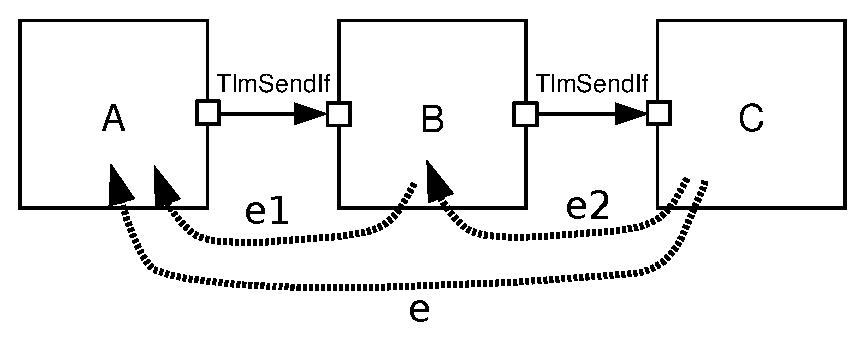
\includegraphics[width=10.0cm]{tlm/chaining_communication_steps.pdf}
    \caption{\label{fig:chaining_communication_steps} Chaining communication steps.}
  \end{center}
\end{figure}

\textbf{Chaining communication steps}. Most of the time a single event
is sufficient for a simple communication scheme. Sometimes several
communication steps are needed before the message actually reachs the
target. For instance, consider an intermediate module is placed
between the initiator and the target,
see~Figure~\ref{fig:chaining_communication_steps}.  Module~A is an
initiator. Module~B is both a target and an initiator. Module~C is a
target. The time spent in module~B affects the total transaction time
between initiator module~A and final target module~C. While the time
spent when processing the transition of the message from A-B to B-C
can be easily computed in module~B \texttt{Send} method, if a single
event is used, the computation of the time spent when the response
goes through B can not be computed, because the response will be
directly notified from module~C to module~A. To account for this
additional delay, only one event is not sufficient. Actually, an
additional event is needed to make module~B wait module~C, while
module~A still waits the target module, which is module~B not
module~C. A stack of events has been introduced to simplify the
programming of chained communication steps. Such communication schemes
are quite common in networks, where intermediate modules would be
switches. Before sending a message, an initiator puts both the request
and the event into the message. Actually, the event is pushed on a
stack. After the \texttt{Send}, the initiator still waits for the
event it has pushed on the stack. Once the event is notified, the
initiator is unblocked and can do a pop on the stack to remove its
event. The TLM interface has been updated to add support for an event
stack, see~Figure~\ref{fig:interface3} (note that access methods to
the stack of events have been omitted from the Figure).

\begin{figure}[h]
  \begin{center}
    \input{tlm/interface3}
    \caption{\label{fig:interface3} TLM interface (with an event stack).}
  \end{center}
\end{figure}

\section{Untimed TLM}
\label{sec:untimed_tlm}

\begin{figure}[h]
  \begin{center}
    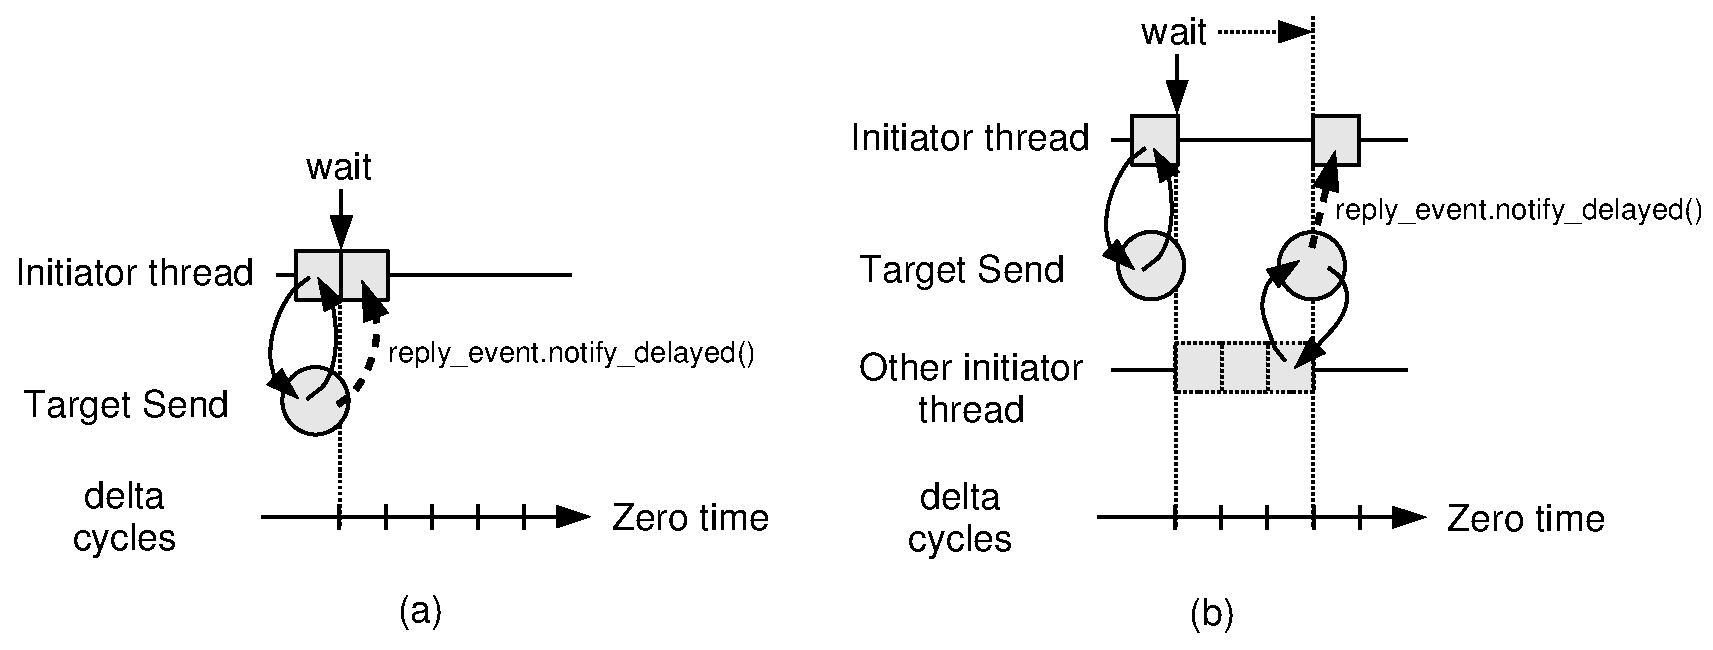
\includegraphics[width=\textwidth]{tlm/utlm_principle.pdf}
    \caption{\label{fig:utlm_principle} Untimed TLM: principle.}
  \end{center}
\end{figure}

This section will demonstrate the use of the TLM interface and message
to design untimed TLM models. In an Untimed TLM (UTLM) model, the
delays for serving requests is not considered,
see~Figure~\ref{fig:utlm_principle}. The simulated time is stuck to
zero and only delta cycles occur during simulation. The initiator
calls target method \texttt{Send} to make the target serve the
request. If the initiator waits for a response, i.e. waits for the
response event, the target triggers the response event for the next
delta cycle, see Figure~\ref{fig:utlm_principle}~(a). While making the initiator wait the response
  event may seem not necessary for untimed models, actually it is necessary
  because the target method \texttt{Send} may not trigger the response
  event before leaving control to the caller initiator thread
  but in another delta cycle. For example, the target may need to receive a
  message from another module to set the response and trigger the
  response event, see Figure~\ref{fig:utlm_principle}~(b).
  As a side effect, forcing this design methodology facilitates the untimed
  and timed models cosimulation, and enables a smooth transition from untimed models to
  timed models.

Consider the example of a system
with one processor and one memory: the processor is an initiator
whereas the memory is a target. Examples of request and response are
provided on Figure~\ref{fig:memory_req_rsp}. The processor can send
\texttt{READ} or \texttt{WRITE} requests to the memory. When the
request is a write, \texttt{MemoryRequest} member \texttt{write\_data}
helds the data to write.

\begin{figure}[p]
\begin{minipage}{\textwidth}
  \begin{center}
    \input{tlm/memory_req_rsp}
    \caption{\label{fig:memory_req_rsp} Example of memory request \& response.}
  \end{center}
\end{minipage}
\begin{minipage}{\textwidth}
~\vspace{3.0cm}
\end{minipage}
\begin{minipage}{\textwidth}
  \begin{center}
    \input{tlm/utlm_memory}
    \caption{\label{fig:utlm_memory} Example of UTLM memory module.}
  \end{center}
\end{minipage}
\end{figure}

A source code example for the processor is provided on
Figure~\ref{fig:utlm_processor}. The processor module has only one
SystemC thread: \texttt{Run}. Thread \texttt{Run} calls
\texttt{PerformRead} and \texttt{PerformWrite} member methods. These
two methods do memory requests using SystemC port \texttt{port}. The
\texttt{PerformRead} operation is the following:

\begin{enumerate}
\item[{\large \ding{202}}] a memory request is allocated;
\item[{\large \ding{203}}] a message is allocated, and initialized
  with the request and the response event;
\item[{\large \ding{204}}] the request is filled;
\item[{\large \ding{205}}] the message is sent using port method
  \texttt{Send}; \texttt{Send} is retried until it has
  succeeded;
\item[{\large \ding{206}}] if \texttt{Send} has failed, the processor
  waits for one delta cycle before actually retrying \texttt{Send};
\item[{\large \ding{207}}] once \texttt{Send} has succeeded, the
  processor waits for the response event;
\item[{\large \ding{208}}] once \texttt{wait} is finished, the
  processor can use the response.
\end{enumerate}

The \texttt{PerformWrite} operation is the following:
\begin{enumerate}
\item[{\large \ding{202}}] a memory request is allocated;
\item[{\large \ding{203}}] a message is allocated, and initialized
  with the request and the response event;
\item[{\large \ding{204}}] the request is filled;
\item[{\large \ding{205}}] the message is sent using port
  \texttt{Send} methods; \texttt{Send} is retried until it has
  succeeded;
\item[{\large \ding{206}}] if \texttt{Send} has failed, the processor
  waits for one delta cycle before actually retrying \texttt{Send};
\end{enumerate}

When \texttt{Send} fails and the processor has to wait for a delta
cycle before retrying (see item {\large \ding{206}} from the previous
operations), the programmer should use a private event to first notify
using \texttt{notify\_delayed} SystemC method and after that, perform
the \texttt{wait}, which effectively provoques a one delta cycle wait.
% We will see later, that \texttt{notify\_delayed} is only necessary
% when writing UTLM models, but not necessary for TTLM models.

\begin{figure}[p]
  \begin{center}
    \input{tlm/utlm_processor}
    \caption{\label{fig:utlm_processor} Example of UTLM processor
      module.}
  \end{center}
\end{figure}

A source code example for the memory is provided on
Figure~\ref{fig:utlm_memory}. The memory module has no thread. The
memory requests are directly served by memory method \texttt{Send}
within the processor module thread. Member method \texttt{Send}
operation is the following:

\begin{enumerate}
\item[{\large \ding{202}}] the request is taken from the message;
\item[{\large \ding{203}}] the response is allocated;
\item[{\large \ding{204}}] if the request is a \texttt{READ}, the
  reponse is filled with the read data; the response is put in the
  message and the response event is notified for the next delta cycle;
\item[{\large \ding{205}}] if the request is a \texttt{WRITE}, the
  data to write is written back in the memory.
\end{enumerate}


\section{Timed TLM}
\label{sec:timed_tlm}

\begin{figure}[h]
  \begin{center}
    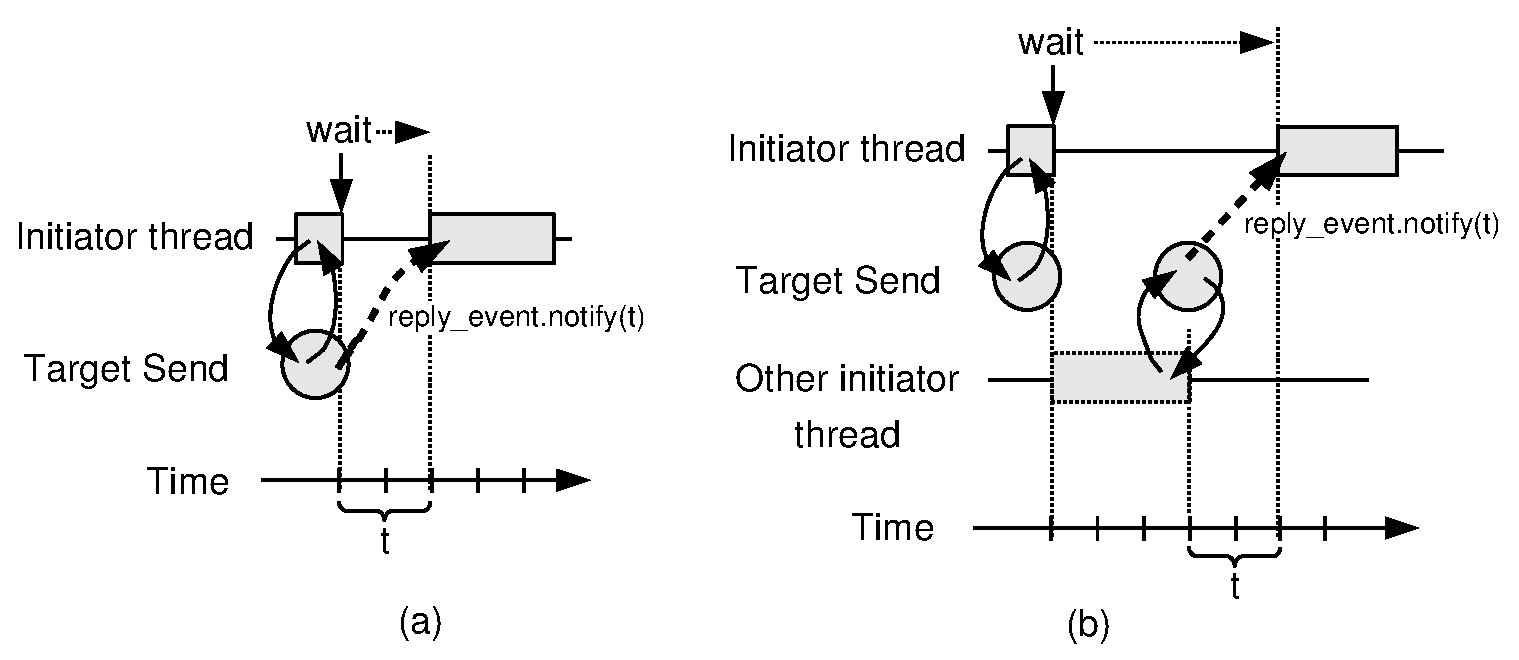
\includegraphics[width=\textwidth]{tlm/ttlm_principle.pdf}
    \caption{\label{fig:ttlm_principle} Timed TLM: principle.}
  \end{center}
\end{figure}

In this section, the use of the TLM interface and message with time
(TTLM) will be demonstrated on several examples with an increasing
complexity. The first example presents how to add time to the untimed
model using one-to-one communication scheme, see
section~\ref{sec:untimed_tlm}. The next example presents a N-to-M
communication scheme using a router between the processors and the
memory, and applying contention over the processors requests. The last
example presents an N-to-M communication scheme using a router between
the processors and the memories, and applying contention over
processors requests and memories responses. As several
processors/memories compete for accessing to the router, the router is
using an arbitration algorithm.  The arbitration algorithm assigns a
fixed time slot to each processor/memory.

In the proposed model the initiator must place itself in the right
time when sending a request, i.e., calling the \texttt{Send} method.
For that purpose, the initiator must use the \texttt{wait} method.
When the target needs to reply to a request the \texttt{notify} method
is used over the response event with the estimated time taken by the
target, see Figure~\ref{fig:ttlm_principle}. The target module
  can trigger the response event when executing the \texttt{Send}
  method, i.e., in the initiator thread, see
  Figure~\ref{fig:ttlm_principle}~(a); or during another cycle (or
  delta cycle), for example, the target module may need that another
  initiator module sends a message to it before triggering the first
  initiator response event, see Figure~\ref{fig:ttlm_principle}~(b).
Note that unlike in the UTLM model \texttt{notify\_delayed} is no
longer needed, unless the notification takes zero time.

\subsection{Example: Simple Model}
The modifications to the UTLM example to make it TTLM are minimal.
Processor and memory now have time parameters among their template
parameters (i.e., \texttt{FREQUENCY} and \texttt{READ\_CYCLES}), which
are used to compute the processor and memory processing times.

The main modification in the processor module is the substitution and
addition of calls to the SystemC primitive \texttt{wait} with time,
see {\large \ding{202}} and {\large \ding{203}} on
Figure~\ref{fig:ttlm_processor}\footnote{This implementation is
  innefficient, because a call to the \texttt{wait} method is done
  (that is, a SystemC synchronization) for each executed instruction.
  Better implementations can be done, but this is not the objective of
  this example.}. For example, it is used when trying to send a
read/write request, and the request fails, see {\large \ding{202}} on
Figure~\ref{fig:ttlm_processor}.  Another use is to advance the
internal clock of the module after an instruction execution, see
{\large \ding{203}} on Figure~\ref{fig:ttlm_processor}.

To convert the memory module to a TTLM module, we have only modified
the call to the \texttt{notify} method, see {\large \ding{202}} on
Figure~\ref{fig:ttlm_memory}, to indicate the time the memory needs to
set the response, the response delay time. Note that the memory sets
the response before notifying it, and that the response could be used
before the delay time, however the module that receives the response
should never suppose so, i.e., another implementation of the memory
could have wait the delay time before setting the response and simply
make a \texttt{notify\_delayed} to make it available.

\begin{figure}[p]
  \begin{center}
    \input{tlm/ttlm_processor}
    \caption{\label{fig:ttlm_processor} Example of TTLM processor.}
  \end{center}
\end{figure}

\begin{figure}[p]
\begin{minipage}{\textwidth}
  \begin{center}
    \input{tlm/ttlm_memory}
    \caption{\label{fig:ttlm_memory} Example of TTLM memory.}
  \end{center}
\end{minipage}
\begin{minipage}{\textwidth}
~\vspace{2.5cm}
\end{minipage}
\begin{minipage}{\textwidth}
  \begin{center}
    \input{tlm/ttlm_router}
    \caption{\label{fig:ttlm_router} Untimed implementation of the
      \texttt{router} module.}
  \end{center}
\end{minipage}
\end{figure}


\subsection{Example: Request contention}
\label{subsec:example_request_contention}

\begin{figure}[h]
  \begin{center}
    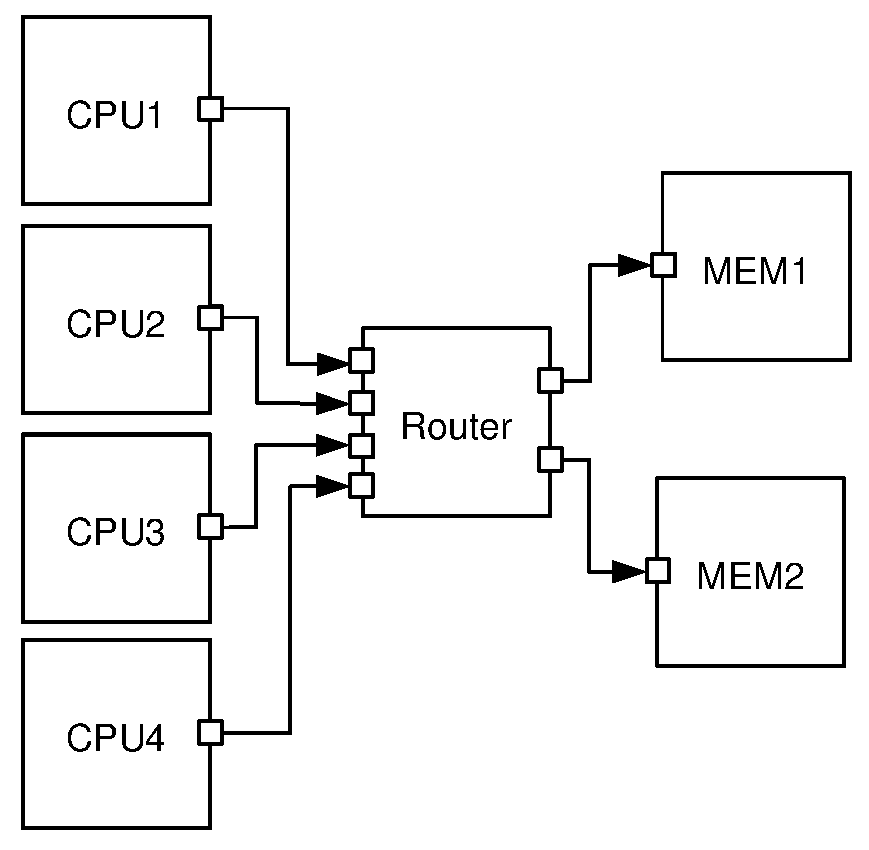
\includegraphics[width=7.0cm]{tlm/n_to_m.pdf}
    \caption{\label{fig:n_to_n} M-initiators~x~N-targets.}
  \end{center}
\end{figure}

This example shows how a module can perform contention over the
request. For that purpose a new module is added: the \texttt{router}
module which connects the processors to multiple memories, see
Figure~\ref{fig:n_to_n}. For a simple untimed implementation of the
\texttt{router} module see Figure~\ref{fig:ttlm_router}. This
implementation does not make any contention over the incomming
requests, neither over responses. This example is going to show how to
implement contention over the incomming requests, later
Section~\ref{subsec:example_response_contention} will show how to
implement contention over the responses.

The \texttt{router} module implements a round robin scheduling
algorithm to give access to the memories, i.e., if two processors are
simulated processor 0 has access to the memories during cycles 0, 2,
4,\ldots , and processor 1 at cycles 1, 3, 5,\ldots.
Figure~\ref{fig:ttlm_router_adv} shows a possible implementation. In
this implementation, the \texttt{router} module is a hierarchical
module that associates to each input port a \texttt{MasterPortModule}
module which actually implements the contention, see {\large
  \ding{202}} on Figure~\ref{fig:ttlm_router_adv}.

\texttt{MasterPortModule} bufferizes all the incomming requests and
dispatches them in the incomming order during the time windows
associated to the port using a thread. This module implements the
\texttt{Send} method from the \texttt{TlmSendIf} interface to handle
incomming requests, see {\large \ding{202}} and {\large \ding{203}} on
Figure~\ref{fig:ttlm_router_adv}. A buffer holds incomming requests
and the \texttt{Dispatch} thread of the module dispatches them to the
right output port during the time windows of the incomming port, see
{\large \ding{204}} on Figure~\ref{fig:ttlm_router_adv}.  To execute
the \texttt{Dispatch} process at the right time windows the
\texttt{dispatch\_event} (from which the \texttt{Dispatch} process
depends) has to be carefully triggered. In this example, the
\texttt{dispatch\_event} is triggered with the right delay when a new
request is queued (note that time can be equal to zero, which means
that the event will be notified during the next delta cycle, but the
SystemC clock will not be modified), see {\large \ding{205}} on
Figure~\ref{fig:ttlm_router_adv}. In case the buffer is not empty
after dispatching the oldest request (or if the oldest request has not
been accepted) another \texttt{dispatch\_event} is triggered, to
execute the \texttt{Dispatch} thread during the next time window and
send pending requests, see {\large \ding{206}} on
Figure~\ref{fig:ttlm_router_adv}.


\subsection{Example: Response contention}
\label{subsec:example_response_contention}
Section~\ref{subsec:example_request_contention} showed how contention
can be done over incomming requests. However, in many situations
contention over the responses is also desired. This example, modifies
the previously shown \texttt{router} with requests contention to
support contention over responses. For the new implementation of the
\texttt{router} see Figure~\ref{fig:ttlm_router_adv2}.

The \hfill hierarchical \hfill \texttt{router} \hfill module \hfill contains \hfill the \hfill definition \hfill of \hfill an \hfill additional \hfill module: the \texttt{SlavePortController} module, see
{\large \ding{202}} on Figure~\ref{fig:ttlm_router_adv2}. An instance
of this module is associated to each output port, and connected to
each of the instances of \texttt{MasterPortController}.

To easily handle multiple responses it implements the
\texttt{ResponseReceived} method from the \texttt{ResponseListener}
utility class (included in the source distribution of the TLM model
presented in this document), see {\large \ding{203}} and {\large
  \ding{204}} on Figure~\ref{fig:ttlm_router_adv2}.  Conceptually, the
\texttt{ResponseListener} utility class allows to send a message
through a port with the \texttt{Send} method provided by this class,
and be notified when the response is received thanks to the
\texttt{ResponseReceived} method.

The \texttt{SlavePortController} also implements the \texttt{Send}
method from the \texttt{TlmSendIf} interface to handle requests
comming from the \texttt{MasterPortController} modules, see {\large
  \ding{203}} and {\large \ding{205}} on
Figure~\ref{fig:ttlm_router_adv2}. The \texttt{Send} method checks if
the request requires a response:
\begin{itemize}
\item if not it just forwards the request to the output port, see
  {\large \ding{206}} on Figure~\ref{fig:ttlm_router_adv2};
\item if a response is required then it uses the \texttt{Send} method
  provided by the \texttt{ResponseListener} class to forward send the
  request through the output port, and be notified (through the
  \texttt{ResponseReceived} method when the response is available, see
  {\large \ding{207}} on Figure~\ref{fig:ttlm_router_adv2}.
\end{itemize}

When a response to a message is received the
\texttt{SlavePortController} handles it as the
\texttt{MasterPortController}, that is, it puts the message in a
buffer and dispatches it with the \texttt{Dispatch} thread during the
time windows given to the port, see {\large \ding{208}} on
Figure~\ref{fig:ttlm_router_adv2}.

\begin{figure}[p]
  \begin{center}
    \input{tlm/ttlm_router_adv}
    \caption{\label{fig:ttlm_router_adv} Example of TTLM router module
      with requests contention.}
  \end{center}
\end{figure}

\begin{figure}[p]
  \begin{center}
    \input{tlm/ttlm_router_adv2}
    \caption{\label{fig:ttlm_router_adv2} Example of TTLM router
      module with requests and responses contention.}
  \end{center}
\end{figure}


\chapter{Services}
\label{services}
Designing a new emulator, and particularly for a research purpose, means implementing an instruction set emulator but also involves several software components not directly related to pure instruction set execution.
The most obvious needed software components are memories, debuggers, loaders, but components such as chipsets and peripherals are still mandatory to enable running real unmodified applications.
Abstracting the underlying host hardware is also something useful to emulators.
Making all these components running together requires programming interfaces as much standard as possible.

Usually the programmer faces to the problems of sharing source codes among several emulators, reusing existing source codes, and building a fully functional emulator from all these heterogeneous pieces of source codes.
Most of the time, the software components are strongly dependent for each other: components are statically linked together through explicit function calls and adhoc interfaces.
Replacing these adhoc interfaces with C++ pure interfaces (C++ classes with only unimplemented virtual methods, see your C++ manual for more details) and linking the components through pointers is a step toward avoiding such strong dependencies between the components. But still finding a standard manner to initialize those pointers is necessary. This can be done either by directly writting in those pointers or calling special functions to do the job.

Another problem with heterogeneous software components is the manner to instantiate and parameterize those components in a standard way, so that it is easier for the component's user to use a new component.
Usually, parameterizing a component means passing arguments to an initialization function or a class constructor. It implies that the programmers agree on using only one of these two solutions or both.
Still the programmers must know the setup order of these components: it is an error prone process because determining a correct order from the components documentation will likely fail the first times.

% problems:\\
% - C++ class code sharing/reuse/composition\\
% - direct call problem\\
% - parameterization problem\\
% - setup problem: dependencies, which setup order ?\\
% \\

In this section, we propose a standard way to share, reuse, link, parameterize and setup these software components.
C++ object oriented programming and pure C++ interfaces enable sharing and reuse.
Some special pointers (classes \texttt{ServiceImport} and \texttt{ServiceExport}) linking the software components (classes \texttt{Service} and \texttt{Client}) together with some base software component classes have been introduced, thus enabling easier component composition and connection.
The parameterization have been standardized (class \texttt{Parameter}) and the framework (class \texttt{ServiceManager}) uses the call graph to provide the user with an automatic setup order.

Section~\ref{services_library} documents the available services in the library. Section~\ref{building_a_service_graph} presents how to use services, link clients and services, and setup each components. Section~\ref{designing_clients_and_services} not only presents how to design a service, either a totally new service, or an assembly of existing services, but also how to design a client invoking a service.

% solution:\\
% sharing/reuse -> classes, abstract interfaces\\
% composition -> service, client, import/export, call/use graph (connections)\\
% parameterization -> generic parameters\\
% setup problem -> call/use graph enables automatic setup order\\

\section{Service Interfaces}
\label{service_interfaces}

This section will be completed with a comprehensive documentation of the service interfaces.

\section{Services library}
\label{services_library}

The service library currently contains the following services:
\begin{itemize}
	\item Loaders: ELF loaders, PowerMac Linux Kernel Loader, PowerMac BootX emulator, S19 Loader
	\item Debug Stuff: Inline Debugger, GDB Server, Symbol Table
	\item Host hardware abstraction layer: "Simple DirectMedia Layer" wrapper (SDL)
	\item Operating System Application Binary Interface Translation (OS ABI): LinuxOS (ARM/PowerPC Linux system call translator)
	\item Host Time abstraction layer: host\_time
	\item Simulated Time abstraction layer: sc\_time
	\item Power Estimation: Cache/SRAM Power estimator based on CACTI analytical power/layout estimation tool
\end{itemize}

% \newpage
% \begin{center}
% 	\begin{tabular}{|p{7.5cm}|p{7.5cm}|}
% 		\hline
% 		\multicolumn{2}{|l|}{\textbf{\Large Service Sample}}\\
% 		\hline
% 		\multicolumn{1}{|p{7.5cm}}{\textbf{Class Name:} \newline \texttt{sample::sample::sample}\newline$\hookrightarrow$\texttt{::sample}} & \multicolumn{1}{p{7.5cm}|}{\textbf{Header:} \newline \texttt{sample/sample/sample}\newline$\hookrightarrow$\texttt{/sample.hh}}\\
% 		\multicolumn{2}{|l|}{}\\
% 		\multicolumn{2}{|p{15cm}|}{\textbf{Description:} \newline Sample.}\\
% 		\hline
% 		\hline
% 		\multicolumn{2}{|c|}{\textbf{\large Template Parameters}}\\
% 		\hline
% 		\multicolumn{1}{|p{7.5cm}}{\textbf{Name:} \texttt{sample}} & \multicolumn{1}{p{7.5cm}|}{\textbf{Type:} \texttt{sample}}\\
% 		\multicolumn{2}{|p{15cm}|}{\textbf{Default value:} \texttt{sample}}\\
% 		\multicolumn{2}{|l|}{}\\
% 		\multicolumn{2}{|p{15cm}|}{\textbf{Description:} \newline Sample.}\\
% 		\hline
% 		\hline
% 		\multicolumn{2}{|c|}{\textbf{\large Run-Time Parameters}}\\
% 		\hline
% 		\multicolumn{1}{|p{7.5cm}}{\textbf{Name:} \texttt{sample}} & \multicolumn{1}{p{7.5cm}|}{\textbf{Type:} \texttt{sample}}\\
% 		\multicolumn{2}{|p{15cm}|}{\textbf{Default value:} \texttt{sample}}\\
% 		\multicolumn{2}{|l|}{}\\
% 		\multicolumn{2}{|p{15cm}|}{\textbf{Description:} \newline Sample.}\\
% 		\hline
% 		\hline
% 		\multicolumn{2}{|c|}{\textbf{\large Service Exports}}\\
% 		\hline
% 		\multicolumn{1}{|p{7.5cm}}{\textbf{Name:} \texttt{sample}} & \multicolumn{1}{p{7.5cm}|}{\textbf{Interface:} \newline \texttt{sample} \newline$\hookrightarrow$\texttt{sample}}\\
% 		\multicolumn{2}{|l|}{}\\
% 		\multicolumn{2}{|p{15cm}|}{\textbf{Description:} \newline Sample.}\\
% 		\hline
% 		\hline
% 		\multicolumn{2}{|c|}{\textbf{\large Service Imports}}\\
% 		\hline
% 		\multicolumn{1}{|p{7.5cm}}{\textbf{Name:} \texttt{sample} \newline \textbf{Mandatory connected:} yes/no} & \multicolumn{1}{p{7.5cm}|}{\textbf{Interface:} \newline \texttt{sample::sample::sample} \newline$\hookrightarrow$\texttt{::sample}}\\
% 		\multicolumn{2}{|l|}{}\\
% 		\multicolumn{2}{|p{15cm}|}{\textbf{Description:} \newline Sample.}\\
% 		\hline
% 	\end{tabular}
% \end{center}

\subsection{Loaders}

\newpage
\begin{center}
	\begin{tabular}{|p{7.5cm}|p{7.5cm}|}
		\hline
		\multicolumn{2}{|l|}{\textbf{\Large Service ELF Loader}}\\
		\hline
		\multicolumn{1}{|p{7.5cm}}{\textbf{Class Name:} \newline \texttt{unisim::service::loader::elf\_loader}\newline$\hookrightarrow$\texttt{::ElfLoaderImpl}} & \multicolumn{1}{p{7.5cm}|}{\textbf{Header:} \newline \texttt{unisim/service/loader/elf\_loader}\newline$\hookrightarrow$\texttt{/elf\_loader.hh}}\\
		\multicolumn{2}{|l|}{}\\
		\multicolumn{2}{|p{15cm}|}{\textbf{Description:} \newline The ELF loader service allows to load a binary program into a memory and fill a symbol table.
		The loader also provides information about the loaded file such as the code and data locations (base address and size). The ELF loader loads the program during setup. \texttt{Elf32Loader} and \texttt{Elf64Loader} are two specialized versions of class \texttt{ElfLoaderImpl<>} which the user should use whenever possible.}\\
		\hline
		\hline
		\multicolumn{2}{|l|}{\textbf{Template Parameters}}\\
		\hline
		\multicolumn{1}{|p{7.5cm}}{\textbf{Name:} \texttt{MEMORY\_ADDR}} & \multicolumn{1}{p{7.5cm}|}{\textbf{Type:} \texttt{class}}\\
		\multicolumn{2}{|p{15cm}|}{\textbf{Default value:} none}\\
		\multicolumn{2}{|l|}{}\\
		\multicolumn{2}{|p{15cm}|}{\textbf{Description:} \newline This is the C++ type of a memory address (e.g. uint32\_t or uint64\_t).}\\
		\hline
		\multicolumn{1}{|p{7.5cm}}{\textbf{Name:} \texttt{ElfClass}} & \multicolumn{1}{p{7.5cm}|}{\textbf{Type:} \texttt{unsigned int}}\\
		\multicolumn{2}{|p{15cm}|}{\textbf{Default value:} none}\\
		\multicolumn{2}{|l|}{}\\
		\multicolumn{2}{|p{15cm}|}{\textbf{Description:} \newline class of machine (either \texttt{ELFCLASS32} or \texttt{ELFCLASS64}).}\\
		\hline
		\multicolumn{1}{|p{7.5cm}}{\textbf{Name:} \texttt{Elf\_Ehdr}} & \multicolumn{1}{p{7.5cm}|}{\textbf{Type:} \texttt{class}}\\
		\multicolumn{2}{|p{15cm}|}{\textbf{Default value:} none}\\
		\multicolumn{2}{|l|}{}\\
		\multicolumn{2}{|p{15cm}|}{\textbf{Description:} \newline ELF Header structure (either Elf32\_Ehdr or Elf64\_Ehdr).}\\
		\hline
		\multicolumn{1}{|p{7.5cm}}{\textbf{Name:} \texttt{Elf\_Phdr}} & \multicolumn{1}{p{7.5cm}|}{\textbf{Type:} \texttt{class}}\\
		\multicolumn{2}{|p{15cm}|}{\textbf{Default value:} none}\\
		\multicolumn{2}{|l|}{}\\
		\multicolumn{2}{|p{15cm}|}{\textbf{Description:} \newline ELF Program Header structure (either Elf32\_Phdr or Elf64\_Phdr).}\\
		\hline
		\multicolumn{1}{|p{7.5cm}}{\textbf{Name:} \texttt{Elf\_Shdr}} & \multicolumn{1}{p{7.5cm}|}{\textbf{Type:} \texttt{class}}\\
		\multicolumn{2}{|p{15cm}|}{\textbf{Default value:} none}\\
		\multicolumn{2}{|l|}{}\\
		\multicolumn{2}{|p{15cm}|}{\textbf{Description:} \newline ELF Section Header structure (either \texttt{Elf32\_Shdr} or \texttt{Elf64\_Shdr}).}\\
		\hline
		\multicolumn{1}{|p{7.5cm}}{\textbf{Name:} \texttt{Elf\_Sym}} & \multicolumn{1}{p{7.5cm}|}{\textbf{Type:} \texttt{class}}\\
		\multicolumn{2}{|p{15cm}|}{\textbf{Default value:} none}\\
		\multicolumn{2}{|l|}{}\\
		\multicolumn{2}{|p{15cm}|}{\textbf{Description:} \newline ELF Symbol structure (either \texttt{Elf32\_Sym} or \texttt{Elf64\_Sym}).}\\
		\hline
	\end{tabular}
\end{center}

\begin{center}
	\begin{tabular}{|p{7.5cm}|p{7.5cm}|}
		\hline
		\multicolumn{2}{|c|}{\textbf{\large Run-Time Parameters}}\\
		\hline
		\multicolumn{1}{|p{7.5cm}}{\textbf{Name:} \texttt{filename}} & \multicolumn{1}{p{7.5cm}|}{\textbf{Type:} \texttt{string}}\\
		\multicolumn{2}{|p{15cm}|}{\textbf{Default value:} empty string}\\
		\multicolumn{2}{|l|}{}\\
		\multicolumn{2}{|p{15cm}|}{\textbf{Description:} \newline The ELF file name to load into the connected memory.}\\
		\hline
		\multicolumn{1}{|p{7.5cm}}{\textbf{Name:} \texttt{base-addr}} & \multicolumn{1}{p{7.5cm}|}{\textbf{Type:} \texttt{MEMORY\_ADDR}}\\
		\multicolumn{2}{|p{15cm}|}{\textbf{Default value:} \texttt{0}}\\
		\multicolumn{2}{|l|}{}\\
		\multicolumn{2}{|p{15cm}|}{\textbf{Description:} \newline If this parameter is non-zero, force the ELF Loader to load the unique program segment at this base address.}\\
		\hline
		\multicolumn{1}{|p{7.5cm}}{\textbf{Name:} \texttt{force-use-virtual-address}} & \multicolumn{1}{p{7.5cm}|}{\textbf{Type:} \texttt{bool}}\\
		\multicolumn{2}{|p{15cm}|}{\textbf{Default value:} \texttt{false}}\\
		\multicolumn{2}{|l|}{}\\
		\multicolumn{2}{|p{15cm}|}{\textbf{Description:} \newline If true, this parameter forces the ELF loader to use the segment virtual address instead of the segment physical address when loading the segments into memory.}\\
		\hline
		\hline
		\multicolumn{2}{|c|}{\textbf{\large Service Exports}}\\
		\hline
		\multicolumn{1}{|p{7.5cm}}{\textbf{Name:} \texttt{logger\_export}} & \multicolumn{1}{p{7.5cm}|}{\textbf{Interface:} \newline \texttt{unisim::service::interfaces::} \newline$\hookrightarrow$\texttt{Loader<MEMORY\_ADDR>}}\\
		\multicolumn{2}{|l|}{}\\
		\multicolumn{2}{|p{15cm}|}{\textbf{Description:} \newline The ELF loader provides information about the code and data location through this export.}\\
		\hline
		\hline
		\multicolumn{2}{|c|}{\textbf{\large Service Imports}}\\
		\hline
		\multicolumn{1}{|p{7.5cm}}{\textbf{Name:} \texttt{memory\_import}} & \multicolumn{1}{p{7.5cm}|}{\textbf{Interface:} \newline \texttt{unisim::service::interfaces::} \newline$\hookrightarrow$\texttt{Memory<MEMORY\_ADDR>}}\\
		\multicolumn{2}{|p{15cm}|}{\textbf{Mandatory connected:} no}\\
		\multicolumn{2}{|l|}{}\\
		\multicolumn{2}{|p{15cm}|}{\textbf{Description:} \newline The ELF loader accesses to the memory through this import.}\\
		\hline
		\multicolumn{1}{|p{7.5cm}}{\textbf{Name:} \texttt{symbol\_table\_build\_import}} & \multicolumn{1}{p{7.5cm}|}{\textbf{Interface:} \newline \texttt{unisim::service::interfaces::} \newline$\hookrightarrow$\texttt{SymbolTableBuild<MEMORY\_ADDR>}}\\
		\multicolumn{2}{|p{15cm}|}{\textbf{Mandatory connected:} no}\\
		\multicolumn{2}{|l|}{}\\
		\multicolumn{2}{|p{15cm}|}{\textbf{Description:} \newline The ELF loader fills the symbol table using this import.}\\
		\hline
	\end{tabular}
\end{center}

\newpage
\begin{center}
	\begin{tabular}{|p{7.5cm}|p{7.5cm}|}
		\hline
		\multicolumn{2}{|l|}{\textbf{\Large Service ELF32 Loader}}\\
		\hline
		\multicolumn{1}{|p{7.5cm}}{\textbf{Class Name:} \newline \texttt{unisim::service::loader::elf\_loader}\newline$\hookrightarrow$\texttt{::Elf32Loader}} & \multicolumn{1}{p{7.5cm}|}{\textbf{Header:} \newline \texttt{unisim/service/loader/elf\_loader}\newline$\hookrightarrow$\texttt{/elf\_loader.hh}}\\
		\multicolumn{2}{|l|}{}\\
		\multicolumn{2}{|p{15cm}|}{\textbf{Description:} \newline The ELF32 loader service allows to load an ELF32 binary program into a memory and fill a symbol table. The loader also provides information about the loaded file such as the code and data locations (base address and size). The ELF loader loads the program during setup.}\\
		\hline
		\hline
		\multicolumn{2}{|c|}{\textbf{\large Run-Time Parameters}}\\
		\hline
		\multicolumn{1}{|p{7.5cm}}{\textbf{Name:} \texttt{filename}} & \multicolumn{1}{p{7.5cm}|}{\textbf{Type:} \texttt{string}}\\
		\multicolumn{2}{|p{15cm}|}{\textbf{Default value:} empty string}\\
		\multicolumn{2}{|l|}{}\\
		\multicolumn{2}{|p{15cm}|}{\textbf{Description:} \newline The ELF file name to load into the connected memory.}\\
		\hline
		\multicolumn{1}{|p{7.5cm}}{\textbf{Name:} \texttt{base-addr}} & \multicolumn{1}{p{7.5cm}|}{\textbf{Type:} \texttt{uint32\_t}}\\
		\multicolumn{2}{|p{15cm}|}{\textbf{Default value:} \texttt{0}}\\
		\multicolumn{2}{|l|}{}\\
		\multicolumn{2}{|p{15cm}|}{\textbf{Description:} \newline If this parameter is non-zero, force the ELF Loader to load the unique program segment at this base address.}\\
		\hline
		\multicolumn{1}{|p{7.5cm}}{\textbf{Name:} \texttt{force-use-virtual-address}} & \multicolumn{1}{p{7.5cm}|}{\textbf{Type:} \texttt{bool}}\\
		\multicolumn{2}{|p{15cm}|}{\textbf{Default value:} \texttt{false}}\\
		\multicolumn{2}{|l|}{}\\
		\multicolumn{2}{|p{15cm}|}{\textbf{Description:} \newline If true, this parameter forces the ELF loader to use the segment virtual address instead of the segment physical address when loading the segments into memory.}\\
		\hline
		\hline
		\multicolumn{2}{|c|}{\textbf{\large Service Exports}}\\
		\hline
		\multicolumn{1}{|p{7.5cm}}{\textbf{Name:} \texttt{logger\_export}} & \multicolumn{1}{p{7.5cm}|}{\textbf{Interface:} \newline \texttt{unisim::service::interfaces::} \newline$\hookrightarrow$\texttt{Loader<uint32\_t>}}\\
		\multicolumn{2}{|l|}{}\\
		\multicolumn{2}{|p{15cm}|}{\textbf{Description:} \newline The ELF loader provides information about the code and data location through this export.}\\
		\hline
		\hline
		\multicolumn{2}{|c|}{\textbf{\large Service Imports}}\\
		\hline
		\multicolumn{1}{|p{7.5cm}}{\textbf{Name:} \texttt{memory\_import} \newline \textbf{Mandatory connected:} no} & \multicolumn{1}{p{7.5cm}|}{\textbf{Interface:} \newline \texttt{unisim::service::interfaces::} \newline$\hookrightarrow$\texttt{Memory<uint32\_t>}}\\
		\multicolumn{2}{|l|}{}\\
		\multicolumn{2}{|p{15cm}|}{\textbf{Description:} \newline The ELF loader accesses to the memory through this import.}\\
		\hline
		\multicolumn{1}{|p{7.5cm}}{\textbf{Name:} \texttt{symbol\_table\_build\_import} \newline \textbf{Mandatory connected:} no} & \multicolumn{1}{p{7.5cm}|}{\textbf{Interface:} \newline \texttt{unisim::service::interfaces::} \newline$\hookrightarrow$\texttt{SymbolTableBuild<uint32\_t>}}\\
		\multicolumn{2}{|l|}{}\\
		\multicolumn{2}{|p{15cm}|}{\textbf{Description:} \newline The ELF loader fills the symbol table using this import.}\\
		\hline
	\end{tabular}
\end{center}

\newpage
\begin{center}
	\begin{tabular}{|p{7.5cm}|p{7.5cm}|}
		\hline
		\multicolumn{2}{|l|}{\textbf{\Large Service ELF64 Loader}}\\
		\hline
		\multicolumn{1}{|p{7.5cm}}{\textbf{Class Name:} \newline \texttt{unisim::service::loader::elf\_loader}\newline$\hookrightarrow$\texttt{::Elf32Loader}} & \multicolumn{1}{p{7.5cm}|}{\textbf{Header:} \newline \texttt{unisim/service/loader/elf\_loader}\newline$\hookrightarrow$\texttt{/elf\_loader.hh}}\\
		\multicolumn{2}{|l|}{}\\
		\multicolumn{2}{|p{15cm}|}{\textbf{Description:} \newline The ELF32 loader service allows to load an ELF64 binary program into a memory and fill a symbol table. The loader also provides information about the loaded file such as the code and data locations (base address and size). The ELF loader loads the program during setup.}\\
		\hline
		\hline
		\multicolumn{2}{|c|}{\textbf{\large Run-Time Parameters}}\\
		\hline
		\multicolumn{1}{|p{7.5cm}}{\textbf{Name:} \texttt{filename}} & \multicolumn{1}{p{7.5cm}|}{\textbf{Type:} \texttt{string}}\\
		\multicolumn{2}{|p{15cm}|}{\textbf{Default value:} empty string}\\
		\multicolumn{2}{|l|}{}\\
		\multicolumn{2}{|p{15cm}|}{\textbf{Description:} \newline The ELF file name to load into the connected memory.}\\
		\hline
		\multicolumn{1}{|p{7.5cm}}{\textbf{Name:} \texttt{base-addr}} & \multicolumn{1}{p{7.5cm}|}{\textbf{Type:} \texttt{uint64\_t}}\\
		\multicolumn{2}{|p{15cm}|}{\textbf{Default value:} \texttt{0}}\\
		\multicolumn{2}{|l|}{}\\
		\multicolumn{2}{|p{15cm}|}{\textbf{Description:} \newline If this parameter is non-zero, force the ELF Loader to load the unique program segment at this base address.}\\
		\hline
		\multicolumn{1}{|p{7.5cm}}{\textbf{Name:} \texttt{force-use-virtual-address}} & \multicolumn{1}{p{7.5cm}|}{\textbf{Type:} \texttt{bool}}\\
		\multicolumn{2}{|p{15cm}|}{\textbf{Default value:} \texttt{false}}\\
		\multicolumn{2}{|l|}{}\\
		\multicolumn{2}{|p{15cm}|}{\textbf{Description:} \newline If true, this parameter forces the ELF loader to use the segment virtual address instead of the segment physical address when loading the segments into memory.}\\
		\hline
		\hline
		\multicolumn{2}{|c|}{\textbf{\large Service Exports}}\\
		\hline
		\multicolumn{1}{|p{7.5cm}}{\textbf{Name:} \texttt{logger\_export}} & \multicolumn{1}{p{7.5cm}|}{\textbf{Interface:} \newline \texttt{unisim::service::interfaces::} \newline$\hookrightarrow$\texttt{Loader<uint64\_t>}}\\
		\multicolumn{2}{|l|}{}\\
		\multicolumn{2}{|p{15cm}|}{\textbf{Description:} \newline The ELF loader provides information about the code and data location through this export.}\\
		\hline
		\hline
		\multicolumn{2}{|c|}{\textbf{\large Service Imports}}\\
		\hline
		\multicolumn{1}{|p{7.5cm}}{\textbf{Name:} \texttt{memory\_import} \newline \textbf{Mandatory connected:} no} & \multicolumn{1}{p{7.5cm}|}{\textbf{Interface:} \newline \texttt{unisim::service::interfaces::} \newline$\hookrightarrow$\texttt{Memory<uint64\_t>}}\\
		\multicolumn{2}{|l|}{}\\
		\multicolumn{2}{|p{15cm}|}{\textbf{Description:} \newline The ELF loader accesses to the memory through this import.}\\
		\hline
		\multicolumn{1}{|p{7.5cm}}{\textbf{Name:} \texttt{symbol\_table\_build\_import} \newline \textbf{Mandatory connected:} no} & \multicolumn{1}{p{7.5cm}|}{\textbf{Interface:} \newline \texttt{unisim::service::interfaces::} \newline$\hookrightarrow$\texttt{SymbolTableBuild<uint64\_t>}}\\
		\multicolumn{2}{|l|}{}\\
		\multicolumn{2}{|p{15cm}|}{\textbf{Description:} \newline The ELF loader fills the symbol table using this import.}\\
		\hline
	\end{tabular}
\end{center}

\newpage
\begin{center}
	\begin{tabular}{|p{7.5cm}|p{7.5cm}|}
		\hline
		\multicolumn{2}{|l|}{\textbf{\Large Service PowerMac Linux Kernel Loader}}\\
		\hline
		\multicolumn{1}{|p{7.5cm}}{\textbf{Class Name:} \newline \texttt{sample::sample::sample}\newline$\hookrightarrow$\texttt{::sample}} & \multicolumn{1}{p{7.5cm}|}{\textbf{Header:} \newline \texttt{sample/sample/sample}\newline$\hookrightarrow$\texttt{/sample.hh}}\\
		\multicolumn{2}{|l|}{}\\
		\multicolumn{2}{|p{15cm}|}{\textbf{Description:} \newline Sample.}\\
		\hline
		\hline
		\multicolumn{2}{|c|}{\textbf{\large Template Parameters}}\\
		\hline
		\multicolumn{1}{|p{7.5cm}}{\textbf{Name:} \texttt{sample}} & \multicolumn{1}{p{7.5cm}|}{\textbf{Type:} \texttt{sample}}\\
		\multicolumn{2}{|p{15cm}|}{\textbf{Default value:} \texttt{sample}}\\
		\multicolumn{2}{|l|}{}\\
		\multicolumn{2}{|p{15cm}|}{\textbf{Description:} \newline Sample.}\\
		\hline
		\hline
		\multicolumn{2}{|c|}{\textbf{\large Run-Time Parameters}}\\
		\hline
		\multicolumn{1}{|p{7.5cm}}{\textbf{Name:} \texttt{sample}} & \multicolumn{1}{p{7.5cm}|}{\textbf{Type:} \texttt{sample}}\\
		\multicolumn{2}{|p{15cm}|}{\textbf{Default value:} \texttt{sample}}\\
		\multicolumn{2}{|l|}{}\\
		\multicolumn{2}{|p{15cm}|}{\textbf{Description:} \newline Sample.}\\
		\hline
		\hline
		\multicolumn{2}{|c|}{\textbf{\large Service Exports}}\\
		\hline
		\multicolumn{1}{|p{7.5cm}}{\textbf{Name:} \texttt{sample}} & \multicolumn{1}{p{7.5cm}|}{\textbf{Interface:} \newline \texttt{sample} \newline$\hookrightarrow$\texttt{sample}}\\
		\multicolumn{2}{|l|}{}\\
		\multicolumn{2}{|p{15cm}|}{\textbf{Description:} \newline Sample.}\\
		\hline
		\hline
		\multicolumn{2}{|c|}{\textbf{\large Service Imports}}\\
		\hline
		\multicolumn{1}{|p{7.5cm}}{\textbf{Name:} \texttt{sample} \newline \textbf{Mandatory connected:} yes/no} & \multicolumn{1}{p{7.5cm}|}{\textbf{Interface:} \newline \texttt{sample::sample::sample} \newline$\hookrightarrow$\texttt{::sample}}\\
		\multicolumn{2}{|l|}{}\\
		\multicolumn{2}{|p{15cm}|}{\textbf{Description:} \newline Sample.}\\
		\hline
	\end{tabular}
\end{center}

\newpage
\begin{center}
	\begin{tabular}{|p{7.5cm}|p{7.5cm}|}
		\hline
		\multicolumn{2}{|l|}{\textbf{\Large Service PowerMac BootX Loader}}\\
		\hline
		\multicolumn{1}{|p{7.5cm}}{\textbf{Class Name:} \newline \texttt{sample::sample::sample}\newline$\hookrightarrow$\texttt{::sample}} & \multicolumn{1}{p{7.5cm}|}{\textbf{Header:} \newline \texttt{sample/sample/sample}\newline$\hookrightarrow$\texttt{/sample.hh}}\\
		\multicolumn{2}{|l|}{}\\
		\multicolumn{2}{|p{15cm}|}{\textbf{Description:} \newline Sample.}\\
		\hline
		\hline
		\multicolumn{2}{|c|}{\textbf{\large Template Parameters}}\\
		\hline
		\multicolumn{1}{|p{7.5cm}}{\textbf{Name:} \texttt{sample}} & \multicolumn{1}{p{7.5cm}|}{\textbf{Type:} \texttt{sample}}\\
		\multicolumn{2}{|p{15cm}|}{\textbf{Default value:} \texttt{sample}}\\
		\multicolumn{2}{|l|}{}\\
		\multicolumn{2}{|p{15cm}|}{\textbf{Description:} \newline Sample.}\\
		\hline
		\hline
		\multicolumn{2}{|c|}{\textbf{\large Run-Time Parameters}}\\
		\hline
		\multicolumn{1}{|p{7.5cm}}{\textbf{Name:} \texttt{sample}} & \multicolumn{1}{p{7.5cm}|}{\textbf{Type:} \texttt{sample}}\\
		\multicolumn{2}{|p{15cm}|}{\textbf{Default value:} \texttt{sample}}\\
		\multicolumn{2}{|l|}{}\\
		\multicolumn{2}{|p{15cm}|}{\textbf{Description:} \newline Sample.}\\
		\hline
		\hline
		\multicolumn{2}{|c|}{\textbf{\large Service Exports}}\\
		\hline
		\multicolumn{1}{|p{7.5cm}}{\textbf{Name:} \texttt{sample}} & \multicolumn{1}{p{7.5cm}|}{\textbf{Interface:} \newline \texttt{sample} \newline$\hookrightarrow$\texttt{sample}}\\
		\multicolumn{2}{|l|}{}\\
		\multicolumn{2}{|p{15cm}|}{\textbf{Description:} \newline Sample.}\\
		\hline
		\hline
		\multicolumn{2}{|c|}{\textbf{\large Service Imports}}\\
		\hline
		\multicolumn{1}{|p{7.5cm}}{\textbf{Name:} \texttt{sample} \newline \textbf{Mandatory connected:} yes/no} & \multicolumn{1}{p{7.5cm}|}{\textbf{Interface:} \newline \texttt{sample::sample::sample} \newline$\hookrightarrow$\texttt{::sample}}\\
		\multicolumn{2}{|l|}{}\\
		\multicolumn{2}{|p{15cm}|}{\textbf{Description:} \newline Sample.}\\
		\hline
	\end{tabular}
\end{center}

\newpage
\begin{center}
	\begin{tabular}{|p{7.5cm}|p{7.5cm}|}
		\hline
		\multicolumn{2}{|l|}{\textbf{\Large Service S19 Loader}}\\
		\hline
		\multicolumn{1}{|p{7.5cm}}{\textbf{Class Name:} \newline \texttt{sample::sample::sample}\newline$\hookrightarrow$\texttt{::sample}} & \multicolumn{1}{p{7.5cm}|}{\textbf{Header:} \newline \texttt{sample/sample/sample}\newline$\hookrightarrow$\texttt{/sample.hh}}\\
		\multicolumn{2}{|l|}{}\\
		\multicolumn{2}{|p{15cm}|}{\textbf{Description:} \newline Sample.}\\
		\hline
		\hline
		\multicolumn{2}{|c|}{\textbf{\large Template Parameters}}\\
		\hline
		\multicolumn{1}{|p{7.5cm}}{\textbf{Name:} \texttt{sample}} & \multicolumn{1}{p{7.5cm}|}{\textbf{Type:} \texttt{sample}}\\
		\multicolumn{2}{|p{15cm}|}{\textbf{Default value:} \texttt{sample}}\\
		\multicolumn{2}{|l|}{}\\
		\multicolumn{2}{|p{15cm}|}{\textbf{Description:} \newline Sample.}\\
		\hline
		\hline
		\multicolumn{2}{|c|}{\textbf{\large Run-Time Parameters}}\\
		\hline
		\multicolumn{1}{|p{7.5cm}}{\textbf{Name:} \texttt{sample}} & \multicolumn{1}{p{7.5cm}|}{\textbf{Type:} \texttt{sample}}\\
		\multicolumn{2}{|p{15cm}|}{\textbf{Default value:} \texttt{sample}}\\
		\multicolumn{2}{|l|}{}\\
		\multicolumn{2}{|p{15cm}|}{\textbf{Description:} \newline Sample.}\\
		\hline
		\hline
		\multicolumn{2}{|c|}{\textbf{\large Service Exports}}\\
		\hline
		\multicolumn{1}{|p{7.5cm}}{\textbf{Name:} \texttt{sample}} & \multicolumn{1}{p{7.5cm}|}{\textbf{Interface:} \newline \texttt{sample} \newline$\hookrightarrow$\texttt{sample}}\\
		\multicolumn{2}{|l|}{}\\
		\multicolumn{2}{|p{15cm}|}{\textbf{Description:} \newline Sample.}\\
		\hline
		\hline
		\multicolumn{2}{|c|}{\textbf{\large Service Imports}}\\
		\hline
		\multicolumn{1}{|p{7.5cm}}{\textbf{Name:} \texttt{sample} \newline \textbf{Mandatory connected:} yes/no} & \multicolumn{1}{p{7.5cm}|}{\textbf{Interface:} \newline \texttt{sample::sample::sample} \newline$\hookrightarrow$\texttt{::sample}}\\
		\multicolumn{2}{|l|}{}\\
		\multicolumn{2}{|p{15cm}|}{\textbf{Description:} \newline Sample.}\\
		\hline
	\end{tabular}
\end{center}

\newpage
\begin{center}
	\begin{tabular}{|p{7.5cm}|p{7.5cm}|}
		\hline
		\multicolumn{2}{|l|}{\textbf{\Large Service COFF Loader}}\\
		\hline
		\multicolumn{1}{|p{7.5cm}}{\textbf{Class Name:} \newline \texttt{unisim::service::loader::coff\_loader}\newline$\hookrightarrow$\texttt{::CoffLoader}} & \multicolumn{1}{p{7.5cm}|}{\textbf{Header:} \newline \texttt{unisim/service/loader/coff\_loader}\newline$\hookrightarrow$\texttt{/coff\_loader.hh}}\\
		\multicolumn{2}{|l|}{}\\
		\multicolumn{2}{|p{15cm}|}{\textbf{Description:} \newline The COFF loader service allows to load a COFF binary program into a memory and fill a symbol table. The loader also provides information about the loaded file such as the code and data locations (base address and size). The COFF loader loads the program during setup.}\\
		\hline
		\hline
		\multicolumn{2}{|c|}{\textbf{\large Template Parameters}}\\
		\hline
		\multicolumn{1}{|p{7.5cm}}{\textbf{Name:} \texttt{MEMORY\_ADDR}} & \multicolumn{1}{p{7.5cm}|}{\textbf{Type:} \texttt{class}}\\
		\multicolumn{2}{|p{15cm}|}{\textbf{Default value:} \texttt{none}}\\
		\multicolumn{2}{|l|}{}\\
		\multicolumn{2}{|p{15cm}|}{\textbf{Description:} \newline This is the C++ type of a memory address (e.g. \texttt{uint32\_t} or \texttt{uint64\_t}).}\\
		\hline
		\hline
		\multicolumn{2}{|c|}{\textbf{\large Run-Time Parameters}}\\
		\hline
		\multicolumn{1}{|p{7.5cm}}{\textbf{Name:} \texttt{filename}} & \multicolumn{1}{p{7.5cm}|}{\textbf{Type:} \texttt{string}}\\
		\multicolumn{2}{|p{15cm}|}{\textbf{Default value:} empty string}\\
		\multicolumn{2}{|l|}{}\\
		\multicolumn{2}{|p{15cm}|}{\textbf{Description:} \newline The COFF file name to load into the connected memory.}\\
		\hline
		\hline
		\multicolumn{1}{|p{7.5cm}}{\textbf{Name:} \texttt{dump-headers}} & \multicolumn{1}{p{7.5cm}|}{\textbf{Type:} \texttt{boolean}}\\
		\multicolumn{2}{|p{15cm}|}{\textbf{Default value:} false}\\
		\multicolumn{2}{|l|}{}\\
		\multicolumn{2}{|p{15cm}|}{\textbf{Description:} \newline If true this parameter makes the COFF loader print the file headers on the screen (file header, section headers, symbol table \ldots) while loading the program.}\\
		\hline
		\hline
		\multicolumn{2}{|c|}{\textbf{\large Service Exports}}\\
		\hline
		\multicolumn{1}{|p{7.5cm}}{\textbf{Name:} \texttt{logger\_export}} & \multicolumn{1}{p{7.5cm}|}{\textbf{Interface:} \newline \texttt{unisim::service::interfaces::} \newline$\hookrightarrow$\texttt{Loader<MEMORY\_ADDR>}}\\
		\multicolumn{2}{|l|}{}\\
		\multicolumn{2}{|p{15cm}|}{\textbf{Description:} \newline The COFF loader provides information about the code and data location through this export.}\\
		\hline
		\multicolumn{1}{|p{7.5cm}}{\textbf{Name:} \texttt{symbol\_table\_lookup\_export}} & \multicolumn{1}{p{7.5cm}|}{\textbf{Interface:} \newline \texttt{unisim::service::interfaces::} \newline$\hookrightarrow$\texttt{SymbolTableLookup<MEMORY\_ADDR>}}\\
		\multicolumn{2}{|l|}{}\\
		\multicolumn{2}{|p{15cm}|}{\textbf{Description:} \newline The COFF loader provides symbol lookup through this export.}\\
		\hline
		\hline
		\multicolumn{2}{|c|}{\textbf{\large Service Imports}}\\
		\hline
		\multicolumn{1}{|p{7.5cm}}{\textbf{Name:} \texttt{memory\_import} \newline \textbf{Mandatory connected:} no} & \multicolumn{1}{p{7.5cm}|}{\textbf{Interface:} \newline \texttt{unisim::service::interfaces::} \newline$\hookrightarrow$\texttt{Memory<uint32\_t>}}\\
		\multicolumn{2}{|l|}{}\\
		\multicolumn{2}{|p{15cm}|}{\textbf{Description:} \newline The COFF loader accesses to the memory through this import.}\\
		\hline
	\end{tabular}
\end{center}

\subsection{Operating System Application Binary Interface (OS ABI)}

\newpage
\begin{center}
	\begin{tabular}{|p{7.5cm}|p{7.5cm}|}
		\hline
		\multicolumn{2}{|l|}{\textbf{\Large Service Linux System Call Translator: LinuxOS}}\\
		\hline
		\multicolumn{1}{|p{7.5cm}}{\textbf{Class Name:} \newline \texttt{sample::sample::sample}\newline$\hookrightarrow$\texttt{::sample}} & \multicolumn{1}{p{7.5cm}|}{\textbf{Header:} \newline \texttt{sample/sample/sample}\newline$\hookrightarrow$\texttt{/sample.hh}}\\
		\multicolumn{2}{|l|}{}\\
		\multicolumn{2}{|p{15cm}|}{\textbf{Description:} \newline Sample.}\\
		\hline
		\hline
		\multicolumn{2}{|c|}{\textbf{\large Template Parameters}}\\
		\hline
		\multicolumn{1}{|p{7.5cm}}{\textbf{Name:} \texttt{sample}} & \multicolumn{1}{p{7.5cm}|}{\textbf{Type:} \texttt{sample}}\\
		\multicolumn{2}{|p{15cm}|}{\textbf{Default value:} \texttt{sample}}\\
		\multicolumn{2}{|l|}{}\\
		\multicolumn{2}{|p{15cm}|}{\textbf{Description:} \newline Sample.}\\
		\hline
		\hline
		\multicolumn{2}{|c|}{\textbf{\large Run-Time Parameters}}\\
		\hline
		\multicolumn{1}{|p{7.5cm}}{\textbf{Name:} \texttt{sample}} & \multicolumn{1}{p{7.5cm}|}{\textbf{Type:} \texttt{sample}}\\
		\multicolumn{2}{|p{15cm}|}{\textbf{Default value:} \texttt{sample}}\\
		\multicolumn{2}{|l|}{}\\
		\multicolumn{2}{|p{15cm}|}{\textbf{Description:} \newline Sample.}\\
		\hline
		\hline
		\multicolumn{2}{|c|}{\textbf{\large Service Exports}}\\
		\hline
		\multicolumn{1}{|p{7.5cm}}{\textbf{Name:} \texttt{sample}} & \multicolumn{1}{p{7.5cm}|}{\textbf{Interface:} \newline \texttt{sample} \newline$\hookrightarrow$\texttt{sample}}\\
		\multicolumn{2}{|l|}{}\\
		\multicolumn{2}{|p{15cm}|}{\textbf{Description:} \newline Sample.}\\
		\hline
		\hline
		\multicolumn{2}{|c|}{\textbf{\large Service Imports}}\\
		\hline
		\multicolumn{1}{|p{7.5cm}}{\textbf{Name:} \texttt{sample} \newline \textbf{Mandatory connected:} yes/no} & \multicolumn{1}{p{7.5cm}|}{\textbf{Interface:} \newline \texttt{sample::sample::sample} \newline$\hookrightarrow$\texttt{::sample}}\\
		\multicolumn{2}{|l|}{}\\
		\multicolumn{2}{|p{15cm}|}{\textbf{Description:} \newline Sample.}\\
		\hline
	\end{tabular}
\end{center}

\newpage
\begin{center}
	\begin{tabular}{|p{7.5cm}|p{7.5cm}|}
		\hline
		\multicolumn{2}{|l|}{\textbf{\Large Service TI C I/O}}\\
		\hline
		\multicolumn{1}{|p{7.5cm}}{\textbf{Class Name:} \newline \texttt{unisim::service::os::ti\_c\_io}\newline$\hookrightarrow$\texttt{::TI\_C\_IO}} & \multicolumn{1}{p{7.5cm}|}{\textbf{Header:} \newline \texttt{unisim/service/os/ti\_c\_io}\newline$\hookrightarrow$\texttt{/ti\_c\_io.hh}}\\
		\multicolumn{2}{|l|}{}\\
		\multicolumn{2}{|p{15cm}|}{\textbf{Description:} \newline The TI C I/O service provides target programs with a support for low level I/O (open, read, write, close, \ldots) on the host machine.}\\
		\hline
		\hline
		\multicolumn{2}{|c|}{\textbf{\large Template Parameters}}\\
		\hline
		\multicolumn{1}{|p{7.5cm}}{\textbf{Name:} \texttt{MEMORY\_ADDR}} & \multicolumn{1}{p{7.5cm}|}{\textbf{Type:} \texttt{class}}\\
		\multicolumn{2}{|p{15cm}|}{\textbf{Default value:} \texttt{none}}\\
		\multicolumn{2}{|l|}{}\\
		\multicolumn{2}{|p{15cm}|}{\textbf{Description:} \newline This is the C++ type of a memory address (e.g. uint32\_t or uint64\_t).}\\
		\hline
		\hline
		\multicolumn{2}{|c|}{\textbf{\large Run-Time Parameters}}\\
		\hline
		\multicolumn{1}{|p{7.5cm}}{\textbf{Name:} \texttt{ti\_c\_io.enable}} & \multicolumn{1}{p{7.5cm}|}{\textbf{Type:} \texttt{bool}}\\
		\multicolumn{2}{|p{15cm}|}{\textbf{Default value:} \texttt{false}}\\
		\multicolumn{2}{|l|}{}\\
		\multicolumn{2}{|p{15cm}|}{\textbf{Description:} \newline Enable/Disable TI C I/O support.}\\
		\hline
		\multicolumn{1}{|p{7.5cm}}{\textbf{Name:} \texttt{ti-c-io.warning-as-error}} & \multicolumn{1}{p{7.5cm}|}{\textbf{Type:} \texttt{bool}}\\
		\multicolumn{2}{|p{15cm}|}{\textbf{Default value:} \texttt{false}}\\
		\multicolumn{2}{|l|}{}\\
		\multicolumn{2}{|p{15cm}|}{\textbf{Description:} \newline Whether Warnings are considered as error or not.}\\
		\hline
		\multicolumn{1}{|p{7.5cm}}{\textbf{Name:} \texttt{ti-c-io.pc-register-name}} & \multicolumn{1}{p{7.5cm}|}{\textbf{Type:} \texttt{string}}\\
		\multicolumn{2}{|p{15cm}|}{\textbf{Default value:} \texttt{"PC"}}\\
		\multicolumn{2}{|l|}{}\\
		\multicolumn{2}{|p{15cm}|}{\textbf{Description:} \newline Name of the CPU program counter register.}\\
		\hline
		\multicolumn{1}{|p{7.5cm}}{\textbf{Name:} \texttt{ti-c-io.c-io-buffer-symbol-name}} & \multicolumn{1}{p{7.5cm}|}{\textbf{Type:} \texttt{string}}\\
		\multicolumn{2}{|p{15cm}|}{\textbf{Default value:} \texttt{"\_\_CIOBUF\_"}}\\
		\multicolumn{2}{|l|}{}\\
		\multicolumn{2}{|p{15cm}|}{\textbf{Description:} \newline C I/O buffer symbol name.}\\
		\hline
		\multicolumn{1}{|p{7.5cm}}{\textbf{Name:} \texttt{ti-c-io.c-io-breakpoint-}\newline$\hookrightarrow$\texttt{symbol-name}} & \multicolumn{1}{p{7.5cm}|}{\textbf{Type:} \texttt{string}}\\
		\multicolumn{2}{|p{15cm}|}{\textbf{Default value:} \texttt{"C\$\$IO\$\$"}}\\
		\multicolumn{2}{|l|}{}\\
		\multicolumn{2}{|p{15cm}|}{\textbf{Description:} \newline C I/O breakpoint symbol name. The TI C I/O service installs an SWI instruction at this point to capture target program I/O.}\\
		\hline
		\multicolumn{1}{|p{7.5cm}}{\textbf{Name:} \texttt{ti-c-io.c-exit-breakpoint-}\newline$\hookrightarrow$\texttt{symbol-name}} & \multicolumn{1}{p{7.5cm}|}{\textbf{Type:} \texttt{string}}\\
		\multicolumn{2}{|p{15cm}|}{\textbf{Default value:} \texttt{"C\$\$EXIT"}}\\
		\multicolumn{2}{|l|}{}\\
		\multicolumn{2}{|p{15cm}|}{\textbf{Description:} \newline C EXIT breakpoint symbol name. The TI C I/O service installs an SWI instruction at this point to capture target program exit.}\\
		\hline
	\end{tabular}
\end{center}

\newpage
\begin{center}
	\begin{tabular}{|p{7.5cm}|p{7.5cm}|}
		\hline
		\multicolumn{1}{|p{7.5cm}}{\textbf{Name:} \texttt{ti-c-io.verbose-all}} & \multicolumn{1}{p{7.5cm}|}{\textbf{Type:} \texttt{bool}}\\
		\multicolumn{2}{|p{15cm}|}{\textbf{Default value:} \texttt{false}}\\
		\multicolumn{2}{|l|}{}\\
		\multicolumn{2}{|p{15cm}|}{\textbf{Description:} \newline Globally enable/disable verbosity of TI C I/O service.}\\
		\hline
		\multicolumn{1}{|p{7.5cm}}{\textbf{Name:} \texttt{ti-c-io.verbose-io}} & \multicolumn{1}{p{7.5cm}|}{\textbf{Type:} \texttt{bool}}\\
		\multicolumn{2}{|p{15cm}|}{\textbf{Default value:} \texttt{false}}\\
		\multicolumn{2}{|l|}{}\\
		\multicolumn{2}{|p{15cm}|}{\textbf{Description:} \newline Enable/disable verbosity of TI C I/O service while I/Os.}\\
		\hline
		\multicolumn{1}{|p{7.5cm}}{\textbf{Name:} \texttt{ti-c-io.verbose-setup}} & \multicolumn{1}{p{7.5cm}|}{\textbf{Type:} \texttt{bool}}\\
		\multicolumn{2}{|p{15cm}|}{\textbf{Default value:} \texttt{false}}\\
		\multicolumn{2}{|l|}{}\\
		\multicolumn{2}{|p{15cm}|}{\textbf{Description:} \newline Enable/disable verbosity of TI C I/O service while setup.}\\
		\hline
		\hline
		\multicolumn{2}{|c|}{\textbf{\large Service Exports}}\\
		\hline
		\multicolumn{1}{|p{7.5cm}}{\textbf{Name:} \texttt{ti\_c\_io\_export}} & \multicolumn{1}{p{7.5cm}|}{\textbf{Interface:} \newline \texttt{unisim::interfaces::} \newline$\hookrightarrow$\texttt{TI\_C\_IO<MEMORY\_ADDR>}}\\
		\multicolumn{2}{|l|}{}\\
		\multicolumn{2}{|p{15cm}|}{\textbf{Description:} \newline The TI C I/O provides target to host I/O translation through this service export.}\\
		\hline
		\hline
		\multicolumn{2}{|c|}{\textbf{\large Service Imports}}\\
		\hline
		\multicolumn{1}{|p{7.5cm}}{\textbf{Name:} \texttt{memory\_import}} & \multicolumn{1}{p{7.5cm}|}{\textbf{Interface:} \newline \texttt{unisim::service::interfaces::} \newline$\hookrightarrow$\texttt{Memory<MEMORY\_ADDR>}}\\
		\multicolumn{2}{|p{15cm}|}{\textbf{Mandatory connected:} no}\\
		\multicolumn{2}{|l|}{}\\
		\multicolumn{2}{|p{15cm}|}{\textbf{Description:} \newline The TI C I/O service accesses to the memory while setup through this import. While setup it installs a two SWI instructions to capture both target I/O and program exit.}\\
		\hline
		\multicolumn{1}{|p{7.5cm}}{\textbf{Name:} \texttt{memory\_injection\_import}} & \multicolumn{1}{p{7.5cm}|}{\textbf{Interface:} \newline \texttt{unisim::service::interfaces::} \newline$\hookrightarrow$\texttt{MemoryInjection<MEMORY\_ADDR>}}\\
		\multicolumn{2}{|p{15cm}|}{\textbf{Mandatory connected:} no}\\
		\multicolumn{2}{|l|}{}\\
		\multicolumn{2}{|p{15cm}|}{\textbf{Description:} \newline The TI C I/O service accesses to the memory while simulation through this import. It accesses to the I/O buffer in the target program memory and then interprete the content of this buffer to translate target program I/Os to host I/Os.}\\
		\hline
		\multicolumn{1}{|p{7.5cm}}{\textbf{Name:} \texttt{registers\_import} \newline \textbf{Mandatory connected:} yes} & \multicolumn{1}{p{7.5cm}|}{\textbf{Interface:} \newline \texttt{unisim::service::interfaces} \newline$\hookrightarrow$\texttt{::Registers}}\\
		\multicolumn{2}{|l|}{}\\
		\multicolumn{2}{|p{15cm}|}{\textbf{Description:} \newline This service import should be connected to a CPU module. The TI C I/O service calls method \texttt{GetRegister} through this service import to get an interface to the CPU registers. The TI C I/O service uses methods \texttt{GetName}, \texttt{GetValue}, \texttt{GetSize} and \texttt{SetValue} of that interface to access to CPU registers. This import is mainly used to get the current PC, so that the TI C I/O service can distinguish target program I/Os from target program exit.}\\
		\hline
	\end{tabular}
\end{center}

\newpage
\begin{center}
	\begin{tabular}{|p{7.5cm}|p{7.5cm}|}
		\hline
		\multicolumn{1}{|p{7.5cm}}{\textbf{Name:} \texttt{symbol\_table\_lookup\_import} \newline \textbf{Mandatory connected:} yes} & \multicolumn{1}{p{7.5cm}|}{\textbf{Interface:} \newline \texttt{unisim::service::interfaces} \newline$\hookrightarrow$\texttt{::SymbolTableLookup<MEMORY\_ADDR>}}\\
		\multicolumn{2}{|l|}{}\\
		\multicolumn{2}{|p{15cm}|}{\textbf{Description:} \newline The TI C I/O service uses this service import get the address of the breakpoints and I/O buffer from their symbol name.}\\
		\hline
	\end{tabular}
\end{center}

\subsection{Debug}

\newpage
\begin{center}
	\begin{tabular}{|p{7.5cm}|p{7.5cm}|}
		\hline
		\multicolumn{2}{|l|}{\textbf{\Large Service Inline Debugger}}\\
		\hline
		\multicolumn{1}{|p{7.5cm}}{\textbf{Class Name:} \newline \texttt{unisim::service::debug}\newline$\hookrightarrow$\texttt{::inline\_debugger::InlineDebugger}} & \multicolumn{1}{p{7.5cm}|}{\textbf{Header:} \newline \texttt{unisim/service/debug}\newline$\hookrightarrow$\texttt{/inline\_debugger/inline\_debugger.hh}}\\
		\multicolumn{2}{|l|}{}\\
		\multicolumn{2}{|p{15cm}|}{\textbf{Description:} \newline The inline debugger service provides the user with a simple text-based interface to interactively debug a target application running on a CPU module. The debug is at the instruction level. The inline debugger may be connected to a CPU module.}\\
		\hline
		\hline
		\multicolumn{2}{|c|}{\textbf{\large Template Parameters}}\\
		\hline
		\multicolumn{1}{|p{7.5cm}}{\textbf{Name:} \texttt{ADDRESS}} & \multicolumn{1}{p{7.5cm}|}{\textbf{Type:} \texttt{class}}\\
		\multicolumn{2}{|p{15cm}|}{\textbf{Default value:} none}\\
		\multicolumn{2}{|l|}{}\\
		\multicolumn{2}{|p{15cm}|}{\textbf{Description:} \newline This is the C++ type of a memory address (e.g. uint32\_t or uint64\_t).}\\
		\hline
		\hline
		\multicolumn{2}{|c|}{\textbf{\large Run-time parameters}}\\
		\hline
		\multicolumn{1}{|p{7.5cm}}{\textbf{Name:} \texttt{inline-debugger.memory-atom-size}} & \multicolumn{1}{p{7.5cm}|}{\textbf{Type:} \texttt{unsigned integer}}\\
		\multicolumn{2}{|p{15cm}|}{\textbf{Default value:} \texttt{1}}\\
		\multicolumn{2}{|l|}{}\\
		\multicolumn{2}{|p{15cm}|}{\textbf{Description:} \newline Size of the smallest addressable element in memory.}\\
		\hline
		\hline
		\multicolumn{2}{|c|}{\textbf{\large Service Exports}}\\
		\hline
		\multicolumn{1}{|p{7.5cm}}{\textbf{Name:} \texttt{debug\_yielding\_export}} & \multicolumn{1}{p{7.5cm}|}{\textbf{Interface:} \newline \texttt{unisim::service::interfaces} \newline$\hookrightarrow$\texttt{::DebugYielding}}\\
		\multicolumn{2}{|l|}{}\\
		\multicolumn{2}{|p{15cm}|}{\textbf{Description:} \newline This service export should be connected to a CPU module. The CPU module calls method \texttt{DebugYield} through its service import to leave control to the debugger.}\\
		\hline
		\multicolumn{1}{|p{7.5cm}}{\textbf{Name:} \texttt{memory\_access\_reporting\_export}} & \multicolumn{1}{p{7.5cm}|}{\textbf{Interface:} \newline \texttt{unisim::service::interfaces} \newline$\hookrightarrow$\texttt{MemoryAccessReporting<ADDRESS>}}\\
		\multicolumn{2}{|l|}{}\\
		\multicolumn{2}{|p{15cm}|}{\textbf{Description:} \newline This service export should be connected to a CPU module. The CPU module calls methods \texttt{ReportMemoryAccess}, \texttt{ReportFetchInstruction} and \texttt{ReportCommitInstruction} through its service import. This allows the debugger to spy memory accesses and thus handle breakpoints and watchpoints.}\\
		\hline
		\multicolumn{1}{|p{7.5cm}}{\textbf{Name:} \texttt{trap\_reporting\_export}} & \multicolumn{1}{p{7.5cm}|}{\textbf{Interface:} \newline \texttt{unisim::service::interfaces} \newline$\hookrightarrow$\texttt{::TrapReporting}}\\
		\multicolumn{2}{|l|}{}\\
		\multicolumn{2}{|p{15cm}|}{\textbf{Description:} \newline This service export should be connected to a CPU module. A CPU module calls method \texttt{ReportTrap} through its service import. This allows the debugger to break execution on the simulated CPU once a trap condition is detected by the CPU module.}\\
		\hline
	\end{tabular}
\end{center}

\newpage
\begin{center}
	\begin{tabular}{|p{7.5cm}|p{7.5cm}|}
		\hline
		\multicolumn{2}{|l|}{\textbf{\Large Service GDB Server}}\\
		\hline
		\multicolumn{1}{|p{7.5cm}}{\textbf{Class Name:} \newline \texttt{unisim::service::debug}\newline$\hookrightarrow$\texttt{::gdb\_server::GDBServer}} & \multicolumn{1}{p{7.5cm}|}{\textbf{Header:} \newline \texttt{unisim/service/debug}\newline$\hookrightarrow$\texttt{/gdb\_server/gdb\_server.hh}}\\
		\multicolumn{2}{|l|}{}\\
		\multicolumn{2}{|p{15cm}|}{\textbf{Description:} \newline The GDB server service allows debugging a software running on a simulated hardware by connecting (over TCP/IP) a GDB client to it (and thus to the simulator). The GDB client can be either the standard text based client (i.e. command \texttt{gdb}), a graphical front-end to GDB (e.g. \texttt{ddd}), or even Eclipse CDT. The GDB server service directly speaks the GDB serial remote protocol (over TCP/IP), so that a GDB client can connect (over TCP/IP) to the simulator using GDB command \texttt{target remote}. The GDB server service may be connected to a CPU module.}\\
		\hline
		\hline
		\multicolumn{2}{|c|}{\textbf{\large Template Parameters}}\\
		\hline
		\multicolumn{1}{|p{7.5cm}}{\textbf{Name:} \texttt{ADDRESS}} & \multicolumn{1}{p{7.5cm}|}{\textbf{Type:} \texttt{class}}\\
		\multicolumn{2}{|p{15cm}|}{\textbf{Default value:} none}\\
		\multicolumn{2}{|l|}{}\\
		\multicolumn{2}{|p{15cm}|}{\textbf{Description:} \newline This is the C++ type of a memory address (e.g. uint32\_t or uint64\_t).}\\
		\hline
		\hline
		\multicolumn{2}{|c|}{\textbf{\large Run-Time Parameters}}\\
		\hline
		\multicolumn{1}{|p{7.5cm}}{\textbf{Name:} \texttt{tcp-port}} & \multicolumn{1}{p{7.5cm}|}{\textbf{Type:} \texttt{int}}\\
		\multicolumn{2}{|p{15cm}|}{\textbf{Default value:} \texttt{12345}}\\
		\multicolumn{2}{|l|}{}\\
		\multicolumn{2}{|p{15cm}|}{\textbf{Description:} \newline The TCP port used by GDB server service to communicate with the GDB client.}\\
		\hline
		\multicolumn{1}{|p{7.5cm}}{\textbf{Name:} \texttt{architecture-description\newline$\hookrightarrow$-filename}} & \multicolumn{1}{p{7.5cm}|}{\textbf{Type:} \texttt{string}}\\
		\multicolumn{2}{|p{15cm}|}{\textbf{Default value:} empty string}\\
		\multicolumn{2}{|l|}{}\\
		\multicolumn{2}{|p{15cm}|}{\textbf{Description:} \newline The path to the architecture description file that the GDB server service must use. The description file provides retargetability to the GDB server service. The following files brings support of the ARM, PowerPC and HCS12X processors to the GDB server service: 
		\begin{itemize}
			\item \texttt{unisim/service/debug/gdb\_server/gdb\_armv4l.xml}
			\item \texttt{unisim/service/debug/gdb\_server/gdb\_armv5b.xml}
			\item \texttt{unisim/service/debug/gdb\_server/gdb\_powerpc.xml}
			\item \texttt{unisim/service/debug/gdb\_server/gdb\_hcs12x.xml}
		\end{itemize}
		}\\
		\hline
	\end{tabular}
\end{center}

\newpage
\begin{center}
	\begin{tabular}{|p{7.5cm}|p{7.5cm}|}
		\hline
		\multicolumn{2}{|c|}{\textbf{\large Service Exports}}\\
		\hline
		\multicolumn{1}{|p{7.5cm}}{\textbf{Name:} \texttt{debug\_yieldinf\_export}} & \multicolumn{1}{p{7.5cm}|}{\textbf{Interface:} \newline \texttt{unisim::service::interfaces} \newline$\hookrightarrow$\texttt{::DebugYielding}}\\
		\multicolumn{2}{|l|}{}\\
		\multicolumn{2}{|p{15cm}|}{\textbf{Description:} \newline This service export should be connected to a CPU module. The CPU module calls method \texttt{DebugYield} through its service import to leave control to the debugger.}\\
		\hline
		\multicolumn{1}{|p{7.5cm}}{\textbf{Name:} \texttt{memory\_access\_reporting\_export}} & \multicolumn{1}{p{7.5cm}|}{\textbf{Interface:} \newline \texttt{unisim::service::interfaces} \newline$\hookrightarrow$\texttt{MemoryAccessReporting<ADDRESS>}}\\
		\multicolumn{2}{|l|}{}\\
		\multicolumn{2}{|p{15cm}|}{\textbf{Description:} \newline This service export should be connected to a CPU module. The CPU module calls methods \texttt{ReportMemoryAccess}, \texttt{ReportFetchInstruction} and \texttt{ReportCommitInstruction} through its service import. This allows the debugger to spy memory accesses and thus handle breakpoints and watchpoints.}\\
		\hline
		\multicolumn{1}{|p{7.5cm}}{\textbf{Name:} \texttt{trap\_reporting\_export}} & \multicolumn{1}{p{7.5cm}|}{\textbf{Interface:} \newline \texttt{unisim::service::interfaces} \newline$\hookrightarrow$\texttt{::TrapReporting}}\\
		\multicolumn{2}{|l|}{}\\
		\multicolumn{2}{|p{15cm}|}{\textbf{Description:} \newline This service export should be connected to a CPU module. A CPU module calls method \texttt{ReportTrap} through its service import. This allows the debugger to break execution on the simulated CPU once a trap condition is detected by the CPU module.}\\
		\hline
		\hline
		\multicolumn{2}{|c|}{\textbf{\large Service Imports}}\\
		\hline
		\multicolumn{1}{|p{7.5cm}}{\textbf{Name:} \texttt{memory\_import} \newline \textbf{Mandatory connected:} yes} & \multicolumn{1}{p{7.5cm}|}{\textbf{Interface:} \newline \texttt{unisim::service::interfaces} \newline$\hookrightarrow$\texttt{::Memory<ADDRESS>}}\\
		\multicolumn{2}{|l|}{}\\
		\multicolumn{2}{|p{15cm}|}{\textbf{Description:} \newline This service import should be connected to a CPU or a memory module. The debugger uses this service import to access to memory using methods \texttt{ReadMemory} and \texttt{WriteMemory}.}\\
		\hline
		\multicolumn{1}{|p{7.5cm}}{\textbf{Name:} \texttt{memory\_access\_reporting\newline$\hookrightarrow$\_control\_import} \newline \textbf{Mandatory connected:} no} & \multicolumn{1}{p{7.5cm}|}{\textbf{Interface:} \newline \texttt{unisim::service::interfaces} \newline$\hookrightarrow$\texttt{::MemoryAccessReportingControl}}\\
		\multicolumn{2}{|l|}{}\\
		\multicolumn{2}{|p{15cm}|}{\textbf{Description:} \newline This service import should be connected to a CPU module. The debugger calls methods \texttt{RequiresMemoryAccessReporting} and \texttt{RequiresFinishedInstructionReporting} through this service import to enable/disable memory access reporting from the CPU module.}\\
		\hline
		\multicolumn{1}{|p{7.5cm}}{\textbf{Name:} \texttt{registers\_import} \newline \textbf{Mandatory connected:} yes} & \multicolumn{1}{p{7.5cm}|}{\textbf{Interface:} \newline \texttt{unisim::service::interfaces} \newline$\hookrightarrow$\texttt{::Registers}}\\
		\multicolumn{2}{|l|}{}\\
		\multicolumn{2}{|p{15cm}|}{\textbf{Description:} \newline This service import should be connected to a CPU module. The debugger calls method \texttt{GetRegister} through this service import to get an interface to the CPU registers. The debugger uses methods \texttt{GetName}, \texttt{GetValue}, \texttt{GetSize} and \texttt{SetValue} of that interface to access to CPU registers.}\\
		\hline
	\end{tabular}
\end{center}

\newpage
\begin{center}
	\begin{tabular}{|p{7.5cm}|p{7.5cm}|}
		\hline
		\multicolumn{2}{|l|}{\textbf{\Large Service Symbol Table}}\\
		\hline
		\multicolumn{1}{|p{7.5cm}}{\textbf{Class Name:} \newline \texttt{sample::sample::sample}\newline$\hookrightarrow$\texttt{::sample}} & \multicolumn{1}{p{7.5cm}|}{\textbf{Header:} \newline \texttt{sample/sample/sample}\newline$\hookrightarrow$\texttt{/sample.hh}}\\
		\multicolumn{2}{|l|}{}\\
		\multicolumn{2}{|p{15cm}|}{\textbf{Description:} \newline Sample.}\\
		\hline
		\hline
		\multicolumn{2}{|c|}{\textbf{\large Template Parameters}}\\
		\hline
		\multicolumn{1}{|p{7.5cm}}{\textbf{Name:} \texttt{sample}} & \multicolumn{1}{p{7.5cm}|}{\textbf{Type:} \texttt{sample}}\\
		\multicolumn{2}{|p{15cm}|}{\textbf{Default value:} \texttt{sample}}\\
		\multicolumn{2}{|l|}{}\\
		\multicolumn{2}{|p{15cm}|}{\textbf{Description:} \newline Sample.}\\
		\hline
		\hline
		\multicolumn{2}{|c|}{\textbf{\large Run-Time Parameters}}\\
		\hline
		\multicolumn{1}{|p{7.5cm}}{\textbf{Name:} \texttt{sample}} & \multicolumn{1}{p{7.5cm}|}{\textbf{Type:} \texttt{sample}}\\
		\multicolumn{2}{|p{15cm}|}{\textbf{Default value:} \texttt{sample}}\\
		\multicolumn{2}{|l|}{}\\
		\multicolumn{2}{|p{15cm}|}{\textbf{Description:} \newline Sample.}\\
		\hline
		\hline
		\multicolumn{2}{|c|}{\textbf{\large Service Exports}}\\
		\hline
		\multicolumn{1}{|p{7.5cm}}{\textbf{Name:} \texttt{sample}} & \multicolumn{1}{p{7.5cm}|}{\textbf{Interface:} \newline \texttt{sample} \newline$\hookrightarrow$\texttt{sample}}\\
		\multicolumn{2}{|l|}{}\\
		\multicolumn{2}{|p{15cm}|}{\textbf{Description:} \newline Sample.}\\
		\hline
		\hline
		\multicolumn{2}{|c|}{\textbf{\large Service Imports}}\\
		\hline
		\multicolumn{1}{|p{7.5cm}}{\textbf{Name:} \texttt{sample} \newline \textbf{Mandatory connected:} yes/no} & \multicolumn{1}{p{7.5cm}|}{\textbf{Interface:} \newline \texttt{sample::sample::sample} \newline$\hookrightarrow$\texttt{::sample}}\\
		\multicolumn{2}{|l|}{}\\
		\multicolumn{2}{|p{15cm}|}{\textbf{Description:} \newline Sample.}\\
		\hline
	\end{tabular}
\end{center}

\subsection{Power Estimators}

\newpage
\begin{center}
	\begin{tabular}{|p{7.5cm}|p{7.5cm}|}
		\hline
		\multicolumn{2}{|l|}{\textbf{\Large Service Cache/SRAM Power Estimator}}\\
		\hline
		\multicolumn{1}{|p{7.5cm}}{\textbf{Class Name:} \newline \texttt{sample::sample::sample}\newline$\hookrightarrow$\texttt{::sample}} & \multicolumn{1}{p{7.5cm}|}{\textbf{Header:} \newline \texttt{sample/sample/sample}\newline$\hookrightarrow$\texttt{/sample.hh}}\\
		\multicolumn{2}{|l|}{}\\
		\multicolumn{2}{|p{15cm}|}{\textbf{Description:} \newline Sample.}\\
		\hline
		\hline
		\multicolumn{2}{|c|}{\textbf{\large Template Parameters}}\\
		\hline
		\multicolumn{1}{|p{7.5cm}}{\textbf{Name:} \texttt{sample}} & \multicolumn{1}{p{7.5cm}|}{\textbf{Type:} \texttt{sample}}\\
		\multicolumn{2}{|p{15cm}|}{\textbf{Default value:} \texttt{sample}}\\
		\multicolumn{2}{|l|}{}\\
		\multicolumn{2}{|p{15cm}|}{\textbf{Description:} \newline Sample.}\\
		\hline
		\hline
		\multicolumn{2}{|c|}{\textbf{\large Run-Time Parameters}}\\
		\hline
		\multicolumn{1}{|p{7.5cm}}{\textbf{Name:} \texttt{sample}} & \multicolumn{1}{p{7.5cm}|}{\textbf{Type:} \texttt{sample}}\\
		\multicolumn{2}{|p{15cm}|}{\textbf{Default value:} \texttt{sample}}\\
		\multicolumn{2}{|l|}{}\\
		\multicolumn{2}{|p{15cm}|}{\textbf{Description:} \newline Sample.}\\
		\hline
		\hline
		\multicolumn{2}{|c|}{\textbf{\large Service Exports}}\\
		\hline
		\multicolumn{1}{|p{7.5cm}}{\textbf{Name:} \texttt{sample}} & \multicolumn{1}{p{7.5cm}|}{\textbf{Interface:} \newline \texttt{sample} \newline$\hookrightarrow$\texttt{sample}}\\
		\multicolumn{2}{|l|}{}\\
		\multicolumn{2}{|p{15cm}|}{\textbf{Description:} \newline Sample.}\\
		\hline
		\hline
		\multicolumn{2}{|c|}{\textbf{\large Service Imports}}\\
		\hline
		\multicolumn{1}{|p{7.5cm}}{\textbf{Name:} \texttt{sample} \newline \textbf{Mandatory connected:} yes/no} & \multicolumn{1}{p{7.5cm}|}{\textbf{Interface:} \newline \texttt{sample::sample::sample} \newline$\hookrightarrow$\texttt{::sample}}\\
		\multicolumn{2}{|l|}{}\\
		\multicolumn{2}{|p{15cm}|}{\textbf{Description:} \newline Sample.}\\
		\hline
	\end{tabular}
\end{center}

\subsection{Host hardware abstraction}

\newpage
\begin{center}
	\begin{tabular}{|p{7.5cm}|p{7.5cm}|}
		\hline
		\multicolumn{2}{|l|}{\textbf{\Large Service SDL Wrapper}}\\
		\hline
		\multicolumn{1}{|p{7.5cm}}{\textbf{Class Name:} \newline \texttt{sample::sample::sample}\newline$\hookrightarrow$\texttt{::sample}} & \multicolumn{1}{p{7.5cm}|}{\textbf{Header:} \newline \texttt{sample/sample/sample}\newline$\hookrightarrow$\texttt{/sample.hh}}\\
		\multicolumn{2}{|l|}{}\\
		\multicolumn{2}{|p{15cm}|}{\textbf{Description:} \newline Sample.}\\
		\hline
		\hline
		\multicolumn{2}{|c|}{\textbf{\large Template Parameters}}\\
		\hline
		\multicolumn{1}{|p{7.5cm}}{\textbf{Name:} \texttt{sample}} & \multicolumn{1}{p{7.5cm}|}{\textbf{Type:} \texttt{sample}}\\
		\multicolumn{2}{|p{15cm}|}{\textbf{Default value:} \texttt{sample}}\\
		\multicolumn{2}{|l|}{}\\
		\multicolumn{2}{|p{15cm}|}{\textbf{Description:} \newline Sample.}\\
		\hline
		\hline
		\multicolumn{2}{|c|}{\textbf{\large Run-Time Parameters}}\\
		\hline
		\multicolumn{1}{|p{7.5cm}}{\textbf{Name:} \texttt{sample}} & \multicolumn{1}{p{7.5cm}|}{\textbf{Type:} \texttt{sample}}\\
		\multicolumn{2}{|p{15cm}|}{\textbf{Default value:} \texttt{sample}}\\
		\multicolumn{2}{|l|}{}\\
		\multicolumn{2}{|p{15cm}|}{\textbf{Description:} \newline Sample.}\\
		\hline
		\hline
		\multicolumn{2}{|c|}{\textbf{\large Service Exports}}\\
		\hline
		\multicolumn{1}{|p{7.5cm}}{\textbf{Name:} \texttt{sample}} & \multicolumn{1}{p{7.5cm}|}{\textbf{Interface:} \newline \texttt{sample} \newline$\hookrightarrow$\texttt{sample}}\\
		\multicolumn{2}{|l|}{}\\
		\multicolumn{2}{|p{15cm}|}{\textbf{Description:} \newline Sample.}\\
		\hline
		\hline
		\multicolumn{2}{|c|}{\textbf{\large Service Imports}}\\
		\hline
		\multicolumn{1}{|p{7.5cm}}{\textbf{Name:} \texttt{sample} \newline \textbf{Mandatory connected:} yes/no} & \multicolumn{1}{p{7.5cm}|}{\textbf{Interface:} \newline \texttt{sample::sample::sample} \newline$\hookrightarrow$\texttt{::sample}}\\
		\multicolumn{2}{|l|}{}\\
		\multicolumn{2}{|p{15cm}|}{\textbf{Description:} \newline Sample.}\\
		\hline
	\end{tabular}
\end{center}

\subsection{Time}

\newpage
\begin{center}
	\begin{tabular}{|p{7.5cm}|p{7.5cm}|}
		\hline
		\multicolumn{2}{|l|}{\textbf{\Large Service Host Time}}\\
		\hline
		\multicolumn{1}{|p{7.5cm}}{\textbf{Class Name:} \newline \texttt{sample::sample::sample}\newline$\hookrightarrow$\texttt{::sample}} & \multicolumn{1}{p{7.5cm}|}{\textbf{Header:} \newline \texttt{sample/sample/sample}\newline$\hookrightarrow$\texttt{/sample.hh}}\\
		\multicolumn{2}{|l|}{}\\
		\multicolumn{2}{|p{15cm}|}{\textbf{Description:} \newline Sample.}\\
		\hline
		\hline
		\multicolumn{2}{|c|}{\textbf{\large Template Parameters}}\\
		\hline
		\multicolumn{1}{|p{7.5cm}}{\textbf{Name:} \texttt{sample}} & \multicolumn{1}{p{7.5cm}|}{\textbf{Type:} \texttt{sample}}\\
		\multicolumn{2}{|p{15cm}|}{\textbf{Default value:} \texttt{sample}}\\
		\multicolumn{2}{|l|}{}\\
		\multicolumn{2}{|p{15cm}|}{\textbf{Description:} \newline Sample.}\\
		\hline
		\hline
		\multicolumn{2}{|c|}{\textbf{\large Run-Time Parameters}}\\
		\hline
		\multicolumn{1}{|p{7.5cm}}{\textbf{Name:} \texttt{sample}} & \multicolumn{1}{p{7.5cm}|}{\textbf{Type:} \texttt{sample}}\\
		\multicolumn{2}{|p{15cm}|}{\textbf{Default value:} \texttt{sample}}\\
		\multicolumn{2}{|l|}{}\\
		\multicolumn{2}{|p{15cm}|}{\textbf{Description:} \newline Sample.}\\
		\hline
		\hline
		\multicolumn{2}{|c|}{\textbf{\large Service Exports}}\\
		\hline
		\multicolumn{1}{|p{7.5cm}}{\textbf{Name:} \texttt{sample}} & \multicolumn{1}{p{7.5cm}|}{\textbf{Interface:} \newline \texttt{sample} \newline$\hookrightarrow$\texttt{sample}}\\
		\multicolumn{2}{|l|}{}\\
		\multicolumn{2}{|p{15cm}|}{\textbf{Description:} \newline Sample.}\\
		\hline
		\hline
		\multicolumn{2}{|c|}{\textbf{\large Service Imports}}\\
		\hline
		\multicolumn{1}{|p{7.5cm}}{\textbf{Name:} \texttt{sample} \newline \textbf{Mandatory connected:} yes/no} & \multicolumn{1}{p{7.5cm}|}{\textbf{Interface:} \newline \texttt{sample::sample::sample} \newline$\hookrightarrow$\texttt{::sample}}\\
		\multicolumn{2}{|l|}{}\\
		\multicolumn{2}{|p{15cm}|}{\textbf{Description:} \newline Sample.}\\
		\hline
	\end{tabular}
\end{center}

\newpage
\begin{center}
	\begin{tabular}{|p{7.5cm}|p{7.5cm}|}
		\hline
		\multicolumn{2}{|l|}{\textbf{\Large Service SystemC Time}}\\
		\hline
		\multicolumn{1}{|p{7.5cm}}{\textbf{Class Name:} \newline \texttt{sample::sample::sample}\newline$\hookrightarrow$\texttt{::sample}} & \multicolumn{1}{p{7.5cm}|}{\textbf{Header:} \newline \texttt{sample/sample/sample}\newline$\hookrightarrow$\texttt{/sample.hh}}\\
		\multicolumn{2}{|l|}{}\\
		\multicolumn{2}{|p{15cm}|}{\textbf{Description:} \newline Sample.}\\
		\hline
		\hline
		\multicolumn{2}{|c|}{\textbf{\large Template Parameters}}\\
		\hline
		\multicolumn{1}{|p{7.5cm}}{\textbf{Name:} \texttt{sample}} & \multicolumn{1}{p{7.5cm}|}{\textbf{Type:} \texttt{sample}}\\
		\multicolumn{2}{|p{15cm}|}{\textbf{Default value:} \texttt{sample}}\\
		\multicolumn{2}{|l|}{}\\
		\multicolumn{2}{|p{15cm}|}{\textbf{Description:} \newline Sample.}\\
		\hline
		\hline
		\multicolumn{2}{|c|}{\textbf{\large Run-Time Parameters}}\\
		\hline
		\multicolumn{1}{|p{7.5cm}}{\textbf{Name:} \texttt{sample}} & \multicolumn{1}{p{7.5cm}|}{\textbf{Type:} \texttt{sample}}\\
		\multicolumn{2}{|p{15cm}|}{\textbf{Default value:} \texttt{sample}}\\
		\multicolumn{2}{|l|}{}\\
		\multicolumn{2}{|p{15cm}|}{\textbf{Description:} \newline Sample.}\\
		\hline
		\hline
		\multicolumn{2}{|c|}{\textbf{\large Service Exports}}\\
		\hline
		\multicolumn{1}{|p{7.5cm}}{\textbf{Name:} \texttt{sample}} & \multicolumn{1}{p{7.5cm}|}{\textbf{Interface:} \newline \texttt{sample} \newline$\hookrightarrow$\texttt{sample}}\\
		\multicolumn{2}{|l|}{}\\
		\multicolumn{2}{|p{15cm}|}{\textbf{Description:} \newline Sample.}\\
		\hline
		\hline
		\multicolumn{2}{|c|}{\textbf{\large Service Imports}}\\
		\hline
		\multicolumn{1}{|p{7.5cm}}{\textbf{Name:} \texttt{sample} \newline \textbf{Mandatory connected:} yes/no} & \multicolumn{1}{p{7.5cm}|}{\textbf{Interface:} \newline \texttt{sample::sample::sample} \newline$\hookrightarrow$\texttt{::sample}}\\
		\multicolumn{2}{|l|}{}\\
		\multicolumn{2}{|p{15cm}|}{\textbf{Description:} \newline Sample.}\\
		\hline
	\end{tabular}
\end{center}

\section{Building a service graph}
\label{building_a_service_graph}

Using services implies building a service graph.
For instance, consider that the client is a loader, and the service is a memory.
The programmer creates objects \texttt{loader} and \texttt{memory}, see Figure~\ref{fig:instanciation}.

\begin{figure}[h]
  \begin{center}
    \input{services/instanciation}
    \caption{\label{fig:instanciation} Client/Service instanciation.}
  \end{center}
\end{figure}

Object \texttt{loader} is a client because it needs a service (reading/writing in memory) from object \texttt{memory} to load the program.
\texttt{loader} has a member \texttt{import} named \texttt{memory\_import} whereas \texttt{memory} object has a member \texttt{export} named \texttt{memory\_export}.
The programmer connects the loader to the memory using \texttt{loader.memory\_import} and \texttt{memory.memory\_export}, see Figure~\ref{fig:connection}.

\begin{figure}[h]
  \begin{center}
    \input{services/connection}
    \caption{\label{fig:connection} Import/Export connection.}
  \end{center}
\end{figure}

Once \hfill the \hfill programmer \hfill has \hfill created \hfill a \hfill service \hfill graph, \hfill he \hfill must \hfill perform \hfill a \hfill call \hfill to \hfill \texttt{ServiceManager::Setup()}.
\texttt{ServiceManager::Setup()} returns \texttt{true} if setup of each service and client in the graph has been successful, other it returns \texttt{false}.

\section{Designing clients and services}
\label{designing_clients_and_services}

\subsection{Design a service by composing existing services}

\subsection{Designing a service}

A service is a C++ object inheriting from template class \texttt{Service<SERVICE\_INTERFACE>} \ding{202}, see Figure~\ref{fig:simple_service}.
SERVICE\_INTERFACE is a C++ abstract class defining the virtual methods implemented by the service.
To export its interface, a service must have a member of type \texttt{ServiceExport<SERVICE\_INTERFACE>} \ding{203}.
For normalization purposes, the service constructor should take only two parameters \ding{204}: the service name and the pointer to the parent (a container service).
The pointer to the parent is \texttt{null} if the service is a top level service (no parent).
The base \texttt{Object} constructor \ding{205} and the base \texttt{Service} constructor \ding{206} must be called with the name and the pointer to the parent.
\texttt{ServiceExport} member constructor must be called with the export name and a pointer to the owner, i.e. the service itself \ding{207}.

\begin{figure}[h]
  \begin{center}
    \input{services/simple_service}
    \caption{\label{fig:simple_service} Simple service.}
  \end{center}
\end{figure}


\subsection{Designing a client}

A client is a C++ object inheriting from template class \texttt{Client<SERVICE\_INTERFACE>} \ding{202}, see Figure~\ref{fig:simple_client}.
SERVICE\_INTERFACE is a C++ abstract class defining the virtual methods implemented by the service the client can call.
To import an interface, a client must have a member of type \texttt{ServiceImport<SERVICE\_INTERFACE>} \ding{203}.
For normalization purposes, the client constructor should take only two parameters \ding{204}: the client name and the pointer to the parent (a container client).
The pointer to the parent is \texttt{null} if the client is a top level client (no parent).
The base \texttt{Object} constructor \ding{205} and the base \texttt{Client} constructor \ding{206} must be called with the name and the pointer to the parent.
\texttt{ServiceImport} member constructor must be called with the import name and a pointer to the owner, i.e. the client itself \ding{207}.

\begin{figure}[h]
  \begin{center}
    \input{services/simple_client}
    \caption{\label{fig:simple_client} Simple client.}
  \end{center}
\end{figure}

\subsection{Adding run-time parameterization to a service/client}

Run-time parameterization can be added to a service or a client. "Run-time parametrization" means that the service and/or client can be reconfigured at run-time. It is opposed to "Static parametrization or template parametrization" which allows configuring a service and/or client at compilation-time.
To expose a member variable as a run-time parameter, a client/service must have member variable of type \texttt{Parameter<TYPE>}, where \texttt{TYPE} is the C++ type of the exposed member variable, see Figure~\ref{fig:run_time_parameter}. Consider that a service would expose a member variable \texttt{x} \ding{202}. An instance of class \texttt{Parameter} is defined as a member of the service \ding{203}. 
The parameter is bound to the exposed variable \ding{204} in the service/client constructor.

\begin{figure}[h]
  \begin{center}
    \input{services/run_time_parameter}
    \caption{\label{fig:run_time_parameter} Exposing a service member variable as a run-time parameter.}
  \end{center}
\end{figure}

\subsection{Handling service setup}

To force service/client setup order, method \texttt{SetupDependsOn} has been introduced. A call to this method within the client/service constructor defines a setup dependency between clients and services. Method \texttt{ServiceManager::Setup()} uses these metadata to correctly handle setup order of clients and services. \texttt{ServiceManager::Setup()} determines a topological order of client/service to find a legal setup order, thus cyclic dependencies are not supported and reported to the user when they are detected.

% \begin{figure}[h]
%   \begin{center}
%     \input{tlm/interface1}
%     \caption{\label{fig:interface1} TLM interface (simplified).}
%   \end{center}
% \end{figure}

% \subsection{Drawbacks \& Programming facilities: Pointer and event\_list}
% \label{drawbacks_and_programming_facilities}

% \begin{figure}[p]
%   \begin{center}
%     \input{tlm/ttlm_router_adv2}
%     \caption{\label{fig:ttlm_router_adv2} Example of TTLM router
%       module with requests and responses contention.}
%   \end{center}
% \end{figure}


\chapter{Validation of the UNISIM ARM7TDMI Microprocessor Simulator}
\label{arm7tdmi_validation}
\subsection {Eléments de contexte}
Au cours de mon cursus à l'Ecole d'ingénieur Denis Diderot, j'ai eu l'occasion d'effectuer un stage de 6 mois entre la 2 ième et 3 ième année. 
J'ai donc choisi d'effectuer ce stage au C.E.A List afin d'avoir une expérience professionelle dans un organisme de recherche en informatique et de développer de nouvelles connaissances dans le domaine des systèmes embarqués.
Ma formation étant spécialisé dans la conception de logiciels embarqués et ayant suivi des cours d'architecture des processeurs, 
j'ai pensé qu'il serai intéressant d'approfondir mes connaissances dans le fonctionnenent des processeur afin d'avoir une vision plus complète de l'éxecution des programmes (niveau assembleur).
Gilles Mouchard et Reda Nouacer de l'équipe UNISIM recherchaient un étudiant afin d'effectuer un stage de 6 mois consistant à réaliser un simulateur de jeu d'instruction (ISS) d'un proceseur embarqué. 
\subsection{Contenue du document}
Ce document décrit le travail réalisé au cours de ce stage pendant la période du 10 mars au 31 août 2014 au sein du laboratoire LSL du CEA LIST.
Après une brève présentation du laboratoire et de l'équipe, j'établirai un  état de l'art sur les méthodes de conception et validation d'un simulateur suivie la présentation des outils utilisés pour le projet.
Puis je décrirai les étapes de réalisation et les résulats obtenues sur le processeur choisie par l'équipe.
J'évoquerai également les problèmes rencontrés et les moyens pour les résoudre. 
Enfin j'établirai un bilan sur les connaissances acquises durant ce stage concernant la simulation mais aussi plus généralement sur les méthodes de développement de logiciel.      

\section{The ARM7TDMI Microprocessor Simulator Description}

The ARM7TDMI core is a member of the ARM family of general-purpose 32-bit microprocessors.
The ARM family offers high performance for very low power consumption, and small size.

The ARM7TDMI architecture is based on \textit{Reduced Instruction Set Computer} (RISC) principles.
It uses a three-stage pipeline, so instructions are executed in three stages:
\begin{itemize}
	\item Fetch: instruction fetched from memory.
	\item Decode: decoding of registers used in instruction.
	\item Execute: register(s) read from register bank, shift and/or ALU operation, write register(s) back to register bank.
\end{itemize}
A total of 32 registers are available.
However, the processor has seven modes of execution, and while executing in a given mode the processor has only access to a subset (concretely sixteen registers) of them.
Additionally, the ARM7TDMI can execute two different instruction sets (ISAs):
\begin{itemize}
	\item Standard ARM ISA: it is composed of 32 bits RISC instructions. This is the main ISA of the ARM processors series.
	\item Thumb ISA: it is composed of 16 bits RISC instructions. This ISA is used to reduce code footprint, however the number of instructions proposed by this ISA is reduced, so not all kind of operations can done using this ISA.
\end{itemize}
The two ISAs are fully supported by the simulator.

For the development of the ARM7TDMI simulator developed at CEA LIST the following documents were used:
\begin{itemize}
	\item ARM Architecture Reference Manual
	\item ARM7TDMI (Rev 4) Technical Reference Manual
\end{itemize}
Please refer to them if you are looking for more details on the ARM7TDMI processor.

\begin{figure}[!h]
	\begin{center}
		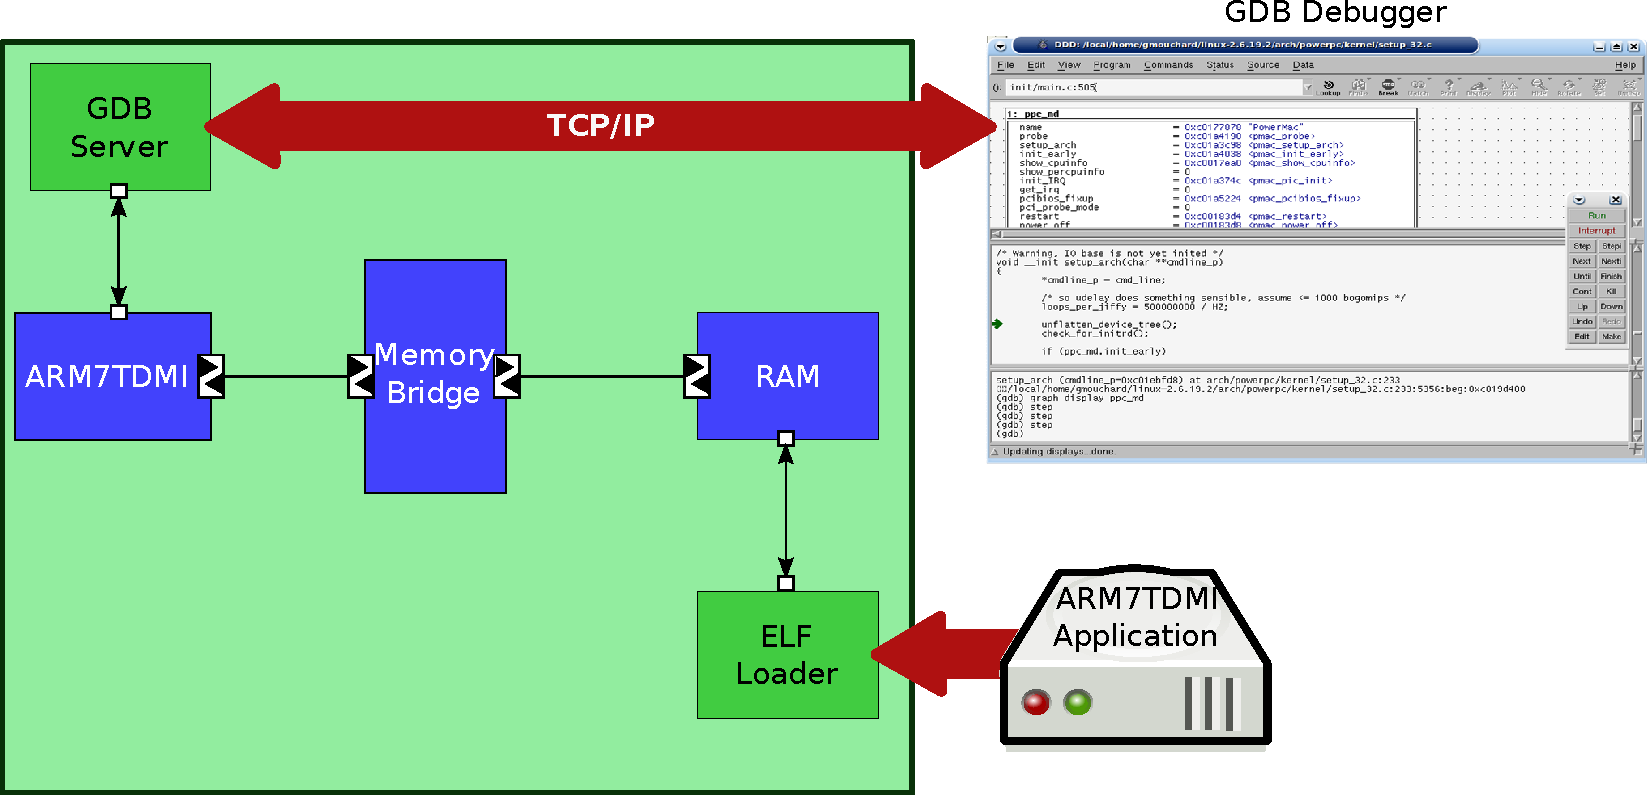
\includegraphics[width=\textwidth]{arm7tdmi_validation/figures/ARM7TDMI_architecture.pdf}
	\end{center}
	\caption{ARM7TDMI schematic architecture.}
	\label{fig:arm7tdmi_architecture}
\end{figure}

Figure~\ref{fig:arm7tdmi_architecture} shows the schematic architecture of the simulator used for the validation of the ARM7TDMI processor.
The simulator itself consist on three components (the blue boxes on Figure~\ref{fig:arm7tdmi_architecture}):
\begin{itemize}
	\item \textbf{ARM7TDMI:} this component models the ARM7TDMI processor itself.
	\item \textbf{Memory Bridge:} this component allows the connection of the ARM7TDMI processor to the main memory.
	\item \textbf{RAM:} this component is the memory of the system. The processor uses it to load the program to run and store temporary information.
\end{itemize}

Additionally, the simulator provides two services (green boxes on Figure~\ref{fig:arm7tdmi_architecture}):
\begin{itemize}
	\item \textbf{ELF Loader:} thanks to this service ARM7TDMI binaries can be loaded into the RAM component.
	\item \textbf{GDB Server:} this service enables extended debugging with the help of an external client debugger, as for example: gdb, ddd, eclipse debugger, and others.
\end{itemize}


\section{Tools}
\label{sec:tools}

For the validation of the ARM7TDMI simulator the following tools were used:
\begin{itemize}
	\item Random test generator: tool created at CEA to create random tests from an input template. It is briefly described in Section~\ref{sec:random_tests}.
	\item GNU compilations tools for ARM:
	\begin{itemize}
		\item GCC version 3.4.5 (C compiler)
		\item AS version 2.15 (Assembler compiler)
		\item LD version 2.15 (Linker)
	\end{itemize}
	\item GNU debugger for ARM: gdb version 6.1.1
	\item Linksys NSLU2 containing an ARM9 microprocessor. This is the target platform to validate the simulator against.
\end{itemize}


\section{User Level ISA Validation}
\label{sec:user_level}

When performing the validation of the ISA at the \textit{user level} we are only interested in the instructions that the processor can execute when running at the \textit{user mode}.
The \textit{user mode} is usually the most used mode on a processor (whenever the processor has multiple execution modes, which the ARM7TDMI has).
It is used to run the non-system dependent part of the applications.
Whenever an application needs to access the system (write on the screen, read the input from the keyboard, etc), it executes an special instruction (usually we call it \textit{system call}) which switches the processor to \textit{system mode} to perform the required operation.

The interest on performing a validation of \textit{user level} instructions resides on the difficulty to perform complete tests when using the \textit{system level} instructions (as we will see on Section~\ref{sec:system_level}).

\begin{figure}[!h]
	\begin{center}
		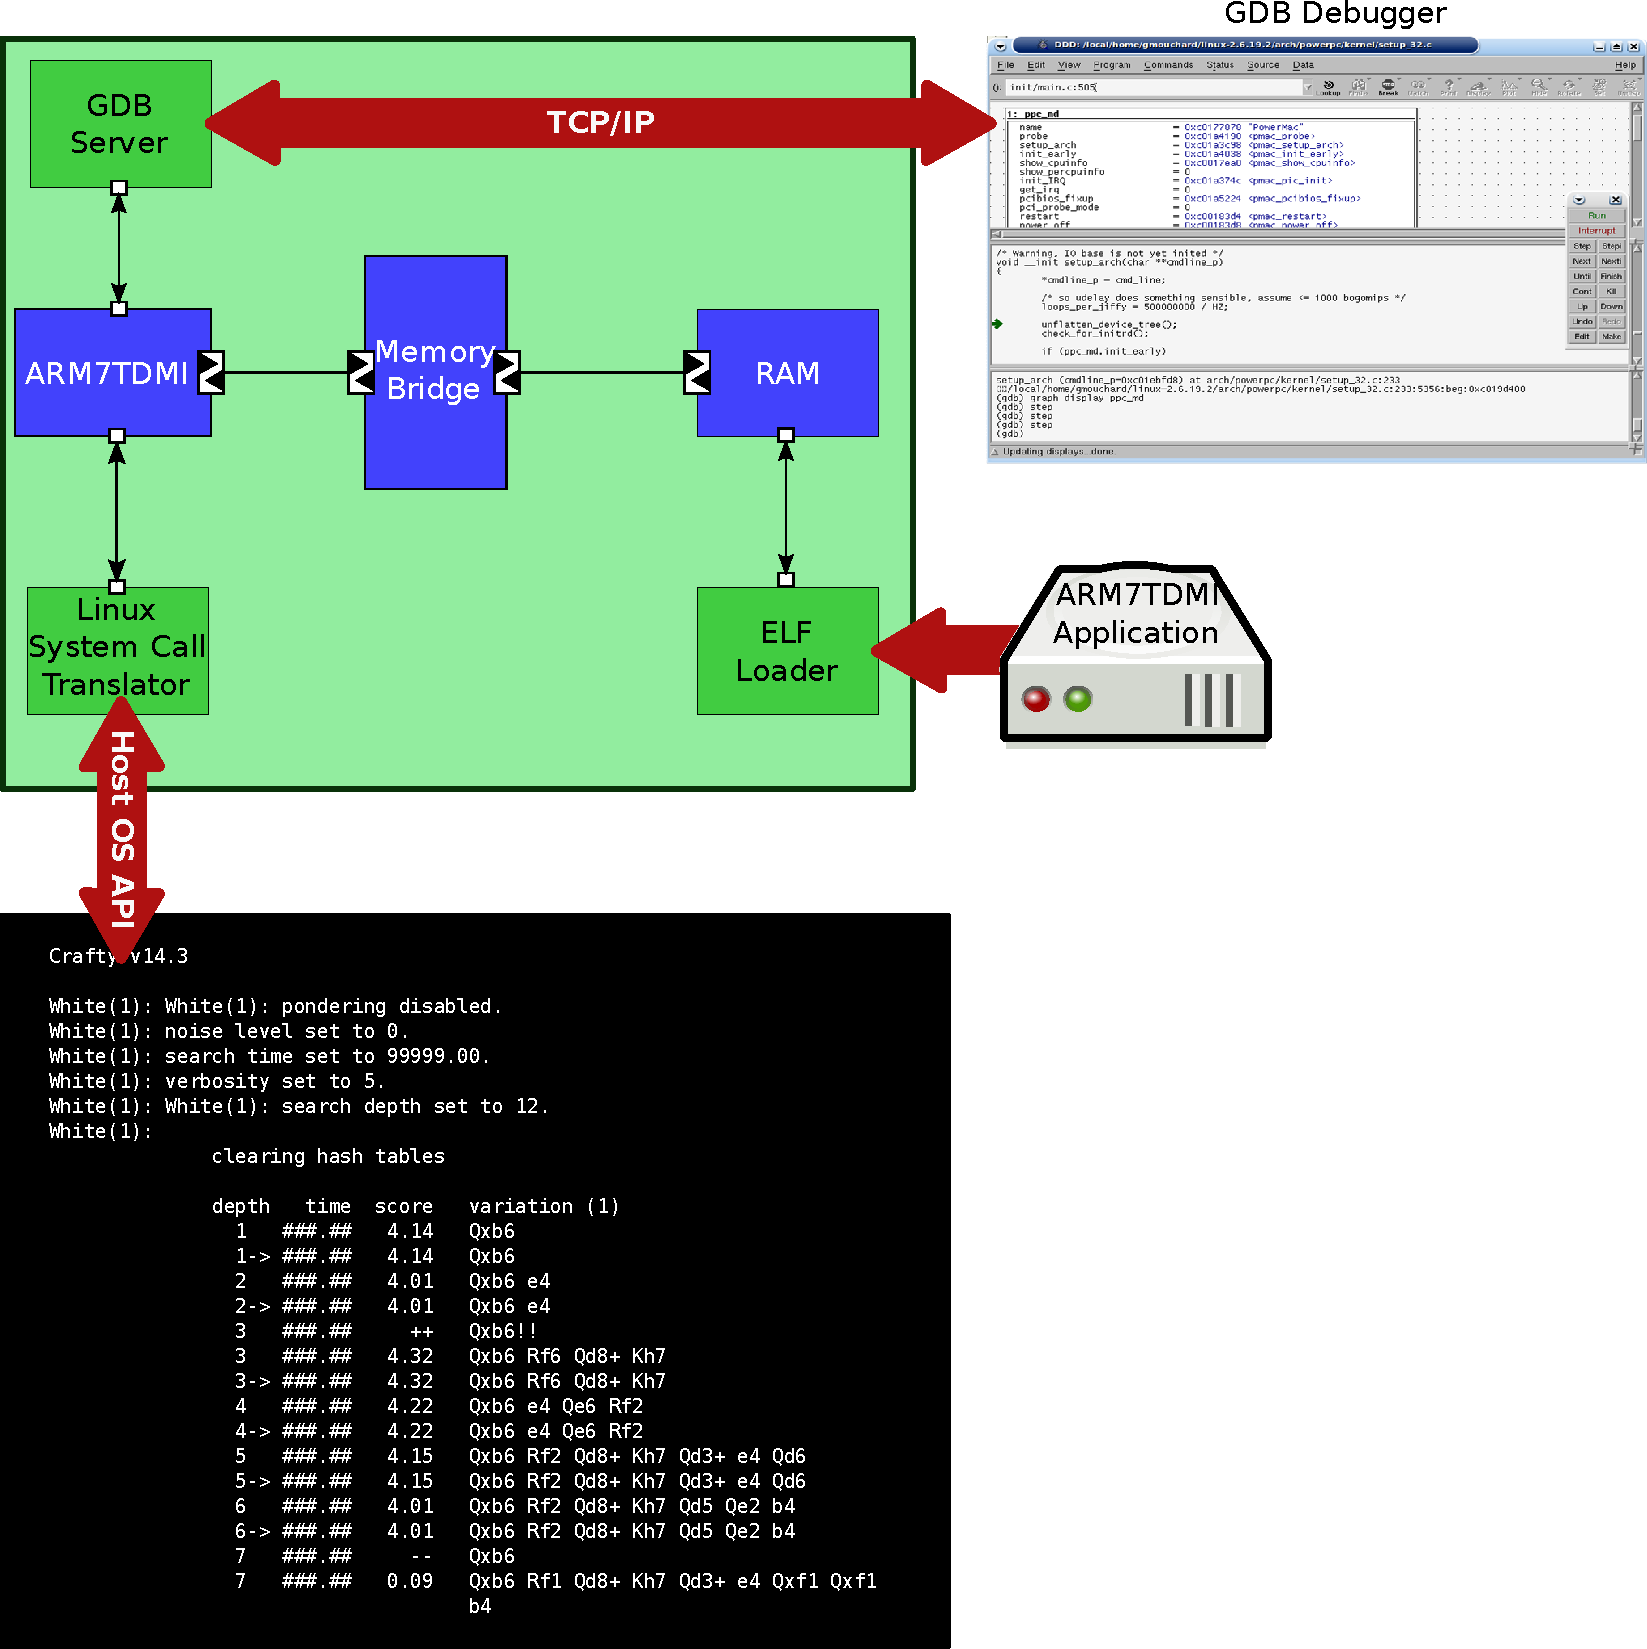
\includegraphics[width=\textwidth]{arm7tdmi_validation/figures/ARM7TDMI_user_level.pdf}
	\end{center}
	\caption{ARM7TDMI schematic architecture to run applications at user level.}
	\label{fig:arm7tdmi_user_level}
\end{figure}

In order to validate only the \textit{user level} ISA, the simulator is run with a special configuration, see Figure~\ref{fig:arm7tdmi_user_level}.
To the \textit{ELF Loader} and the \textit{GDB Server} services a third service has been added: the \textit{Linux System Call Translator}.
This service takes control of the simulation when a system call is executed, providing the program being executed by the simulator a translation of the system calls, without having to execute any system level instruction.
More concreatelly, the \textit{Linux System Call Translator} provides a traduction to Linux programs, which means that programs running under this configuration need to be compiled for ARM Linux.

\begin{figure}[!h]
	\begin{center}
		\includegraphics[width=\textwidth]{arm7tdmi_validation/figures/random_tests_methodology.pdf}
	\end{center}
	\caption{Random tests methodology.}
	\label{fig:random_tests_methodology}
\end{figure}

Figure~\ref{fig:random_tests_methodology} shows the steps taken to perform the validation of the user level ISA.
Once the simulator is written an application is run into booth the simulator and the target platform.
The output results of the simulator and the target platform are then compared.
If results match then it means that the simulator is correctly implemented.
If the results do not match we debug the simulator to fix it using the results differences, and the previous steps are repeated until the results match.

The following two subsections presents different validation tests performed under this configuration.
As target platform we used an ARM9 platform.
While it is not an ARM7TDMI platform, the ARM9 shares the same instructions at the user level, making it a valid target platform for the ARM7TDMI simulator at the user level.

\subsection{Random Tests}
\label{sec:random_tests}

The validation of all the instructions is an impossible task as it would mean to check all the instructions with all the possible inputs.
So in order to create an extensive and systematic validation of all the instructions we have created a small tool to generate random tests.
The tool takes as input a template describing the instruction to test, but not defining the instruction inputs.
The tool then creates multiple tests of the instruction defining random inputs.
The outputs of the tests are printed on the screen, so we can compare the outputs of the simulator against those of the target platform.

\begin{figure}[!h]
	\input{arm7tdmi_validation/adc_imm}
	\caption{\texttt{adc} with immediate input template.}
	\label{fig:adc_imm_template}
\end{figure}

Figure~\ref{fig:adc_imm_template} shows an example of template for the \texttt{adc} instruction using an immediate as input.
Line \texttt{1} sets to 0 the \texttt{r9} register which will be used later for storing the result of the \texttt{adc} instruction.
Lines \texttt{2}, \texttt{3} and \texttt{4} set randomly the status bits of the \texttt{cpsr} register which may influence the computation of the \texttt{adc} instruction.
Line \texttt{5} is the actual test of the \texttt{adc} instruction. 
The \texttt{\%(,eq,ne,...)} string appends nothing or one of the guarding pnemonics to the \texttt{adc} instruction, which one is selected randomly by the random tests generator.
Similarly the \texttt{\%(,s)} string appends nothing or the ``\texttt{s}'' string to the \texttt{adc} instruction.
The ``\texttt{s}'' flag indicates that the \texttt{cpsr} register should be updated if present, or leaved untouched otherwise.
The result of the \texttt{adc} instruction is stored in the \texttt{r9} register.
The \texttt{adc} uses two different inputs: a register and an immediate.
The register input is generated randomly by the test generator with the ``\texttt{\%r}'' string, choosing randomly one of the available registers and setting it to a random generated value.
The immediate input is generated randomly with the ``\texttt{\%s8,4,2}'' string\footnote{We are not going to get into details on how the immediate value is defined, just mention that it generates an integer that can be accepted by the ARM7 compiler.}.
Finally, lines \texttt{6}, \texttt{7} and \texttt{8} store the maybe modified \texttt{cpsr} status flags into a register chosen by the test generator (indicated with the ``\texttt{\%R}'').
Similarly, in line \texttt{9}, the register \texttt{r9} is copied into a register chosen by the test generator.
The registers marked with the ``\texttt{\%R}'' are then printed into the terminal, so we can compare the outputs from the simulation and the execution on ARM9 platform.
For each instruction test we check that the output register and the \texttt{cpsr} flags are correctly set.

\subsubsection{Results}

Test templates as the one presented in Figure~\ref{fig:adc_imm_template} have been developed for all the versions of the \texttt{adc} instruction (i.e., with two input registers, with a shifted immediate as input, and with a shifted register as input), and for all of the versions of most of the \textit{user level} instructions of the ARM7TDMI.
A total of 100,000 tests were generated from each template (making an average of 400,000 tests for instruction), and all the tests were succesfully passed. The following is a list of the validated instructions:
\begin{enumerate}
	\item adc
	\item add
	\item and
	\item bic
	\item cmn
	\item cmp
	\item eor
	\item mla
	\item mov
	\item mul
	\item mvn
	\item orr
	\item rsb
	\item rsc
	\item sbc
	\item smlal
	\item smull
	\item sub
	\item teq
	\item tst
	\item umlal
	\item umull
\end{enumerate}

This list includes all the \textit{user level} instructions of the ARM7TDMI processor, with the exception of memory instructions, branch instructions, and the system call instruction.
To validate those instructions (and complete the validation of the \textit{user level} instructions tested by the random tests), we performed tests over full applications presented in the following section.


\subsection{Benchmark Suite}
\label{sec:benchmark_suite}

While the validation performed in the previous section ensures the correct individual behavior of the tested instructions, it does not test the interaction between them, and some instructions are still missing, like all the load/store instructions, branch instructions, and the system call instruction.
To test the missing instructions and their interactions different real world applications are better suited.

The applications used for this validation are the SPEC2000 CINT.
The following is a list of the applications used with a small description extracted from the SPEC2000 documentation:
\begin{itemize}
	\item \textbf{gzip:} gzip (GNU zip) is a popular data compression program written by Jean-Loup Gailly $<$gzip@gnu.org$>$ for the GNU project. gzip uses Lempel-Ziv coding (LZ77) as its compression algorithm.
	\item \textbf{vpr:} VPR is a placement and routing program; it automatically implements a technology-mapped circuit (i.e. a netlist, or hypergraph, composed of FPGA logic blocks and I/O pads and their required connections) in a Field-Programmable Gate Array (FPGA) chip.  VPR is an example of an integrated circuit computer-aided design program, and algorithmically it belongs to the combinatorial optimization class of programs.
	\item \textbf{gcc:} this application is based on gcc Version 2.7.2.2. It generates code for a Motorola 88100 processor. The benchmark runs as a compiler with many of its optimization flags enabled.
	\item \textbf{mcf:} a benchmark derived from a program used for single-depot vehicle scheduling in public mass transportation. The program is written in C, the benchmark version uses almost exclusively integer arithmetic.
	\item \textbf{crafty:} Crafty is a high-performance Computer Chess program that is designed around a 64bit word. It runs on 32 bit machines using the ``long long'' (or similar, as \_int64 in Microsoft C) data type.  It is primarily an integer code, with a significant number of logical operations such as and, or, exclusive or and shift.  It can be configured to run a reproducible set of searches to compare the integer/branch prediction/pipe-lining facilities of a processor.
	\item \textbf{parser:} parser does the grungy job of chopping the user's input sentence into words, processing the special commands, and calling all the functions necessary to parse the input sentence.
	\item \textbf{eon:} Eon is a probabilistic ray tracer based on Kajiya's 1986 ACM SIGGRAPH conference paper. It sends a number of 3D lines (rays) into a 3D polygonal model. Intersections between the lines and the polygons are computed, and new lines are generated to compute light incident at these intersection points. The final result of the computation is an image as seen by camera. The computational demands of the program are much like a traditional deterministic ray tracer as described in basic computer graphics texts, but it has less memory coherence because many of the random rays generated in the same part of the code traverse very different parts of 3D space.
	\item \textbf{perlbmk:} perlbmk is a cut-down version of Perl v5.005\_03, the popular scripting language. SPEC's version of Perl has had most of OS-specific features removed.
	\item \textbf{gap:} gap implements a language and library designed mostly for computing in groups (GAP is an acronym for Groups, Algorithms and Programming).
	\item \textbf{vortex:} VORTEx is a single-user object-oriented database transaction benchmark  which which exercises a system kernel coded in integer C.
	\item \textbf{bzip2:} bzip2 is based on Julian Seward's bzip2 version 0.1. The only difference between bzip2 0.1 and bzip2 is that SPEC's version of bzip2 performs no file I/O other than reading the input. All compression and decompression happens entirely in memory. This is to help isolate the work done to only the CPU and memory subsystem.
	\item \textbf{twolf:} The TimberWolfSC placement and global routing package is used in the process of creating the lithography artwork needed for the production of microchips. Specifically, it determines the placement and global connections for groups of transistors (known as standard cells) which constitute the microchip. The placement problem is a permutation. The TimberWolfSC program (twolf) uses simulated annealing as a heuristic to find very good solutions for the row-based standard cell design style.  In this design style, transistors are grouped together to form standard cells.
\end{itemize}

All these applications were developed in order to stress the cpu and the memory system, which covers the memory and branch instructions validation missing in the random tests presented in Section~\ref{sec:random_tests}. 
Additionally, while not in an intensive manner, those applications test the functionality of the system call instruction.

\subsubsection{Results}

All those applications have been successfully run in the ARM7TDMI simulator, and their outputs match those of to the target plaform.
Three different input sets (provided with the SPEC2000) have been used for each of the application:
\begin{itemize}
	\item \textbf{train:} small input set that has been mainly used during the development of the simulator.
	\item \textbf{test:} medium size input set.
	\item \textbf{ref:} large size input set, recommended by the SPEC2000 manual to fully stress the CPU and the memory system.
\end{itemize}

All the SPEC2000 applications were used during the development of the simulator, and no other tests were performed until all of them were successfully simulated.
After that the random tests (see Section~\ref{sec:random_tests}) were performed founding only one error (with the \texttt{mrc} instruction).
Finally, the system test presented in the following Section were performed to validate the system level behavior of the ARM7TDMI simulator.




\section{System Level Validation}
\label{sec:system_level}

The tests presented in Section~\ref{sec:user_level} validated the user level ISA subset of the complete ARM7TDMI ISA.
Validation of the system level ISA is a more complicated.
Firstly, systematic tests as the random tests introduced in Section~\ref{sec:random_tests} are not feasible, due to the system dependencies of those instructions.
Secondly, there are not benchmarks as those presented in Section~\ref{sec:benchmark_suite} to validate the ARM7TDMI alone.
System benchmarks exist, but they require more components than those developed for the architecture targeted in this document (see Figure~\ref{fig:arm7tdmi_architecture}).

For those reasons we have developed a small kernel to test the following features of the system:
\begin{itemize}
	\item system bootup
	\item exception mechanism
	\item user/system mode switching
	\item ARM ISA to Thumb ISA switching
\end{itemize}

\subsection{Results}
To validate the behavior of the ARM7TDMI simulator at system level we do not have any tool to do it automatically (we can not compare two outputs like presented in Section~\ref{sec:user_level}).
We performed all the validation manually, heavily using the debugging service provided with UNISIM and comparing the behavior of the simulator to the behavior described in the ARM manual.
All the tests were succesfully validated.


\section{Conclusion}
\label{sec:conclusion}

This document has presented the different tests that have been performed in order to validate the ARM7TDMI simulator.
With the SPEC2000 application suit the simulator have been validated to be used with real world applications.
Thanks to the random tests technique developped at CEA an extensive validation of all the ARM7TDMI user level instructions have been done.
Finally, with the development of a small kernel the simulator has been validated for the execution of system level applications, like operating systems, drivers, and embedded applications.

As for any software application, the validation does not ensure that the simulator is bug free.
However, the validation performed ensures that the simulator functionality matches the ARM7TDMI functionality, and that any application can be run on it with confidence.
Additionally, the ARM7TDMI simulator provided in UNISIM (\url{http://www.unisim.org}) is open source, which means that users can fixe it if necessary and that corrections to the simulator can be easily shared.




\chapter{Validation of the UNISIM STR7 Microcontroller Simulator}
\label{str7_validation}
\subsection {Eléments de contexte}
Au cours de mon cursus à l'Ecole d'ingénieur Denis Diderot, j'ai eu l'occasion d'effectuer un stage de 6 mois entre la 2 ième et 3 ième année. 
J'ai donc choisi d'effectuer ce stage au C.E.A List afin d'avoir une expérience professionelle dans un organisme de recherche en informatique et de développer de nouvelles connaissances dans le domaine des systèmes embarqués.
Ma formation étant spécialisé dans la conception de logiciels embarqués et ayant suivi des cours d'architecture des processeurs, 
j'ai pensé qu'il serai intéressant d'approfondir mes connaissances dans le fonctionnenent des processeur afin d'avoir une vision plus complète de l'éxecution des programmes (niveau assembleur).
Gilles Mouchard et Reda Nouacer de l'équipe UNISIM recherchaient un étudiant afin d'effectuer un stage de 6 mois consistant à réaliser un simulateur de jeu d'instruction (ISS) d'un proceseur embarqué. 
\subsection{Contenue du document}
Ce document décrit le travail réalisé au cours de ce stage pendant la période du 10 mars au 31 août 2014 au sein du laboratoire LSL du CEA LIST.
Après une brève présentation du laboratoire et de l'équipe, j'établirai un  état de l'art sur les méthodes de conception et validation d'un simulateur suivie la présentation des outils utilisés pour le projet.
Puis je décrirai les étapes de réalisation et les résulats obtenues sur le processeur choisie par l'équipe.
J'évoquerai également les problèmes rencontrés et les moyens pour les résoudre. 
Enfin j'établirai un bilan sur les connaissances acquises durant ce stage concernant la simulation mais aussi plus généralement sur les méthodes de développement de logiciel.      

\section{The ARM7TDMI Microprocessor Simulator Description}

The ARM7TDMI core is a member of the ARM family of general-purpose 32-bit microprocessors.
The ARM family offers high performance for very low power consumption, and small size.

The ARM7TDMI architecture is based on \textit{Reduced Instruction Set Computer} (RISC) principles.
It uses a three-stage pipeline, so instructions are executed in three stages:
\begin{itemize}
	\item Fetch: instruction fetched from memory.
	\item Decode: decoding of registers used in instruction.
	\item Execute: register(s) read from register bank, shift and/or ALU operation, write register(s) back to register bank.
\end{itemize}
A total of 32 registers are available.
However, the processor has seven modes of execution, and while executing in a given mode the processor has only access to a subset (concretely sixteen registers) of them.
Additionally, the ARM7TDMI can execute two different instruction sets (ISAs):
\begin{itemize}
	\item Standard ARM ISA: it is composed of 32 bits RISC instructions. This is the main ISA of the ARM processors series.
	\item Thumb ISA: it is composed of 16 bits RISC instructions. This ISA is used to reduce code footprint, however the number of instructions proposed by this ISA is reduced, so not all kind of operations can done using this ISA.
\end{itemize}
The two ISAs are fully supported by the simulator.

For the development of the ARM7TDMI simulator developed at CEA LIST the following documents were used:
\begin{itemize}
	\item ARM Architecture Reference Manual
	\item ARM7TDMI (Rev 4) Technical Reference Manual
\end{itemize}
Please refer to them if you are looking for more details on the ARM7TDMI processor.

\begin{figure}[!h]
	\begin{center}
		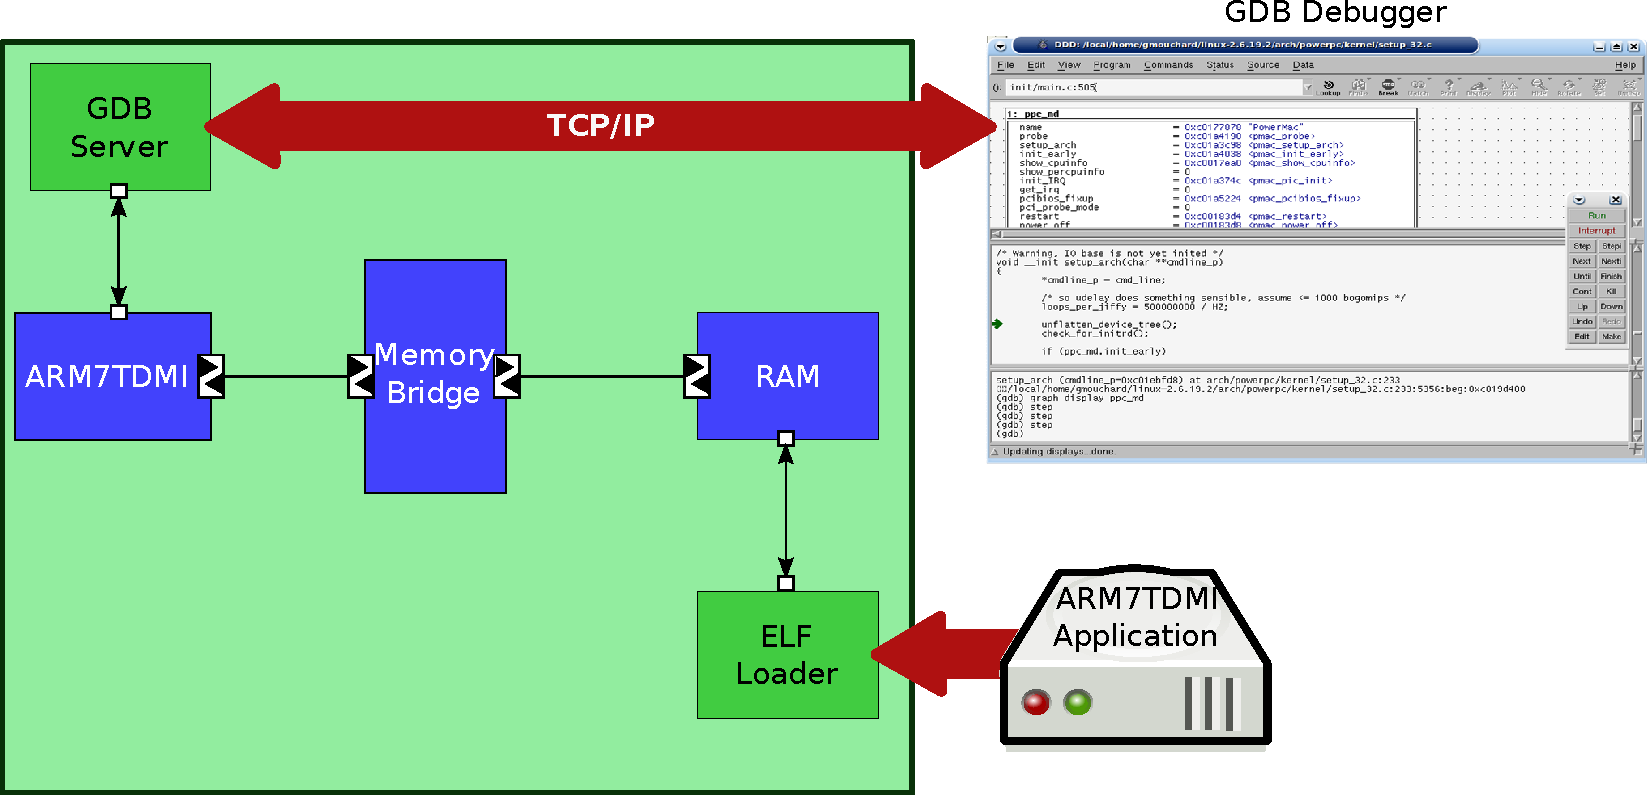
\includegraphics[width=\textwidth]{arm7tdmi_validation/figures/ARM7TDMI_architecture.pdf}
	\end{center}
	\caption{ARM7TDMI schematic architecture.}
	\label{fig:arm7tdmi_architecture}
\end{figure}

Figure~\ref{fig:arm7tdmi_architecture} shows the schematic architecture of the simulator used for the validation of the ARM7TDMI processor.
The simulator itself consist on three components (the blue boxes on Figure~\ref{fig:arm7tdmi_architecture}):
\begin{itemize}
	\item \textbf{ARM7TDMI:} this component models the ARM7TDMI processor itself.
	\item \textbf{Memory Bridge:} this component allows the connection of the ARM7TDMI processor to the main memory.
	\item \textbf{RAM:} this component is the memory of the system. The processor uses it to load the program to run and store temporary information.
\end{itemize}

Additionally, the simulator provides two services (green boxes on Figure~\ref{fig:arm7tdmi_architecture}):
\begin{itemize}
	\item \textbf{ELF Loader:} thanks to this service ARM7TDMI binaries can be loaded into the RAM component.
	\item \textbf{GDB Server:} this service enables extended debugging with the help of an external client debugger, as for example: gdb, ddd, eclipse debugger, and others.
\end{itemize}


\section{Tools}
\label{sec:tools}

For the validation of the ARM7TDMI simulator the following tools were used:
\begin{itemize}
	\item Random test generator: tool created at CEA to create random tests from an input template. It is briefly described in Section~\ref{sec:random_tests}.
	\item GNU compilations tools for ARM:
	\begin{itemize}
		\item GCC version 3.4.5 (C compiler)
		\item AS version 2.15 (Assembler compiler)
		\item LD version 2.15 (Linker)
	\end{itemize}
	\item GNU debugger for ARM: gdb version 6.1.1
	\item Linksys NSLU2 containing an ARM9 microprocessor. This is the target platform to validate the simulator against.
\end{itemize}


\section{User Level ISA Validation}
\label{sec:user_level}

When performing the validation of the ISA at the \textit{user level} we are only interested in the instructions that the processor can execute when running at the \textit{user mode}.
The \textit{user mode} is usually the most used mode on a processor (whenever the processor has multiple execution modes, which the ARM7TDMI has).
It is used to run the non-system dependent part of the applications.
Whenever an application needs to access the system (write on the screen, read the input from the keyboard, etc), it executes an special instruction (usually we call it \textit{system call}) which switches the processor to \textit{system mode} to perform the required operation.

The interest on performing a validation of \textit{user level} instructions resides on the difficulty to perform complete tests when using the \textit{system level} instructions (as we will see on Section~\ref{sec:system_level}).

\begin{figure}[!h]
	\begin{center}
		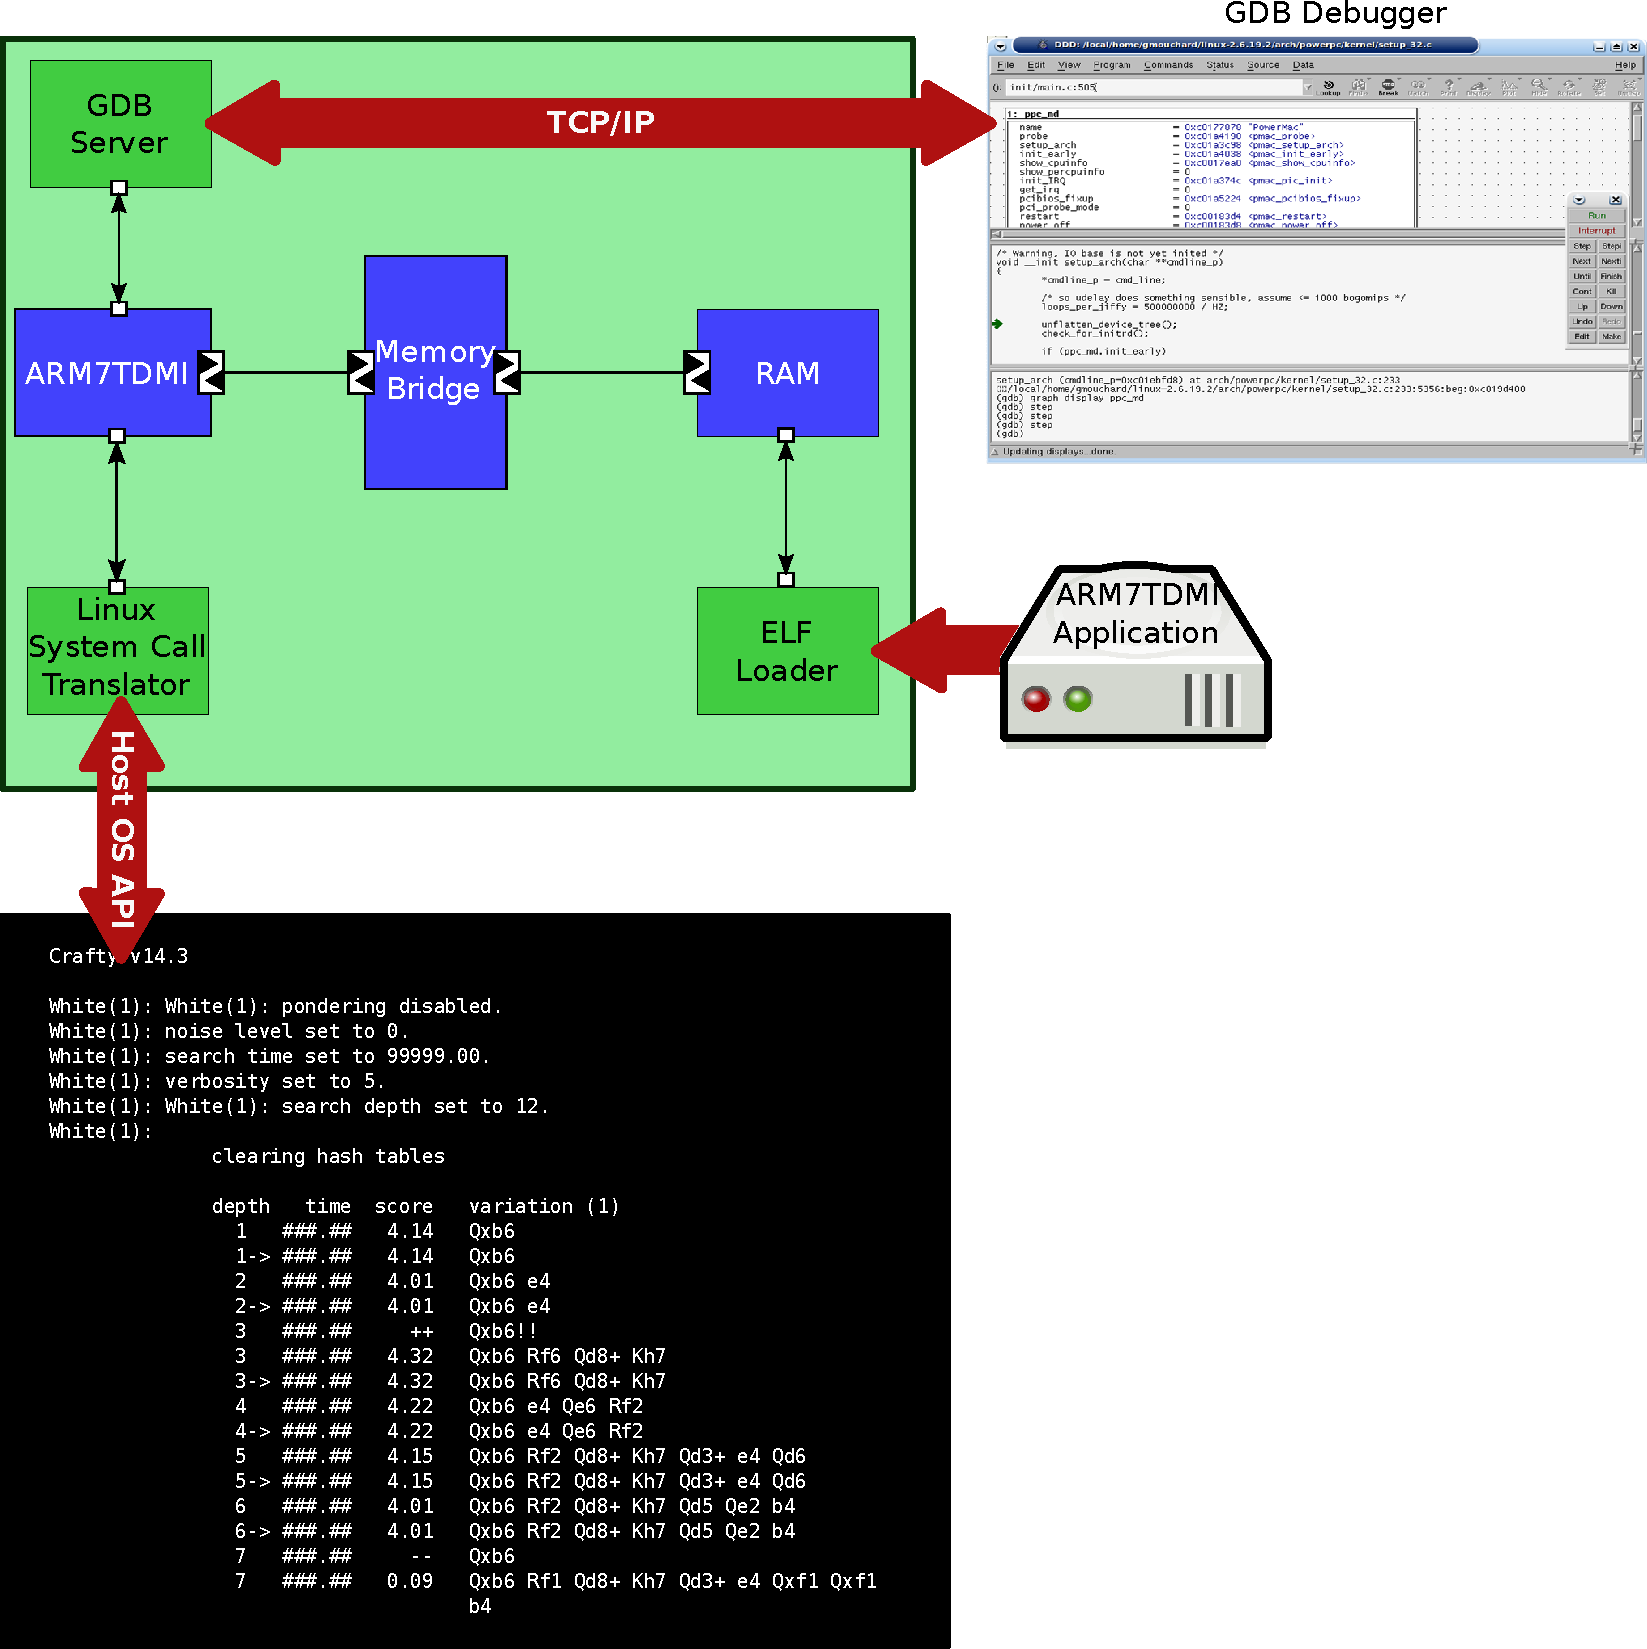
\includegraphics[width=\textwidth]{arm7tdmi_validation/figures/ARM7TDMI_user_level.pdf}
	\end{center}
	\caption{ARM7TDMI schematic architecture to run applications at user level.}
	\label{fig:arm7tdmi_user_level}
\end{figure}

In order to validate only the \textit{user level} ISA, the simulator is run with a special configuration, see Figure~\ref{fig:arm7tdmi_user_level}.
To the \textit{ELF Loader} and the \textit{GDB Server} services a third service has been added: the \textit{Linux System Call Translator}.
This service takes control of the simulation when a system call is executed, providing the program being executed by the simulator a translation of the system calls, without having to execute any system level instruction.
More concreatelly, the \textit{Linux System Call Translator} provides a traduction to Linux programs, which means that programs running under this configuration need to be compiled for ARM Linux.

\begin{figure}[!h]
	\begin{center}
		\includegraphics[width=\textwidth]{arm7tdmi_validation/figures/random_tests_methodology.pdf}
	\end{center}
	\caption{Random tests methodology.}
	\label{fig:random_tests_methodology}
\end{figure}

Figure~\ref{fig:random_tests_methodology} shows the steps taken to perform the validation of the user level ISA.
Once the simulator is written an application is run into booth the simulator and the target platform.
The output results of the simulator and the target platform are then compared.
If results match then it means that the simulator is correctly implemented.
If the results do not match we debug the simulator to fix it using the results differences, and the previous steps are repeated until the results match.

The following two subsections presents different validation tests performed under this configuration.
As target platform we used an ARM9 platform.
While it is not an ARM7TDMI platform, the ARM9 shares the same instructions at the user level, making it a valid target platform for the ARM7TDMI simulator at the user level.

\subsection{Random Tests}
\label{sec:random_tests}

The validation of all the instructions is an impossible task as it would mean to check all the instructions with all the possible inputs.
So in order to create an extensive and systematic validation of all the instructions we have created a small tool to generate random tests.
The tool takes as input a template describing the instruction to test, but not defining the instruction inputs.
The tool then creates multiple tests of the instruction defining random inputs.
The outputs of the tests are printed on the screen, so we can compare the outputs of the simulator against those of the target platform.

\begin{figure}[!h]
	\input{arm7tdmi_validation/adc_imm}
	\caption{\texttt{adc} with immediate input template.}
	\label{fig:adc_imm_template}
\end{figure}

Figure~\ref{fig:adc_imm_template} shows an example of template for the \texttt{adc} instruction using an immediate as input.
Line \texttt{1} sets to 0 the \texttt{r9} register which will be used later for storing the result of the \texttt{adc} instruction.
Lines \texttt{2}, \texttt{3} and \texttt{4} set randomly the status bits of the \texttt{cpsr} register which may influence the computation of the \texttt{adc} instruction.
Line \texttt{5} is the actual test of the \texttt{adc} instruction. 
The \texttt{\%(,eq,ne,...)} string appends nothing or one of the guarding pnemonics to the \texttt{adc} instruction, which one is selected randomly by the random tests generator.
Similarly the \texttt{\%(,s)} string appends nothing or the ``\texttt{s}'' string to the \texttt{adc} instruction.
The ``\texttt{s}'' flag indicates that the \texttt{cpsr} register should be updated if present, or leaved untouched otherwise.
The result of the \texttt{adc} instruction is stored in the \texttt{r9} register.
The \texttt{adc} uses two different inputs: a register and an immediate.
The register input is generated randomly by the test generator with the ``\texttt{\%r}'' string, choosing randomly one of the available registers and setting it to a random generated value.
The immediate input is generated randomly with the ``\texttt{\%s8,4,2}'' string\footnote{We are not going to get into details on how the immediate value is defined, just mention that it generates an integer that can be accepted by the ARM7 compiler.}.
Finally, lines \texttt{6}, \texttt{7} and \texttt{8} store the maybe modified \texttt{cpsr} status flags into a register chosen by the test generator (indicated with the ``\texttt{\%R}'').
Similarly, in line \texttt{9}, the register \texttt{r9} is copied into a register chosen by the test generator.
The registers marked with the ``\texttt{\%R}'' are then printed into the terminal, so we can compare the outputs from the simulation and the execution on ARM9 platform.
For each instruction test we check that the output register and the \texttt{cpsr} flags are correctly set.

\subsubsection{Results}

Test templates as the one presented in Figure~\ref{fig:adc_imm_template} have been developed for all the versions of the \texttt{adc} instruction (i.e., with two input registers, with a shifted immediate as input, and with a shifted register as input), and for all of the versions of most of the \textit{user level} instructions of the ARM7TDMI.
A total of 100,000 tests were generated from each template (making an average of 400,000 tests for instruction), and all the tests were succesfully passed. The following is a list of the validated instructions:
\begin{enumerate}
	\item adc
	\item add
	\item and
	\item bic
	\item cmn
	\item cmp
	\item eor
	\item mla
	\item mov
	\item mul
	\item mvn
	\item orr
	\item rsb
	\item rsc
	\item sbc
	\item smlal
	\item smull
	\item sub
	\item teq
	\item tst
	\item umlal
	\item umull
\end{enumerate}

This list includes all the \textit{user level} instructions of the ARM7TDMI processor, with the exception of memory instructions, branch instructions, and the system call instruction.
To validate those instructions (and complete the validation of the \textit{user level} instructions tested by the random tests), we performed tests over full applications presented in the following section.


\subsection{Benchmark Suite}
\label{sec:benchmark_suite}

While the validation performed in the previous section ensures the correct individual behavior of the tested instructions, it does not test the interaction between them, and some instructions are still missing, like all the load/store instructions, branch instructions, and the system call instruction.
To test the missing instructions and their interactions different real world applications are better suited.

The applications used for this validation are the SPEC2000 CINT.
The following is a list of the applications used with a small description extracted from the SPEC2000 documentation:
\begin{itemize}
	\item \textbf{gzip:} gzip (GNU zip) is a popular data compression program written by Jean-Loup Gailly $<$gzip@gnu.org$>$ for the GNU project. gzip uses Lempel-Ziv coding (LZ77) as its compression algorithm.
	\item \textbf{vpr:} VPR is a placement and routing program; it automatically implements a technology-mapped circuit (i.e. a netlist, or hypergraph, composed of FPGA logic blocks and I/O pads and their required connections) in a Field-Programmable Gate Array (FPGA) chip.  VPR is an example of an integrated circuit computer-aided design program, and algorithmically it belongs to the combinatorial optimization class of programs.
	\item \textbf{gcc:} this application is based on gcc Version 2.7.2.2. It generates code for a Motorola 88100 processor. The benchmark runs as a compiler with many of its optimization flags enabled.
	\item \textbf{mcf:} a benchmark derived from a program used for single-depot vehicle scheduling in public mass transportation. The program is written in C, the benchmark version uses almost exclusively integer arithmetic.
	\item \textbf{crafty:} Crafty is a high-performance Computer Chess program that is designed around a 64bit word. It runs on 32 bit machines using the ``long long'' (or similar, as \_int64 in Microsoft C) data type.  It is primarily an integer code, with a significant number of logical operations such as and, or, exclusive or and shift.  It can be configured to run a reproducible set of searches to compare the integer/branch prediction/pipe-lining facilities of a processor.
	\item \textbf{parser:} parser does the grungy job of chopping the user's input sentence into words, processing the special commands, and calling all the functions necessary to parse the input sentence.
	\item \textbf{eon:} Eon is a probabilistic ray tracer based on Kajiya's 1986 ACM SIGGRAPH conference paper. It sends a number of 3D lines (rays) into a 3D polygonal model. Intersections between the lines and the polygons are computed, and new lines are generated to compute light incident at these intersection points. The final result of the computation is an image as seen by camera. The computational demands of the program are much like a traditional deterministic ray tracer as described in basic computer graphics texts, but it has less memory coherence because many of the random rays generated in the same part of the code traverse very different parts of 3D space.
	\item \textbf{perlbmk:} perlbmk is a cut-down version of Perl v5.005\_03, the popular scripting language. SPEC's version of Perl has had most of OS-specific features removed.
	\item \textbf{gap:} gap implements a language and library designed mostly for computing in groups (GAP is an acronym for Groups, Algorithms and Programming).
	\item \textbf{vortex:} VORTEx is a single-user object-oriented database transaction benchmark  which which exercises a system kernel coded in integer C.
	\item \textbf{bzip2:} bzip2 is based on Julian Seward's bzip2 version 0.1. The only difference between bzip2 0.1 and bzip2 is that SPEC's version of bzip2 performs no file I/O other than reading the input. All compression and decompression happens entirely in memory. This is to help isolate the work done to only the CPU and memory subsystem.
	\item \textbf{twolf:} The TimberWolfSC placement and global routing package is used in the process of creating the lithography artwork needed for the production of microchips. Specifically, it determines the placement and global connections for groups of transistors (known as standard cells) which constitute the microchip. The placement problem is a permutation. The TimberWolfSC program (twolf) uses simulated annealing as a heuristic to find very good solutions for the row-based standard cell design style.  In this design style, transistors are grouped together to form standard cells.
\end{itemize}

All these applications were developed in order to stress the cpu and the memory system, which covers the memory and branch instructions validation missing in the random tests presented in Section~\ref{sec:random_tests}. 
Additionally, while not in an intensive manner, those applications test the functionality of the system call instruction.

\subsubsection{Results}

All those applications have been successfully run in the ARM7TDMI simulator, and their outputs match those of to the target plaform.
Three different input sets (provided with the SPEC2000) have been used for each of the application:
\begin{itemize}
	\item \textbf{train:} small input set that has been mainly used during the development of the simulator.
	\item \textbf{test:} medium size input set.
	\item \textbf{ref:} large size input set, recommended by the SPEC2000 manual to fully stress the CPU and the memory system.
\end{itemize}

All the SPEC2000 applications were used during the development of the simulator, and no other tests were performed until all of them were successfully simulated.
After that the random tests (see Section~\ref{sec:random_tests}) were performed founding only one error (with the \texttt{mrc} instruction).
Finally, the system test presented in the following Section were performed to validate the system level behavior of the ARM7TDMI simulator.




\section{System Level Validation}
\label{sec:system_level}

The tests presented in Section~\ref{sec:user_level} validated the user level ISA subset of the complete ARM7TDMI ISA.
Validation of the system level ISA is a more complicated.
Firstly, systematic tests as the random tests introduced in Section~\ref{sec:random_tests} are not feasible, due to the system dependencies of those instructions.
Secondly, there are not benchmarks as those presented in Section~\ref{sec:benchmark_suite} to validate the ARM7TDMI alone.
System benchmarks exist, but they require more components than those developed for the architecture targeted in this document (see Figure~\ref{fig:arm7tdmi_architecture}).

For those reasons we have developed a small kernel to test the following features of the system:
\begin{itemize}
	\item system bootup
	\item exception mechanism
	\item user/system mode switching
	\item ARM ISA to Thumb ISA switching
\end{itemize}

\subsection{Results}
To validate the behavior of the ARM7TDMI simulator at system level we do not have any tool to do it automatically (we can not compare two outputs like presented in Section~\ref{sec:user_level}).
We performed all the validation manually, heavily using the debugging service provided with UNISIM and comparing the behavior of the simulator to the behavior described in the ARM manual.
All the tests were succesfully validated.


\section{Conclusion}
\label{sec:conclusion}

This document has presented the different tests that have been performed in order to validate the ARM7TDMI simulator.
With the SPEC2000 application suit the simulator have been validated to be used with real world applications.
Thanks to the random tests technique developped at CEA an extensive validation of all the ARM7TDMI user level instructions have been done.
Finally, with the development of a small kernel the simulator has been validated for the execution of system level applications, like operating systems, drivers, and embedded applications.

As for any software application, the validation does not ensure that the simulator is bug free.
However, the validation performed ensures that the simulator functionality matches the ARM7TDMI functionality, and that any application can be run on it with confidence.
Additionally, the ARM7TDMI simulator provided in UNISIM (\url{http://www.unisim.org}) is open source, which means that users can fixe it if necessary and that corrections to the simulator can be easily shared.




\begin{appendix}
\chapter{TLM library}
\label{tlm_appendix}
\section{The message}
\section{The \texttt{ResponseListener} class}


\chapter{UNISIM Virtex 5 FXT Simulator technical reference (generated) }
\label{techref}
This documentation has been automatically generated from the simulator \texttt{UNISIM Virtex 5 FXT} version 1.0beta13 on Mar  4 2015.
\subsection{Introduction}
UNISIM Virtex 5 FXT, full system PPC440x5 based simulator including some Virtex 5 IPs.\\
Section \ref{UNISIM Virtex 5 FXT_licensing} gives licensing informations about the simulator.
Section \ref{UNISIM Virtex 5 FXT_simulated_configuration} shows the set of modules and services that compose the simulator.
Section \ref{UNISIM Virtex 5 FXT_using} shows how to invoke the simulator at the command line prompt.
Section \ref{UNISIM Virtex 5 FXT_configuration} gives the simulator parameters.
Section \ref{UNISIM Virtex 5 FXT_statistics} gives the simulator statistic counters.
Section \ref{UNISIM Virtex 5 FXT_formulas} gives the simulator statistic formulas.
\subsection{Licensing}
\label{UNISIM Virtex 5 FXT_licensing}
UNISIM Virtex 5 FXT 1.0beta13\\
Copyright (C) 2007-2011, Commissariat a l'Energie Atomique (CEA)\\
License: BSD (see file COPYING)\\
Authors: Gilles Mouchard $<$gilles.mouchard@cea.fr$>$, Daniel Gracia P\'erez $<$daniel.gracia-perez@cea.fr$>$\\
\subsection{Simulated configuration}
\label{UNISIM Virtex 5 FXT_simulated_configuration}
\begin{figure}[!ht]
	\begin{center}
		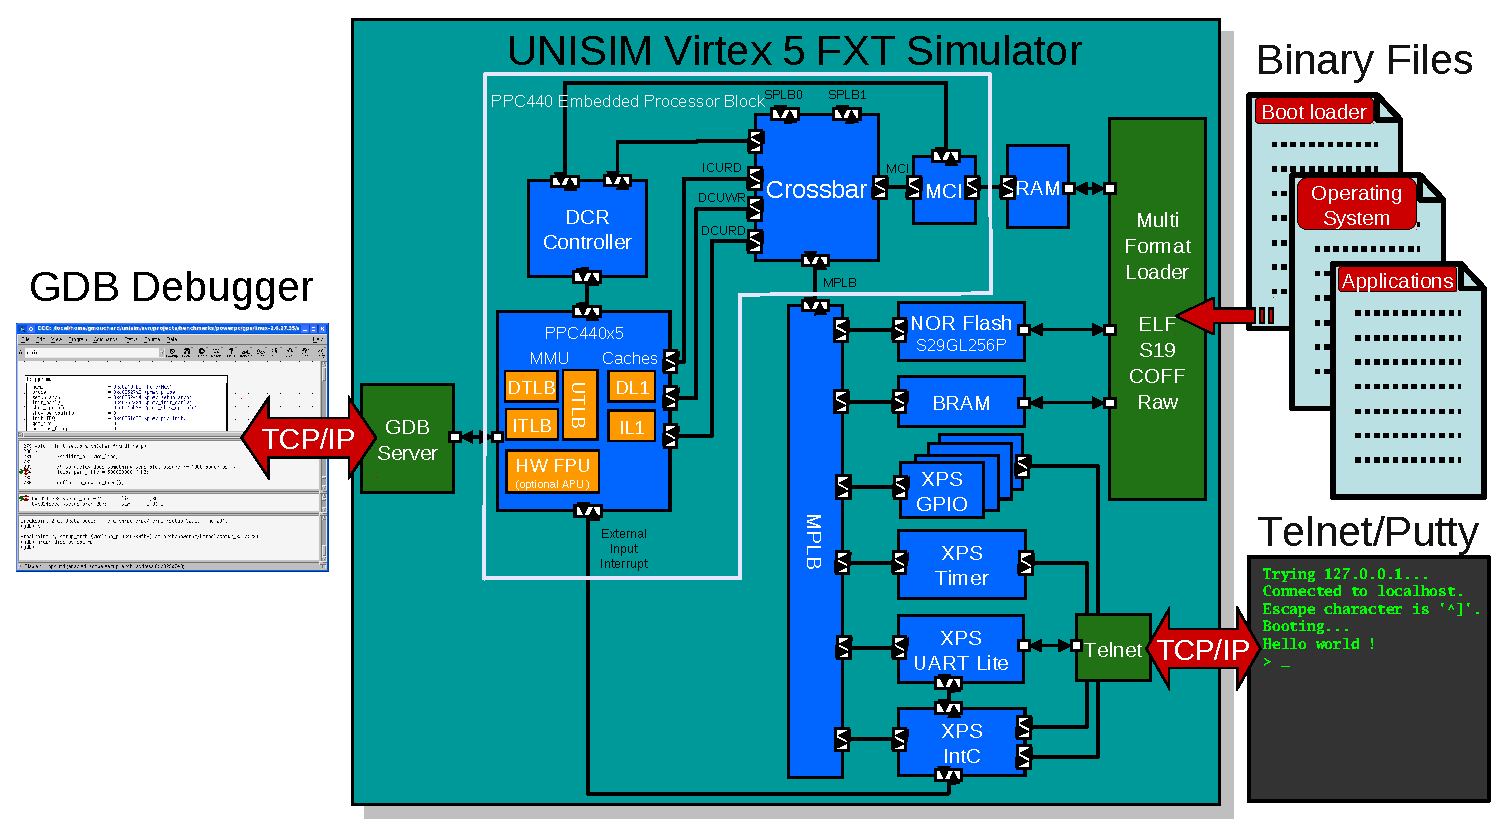
\includegraphics[width=\textwidth]{virtex5fxt/fig_schematic.pdf}
	\end{center}
	\caption{UNISIM Virtex 5 FXT simulator schematic.}
\end{figure}
\noindent The UNISIM Virtex 5 FXT simulator is composed of the following modules and services:
\begin{itemize}\addtolength{\itemsep}{-0.40\baselineskip}
\item \textbf{5-leds-positions}: This module implements a 5-LED board on GPIO.\\

\item \textbf{apu-dcr-stub}: A target stub
\item \textbf{bram}: this module implements a memory
\item \textbf{bram-effective-to-physical-address-translator}: this service translates memory addresses when playing with different address sizes
\item \textbf{capture-trigger-stub0}: A stub that, if enabled, can generate random inputs for a capture timer
\item \textbf{capture-trigger-stub1}: A stub that, if enabled, can generate random inputs for a capture timer
\item \textbf{cpu}: This module implements a PPC440 CPU core. It has the following characteristics:\\
Processor version (PVR value): 0x7ff21912\\
Reset configuration (RSTCFG): U0=0, U1=0, U2=0, U3=0, E=0, ERPN=0x0\\
Start address: 0xfffffffc\\
L1 data cache: size=32768 bytes, block size=32 bytes, associativity=64\\
L1 instruction cache: size=32768 bytes, block size=32 bytes, associativity=64\\
shadow instruction TLB: size=4 entries, associativity=4\\
shadow data TLB: size=8 entries, associativity=8\\
unified TLB: size=64 entries, associativity=64\\
FSB/PLB burst size:256 bits\\
FSB/PLB width:128 bits\\
MMU: yes\\
FPU APU: yes
\item \textbf{critical-input-interrupt-stub}: An initiator stub
\item \textbf{crossbar}: This module implements the crossbar of the embedded processor block in Virtex-5 FXT FPGAs from Xilinx. It has the following address mappings at reset:\\
ICURD mapping:\\
  - 0x0-0x7fffffff $\rightarrow$ MCI\\
  - 0x80000000-0xfffffffff $\rightarrow$ MPLB\\
DCUWR mapping:\\
  - 0x0-0x7fffffff $\rightarrow$ MCI\\
  - 0x80000000-0xfffffffff $\rightarrow$ MPLB\\
DCURD mapping:\\
  - 0x0-0x7fffffff $\rightarrow$ MCI\\
  - 0x80000000-0xfffffffff $\rightarrow$ MPLB\\
SPLB0 mapping:\\
  - 0x0-0xfffffffff $\rightarrow$ MCI\\
SPLB1 mapping:\\
  - 0x0-0xfffffffff $\rightarrow$ MCI\\

\item \textbf{dcr-controller}: A Device Control Register bus controller
\item \textbf{debugger}
\item \textbf{dip-switches-8bit}: This module implements a 8-switch board (DIP switch or push buttons) on GPIO.\\

\item \textbf{dma0-dcr-stub}: A target stub
\item \textbf{dma1-dcr-stub}: A target stub
\item \textbf{dma2-dcr-stub}: A target stub
\item \textbf{dma3-dcr-stub}: A target stub
\item \textbf{external-slave-dcr-stub}: A target stub
\item \textbf{flash}: This module implements an S29GL256P flash memory with the following characteristics:\\
Manufacturer ID: 0x0001\\
Device ID word \#0: 0x227e\\
Device ID word \#1: 0x2222\\
Device ID word \#2: 0x2201\\
Size: 33554432 bytes\\
I/O width: 16 bits\\
Number of chips: 1 chip\\
I/O width per chip: 16 bits\\
Size per chip: 33554432 bytes\\
Number of Sectors: 256 sectors\\
8-bit mode support: yes\\
16-bit mode support: yes\\
Access time: 100 ns\\
Byte programming time: 60000 us\\
Word programming time: 60000 us\\
Sector erasing time: 500000000 us\\
Chip erasing time: 128000000000 us\\

\item \textbf{flash-effective-to-physical-address-translator}: this service translates memory addresses when playing with different address sizes
\item \textbf{gdb-server}: this service implements the GDB server remote serial protocol over TCP/IP. Standards GDB clients (e.g. gdb, eclipse, ddd) can connect to the simulator to debug the target application that runs within the simulator.
\item \textbf{generate-out-stub0}: A target stub
\item \textbf{generate-out-stub1}: A target stub
\item \textbf{gpio-5-leds-positions}: This module implements a Xilinx XPS GPIO (v2.00a). It has the following characteristics:\\
PLB data width: 128 bits\\
Use dual channel: no\\
GPIO Channel 1 width: 5 bits\\
GPIO\_DATA reset value: 0x0\\
GPIO\_TRI reset value: 0xffffffff\\

\item \textbf{gpio-dip-switches-8bit}: This module implements a Xilinx XPS GPIO (v2.00a). It has the following characteristics:\\
PLB data width: 128 bits\\
Use dual channel: no\\
GPIO Channel 1 width: 8 bits\\
GPIO\_DATA reset value: 0x0\\
GPIO\_TRI reset value: 0xffffffff\\

\item \textbf{gpio-leds-8bit}: This module implements a Xilinx XPS GPIO (v2.00a). It has the following characteristics:\\
PLB data width: 128 bits\\
Use dual channel: no\\
GPIO Channel 1 width: 8 bits\\
GPIO\_DATA reset value: 0x0\\
GPIO\_TRI reset value: 0xffffffff\\

\item \textbf{gpio-push-buttons-5bit}: This module implements a Xilinx XPS GPIO (v2.00a). It has the following characteristics:\\
PLB data width: 128 bits\\
Use dual channel: no\\
GPIO Channel 1 width: 5 bits\\
GPIO\_DATA reset value: 0x0\\
GPIO\_TRI reset value: 0xffffffff\\

\item \textbf{host-time}: this service is an abstraction layer for the host machine time
\item \textbf{inline-debugger}: this service implements a built-in debugger in the terminal console
\item \textbf{input-interrupt-stub0}: An initiator stub
\item \textbf{input-interrupt-stub1}: An initiator stub
\item \textbf{input-interrupt-stub10}: An initiator stub
\item \textbf{input-interrupt-stub11}: An initiator stub
\item \textbf{input-interrupt-stub12}: An initiator stub
\item \textbf{input-interrupt-stub13}: An initiator stub
\item \textbf{input-interrupt-stub14}: An initiator stub
\item \textbf{input-interrupt-stub15}: An initiator stub
\item \textbf{input-interrupt-stub16}: An initiator stub
\item \textbf{input-interrupt-stub17}: An initiator stub
\item \textbf{input-interrupt-stub18}: An initiator stub
\item \textbf{input-interrupt-stub19}: An initiator stub
\item \textbf{input-interrupt-stub20}: An initiator stub
\item \textbf{input-interrupt-stub21}: An initiator stub
\item \textbf{input-interrupt-stub22}: An initiator stub
\item \textbf{input-interrupt-stub23}: An initiator stub
\item \textbf{input-interrupt-stub24}: An initiator stub
\item \textbf{input-interrupt-stub25}: An initiator stub
\item \textbf{input-interrupt-stub26}: An initiator stub
\item \textbf{input-interrupt-stub27}: An initiator stub
\item \textbf{input-interrupt-stub28}: An initiator stub
\item \textbf{input-interrupt-stub29}: An initiator stub
\item \textbf{input-interrupt-stub30}: An initiator stub
\item \textbf{input-interrupt-stub31}: An initiator stub
\item \textbf{input-interrupt-stub4}: An initiator stub
\item \textbf{input-interrupt-stub5}: An initiator stub
\item \textbf{input-interrupt-stub6}: An initiator stub
\item \textbf{input-interrupt-stub9}: An initiator stub
\item \textbf{intc}: This module implements a Xilinx XPS Interrupt Controller (v2.01a). It has the following characteristics:\\
PLB data width: 128 bits\\
Number of interrupt inputs: 32 interrupt inputs\\
IPR support: yes\\
SIE support: yes\\
CIE support: yes\\
IVR support: yes\\
Ouput: active on high level\\
input \#0 capture mode: rising edge\\
input \#1 capture mode: rising edge\\
input \#2 capture mode: rising edge\\
input \#3 capture mode: rising edge\\
input \#4 capture mode: rising edge\\
input \#5 capture mode: rising edge\\
input \#6 capture mode: rising edge\\
input \#7 capture mode: rising edge\\
input \#8 capture mode: rising edge\\
input \#9 capture mode: rising edge\\
input \#10 capture mode: rising edge\\
input \#11 capture mode: rising edge\\
input \#12 capture mode: rising edge\\
input \#13 capture mode: rising edge\\
input \#14 capture mode: rising edge\\
input \#15 capture mode: rising edge\\
input \#16 capture mode: rising edge\\
input \#17 capture mode: rising edge\\
input \#18 capture mode: rising edge\\
input \#19 capture mode: rising edge\\
input \#20 capture mode: rising edge\\
input \#21 capture mode: rising edge\\
input \#22 capture mode: rising edge\\
input \#23 capture mode: rising edge\\
input \#24 capture mode: rising edge\\
input \#25 capture mode: rising edge\\
input \#26 capture mode: rising edge\\
input \#27 capture mode: rising edge\\
input \#28 capture mode: rising edge\\
input \#29 capture mode: rising edge\\
input \#30 capture mode: rising edge\\
input \#31 capture mode: rising edge\\

\item \textbf{leds-8bit}: This module implements a 8-LED board on GPIO.\\

\item \textbf{loader}: A multi-format loader that supports ELF32, ELF64, S19, COFF and Raw binary files
\item \textbf{loader.memory-mapper}: A memory mapper
\item \textbf{loader.tee-backtrace}: This service/client implements a tee ('T'). It unifies the backtrace capability of several services that individually provides their own backtrace capability
\item \textbf{loader.tee-blob}: This service/client implements a tee ('T'). It unifies the statement lookup capability of several services that individually provides their own statement lookup capability
\item \textbf{loader.tee-loader}: This service/client implements a tee ('T'). It unifies the loader capability of several services that individually provides their own loader capability
\item \textbf{loader.tee-stmt-lookup}: This service/client implements a tee ('T'). It unifies the statement lookup capability of several services that individually provides their own statement lookup capability
\item \textbf{loader.tee-symbol-table-lookup}: This service/client implements a tee ('T'). It unifies the symbol table lookup capability of several services that individually provides their own symbol table lookup capability
\item \textbf{master1-dcr-stub}: An initiator stub
\item \textbf{mci}: A Memory Controller Interface (MCI)
\item \textbf{mplb}: A memory-mapped router
\item \textbf{profiler}
\item \textbf{push-buttons-5bit}: This module implements a 5-switch board (DIP switch or push buttons) on GPIO.\\

\item \textbf{pwm-stub}: A target stub
\item \textbf{ram}: this module implements a memory
\item \textbf{ram-effective-to-physical-address-translator}: this service translates memory addresses when playing with different address sizes
\item \textbf{splb0-stub}: An initiator stub
\item \textbf{splb1-stub}: An initiator stub
\item \textbf{tee-memory-access-reporting}
\item \textbf{tee-memory-access-reporting.tee-memory-access-reporting.control\_selector[0]}
\item \textbf{tee-memory-access-reporting.tee-memory-access-reporting.control\_selector[10]}
\item \textbf{tee-memory-access-reporting.tee-memory-access-reporting.control\_selector[11]}
\item \textbf{tee-memory-access-reporting.tee-memory-access-reporting.control\_selector[12]}
\item \textbf{tee-memory-access-reporting.tee-memory-access-reporting.control\_selector[13]}
\item \textbf{tee-memory-access-reporting.tee-memory-access-reporting.control\_selector[14]}
\item \textbf{tee-memory-access-reporting.tee-memory-access-reporting.control\_selector[15]}
\item \textbf{tee-memory-access-reporting.tee-memory-access-reporting.control\_selector[1]}
\item \textbf{tee-memory-access-reporting.tee-memory-access-reporting.control\_selector[2]}
\item \textbf{tee-memory-access-reporting.tee-memory-access-reporting.control\_selector[3]}
\item \textbf{tee-memory-access-reporting.tee-memory-access-reporting.control\_selector[4]}
\item \textbf{tee-memory-access-reporting.tee-memory-access-reporting.control\_selector[5]}
\item \textbf{tee-memory-access-reporting.tee-memory-access-reporting.control\_selector[6]}
\item \textbf{tee-memory-access-reporting.tee-memory-access-reporting.control\_selector[7]}
\item \textbf{tee-memory-access-reporting.tee-memory-access-reporting.control\_selector[8]}
\item \textbf{tee-memory-access-reporting.tee-memory-access-reporting.control\_selector[9]}
\item \textbf{time}: this service is an abstraction layer for the SystemC kernel time
\item \textbf{timer}: This module implements a Xilinx XPS Timer/Counter (v1.02a). It has the following characteristics:\\
PLB data width: 128 bits\\
Width of the counters: 32 bits\\
One timer only: no\\
CaptureTrig0 assertion level: high\\
CaptureTrig1 assertion level: high\\
GenerateOut0 assertion level: high\\
GenerateOut0 assertion level: high\\

\item \textbf{uart-lite}: This module implements a Xilinx XPS UART Lite (v1.01a). It has the following characteristics:\\
PLB data width: 128 bits\\
Baud rate: 9600 bits/s\\
Data bits: 8 bits\\
Parity: odd\\

\end{itemize}
\subsection{Using the UNISIM Virtex 5 FXT simulator}
\label{UNISIM Virtex 5 FXT_using}
The UNISIM Virtex 5 FXT simulator has the following command line options:\\
~\\
\noindent Usage: \texttt{unisim-virtex5fxt-wfpu-1.0beta13 [<options>] [...]}

\noindent Options:
\begin{itemize}
\item \texttt{--set $<$param=value$>$ or -s $<$param=value$>$}: set value of parameter 'param' to 'value'
\item \texttt{--config $<$XML file$>$ or -c $<$XML file$>$}: configures the simulator with the given XML configuration file
\item \texttt{--get-config $<$XML file$>$ or -g $<$XML file$>$}: get the simulator configuration XML file (you can use it to create your own configuration. This option can be combined with -c to get a new configuration file with existing variables from another file
\item \texttt{--list or -l}: lists all available parameters, their type, and their current value
\item \texttt{--warn or -w}: enable printing of kernel warnings
\item \texttt{--doc $<$Latex file$>$ or -d $<$Latex file$>$}: enable printing a latex documentation
\item \texttt{--version or -v}: displays the program version information
\item \texttt{--share-path $<$path$>$ or -p $<$path$>$}: the path that should be used for the share directory (absolute path)
\item \texttt{--help or -h}: displays this help
\end{itemize}
\subsection{Configuration}
\label{UNISIM Virtex 5 FXT_configuration}
Simulator configuration (see below) can be modified using command line Options \texttt{--set $<$param=value$>$} or \texttt{--config $<$config file$>$}.\\
~\\
\tablehead{\hline}
\tabletail{\hline}
\begin{supertabular}{|p{7.5cm}|p{7.5cm}|}
\multicolumn{2}{|l|}{\textbf{\Large Global}}\\
\hline
\multicolumn{1}{|p{7.5cm}}{\textbf{Name:} \texttt{enable-gdb-server}} & \multicolumn{1}{p{7.5cm}|}{\textbf{Type:} \texttt{parameter}}\\
\multicolumn{1}{|p{7.5cm}}{\textbf{Default:} \texttt{true}} & \multicolumn{1}{p{7.5cm}|}{\textbf{Data type:} \texttt{boolean}}\\
\multicolumn{2}{|p{15cm}|}{\textbf{Valid:} \texttt{true},~\texttt{false}}\\
\multicolumn{2}{|l|}{}\\
\multicolumn{2}{|p{15cm}|}{\textbf{Description:} \newline Enable/Disable GDB server instantiation.}\\
\hline
\multicolumn{1}{|p{7.5cm}}{\textbf{Name:} \texttt{enable-inline-debugger}} & \multicolumn{1}{p{7.5cm}|}{\textbf{Type:} \texttt{parameter}}\\
\multicolumn{1}{|p{7.5cm}}{\textbf{Default:} \texttt{true}} & \multicolumn{1}{p{7.5cm}|}{\textbf{Data type:} \texttt{boolean}}\\
\multicolumn{2}{|p{15cm}|}{\textbf{Valid:} \texttt{true},~\texttt{false}}\\
\multicolumn{2}{|l|}{}\\
\multicolumn{2}{|p{15cm}|}{\textbf{Description:} \newline Enable/Disable inline debugger instantiation.}\\
\hline
\multicolumn{1}{|p{7.5cm}}{\textbf{Name:} \texttt{enable-linux-os}} & \multicolumn{1}{p{7.5cm}|}{\textbf{Type:} \texttt{parameter}}\\
\multicolumn{1}{|p{7.5cm}}{\textbf{Default:} \texttt{false}} & \multicolumn{1}{p{7.5cm}|}{\textbf{Data type:} \texttt{boolean}}\\
\multicolumn{2}{|p{15cm}|}{\textbf{Valid:} \texttt{true},~\texttt{false}}\\
\multicolumn{2}{|l|}{}\\
\multicolumn{2}{|p{15cm}|}{\textbf{Description:} \newline Enable/Disable target Linux ABI to host ABI translation.}\\
\hline
\multicolumn{1}{|p{7.5cm}}{\textbf{Name:} \texttt{enable-press-enter-at-exit}} & \multicolumn{1}{p{7.5cm}|}{\textbf{Type:} \texttt{parameter}}\\
\multicolumn{1}{|p{7.5cm}}{\textbf{Default:} \texttt{false}} & \multicolumn{1}{p{7.5cm}|}{\textbf{Data type:} \texttt{boolean}}\\
\multicolumn{2}{|p{15cm}|}{\textbf{Valid:} \texttt{true},~\texttt{false}}\\
\multicolumn{2}{|l|}{}\\
\multicolumn{2}{|p{15cm}|}{\textbf{Description:} \newline Enable/Disable pressing key enter at exit.}\\
\hline
\multicolumn{1}{|p{7.5cm}}{\textbf{Name:} \texttt{enable-telnet}} & \multicolumn{1}{p{7.5cm}|}{\textbf{Type:} \texttt{parameter}}\\
\multicolumn{1}{|p{7.5cm}}{\textbf{Default:} \texttt{false}} & \multicolumn{1}{p{7.5cm}|}{\textbf{Data type:} \texttt{boolean}}\\
\multicolumn{2}{|p{15cm}|}{\textbf{Valid:} \texttt{true},~\texttt{false}}\\
\multicolumn{2}{|l|}{}\\
\multicolumn{2}{|p{15cm}|}{\textbf{Description:} \newline Enable/Disable telnet instantiation.}\\
\hline
\multicolumn{1}{|p{7.5cm}}{\textbf{Name:} \texttt{estimate-power}} & \multicolumn{1}{p{7.5cm}|}{\textbf{Type:} \texttt{parameter}}\\
\multicolumn{1}{|p{7.5cm}}{\textbf{Default:} \texttt{false}} & \multicolumn{1}{p{7.5cm}|}{\textbf{Data type:} \texttt{boolean}}\\
\multicolumn{2}{|p{15cm}|}{\textbf{Valid:} \texttt{true},~\texttt{false}}\\
\multicolumn{2}{|l|}{}\\
\multicolumn{2}{|p{15cm}|}{\textbf{Description:} \newline Enable/Disable power estimators instantiation.}\\
\hline
\multicolumn{1}{|p{7.5cm}}{\textbf{Name:} \texttt{kernel\_logger.file}} & \multicolumn{1}{p{7.5cm}|}{\textbf{Type:} \texttt{parameter}}\\
\multicolumn{1}{|p{7.5cm}}{\textbf{Default:} \texttt{false}} & \multicolumn{1}{p{7.5cm}|}{\textbf{Data type:} \texttt{boolean}}\\
\multicolumn{2}{|p{15cm}|}{\textbf{Valid:} \texttt{true},~\texttt{false}}\\
\multicolumn{2}{|l|}{}\\
\multicolumn{2}{|p{15cm}|}{\textbf{Description:} \newline Keep logger output in a file.}\\
\hline
\multicolumn{1}{|p{7.5cm}}{\textbf{Name:} \texttt{kernel\_logger.filename}} & \multicolumn{1}{p{7.5cm}|}{\textbf{Type:} \texttt{parameter}}\\
\multicolumn{1}{|p{7.5cm}}{\textbf{Default:} \texttt{logger\_output.txt}} & \multicolumn{1}{p{7.5cm}|}{\textbf{Data type:} \texttt{string}}\\
\multicolumn{2}{|l|}{}\\
\multicolumn{2}{|l|}{}\\
\multicolumn{2}{|p{15cm}|}{\textbf{Description:} \newline Filename to keep logger output \_(the option file must be activated).}\\
\hline
\multicolumn{1}{|p{7.5cm}}{\textbf{Name:} \texttt{kernel\_logger.std\_err}} & \multicolumn{1}{p{7.5cm}|}{\textbf{Type:} \texttt{parameter}}\\
\multicolumn{1}{|p{7.5cm}}{\textbf{Default:} \texttt{true}} & \multicolumn{1}{p{7.5cm}|}{\textbf{Data type:} \texttt{boolean}}\\
\multicolumn{2}{|p{15cm}|}{\textbf{Valid:} \texttt{true},~\texttt{false}}\\
\multicolumn{2}{|l|}{}\\
\multicolumn{2}{|p{15cm}|}{\textbf{Description:} \newline Show logger output through the standard error output.}\\
\hline
\multicolumn{1}{|p{7.5cm}}{\textbf{Name:} \texttt{kernel\_logger.std\_err\_color}} & \multicolumn{1}{p{7.5cm}|}{\textbf{Type:} \texttt{parameter}}\\
\multicolumn{1}{|p{7.5cm}}{\textbf{Default:} \texttt{false}} & \multicolumn{1}{p{7.5cm}|}{\textbf{Data type:} \texttt{boolean}}\\
\multicolumn{2}{|p{15cm}|}{\textbf{Valid:} \texttt{true},~\texttt{false}}\\
\multicolumn{2}{|l|}{}\\
\multicolumn{2}{|p{15cm}|}{\textbf{Description:} \newline Colorize logger output through the standard error output \_(only works if std\_err is active).}\\
\hline
\multicolumn{1}{|p{7.5cm}}{\textbf{Name:} \texttt{kernel\_logger.std\_out}} & \multicolumn{1}{p{7.5cm}|}{\textbf{Type:} \texttt{parameter}}\\
\multicolumn{1}{|p{7.5cm}}{\textbf{Default:} \texttt{false}} & \multicolumn{1}{p{7.5cm}|}{\textbf{Data type:} \texttt{boolean}}\\
\multicolumn{2}{|p{15cm}|}{\textbf{Valid:} \texttt{true},~\texttt{false}}\\
\multicolumn{2}{|l|}{}\\
\multicolumn{2}{|p{15cm}|}{\textbf{Description:} \newline Show logger output through the standard output.}\\
\hline
\multicolumn{1}{|p{7.5cm}}{\textbf{Name:} \texttt{kernel\_logger.std\_out\_color}} & \multicolumn{1}{p{7.5cm}|}{\textbf{Type:} \texttt{parameter}}\\
\multicolumn{1}{|p{7.5cm}}{\textbf{Default:} \texttt{false}} & \multicolumn{1}{p{7.5cm}|}{\textbf{Data type:} \texttt{boolean}}\\
\multicolumn{2}{|p{15cm}|}{\textbf{Valid:} \texttt{true},~\texttt{false}}\\
\multicolumn{2}{|l|}{}\\
\multicolumn{2}{|p{15cm}|}{\textbf{Description:} \newline Colorize logger output through the standard output \_(only works if std\_out is active).}\\
\hline
\multicolumn{1}{|p{7.5cm}}{\textbf{Name:} \texttt{kernel\_logger.xml\_file}} & \multicolumn{1}{p{7.5cm}|}{\textbf{Type:} \texttt{parameter}}\\
\multicolumn{1}{|p{7.5cm}}{\textbf{Default:} \texttt{false}} & \multicolumn{1}{p{7.5cm}|}{\textbf{Data type:} \texttt{boolean}}\\
\multicolumn{2}{|p{15cm}|}{\textbf{Valid:} \texttt{true},~\texttt{false}}\\
\multicolumn{2}{|l|}{}\\
\multicolumn{2}{|p{15cm}|}{\textbf{Description:} \newline Keep logger output in a file xml formatted.}\\
\hline
\multicolumn{1}{|p{7.5cm}}{\textbf{Name:} \texttt{kernel\_logger.xml\_file\_gzipped}} & \multicolumn{1}{p{7.5cm}|}{\textbf{Type:} \texttt{parameter}}\\
\multicolumn{1}{|p{7.5cm}}{\textbf{Default:} \texttt{false}} & \multicolumn{1}{p{7.5cm}|}{\textbf{Data type:} \texttt{boolean}}\\
\multicolumn{2}{|p{15cm}|}{\textbf{Valid:} \texttt{true},~\texttt{false}}\\
\multicolumn{2}{|l|}{}\\
\multicolumn{2}{|p{15cm}|}{\textbf{Description:} \newline If the xml\_file option is active, the output file will be compressed (a .gz extension will be automatically added to the xml\_filename option.}\\
\hline
\multicolumn{1}{|p{7.5cm}}{\textbf{Name:} \texttt{kernel\_logger.xml\_filename}} & \multicolumn{1}{p{7.5cm}|}{\textbf{Type:} \texttt{parameter}}\\
\multicolumn{1}{|p{7.5cm}}{\textbf{Default:} \texttt{logger\_output.xml}} & \multicolumn{1}{p{7.5cm}|}{\textbf{Data type:} \texttt{string}}\\
\multicolumn{2}{|l|}{}\\
\multicolumn{2}{|l|}{}\\
\multicolumn{2}{|p{15cm}|}{\textbf{Description:} \newline Filename to keep logger xml output \_(the option xml\_file must be activated).}\\
\hline
\hline
\multicolumn{2}{|l|}{\textbf{\Large 5-leds-positions}}\\
\hline
\multicolumn{1}{|p{7.5cm}}{\textbf{Name:} \texttt{5-leds-positions.verbose}} & \multicolumn{1}{p{7.5cm}|}{\textbf{Type:} \texttt{parameter}}\\
\multicolumn{1}{|p{7.5cm}}{\textbf{Default:} \texttt{false}} & \multicolumn{1}{p{7.5cm}|}{\textbf{Data type:} \texttt{boolean}}\\
\multicolumn{2}{|p{15cm}|}{\textbf{Valid:} \texttt{true},~\texttt{false}}\\
\multicolumn{2}{|l|}{}\\
\multicolumn{2}{|p{15cm}|}{\textbf{Description:} \newline Enable/Disable verbosity.}\\
\hline
\hline
\multicolumn{2}{|l|}{\textbf{\Large apu-dcr-stub}}\\
\hline
\multicolumn{1}{|p{7.5cm}}{\textbf{Name:} \texttt{apu-dcr-stub.enable}} & \multicolumn{1}{p{7.5cm}|}{\textbf{Type:} \texttt{parameter}}\\
\multicolumn{1}{|p{7.5cm}}{\textbf{Default:} \texttt{true}} & \multicolumn{1}{p{7.5cm}|}{\textbf{Data type:} \texttt{boolean}}\\
\multicolumn{2}{|p{15cm}|}{\textbf{Valid:} \texttt{true},~\texttt{false}}\\
\multicolumn{2}{|l|}{}\\
\multicolumn{2}{|p{15cm}|}{\textbf{Description:} \newline Enable/Disable a lazy implementation of TLM 2.0 method interface.}\\
\hline
\multicolumn{1}{|p{7.5cm}}{\textbf{Name:} \texttt{apu-dcr-stub.verbose}} & \multicolumn{1}{p{7.5cm}|}{\textbf{Type:} \texttt{parameter}}\\
\multicolumn{1}{|p{7.5cm}}{\textbf{Default:} \texttt{false}} & \multicolumn{1}{p{7.5cm}|}{\textbf{Data type:} \texttt{boolean}}\\
\multicolumn{2}{|p{15cm}|}{\textbf{Valid:} \texttt{true},~\texttt{false}}\\
\multicolumn{2}{|l|}{}\\
\multicolumn{2}{|p{15cm}|}{\textbf{Description:} \newline Enable/Disable verbosity.}\\
\hline
\hline
\multicolumn{2}{|l|}{\textbf{\Large bram}}\\
\hline
\multicolumn{1}{|p{7.5cm}}{\textbf{Name:} \texttt{bram.org}} & \multicolumn{1}{p{7.5cm}|}{\textbf{Type:} \texttt{parameter}}\\
\multicolumn{1}{|p{7.5cm}}{\textbf{Default:} \texttt{0x00000000fffc0000}} & \multicolumn{1}{p{7.5cm}|}{\textbf{Data type:} \texttt{unsigned 64-bit integer}}\\
\multicolumn{2}{|l|}{}\\
\multicolumn{2}{|l|}{}\\
\multicolumn{2}{|p{15cm}|}{\textbf{Description:} \newline memory origin/base address.}\\
\hline
\multicolumn{1}{|p{7.5cm}}{\textbf{Name:} \texttt{bram.bytesize}} & \multicolumn{1}{p{7.5cm}|}{\textbf{Type:} \texttt{parameter}}\\
\multicolumn{1}{|p{7.5cm}}{\textbf{Default:} \texttt{262144}} & \multicolumn{1}{p{7.5cm}|}{\textbf{Data type:} \texttt{unsigned 64-bit integer}}\\
\multicolumn{2}{|l|}{}\\
\multicolumn{2}{|l|}{}\\
\multicolumn{2}{|p{15cm}|}{\textbf{Description:} \newline memory size in bytes.}\\
\hline
\multicolumn{1}{|p{7.5cm}}{\textbf{Name:} \texttt{bram.initial-byte-value}} & \multicolumn{1}{p{7.5cm}|}{\textbf{Type:} \texttt{parameter}}\\
\multicolumn{1}{|p{7.5cm}}{\textbf{Default:} \texttt{0x00}} & \multicolumn{1}{p{7.5cm}|}{\textbf{Data type:} \texttt{unsigned 8-bit integer}}\\
\multicolumn{2}{|l|}{}\\
\hline
\multicolumn{1}{|p{7.5cm}}{\textbf{Name:} \texttt{bram.cycle-time}} & \multicolumn{1}{p{7.5cm}|}{\textbf{Type:} \texttt{parameter}}\\
\multicolumn{1}{|p{7.5cm}}{\textbf{Default:} \texttt{5 ns}} & \multicolumn{1}{p{7.5cm}|}{\textbf{Data type:} \texttt{sc\_time}}\\
\multicolumn{2}{|l|}{}\\
\multicolumn{2}{|l|}{}\\
\multicolumn{2}{|p{15cm}|}{\textbf{Description:} \newline memory cycle time.}\\
\hline
\multicolumn{1}{|p{7.5cm}}{\textbf{Name:} \texttt{bram.read-latency}} & \multicolumn{1}{p{7.5cm}|}{\textbf{Type:} \texttt{parameter}}\\
\multicolumn{1}{|p{7.5cm}}{\textbf{Default:} \texttt{5 ns}} & \multicolumn{1}{p{7.5cm}|}{\textbf{Data type:} \texttt{sc\_time}}\\
\multicolumn{2}{|l|}{}\\
\multicolumn{2}{|l|}{}\\
\multicolumn{2}{|p{15cm}|}{\textbf{Description:} \newline memory read latency.}\\
\hline
\multicolumn{1}{|p{7.5cm}}{\textbf{Name:} \texttt{bram.write-latency}} & \multicolumn{1}{p{7.5cm}|}{\textbf{Type:} \texttt{parameter}}\\
\multicolumn{1}{|p{7.5cm}}{\textbf{Default:} \texttt{0 s}} & \multicolumn{1}{p{7.5cm}|}{\textbf{Data type:} \texttt{sc\_time}}\\
\multicolumn{2}{|l|}{}\\
\multicolumn{2}{|l|}{}\\
\multicolumn{2}{|p{15cm}|}{\textbf{Description:} \newline memory write latency.}\\
\hline
\multicolumn{1}{|p{7.5cm}}{\textbf{Name:} \texttt{bram.verbose}} & \multicolumn{1}{p{7.5cm}|}{\textbf{Type:} \texttt{parameter}}\\
\multicolumn{1}{|p{7.5cm}}{\textbf{Default:} \texttt{false}} & \multicolumn{1}{p{7.5cm}|}{\textbf{Data type:} \texttt{boolean}}\\
\multicolumn{2}{|p{15cm}|}{\textbf{Valid:} \texttt{true},~\texttt{false}}\\
\multicolumn{2}{|l|}{}\\
\multicolumn{2}{|p{15cm}|}{\textbf{Description:} \newline enable/disable verbosity.}\\
\hline
\hline
\multicolumn{2}{|l|}{\textbf{\Large capture-trigger-stub0}}\\
\hline
\multicolumn{1}{|p{7.5cm}}{\textbf{Name:} \texttt{capture-trigger-stub0.cycle-} \newline$\hookrightarrow$\texttt{time}} & \multicolumn{1}{p{7.5cm}|}{\textbf{Type:} \texttt{parameter}}\\
\multicolumn{1}{|p{7.5cm}}{\textbf{Default:} \texttt{5 ns}} & \multicolumn{1}{p{7.5cm}|}{\textbf{Data type:} \texttt{sc\_time}}\\
\multicolumn{2}{|l|}{}\\
\multicolumn{2}{|l|}{}\\
\multicolumn{2}{|p{15cm}|}{\textbf{Description:} \newline cycle time.}\\
\hline
\multicolumn{1}{|p{7.5cm}}{\textbf{Name:} \texttt{capture-trigger-stub0.nice-} \newline$\hookrightarrow$\texttt{time}} & \multicolumn{1}{p{7.5cm}|}{\textbf{Type:} \texttt{parameter}}\\
\multicolumn{1}{|p{7.5cm}}{\textbf{Default:} \texttt{1 ms}} & \multicolumn{1}{p{7.5cm}|}{\textbf{Data type:} \texttt{sc\_time}}\\
\multicolumn{2}{|l|}{}\\
\multicolumn{2}{|l|}{}\\
\multicolumn{2}{|p{15cm}|}{\textbf{Description:} \newline nice time.}\\
\hline
\multicolumn{1}{|p{7.5cm}}{\textbf{Name:} \texttt{capture-trigger-stub0.verbose}} & \multicolumn{1}{p{7.5cm}|}{\textbf{Type:} \texttt{parameter}}\\
\multicolumn{1}{|p{7.5cm}}{\textbf{Default:} \texttt{false}} & \multicolumn{1}{p{7.5cm}|}{\textbf{Data type:} \texttt{boolean}}\\
\multicolumn{2}{|p{15cm}|}{\textbf{Valid:} \texttt{true},~\texttt{false}}\\
\multicolumn{2}{|l|}{}\\
\multicolumn{2}{|p{15cm}|}{\textbf{Description:} \newline Enable/Disable verbosity.}\\
\hline
\multicolumn{1}{|p{7.5cm}}{\textbf{Name:} \texttt{capture-trigger-stub0.enable}} & \multicolumn{1}{p{7.5cm}|}{\textbf{Type:} \texttt{parameter}}\\
\multicolumn{1}{|p{7.5cm}}{\textbf{Default:} \texttt{true}} & \multicolumn{1}{p{7.5cm}|}{\textbf{Data type:} \texttt{boolean}}\\
\multicolumn{2}{|p{15cm}|}{\textbf{Valid:} \texttt{true},~\texttt{false}}\\
\multicolumn{2}{|l|}{}\\
\multicolumn{2}{|p{15cm}|}{\textbf{Description:} \newline Enable/Disable.}\\
\hline
\multicolumn{1}{|p{7.5cm}}{\textbf{Name:} \texttt{capture-trigger-stub0.randomized-} \newline$\hookrightarrow$\texttt{output}} & \multicolumn{1}{p{7.5cm}|}{\textbf{Type:} \texttt{parameter}}\\
\multicolumn{1}{|p{7.5cm}}{\textbf{Default:} \texttt{false}} & \multicolumn{1}{p{7.5cm}|}{\textbf{Data type:} \texttt{boolean}}\\
\multicolumn{2}{|p{15cm}|}{\textbf{Valid:} \texttt{true},~\texttt{false}}\\
\multicolumn{2}{|l|}{}\\
\multicolumn{2}{|p{15cm}|}{\textbf{Description:} \newline Enable/Disable randomized output.}\\
\hline
\multicolumn{1}{|p{7.5cm}}{\textbf{Name:} \texttt{capture-trigger-stub0.random-} \newline$\hookrightarrow$\texttt{seed}} & \multicolumn{1}{p{7.5cm}|}{\textbf{Type:} \texttt{parameter}}\\
\multicolumn{1}{|p{7.5cm}}{\textbf{Default:} \texttt{-123456}} & \multicolumn{1}{p{7.5cm}|}{\textbf{Data type:} \texttt{signed 32-bit integer}}\\
\multicolumn{2}{|l|}{}\\
\multicolumn{2}{|l|}{}\\
\multicolumn{2}{|p{15cm}|}{\textbf{Description:} \newline Seed for the random generator.}\\
\hline
\multicolumn{1}{|p{7.5cm}}{\textbf{Name:} \texttt{capture-trigger-stub0.random-} \newline$\hookrightarrow$\texttt{period-min}} & \multicolumn{1}{p{7.5cm}|}{\textbf{Type:} \texttt{parameter}}\\
\multicolumn{1}{|p{7.5cm}}{\textbf{Default:} \texttt{200}} & \multicolumn{1}{p{7.5cm}|}{\textbf{Data type:} \texttt{unsigned 32-bit integer}}\\
\multicolumn{2}{|l|}{}\\
\multicolumn{2}{|l|}{}\\
\multicolumn{2}{|p{15cm}|}{\textbf{Description:} \newline Minimum period in cycles of randomized output.}\\
\hline
\multicolumn{1}{|p{7.5cm}}{\textbf{Name:} \texttt{capture-trigger-stub0.random-} \newline$\hookrightarrow$\texttt{period-max}} & \multicolumn{1}{p{7.5cm}|}{\textbf{Type:} \texttt{parameter}}\\
\multicolumn{1}{|p{7.5cm}}{\textbf{Default:} \texttt{799}} & \multicolumn{1}{p{7.5cm}|}{\textbf{Data type:} \texttt{unsigned 32-bit integer}}\\
\multicolumn{2}{|l|}{}\\
\multicolumn{2}{|l|}{}\\
\multicolumn{2}{|p{15cm}|}{\textbf{Description:} \newline Maximum period in cycles of randomized output.}\\
\hline
\hline
\multicolumn{2}{|l|}{\textbf{\Large capture-trigger-stub1}}\\
\hline
\multicolumn{1}{|p{7.5cm}}{\textbf{Name:} \texttt{capture-trigger-stub1.cycle-} \newline$\hookrightarrow$\texttt{time}} & \multicolumn{1}{p{7.5cm}|}{\textbf{Type:} \texttt{parameter}}\\
\multicolumn{1}{|p{7.5cm}}{\textbf{Default:} \texttt{5 ns}} & \multicolumn{1}{p{7.5cm}|}{\textbf{Data type:} \texttt{sc\_time}}\\
\multicolumn{2}{|l|}{}\\
\multicolumn{2}{|l|}{}\\
\multicolumn{2}{|p{15cm}|}{\textbf{Description:} \newline cycle time.}\\
\hline
\multicolumn{1}{|p{7.5cm}}{\textbf{Name:} \texttt{capture-trigger-stub1.nice-} \newline$\hookrightarrow$\texttt{time}} & \multicolumn{1}{p{7.5cm}|}{\textbf{Type:} \texttt{parameter}}\\
\multicolumn{1}{|p{7.5cm}}{\textbf{Default:} \texttt{1 ms}} & \multicolumn{1}{p{7.5cm}|}{\textbf{Data type:} \texttt{sc\_time}}\\
\multicolumn{2}{|l|}{}\\
\multicolumn{2}{|l|}{}\\
\multicolumn{2}{|p{15cm}|}{\textbf{Description:} \newline nice time.}\\
\hline
\multicolumn{1}{|p{7.5cm}}{\textbf{Name:} \texttt{capture-trigger-stub1.verbose}} & \multicolumn{1}{p{7.5cm}|}{\textbf{Type:} \texttt{parameter}}\\
\multicolumn{1}{|p{7.5cm}}{\textbf{Default:} \texttt{false}} & \multicolumn{1}{p{7.5cm}|}{\textbf{Data type:} \texttt{boolean}}\\
\multicolumn{2}{|p{15cm}|}{\textbf{Valid:} \texttt{true},~\texttt{false}}\\
\multicolumn{2}{|l|}{}\\
\multicolumn{2}{|p{15cm}|}{\textbf{Description:} \newline Enable/Disable verbosity.}\\
\hline
\multicolumn{1}{|p{7.5cm}}{\textbf{Name:} \texttt{capture-trigger-stub1.enable}} & \multicolumn{1}{p{7.5cm}|}{\textbf{Type:} \texttt{parameter}}\\
\multicolumn{1}{|p{7.5cm}}{\textbf{Default:} \texttt{true}} & \multicolumn{1}{p{7.5cm}|}{\textbf{Data type:} \texttt{boolean}}\\
\multicolumn{2}{|p{15cm}|}{\textbf{Valid:} \texttt{true},~\texttt{false}}\\
\multicolumn{2}{|l|}{}\\
\multicolumn{2}{|p{15cm}|}{\textbf{Description:} \newline Enable/Disable.}\\
\hline
\multicolumn{1}{|p{7.5cm}}{\textbf{Name:} \texttt{capture-trigger-stub1.randomized-} \newline$\hookrightarrow$\texttt{output}} & \multicolumn{1}{p{7.5cm}|}{\textbf{Type:} \texttt{parameter}}\\
\multicolumn{1}{|p{7.5cm}}{\textbf{Default:} \texttt{false}} & \multicolumn{1}{p{7.5cm}|}{\textbf{Data type:} \texttt{boolean}}\\
\multicolumn{2}{|p{15cm}|}{\textbf{Valid:} \texttt{true},~\texttt{false}}\\
\multicolumn{2}{|l|}{}\\
\multicolumn{2}{|p{15cm}|}{\textbf{Description:} \newline Enable/Disable randomized output.}\\
\hline
\multicolumn{1}{|p{7.5cm}}{\textbf{Name:} \texttt{capture-trigger-stub1.random-} \newline$\hookrightarrow$\texttt{seed}} & \multicolumn{1}{p{7.5cm}|}{\textbf{Type:} \texttt{parameter}}\\
\multicolumn{1}{|p{7.5cm}}{\textbf{Default:} \texttt{-123456}} & \multicolumn{1}{p{7.5cm}|}{\textbf{Data type:} \texttt{signed 32-bit integer}}\\
\multicolumn{2}{|l|}{}\\
\multicolumn{2}{|l|}{}\\
\multicolumn{2}{|p{15cm}|}{\textbf{Description:} \newline Seed for the random generator.}\\
\hline
\multicolumn{1}{|p{7.5cm}}{\textbf{Name:} \texttt{capture-trigger-stub1.random-} \newline$\hookrightarrow$\texttt{period-min}} & \multicolumn{1}{p{7.5cm}|}{\textbf{Type:} \texttt{parameter}}\\
\multicolumn{1}{|p{7.5cm}}{\textbf{Default:} \texttt{200}} & \multicolumn{1}{p{7.5cm}|}{\textbf{Data type:} \texttt{unsigned 32-bit integer}}\\
\multicolumn{2}{|l|}{}\\
\multicolumn{2}{|l|}{}\\
\multicolumn{2}{|p{15cm}|}{\textbf{Description:} \newline Minimum period in cycles of randomized output.}\\
\hline
\multicolumn{1}{|p{7.5cm}}{\textbf{Name:} \texttt{capture-trigger-stub1.random-} \newline$\hookrightarrow$\texttt{period-max}} & \multicolumn{1}{p{7.5cm}|}{\textbf{Type:} \texttt{parameter}}\\
\multicolumn{1}{|p{7.5cm}}{\textbf{Default:} \texttt{799}} & \multicolumn{1}{p{7.5cm}|}{\textbf{Data type:} \texttt{unsigned 32-bit integer}}\\
\multicolumn{2}{|l|}{}\\
\multicolumn{2}{|l|}{}\\
\multicolumn{2}{|p{15cm}|}{\textbf{Description:} \newline Maximum period in cycles of randomized output.}\\
\hline
\hline
\multicolumn{2}{|l|}{\textbf{\Large cpu}}\\
\hline
\multicolumn{1}{|p{7.5cm}}{\textbf{Name:} \texttt{cpu.cpu-cycle-time}} & \multicolumn{1}{p{7.5cm}|}{\textbf{Type:} \texttt{parameter}}\\
\multicolumn{1}{|p{7.5cm}}{\textbf{Default:} \texttt{2500}} & \multicolumn{1}{p{7.5cm}|}{\textbf{Data type:} \texttt{unsigned 64-bit integer}}\\
\multicolumn{2}{|l|}{}\\
\multicolumn{2}{|l|}{}\\
\multicolumn{2}{|p{15cm}|}{\textbf{Description:} \newline CPU cycle time in picoseconds.}\\
\hline
\multicolumn{1}{|p{7.5cm}}{\textbf{Name:} \texttt{cpu.voltage}} & \multicolumn{1}{p{7.5cm}|}{\textbf{Type:} \texttt{parameter}}\\
\multicolumn{1}{|p{7.5cm}}{\textbf{Default:} \texttt{1000}} & \multicolumn{1}{p{7.5cm}|}{\textbf{Data type:} \texttt{unsigned 64-bit integer}}\\
\multicolumn{2}{|l|}{}\\
\multicolumn{2}{|l|}{}\\
\multicolumn{2}{|p{15cm}|}{\textbf{Description:} \newline CPU voltage in mV.}\\
\hline
\multicolumn{1}{|p{7.5cm}}{\textbf{Name:} \texttt{cpu.max-inst}} & \multicolumn{1}{p{7.5cm}|}{\textbf{Type:} \texttt{parameter}}\\
\multicolumn{1}{|p{7.5cm}}{\textbf{Default:} \texttt{18446744073709551615}} & \multicolumn{1}{p{7.5cm}|}{\textbf{Data type:} \texttt{unsigned 64-bit integer}}\\
\multicolumn{2}{|l|}{}\\
\multicolumn{2}{|l|}{}\\
\multicolumn{2}{|p{15cm}|}{\textbf{Description:} \newline maximum number of instructions to simulate.}\\
\hline
\multicolumn{1}{|p{7.5cm}}{\textbf{Name:} \texttt{cpu.verbose-all}} & \multicolumn{1}{p{7.5cm}|}{\textbf{Type:} \texttt{parameter}}\\
\multicolumn{1}{|p{7.5cm}}{\textbf{Default:} \texttt{false}} & \multicolumn{1}{p{7.5cm}|}{\textbf{Data type:} \texttt{boolean}}\\
\multicolumn{2}{|p{15cm}|}{\textbf{Valid:} \texttt{true},~\texttt{false}}\\
\multicolumn{2}{|l|}{}\\
\multicolumn{2}{|p{15cm}|}{\textbf{Description:} \newline globally enable/disable verbosity.}\\
\hline
\multicolumn{1}{|p{7.5cm}}{\textbf{Name:} \texttt{cpu.verbose-setup}} & \multicolumn{1}{p{7.5cm}|}{\textbf{Type:} \texttt{parameter}}\\
\multicolumn{1}{|p{7.5cm}}{\textbf{Default:} \texttt{false}} & \multicolumn{1}{p{7.5cm}|}{\textbf{Data type:} \texttt{boolean}}\\
\multicolumn{2}{|p{15cm}|}{\textbf{Valid:} \texttt{true},~\texttt{false}}\\
\multicolumn{2}{|l|}{}\\
\multicolumn{2}{|p{15cm}|}{\textbf{Description:} \newline enable/disable verbosity while setup.}\\
\hline
\multicolumn{1}{|p{7.5cm}}{\textbf{Name:} \texttt{cpu.verbose-step}} & \multicolumn{1}{p{7.5cm}|}{\textbf{Type:} \texttt{parameter}}\\
\multicolumn{1}{|p{7.5cm}}{\textbf{Default:} \texttt{false}} & \multicolumn{1}{p{7.5cm}|}{\textbf{Data type:} \texttt{boolean}}\\
\multicolumn{2}{|p{15cm}|}{\textbf{Valid:} \texttt{true},~\texttt{false}}\\
\multicolumn{2}{|l|}{}\\
\multicolumn{2}{|p{15cm}|}{\textbf{Description:} \newline enable/disable verbosity when simulating an instruction.}\\
\hline
\multicolumn{1}{|p{7.5cm}}{\textbf{Name:} \texttt{cpu.verbose-itlb}} & \multicolumn{1}{p{7.5cm}|}{\textbf{Type:} \texttt{parameter}}\\
\multicolumn{1}{|p{7.5cm}}{\textbf{Default:} \texttt{false}} & \multicolumn{1}{p{7.5cm}|}{\textbf{Data type:} \texttt{boolean}}\\
\multicolumn{2}{|p{15cm}|}{\textbf{Valid:} \texttt{true},~\texttt{false}}\\
\multicolumn{2}{|l|}{}\\
\multicolumn{2}{|p{15cm}|}{\textbf{Description:} \newline enable/disable verbosity when accessing shadow instruction translation lookahead buffer.}\\
\hline
\multicolumn{1}{|p{7.5cm}}{\textbf{Name:} \texttt{cpu.verbose-dtlb}} & \multicolumn{1}{p{7.5cm}|}{\textbf{Type:} \texttt{parameter}}\\
\multicolumn{1}{|p{7.5cm}}{\textbf{Default:} \texttt{false}} & \multicolumn{1}{p{7.5cm}|}{\textbf{Data type:} \texttt{boolean}}\\
\multicolumn{2}{|p{15cm}|}{\textbf{Valid:} \texttt{true},~\texttt{false}}\\
\multicolumn{2}{|l|}{}\\
\multicolumn{2}{|p{15cm}|}{\textbf{Description:} \newline enable/disable verbosity when accessing shadow data translation lookahead buffer.}\\
\hline
\multicolumn{1}{|p{7.5cm}}{\textbf{Name:} \texttt{cpu.verbose-utlb}} & \multicolumn{1}{p{7.5cm}|}{\textbf{Type:} \texttt{parameter}}\\
\multicolumn{1}{|p{7.5cm}}{\textbf{Default:} \texttt{false}} & \multicolumn{1}{p{7.5cm}|}{\textbf{Data type:} \texttt{boolean}}\\
\multicolumn{2}{|p{15cm}|}{\textbf{Valid:} \texttt{true},~\texttt{false}}\\
\multicolumn{2}{|l|}{}\\
\multicolumn{2}{|p{15cm}|}{\textbf{Description:} \newline enable/disable verbosity when accessing unified translation lookahead buffer.}\\
\hline
\multicolumn{1}{|p{7.5cm}}{\textbf{Name:} \texttt{cpu.verbose-dl1}} & \multicolumn{1}{p{7.5cm}|}{\textbf{Type:} \texttt{parameter}}\\
\multicolumn{1}{|p{7.5cm}}{\textbf{Default:} \texttt{false}} & \multicolumn{1}{p{7.5cm}|}{\textbf{Data type:} \texttt{boolean}}\\
\multicolumn{2}{|p{15cm}|}{\textbf{Valid:} \texttt{true},~\texttt{false}}\\
\multicolumn{2}{|l|}{}\\
\multicolumn{2}{|p{15cm}|}{\textbf{Description:} \newline enable/disable verbosity when accessing L1 data cache.}\\
\hline
\multicolumn{1}{|p{7.5cm}}{\textbf{Name:} \texttt{cpu.verbose-il1}} & \multicolumn{1}{p{7.5cm}|}{\textbf{Type:} \texttt{parameter}}\\
\multicolumn{1}{|p{7.5cm}}{\textbf{Default:} \texttt{false}} & \multicolumn{1}{p{7.5cm}|}{\textbf{Data type:} \texttt{boolean}}\\
\multicolumn{2}{|p{15cm}|}{\textbf{Valid:} \texttt{true},~\texttt{false}}\\
\multicolumn{2}{|l|}{}\\
\multicolumn{2}{|p{15cm}|}{\textbf{Description:} \newline enable/disable verbosity when accessing L1 instruction cache.}\\
\hline
\multicolumn{1}{|p{7.5cm}}{\textbf{Name:} \texttt{cpu.verbose-load}} & \multicolumn{1}{p{7.5cm}|}{\textbf{Type:} \texttt{parameter}}\\
\multicolumn{1}{|p{7.5cm}}{\textbf{Default:} \texttt{false}} & \multicolumn{1}{p{7.5cm}|}{\textbf{Data type:} \texttt{boolean}}\\
\multicolumn{2}{|p{15cm}|}{\textbf{Valid:} \texttt{true},~\texttt{false}}\\
\multicolumn{2}{|l|}{}\\
\multicolumn{2}{|p{15cm}|}{\textbf{Description:} \newline enable/disable verbosity when simulating a load.}\\
\hline
\multicolumn{1}{|p{7.5cm}}{\textbf{Name:} \texttt{cpu.verbose-store}} & \multicolumn{1}{p{7.5cm}|}{\textbf{Type:} \texttt{parameter}}\\
\multicolumn{1}{|p{7.5cm}}{\textbf{Default:} \texttt{false}} & \multicolumn{1}{p{7.5cm}|}{\textbf{Data type:} \texttt{boolean}}\\
\multicolumn{2}{|p{15cm}|}{\textbf{Valid:} \texttt{true},~\texttt{false}}\\
\multicolumn{2}{|l|}{}\\
\multicolumn{2}{|p{15cm}|}{\textbf{Description:} \newline enable/disable verbosity when simulating a store.}\\
\hline
\multicolumn{1}{|p{7.5cm}}{\textbf{Name:} \texttt{cpu.verbose-read-memory}} & \multicolumn{1}{p{7.5cm}|}{\textbf{Type:} \texttt{parameter}}\\
\multicolumn{1}{|p{7.5cm}}{\textbf{Default:} \texttt{false}} & \multicolumn{1}{p{7.5cm}|}{\textbf{Data type:} \texttt{boolean}}\\
\multicolumn{2}{|p{15cm}|}{\textbf{Valid:} \texttt{true},~\texttt{false}}\\
\multicolumn{2}{|l|}{}\\
\multicolumn{2}{|p{15cm}|}{\textbf{Description:} \newline enable/disable verbosity when reading memory for a debug purpose.}\\
\hline
\multicolumn{1}{|p{7.5cm}}{\textbf{Name:} \texttt{cpu.verbose-write-memory}} & \multicolumn{1}{p{7.5cm}|}{\textbf{Type:} \texttt{parameter}}\\
\multicolumn{1}{|p{7.5cm}}{\textbf{Default:} \texttt{false}} & \multicolumn{1}{p{7.5cm}|}{\textbf{Data type:} \texttt{boolean}}\\
\multicolumn{2}{|p{15cm}|}{\textbf{Valid:} \texttt{true},~\texttt{false}}\\
\multicolumn{2}{|l|}{}\\
\multicolumn{2}{|p{15cm}|}{\textbf{Description:} \newline enable/disable verbosity when writing memory for a debug purpose.}\\
\hline
\multicolumn{1}{|p{7.5cm}}{\textbf{Name:} \texttt{cpu.verbose-exception}} & \multicolumn{1}{p{7.5cm}|}{\textbf{Type:} \texttt{parameter}}\\
\multicolumn{1}{|p{7.5cm}}{\textbf{Default:} \texttt{false}} & \multicolumn{1}{p{7.5cm}|}{\textbf{Data type:} \texttt{boolean}}\\
\multicolumn{2}{|p{15cm}|}{\textbf{Valid:} \texttt{true},~\texttt{false}}\\
\multicolumn{2}{|l|}{}\\
\multicolumn{2}{|p{15cm}|}{\textbf{Description:} \newline enable/disable verbosity when handling exceptions.}\\
\hline
\multicolumn{1}{|p{7.5cm}}{\textbf{Name:} \texttt{cpu.verbose-set-msr}} & \multicolumn{1}{p{7.5cm}|}{\textbf{Type:} \texttt{parameter}}\\
\multicolumn{1}{|p{7.5cm}}{\textbf{Default:} \texttt{false}} & \multicolumn{1}{p{7.5cm}|}{\textbf{Data type:} \texttt{boolean}}\\
\multicolumn{2}{|p{15cm}|}{\textbf{Valid:} \texttt{true},~\texttt{false}}\\
\multicolumn{2}{|l|}{}\\
\multicolumn{2}{|p{15cm}|}{\textbf{Description:} \newline enable/disable verbosity when setting MSR.}\\
\hline
\multicolumn{1}{|p{7.5cm}}{\textbf{Name:} \texttt{cpu.verbose-tlbwe}} & \multicolumn{1}{p{7.5cm}|}{\textbf{Type:} \texttt{parameter}}\\
\multicolumn{1}{|p{7.5cm}}{\textbf{Default:} \texttt{false}} & \multicolumn{1}{p{7.5cm}|}{\textbf{Data type:} \texttt{boolean}}\\
\multicolumn{2}{|p{15cm}|}{\textbf{Valid:} \texttt{true},~\texttt{false}}\\
\multicolumn{2}{|l|}{}\\
\multicolumn{2}{|p{15cm}|}{\textbf{Description:} \newline enable/disable verbosity when executing a tlbwe instruction.}\\
\hline
\multicolumn{1}{|p{7.5cm}}{\textbf{Name:} \texttt{cpu.enable-linux-printk-snooping}} & \multicolumn{1}{p{7.5cm}|}{\textbf{Type:} \texttt{parameter}}\\
\multicolumn{1}{|p{7.5cm}}{\textbf{Default:} \texttt{false}} & \multicolumn{1}{p{7.5cm}|}{\textbf{Data type:} \texttt{boolean}}\\
\multicolumn{2}{|p{15cm}|}{\textbf{Valid:} \texttt{true},~\texttt{false}}\\
\multicolumn{2}{|l|}{}\\
\multicolumn{2}{|p{15cm}|}{\textbf{Description:} \newline enable/disable linux printk buffer snooping.}\\
\hline
\multicolumn{1}{|p{7.5cm}}{\textbf{Name:} \texttt{cpu.enable-linux-syscall-snooping}} & \multicolumn{1}{p{7.5cm}|}{\textbf{Type:} \texttt{parameter}}\\
\multicolumn{1}{|p{7.5cm}}{\textbf{Default:} \texttt{false}} & \multicolumn{1}{p{7.5cm}|}{\textbf{Data type:} \texttt{boolean}}\\
\multicolumn{2}{|p{15cm}|}{\textbf{Valid:} \texttt{true},~\texttt{false}}\\
\multicolumn{2}{|l|}{}\\
\multicolumn{2}{|p{15cm}|}{\textbf{Description:} \newline enable/disable linux syscall snooping.}\\
\hline
\multicolumn{1}{|p{7.5cm}}{\textbf{Name:} \texttt{cpu.trap-on-instruction-counter}} & \multicolumn{1}{p{7.5cm}|}{\textbf{Type:} \texttt{parameter}}\\
\multicolumn{1}{|p{7.5cm}}{\textbf{Default:} \texttt{18446744073709551615}} & \multicolumn{1}{p{7.5cm}|}{\textbf{Data type:} \texttt{unsigned 64-bit integer}}\\
\multicolumn{2}{|l|}{}\\
\multicolumn{2}{|l|}{}\\
\multicolumn{2}{|p{15cm}|}{\textbf{Description:} \newline number of simulated instruction before traping.}\\
\hline
\multicolumn{1}{|p{7.5cm}}{\textbf{Name:} \texttt{cpu.enable-trap-on-exception}} & \multicolumn{1}{p{7.5cm}|}{\textbf{Type:} \texttt{parameter}}\\
\multicolumn{1}{|p{7.5cm}}{\textbf{Default:} \texttt{false}} & \multicolumn{1}{p{7.5cm}|}{\textbf{Data type:} \texttt{boolean}}\\
\multicolumn{2}{|p{15cm}|}{\textbf{Valid:} \texttt{true},~\texttt{false}}\\
\multicolumn{2}{|l|}{}\\
\multicolumn{2}{|p{15cm}|}{\textbf{Description:} \newline enable/disable trap reporting on exception.}\\
\hline
\multicolumn{1}{|p{7.5cm}}{\textbf{Name:} \texttt{cpu.halt-on}} & \multicolumn{1}{p{7.5cm}|}{\textbf{Type:} \texttt{parameter}}\\
\multicolumn{1}{|p{7.5cm}}{\textbf{Default:} \texttt{}} & \multicolumn{1}{p{7.5cm}|}{\textbf{Data type:} \texttt{string}}\\
\multicolumn{2}{|l|}{}\\
\multicolumn{2}{|l|}{}\\
\multicolumn{2}{|p{15cm}|}{\textbf{Description:} \newline Symbol or address where to stop simulation.}\\
\hline
\multicolumn{1}{|p{7.5cm}}{\textbf{Name:} \texttt{cpu.bus-cycle-time}} & \multicolumn{1}{p{7.5cm}|}{\textbf{Type:} \texttt{parameter}}\\
\multicolumn{1}{|p{7.5cm}}{\textbf{Default:} \texttt{5 ns}} & \multicolumn{1}{p{7.5cm}|}{\textbf{Data type:} \texttt{sc\_time}}\\
\multicolumn{2}{|l|}{}\\
\multicolumn{2}{|l|}{}\\
\multicolumn{2}{|p{15cm}|}{\textbf{Description:} \newline bus cycle time.}\\
\hline
\multicolumn{1}{|p{7.5cm}}{\textbf{Name:} \texttt{cpu.ext-timer-cycle-time}} & \multicolumn{1}{p{7.5cm}|}{\textbf{Type:} \texttt{parameter}}\\
\multicolumn{1}{|p{7.5cm}}{\textbf{Default:} \texttt{5 ns}} & \multicolumn{1}{p{7.5cm}|}{\textbf{Data type:} \texttt{sc\_time}}\\
\multicolumn{2}{|l|}{}\\
\multicolumn{2}{|l|}{}\\
\multicolumn{2}{|p{15cm}|}{\textbf{Description:} \newline external timer cycle time.}\\
\hline
\multicolumn{1}{|p{7.5cm}}{\textbf{Name:} \texttt{cpu.nice-time}} & \multicolumn{1}{p{7.5cm}|}{\textbf{Type:} \texttt{parameter}}\\
\multicolumn{1}{|p{7.5cm}}{\textbf{Default:} \texttt{200 ns}} & \multicolumn{1}{p{7.5cm}|}{\textbf{Data type:} \texttt{sc\_time}}\\
\multicolumn{2}{|l|}{}\\
\multicolumn{2}{|l|}{}\\
\multicolumn{2}{|p{15cm}|}{\textbf{Description:} \newline maximum time between synchonizations.}\\
\hline
\multicolumn{1}{|p{7.5cm}}{\textbf{Name:} \texttt{cpu.ipc}} & \multicolumn{1}{p{7.5cm}|}{\textbf{Type:} \texttt{parameter}}\\
\multicolumn{1}{|p{7.5cm}}{\textbf{Default:} \texttt{2}} & \multicolumn{1}{p{7.5cm}|}{\textbf{Data type:} \texttt{double precision floating-point}}\\
\multicolumn{2}{|l|}{}\\
\multicolumn{2}{|l|}{}\\
\multicolumn{2}{|p{15cm}|}{\textbf{Description:} \newline maximum instructions per cycle (should be $<$= 2.0).}\\
\hline
\multicolumn{1}{|p{7.5cm}}{\textbf{Name:} \texttt{cpu.enable-host-idle}} & \multicolumn{1}{p{7.5cm}|}{\textbf{Type:} \texttt{parameter}}\\
\multicolumn{1}{|p{7.5cm}}{\textbf{Default:} \texttt{false}} & \multicolumn{1}{p{7.5cm}|}{\textbf{Data type:} \texttt{boolean}}\\
\multicolumn{2}{|p{15cm}|}{\textbf{Valid:} \texttt{true},~\texttt{false}}\\
\multicolumn{2}{|l|}{}\\
\multicolumn{2}{|p{15cm}|}{\textbf{Description:} \newline Enable/Disable host idle periods when target is idle.}\\
\hline
\multicolumn{1}{|p{7.5cm}}{\textbf{Name:} \texttt{cpu.enable-dmi}} & \multicolumn{1}{p{7.5cm}|}{\textbf{Type:} \texttt{parameter}}\\
\multicolumn{1}{|p{7.5cm}}{\textbf{Default:} \texttt{true}} & \multicolumn{1}{p{7.5cm}|}{\textbf{Data type:} \texttt{boolean}}\\
\multicolumn{2}{|p{15cm}|}{\textbf{Valid:} \texttt{true},~\texttt{false}}\\
\multicolumn{2}{|l|}{}\\
\multicolumn{2}{|p{15cm}|}{\textbf{Description:} \newline Enable/Disable TLM 2.0 DMI (Direct Memory Access) to speed-up simulation.}\\
\hline
\multicolumn{1}{|p{7.5cm}}{\textbf{Name:} \texttt{cpu.debug-dmi}} & \multicolumn{1}{p{7.5cm}|}{\textbf{Type:} \texttt{parameter}}\\
\multicolumn{1}{|p{7.5cm}}{\textbf{Default:} \texttt{false}} & \multicolumn{1}{p{7.5cm}|}{\textbf{Data type:} \texttt{boolean}}\\
\multicolumn{2}{|p{15cm}|}{\textbf{Valid:} \texttt{true},~\texttt{false}}\\
\multicolumn{2}{|l|}{}\\
\multicolumn{2}{|p{15cm}|}{\textbf{Description:} \newline Enable/Disable debugging of DMI (Direct Memory Access).}\\
\hline
\hline
\multicolumn{2}{|l|}{\textbf{\Large critical-input-interrupt-stub}}\\
\hline
\multicolumn{1}{|p{7.5cm}}{\textbf{Name:} \texttt{critical-input-interrupt-stub.} \newline$\hookrightarrow$\texttt{enable}} & \multicolumn{1}{p{7.5cm}|}{\textbf{Type:} \texttt{parameter}}\\
\multicolumn{1}{|p{7.5cm}}{\textbf{Default:} \texttt{true}} & \multicolumn{1}{p{7.5cm}|}{\textbf{Data type:} \texttt{boolean}}\\
\multicolumn{2}{|p{15cm}|}{\textbf{Valid:} \texttt{true},~\texttt{false}}\\
\multicolumn{2}{|l|}{}\\
\multicolumn{2}{|p{15cm}|}{\textbf{Description:} \newline Enable/Disable a lazy implementation of TLM 2.0 method interface.}\\
\hline
\multicolumn{1}{|p{7.5cm}}{\textbf{Name:} \texttt{critical-input-interrupt-stub.} \newline$\hookrightarrow$\texttt{verbose}} & \multicolumn{1}{p{7.5cm}|}{\textbf{Type:} \texttt{parameter}}\\
\multicolumn{1}{|p{7.5cm}}{\textbf{Default:} \texttt{false}} & \multicolumn{1}{p{7.5cm}|}{\textbf{Data type:} \texttt{boolean}}\\
\multicolumn{2}{|p{15cm}|}{\textbf{Valid:} \texttt{true},~\texttt{false}}\\
\multicolumn{2}{|l|}{}\\
\multicolumn{2}{|p{15cm}|}{\textbf{Description:} \newline Enable/Disable verbosity.}\\
\hline
\hline
\multicolumn{2}{|l|}{\textbf{\Large crossbar}}\\
\hline
\multicolumn{1}{|p{7.5cm}}{\textbf{Name:} \texttt{crossbar.verbose}} & \multicolumn{1}{p{7.5cm}|}{\textbf{Type:} \texttt{parameter}}\\
\multicolumn{1}{|p{7.5cm}}{\textbf{Default:} \texttt{false}} & \multicolumn{1}{p{7.5cm}|}{\textbf{Data type:} \texttt{boolean}}\\
\multicolumn{2}{|p{15cm}|}{\textbf{Valid:} \texttt{true},~\texttt{false}}\\
\multicolumn{2}{|l|}{}\\
\multicolumn{2}{|p{15cm}|}{\textbf{Description:} \newline Enable/Disable verbosity.}\\
\hline
\multicolumn{1}{|p{7.5cm}}{\textbf{Name:} \texttt{crossbar.cycle-time}} & \multicolumn{1}{p{7.5cm}|}{\textbf{Type:} \texttt{parameter}}\\
\multicolumn{1}{|p{7.5cm}}{\textbf{Default:} \texttt{5 ns}} & \multicolumn{1}{p{7.5cm}|}{\textbf{Data type:} \texttt{sc\_time}}\\
\multicolumn{2}{|l|}{}\\
\multicolumn{2}{|l|}{}\\
\multicolumn{2}{|p{15cm}|}{\textbf{Description:} \newline Enable/Disable verbosity.}\\
\hline
\hline
\multicolumn{2}{|l|}{\textbf{\Large dcr-controller}}\\
\hline
\multicolumn{1}{|p{7.5cm}}{\textbf{Name:} \texttt{dcr-controller.verbose}} & \multicolumn{1}{p{7.5cm}|}{\textbf{Type:} \texttt{parameter}}\\
\multicolumn{1}{|p{7.5cm}}{\textbf{Default:} \texttt{false}} & \multicolumn{1}{p{7.5cm}|}{\textbf{Data type:} \texttt{boolean}}\\
\multicolumn{2}{|p{15cm}|}{\textbf{Valid:} \texttt{true},~\texttt{false}}\\
\multicolumn{2}{|l|}{}\\
\multicolumn{2}{|p{15cm}|}{\textbf{Description:} \newline Enable/Disable verbosity.}\\
\hline
\multicolumn{1}{|p{7.5cm}}{\textbf{Name:} \texttt{dcr-controller.cycle-time}} & \multicolumn{1}{p{7.5cm}|}{\textbf{Type:} \texttt{parameter}}\\
\multicolumn{1}{|p{7.5cm}}{\textbf{Default:} \texttt{5 ns}} & \multicolumn{1}{p{7.5cm}|}{\textbf{Data type:} \texttt{sc\_time}}\\
\multicolumn{2}{|l|}{}\\
\multicolumn{2}{|l|}{}\\
\multicolumn{2}{|p{15cm}|}{\textbf{Description:} \newline Cycle time.}\\
\hline
\hline
\multicolumn{2}{|l|}{\textbf{\Large debugger}}\\
\hline
\multicolumn{1}{|p{7.5cm}}{\textbf{Name:} \texttt{debugger.verbose}} & \multicolumn{1}{p{7.5cm}|}{\textbf{Type:} \texttt{parameter}}\\
\multicolumn{1}{|p{7.5cm}}{\textbf{Default:} \texttt{false}} & \multicolumn{1}{p{7.5cm}|}{\textbf{Data type:} \texttt{boolean}}\\
\multicolumn{2}{|p{15cm}|}{\textbf{Valid:} \texttt{true},~\texttt{false}}\\
\multicolumn{2}{|l|}{}\\
\multicolumn{2}{|p{15cm}|}{\textbf{Description:} \newline Enable/Disable verbosity.}\\
\hline
\multicolumn{1}{|p{7.5cm}}{\textbf{Name:} \texttt{debugger.dwarf-to-html-output-} \newline$\hookrightarrow$\texttt{directory}} & \multicolumn{1}{p{7.5cm}|}{\textbf{Type:} \texttt{parameter}}\\
\multicolumn{1}{|p{7.5cm}}{\textbf{Default:} \texttt{}} & \multicolumn{1}{p{7.5cm}|}{\textbf{Data type:} \texttt{string}}\\
\multicolumn{2}{|l|}{}\\
\multicolumn{2}{|l|}{}\\
\multicolumn{2}{|p{15cm}|}{\textbf{Description:} \newline DWARF v2/v3 to HTML output directory.}\\
\hline
\multicolumn{1}{|p{7.5cm}}{\textbf{Name:} \texttt{debugger.dwarf-register-number-} \newline$\hookrightarrow$\texttt{mapping-filename}} & \multicolumn{1}{p{7.5cm}|}{\textbf{Type:} \texttt{parameter}}\\
\multicolumn{1}{|p{7.5cm}}{\textbf{Default:} \texttt{powerpc\_eabi\_gcc\_dwarf\_register\_} \newline$\hookrightarrow$\texttt{number\_mapping.xml}} & \multicolumn{1}{p{7.5cm}|}{\textbf{Data type:} \texttt{string}}\\
\multicolumn{2}{|l|}{}\\
\multicolumn{2}{|l|}{}\\
\multicolumn{2}{|p{15cm}|}{\textbf{Description:} \newline DWARF register number mapping filename.}\\
\hline
\multicolumn{1}{|p{7.5cm}}{\textbf{Name:} \texttt{debugger.parse-dwarf}} & \multicolumn{1}{p{7.5cm}|}{\textbf{Type:} \texttt{parameter}}\\
\multicolumn{1}{|p{7.5cm}}{\textbf{Default:} \texttt{true}} & \multicolumn{1}{p{7.5cm}|}{\textbf{Data type:} \texttt{boolean}}\\
\multicolumn{2}{|p{15cm}|}{\textbf{Valid:} \texttt{true},~\texttt{false}}\\
\multicolumn{2}{|l|}{}\\
\multicolumn{2}{|p{15cm}|}{\textbf{Description:} \newline Enable/Disable parsing of DWARF debugging informations.}\\
\hline
\multicolumn{1}{|p{7.5cm}}{\textbf{Name:} \texttt{debugger.debug-dwarf}} & \multicolumn{1}{p{7.5cm}|}{\textbf{Type:} \texttt{parameter}}\\
\multicolumn{1}{|p{7.5cm}}{\textbf{Default:} \texttt{false}} & \multicolumn{1}{p{7.5cm}|}{\textbf{Data type:} \texttt{boolean}}\\
\multicolumn{2}{|p{15cm}|}{\textbf{Valid:} \texttt{true},~\texttt{false}}\\
\multicolumn{2}{|l|}{}\\
\multicolumn{2}{|p{15cm}|}{\textbf{Description:} \newline Enable/Disable debugging of DWARF.}\\
\hline
\hline
\multicolumn{2}{|l|}{\textbf{\Large dip-switches-8bit}}\\
\hline
\multicolumn{1}{|p{7.5cm}}{\textbf{Name:} \texttt{dip-switches-8bit.verbose}} & \multicolumn{1}{p{7.5cm}|}{\textbf{Type:} \texttt{parameter}}\\
\multicolumn{1}{|p{7.5cm}}{\textbf{Default:} \texttt{false}} & \multicolumn{1}{p{7.5cm}|}{\textbf{Data type:} \texttt{boolean}}\\
\multicolumn{2}{|p{15cm}|}{\textbf{Valid:} \texttt{true},~\texttt{false}}\\
\multicolumn{2}{|l|}{}\\
\multicolumn{2}{|p{15cm}|}{\textbf{Description:} \newline Enable/Disable verbosity.}\\
\hline
\multicolumn{1}{|p{7.5cm}}{\textbf{Name:} \texttt{dip-switches-8bit.polling-} \newline$\hookrightarrow$\texttt{period}} & \multicolumn{1}{p{7.5cm}|}{\textbf{Type:} \texttt{parameter}}\\
\multicolumn{1}{|p{7.5cm}}{\textbf{Default:} \texttt{10 ms}} & \multicolumn{1}{p{7.5cm}|}{\textbf{Data type:} \texttt{sc\_time}}\\
\multicolumn{2}{|l|}{}\\
\multicolumn{2}{|l|}{}\\
\multicolumn{2}{|p{15cm}|}{\textbf{Description:} \newline Polling period of host keyboard.}\\
\hline
\hline
\multicolumn{2}{|l|}{\textbf{\Large dma0-dcr-stub}}\\
\hline
\multicolumn{1}{|p{7.5cm}}{\textbf{Name:} \texttt{dma0-dcr-stub.enable}} & \multicolumn{1}{p{7.5cm}|}{\textbf{Type:} \texttt{parameter}}\\
\multicolumn{1}{|p{7.5cm}}{\textbf{Default:} \texttt{true}} & \multicolumn{1}{p{7.5cm}|}{\textbf{Data type:} \texttt{boolean}}\\
\multicolumn{2}{|p{15cm}|}{\textbf{Valid:} \texttt{true},~\texttt{false}}\\
\multicolumn{2}{|l|}{}\\
\multicolumn{2}{|p{15cm}|}{\textbf{Description:} \newline Enable/Disable a lazy implementation of TLM 2.0 method interface.}\\
\hline
\multicolumn{1}{|p{7.5cm}}{\textbf{Name:} \texttt{dma0-dcr-stub.verbose}} & \multicolumn{1}{p{7.5cm}|}{\textbf{Type:} \texttt{parameter}}\\
\multicolumn{1}{|p{7.5cm}}{\textbf{Default:} \texttt{false}} & \multicolumn{1}{p{7.5cm}|}{\textbf{Data type:} \texttt{boolean}}\\
\multicolumn{2}{|p{15cm}|}{\textbf{Valid:} \texttt{true},~\texttt{false}}\\
\multicolumn{2}{|l|}{}\\
\multicolumn{2}{|p{15cm}|}{\textbf{Description:} \newline Enable/Disable verbosity.}\\
\hline
\hline
\multicolumn{2}{|l|}{\textbf{\Large dma1-dcr-stub}}\\
\hline
\multicolumn{1}{|p{7.5cm}}{\textbf{Name:} \texttt{dma1-dcr-stub.enable}} & \multicolumn{1}{p{7.5cm}|}{\textbf{Type:} \texttt{parameter}}\\
\multicolumn{1}{|p{7.5cm}}{\textbf{Default:} \texttt{true}} & \multicolumn{1}{p{7.5cm}|}{\textbf{Data type:} \texttt{boolean}}\\
\multicolumn{2}{|p{15cm}|}{\textbf{Valid:} \texttt{true},~\texttt{false}}\\
\multicolumn{2}{|l|}{}\\
\multicolumn{2}{|p{15cm}|}{\textbf{Description:} \newline Enable/Disable a lazy implementation of TLM 2.0 method interface.}\\
\hline
\multicolumn{1}{|p{7.5cm}}{\textbf{Name:} \texttt{dma1-dcr-stub.verbose}} & \multicolumn{1}{p{7.5cm}|}{\textbf{Type:} \texttt{parameter}}\\
\multicolumn{1}{|p{7.5cm}}{\textbf{Default:} \texttt{false}} & \multicolumn{1}{p{7.5cm}|}{\textbf{Data type:} \texttt{boolean}}\\
\multicolumn{2}{|p{15cm}|}{\textbf{Valid:} \texttt{true},~\texttt{false}}\\
\multicolumn{2}{|l|}{}\\
\multicolumn{2}{|p{15cm}|}{\textbf{Description:} \newline Enable/Disable verbosity.}\\
\hline
\hline
\multicolumn{2}{|l|}{\textbf{\Large dma2-dcr-stub}}\\
\hline
\multicolumn{1}{|p{7.5cm}}{\textbf{Name:} \texttt{dma2-dcr-stub.enable}} & \multicolumn{1}{p{7.5cm}|}{\textbf{Type:} \texttt{parameter}}\\
\multicolumn{1}{|p{7.5cm}}{\textbf{Default:} \texttt{true}} & \multicolumn{1}{p{7.5cm}|}{\textbf{Data type:} \texttt{boolean}}\\
\multicolumn{2}{|p{15cm}|}{\textbf{Valid:} \texttt{true},~\texttt{false}}\\
\multicolumn{2}{|l|}{}\\
\multicolumn{2}{|p{15cm}|}{\textbf{Description:} \newline Enable/Disable a lazy implementation of TLM 2.0 method interface.}\\
\hline
\multicolumn{1}{|p{7.5cm}}{\textbf{Name:} \texttt{dma2-dcr-stub.verbose}} & \multicolumn{1}{p{7.5cm}|}{\textbf{Type:} \texttt{parameter}}\\
\multicolumn{1}{|p{7.5cm}}{\textbf{Default:} \texttt{false}} & \multicolumn{1}{p{7.5cm}|}{\textbf{Data type:} \texttt{boolean}}\\
\multicolumn{2}{|p{15cm}|}{\textbf{Valid:} \texttt{true},~\texttt{false}}\\
\multicolumn{2}{|l|}{}\\
\multicolumn{2}{|p{15cm}|}{\textbf{Description:} \newline Enable/Disable verbosity.}\\
\hline
\hline
\multicolumn{2}{|l|}{\textbf{\Large dma3-dcr-stub}}\\
\hline
\multicolumn{1}{|p{7.5cm}}{\textbf{Name:} \texttt{dma3-dcr-stub.enable}} & \multicolumn{1}{p{7.5cm}|}{\textbf{Type:} \texttt{parameter}}\\
\multicolumn{1}{|p{7.5cm}}{\textbf{Default:} \texttt{true}} & \multicolumn{1}{p{7.5cm}|}{\textbf{Data type:} \texttt{boolean}}\\
\multicolumn{2}{|p{15cm}|}{\textbf{Valid:} \texttt{true},~\texttt{false}}\\
\multicolumn{2}{|l|}{}\\
\multicolumn{2}{|p{15cm}|}{\textbf{Description:} \newline Enable/Disable a lazy implementation of TLM 2.0 method interface.}\\
\hline
\multicolumn{1}{|p{7.5cm}}{\textbf{Name:} \texttt{dma3-dcr-stub.verbose}} & \multicolumn{1}{p{7.5cm}|}{\textbf{Type:} \texttt{parameter}}\\
\multicolumn{1}{|p{7.5cm}}{\textbf{Default:} \texttt{false}} & \multicolumn{1}{p{7.5cm}|}{\textbf{Data type:} \texttt{boolean}}\\
\multicolumn{2}{|p{15cm}|}{\textbf{Valid:} \texttt{true},~\texttt{false}}\\
\multicolumn{2}{|l|}{}\\
\multicolumn{2}{|p{15cm}|}{\textbf{Description:} \newline Enable/Disable verbosity.}\\
\hline
\hline
\multicolumn{2}{|l|}{\textbf{\Large external-slave-dcr-stub}}\\
\hline
\multicolumn{1}{|p{7.5cm}}{\textbf{Name:} \texttt{external-slave-dcr-stub.enable}} & \multicolumn{1}{p{7.5cm}|}{\textbf{Type:} \texttt{parameter}}\\
\multicolumn{1}{|p{7.5cm}}{\textbf{Default:} \texttt{true}} & \multicolumn{1}{p{7.5cm}|}{\textbf{Data type:} \texttt{boolean}}\\
\multicolumn{2}{|p{15cm}|}{\textbf{Valid:} \texttt{true},~\texttt{false}}\\
\multicolumn{2}{|l|}{}\\
\multicolumn{2}{|p{15cm}|}{\textbf{Description:} \newline Enable/Disable a lazy implementation of TLM 2.0 method interface.}\\
\hline
\multicolumn{1}{|p{7.5cm}}{\textbf{Name:} \texttt{external-slave-dcr-stub.verbose}} & \multicolumn{1}{p{7.5cm}|}{\textbf{Type:} \texttt{parameter}}\\
\multicolumn{1}{|p{7.5cm}}{\textbf{Default:} \texttt{false}} & \multicolumn{1}{p{7.5cm}|}{\textbf{Data type:} \texttt{boolean}}\\
\multicolumn{2}{|p{15cm}|}{\textbf{Valid:} \texttt{true},~\texttt{false}}\\
\multicolumn{2}{|l|}{}\\
\multicolumn{2}{|p{15cm}|}{\textbf{Description:} \newline Enable/Disable verbosity.}\\
\hline
\hline
\multicolumn{2}{|l|}{\textbf{\Large flash}}\\
\hline
\multicolumn{1}{|p{7.5cm}}{\textbf{Name:} \texttt{flash.verbose}} & \multicolumn{1}{p{7.5cm}|}{\textbf{Type:} \texttt{parameter}}\\
\multicolumn{1}{|p{7.5cm}}{\textbf{Default:} \texttt{false}} & \multicolumn{1}{p{7.5cm}|}{\textbf{Data type:} \texttt{boolean}}\\
\multicolumn{2}{|p{15cm}|}{\textbf{Valid:} \texttt{true},~\texttt{false}}\\
\multicolumn{2}{|l|}{}\\
\multicolumn{2}{|p{15cm}|}{\textbf{Description:} \newline enable/disable verbosity.}\\
\hline
\multicolumn{1}{|p{7.5cm}}{\textbf{Name:} \texttt{flash.org}} & \multicolumn{1}{p{7.5cm}|}{\textbf{Type:} \texttt{parameter}}\\
\multicolumn{1}{|p{7.5cm}}{\textbf{Default:} \texttt{0x00000000fc000000}} & \multicolumn{1}{p{7.5cm}|}{\textbf{Data type:} \texttt{unsigned 64-bit integer}}\\
\multicolumn{2}{|l|}{}\\
\multicolumn{2}{|l|}{}\\
\multicolumn{2}{|p{15cm}|}{\textbf{Description:} \newline flash memory base address.}\\
\hline
\multicolumn{1}{|p{7.5cm}}{\textbf{Name:} \texttt{flash.bytesize}} & \multicolumn{1}{p{7.5cm}|}{\textbf{Type:} \texttt{parameter}}\\
\multicolumn{1}{|p{7.5cm}}{\textbf{Default:} \texttt{33554432}} & \multicolumn{1}{p{7.5cm}|}{\textbf{Data type:} \texttt{unsigned 64-bit integer}}\\
\multicolumn{2}{|l|}{}\\
\multicolumn{2}{|l|}{}\\
\multicolumn{2}{|p{15cm}|}{\textbf{Description:} \newline flash memory size in bytes.}\\
\hline
\multicolumn{1}{|p{7.5cm}}{\textbf{Name:} \texttt{flash.endian}} & \multicolumn{1}{p{7.5cm}|}{\textbf{Type:} \texttt{parameter}}\\
\multicolumn{1}{|p{7.5cm}}{\textbf{Default:} \texttt{little-endian}} & \multicolumn{1}{p{7.5cm}|}{\textbf{Data type:} \texttt{endianess}}\\
\multicolumn{2}{|p{15cm}|}{\textbf{Valid:} \texttt{little-endian},~\texttt{big-endian}}\\
\multicolumn{2}{|l|}{}\\
\multicolumn{2}{|p{15cm}|}{\textbf{Description:} \newline endianness of flash memory.}\\
\hline
\multicolumn{1}{|p{7.5cm}}{\textbf{Name:} \texttt{flash.sector-protect[0]}} & \multicolumn{1}{p{7.5cm}|}{\textbf{Type:} \texttt{parameter}}\\
\multicolumn{1}{|p{7.5cm}}{\textbf{Default:} \texttt{false}} & \multicolumn{1}{p{7.5cm}|}{\textbf{Data type:} \texttt{boolean}}\\
\multicolumn{2}{|p{15cm}|}{\textbf{Valid:} \texttt{true},~\texttt{false}}\\
\multicolumn{2}{|l|}{}\\
\multicolumn{2}{|p{15cm}|}{\textbf{Description:} \newline enable/disable sector write protection.}\\
\hline
\multicolumn{1}{|p{7.5cm}}{\textbf{Name:} \texttt{flash.sector-protect[1]}} & \multicolumn{1}{p{7.5cm}|}{\textbf{Type:} \texttt{parameter}}\\
\multicolumn{1}{|p{7.5cm}}{\textbf{Default:} \texttt{false}} & \multicolumn{1}{p{7.5cm}|}{\textbf{Data type:} \texttt{boolean}}\\
\multicolumn{2}{|p{15cm}|}{\textbf{Valid:} \texttt{true},~\texttt{false}}\\
\multicolumn{2}{|l|}{}\\
\multicolumn{2}{|p{15cm}|}{\textbf{Description:} \newline enable/disable sector write protection.}\\
\hline
\multicolumn{1}{|p{7.5cm}}{\textbf{Name:} \texttt{flash.sector-protect[2]}} & \multicolumn{1}{p{7.5cm}|}{\textbf{Type:} \texttt{parameter}}\\
\multicolumn{1}{|p{7.5cm}}{\textbf{Default:} \texttt{false}} & \multicolumn{1}{p{7.5cm}|}{\textbf{Data type:} \texttt{boolean}}\\
\multicolumn{2}{|p{15cm}|}{\textbf{Valid:} \texttt{true},~\texttt{false}}\\
\multicolumn{2}{|l|}{}\\
\multicolumn{2}{|p{15cm}|}{\textbf{Description:} \newline enable/disable sector write protection.}\\
\hline
\multicolumn{1}{|p{7.5cm}}{\textbf{Name:} \texttt{flash.sector-protect[3]}} & \multicolumn{1}{p{7.5cm}|}{\textbf{Type:} \texttt{parameter}}\\
\multicolumn{1}{|p{7.5cm}}{\textbf{Default:} \texttt{false}} & \multicolumn{1}{p{7.5cm}|}{\textbf{Data type:} \texttt{boolean}}\\
\multicolumn{2}{|p{15cm}|}{\textbf{Valid:} \texttt{true},~\texttt{false}}\\
\multicolumn{2}{|l|}{}\\
\multicolumn{2}{|p{15cm}|}{\textbf{Description:} \newline enable/disable sector write protection.}\\
\hline
\multicolumn{1}{|p{7.5cm}}{\textbf{Name:} \texttt{flash.sector-protect[4]}} & \multicolumn{1}{p{7.5cm}|}{\textbf{Type:} \texttt{parameter}}\\
\multicolumn{1}{|p{7.5cm}}{\textbf{Default:} \texttt{false}} & \multicolumn{1}{p{7.5cm}|}{\textbf{Data type:} \texttt{boolean}}\\
\multicolumn{2}{|p{15cm}|}{\textbf{Valid:} \texttt{true},~\texttt{false}}\\
\multicolumn{2}{|l|}{}\\
\multicolumn{2}{|p{15cm}|}{\textbf{Description:} \newline enable/disable sector write protection.}\\
\hline
\multicolumn{1}{|p{7.5cm}}{\textbf{Name:} \texttt{flash.sector-protect[5]}} & \multicolumn{1}{p{7.5cm}|}{\textbf{Type:} \texttt{parameter}}\\
\multicolumn{1}{|p{7.5cm}}{\textbf{Default:} \texttt{false}} & \multicolumn{1}{p{7.5cm}|}{\textbf{Data type:} \texttt{boolean}}\\
\multicolumn{2}{|p{15cm}|}{\textbf{Valid:} \texttt{true},~\texttt{false}}\\
\multicolumn{2}{|l|}{}\\
\multicolumn{2}{|p{15cm}|}{\textbf{Description:} \newline enable/disable sector write protection.}\\
\hline
\multicolumn{1}{|p{7.5cm}}{\textbf{Name:} \texttt{flash.sector-protect[6]}} & \multicolumn{1}{p{7.5cm}|}{\textbf{Type:} \texttt{parameter}}\\
\multicolumn{1}{|p{7.5cm}}{\textbf{Default:} \texttt{false}} & \multicolumn{1}{p{7.5cm}|}{\textbf{Data type:} \texttt{boolean}}\\
\multicolumn{2}{|p{15cm}|}{\textbf{Valid:} \texttt{true},~\texttt{false}}\\
\multicolumn{2}{|l|}{}\\
\multicolumn{2}{|p{15cm}|}{\textbf{Description:} \newline enable/disable sector write protection.}\\
\hline
\multicolumn{1}{|p{7.5cm}}{\textbf{Name:} \texttt{flash.sector-protect[7]}} & \multicolumn{1}{p{7.5cm}|}{\textbf{Type:} \texttt{parameter}}\\
\multicolumn{1}{|p{7.5cm}}{\textbf{Default:} \texttt{false}} & \multicolumn{1}{p{7.5cm}|}{\textbf{Data type:} \texttt{boolean}}\\
\multicolumn{2}{|p{15cm}|}{\textbf{Valid:} \texttt{true},~\texttt{false}}\\
\multicolumn{2}{|l|}{}\\
\multicolumn{2}{|p{15cm}|}{\textbf{Description:} \newline enable/disable sector write protection.}\\
\hline
\multicolumn{1}{|p{7.5cm}}{\textbf{Name:} \texttt{flash.sector-protect[8]}} & \multicolumn{1}{p{7.5cm}|}{\textbf{Type:} \texttt{parameter}}\\
\multicolumn{1}{|p{7.5cm}}{\textbf{Default:} \texttt{false}} & \multicolumn{1}{p{7.5cm}|}{\textbf{Data type:} \texttt{boolean}}\\
\multicolumn{2}{|p{15cm}|}{\textbf{Valid:} \texttt{true},~\texttt{false}}\\
\multicolumn{2}{|l|}{}\\
\multicolumn{2}{|p{15cm}|}{\textbf{Description:} \newline enable/disable sector write protection.}\\
\hline
\multicolumn{1}{|p{7.5cm}}{\textbf{Name:} \texttt{flash.sector-protect[9]}} & \multicolumn{1}{p{7.5cm}|}{\textbf{Type:} \texttt{parameter}}\\
\multicolumn{1}{|p{7.5cm}}{\textbf{Default:} \texttt{false}} & \multicolumn{1}{p{7.5cm}|}{\textbf{Data type:} \texttt{boolean}}\\
\multicolumn{2}{|p{15cm}|}{\textbf{Valid:} \texttt{true},~\texttt{false}}\\
\multicolumn{2}{|l|}{}\\
\multicolumn{2}{|p{15cm}|}{\textbf{Description:} \newline enable/disable sector write protection.}\\
\hline
\multicolumn{1}{|p{7.5cm}}{\textbf{Name:} \texttt{flash.sector-protect[10]}} & \multicolumn{1}{p{7.5cm}|}{\textbf{Type:} \texttt{parameter}}\\
\multicolumn{1}{|p{7.5cm}}{\textbf{Default:} \texttt{false}} & \multicolumn{1}{p{7.5cm}|}{\textbf{Data type:} \texttt{boolean}}\\
\multicolumn{2}{|p{15cm}|}{\textbf{Valid:} \texttt{true},~\texttt{false}}\\
\multicolumn{2}{|l|}{}\\
\multicolumn{2}{|p{15cm}|}{\textbf{Description:} \newline enable/disable sector write protection.}\\
\hline
\multicolumn{1}{|p{7.5cm}}{\textbf{Name:} \texttt{flash.sector-protect[11]}} & \multicolumn{1}{p{7.5cm}|}{\textbf{Type:} \texttt{parameter}}\\
\multicolumn{1}{|p{7.5cm}}{\textbf{Default:} \texttt{false}} & \multicolumn{1}{p{7.5cm}|}{\textbf{Data type:} \texttt{boolean}}\\
\multicolumn{2}{|p{15cm}|}{\textbf{Valid:} \texttt{true},~\texttt{false}}\\
\multicolumn{2}{|l|}{}\\
\multicolumn{2}{|p{15cm}|}{\textbf{Description:} \newline enable/disable sector write protection.}\\
\hline
\multicolumn{1}{|p{7.5cm}}{\textbf{Name:} \texttt{flash.sector-protect[12]}} & \multicolumn{1}{p{7.5cm}|}{\textbf{Type:} \texttt{parameter}}\\
\multicolumn{1}{|p{7.5cm}}{\textbf{Default:} \texttt{false}} & \multicolumn{1}{p{7.5cm}|}{\textbf{Data type:} \texttt{boolean}}\\
\multicolumn{2}{|p{15cm}|}{\textbf{Valid:} \texttt{true},~\texttt{false}}\\
\multicolumn{2}{|l|}{}\\
\multicolumn{2}{|p{15cm}|}{\textbf{Description:} \newline enable/disable sector write protection.}\\
\hline
\multicolumn{1}{|p{7.5cm}}{\textbf{Name:} \texttt{flash.sector-protect[13]}} & \multicolumn{1}{p{7.5cm}|}{\textbf{Type:} \texttt{parameter}}\\
\multicolumn{1}{|p{7.5cm}}{\textbf{Default:} \texttt{false}} & \multicolumn{1}{p{7.5cm}|}{\textbf{Data type:} \texttt{boolean}}\\
\multicolumn{2}{|p{15cm}|}{\textbf{Valid:} \texttt{true},~\texttt{false}}\\
\multicolumn{2}{|l|}{}\\
\multicolumn{2}{|p{15cm}|}{\textbf{Description:} \newline enable/disable sector write protection.}\\
\hline
\multicolumn{1}{|p{7.5cm}}{\textbf{Name:} \texttt{flash.sector-protect[14]}} & \multicolumn{1}{p{7.5cm}|}{\textbf{Type:} \texttt{parameter}}\\
\multicolumn{1}{|p{7.5cm}}{\textbf{Default:} \texttt{false}} & \multicolumn{1}{p{7.5cm}|}{\textbf{Data type:} \texttt{boolean}}\\
\multicolumn{2}{|p{15cm}|}{\textbf{Valid:} \texttt{true},~\texttt{false}}\\
\multicolumn{2}{|l|}{}\\
\multicolumn{2}{|p{15cm}|}{\textbf{Description:} \newline enable/disable sector write protection.}\\
\hline
\multicolumn{1}{|p{7.5cm}}{\textbf{Name:} \texttt{flash.sector-protect[15]}} & \multicolumn{1}{p{7.5cm}|}{\textbf{Type:} \texttt{parameter}}\\
\multicolumn{1}{|p{7.5cm}}{\textbf{Default:} \texttt{false}} & \multicolumn{1}{p{7.5cm}|}{\textbf{Data type:} \texttt{boolean}}\\
\multicolumn{2}{|p{15cm}|}{\textbf{Valid:} \texttt{true},~\texttt{false}}\\
\multicolumn{2}{|l|}{}\\
\multicolumn{2}{|p{15cm}|}{\textbf{Description:} \newline enable/disable sector write protection.}\\
\hline
\multicolumn{1}{|p{7.5cm}}{\textbf{Name:} \texttt{flash.sector-protect[16]}} & \multicolumn{1}{p{7.5cm}|}{\textbf{Type:} \texttt{parameter}}\\
\multicolumn{1}{|p{7.5cm}}{\textbf{Default:} \texttt{false}} & \multicolumn{1}{p{7.5cm}|}{\textbf{Data type:} \texttt{boolean}}\\
\multicolumn{2}{|p{15cm}|}{\textbf{Valid:} \texttt{true},~\texttt{false}}\\
\multicolumn{2}{|l|}{}\\
\multicolumn{2}{|p{15cm}|}{\textbf{Description:} \newline enable/disable sector write protection.}\\
\hline
\multicolumn{1}{|p{7.5cm}}{\textbf{Name:} \texttt{flash.sector-protect[17]}} & \multicolumn{1}{p{7.5cm}|}{\textbf{Type:} \texttt{parameter}}\\
\multicolumn{1}{|p{7.5cm}}{\textbf{Default:} \texttt{false}} & \multicolumn{1}{p{7.5cm}|}{\textbf{Data type:} \texttt{boolean}}\\
\multicolumn{2}{|p{15cm}|}{\textbf{Valid:} \texttt{true},~\texttt{false}}\\
\multicolumn{2}{|l|}{}\\
\multicolumn{2}{|p{15cm}|}{\textbf{Description:} \newline enable/disable sector write protection.}\\
\hline
\multicolumn{1}{|p{7.5cm}}{\textbf{Name:} \texttt{flash.sector-protect[18]}} & \multicolumn{1}{p{7.5cm}|}{\textbf{Type:} \texttt{parameter}}\\
\multicolumn{1}{|p{7.5cm}}{\textbf{Default:} \texttt{false}} & \multicolumn{1}{p{7.5cm}|}{\textbf{Data type:} \texttt{boolean}}\\
\multicolumn{2}{|p{15cm}|}{\textbf{Valid:} \texttt{true},~\texttt{false}}\\
\multicolumn{2}{|l|}{}\\
\multicolumn{2}{|p{15cm}|}{\textbf{Description:} \newline enable/disable sector write protection.}\\
\hline
\multicolumn{1}{|p{7.5cm}}{\textbf{Name:} \texttt{flash.sector-protect[19]}} & \multicolumn{1}{p{7.5cm}|}{\textbf{Type:} \texttt{parameter}}\\
\multicolumn{1}{|p{7.5cm}}{\textbf{Default:} \texttt{false}} & \multicolumn{1}{p{7.5cm}|}{\textbf{Data type:} \texttt{boolean}}\\
\multicolumn{2}{|p{15cm}|}{\textbf{Valid:} \texttt{true},~\texttt{false}}\\
\multicolumn{2}{|l|}{}\\
\multicolumn{2}{|p{15cm}|}{\textbf{Description:} \newline enable/disable sector write protection.}\\
\hline
\multicolumn{1}{|p{7.5cm}}{\textbf{Name:} \texttt{flash.sector-protect[20]}} & \multicolumn{1}{p{7.5cm}|}{\textbf{Type:} \texttt{parameter}}\\
\multicolumn{1}{|p{7.5cm}}{\textbf{Default:} \texttt{false}} & \multicolumn{1}{p{7.5cm}|}{\textbf{Data type:} \texttt{boolean}}\\
\multicolumn{2}{|p{15cm}|}{\textbf{Valid:} \texttt{true},~\texttt{false}}\\
\multicolumn{2}{|l|}{}\\
\multicolumn{2}{|p{15cm}|}{\textbf{Description:} \newline enable/disable sector write protection.}\\
\hline
\multicolumn{1}{|p{7.5cm}}{\textbf{Name:} \texttt{flash.sector-protect[21]}} & \multicolumn{1}{p{7.5cm}|}{\textbf{Type:} \texttt{parameter}}\\
\multicolumn{1}{|p{7.5cm}}{\textbf{Default:} \texttt{false}} & \multicolumn{1}{p{7.5cm}|}{\textbf{Data type:} \texttt{boolean}}\\
\multicolumn{2}{|p{15cm}|}{\textbf{Valid:} \texttt{true},~\texttt{false}}\\
\multicolumn{2}{|l|}{}\\
\multicolumn{2}{|p{15cm}|}{\textbf{Description:} \newline enable/disable sector write protection.}\\
\hline
\multicolumn{1}{|p{7.5cm}}{\textbf{Name:} \texttt{flash.sector-protect[22]}} & \multicolumn{1}{p{7.5cm}|}{\textbf{Type:} \texttt{parameter}}\\
\multicolumn{1}{|p{7.5cm}}{\textbf{Default:} \texttt{false}} & \multicolumn{1}{p{7.5cm}|}{\textbf{Data type:} \texttt{boolean}}\\
\multicolumn{2}{|p{15cm}|}{\textbf{Valid:} \texttt{true},~\texttt{false}}\\
\multicolumn{2}{|l|}{}\\
\multicolumn{2}{|p{15cm}|}{\textbf{Description:} \newline enable/disable sector write protection.}\\
\hline
\multicolumn{1}{|p{7.5cm}}{\textbf{Name:} \texttt{flash.sector-protect[23]}} & \multicolumn{1}{p{7.5cm}|}{\textbf{Type:} \texttt{parameter}}\\
\multicolumn{1}{|p{7.5cm}}{\textbf{Default:} \texttt{false}} & \multicolumn{1}{p{7.5cm}|}{\textbf{Data type:} \texttt{boolean}}\\
\multicolumn{2}{|p{15cm}|}{\textbf{Valid:} \texttt{true},~\texttt{false}}\\
\multicolumn{2}{|l|}{}\\
\multicolumn{2}{|p{15cm}|}{\textbf{Description:} \newline enable/disable sector write protection.}\\
\hline
\multicolumn{1}{|p{7.5cm}}{\textbf{Name:} \texttt{flash.sector-protect[24]}} & \multicolumn{1}{p{7.5cm}|}{\textbf{Type:} \texttt{parameter}}\\
\multicolumn{1}{|p{7.5cm}}{\textbf{Default:} \texttt{false}} & \multicolumn{1}{p{7.5cm}|}{\textbf{Data type:} \texttt{boolean}}\\
\multicolumn{2}{|p{15cm}|}{\textbf{Valid:} \texttt{true},~\texttt{false}}\\
\multicolumn{2}{|l|}{}\\
\multicolumn{2}{|p{15cm}|}{\textbf{Description:} \newline enable/disable sector write protection.}\\
\hline
\multicolumn{1}{|p{7.5cm}}{\textbf{Name:} \texttt{flash.sector-protect[25]}} & \multicolumn{1}{p{7.5cm}|}{\textbf{Type:} \texttt{parameter}}\\
\multicolumn{1}{|p{7.5cm}}{\textbf{Default:} \texttt{false}} & \multicolumn{1}{p{7.5cm}|}{\textbf{Data type:} \texttt{boolean}}\\
\multicolumn{2}{|p{15cm}|}{\textbf{Valid:} \texttt{true},~\texttt{false}}\\
\multicolumn{2}{|l|}{}\\
\multicolumn{2}{|p{15cm}|}{\textbf{Description:} \newline enable/disable sector write protection.}\\
\hline
\multicolumn{1}{|p{7.5cm}}{\textbf{Name:} \texttt{flash.sector-protect[26]}} & \multicolumn{1}{p{7.5cm}|}{\textbf{Type:} \texttt{parameter}}\\
\multicolumn{1}{|p{7.5cm}}{\textbf{Default:} \texttt{false}} & \multicolumn{1}{p{7.5cm}|}{\textbf{Data type:} \texttt{boolean}}\\
\multicolumn{2}{|p{15cm}|}{\textbf{Valid:} \texttt{true},~\texttt{false}}\\
\multicolumn{2}{|l|}{}\\
\multicolumn{2}{|p{15cm}|}{\textbf{Description:} \newline enable/disable sector write protection.}\\
\hline
\multicolumn{1}{|p{7.5cm}}{\textbf{Name:} \texttt{flash.sector-protect[27]}} & \multicolumn{1}{p{7.5cm}|}{\textbf{Type:} \texttt{parameter}}\\
\multicolumn{1}{|p{7.5cm}}{\textbf{Default:} \texttt{false}} & \multicolumn{1}{p{7.5cm}|}{\textbf{Data type:} \texttt{boolean}}\\
\multicolumn{2}{|p{15cm}|}{\textbf{Valid:} \texttt{true},~\texttt{false}}\\
\multicolumn{2}{|l|}{}\\
\multicolumn{2}{|p{15cm}|}{\textbf{Description:} \newline enable/disable sector write protection.}\\
\hline
\multicolumn{1}{|p{7.5cm}}{\textbf{Name:} \texttt{flash.sector-protect[28]}} & \multicolumn{1}{p{7.5cm}|}{\textbf{Type:} \texttt{parameter}}\\
\multicolumn{1}{|p{7.5cm}}{\textbf{Default:} \texttt{false}} & \multicolumn{1}{p{7.5cm}|}{\textbf{Data type:} \texttt{boolean}}\\
\multicolumn{2}{|p{15cm}|}{\textbf{Valid:} \texttt{true},~\texttt{false}}\\
\multicolumn{2}{|l|}{}\\
\multicolumn{2}{|p{15cm}|}{\textbf{Description:} \newline enable/disable sector write protection.}\\
\hline
\multicolumn{1}{|p{7.5cm}}{\textbf{Name:} \texttt{flash.sector-protect[29]}} & \multicolumn{1}{p{7.5cm}|}{\textbf{Type:} \texttt{parameter}}\\
\multicolumn{1}{|p{7.5cm}}{\textbf{Default:} \texttt{false}} & \multicolumn{1}{p{7.5cm}|}{\textbf{Data type:} \texttt{boolean}}\\
\multicolumn{2}{|p{15cm}|}{\textbf{Valid:} \texttt{true},~\texttt{false}}\\
\multicolumn{2}{|l|}{}\\
\multicolumn{2}{|p{15cm}|}{\textbf{Description:} \newline enable/disable sector write protection.}\\
\hline
\multicolumn{1}{|p{7.5cm}}{\textbf{Name:} \texttt{flash.sector-protect[30]}} & \multicolumn{1}{p{7.5cm}|}{\textbf{Type:} \texttt{parameter}}\\
\multicolumn{1}{|p{7.5cm}}{\textbf{Default:} \texttt{false}} & \multicolumn{1}{p{7.5cm}|}{\textbf{Data type:} \texttt{boolean}}\\
\multicolumn{2}{|p{15cm}|}{\textbf{Valid:} \texttt{true},~\texttt{false}}\\
\multicolumn{2}{|l|}{}\\
\multicolumn{2}{|p{15cm}|}{\textbf{Description:} \newline enable/disable sector write protection.}\\
\hline
\multicolumn{1}{|p{7.5cm}}{\textbf{Name:} \texttt{flash.sector-protect[31]}} & \multicolumn{1}{p{7.5cm}|}{\textbf{Type:} \texttt{parameter}}\\
\multicolumn{1}{|p{7.5cm}}{\textbf{Default:} \texttt{false}} & \multicolumn{1}{p{7.5cm}|}{\textbf{Data type:} \texttt{boolean}}\\
\multicolumn{2}{|p{15cm}|}{\textbf{Valid:} \texttt{true},~\texttt{false}}\\
\multicolumn{2}{|l|}{}\\
\multicolumn{2}{|p{15cm}|}{\textbf{Description:} \newline enable/disable sector write protection.}\\
\hline
\multicolumn{1}{|p{7.5cm}}{\textbf{Name:} \texttt{flash.sector-protect[32]}} & \multicolumn{1}{p{7.5cm}|}{\textbf{Type:} \texttt{parameter}}\\
\multicolumn{1}{|p{7.5cm}}{\textbf{Default:} \texttt{false}} & \multicolumn{1}{p{7.5cm}|}{\textbf{Data type:} \texttt{boolean}}\\
\multicolumn{2}{|p{15cm}|}{\textbf{Valid:} \texttt{true},~\texttt{false}}\\
\multicolumn{2}{|l|}{}\\
\multicolumn{2}{|p{15cm}|}{\textbf{Description:} \newline enable/disable sector write protection.}\\
\hline
\multicolumn{1}{|p{7.5cm}}{\textbf{Name:} \texttt{flash.sector-protect[33]}} & \multicolumn{1}{p{7.5cm}|}{\textbf{Type:} \texttt{parameter}}\\
\multicolumn{1}{|p{7.5cm}}{\textbf{Default:} \texttt{false}} & \multicolumn{1}{p{7.5cm}|}{\textbf{Data type:} \texttt{boolean}}\\
\multicolumn{2}{|p{15cm}|}{\textbf{Valid:} \texttt{true},~\texttt{false}}\\
\multicolumn{2}{|l|}{}\\
\multicolumn{2}{|p{15cm}|}{\textbf{Description:} \newline enable/disable sector write protection.}\\
\hline
\multicolumn{1}{|p{7.5cm}}{\textbf{Name:} \texttt{flash.sector-protect[34]}} & \multicolumn{1}{p{7.5cm}|}{\textbf{Type:} \texttt{parameter}}\\
\multicolumn{1}{|p{7.5cm}}{\textbf{Default:} \texttt{false}} & \multicolumn{1}{p{7.5cm}|}{\textbf{Data type:} \texttt{boolean}}\\
\multicolumn{2}{|p{15cm}|}{\textbf{Valid:} \texttt{true},~\texttt{false}}\\
\multicolumn{2}{|l|}{}\\
\multicolumn{2}{|p{15cm}|}{\textbf{Description:} \newline enable/disable sector write protection.}\\
\hline
\multicolumn{1}{|p{7.5cm}}{\textbf{Name:} \texttt{flash.sector-protect[35]}} & \multicolumn{1}{p{7.5cm}|}{\textbf{Type:} \texttt{parameter}}\\
\multicolumn{1}{|p{7.5cm}}{\textbf{Default:} \texttt{false}} & \multicolumn{1}{p{7.5cm}|}{\textbf{Data type:} \texttt{boolean}}\\
\multicolumn{2}{|p{15cm}|}{\textbf{Valid:} \texttt{true},~\texttt{false}}\\
\multicolumn{2}{|l|}{}\\
\multicolumn{2}{|p{15cm}|}{\textbf{Description:} \newline enable/disable sector write protection.}\\
\hline
\multicolumn{1}{|p{7.5cm}}{\textbf{Name:} \texttt{flash.sector-protect[36]}} & \multicolumn{1}{p{7.5cm}|}{\textbf{Type:} \texttt{parameter}}\\
\multicolumn{1}{|p{7.5cm}}{\textbf{Default:} \texttt{false}} & \multicolumn{1}{p{7.5cm}|}{\textbf{Data type:} \texttt{boolean}}\\
\multicolumn{2}{|p{15cm}|}{\textbf{Valid:} \texttt{true},~\texttt{false}}\\
\multicolumn{2}{|l|}{}\\
\multicolumn{2}{|p{15cm}|}{\textbf{Description:} \newline enable/disable sector write protection.}\\
\hline
\multicolumn{1}{|p{7.5cm}}{\textbf{Name:} \texttt{flash.sector-protect[37]}} & \multicolumn{1}{p{7.5cm}|}{\textbf{Type:} \texttt{parameter}}\\
\multicolumn{1}{|p{7.5cm}}{\textbf{Default:} \texttt{false}} & \multicolumn{1}{p{7.5cm}|}{\textbf{Data type:} \texttt{boolean}}\\
\multicolumn{2}{|p{15cm}|}{\textbf{Valid:} \texttt{true},~\texttt{false}}\\
\multicolumn{2}{|l|}{}\\
\multicolumn{2}{|p{15cm}|}{\textbf{Description:} \newline enable/disable sector write protection.}\\
\hline
\multicolumn{1}{|p{7.5cm}}{\textbf{Name:} \texttt{flash.sector-protect[38]}} & \multicolumn{1}{p{7.5cm}|}{\textbf{Type:} \texttt{parameter}}\\
\multicolumn{1}{|p{7.5cm}}{\textbf{Default:} \texttt{false}} & \multicolumn{1}{p{7.5cm}|}{\textbf{Data type:} \texttt{boolean}}\\
\multicolumn{2}{|p{15cm}|}{\textbf{Valid:} \texttt{true},~\texttt{false}}\\
\multicolumn{2}{|l|}{}\\
\multicolumn{2}{|p{15cm}|}{\textbf{Description:} \newline enable/disable sector write protection.}\\
\hline
\multicolumn{1}{|p{7.5cm}}{\textbf{Name:} \texttt{flash.sector-protect[39]}} & \multicolumn{1}{p{7.5cm}|}{\textbf{Type:} \texttt{parameter}}\\
\multicolumn{1}{|p{7.5cm}}{\textbf{Default:} \texttt{false}} & \multicolumn{1}{p{7.5cm}|}{\textbf{Data type:} \texttt{boolean}}\\
\multicolumn{2}{|p{15cm}|}{\textbf{Valid:} \texttt{true},~\texttt{false}}\\
\multicolumn{2}{|l|}{}\\
\multicolumn{2}{|p{15cm}|}{\textbf{Description:} \newline enable/disable sector write protection.}\\
\hline
\multicolumn{1}{|p{7.5cm}}{\textbf{Name:} \texttt{flash.sector-protect[40]}} & \multicolumn{1}{p{7.5cm}|}{\textbf{Type:} \texttt{parameter}}\\
\multicolumn{1}{|p{7.5cm}}{\textbf{Default:} \texttt{false}} & \multicolumn{1}{p{7.5cm}|}{\textbf{Data type:} \texttt{boolean}}\\
\multicolumn{2}{|p{15cm}|}{\textbf{Valid:} \texttt{true},~\texttt{false}}\\
\multicolumn{2}{|l|}{}\\
\multicolumn{2}{|p{15cm}|}{\textbf{Description:} \newline enable/disable sector write protection.}\\
\hline
\multicolumn{1}{|p{7.5cm}}{\textbf{Name:} \texttt{flash.sector-protect[41]}} & \multicolumn{1}{p{7.5cm}|}{\textbf{Type:} \texttt{parameter}}\\
\multicolumn{1}{|p{7.5cm}}{\textbf{Default:} \texttt{false}} & \multicolumn{1}{p{7.5cm}|}{\textbf{Data type:} \texttt{boolean}}\\
\multicolumn{2}{|p{15cm}|}{\textbf{Valid:} \texttt{true},~\texttt{false}}\\
\multicolumn{2}{|l|}{}\\
\multicolumn{2}{|p{15cm}|}{\textbf{Description:} \newline enable/disable sector write protection.}\\
\hline
\multicolumn{1}{|p{7.5cm}}{\textbf{Name:} \texttt{flash.sector-protect[42]}} & \multicolumn{1}{p{7.5cm}|}{\textbf{Type:} \texttt{parameter}}\\
\multicolumn{1}{|p{7.5cm}}{\textbf{Default:} \texttt{false}} & \multicolumn{1}{p{7.5cm}|}{\textbf{Data type:} \texttt{boolean}}\\
\multicolumn{2}{|p{15cm}|}{\textbf{Valid:} \texttt{true},~\texttt{false}}\\
\multicolumn{2}{|l|}{}\\
\multicolumn{2}{|p{15cm}|}{\textbf{Description:} \newline enable/disable sector write protection.}\\
\hline
\multicolumn{1}{|p{7.5cm}}{\textbf{Name:} \texttt{flash.sector-protect[43]}} & \multicolumn{1}{p{7.5cm}|}{\textbf{Type:} \texttt{parameter}}\\
\multicolumn{1}{|p{7.5cm}}{\textbf{Default:} \texttt{false}} & \multicolumn{1}{p{7.5cm}|}{\textbf{Data type:} \texttt{boolean}}\\
\multicolumn{2}{|p{15cm}|}{\textbf{Valid:} \texttt{true},~\texttt{false}}\\
\multicolumn{2}{|l|}{}\\
\multicolumn{2}{|p{15cm}|}{\textbf{Description:} \newline enable/disable sector write protection.}\\
\hline
\multicolumn{1}{|p{7.5cm}}{\textbf{Name:} \texttt{flash.sector-protect[44]}} & \multicolumn{1}{p{7.5cm}|}{\textbf{Type:} \texttt{parameter}}\\
\multicolumn{1}{|p{7.5cm}}{\textbf{Default:} \texttt{false}} & \multicolumn{1}{p{7.5cm}|}{\textbf{Data type:} \texttt{boolean}}\\
\multicolumn{2}{|p{15cm}|}{\textbf{Valid:} \texttt{true},~\texttt{false}}\\
\multicolumn{2}{|l|}{}\\
\multicolumn{2}{|p{15cm}|}{\textbf{Description:} \newline enable/disable sector write protection.}\\
\hline
\multicolumn{1}{|p{7.5cm}}{\textbf{Name:} \texttt{flash.sector-protect[45]}} & \multicolumn{1}{p{7.5cm}|}{\textbf{Type:} \texttt{parameter}}\\
\multicolumn{1}{|p{7.5cm}}{\textbf{Default:} \texttt{false}} & \multicolumn{1}{p{7.5cm}|}{\textbf{Data type:} \texttt{boolean}}\\
\multicolumn{2}{|p{15cm}|}{\textbf{Valid:} \texttt{true},~\texttt{false}}\\
\multicolumn{2}{|l|}{}\\
\multicolumn{2}{|p{15cm}|}{\textbf{Description:} \newline enable/disable sector write protection.}\\
\hline
\multicolumn{1}{|p{7.5cm}}{\textbf{Name:} \texttt{flash.sector-protect[46]}} & \multicolumn{1}{p{7.5cm}|}{\textbf{Type:} \texttt{parameter}}\\
\multicolumn{1}{|p{7.5cm}}{\textbf{Default:} \texttt{false}} & \multicolumn{1}{p{7.5cm}|}{\textbf{Data type:} \texttt{boolean}}\\
\multicolumn{2}{|p{15cm}|}{\textbf{Valid:} \texttt{true},~\texttt{false}}\\
\multicolumn{2}{|l|}{}\\
\multicolumn{2}{|p{15cm}|}{\textbf{Description:} \newline enable/disable sector write protection.}\\
\hline
\multicolumn{1}{|p{7.5cm}}{\textbf{Name:} \texttt{flash.sector-protect[47]}} & \multicolumn{1}{p{7.5cm}|}{\textbf{Type:} \texttt{parameter}}\\
\multicolumn{1}{|p{7.5cm}}{\textbf{Default:} \texttt{false}} & \multicolumn{1}{p{7.5cm}|}{\textbf{Data type:} \texttt{boolean}}\\
\multicolumn{2}{|p{15cm}|}{\textbf{Valid:} \texttt{true},~\texttt{false}}\\
\multicolumn{2}{|l|}{}\\
\multicolumn{2}{|p{15cm}|}{\textbf{Description:} \newline enable/disable sector write protection.}\\
\hline
\multicolumn{1}{|p{7.5cm}}{\textbf{Name:} \texttt{flash.sector-protect[48]}} & \multicolumn{1}{p{7.5cm}|}{\textbf{Type:} \texttt{parameter}}\\
\multicolumn{1}{|p{7.5cm}}{\textbf{Default:} \texttt{false}} & \multicolumn{1}{p{7.5cm}|}{\textbf{Data type:} \texttt{boolean}}\\
\multicolumn{2}{|p{15cm}|}{\textbf{Valid:} \texttt{true},~\texttt{false}}\\
\multicolumn{2}{|l|}{}\\
\multicolumn{2}{|p{15cm}|}{\textbf{Description:} \newline enable/disable sector write protection.}\\
\hline
\multicolumn{1}{|p{7.5cm}}{\textbf{Name:} \texttt{flash.sector-protect[49]}} & \multicolumn{1}{p{7.5cm}|}{\textbf{Type:} \texttt{parameter}}\\
\multicolumn{1}{|p{7.5cm}}{\textbf{Default:} \texttt{false}} & \multicolumn{1}{p{7.5cm}|}{\textbf{Data type:} \texttt{boolean}}\\
\multicolumn{2}{|p{15cm}|}{\textbf{Valid:} \texttt{true},~\texttt{false}}\\
\multicolumn{2}{|l|}{}\\
\multicolumn{2}{|p{15cm}|}{\textbf{Description:} \newline enable/disable sector write protection.}\\
\hline
\multicolumn{1}{|p{7.5cm}}{\textbf{Name:} \texttt{flash.sector-protect[50]}} & \multicolumn{1}{p{7.5cm}|}{\textbf{Type:} \texttt{parameter}}\\
\multicolumn{1}{|p{7.5cm}}{\textbf{Default:} \texttt{false}} & \multicolumn{1}{p{7.5cm}|}{\textbf{Data type:} \texttt{boolean}}\\
\multicolumn{2}{|p{15cm}|}{\textbf{Valid:} \texttt{true},~\texttt{false}}\\
\multicolumn{2}{|l|}{}\\
\multicolumn{2}{|p{15cm}|}{\textbf{Description:} \newline enable/disable sector write protection.}\\
\hline
\multicolumn{1}{|p{7.5cm}}{\textbf{Name:} \texttt{flash.sector-protect[51]}} & \multicolumn{1}{p{7.5cm}|}{\textbf{Type:} \texttt{parameter}}\\
\multicolumn{1}{|p{7.5cm}}{\textbf{Default:} \texttt{false}} & \multicolumn{1}{p{7.5cm}|}{\textbf{Data type:} \texttt{boolean}}\\
\multicolumn{2}{|p{15cm}|}{\textbf{Valid:} \texttt{true},~\texttt{false}}\\
\multicolumn{2}{|l|}{}\\
\multicolumn{2}{|p{15cm}|}{\textbf{Description:} \newline enable/disable sector write protection.}\\
\hline
\multicolumn{1}{|p{7.5cm}}{\textbf{Name:} \texttt{flash.sector-protect[52]}} & \multicolumn{1}{p{7.5cm}|}{\textbf{Type:} \texttt{parameter}}\\
\multicolumn{1}{|p{7.5cm}}{\textbf{Default:} \texttt{false}} & \multicolumn{1}{p{7.5cm}|}{\textbf{Data type:} \texttt{boolean}}\\
\multicolumn{2}{|p{15cm}|}{\textbf{Valid:} \texttt{true},~\texttt{false}}\\
\multicolumn{2}{|l|}{}\\
\multicolumn{2}{|p{15cm}|}{\textbf{Description:} \newline enable/disable sector write protection.}\\
\hline
\multicolumn{1}{|p{7.5cm}}{\textbf{Name:} \texttt{flash.sector-protect[53]}} & \multicolumn{1}{p{7.5cm}|}{\textbf{Type:} \texttt{parameter}}\\
\multicolumn{1}{|p{7.5cm}}{\textbf{Default:} \texttt{false}} & \multicolumn{1}{p{7.5cm}|}{\textbf{Data type:} \texttt{boolean}}\\
\multicolumn{2}{|p{15cm}|}{\textbf{Valid:} \texttt{true},~\texttt{false}}\\
\multicolumn{2}{|l|}{}\\
\multicolumn{2}{|p{15cm}|}{\textbf{Description:} \newline enable/disable sector write protection.}\\
\hline
\multicolumn{1}{|p{7.5cm}}{\textbf{Name:} \texttt{flash.sector-protect[54]}} & \multicolumn{1}{p{7.5cm}|}{\textbf{Type:} \texttt{parameter}}\\
\multicolumn{1}{|p{7.5cm}}{\textbf{Default:} \texttt{false}} & \multicolumn{1}{p{7.5cm}|}{\textbf{Data type:} \texttt{boolean}}\\
\multicolumn{2}{|p{15cm}|}{\textbf{Valid:} \texttt{true},~\texttt{false}}\\
\multicolumn{2}{|l|}{}\\
\multicolumn{2}{|p{15cm}|}{\textbf{Description:} \newline enable/disable sector write protection.}\\
\hline
\multicolumn{1}{|p{7.5cm}}{\textbf{Name:} \texttt{flash.sector-protect[55]}} & \multicolumn{1}{p{7.5cm}|}{\textbf{Type:} \texttt{parameter}}\\
\multicolumn{1}{|p{7.5cm}}{\textbf{Default:} \texttt{false}} & \multicolumn{1}{p{7.5cm}|}{\textbf{Data type:} \texttt{boolean}}\\
\multicolumn{2}{|p{15cm}|}{\textbf{Valid:} \texttt{true},~\texttt{false}}\\
\multicolumn{2}{|l|}{}\\
\multicolumn{2}{|p{15cm}|}{\textbf{Description:} \newline enable/disable sector write protection.}\\
\hline
\multicolumn{1}{|p{7.5cm}}{\textbf{Name:} \texttt{flash.sector-protect[56]}} & \multicolumn{1}{p{7.5cm}|}{\textbf{Type:} \texttt{parameter}}\\
\multicolumn{1}{|p{7.5cm}}{\textbf{Default:} \texttt{false}} & \multicolumn{1}{p{7.5cm}|}{\textbf{Data type:} \texttt{boolean}}\\
\multicolumn{2}{|p{15cm}|}{\textbf{Valid:} \texttt{true},~\texttt{false}}\\
\multicolumn{2}{|l|}{}\\
\multicolumn{2}{|p{15cm}|}{\textbf{Description:} \newline enable/disable sector write protection.}\\
\hline
\multicolumn{1}{|p{7.5cm}}{\textbf{Name:} \texttt{flash.sector-protect[57]}} & \multicolumn{1}{p{7.5cm}|}{\textbf{Type:} \texttt{parameter}}\\
\multicolumn{1}{|p{7.5cm}}{\textbf{Default:} \texttt{false}} & \multicolumn{1}{p{7.5cm}|}{\textbf{Data type:} \texttt{boolean}}\\
\multicolumn{2}{|p{15cm}|}{\textbf{Valid:} \texttt{true},~\texttt{false}}\\
\multicolumn{2}{|l|}{}\\
\multicolumn{2}{|p{15cm}|}{\textbf{Description:} \newline enable/disable sector write protection.}\\
\hline
\multicolumn{1}{|p{7.5cm}}{\textbf{Name:} \texttt{flash.sector-protect[58]}} & \multicolumn{1}{p{7.5cm}|}{\textbf{Type:} \texttt{parameter}}\\
\multicolumn{1}{|p{7.5cm}}{\textbf{Default:} \texttt{false}} & \multicolumn{1}{p{7.5cm}|}{\textbf{Data type:} \texttt{boolean}}\\
\multicolumn{2}{|p{15cm}|}{\textbf{Valid:} \texttt{true},~\texttt{false}}\\
\multicolumn{2}{|l|}{}\\
\multicolumn{2}{|p{15cm}|}{\textbf{Description:} \newline enable/disable sector write protection.}\\
\hline
\multicolumn{1}{|p{7.5cm}}{\textbf{Name:} \texttt{flash.sector-protect[59]}} & \multicolumn{1}{p{7.5cm}|}{\textbf{Type:} \texttt{parameter}}\\
\multicolumn{1}{|p{7.5cm}}{\textbf{Default:} \texttt{false}} & \multicolumn{1}{p{7.5cm}|}{\textbf{Data type:} \texttt{boolean}}\\
\multicolumn{2}{|p{15cm}|}{\textbf{Valid:} \texttt{true},~\texttt{false}}\\
\multicolumn{2}{|l|}{}\\
\multicolumn{2}{|p{15cm}|}{\textbf{Description:} \newline enable/disable sector write protection.}\\
\hline
\multicolumn{1}{|p{7.5cm}}{\textbf{Name:} \texttt{flash.sector-protect[60]}} & \multicolumn{1}{p{7.5cm}|}{\textbf{Type:} \texttt{parameter}}\\
\multicolumn{1}{|p{7.5cm}}{\textbf{Default:} \texttt{false}} & \multicolumn{1}{p{7.5cm}|}{\textbf{Data type:} \texttt{boolean}}\\
\multicolumn{2}{|p{15cm}|}{\textbf{Valid:} \texttt{true},~\texttt{false}}\\
\multicolumn{2}{|l|}{}\\
\multicolumn{2}{|p{15cm}|}{\textbf{Description:} \newline enable/disable sector write protection.}\\
\hline
\multicolumn{1}{|p{7.5cm}}{\textbf{Name:} \texttt{flash.sector-protect[61]}} & \multicolumn{1}{p{7.5cm}|}{\textbf{Type:} \texttt{parameter}}\\
\multicolumn{1}{|p{7.5cm}}{\textbf{Default:} \texttt{false}} & \multicolumn{1}{p{7.5cm}|}{\textbf{Data type:} \texttt{boolean}}\\
\multicolumn{2}{|p{15cm}|}{\textbf{Valid:} \texttt{true},~\texttt{false}}\\
\multicolumn{2}{|l|}{}\\
\multicolumn{2}{|p{15cm}|}{\textbf{Description:} \newline enable/disable sector write protection.}\\
\hline
\multicolumn{1}{|p{7.5cm}}{\textbf{Name:} \texttt{flash.sector-protect[62]}} & \multicolumn{1}{p{7.5cm}|}{\textbf{Type:} \texttt{parameter}}\\
\multicolumn{1}{|p{7.5cm}}{\textbf{Default:} \texttt{false}} & \multicolumn{1}{p{7.5cm}|}{\textbf{Data type:} \texttt{boolean}}\\
\multicolumn{2}{|p{15cm}|}{\textbf{Valid:} \texttt{true},~\texttt{false}}\\
\multicolumn{2}{|l|}{}\\
\multicolumn{2}{|p{15cm}|}{\textbf{Description:} \newline enable/disable sector write protection.}\\
\hline
\multicolumn{1}{|p{7.5cm}}{\textbf{Name:} \texttt{flash.sector-protect[63]}} & \multicolumn{1}{p{7.5cm}|}{\textbf{Type:} \texttt{parameter}}\\
\multicolumn{1}{|p{7.5cm}}{\textbf{Default:} \texttt{false}} & \multicolumn{1}{p{7.5cm}|}{\textbf{Data type:} \texttt{boolean}}\\
\multicolumn{2}{|p{15cm}|}{\textbf{Valid:} \texttt{true},~\texttt{false}}\\
\multicolumn{2}{|l|}{}\\
\multicolumn{2}{|p{15cm}|}{\textbf{Description:} \newline enable/disable sector write protection.}\\
\hline
\multicolumn{1}{|p{7.5cm}}{\textbf{Name:} \texttt{flash.sector-protect[64]}} & \multicolumn{1}{p{7.5cm}|}{\textbf{Type:} \texttt{parameter}}\\
\multicolumn{1}{|p{7.5cm}}{\textbf{Default:} \texttt{false}} & \multicolumn{1}{p{7.5cm}|}{\textbf{Data type:} \texttt{boolean}}\\
\multicolumn{2}{|p{15cm}|}{\textbf{Valid:} \texttt{true},~\texttt{false}}\\
\multicolumn{2}{|l|}{}\\
\multicolumn{2}{|p{15cm}|}{\textbf{Description:} \newline enable/disable sector write protection.}\\
\hline
\multicolumn{1}{|p{7.5cm}}{\textbf{Name:} \texttt{flash.sector-protect[65]}} & \multicolumn{1}{p{7.5cm}|}{\textbf{Type:} \texttt{parameter}}\\
\multicolumn{1}{|p{7.5cm}}{\textbf{Default:} \texttt{false}} & \multicolumn{1}{p{7.5cm}|}{\textbf{Data type:} \texttt{boolean}}\\
\multicolumn{2}{|p{15cm}|}{\textbf{Valid:} \texttt{true},~\texttt{false}}\\
\multicolumn{2}{|l|}{}\\
\multicolumn{2}{|p{15cm}|}{\textbf{Description:} \newline enable/disable sector write protection.}\\
\hline
\multicolumn{1}{|p{7.5cm}}{\textbf{Name:} \texttt{flash.sector-protect[66]}} & \multicolumn{1}{p{7.5cm}|}{\textbf{Type:} \texttt{parameter}}\\
\multicolumn{1}{|p{7.5cm}}{\textbf{Default:} \texttt{false}} & \multicolumn{1}{p{7.5cm}|}{\textbf{Data type:} \texttt{boolean}}\\
\multicolumn{2}{|p{15cm}|}{\textbf{Valid:} \texttt{true},~\texttt{false}}\\
\multicolumn{2}{|l|}{}\\
\multicolumn{2}{|p{15cm}|}{\textbf{Description:} \newline enable/disable sector write protection.}\\
\hline
\multicolumn{1}{|p{7.5cm}}{\textbf{Name:} \texttt{flash.sector-protect[67]}} & \multicolumn{1}{p{7.5cm}|}{\textbf{Type:} \texttt{parameter}}\\
\multicolumn{1}{|p{7.5cm}}{\textbf{Default:} \texttt{false}} & \multicolumn{1}{p{7.5cm}|}{\textbf{Data type:} \texttt{boolean}}\\
\multicolumn{2}{|p{15cm}|}{\textbf{Valid:} \texttt{true},~\texttt{false}}\\
\multicolumn{2}{|l|}{}\\
\multicolumn{2}{|p{15cm}|}{\textbf{Description:} \newline enable/disable sector write protection.}\\
\hline
\multicolumn{1}{|p{7.5cm}}{\textbf{Name:} \texttt{flash.sector-protect[68]}} & \multicolumn{1}{p{7.5cm}|}{\textbf{Type:} \texttt{parameter}}\\
\multicolumn{1}{|p{7.5cm}}{\textbf{Default:} \texttt{false}} & \multicolumn{1}{p{7.5cm}|}{\textbf{Data type:} \texttt{boolean}}\\
\multicolumn{2}{|p{15cm}|}{\textbf{Valid:} \texttt{true},~\texttt{false}}\\
\multicolumn{2}{|l|}{}\\
\multicolumn{2}{|p{15cm}|}{\textbf{Description:} \newline enable/disable sector write protection.}\\
\hline
\multicolumn{1}{|p{7.5cm}}{\textbf{Name:} \texttt{flash.sector-protect[69]}} & \multicolumn{1}{p{7.5cm}|}{\textbf{Type:} \texttt{parameter}}\\
\multicolumn{1}{|p{7.5cm}}{\textbf{Default:} \texttt{false}} & \multicolumn{1}{p{7.5cm}|}{\textbf{Data type:} \texttt{boolean}}\\
\multicolumn{2}{|p{15cm}|}{\textbf{Valid:} \texttt{true},~\texttt{false}}\\
\multicolumn{2}{|l|}{}\\
\multicolumn{2}{|p{15cm}|}{\textbf{Description:} \newline enable/disable sector write protection.}\\
\hline
\multicolumn{1}{|p{7.5cm}}{\textbf{Name:} \texttt{flash.sector-protect[70]}} & \multicolumn{1}{p{7.5cm}|}{\textbf{Type:} \texttt{parameter}}\\
\multicolumn{1}{|p{7.5cm}}{\textbf{Default:} \texttt{false}} & \multicolumn{1}{p{7.5cm}|}{\textbf{Data type:} \texttt{boolean}}\\
\multicolumn{2}{|p{15cm}|}{\textbf{Valid:} \texttt{true},~\texttt{false}}\\
\multicolumn{2}{|l|}{}\\
\multicolumn{2}{|p{15cm}|}{\textbf{Description:} \newline enable/disable sector write protection.}\\
\hline
\multicolumn{1}{|p{7.5cm}}{\textbf{Name:} \texttt{flash.sector-protect[71]}} & \multicolumn{1}{p{7.5cm}|}{\textbf{Type:} \texttt{parameter}}\\
\multicolumn{1}{|p{7.5cm}}{\textbf{Default:} \texttt{false}} & \multicolumn{1}{p{7.5cm}|}{\textbf{Data type:} \texttt{boolean}}\\
\multicolumn{2}{|p{15cm}|}{\textbf{Valid:} \texttt{true},~\texttt{false}}\\
\multicolumn{2}{|l|}{}\\
\multicolumn{2}{|p{15cm}|}{\textbf{Description:} \newline enable/disable sector write protection.}\\
\hline
\multicolumn{1}{|p{7.5cm}}{\textbf{Name:} \texttt{flash.sector-protect[72]}} & \multicolumn{1}{p{7.5cm}|}{\textbf{Type:} \texttt{parameter}}\\
\multicolumn{1}{|p{7.5cm}}{\textbf{Default:} \texttt{false}} & \multicolumn{1}{p{7.5cm}|}{\textbf{Data type:} \texttt{boolean}}\\
\multicolumn{2}{|p{15cm}|}{\textbf{Valid:} \texttt{true},~\texttt{false}}\\
\multicolumn{2}{|l|}{}\\
\multicolumn{2}{|p{15cm}|}{\textbf{Description:} \newline enable/disable sector write protection.}\\
\hline
\multicolumn{1}{|p{7.5cm}}{\textbf{Name:} \texttt{flash.sector-protect[73]}} & \multicolumn{1}{p{7.5cm}|}{\textbf{Type:} \texttt{parameter}}\\
\multicolumn{1}{|p{7.5cm}}{\textbf{Default:} \texttt{false}} & \multicolumn{1}{p{7.5cm}|}{\textbf{Data type:} \texttt{boolean}}\\
\multicolumn{2}{|p{15cm}|}{\textbf{Valid:} \texttt{true},~\texttt{false}}\\
\multicolumn{2}{|l|}{}\\
\multicolumn{2}{|p{15cm}|}{\textbf{Description:} \newline enable/disable sector write protection.}\\
\hline
\multicolumn{1}{|p{7.5cm}}{\textbf{Name:} \texttt{flash.sector-protect[74]}} & \multicolumn{1}{p{7.5cm}|}{\textbf{Type:} \texttt{parameter}}\\
\multicolumn{1}{|p{7.5cm}}{\textbf{Default:} \texttt{false}} & \multicolumn{1}{p{7.5cm}|}{\textbf{Data type:} \texttt{boolean}}\\
\multicolumn{2}{|p{15cm}|}{\textbf{Valid:} \texttt{true},~\texttt{false}}\\
\multicolumn{2}{|l|}{}\\
\multicolumn{2}{|p{15cm}|}{\textbf{Description:} \newline enable/disable sector write protection.}\\
\hline
\multicolumn{1}{|p{7.5cm}}{\textbf{Name:} \texttt{flash.sector-protect[75]}} & \multicolumn{1}{p{7.5cm}|}{\textbf{Type:} \texttt{parameter}}\\
\multicolumn{1}{|p{7.5cm}}{\textbf{Default:} \texttt{false}} & \multicolumn{1}{p{7.5cm}|}{\textbf{Data type:} \texttt{boolean}}\\
\multicolumn{2}{|p{15cm}|}{\textbf{Valid:} \texttt{true},~\texttt{false}}\\
\multicolumn{2}{|l|}{}\\
\multicolumn{2}{|p{15cm}|}{\textbf{Description:} \newline enable/disable sector write protection.}\\
\hline
\multicolumn{1}{|p{7.5cm}}{\textbf{Name:} \texttt{flash.sector-protect[76]}} & \multicolumn{1}{p{7.5cm}|}{\textbf{Type:} \texttt{parameter}}\\
\multicolumn{1}{|p{7.5cm}}{\textbf{Default:} \texttt{false}} & \multicolumn{1}{p{7.5cm}|}{\textbf{Data type:} \texttt{boolean}}\\
\multicolumn{2}{|p{15cm}|}{\textbf{Valid:} \texttt{true},~\texttt{false}}\\
\multicolumn{2}{|l|}{}\\
\multicolumn{2}{|p{15cm}|}{\textbf{Description:} \newline enable/disable sector write protection.}\\
\hline
\multicolumn{1}{|p{7.5cm}}{\textbf{Name:} \texttt{flash.sector-protect[77]}} & \multicolumn{1}{p{7.5cm}|}{\textbf{Type:} \texttt{parameter}}\\
\multicolumn{1}{|p{7.5cm}}{\textbf{Default:} \texttt{false}} & \multicolumn{1}{p{7.5cm}|}{\textbf{Data type:} \texttt{boolean}}\\
\multicolumn{2}{|p{15cm}|}{\textbf{Valid:} \texttt{true},~\texttt{false}}\\
\multicolumn{2}{|l|}{}\\
\multicolumn{2}{|p{15cm}|}{\textbf{Description:} \newline enable/disable sector write protection.}\\
\hline
\multicolumn{1}{|p{7.5cm}}{\textbf{Name:} \texttt{flash.sector-protect[78]}} & \multicolumn{1}{p{7.5cm}|}{\textbf{Type:} \texttt{parameter}}\\
\multicolumn{1}{|p{7.5cm}}{\textbf{Default:} \texttt{false}} & \multicolumn{1}{p{7.5cm}|}{\textbf{Data type:} \texttt{boolean}}\\
\multicolumn{2}{|p{15cm}|}{\textbf{Valid:} \texttt{true},~\texttt{false}}\\
\multicolumn{2}{|l|}{}\\
\multicolumn{2}{|p{15cm}|}{\textbf{Description:} \newline enable/disable sector write protection.}\\
\hline
\multicolumn{1}{|p{7.5cm}}{\textbf{Name:} \texttt{flash.sector-protect[79]}} & \multicolumn{1}{p{7.5cm}|}{\textbf{Type:} \texttt{parameter}}\\
\multicolumn{1}{|p{7.5cm}}{\textbf{Default:} \texttt{false}} & \multicolumn{1}{p{7.5cm}|}{\textbf{Data type:} \texttt{boolean}}\\
\multicolumn{2}{|p{15cm}|}{\textbf{Valid:} \texttt{true},~\texttt{false}}\\
\multicolumn{2}{|l|}{}\\
\multicolumn{2}{|p{15cm}|}{\textbf{Description:} \newline enable/disable sector write protection.}\\
\hline
\multicolumn{1}{|p{7.5cm}}{\textbf{Name:} \texttt{flash.sector-protect[80]}} & \multicolumn{1}{p{7.5cm}|}{\textbf{Type:} \texttt{parameter}}\\
\multicolumn{1}{|p{7.5cm}}{\textbf{Default:} \texttt{false}} & \multicolumn{1}{p{7.5cm}|}{\textbf{Data type:} \texttt{boolean}}\\
\multicolumn{2}{|p{15cm}|}{\textbf{Valid:} \texttt{true},~\texttt{false}}\\
\multicolumn{2}{|l|}{}\\
\multicolumn{2}{|p{15cm}|}{\textbf{Description:} \newline enable/disable sector write protection.}\\
\hline
\multicolumn{1}{|p{7.5cm}}{\textbf{Name:} \texttt{flash.sector-protect[81]}} & \multicolumn{1}{p{7.5cm}|}{\textbf{Type:} \texttt{parameter}}\\
\multicolumn{1}{|p{7.5cm}}{\textbf{Default:} \texttt{false}} & \multicolumn{1}{p{7.5cm}|}{\textbf{Data type:} \texttt{boolean}}\\
\multicolumn{2}{|p{15cm}|}{\textbf{Valid:} \texttt{true},~\texttt{false}}\\
\multicolumn{2}{|l|}{}\\
\multicolumn{2}{|p{15cm}|}{\textbf{Description:} \newline enable/disable sector write protection.}\\
\hline
\multicolumn{1}{|p{7.5cm}}{\textbf{Name:} \texttt{flash.sector-protect[82]}} & \multicolumn{1}{p{7.5cm}|}{\textbf{Type:} \texttt{parameter}}\\
\multicolumn{1}{|p{7.5cm}}{\textbf{Default:} \texttt{false}} & \multicolumn{1}{p{7.5cm}|}{\textbf{Data type:} \texttt{boolean}}\\
\multicolumn{2}{|p{15cm}|}{\textbf{Valid:} \texttt{true},~\texttt{false}}\\
\multicolumn{2}{|l|}{}\\
\multicolumn{2}{|p{15cm}|}{\textbf{Description:} \newline enable/disable sector write protection.}\\
\hline
\multicolumn{1}{|p{7.5cm}}{\textbf{Name:} \texttt{flash.sector-protect[83]}} & \multicolumn{1}{p{7.5cm}|}{\textbf{Type:} \texttt{parameter}}\\
\multicolumn{1}{|p{7.5cm}}{\textbf{Default:} \texttt{false}} & \multicolumn{1}{p{7.5cm}|}{\textbf{Data type:} \texttt{boolean}}\\
\multicolumn{2}{|p{15cm}|}{\textbf{Valid:} \texttt{true},~\texttt{false}}\\
\multicolumn{2}{|l|}{}\\
\multicolumn{2}{|p{15cm}|}{\textbf{Description:} \newline enable/disable sector write protection.}\\
\hline
\multicolumn{1}{|p{7.5cm}}{\textbf{Name:} \texttt{flash.sector-protect[84]}} & \multicolumn{1}{p{7.5cm}|}{\textbf{Type:} \texttt{parameter}}\\
\multicolumn{1}{|p{7.5cm}}{\textbf{Default:} \texttt{false}} & \multicolumn{1}{p{7.5cm}|}{\textbf{Data type:} \texttt{boolean}}\\
\multicolumn{2}{|p{15cm}|}{\textbf{Valid:} \texttt{true},~\texttt{false}}\\
\multicolumn{2}{|l|}{}\\
\multicolumn{2}{|p{15cm}|}{\textbf{Description:} \newline enable/disable sector write protection.}\\
\hline
\multicolumn{1}{|p{7.5cm}}{\textbf{Name:} \texttt{flash.sector-protect[85]}} & \multicolumn{1}{p{7.5cm}|}{\textbf{Type:} \texttt{parameter}}\\
\multicolumn{1}{|p{7.5cm}}{\textbf{Default:} \texttt{false}} & \multicolumn{1}{p{7.5cm}|}{\textbf{Data type:} \texttt{boolean}}\\
\multicolumn{2}{|p{15cm}|}{\textbf{Valid:} \texttt{true},~\texttt{false}}\\
\multicolumn{2}{|l|}{}\\
\multicolumn{2}{|p{15cm}|}{\textbf{Description:} \newline enable/disable sector write protection.}\\
\hline
\multicolumn{1}{|p{7.5cm}}{\textbf{Name:} \texttt{flash.sector-protect[86]}} & \multicolumn{1}{p{7.5cm}|}{\textbf{Type:} \texttt{parameter}}\\
\multicolumn{1}{|p{7.5cm}}{\textbf{Default:} \texttt{false}} & \multicolumn{1}{p{7.5cm}|}{\textbf{Data type:} \texttt{boolean}}\\
\multicolumn{2}{|p{15cm}|}{\textbf{Valid:} \texttt{true},~\texttt{false}}\\
\multicolumn{2}{|l|}{}\\
\multicolumn{2}{|p{15cm}|}{\textbf{Description:} \newline enable/disable sector write protection.}\\
\hline
\multicolumn{1}{|p{7.5cm}}{\textbf{Name:} \texttt{flash.sector-protect[87]}} & \multicolumn{1}{p{7.5cm}|}{\textbf{Type:} \texttt{parameter}}\\
\multicolumn{1}{|p{7.5cm}}{\textbf{Default:} \texttt{false}} & \multicolumn{1}{p{7.5cm}|}{\textbf{Data type:} \texttt{boolean}}\\
\multicolumn{2}{|p{15cm}|}{\textbf{Valid:} \texttt{true},~\texttt{false}}\\
\multicolumn{2}{|l|}{}\\
\multicolumn{2}{|p{15cm}|}{\textbf{Description:} \newline enable/disable sector write protection.}\\
\hline
\multicolumn{1}{|p{7.5cm}}{\textbf{Name:} \texttt{flash.sector-protect[88]}} & \multicolumn{1}{p{7.5cm}|}{\textbf{Type:} \texttt{parameter}}\\
\multicolumn{1}{|p{7.5cm}}{\textbf{Default:} \texttt{false}} & \multicolumn{1}{p{7.5cm}|}{\textbf{Data type:} \texttt{boolean}}\\
\multicolumn{2}{|p{15cm}|}{\textbf{Valid:} \texttt{true},~\texttt{false}}\\
\multicolumn{2}{|l|}{}\\
\multicolumn{2}{|p{15cm}|}{\textbf{Description:} \newline enable/disable sector write protection.}\\
\hline
\multicolumn{1}{|p{7.5cm}}{\textbf{Name:} \texttt{flash.sector-protect[89]}} & \multicolumn{1}{p{7.5cm}|}{\textbf{Type:} \texttt{parameter}}\\
\multicolumn{1}{|p{7.5cm}}{\textbf{Default:} \texttt{false}} & \multicolumn{1}{p{7.5cm}|}{\textbf{Data type:} \texttt{boolean}}\\
\multicolumn{2}{|p{15cm}|}{\textbf{Valid:} \texttt{true},~\texttt{false}}\\
\multicolumn{2}{|l|}{}\\
\multicolumn{2}{|p{15cm}|}{\textbf{Description:} \newline enable/disable sector write protection.}\\
\hline
\multicolumn{1}{|p{7.5cm}}{\textbf{Name:} \texttt{flash.sector-protect[90]}} & \multicolumn{1}{p{7.5cm}|}{\textbf{Type:} \texttt{parameter}}\\
\multicolumn{1}{|p{7.5cm}}{\textbf{Default:} \texttt{false}} & \multicolumn{1}{p{7.5cm}|}{\textbf{Data type:} \texttt{boolean}}\\
\multicolumn{2}{|p{15cm}|}{\textbf{Valid:} \texttt{true},~\texttt{false}}\\
\multicolumn{2}{|l|}{}\\
\multicolumn{2}{|p{15cm}|}{\textbf{Description:} \newline enable/disable sector write protection.}\\
\hline
\multicolumn{1}{|p{7.5cm}}{\textbf{Name:} \texttt{flash.sector-protect[91]}} & \multicolumn{1}{p{7.5cm}|}{\textbf{Type:} \texttt{parameter}}\\
\multicolumn{1}{|p{7.5cm}}{\textbf{Default:} \texttt{false}} & \multicolumn{1}{p{7.5cm}|}{\textbf{Data type:} \texttt{boolean}}\\
\multicolumn{2}{|p{15cm}|}{\textbf{Valid:} \texttt{true},~\texttt{false}}\\
\multicolumn{2}{|l|}{}\\
\multicolumn{2}{|p{15cm}|}{\textbf{Description:} \newline enable/disable sector write protection.}\\
\hline
\multicolumn{1}{|p{7.5cm}}{\textbf{Name:} \texttt{flash.sector-protect[92]}} & \multicolumn{1}{p{7.5cm}|}{\textbf{Type:} \texttt{parameter}}\\
\multicolumn{1}{|p{7.5cm}}{\textbf{Default:} \texttt{false}} & \multicolumn{1}{p{7.5cm}|}{\textbf{Data type:} \texttt{boolean}}\\
\multicolumn{2}{|p{15cm}|}{\textbf{Valid:} \texttt{true},~\texttt{false}}\\
\multicolumn{2}{|l|}{}\\
\multicolumn{2}{|p{15cm}|}{\textbf{Description:} \newline enable/disable sector write protection.}\\
\hline
\multicolumn{1}{|p{7.5cm}}{\textbf{Name:} \texttt{flash.sector-protect[93]}} & \multicolumn{1}{p{7.5cm}|}{\textbf{Type:} \texttt{parameter}}\\
\multicolumn{1}{|p{7.5cm}}{\textbf{Default:} \texttt{false}} & \multicolumn{1}{p{7.5cm}|}{\textbf{Data type:} \texttt{boolean}}\\
\multicolumn{2}{|p{15cm}|}{\textbf{Valid:} \texttt{true},~\texttt{false}}\\
\multicolumn{2}{|l|}{}\\
\multicolumn{2}{|p{15cm}|}{\textbf{Description:} \newline enable/disable sector write protection.}\\
\hline
\multicolumn{1}{|p{7.5cm}}{\textbf{Name:} \texttt{flash.sector-protect[94]}} & \multicolumn{1}{p{7.5cm}|}{\textbf{Type:} \texttt{parameter}}\\
\multicolumn{1}{|p{7.5cm}}{\textbf{Default:} \texttt{false}} & \multicolumn{1}{p{7.5cm}|}{\textbf{Data type:} \texttt{boolean}}\\
\multicolumn{2}{|p{15cm}|}{\textbf{Valid:} \texttt{true},~\texttt{false}}\\
\multicolumn{2}{|l|}{}\\
\multicolumn{2}{|p{15cm}|}{\textbf{Description:} \newline enable/disable sector write protection.}\\
\hline
\multicolumn{1}{|p{7.5cm}}{\textbf{Name:} \texttt{flash.sector-protect[95]}} & \multicolumn{1}{p{7.5cm}|}{\textbf{Type:} \texttt{parameter}}\\
\multicolumn{1}{|p{7.5cm}}{\textbf{Default:} \texttt{false}} & \multicolumn{1}{p{7.5cm}|}{\textbf{Data type:} \texttt{boolean}}\\
\multicolumn{2}{|p{15cm}|}{\textbf{Valid:} \texttt{true},~\texttt{false}}\\
\multicolumn{2}{|l|}{}\\
\multicolumn{2}{|p{15cm}|}{\textbf{Description:} \newline enable/disable sector write protection.}\\
\hline
\multicolumn{1}{|p{7.5cm}}{\textbf{Name:} \texttt{flash.sector-protect[96]}} & \multicolumn{1}{p{7.5cm}|}{\textbf{Type:} \texttt{parameter}}\\
\multicolumn{1}{|p{7.5cm}}{\textbf{Default:} \texttt{false}} & \multicolumn{1}{p{7.5cm}|}{\textbf{Data type:} \texttt{boolean}}\\
\multicolumn{2}{|p{15cm}|}{\textbf{Valid:} \texttt{true},~\texttt{false}}\\
\multicolumn{2}{|l|}{}\\
\multicolumn{2}{|p{15cm}|}{\textbf{Description:} \newline enable/disable sector write protection.}\\
\hline
\multicolumn{1}{|p{7.5cm}}{\textbf{Name:} \texttt{flash.sector-protect[97]}} & \multicolumn{1}{p{7.5cm}|}{\textbf{Type:} \texttt{parameter}}\\
\multicolumn{1}{|p{7.5cm}}{\textbf{Default:} \texttt{false}} & \multicolumn{1}{p{7.5cm}|}{\textbf{Data type:} \texttt{boolean}}\\
\multicolumn{2}{|p{15cm}|}{\textbf{Valid:} \texttt{true},~\texttt{false}}\\
\multicolumn{2}{|l|}{}\\
\multicolumn{2}{|p{15cm}|}{\textbf{Description:} \newline enable/disable sector write protection.}\\
\hline
\multicolumn{1}{|p{7.5cm}}{\textbf{Name:} \texttt{flash.sector-protect[98]}} & \multicolumn{1}{p{7.5cm}|}{\textbf{Type:} \texttt{parameter}}\\
\multicolumn{1}{|p{7.5cm}}{\textbf{Default:} \texttt{false}} & \multicolumn{1}{p{7.5cm}|}{\textbf{Data type:} \texttt{boolean}}\\
\multicolumn{2}{|p{15cm}|}{\textbf{Valid:} \texttt{true},~\texttt{false}}\\
\multicolumn{2}{|l|}{}\\
\multicolumn{2}{|p{15cm}|}{\textbf{Description:} \newline enable/disable sector write protection.}\\
\hline
\multicolumn{1}{|p{7.5cm}}{\textbf{Name:} \texttt{flash.sector-protect[99]}} & \multicolumn{1}{p{7.5cm}|}{\textbf{Type:} \texttt{parameter}}\\
\multicolumn{1}{|p{7.5cm}}{\textbf{Default:} \texttt{false}} & \multicolumn{1}{p{7.5cm}|}{\textbf{Data type:} \texttt{boolean}}\\
\multicolumn{2}{|p{15cm}|}{\textbf{Valid:} \texttt{true},~\texttt{false}}\\
\multicolumn{2}{|l|}{}\\
\multicolumn{2}{|p{15cm}|}{\textbf{Description:} \newline enable/disable sector write protection.}\\
\hline
\multicolumn{1}{|p{7.5cm}}{\textbf{Name:} \texttt{flash.sector-protect[100]}} & \multicolumn{1}{p{7.5cm}|}{\textbf{Type:} \texttt{parameter}}\\
\multicolumn{1}{|p{7.5cm}}{\textbf{Default:} \texttt{false}} & \multicolumn{1}{p{7.5cm}|}{\textbf{Data type:} \texttt{boolean}}\\
\multicolumn{2}{|p{15cm}|}{\textbf{Valid:} \texttt{true},~\texttt{false}}\\
\multicolumn{2}{|l|}{}\\
\multicolumn{2}{|p{15cm}|}{\textbf{Description:} \newline enable/disable sector write protection.}\\
\hline
\multicolumn{1}{|p{7.5cm}}{\textbf{Name:} \texttt{flash.sector-protect[101]}} & \multicolumn{1}{p{7.5cm}|}{\textbf{Type:} \texttt{parameter}}\\
\multicolumn{1}{|p{7.5cm}}{\textbf{Default:} \texttt{false}} & \multicolumn{1}{p{7.5cm}|}{\textbf{Data type:} \texttt{boolean}}\\
\multicolumn{2}{|p{15cm}|}{\textbf{Valid:} \texttt{true},~\texttt{false}}\\
\multicolumn{2}{|l|}{}\\
\multicolumn{2}{|p{15cm}|}{\textbf{Description:} \newline enable/disable sector write protection.}\\
\hline
\multicolumn{1}{|p{7.5cm}}{\textbf{Name:} \texttt{flash.sector-protect[102]}} & \multicolumn{1}{p{7.5cm}|}{\textbf{Type:} \texttt{parameter}}\\
\multicolumn{1}{|p{7.5cm}}{\textbf{Default:} \texttt{false}} & \multicolumn{1}{p{7.5cm}|}{\textbf{Data type:} \texttt{boolean}}\\
\multicolumn{2}{|p{15cm}|}{\textbf{Valid:} \texttt{true},~\texttt{false}}\\
\multicolumn{2}{|l|}{}\\
\multicolumn{2}{|p{15cm}|}{\textbf{Description:} \newline enable/disable sector write protection.}\\
\hline
\multicolumn{1}{|p{7.5cm}}{\textbf{Name:} \texttt{flash.sector-protect[103]}} & \multicolumn{1}{p{7.5cm}|}{\textbf{Type:} \texttt{parameter}}\\
\multicolumn{1}{|p{7.5cm}}{\textbf{Default:} \texttt{false}} & \multicolumn{1}{p{7.5cm}|}{\textbf{Data type:} \texttt{boolean}}\\
\multicolumn{2}{|p{15cm}|}{\textbf{Valid:} \texttt{true},~\texttt{false}}\\
\multicolumn{2}{|l|}{}\\
\multicolumn{2}{|p{15cm}|}{\textbf{Description:} \newline enable/disable sector write protection.}\\
\hline
\multicolumn{1}{|p{7.5cm}}{\textbf{Name:} \texttt{flash.sector-protect[104]}} & \multicolumn{1}{p{7.5cm}|}{\textbf{Type:} \texttt{parameter}}\\
\multicolumn{1}{|p{7.5cm}}{\textbf{Default:} \texttt{false}} & \multicolumn{1}{p{7.5cm}|}{\textbf{Data type:} \texttt{boolean}}\\
\multicolumn{2}{|p{15cm}|}{\textbf{Valid:} \texttt{true},~\texttt{false}}\\
\multicolumn{2}{|l|}{}\\
\multicolumn{2}{|p{15cm}|}{\textbf{Description:} \newline enable/disable sector write protection.}\\
\hline
\multicolumn{1}{|p{7.5cm}}{\textbf{Name:} \texttt{flash.sector-protect[105]}} & \multicolumn{1}{p{7.5cm}|}{\textbf{Type:} \texttt{parameter}}\\
\multicolumn{1}{|p{7.5cm}}{\textbf{Default:} \texttt{false}} & \multicolumn{1}{p{7.5cm}|}{\textbf{Data type:} \texttt{boolean}}\\
\multicolumn{2}{|p{15cm}|}{\textbf{Valid:} \texttt{true},~\texttt{false}}\\
\multicolumn{2}{|l|}{}\\
\multicolumn{2}{|p{15cm}|}{\textbf{Description:} \newline enable/disable sector write protection.}\\
\hline
\multicolumn{1}{|p{7.5cm}}{\textbf{Name:} \texttt{flash.sector-protect[106]}} & \multicolumn{1}{p{7.5cm}|}{\textbf{Type:} \texttt{parameter}}\\
\multicolumn{1}{|p{7.5cm}}{\textbf{Default:} \texttt{false}} & \multicolumn{1}{p{7.5cm}|}{\textbf{Data type:} \texttt{boolean}}\\
\multicolumn{2}{|p{15cm}|}{\textbf{Valid:} \texttt{true},~\texttt{false}}\\
\multicolumn{2}{|l|}{}\\
\multicolumn{2}{|p{15cm}|}{\textbf{Description:} \newline enable/disable sector write protection.}\\
\hline
\multicolumn{1}{|p{7.5cm}}{\textbf{Name:} \texttt{flash.sector-protect[107]}} & \multicolumn{1}{p{7.5cm}|}{\textbf{Type:} \texttt{parameter}}\\
\multicolumn{1}{|p{7.5cm}}{\textbf{Default:} \texttt{false}} & \multicolumn{1}{p{7.5cm}|}{\textbf{Data type:} \texttt{boolean}}\\
\multicolumn{2}{|p{15cm}|}{\textbf{Valid:} \texttt{true},~\texttt{false}}\\
\multicolumn{2}{|l|}{}\\
\multicolumn{2}{|p{15cm}|}{\textbf{Description:} \newline enable/disable sector write protection.}\\
\hline
\multicolumn{1}{|p{7.5cm}}{\textbf{Name:} \texttt{flash.sector-protect[108]}} & \multicolumn{1}{p{7.5cm}|}{\textbf{Type:} \texttt{parameter}}\\
\multicolumn{1}{|p{7.5cm}}{\textbf{Default:} \texttt{false}} & \multicolumn{1}{p{7.5cm}|}{\textbf{Data type:} \texttt{boolean}}\\
\multicolumn{2}{|p{15cm}|}{\textbf{Valid:} \texttt{true},~\texttt{false}}\\
\multicolumn{2}{|l|}{}\\
\multicolumn{2}{|p{15cm}|}{\textbf{Description:} \newline enable/disable sector write protection.}\\
\hline
\multicolumn{1}{|p{7.5cm}}{\textbf{Name:} \texttt{flash.sector-protect[109]}} & \multicolumn{1}{p{7.5cm}|}{\textbf{Type:} \texttt{parameter}}\\
\multicolumn{1}{|p{7.5cm}}{\textbf{Default:} \texttt{false}} & \multicolumn{1}{p{7.5cm}|}{\textbf{Data type:} \texttt{boolean}}\\
\multicolumn{2}{|p{15cm}|}{\textbf{Valid:} \texttt{true},~\texttt{false}}\\
\multicolumn{2}{|l|}{}\\
\multicolumn{2}{|p{15cm}|}{\textbf{Description:} \newline enable/disable sector write protection.}\\
\hline
\multicolumn{1}{|p{7.5cm}}{\textbf{Name:} \texttt{flash.sector-protect[110]}} & \multicolumn{1}{p{7.5cm}|}{\textbf{Type:} \texttt{parameter}}\\
\multicolumn{1}{|p{7.5cm}}{\textbf{Default:} \texttt{false}} & \multicolumn{1}{p{7.5cm}|}{\textbf{Data type:} \texttt{boolean}}\\
\multicolumn{2}{|p{15cm}|}{\textbf{Valid:} \texttt{true},~\texttt{false}}\\
\multicolumn{2}{|l|}{}\\
\multicolumn{2}{|p{15cm}|}{\textbf{Description:} \newline enable/disable sector write protection.}\\
\hline
\multicolumn{1}{|p{7.5cm}}{\textbf{Name:} \texttt{flash.sector-protect[111]}} & \multicolumn{1}{p{7.5cm}|}{\textbf{Type:} \texttt{parameter}}\\
\multicolumn{1}{|p{7.5cm}}{\textbf{Default:} \texttt{false}} & \multicolumn{1}{p{7.5cm}|}{\textbf{Data type:} \texttt{boolean}}\\
\multicolumn{2}{|p{15cm}|}{\textbf{Valid:} \texttt{true},~\texttt{false}}\\
\multicolumn{2}{|l|}{}\\
\multicolumn{2}{|p{15cm}|}{\textbf{Description:} \newline enable/disable sector write protection.}\\
\hline
\multicolumn{1}{|p{7.5cm}}{\textbf{Name:} \texttt{flash.sector-protect[112]}} & \multicolumn{1}{p{7.5cm}|}{\textbf{Type:} \texttt{parameter}}\\
\multicolumn{1}{|p{7.5cm}}{\textbf{Default:} \texttt{false}} & \multicolumn{1}{p{7.5cm}|}{\textbf{Data type:} \texttt{boolean}}\\
\multicolumn{2}{|p{15cm}|}{\textbf{Valid:} \texttt{true},~\texttt{false}}\\
\multicolumn{2}{|l|}{}\\
\multicolumn{2}{|p{15cm}|}{\textbf{Description:} \newline enable/disable sector write protection.}\\
\hline
\multicolumn{1}{|p{7.5cm}}{\textbf{Name:} \texttt{flash.sector-protect[113]}} & \multicolumn{1}{p{7.5cm}|}{\textbf{Type:} \texttt{parameter}}\\
\multicolumn{1}{|p{7.5cm}}{\textbf{Default:} \texttt{false}} & \multicolumn{1}{p{7.5cm}|}{\textbf{Data type:} \texttt{boolean}}\\
\multicolumn{2}{|p{15cm}|}{\textbf{Valid:} \texttt{true},~\texttt{false}}\\
\multicolumn{2}{|l|}{}\\
\multicolumn{2}{|p{15cm}|}{\textbf{Description:} \newline enable/disable sector write protection.}\\
\hline
\multicolumn{1}{|p{7.5cm}}{\textbf{Name:} \texttt{flash.sector-protect[114]}} & \multicolumn{1}{p{7.5cm}|}{\textbf{Type:} \texttt{parameter}}\\
\multicolumn{1}{|p{7.5cm}}{\textbf{Default:} \texttt{false}} & \multicolumn{1}{p{7.5cm}|}{\textbf{Data type:} \texttt{boolean}}\\
\multicolumn{2}{|p{15cm}|}{\textbf{Valid:} \texttt{true},~\texttt{false}}\\
\multicolumn{2}{|l|}{}\\
\multicolumn{2}{|p{15cm}|}{\textbf{Description:} \newline enable/disable sector write protection.}\\
\hline
\multicolumn{1}{|p{7.5cm}}{\textbf{Name:} \texttt{flash.sector-protect[115]}} & \multicolumn{1}{p{7.5cm}|}{\textbf{Type:} \texttt{parameter}}\\
\multicolumn{1}{|p{7.5cm}}{\textbf{Default:} \texttt{false}} & \multicolumn{1}{p{7.5cm}|}{\textbf{Data type:} \texttt{boolean}}\\
\multicolumn{2}{|p{15cm}|}{\textbf{Valid:} \texttt{true},~\texttt{false}}\\
\multicolumn{2}{|l|}{}\\
\multicolumn{2}{|p{15cm}|}{\textbf{Description:} \newline enable/disable sector write protection.}\\
\hline
\multicolumn{1}{|p{7.5cm}}{\textbf{Name:} \texttt{flash.sector-protect[116]}} & \multicolumn{1}{p{7.5cm}|}{\textbf{Type:} \texttt{parameter}}\\
\multicolumn{1}{|p{7.5cm}}{\textbf{Default:} \texttt{false}} & \multicolumn{1}{p{7.5cm}|}{\textbf{Data type:} \texttt{boolean}}\\
\multicolumn{2}{|p{15cm}|}{\textbf{Valid:} \texttt{true},~\texttt{false}}\\
\multicolumn{2}{|l|}{}\\
\multicolumn{2}{|p{15cm}|}{\textbf{Description:} \newline enable/disable sector write protection.}\\
\hline
\multicolumn{1}{|p{7.5cm}}{\textbf{Name:} \texttt{flash.sector-protect[117]}} & \multicolumn{1}{p{7.5cm}|}{\textbf{Type:} \texttt{parameter}}\\
\multicolumn{1}{|p{7.5cm}}{\textbf{Default:} \texttt{false}} & \multicolumn{1}{p{7.5cm}|}{\textbf{Data type:} \texttt{boolean}}\\
\multicolumn{2}{|p{15cm}|}{\textbf{Valid:} \texttt{true},~\texttt{false}}\\
\multicolumn{2}{|l|}{}\\
\multicolumn{2}{|p{15cm}|}{\textbf{Description:} \newline enable/disable sector write protection.}\\
\hline
\multicolumn{1}{|p{7.5cm}}{\textbf{Name:} \texttt{flash.sector-protect[118]}} & \multicolumn{1}{p{7.5cm}|}{\textbf{Type:} \texttt{parameter}}\\
\multicolumn{1}{|p{7.5cm}}{\textbf{Default:} \texttt{false}} & \multicolumn{1}{p{7.5cm}|}{\textbf{Data type:} \texttt{boolean}}\\
\multicolumn{2}{|p{15cm}|}{\textbf{Valid:} \texttt{true},~\texttt{false}}\\
\multicolumn{2}{|l|}{}\\
\multicolumn{2}{|p{15cm}|}{\textbf{Description:} \newline enable/disable sector write protection.}\\
\hline
\multicolumn{1}{|p{7.5cm}}{\textbf{Name:} \texttt{flash.sector-protect[119]}} & \multicolumn{1}{p{7.5cm}|}{\textbf{Type:} \texttt{parameter}}\\
\multicolumn{1}{|p{7.5cm}}{\textbf{Default:} \texttt{false}} & \multicolumn{1}{p{7.5cm}|}{\textbf{Data type:} \texttt{boolean}}\\
\multicolumn{2}{|p{15cm}|}{\textbf{Valid:} \texttt{true},~\texttt{false}}\\
\multicolumn{2}{|l|}{}\\
\multicolumn{2}{|p{15cm}|}{\textbf{Description:} \newline enable/disable sector write protection.}\\
\hline
\multicolumn{1}{|p{7.5cm}}{\textbf{Name:} \texttt{flash.sector-protect[120]}} & \multicolumn{1}{p{7.5cm}|}{\textbf{Type:} \texttt{parameter}}\\
\multicolumn{1}{|p{7.5cm}}{\textbf{Default:} \texttt{false}} & \multicolumn{1}{p{7.5cm}|}{\textbf{Data type:} \texttt{boolean}}\\
\multicolumn{2}{|p{15cm}|}{\textbf{Valid:} \texttt{true},~\texttt{false}}\\
\multicolumn{2}{|l|}{}\\
\multicolumn{2}{|p{15cm}|}{\textbf{Description:} \newline enable/disable sector write protection.}\\
\hline
\multicolumn{1}{|p{7.5cm}}{\textbf{Name:} \texttt{flash.sector-protect[121]}} & \multicolumn{1}{p{7.5cm}|}{\textbf{Type:} \texttt{parameter}}\\
\multicolumn{1}{|p{7.5cm}}{\textbf{Default:} \texttt{false}} & \multicolumn{1}{p{7.5cm}|}{\textbf{Data type:} \texttt{boolean}}\\
\multicolumn{2}{|p{15cm}|}{\textbf{Valid:} \texttt{true},~\texttt{false}}\\
\multicolumn{2}{|l|}{}\\
\multicolumn{2}{|p{15cm}|}{\textbf{Description:} \newline enable/disable sector write protection.}\\
\hline
\multicolumn{1}{|p{7.5cm}}{\textbf{Name:} \texttt{flash.sector-protect[122]}} & \multicolumn{1}{p{7.5cm}|}{\textbf{Type:} \texttt{parameter}}\\
\multicolumn{1}{|p{7.5cm}}{\textbf{Default:} \texttt{false}} & \multicolumn{1}{p{7.5cm}|}{\textbf{Data type:} \texttt{boolean}}\\
\multicolumn{2}{|p{15cm}|}{\textbf{Valid:} \texttt{true},~\texttt{false}}\\
\multicolumn{2}{|l|}{}\\
\multicolumn{2}{|p{15cm}|}{\textbf{Description:} \newline enable/disable sector write protection.}\\
\hline
\multicolumn{1}{|p{7.5cm}}{\textbf{Name:} \texttt{flash.sector-protect[123]}} & \multicolumn{1}{p{7.5cm}|}{\textbf{Type:} \texttt{parameter}}\\
\multicolumn{1}{|p{7.5cm}}{\textbf{Default:} \texttt{false}} & \multicolumn{1}{p{7.5cm}|}{\textbf{Data type:} \texttt{boolean}}\\
\multicolumn{2}{|p{15cm}|}{\textbf{Valid:} \texttt{true},~\texttt{false}}\\
\multicolumn{2}{|l|}{}\\
\multicolumn{2}{|p{15cm}|}{\textbf{Description:} \newline enable/disable sector write protection.}\\
\hline
\multicolumn{1}{|p{7.5cm}}{\textbf{Name:} \texttt{flash.sector-protect[124]}} & \multicolumn{1}{p{7.5cm}|}{\textbf{Type:} \texttt{parameter}}\\
\multicolumn{1}{|p{7.5cm}}{\textbf{Default:} \texttt{false}} & \multicolumn{1}{p{7.5cm}|}{\textbf{Data type:} \texttt{boolean}}\\
\multicolumn{2}{|p{15cm}|}{\textbf{Valid:} \texttt{true},~\texttt{false}}\\
\multicolumn{2}{|l|}{}\\
\multicolumn{2}{|p{15cm}|}{\textbf{Description:} \newline enable/disable sector write protection.}\\
\hline
\multicolumn{1}{|p{7.5cm}}{\textbf{Name:} \texttt{flash.sector-protect[125]}} & \multicolumn{1}{p{7.5cm}|}{\textbf{Type:} \texttt{parameter}}\\
\multicolumn{1}{|p{7.5cm}}{\textbf{Default:} \texttt{false}} & \multicolumn{1}{p{7.5cm}|}{\textbf{Data type:} \texttt{boolean}}\\
\multicolumn{2}{|p{15cm}|}{\textbf{Valid:} \texttt{true},~\texttt{false}}\\
\multicolumn{2}{|l|}{}\\
\multicolumn{2}{|p{15cm}|}{\textbf{Description:} \newline enable/disable sector write protection.}\\
\hline
\multicolumn{1}{|p{7.5cm}}{\textbf{Name:} \texttt{flash.sector-protect[126]}} & \multicolumn{1}{p{7.5cm}|}{\textbf{Type:} \texttt{parameter}}\\
\multicolumn{1}{|p{7.5cm}}{\textbf{Default:} \texttt{false}} & \multicolumn{1}{p{7.5cm}|}{\textbf{Data type:} \texttt{boolean}}\\
\multicolumn{2}{|p{15cm}|}{\textbf{Valid:} \texttt{true},~\texttt{false}}\\
\multicolumn{2}{|l|}{}\\
\multicolumn{2}{|p{15cm}|}{\textbf{Description:} \newline enable/disable sector write protection.}\\
\hline
\multicolumn{1}{|p{7.5cm}}{\textbf{Name:} \texttt{flash.sector-protect[127]}} & \multicolumn{1}{p{7.5cm}|}{\textbf{Type:} \texttt{parameter}}\\
\multicolumn{1}{|p{7.5cm}}{\textbf{Default:} \texttt{false}} & \multicolumn{1}{p{7.5cm}|}{\textbf{Data type:} \texttt{boolean}}\\
\multicolumn{2}{|p{15cm}|}{\textbf{Valid:} \texttt{true},~\texttt{false}}\\
\multicolumn{2}{|l|}{}\\
\multicolumn{2}{|p{15cm}|}{\textbf{Description:} \newline enable/disable sector write protection.}\\
\hline
\multicolumn{1}{|p{7.5cm}}{\textbf{Name:} \texttt{flash.sector-protect[128]}} & \multicolumn{1}{p{7.5cm}|}{\textbf{Type:} \texttt{parameter}}\\
\multicolumn{1}{|p{7.5cm}}{\textbf{Default:} \texttt{false}} & \multicolumn{1}{p{7.5cm}|}{\textbf{Data type:} \texttt{boolean}}\\
\multicolumn{2}{|p{15cm}|}{\textbf{Valid:} \texttt{true},~\texttt{false}}\\
\multicolumn{2}{|l|}{}\\
\multicolumn{2}{|p{15cm}|}{\textbf{Description:} \newline enable/disable sector write protection.}\\
\hline
\multicolumn{1}{|p{7.5cm}}{\textbf{Name:} \texttt{flash.sector-protect[129]}} & \multicolumn{1}{p{7.5cm}|}{\textbf{Type:} \texttt{parameter}}\\
\multicolumn{1}{|p{7.5cm}}{\textbf{Default:} \texttt{false}} & \multicolumn{1}{p{7.5cm}|}{\textbf{Data type:} \texttt{boolean}}\\
\multicolumn{2}{|p{15cm}|}{\textbf{Valid:} \texttt{true},~\texttt{false}}\\
\multicolumn{2}{|l|}{}\\
\multicolumn{2}{|p{15cm}|}{\textbf{Description:} \newline enable/disable sector write protection.}\\
\hline
\multicolumn{1}{|p{7.5cm}}{\textbf{Name:} \texttt{flash.sector-protect[130]}} & \multicolumn{1}{p{7.5cm}|}{\textbf{Type:} \texttt{parameter}}\\
\multicolumn{1}{|p{7.5cm}}{\textbf{Default:} \texttt{false}} & \multicolumn{1}{p{7.5cm}|}{\textbf{Data type:} \texttt{boolean}}\\
\multicolumn{2}{|p{15cm}|}{\textbf{Valid:} \texttt{true},~\texttt{false}}\\
\multicolumn{2}{|l|}{}\\
\multicolumn{2}{|p{15cm}|}{\textbf{Description:} \newline enable/disable sector write protection.}\\
\hline
\multicolumn{1}{|p{7.5cm}}{\textbf{Name:} \texttt{flash.sector-protect[131]}} & \multicolumn{1}{p{7.5cm}|}{\textbf{Type:} \texttt{parameter}}\\
\multicolumn{1}{|p{7.5cm}}{\textbf{Default:} \texttt{false}} & \multicolumn{1}{p{7.5cm}|}{\textbf{Data type:} \texttt{boolean}}\\
\multicolumn{2}{|p{15cm}|}{\textbf{Valid:} \texttt{true},~\texttt{false}}\\
\multicolumn{2}{|l|}{}\\
\multicolumn{2}{|p{15cm}|}{\textbf{Description:} \newline enable/disable sector write protection.}\\
\hline
\multicolumn{1}{|p{7.5cm}}{\textbf{Name:} \texttt{flash.sector-protect[132]}} & \multicolumn{1}{p{7.5cm}|}{\textbf{Type:} \texttt{parameter}}\\
\multicolumn{1}{|p{7.5cm}}{\textbf{Default:} \texttt{false}} & \multicolumn{1}{p{7.5cm}|}{\textbf{Data type:} \texttt{boolean}}\\
\multicolumn{2}{|p{15cm}|}{\textbf{Valid:} \texttt{true},~\texttt{false}}\\
\multicolumn{2}{|l|}{}\\
\multicolumn{2}{|p{15cm}|}{\textbf{Description:} \newline enable/disable sector write protection.}\\
\hline
\multicolumn{1}{|p{7.5cm}}{\textbf{Name:} \texttt{flash.sector-protect[133]}} & \multicolumn{1}{p{7.5cm}|}{\textbf{Type:} \texttt{parameter}}\\
\multicolumn{1}{|p{7.5cm}}{\textbf{Default:} \texttt{false}} & \multicolumn{1}{p{7.5cm}|}{\textbf{Data type:} \texttt{boolean}}\\
\multicolumn{2}{|p{15cm}|}{\textbf{Valid:} \texttt{true},~\texttt{false}}\\
\multicolumn{2}{|l|}{}\\
\multicolumn{2}{|p{15cm}|}{\textbf{Description:} \newline enable/disable sector write protection.}\\
\hline
\multicolumn{1}{|p{7.5cm}}{\textbf{Name:} \texttt{flash.sector-protect[134]}} & \multicolumn{1}{p{7.5cm}|}{\textbf{Type:} \texttt{parameter}}\\
\multicolumn{1}{|p{7.5cm}}{\textbf{Default:} \texttt{false}} & \multicolumn{1}{p{7.5cm}|}{\textbf{Data type:} \texttt{boolean}}\\
\multicolumn{2}{|p{15cm}|}{\textbf{Valid:} \texttt{true},~\texttt{false}}\\
\multicolumn{2}{|l|}{}\\
\multicolumn{2}{|p{15cm}|}{\textbf{Description:} \newline enable/disable sector write protection.}\\
\hline
\multicolumn{1}{|p{7.5cm}}{\textbf{Name:} \texttt{flash.sector-protect[135]}} & \multicolumn{1}{p{7.5cm}|}{\textbf{Type:} \texttt{parameter}}\\
\multicolumn{1}{|p{7.5cm}}{\textbf{Default:} \texttt{false}} & \multicolumn{1}{p{7.5cm}|}{\textbf{Data type:} \texttt{boolean}}\\
\multicolumn{2}{|p{15cm}|}{\textbf{Valid:} \texttt{true},~\texttt{false}}\\
\multicolumn{2}{|l|}{}\\
\multicolumn{2}{|p{15cm}|}{\textbf{Description:} \newline enable/disable sector write protection.}\\
\hline
\multicolumn{1}{|p{7.5cm}}{\textbf{Name:} \texttt{flash.sector-protect[136]}} & \multicolumn{1}{p{7.5cm}|}{\textbf{Type:} \texttt{parameter}}\\
\multicolumn{1}{|p{7.5cm}}{\textbf{Default:} \texttt{false}} & \multicolumn{1}{p{7.5cm}|}{\textbf{Data type:} \texttt{boolean}}\\
\multicolumn{2}{|p{15cm}|}{\textbf{Valid:} \texttt{true},~\texttt{false}}\\
\multicolumn{2}{|l|}{}\\
\multicolumn{2}{|p{15cm}|}{\textbf{Description:} \newline enable/disable sector write protection.}\\
\hline
\multicolumn{1}{|p{7.5cm}}{\textbf{Name:} \texttt{flash.sector-protect[137]}} & \multicolumn{1}{p{7.5cm}|}{\textbf{Type:} \texttt{parameter}}\\
\multicolumn{1}{|p{7.5cm}}{\textbf{Default:} \texttt{false}} & \multicolumn{1}{p{7.5cm}|}{\textbf{Data type:} \texttt{boolean}}\\
\multicolumn{2}{|p{15cm}|}{\textbf{Valid:} \texttt{true},~\texttt{false}}\\
\multicolumn{2}{|l|}{}\\
\multicolumn{2}{|p{15cm}|}{\textbf{Description:} \newline enable/disable sector write protection.}\\
\hline
\multicolumn{1}{|p{7.5cm}}{\textbf{Name:} \texttt{flash.sector-protect[138]}} & \multicolumn{1}{p{7.5cm}|}{\textbf{Type:} \texttt{parameter}}\\
\multicolumn{1}{|p{7.5cm}}{\textbf{Default:} \texttt{false}} & \multicolumn{1}{p{7.5cm}|}{\textbf{Data type:} \texttt{boolean}}\\
\multicolumn{2}{|p{15cm}|}{\textbf{Valid:} \texttt{true},~\texttt{false}}\\
\multicolumn{2}{|l|}{}\\
\multicolumn{2}{|p{15cm}|}{\textbf{Description:} \newline enable/disable sector write protection.}\\
\hline
\multicolumn{1}{|p{7.5cm}}{\textbf{Name:} \texttt{flash.sector-protect[139]}} & \multicolumn{1}{p{7.5cm}|}{\textbf{Type:} \texttt{parameter}}\\
\multicolumn{1}{|p{7.5cm}}{\textbf{Default:} \texttt{false}} & \multicolumn{1}{p{7.5cm}|}{\textbf{Data type:} \texttt{boolean}}\\
\multicolumn{2}{|p{15cm}|}{\textbf{Valid:} \texttt{true},~\texttt{false}}\\
\multicolumn{2}{|l|}{}\\
\multicolumn{2}{|p{15cm}|}{\textbf{Description:} \newline enable/disable sector write protection.}\\
\hline
\multicolumn{1}{|p{7.5cm}}{\textbf{Name:} \texttt{flash.sector-protect[140]}} & \multicolumn{1}{p{7.5cm}|}{\textbf{Type:} \texttt{parameter}}\\
\multicolumn{1}{|p{7.5cm}}{\textbf{Default:} \texttt{false}} & \multicolumn{1}{p{7.5cm}|}{\textbf{Data type:} \texttt{boolean}}\\
\multicolumn{2}{|p{15cm}|}{\textbf{Valid:} \texttt{true},~\texttt{false}}\\
\multicolumn{2}{|l|}{}\\
\multicolumn{2}{|p{15cm}|}{\textbf{Description:} \newline enable/disable sector write protection.}\\
\hline
\multicolumn{1}{|p{7.5cm}}{\textbf{Name:} \texttt{flash.sector-protect[141]}} & \multicolumn{1}{p{7.5cm}|}{\textbf{Type:} \texttt{parameter}}\\
\multicolumn{1}{|p{7.5cm}}{\textbf{Default:} \texttt{false}} & \multicolumn{1}{p{7.5cm}|}{\textbf{Data type:} \texttt{boolean}}\\
\multicolumn{2}{|p{15cm}|}{\textbf{Valid:} \texttt{true},~\texttt{false}}\\
\multicolumn{2}{|l|}{}\\
\multicolumn{2}{|p{15cm}|}{\textbf{Description:} \newline enable/disable sector write protection.}\\
\hline
\multicolumn{1}{|p{7.5cm}}{\textbf{Name:} \texttt{flash.sector-protect[142]}} & \multicolumn{1}{p{7.5cm}|}{\textbf{Type:} \texttt{parameter}}\\
\multicolumn{1}{|p{7.5cm}}{\textbf{Default:} \texttt{false}} & \multicolumn{1}{p{7.5cm}|}{\textbf{Data type:} \texttt{boolean}}\\
\multicolumn{2}{|p{15cm}|}{\textbf{Valid:} \texttt{true},~\texttt{false}}\\
\multicolumn{2}{|l|}{}\\
\multicolumn{2}{|p{15cm}|}{\textbf{Description:} \newline enable/disable sector write protection.}\\
\hline
\multicolumn{1}{|p{7.5cm}}{\textbf{Name:} \texttt{flash.sector-protect[143]}} & \multicolumn{1}{p{7.5cm}|}{\textbf{Type:} \texttt{parameter}}\\
\multicolumn{1}{|p{7.5cm}}{\textbf{Default:} \texttt{false}} & \multicolumn{1}{p{7.5cm}|}{\textbf{Data type:} \texttt{boolean}}\\
\multicolumn{2}{|p{15cm}|}{\textbf{Valid:} \texttt{true},~\texttt{false}}\\
\multicolumn{2}{|l|}{}\\
\multicolumn{2}{|p{15cm}|}{\textbf{Description:} \newline enable/disable sector write protection.}\\
\hline
\multicolumn{1}{|p{7.5cm}}{\textbf{Name:} \texttt{flash.sector-protect[144]}} & \multicolumn{1}{p{7.5cm}|}{\textbf{Type:} \texttt{parameter}}\\
\multicolumn{1}{|p{7.5cm}}{\textbf{Default:} \texttt{false}} & \multicolumn{1}{p{7.5cm}|}{\textbf{Data type:} \texttt{boolean}}\\
\multicolumn{2}{|p{15cm}|}{\textbf{Valid:} \texttt{true},~\texttt{false}}\\
\multicolumn{2}{|l|}{}\\
\multicolumn{2}{|p{15cm}|}{\textbf{Description:} \newline enable/disable sector write protection.}\\
\hline
\multicolumn{1}{|p{7.5cm}}{\textbf{Name:} \texttt{flash.sector-protect[145]}} & \multicolumn{1}{p{7.5cm}|}{\textbf{Type:} \texttt{parameter}}\\
\multicolumn{1}{|p{7.5cm}}{\textbf{Default:} \texttt{false}} & \multicolumn{1}{p{7.5cm}|}{\textbf{Data type:} \texttt{boolean}}\\
\multicolumn{2}{|p{15cm}|}{\textbf{Valid:} \texttt{true},~\texttt{false}}\\
\multicolumn{2}{|l|}{}\\
\multicolumn{2}{|p{15cm}|}{\textbf{Description:} \newline enable/disable sector write protection.}\\
\hline
\multicolumn{1}{|p{7.5cm}}{\textbf{Name:} \texttt{flash.sector-protect[146]}} & \multicolumn{1}{p{7.5cm}|}{\textbf{Type:} \texttt{parameter}}\\
\multicolumn{1}{|p{7.5cm}}{\textbf{Default:} \texttt{false}} & \multicolumn{1}{p{7.5cm}|}{\textbf{Data type:} \texttt{boolean}}\\
\multicolumn{2}{|p{15cm}|}{\textbf{Valid:} \texttt{true},~\texttt{false}}\\
\multicolumn{2}{|l|}{}\\
\multicolumn{2}{|p{15cm}|}{\textbf{Description:} \newline enable/disable sector write protection.}\\
\hline
\multicolumn{1}{|p{7.5cm}}{\textbf{Name:} \texttt{flash.sector-protect[147]}} & \multicolumn{1}{p{7.5cm}|}{\textbf{Type:} \texttt{parameter}}\\
\multicolumn{1}{|p{7.5cm}}{\textbf{Default:} \texttt{false}} & \multicolumn{1}{p{7.5cm}|}{\textbf{Data type:} \texttt{boolean}}\\
\multicolumn{2}{|p{15cm}|}{\textbf{Valid:} \texttt{true},~\texttt{false}}\\
\multicolumn{2}{|l|}{}\\
\multicolumn{2}{|p{15cm}|}{\textbf{Description:} \newline enable/disable sector write protection.}\\
\hline
\multicolumn{1}{|p{7.5cm}}{\textbf{Name:} \texttt{flash.sector-protect[148]}} & \multicolumn{1}{p{7.5cm}|}{\textbf{Type:} \texttt{parameter}}\\
\multicolumn{1}{|p{7.5cm}}{\textbf{Default:} \texttt{false}} & \multicolumn{1}{p{7.5cm}|}{\textbf{Data type:} \texttt{boolean}}\\
\multicolumn{2}{|p{15cm}|}{\textbf{Valid:} \texttt{true},~\texttt{false}}\\
\multicolumn{2}{|l|}{}\\
\multicolumn{2}{|p{15cm}|}{\textbf{Description:} \newline enable/disable sector write protection.}\\
\hline
\multicolumn{1}{|p{7.5cm}}{\textbf{Name:} \texttt{flash.sector-protect[149]}} & \multicolumn{1}{p{7.5cm}|}{\textbf{Type:} \texttt{parameter}}\\
\multicolumn{1}{|p{7.5cm}}{\textbf{Default:} \texttt{false}} & \multicolumn{1}{p{7.5cm}|}{\textbf{Data type:} \texttt{boolean}}\\
\multicolumn{2}{|p{15cm}|}{\textbf{Valid:} \texttt{true},~\texttt{false}}\\
\multicolumn{2}{|l|}{}\\
\multicolumn{2}{|p{15cm}|}{\textbf{Description:} \newline enable/disable sector write protection.}\\
\hline
\multicolumn{1}{|p{7.5cm}}{\textbf{Name:} \texttt{flash.sector-protect[150]}} & \multicolumn{1}{p{7.5cm}|}{\textbf{Type:} \texttt{parameter}}\\
\multicolumn{1}{|p{7.5cm}}{\textbf{Default:} \texttt{false}} & \multicolumn{1}{p{7.5cm}|}{\textbf{Data type:} \texttt{boolean}}\\
\multicolumn{2}{|p{15cm}|}{\textbf{Valid:} \texttt{true},~\texttt{false}}\\
\multicolumn{2}{|l|}{}\\
\multicolumn{2}{|p{15cm}|}{\textbf{Description:} \newline enable/disable sector write protection.}\\
\hline
\multicolumn{1}{|p{7.5cm}}{\textbf{Name:} \texttt{flash.sector-protect[151]}} & \multicolumn{1}{p{7.5cm}|}{\textbf{Type:} \texttt{parameter}}\\
\multicolumn{1}{|p{7.5cm}}{\textbf{Default:} \texttt{false}} & \multicolumn{1}{p{7.5cm}|}{\textbf{Data type:} \texttt{boolean}}\\
\multicolumn{2}{|p{15cm}|}{\textbf{Valid:} \texttt{true},~\texttt{false}}\\
\multicolumn{2}{|l|}{}\\
\multicolumn{2}{|p{15cm}|}{\textbf{Description:} \newline enable/disable sector write protection.}\\
\hline
\multicolumn{1}{|p{7.5cm}}{\textbf{Name:} \texttt{flash.sector-protect[152]}} & \multicolumn{1}{p{7.5cm}|}{\textbf{Type:} \texttt{parameter}}\\
\multicolumn{1}{|p{7.5cm}}{\textbf{Default:} \texttt{false}} & \multicolumn{1}{p{7.5cm}|}{\textbf{Data type:} \texttt{boolean}}\\
\multicolumn{2}{|p{15cm}|}{\textbf{Valid:} \texttt{true},~\texttt{false}}\\
\multicolumn{2}{|l|}{}\\
\multicolumn{2}{|p{15cm}|}{\textbf{Description:} \newline enable/disable sector write protection.}\\
\hline
\multicolumn{1}{|p{7.5cm}}{\textbf{Name:} \texttt{flash.sector-protect[153]}} & \multicolumn{1}{p{7.5cm}|}{\textbf{Type:} \texttt{parameter}}\\
\multicolumn{1}{|p{7.5cm}}{\textbf{Default:} \texttt{false}} & \multicolumn{1}{p{7.5cm}|}{\textbf{Data type:} \texttt{boolean}}\\
\multicolumn{2}{|p{15cm}|}{\textbf{Valid:} \texttt{true},~\texttt{false}}\\
\multicolumn{2}{|l|}{}\\
\multicolumn{2}{|p{15cm}|}{\textbf{Description:} \newline enable/disable sector write protection.}\\
\hline
\multicolumn{1}{|p{7.5cm}}{\textbf{Name:} \texttt{flash.sector-protect[154]}} & \multicolumn{1}{p{7.5cm}|}{\textbf{Type:} \texttt{parameter}}\\
\multicolumn{1}{|p{7.5cm}}{\textbf{Default:} \texttt{false}} & \multicolumn{1}{p{7.5cm}|}{\textbf{Data type:} \texttt{boolean}}\\
\multicolumn{2}{|p{15cm}|}{\textbf{Valid:} \texttt{true},~\texttt{false}}\\
\multicolumn{2}{|l|}{}\\
\multicolumn{2}{|p{15cm}|}{\textbf{Description:} \newline enable/disable sector write protection.}\\
\hline
\multicolumn{1}{|p{7.5cm}}{\textbf{Name:} \texttt{flash.sector-protect[155]}} & \multicolumn{1}{p{7.5cm}|}{\textbf{Type:} \texttt{parameter}}\\
\multicolumn{1}{|p{7.5cm}}{\textbf{Default:} \texttt{false}} & \multicolumn{1}{p{7.5cm}|}{\textbf{Data type:} \texttt{boolean}}\\
\multicolumn{2}{|p{15cm}|}{\textbf{Valid:} \texttt{true},~\texttt{false}}\\
\multicolumn{2}{|l|}{}\\
\multicolumn{2}{|p{15cm}|}{\textbf{Description:} \newline enable/disable sector write protection.}\\
\hline
\multicolumn{1}{|p{7.5cm}}{\textbf{Name:} \texttt{flash.sector-protect[156]}} & \multicolumn{1}{p{7.5cm}|}{\textbf{Type:} \texttt{parameter}}\\
\multicolumn{1}{|p{7.5cm}}{\textbf{Default:} \texttt{false}} & \multicolumn{1}{p{7.5cm}|}{\textbf{Data type:} \texttt{boolean}}\\
\multicolumn{2}{|p{15cm}|}{\textbf{Valid:} \texttt{true},~\texttt{false}}\\
\multicolumn{2}{|l|}{}\\
\multicolumn{2}{|p{15cm}|}{\textbf{Description:} \newline enable/disable sector write protection.}\\
\hline
\multicolumn{1}{|p{7.5cm}}{\textbf{Name:} \texttt{flash.sector-protect[157]}} & \multicolumn{1}{p{7.5cm}|}{\textbf{Type:} \texttt{parameter}}\\
\multicolumn{1}{|p{7.5cm}}{\textbf{Default:} \texttt{false}} & \multicolumn{1}{p{7.5cm}|}{\textbf{Data type:} \texttt{boolean}}\\
\multicolumn{2}{|p{15cm}|}{\textbf{Valid:} \texttt{true},~\texttt{false}}\\
\multicolumn{2}{|l|}{}\\
\multicolumn{2}{|p{15cm}|}{\textbf{Description:} \newline enable/disable sector write protection.}\\
\hline
\multicolumn{1}{|p{7.5cm}}{\textbf{Name:} \texttt{flash.sector-protect[158]}} & \multicolumn{1}{p{7.5cm}|}{\textbf{Type:} \texttt{parameter}}\\
\multicolumn{1}{|p{7.5cm}}{\textbf{Default:} \texttt{false}} & \multicolumn{1}{p{7.5cm}|}{\textbf{Data type:} \texttt{boolean}}\\
\multicolumn{2}{|p{15cm}|}{\textbf{Valid:} \texttt{true},~\texttt{false}}\\
\multicolumn{2}{|l|}{}\\
\multicolumn{2}{|p{15cm}|}{\textbf{Description:} \newline enable/disable sector write protection.}\\
\hline
\multicolumn{1}{|p{7.5cm}}{\textbf{Name:} \texttt{flash.sector-protect[159]}} & \multicolumn{1}{p{7.5cm}|}{\textbf{Type:} \texttt{parameter}}\\
\multicolumn{1}{|p{7.5cm}}{\textbf{Default:} \texttt{false}} & \multicolumn{1}{p{7.5cm}|}{\textbf{Data type:} \texttt{boolean}}\\
\multicolumn{2}{|p{15cm}|}{\textbf{Valid:} \texttt{true},~\texttt{false}}\\
\multicolumn{2}{|l|}{}\\
\multicolumn{2}{|p{15cm}|}{\textbf{Description:} \newline enable/disable sector write protection.}\\
\hline
\multicolumn{1}{|p{7.5cm}}{\textbf{Name:} \texttt{flash.sector-protect[160]}} & \multicolumn{1}{p{7.5cm}|}{\textbf{Type:} \texttt{parameter}}\\
\multicolumn{1}{|p{7.5cm}}{\textbf{Default:} \texttt{false}} & \multicolumn{1}{p{7.5cm}|}{\textbf{Data type:} \texttt{boolean}}\\
\multicolumn{2}{|p{15cm}|}{\textbf{Valid:} \texttt{true},~\texttt{false}}\\
\multicolumn{2}{|l|}{}\\
\multicolumn{2}{|p{15cm}|}{\textbf{Description:} \newline enable/disable sector write protection.}\\
\hline
\multicolumn{1}{|p{7.5cm}}{\textbf{Name:} \texttt{flash.sector-protect[161]}} & \multicolumn{1}{p{7.5cm}|}{\textbf{Type:} \texttt{parameter}}\\
\multicolumn{1}{|p{7.5cm}}{\textbf{Default:} \texttt{false}} & \multicolumn{1}{p{7.5cm}|}{\textbf{Data type:} \texttt{boolean}}\\
\multicolumn{2}{|p{15cm}|}{\textbf{Valid:} \texttt{true},~\texttt{false}}\\
\multicolumn{2}{|l|}{}\\
\multicolumn{2}{|p{15cm}|}{\textbf{Description:} \newline enable/disable sector write protection.}\\
\hline
\multicolumn{1}{|p{7.5cm}}{\textbf{Name:} \texttt{flash.sector-protect[162]}} & \multicolumn{1}{p{7.5cm}|}{\textbf{Type:} \texttt{parameter}}\\
\multicolumn{1}{|p{7.5cm}}{\textbf{Default:} \texttt{false}} & \multicolumn{1}{p{7.5cm}|}{\textbf{Data type:} \texttt{boolean}}\\
\multicolumn{2}{|p{15cm}|}{\textbf{Valid:} \texttt{true},~\texttt{false}}\\
\multicolumn{2}{|l|}{}\\
\multicolumn{2}{|p{15cm}|}{\textbf{Description:} \newline enable/disable sector write protection.}\\
\hline
\multicolumn{1}{|p{7.5cm}}{\textbf{Name:} \texttt{flash.sector-protect[163]}} & \multicolumn{1}{p{7.5cm}|}{\textbf{Type:} \texttt{parameter}}\\
\multicolumn{1}{|p{7.5cm}}{\textbf{Default:} \texttt{false}} & \multicolumn{1}{p{7.5cm}|}{\textbf{Data type:} \texttt{boolean}}\\
\multicolumn{2}{|p{15cm}|}{\textbf{Valid:} \texttt{true},~\texttt{false}}\\
\multicolumn{2}{|l|}{}\\
\multicolumn{2}{|p{15cm}|}{\textbf{Description:} \newline enable/disable sector write protection.}\\
\hline
\multicolumn{1}{|p{7.5cm}}{\textbf{Name:} \texttt{flash.sector-protect[164]}} & \multicolumn{1}{p{7.5cm}|}{\textbf{Type:} \texttt{parameter}}\\
\multicolumn{1}{|p{7.5cm}}{\textbf{Default:} \texttt{false}} & \multicolumn{1}{p{7.5cm}|}{\textbf{Data type:} \texttt{boolean}}\\
\multicolumn{2}{|p{15cm}|}{\textbf{Valid:} \texttt{true},~\texttt{false}}\\
\multicolumn{2}{|l|}{}\\
\multicolumn{2}{|p{15cm}|}{\textbf{Description:} \newline enable/disable sector write protection.}\\
\hline
\multicolumn{1}{|p{7.5cm}}{\textbf{Name:} \texttt{flash.sector-protect[165]}} & \multicolumn{1}{p{7.5cm}|}{\textbf{Type:} \texttt{parameter}}\\
\multicolumn{1}{|p{7.5cm}}{\textbf{Default:} \texttt{false}} & \multicolumn{1}{p{7.5cm}|}{\textbf{Data type:} \texttt{boolean}}\\
\multicolumn{2}{|p{15cm}|}{\textbf{Valid:} \texttt{true},~\texttt{false}}\\
\multicolumn{2}{|l|}{}\\
\multicolumn{2}{|p{15cm}|}{\textbf{Description:} \newline enable/disable sector write protection.}\\
\hline
\multicolumn{1}{|p{7.5cm}}{\textbf{Name:} \texttt{flash.sector-protect[166]}} & \multicolumn{1}{p{7.5cm}|}{\textbf{Type:} \texttt{parameter}}\\
\multicolumn{1}{|p{7.5cm}}{\textbf{Default:} \texttt{false}} & \multicolumn{1}{p{7.5cm}|}{\textbf{Data type:} \texttt{boolean}}\\
\multicolumn{2}{|p{15cm}|}{\textbf{Valid:} \texttt{true},~\texttt{false}}\\
\multicolumn{2}{|l|}{}\\
\multicolumn{2}{|p{15cm}|}{\textbf{Description:} \newline enable/disable sector write protection.}\\
\hline
\multicolumn{1}{|p{7.5cm}}{\textbf{Name:} \texttt{flash.sector-protect[167]}} & \multicolumn{1}{p{7.5cm}|}{\textbf{Type:} \texttt{parameter}}\\
\multicolumn{1}{|p{7.5cm}}{\textbf{Default:} \texttt{false}} & \multicolumn{1}{p{7.5cm}|}{\textbf{Data type:} \texttt{boolean}}\\
\multicolumn{2}{|p{15cm}|}{\textbf{Valid:} \texttt{true},~\texttt{false}}\\
\multicolumn{2}{|l|}{}\\
\multicolumn{2}{|p{15cm}|}{\textbf{Description:} \newline enable/disable sector write protection.}\\
\hline
\multicolumn{1}{|p{7.5cm}}{\textbf{Name:} \texttt{flash.sector-protect[168]}} & \multicolumn{1}{p{7.5cm}|}{\textbf{Type:} \texttt{parameter}}\\
\multicolumn{1}{|p{7.5cm}}{\textbf{Default:} \texttt{false}} & \multicolumn{1}{p{7.5cm}|}{\textbf{Data type:} \texttt{boolean}}\\
\multicolumn{2}{|p{15cm}|}{\textbf{Valid:} \texttt{true},~\texttt{false}}\\
\multicolumn{2}{|l|}{}\\
\multicolumn{2}{|p{15cm}|}{\textbf{Description:} \newline enable/disable sector write protection.}\\
\hline
\multicolumn{1}{|p{7.5cm}}{\textbf{Name:} \texttt{flash.sector-protect[169]}} & \multicolumn{1}{p{7.5cm}|}{\textbf{Type:} \texttt{parameter}}\\
\multicolumn{1}{|p{7.5cm}}{\textbf{Default:} \texttt{false}} & \multicolumn{1}{p{7.5cm}|}{\textbf{Data type:} \texttt{boolean}}\\
\multicolumn{2}{|p{15cm}|}{\textbf{Valid:} \texttt{true},~\texttt{false}}\\
\multicolumn{2}{|l|}{}\\
\multicolumn{2}{|p{15cm}|}{\textbf{Description:} \newline enable/disable sector write protection.}\\
\hline
\multicolumn{1}{|p{7.5cm}}{\textbf{Name:} \texttt{flash.sector-protect[170]}} & \multicolumn{1}{p{7.5cm}|}{\textbf{Type:} \texttt{parameter}}\\
\multicolumn{1}{|p{7.5cm}}{\textbf{Default:} \texttt{false}} & \multicolumn{1}{p{7.5cm}|}{\textbf{Data type:} \texttt{boolean}}\\
\multicolumn{2}{|p{15cm}|}{\textbf{Valid:} \texttt{true},~\texttt{false}}\\
\multicolumn{2}{|l|}{}\\
\multicolumn{2}{|p{15cm}|}{\textbf{Description:} \newline enable/disable sector write protection.}\\
\hline
\multicolumn{1}{|p{7.5cm}}{\textbf{Name:} \texttt{flash.sector-protect[171]}} & \multicolumn{1}{p{7.5cm}|}{\textbf{Type:} \texttt{parameter}}\\
\multicolumn{1}{|p{7.5cm}}{\textbf{Default:} \texttt{false}} & \multicolumn{1}{p{7.5cm}|}{\textbf{Data type:} \texttt{boolean}}\\
\multicolumn{2}{|p{15cm}|}{\textbf{Valid:} \texttt{true},~\texttt{false}}\\
\multicolumn{2}{|l|}{}\\
\multicolumn{2}{|p{15cm}|}{\textbf{Description:} \newline enable/disable sector write protection.}\\
\hline
\multicolumn{1}{|p{7.5cm}}{\textbf{Name:} \texttt{flash.sector-protect[172]}} & \multicolumn{1}{p{7.5cm}|}{\textbf{Type:} \texttt{parameter}}\\
\multicolumn{1}{|p{7.5cm}}{\textbf{Default:} \texttt{false}} & \multicolumn{1}{p{7.5cm}|}{\textbf{Data type:} \texttt{boolean}}\\
\multicolumn{2}{|p{15cm}|}{\textbf{Valid:} \texttt{true},~\texttt{false}}\\
\multicolumn{2}{|l|}{}\\
\multicolumn{2}{|p{15cm}|}{\textbf{Description:} \newline enable/disable sector write protection.}\\
\hline
\multicolumn{1}{|p{7.5cm}}{\textbf{Name:} \texttt{flash.sector-protect[173]}} & \multicolumn{1}{p{7.5cm}|}{\textbf{Type:} \texttt{parameter}}\\
\multicolumn{1}{|p{7.5cm}}{\textbf{Default:} \texttt{false}} & \multicolumn{1}{p{7.5cm}|}{\textbf{Data type:} \texttt{boolean}}\\
\multicolumn{2}{|p{15cm}|}{\textbf{Valid:} \texttt{true},~\texttt{false}}\\
\multicolumn{2}{|l|}{}\\
\multicolumn{2}{|p{15cm}|}{\textbf{Description:} \newline enable/disable sector write protection.}\\
\hline
\multicolumn{1}{|p{7.5cm}}{\textbf{Name:} \texttt{flash.sector-protect[174]}} & \multicolumn{1}{p{7.5cm}|}{\textbf{Type:} \texttt{parameter}}\\
\multicolumn{1}{|p{7.5cm}}{\textbf{Default:} \texttt{false}} & \multicolumn{1}{p{7.5cm}|}{\textbf{Data type:} \texttt{boolean}}\\
\multicolumn{2}{|p{15cm}|}{\textbf{Valid:} \texttt{true},~\texttt{false}}\\
\multicolumn{2}{|l|}{}\\
\multicolumn{2}{|p{15cm}|}{\textbf{Description:} \newline enable/disable sector write protection.}\\
\hline
\multicolumn{1}{|p{7.5cm}}{\textbf{Name:} \texttt{flash.sector-protect[175]}} & \multicolumn{1}{p{7.5cm}|}{\textbf{Type:} \texttt{parameter}}\\
\multicolumn{1}{|p{7.5cm}}{\textbf{Default:} \texttt{false}} & \multicolumn{1}{p{7.5cm}|}{\textbf{Data type:} \texttt{boolean}}\\
\multicolumn{2}{|p{15cm}|}{\textbf{Valid:} \texttt{true},~\texttt{false}}\\
\multicolumn{2}{|l|}{}\\
\multicolumn{2}{|p{15cm}|}{\textbf{Description:} \newline enable/disable sector write protection.}\\
\hline
\multicolumn{1}{|p{7.5cm}}{\textbf{Name:} \texttt{flash.sector-protect[176]}} & \multicolumn{1}{p{7.5cm}|}{\textbf{Type:} \texttt{parameter}}\\
\multicolumn{1}{|p{7.5cm}}{\textbf{Default:} \texttt{false}} & \multicolumn{1}{p{7.5cm}|}{\textbf{Data type:} \texttt{boolean}}\\
\multicolumn{2}{|p{15cm}|}{\textbf{Valid:} \texttt{true},~\texttt{false}}\\
\multicolumn{2}{|l|}{}\\
\multicolumn{2}{|p{15cm}|}{\textbf{Description:} \newline enable/disable sector write protection.}\\
\hline
\multicolumn{1}{|p{7.5cm}}{\textbf{Name:} \texttt{flash.sector-protect[177]}} & \multicolumn{1}{p{7.5cm}|}{\textbf{Type:} \texttt{parameter}}\\
\multicolumn{1}{|p{7.5cm}}{\textbf{Default:} \texttt{false}} & \multicolumn{1}{p{7.5cm}|}{\textbf{Data type:} \texttt{boolean}}\\
\multicolumn{2}{|p{15cm}|}{\textbf{Valid:} \texttt{true},~\texttt{false}}\\
\multicolumn{2}{|l|}{}\\
\multicolumn{2}{|p{15cm}|}{\textbf{Description:} \newline enable/disable sector write protection.}\\
\hline
\multicolumn{1}{|p{7.5cm}}{\textbf{Name:} \texttt{flash.sector-protect[178]}} & \multicolumn{1}{p{7.5cm}|}{\textbf{Type:} \texttt{parameter}}\\
\multicolumn{1}{|p{7.5cm}}{\textbf{Default:} \texttt{false}} & \multicolumn{1}{p{7.5cm}|}{\textbf{Data type:} \texttt{boolean}}\\
\multicolumn{2}{|p{15cm}|}{\textbf{Valid:} \texttt{true},~\texttt{false}}\\
\multicolumn{2}{|l|}{}\\
\multicolumn{2}{|p{15cm}|}{\textbf{Description:} \newline enable/disable sector write protection.}\\
\hline
\multicolumn{1}{|p{7.5cm}}{\textbf{Name:} \texttt{flash.sector-protect[179]}} & \multicolumn{1}{p{7.5cm}|}{\textbf{Type:} \texttt{parameter}}\\
\multicolumn{1}{|p{7.5cm}}{\textbf{Default:} \texttt{false}} & \multicolumn{1}{p{7.5cm}|}{\textbf{Data type:} \texttt{boolean}}\\
\multicolumn{2}{|p{15cm}|}{\textbf{Valid:} \texttt{true},~\texttt{false}}\\
\multicolumn{2}{|l|}{}\\
\multicolumn{2}{|p{15cm}|}{\textbf{Description:} \newline enable/disable sector write protection.}\\
\hline
\multicolumn{1}{|p{7.5cm}}{\textbf{Name:} \texttt{flash.sector-protect[180]}} & \multicolumn{1}{p{7.5cm}|}{\textbf{Type:} \texttt{parameter}}\\
\multicolumn{1}{|p{7.5cm}}{\textbf{Default:} \texttt{false}} & \multicolumn{1}{p{7.5cm}|}{\textbf{Data type:} \texttt{boolean}}\\
\multicolumn{2}{|p{15cm}|}{\textbf{Valid:} \texttt{true},~\texttt{false}}\\
\multicolumn{2}{|l|}{}\\
\multicolumn{2}{|p{15cm}|}{\textbf{Description:} \newline enable/disable sector write protection.}\\
\hline
\multicolumn{1}{|p{7.5cm}}{\textbf{Name:} \texttt{flash.sector-protect[181]}} & \multicolumn{1}{p{7.5cm}|}{\textbf{Type:} \texttt{parameter}}\\
\multicolumn{1}{|p{7.5cm}}{\textbf{Default:} \texttt{false}} & \multicolumn{1}{p{7.5cm}|}{\textbf{Data type:} \texttt{boolean}}\\
\multicolumn{2}{|p{15cm}|}{\textbf{Valid:} \texttt{true},~\texttt{false}}\\
\multicolumn{2}{|l|}{}\\
\multicolumn{2}{|p{15cm}|}{\textbf{Description:} \newline enable/disable sector write protection.}\\
\hline
\multicolumn{1}{|p{7.5cm}}{\textbf{Name:} \texttt{flash.sector-protect[182]}} & \multicolumn{1}{p{7.5cm}|}{\textbf{Type:} \texttt{parameter}}\\
\multicolumn{1}{|p{7.5cm}}{\textbf{Default:} \texttt{false}} & \multicolumn{1}{p{7.5cm}|}{\textbf{Data type:} \texttt{boolean}}\\
\multicolumn{2}{|p{15cm}|}{\textbf{Valid:} \texttt{true},~\texttt{false}}\\
\multicolumn{2}{|l|}{}\\
\multicolumn{2}{|p{15cm}|}{\textbf{Description:} \newline enable/disable sector write protection.}\\
\hline
\multicolumn{1}{|p{7.5cm}}{\textbf{Name:} \texttt{flash.sector-protect[183]}} & \multicolumn{1}{p{7.5cm}|}{\textbf{Type:} \texttt{parameter}}\\
\multicolumn{1}{|p{7.5cm}}{\textbf{Default:} \texttt{false}} & \multicolumn{1}{p{7.5cm}|}{\textbf{Data type:} \texttt{boolean}}\\
\multicolumn{2}{|p{15cm}|}{\textbf{Valid:} \texttt{true},~\texttt{false}}\\
\multicolumn{2}{|l|}{}\\
\multicolumn{2}{|p{15cm}|}{\textbf{Description:} \newline enable/disable sector write protection.}\\
\hline
\multicolumn{1}{|p{7.5cm}}{\textbf{Name:} \texttt{flash.sector-protect[184]}} & \multicolumn{1}{p{7.5cm}|}{\textbf{Type:} \texttt{parameter}}\\
\multicolumn{1}{|p{7.5cm}}{\textbf{Default:} \texttt{false}} & \multicolumn{1}{p{7.5cm}|}{\textbf{Data type:} \texttt{boolean}}\\
\multicolumn{2}{|p{15cm}|}{\textbf{Valid:} \texttt{true},~\texttt{false}}\\
\multicolumn{2}{|l|}{}\\
\multicolumn{2}{|p{15cm}|}{\textbf{Description:} \newline enable/disable sector write protection.}\\
\hline
\multicolumn{1}{|p{7.5cm}}{\textbf{Name:} \texttt{flash.sector-protect[185]}} & \multicolumn{1}{p{7.5cm}|}{\textbf{Type:} \texttt{parameter}}\\
\multicolumn{1}{|p{7.5cm}}{\textbf{Default:} \texttt{false}} & \multicolumn{1}{p{7.5cm}|}{\textbf{Data type:} \texttt{boolean}}\\
\multicolumn{2}{|p{15cm}|}{\textbf{Valid:} \texttt{true},~\texttt{false}}\\
\multicolumn{2}{|l|}{}\\
\multicolumn{2}{|p{15cm}|}{\textbf{Description:} \newline enable/disable sector write protection.}\\
\hline
\multicolumn{1}{|p{7.5cm}}{\textbf{Name:} \texttt{flash.sector-protect[186]}} & \multicolumn{1}{p{7.5cm}|}{\textbf{Type:} \texttt{parameter}}\\
\multicolumn{1}{|p{7.5cm}}{\textbf{Default:} \texttt{false}} & \multicolumn{1}{p{7.5cm}|}{\textbf{Data type:} \texttt{boolean}}\\
\multicolumn{2}{|p{15cm}|}{\textbf{Valid:} \texttt{true},~\texttt{false}}\\
\multicolumn{2}{|l|}{}\\
\multicolumn{2}{|p{15cm}|}{\textbf{Description:} \newline enable/disable sector write protection.}\\
\hline
\multicolumn{1}{|p{7.5cm}}{\textbf{Name:} \texttt{flash.sector-protect[187]}} & \multicolumn{1}{p{7.5cm}|}{\textbf{Type:} \texttt{parameter}}\\
\multicolumn{1}{|p{7.5cm}}{\textbf{Default:} \texttt{false}} & \multicolumn{1}{p{7.5cm}|}{\textbf{Data type:} \texttt{boolean}}\\
\multicolumn{2}{|p{15cm}|}{\textbf{Valid:} \texttt{true},~\texttt{false}}\\
\multicolumn{2}{|l|}{}\\
\multicolumn{2}{|p{15cm}|}{\textbf{Description:} \newline enable/disable sector write protection.}\\
\hline
\multicolumn{1}{|p{7.5cm}}{\textbf{Name:} \texttt{flash.sector-protect[188]}} & \multicolumn{1}{p{7.5cm}|}{\textbf{Type:} \texttt{parameter}}\\
\multicolumn{1}{|p{7.5cm}}{\textbf{Default:} \texttt{false}} & \multicolumn{1}{p{7.5cm}|}{\textbf{Data type:} \texttt{boolean}}\\
\multicolumn{2}{|p{15cm}|}{\textbf{Valid:} \texttt{true},~\texttt{false}}\\
\multicolumn{2}{|l|}{}\\
\multicolumn{2}{|p{15cm}|}{\textbf{Description:} \newline enable/disable sector write protection.}\\
\hline
\multicolumn{1}{|p{7.5cm}}{\textbf{Name:} \texttt{flash.sector-protect[189]}} & \multicolumn{1}{p{7.5cm}|}{\textbf{Type:} \texttt{parameter}}\\
\multicolumn{1}{|p{7.5cm}}{\textbf{Default:} \texttt{false}} & \multicolumn{1}{p{7.5cm}|}{\textbf{Data type:} \texttt{boolean}}\\
\multicolumn{2}{|p{15cm}|}{\textbf{Valid:} \texttt{true},~\texttt{false}}\\
\multicolumn{2}{|l|}{}\\
\multicolumn{2}{|p{15cm}|}{\textbf{Description:} \newline enable/disable sector write protection.}\\
\hline
\multicolumn{1}{|p{7.5cm}}{\textbf{Name:} \texttt{flash.sector-protect[190]}} & \multicolumn{1}{p{7.5cm}|}{\textbf{Type:} \texttt{parameter}}\\
\multicolumn{1}{|p{7.5cm}}{\textbf{Default:} \texttt{false}} & \multicolumn{1}{p{7.5cm}|}{\textbf{Data type:} \texttt{boolean}}\\
\multicolumn{2}{|p{15cm}|}{\textbf{Valid:} \texttt{true},~\texttt{false}}\\
\multicolumn{2}{|l|}{}\\
\multicolumn{2}{|p{15cm}|}{\textbf{Description:} \newline enable/disable sector write protection.}\\
\hline
\multicolumn{1}{|p{7.5cm}}{\textbf{Name:} \texttt{flash.sector-protect[191]}} & \multicolumn{1}{p{7.5cm}|}{\textbf{Type:} \texttt{parameter}}\\
\multicolumn{1}{|p{7.5cm}}{\textbf{Default:} \texttt{false}} & \multicolumn{1}{p{7.5cm}|}{\textbf{Data type:} \texttt{boolean}}\\
\multicolumn{2}{|p{15cm}|}{\textbf{Valid:} \texttt{true},~\texttt{false}}\\
\multicolumn{2}{|l|}{}\\
\multicolumn{2}{|p{15cm}|}{\textbf{Description:} \newline enable/disable sector write protection.}\\
\hline
\multicolumn{1}{|p{7.5cm}}{\textbf{Name:} \texttt{flash.sector-protect[192]}} & \multicolumn{1}{p{7.5cm}|}{\textbf{Type:} \texttt{parameter}}\\
\multicolumn{1}{|p{7.5cm}}{\textbf{Default:} \texttt{false}} & \multicolumn{1}{p{7.5cm}|}{\textbf{Data type:} \texttt{boolean}}\\
\multicolumn{2}{|p{15cm}|}{\textbf{Valid:} \texttt{true},~\texttt{false}}\\
\multicolumn{2}{|l|}{}\\
\multicolumn{2}{|p{15cm}|}{\textbf{Description:} \newline enable/disable sector write protection.}\\
\hline
\multicolumn{1}{|p{7.5cm}}{\textbf{Name:} \texttt{flash.sector-protect[193]}} & \multicolumn{1}{p{7.5cm}|}{\textbf{Type:} \texttt{parameter}}\\
\multicolumn{1}{|p{7.5cm}}{\textbf{Default:} \texttt{false}} & \multicolumn{1}{p{7.5cm}|}{\textbf{Data type:} \texttt{boolean}}\\
\multicolumn{2}{|p{15cm}|}{\textbf{Valid:} \texttt{true},~\texttt{false}}\\
\multicolumn{2}{|l|}{}\\
\multicolumn{2}{|p{15cm}|}{\textbf{Description:} \newline enable/disable sector write protection.}\\
\hline
\multicolumn{1}{|p{7.5cm}}{\textbf{Name:} \texttt{flash.sector-protect[194]}} & \multicolumn{1}{p{7.5cm}|}{\textbf{Type:} \texttt{parameter}}\\
\multicolumn{1}{|p{7.5cm}}{\textbf{Default:} \texttt{false}} & \multicolumn{1}{p{7.5cm}|}{\textbf{Data type:} \texttt{boolean}}\\
\multicolumn{2}{|p{15cm}|}{\textbf{Valid:} \texttt{true},~\texttt{false}}\\
\multicolumn{2}{|l|}{}\\
\multicolumn{2}{|p{15cm}|}{\textbf{Description:} \newline enable/disable sector write protection.}\\
\hline
\multicolumn{1}{|p{7.5cm}}{\textbf{Name:} \texttt{flash.sector-protect[195]}} & \multicolumn{1}{p{7.5cm}|}{\textbf{Type:} \texttt{parameter}}\\
\multicolumn{1}{|p{7.5cm}}{\textbf{Default:} \texttt{false}} & \multicolumn{1}{p{7.5cm}|}{\textbf{Data type:} \texttt{boolean}}\\
\multicolumn{2}{|p{15cm}|}{\textbf{Valid:} \texttt{true},~\texttt{false}}\\
\multicolumn{2}{|l|}{}\\
\multicolumn{2}{|p{15cm}|}{\textbf{Description:} \newline enable/disable sector write protection.}\\
\hline
\multicolumn{1}{|p{7.5cm}}{\textbf{Name:} \texttt{flash.sector-protect[196]}} & \multicolumn{1}{p{7.5cm}|}{\textbf{Type:} \texttt{parameter}}\\
\multicolumn{1}{|p{7.5cm}}{\textbf{Default:} \texttt{false}} & \multicolumn{1}{p{7.5cm}|}{\textbf{Data type:} \texttt{boolean}}\\
\multicolumn{2}{|p{15cm}|}{\textbf{Valid:} \texttt{true},~\texttt{false}}\\
\multicolumn{2}{|l|}{}\\
\multicolumn{2}{|p{15cm}|}{\textbf{Description:} \newline enable/disable sector write protection.}\\
\hline
\multicolumn{1}{|p{7.5cm}}{\textbf{Name:} \texttt{flash.sector-protect[197]}} & \multicolumn{1}{p{7.5cm}|}{\textbf{Type:} \texttt{parameter}}\\
\multicolumn{1}{|p{7.5cm}}{\textbf{Default:} \texttt{false}} & \multicolumn{1}{p{7.5cm}|}{\textbf{Data type:} \texttt{boolean}}\\
\multicolumn{2}{|p{15cm}|}{\textbf{Valid:} \texttt{true},~\texttt{false}}\\
\multicolumn{2}{|l|}{}\\
\multicolumn{2}{|p{15cm}|}{\textbf{Description:} \newline enable/disable sector write protection.}\\
\hline
\multicolumn{1}{|p{7.5cm}}{\textbf{Name:} \texttt{flash.sector-protect[198]}} & \multicolumn{1}{p{7.5cm}|}{\textbf{Type:} \texttt{parameter}}\\
\multicolumn{1}{|p{7.5cm}}{\textbf{Default:} \texttt{false}} & \multicolumn{1}{p{7.5cm}|}{\textbf{Data type:} \texttt{boolean}}\\
\multicolumn{2}{|p{15cm}|}{\textbf{Valid:} \texttt{true},~\texttt{false}}\\
\multicolumn{2}{|l|}{}\\
\multicolumn{2}{|p{15cm}|}{\textbf{Description:} \newline enable/disable sector write protection.}\\
\hline
\multicolumn{1}{|p{7.5cm}}{\textbf{Name:} \texttt{flash.sector-protect[199]}} & \multicolumn{1}{p{7.5cm}|}{\textbf{Type:} \texttt{parameter}}\\
\multicolumn{1}{|p{7.5cm}}{\textbf{Default:} \texttt{false}} & \multicolumn{1}{p{7.5cm}|}{\textbf{Data type:} \texttt{boolean}}\\
\multicolumn{2}{|p{15cm}|}{\textbf{Valid:} \texttt{true},~\texttt{false}}\\
\multicolumn{2}{|l|}{}\\
\multicolumn{2}{|p{15cm}|}{\textbf{Description:} \newline enable/disable sector write protection.}\\
\hline
\multicolumn{1}{|p{7.5cm}}{\textbf{Name:} \texttt{flash.sector-protect[200]}} & \multicolumn{1}{p{7.5cm}|}{\textbf{Type:} \texttt{parameter}}\\
\multicolumn{1}{|p{7.5cm}}{\textbf{Default:} \texttt{false}} & \multicolumn{1}{p{7.5cm}|}{\textbf{Data type:} \texttt{boolean}}\\
\multicolumn{2}{|p{15cm}|}{\textbf{Valid:} \texttt{true},~\texttt{false}}\\
\multicolumn{2}{|l|}{}\\
\multicolumn{2}{|p{15cm}|}{\textbf{Description:} \newline enable/disable sector write protection.}\\
\hline
\multicolumn{1}{|p{7.5cm}}{\textbf{Name:} \texttt{flash.sector-protect[201]}} & \multicolumn{1}{p{7.5cm}|}{\textbf{Type:} \texttt{parameter}}\\
\multicolumn{1}{|p{7.5cm}}{\textbf{Default:} \texttt{false}} & \multicolumn{1}{p{7.5cm}|}{\textbf{Data type:} \texttt{boolean}}\\
\multicolumn{2}{|p{15cm}|}{\textbf{Valid:} \texttt{true},~\texttt{false}}\\
\multicolumn{2}{|l|}{}\\
\multicolumn{2}{|p{15cm}|}{\textbf{Description:} \newline enable/disable sector write protection.}\\
\hline
\multicolumn{1}{|p{7.5cm}}{\textbf{Name:} \texttt{flash.sector-protect[202]}} & \multicolumn{1}{p{7.5cm}|}{\textbf{Type:} \texttt{parameter}}\\
\multicolumn{1}{|p{7.5cm}}{\textbf{Default:} \texttt{false}} & \multicolumn{1}{p{7.5cm}|}{\textbf{Data type:} \texttt{boolean}}\\
\multicolumn{2}{|p{15cm}|}{\textbf{Valid:} \texttt{true},~\texttt{false}}\\
\multicolumn{2}{|l|}{}\\
\multicolumn{2}{|p{15cm}|}{\textbf{Description:} \newline enable/disable sector write protection.}\\
\hline
\multicolumn{1}{|p{7.5cm}}{\textbf{Name:} \texttt{flash.sector-protect[203]}} & \multicolumn{1}{p{7.5cm}|}{\textbf{Type:} \texttt{parameter}}\\
\multicolumn{1}{|p{7.5cm}}{\textbf{Default:} \texttt{false}} & \multicolumn{1}{p{7.5cm}|}{\textbf{Data type:} \texttt{boolean}}\\
\multicolumn{2}{|p{15cm}|}{\textbf{Valid:} \texttt{true},~\texttt{false}}\\
\multicolumn{2}{|l|}{}\\
\multicolumn{2}{|p{15cm}|}{\textbf{Description:} \newline enable/disable sector write protection.}\\
\hline
\multicolumn{1}{|p{7.5cm}}{\textbf{Name:} \texttt{flash.sector-protect[204]}} & \multicolumn{1}{p{7.5cm}|}{\textbf{Type:} \texttt{parameter}}\\
\multicolumn{1}{|p{7.5cm}}{\textbf{Default:} \texttt{false}} & \multicolumn{1}{p{7.5cm}|}{\textbf{Data type:} \texttt{boolean}}\\
\multicolumn{2}{|p{15cm}|}{\textbf{Valid:} \texttt{true},~\texttt{false}}\\
\multicolumn{2}{|l|}{}\\
\multicolumn{2}{|p{15cm}|}{\textbf{Description:} \newline enable/disable sector write protection.}\\
\hline
\multicolumn{1}{|p{7.5cm}}{\textbf{Name:} \texttt{flash.sector-protect[205]}} & \multicolumn{1}{p{7.5cm}|}{\textbf{Type:} \texttt{parameter}}\\
\multicolumn{1}{|p{7.5cm}}{\textbf{Default:} \texttt{false}} & \multicolumn{1}{p{7.5cm}|}{\textbf{Data type:} \texttt{boolean}}\\
\multicolumn{2}{|p{15cm}|}{\textbf{Valid:} \texttt{true},~\texttt{false}}\\
\multicolumn{2}{|l|}{}\\
\multicolumn{2}{|p{15cm}|}{\textbf{Description:} \newline enable/disable sector write protection.}\\
\hline
\multicolumn{1}{|p{7.5cm}}{\textbf{Name:} \texttt{flash.sector-protect[206]}} & \multicolumn{1}{p{7.5cm}|}{\textbf{Type:} \texttt{parameter}}\\
\multicolumn{1}{|p{7.5cm}}{\textbf{Default:} \texttt{false}} & \multicolumn{1}{p{7.5cm}|}{\textbf{Data type:} \texttt{boolean}}\\
\multicolumn{2}{|p{15cm}|}{\textbf{Valid:} \texttt{true},~\texttt{false}}\\
\multicolumn{2}{|l|}{}\\
\multicolumn{2}{|p{15cm}|}{\textbf{Description:} \newline enable/disable sector write protection.}\\
\hline
\multicolumn{1}{|p{7.5cm}}{\textbf{Name:} \texttt{flash.sector-protect[207]}} & \multicolumn{1}{p{7.5cm}|}{\textbf{Type:} \texttt{parameter}}\\
\multicolumn{1}{|p{7.5cm}}{\textbf{Default:} \texttt{false}} & \multicolumn{1}{p{7.5cm}|}{\textbf{Data type:} \texttt{boolean}}\\
\multicolumn{2}{|p{15cm}|}{\textbf{Valid:} \texttt{true},~\texttt{false}}\\
\multicolumn{2}{|l|}{}\\
\multicolumn{2}{|p{15cm}|}{\textbf{Description:} \newline enable/disable sector write protection.}\\
\hline
\multicolumn{1}{|p{7.5cm}}{\textbf{Name:} \texttt{flash.sector-protect[208]}} & \multicolumn{1}{p{7.5cm}|}{\textbf{Type:} \texttt{parameter}}\\
\multicolumn{1}{|p{7.5cm}}{\textbf{Default:} \texttt{false}} & \multicolumn{1}{p{7.5cm}|}{\textbf{Data type:} \texttt{boolean}}\\
\multicolumn{2}{|p{15cm}|}{\textbf{Valid:} \texttt{true},~\texttt{false}}\\
\multicolumn{2}{|l|}{}\\
\multicolumn{2}{|p{15cm}|}{\textbf{Description:} \newline enable/disable sector write protection.}\\
\hline
\multicolumn{1}{|p{7.5cm}}{\textbf{Name:} \texttt{flash.sector-protect[209]}} & \multicolumn{1}{p{7.5cm}|}{\textbf{Type:} \texttt{parameter}}\\
\multicolumn{1}{|p{7.5cm}}{\textbf{Default:} \texttt{false}} & \multicolumn{1}{p{7.5cm}|}{\textbf{Data type:} \texttt{boolean}}\\
\multicolumn{2}{|p{15cm}|}{\textbf{Valid:} \texttt{true},~\texttt{false}}\\
\multicolumn{2}{|l|}{}\\
\multicolumn{2}{|p{15cm}|}{\textbf{Description:} \newline enable/disable sector write protection.}\\
\hline
\multicolumn{1}{|p{7.5cm}}{\textbf{Name:} \texttt{flash.sector-protect[210]}} & \multicolumn{1}{p{7.5cm}|}{\textbf{Type:} \texttt{parameter}}\\
\multicolumn{1}{|p{7.5cm}}{\textbf{Default:} \texttt{false}} & \multicolumn{1}{p{7.5cm}|}{\textbf{Data type:} \texttt{boolean}}\\
\multicolumn{2}{|p{15cm}|}{\textbf{Valid:} \texttt{true},~\texttt{false}}\\
\multicolumn{2}{|l|}{}\\
\multicolumn{2}{|p{15cm}|}{\textbf{Description:} \newline enable/disable sector write protection.}\\
\hline
\multicolumn{1}{|p{7.5cm}}{\textbf{Name:} \texttt{flash.sector-protect[211]}} & \multicolumn{1}{p{7.5cm}|}{\textbf{Type:} \texttt{parameter}}\\
\multicolumn{1}{|p{7.5cm}}{\textbf{Default:} \texttt{false}} & \multicolumn{1}{p{7.5cm}|}{\textbf{Data type:} \texttt{boolean}}\\
\multicolumn{2}{|p{15cm}|}{\textbf{Valid:} \texttt{true},~\texttt{false}}\\
\multicolumn{2}{|l|}{}\\
\multicolumn{2}{|p{15cm}|}{\textbf{Description:} \newline enable/disable sector write protection.}\\
\hline
\multicolumn{1}{|p{7.5cm}}{\textbf{Name:} \texttt{flash.sector-protect[212]}} & \multicolumn{1}{p{7.5cm}|}{\textbf{Type:} \texttt{parameter}}\\
\multicolumn{1}{|p{7.5cm}}{\textbf{Default:} \texttt{false}} & \multicolumn{1}{p{7.5cm}|}{\textbf{Data type:} \texttt{boolean}}\\
\multicolumn{2}{|p{15cm}|}{\textbf{Valid:} \texttt{true},~\texttt{false}}\\
\multicolumn{2}{|l|}{}\\
\multicolumn{2}{|p{15cm}|}{\textbf{Description:} \newline enable/disable sector write protection.}\\
\hline
\multicolumn{1}{|p{7.5cm}}{\textbf{Name:} \texttt{flash.sector-protect[213]}} & \multicolumn{1}{p{7.5cm}|}{\textbf{Type:} \texttt{parameter}}\\
\multicolumn{1}{|p{7.5cm}}{\textbf{Default:} \texttt{false}} & \multicolumn{1}{p{7.5cm}|}{\textbf{Data type:} \texttt{boolean}}\\
\multicolumn{2}{|p{15cm}|}{\textbf{Valid:} \texttt{true},~\texttt{false}}\\
\multicolumn{2}{|l|}{}\\
\multicolumn{2}{|p{15cm}|}{\textbf{Description:} \newline enable/disable sector write protection.}\\
\hline
\multicolumn{1}{|p{7.5cm}}{\textbf{Name:} \texttt{flash.sector-protect[214]}} & \multicolumn{1}{p{7.5cm}|}{\textbf{Type:} \texttt{parameter}}\\
\multicolumn{1}{|p{7.5cm}}{\textbf{Default:} \texttt{false}} & \multicolumn{1}{p{7.5cm}|}{\textbf{Data type:} \texttt{boolean}}\\
\multicolumn{2}{|p{15cm}|}{\textbf{Valid:} \texttt{true},~\texttt{false}}\\
\multicolumn{2}{|l|}{}\\
\multicolumn{2}{|p{15cm}|}{\textbf{Description:} \newline enable/disable sector write protection.}\\
\hline
\multicolumn{1}{|p{7.5cm}}{\textbf{Name:} \texttt{flash.sector-protect[215]}} & \multicolumn{1}{p{7.5cm}|}{\textbf{Type:} \texttt{parameter}}\\
\multicolumn{1}{|p{7.5cm}}{\textbf{Default:} \texttt{false}} & \multicolumn{1}{p{7.5cm}|}{\textbf{Data type:} \texttt{boolean}}\\
\multicolumn{2}{|p{15cm}|}{\textbf{Valid:} \texttt{true},~\texttt{false}}\\
\multicolumn{2}{|l|}{}\\
\multicolumn{2}{|p{15cm}|}{\textbf{Description:} \newline enable/disable sector write protection.}\\
\hline
\multicolumn{1}{|p{7.5cm}}{\textbf{Name:} \texttt{flash.sector-protect[216]}} & \multicolumn{1}{p{7.5cm}|}{\textbf{Type:} \texttt{parameter}}\\
\multicolumn{1}{|p{7.5cm}}{\textbf{Default:} \texttt{false}} & \multicolumn{1}{p{7.5cm}|}{\textbf{Data type:} \texttt{boolean}}\\
\multicolumn{2}{|p{15cm}|}{\textbf{Valid:} \texttt{true},~\texttt{false}}\\
\multicolumn{2}{|l|}{}\\
\multicolumn{2}{|p{15cm}|}{\textbf{Description:} \newline enable/disable sector write protection.}\\
\hline
\multicolumn{1}{|p{7.5cm}}{\textbf{Name:} \texttt{flash.sector-protect[217]}} & \multicolumn{1}{p{7.5cm}|}{\textbf{Type:} \texttt{parameter}}\\
\multicolumn{1}{|p{7.5cm}}{\textbf{Default:} \texttt{false}} & \multicolumn{1}{p{7.5cm}|}{\textbf{Data type:} \texttt{boolean}}\\
\multicolumn{2}{|p{15cm}|}{\textbf{Valid:} \texttt{true},~\texttt{false}}\\
\multicolumn{2}{|l|}{}\\
\multicolumn{2}{|p{15cm}|}{\textbf{Description:} \newline enable/disable sector write protection.}\\
\hline
\multicolumn{1}{|p{7.5cm}}{\textbf{Name:} \texttt{flash.sector-protect[218]}} & \multicolumn{1}{p{7.5cm}|}{\textbf{Type:} \texttt{parameter}}\\
\multicolumn{1}{|p{7.5cm}}{\textbf{Default:} \texttt{false}} & \multicolumn{1}{p{7.5cm}|}{\textbf{Data type:} \texttt{boolean}}\\
\multicolumn{2}{|p{15cm}|}{\textbf{Valid:} \texttt{true},~\texttt{false}}\\
\multicolumn{2}{|l|}{}\\
\multicolumn{2}{|p{15cm}|}{\textbf{Description:} \newline enable/disable sector write protection.}\\
\hline
\multicolumn{1}{|p{7.5cm}}{\textbf{Name:} \texttt{flash.sector-protect[219]}} & \multicolumn{1}{p{7.5cm}|}{\textbf{Type:} \texttt{parameter}}\\
\multicolumn{1}{|p{7.5cm}}{\textbf{Default:} \texttt{false}} & \multicolumn{1}{p{7.5cm}|}{\textbf{Data type:} \texttt{boolean}}\\
\multicolumn{2}{|p{15cm}|}{\textbf{Valid:} \texttt{true},~\texttt{false}}\\
\multicolumn{2}{|l|}{}\\
\multicolumn{2}{|p{15cm}|}{\textbf{Description:} \newline enable/disable sector write protection.}\\
\hline
\multicolumn{1}{|p{7.5cm}}{\textbf{Name:} \texttt{flash.sector-protect[220]}} & \multicolumn{1}{p{7.5cm}|}{\textbf{Type:} \texttt{parameter}}\\
\multicolumn{1}{|p{7.5cm}}{\textbf{Default:} \texttt{false}} & \multicolumn{1}{p{7.5cm}|}{\textbf{Data type:} \texttt{boolean}}\\
\multicolumn{2}{|p{15cm}|}{\textbf{Valid:} \texttt{true},~\texttt{false}}\\
\multicolumn{2}{|l|}{}\\
\multicolumn{2}{|p{15cm}|}{\textbf{Description:} \newline enable/disable sector write protection.}\\
\hline
\multicolumn{1}{|p{7.5cm}}{\textbf{Name:} \texttt{flash.sector-protect[221]}} & \multicolumn{1}{p{7.5cm}|}{\textbf{Type:} \texttt{parameter}}\\
\multicolumn{1}{|p{7.5cm}}{\textbf{Default:} \texttt{false}} & \multicolumn{1}{p{7.5cm}|}{\textbf{Data type:} \texttt{boolean}}\\
\multicolumn{2}{|p{15cm}|}{\textbf{Valid:} \texttt{true},~\texttt{false}}\\
\multicolumn{2}{|l|}{}\\
\multicolumn{2}{|p{15cm}|}{\textbf{Description:} \newline enable/disable sector write protection.}\\
\hline
\multicolumn{1}{|p{7.5cm}}{\textbf{Name:} \texttt{flash.sector-protect[222]}} & \multicolumn{1}{p{7.5cm}|}{\textbf{Type:} \texttt{parameter}}\\
\multicolumn{1}{|p{7.5cm}}{\textbf{Default:} \texttt{false}} & \multicolumn{1}{p{7.5cm}|}{\textbf{Data type:} \texttt{boolean}}\\
\multicolumn{2}{|p{15cm}|}{\textbf{Valid:} \texttt{true},~\texttt{false}}\\
\multicolumn{2}{|l|}{}\\
\multicolumn{2}{|p{15cm}|}{\textbf{Description:} \newline enable/disable sector write protection.}\\
\hline
\multicolumn{1}{|p{7.5cm}}{\textbf{Name:} \texttt{flash.sector-protect[223]}} & \multicolumn{1}{p{7.5cm}|}{\textbf{Type:} \texttt{parameter}}\\
\multicolumn{1}{|p{7.5cm}}{\textbf{Default:} \texttt{false}} & \multicolumn{1}{p{7.5cm}|}{\textbf{Data type:} \texttt{boolean}}\\
\multicolumn{2}{|p{15cm}|}{\textbf{Valid:} \texttt{true},~\texttt{false}}\\
\multicolumn{2}{|l|}{}\\
\multicolumn{2}{|p{15cm}|}{\textbf{Description:} \newline enable/disable sector write protection.}\\
\hline
\multicolumn{1}{|p{7.5cm}}{\textbf{Name:} \texttt{flash.sector-protect[224]}} & \multicolumn{1}{p{7.5cm}|}{\textbf{Type:} \texttt{parameter}}\\
\multicolumn{1}{|p{7.5cm}}{\textbf{Default:} \texttt{false}} & \multicolumn{1}{p{7.5cm}|}{\textbf{Data type:} \texttt{boolean}}\\
\multicolumn{2}{|p{15cm}|}{\textbf{Valid:} \texttt{true},~\texttt{false}}\\
\multicolumn{2}{|l|}{}\\
\multicolumn{2}{|p{15cm}|}{\textbf{Description:} \newline enable/disable sector write protection.}\\
\hline
\multicolumn{1}{|p{7.5cm}}{\textbf{Name:} \texttt{flash.sector-protect[225]}} & \multicolumn{1}{p{7.5cm}|}{\textbf{Type:} \texttt{parameter}}\\
\multicolumn{1}{|p{7.5cm}}{\textbf{Default:} \texttt{false}} & \multicolumn{1}{p{7.5cm}|}{\textbf{Data type:} \texttt{boolean}}\\
\multicolumn{2}{|p{15cm}|}{\textbf{Valid:} \texttt{true},~\texttt{false}}\\
\multicolumn{2}{|l|}{}\\
\multicolumn{2}{|p{15cm}|}{\textbf{Description:} \newline enable/disable sector write protection.}\\
\hline
\multicolumn{1}{|p{7.5cm}}{\textbf{Name:} \texttt{flash.sector-protect[226]}} & \multicolumn{1}{p{7.5cm}|}{\textbf{Type:} \texttt{parameter}}\\
\multicolumn{1}{|p{7.5cm}}{\textbf{Default:} \texttt{false}} & \multicolumn{1}{p{7.5cm}|}{\textbf{Data type:} \texttt{boolean}}\\
\multicolumn{2}{|p{15cm}|}{\textbf{Valid:} \texttt{true},~\texttt{false}}\\
\multicolumn{2}{|l|}{}\\
\multicolumn{2}{|p{15cm}|}{\textbf{Description:} \newline enable/disable sector write protection.}\\
\hline
\multicolumn{1}{|p{7.5cm}}{\textbf{Name:} \texttt{flash.sector-protect[227]}} & \multicolumn{1}{p{7.5cm}|}{\textbf{Type:} \texttt{parameter}}\\
\multicolumn{1}{|p{7.5cm}}{\textbf{Default:} \texttt{false}} & \multicolumn{1}{p{7.5cm}|}{\textbf{Data type:} \texttt{boolean}}\\
\multicolumn{2}{|p{15cm}|}{\textbf{Valid:} \texttt{true},~\texttt{false}}\\
\multicolumn{2}{|l|}{}\\
\multicolumn{2}{|p{15cm}|}{\textbf{Description:} \newline enable/disable sector write protection.}\\
\hline
\multicolumn{1}{|p{7.5cm}}{\textbf{Name:} \texttt{flash.sector-protect[228]}} & \multicolumn{1}{p{7.5cm}|}{\textbf{Type:} \texttt{parameter}}\\
\multicolumn{1}{|p{7.5cm}}{\textbf{Default:} \texttt{false}} & \multicolumn{1}{p{7.5cm}|}{\textbf{Data type:} \texttt{boolean}}\\
\multicolumn{2}{|p{15cm}|}{\textbf{Valid:} \texttt{true},~\texttt{false}}\\
\multicolumn{2}{|l|}{}\\
\multicolumn{2}{|p{15cm}|}{\textbf{Description:} \newline enable/disable sector write protection.}\\
\hline
\multicolumn{1}{|p{7.5cm}}{\textbf{Name:} \texttt{flash.sector-protect[229]}} & \multicolumn{1}{p{7.5cm}|}{\textbf{Type:} \texttt{parameter}}\\
\multicolumn{1}{|p{7.5cm}}{\textbf{Default:} \texttt{false}} & \multicolumn{1}{p{7.5cm}|}{\textbf{Data type:} \texttt{boolean}}\\
\multicolumn{2}{|p{15cm}|}{\textbf{Valid:} \texttt{true},~\texttt{false}}\\
\multicolumn{2}{|l|}{}\\
\multicolumn{2}{|p{15cm}|}{\textbf{Description:} \newline enable/disable sector write protection.}\\
\hline
\multicolumn{1}{|p{7.5cm}}{\textbf{Name:} \texttt{flash.sector-protect[230]}} & \multicolumn{1}{p{7.5cm}|}{\textbf{Type:} \texttt{parameter}}\\
\multicolumn{1}{|p{7.5cm}}{\textbf{Default:} \texttt{false}} & \multicolumn{1}{p{7.5cm}|}{\textbf{Data type:} \texttt{boolean}}\\
\multicolumn{2}{|p{15cm}|}{\textbf{Valid:} \texttt{true},~\texttt{false}}\\
\multicolumn{2}{|l|}{}\\
\multicolumn{2}{|p{15cm}|}{\textbf{Description:} \newline enable/disable sector write protection.}\\
\hline
\multicolumn{1}{|p{7.5cm}}{\textbf{Name:} \texttt{flash.sector-protect[231]}} & \multicolumn{1}{p{7.5cm}|}{\textbf{Type:} \texttt{parameter}}\\
\multicolumn{1}{|p{7.5cm}}{\textbf{Default:} \texttt{false}} & \multicolumn{1}{p{7.5cm}|}{\textbf{Data type:} \texttt{boolean}}\\
\multicolumn{2}{|p{15cm}|}{\textbf{Valid:} \texttt{true},~\texttt{false}}\\
\multicolumn{2}{|l|}{}\\
\multicolumn{2}{|p{15cm}|}{\textbf{Description:} \newline enable/disable sector write protection.}\\
\hline
\multicolumn{1}{|p{7.5cm}}{\textbf{Name:} \texttt{flash.sector-protect[232]}} & \multicolumn{1}{p{7.5cm}|}{\textbf{Type:} \texttt{parameter}}\\
\multicolumn{1}{|p{7.5cm}}{\textbf{Default:} \texttt{false}} & \multicolumn{1}{p{7.5cm}|}{\textbf{Data type:} \texttt{boolean}}\\
\multicolumn{2}{|p{15cm}|}{\textbf{Valid:} \texttt{true},~\texttt{false}}\\
\multicolumn{2}{|l|}{}\\
\multicolumn{2}{|p{15cm}|}{\textbf{Description:} \newline enable/disable sector write protection.}\\
\hline
\multicolumn{1}{|p{7.5cm}}{\textbf{Name:} \texttt{flash.sector-protect[233]}} & \multicolumn{1}{p{7.5cm}|}{\textbf{Type:} \texttt{parameter}}\\
\multicolumn{1}{|p{7.5cm}}{\textbf{Default:} \texttt{false}} & \multicolumn{1}{p{7.5cm}|}{\textbf{Data type:} \texttt{boolean}}\\
\multicolumn{2}{|p{15cm}|}{\textbf{Valid:} \texttt{true},~\texttt{false}}\\
\multicolumn{2}{|l|}{}\\
\multicolumn{2}{|p{15cm}|}{\textbf{Description:} \newline enable/disable sector write protection.}\\
\hline
\multicolumn{1}{|p{7.5cm}}{\textbf{Name:} \texttt{flash.sector-protect[234]}} & \multicolumn{1}{p{7.5cm}|}{\textbf{Type:} \texttt{parameter}}\\
\multicolumn{1}{|p{7.5cm}}{\textbf{Default:} \texttt{false}} & \multicolumn{1}{p{7.5cm}|}{\textbf{Data type:} \texttt{boolean}}\\
\multicolumn{2}{|p{15cm}|}{\textbf{Valid:} \texttt{true},~\texttt{false}}\\
\multicolumn{2}{|l|}{}\\
\multicolumn{2}{|p{15cm}|}{\textbf{Description:} \newline enable/disable sector write protection.}\\
\hline
\multicolumn{1}{|p{7.5cm}}{\textbf{Name:} \texttt{flash.sector-protect[235]}} & \multicolumn{1}{p{7.5cm}|}{\textbf{Type:} \texttt{parameter}}\\
\multicolumn{1}{|p{7.5cm}}{\textbf{Default:} \texttt{false}} & \multicolumn{1}{p{7.5cm}|}{\textbf{Data type:} \texttt{boolean}}\\
\multicolumn{2}{|p{15cm}|}{\textbf{Valid:} \texttt{true},~\texttt{false}}\\
\multicolumn{2}{|l|}{}\\
\multicolumn{2}{|p{15cm}|}{\textbf{Description:} \newline enable/disable sector write protection.}\\
\hline
\multicolumn{1}{|p{7.5cm}}{\textbf{Name:} \texttt{flash.sector-protect[236]}} & \multicolumn{1}{p{7.5cm}|}{\textbf{Type:} \texttt{parameter}}\\
\multicolumn{1}{|p{7.5cm}}{\textbf{Default:} \texttt{false}} & \multicolumn{1}{p{7.5cm}|}{\textbf{Data type:} \texttt{boolean}}\\
\multicolumn{2}{|p{15cm}|}{\textbf{Valid:} \texttt{true},~\texttt{false}}\\
\multicolumn{2}{|l|}{}\\
\multicolumn{2}{|p{15cm}|}{\textbf{Description:} \newline enable/disable sector write protection.}\\
\hline
\multicolumn{1}{|p{7.5cm}}{\textbf{Name:} \texttt{flash.sector-protect[237]}} & \multicolumn{1}{p{7.5cm}|}{\textbf{Type:} \texttt{parameter}}\\
\multicolumn{1}{|p{7.5cm}}{\textbf{Default:} \texttt{false}} & \multicolumn{1}{p{7.5cm}|}{\textbf{Data type:} \texttt{boolean}}\\
\multicolumn{2}{|p{15cm}|}{\textbf{Valid:} \texttt{true},~\texttt{false}}\\
\multicolumn{2}{|l|}{}\\
\multicolumn{2}{|p{15cm}|}{\textbf{Description:} \newline enable/disable sector write protection.}\\
\hline
\multicolumn{1}{|p{7.5cm}}{\textbf{Name:} \texttt{flash.sector-protect[238]}} & \multicolumn{1}{p{7.5cm}|}{\textbf{Type:} \texttt{parameter}}\\
\multicolumn{1}{|p{7.5cm}}{\textbf{Default:} \texttt{false}} & \multicolumn{1}{p{7.5cm}|}{\textbf{Data type:} \texttt{boolean}}\\
\multicolumn{2}{|p{15cm}|}{\textbf{Valid:} \texttt{true},~\texttt{false}}\\
\multicolumn{2}{|l|}{}\\
\multicolumn{2}{|p{15cm}|}{\textbf{Description:} \newline enable/disable sector write protection.}\\
\hline
\multicolumn{1}{|p{7.5cm}}{\textbf{Name:} \texttt{flash.sector-protect[239]}} & \multicolumn{1}{p{7.5cm}|}{\textbf{Type:} \texttt{parameter}}\\
\multicolumn{1}{|p{7.5cm}}{\textbf{Default:} \texttt{false}} & \multicolumn{1}{p{7.5cm}|}{\textbf{Data type:} \texttt{boolean}}\\
\multicolumn{2}{|p{15cm}|}{\textbf{Valid:} \texttt{true},~\texttt{false}}\\
\multicolumn{2}{|l|}{}\\
\multicolumn{2}{|p{15cm}|}{\textbf{Description:} \newline enable/disable sector write protection.}\\
\hline
\multicolumn{1}{|p{7.5cm}}{\textbf{Name:} \texttt{flash.sector-protect[240]}} & \multicolumn{1}{p{7.5cm}|}{\textbf{Type:} \texttt{parameter}}\\
\multicolumn{1}{|p{7.5cm}}{\textbf{Default:} \texttt{false}} & \multicolumn{1}{p{7.5cm}|}{\textbf{Data type:} \texttt{boolean}}\\
\multicolumn{2}{|p{15cm}|}{\textbf{Valid:} \texttt{true},~\texttt{false}}\\
\multicolumn{2}{|l|}{}\\
\multicolumn{2}{|p{15cm}|}{\textbf{Description:} \newline enable/disable sector write protection.}\\
\hline
\multicolumn{1}{|p{7.5cm}}{\textbf{Name:} \texttt{flash.sector-protect[241]}} & \multicolumn{1}{p{7.5cm}|}{\textbf{Type:} \texttt{parameter}}\\
\multicolumn{1}{|p{7.5cm}}{\textbf{Default:} \texttt{false}} & \multicolumn{1}{p{7.5cm}|}{\textbf{Data type:} \texttt{boolean}}\\
\multicolumn{2}{|p{15cm}|}{\textbf{Valid:} \texttt{true},~\texttt{false}}\\
\multicolumn{2}{|l|}{}\\
\multicolumn{2}{|p{15cm}|}{\textbf{Description:} \newline enable/disable sector write protection.}\\
\hline
\multicolumn{1}{|p{7.5cm}}{\textbf{Name:} \texttt{flash.sector-protect[242]}} & \multicolumn{1}{p{7.5cm}|}{\textbf{Type:} \texttt{parameter}}\\
\multicolumn{1}{|p{7.5cm}}{\textbf{Default:} \texttt{false}} & \multicolumn{1}{p{7.5cm}|}{\textbf{Data type:} \texttt{boolean}}\\
\multicolumn{2}{|p{15cm}|}{\textbf{Valid:} \texttt{true},~\texttt{false}}\\
\multicolumn{2}{|l|}{}\\
\multicolumn{2}{|p{15cm}|}{\textbf{Description:} \newline enable/disable sector write protection.}\\
\hline
\multicolumn{1}{|p{7.5cm}}{\textbf{Name:} \texttt{flash.sector-protect[243]}} & \multicolumn{1}{p{7.5cm}|}{\textbf{Type:} \texttt{parameter}}\\
\multicolumn{1}{|p{7.5cm}}{\textbf{Default:} \texttt{false}} & \multicolumn{1}{p{7.5cm}|}{\textbf{Data type:} \texttt{boolean}}\\
\multicolumn{2}{|p{15cm}|}{\textbf{Valid:} \texttt{true},~\texttt{false}}\\
\multicolumn{2}{|l|}{}\\
\multicolumn{2}{|p{15cm}|}{\textbf{Description:} \newline enable/disable sector write protection.}\\
\hline
\multicolumn{1}{|p{7.5cm}}{\textbf{Name:} \texttt{flash.sector-protect[244]}} & \multicolumn{1}{p{7.5cm}|}{\textbf{Type:} \texttt{parameter}}\\
\multicolumn{1}{|p{7.5cm}}{\textbf{Default:} \texttt{false}} & \multicolumn{1}{p{7.5cm}|}{\textbf{Data type:} \texttt{boolean}}\\
\multicolumn{2}{|p{15cm}|}{\textbf{Valid:} \texttt{true},~\texttt{false}}\\
\multicolumn{2}{|l|}{}\\
\multicolumn{2}{|p{15cm}|}{\textbf{Description:} \newline enable/disable sector write protection.}\\
\hline
\multicolumn{1}{|p{7.5cm}}{\textbf{Name:} \texttt{flash.sector-protect[245]}} & \multicolumn{1}{p{7.5cm}|}{\textbf{Type:} \texttt{parameter}}\\
\multicolumn{1}{|p{7.5cm}}{\textbf{Default:} \texttt{false}} & \multicolumn{1}{p{7.5cm}|}{\textbf{Data type:} \texttt{boolean}}\\
\multicolumn{2}{|p{15cm}|}{\textbf{Valid:} \texttt{true},~\texttt{false}}\\
\multicolumn{2}{|l|}{}\\
\multicolumn{2}{|p{15cm}|}{\textbf{Description:} \newline enable/disable sector write protection.}\\
\hline
\multicolumn{1}{|p{7.5cm}}{\textbf{Name:} \texttt{flash.sector-protect[246]}} & \multicolumn{1}{p{7.5cm}|}{\textbf{Type:} \texttt{parameter}}\\
\multicolumn{1}{|p{7.5cm}}{\textbf{Default:} \texttt{false}} & \multicolumn{1}{p{7.5cm}|}{\textbf{Data type:} \texttt{boolean}}\\
\multicolumn{2}{|p{15cm}|}{\textbf{Valid:} \texttt{true},~\texttt{false}}\\
\multicolumn{2}{|l|}{}\\
\multicolumn{2}{|p{15cm}|}{\textbf{Description:} \newline enable/disable sector write protection.}\\
\hline
\multicolumn{1}{|p{7.5cm}}{\textbf{Name:} \texttt{flash.sector-protect[247]}} & \multicolumn{1}{p{7.5cm}|}{\textbf{Type:} \texttt{parameter}}\\
\multicolumn{1}{|p{7.5cm}}{\textbf{Default:} \texttt{false}} & \multicolumn{1}{p{7.5cm}|}{\textbf{Data type:} \texttt{boolean}}\\
\multicolumn{2}{|p{15cm}|}{\textbf{Valid:} \texttt{true},~\texttt{false}}\\
\multicolumn{2}{|l|}{}\\
\multicolumn{2}{|p{15cm}|}{\textbf{Description:} \newline enable/disable sector write protection.}\\
\hline
\multicolumn{1}{|p{7.5cm}}{\textbf{Name:} \texttt{flash.sector-protect[248]}} & \multicolumn{1}{p{7.5cm}|}{\textbf{Type:} \texttt{parameter}}\\
\multicolumn{1}{|p{7.5cm}}{\textbf{Default:} \texttt{false}} & \multicolumn{1}{p{7.5cm}|}{\textbf{Data type:} \texttt{boolean}}\\
\multicolumn{2}{|p{15cm}|}{\textbf{Valid:} \texttt{true},~\texttt{false}}\\
\multicolumn{2}{|l|}{}\\
\multicolumn{2}{|p{15cm}|}{\textbf{Description:} \newline enable/disable sector write protection.}\\
\hline
\multicolumn{1}{|p{7.5cm}}{\textbf{Name:} \texttt{flash.sector-protect[249]}} & \multicolumn{1}{p{7.5cm}|}{\textbf{Type:} \texttt{parameter}}\\
\multicolumn{1}{|p{7.5cm}}{\textbf{Default:} \texttt{false}} & \multicolumn{1}{p{7.5cm}|}{\textbf{Data type:} \texttt{boolean}}\\
\multicolumn{2}{|p{15cm}|}{\textbf{Valid:} \texttt{true},~\texttt{false}}\\
\multicolumn{2}{|l|}{}\\
\multicolumn{2}{|p{15cm}|}{\textbf{Description:} \newline enable/disable sector write protection.}\\
\hline
\multicolumn{1}{|p{7.5cm}}{\textbf{Name:} \texttt{flash.sector-protect[250]}} & \multicolumn{1}{p{7.5cm}|}{\textbf{Type:} \texttt{parameter}}\\
\multicolumn{1}{|p{7.5cm}}{\textbf{Default:} \texttt{false}} & \multicolumn{1}{p{7.5cm}|}{\textbf{Data type:} \texttt{boolean}}\\
\multicolumn{2}{|p{15cm}|}{\textbf{Valid:} \texttt{true},~\texttt{false}}\\
\multicolumn{2}{|l|}{}\\
\multicolumn{2}{|p{15cm}|}{\textbf{Description:} \newline enable/disable sector write protection.}\\
\hline
\multicolumn{1}{|p{7.5cm}}{\textbf{Name:} \texttt{flash.sector-protect[251]}} & \multicolumn{1}{p{7.5cm}|}{\textbf{Type:} \texttt{parameter}}\\
\multicolumn{1}{|p{7.5cm}}{\textbf{Default:} \texttt{false}} & \multicolumn{1}{p{7.5cm}|}{\textbf{Data type:} \texttt{boolean}}\\
\multicolumn{2}{|p{15cm}|}{\textbf{Valid:} \texttt{true},~\texttt{false}}\\
\multicolumn{2}{|l|}{}\\
\multicolumn{2}{|p{15cm}|}{\textbf{Description:} \newline enable/disable sector write protection.}\\
\hline
\multicolumn{1}{|p{7.5cm}}{\textbf{Name:} \texttt{flash.sector-protect[252]}} & \multicolumn{1}{p{7.5cm}|}{\textbf{Type:} \texttt{parameter}}\\
\multicolumn{1}{|p{7.5cm}}{\textbf{Default:} \texttt{false}} & \multicolumn{1}{p{7.5cm}|}{\textbf{Data type:} \texttt{boolean}}\\
\multicolumn{2}{|p{15cm}|}{\textbf{Valid:} \texttt{true},~\texttt{false}}\\
\multicolumn{2}{|l|}{}\\
\multicolumn{2}{|p{15cm}|}{\textbf{Description:} \newline enable/disable sector write protection.}\\
\hline
\multicolumn{1}{|p{7.5cm}}{\textbf{Name:} \texttt{flash.sector-protect[253]}} & \multicolumn{1}{p{7.5cm}|}{\textbf{Type:} \texttt{parameter}}\\
\multicolumn{1}{|p{7.5cm}}{\textbf{Default:} \texttt{false}} & \multicolumn{1}{p{7.5cm}|}{\textbf{Data type:} \texttt{boolean}}\\
\multicolumn{2}{|p{15cm}|}{\textbf{Valid:} \texttt{true},~\texttt{false}}\\
\multicolumn{2}{|l|}{}\\
\multicolumn{2}{|p{15cm}|}{\textbf{Description:} \newline enable/disable sector write protection.}\\
\hline
\multicolumn{1}{|p{7.5cm}}{\textbf{Name:} \texttt{flash.sector-protect[254]}} & \multicolumn{1}{p{7.5cm}|}{\textbf{Type:} \texttt{parameter}}\\
\multicolumn{1}{|p{7.5cm}}{\textbf{Default:} \texttt{false}} & \multicolumn{1}{p{7.5cm}|}{\textbf{Data type:} \texttt{boolean}}\\
\multicolumn{2}{|p{15cm}|}{\textbf{Valid:} \texttt{true},~\texttt{false}}\\
\multicolumn{2}{|l|}{}\\
\multicolumn{2}{|p{15cm}|}{\textbf{Description:} \newline enable/disable sector write protection.}\\
\hline
\multicolumn{1}{|p{7.5cm}}{\textbf{Name:} \texttt{flash.sector-protect[255]}} & \multicolumn{1}{p{7.5cm}|}{\textbf{Type:} \texttt{parameter}}\\
\multicolumn{1}{|p{7.5cm}}{\textbf{Default:} \texttt{false}} & \multicolumn{1}{p{7.5cm}|}{\textbf{Data type:} \texttt{boolean}}\\
\multicolumn{2}{|p{15cm}|}{\textbf{Valid:} \texttt{true},~\texttt{false}}\\
\multicolumn{2}{|l|}{}\\
\multicolumn{2}{|p{15cm}|}{\textbf{Description:} \newline enable/disable sector write protection.}\\
\hline
\multicolumn{1}{|p{7.5cm}}{\textbf{Name:} \texttt{flash.fsm-to-graphviz-output-} \newline$\hookrightarrow$\texttt{filename}} & \multicolumn{1}{p{7.5cm}|}{\textbf{Type:} \texttt{parameter}}\\
\multicolumn{1}{|p{7.5cm}}{\textbf{Default:} \texttt{}} & \multicolumn{1}{p{7.5cm}|}{\textbf{Data type:} \texttt{string}}\\
\multicolumn{2}{|l|}{}\\
\multicolumn{2}{|l|}{}\\
\multicolumn{2}{|p{15cm}|}{\textbf{Description:} \newline FSM (finite state machine) to Graphviz output filename.}\\
\hline
\multicolumn{1}{|p{7.5cm}}{\textbf{Name:} \texttt{flash.cycle-time}} & \multicolumn{1}{p{7.5cm}|}{\textbf{Type:} \texttt{parameter}}\\
\multicolumn{1}{|p{7.5cm}}{\textbf{Default:} \texttt{5 ns}} & \multicolumn{1}{p{7.5cm}|}{\textbf{Data type:} \texttt{sc\_time}}\\
\multicolumn{2}{|l|}{}\\
\multicolumn{2}{|l|}{}\\
\multicolumn{2}{|p{15cm}|}{\textbf{Description:} \newline Cycle time.}\\
\hline
\hline
\multicolumn{2}{|l|}{\textbf{\Large gdb-server}}\\
\hline
\multicolumn{1}{|p{7.5cm}}{\textbf{Name:} \texttt{gdb-server.memory-atom-size}} & \multicolumn{1}{p{7.5cm}|}{\textbf{Type:} \texttt{parameter}}\\
\multicolumn{1}{|p{7.5cm}}{\textbf{Default:} \texttt{0x00000001}} & \multicolumn{1}{p{7.5cm}|}{\textbf{Data type:} \texttt{unsigned 32-bit integer}}\\
\multicolumn{2}{|l|}{}\\
\multicolumn{2}{|l|}{}\\
\multicolumn{2}{|p{15cm}|}{\textbf{Description:} \newline size of the smallest addressable element in memory.}\\
\hline
\multicolumn{1}{|p{7.5cm}}{\textbf{Name:} \texttt{gdb-server.tcp-port}} & \multicolumn{1}{p{7.5cm}|}{\textbf{Type:} \texttt{parameter}}\\
\multicolumn{1}{|p{7.5cm}}{\textbf{Default:} \texttt{0}} & \multicolumn{1}{p{7.5cm}|}{\textbf{Data type:} \texttt{signed 32-bit integer}}\\
\multicolumn{2}{|l|}{}\\
\multicolumn{2}{|l|}{}\\
\multicolumn{2}{|p{15cm}|}{\textbf{Description:} \newline TCP/IP port to listen waiting for a GDB client connection.}\\
\hline
\multicolumn{1}{|p{7.5cm}}{\textbf{Name:} \texttt{gdb-server.architecture-description-} \newline$\hookrightarrow$\texttt{filename}} & \multicolumn{1}{p{7.5cm}|}{\textbf{Type:} \texttt{parameter}}\\
\multicolumn{1}{|p{7.5cm}}{\textbf{Default:} \texttt{gdb\_powerpc.xml}} & \multicolumn{1}{p{7.5cm}|}{\textbf{Data type:} \texttt{string}}\\
\multicolumn{2}{|l|}{}\\
\multicolumn{2}{|l|}{}\\
\multicolumn{2}{|p{15cm}|}{\textbf{Description:} \newline filename of a XML description of the connected processor.}\\
\hline
\multicolumn{1}{|p{7.5cm}}{\textbf{Name:} \texttt{gdb-server.verbose}} & \multicolumn{1}{p{7.5cm}|}{\textbf{Type:} \texttt{parameter}}\\
\multicolumn{1}{|p{7.5cm}}{\textbf{Default:} \texttt{false}} & \multicolumn{1}{p{7.5cm}|}{\textbf{Data type:} \texttt{boolean}}\\
\multicolumn{2}{|p{15cm}|}{\textbf{Valid:} \texttt{true},~\texttt{false}}\\
\multicolumn{2}{|l|}{}\\
\multicolumn{2}{|p{15cm}|}{\textbf{Description:} \newline Enable/Disable verbosity.}\\
\hline
\hline
\multicolumn{2}{|l|}{\textbf{\Large generate-out-stub0}}\\
\hline
\multicolumn{1}{|p{7.5cm}}{\textbf{Name:} \texttt{generate-out-stub0.enable}} & \multicolumn{1}{p{7.5cm}|}{\textbf{Type:} \texttt{parameter}}\\
\multicolumn{1}{|p{7.5cm}}{\textbf{Default:} \texttt{true}} & \multicolumn{1}{p{7.5cm}|}{\textbf{Data type:} \texttt{boolean}}\\
\multicolumn{2}{|p{15cm}|}{\textbf{Valid:} \texttt{true},~\texttt{false}}\\
\multicolumn{2}{|l|}{}\\
\multicolumn{2}{|p{15cm}|}{\textbf{Description:} \newline Enable/Disable a lazy implementation of TLM 2.0 method interface.}\\
\hline
\multicolumn{1}{|p{7.5cm}}{\textbf{Name:} \texttt{generate-out-stub0.verbose}} & \multicolumn{1}{p{7.5cm}|}{\textbf{Type:} \texttt{parameter}}\\
\multicolumn{1}{|p{7.5cm}}{\textbf{Default:} \texttt{false}} & \multicolumn{1}{p{7.5cm}|}{\textbf{Data type:} \texttt{boolean}}\\
\multicolumn{2}{|p{15cm}|}{\textbf{Valid:} \texttt{true},~\texttt{false}}\\
\multicolumn{2}{|l|}{}\\
\multicolumn{2}{|p{15cm}|}{\textbf{Description:} \newline Enable/Disable verbosity.}\\
\hline
\hline
\multicolumn{2}{|l|}{\textbf{\Large generate-out-stub1}}\\
\hline
\multicolumn{1}{|p{7.5cm}}{\textbf{Name:} \texttt{generate-out-stub1.enable}} & \multicolumn{1}{p{7.5cm}|}{\textbf{Type:} \texttt{parameter}}\\
\multicolumn{1}{|p{7.5cm}}{\textbf{Default:} \texttt{true}} & \multicolumn{1}{p{7.5cm}|}{\textbf{Data type:} \texttt{boolean}}\\
\multicolumn{2}{|p{15cm}|}{\textbf{Valid:} \texttt{true},~\texttt{false}}\\
\multicolumn{2}{|l|}{}\\
\multicolumn{2}{|p{15cm}|}{\textbf{Description:} \newline Enable/Disable a lazy implementation of TLM 2.0 method interface.}\\
\hline
\multicolumn{1}{|p{7.5cm}}{\textbf{Name:} \texttt{generate-out-stub1.verbose}} & \multicolumn{1}{p{7.5cm}|}{\textbf{Type:} \texttt{parameter}}\\
\multicolumn{1}{|p{7.5cm}}{\textbf{Default:} \texttt{false}} & \multicolumn{1}{p{7.5cm}|}{\textbf{Data type:} \texttt{boolean}}\\
\multicolumn{2}{|p{15cm}|}{\textbf{Valid:} \texttt{true},~\texttt{false}}\\
\multicolumn{2}{|l|}{}\\
\multicolumn{2}{|p{15cm}|}{\textbf{Description:} \newline Enable/Disable verbosity.}\\
\hline
\hline
\multicolumn{2}{|l|}{\textbf{\Large gpio-5-leds-positions}}\\
\hline
\multicolumn{1}{|p{7.5cm}}{\textbf{Name:} \texttt{gpio-5-leds-positions.verbose}} & \multicolumn{1}{p{7.5cm}|}{\textbf{Type:} \texttt{parameter}}\\
\multicolumn{1}{|p{7.5cm}}{\textbf{Default:} \texttt{false}} & \multicolumn{1}{p{7.5cm}|}{\textbf{Data type:} \texttt{boolean}}\\
\multicolumn{2}{|p{15cm}|}{\textbf{Valid:} \texttt{true},~\texttt{false}}\\
\multicolumn{2}{|l|}{}\\
\multicolumn{2}{|p{15cm}|}{\textbf{Description:} \newline Enable/Disable verbosity.}\\
\hline
\multicolumn{1}{|p{7.5cm}}{\textbf{Name:} \texttt{gpio-5-leds-positions.c-baseaddr}} & \multicolumn{1}{p{7.5cm}|}{\textbf{Type:} \texttt{parameter}}\\
\multicolumn{1}{|p{7.5cm}}{\textbf{Default:} \texttt{0x0000000081420000}} & \multicolumn{1}{p{7.5cm}|}{\textbf{Data type:} \texttt{unsigned 64-bit integer}}\\
\multicolumn{2}{|l|}{}\\
\multicolumn{2}{|l|}{}\\
\multicolumn{2}{|p{15cm}|}{\textbf{Description:} \newline Base address (C\_BASEADDR design parameter).}\\
\hline
\multicolumn{1}{|p{7.5cm}}{\textbf{Name:} \texttt{gpio-5-leds-positions.c-highaddr}} & \multicolumn{1}{p{7.5cm}|}{\textbf{Type:} \texttt{parameter}}\\
\multicolumn{1}{|p{7.5cm}}{\textbf{Default:} \texttt{0x000000008142ffff}} & \multicolumn{1}{p{7.5cm}|}{\textbf{Data type:} \texttt{unsigned 64-bit integer}}\\
\multicolumn{2}{|l|}{}\\
\multicolumn{2}{|l|}{}\\
\multicolumn{2}{|p{15cm}|}{\textbf{Description:} \newline High address (C\_HIGHADDR design parameter).}\\
\hline
\multicolumn{1}{|p{7.5cm}}{\textbf{Name:} \texttt{gpio-5-leds-positions.cycle-} \newline$\hookrightarrow$\texttt{time}} & \multicolumn{1}{p{7.5cm}|}{\textbf{Type:} \texttt{parameter}}\\
\multicolumn{1}{|p{7.5cm}}{\textbf{Default:} \texttt{5 ns}} & \multicolumn{1}{p{7.5cm}|}{\textbf{Data type:} \texttt{sc\_time}}\\
\multicolumn{2}{|l|}{}\\
\multicolumn{2}{|l|}{}\\
\multicolumn{2}{|p{15cm}|}{\textbf{Description:} \newline Cycle time.}\\
\hline
\hline
\multicolumn{2}{|l|}{\textbf{\Large gpio-dip-switches-8bit}}\\
\hline
\multicolumn{1}{|p{7.5cm}}{\textbf{Name:} \texttt{gpio-dip-switches-8bit.verbose}} & \multicolumn{1}{p{7.5cm}|}{\textbf{Type:} \texttt{parameter}}\\
\multicolumn{1}{|p{7.5cm}}{\textbf{Default:} \texttt{false}} & \multicolumn{1}{p{7.5cm}|}{\textbf{Data type:} \texttt{boolean}}\\
\multicolumn{2}{|p{15cm}|}{\textbf{Valid:} \texttt{true},~\texttt{false}}\\
\multicolumn{2}{|l|}{}\\
\multicolumn{2}{|p{15cm}|}{\textbf{Description:} \newline Enable/Disable verbosity.}\\
\hline
\multicolumn{1}{|p{7.5cm}}{\textbf{Name:} \texttt{gpio-dip-switches-8bit.c-baseaddr}} & \multicolumn{1}{p{7.5cm}|}{\textbf{Type:} \texttt{parameter}}\\
\multicolumn{1}{|p{7.5cm}}{\textbf{Default:} \texttt{0x0000000081460000}} & \multicolumn{1}{p{7.5cm}|}{\textbf{Data type:} \texttt{unsigned 64-bit integer}}\\
\multicolumn{2}{|l|}{}\\
\multicolumn{2}{|l|}{}\\
\multicolumn{2}{|p{15cm}|}{\textbf{Description:} \newline Base address (C\_BASEADDR design parameter).}\\
\hline
\multicolumn{1}{|p{7.5cm}}{\textbf{Name:} \texttt{gpio-dip-switches-8bit.c-highaddr}} & \multicolumn{1}{p{7.5cm}|}{\textbf{Type:} \texttt{parameter}}\\
\multicolumn{1}{|p{7.5cm}}{\textbf{Default:} \texttt{0x000000008146ffff}} & \multicolumn{1}{p{7.5cm}|}{\textbf{Data type:} \texttt{unsigned 64-bit integer}}\\
\multicolumn{2}{|l|}{}\\
\multicolumn{2}{|l|}{}\\
\multicolumn{2}{|p{15cm}|}{\textbf{Description:} \newline High address (C\_HIGHADDR design parameter).}\\
\hline
\multicolumn{1}{|p{7.5cm}}{\textbf{Name:} \texttt{gpio-dip-switches-8bit.cycle-} \newline$\hookrightarrow$\texttt{time}} & \multicolumn{1}{p{7.5cm}|}{\textbf{Type:} \texttt{parameter}}\\
\multicolumn{1}{|p{7.5cm}}{\textbf{Default:} \texttt{5 ns}} & \multicolumn{1}{p{7.5cm}|}{\textbf{Data type:} \texttt{sc\_time}}\\
\multicolumn{2}{|l|}{}\\
\multicolumn{2}{|l|}{}\\
\multicolumn{2}{|p{15cm}|}{\textbf{Description:} \newline Cycle time.}\\
\hline
\hline
\multicolumn{2}{|l|}{\textbf{\Large gpio-leds-8bit}}\\
\hline
\multicolumn{1}{|p{7.5cm}}{\textbf{Name:} \texttt{gpio-leds-8bit.verbose}} & \multicolumn{1}{p{7.5cm}|}{\textbf{Type:} \texttt{parameter}}\\
\multicolumn{1}{|p{7.5cm}}{\textbf{Default:} \texttt{false}} & \multicolumn{1}{p{7.5cm}|}{\textbf{Data type:} \texttt{boolean}}\\
\multicolumn{2}{|p{15cm}|}{\textbf{Valid:} \texttt{true},~\texttt{false}}\\
\multicolumn{2}{|l|}{}\\
\multicolumn{2}{|p{15cm}|}{\textbf{Description:} \newline Enable/Disable verbosity.}\\
\hline
\multicolumn{1}{|p{7.5cm}}{\textbf{Name:} \texttt{gpio-leds-8bit.c-baseaddr}} & \multicolumn{1}{p{7.5cm}|}{\textbf{Type:} \texttt{parameter}}\\
\multicolumn{1}{|p{7.5cm}}{\textbf{Default:} \texttt{0x0000000081400000}} & \multicolumn{1}{p{7.5cm}|}{\textbf{Data type:} \texttt{unsigned 64-bit integer}}\\
\multicolumn{2}{|l|}{}\\
\multicolumn{2}{|l|}{}\\
\multicolumn{2}{|p{15cm}|}{\textbf{Description:} \newline Base address (C\_BASEADDR design parameter).}\\
\hline
\multicolumn{1}{|p{7.5cm}}{\textbf{Name:} \texttt{gpio-leds-8bit.c-highaddr}} & \multicolumn{1}{p{7.5cm}|}{\textbf{Type:} \texttt{parameter}}\\
\multicolumn{1}{|p{7.5cm}}{\textbf{Default:} \texttt{0x000000008140ffff}} & \multicolumn{1}{p{7.5cm}|}{\textbf{Data type:} \texttt{unsigned 64-bit integer}}\\
\multicolumn{2}{|l|}{}\\
\multicolumn{2}{|l|}{}\\
\multicolumn{2}{|p{15cm}|}{\textbf{Description:} \newline High address (C\_HIGHADDR design parameter).}\\
\hline
\multicolumn{1}{|p{7.5cm}}{\textbf{Name:} \texttt{gpio-leds-8bit.cycle-time}} & \multicolumn{1}{p{7.5cm}|}{\textbf{Type:} \texttt{parameter}}\\
\multicolumn{1}{|p{7.5cm}}{\textbf{Default:} \texttt{5 ns}} & \multicolumn{1}{p{7.5cm}|}{\textbf{Data type:} \texttt{sc\_time}}\\
\multicolumn{2}{|l|}{}\\
\multicolumn{2}{|l|}{}\\
\multicolumn{2}{|p{15cm}|}{\textbf{Description:} \newline Cycle time.}\\
\hline
\hline
\multicolumn{2}{|l|}{\textbf{\Large gpio-push-buttons-5bit}}\\
\hline
\multicolumn{1}{|p{7.5cm}}{\textbf{Name:} \texttt{gpio-push-buttons-5bit.verbose}} & \multicolumn{1}{p{7.5cm}|}{\textbf{Type:} \texttt{parameter}}\\
\multicolumn{1}{|p{7.5cm}}{\textbf{Default:} \texttt{false}} & \multicolumn{1}{p{7.5cm}|}{\textbf{Data type:} \texttt{boolean}}\\
\multicolumn{2}{|p{15cm}|}{\textbf{Valid:} \texttt{true},~\texttt{false}}\\
\multicolumn{2}{|l|}{}\\
\multicolumn{2}{|p{15cm}|}{\textbf{Description:} \newline Enable/Disable verbosity.}\\
\hline
\multicolumn{1}{|p{7.5cm}}{\textbf{Name:} \texttt{gpio-push-buttons-5bit.c-baseaddr}} & \multicolumn{1}{p{7.5cm}|}{\textbf{Type:} \texttt{parameter}}\\
\multicolumn{1}{|p{7.5cm}}{\textbf{Default:} \texttt{0x0000000081440000}} & \multicolumn{1}{p{7.5cm}|}{\textbf{Data type:} \texttt{unsigned 64-bit integer}}\\
\multicolumn{2}{|l|}{}\\
\multicolumn{2}{|l|}{}\\
\multicolumn{2}{|p{15cm}|}{\textbf{Description:} \newline Base address (C\_BASEADDR design parameter).}\\
\hline
\multicolumn{1}{|p{7.5cm}}{\textbf{Name:} \texttt{gpio-push-buttons-5bit.c-highaddr}} & \multicolumn{1}{p{7.5cm}|}{\textbf{Type:} \texttt{parameter}}\\
\multicolumn{1}{|p{7.5cm}}{\textbf{Default:} \texttt{0x000000008144ffff}} & \multicolumn{1}{p{7.5cm}|}{\textbf{Data type:} \texttt{unsigned 64-bit integer}}\\
\multicolumn{2}{|l|}{}\\
\multicolumn{2}{|l|}{}\\
\multicolumn{2}{|p{15cm}|}{\textbf{Description:} \newline High address (C\_HIGHADDR design parameter).}\\
\hline
\multicolumn{1}{|p{7.5cm}}{\textbf{Name:} \texttt{gpio-push-buttons-5bit.cycle-} \newline$\hookrightarrow$\texttt{time}} & \multicolumn{1}{p{7.5cm}|}{\textbf{Type:} \texttt{parameter}}\\
\multicolumn{1}{|p{7.5cm}}{\textbf{Default:} \texttt{5 ns}} & \multicolumn{1}{p{7.5cm}|}{\textbf{Data type:} \texttt{sc\_time}}\\
\multicolumn{2}{|l|}{}\\
\multicolumn{2}{|l|}{}\\
\multicolumn{2}{|p{15cm}|}{\textbf{Description:} \newline Cycle time.}\\
\hline
\hline
\multicolumn{2}{|l|}{\textbf{\Large inline-debugger}}\\
\hline
\multicolumn{1}{|p{7.5cm}}{\textbf{Name:} \texttt{inline-debugger.memory-atom-} \newline$\hookrightarrow$\texttt{size}} & \multicolumn{1}{p{7.5cm}|}{\textbf{Type:} \texttt{parameter}}\\
\multicolumn{1}{|p{7.5cm}}{\textbf{Default:} \texttt{0x00000001}} & \multicolumn{1}{p{7.5cm}|}{\textbf{Data type:} \texttt{unsigned 32-bit integer}}\\
\multicolumn{2}{|l|}{}\\
\multicolumn{2}{|l|}{}\\
\multicolumn{2}{|p{15cm}|}{\textbf{Description:} \newline size of the smallest addressable element in memory.}\\
\hline
\multicolumn{1}{|p{7.5cm}}{\textbf{Name:} \texttt{inline-debugger.search-path}} & \multicolumn{1}{p{7.5cm}|}{\textbf{Type:} \texttt{parameter}}\\
\multicolumn{1}{|p{7.5cm}}{\textbf{Default:} \texttt{}} & \multicolumn{1}{p{7.5cm}|}{\textbf{Data type:} \texttt{string}}\\
\multicolumn{2}{|l|}{}\\
\multicolumn{2}{|l|}{}\\
\multicolumn{2}{|p{15cm}|}{\textbf{Description:} \newline Search path for source (separated by ';').}\\
\hline
\multicolumn{1}{|p{7.5cm}}{\textbf{Name:} \texttt{inline-debugger.init-macro}} & \multicolumn{1}{p{7.5cm}|}{\textbf{Type:} \texttt{parameter}}\\
\multicolumn{1}{|p{7.5cm}}{\textbf{Default:} \texttt{}} & \multicolumn{1}{p{7.5cm}|}{\textbf{Data type:} \texttt{string}}\\
\multicolumn{2}{|l|}{}\\
\multicolumn{2}{|l|}{}\\
\multicolumn{2}{|p{15cm}|}{\textbf{Description:} \newline path to initial macro to run when debugger starts.}\\
\hline
\multicolumn{1}{|p{7.5cm}}{\textbf{Name:} \texttt{inline-debugger.output}} & \multicolumn{1}{p{7.5cm}|}{\textbf{Type:} \texttt{parameter}}\\
\multicolumn{1}{|p{7.5cm}}{\textbf{Default:} \texttt{}} & \multicolumn{1}{p{7.5cm}|}{\textbf{Data type:} \texttt{string}}\\
\multicolumn{2}{|l|}{}\\
\multicolumn{2}{|l|}{}\\
\multicolumn{2}{|p{15cm}|}{\textbf{Description:} \newline path to output file where to redirect the debugger outputs.}\\
\hline
\hline
\multicolumn{2}{|l|}{\textbf{\Large input-interrupt-stub0}}\\
\hline
\multicolumn{1}{|p{7.5cm}}{\textbf{Name:} \texttt{input-interrupt-stub0.enable}} & \multicolumn{1}{p{7.5cm}|}{\textbf{Type:} \texttt{parameter}}\\
\multicolumn{1}{|p{7.5cm}}{\textbf{Default:} \texttt{true}} & \multicolumn{1}{p{7.5cm}|}{\textbf{Data type:} \texttt{boolean}}\\
\multicolumn{2}{|p{15cm}|}{\textbf{Valid:} \texttt{true},~\texttt{false}}\\
\multicolumn{2}{|l|}{}\\
\multicolumn{2}{|p{15cm}|}{\textbf{Description:} \newline Enable/Disable a lazy implementation of TLM 2.0 method interface.}\\
\hline
\multicolumn{1}{|p{7.5cm}}{\textbf{Name:} \texttt{input-interrupt-stub0.verbose}} & \multicolumn{1}{p{7.5cm}|}{\textbf{Type:} \texttt{parameter}}\\
\multicolumn{1}{|p{7.5cm}}{\textbf{Default:} \texttt{false}} & \multicolumn{1}{p{7.5cm}|}{\textbf{Data type:} \texttt{boolean}}\\
\multicolumn{2}{|p{15cm}|}{\textbf{Valid:} \texttt{true},~\texttt{false}}\\
\multicolumn{2}{|l|}{}\\
\multicolumn{2}{|p{15cm}|}{\textbf{Description:} \newline Enable/Disable verbosity.}\\
\hline
\hline
\multicolumn{2}{|l|}{\textbf{\Large input-interrupt-stub1}}\\
\hline
\multicolumn{1}{|p{7.5cm}}{\textbf{Name:} \texttt{input-interrupt-stub1.enable}} & \multicolumn{1}{p{7.5cm}|}{\textbf{Type:} \texttt{parameter}}\\
\multicolumn{1}{|p{7.5cm}}{\textbf{Default:} \texttt{true}} & \multicolumn{1}{p{7.5cm}|}{\textbf{Data type:} \texttt{boolean}}\\
\multicolumn{2}{|p{15cm}|}{\textbf{Valid:} \texttt{true},~\texttt{false}}\\
\multicolumn{2}{|l|}{}\\
\multicolumn{2}{|p{15cm}|}{\textbf{Description:} \newline Enable/Disable a lazy implementation of TLM 2.0 method interface.}\\
\hline
\multicolumn{1}{|p{7.5cm}}{\textbf{Name:} \texttt{input-interrupt-stub1.verbose}} & \multicolumn{1}{p{7.5cm}|}{\textbf{Type:} \texttt{parameter}}\\
\multicolumn{1}{|p{7.5cm}}{\textbf{Default:} \texttt{false}} & \multicolumn{1}{p{7.5cm}|}{\textbf{Data type:} \texttt{boolean}}\\
\multicolumn{2}{|p{15cm}|}{\textbf{Valid:} \texttt{true},~\texttt{false}}\\
\multicolumn{2}{|l|}{}\\
\multicolumn{2}{|p{15cm}|}{\textbf{Description:} \newline Enable/Disable verbosity.}\\
\hline
\hline
\multicolumn{2}{|l|}{\textbf{\Large input-interrupt-stub10}}\\
\hline
\multicolumn{1}{|p{7.5cm}}{\textbf{Name:} \texttt{input-interrupt-stub10.enable}} & \multicolumn{1}{p{7.5cm}|}{\textbf{Type:} \texttt{parameter}}\\
\multicolumn{1}{|p{7.5cm}}{\textbf{Default:} \texttt{true}} & \multicolumn{1}{p{7.5cm}|}{\textbf{Data type:} \texttt{boolean}}\\
\multicolumn{2}{|p{15cm}|}{\textbf{Valid:} \texttt{true},~\texttt{false}}\\
\multicolumn{2}{|l|}{}\\
\multicolumn{2}{|p{15cm}|}{\textbf{Description:} \newline Enable/Disable a lazy implementation of TLM 2.0 method interface.}\\
\hline
\multicolumn{1}{|p{7.5cm}}{\textbf{Name:} \texttt{input-interrupt-stub10.verbose}} & \multicolumn{1}{p{7.5cm}|}{\textbf{Type:} \texttt{parameter}}\\
\multicolumn{1}{|p{7.5cm}}{\textbf{Default:} \texttt{false}} & \multicolumn{1}{p{7.5cm}|}{\textbf{Data type:} \texttt{boolean}}\\
\multicolumn{2}{|p{15cm}|}{\textbf{Valid:} \texttt{true},~\texttt{false}}\\
\multicolumn{2}{|l|}{}\\
\multicolumn{2}{|p{15cm}|}{\textbf{Description:} \newline Enable/Disable verbosity.}\\
\hline
\hline
\multicolumn{2}{|l|}{\textbf{\Large input-interrupt-stub11}}\\
\hline
\multicolumn{1}{|p{7.5cm}}{\textbf{Name:} \texttt{input-interrupt-stub11.enable}} & \multicolumn{1}{p{7.5cm}|}{\textbf{Type:} \texttt{parameter}}\\
\multicolumn{1}{|p{7.5cm}}{\textbf{Default:} \texttt{true}} & \multicolumn{1}{p{7.5cm}|}{\textbf{Data type:} \texttt{boolean}}\\
\multicolumn{2}{|p{15cm}|}{\textbf{Valid:} \texttt{true},~\texttt{false}}\\
\multicolumn{2}{|l|}{}\\
\multicolumn{2}{|p{15cm}|}{\textbf{Description:} \newline Enable/Disable a lazy implementation of TLM 2.0 method interface.}\\
\hline
\multicolumn{1}{|p{7.5cm}}{\textbf{Name:} \texttt{input-interrupt-stub11.verbose}} & \multicolumn{1}{p{7.5cm}|}{\textbf{Type:} \texttt{parameter}}\\
\multicolumn{1}{|p{7.5cm}}{\textbf{Default:} \texttt{false}} & \multicolumn{1}{p{7.5cm}|}{\textbf{Data type:} \texttt{boolean}}\\
\multicolumn{2}{|p{15cm}|}{\textbf{Valid:} \texttt{true},~\texttt{false}}\\
\multicolumn{2}{|l|}{}\\
\multicolumn{2}{|p{15cm}|}{\textbf{Description:} \newline Enable/Disable verbosity.}\\
\hline
\hline
\multicolumn{2}{|l|}{\textbf{\Large input-interrupt-stub12}}\\
\hline
\multicolumn{1}{|p{7.5cm}}{\textbf{Name:} \texttt{input-interrupt-stub12.enable}} & \multicolumn{1}{p{7.5cm}|}{\textbf{Type:} \texttt{parameter}}\\
\multicolumn{1}{|p{7.5cm}}{\textbf{Default:} \texttt{true}} & \multicolumn{1}{p{7.5cm}|}{\textbf{Data type:} \texttt{boolean}}\\
\multicolumn{2}{|p{15cm}|}{\textbf{Valid:} \texttt{true},~\texttt{false}}\\
\multicolumn{2}{|l|}{}\\
\multicolumn{2}{|p{15cm}|}{\textbf{Description:} \newline Enable/Disable a lazy implementation of TLM 2.0 method interface.}\\
\hline
\multicolumn{1}{|p{7.5cm}}{\textbf{Name:} \texttt{input-interrupt-stub12.verbose}} & \multicolumn{1}{p{7.5cm}|}{\textbf{Type:} \texttt{parameter}}\\
\multicolumn{1}{|p{7.5cm}}{\textbf{Default:} \texttt{false}} & \multicolumn{1}{p{7.5cm}|}{\textbf{Data type:} \texttt{boolean}}\\
\multicolumn{2}{|p{15cm}|}{\textbf{Valid:} \texttt{true},~\texttt{false}}\\
\multicolumn{2}{|l|}{}\\
\multicolumn{2}{|p{15cm}|}{\textbf{Description:} \newline Enable/Disable verbosity.}\\
\hline
\hline
\multicolumn{2}{|l|}{\textbf{\Large input-interrupt-stub13}}\\
\hline
\multicolumn{1}{|p{7.5cm}}{\textbf{Name:} \texttt{input-interrupt-stub13.enable}} & \multicolumn{1}{p{7.5cm}|}{\textbf{Type:} \texttt{parameter}}\\
\multicolumn{1}{|p{7.5cm}}{\textbf{Default:} \texttt{true}} & \multicolumn{1}{p{7.5cm}|}{\textbf{Data type:} \texttt{boolean}}\\
\multicolumn{2}{|p{15cm}|}{\textbf{Valid:} \texttt{true},~\texttt{false}}\\
\multicolumn{2}{|l|}{}\\
\multicolumn{2}{|p{15cm}|}{\textbf{Description:} \newline Enable/Disable a lazy implementation of TLM 2.0 method interface.}\\
\hline
\multicolumn{1}{|p{7.5cm}}{\textbf{Name:} \texttt{input-interrupt-stub13.verbose}} & \multicolumn{1}{p{7.5cm}|}{\textbf{Type:} \texttt{parameter}}\\
\multicolumn{1}{|p{7.5cm}}{\textbf{Default:} \texttt{false}} & \multicolumn{1}{p{7.5cm}|}{\textbf{Data type:} \texttt{boolean}}\\
\multicolumn{2}{|p{15cm}|}{\textbf{Valid:} \texttt{true},~\texttt{false}}\\
\multicolumn{2}{|l|}{}\\
\multicolumn{2}{|p{15cm}|}{\textbf{Description:} \newline Enable/Disable verbosity.}\\
\hline
\hline
\multicolumn{2}{|l|}{\textbf{\Large input-interrupt-stub14}}\\
\hline
\multicolumn{1}{|p{7.5cm}}{\textbf{Name:} \texttt{input-interrupt-stub14.enable}} & \multicolumn{1}{p{7.5cm}|}{\textbf{Type:} \texttt{parameter}}\\
\multicolumn{1}{|p{7.5cm}}{\textbf{Default:} \texttt{true}} & \multicolumn{1}{p{7.5cm}|}{\textbf{Data type:} \texttt{boolean}}\\
\multicolumn{2}{|p{15cm}|}{\textbf{Valid:} \texttt{true},~\texttt{false}}\\
\multicolumn{2}{|l|}{}\\
\multicolumn{2}{|p{15cm}|}{\textbf{Description:} \newline Enable/Disable a lazy implementation of TLM 2.0 method interface.}\\
\hline
\multicolumn{1}{|p{7.5cm}}{\textbf{Name:} \texttt{input-interrupt-stub14.verbose}} & \multicolumn{1}{p{7.5cm}|}{\textbf{Type:} \texttt{parameter}}\\
\multicolumn{1}{|p{7.5cm}}{\textbf{Default:} \texttt{false}} & \multicolumn{1}{p{7.5cm}|}{\textbf{Data type:} \texttt{boolean}}\\
\multicolumn{2}{|p{15cm}|}{\textbf{Valid:} \texttt{true},~\texttt{false}}\\
\multicolumn{2}{|l|}{}\\
\multicolumn{2}{|p{15cm}|}{\textbf{Description:} \newline Enable/Disable verbosity.}\\
\hline
\hline
\multicolumn{2}{|l|}{\textbf{\Large input-interrupt-stub15}}\\
\hline
\multicolumn{1}{|p{7.5cm}}{\textbf{Name:} \texttt{input-interrupt-stub15.enable}} & \multicolumn{1}{p{7.5cm}|}{\textbf{Type:} \texttt{parameter}}\\
\multicolumn{1}{|p{7.5cm}}{\textbf{Default:} \texttt{true}} & \multicolumn{1}{p{7.5cm}|}{\textbf{Data type:} \texttt{boolean}}\\
\multicolumn{2}{|p{15cm}|}{\textbf{Valid:} \texttt{true},~\texttt{false}}\\
\multicolumn{2}{|l|}{}\\
\multicolumn{2}{|p{15cm}|}{\textbf{Description:} \newline Enable/Disable a lazy implementation of TLM 2.0 method interface.}\\
\hline
\multicolumn{1}{|p{7.5cm}}{\textbf{Name:} \texttt{input-interrupt-stub15.verbose}} & \multicolumn{1}{p{7.5cm}|}{\textbf{Type:} \texttt{parameter}}\\
\multicolumn{1}{|p{7.5cm}}{\textbf{Default:} \texttt{false}} & \multicolumn{1}{p{7.5cm}|}{\textbf{Data type:} \texttt{boolean}}\\
\multicolumn{2}{|p{15cm}|}{\textbf{Valid:} \texttt{true},~\texttt{false}}\\
\multicolumn{2}{|l|}{}\\
\multicolumn{2}{|p{15cm}|}{\textbf{Description:} \newline Enable/Disable verbosity.}\\
\hline
\hline
\multicolumn{2}{|l|}{\textbf{\Large input-interrupt-stub16}}\\
\hline
\multicolumn{1}{|p{7.5cm}}{\textbf{Name:} \texttt{input-interrupt-stub16.enable}} & \multicolumn{1}{p{7.5cm}|}{\textbf{Type:} \texttt{parameter}}\\
\multicolumn{1}{|p{7.5cm}}{\textbf{Default:} \texttt{true}} & \multicolumn{1}{p{7.5cm}|}{\textbf{Data type:} \texttt{boolean}}\\
\multicolumn{2}{|p{15cm}|}{\textbf{Valid:} \texttt{true},~\texttt{false}}\\
\multicolumn{2}{|l|}{}\\
\multicolumn{2}{|p{15cm}|}{\textbf{Description:} \newline Enable/Disable a lazy implementation of TLM 2.0 method interface.}\\
\hline
\multicolumn{1}{|p{7.5cm}}{\textbf{Name:} \texttt{input-interrupt-stub16.verbose}} & \multicolumn{1}{p{7.5cm}|}{\textbf{Type:} \texttt{parameter}}\\
\multicolumn{1}{|p{7.5cm}}{\textbf{Default:} \texttt{false}} & \multicolumn{1}{p{7.5cm}|}{\textbf{Data type:} \texttt{boolean}}\\
\multicolumn{2}{|p{15cm}|}{\textbf{Valid:} \texttt{true},~\texttt{false}}\\
\multicolumn{2}{|l|}{}\\
\multicolumn{2}{|p{15cm}|}{\textbf{Description:} \newline Enable/Disable verbosity.}\\
\hline
\hline
\multicolumn{2}{|l|}{\textbf{\Large input-interrupt-stub17}}\\
\hline
\multicolumn{1}{|p{7.5cm}}{\textbf{Name:} \texttt{input-interrupt-stub17.enable}} & \multicolumn{1}{p{7.5cm}|}{\textbf{Type:} \texttt{parameter}}\\
\multicolumn{1}{|p{7.5cm}}{\textbf{Default:} \texttt{true}} & \multicolumn{1}{p{7.5cm}|}{\textbf{Data type:} \texttt{boolean}}\\
\multicolumn{2}{|p{15cm}|}{\textbf{Valid:} \texttt{true},~\texttt{false}}\\
\multicolumn{2}{|l|}{}\\
\multicolumn{2}{|p{15cm}|}{\textbf{Description:} \newline Enable/Disable a lazy implementation of TLM 2.0 method interface.}\\
\hline
\multicolumn{1}{|p{7.5cm}}{\textbf{Name:} \texttt{input-interrupt-stub17.verbose}} & \multicolumn{1}{p{7.5cm}|}{\textbf{Type:} \texttt{parameter}}\\
\multicolumn{1}{|p{7.5cm}}{\textbf{Default:} \texttt{false}} & \multicolumn{1}{p{7.5cm}|}{\textbf{Data type:} \texttt{boolean}}\\
\multicolumn{2}{|p{15cm}|}{\textbf{Valid:} \texttt{true},~\texttt{false}}\\
\multicolumn{2}{|l|}{}\\
\multicolumn{2}{|p{15cm}|}{\textbf{Description:} \newline Enable/Disable verbosity.}\\
\hline
\hline
\multicolumn{2}{|l|}{\textbf{\Large input-interrupt-stub18}}\\
\hline
\multicolumn{1}{|p{7.5cm}}{\textbf{Name:} \texttt{input-interrupt-stub18.enable}} & \multicolumn{1}{p{7.5cm}|}{\textbf{Type:} \texttt{parameter}}\\
\multicolumn{1}{|p{7.5cm}}{\textbf{Default:} \texttt{true}} & \multicolumn{1}{p{7.5cm}|}{\textbf{Data type:} \texttt{boolean}}\\
\multicolumn{2}{|p{15cm}|}{\textbf{Valid:} \texttt{true},~\texttt{false}}\\
\multicolumn{2}{|l|}{}\\
\multicolumn{2}{|p{15cm}|}{\textbf{Description:} \newline Enable/Disable a lazy implementation of TLM 2.0 method interface.}\\
\hline
\multicolumn{1}{|p{7.5cm}}{\textbf{Name:} \texttt{input-interrupt-stub18.verbose}} & \multicolumn{1}{p{7.5cm}|}{\textbf{Type:} \texttt{parameter}}\\
\multicolumn{1}{|p{7.5cm}}{\textbf{Default:} \texttt{false}} & \multicolumn{1}{p{7.5cm}|}{\textbf{Data type:} \texttt{boolean}}\\
\multicolumn{2}{|p{15cm}|}{\textbf{Valid:} \texttt{true},~\texttt{false}}\\
\multicolumn{2}{|l|}{}\\
\multicolumn{2}{|p{15cm}|}{\textbf{Description:} \newline Enable/Disable verbosity.}\\
\hline
\hline
\multicolumn{2}{|l|}{\textbf{\Large input-interrupt-stub19}}\\
\hline
\multicolumn{1}{|p{7.5cm}}{\textbf{Name:} \texttt{input-interrupt-stub19.enable}} & \multicolumn{1}{p{7.5cm}|}{\textbf{Type:} \texttt{parameter}}\\
\multicolumn{1}{|p{7.5cm}}{\textbf{Default:} \texttt{true}} & \multicolumn{1}{p{7.5cm}|}{\textbf{Data type:} \texttt{boolean}}\\
\multicolumn{2}{|p{15cm}|}{\textbf{Valid:} \texttt{true},~\texttt{false}}\\
\multicolumn{2}{|l|}{}\\
\multicolumn{2}{|p{15cm}|}{\textbf{Description:} \newline Enable/Disable a lazy implementation of TLM 2.0 method interface.}\\
\hline
\multicolumn{1}{|p{7.5cm}}{\textbf{Name:} \texttt{input-interrupt-stub19.verbose}} & \multicolumn{1}{p{7.5cm}|}{\textbf{Type:} \texttt{parameter}}\\
\multicolumn{1}{|p{7.5cm}}{\textbf{Default:} \texttt{false}} & \multicolumn{1}{p{7.5cm}|}{\textbf{Data type:} \texttt{boolean}}\\
\multicolumn{2}{|p{15cm}|}{\textbf{Valid:} \texttt{true},~\texttt{false}}\\
\multicolumn{2}{|l|}{}\\
\multicolumn{2}{|p{15cm}|}{\textbf{Description:} \newline Enable/Disable verbosity.}\\
\hline
\hline
\multicolumn{2}{|l|}{\textbf{\Large input-interrupt-stub20}}\\
\hline
\multicolumn{1}{|p{7.5cm}}{\textbf{Name:} \texttt{input-interrupt-stub20.enable}} & \multicolumn{1}{p{7.5cm}|}{\textbf{Type:} \texttt{parameter}}\\
\multicolumn{1}{|p{7.5cm}}{\textbf{Default:} \texttt{true}} & \multicolumn{1}{p{7.5cm}|}{\textbf{Data type:} \texttt{boolean}}\\
\multicolumn{2}{|p{15cm}|}{\textbf{Valid:} \texttt{true},~\texttt{false}}\\
\multicolumn{2}{|l|}{}\\
\multicolumn{2}{|p{15cm}|}{\textbf{Description:} \newline Enable/Disable a lazy implementation of TLM 2.0 method interface.}\\
\hline
\multicolumn{1}{|p{7.5cm}}{\textbf{Name:} \texttt{input-interrupt-stub20.verbose}} & \multicolumn{1}{p{7.5cm}|}{\textbf{Type:} \texttt{parameter}}\\
\multicolumn{1}{|p{7.5cm}}{\textbf{Default:} \texttt{false}} & \multicolumn{1}{p{7.5cm}|}{\textbf{Data type:} \texttt{boolean}}\\
\multicolumn{2}{|p{15cm}|}{\textbf{Valid:} \texttt{true},~\texttt{false}}\\
\multicolumn{2}{|l|}{}\\
\multicolumn{2}{|p{15cm}|}{\textbf{Description:} \newline Enable/Disable verbosity.}\\
\hline
\hline
\multicolumn{2}{|l|}{\textbf{\Large input-interrupt-stub21}}\\
\hline
\multicolumn{1}{|p{7.5cm}}{\textbf{Name:} \texttt{input-interrupt-stub21.enable}} & \multicolumn{1}{p{7.5cm}|}{\textbf{Type:} \texttt{parameter}}\\
\multicolumn{1}{|p{7.5cm}}{\textbf{Default:} \texttt{true}} & \multicolumn{1}{p{7.5cm}|}{\textbf{Data type:} \texttt{boolean}}\\
\multicolumn{2}{|p{15cm}|}{\textbf{Valid:} \texttt{true},~\texttt{false}}\\
\multicolumn{2}{|l|}{}\\
\multicolumn{2}{|p{15cm}|}{\textbf{Description:} \newline Enable/Disable a lazy implementation of TLM 2.0 method interface.}\\
\hline
\multicolumn{1}{|p{7.5cm}}{\textbf{Name:} \texttt{input-interrupt-stub21.verbose}} & \multicolumn{1}{p{7.5cm}|}{\textbf{Type:} \texttt{parameter}}\\
\multicolumn{1}{|p{7.5cm}}{\textbf{Default:} \texttt{false}} & \multicolumn{1}{p{7.5cm}|}{\textbf{Data type:} \texttt{boolean}}\\
\multicolumn{2}{|p{15cm}|}{\textbf{Valid:} \texttt{true},~\texttt{false}}\\
\multicolumn{2}{|l|}{}\\
\multicolumn{2}{|p{15cm}|}{\textbf{Description:} \newline Enable/Disable verbosity.}\\
\hline
\hline
\multicolumn{2}{|l|}{\textbf{\Large input-interrupt-stub22}}\\
\hline
\multicolumn{1}{|p{7.5cm}}{\textbf{Name:} \texttt{input-interrupt-stub22.enable}} & \multicolumn{1}{p{7.5cm}|}{\textbf{Type:} \texttt{parameter}}\\
\multicolumn{1}{|p{7.5cm}}{\textbf{Default:} \texttt{true}} & \multicolumn{1}{p{7.5cm}|}{\textbf{Data type:} \texttt{boolean}}\\
\multicolumn{2}{|p{15cm}|}{\textbf{Valid:} \texttt{true},~\texttt{false}}\\
\multicolumn{2}{|l|}{}\\
\multicolumn{2}{|p{15cm}|}{\textbf{Description:} \newline Enable/Disable a lazy implementation of TLM 2.0 method interface.}\\
\hline
\multicolumn{1}{|p{7.5cm}}{\textbf{Name:} \texttt{input-interrupt-stub22.verbose}} & \multicolumn{1}{p{7.5cm}|}{\textbf{Type:} \texttt{parameter}}\\
\multicolumn{1}{|p{7.5cm}}{\textbf{Default:} \texttt{false}} & \multicolumn{1}{p{7.5cm}|}{\textbf{Data type:} \texttt{boolean}}\\
\multicolumn{2}{|p{15cm}|}{\textbf{Valid:} \texttt{true},~\texttt{false}}\\
\multicolumn{2}{|l|}{}\\
\multicolumn{2}{|p{15cm}|}{\textbf{Description:} \newline Enable/Disable verbosity.}\\
\hline
\hline
\multicolumn{2}{|l|}{\textbf{\Large input-interrupt-stub23}}\\
\hline
\multicolumn{1}{|p{7.5cm}}{\textbf{Name:} \texttt{input-interrupt-stub23.enable}} & \multicolumn{1}{p{7.5cm}|}{\textbf{Type:} \texttt{parameter}}\\
\multicolumn{1}{|p{7.5cm}}{\textbf{Default:} \texttt{true}} & \multicolumn{1}{p{7.5cm}|}{\textbf{Data type:} \texttt{boolean}}\\
\multicolumn{2}{|p{15cm}|}{\textbf{Valid:} \texttt{true},~\texttt{false}}\\
\multicolumn{2}{|l|}{}\\
\multicolumn{2}{|p{15cm}|}{\textbf{Description:} \newline Enable/Disable a lazy implementation of TLM 2.0 method interface.}\\
\hline
\multicolumn{1}{|p{7.5cm}}{\textbf{Name:} \texttt{input-interrupt-stub23.verbose}} & \multicolumn{1}{p{7.5cm}|}{\textbf{Type:} \texttt{parameter}}\\
\multicolumn{1}{|p{7.5cm}}{\textbf{Default:} \texttt{false}} & \multicolumn{1}{p{7.5cm}|}{\textbf{Data type:} \texttt{boolean}}\\
\multicolumn{2}{|p{15cm}|}{\textbf{Valid:} \texttt{true},~\texttt{false}}\\
\multicolumn{2}{|l|}{}\\
\multicolumn{2}{|p{15cm}|}{\textbf{Description:} \newline Enable/Disable verbosity.}\\
\hline
\hline
\multicolumn{2}{|l|}{\textbf{\Large input-interrupt-stub24}}\\
\hline
\multicolumn{1}{|p{7.5cm}}{\textbf{Name:} \texttt{input-interrupt-stub24.enable}} & \multicolumn{1}{p{7.5cm}|}{\textbf{Type:} \texttt{parameter}}\\
\multicolumn{1}{|p{7.5cm}}{\textbf{Default:} \texttt{true}} & \multicolumn{1}{p{7.5cm}|}{\textbf{Data type:} \texttt{boolean}}\\
\multicolumn{2}{|p{15cm}|}{\textbf{Valid:} \texttt{true},~\texttt{false}}\\
\multicolumn{2}{|l|}{}\\
\multicolumn{2}{|p{15cm}|}{\textbf{Description:} \newline Enable/Disable a lazy implementation of TLM 2.0 method interface.}\\
\hline
\multicolumn{1}{|p{7.5cm}}{\textbf{Name:} \texttt{input-interrupt-stub24.verbose}} & \multicolumn{1}{p{7.5cm}|}{\textbf{Type:} \texttt{parameter}}\\
\multicolumn{1}{|p{7.5cm}}{\textbf{Default:} \texttt{false}} & \multicolumn{1}{p{7.5cm}|}{\textbf{Data type:} \texttt{boolean}}\\
\multicolumn{2}{|p{15cm}|}{\textbf{Valid:} \texttt{true},~\texttt{false}}\\
\multicolumn{2}{|l|}{}\\
\multicolumn{2}{|p{15cm}|}{\textbf{Description:} \newline Enable/Disable verbosity.}\\
\hline
\hline
\multicolumn{2}{|l|}{\textbf{\Large input-interrupt-stub25}}\\
\hline
\multicolumn{1}{|p{7.5cm}}{\textbf{Name:} \texttt{input-interrupt-stub25.enable}} & \multicolumn{1}{p{7.5cm}|}{\textbf{Type:} \texttt{parameter}}\\
\multicolumn{1}{|p{7.5cm}}{\textbf{Default:} \texttt{true}} & \multicolumn{1}{p{7.5cm}|}{\textbf{Data type:} \texttt{boolean}}\\
\multicolumn{2}{|p{15cm}|}{\textbf{Valid:} \texttt{true},~\texttt{false}}\\
\multicolumn{2}{|l|}{}\\
\multicolumn{2}{|p{15cm}|}{\textbf{Description:} \newline Enable/Disable a lazy implementation of TLM 2.0 method interface.}\\
\hline
\multicolumn{1}{|p{7.5cm}}{\textbf{Name:} \texttt{input-interrupt-stub25.verbose}} & \multicolumn{1}{p{7.5cm}|}{\textbf{Type:} \texttt{parameter}}\\
\multicolumn{1}{|p{7.5cm}}{\textbf{Default:} \texttt{false}} & \multicolumn{1}{p{7.5cm}|}{\textbf{Data type:} \texttt{boolean}}\\
\multicolumn{2}{|p{15cm}|}{\textbf{Valid:} \texttt{true},~\texttt{false}}\\
\multicolumn{2}{|l|}{}\\
\multicolumn{2}{|p{15cm}|}{\textbf{Description:} \newline Enable/Disable verbosity.}\\
\hline
\hline
\multicolumn{2}{|l|}{\textbf{\Large input-interrupt-stub26}}\\
\hline
\multicolumn{1}{|p{7.5cm}}{\textbf{Name:} \texttt{input-interrupt-stub26.enable}} & \multicolumn{1}{p{7.5cm}|}{\textbf{Type:} \texttt{parameter}}\\
\multicolumn{1}{|p{7.5cm}}{\textbf{Default:} \texttt{true}} & \multicolumn{1}{p{7.5cm}|}{\textbf{Data type:} \texttt{boolean}}\\
\multicolumn{2}{|p{15cm}|}{\textbf{Valid:} \texttt{true},~\texttt{false}}\\
\multicolumn{2}{|l|}{}\\
\multicolumn{2}{|p{15cm}|}{\textbf{Description:} \newline Enable/Disable a lazy implementation of TLM 2.0 method interface.}\\
\hline
\multicolumn{1}{|p{7.5cm}}{\textbf{Name:} \texttt{input-interrupt-stub26.verbose}} & \multicolumn{1}{p{7.5cm}|}{\textbf{Type:} \texttt{parameter}}\\
\multicolumn{1}{|p{7.5cm}}{\textbf{Default:} \texttt{false}} & \multicolumn{1}{p{7.5cm}|}{\textbf{Data type:} \texttt{boolean}}\\
\multicolumn{2}{|p{15cm}|}{\textbf{Valid:} \texttt{true},~\texttt{false}}\\
\multicolumn{2}{|l|}{}\\
\multicolumn{2}{|p{15cm}|}{\textbf{Description:} \newline Enable/Disable verbosity.}\\
\hline
\hline
\multicolumn{2}{|l|}{\textbf{\Large input-interrupt-stub27}}\\
\hline
\multicolumn{1}{|p{7.5cm}}{\textbf{Name:} \texttt{input-interrupt-stub27.enable}} & \multicolumn{1}{p{7.5cm}|}{\textbf{Type:} \texttt{parameter}}\\
\multicolumn{1}{|p{7.5cm}}{\textbf{Default:} \texttt{true}} & \multicolumn{1}{p{7.5cm}|}{\textbf{Data type:} \texttt{boolean}}\\
\multicolumn{2}{|p{15cm}|}{\textbf{Valid:} \texttt{true},~\texttt{false}}\\
\multicolumn{2}{|l|}{}\\
\multicolumn{2}{|p{15cm}|}{\textbf{Description:} \newline Enable/Disable a lazy implementation of TLM 2.0 method interface.}\\
\hline
\multicolumn{1}{|p{7.5cm}}{\textbf{Name:} \texttt{input-interrupt-stub27.verbose}} & \multicolumn{1}{p{7.5cm}|}{\textbf{Type:} \texttt{parameter}}\\
\multicolumn{1}{|p{7.5cm}}{\textbf{Default:} \texttt{false}} & \multicolumn{1}{p{7.5cm}|}{\textbf{Data type:} \texttt{boolean}}\\
\multicolumn{2}{|p{15cm}|}{\textbf{Valid:} \texttt{true},~\texttt{false}}\\
\multicolumn{2}{|l|}{}\\
\multicolumn{2}{|p{15cm}|}{\textbf{Description:} \newline Enable/Disable verbosity.}\\
\hline
\hline
\multicolumn{2}{|l|}{\textbf{\Large input-interrupt-stub28}}\\
\hline
\multicolumn{1}{|p{7.5cm}}{\textbf{Name:} \texttt{input-interrupt-stub28.enable}} & \multicolumn{1}{p{7.5cm}|}{\textbf{Type:} \texttt{parameter}}\\
\multicolumn{1}{|p{7.5cm}}{\textbf{Default:} \texttt{true}} & \multicolumn{1}{p{7.5cm}|}{\textbf{Data type:} \texttt{boolean}}\\
\multicolumn{2}{|p{15cm}|}{\textbf{Valid:} \texttt{true},~\texttt{false}}\\
\multicolumn{2}{|l|}{}\\
\multicolumn{2}{|p{15cm}|}{\textbf{Description:} \newline Enable/Disable a lazy implementation of TLM 2.0 method interface.}\\
\hline
\multicolumn{1}{|p{7.5cm}}{\textbf{Name:} \texttt{input-interrupt-stub28.verbose}} & \multicolumn{1}{p{7.5cm}|}{\textbf{Type:} \texttt{parameter}}\\
\multicolumn{1}{|p{7.5cm}}{\textbf{Default:} \texttt{false}} & \multicolumn{1}{p{7.5cm}|}{\textbf{Data type:} \texttt{boolean}}\\
\multicolumn{2}{|p{15cm}|}{\textbf{Valid:} \texttt{true},~\texttt{false}}\\
\multicolumn{2}{|l|}{}\\
\multicolumn{2}{|p{15cm}|}{\textbf{Description:} \newline Enable/Disable verbosity.}\\
\hline
\hline
\multicolumn{2}{|l|}{\textbf{\Large input-interrupt-stub29}}\\
\hline
\multicolumn{1}{|p{7.5cm}}{\textbf{Name:} \texttt{input-interrupt-stub29.enable}} & \multicolumn{1}{p{7.5cm}|}{\textbf{Type:} \texttt{parameter}}\\
\multicolumn{1}{|p{7.5cm}}{\textbf{Default:} \texttt{true}} & \multicolumn{1}{p{7.5cm}|}{\textbf{Data type:} \texttt{boolean}}\\
\multicolumn{2}{|p{15cm}|}{\textbf{Valid:} \texttt{true},~\texttt{false}}\\
\multicolumn{2}{|l|}{}\\
\multicolumn{2}{|p{15cm}|}{\textbf{Description:} \newline Enable/Disable a lazy implementation of TLM 2.0 method interface.}\\
\hline
\multicolumn{1}{|p{7.5cm}}{\textbf{Name:} \texttt{input-interrupt-stub29.verbose}} & \multicolumn{1}{p{7.5cm}|}{\textbf{Type:} \texttt{parameter}}\\
\multicolumn{1}{|p{7.5cm}}{\textbf{Default:} \texttt{false}} & \multicolumn{1}{p{7.5cm}|}{\textbf{Data type:} \texttt{boolean}}\\
\multicolumn{2}{|p{15cm}|}{\textbf{Valid:} \texttt{true},~\texttt{false}}\\
\multicolumn{2}{|l|}{}\\
\multicolumn{2}{|p{15cm}|}{\textbf{Description:} \newline Enable/Disable verbosity.}\\
\hline
\hline
\multicolumn{2}{|l|}{\textbf{\Large input-interrupt-stub30}}\\
\hline
\multicolumn{1}{|p{7.5cm}}{\textbf{Name:} \texttt{input-interrupt-stub30.enable}} & \multicolumn{1}{p{7.5cm}|}{\textbf{Type:} \texttt{parameter}}\\
\multicolumn{1}{|p{7.5cm}}{\textbf{Default:} \texttt{true}} & \multicolumn{1}{p{7.5cm}|}{\textbf{Data type:} \texttt{boolean}}\\
\multicolumn{2}{|p{15cm}|}{\textbf{Valid:} \texttt{true},~\texttt{false}}\\
\multicolumn{2}{|l|}{}\\
\multicolumn{2}{|p{15cm}|}{\textbf{Description:} \newline Enable/Disable a lazy implementation of TLM 2.0 method interface.}\\
\hline
\multicolumn{1}{|p{7.5cm}}{\textbf{Name:} \texttt{input-interrupt-stub30.verbose}} & \multicolumn{1}{p{7.5cm}|}{\textbf{Type:} \texttt{parameter}}\\
\multicolumn{1}{|p{7.5cm}}{\textbf{Default:} \texttt{false}} & \multicolumn{1}{p{7.5cm}|}{\textbf{Data type:} \texttt{boolean}}\\
\multicolumn{2}{|p{15cm}|}{\textbf{Valid:} \texttt{true},~\texttt{false}}\\
\multicolumn{2}{|l|}{}\\
\multicolumn{2}{|p{15cm}|}{\textbf{Description:} \newline Enable/Disable verbosity.}\\
\hline
\hline
\multicolumn{2}{|l|}{\textbf{\Large input-interrupt-stub31}}\\
\hline
\multicolumn{1}{|p{7.5cm}}{\textbf{Name:} \texttt{input-interrupt-stub31.enable}} & \multicolumn{1}{p{7.5cm}|}{\textbf{Type:} \texttt{parameter}}\\
\multicolumn{1}{|p{7.5cm}}{\textbf{Default:} \texttt{true}} & \multicolumn{1}{p{7.5cm}|}{\textbf{Data type:} \texttt{boolean}}\\
\multicolumn{2}{|p{15cm}|}{\textbf{Valid:} \texttt{true},~\texttt{false}}\\
\multicolumn{2}{|l|}{}\\
\multicolumn{2}{|p{15cm}|}{\textbf{Description:} \newline Enable/Disable a lazy implementation of TLM 2.0 method interface.}\\
\hline
\multicolumn{1}{|p{7.5cm}}{\textbf{Name:} \texttt{input-interrupt-stub31.verbose}} & \multicolumn{1}{p{7.5cm}|}{\textbf{Type:} \texttt{parameter}}\\
\multicolumn{1}{|p{7.5cm}}{\textbf{Default:} \texttt{false}} & \multicolumn{1}{p{7.5cm}|}{\textbf{Data type:} \texttt{boolean}}\\
\multicolumn{2}{|p{15cm}|}{\textbf{Valid:} \texttt{true},~\texttt{false}}\\
\multicolumn{2}{|l|}{}\\
\multicolumn{2}{|p{15cm}|}{\textbf{Description:} \newline Enable/Disable verbosity.}\\
\hline
\hline
\multicolumn{2}{|l|}{\textbf{\Large input-interrupt-stub4}}\\
\hline
\multicolumn{1}{|p{7.5cm}}{\textbf{Name:} \texttt{input-interrupt-stub4.enable}} & \multicolumn{1}{p{7.5cm}|}{\textbf{Type:} \texttt{parameter}}\\
\multicolumn{1}{|p{7.5cm}}{\textbf{Default:} \texttt{true}} & \multicolumn{1}{p{7.5cm}|}{\textbf{Data type:} \texttt{boolean}}\\
\multicolumn{2}{|p{15cm}|}{\textbf{Valid:} \texttt{true},~\texttt{false}}\\
\multicolumn{2}{|l|}{}\\
\multicolumn{2}{|p{15cm}|}{\textbf{Description:} \newline Enable/Disable a lazy implementation of TLM 2.0 method interface.}\\
\hline
\multicolumn{1}{|p{7.5cm}}{\textbf{Name:} \texttt{input-interrupt-stub4.verbose}} & \multicolumn{1}{p{7.5cm}|}{\textbf{Type:} \texttt{parameter}}\\
\multicolumn{1}{|p{7.5cm}}{\textbf{Default:} \texttt{false}} & \multicolumn{1}{p{7.5cm}|}{\textbf{Data type:} \texttt{boolean}}\\
\multicolumn{2}{|p{15cm}|}{\textbf{Valid:} \texttt{true},~\texttt{false}}\\
\multicolumn{2}{|l|}{}\\
\multicolumn{2}{|p{15cm}|}{\textbf{Description:} \newline Enable/Disable verbosity.}\\
\hline
\hline
\multicolumn{2}{|l|}{\textbf{\Large input-interrupt-stub5}}\\
\hline
\multicolumn{1}{|p{7.5cm}}{\textbf{Name:} \texttt{input-interrupt-stub5.enable}} & \multicolumn{1}{p{7.5cm}|}{\textbf{Type:} \texttt{parameter}}\\
\multicolumn{1}{|p{7.5cm}}{\textbf{Default:} \texttt{true}} & \multicolumn{1}{p{7.5cm}|}{\textbf{Data type:} \texttt{boolean}}\\
\multicolumn{2}{|p{15cm}|}{\textbf{Valid:} \texttt{true},~\texttt{false}}\\
\multicolumn{2}{|l|}{}\\
\multicolumn{2}{|p{15cm}|}{\textbf{Description:} \newline Enable/Disable a lazy implementation of TLM 2.0 method interface.}\\
\hline
\multicolumn{1}{|p{7.5cm}}{\textbf{Name:} \texttt{input-interrupt-stub5.verbose}} & \multicolumn{1}{p{7.5cm}|}{\textbf{Type:} \texttt{parameter}}\\
\multicolumn{1}{|p{7.5cm}}{\textbf{Default:} \texttt{false}} & \multicolumn{1}{p{7.5cm}|}{\textbf{Data type:} \texttt{boolean}}\\
\multicolumn{2}{|p{15cm}|}{\textbf{Valid:} \texttt{true},~\texttt{false}}\\
\multicolumn{2}{|l|}{}\\
\multicolumn{2}{|p{15cm}|}{\textbf{Description:} \newline Enable/Disable verbosity.}\\
\hline
\hline
\multicolumn{2}{|l|}{\textbf{\Large input-interrupt-stub6}}\\
\hline
\multicolumn{1}{|p{7.5cm}}{\textbf{Name:} \texttt{input-interrupt-stub6.enable}} & \multicolumn{1}{p{7.5cm}|}{\textbf{Type:} \texttt{parameter}}\\
\multicolumn{1}{|p{7.5cm}}{\textbf{Default:} \texttt{true}} & \multicolumn{1}{p{7.5cm}|}{\textbf{Data type:} \texttt{boolean}}\\
\multicolumn{2}{|p{15cm}|}{\textbf{Valid:} \texttt{true},~\texttt{false}}\\
\multicolumn{2}{|l|}{}\\
\multicolumn{2}{|p{15cm}|}{\textbf{Description:} \newline Enable/Disable a lazy implementation of TLM 2.0 method interface.}\\
\hline
\multicolumn{1}{|p{7.5cm}}{\textbf{Name:} \texttt{input-interrupt-stub6.verbose}} & \multicolumn{1}{p{7.5cm}|}{\textbf{Type:} \texttt{parameter}}\\
\multicolumn{1}{|p{7.5cm}}{\textbf{Default:} \texttt{false}} & \multicolumn{1}{p{7.5cm}|}{\textbf{Data type:} \texttt{boolean}}\\
\multicolumn{2}{|p{15cm}|}{\textbf{Valid:} \texttt{true},~\texttt{false}}\\
\multicolumn{2}{|l|}{}\\
\multicolumn{2}{|p{15cm}|}{\textbf{Description:} \newline Enable/Disable verbosity.}\\
\hline
\hline
\multicolumn{2}{|l|}{\textbf{\Large input-interrupt-stub9}}\\
\hline
\multicolumn{1}{|p{7.5cm}}{\textbf{Name:} \texttt{input-interrupt-stub9.enable}} & \multicolumn{1}{p{7.5cm}|}{\textbf{Type:} \texttt{parameter}}\\
\multicolumn{1}{|p{7.5cm}}{\textbf{Default:} \texttt{true}} & \multicolumn{1}{p{7.5cm}|}{\textbf{Data type:} \texttt{boolean}}\\
\multicolumn{2}{|p{15cm}|}{\textbf{Valid:} \texttt{true},~\texttt{false}}\\
\multicolumn{2}{|l|}{}\\
\multicolumn{2}{|p{15cm}|}{\textbf{Description:} \newline Enable/Disable a lazy implementation of TLM 2.0 method interface.}\\
\hline
\multicolumn{1}{|p{7.5cm}}{\textbf{Name:} \texttt{input-interrupt-stub9.verbose}} & \multicolumn{1}{p{7.5cm}|}{\textbf{Type:} \texttt{parameter}}\\
\multicolumn{1}{|p{7.5cm}}{\textbf{Default:} \texttt{false}} & \multicolumn{1}{p{7.5cm}|}{\textbf{Data type:} \texttt{boolean}}\\
\multicolumn{2}{|p{15cm}|}{\textbf{Valid:} \texttt{true},~\texttt{false}}\\
\multicolumn{2}{|l|}{}\\
\multicolumn{2}{|p{15cm}|}{\textbf{Description:} \newline Enable/Disable verbosity.}\\
\hline
\hline
\multicolumn{2}{|l|}{\textbf{\Large intc}}\\
\hline
\multicolumn{1}{|p{7.5cm}}{\textbf{Name:} \texttt{intc.verbose}} & \multicolumn{1}{p{7.5cm}|}{\textbf{Type:} \texttt{parameter}}\\
\multicolumn{1}{|p{7.5cm}}{\textbf{Default:} \texttt{false}} & \multicolumn{1}{p{7.5cm}|}{\textbf{Data type:} \texttt{boolean}}\\
\multicolumn{2}{|p{15cm}|}{\textbf{Valid:} \texttt{true},~\texttt{false}}\\
\multicolumn{2}{|l|}{}\\
\multicolumn{2}{|p{15cm}|}{\textbf{Description:} \newline Enable/Disable verbosity.}\\
\hline
\multicolumn{1}{|p{7.5cm}}{\textbf{Name:} \texttt{intc.c-baseaddr}} & \multicolumn{1}{p{7.5cm}|}{\textbf{Type:} \texttt{parameter}}\\
\multicolumn{1}{|p{7.5cm}}{\textbf{Default:} \texttt{0x0000000081800000}} & \multicolumn{1}{p{7.5cm}|}{\textbf{Data type:} \texttt{unsigned 64-bit integer}}\\
\multicolumn{2}{|l|}{}\\
\multicolumn{2}{|l|}{}\\
\multicolumn{2}{|p{15cm}|}{\textbf{Description:} \newline Base address (C\_BASEADDR design parameter).}\\
\hline
\multicolumn{1}{|p{7.5cm}}{\textbf{Name:} \texttt{intc.c-highaddr}} & \multicolumn{1}{p{7.5cm}|}{\textbf{Type:} \texttt{parameter}}\\
\multicolumn{1}{|p{7.5cm}}{\textbf{Default:} \texttt{0x000000008180ffff}} & \multicolumn{1}{p{7.5cm}|}{\textbf{Data type:} \texttt{unsigned 64-bit integer}}\\
\multicolumn{2}{|l|}{}\\
\multicolumn{2}{|l|}{}\\
\multicolumn{2}{|p{15cm}|}{\textbf{Description:} \newline High address (C\_HIGHADDR design parameter).}\\
\hline
\multicolumn{1}{|p{7.5cm}}{\textbf{Name:} \texttt{intc.cycle-time}} & \multicolumn{1}{p{7.5cm}|}{\textbf{Type:} \texttt{parameter}}\\
\multicolumn{1}{|p{7.5cm}}{\textbf{Default:} \texttt{5 ns}} & \multicolumn{1}{p{7.5cm}|}{\textbf{Data type:} \texttt{sc\_time}}\\
\multicolumn{2}{|l|}{}\\
\multicolumn{2}{|l|}{}\\
\multicolumn{2}{|p{15cm}|}{\textbf{Description:} \newline Cycle time.}\\
\hline
\hline
\multicolumn{2}{|l|}{\textbf{\Large leds-8bit}}\\
\hline
\multicolumn{1}{|p{7.5cm}}{\textbf{Name:} \texttt{leds-8bit.verbose}} & \multicolumn{1}{p{7.5cm}|}{\textbf{Type:} \texttt{parameter}}\\
\multicolumn{1}{|p{7.5cm}}{\textbf{Default:} \texttt{false}} & \multicolumn{1}{p{7.5cm}|}{\textbf{Data type:} \texttt{boolean}}\\
\multicolumn{2}{|p{15cm}|}{\textbf{Valid:} \texttt{true},~\texttt{false}}\\
\multicolumn{2}{|l|}{}\\
\multicolumn{2}{|p{15cm}|}{\textbf{Description:} \newline Enable/Disable verbosity.}\\
\hline
\hline
\multicolumn{2}{|l|}{\textbf{\Large loader}}\\
\hline
\multicolumn{1}{|p{7.5cm}}{\textbf{Name:} \texttt{loader.verbose}} & \multicolumn{1}{p{7.5cm}|}{\textbf{Type:} \texttt{parameter}}\\
\multicolumn{1}{|p{7.5cm}}{\textbf{Default:} \texttt{false}} & \multicolumn{1}{p{7.5cm}|}{\textbf{Data type:} \texttt{boolean}}\\
\multicolumn{2}{|p{15cm}|}{\textbf{Valid:} \texttt{true},~\texttt{false}}\\
\multicolumn{2}{|l|}{}\\
\multicolumn{2}{|p{15cm}|}{\textbf{Description:} \newline Enable/Disable verbosity.}\\
\hline
\multicolumn{1}{|p{7.5cm}}{\textbf{Name:} \texttt{loader.verbose-parser}} & \multicolumn{1}{p{7.5cm}|}{\textbf{Type:} \texttt{parameter}}\\
\multicolumn{1}{|p{7.5cm}}{\textbf{Default:} \texttt{false}} & \multicolumn{1}{p{7.5cm}|}{\textbf{Data type:} \texttt{boolean}}\\
\multicolumn{2}{|p{15cm}|}{\textbf{Valid:} \texttt{true},~\texttt{false}}\\
\multicolumn{2}{|l|}{}\\
\multicolumn{2}{|p{15cm}|}{\textbf{Description:} \newline Enable/Disable verbosity of parser.}\\
\hline
\multicolumn{1}{|p{7.5cm}}{\textbf{Name:} \texttt{loader.filename}} & \multicolumn{1}{p{7.5cm}|}{\textbf{Type:} \texttt{parameter}}\\
\multicolumn{1}{|p{7.5cm}}{\textbf{Default:} \texttt{}} & \multicolumn{1}{p{7.5cm}|}{\textbf{Data type:} \texttt{string}}\\
\multicolumn{2}{|l|}{}\\
\multicolumn{2}{|l|}{}\\
\multicolumn{2}{|p{15cm}|}{\textbf{Description:} \newline List of files to load. Syntax: [[filename=]$<$filename1$>$[:[format=]$<$format1$>$]][,[filename=]$<$filename2$>$[:[format=]$<$format2$>$]]... (e.g. boot.bin:raw,app.elf).}\\
\hline
\hline
\multicolumn{2}{|l|}{\textbf{\Large loader.memory-mapper}}\\
\hline
\multicolumn{1}{|p{7.5cm}}{\textbf{Name:} \texttt{loader.memory-mapper.verbose}} & \multicolumn{1}{p{7.5cm}|}{\textbf{Type:} \texttt{parameter}}\\
\multicolumn{1}{|p{7.5cm}}{\textbf{Default:} \texttt{false}} & \multicolumn{1}{p{7.5cm}|}{\textbf{Data type:} \texttt{boolean}}\\
\multicolumn{2}{|p{15cm}|}{\textbf{Valid:} \texttt{true},~\texttt{false}}\\
\multicolumn{2}{|l|}{}\\
\multicolumn{2}{|p{15cm}|}{\textbf{Description:} \newline Enable/Disable verbosity.}\\
\hline
\multicolumn{1}{|p{7.5cm}}{\textbf{Name:} \texttt{loader.memory-mapper.verbose-} \newline$\hookrightarrow$\texttt{parser}} & \multicolumn{1}{p{7.5cm}|}{\textbf{Type:} \texttt{parameter}}\\
\multicolumn{1}{|p{7.5cm}}{\textbf{Default:} \texttt{false}} & \multicolumn{1}{p{7.5cm}|}{\textbf{Data type:} \texttt{boolean}}\\
\multicolumn{2}{|p{15cm}|}{\textbf{Valid:} \texttt{true},~\texttt{false}}\\
\multicolumn{2}{|l|}{}\\
\multicolumn{2}{|p{15cm}|}{\textbf{Description:} \newline Enable/Disable verbosity of parser.}\\
\hline
\multicolumn{1}{|p{7.5cm}}{\textbf{Name:} \texttt{loader.memory-mapper.mapping}} & \multicolumn{1}{p{7.5cm}|}{\textbf{Type:} \texttt{parameter}}\\
\multicolumn{1}{|p{7.5cm}}{\textbf{Default:} \texttt{ram-effective-to-physical-} \newline$\hookrightarrow$\texttt{address-translator:0x0-0xfffffff,bram-} \newline$\hookrightarrow$\texttt{effective-to-physical-address-} \newline$\hookrightarrow$\texttt{translator:0xfffc0000-0xffffffff,flash-} \newline$\hookrightarrow$\texttt{effective-to-physical-address-} \newline$\hookrightarrow$\texttt{translator:0xfc000000-0xfdffffff}} & \multicolumn{1}{p{7.5cm}|}{\textbf{Data type:} \texttt{string}}\\
\multicolumn{2}{|l|}{}\\
\multicolumn{2}{|l|}{}\\
\multicolumn{2}{|p{15cm}|}{\textbf{Description:} \newline Memory mapping. Syntax: [[(memory=]$<$memory1$>$[:[range=]$<$low1-high1$>$]][,[(memory=]$<$memory2$>$[:[range=]$<$low2-high2$>$]]... (e.g. ram:0x0-0x00ffff,rom:0xff0000-0xffffff).}\\
\hline
\hline
\multicolumn{2}{|l|}{\textbf{\Large master1-dcr-stub}}\\
\hline
\multicolumn{1}{|p{7.5cm}}{\textbf{Name:} \texttt{master1-dcr-stub.enable}} & \multicolumn{1}{p{7.5cm}|}{\textbf{Type:} \texttt{parameter}}\\
\multicolumn{1}{|p{7.5cm}}{\textbf{Default:} \texttt{true}} & \multicolumn{1}{p{7.5cm}|}{\textbf{Data type:} \texttt{boolean}}\\
\multicolumn{2}{|p{15cm}|}{\textbf{Valid:} \texttt{true},~\texttt{false}}\\
\multicolumn{2}{|l|}{}\\
\multicolumn{2}{|p{15cm}|}{\textbf{Description:} \newline Enable/Disable a lazy implementation of TLM 2.0 method interface.}\\
\hline
\multicolumn{1}{|p{7.5cm}}{\textbf{Name:} \texttt{master1-dcr-stub.verbose}} & \multicolumn{1}{p{7.5cm}|}{\textbf{Type:} \texttt{parameter}}\\
\multicolumn{1}{|p{7.5cm}}{\textbf{Default:} \texttt{false}} & \multicolumn{1}{p{7.5cm}|}{\textbf{Data type:} \texttt{boolean}}\\
\multicolumn{2}{|p{15cm}|}{\textbf{Valid:} \texttt{true},~\texttt{false}}\\
\multicolumn{2}{|l|}{}\\
\multicolumn{2}{|p{15cm}|}{\textbf{Description:} \newline Enable/Disable verbosity.}\\
\hline
\hline
\multicolumn{2}{|l|}{\textbf{\Large mci}}\\
\hline
\multicolumn{1}{|p{7.5cm}}{\textbf{Name:} \texttt{mci.verbose}} & \multicolumn{1}{p{7.5cm}|}{\textbf{Type:} \texttt{parameter}}\\
\multicolumn{1}{|p{7.5cm}}{\textbf{Default:} \texttt{false}} & \multicolumn{1}{p{7.5cm}|}{\textbf{Data type:} \texttt{boolean}}\\
\multicolumn{2}{|p{15cm}|}{\textbf{Valid:} \texttt{true},~\texttt{false}}\\
\multicolumn{2}{|l|}{}\\
\multicolumn{2}{|p{15cm}|}{\textbf{Description:} \newline Enable/Disable verbosity.}\\
\hline
\multicolumn{1}{|p{7.5cm}}{\textbf{Name:} \texttt{mci.cycle-time}} & \multicolumn{1}{p{7.5cm}|}{\textbf{Type:} \texttt{parameter}}\\
\multicolumn{1}{|p{7.5cm}}{\textbf{Default:} \texttt{5 ns}} & \multicolumn{1}{p{7.5cm}|}{\textbf{Data type:} \texttt{sc\_time}}\\
\multicolumn{2}{|l|}{}\\
\multicolumn{2}{|l|}{}\\
\multicolumn{2}{|p{15cm}|}{\textbf{Description:} \newline Enable/Disable verbosity.}\\
\hline
\hline
\multicolumn{2}{|l|}{\textbf{\Large mplb}}\\
\hline
\multicolumn{1}{|p{7.5cm}}{\textbf{Name:} \texttt{mplb.cycle\_time}} & \multicolumn{1}{p{7.5cm}|}{\textbf{Type:} \texttt{parameter}}\\
\multicolumn{1}{|p{7.5cm}}{\textbf{Default:} \texttt{5 ns}} & \multicolumn{1}{p{7.5cm}|}{\textbf{Data type:} \texttt{sc\_time}}\\
\multicolumn{2}{|l|}{}\\
\multicolumn{2}{|l|}{}\\
\multicolumn{2}{|p{15cm}|}{\textbf{Description:} \newline Time to process a request/response by the router.}\\
\hline
\multicolumn{1}{|p{7.5cm}}{\textbf{Name:} \texttt{mplb.port\_buffer\_size}} & \multicolumn{1}{p{7.5cm}|}{\textbf{Type:} \texttt{parameter}}\\
\multicolumn{1}{|p{7.5cm}}{\textbf{Default:} \texttt{0}} & \multicolumn{1}{p{7.5cm}|}{\textbf{Data type:} \texttt{unsigned 32-bit integer}}\\
\multicolumn{2}{|l|}{}\\
\multicolumn{2}{|l|}{}\\
\multicolumn{2}{|p{15cm}|}{\textbf{Description:} \newline Defines the size of the buffer for incomming requests in each of the input ports (0 = infinite).}\\
\hline
\multicolumn{1}{|p{7.5cm}}{\textbf{Name:} \texttt{mplb.mapping\_0}} & \multicolumn{1}{p{7.5cm}|}{\textbf{Type:} \texttt{parameter}}\\
\multicolumn{1}{|p{7.5cm}}{\textbf{Default:} \texttt{range\_start="0x81800000" } \newline$\hookrightarrow$\texttt{range\_end="0x8180ffff" output\_} \newline$\hookrightarrow$\texttt{port="0" translation="0x81800000"}} & \multicolumn{1}{p{7.5cm}|}{\textbf{Data type:} \texttt{unisim::component::tlm2::interconnect:} \newline$\hookrightarrow$\texttt{:generic\_router::Mapping}}\\
\multicolumn{2}{|l|}{}\\
\multicolumn{2}{|l|}{}\\
\multicolumn{2}{|p{15cm}|}{\textbf{Description:} \newline Defined a mapping of the router with format "[range\_start]","[range\_end]","[outport\_index]" where [range\_start], [range\_end] and [outport\_index] are to be replaced with the initial address, end address (= range\_start + range\_size - 1) and the output port index respectively.}\\
\hline
\multicolumn{1}{|p{7.5cm}}{\textbf{Name:} \texttt{mplb.mapping\_1}} & \multicolumn{1}{p{7.5cm}|}{\textbf{Type:} \texttt{parameter}}\\
\multicolumn{1}{|p{7.5cm}}{\textbf{Default:} \texttt{range\_start="0x83c00000" } \newline$\hookrightarrow$\texttt{range\_end="0x83c0ffff" output\_} \newline$\hookrightarrow$\texttt{port="1" translation="0x83c00000"}} & \multicolumn{1}{p{7.5cm}|}{\textbf{Data type:} \texttt{unisim::component::tlm2::interconnect:} \newline$\hookrightarrow$\texttt{:generic\_router::Mapping}}\\
\multicolumn{2}{|l|}{}\\
\multicolumn{2}{|l|}{}\\
\multicolumn{2}{|p{15cm}|}{\textbf{Description:} \newline Defined a mapping of the router with format "[range\_start]","[range\_end]","[outport\_index]" where [range\_start], [range\_end] and [outport\_index] are to be replaced with the initial address, end address (= range\_start + range\_size - 1) and the output port index respectively.}\\
\hline
\multicolumn{1}{|p{7.5cm}}{\textbf{Name:} \texttt{mplb.mapping\_2}} & \multicolumn{1}{p{7.5cm}|}{\textbf{Type:} \texttt{parameter}}\\
\multicolumn{1}{|p{7.5cm}}{\textbf{Default:} \texttt{range\_start="0xfc000000" } \newline$\hookrightarrow$\texttt{range\_end="0xfdffffff" output\_} \newline$\hookrightarrow$\texttt{port="2" translation="0xfc000000"}} & \multicolumn{1}{p{7.5cm}|}{\textbf{Data type:} \texttt{unisim::component::tlm2::interconnect:} \newline$\hookrightarrow$\texttt{:generic\_router::Mapping}}\\
\multicolumn{2}{|l|}{}\\
\multicolumn{2}{|l|}{}\\
\multicolumn{2}{|p{15cm}|}{\textbf{Description:} \newline Defined a mapping of the router with format "[range\_start]","[range\_end]","[outport\_index]" where [range\_start], [range\_end] and [outport\_index] are to be replaced with the initial address, end address (= range\_start + range\_size - 1) and the output port index respectively.}\\
\hline
\multicolumn{1}{|p{7.5cm}}{\textbf{Name:} \texttt{mplb.mapping\_3}} & \multicolumn{1}{p{7.5cm}|}{\textbf{Type:} \texttt{parameter}}\\
\multicolumn{1}{|p{7.5cm}}{\textbf{Default:} \texttt{range\_start="0xfffc0000" } \newline$\hookrightarrow$\texttt{range\_end="0xffffffff" output\_} \newline$\hookrightarrow$\texttt{port="3" translation="0xfffc0000"}} & \multicolumn{1}{p{7.5cm}|}{\textbf{Data type:} \texttt{unisim::component::tlm2::interconnect:} \newline$\hookrightarrow$\texttt{:generic\_router::Mapping}}\\
\multicolumn{2}{|l|}{}\\
\multicolumn{2}{|l|}{}\\
\multicolumn{2}{|p{15cm}|}{\textbf{Description:} \newline Defined a mapping of the router with format "[range\_start]","[range\_end]","[outport\_index]" where [range\_start], [range\_end] and [outport\_index] are to be replaced with the initial address, end address (= range\_start + range\_size - 1) and the output port index respectively.}\\
\hline
\multicolumn{1}{|p{7.5cm}}{\textbf{Name:} \texttt{mplb.mapping\_4}} & \multicolumn{1}{p{7.5cm}|}{\textbf{Type:} \texttt{parameter}}\\
\multicolumn{1}{|p{7.5cm}}{\textbf{Default:} \texttt{range\_start="0x84000000" } \newline$\hookrightarrow$\texttt{range\_end="0x8400ffff" output\_} \newline$\hookrightarrow$\texttt{port="4" translation="0x84000000"}} & \multicolumn{1}{p{7.5cm}|}{\textbf{Data type:} \texttt{unisim::component::tlm2::interconnect:} \newline$\hookrightarrow$\texttt{:generic\_router::Mapping}}\\
\multicolumn{2}{|l|}{}\\
\multicolumn{2}{|l|}{}\\
\multicolumn{2}{|p{15cm}|}{\textbf{Description:} \newline Defined a mapping of the router with format "[range\_start]","[range\_end]","[outport\_index]" where [range\_start], [range\_end] and [outport\_index] are to be replaced with the initial address, end address (= range\_start + range\_size - 1) and the output port index respectively.}\\
\hline
\multicolumn{1}{|p{7.5cm}}{\textbf{Name:} \texttt{mplb.mapping\_5}} & \multicolumn{1}{p{7.5cm}|}{\textbf{Type:} \texttt{parameter}}\\
\multicolumn{1}{|p{7.5cm}}{\textbf{Default:} \texttt{range\_start="0x81460000" } \newline$\hookrightarrow$\texttt{range\_end="0x8146ffff" output\_} \newline$\hookrightarrow$\texttt{port="5" translation="0x81460000"}} & \multicolumn{1}{p{7.5cm}|}{\textbf{Data type:} \texttt{unisim::component::tlm2::interconnect:} \newline$\hookrightarrow$\texttt{:generic\_router::Mapping}}\\
\multicolumn{2}{|l|}{}\\
\multicolumn{2}{|l|}{}\\
\multicolumn{2}{|p{15cm}|}{\textbf{Description:} \newline Defined a mapping of the router with format "[range\_start]","[range\_end]","[outport\_index]" where [range\_start], [range\_end] and [outport\_index] are to be replaced with the initial address, end address (= range\_start + range\_size - 1) and the output port index respectively.}\\
\hline
\multicolumn{1}{|p{7.5cm}}{\textbf{Name:} \texttt{mplb.mapping\_6}} & \multicolumn{1}{p{7.5cm}|}{\textbf{Type:} \texttt{parameter}}\\
\multicolumn{1}{|p{7.5cm}}{\textbf{Default:} \texttt{range\_start="0x81400000" } \newline$\hookrightarrow$\texttt{range\_end="0x8140ffff" output\_} \newline$\hookrightarrow$\texttt{port="6" translation="0x81400000"}} & \multicolumn{1}{p{7.5cm}|}{\textbf{Data type:} \texttt{unisim::component::tlm2::interconnect:} \newline$\hookrightarrow$\texttt{:generic\_router::Mapping}}\\
\multicolumn{2}{|l|}{}\\
\multicolumn{2}{|l|}{}\\
\multicolumn{2}{|p{15cm}|}{\textbf{Description:} \newline Defined a mapping of the router with format "[range\_start]","[range\_end]","[outport\_index]" where [range\_start], [range\_end] and [outport\_index] are to be replaced with the initial address, end address (= range\_start + range\_size - 1) and the output port index respectively.}\\
\hline
\multicolumn{1}{|p{7.5cm}}{\textbf{Name:} \texttt{mplb.mapping\_7}} & \multicolumn{1}{p{7.5cm}|}{\textbf{Type:} \texttt{parameter}}\\
\multicolumn{1}{|p{7.5cm}}{\textbf{Default:} \texttt{range\_start="0x81420000" } \newline$\hookrightarrow$\texttt{range\_end="0x8142ffff" output\_} \newline$\hookrightarrow$\texttt{port="7" translation="0x81420000"}} & \multicolumn{1}{p{7.5cm}|}{\textbf{Data type:} \texttt{unisim::component::tlm2::interconnect:} \newline$\hookrightarrow$\texttt{:generic\_router::Mapping}}\\
\multicolumn{2}{|l|}{}\\
\multicolumn{2}{|l|}{}\\
\multicolumn{2}{|p{15cm}|}{\textbf{Description:} \newline Defined a mapping of the router with format "[range\_start]","[range\_end]","[outport\_index]" where [range\_start], [range\_end] and [outport\_index] are to be replaced with the initial address, end address (= range\_start + range\_size - 1) and the output port index respectively.}\\
\hline
\multicolumn{1}{|p{7.5cm}}{\textbf{Name:} \texttt{mplb.mapping\_8}} & \multicolumn{1}{p{7.5cm}|}{\textbf{Type:} \texttt{parameter}}\\
\multicolumn{1}{|p{7.5cm}}{\textbf{Default:} \texttt{range\_start="0x81440000" } \newline$\hookrightarrow$\texttt{range\_end="0x8144ffff" output\_} \newline$\hookrightarrow$\texttt{port="8" translation="0x81440000"}} & \multicolumn{1}{p{7.5cm}|}{\textbf{Data type:} \texttt{unisim::component::tlm2::interconnect:} \newline$\hookrightarrow$\texttt{:generic\_router::Mapping}}\\
\multicolumn{2}{|l|}{}\\
\multicolumn{2}{|l|}{}\\
\multicolumn{2}{|p{15cm}|}{\textbf{Description:} \newline Defined a mapping of the router with format "[range\_start]","[range\_end]","[outport\_index]" where [range\_start], [range\_end] and [outport\_index] are to be replaced with the initial address, end address (= range\_start + range\_size - 1) and the output port index respectively.}\\
\hline
\hline
\multicolumn{2}{|l|}{\textbf{\Large profiler}}\\
\hline
\multicolumn{1}{|p{7.5cm}}{\textbf{Name:} \texttt{profiler.min-data-read-prof-} \newline$\hookrightarrow$\texttt{addr}} & \multicolumn{1}{p{7.5cm}|}{\textbf{Type:} \texttt{parameter}}\\
\multicolumn{1}{|p{7.5cm}}{\textbf{Default:} \texttt{0x00000000}} & \multicolumn{1}{p{7.5cm}|}{\textbf{Data type:} \texttt{unsigned 32-bit integer}}\\
\multicolumn{2}{|l|}{}\\
\multicolumn{2}{|l|}{}\\
\multicolumn{2}{|p{15cm}|}{\textbf{Description:} \newline Minimum address for data read profiling.}\\
\hline
\multicolumn{1}{|p{7.5cm}}{\textbf{Name:} \texttt{profiler.max-data-read-prof-} \newline$\hookrightarrow$\texttt{addr}} & \multicolumn{1}{p{7.5cm}|}{\textbf{Type:} \texttt{parameter}}\\
\multicolumn{1}{|p{7.5cm}}{\textbf{Default:} \texttt{0xffffffff}} & \multicolumn{1}{p{7.5cm}|}{\textbf{Data type:} \texttt{unsigned 32-bit integer}}\\
\multicolumn{2}{|l|}{}\\
\multicolumn{2}{|l|}{}\\
\multicolumn{2}{|p{15cm}|}{\textbf{Description:} \newline Maximum address for data read profiling.}\\
\hline
\multicolumn{1}{|p{7.5cm}}{\textbf{Name:} \texttt{profiler.min-data-write-prof-} \newline$\hookrightarrow$\texttt{addr}} & \multicolumn{1}{p{7.5cm}|}{\textbf{Type:} \texttt{parameter}}\\
\multicolumn{1}{|p{7.5cm}}{\textbf{Default:} \texttt{0x00000000}} & \multicolumn{1}{p{7.5cm}|}{\textbf{Data type:} \texttt{unsigned 32-bit integer}}\\
\multicolumn{2}{|l|}{}\\
\multicolumn{2}{|l|}{}\\
\multicolumn{2}{|p{15cm}|}{\textbf{Description:} \newline Minimum address for data write profiling.}\\
\hline
\multicolumn{1}{|p{7.5cm}}{\textbf{Name:} \texttt{profiler.max-data-write-prof-} \newline$\hookrightarrow$\texttt{addr}} & \multicolumn{1}{p{7.5cm}|}{\textbf{Type:} \texttt{parameter}}\\
\multicolumn{1}{|p{7.5cm}}{\textbf{Default:} \texttt{0xffffffff}} & \multicolumn{1}{p{7.5cm}|}{\textbf{Data type:} \texttt{unsigned 32-bit integer}}\\
\multicolumn{2}{|l|}{}\\
\multicolumn{2}{|l|}{}\\
\multicolumn{2}{|p{15cm}|}{\textbf{Description:} \newline Maximum address for data write profiling.}\\
\hline
\multicolumn{1}{|p{7.5cm}}{\textbf{Name:} \texttt{profiler.min-insn-fetch-prof-} \newline$\hookrightarrow$\texttt{addr}} & \multicolumn{1}{p{7.5cm}|}{\textbf{Type:} \texttt{parameter}}\\
\multicolumn{1}{|p{7.5cm}}{\textbf{Default:} \texttt{0x00000000}} & \multicolumn{1}{p{7.5cm}|}{\textbf{Data type:} \texttt{unsigned 32-bit integer}}\\
\multicolumn{2}{|l|}{}\\
\multicolumn{2}{|l|}{}\\
\multicolumn{2}{|p{15cm}|}{\textbf{Description:} \newline Minimum address for instruction fetch profiling.}\\
\hline
\multicolumn{1}{|p{7.5cm}}{\textbf{Name:} \texttt{profiler.max-insn-fetch-prof-} \newline$\hookrightarrow$\texttt{addr}} & \multicolumn{1}{p{7.5cm}|}{\textbf{Type:} \texttt{parameter}}\\
\multicolumn{1}{|p{7.5cm}}{\textbf{Default:} \texttt{0xffffffff}} & \multicolumn{1}{p{7.5cm}|}{\textbf{Data type:} \texttt{unsigned 32-bit integer}}\\
\multicolumn{2}{|l|}{}\\
\multicolumn{2}{|l|}{}\\
\multicolumn{2}{|p{15cm}|}{\textbf{Description:} \newline Maximum address for instruction fetch profiling.}\\
\hline
\multicolumn{1}{|p{7.5cm}}{\textbf{Name:} \texttt{profiler.min-insn-exec-prof-} \newline$\hookrightarrow$\texttt{addr}} & \multicolumn{1}{p{7.5cm}|}{\textbf{Type:} \texttt{parameter}}\\
\multicolumn{1}{|p{7.5cm}}{\textbf{Default:} \texttt{0x00000000}} & \multicolumn{1}{p{7.5cm}|}{\textbf{Data type:} \texttt{unsigned 32-bit integer}}\\
\multicolumn{2}{|l|}{}\\
\multicolumn{2}{|l|}{}\\
\multicolumn{2}{|p{15cm}|}{\textbf{Description:} \newline Minimum address for instruction execution profiling.}\\
\hline
\multicolumn{1}{|p{7.5cm}}{\textbf{Name:} \texttt{profiler.max-insn-exec-prof-} \newline$\hookrightarrow$\texttt{addr}} & \multicolumn{1}{p{7.5cm}|}{\textbf{Type:} \texttt{parameter}}\\
\multicolumn{1}{|p{7.5cm}}{\textbf{Default:} \texttt{0xffffffff}} & \multicolumn{1}{p{7.5cm}|}{\textbf{Data type:} \texttt{unsigned 32-bit integer}}\\
\multicolumn{2}{|l|}{}\\
\multicolumn{2}{|l|}{}\\
\multicolumn{2}{|p{15cm}|}{\textbf{Description:} \newline Maximum address for instruction execution profiling.}\\
\hline
\multicolumn{1}{|p{7.5cm}}{\textbf{Name:} \texttt{profiler.enable-data-read-} \newline$\hookrightarrow$\texttt{prof}} & \multicolumn{1}{p{7.5cm}|}{\textbf{Type:} \texttt{parameter}}\\
\multicolumn{1}{|p{7.5cm}}{\textbf{Default:} \texttt{false}} & \multicolumn{1}{p{7.5cm}|}{\textbf{Data type:} \texttt{boolean}}\\
\multicolumn{2}{|p{15cm}|}{\textbf{Valid:} \texttt{true},~\texttt{false}}\\
\multicolumn{2}{|l|}{}\\
\multicolumn{2}{|p{15cm}|}{\textbf{Description:} \newline Enable/Disable data read profiling.}\\
\hline
\multicolumn{1}{|p{7.5cm}}{\textbf{Name:} \texttt{profiler.enable-data-write-} \newline$\hookrightarrow$\texttt{prof}} & \multicolumn{1}{p{7.5cm}|}{\textbf{Type:} \texttt{parameter}}\\
\multicolumn{1}{|p{7.5cm}}{\textbf{Default:} \texttt{false}} & \multicolumn{1}{p{7.5cm}|}{\textbf{Data type:} \texttt{boolean}}\\
\multicolumn{2}{|p{15cm}|}{\textbf{Valid:} \texttt{true},~\texttt{false}}\\
\multicolumn{2}{|l|}{}\\
\multicolumn{2}{|p{15cm}|}{\textbf{Description:} \newline Enable/Disable data write profiling.}\\
\hline
\multicolumn{1}{|p{7.5cm}}{\textbf{Name:} \texttt{profiler.enable-insn-fetch-} \newline$\hookrightarrow$\texttt{prof}} & \multicolumn{1}{p{7.5cm}|}{\textbf{Type:} \texttt{parameter}}\\
\multicolumn{1}{|p{7.5cm}}{\textbf{Default:} \texttt{false}} & \multicolumn{1}{p{7.5cm}|}{\textbf{Data type:} \texttt{boolean}}\\
\multicolumn{2}{|p{15cm}|}{\textbf{Valid:} \texttt{true},~\texttt{false}}\\
\multicolumn{2}{|l|}{}\\
\multicolumn{2}{|p{15cm}|}{\textbf{Description:} \newline Enable/Disable instruction fetch profiling.}\\
\hline
\multicolumn{1}{|p{7.5cm}}{\textbf{Name:} \texttt{profiler.enable-insn-exec-} \newline$\hookrightarrow$\texttt{prof}} & \multicolumn{1}{p{7.5cm}|}{\textbf{Type:} \texttt{parameter}}\\
\multicolumn{1}{|p{7.5cm}}{\textbf{Default:} \texttt{false}} & \multicolumn{1}{p{7.5cm}|}{\textbf{Data type:} \texttt{boolean}}\\
\multicolumn{2}{|p{15cm}|}{\textbf{Valid:} \texttt{true},~\texttt{false}}\\
\multicolumn{2}{|l|}{}\\
\multicolumn{2}{|p{15cm}|}{\textbf{Description:} \newline Enable/Disable instruction execution profiling.}\\
\hline
\multicolumn{1}{|p{7.5cm}}{\textbf{Name:} \texttt{profiler.verbose}} & \multicolumn{1}{p{7.5cm}|}{\textbf{Type:} \texttt{parameter}}\\
\multicolumn{1}{|p{7.5cm}}{\textbf{Default:} \texttt{false}} & \multicolumn{1}{p{7.5cm}|}{\textbf{Data type:} \texttt{boolean}}\\
\multicolumn{2}{|p{15cm}|}{\textbf{Valid:} \texttt{true},~\texttt{false}}\\
\multicolumn{2}{|l|}{}\\
\multicolumn{2}{|p{15cm}|}{\textbf{Description:} \newline Enable/Disable verbosity.}\\
\hline
\hline
\multicolumn{2}{|l|}{\textbf{\Large push-buttons-5bit}}\\
\hline
\multicolumn{1}{|p{7.5cm}}{\textbf{Name:} \texttt{push-buttons-5bit.verbose}} & \multicolumn{1}{p{7.5cm}|}{\textbf{Type:} \texttt{parameter}}\\
\multicolumn{1}{|p{7.5cm}}{\textbf{Default:} \texttt{false}} & \multicolumn{1}{p{7.5cm}|}{\textbf{Data type:} \texttt{boolean}}\\
\multicolumn{2}{|p{15cm}|}{\textbf{Valid:} \texttt{true},~\texttt{false}}\\
\multicolumn{2}{|l|}{}\\
\multicolumn{2}{|p{15cm}|}{\textbf{Description:} \newline Enable/Disable verbosity.}\\
\hline
\multicolumn{1}{|p{7.5cm}}{\textbf{Name:} \texttt{push-buttons-5bit.polling-} \newline$\hookrightarrow$\texttt{period}} & \multicolumn{1}{p{7.5cm}|}{\textbf{Type:} \texttt{parameter}}\\
\multicolumn{1}{|p{7.5cm}}{\textbf{Default:} \texttt{10 ms}} & \multicolumn{1}{p{7.5cm}|}{\textbf{Data type:} \texttt{sc\_time}}\\
\multicolumn{2}{|l|}{}\\
\multicolumn{2}{|l|}{}\\
\multicolumn{2}{|p{15cm}|}{\textbf{Description:} \newline Polling period of host keyboard.}\\
\hline
\hline
\multicolumn{2}{|l|}{\textbf{\Large pwm-stub}}\\
\hline
\multicolumn{1}{|p{7.5cm}}{\textbf{Name:} \texttt{pwm-stub.enable}} & \multicolumn{1}{p{7.5cm}|}{\textbf{Type:} \texttt{parameter}}\\
\multicolumn{1}{|p{7.5cm}}{\textbf{Default:} \texttt{true}} & \multicolumn{1}{p{7.5cm}|}{\textbf{Data type:} \texttt{boolean}}\\
\multicolumn{2}{|p{15cm}|}{\textbf{Valid:} \texttt{true},~\texttt{false}}\\
\multicolumn{2}{|l|}{}\\
\multicolumn{2}{|p{15cm}|}{\textbf{Description:} \newline Enable/Disable a lazy implementation of TLM 2.0 method interface.}\\
\hline
\multicolumn{1}{|p{7.5cm}}{\textbf{Name:} \texttt{pwm-stub.verbose}} & \multicolumn{1}{p{7.5cm}|}{\textbf{Type:} \texttt{parameter}}\\
\multicolumn{1}{|p{7.5cm}}{\textbf{Default:} \texttt{false}} & \multicolumn{1}{p{7.5cm}|}{\textbf{Data type:} \texttt{boolean}}\\
\multicolumn{2}{|p{15cm}|}{\textbf{Valid:} \texttt{true},~\texttt{false}}\\
\multicolumn{2}{|l|}{}\\
\multicolumn{2}{|p{15cm}|}{\textbf{Description:} \newline Enable/Disable verbosity.}\\
\hline
\hline
\multicolumn{2}{|l|}{\textbf{\Large ram}}\\
\hline
\multicolumn{1}{|p{7.5cm}}{\textbf{Name:} \texttt{ram.org}} & \multicolumn{1}{p{7.5cm}|}{\textbf{Type:} \texttt{parameter}}\\
\multicolumn{1}{|p{7.5cm}}{\textbf{Default:} \texttt{0x0000000000000000}} & \multicolumn{1}{p{7.5cm}|}{\textbf{Data type:} \texttt{unsigned 64-bit integer}}\\
\multicolumn{2}{|l|}{}\\
\multicolumn{2}{|l|}{}\\
\multicolumn{2}{|p{15cm}|}{\textbf{Description:} \newline memory origin/base address.}\\
\hline
\multicolumn{1}{|p{7.5cm}}{\textbf{Name:} \texttt{ram.bytesize}} & \multicolumn{1}{p{7.5cm}|}{\textbf{Type:} \texttt{parameter}}\\
\multicolumn{1}{|p{7.5cm}}{\textbf{Default:} \texttt{268435456}} & \multicolumn{1}{p{7.5cm}|}{\textbf{Data type:} \texttt{unsigned 64-bit integer}}\\
\multicolumn{2}{|l|}{}\\
\multicolumn{2}{|l|}{}\\
\multicolumn{2}{|p{15cm}|}{\textbf{Description:} \newline memory size in bytes.}\\
\hline
\multicolumn{1}{|p{7.5cm}}{\textbf{Name:} \texttt{ram.initial-byte-value}} & \multicolumn{1}{p{7.5cm}|}{\textbf{Type:} \texttt{parameter}}\\
\multicolumn{1}{|p{7.5cm}}{\textbf{Default:} \texttt{0x00}} & \multicolumn{1}{p{7.5cm}|}{\textbf{Data type:} \texttt{unsigned 8-bit integer}}\\
\multicolumn{2}{|l|}{}\\
\hline
\multicolumn{1}{|p{7.5cm}}{\textbf{Name:} \texttt{ram.cycle-time}} & \multicolumn{1}{p{7.5cm}|}{\textbf{Type:} \texttt{parameter}}\\
\multicolumn{1}{|p{7.5cm}}{\textbf{Default:} \texttt{5 ns}} & \multicolumn{1}{p{7.5cm}|}{\textbf{Data type:} \texttt{sc\_time}}\\
\multicolumn{2}{|l|}{}\\
\multicolumn{2}{|l|}{}\\
\multicolumn{2}{|p{15cm}|}{\textbf{Description:} \newline memory cycle time.}\\
\hline
\multicolumn{1}{|p{7.5cm}}{\textbf{Name:} \texttt{ram.read-latency}} & \multicolumn{1}{p{7.5cm}|}{\textbf{Type:} \texttt{parameter}}\\
\multicolumn{1}{|p{7.5cm}}{\textbf{Default:} \texttt{5 ns}} & \multicolumn{1}{p{7.5cm}|}{\textbf{Data type:} \texttt{sc\_time}}\\
\multicolumn{2}{|l|}{}\\
\multicolumn{2}{|l|}{}\\
\multicolumn{2}{|p{15cm}|}{\textbf{Description:} \newline memory read latency.}\\
\hline
\multicolumn{1}{|p{7.5cm}}{\textbf{Name:} \texttt{ram.write-latency}} & \multicolumn{1}{p{7.5cm}|}{\textbf{Type:} \texttt{parameter}}\\
\multicolumn{1}{|p{7.5cm}}{\textbf{Default:} \texttt{0 s}} & \multicolumn{1}{p{7.5cm}|}{\textbf{Data type:} \texttt{sc\_time}}\\
\multicolumn{2}{|l|}{}\\
\multicolumn{2}{|l|}{}\\
\multicolumn{2}{|p{15cm}|}{\textbf{Description:} \newline memory write latency.}\\
\hline
\multicolumn{1}{|p{7.5cm}}{\textbf{Name:} \texttt{ram.verbose}} & \multicolumn{1}{p{7.5cm}|}{\textbf{Type:} \texttt{parameter}}\\
\multicolumn{1}{|p{7.5cm}}{\textbf{Default:} \texttt{false}} & \multicolumn{1}{p{7.5cm}|}{\textbf{Data type:} \texttt{boolean}}\\
\multicolumn{2}{|p{15cm}|}{\textbf{Valid:} \texttt{true},~\texttt{false}}\\
\multicolumn{2}{|l|}{}\\
\multicolumn{2}{|p{15cm}|}{\textbf{Description:} \newline enable/disable verbosity.}\\
\hline
\hline
\multicolumn{2}{|l|}{\textbf{\Large splb0-stub}}\\
\hline
\multicolumn{1}{|p{7.5cm}}{\textbf{Name:} \texttt{splb0-stub.enable}} & \multicolumn{1}{p{7.5cm}|}{\textbf{Type:} \texttt{parameter}}\\
\multicolumn{1}{|p{7.5cm}}{\textbf{Default:} \texttt{true}} & \multicolumn{1}{p{7.5cm}|}{\textbf{Data type:} \texttt{boolean}}\\
\multicolumn{2}{|p{15cm}|}{\textbf{Valid:} \texttt{true},~\texttt{false}}\\
\multicolumn{2}{|l|}{}\\
\multicolumn{2}{|p{15cm}|}{\textbf{Description:} \newline Enable/Disable a lazy implementation of TLM 2.0 method interface.}\\
\hline
\multicolumn{1}{|p{7.5cm}}{\textbf{Name:} \texttt{splb0-stub.verbose}} & \multicolumn{1}{p{7.5cm}|}{\textbf{Type:} \texttt{parameter}}\\
\multicolumn{1}{|p{7.5cm}}{\textbf{Default:} \texttt{false}} & \multicolumn{1}{p{7.5cm}|}{\textbf{Data type:} \texttt{boolean}}\\
\multicolumn{2}{|p{15cm}|}{\textbf{Valid:} \texttt{true},~\texttt{false}}\\
\multicolumn{2}{|l|}{}\\
\multicolumn{2}{|p{15cm}|}{\textbf{Description:} \newline Enable/Disable verbosity.}\\
\hline
\hline
\multicolumn{2}{|l|}{\textbf{\Large splb1-stub}}\\
\hline
\multicolumn{1}{|p{7.5cm}}{\textbf{Name:} \texttt{splb1-stub.enable}} & \multicolumn{1}{p{7.5cm}|}{\textbf{Type:} \texttt{parameter}}\\
\multicolumn{1}{|p{7.5cm}}{\textbf{Default:} \texttt{true}} & \multicolumn{1}{p{7.5cm}|}{\textbf{Data type:} \texttt{boolean}}\\
\multicolumn{2}{|p{15cm}|}{\textbf{Valid:} \texttt{true},~\texttt{false}}\\
\multicolumn{2}{|l|}{}\\
\multicolumn{2}{|p{15cm}|}{\textbf{Description:} \newline Enable/Disable a lazy implementation of TLM 2.0 method interface.}\\
\hline
\multicolumn{1}{|p{7.5cm}}{\textbf{Name:} \texttt{splb1-stub.verbose}} & \multicolumn{1}{p{7.5cm}|}{\textbf{Type:} \texttt{parameter}}\\
\multicolumn{1}{|p{7.5cm}}{\textbf{Default:} \texttt{false}} & \multicolumn{1}{p{7.5cm}|}{\textbf{Data type:} \texttt{boolean}}\\
\multicolumn{2}{|p{15cm}|}{\textbf{Valid:} \texttt{true},~\texttt{false}}\\
\multicolumn{2}{|l|}{}\\
\multicolumn{2}{|p{15cm}|}{\textbf{Description:} \newline Enable/Disable verbosity.}\\
\hline
\hline
\multicolumn{2}{|l|}{\textbf{\Large timer}}\\
\hline
\multicolumn{1}{|p{7.5cm}}{\textbf{Name:} \texttt{timer.verbose}} & \multicolumn{1}{p{7.5cm}|}{\textbf{Type:} \texttt{parameter}}\\
\multicolumn{1}{|p{7.5cm}}{\textbf{Default:} \texttt{false}} & \multicolumn{1}{p{7.5cm}|}{\textbf{Data type:} \texttt{boolean}}\\
\multicolumn{2}{|p{15cm}|}{\textbf{Valid:} \texttt{true},~\texttt{false}}\\
\multicolumn{2}{|l|}{}\\
\multicolumn{2}{|p{15cm}|}{\textbf{Description:} \newline Enable/Disable verbosity.}\\
\hline
\multicolumn{1}{|p{7.5cm}}{\textbf{Name:} \texttt{timer.c-baseaddr}} & \multicolumn{1}{p{7.5cm}|}{\textbf{Type:} \texttt{parameter}}\\
\multicolumn{1}{|p{7.5cm}}{\textbf{Default:} \texttt{0x0000000083c00000}} & \multicolumn{1}{p{7.5cm}|}{\textbf{Data type:} \texttt{unsigned 64-bit integer}}\\
\multicolumn{2}{|l|}{}\\
\multicolumn{2}{|l|}{}\\
\multicolumn{2}{|p{15cm}|}{\textbf{Description:} \newline Base address (C\_BASEADDR design parameter).}\\
\hline
\multicolumn{1}{|p{7.5cm}}{\textbf{Name:} \texttt{timer.c-highaddr}} & \multicolumn{1}{p{7.5cm}|}{\textbf{Type:} \texttt{parameter}}\\
\multicolumn{1}{|p{7.5cm}}{\textbf{Default:} \texttt{0x0000000083c0ffff}} & \multicolumn{1}{p{7.5cm}|}{\textbf{Data type:} \texttt{unsigned 64-bit integer}}\\
\multicolumn{2}{|l|}{}\\
\multicolumn{2}{|l|}{}\\
\multicolumn{2}{|p{15cm}|}{\textbf{Description:} \newline High address (C\_HIGHADDR design parameter).}\\
\hline
\multicolumn{1}{|p{7.5cm}}{\textbf{Name:} \texttt{timer.cycle-time}} & \multicolumn{1}{p{7.5cm}|}{\textbf{Type:} \texttt{parameter}}\\
\multicolumn{1}{|p{7.5cm}}{\textbf{Default:} \texttt{5 ns}} & \multicolumn{1}{p{7.5cm}|}{\textbf{Data type:} \texttt{sc\_time}}\\
\multicolumn{2}{|l|}{}\\
\multicolumn{2}{|l|}{}\\
\multicolumn{2}{|p{15cm}|}{\textbf{Description:} \newline Cycle time.}\\
\hline
\hline
\multicolumn{2}{|l|}{\textbf{\Large uart-lite}}\\
\hline
\multicolumn{1}{|p{7.5cm}}{\textbf{Name:} \texttt{uart-lite.verbose}} & \multicolumn{1}{p{7.5cm}|}{\textbf{Type:} \texttt{parameter}}\\
\multicolumn{1}{|p{7.5cm}}{\textbf{Default:} \texttt{false}} & \multicolumn{1}{p{7.5cm}|}{\textbf{Data type:} \texttt{boolean}}\\
\multicolumn{2}{|p{15cm}|}{\textbf{Valid:} \texttt{true},~\texttt{false}}\\
\multicolumn{2}{|l|}{}\\
\multicolumn{2}{|p{15cm}|}{\textbf{Description:} \newline Enable/Disable verbosity.}\\
\hline
\multicolumn{1}{|p{7.5cm}}{\textbf{Name:} \texttt{uart-lite.c-baseaddr}} & \multicolumn{1}{p{7.5cm}|}{\textbf{Type:} \texttt{parameter}}\\
\multicolumn{1}{|p{7.5cm}}{\textbf{Default:} \texttt{0x0000000084000000}} & \multicolumn{1}{p{7.5cm}|}{\textbf{Data type:} \texttt{unsigned 64-bit integer}}\\
\multicolumn{2}{|l|}{}\\
\multicolumn{2}{|l|}{}\\
\multicolumn{2}{|p{15cm}|}{\textbf{Description:} \newline Base address (C\_BASEADDR design parameter).}\\
\hline
\multicolumn{1}{|p{7.5cm}}{\textbf{Name:} \texttt{uart-lite.c-highaddr}} & \multicolumn{1}{p{7.5cm}|}{\textbf{Type:} \texttt{parameter}}\\
\multicolumn{1}{|p{7.5cm}}{\textbf{Default:} \texttt{0x000000008400ffff}} & \multicolumn{1}{p{7.5cm}|}{\textbf{Data type:} \texttt{unsigned 64-bit integer}}\\
\multicolumn{2}{|l|}{}\\
\multicolumn{2}{|l|}{}\\
\multicolumn{2}{|p{15cm}|}{\textbf{Description:} \newline High address (C\_HIGHADDR design parameter).}\\
\hline
\multicolumn{1}{|p{7.5cm}}{\textbf{Name:} \texttt{uart-lite.cycle-time}} & \multicolumn{1}{p{7.5cm}|}{\textbf{Type:} \texttt{parameter}}\\
\multicolumn{1}{|p{7.5cm}}{\textbf{Default:} \texttt{5 ns}} & \multicolumn{1}{p{7.5cm}|}{\textbf{Data type:} \texttt{sc\_time}}\\
\multicolumn{2}{|l|}{}\\
\multicolumn{2}{|l|}{}\\
\multicolumn{2}{|p{15cm}|}{\textbf{Description:} \newline Cycle time.}\\
\hline
\multicolumn{1}{|p{7.5cm}}{\textbf{Name:} \texttt{uart-lite.telnet-refresh-time}} & \multicolumn{1}{p{7.5cm}|}{\textbf{Type:} \texttt{parameter}}\\
\multicolumn{1}{|p{7.5cm}}{\textbf{Default:} \texttt{10 ms}} & \multicolumn{1}{p{7.5cm}|}{\textbf{Data type:} \texttt{sc\_time}}\\
\multicolumn{2}{|l|}{}\\
\multicolumn{2}{|l|}{}\\
\multicolumn{2}{|p{15cm}|}{\textbf{Description:} \newline Telnet refresh time.}\\
\hline
\hline
\end{supertabular}
\subsection{Statistics}
\label{UNISIM Virtex 5 FXT_statistics}
Simulation statistic counters are listed below:\\
~\\
\tablehead{\hline}
\tabletail{\hline}
\begin{supertabular}{|p{7.5cm}|p{7.5cm}|}
\multicolumn{2}{|l|}{\textbf{\Large bram}}\\
\hline
\multicolumn{1}{|p{7.5cm}}{\textbf{Name:} \texttt{bram.memory-usage}} & \multicolumn{1}{p{7.5cm}|}{\textbf{Type:} \texttt{statistic}}\\
\multicolumn{1}{|p{7.5cm}}{} & \multicolumn{1}{p{7.5cm}|}{\textbf{Data type:} \texttt{unsigned 64-bit integer}}\\
\multicolumn{2}{|l|}{}\\
\multicolumn{2}{|l|}{}\\
\multicolumn{2}{|p{15cm}|}{\textbf{Description:} \newline target memory usage in bytes (page granularity of 1048576 bytes).}\\
\hline
\multicolumn{1}{|p{7.5cm}}{\textbf{Name:} \texttt{bram.read-counter}} & \multicolumn{1}{p{7.5cm}|}{\textbf{Type:} \texttt{statistic}}\\
\multicolumn{1}{|p{7.5cm}}{} & \multicolumn{1}{p{7.5cm}|}{\textbf{Data type:} \texttt{unsigned 64-bit integer}}\\
\multicolumn{2}{|l|}{}\\
\multicolumn{2}{|l|}{}\\
\multicolumn{2}{|p{15cm}|}{\textbf{Description:} \newline read access counter (not accurate when using SystemC TLM 2.0 DMI).}\\
\hline
\multicolumn{1}{|p{7.5cm}}{\textbf{Name:} \texttt{bram.write-counter}} & \multicolumn{1}{p{7.5cm}|}{\textbf{Type:} \texttt{statistic}}\\
\multicolumn{1}{|p{7.5cm}}{} & \multicolumn{1}{p{7.5cm}|}{\textbf{Data type:} \texttt{unsigned 64-bit integer}}\\
\multicolumn{2}{|l|}{}\\
\multicolumn{2}{|l|}{}\\
\multicolumn{2}{|p{15cm}|}{\textbf{Description:} \newline write access counter (not accurate when using SystemC TLM 2.0 DMI).}\\
\hline
\hline
\multicolumn{2}{|l|}{\textbf{\Large cpu}}\\
\hline
\multicolumn{1}{|p{7.5cm}}{\textbf{Name:} \texttt{cpu.instruction-counter}} & \multicolumn{1}{p{7.5cm}|}{\textbf{Type:} \texttt{statistic}}\\
\multicolumn{1}{|p{7.5cm}}{} & \multicolumn{1}{p{7.5cm}|}{\textbf{Data type:} \texttt{unsigned 64-bit integer}}\\
\multicolumn{2}{|l|}{}\\
\multicolumn{2}{|l|}{}\\
\multicolumn{2}{|p{15cm}|}{\textbf{Description:} \newline number of simulated instructions.}\\
\hline
\multicolumn{1}{|p{7.5cm}}{\textbf{Name:} \texttt{cpu.timer-cycle}} & \multicolumn{1}{p{7.5cm}|}{\textbf{Type:} \texttt{statistic}}\\
\multicolumn{1}{|p{7.5cm}}{} & \multicolumn{1}{p{7.5cm}|}{\textbf{Data type:} \texttt{unsigned 64-bit integer}}\\
\multicolumn{2}{|l|}{}\\
\multicolumn{2}{|l|}{}\\
\multicolumn{2}{|p{15cm}|}{\textbf{Description:} \newline number of simulated timer cycles.}\\
\hline
\multicolumn{1}{|p{7.5cm}}{\textbf{Name:} \texttt{cpu.num-il1-accesses}} & \multicolumn{1}{p{7.5cm}|}{\textbf{Type:} \texttt{statistic}}\\
\multicolumn{1}{|p{7.5cm}}{} & \multicolumn{1}{p{7.5cm}|}{\textbf{Data type:} \texttt{unsigned 64-bit integer}}\\
\multicolumn{2}{|l|}{}\\
\multicolumn{2}{|l|}{}\\
\multicolumn{2}{|p{15cm}|}{\textbf{Description:} \newline number of accesses to L1 instruction cache.}\\
\hline
\multicolumn{1}{|p{7.5cm}}{\textbf{Name:} \texttt{cpu.num-il1-misses}} & \multicolumn{1}{p{7.5cm}|}{\textbf{Type:} \texttt{statistic}}\\
\multicolumn{1}{|p{7.5cm}}{} & \multicolumn{1}{p{7.5cm}|}{\textbf{Data type:} \texttt{unsigned 64-bit integer}}\\
\multicolumn{2}{|l|}{}\\
\multicolumn{2}{|l|}{}\\
\multicolumn{2}{|p{15cm}|}{\textbf{Description:} \newline number of misses to L1 instruction cache.}\\
\hline
\multicolumn{1}{|p{7.5cm}}{\textbf{Name:} \texttt{cpu.num-dl1-accesses}} & \multicolumn{1}{p{7.5cm}|}{\textbf{Type:} \texttt{statistic}}\\
\multicolumn{1}{|p{7.5cm}}{} & \multicolumn{1}{p{7.5cm}|}{\textbf{Data type:} \texttt{unsigned 64-bit integer}}\\
\multicolumn{2}{|l|}{}\\
\multicolumn{2}{|l|}{}\\
\multicolumn{2}{|p{15cm}|}{\textbf{Description:} \newline number of accesses to L1 data cache.}\\
\hline
\multicolumn{1}{|p{7.5cm}}{\textbf{Name:} \texttt{cpu.num-dl1-misses}} & \multicolumn{1}{p{7.5cm}|}{\textbf{Type:} \texttt{statistic}}\\
\multicolumn{1}{|p{7.5cm}}{} & \multicolumn{1}{p{7.5cm}|}{\textbf{Data type:} \texttt{unsigned 64-bit integer}}\\
\multicolumn{2}{|l|}{}\\
\multicolumn{2}{|l|}{}\\
\multicolumn{2}{|p{15cm}|}{\textbf{Description:} \newline number of misses to L1 data cache.}\\
\hline
\multicolumn{1}{|p{7.5cm}}{\textbf{Name:} \texttt{cpu.num-itlb-accesses}} & \multicolumn{1}{p{7.5cm}|}{\textbf{Type:} \texttt{statistic}}\\
\multicolumn{1}{|p{7.5cm}}{} & \multicolumn{1}{p{7.5cm}|}{\textbf{Data type:} \texttt{unsigned 64-bit integer}}\\
\multicolumn{2}{|l|}{}\\
\multicolumn{2}{|l|}{}\\
\multicolumn{2}{|p{15cm}|}{\textbf{Description:} \newline number of accesses to shadow instruction translation look-aside buffer.}\\
\hline
\multicolumn{1}{|p{7.5cm}}{\textbf{Name:} \texttt{cpu.num-itlb-misses}} & \multicolumn{1}{p{7.5cm}|}{\textbf{Type:} \texttt{statistic}}\\
\multicolumn{1}{|p{7.5cm}}{} & \multicolumn{1}{p{7.5cm}|}{\textbf{Data type:} \texttt{unsigned 64-bit integer}}\\
\multicolumn{2}{|l|}{}\\
\multicolumn{2}{|l|}{}\\
\multicolumn{2}{|p{15cm}|}{\textbf{Description:} \newline number of misses to shadow instruction translation look-aside buffer.}\\
\hline
\multicolumn{1}{|p{7.5cm}}{\textbf{Name:} \texttt{cpu.num-dtlb-accesses}} & \multicolumn{1}{p{7.5cm}|}{\textbf{Type:} \texttt{statistic}}\\
\multicolumn{1}{|p{7.5cm}}{} & \multicolumn{1}{p{7.5cm}|}{\textbf{Data type:} \texttt{unsigned 64-bit integer}}\\
\multicolumn{2}{|l|}{}\\
\multicolumn{2}{|l|}{}\\
\multicolumn{2}{|p{15cm}|}{\textbf{Description:} \newline number of accesses to shadow data translation look-aside buffer.}\\
\hline
\multicolumn{1}{|p{7.5cm}}{\textbf{Name:} \texttt{cpu.num-dtlb-misses}} & \multicolumn{1}{p{7.5cm}|}{\textbf{Type:} \texttt{statistic}}\\
\multicolumn{1}{|p{7.5cm}}{} & \multicolumn{1}{p{7.5cm}|}{\textbf{Data type:} \texttt{unsigned 64-bit integer}}\\
\multicolumn{2}{|l|}{}\\
\multicolumn{2}{|l|}{}\\
\multicolumn{2}{|p{15cm}|}{\textbf{Description:} \newline number of misses to shadow data translation look-aside buffer.}\\
\hline
\multicolumn{1}{|p{7.5cm}}{\textbf{Name:} \texttt{cpu.num-utlb-accesses}} & \multicolumn{1}{p{7.5cm}|}{\textbf{Type:} \texttt{statistic}}\\
\multicolumn{1}{|p{7.5cm}}{} & \multicolumn{1}{p{7.5cm}|}{\textbf{Data type:} \texttt{unsigned 64-bit integer}}\\
\multicolumn{2}{|l|}{}\\
\multicolumn{2}{|l|}{}\\
\multicolumn{2}{|p{15cm}|}{\textbf{Description:} \newline number of accesses to unified data translation look-aside buffer.}\\
\hline
\multicolumn{1}{|p{7.5cm}}{\textbf{Name:} \texttt{cpu.num-utlb-misses}} & \multicolumn{1}{p{7.5cm}|}{\textbf{Type:} \texttt{statistic}}\\
\multicolumn{1}{|p{7.5cm}}{} & \multicolumn{1}{p{7.5cm}|}{\textbf{Data type:} \texttt{unsigned 64-bit integer}}\\
\multicolumn{2}{|l|}{}\\
\multicolumn{2}{|l|}{}\\
\multicolumn{2}{|p{15cm}|}{\textbf{Description:} \newline number of misses to unified data translation look-aside buffer.}\\
\hline
\multicolumn{1}{|p{7.5cm}}{\textbf{Name:} \texttt{cpu.num-interrupts}} & \multicolumn{1}{p{7.5cm}|}{\textbf{Type:} \texttt{statistic}}\\
\multicolumn{1}{|p{7.5cm}}{} & \multicolumn{1}{p{7.5cm}|}{\textbf{Data type:} \texttt{unsigned 64-bit integer}}\\
\multicolumn{2}{|l|}{}\\
\multicolumn{2}{|l|}{}\\
\multicolumn{2}{|p{15cm}|}{\textbf{Description:} \newline Number of interrupts.}\\
\hline
\multicolumn{1}{|p{7.5cm}}{\textbf{Name:} \texttt{cpu.num-decrementer-interrupts}} & \multicolumn{1}{p{7.5cm}|}{\textbf{Type:} \texttt{statistic}}\\
\multicolumn{1}{|p{7.5cm}}{} & \multicolumn{1}{p{7.5cm}|}{\textbf{Data type:} \texttt{unsigned 64-bit integer}}\\
\multicolumn{2}{|l|}{}\\
\multicolumn{2}{|l|}{}\\
\multicolumn{2}{|p{15cm}|}{\textbf{Description:} \newline Number decrementer interrupts.}\\
\hline
\multicolumn{1}{|p{7.5cm}}{\textbf{Name:} \texttt{cpu.num-fixed-interval-timer-} \newline$\hookrightarrow$\texttt{interrupts}} & \multicolumn{1}{p{7.5cm}|}{\textbf{Type:} \texttt{statistic}}\\
\multicolumn{1}{|p{7.5cm}}{} & \multicolumn{1}{p{7.5cm}|}{\textbf{Data type:} \texttt{unsigned 64-bit integer}}\\
\multicolumn{2}{|l|}{}\\
\multicolumn{2}{|l|}{}\\
\multicolumn{2}{|p{15cm}|}{\textbf{Description:} \newline Number of fixed interval timer interrupts.}\\
\hline
\multicolumn{1}{|p{7.5cm}}{\textbf{Name:} \texttt{cpu.num-watchdog-timer-interrupts}} & \multicolumn{1}{p{7.5cm}|}{\textbf{Type:} \texttt{statistic}}\\
\multicolumn{1}{|p{7.5cm}}{} & \multicolumn{1}{p{7.5cm}|}{\textbf{Data type:} \texttt{unsigned 64-bit integer}}\\
\multicolumn{2}{|l|}{}\\
\multicolumn{2}{|l|}{}\\
\multicolumn{2}{|p{15cm}|}{\textbf{Description:} \newline Number of watchdog timer interrupts.}\\
\hline
\multicolumn{1}{|p{7.5cm}}{\textbf{Name:} \texttt{cpu.num-debug-interrupts}} & \multicolumn{1}{p{7.5cm}|}{\textbf{Type:} \texttt{statistic}}\\
\multicolumn{1}{|p{7.5cm}}{} & \multicolumn{1}{p{7.5cm}|}{\textbf{Data type:} \texttt{unsigned 64-bit integer}}\\
\multicolumn{2}{|l|}{}\\
\multicolumn{2}{|l|}{}\\
\multicolumn{2}{|p{15cm}|}{\textbf{Description:} \newline Number of debug interrupts.}\\
\hline
\multicolumn{1}{|p{7.5cm}}{\textbf{Name:} \texttt{cpu.num-external-input-interrupts}} & \multicolumn{1}{p{7.5cm}|}{\textbf{Type:} \texttt{statistic}}\\
\multicolumn{1}{|p{7.5cm}}{} & \multicolumn{1}{p{7.5cm}|}{\textbf{Data type:} \texttt{unsigned 64-bit integer}}\\
\multicolumn{2}{|l|}{}\\
\multicolumn{2}{|l|}{}\\
\multicolumn{2}{|p{15cm}|}{\textbf{Description:} \newline Number of external input interrupts.}\\
\hline
\multicolumn{1}{|p{7.5cm}}{\textbf{Name:} \texttt{cpu.num-critical-input-interrupts}} & \multicolumn{1}{p{7.5cm}|}{\textbf{Type:} \texttt{statistic}}\\
\multicolumn{1}{|p{7.5cm}}{} & \multicolumn{1}{p{7.5cm}|}{\textbf{Data type:} \texttt{unsigned 64-bit integer}}\\
\multicolumn{2}{|l|}{}\\
\multicolumn{2}{|l|}{}\\
\multicolumn{2}{|p{15cm}|}{\textbf{Description:} \newline Number of critical input interrupts.}\\
\hline
\multicolumn{1}{|p{7.5cm}}{\textbf{Name:} \texttt{cpu.num-machine-check-interrupts}} & \multicolumn{1}{p{7.5cm}|}{\textbf{Type:} \texttt{statistic}}\\
\multicolumn{1}{|p{7.5cm}}{} & \multicolumn{1}{p{7.5cm}|}{\textbf{Data type:} \texttt{unsigned 64-bit integer}}\\
\multicolumn{2}{|l|}{}\\
\multicolumn{2}{|l|}{}\\
\multicolumn{2}{|p{15cm}|}{\textbf{Description:} \newline Number of machine check interrupts.}\\
\hline
\multicolumn{1}{|p{7.5cm}}{\textbf{Name:} \texttt{cpu.num-data-storage-interrupts}} & \multicolumn{1}{p{7.5cm}|}{\textbf{Type:} \texttt{statistic}}\\
\multicolumn{1}{|p{7.5cm}}{} & \multicolumn{1}{p{7.5cm}|}{\textbf{Data type:} \texttt{unsigned 64-bit integer}}\\
\multicolumn{2}{|l|}{}\\
\multicolumn{2}{|l|}{}\\
\multicolumn{2}{|p{15cm}|}{\textbf{Description:} \newline Number of data storage interrupts.}\\
\hline
\multicolumn{1}{|p{7.5cm}}{\textbf{Name:} \texttt{cpu.num-instruction-storage-} \newline$\hookrightarrow$\texttt{interrupts}} & \multicolumn{1}{p{7.5cm}|}{\textbf{Type:} \texttt{statistic}}\\
\multicolumn{1}{|p{7.5cm}}{} & \multicolumn{1}{p{7.5cm}|}{\textbf{Data type:} \texttt{unsigned 64-bit integer}}\\
\multicolumn{2}{|l|}{}\\
\multicolumn{2}{|l|}{}\\
\multicolumn{2}{|p{15cm}|}{\textbf{Description:} \newline Number of instruction storage interrupts.}\\
\hline
\multicolumn{1}{|p{7.5cm}}{\textbf{Name:} \texttt{cpu.num-data-tlb-error-interrupts}} & \multicolumn{1}{p{7.5cm}|}{\textbf{Type:} \texttt{statistic}}\\
\multicolumn{1}{|p{7.5cm}}{} & \multicolumn{1}{p{7.5cm}|}{\textbf{Data type:} \texttt{unsigned 64-bit integer}}\\
\multicolumn{2}{|l|}{}\\
\multicolumn{2}{|l|}{}\\
\multicolumn{2}{|p{15cm}|}{\textbf{Description:} \newline Number of data TLB error interrupts.}\\
\hline
\multicolumn{1}{|p{7.5cm}}{\textbf{Name:} \texttt{cpu.num-instruction-tlb-error-} \newline$\hookrightarrow$\texttt{interrupts}} & \multicolumn{1}{p{7.5cm}|}{\textbf{Type:} \texttt{statistic}}\\
\multicolumn{1}{|p{7.5cm}}{} & \multicolumn{1}{p{7.5cm}|}{\textbf{Data type:} \texttt{unsigned 64-bit integer}}\\
\multicolumn{2}{|l|}{}\\
\multicolumn{2}{|l|}{}\\
\multicolumn{2}{|p{15cm}|}{\textbf{Description:} \newline Number of instruction TLB error interrupts.}\\
\hline
\multicolumn{1}{|p{7.5cm}}{\textbf{Name:} \texttt{cpu.num-alignment-interrupts}} & \multicolumn{1}{p{7.5cm}|}{\textbf{Type:} \texttt{statistic}}\\
\multicolumn{1}{|p{7.5cm}}{} & \multicolumn{1}{p{7.5cm}|}{\textbf{Data type:} \texttt{unsigned 64-bit integer}}\\
\multicolumn{2}{|l|}{}\\
\multicolumn{2}{|l|}{}\\
\multicolumn{2}{|p{15cm}|}{\textbf{Description:} \newline Number of alignment interrupts.}\\
\hline
\multicolumn{1}{|p{7.5cm}}{\textbf{Name:} \texttt{cpu.num-program-interrupts}} & \multicolumn{1}{p{7.5cm}|}{\textbf{Type:} \texttt{statistic}}\\
\multicolumn{1}{|p{7.5cm}}{} & \multicolumn{1}{p{7.5cm}|}{\textbf{Data type:} \texttt{unsigned 64-bit integer}}\\
\multicolumn{2}{|l|}{}\\
\multicolumn{2}{|l|}{}\\
\multicolumn{2}{|p{15cm}|}{\textbf{Description:} \newline Number of program interrupts.}\\
\hline
\multicolumn{1}{|p{7.5cm}}{\textbf{Name:} \texttt{cpu.num-system-call-interrupts}} & \multicolumn{1}{p{7.5cm}|}{\textbf{Type:} \texttt{statistic}}\\
\multicolumn{1}{|p{7.5cm}}{} & \multicolumn{1}{p{7.5cm}|}{\textbf{Data type:} \texttt{unsigned 64-bit integer}}\\
\multicolumn{2}{|l|}{}\\
\multicolumn{2}{|l|}{}\\
\multicolumn{2}{|p{15cm}|}{\textbf{Description:} \newline Number of system call interrupts.}\\
\hline
\multicolumn{1}{|p{7.5cm}}{\textbf{Name:} \texttt{cpu.num-floating-point-unavailable-} \newline$\hookrightarrow$\texttt{interrupts}} & \multicolumn{1}{p{7.5cm}|}{\textbf{Type:} \texttt{statistic}}\\
\multicolumn{1}{|p{7.5cm}}{} & \multicolumn{1}{p{7.5cm}|}{\textbf{Data type:} \texttt{unsigned 64-bit integer}}\\
\multicolumn{2}{|l|}{}\\
\multicolumn{2}{|l|}{}\\
\multicolumn{2}{|p{15cm}|}{\textbf{Description:} \newline Number of floating point unavailable interrupts.}\\
\hline
\multicolumn{1}{|p{7.5cm}}{\textbf{Name:} \texttt{cpu.num-auxiliary-processor-} \newline$\hookrightarrow$\texttt{unavailable-interrupts}} & \multicolumn{1}{p{7.5cm}|}{\textbf{Type:} \texttt{statistic}}\\
\multicolumn{1}{|p{7.5cm}}{} & \multicolumn{1}{p{7.5cm}|}{\textbf{Data type:} \texttt{unsigned 64-bit integer}}\\
\multicolumn{2}{|l|}{}\\
\multicolumn{2}{|l|}{}\\
\multicolumn{2}{|p{15cm}|}{\textbf{Description:} \newline Number of auxiliary processor unavailable interrupts.}\\
\hline
\multicolumn{1}{|p{7.5cm}}{\textbf{Name:} \texttt{cpu.run-time}} & \multicolumn{1}{p{7.5cm}|}{\textbf{Type:} \texttt{statistic}}\\
\multicolumn{1}{|p{7.5cm}}{} & \multicolumn{1}{p{7.5cm}|}{\textbf{Data type:} \texttt{sc\_time}}\\
\multicolumn{2}{|l|}{}\\
\multicolumn{2}{|l|}{}\\
\multicolumn{2}{|p{15cm}|}{\textbf{Description:} \newline run time.}\\
\hline
\multicolumn{1}{|p{7.5cm}}{\textbf{Name:} \texttt{cpu.idle-time}} & \multicolumn{1}{p{7.5cm}|}{\textbf{Type:} \texttt{statistic}}\\
\multicolumn{1}{|p{7.5cm}}{} & \multicolumn{1}{p{7.5cm}|}{\textbf{Data type:} \texttt{sc\_time}}\\
\multicolumn{2}{|l|}{}\\
\multicolumn{2}{|l|}{}\\
\multicolumn{2}{|p{15cm}|}{\textbf{Description:} \newline idle time.}\\
\hline
\hline
\multicolumn{2}{|l|}{\textbf{\Large ram}}\\
\hline
\multicolumn{1}{|p{7.5cm}}{\textbf{Name:} \texttt{ram.memory-usage}} & \multicolumn{1}{p{7.5cm}|}{\textbf{Type:} \texttt{statistic}}\\
\multicolumn{1}{|p{7.5cm}}{} & \multicolumn{1}{p{7.5cm}|}{\textbf{Data type:} \texttt{unsigned 64-bit integer}}\\
\multicolumn{2}{|l|}{}\\
\multicolumn{2}{|l|}{}\\
\multicolumn{2}{|p{15cm}|}{\textbf{Description:} \newline target memory usage in bytes (page granularity of 1048576 bytes).}\\
\hline
\multicolumn{1}{|p{7.5cm}}{\textbf{Name:} \texttt{ram.read-counter}} & \multicolumn{1}{p{7.5cm}|}{\textbf{Type:} \texttt{statistic}}\\
\multicolumn{1}{|p{7.5cm}}{} & \multicolumn{1}{p{7.5cm}|}{\textbf{Data type:} \texttt{unsigned 64-bit integer}}\\
\multicolumn{2}{|l|}{}\\
\multicolumn{2}{|l|}{}\\
\multicolumn{2}{|p{15cm}|}{\textbf{Description:} \newline read access counter (not accurate when using SystemC TLM 2.0 DMI).}\\
\hline
\multicolumn{1}{|p{7.5cm}}{\textbf{Name:} \texttt{ram.write-counter}} & \multicolumn{1}{p{7.5cm}|}{\textbf{Type:} \texttt{statistic}}\\
\multicolumn{1}{|p{7.5cm}}{} & \multicolumn{1}{p{7.5cm}|}{\textbf{Data type:} \texttt{unsigned 64-bit integer}}\\
\multicolumn{2}{|l|}{}\\
\multicolumn{2}{|l|}{}\\
\multicolumn{2}{|p{15cm}|}{\textbf{Description:} \newline write access counter (not accurate when using SystemC TLM 2.0 DMI).}\\
\hline
\hline
\multicolumn{2}{|l|}{\textbf{\Large timer}}\\
\hline
\multicolumn{1}{|p{7.5cm}}{\textbf{Name:} \texttt{timer.num-tcr0-roll-over}} & \multicolumn{1}{p{7.5cm}|}{\textbf{Type:} \texttt{statistic}}\\
\multicolumn{1}{|p{7.5cm}}{} & \multicolumn{1}{p{7.5cm}|}{\textbf{Data type:} \texttt{unsigned 64-bit integer}}\\
\multicolumn{2}{|l|}{}\\
\multicolumn{2}{|l|}{}\\
\multicolumn{2}{|p{15cm}|}{\textbf{Description:} \newline Number of timer/counter 0 roll over.}\\
\hline
\multicolumn{1}{|p{7.5cm}}{\textbf{Name:} \texttt{timer.num-tcr1-roll-over}} & \multicolumn{1}{p{7.5cm}|}{\textbf{Type:} \texttt{statistic}}\\
\multicolumn{1}{|p{7.5cm}}{} & \multicolumn{1}{p{7.5cm}|}{\textbf{Data type:} \texttt{unsigned 64-bit integer}}\\
\multicolumn{2}{|l|}{}\\
\multicolumn{2}{|l|}{}\\
\multicolumn{2}{|p{15cm}|}{\textbf{Description:} \newline Number of timer/counter 1 roll over.}\\
\hline
\multicolumn{1}{|p{7.5cm}}{\textbf{Name:} \texttt{timer.num-timer0-generate-} \newline$\hookrightarrow$\texttt{interrupts}} & \multicolumn{1}{p{7.5cm}|}{\textbf{Type:} \texttt{statistic}}\\
\multicolumn{1}{|p{7.5cm}}{} & \multicolumn{1}{p{7.5cm}|}{\textbf{Data type:} \texttt{unsigned 64-bit integer}}\\
\multicolumn{2}{|l|}{}\\
\multicolumn{2}{|l|}{}\\
\multicolumn{2}{|p{15cm}|}{\textbf{Description:} \newline Number of timer 0 generate interrupts.}\\
\hline
\multicolumn{1}{|p{7.5cm}}{\textbf{Name:} \texttt{timer.num-timer1-generate-} \newline$\hookrightarrow$\texttt{interrupts}} & \multicolumn{1}{p{7.5cm}|}{\textbf{Type:} \texttt{statistic}}\\
\multicolumn{1}{|p{7.5cm}}{} & \multicolumn{1}{p{7.5cm}|}{\textbf{Data type:} \texttt{unsigned 64-bit integer}}\\
\multicolumn{2}{|l|}{}\\
\multicolumn{2}{|l|}{}\\
\multicolumn{2}{|p{15cm}|}{\textbf{Description:} \newline Number of timer 1 generate interrupts.}\\
\hline
\multicolumn{1}{|p{7.5cm}}{\textbf{Name:} \texttt{timer.num-timer0-generate-} \newline$\hookrightarrow$\texttt{interrupt-losses}} & \multicolumn{1}{p{7.5cm}|}{\textbf{Type:} \texttt{statistic}}\\
\multicolumn{1}{|p{7.5cm}}{} & \multicolumn{1}{p{7.5cm}|}{\textbf{Data type:} \texttt{unsigned 64-bit integer}}\\
\multicolumn{2}{|l|}{}\\
\multicolumn{2}{|l|}{}\\
\multicolumn{2}{|p{15cm}|}{\textbf{Description:} \newline Number of timer 0 generate interrupt losses.}\\
\hline
\multicolumn{1}{|p{7.5cm}}{\textbf{Name:} \texttt{timer.num-timer1-generate-} \newline$\hookrightarrow$\texttt{interrupt-losses}} & \multicolumn{1}{p{7.5cm}|}{\textbf{Type:} \texttt{statistic}}\\
\multicolumn{1}{|p{7.5cm}}{} & \multicolumn{1}{p{7.5cm}|}{\textbf{Data type:} \texttt{unsigned 64-bit integer}}\\
\multicolumn{2}{|l|}{}\\
\multicolumn{2}{|l|}{}\\
\multicolumn{2}{|p{15cm}|}{\textbf{Description:} \newline Number of timer 1 generate interrupt losses.}\\
\hline
\multicolumn{1}{|p{7.5cm}}{\textbf{Name:} \texttt{timer.num-timer0-captures}} & \multicolumn{1}{p{7.5cm}|}{\textbf{Type:} \texttt{statistic}}\\
\multicolumn{1}{|p{7.5cm}}{} & \multicolumn{1}{p{7.5cm}|}{\textbf{Data type:} \texttt{unsigned 64-bit integer}}\\
\multicolumn{2}{|l|}{}\\
\multicolumn{2}{|l|}{}\\
\multicolumn{2}{|p{15cm}|}{\textbf{Description:} \newline Number of timer 0 captures.}\\
\hline
\multicolumn{1}{|p{7.5cm}}{\textbf{Name:} \texttt{timer.num-timer1-captures}} & \multicolumn{1}{p{7.5cm}|}{\textbf{Type:} \texttt{statistic}}\\
\multicolumn{1}{|p{7.5cm}}{} & \multicolumn{1}{p{7.5cm}|}{\textbf{Data type:} \texttt{unsigned 64-bit integer}}\\
\multicolumn{2}{|l|}{}\\
\multicolumn{2}{|l|}{}\\
\multicolumn{2}{|p{15cm}|}{\textbf{Description:} \newline Number of timer 1 captures.}\\
\hline
\multicolumn{1}{|p{7.5cm}}{\textbf{Name:} \texttt{timer.num-timer0-old-capture-} \newline$\hookrightarrow$\texttt{losses}} & \multicolumn{1}{p{7.5cm}|}{\textbf{Type:} \texttt{statistic}}\\
\multicolumn{1}{|p{7.5cm}}{} & \multicolumn{1}{p{7.5cm}|}{\textbf{Data type:} \texttt{unsigned 64-bit integer}}\\
\multicolumn{2}{|l|}{}\\
\multicolumn{2}{|l|}{}\\
\multicolumn{2}{|p{15cm}|}{\textbf{Description:} \newline Number of timer 0 old capture losses.}\\
\hline
\multicolumn{1}{|p{7.5cm}}{\textbf{Name:} \texttt{timer.num-timer1-old-capture-} \newline$\hookrightarrow$\texttt{losses}} & \multicolumn{1}{p{7.5cm}|}{\textbf{Type:} \texttt{statistic}}\\
\multicolumn{1}{|p{7.5cm}}{} & \multicolumn{1}{p{7.5cm}|}{\textbf{Data type:} \texttt{unsigned 64-bit integer}}\\
\multicolumn{2}{|l|}{}\\
\multicolumn{2}{|l|}{}\\
\multicolumn{2}{|p{15cm}|}{\textbf{Description:} \newline Number of timer 1 old capture losses.}\\
\hline
\multicolumn{1}{|p{7.5cm}}{\textbf{Name:} \texttt{timer.num-timer0-new-capture-} \newline$\hookrightarrow$\texttt{losses}} & \multicolumn{1}{p{7.5cm}|}{\textbf{Type:} \texttt{statistic}}\\
\multicolumn{1}{|p{7.5cm}}{} & \multicolumn{1}{p{7.5cm}|}{\textbf{Data type:} \texttt{unsigned 64-bit integer}}\\
\multicolumn{2}{|l|}{}\\
\multicolumn{2}{|l|}{}\\
\multicolumn{2}{|p{15cm}|}{\textbf{Description:} \newline Number of timer 0 new capture losses.}\\
\hline
\multicolumn{1}{|p{7.5cm}}{\textbf{Name:} \texttt{timer.num-timer1-new-capture-} \newline$\hookrightarrow$\texttt{losses}} & \multicolumn{1}{p{7.5cm}|}{\textbf{Type:} \texttt{statistic}}\\
\multicolumn{1}{|p{7.5cm}}{} & \multicolumn{1}{p{7.5cm}|}{\textbf{Data type:} \texttt{unsigned 64-bit integer}}\\
\multicolumn{2}{|l|}{}\\
\multicolumn{2}{|l|}{}\\
\multicolumn{2}{|p{15cm}|}{\textbf{Description:} \newline Number of timer 1 new capture losses.}\\
\hline
\hline
\end{supertabular}
\subsection{Formulas}
\label{UNISIM Virtex 5 FXT_formulas}
Simulation statistic formulas are listed below:\\
~\\
\tablehead{\hline}
\tabletail{\hline}
\begin{supertabular}{|p{7.5cm}|p{7.5cm}|}
\multicolumn{2}{|l|}{\textbf{\Large cpu}}\\
\hline
\multicolumn{1}{|p{7.5cm}}{\textbf{Name:} \texttt{cpu.il1-miss-rate}} & \multicolumn{1}{p{7.5cm}|}{\textbf{Type:} \texttt{formula}}\\
\multicolumn{1}{|p{7.5cm}}{\textbf{Formula:} \texttt{cpu.num-il1-misses / cpu.} \newline$\hookrightarrow$\texttt{num-il1-accesses}} & \multicolumn{1}{p{7.5cm}|}{\textbf{Data type:} \texttt{double precision floating-point}}\\
\multicolumn{2}{|l|}{}\\
\multicolumn{2}{|l|}{}\\
\multicolumn{2}{|p{15cm}|}{\textbf{Description:} \newline L1 instruction cache miss rate.}\\
\hline
\multicolumn{1}{|p{7.5cm}}{\textbf{Name:} \texttt{cpu.dl1-miss-rate}} & \multicolumn{1}{p{7.5cm}|}{\textbf{Type:} \texttt{formula}}\\
\multicolumn{1}{|p{7.5cm}}{\textbf{Formula:} \texttt{cpu.num-dl1-misses / cpu.} \newline$\hookrightarrow$\texttt{num-dl1-accesses}} & \multicolumn{1}{p{7.5cm}|}{\textbf{Data type:} \texttt{double precision floating-point}}\\
\multicolumn{2}{|l|}{}\\
\multicolumn{2}{|l|}{}\\
\multicolumn{2}{|p{15cm}|}{\textbf{Description:} \newline L1 data cache miss rate.}\\
\hline
\multicolumn{1}{|p{7.5cm}}{\textbf{Name:} \texttt{cpu.itlb-miss-rate}} & \multicolumn{1}{p{7.5cm}|}{\textbf{Type:} \texttt{formula}}\\
\multicolumn{1}{|p{7.5cm}}{\textbf{Formula:} \texttt{cpu.num-itlb-misses / cpu.} \newline$\hookrightarrow$\texttt{num-itlb-accesses}} & \multicolumn{1}{p{7.5cm}|}{\textbf{Data type:} \texttt{double precision floating-point}}\\
\multicolumn{2}{|l|}{}\\
\multicolumn{2}{|l|}{}\\
\multicolumn{2}{|p{15cm}|}{\textbf{Description:} \newline shadow instruction translation look-aside buffer miss rate.}\\
\hline
\multicolumn{1}{|p{7.5cm}}{\textbf{Name:} \texttt{cpu.dtlb-miss-rate}} & \multicolumn{1}{p{7.5cm}|}{\textbf{Type:} \texttt{formula}}\\
\multicolumn{1}{|p{7.5cm}}{\textbf{Formula:} \texttt{cpu.num-dtlb-misses / cpu.} \newline$\hookrightarrow$\texttt{num-dtlb-accesses}} & \multicolumn{1}{p{7.5cm}|}{\textbf{Data type:} \texttt{double precision floating-point}}\\
\multicolumn{2}{|l|}{}\\
\multicolumn{2}{|l|}{}\\
\multicolumn{2}{|p{15cm}|}{\textbf{Description:} \newline shadow data translation look-aside buffer miss rate.}\\
\hline
\multicolumn{1}{|p{7.5cm}}{\textbf{Name:} \texttt{cpu.utlb-miss-rate}} & \multicolumn{1}{p{7.5cm}|}{\textbf{Type:} \texttt{formula}}\\
\multicolumn{1}{|p{7.5cm}}{\textbf{Formula:} \texttt{cpu.num-utlb-misses / cpu.} \newline$\hookrightarrow$\texttt{num-utlb-accesses}} & \multicolumn{1}{p{7.5cm}|}{\textbf{Data type:} \texttt{double precision floating-point}}\\
\multicolumn{2}{|l|}{}\\
\multicolumn{2}{|l|}{}\\
\multicolumn{2}{|p{15cm}|}{\textbf{Description:} \newline unified data translation look-aside buffer miss rate.}\\
\hline
\multicolumn{1}{|p{7.5cm}}{\textbf{Name:} \texttt{cpu.idle-rate}} & \multicolumn{1}{p{7.5cm}|}{\textbf{Type:} \texttt{formula}}\\
\multicolumn{1}{|p{7.5cm}}{\textbf{Formula:} \texttt{cpu.idle-time / cpu.run-} \newline$\hookrightarrow$\texttt{time}} & \multicolumn{1}{p{7.5cm}|}{\textbf{Data type:} \texttt{double precision floating-point}}\\
\multicolumn{2}{|l|}{}\\
\multicolumn{2}{|l|}{}\\
\multicolumn{2}{|p{15cm}|}{\textbf{Description:} \newline idle rate.}\\
\hline
\multicolumn{1}{|p{7.5cm}}{\textbf{Name:} \texttt{cpu.load-rate}} & \multicolumn{1}{p{7.5cm}|}{\textbf{Type:} \texttt{formula}}\\
\multicolumn{1}{|p{7.5cm}}{\textbf{Formula:} \texttt{1 - cpu.idle-time / cpu.} \newline$\hookrightarrow$\texttt{run-time}} & \multicolumn{1}{p{7.5cm}|}{\textbf{Data type:} \texttt{double precision floating-point}}\\
\multicolumn{2}{|l|}{}\\
\multicolumn{2}{|l|}{}\\
\multicolumn{2}{|p{15cm}|}{\textbf{Description:} \newline load rate.}\\
\hline
\hline
\multicolumn{2}{|l|}{\textbf{\Large timer}}\\
\hline
\multicolumn{1}{|p{7.5cm}}{\textbf{Name:} \texttt{timer.num-timer0-capture-losses}} & \multicolumn{1}{p{7.5cm}|}{\textbf{Type:} \texttt{formula}}\\
\multicolumn{1}{|p{7.5cm}}{\textbf{Formula:} \texttt{timer.num-timer0-old-capture-} \newline$\hookrightarrow$\texttt{losses + timer.num-timer0-} \newline$\hookrightarrow$\texttt{new-capture-losses}} & \multicolumn{1}{p{7.5cm}|}{\textbf{Data type:} \texttt{signed 64-bit integer}}\\
\multicolumn{2}{|l|}{}\\
\multicolumn{2}{|l|}{}\\
\multicolumn{2}{|p{15cm}|}{\textbf{Description:} \newline Number of timer 0 capture losses.}\\
\hline
\multicolumn{1}{|p{7.5cm}}{\textbf{Name:} \texttt{timer.num-timer1-capture-losses}} & \multicolumn{1}{p{7.5cm}|}{\textbf{Type:} \texttt{formula}}\\
\multicolumn{1}{|p{7.5cm}}{\textbf{Formula:} \texttt{timer.num-timer1-old-capture-} \newline$\hookrightarrow$\texttt{losses + timer.num-timer1-} \newline$\hookrightarrow$\texttt{new-capture-losses}} & \multicolumn{1}{p{7.5cm}|}{\textbf{Data type:} \texttt{signed 64-bit integer}}\\
\multicolumn{2}{|l|}{}\\
\multicolumn{2}{|l|}{}\\
\multicolumn{2}{|p{15cm}|}{\textbf{Description:} \newline Number of timer 1 capture losses.}\\
\hline
\hline
\end{supertabular}

\end{appendix}

% \input{filename}
% \begin{appendix}
% \input{filename} 
% \end{appendix}

\bibliographystyle{plain}
\bibliography{virtex5fxt/virtex5fxt}

% Gilles: To uncomment once we have at least one citation
%\bibliographystyle{plain}
%\bibliography{biblio}


\end{document}
